% The master copy of this demo dissertation is held on my filespace
% on the cl file serve (/homes/mr/teaching/demodissert/)

% Last updated by MR on 2 August 2001

\documentclass[12pt,twoside,notitlepage]{report}

\usepackage{a4}
\usepackage{verbatim}
\usepackage{pdfpages}
\usepackage{minted}
\usepackage{amsmath}
\usepackage{pgf-umlsd}
\usepackage[utf8]{inputenc}
% \usepackage{fontspec}  % optional
\usepackage{pgfplots}
\pgfplotsset{compat=newest}
\usepgfplotslibrary{groupplots}
\usepgfplotslibrary{dateplot}

\usetikzlibrary{positioning}
\input{epsf}                            % to allow postscript inclusions
% On thor and CUS read top of file:
%     /opt/TeX/lib/texmf/tex/dvips/epsf.sty
% On CL machines read:
%     /usr/lib/tex/macros/dvips/epsf.tex



\raggedbottom                           % try to avoid widows and orphans
\sloppy
\clubpenalty1000%
\widowpenalty1000%

\addtolength{\oddsidemargin}{1mm}       % adjust margins
\addtolength{\evensidemargin}{-1mm}

\renewcommand{\baselinestretch}{1.1}    % adjust line spacing to make
                                        % more readable

\begin{document}

\bibliographystyle{plain}


%%%%%%%%%%%%%%%%%%%%%%%%%%%%%%%%%%%%%%%%%%%%%%%%%%%%%%%%%%%%%%%%%%%%%%%%
% Title


\pagestyle{empty}

\hfill{\LARGE \bf Yousuf Mohamed-Ahmed}

\vspace*{60mm}
\begin{center}
\Huge
{\bf Non-contact heart rate estimation from video} \\
\vspace*{5mm}
Computer Science Tripos - Part II  \\
\vspace*{5mm}
Gonville \& Caius College\\
\vspace*{5mm}
\today  % today's date
\end{center}

\cleardoublepage

%%%%%%%%%%%%%%%%%%%%%%%%%%%%%%%%%%%%%%%%%%%%%%%%%%%%%%%%%%%%%%%%%%%%%%%%%%%%%%
% Proforma, table of contents and list of figures

\setcounter{page}{1}
\pagenumbering{roman}
\pagestyle{plain}

\chapter*{Proforma}

{\large
\begin{tabular}{ll}
Name:               & \bf Yousuf Mohamed-Ahmed \\
College:            & \bf Gonville \& Caius College                     \\
Project Title:      & \bf Non-contact heart rate estimation from video \\
Examination:        & \bf Computer Science Tripos - Part II, July 2020    \\
Word Count:         & \bf 0\footnotemark[1] \\
Project Originator: & Dr R.~Harle                    \\
Supervisor:         & Dr R.~Harle                    \\ 
\end{tabular}
}
\footnotetext[1]{This word count was computed
by the \textbf{TeXcount} script
}
\stepcounter{footnote}


\section*{Original Aims of the Project}


\section*{Work Completed}


\section*{Special Difficulties}
None.
 
\newpage
\section*{Declaration}

I, Yousuf Mohamed-Ahmed of Gonville \& Caius College, being a candidate for Part II of the Computer
Science Tripos, hereby declare
that this dissertation and the work described in it are my own work,
unaided except as may be specified below, and that the dissertation
does not contain material that has already been used to any substantial
extent for a comparable purpose.

\bigskip
\leftline{Signed Yousuf Mohamed-Ahmed}

\medskip
\leftline{Date \today}

\cleardoublepage

\tableofcontents

\newpage

%%%%%%%%%%%%%%%%%%%%%%%%%%%%%%%%%%%%%%%%%%%%%%%%%%%%%%%%%%%%%%%%%%%%%%%
% now for the chapters

\cleardoublepage        % just to make sure before the page numbering
                        % is changed

\setcounter{page}{1}
\pagenumbering{arabic}
\pagestyle{headings}

\chapter{Introduction}
\paragraph{Overview}
Optical heart rate monitors, the kind of which are standard in modern wearables, work by measuring the amount of light emitted by the surface of the skin 
as a proxy for understanding the blood flow beneath.
Lots of research has shown that such a system can be implemented using a camera 
Given this signal, a heart rate can be extracted by analysing the predominant frequencies in this signal. In principle, 
this notion, can be extended to traditional cameras such as those present in smartphones, which also work by effectively measuring light intensity.
This project is concerned with the implementation of such a system which can infer the heart rate of a user from a video of that user, recorded by a simple camera such as those
present in a smartphone or similar device.

\paragraph{Motivation}
In general, sensing technology has progressed in recent times from high fidelity and low availability to low fidelity and high availability.
Heart rate sensing used to be the remit of expensive electrocardiogram devices in hospitals, but is now commonplace in relatively low cost wearable devices.
This trend allows increasing number of users to gain access to their own health data albeit at the cost of fidelity.
Smartphones are, I argue, in fact, of greater availability than wearables and, thereby, the development of heart rate sensing capabilities for 
smartphones represents a step of further progress within this wider trend. 
In fact, I will later argue that smartphones, with their increased computational power 
could be of greater fidelity than wearables for heart rate sensing, in which case, they represent a much more significant 
leap forward than might be anticipated.
% \paragraph{Literature}
%  This project, as a result, evaluates the value of 
% \section{Related work}
%talk about general trend in health sensing from high fidelity to low fidelity but high availaability
%smartphones are argubaly more available and so it's an extension of that trend
\cleardoublepage

\chapter{Preparation}
This project, by nature, combines a variety of disciplines and technologies, including, but not limited to, computer vision, sensing and signal processing. 
Before being able to proceed with the project, understanding the required topics in each of these respective fields was critical. Several relevant topics are outlined 
and described in relation to this project.

\section{Heart rate sensing}
\label{prep:hr_sensing}
% Traditional heart rate sensors, although not 
% Before attempting to develop a system which can estimate the heart rate of a user without physical contact, it is useful to understand how traditional heart rate sensors work.
% Although it is clear that a non-contact system is constrained by different requirements, it is common when developing low fidelity sensors to begin by attempting to mimic high fidelity alternatives. \\\\
This project can be viewed as the development of a virtual sensor\footnote{A sensor that does not derive its results from a direct physical realisation of that sensor} that derives its data from an existing sensor --- the camera. 
It is, nonetheless, useful to understand the functioning of existing heart rate monitors.
Electrocardiography and photoplethysmography are the two of the most common techniques for measuring heart rate and each proceed by measuring different phenomena.

% It is for this reason, that the planning of the project proceeds by, first, understanding the workings of the two main alternative sensors and then reasoning about how one might derive these results from a camera instead.
\subsection{Electrocardiography}
% Talk about how it works
% The fact it's a gold standard
% But expensive 
An electrocardiogram (ECG) is a recording of the electrical activity of the heart (see Figure \ref{fig:ecg_signal}). Electrodes that make contact with the skin measure how the voltage varies with time.
At the beat of a heart there is a very specific electrical pattern that occurs and can be recognised. Specfically, when the cardiac muscles contract, the muscle cells undergo
\textit{depolarization} which causes a change in the electric charge of the cell and is measurable by the electrodes.
The average number of beats in a given window, is known as the heart rate.
\begin{figure}
    % \includegraphics[width=\textwidth]{example-image-a}
    \centering
    \scalebox{0.8}{% This file was created by tikzplotlib v0.9.1.
\begin{tikzpicture}

\definecolor{color0}{rgb}{0.12156862745098,0.466666666666667,0.705882352941177}

\begin{axis}[
tick align=outside,
tick pos=left,
x grid style={white!69.0196078431373!black},
xlabel={Time (s)},
xmin=-1.4499, xmax=30.4479,
xtick style={color=black},
y grid style={white!69.0196078431373!black},
ylabel={Voltage (arb.)},
ymin=-0.289478408163836, ymax=0.113433302687276,
ytick style={color=black}
]
\addplot [semithick, color0]
table {%
0 -0.169857232780375
0.002 -0.170366313216095
0.004 -0.172529905067908
0.006 -0.172529905067908
0.008 -0.172657175176838
0.01 -0.173166255612559
0.012 -0.173293525721489
0.014 -0.173038985503629
0.016 -0.173038985503629
0.018 -0.17354806593935
0.02 -0.175329847464372
0.022 -0.176093468117953
0.024 -0.176093468117953
0.026 -0.177238899098324
0.028 -0.178638870296556
0.03 -0.179657031167997
0.032 -0.179657031167997
0.034 -0.180547921930509
0.036 -0.180675192039439
0.038 -0.182329703455531
0.04 -0.182329703455531
0.042 -0.183856944762693
0.044 -0.184875105634134
0.046 -0.187165967594877
0.048 -0.187165967594877
0.05 -0.187675048030598
0.052 -0.188311398575249
0.054 -0.191238611080642
0.056 -0.192511312169944
0.058 -0.194165823586036
0.06 -0.194165823586036
0.062 -0.19722030620036
0.064 -0.198365737180731
0.066 -0.200147518705754
0.068 -0.200147518705754
0.07 -0.203329271429008
0.072 -0.20485651273617
0.074 -0.206001943716541
0.076 -0.206001943716541
0.078 -0.208801886113005
0.08 -0.210710937746957
0.082 -0.211983638836259
0.084 -0.211729098618399
0.086 -0.213383610034491
0.088 -0.214529041014862
0.09 -0.214783581232723
0.092 -0.214783581232723
0.094 -0.214910851341653
0.096 -0.215547201886304
0.098 -0.216310822539885
0.1 -0.216438092648815
0.102 -0.216692632866675
0.104 -0.216692632866675
0.106 -0.217074443193465
0.108 -0.217074443193465
0.11 -0.216183552430954
0.112 -0.215038121450583
0.114 -0.214019960579142
0.116 -0.213510880143421
0.118 -0.2130017997077
0.12 -0.21274725948984
0.122 -0.212110908945189
0.124 -0.210329127420167
0.126 -0.208420075786214
0.128 -0.206256483934402
0.13 -0.204601972518309
0.132 -0.201929300230776
0.134 -0.199002087725382
0.136 -0.196711225764639
0.138 -0.194420363803896
0.14 -0.191747691516363
0.142 -0.18907501922883
0.144 -0.186529617050226
0.146 -0.183347864326972
0.148 -0.180547921930509
0.15 -0.177366169207254
0.152 -0.17392987626614
0.154 -0.171257203978607
0.156 -0.169093612126794
0.158 -0.166802750166051
0.16 -0.164384618096378
0.162 -0.162857376789216
0.164 -0.161202865373124
0.166 -0.159675624065962
0.168 -0.157384762105219
0.17 -0.155602980580197
0.172 -0.154203009381965
0.174 -0.152293957748012
0.176 -0.15076671644085
0.178 -0.15025763600513
0.18 -0.15025763600513
0.182 -0.149875825678339
0.184 -0.148857664806898
0.186 -0.148094044153317
0.188 -0.147330423499736
0.19 -0.146184992519364
0.192 -0.145294101756853
0.194 -0.145166831647923
0.196 -0.144403210994342
0.198 -0.144530481103272
0.2 -0.144785021321133
0.202 -0.145166831647923
0.204 -0.145166831647923
0.206 -0.144912291430063
0.208 -0.144275940885412
0.21 -0.143130509905041
0.212 -0.143385050122901
0.214 -0.143766860449691
0.216 -0.144021400667552
0.218 -0.144275940885412
0.22 -0.144530481103272
0.222 -0.144530481103272
0.224 -0.144403210994342
0.226 -0.145166831647923
0.228 -0.145166831647923
0.23 -0.145166831647923
0.232 -0.144912291430063
0.234 -0.144530481103272
0.236 -0.145166831647923
0.238 -0.145930452301504
0.24 -0.146184992519364
0.242 -0.146184992519364
0.244 -0.146312262628295
0.246 -0.146312262628295
0.248 -0.145930452301504
0.25 -0.145803182192574
0.252 -0.146184992519364
0.254 -0.146184992519364
0.256 -0.146566802846155
0.258 -0.146566802846155
0.26 -0.147075883281876
0.262 -0.148221314262247
0.264 -0.147966774044387
0.266 -0.146821343064015
0.268 -0.146821343064015
0.27 -0.146821343064015
0.272 -0.146821343064015
0.274 -0.147203153390806
0.276 -0.147075883281876
0.278 -0.146821343064015
0.28 -0.147203153390806
0.282 -0.147584963717596
0.284 -0.148094044153317
0.286 -0.148094044153317
0.288 -0.147712233826526
0.29 -0.147330423499736
0.292 -0.147075883281876
0.294 -0.147584963717596
0.296 -0.147075883281876
0.298 -0.146184992519364
0.3 -0.146821343064015
0.302 -0.147712233826526
0.304 -0.147712233826526
0.306 -0.147330423499736
0.308 -0.147203153390806
0.31 -0.146821343064015
0.312 -0.146184992519364
0.314 -0.145930452301504
0.316 -0.145930452301504
0.318 -0.145930452301504
0.32 -0.146184992519364
0.322 -0.146821343064015
0.324 -0.146694072955085
0.326 -0.146821343064015
0.328 -0.146821343064015
0.33 -0.145930452301504
0.332 -0.145421371865783
0.334 -0.144912291430063
0.336 -0.144912291430063
0.338 -0.144912291430063
0.34 -0.145294101756853
0.342 -0.145166831647923
0.344 -0.145166831647923
0.346 -0.145166831647923
0.348 -0.144785021321133
0.35 -0.144403210994342
0.352 -0.143512320231831
0.354 -0.143385050122901
0.356 -0.143512320231831
0.358 -0.143766860449691
0.36 -0.143894130558621
0.362 -0.143385050122901
0.364 -0.143512320231831
0.366 -0.144021400667552
0.368 -0.143766860449691
0.37 -0.14262142946932
0.372 -0.142112349033599
0.374 -0.14262142946932
0.376 -0.14287596968718
0.378 -0.14262142946932
0.38 -0.14236688925146
0.382 -0.14249415936039
0.384 -0.142112349033599
0.386 -0.141221458271088
0.388 -0.141094188162158
0.39 -0.141221458271088
0.392 -0.141221458271088
0.394 -0.141475998488948
0.396 -0.141221458271088
0.398 -0.140585107726437
0.4 -0.140712377835367
0.402 -0.141603268597879
0.404 -0.141603268597879
0.406 -0.141475998488948
0.408 -0.141730538706809
0.41 -0.141094188162158
0.412 -0.140330567508577
0.414 -0.140076027290717
0.416 -0.140330567508577
0.418 -0.140585107726437
0.42 -0.140203297399647
0.422 -0.140712377835367
0.424 -0.140839647944298
0.426 -0.140712377835367
0.428 -0.140712377835367
0.43 -0.140839647944298
0.432 -0.140203297399647
0.434 -0.140203297399647
0.436 -0.140330567508577
0.438 -0.140330567508577
0.44 -0.140585107726437
0.442 -0.140330567508577
0.444 -0.140585107726437
0.446 -0.140585107726437
0.448 -0.140585107726437
0.45 -0.140839647944298
0.452 -0.140585107726437
0.454 -0.140076027290717
0.456 -0.139694216963926
0.458 -0.140076027290717
0.46 -0.140330567508577
0.462 -0.140585107726437
0.464 -0.140203297399647
0.466 -0.140330567508577
0.468 -0.140330567508577
0.47 -0.140203297399647
0.472 -0.139694216963926
0.474 -0.140203297399647
0.476 -0.140203297399647
0.478 -0.140203297399647
0.48 -0.140203297399647
0.482 -0.140203297399647
0.484 -0.140712377835367
0.486 -0.140585107726437
0.488 -0.140203297399647
0.49 -0.140076027290717
0.492 -0.140076027290717
0.494 -0.140076027290717
0.496 -0.139821487072856
0.498 -0.139821487072856
0.5 -0.140076027290717
0.502 -0.140203297399647
0.504 -0.140330567508577
0.506 -0.140330567508577
0.508 -0.140330567508577
0.51 -0.140076027290717
0.512 -0.140076027290717
0.514 -0.140203297399647
0.516 -0.139694216963926
0.518 -0.138930596310345
0.52 -0.139312406637136
0.522 -0.140585107726437
0.524 -0.140839647944298
0.526 -0.140585107726437
0.528 -0.140330567508577
0.53 -0.139821487072856
0.532 -0.139694216963926
0.534 -0.138930596310345
0.536 -0.139312406637136
0.538 -0.139821487072856
0.54 -0.139821487072856
0.542 -0.140203297399647
0.544 -0.140203297399647
0.546 -0.140076027290717
0.548 -0.140330567508577
0.55 -0.140712377835367
0.552 -0.140585107726437
0.554 -0.140076027290717
0.556 -0.139312406637136
0.558 -0.139439676746066
0.56 -0.140330567508577
0.562 -0.140330567508577
0.564 -0.140712377835367
0.566 -0.141985078924669
0.568 -0.14262142946932
0.57 -0.143385050122901
0.572 -0.143512320231831
0.574 -0.143894130558621
0.576 -0.144403210994342
0.578 -0.144912291430063
0.58 -0.145166831647923
0.582 -0.145421371865783
0.584 -0.146566802846155
0.586 -0.146821343064015
0.588 -0.147330423499736
0.59 -0.147712233826526
0.592 -0.146566802846155
0.594 -0.145294101756853
0.596 -0.145421371865783
0.598 -0.145675912083644
0.6 -0.144912291430063
0.602 -0.144275940885412
0.604 -0.143766860449691
0.606 -0.141985078924669
0.608 -0.139185136528205
0.61 -0.137530625112113
0.612 -0.137021544676393
0.614 -0.137785165329974
0.616 -0.138930596310345
0.618 -0.140076027290717
0.62 -0.141730538706809
0.622 -0.144403210994342
0.624 -0.146312262628295
0.626 -0.146821343064015
0.628 -0.147330423499736
0.63 -0.147966774044387
0.632 -0.148221314262247
0.634 -0.147712233826526
0.636 -0.146821343064015
0.638 -0.145930452301504
0.64 -0.145421371865783
0.642 -0.144403210994342
0.644 -0.143766860449691
0.646 -0.14262142946932
0.648 -0.139821487072856
0.65 -0.137530625112113
0.652 -0.136639734349602
0.654 -0.136130653913882
0.656 -0.135621573478161
0.658 -0.13511249304244
0.66 -0.13523976315137
0.662 -0.136130653913882
0.664 -0.136512464240672
0.666 -0.136130653913882
0.668 -0.136003383804951
0.67 -0.135876113696021
0.672 -0.13498522293351
0.674 -0.13498522293351
0.676 -0.13511249304244
0.678 -0.13523976315137
0.68 -0.13523976315137
0.682 -0.13511249304244
0.684 -0.135494303369231
0.686 -0.135876113696021
0.688 -0.135621573478161
0.69 -0.13460341260672
0.692 -0.13473068271565
0.694 -0.13498522293351
0.696 -0.13473068271565
0.698 -0.13498522293351
0.7 -0.13511249304244
0.702 -0.13523976315137
0.704 -0.135621573478161
0.706 -0.135876113696021
0.708 -0.136130653913882
0.71 -0.135876113696021
0.712 -0.13473068271565
0.714 -0.13498522293351
0.716 -0.13460341260672
0.718 -0.134476142497789
0.72 -0.13498522293351
0.722 -0.136130653913882
0.724 -0.137530625112113
0.726 -0.141221458271088
0.728 -0.145166831647923
0.73 -0.149112205024758
0.732 -0.154075739273035
0.734 -0.159293813739171
0.736 -0.164257347987448
0.738 -0.170239043107165
0.74 -0.178384330078696
0.742 -0.185638726287715
0.744 -0.184747835525204
0.746 -0.175075307246512
0.748 -0.156366601233777
0.75 -0.130785309338815
0.752 -0.104440396790271
0.754 -0.0800045358756794
0.756 -0.0598958586647135
0.758 -0.0432234743948621
0.76 -0.0265510901250107
0.762 -0.00376974062651143
0.764 0.024611493664915
0.766 0.0547745094813638
0.768 0.0807376117031171
0.77 0.0933373524872033
0.772 0.0890101687835778
0.774 0.0671197100475897
0.776 0.0381021252115124
0.778 0.00641186808790165
0.78 -0.0265510901250107
0.782 -0.0558232151789483
0.784 -0.076568242934565
0.786 -0.0899316043722321
0.788 -0.0992223223241341
0.79 -0.107622149513525
0.792 -0.115003815831474
0.794 -0.121749131604773
0.796 -0.128239907160211
0.798 -0.133203441408488
0.8 -0.136512464240672
0.802 -0.138930596310345
0.804 -0.141985078924669
0.806 -0.146184992519364
0.808 -0.148984934915828
0.81 -0.15025763600513
0.812 -0.151021256658711
0.814 -0.151912147421222
0.816 -0.152421227856942
0.818 -0.153566658837314
0.82 -0.154203009381965
0.822 -0.155475710471266
0.824 -0.155984790906987
0.826 -0.156493871342708
0.828 -0.156875681669498
0.83 -0.157002951778428
0.832 -0.157257491996289
0.834 -0.157512032214149
0.836 -0.157893842540939
0.838 -0.1581483827588
0.84 -0.158784733303451
0.842 -0.159293813739171
0.844 -0.159802894174892
0.846 -0.160184704501682
0.848 -0.160184704501682
0.85 -0.160566514828473
0.852 -0.160184704501682
0.854 -0.160057434392752
0.856 -0.160566514828473
0.858 -0.160948325155263
0.86 -0.161711945808844
0.862 -0.162093756135635
0.864 -0.162984646898146
0.866 -0.163875537660657
0.868 -0.163875537660657
0.87 -0.163875537660657
0.872 -0.163875537660657
0.874 -0.163875537660657
0.876 -0.164002807769587
0.878 -0.164639158314238
0.88 -0.165148238749959
0.882 -0.16578458929461
0.884 -0.16629366973033
0.886 -0.167439100710702
0.888 -0.167693640928562
0.89 -0.167693640928562
0.892 -0.167693640928562
0.894 -0.168202721364283
0.896 -0.168584531691073
0.898 -0.169093612126794
0.9 -0.169857232780375
0.902 -0.170493583325026
0.904 -0.171384474087537
0.906 -0.172529905067908
0.908 -0.173166255612559
0.91 -0.172784445285769
0.912 -0.17367533604828
0.914 -0.174693496919721
0.916 -0.175329847464372
0.918 -0.175966198009023
0.92 -0.177238899098324
0.922 -0.178766140405486
0.924 -0.180166111603718
0.926 -0.181057002366229
0.928 -0.182584243673391
0.93 -0.183220594218042
0.932 -0.183856944762693
0.934 -0.185256915960925
0.936 -0.186275076832366
0.938 -0.187165967594877
0.94 -0.188947749119899
0.942 -0.190856800753852
0.944 -0.193020392605665
0.946 -0.194547633912827
0.948 -0.195947605111058
0.95 -0.1969657659825
0.952 -0.198620277398592
0.954 -0.200147518705754
0.956 -0.202692920884357
0.958 -0.203838351864729
0.96 -0.205492863280821
0.962 -0.208038265459424
0.964 -0.210329127420167
0.966 -0.211220018182678
0.968 -0.21249271927198
0.97 -0.213383610034491
0.972 -0.213892690470211
0.974 -0.214910851341653
0.976 -0.216310822539885
0.978 -0.217201713302396
0.98 -0.217583523629186
0.982 -0.218092604064907
0.984 -0.219238035045278
0.986 -0.219492575263139
0.988 -0.219492575263139
0.99 -0.219874385589929
0.992 -0.220001655698859
0.994 -0.219492575263139
0.996 -0.218474414391697
0.998 -0.218474414391697
1 -0.218474414391697
1.002 -0.218219874173837
1.004 -0.217328983411326
1.006 -0.216438092648815
1.008 -0.214910851341653
1.01 -0.21274725948984
1.012 -0.210838207855887
1.014 -0.208420075786214
1.016 -0.205620133389751
1.018 -0.203202001320078
1.02 -0.200529329032544
1.022 -0.19760211652715
1.024 -0.194929444239617
1.026 -0.192129501843153
1.028 -0.18907501922883
1.03 -0.185256915960925
1.032 -0.18143881269302
1.034 -0.178129789860835
1.036 -0.174948037137581
1.038 -0.172275364850048
1.04 -0.169348152344654
1.042 -0.16629366973033
1.044 -0.164384618096378
1.046 -0.162093756135635
1.048 -0.159802894174892
1.05 -0.156875681669498
1.052 -0.154966630035546
1.054 -0.153566658837314
1.056 -0.151403066985501
1.058 -0.149875825678339
1.06 -0.148857664806898
1.062 -0.148094044153317
1.064 -0.147330423499736
1.066 -0.147075883281876
1.068 -0.145930452301504
1.07 -0.145166831647923
1.072 -0.143385050122901
1.074 -0.14249415936039
1.076 -0.14236688925146
1.078 -0.141475998488948
1.08 -0.141094188162158
1.082 -0.141094188162158
1.084 -0.141603268597879
1.086 -0.141475998488948
1.088 -0.141221458271088
1.09 -0.140712377835367
1.092 -0.140076027290717
1.094 -0.140076027290717
1.096 -0.139694216963926
1.098 -0.140076027290717
1.1 -0.140203297399647
1.102 -0.140330567508577
1.104 -0.140585107726437
1.106 -0.140712377835367
1.108 -0.141475998488948
1.11 -0.140712377835367
1.112 -0.140203297399647
1.114 -0.140330567508577
1.116 -0.140712377835367
1.118 -0.140585107726437
1.12 -0.140712377835367
1.122 -0.141475998488948
1.124 -0.141475998488948
1.126 -0.141730538706809
1.128 -0.141985078924669
1.13 -0.141730538706809
1.132 -0.141603268597879
1.134 -0.141094188162158
1.136 -0.141475998488948
1.138 -0.141603268597879
1.14 -0.141985078924669
1.142 -0.14262142946932
1.144 -0.14300323979611
1.146 -0.143512320231831
1.148 -0.143512320231831
1.15 -0.14300323979611
1.152 -0.14249415936039
1.154 -0.14262142946932
1.156 -0.14287596968718
1.158 -0.143385050122901
1.16 -0.143385050122901
1.162 -0.143512320231831
1.164 -0.144021400667552
1.166 -0.144021400667552
1.168 -0.143894130558621
1.17 -0.143894130558621
1.172 -0.143385050122901
1.174 -0.14287596968718
1.176 -0.14300323979611
1.178 -0.143385050122901
1.18 -0.143385050122901
1.182 -0.143512320231831
1.184 -0.143766860449691
1.186 -0.143894130558621
1.188 -0.143766860449691
1.19 -0.143385050122901
1.192 -0.14300323979611
1.194 -0.14287596968718
1.196 -0.14249415936039
1.198 -0.14236688925146
1.2 -0.142112349033599
1.202 -0.14287596968718
1.204 -0.14300323979611
1.206 -0.143130509905041
1.208 -0.143385050122901
1.21 -0.14287596968718
1.212 -0.14287596968718
1.214 -0.14249415936039
1.216 -0.142112349033599
1.218 -0.142112349033599
1.22 -0.142112349033599
1.222 -0.14236688925146
1.224 -0.14249415936039
1.226 -0.14236688925146
1.228 -0.141475998488948
1.23 -0.141475998488948
1.232 -0.141475998488948
1.234 -0.141475998488948
1.236 -0.141221458271088
1.238 -0.140585107726437
1.24 -0.140712377835367
1.242 -0.141094188162158
1.244 -0.141221458271088
1.246 -0.140585107726437
1.248 -0.140712377835367
1.25 -0.141094188162158
1.252 -0.140585107726437
1.254 -0.140076027290717
1.256 -0.139312406637136
1.258 -0.139312406637136
1.26 -0.139821487072856
1.262 -0.139821487072856
1.264 -0.139821487072856
1.266 -0.139821487072856
1.268 -0.139312406637136
1.27 -0.139185136528205
1.272 -0.138676056092485
1.274 -0.138039705547834
1.276 -0.138421515874624
1.278 -0.138421515874624
1.28 -0.139185136528205
1.282 -0.139185136528205
1.284 -0.138676056092485
1.286 -0.138803326201415
1.288 -0.138930596310345
1.29 -0.138676056092485
1.292 -0.137912435438904
1.294 -0.137530625112113
1.296 -0.138039705547834
1.298 -0.138039705547834
1.3 -0.138039705547834
1.302 -0.138039705547834
1.304 -0.137785165329974
1.306 -0.138039705547834
1.308 -0.138676056092485
1.31 -0.138039705547834
1.312 -0.138039705547834
1.314 -0.137530625112113
1.316 -0.137530625112113
1.318 -0.138294245765694
1.32 -0.138294245765694
1.322 -0.137912435438904
1.324 -0.138803326201415
1.326 -0.138803326201415
1.328 -0.138930596310345
1.33 -0.138294245765694
1.332 -0.137785165329974
1.334 -0.137530625112113
1.336 -0.137403355003183
1.338 -0.137021544676393
1.34 -0.137276084894253
1.342 -0.137912435438904
1.344 -0.138294245765694
1.346 -0.138039705547834
1.348 -0.138039705547834
1.35 -0.138039705547834
1.352 -0.137785165329974
1.354 -0.137912435438904
1.356 -0.137785165329974
1.358 -0.137785165329974
1.36 -0.137785165329974
1.362 -0.137785165329974
1.364 -0.137530625112113
1.366 -0.137530625112113
1.368 -0.138039705547834
1.37 -0.138294245765694
1.372 -0.138294245765694
1.374 -0.138294245765694
1.376 -0.137403355003183
1.378 -0.137403355003183
1.38 -0.137403355003183
1.382 -0.137403355003183
1.384 -0.138039705547834
1.386 -0.138676056092485
1.388 -0.138803326201415
1.39 -0.138676056092485
1.392 -0.137912435438904
1.394 -0.137912435438904
1.396 -0.137912435438904
1.398 -0.137785165329974
1.4 -0.137530625112113
1.402 -0.137276084894253
1.404 -0.138039705547834
1.406 -0.138803326201415
1.408 -0.137912435438904
1.41 -0.137785165329974
1.412 -0.137530625112113
1.414 -0.137530625112113
1.416 -0.137912435438904
1.418 -0.137912435438904
1.42 -0.138039705547834
1.422 -0.137785165329974
1.424 -0.138294245765694
1.426 -0.138676056092485
1.428 -0.138294245765694
1.43 -0.138039705547834
1.432 -0.137403355003183
1.434 -0.137530625112113
1.436 -0.137530625112113
1.438 -0.137785165329974
1.44 -0.137530625112113
1.442 -0.137276084894253
1.444 -0.137530625112113
1.446 -0.138039705547834
1.448 -0.138421515874624
1.45 -0.138421515874624
1.452 -0.137912435438904
1.454 -0.137785165329974
1.456 -0.137403355003183
1.458 -0.137530625112113
1.46 -0.138039705547834
1.462 -0.138803326201415
1.464 -0.138676056092485
1.466 -0.138676056092485
1.468 -0.138421515874624
1.47 -0.138294245765694
1.472 -0.138294245765694
1.474 -0.137785165329974
1.476 -0.138803326201415
1.478 -0.140203297399647
1.48 -0.141475998488948
1.482 -0.141985078924669
1.484 -0.14236688925146
1.486 -0.14262142946932
1.488 -0.143130509905041
1.49 -0.144021400667552
1.492 -0.144021400667552
1.494 -0.144021400667552
1.496 -0.144021400667552
1.498 -0.144785021321133
1.5 -0.145421371865783
1.502 -0.145803182192574
1.504 -0.145294101756853
1.506 -0.145294101756853
1.508 -0.145675912083644
1.51 -0.144912291430063
1.512 -0.144021400667552
1.514 -0.14262142946932
1.516 -0.140712377835367
1.518 -0.138930596310345
1.52 -0.137403355003183
1.522 -0.137021544676393
1.524 -0.137530625112113
1.526 -0.139694216963926
1.528 -0.140839647944298
1.53 -0.141985078924669
1.532 -0.143130509905041
1.534 -0.144275940885412
1.536 -0.145294101756853
1.538 -0.146184992519364
1.54 -0.147203153390806
1.542 -0.148221314262247
1.544 -0.149112205024758
1.546 -0.148221314262247
1.548 -0.146312262628295
1.55 -0.145294101756853
1.552 -0.144530481103272
1.554 -0.14300323979611
1.556 -0.142112349033599
1.558 -0.140585107726437
1.56 -0.138294245765694
1.562 -0.137276084894253
1.564 -0.137021544676393
1.566 -0.137276084894253
1.568 -0.136894274567462
1.57 -0.136003383804951
1.572 -0.13511249304244
1.574 -0.13498522293351
1.576 -0.13460341260672
1.578 -0.134221602279929
1.58 -0.13511249304244
1.582 -0.135494303369231
1.584 -0.135621573478161
1.586 -0.13511249304244
1.588 -0.13498522293351
1.59 -0.13498522293351
1.592 -0.13460341260672
1.594 -0.134094332170999
1.596 -0.133712521844208
1.598 -0.134476142497789
1.6 -0.13473068271565
1.602 -0.13460341260672
1.604 -0.13511249304244
1.606 -0.136003383804951
1.608 -0.135494303369231
1.61 -0.13511249304244
1.612 -0.13498522293351
1.614 -0.134476142497789
1.616 -0.134221602279929
1.618 -0.134476142497789
1.62 -0.134476142497789
1.622 -0.13511249304244
1.624 -0.135876113696021
1.626 -0.136003383804951
1.628 -0.135876113696021
1.63 -0.135876113696021
1.632 -0.136003383804951
1.634 -0.13523976315137
1.636 -0.135621573478161
1.638 -0.137530625112113
1.64 -0.140839647944298
1.642 -0.145675912083644
1.644 -0.15076671644085
1.646 -0.156366601233777
1.648 -0.161457405590984
1.65 -0.166548209948191
1.652 -0.173166255612559
1.654 -0.180547921930509
1.656 -0.186275076832366
1.658 -0.184366025198413
1.66 -0.173038985503629
1.662 -0.153693928946244
1.664 -0.128748987595932
1.666 -0.105331287552782
1.668 -0.082804478272143
1.67 -0.0639685021504788
1.672 -0.0469143075538369
1.674 -0.0265510901250107
1.676 -0.000460717794327178
1.678 0.0295750279131914
1.68 0.0593562334028497
1.682 0.0835375540995807
1.684 0.0932100823782732
1.686 0.0851920655156729
1.688 0.0615198252546625
1.69 0.0309749991114232
1.692 -0.00249703953720979
1.694 -0.0359690781858428
1.696 -0.0619321804075962
1.698 -0.0784772945685174
1.7 -0.08827709295614
1.702 -0.0980768913437626
1.704 -0.107876689731385
1.706 -0.116912867465427
1.708 -0.124294533783376
1.71 -0.130021688685234
1.712 -0.13460341260672
1.714 -0.138294245765694
1.716 -0.141475998488948
1.718 -0.144530481103272
1.72 -0.147712233826526
1.722 -0.150003095787269
1.724 -0.152293957748012
1.726 -0.153693928946244
1.728 -0.155221170253406
1.73 -0.155984790906987
1.732 -0.155984790906987
1.734 -0.155984790906987
1.736 -0.156493871342708
1.738 -0.157002951778428
1.74 -0.157893842540939
1.742 -0.15865746319452
1.744 -0.159166543630241
1.746 -0.160057434392752
1.748 -0.160184704501682
1.75 -0.160311974610613
1.752 -0.160693784937403
1.754 -0.160948325155263
1.756 -0.160948325155263
1.758 -0.161075595264194
1.76 -0.161202865373124
1.762 -0.161966486026705
1.764 -0.162857376789216
1.766 -0.163111917007076
1.768 -0.163493727333867
1.77 -0.163493727333867
1.772 -0.164002807769587
1.774 -0.163875537660657
1.776 -0.163875537660657
1.778 -0.164893698532098
1.78 -0.165275508858889
1.782 -0.165402778967819
1.784 -0.16629366973033
1.786 -0.167693640928562
1.788 -0.167693640928562
1.79 -0.167693640928562
1.792 -0.167693640928562
1.794 -0.167693640928562
1.796 -0.168202721364283
1.798 -0.168584531691073
1.8 -0.169093612126794
1.802 -0.169857232780375
1.804 -0.170493583325026
1.806 -0.171257203978607
1.808 -0.171893554523257
1.81 -0.172529905067908
1.812 -0.173166255612559
1.814 -0.17354806593935
1.816 -0.173293525721489
1.818 -0.17367533604828
1.82 -0.17405714637507
1.822 -0.175584387682232
1.824 -0.177493439316185
1.826 -0.178384330078696
1.828 -0.178766140405486
1.83 -0.179147950732277
1.832 -0.179529761059067
1.834 -0.180166111603718
1.836 -0.181184272475159
1.838 -0.18194789312874
1.84 -0.183475134435902
1.842 -0.185129645851994
1.844 -0.186147806723436
1.846 -0.187675048030598
1.848 -0.18971136977348
1.85 -0.191238611080642
1.852 -0.192256771952084
1.854 -0.192765852387804
1.856 -0.194165823586036
1.858 -0.196202145328919
1.86 -0.197856656745011
1.862 -0.199511168161103
1.864 -0.201547489903986
1.866 -0.203456541537938
1.868 -0.205492863280821
1.87 -0.206892834479052
1.872 -0.207910995350494
1.874 -0.209183696439795
1.876 -0.210329127420167
1.878 -0.212238179054119
1.88 -0.214529041014862
1.882 -0.215801742104164
1.884 -0.217074443193465
1.886 -0.219110764936348
1.888 -0.220128925807789
1.89 -0.22063800624351
1.892 -0.22063800624351
1.894 -0.221019816570301
1.896 -0.221910707332812
1.898 -0.222292517659602
1.9 -0.222292517659602
1.902 -0.222292517659602
1.904 -0.222674327986393
1.906 -0.222801598095323
1.908 -0.222674327986393
1.91 -0.222037977441742
1.912 -0.221274356788161
1.914 -0.221019816570301
1.916 -0.22051073613458
1.918 -0.219492575263139
1.92 -0.218219874173837
1.922 -0.217074443193465
1.924 -0.216310822539885
1.926 -0.214910851341653
1.928 -0.212110908945189
1.93 -0.209310966548726
1.932 -0.206638294261192
1.934 -0.204092892082589
1.936 -0.201547489903986
1.938 -0.198365737180731
1.94 -0.194929444239617
1.942 -0.191874961625293
1.944 -0.18945682955562
1.946 -0.186275076832366
1.948 -0.183347864326972
1.95 -0.180420651821578
1.952 -0.176729818662604
1.954 -0.173293525721489
1.956 -0.170493583325026
1.958 -0.167948181146422
1.96 -0.165148238749959
1.962 -0.163111917007076
1.964 -0.161584675699914
1.966 -0.159548353957032
1.968 -0.157893842540939
1.97 -0.156493871342708
1.972 -0.154584819708755
1.974 -0.152675768074803
1.976 -0.151657607203361
1.978 -0.15051217622299
1.98 -0.149494015351549
1.982 -0.149366745242619
1.984 -0.148984934915828
1.986 -0.148475854480107
1.988 -0.147966774044387
1.99 -0.147203153390806
1.992 -0.146566802846155
1.994 -0.146184992519364
1.996 -0.145166831647923
1.998 -0.144530481103272
2 -0.144403210994342
2.002 -0.144530481103272
2.004 -0.144912291430063
2.006 -0.145421371865783
2.008 -0.145675912083644
2.01 -0.144530481103272
2.012 -0.144275940885412
2.014 -0.144275940885412
2.016 -0.144275940885412
2.018 -0.143894130558621
2.02 -0.144403210994342
2.022 -0.145166831647923
2.024 -0.145803182192574
2.026 -0.145803182192574
2.028 -0.145294101756853
2.03 -0.145803182192574
2.032 -0.146184992519364
2.034 -0.145675912083644
2.036 -0.145294101756853
2.038 -0.145421371865783
2.04 -0.145421371865783
2.042 -0.146184992519364
2.044 -0.146184992519364
2.046 -0.146694072955085
2.048 -0.147203153390806
2.05 -0.146694072955085
2.052 -0.145803182192574
2.054 -0.145803182192574
2.056 -0.146184992519364
2.058 -0.146566802846155
2.06 -0.146821343064015
2.062 -0.147330423499736
2.064 -0.147966774044387
2.066 -0.148094044153317
2.068 -0.148221314262247
2.07 -0.148094044153317
2.072 -0.147712233826526
2.074 -0.147712233826526
2.076 -0.147330423499736
2.078 -0.147712233826526
2.08 -0.147966774044387
2.082 -0.147966774044387
2.084 -0.148221314262247
2.086 -0.148857664806898
2.088 -0.148984934915828
2.09 -0.148221314262247
2.092 -0.148094044153317
2.094 -0.147966774044387
2.096 -0.147330423499736
2.098 -0.147584963717596
2.1 -0.148221314262247
2.102 -0.148475854480107
2.104 -0.148221314262247
2.106 -0.148857664806898
2.108 -0.148857664806898
2.11 -0.148221314262247
2.112 -0.147966774044387
2.114 -0.147330423499736
2.116 -0.146694072955085
2.118 -0.146821343064015
2.12 -0.147203153390806
2.122 -0.147330423499736
2.124 -0.147203153390806
2.126 -0.147584963717596
2.128 -0.147712233826526
2.13 -0.147203153390806
2.132 -0.146821343064015
2.134 -0.146312262628295
2.136 -0.145421371865783
2.138 -0.145803182192574
2.14 -0.145803182192574
2.142 -0.145930452301504
2.144 -0.146821343064015
2.146 -0.147075883281876
2.148 -0.146566802846155
2.15 -0.146184992519364
2.152 -0.145675912083644
2.154 -0.144912291430063
2.156 -0.145166831647923
2.158 -0.144530481103272
2.16 -0.144530481103272
2.162 -0.145166831647923
2.164 -0.145166831647923
2.166 -0.145294101756853
2.168 -0.145166831647923
2.17 -0.145166831647923
2.172 -0.145294101756853
2.174 -0.144403210994342
2.176 -0.144021400667552
2.178 -0.143894130558621
2.18 -0.143894130558621
2.182 -0.143385050122901
2.184 -0.143766860449691
2.186 -0.144021400667552
2.188 -0.144021400667552
2.19 -0.143766860449691
2.192 -0.143385050122901
2.194 -0.14300323979611
2.196 -0.14300323979611
2.198 -0.14300323979611
2.2 -0.14300323979611
2.202 -0.143512320231831
2.204 -0.143766860449691
2.206 -0.144021400667552
2.208 -0.144021400667552
2.21 -0.144021400667552
2.212 -0.143512320231831
2.214 -0.143130509905041
2.216 -0.14262142946932
2.218 -0.14249415936039
2.22 -0.14262142946932
2.222 -0.14287596968718
2.224 -0.14300323979611
2.226 -0.143130509905041
2.228 -0.143130509905041
2.23 -0.143130509905041
2.232 -0.143130509905041
2.234 -0.14287596968718
2.236 -0.14262142946932
2.238 -0.14287596968718
2.24 -0.143130509905041
2.242 -0.143385050122901
2.244 -0.143512320231831
2.246 -0.143512320231831
2.248 -0.143766860449691
2.25 -0.143894130558621
2.252 -0.143385050122901
2.254 -0.143130509905041
2.256 -0.14287596968718
2.258 -0.14287596968718
2.26 -0.14287596968718
2.262 -0.14249415936039
2.264 -0.143385050122901
2.266 -0.143894130558621
2.268 -0.144275940885412
2.27 -0.144021400667552
2.272 -0.143130509905041
2.274 -0.14300323979611
2.276 -0.14300323979611
2.278 -0.14287596968718
2.28 -0.14300323979611
2.282 -0.143512320231831
2.284 -0.143512320231831
2.286 -0.143512320231831
2.288 -0.143894130558621
2.29 -0.143512320231831
2.292 -0.143512320231831
2.294 -0.143385050122901
2.296 -0.143130509905041
2.298 -0.14262142946932
2.3 -0.14287596968718
2.302 -0.143130509905041
2.304 -0.143385050122901
2.306 -0.143512320231831
2.308 -0.144021400667552
2.31 -0.143894130558621
2.312 -0.143512320231831
2.314 -0.143385050122901
2.316 -0.143385050122901
2.318 -0.143766860449691
2.32 -0.143766860449691
2.322 -0.143766860449691
2.324 -0.144275940885412
2.326 -0.144275940885412
2.328 -0.143766860449691
2.33 -0.144021400667552
2.332 -0.143894130558621
2.334 -0.143512320231831
2.336 -0.143894130558621
2.338 -0.143766860449691
2.34 -0.144021400667552
2.342 -0.143512320231831
2.344 -0.143130509905041
2.346 -0.143766860449691
2.348 -0.144403210994342
2.35 -0.144785021321133
2.352 -0.144021400667552
2.354 -0.144021400667552
2.356 -0.144021400667552
2.358 -0.143766860449691
2.36 -0.143894130558621
2.362 -0.144021400667552
2.364 -0.144785021321133
2.366 -0.145166831647923
2.368 -0.145294101756853
2.37 -0.145675912083644
2.372 -0.145294101756853
2.374 -0.145166831647923
2.376 -0.145803182192574
2.378 -0.147203153390806
2.38 -0.148094044153317
2.382 -0.148984934915828
2.384 -0.149112205024758
2.386 -0.149621285460479
2.388 -0.150003095787269
2.39 -0.15025763600513
2.392 -0.15051217622299
2.394 -0.15076671644085
2.396 -0.151021256658711
2.398 -0.151784877312292
2.4 -0.151784877312292
2.402 -0.151657607203361
2.404 -0.151403066985501
2.406 -0.151657607203361
2.408 -0.151275796876571
2.41 -0.15076671644085
2.412 -0.15025763600513
2.414 -0.148857664806898
2.416 -0.146184992519364
2.418 -0.143512320231831
2.42 -0.14262142946932
2.422 -0.143385050122901
2.424 -0.144403210994342
2.426 -0.145421371865783
2.428 -0.146821343064015
2.43 -0.148221314262247
2.432 -0.149875825678339
2.434 -0.15076671644085
2.436 -0.151275796876571
2.438 -0.151912147421222
2.44 -0.153184848510523
2.442 -0.153821199055174
2.444 -0.153057578401593
2.446 -0.152166687639082
2.448 -0.151021256658711
2.45 -0.15038490611406
2.452 -0.149494015351549
2.454 -0.148475854480107
2.456 -0.146566802846155
2.458 -0.144530481103272
2.46 -0.144275940885412
2.462 -0.144021400667552
2.464 -0.143512320231831
2.466 -0.143512320231831
2.468 -0.143894130558621
2.47 -0.143512320231831
2.472 -0.144275940885412
2.474 -0.143512320231831
2.476 -0.14262142946932
2.478 -0.141985078924669
2.48 -0.141730538706809
2.482 -0.141730538706809
2.484 -0.14249415936039
2.486 -0.14262142946932
2.488 -0.14262142946932
2.49 -0.14249415936039
2.492 -0.14236688925146
2.494 -0.14287596968718
2.496 -0.14249415936039
2.498 -0.142112349033599
2.5 -0.141603268597879
2.502 -0.141985078924669
2.504 -0.14262142946932
2.506 -0.143130509905041
2.508 -0.14287596968718
2.51 -0.143385050122901
2.512 -0.14300323979611
2.514 -0.142112349033599
2.516 -0.141730538706809
2.518 -0.142112349033599
2.52 -0.14287596968718
2.522 -0.14300323979611
2.524 -0.143385050122901
2.526 -0.144275940885412
2.528 -0.143512320231831
2.53 -0.143130509905041
2.532 -0.143512320231831
2.534 -0.144275940885412
2.536 -0.146184992519364
2.538 -0.148603124589038
2.54 -0.152293957748012
2.542 -0.155475710471266
2.544 -0.160184704501682
2.546 -0.165148238749959
2.548 -0.168457261582143
2.55 -0.174566226810791
2.552 -0.183475134435902
2.554 -0.191111340971712
2.556 -0.194165823586036
2.558 -0.188947749119899
2.56 -0.174693496919721
2.562 -0.153057578401593
2.564 -0.126585395744119
2.566 -0.0994768625419944
2.568 -0.0755500820631237
2.57 -0.0576049967039706
2.572 -0.040041721671608
2.574 -0.0154785906480865
2.576 0.0137935344058511
2.578 0.0395020964097442
2.58 0.058847152967129
2.582 0.0685196812458215
2.584 0.0631743366707546
2.586 0.0467564926187635
2.588 0.0216842811595213
2.59 -0.00949689552836879
2.592 -0.040805342325189
2.594 -0.0681684157451742
2.596 -0.0873862021936289
2.598 -0.0999859429777151
2.6 -0.109149390820687
2.602 -0.118694648990449
2.604 -0.127603556615561
2.606 -0.135494303369231
2.608 -0.141603268597879
2.61 -0.145421371865783
2.612 -0.147966774044387
2.614 -0.15038490611406
2.616 -0.152421227856942
2.618 -0.154584819708755
2.62 -0.157002951778428
2.622 -0.15865746319452
2.624 -0.159548353957032
2.626 -0.160693784937403
2.628 -0.162093756135635
2.63 -0.162984646898146
2.632 -0.163493727333867
2.634 -0.164384618096378
2.636 -0.164766428423168
2.638 -0.164639158314238
2.64 -0.164766428423168
2.642 -0.16578458929461
2.644 -0.16629366973033
2.646 -0.167057290383911
2.648 -0.167184560492841
2.65 -0.167184560492841
2.652 -0.167566370819632
2.654 -0.167566370819632
2.656 -0.167439100710702
2.658 -0.167439100710702
2.66 -0.167566370819632
2.662 -0.167693640928562
2.664 -0.168839071908934
2.666 -0.169602692562515
2.668 -0.170239043107165
2.67 -0.170748123542886
2.672 -0.170875393651816
2.674 -0.170493583325026
2.676 -0.171129933869676
2.678 -0.171384474087537
2.68 -0.171639014305397
2.682 -0.172275364850048
2.684 -0.173038985503629
2.686 -0.173038985503629
2.688 -0.17354806593935
2.69 -0.17354806593935
2.692 -0.17354806593935
2.694 -0.17392987626614
2.696 -0.17405714637507
2.698 -0.174184416484
2.7 -0.174693496919721
2.702 -0.175584387682232
2.704 -0.175966198009023
2.706 -0.176729818662604
2.708 -0.177493439316185
2.71 -0.178129789860835
2.712 -0.177875249642975
2.714 -0.177875249642975
2.716 -0.178384330078696
2.718 -0.179275220841207
2.72 -0.179784301276928
2.722 -0.180547921930509
2.724 -0.181184272475159
2.726 -0.182456973564461
2.728 -0.183347864326972
2.73 -0.183729674653763
2.732 -0.184620565416274
2.734 -0.184875105634134
2.736 -0.186020536614506
2.738 -0.187038697485947
2.74 -0.188311398575249
2.742 -0.18945682955562
2.744 -0.190474990427061
2.746 -0.191747691516363
2.748 -0.193274932823525
2.75 -0.194165823586036
2.752 -0.195438524675338
2.754 -0.196838495873569
2.756 -0.198365737180731
2.758 -0.199765708378963
2.76 -0.200911139359335
2.762 -0.202056570339706
2.764 -0.203711081755798
2.766 -0.205620133389751
2.768 -0.207147374696913
2.77 -0.208547345895145
2.772 -0.209820046984446
2.774 -0.210838207855887
2.776 -0.211601828509468
2.778 -0.21261998938091
2.78 -0.214147230688072
2.782 -0.215419931777373
2.784 -0.216438092648815
2.786 -0.217328983411326
2.788 -0.218474414391697
2.79 -0.218601684500627
2.792 -0.218728954609558
2.794 -0.218728954609558
2.796 -0.218474414391697
2.798 -0.218983494827418
2.8 -0.218983494827418
2.802 -0.218728954609558
2.804 -0.219238035045278
2.806 -0.218983494827418
2.808 -0.218728954609558
2.81 -0.218092604064907
2.812 -0.217201713302396
2.814 -0.216692632866675
2.816 -0.215801742104164
2.818 -0.214147230688072
2.82 -0.21312906981663
2.822 -0.21249271927198
2.824 -0.211347288291608
2.826 -0.209438236657656
2.828 -0.207401914914773
2.83 -0.205492863280821
2.832 -0.203202001320078
2.834 -0.200147518705754
2.836 -0.1969657659825
2.838 -0.194420363803896
2.84 -0.191747691516363
2.842 -0.18945682955562
2.844 -0.187420507812737
2.846 -0.184875105634134
2.848 -0.182966054000182
2.85 -0.180547921930509
2.852 -0.177493439316185
2.854 -0.174566226810791
2.856 -0.171766284414327
2.858 -0.169475422453584
2.86 -0.167439100710702
2.862 -0.165657319185679
2.864 -0.164384618096378
2.866 -0.162602836571356
2.868 -0.161457405590984
2.87 -0.160311974610613
2.872 -0.158912003412381
2.874 -0.157384762105219
2.876 -0.156112061015917
2.878 -0.155221170253406
2.88 -0.155475710471266
2.882 -0.154966630035546
2.884 -0.154075739273035
2.886 -0.153057578401593
2.888 -0.152421227856942
2.89 -0.152675768074803
2.892 -0.152421227856942
2.894 -0.151912147421222
2.896 -0.15076671644085
2.898 -0.15025763600513
2.9 -0.15051217622299
2.902 -0.15025763600513
2.904 -0.149875825678339
2.906 -0.15089398654978
2.908 -0.151657607203361
2.91 -0.151275796876571
2.912 -0.15089398654978
2.914 -0.15038490611406
2.916 -0.15051217622299
2.918 -0.15089398654978
2.92 -0.15089398654978
2.922 -0.151021256658711
2.924 -0.151403066985501
2.926 -0.152166687639082
2.928 -0.151912147421222
2.93 -0.152293957748012
2.932 -0.153057578401593
2.934 -0.152166687639082
2.936 -0.151784877312292
2.938 -0.151784877312292
2.94 -0.152166687639082
2.942 -0.152293957748012
2.944 -0.152166687639082
2.946 -0.153184848510523
2.948 -0.153693928946244
2.95 -0.154075739273035
2.952 -0.153312118619454
2.954 -0.153184848510523
2.956 -0.153693928946244
2.958 -0.153693928946244
2.96 -0.153821199055174
2.962 -0.153693928946244
2.964 -0.153821199055174
2.966 -0.154075739273035
2.968 -0.154203009381965
2.97 -0.154712089817685
2.972 -0.154584819708755
2.974 -0.154203009381965
2.976 -0.154075739273035
2.978 -0.153821199055174
2.98 -0.154075739273035
2.982 -0.154457549599825
2.984 -0.154584819708755
2.986 -0.154712089817685
2.988 -0.154966630035546
2.99 -0.155093900144476
2.992 -0.154457549599825
2.994 -0.153693928946244
2.996 -0.153566658837314
2.998 -0.153693928946244
3 -0.154075739273035
3.002 -0.154457549599825
3.004 -0.154203009381965
3.006 -0.154457549599825
3.008 -0.154075739273035
3.01 -0.153821199055174
3.012 -0.154203009381965
3.014 -0.153821199055174
3.016 -0.153312118619454
3.018 -0.152803038183733
3.02 -0.153312118619454
3.022 -0.153184848510523
3.024 -0.153057578401593
3.026 -0.153312118619454
3.028 -0.153693928946244
3.03 -0.153184848510523
3.032 -0.152421227856942
3.034 -0.152293957748012
3.036 -0.152166687639082
3.038 -0.151403066985501
3.04 -0.15089398654978
3.042 -0.151021256658711
3.044 -0.151275796876571
3.046 -0.151657607203361
3.048 -0.152293957748012
3.05 -0.151912147421222
3.052 -0.151021256658711
3.054 -0.150003095787269
3.056 -0.15025763600513
3.058 -0.15051217622299
3.06 -0.15025763600513
3.062 -0.150003095787269
3.064 -0.15038490611406
3.066 -0.15076671644085
3.068 -0.151021256658711
3.07 -0.15025763600513
3.072 -0.149621285460479
3.074 -0.149875825678339
3.076 -0.149494015351549
3.078 -0.149366745242619
3.08 -0.149494015351549
3.082 -0.149875825678339
3.084 -0.149621285460479
3.086 -0.148857664806898
3.088 -0.148603124589038
3.09 -0.148984934915828
3.092 -0.149112205024758
3.094 -0.148984934915828
3.096 -0.148221314262247
3.098 -0.147966774044387
3.1 -0.147966774044387
3.102 -0.148475854480107
3.104 -0.148857664806898
3.106 -0.149112205024758
3.108 -0.149112205024758
3.11 -0.149112205024758
3.112 -0.148857664806898
3.114 -0.148094044153317
3.116 -0.147712233826526
3.118 -0.147712233826526
3.12 -0.147330423499736
3.122 -0.147966774044387
3.124 -0.148475854480107
3.126 -0.148221314262247
3.128 -0.148094044153317
3.13 -0.148094044153317
3.132 -0.147712233826526
3.134 -0.147712233826526
3.136 -0.148094044153317
3.138 -0.148221314262247
3.14 -0.148221314262247
3.142 -0.148603124589038
3.144 -0.148857664806898
3.146 -0.149112205024758
3.148 -0.149366745242619
3.15 -0.148857664806898
3.152 -0.148221314262247
3.154 -0.148221314262247
3.156 -0.148094044153317
3.158 -0.147712233826526
3.16 -0.147584963717596
3.162 -0.147584963717596
3.164 -0.148094044153317
3.166 -0.148857664806898
3.168 -0.148475854480107
3.17 -0.148475854480107
3.172 -0.148857664806898
3.174 -0.148475854480107
3.176 -0.148094044153317
3.178 -0.147966774044387
3.18 -0.148094044153317
3.182 -0.147966774044387
3.184 -0.147712233826526
3.186 -0.148094044153317
3.188 -0.148221314262247
3.19 -0.148221314262247
3.192 -0.148603124589038
3.194 -0.147712233826526
3.196 -0.147330423499736
3.198 -0.147712233826526
3.2 -0.147712233826526
3.202 -0.148221314262247
3.204 -0.148221314262247
3.206 -0.148475854480107
3.208 -0.148984934915828
3.21 -0.148603124589038
3.212 -0.147584963717596
3.214 -0.147330423499736
3.216 -0.147712233826526
3.218 -0.148094044153317
3.22 -0.147712233826526
3.222 -0.148221314262247
3.224 -0.149366745242619
3.226 -0.15038490611406
3.228 -0.151403066985501
3.23 -0.151912147421222
3.232 -0.152166687639082
3.234 -0.152675768074803
3.236 -0.152803038183733
3.238 -0.152675768074803
3.24 -0.153312118619454
3.242 -0.154203009381965
3.244 -0.154712089817685
3.246 -0.155221170253406
3.248 -0.155857520798057
3.25 -0.156493871342708
3.252 -0.156748411560568
3.254 -0.155984790906987
3.256 -0.154584819708755
3.258 -0.154203009381965
3.26 -0.153566658837314
3.262 -0.153312118619454
3.264 -0.153057578401593
3.266 -0.152166687639082
3.268 -0.15051217622299
3.27 -0.148475854480107
3.272 -0.147712233826526
3.274 -0.147330423499736
3.276 -0.147712233826526
3.278 -0.148984934915828
3.28 -0.15025763600513
3.282 -0.151657607203361
3.284 -0.153566658837314
3.286 -0.155093900144476
3.288 -0.155984790906987
3.29 -0.156366601233777
3.292 -0.155984790906987
3.294 -0.156366601233777
3.296 -0.155984790906987
3.298 -0.154966630035546
3.3 -0.154584819708755
3.302 -0.154203009381965
3.304 -0.153312118619454
3.306 -0.152421227856942
3.308 -0.151275796876571
3.31 -0.148984934915828
3.312 -0.146821343064015
3.314 -0.146566802846155
3.316 -0.146312262628295
3.318 -0.145421371865783
3.32 -0.145294101756853
3.322 -0.144912291430063
3.324 -0.144912291430063
3.326 -0.145421371865783
3.328 -0.145421371865783
3.33 -0.145421371865783
3.332 -0.145421371865783
3.334 -0.145166831647923
3.336 -0.144912291430063
3.338 -0.144403210994342
3.34 -0.143894130558621
3.342 -0.144275940885412
3.344 -0.144275940885412
3.346 -0.144530481103272
3.348 -0.145166831647923
3.35 -0.144530481103272
3.352 -0.144403210994342
3.354 -0.144530481103272
3.356 -0.144275940885412
3.358 -0.144403210994342
3.36 -0.144785021321133
3.362 -0.144275940885412
3.364 -0.144021400667552
3.366 -0.144785021321133
3.368 -0.145421371865783
3.37 -0.144912291430063
3.372 -0.144785021321133
3.374 -0.144403210994342
3.376 -0.143894130558621
3.378 -0.143766860449691
3.38 -0.143894130558621
3.382 -0.144021400667552
3.384 -0.145166831647923
3.386 -0.146312262628295
3.388 -0.149112205024758
3.39 -0.152675768074803
3.392 -0.156875681669498
3.394 -0.160311974610613
3.396 -0.163493727333867
3.398 -0.167439100710702
3.4 -0.171766284414327
3.402 -0.178257059969766
3.404 -0.187165967594877
3.406 -0.193274932823525
3.408 -0.191111340971712
3.41 -0.179529761059067
3.412 -0.15840292297666
3.414 -0.132312550645977
3.416 -0.106349448424223
3.418 -0.0811499668560509
3.42 -0.062568530952247
3.422 -0.0460234167913257
3.424 -0.02604200968929
3.426 0.000811983294974457
3.428 0.0295750279131914
3.43 0.0551563198081543
3.432 0.0727195948405168
3.434 0.0765376981084218
3.436 0.0638106872154054
3.438 0.0379748551025822
3.44 0.00704821863255247
3.442 -0.0259147395803599
3.444 -0.0572231863771801
3.446 -0.0808954266381905
3.448 -0.0961678397098102
3.45 -0.105967638097433
3.452 -0.115640166376125
3.454 -0.123912723456586
3.456 -0.130912579447745
3.458 -0.137021544676393
3.46 -0.141985078924669
3.462 -0.145803182192574
3.464 -0.148857664806898
3.466 -0.151784877312292
3.468 -0.154966630035546
3.47 -0.157893842540939
3.472 -0.159548353957032
3.474 -0.160311974610613
3.476 -0.161584675699914
3.478 -0.162602836571356
3.48 -0.163366457224937
3.482 -0.163875537660657
3.484 -0.164893698532098
3.486 -0.16603912951247
3.488 -0.166548209948191
3.49 -0.166675480057121
3.492 -0.166802750166051
3.494 -0.167057290383911
3.496 -0.167057290383911
3.498 -0.167057290383911
3.5 -0.167184560492841
3.502 -0.167439100710702
3.504 -0.167948181146422
3.506 -0.168839071908934
3.508 -0.169602692562515
3.51 -0.169602692562515
3.512 -0.169857232780375
3.514 -0.169348152344654
3.516 -0.169348152344654
3.518 -0.169984502889305
3.52 -0.170366313216095
3.522 -0.171129933869676
3.524 -0.171766284414327
3.526 -0.172275364850048
3.528 -0.172784445285769
3.53 -0.173038985503629
3.532 -0.173166255612559
3.534 -0.173166255612559
3.536 -0.173038985503629
3.538 -0.173166255612559
3.54 -0.17367533604828
3.542 -0.174566226810791
3.544 -0.175329847464372
3.546 -0.175838927900093
3.548 -0.176475278444743
3.55 -0.176729818662604
3.552 -0.176729818662604
3.554 -0.176984358880464
3.556 -0.177366169207254
3.558 -0.177238899098324
3.56 -0.177875249642975
3.562 -0.178766140405486
3.564 -0.179529761059067
3.566 -0.180547921930509
3.568 -0.18143881269302
3.57 -0.18194789312874
3.572 -0.182456973564461
3.574 -0.182838783891252
3.576 -0.183220594218042
3.578 -0.183347864326972
3.58 -0.183729674653763
3.582 -0.184875105634134
3.584 -0.186275076832366
3.586 -0.187547777921668
3.588 -0.18932955944669
3.59 -0.191111340971712
3.592 -0.191747691516363
3.594 -0.192256771952084
3.596 -0.193147662714595
3.598 -0.193656743150315
3.6 -0.194802174130687
3.602 -0.196456685546779
3.604 -0.197729386636081
3.606 -0.199511168161103
3.608 -0.201802030121846
3.61 -0.203711081755798
3.612 -0.20511105295403
3.614 -0.206256483934402
3.616 -0.207147374696913
3.618 -0.208292805677284
3.62 -0.210329127420167
3.622 -0.212110908945189
3.624 -0.21312906981663
3.626 -0.215038121450583
3.628 -0.217201713302396
3.63 -0.218728954609558
3.632 -0.220001655698859
3.634 -0.22063800624351
3.636 -0.221019816570301
3.638 -0.221528897006021
3.64 -0.222292517659602
3.642 -0.223310678531044
3.644 -0.223692488857834
3.646 -0.224201569293555
3.648 -0.224965189947136
3.65 -0.225728810600717
3.652 -0.225474270382856
3.654 -0.224328839402485
3.656 -0.224074299184625
3.658 -0.223565218748904
3.66 -0.222928868204253
3.662 -0.222419787768532
3.664 -0.221783437223882
3.666 -0.221910707332812
3.668 -0.221019816570301
3.67 -0.219492575263139
3.672 -0.217838063847046
3.674 -0.216310822539885
3.676 -0.213638150252351
3.678 -0.211092748073748
3.68 -0.208420075786214
3.682 -0.205747403498681
3.684 -0.203202001320078
3.686 -0.201038409468265
3.688 -0.198238467071801
3.69 -0.195311254566408
3.692 -0.191874961625293
3.694 -0.188565938793109
3.696 -0.185384186069855
3.698 -0.182329703455531
3.7 -0.179275220841207
3.702 -0.176093468117953
3.704 -0.17392987626614
3.706 -0.172148094741118
3.708 -0.170493583325026
3.71 -0.168202721364283
3.712 -0.16578458929461
3.714 -0.164002807769587
3.716 -0.162348296353495
3.718 -0.160184704501682
3.72 -0.15840292297666
3.722 -0.157766572432009
3.724 -0.157002951778428
3.726 -0.156748411560568
3.728 -0.156112061015917
3.73 -0.155602980580197
3.732 -0.154712089817685
3.734 -0.153821199055174
3.736 -0.153184848510523
3.738 -0.152293957748012
3.74 -0.151657607203361
3.742 -0.151275796876571
3.744 -0.15076671644085
3.746 -0.15089398654978
3.748 -0.15089398654978
3.75 -0.151275796876571
3.752 -0.15089398654978
3.754 -0.15038490611406
3.756 -0.15025763600513
3.758 -0.149875825678339
3.76 -0.150003095787269
3.762 -0.15076671644085
3.764 -0.15038490611406
3.766 -0.15076671644085
3.768 -0.151275796876571
3.77 -0.151275796876571
3.772 -0.15076671644085
3.774 -0.15076671644085
3.776 -0.15076671644085
3.778 -0.15089398654978
3.78 -0.151275796876571
3.782 -0.15089398654978
3.784 -0.151021256658711
3.786 -0.152166687639082
3.788 -0.152421227856942
3.79 -0.152293957748012
3.792 -0.152293957748012
3.794 -0.151784877312292
3.796 -0.151657607203361
3.798 -0.151403066985501
3.8 -0.151657607203361
3.802 -0.152675768074803
3.804 -0.153184848510523
3.806 -0.153566658837314
3.808 -0.154457549599825
3.81 -0.153821199055174
3.812 -0.153566658837314
3.814 -0.153566658837314
3.816 -0.153312118619454
3.818 -0.153184848510523
3.82 -0.153566658837314
3.822 -0.153693928946244
3.824 -0.153693928946244
3.826 -0.153821199055174
3.828 -0.154203009381965
3.83 -0.154584819708755
3.832 -0.154712089817685
3.834 -0.154584819708755
3.836 -0.154457549599825
3.838 -0.153693928946244
3.84 -0.153566658837314
3.842 -0.153566658837314
3.844 -0.153693928946244
3.846 -0.154075739273035
3.848 -0.154203009381965
3.85 -0.154457549599825
3.852 -0.154203009381965
3.854 -0.153693928946244
3.856 -0.153184848510523
3.858 -0.152675768074803
3.86 -0.152675768074803
3.862 -0.152421227856942
3.864 -0.152803038183733
3.866 -0.153312118619454
3.868 -0.153821199055174
3.87 -0.153184848510523
3.872 -0.152421227856942
3.874 -0.152421227856942
3.876 -0.152293957748012
3.878 -0.152293957748012
3.88 -0.151912147421222
3.882 -0.152421227856942
3.884 -0.152803038183733
3.886 -0.153057578401593
3.888 -0.153057578401593
3.89 -0.153057578401593
3.892 -0.152293957748012
3.894 -0.151912147421222
3.896 -0.151403066985501
3.898 -0.151275796876571
3.9 -0.151021256658711
3.902 -0.151021256658711
3.904 -0.151403066985501
3.906 -0.151403066985501
3.908 -0.151784877312292
3.91 -0.151784877312292
3.912 -0.151021256658711
3.914 -0.15076671644085
3.916 -0.15076671644085
3.918 -0.15089398654978
3.92 -0.15038490611406
3.922 -0.150003095787269
3.924 -0.15038490611406
3.926 -0.151021256658711
3.928 -0.15076671644085
3.93 -0.15025763600513
3.932 -0.150003095787269
3.934 -0.150003095787269
3.936 -0.149366745242619
3.938 -0.148984934915828
3.94 -0.149112205024758
3.942 -0.148984934915828
3.944 -0.149112205024758
3.946 -0.149494015351549
3.948 -0.149621285460479
3.95 -0.149621285460479
3.952 -0.149875825678339
3.954 -0.148984934915828
3.956 -0.148475854480107
3.958 -0.148857664806898
3.96 -0.149112205024758
3.962 -0.148221314262247
3.964 -0.148475854480107
3.966 -0.148857664806898
3.968 -0.149621285460479
3.97 -0.149621285460479
3.972 -0.148857664806898
3.974 -0.148094044153317
3.976 -0.148475854480107
3.978 -0.148603124589038
3.98 -0.148603124589038
3.982 -0.148475854480107
3.984 -0.148603124589038
3.986 -0.148857664806898
3.988 -0.149366745242619
3.99 -0.149494015351549
3.992 -0.149621285460479
3.994 -0.148984934915828
3.996 -0.148221314262247
3.998 -0.148094044153317
4 -0.148475854480107
4.002 -0.148603124589038
4.004 -0.148475854480107
4.006 -0.148475854480107
4.008 -0.148603124589038
4.01 -0.148603124589038
4.012 -0.148984934915828
4.014 -0.148475854480107
4.016 -0.148094044153317
4.018 -0.148094044153317
4.02 -0.148094044153317
4.022 -0.148221314262247
4.024 -0.148603124589038
4.026 -0.148984934915828
4.028 -0.148984934915828
4.03 -0.148984934915828
4.032 -0.148857664806898
4.034 -0.148475854480107
4.036 -0.148221314262247
4.038 -0.148475854480107
4.04 -0.148857664806898
4.042 -0.149494015351549
4.044 -0.149494015351549
4.046 -0.149494015351549
4.048 -0.149494015351549
4.05 -0.149875825678339
4.052 -0.15025763600513
4.054 -0.15089398654978
4.056 -0.151912147421222
4.058 -0.152293957748012
4.06 -0.153057578401593
4.062 -0.153821199055174
4.064 -0.154203009381965
4.066 -0.154966630035546
4.068 -0.155475710471266
4.07 -0.155857520798057
4.072 -0.155984790906987
4.074 -0.156493871342708
4.076 -0.156875681669498
4.078 -0.157384762105219
4.08 -0.156748411560568
4.082 -0.156112061015917
4.084 -0.156112061015917
4.086 -0.156112061015917
4.088 -0.155602980580197
4.09 -0.154712089817685
4.092 -0.152803038183733
4.094 -0.15089398654978
4.096 -0.147966774044387
4.098 -0.146566802846155
4.1 -0.146312262628295
4.102 -0.147330423499736
4.104 -0.148603124589038
4.106 -0.150003095787269
4.108 -0.151912147421222
4.11 -0.153566658837314
4.112 -0.154712089817685
4.114 -0.155093900144476
4.116 -0.155857520798057
4.118 -0.156875681669498
4.12 -0.157257491996289
4.122 -0.157002951778428
4.124 -0.156493871342708
4.126 -0.155857520798057
4.128 -0.154966630035546
4.13 -0.154075739273035
4.132 -0.152421227856942
4.134 -0.150003095787269
4.136 -0.147330423499736
4.138 -0.145803182192574
4.14 -0.145421371865783
4.142 -0.145675912083644
4.144 -0.145421371865783
4.146 -0.145421371865783
4.148 -0.145803182192574
4.15 -0.146566802846155
4.152 -0.145930452301504
4.154 -0.145166831647923
4.156 -0.144785021321133
4.158 -0.144912291430063
4.16 -0.144530481103272
4.162 -0.144275940885412
4.164 -0.144275940885412
4.166 -0.144530481103272
4.168 -0.145166831647923
4.17 -0.145294101756853
4.172 -0.144912291430063
4.174 -0.144785021321133
4.176 -0.144403210994342
4.178 -0.144021400667552
4.18 -0.144275940885412
4.182 -0.144530481103272
4.184 -0.144530481103272
4.186 -0.144785021321133
4.188 -0.145166831647923
4.19 -0.145421371865783
4.192 -0.145421371865783
4.194 -0.145294101756853
4.196 -0.144530481103272
4.198 -0.144275940885412
4.2 -0.144021400667552
4.202 -0.144021400667552
4.204 -0.144530481103272
4.206 -0.145166831647923
4.208 -0.145294101756853
4.21 -0.145803182192574
4.212 -0.147712233826526
4.214 -0.151275796876571
4.216 -0.154712089817685
4.218 -0.159548353957032
4.22 -0.164257347987448
4.222 -0.168457261582143
4.224 -0.172148094741118
4.226 -0.177238899098324
4.228 -0.184620565416274
4.23 -0.190856800753852
4.232 -0.18945682955562
4.234 -0.179529761059067
4.236 -0.159802894174892
4.238 -0.132312550645977
4.24 -0.104313126681341
4.242 -0.0769500532613555
4.244 -0.054041433653926
4.246 -0.0348236472054713
4.248 -0.0157331308659468
4.25 0.00819364961292394
4.252 0.0375930447757917
4.254 0.0671197100475897
4.256 0.0886283584567873
4.258 0.0951191340122256
4.26 0.0843011747531617
4.262 0.0575744518778274
4.264 0.0260114648631468
4.266 -0.00746057378548617
4.268 -0.0413144227609097
4.27 -0.0705865478148473
4.272 -0.0904406848079528
4.274 -0.103422235918829
4.276 -0.112458413652871
4.278 -0.120221890297611
4.28 -0.127603556615561
4.282 -0.133839791953139
4.284 -0.139694216963926
4.286 -0.144785021321133
4.288 -0.148475854480107
4.29 -0.151784877312292
4.292 -0.154712089817685
4.294 -0.157512032214149
4.296 -0.159548353957032
4.298 -0.160948325155263
4.3 -0.161966486026705
4.302 -0.162857376789216
4.304 -0.164257347987448
4.306 -0.165275508858889
4.308 -0.16578458929461
4.31 -0.166675480057121
4.312 -0.166675480057121
4.314 -0.166675480057121
4.316 -0.166802750166051
4.318 -0.167439100710702
4.32 -0.167566370819632
4.322 -0.167693640928562
4.324 -0.168584531691073
4.326 -0.169475422453584
4.328 -0.169857232780375
4.33 -0.169984502889305
4.332 -0.170239043107165
4.334 -0.169984502889305
4.336 -0.169857232780375
4.338 -0.169857232780375
4.34 -0.170239043107165
4.342 -0.170748123542886
4.344 -0.171257203978607
4.346 -0.171766284414327
4.348 -0.171893554523257
4.35 -0.172529905067908
4.352 -0.172657175176838
4.354 -0.172784445285769
4.356 -0.173293525721489
4.358 -0.17354806593935
4.36 -0.17354806593935
4.362 -0.17405714637507
4.364 -0.174438956701861
4.366 -0.174948037137581
4.368 -0.175584387682232
4.37 -0.175838927900093
4.372 -0.176348008335813
4.374 -0.176729818662604
4.376 -0.176729818662604
4.378 -0.177238899098324
4.38 -0.177747979534045
4.382 -0.178638870296556
4.384 -0.179275220841207
4.386 -0.179784301276928
4.388 -0.180929732257299
4.39 -0.18182062301981
4.392 -0.18182062301981
4.394 -0.182075163237671
4.396 -0.182838783891252
4.398 -0.182966054000182
4.4 -0.183475134435902
4.402 -0.184366025198413
4.404 -0.185638726287715
4.406 -0.186911427377017
4.408 -0.188056858357388
4.41 -0.188438668684179
4.412 -0.188820479010969
4.414 -0.190220450209201
4.416 -0.191365881189572
4.418 -0.192511312169944
4.42 -0.193274932823525
4.422 -0.194802174130687
4.424 -0.196202145328919
4.426 -0.19760211652715
4.428 -0.199129357834312
4.43 -0.201038409468265
4.432 -0.202311110557567
4.434 -0.203456541537938
4.436 -0.20485651273617
4.438 -0.206256483934402
4.44 -0.207656455132633
4.442 -0.209310966548726
4.444 -0.210710937746957
4.446 -0.21249271927198
4.448 -0.214783581232723
4.45 -0.216310822539885
4.452 -0.217710793738116
4.454 -0.218983494827418
4.456 -0.219492575263139
4.458 -0.220128925807789
4.46 -0.221528897006021
4.462 -0.222674327986393
4.464 -0.223183408422113
4.466 -0.224201569293555
4.468 -0.225219730164996
4.47 -0.226110620927507
4.472 -0.226365161145367
4.474 -0.225601540491786
4.476 -0.225474270382856
4.478 -0.225601540491786
4.48 -0.225474270382856
4.482 -0.225219730164996
4.484 -0.225219730164996
4.486 -0.225092460056066
4.488 -0.224710649729275
4.49 -0.223819758966764
4.492 -0.222292517659602
4.494 -0.221528897006021
4.496 -0.22051073613458
4.498 -0.217838063847046
4.5 -0.215419931777373
4.502 -0.213892690470211
4.504 -0.211601828509468
4.506 -0.209183696439795
4.508 -0.205747403498681
4.51 -0.202947461102217
4.512 -0.200020248596824
4.514 -0.196456685546779
4.516 -0.193274932823525
4.518 -0.189965909991341
4.52 -0.187420507812737
4.522 -0.184366025198413
4.524 -0.18182062301981
4.526 -0.179020680623347
4.528 -0.176348008335813
4.53 -0.174184416484
4.532 -0.171384474087537
4.534 -0.168966342017864
4.536 -0.167057290383911
4.538 -0.164639158314238
4.54 -0.162602836571356
4.542 -0.161584675699914
4.544 -0.160948325155263
4.546 -0.159675624065962
4.548 -0.158784733303451
4.55 -0.157893842540939
4.552 -0.156875681669498
4.554 -0.155857520798057
4.556 -0.154712089817685
4.558 -0.153693928946244
4.56 -0.153184848510523
4.562 -0.153057578401593
4.564 -0.153057578401593
4.566 -0.152675768074803
4.568 -0.152421227856942
4.57 -0.153057578401593
4.572 -0.152675768074803
4.574 -0.151912147421222
4.576 -0.151403066985501
4.578 -0.151403066985501
4.58 -0.15089398654978
4.582 -0.15089398654978
4.584 -0.15089398654978
4.586 -0.151021256658711
4.588 -0.151021256658711
4.59 -0.151021256658711
4.592 -0.151275796876571
4.594 -0.151021256658711
4.596 -0.15089398654978
4.598 -0.151021256658711
4.6 -0.151275796876571
4.602 -0.151657607203361
4.604 -0.151912147421222
4.606 -0.152675768074803
4.608 -0.152675768074803
4.61 -0.152421227856942
4.612 -0.152675768074803
4.614 -0.152421227856942
4.616 -0.152675768074803
4.618 -0.153057578401593
4.62 -0.153184848510523
4.622 -0.153312118619454
4.624 -0.153312118619454
4.626 -0.153693928946244
4.628 -0.154203009381965
4.63 -0.154457549599825
4.632 -0.154457549599825
4.634 -0.154203009381965
4.636 -0.154457549599825
4.638 -0.154075739273035
4.64 -0.154075739273035
4.642 -0.154075739273035
4.644 -0.154584819708755
4.646 -0.154584819708755
4.648 -0.154584819708755
4.65 -0.154966630035546
4.652 -0.154584819708755
4.654 -0.155221170253406
4.656 -0.155093900144476
4.658 -0.154203009381965
4.66 -0.153821199055174
4.662 -0.154075739273035
4.664 -0.154203009381965
4.666 -0.154203009381965
4.668 -0.154712089817685
4.67 -0.154584819708755
4.672 -0.154584819708755
4.674 -0.154584819708755
4.676 -0.154075739273035
4.678 -0.154203009381965
4.68 -0.153693928946244
4.682 -0.153693928946244
4.684 -0.154457549599825
4.686 -0.153821199055174
4.688 -0.153312118619454
4.69 -0.153312118619454
4.692 -0.153566658837314
4.694 -0.153566658837314
4.696 -0.153821199055174
4.698 -0.153693928946244
4.7 -0.153184848510523
4.702 -0.152421227856942
4.704 -0.152166687639082
4.706 -0.152421227856942
4.708 -0.153184848510523
4.71 -0.153312118619454
4.712 -0.153566658837314
4.714 -0.152803038183733
4.716 -0.152293957748012
4.718 -0.151912147421222
4.72 -0.151912147421222
4.722 -0.151657607203361
4.724 -0.151403066985501
4.726 -0.151784877312292
4.728 -0.152421227856942
4.73 -0.152293957748012
4.732 -0.151784877312292
4.734 -0.151403066985501
4.736 -0.151021256658711
4.738 -0.15089398654978
4.74 -0.15076671644085
4.742 -0.15051217622299
4.744 -0.15025763600513
4.746 -0.15051217622299
4.748 -0.151275796876571
4.75 -0.151403066985501
4.752 -0.15051217622299
4.754 -0.15025763600513
4.756 -0.149875825678339
4.758 -0.149621285460479
4.76 -0.149112205024758
4.762 -0.149494015351549
4.764 -0.150003095787269
4.766 -0.15025763600513
4.768 -0.15051217622299
4.77 -0.15051217622299
4.772 -0.15025763600513
4.774 -0.15025763600513
4.776 -0.149494015351549
4.778 -0.149366745242619
4.78 -0.149366745242619
4.782 -0.148984934915828
4.784 -0.148475854480107
4.786 -0.148603124589038
4.788 -0.149875825678339
4.79 -0.150003095787269
4.792 -0.149621285460479
4.794 -0.149366745242619
4.796 -0.149112205024758
4.798 -0.148984934915828
4.8 -0.148221314262247
4.802 -0.148984934915828
4.804 -0.149112205024758
4.806 -0.148857664806898
4.808 -0.149112205024758
4.81 -0.149494015351549
4.812 -0.149621285460479
4.814 -0.149494015351549
4.816 -0.149366745242619
4.818 -0.148857664806898
4.82 -0.148603124589038
4.822 -0.148857664806898
4.824 -0.148984934915828
4.826 -0.148857664806898
4.828 -0.149112205024758
4.83 -0.149621285460479
4.832 -0.149112205024758
4.834 -0.148221314262247
4.836 -0.147712233826526
4.838 -0.147966774044387
4.84 -0.148603124589038
4.842 -0.148603124589038
4.844 -0.148603124589038
4.846 -0.148857664806898
4.848 -0.150003095787269
4.85 -0.15089398654978
4.852 -0.151403066985501
4.854 -0.152166687639082
4.856 -0.152803038183733
4.858 -0.153312118619454
4.86 -0.153184848510523
4.862 -0.153821199055174
4.864 -0.154966630035546
4.866 -0.155093900144476
4.868 -0.155602980580197
4.87 -0.155984790906987
4.872 -0.156493871342708
4.874 -0.156748411560568
4.876 -0.156493871342708
4.878 -0.156366601233777
4.88 -0.155984790906987
4.882 -0.155857520798057
4.884 -0.155857520798057
4.886 -0.155475710471266
4.888 -0.154075739273035
4.89 -0.152675768074803
4.892 -0.15089398654978
4.894 -0.149366745242619
4.896 -0.148475854480107
4.898 -0.148094044153317
4.9 -0.149494015351549
4.902 -0.151275796876571
4.904 -0.152675768074803
4.906 -0.154457549599825
4.908 -0.156366601233777
4.91 -0.157766572432009
4.912 -0.1581483827588
4.914 -0.15840292297666
4.916 -0.15865746319452
4.918 -0.15827565286773
4.92 -0.157002951778428
4.922 -0.155857520798057
4.924 -0.154712089817685
4.926 -0.153821199055174
4.928 -0.153312118619454
4.93 -0.151784877312292
4.932 -0.149621285460479
4.934 -0.147330423499736
4.936 -0.146821343064015
4.938 -0.147075883281876
4.94 -0.146312262628295
4.942 -0.145803182192574
4.944 -0.146184992519364
4.946 -0.146184992519364
4.948 -0.145803182192574
4.95 -0.146184992519364
4.952 -0.146312262628295
4.954 -0.145930452301504
4.956 -0.145675912083644
4.958 -0.144785021321133
4.96 -0.144403210994342
4.962 -0.144275940885412
4.964 -0.144785021321133
4.966 -0.145166831647923
4.968 -0.145803182192574
4.97 -0.146184992519364
4.972 -0.145675912083644
4.974 -0.145421371865783
4.976 -0.145294101756853
4.978 -0.144912291430063
4.98 -0.144785021321133
4.982 -0.144785021321133
4.984 -0.145166831647923
4.986 -0.145675912083644
4.988 -0.145930452301504
4.99 -0.146566802846155
4.992 -0.146184992519364
4.994 -0.145675912083644
4.996 -0.145294101756853
4.998 -0.145294101756853
5 -0.145421371865783
5.002 -0.145421371865783
5.004 -0.145421371865783
5.006 -0.145930452301504
5.008 -0.147075883281876
5.01 -0.148857664806898
5.012 -0.152293957748012
5.014 -0.156366601233777
5.016 -0.160948325155263
5.018 -0.165402778967819
5.02 -0.170366313216095
5.022 -0.175457117573302
5.024 -0.18182062301981
5.026 -0.190347720318131
5.028 -0.196838495873569
5.03 -0.195565794784268
5.032 -0.185256915960925
5.034 -0.165402778967819
5.036 -0.139312406637136
5.038 -0.113858384851103
5.04 -0.0892952538275813
5.042 -0.0690593065076853
5.044 -0.0530232727824847
5.046 -0.0335509461161697
5.048 -0.00746057378548617
5.05 0.0239751431202642
5.052 0.0550290496992241
5.054 0.0787012899602345
5.056 0.0877374676942761
5.058 0.0787012899602345
5.06 0.0536290785009923
5.062 0.0216842811595213
5.064 -0.0125513781426927
5.066 -0.0451325260288146
5.068 -0.0710956282505679
5.07 -0.0892952538275813
5.072 -0.101131373958087
5.074 -0.110931172345709
5.076 -0.120221890297611
5.078 -0.128239907160211
5.08 -0.135876113696021
5.082 -0.141094188162158
5.084 -0.145675912083644
5.086 -0.148984934915828
5.088 -0.151784877312292
5.09 -0.155475710471266
5.092 -0.1581483827588
5.094 -0.160693784937403
5.096 -0.162475566462425
5.098 -0.163366457224937
5.1 -0.164384618096378
5.102 -0.165402778967819
5.104 -0.16629366973033
5.106 -0.166548209948191
5.108 -0.167184560492841
5.11 -0.167566370819632
5.112 -0.167948181146422
5.114 -0.168584531691073
5.116 -0.168457261582143
5.118 -0.168457261582143
5.12 -0.169093612126794
5.122 -0.169857232780375
5.124 -0.170239043107165
5.126 -0.170493583325026
5.128 -0.171384474087537
5.13 -0.171384474087537
5.132 -0.171639014305397
5.134 -0.172275364850048
5.136 -0.172148094741118
5.138 -0.171639014305397
5.14 -0.171639014305397
5.142 -0.172529905067908
5.144 -0.173293525721489
5.146 -0.17392987626614
5.148 -0.174438956701861
5.15 -0.174948037137581
5.152 -0.175075307246512
5.154 -0.175329847464372
5.156 -0.175329847464372
5.158 -0.175584387682232
5.16 -0.176348008335813
5.162 -0.176857088771534
5.164 -0.177493439316185
5.166 -0.177875249642975
5.168 -0.178129789860835
5.17 -0.178766140405486
5.172 -0.179529761059067
5.174 -0.180420651821578
5.176 -0.180547921930509
5.178 -0.180166111603718
5.18 -0.180675192039439
5.182 -0.181184272475159
5.184 -0.18182062301981
5.186 -0.182456973564461
5.188 -0.183729674653763
5.19 -0.184620565416274
5.192 -0.185129645851994
5.194 -0.185765996396645
5.196 -0.186529617050226
5.198 -0.187038697485947
5.2 -0.187420507812737
5.202 -0.188056858357388
5.204 -0.18945682955562
5.206 -0.190474990427061
5.208 -0.191620421407433
5.21 -0.193020392605665
5.212 -0.194420363803896
5.214 -0.195056714348547
5.216 -0.195565794784268
5.218 -0.196838495873569
5.22 -0.198238467071801
5.222 -0.199511168161103
5.224 -0.201038409468265
5.226 -0.202820190993287
5.228 -0.204347432300449
5.23 -0.206511024152262
5.232 -0.208038265459424
5.234 -0.209947317093376
5.236 -0.211601828509468
5.238 -0.21261998938091
5.24 -0.213892690470211
5.242 -0.215801742104164
5.244 -0.217583523629186
5.246 -0.219619845372069
5.248 -0.221019816570301
5.25 -0.222292517659602
5.252 -0.223565218748904
5.254 -0.224710649729275
5.256 -0.225983350818577
5.258 -0.226874241581088
5.26 -0.227383322016809
5.262 -0.22801967256146
5.264 -0.22852875299718
5.266 -0.228910563323971
5.268 -0.229801454086482
5.27 -0.229928724195412
5.272 -0.229928724195412
5.274 -0.230565074740063
5.276 -0.230183264413272
5.278 -0.229801454086482
5.28 -0.229674183977552
5.282 -0.228910563323971
5.284 -0.228910563323971
5.286 -0.228910563323971
5.288 -0.22827421277932
5.29 -0.227510592125739
5.292 -0.226619701363228
5.294 -0.224965189947136
5.296 -0.222674327986393
5.298 -0.22038346602565
5.3 -0.218092604064907
5.302 -0.215419931777373
5.304 -0.21261998938091
5.306 -0.210201857311237
5.308 -0.207147374696913
5.31 -0.203838351864729
5.312 -0.200656599141474
5.314 -0.19734757630929
5.316 -0.194165823586036
5.318 -0.191111340971712
5.32 -0.187929588248458
5.322 -0.184366025198413
5.324 -0.182329703455531
5.326 -0.180038841494788
5.328 -0.177238899098324
5.33 -0.174948037137581
5.332 -0.173038985503629
5.334 -0.171129933869676
5.336 -0.168457261582143
5.338 -0.16629366973033
5.34 -0.165148238749959
5.342 -0.163875537660657
5.344 -0.162602836571356
5.346 -0.161457405590984
5.348 -0.161075595264194
5.35 -0.160184704501682
5.352 -0.159166543630241
5.354 -0.157893842540939
5.356 -0.157002951778428
5.358 -0.156366601233777
5.36 -0.155984790906987
5.362 -0.155857520798057
5.364 -0.155602980580197
5.366 -0.155093900144476
5.368 -0.155475710471266
5.37 -0.155221170253406
5.372 -0.155093900144476
5.374 -0.155221170253406
5.376 -0.155093900144476
5.378 -0.154712089817685
5.38 -0.154712089817685
5.382 -0.154966630035546
5.384 -0.155221170253406
5.386 -0.155602980580197
5.388 -0.155984790906987
5.39 -0.156493871342708
5.392 -0.156875681669498
5.394 -0.156875681669498
5.396 -0.156748411560568
5.398 -0.156112061015917
5.4 -0.155857520798057
5.402 -0.155984790906987
5.404 -0.156112061015917
5.406 -0.156748411560568
5.408 -0.157257491996289
5.41 -0.157512032214149
5.412 -0.157766572432009
5.414 -0.157512032214149
5.416 -0.157384762105219
5.418 -0.157384762105219
5.42 -0.157893842540939
5.422 -0.1581483827588
5.424 -0.157766572432009
5.426 -0.15827565286773
5.428 -0.159293813739171
5.43 -0.160057434392752
5.432 -0.159802894174892
5.434 -0.159548353957032
5.436 -0.158784733303451
5.438 -0.158784733303451
5.44 -0.15865746319452
5.442 -0.15865746319452
5.444 -0.158912003412381
5.446 -0.159293813739171
5.448 -0.159675624065962
5.45 -0.159548353957032
5.452 -0.159166543630241
5.454 -0.159166543630241
5.456 -0.159293813739171
5.458 -0.159166543630241
5.46 -0.159166543630241
5.462 -0.15840292297666
5.464 -0.15827565286773
5.466 -0.15865746319452
5.468 -0.158784733303451
5.47 -0.159166543630241
5.472 -0.158912003412381
5.474 -0.15827565286773
5.476 -0.15827565286773
5.478 -0.157893842540939
5.48 -0.157384762105219
5.482 -0.157512032214149
5.484 -0.157512032214149
5.486 -0.157893842540939
5.488 -0.1581483827588
5.49 -0.1581483827588
5.492 -0.157257491996289
5.494 -0.156875681669498
5.496 -0.156748411560568
5.498 -0.156366601233777
5.5 -0.156112061015917
5.502 -0.156112061015917
5.504 -0.156112061015917
5.506 -0.155857520798057
5.508 -0.155984790906987
5.51 -0.155984790906987
5.512 -0.155857520798057
5.514 -0.155857520798057
5.516 -0.155857520798057
5.518 -0.155221170253406
5.52 -0.154712089817685
5.522 -0.154457549599825
5.524 -0.154584819708755
5.526 -0.154712089817685
5.528 -0.154712089817685
5.53 -0.154966630035546
5.532 -0.154584819708755
5.534 -0.154966630035546
5.536 -0.154712089817685
5.538 -0.153821199055174
5.54 -0.153693928946244
5.542 -0.153312118619454
5.544 -0.152803038183733
5.546 -0.153312118619454
5.548 -0.154203009381965
5.55 -0.154712089817685
5.552 -0.154584819708755
5.554 -0.154584819708755
5.556 -0.154075739273035
5.558 -0.153312118619454
5.56 -0.153184848510523
5.562 -0.153184848510523
5.564 -0.153184848510523
5.566 -0.153312118619454
5.568 -0.153566658837314
5.57 -0.153693928946244
5.572 -0.153821199055174
5.574 -0.153312118619454
5.576 -0.153312118619454
5.578 -0.152675768074803
5.58 -0.152166687639082
5.582 -0.152421227856942
5.584 -0.153057578401593
5.586 -0.153312118619454
5.588 -0.153566658837314
5.59 -0.153693928946244
5.592 -0.153566658837314
5.594 -0.153184848510523
5.596 -0.153057578401593
5.598 -0.153184848510523
5.6 -0.153057578401593
5.602 -0.152803038183733
5.604 -0.152293957748012
5.606 -0.152675768074803
5.608 -0.153312118619454
5.61 -0.153566658837314
5.612 -0.153184848510523
5.614 -0.153312118619454
5.616 -0.152803038183733
5.618 -0.152166687639082
5.62 -0.152166687639082
5.622 -0.152166687639082
5.624 -0.152675768074803
5.626 -0.153057578401593
5.628 -0.153184848510523
5.63 -0.153312118619454
5.632 -0.153693928946244
5.634 -0.153184848510523
5.636 -0.152675768074803
5.638 -0.153057578401593
5.64 -0.153312118619454
5.642 -0.153057578401593
5.644 -0.152803038183733
5.646 -0.152803038183733
5.648 -0.153184848510523
5.65 -0.153312118619454
5.652 -0.153693928946244
5.654 -0.154075739273035
5.656 -0.154457549599825
5.658 -0.153693928946244
5.66 -0.152421227856942
5.662 -0.152421227856942
5.664 -0.153057578401593
5.666 -0.153312118619454
5.668 -0.153566658837314
5.67 -0.153566658837314
5.672 -0.153566658837314
5.674 -0.153566658837314
5.676 -0.153566658837314
5.678 -0.153693928946244
5.68 -0.153693928946244
5.682 -0.153566658837314
5.684 -0.153312118619454
5.686 -0.153184848510523
5.688 -0.153184848510523
5.69 -0.154075739273035
5.692 -0.153821199055174
5.694 -0.153821199055174
5.696 -0.153566658837314
5.698 -0.153566658837314
5.7 -0.153693928946244
5.702 -0.153566658837314
5.704 -0.153566658837314
5.706 -0.153821199055174
5.708 -0.154075739273035
5.71 -0.154203009381965
5.712 -0.154203009381965
5.714 -0.153693928946244
5.716 -0.153693928946244
5.718 -0.153821199055174
5.72 -0.153312118619454
5.722 -0.153566658837314
5.724 -0.153566658837314
5.726 -0.153821199055174
5.728 -0.154457549599825
5.73 -0.154457549599825
5.732 -0.155221170253406
5.734 -0.156748411560568
5.736 -0.157257491996289
5.738 -0.157512032214149
5.74 -0.157893842540939
5.742 -0.157893842540939
5.744 -0.1581483827588
5.746 -0.159166543630241
5.748 -0.160566514828473
5.75 -0.161711945808844
5.752 -0.162093756135635
5.754 -0.161966486026705
5.756 -0.161711945808844
5.758 -0.162093756135635
5.76 -0.161584675699914
5.762 -0.161457405590984
5.764 -0.161457405590984
5.766 -0.161584675699914
5.768 -0.160566514828473
5.77 -0.158912003412381
5.772 -0.157384762105219
5.774 -0.155093900144476
5.776 -0.153312118619454
5.778 -0.152421227856942
5.78 -0.153184848510523
5.782 -0.154584819708755
5.784 -0.156366601233777
5.786 -0.157766572432009
5.788 -0.159802894174892
5.79 -0.162093756135635
5.792 -0.162857376789216
5.794 -0.162984646898146
5.796 -0.164002807769587
5.798 -0.164893698532098
5.8 -0.165148238749959
5.802 -0.163875537660657
5.804 -0.162475566462425
5.806 -0.161202865373124
5.808 -0.160311974610613
5.81 -0.159166543630241
5.812 -0.157257491996289
5.814 -0.155221170253406
5.816 -0.153693928946244
5.818 -0.152803038183733
5.82 -0.152293957748012
5.822 -0.151784877312292
5.824 -0.151021256658711
5.826 -0.151657607203361
5.828 -0.152166687639082
5.83 -0.152293957748012
5.832 -0.151784877312292
5.834 -0.151912147421222
5.836 -0.151784877312292
5.838 -0.15089398654978
5.84 -0.15051217622299
5.842 -0.15038490611406
5.844 -0.150003095787269
5.846 -0.15051217622299
5.848 -0.15076671644085
5.85 -0.151275796876571
5.852 -0.151275796876571
5.854 -0.151403066985501
5.856 -0.151403066985501
5.858 -0.15076671644085
5.86 -0.15038490611406
5.862 -0.15038490611406
5.864 -0.151275796876571
5.866 -0.151275796876571
5.868 -0.151021256658711
5.87 -0.151021256658711
5.872 -0.151275796876571
5.874 -0.151021256658711
5.876 -0.15089398654978
5.878 -0.151021256658711
5.88 -0.151021256658711
5.882 -0.15089398654978
5.884 -0.15089398654978
5.886 -0.15038490611406
5.888 -0.15076671644085
5.89 -0.152675768074803
5.892 -0.154584819708755
5.894 -0.1581483827588
5.896 -0.161584675699914
5.898 -0.165275508858889
5.9 -0.169602692562515
5.902 -0.175329847464372
5.904 -0.180420651821578
5.906 -0.187547777921668
5.908 -0.19734757630929
5.91 -0.205492863280821
5.912 -0.20523832306296
5.914 -0.195311254566408
5.916 -0.175329847464372
5.918 -0.148984934915828
5.92 -0.123021832694075
5.922 -0.0984587016705531
5.924 -0.0783500244595873
5.926 -0.0612958298629453
5.928 -0.0416962330877002
5.93 -0.0149695102123658
5.932 0.0158298561487338
5.934 0.0458656018562523
5.936 0.0704287328797739
5.938 0.0820103127924188
5.94 0.0759013475637709
5.942 0.0523563774116907
5.944 0.0214297409416609
5.946 -0.0115332172712514
5.948 -0.0450052559198844
5.95 -0.0719865190130791
5.952 -0.0904406848079528
5.954 -0.102276804938458
5.956 -0.112967494088592
5.958 -0.123149102803005
5.96 -0.131803470210256
5.962 -0.139312406637136
5.964 -0.145294101756853
5.966 -0.15038490611406
5.968 -0.154457549599825
5.97 -0.157512032214149
5.972 -0.161075595264194
5.974 -0.164002807769587
5.976 -0.16578458929461
5.978 -0.166675480057121
5.98 -0.168202721364283
5.982 -0.168966342017864
5.984 -0.169857232780375
5.986 -0.170748123542886
5.988 -0.171766284414327
5.99 -0.172275364850048
5.992 -0.173166255612559
5.994 -0.174184416484
5.996 -0.174184416484
5.998 -0.17392987626614
6 -0.17392987626614
6.002 -0.174438956701861
6.004 -0.175075307246512
6.006 -0.175584387682232
6.008 -0.176093468117953
6.01 -0.176475278444743
6.012 -0.176857088771534
6.014 -0.176857088771534
6.016 -0.176984358880464
6.018 -0.177366169207254
6.02 -0.177747979534045
6.022 -0.177875249642975
6.024 -0.178129789860835
6.026 -0.178638870296556
6.028 -0.179147950732277
6.03 -0.180547921930509
6.032 -0.180929732257299
6.034 -0.180675192039439
6.036 -0.181184272475159
6.038 -0.18156608280195
6.04 -0.18182062301981
6.042 -0.182075163237671
6.044 -0.182838783891252
6.046 -0.183220594218042
6.048 -0.183729674653763
6.05 -0.184238755089483
6.052 -0.184747835525204
6.054 -0.185256915960925
6.056 -0.185384186069855
6.058 -0.185256915960925
6.06 -0.185256915960925
6.062 -0.185384186069855
6.064 -0.185638726287715
6.066 -0.186529617050226
6.068 -0.188056858357388
6.07 -0.188820479010969
6.072 -0.190220450209201
6.074 -0.191111340971712
6.076 -0.191111340971712
6.078 -0.191111340971712
6.08 -0.191365881189572
6.082 -0.192256771952084
6.084 -0.194038553477106
6.086 -0.195311254566408
6.088 -0.196329415437849
6.09 -0.197856656745011
6.092 -0.198747547507522
6.094 -0.199002087725382
6.096 -0.199638438270033
6.098 -0.200656599141474
6.1 -0.201929300230776
6.102 -0.203202001320078
6.104 -0.204347432300449
6.106 -0.205747403498681
6.108 -0.207656455132633
6.11 -0.209183696439795
6.112 -0.210710937746957
6.114 -0.21249271927198
6.116 -0.213892690470211
6.118 -0.214910851341653
6.12 -0.216438092648815
6.122 -0.218219874173837
6.124 -0.219874385589929
6.126 -0.221274356788161
6.128 -0.223183408422113
6.13 -0.225092460056066
6.132 -0.226365161145367
6.134 -0.227510592125739
6.136 -0.228910563323971
6.138 -0.229928724195412
6.14 -0.230692344848993
6.142 -0.231074155175784
6.144 -0.231583235611504
6.146 -0.232983206809736
6.148 -0.234383178007968
6.15 -0.234510448116898
6.152 -0.234892258443688
6.154 -0.235019528552619
6.156 -0.234510448116898
6.158 -0.234510448116898
6.16 -0.234001367681177
6.162 -0.234001367681177
6.164 -0.234001367681177
6.166 -0.234001367681177
6.168 -0.234001367681177
6.17 -0.233492287245457
6.172 -0.232855936700806
6.174 -0.232092316047225
6.176 -0.230819614957923
6.178 -0.228910563323971
6.18 -0.227510592125739
6.182 -0.225601540491786
6.184 -0.222928868204253
6.186 -0.22063800624351
6.188 -0.219238035045278
6.19 -0.216819902975605
6.192 -0.214019960579142
6.194 -0.210838207855887
6.196 -0.207529185023703
6.198 -0.204347432300449
6.2 -0.201292949686125
6.202 -0.198238467071801
6.204 -0.195565794784268
6.206 -0.192638582278874
6.208 -0.18971136977348
6.21 -0.187420507812737
6.212 -0.185256915960925
6.214 -0.182584243673391
6.216 -0.180038841494788
6.218 -0.177747979534045
6.22 -0.174948037137581
6.222 -0.173038985503629
6.224 -0.171639014305397
6.226 -0.170875393651816
6.228 -0.169857232780375
6.23 -0.168457261582143
6.232 -0.167566370819632
6.234 -0.166548209948191
6.236 -0.164893698532098
6.238 -0.163748267551727
6.24 -0.162857376789216
6.242 -0.162602836571356
6.244 -0.162093756135635
6.246 -0.162093756135635
6.248 -0.161966486026705
6.25 -0.162348296353495
6.252 -0.162093756135635
6.254 -0.162475566462425
6.256 -0.162093756135635
6.258 -0.161457405590984
6.26 -0.160948325155263
6.262 -0.161075595264194
6.264 -0.161457405590984
6.266 -0.161584675699914
6.268 -0.161711945808844
6.27 -0.162348296353495
6.272 -0.162857376789216
6.274 -0.162984646898146
6.276 -0.162857376789216
6.278 -0.162093756135635
6.28 -0.161966486026705
6.282 -0.162348296353495
6.284 -0.162475566462425
6.286 -0.162475566462425
6.288 -0.162602836571356
6.29 -0.163366457224937
6.292 -0.164002807769587
6.294 -0.164639158314238
6.296 -0.164002807769587
6.298 -0.163111917007076
6.3 -0.163111917007076
6.302 -0.163366457224937
6.304 -0.163748267551727
6.306 -0.163875537660657
6.308 -0.164002807769587
6.31 -0.164002807769587
6.312 -0.164893698532098
6.314 -0.164893698532098
6.316 -0.164257347987448
6.318 -0.163748267551727
6.32 -0.164002807769587
6.322 -0.164384618096378
6.324 -0.163748267551727
6.326 -0.163366457224937
6.328 -0.164002807769587
6.33 -0.165148238749959
6.332 -0.16603912951247
6.334 -0.165657319185679
6.336 -0.164639158314238
6.338 -0.164002807769587
6.34 -0.163748267551727
6.342 -0.163366457224937
6.344 -0.163493727333867
6.346 -0.163493727333867
6.348 -0.163748267551727
6.35 -0.164384618096378
6.352 -0.164257347987448
6.354 -0.164257347987448
6.356 -0.163748267551727
6.358 -0.162857376789216
6.36 -0.162857376789216
6.362 -0.162475566462425
6.364 -0.162475566462425
6.366 -0.162857376789216
6.368 -0.163366457224937
6.37 -0.163111917007076
6.372 -0.163111917007076
6.374 -0.162093756135635
6.376 -0.161711945808844
6.378 -0.161202865373124
6.38 -0.161202865373124
6.382 -0.161584675699914
6.384 -0.161584675699914
6.386 -0.161457405590984
6.388 -0.161457405590984
6.39 -0.161711945808844
6.392 -0.161457405590984
6.394 -0.160948325155263
6.396 -0.160566514828473
6.398 -0.160057434392752
6.4 -0.159675624065962
6.402 -0.159802894174892
6.404 -0.159802894174892
6.406 -0.159675624065962
6.408 -0.160184704501682
6.41 -0.160184704501682
6.412 -0.160057434392752
6.414 -0.159548353957032
6.416 -0.158784733303451
6.418 -0.157893842540939
6.42 -0.15827565286773
6.422 -0.158784733303451
6.424 -0.15865746319452
6.426 -0.15840292297666
6.428 -0.158784733303451
6.43 -0.158784733303451
6.432 -0.158784733303451
6.434 -0.158784733303451
6.436 -0.15840292297666
6.438 -0.157766572432009
6.44 -0.157512032214149
6.442 -0.1581483827588
6.444 -0.15827565286773
6.446 -0.1581483827588
6.448 -0.15827565286773
6.45 -0.15840292297666
6.452 -0.15840292297666
6.454 -0.15827565286773
6.456 -0.15827565286773
6.458 -0.157384762105219
6.46 -0.157002951778428
6.462 -0.157257491996289
6.464 -0.157257491996289
6.466 -0.157766572432009
6.468 -0.157766572432009
6.47 -0.157893842540939
6.472 -0.15827565286773
6.474 -0.15827565286773
6.476 -0.15827565286773
6.478 -0.157766572432009
6.48 -0.157257491996289
6.482 -0.157512032214149
6.484 -0.157893842540939
6.486 -0.15840292297666
6.488 -0.15827565286773
6.49 -0.1581483827588
6.492 -0.157766572432009
6.494 -0.1581483827588
6.496 -0.157766572432009
6.498 -0.157384762105219
6.5 -0.157384762105219
6.502 -0.157257491996289
6.504 -0.157384762105219
6.506 -0.157512032214149
6.508 -0.15827565286773
6.51 -0.15865746319452
6.512 -0.15840292297666
6.514 -0.157893842540939
6.516 -0.157384762105219
6.518 -0.157384762105219
6.52 -0.157512032214149
6.522 -0.157512032214149
6.524 -0.157002951778428
6.526 -0.157002951778428
6.528 -0.157766572432009
6.53 -0.15827565286773
6.532 -0.158784733303451
6.534 -0.15840292297666
6.536 -0.157766572432009
6.538 -0.157257491996289
6.54 -0.157512032214149
6.542 -0.157512032214149
6.544 -0.157766572432009
6.546 -0.157893842540939
6.548 -0.15840292297666
6.55 -0.15865746319452
6.552 -0.15865746319452
6.554 -0.15840292297666
6.556 -0.1581483827588
6.558 -0.15827565286773
6.56 -0.1581483827588
6.562 -0.157384762105219
6.564 -0.157002951778428
6.566 -0.157766572432009
6.568 -0.1581483827588
6.57 -0.15827565286773
6.572 -0.157893842540939
6.574 -0.1581483827588
6.576 -0.15865746319452
6.578 -0.15840292297666
6.58 -0.15827565286773
6.582 -0.15827565286773
6.584 -0.15840292297666
6.586 -0.15827565286773
6.588 -0.15827565286773
6.59 -0.15840292297666
6.592 -0.158784733303451
6.594 -0.159166543630241
6.596 -0.15865746319452
6.598 -0.157512032214149
6.6 -0.157893842540939
6.602 -0.1581483827588
6.604 -0.157766572432009
6.606 -0.1581483827588
6.608 -0.15865746319452
6.61 -0.159166543630241
6.612 -0.158784733303451
6.614 -0.158784733303451
6.616 -0.15827565286773
6.618 -0.15827565286773
6.62 -0.15840292297666
6.622 -0.15865746319452
6.624 -0.15840292297666
6.626 -0.158912003412381
6.628 -0.159293813739171
6.63 -0.159802894174892
6.632 -0.160566514828473
6.634 -0.160311974610613
6.636 -0.160948325155263
6.638 -0.162093756135635
6.64 -0.162857376789216
6.642 -0.162602836571356
6.644 -0.162602836571356
6.646 -0.163875537660657
6.648 -0.165402778967819
6.65 -0.16629366973033
6.652 -0.16629366973033
6.654 -0.166548209948191
6.656 -0.166548209948191
6.658 -0.167057290383911
6.66 -0.167057290383911
6.662 -0.1661663996214
6.664 -0.16578458929461
6.666 -0.16603912951247
6.668 -0.165657319185679
6.67 -0.165275508858889
6.672 -0.163748267551727
6.674 -0.161457405590984
6.676 -0.159166543630241
6.678 -0.157384762105219
6.68 -0.157257491996289
6.682 -0.1581483827588
6.684 -0.159802894174892
6.686 -0.161711945808844
6.688 -0.163748267551727
6.69 -0.1661663996214
6.692 -0.167566370819632
6.694 -0.167566370819632
6.696 -0.167693640928562
6.698 -0.168202721364283
6.7 -0.168966342017864
6.702 -0.168966342017864
6.704 -0.167948181146422
6.706 -0.16629366973033
6.708 -0.16578458929461
6.71 -0.165275508858889
6.712 -0.164002807769587
6.714 -0.162093756135635
6.716 -0.159548353957032
6.718 -0.15827565286773
6.72 -0.157512032214149
6.722 -0.157384762105219
6.724 -0.156875681669498
6.726 -0.156112061015917
6.728 -0.156493871342708
6.73 -0.157002951778428
6.732 -0.156493871342708
6.734 -0.156366601233777
6.736 -0.156112061015917
6.738 -0.156112061015917
6.74 -0.155602980580197
6.742 -0.155221170253406
6.744 -0.155602980580197
6.746 -0.156493871342708
6.748 -0.156112061015917
6.75 -0.156112061015917
6.752 -0.156748411560568
6.754 -0.155984790906987
6.756 -0.155475710471266
6.758 -0.155221170253406
6.76 -0.155221170253406
6.762 -0.155221170253406
6.764 -0.155475710471266
6.766 -0.156112061015917
6.768 -0.156748411560568
6.77 -0.156875681669498
6.772 -0.156366601233777
6.774 -0.155857520798057
6.776 -0.155602980580197
6.778 -0.155221170253406
6.78 -0.155475710471266
6.782 -0.156366601233777
6.784 -0.156112061015917
6.786 -0.155984790906987
6.788 -0.156493871342708
6.79 -0.157766572432009
6.792 -0.159548353957032
6.794 -0.162475566462425
6.796 -0.16603912951247
6.798 -0.169984502889305
6.8 -0.174566226810791
6.802 -0.179784301276928
6.804 -0.184620565416274
6.806 -0.192129501843153
6.808 -0.202056570339706
6.81 -0.210201857311237
6.812 -0.210201857311237
6.814 -0.200529329032544
6.816 -0.18143881269302
6.818 -0.156366601233777
6.82 -0.130148958794164
6.822 -0.104822207117061
6.824 -0.0830590184900033
6.826 -0.0653684733487106
6.828 -0.0446234455930939
6.83 -0.0159876710838071
6.832 0.0146844251683623
6.834 0.0426838491329983
6.836 0.0645743078689864
6.838 0.0737377557119582
6.84 0.0662288192850785
6.842 0.0437020100044396
6.844 0.0137935344058511
6.846 -0.0186603433713406
6.848 -0.0514960314753228
6.85 -0.0772045934792158
6.852 -0.095276948947299
6.854 -0.107749419622455
6.856 -0.118440108772589
6.858 -0.129385338140583
6.86 -0.138039705547834
6.862 -0.145803182192574
6.864 -0.152675768074803
6.866 -0.157002951778428
6.868 -0.160311974610613
6.87 -0.163493727333867
6.872 -0.166802750166051
6.874 -0.168966342017864
6.876 -0.171257203978607
6.878 -0.172784445285769
6.88 -0.17354806593935
6.882 -0.174566226810791
6.884 -0.175457117573302
6.886 -0.176475278444743
6.888 -0.177366169207254
6.89 -0.178129789860835
6.892 -0.178384330078696
6.894 -0.178384330078696
6.896 -0.179147950732277
6.898 -0.179784301276928
6.9 -0.179657031167997
6.902 -0.180038841494788
6.904 -0.180166111603718
6.906 -0.180420651821578
6.908 -0.180929732257299
6.91 -0.18182062301981
6.912 -0.182456973564461
6.914 -0.182456973564461
6.916 -0.182584243673391
6.918 -0.182456973564461
6.92 -0.182584243673391
6.922 -0.182456973564461
6.924 -0.183220594218042
6.926 -0.183856944762693
6.928 -0.184620565416274
6.93 -0.184875105634134
6.932 -0.185384186069855
6.934 -0.186020536614506
6.936 -0.186275076832366
6.938 -0.186275076832366
6.94 -0.186529617050226
6.942 -0.186911427377017
6.944 -0.187547777921668
6.946 -0.188438668684179
6.948 -0.188947749119899
6.95 -0.18971136977348
6.952 -0.189838639882411
6.954 -0.18945682955562
6.956 -0.189838639882411
6.958 -0.190347720318131
6.96 -0.191111340971712
6.962 -0.191620421407433
6.964 -0.192256771952084
6.966 -0.192765852387804
6.968 -0.193529473041385
6.97 -0.194547633912827
6.972 -0.194929444239617
6.974 -0.195311254566408
6.976 -0.195438524675338
6.978 -0.196838495873569
6.98 -0.19760211652715
6.982 -0.198111196962871
6.984 -0.198365737180731
6.986 -0.199129357834312
6.988 -0.200656599141474
6.99 -0.201802030121846
6.992 -0.202056570339706
6.994 -0.203202001320078
6.996 -0.204092892082589
6.998 -0.20523832306296
7 -0.206511024152262
7.002 -0.207529185023703
7.004 -0.209183696439795
7.006 -0.210710937746957
7.008 -0.212238179054119
7.01 -0.213638150252351
7.012 -0.215292661668443
7.014 -0.216438092648815
7.016 -0.217710793738116
7.018 -0.218983494827418
7.02 -0.219874385589929
7.022 -0.221019816570301
7.024 -0.222801598095323
7.026 -0.224328839402485
7.028 -0.225601540491786
7.03 -0.227383322016809
7.032 -0.228783293215041
7.034 -0.229674183977552
7.036 -0.230310534522203
7.038 -0.231074155175784
7.04 -0.231710505720434
7.042 -0.232601396482945
7.044 -0.232983206809736
7.046 -0.233619557354387
7.048 -0.234510448116898
7.05 -0.235274068770479
7.052 -0.235274068770479
7.054 -0.235274068770479
7.056 -0.235401338879409
7.058 -0.235401338879409
7.06 -0.235274068770479
7.062 -0.235401338879409
7.064 -0.2357831492062
7.066 -0.235401338879409
7.068 -0.235019528552619
7.07 -0.234510448116898
7.072 -0.233619557354387
7.074 -0.232855936700806
7.076 -0.230819614957923
7.078 -0.229292373650761
7.08 -0.22840148288825
7.082 -0.227001511690018
7.084 -0.224965189947136
7.086 -0.223183408422113
7.088 -0.22089254646137
7.09 -0.218219874173837
7.092 -0.216183552430954
7.094 -0.213510880143421
7.096 -0.210710937746957
7.098 -0.207910995350494
7.1 -0.204347432300449
7.102 -0.201929300230776
7.104 -0.199002087725382
7.106 -0.196329415437849
7.108 -0.194038553477106
7.11 -0.191874961625293
7.112 -0.18971136977348
7.114 -0.187420507812737
7.116 -0.185129645851994
7.118 -0.182329703455531
7.12 -0.180166111603718
7.122 -0.178257059969766
7.124 -0.176857088771534
7.126 -0.175584387682232
7.128 -0.174693496919721
7.13 -0.174184416484
7.132 -0.173038985503629
7.134 -0.171893554523257
7.136 -0.170748123542886
7.138 -0.169857232780375
7.14 -0.168584531691073
7.142 -0.167693640928562
7.144 -0.167566370819632
7.146 -0.167566370819632
7.148 -0.167566370819632
7.15 -0.167566370819632
7.152 -0.167693640928562
7.154 -0.167184560492841
7.156 -0.166548209948191
7.158 -0.16629366973033
7.16 -0.166548209948191
7.162 -0.167057290383911
7.164 -0.166675480057121
7.166 -0.166548209948191
7.168 -0.167693640928562
7.17 -0.168202721364283
7.172 -0.168584531691073
7.174 -0.168839071908934
7.176 -0.167693640928562
7.178 -0.167693640928562
7.18 -0.167693640928562
7.182 -0.167693640928562
7.184 -0.167948181146422
7.186 -0.168075451255353
7.188 -0.167948181146422
7.19 -0.168839071908934
7.192 -0.168839071908934
7.194 -0.168202721364283
7.196 -0.167948181146422
7.198 -0.167948181146422
7.2 -0.168457261582143
7.202 -0.168839071908934
7.204 -0.168202721364283
7.206 -0.167948181146422
7.208 -0.168966342017864
7.21 -0.169475422453584
7.212 -0.169602692562515
7.214 -0.169602692562515
7.216 -0.169602692562515
7.218 -0.169348152344654
7.22 -0.168966342017864
7.222 -0.169093612126794
7.224 -0.168966342017864
7.226 -0.169093612126794
7.228 -0.169602692562515
7.23 -0.169857232780375
7.232 -0.169602692562515
7.234 -0.169984502889305
7.236 -0.168966342017864
7.238 -0.168839071908934
7.24 -0.169348152344654
7.242 -0.168202721364283
7.244 -0.167184560492841
7.246 -0.168075451255353
7.248 -0.168966342017864
7.25 -0.168839071908934
7.252 -0.168457261582143
7.254 -0.168202721364283
7.256 -0.168202721364283
7.258 -0.167948181146422
7.26 -0.167693640928562
7.262 -0.167566370819632
7.264 -0.167439100710702
7.266 -0.167566370819632
7.268 -0.167693640928562
7.27 -0.168075451255353
7.272 -0.167439100710702
7.274 -0.167184560492841
7.276 -0.166802750166051
7.278 -0.166548209948191
7.28 -0.1661663996214
7.282 -0.16603912951247
7.284 -0.16578458929461
7.286 -0.16603912951247
7.288 -0.165657319185679
7.29 -0.166548209948191
7.292 -0.166675480057121
7.294 -0.165657319185679
7.296 -0.164766428423168
7.298 -0.164384618096378
7.3 -0.164384618096378
7.302 -0.164384618096378
7.304 -0.164257347987448
7.306 -0.163875537660657
7.308 -0.164639158314238
7.31 -0.164639158314238
7.312 -0.164002807769587
7.314 -0.164002807769587
7.316 -0.163875537660657
7.318 -0.163366457224937
7.32 -0.163366457224937
7.322 -0.163111917007076
7.324 -0.163366457224937
7.326 -0.163748267551727
7.328 -0.163748267551727
7.33 -0.163366457224937
7.332 -0.162984646898146
7.334 -0.163493727333867
7.336 -0.163111917007076
7.338 -0.162475566462425
7.34 -0.161966486026705
7.342 -0.162475566462425
7.344 -0.162984646898146
7.346 -0.162475566462425
7.348 -0.162602836571356
7.35 -0.162984646898146
7.352 -0.163111917007076
7.354 -0.162857376789216
7.356 -0.162984646898146
7.358 -0.162475566462425
7.36 -0.161711945808844
7.362 -0.161584675699914
7.364 -0.161584675699914
7.366 -0.161966486026705
7.368 -0.162093756135635
7.37 -0.162984646898146
7.372 -0.162984646898146
7.374 -0.162348296353495
7.376 -0.162348296353495
7.378 -0.161966486026705
7.38 -0.161584675699914
7.382 -0.161711945808844
7.384 -0.161966486026705
7.386 -0.162348296353495
7.388 -0.162348296353495
7.39 -0.162475566462425
7.392 -0.163366457224937
7.394 -0.162602836571356
7.396 -0.162348296353495
7.398 -0.161584675699914
7.4 -0.161202865373124
7.402 -0.161457405590984
7.404 -0.161584675699914
7.406 -0.161711945808844
7.408 -0.161457405590984
7.41 -0.161966486026705
7.412 -0.162475566462425
7.414 -0.161966486026705
7.416 -0.161584675699914
7.418 -0.161966486026705
7.42 -0.161457405590984
7.422 -0.161457405590984
7.424 -0.162348296353495
7.426 -0.162857376789216
7.428 -0.162475566462425
7.43 -0.162602836571356
7.432 -0.162602836571356
7.434 -0.162984646898146
7.436 -0.162602836571356
7.438 -0.162093756135635
7.44 -0.161966486026705
7.442 -0.161966486026705
7.444 -0.161966486026705
7.446 -0.162602836571356
7.448 -0.162984646898146
7.45 -0.162602836571356
7.452 -0.162857376789216
7.454 -0.162984646898146
7.456 -0.162348296353495
7.458 -0.162093756135635
7.46 -0.162475566462425
7.462 -0.162093756135635
7.464 -0.161966486026705
7.466 -0.162093756135635
7.468 -0.162348296353495
7.47 -0.162475566462425
7.472 -0.162348296353495
7.474 -0.162348296353495
7.476 -0.162093756135635
7.478 -0.162348296353495
7.48 -0.162348296353495
7.482 -0.162602836571356
7.484 -0.163875537660657
7.486 -0.164766428423168
7.488 -0.16578458929461
7.49 -0.166675480057121
7.492 -0.166802750166051
7.494 -0.167439100710702
7.496 -0.167439100710702
7.498 -0.168075451255353
7.5 -0.168202721364283
7.502 -0.168075451255353
7.504 -0.169093612126794
7.506 -0.169984502889305
7.508 -0.170748123542886
7.51 -0.170875393651816
7.512 -0.170239043107165
7.514 -0.169602692562515
7.516 -0.168839071908934
7.518 -0.168202721364283
7.52 -0.167439100710702
7.522 -0.16603912951247
7.524 -0.164639158314238
7.526 -0.163366457224937
7.528 -0.162475566462425
7.53 -0.161966486026705
7.532 -0.162475566462425
7.534 -0.163493727333867
7.536 -0.165148238749959
7.538 -0.16629366973033
7.54 -0.167566370819632
7.542 -0.168584531691073
7.544 -0.169348152344654
7.546 -0.169348152344654
7.548 -0.170366313216095
7.55 -0.171766284414327
7.552 -0.171893554523257
7.554 -0.170748123542886
7.556 -0.169348152344654
7.558 -0.169093612126794
7.56 -0.167184560492841
7.562 -0.165402778967819
7.564 -0.164257347987448
7.566 -0.162348296353495
7.568 -0.161584675699914
7.57 -0.161966486026705
7.572 -0.161457405590984
7.574 -0.161202865373124
7.576 -0.160693784937403
7.578 -0.159802894174892
7.58 -0.159802894174892
7.582 -0.159675624065962
7.584 -0.158912003412381
7.586 -0.158912003412381
7.588 -0.160184704501682
7.59 -0.160057434392752
7.592 -0.159548353957032
7.594 -0.159293813739171
7.596 -0.158912003412381
7.598 -0.15840292297666
7.6 -0.15827565286773
7.602 -0.15840292297666
7.604 -0.15840292297666
7.606 -0.159166543630241
7.608 -0.159293813739171
7.61 -0.159293813739171
7.612 -0.159293813739171
7.614 -0.159675624065962
7.616 -0.159802894174892
7.618 -0.158912003412381
7.62 -0.158784733303451
7.622 -0.158912003412381
7.624 -0.158912003412381
7.626 -0.159675624065962
7.628 -0.160057434392752
7.63 -0.160566514828473
7.632 -0.159802894174892
7.634 -0.159166543630241
7.636 -0.159675624065962
7.638 -0.160184704501682
7.64 -0.161584675699914
7.642 -0.164257347987448
7.644 -0.167566370819632
7.646 -0.170748123542886
7.648 -0.174184416484
7.65 -0.179020680623347
7.652 -0.182838783891252
7.654 -0.187929588248458
7.656 -0.19722030620036
7.658 -0.207401914914773
7.66 -0.214401770905932
7.662 -0.214019960579142
7.664 -0.202947461102217
7.666 -0.183856944762693
7.668 -0.15840292297666
7.67 -0.129130797922723
7.672 -0.100367753304506
7.674 -0.0779682141327968
7.676 -0.0582413472486214
7.678 -0.0335509461161697
7.68 -0.00326066019079078
7.682 0.0234660626845436
7.684 0.0443383605490904
7.686 0.0566835611153162
7.688 0.0546472393724336
7.69 0.0403929871722553
7.692 0.0167207469112449
7.694 -0.0144604297766452
7.696 -0.0456416064645352
7.698 -0.0733864902113109
7.7 -0.093749707640137
7.702 -0.107367609295665
7.704 -0.118440108772589
7.706 -0.129130797922723
7.708 -0.139439676746066
7.71 -0.148603124589038
7.712 -0.155857520798057
7.714 -0.160311974610613
7.716 -0.162857376789216
7.718 -0.164766428423168
7.72 -0.166802750166051
7.722 -0.169984502889305
7.724 -0.172148094741118
7.726 -0.17354806593935
7.728 -0.175457117573302
7.73 -0.176348008335813
7.732 -0.176857088771534
7.734 -0.177238899098324
7.736 -0.177747979534045
7.738 -0.177875249642975
7.74 -0.178638870296556
7.742 -0.179275220841207
7.744 -0.179784301276928
7.746 -0.180547921930509
7.748 -0.180420651821578
7.75 -0.180675192039439
7.752 -0.18182062301981
7.754 -0.182075163237671
7.756 -0.182456973564461
7.758 -0.18194789312874
7.76 -0.182075163237671
7.762 -0.182838783891252
7.764 -0.183220594218042
7.766 -0.183984214871623
7.768 -0.184620565416274
7.77 -0.184747835525204
7.772 -0.185256915960925
7.774 -0.185765996396645
7.776 -0.185765996396645
7.778 -0.185256915960925
7.78 -0.185129645851994
7.782 -0.185638726287715
7.784 -0.186147806723436
7.786 -0.186656887159156
7.788 -0.187420507812737
7.79 -0.187675048030598
7.792 -0.188056858357388
7.794 -0.188438668684179
7.796 -0.188438668684179
7.798 -0.188438668684179
7.8 -0.188947749119899
7.802 -0.18971136977348
7.804 -0.190347720318131
7.806 -0.190856800753852
7.808 -0.191238611080642
7.81 -0.191874961625293
7.812 -0.192765852387804
7.814 -0.193020392605665
7.816 -0.193020392605665
7.818 -0.193911283368176
7.82 -0.194165823586036
7.822 -0.194165823586036
7.824 -0.195056714348547
7.826 -0.195947605111058
7.828 -0.196456685546779
7.83 -0.19760211652715
7.832 -0.198620277398592
7.834 -0.199129357834312
7.836 -0.199256627943243
7.838 -0.200147518705754
7.84 -0.200911139359335
7.842 -0.201547489903986
7.844 -0.202692920884357
7.846 -0.203711081755798
7.848 -0.20485651273617
7.85 -0.206511024152262
7.852 -0.207529185023703
7.854 -0.208929156221935
7.856 -0.210201857311237
7.858 -0.211220018182678
7.86 -0.211729098618399
7.862 -0.212238179054119
7.864 -0.213510880143421
7.866 -0.215292661668443
7.868 -0.217838063847046
7.87 -0.219492575263139
7.872 -0.22038346602565
7.874 -0.221910707332812
7.876 -0.222928868204253
7.878 -0.223692488857834
7.88 -0.224710649729275
7.882 -0.225601540491786
7.884 -0.226874241581088
7.886 -0.227892402452529
7.888 -0.229292373650761
7.89 -0.230183264413272
7.892 -0.230819614957923
7.894 -0.230819614957923
7.896 -0.231074155175784
7.898 -0.231074155175784
7.9 -0.230565074740063
7.902 -0.230692344848993
7.904 -0.231201425284714
7.906 -0.231074155175784
7.908 -0.230819614957923
7.91 -0.231074155175784
7.912 -0.231201425284714
7.914 -0.230819614957923
7.916 -0.229928724195412
7.918 -0.229165103541831
7.92 -0.227892402452529
7.922 -0.227128781798948
7.924 -0.226619701363228
7.926 -0.225983350818577
7.928 -0.224710649729275
7.93 -0.222928868204253
7.932 -0.221783437223882
7.934 -0.219619845372069
7.936 -0.217201713302396
7.938 -0.214147230688072
7.94 -0.211983638836259
7.942 -0.209947317093376
7.944 -0.207529185023703
7.946 -0.20511105295403
7.948 -0.202947461102217
7.95 -0.200656599141474
7.952 -0.198238467071801
7.954 -0.195311254566408
7.956 -0.192511312169944
7.958 -0.18945682955562
7.96 -0.186911427377017
7.962 -0.185129645851994
7.964 -0.183475134435902
7.966 -0.18156608280195
7.968 -0.180166111603718
7.97 -0.178638870296556
7.972 -0.177238899098324
7.974 -0.176093468117953
7.976 -0.174693496919721
7.978 -0.173293525721489
7.98 -0.171893554523257
7.982 -0.170875393651816
7.984 -0.169602692562515
7.986 -0.168584531691073
7.988 -0.168584531691073
7.99 -0.168584531691073
7.992 -0.168075451255353
7.994 -0.167439100710702
7.996 -0.166802750166051
7.998 -0.1661663996214
8 -0.1661663996214
8.002 -0.16629366973033
8.004 -0.166548209948191
8.006 -0.16629366973033
8.008 -0.166675480057121
8.01 -0.167439100710702
8.012 -0.167693640928562
8.014 -0.167566370819632
8.016 -0.167184560492841
8.018 -0.167057290383911
8.02 -0.166675480057121
8.022 -0.166548209948191
8.024 -0.166802750166051
8.026 -0.167057290383911
8.028 -0.166802750166051
8.03 -0.167439100710702
8.032 -0.168075451255353
8.034 -0.167948181146422
8.036 -0.167693640928562
8.038 -0.167566370819632
8.04 -0.167439100710702
8.042 -0.167184560492841
8.044 -0.167693640928562
8.046 -0.168584531691073
8.048 -0.169093612126794
8.05 -0.169348152344654
8.052 -0.169348152344654
8.054 -0.169348152344654
8.056 -0.169348152344654
8.058 -0.168584531691073
8.06 -0.167948181146422
8.062 -0.167948181146422
8.064 -0.167566370819632
8.066 -0.168075451255353
8.068 -0.168839071908934
8.07 -0.168839071908934
8.072 -0.168457261582143
8.074 -0.168839071908934
8.076 -0.169093612126794
8.078 -0.169093612126794
8.08 -0.168839071908934
8.082 -0.168075451255353
8.084 -0.167948181146422
8.086 -0.168457261582143
8.088 -0.168584531691073
8.09 -0.168839071908934
8.092 -0.168966342017864
8.094 -0.168457261582143
8.096 -0.167948181146422
8.098 -0.167057290383911
8.1 -0.166548209948191
8.102 -0.166548209948191
8.104 -0.166675480057121
8.106 -0.167184560492841
8.108 -0.167693640928562
8.11 -0.167439100710702
8.112 -0.166802750166051
8.114 -0.166802750166051
8.116 -0.166548209948191
8.118 -0.16603912951247
8.12 -0.165657319185679
8.122 -0.165657319185679
8.124 -0.165402778967819
8.126 -0.16578458929461
8.128 -0.16578458929461
8.13 -0.16578458929461
8.132 -0.165148238749959
8.134 -0.164893698532098
8.136 -0.165402778967819
8.138 -0.164766428423168
8.14 -0.164257347987448
8.142 -0.163748267551727
8.144 -0.163111917007076
8.146 -0.163111917007076
8.148 -0.163748267551727
8.15 -0.163875537660657
8.152 -0.163493727333867
8.154 -0.163111917007076
8.156 -0.162857376789216
8.158 -0.162475566462425
8.16 -0.162093756135635
8.162 -0.161711945808844
8.164 -0.162093756135635
8.166 -0.162475566462425
8.168 -0.162475566462425
8.17 -0.162475566462425
8.172 -0.162348296353495
8.174 -0.162475566462425
8.176 -0.161966486026705
8.178 -0.161711945808844
8.18 -0.161711945808844
8.182 -0.161584675699914
8.184 -0.162093756135635
8.186 -0.161711945808844
8.188 -0.161202865373124
8.19 -0.161711945808844
8.192 -0.161584675699914
8.194 -0.161202865373124
8.196 -0.161457405590984
8.198 -0.160948325155263
8.2 -0.160693784937403
8.202 -0.160566514828473
8.204 -0.160566514828473
8.206 -0.161075595264194
8.208 -0.161711945808844
8.21 -0.161711945808844
8.212 -0.161075595264194
8.214 -0.160311974610613
8.216 -0.160184704501682
8.218 -0.160311974610613
8.22 -0.160311974610613
8.222 -0.160693784937403
8.224 -0.160948325155263
8.226 -0.161202865373124
8.228 -0.160693784937403
8.23 -0.160311974610613
8.232 -0.161075595264194
8.234 -0.161075595264194
8.236 -0.160311974610613
8.238 -0.160311974610613
8.24 -0.160184704501682
8.242 -0.160311974610613
8.244 -0.160566514828473
8.246 -0.160311974610613
8.248 -0.160693784937403
8.25 -0.161202865373124
8.252 -0.161075595264194
8.254 -0.160693784937403
8.256 -0.161075595264194
8.258 -0.160693784937403
8.26 -0.160311974610613
8.262 -0.160566514828473
8.264 -0.160566514828473
8.266 -0.160566514828473
8.268 -0.160948325155263
8.27 -0.160948325155263
8.272 -0.160948325155263
8.274 -0.160693784937403
8.276 -0.160184704501682
8.278 -0.159802894174892
8.28 -0.159802894174892
8.282 -0.160057434392752
8.284 -0.160311974610613
8.286 -0.159802894174892
8.288 -0.159802894174892
8.29 -0.160948325155263
8.292 -0.161202865373124
8.294 -0.161457405590984
8.296 -0.162093756135635
8.298 -0.163366457224937
8.3 -0.163748267551727
8.302 -0.163748267551727
8.304 -0.164257347987448
8.306 -0.165148238749959
8.308 -0.16629366973033
8.31 -0.166802750166051
8.312 -0.166548209948191
8.314 -0.166548209948191
8.316 -0.167057290383911
8.318 -0.168075451255353
8.32 -0.168457261582143
8.322 -0.167184560492841
8.324 -0.166675480057121
8.326 -0.166675480057121
8.328 -0.167057290383911
8.33 -0.167184560492841
8.332 -0.166548209948191
8.334 -0.164766428423168
8.336 -0.162857376789216
8.338 -0.160184704501682
8.34 -0.158784733303451
8.342 -0.15827565286773
8.344 -0.15865746319452
8.346 -0.160057434392752
8.348 -0.161966486026705
8.35 -0.163875537660657
8.352 -0.16578458929461
8.354 -0.1661663996214
8.356 -0.16629366973033
8.358 -0.167057290383911
8.36 -0.167439100710702
8.362 -0.167693640928562
8.364 -0.168457261582143
8.366 -0.168839071908934
8.368 -0.167948181146422
8.37 -0.16629366973033
8.372 -0.165402778967819
8.374 -0.164002807769587
8.376 -0.161966486026705
8.378 -0.159293813739171
8.38 -0.157766572432009
8.382 -0.157002951778428
8.384 -0.157766572432009
8.386 -0.157893842540939
8.388 -0.157893842540939
8.39 -0.157893842540939
8.392 -0.157512032214149
8.394 -0.156875681669498
8.396 -0.156493871342708
8.398 -0.156493871342708
8.4 -0.156366601233777
8.402 -0.155857520798057
8.404 -0.156112061015917
8.406 -0.156366601233777
8.408 -0.156112061015917
8.41 -0.156366601233777
8.412 -0.156748411560568
8.414 -0.156748411560568
8.416 -0.156112061015917
8.418 -0.155475710471266
8.42 -0.155602980580197
8.422 -0.155857520798057
8.424 -0.155984790906987
8.426 -0.156748411560568
8.428 -0.157002951778428
8.43 -0.157002951778428
8.432 -0.157002951778428
8.434 -0.156493871342708
8.436 -0.155984790906987
8.438 -0.155984790906987
8.44 -0.155984790906987
8.442 -0.155984790906987
8.444 -0.155984790906987
8.446 -0.155857520798057
8.448 -0.156112061015917
8.45 -0.157512032214149
8.452 -0.159802894174892
8.454 -0.162984646898146
8.456 -0.1661663996214
8.458 -0.169093612126794
8.46 -0.172148094741118
8.462 -0.176475278444743
8.464 -0.180420651821578
8.466 -0.185256915960925
8.468 -0.193529473041385
8.47 -0.202947461102217
8.472 -0.207529185023703
8.474 -0.202438380666497
8.476 -0.187038697485947
8.478 -0.163748267551727
8.48 -0.136512464240672
8.482 -0.107367609295665
8.484 -0.0817863174007017
8.486 -0.0623139907343867
8.488 -0.0428416640680716
8.49 -0.0182785330445501
8.492 0.0118844827718987
8.494 0.0398839067365347
8.496 0.0629197964528943
8.498 0.0750104568012598
8.5 0.0710650834244247
8.502 0.0519745670849002
8.504 0.0225751719220324
8.506 -0.0103877862908799
8.508 -0.0444961754841638
8.51 -0.0747864614095427
8.512 -0.0955314891651593
8.514 -0.108258500058176
8.516 -0.118694648990449
8.518 -0.128748987595932
8.52 -0.136894274567462
8.522 -0.144403210994342
8.524 -0.15089398654978
8.526 -0.155857520798057
8.528 -0.159166543630241
8.53 -0.161966486026705
8.532 -0.165148238749959
8.534 -0.168075451255353
8.536 -0.169475422453584
8.538 -0.170875393651816
8.54 -0.171766284414327
8.542 -0.172784445285769
8.544 -0.17405714637507
8.546 -0.174948037137581
8.548 -0.176348008335813
8.55 -0.176984358880464
8.552 -0.177366169207254
8.554 -0.178257059969766
8.556 -0.178766140405486
8.558 -0.178638870296556
8.56 -0.178766140405486
8.562 -0.179020680623347
8.564 -0.179020680623347
8.566 -0.179529761059067
8.568 -0.179784301276928
8.57 -0.180547921930509
8.572 -0.18143881269302
8.574 -0.18156608280195
8.576 -0.18156608280195
8.578 -0.18143881269302
8.58 -0.18143881269302
8.582 -0.182075163237671
8.584 -0.182456973564461
8.586 -0.182456973564461
8.588 -0.183347864326972
8.59 -0.184366025198413
8.592 -0.184747835525204
8.594 -0.184875105634134
8.596 -0.185129645851994
8.598 -0.185256915960925
8.6 -0.185256915960925
8.602 -0.185765996396645
8.604 -0.186529617050226
8.606 -0.186911427377017
8.608 -0.186656887159156
8.61 -0.187165967594877
8.612 -0.187675048030598
8.614 -0.188438668684179
8.616 -0.188565938793109
8.618 -0.18932955944669
8.62 -0.18971136977348
8.622 -0.189965909991341
8.624 -0.190474990427061
8.626 -0.190729530644922
8.628 -0.191238611080642
8.63 -0.192129501843153
8.632 -0.193147662714595
8.634 -0.193911283368176
8.636 -0.194165823586036
8.638 -0.194802174130687
8.64 -0.195056714348547
8.642 -0.195820335002128
8.644 -0.196456685546779
8.646 -0.19760211652715
8.648 -0.199129357834312
8.65 -0.199765708378963
8.652 -0.201038409468265
8.654 -0.201929300230776
8.656 -0.202438380666497
8.658 -0.203329271429008
8.66 -0.204092892082589
8.662 -0.20485651273617
8.664 -0.206638294261192
8.666 -0.208420075786214
8.668 -0.209438236657656
8.67 -0.211347288291608
8.672 -0.213638150252351
8.674 -0.215419931777373
8.676 -0.215929012213094
8.678 -0.217201713302396
8.68 -0.218601684500627
8.682 -0.220001655698859
8.684 -0.22051073613458
8.686 -0.221528897006021
8.688 -0.223310678531044
8.69 -0.225983350818577
8.692 -0.227383322016809
8.694 -0.22840148288825
8.696 -0.229165103541831
8.698 -0.229928724195412
8.7 -0.230692344848993
8.702 -0.231455965502574
8.704 -0.231201425284714
8.706 -0.232092316047225
8.708 -0.232474126374015
8.71 -0.232983206809736
8.712 -0.233492287245457
8.714 -0.233619557354387
8.716 -0.233619557354387
8.718 -0.233110476918666
8.72 -0.232219586156155
8.722 -0.231583235611504
8.724 -0.231583235611504
8.726 -0.231710505720434
8.728 -0.231583235611504
8.73 -0.231455965502574
8.732 -0.230692344848993
8.734 -0.229419643759691
8.736 -0.227892402452529
8.738 -0.226110620927507
8.74 -0.224201569293555
8.742 -0.221910707332812
8.744 -0.22051073613458
8.746 -0.218219874173837
8.748 -0.215929012213094
8.75 -0.213892690470211
8.752 -0.212238179054119
8.754 -0.208929156221935
8.756 -0.205492863280821
8.758 -0.201929300230776
8.76 -0.198747547507522
8.762 -0.196202145328919
8.764 -0.193147662714595
8.766 -0.190729530644922
8.768 -0.188565938793109
8.77 -0.186275076832366
8.772 -0.184238755089483
8.774 -0.182329703455531
8.776 -0.180420651821578
8.778 -0.178257059969766
8.78 -0.176729818662604
8.782 -0.175075307246512
8.784 -0.17392987626614
8.786 -0.172275364850048
8.788 -0.170748123542886
8.79 -0.169984502889305
8.792 -0.169348152344654
8.794 -0.168457261582143
8.796 -0.167057290383911
8.798 -0.1661663996214
8.8 -0.16603912951247
8.802 -0.165402778967819
8.804 -0.164639158314238
8.806 -0.164639158314238
8.808 -0.164639158314238
8.81 -0.164766428423168
8.812 -0.165148238749959
8.814 -0.164893698532098
8.816 -0.164766428423168
8.818 -0.164766428423168
8.82 -0.164639158314238
8.822 -0.164893698532098
8.824 -0.164639158314238
8.826 -0.163875537660657
8.828 -0.164384618096378
8.83 -0.165275508858889
8.832 -0.165402778967819
8.834 -0.165657319185679
8.836 -0.165148238749959
8.838 -0.165402778967819
8.84 -0.165402778967819
8.842 -0.165402778967819
8.844 -0.165402778967819
8.846 -0.16578458929461
8.848 -0.16629366973033
8.85 -0.167057290383911
8.852 -0.167184560492841
8.854 -0.167184560492841
8.856 -0.167057290383911
8.858 -0.166675480057121
8.86 -0.1661663996214
8.862 -0.16629366973033
8.864 -0.16629366973033
8.866 -0.166675480057121
8.868 -0.166802750166051
8.87 -0.167439100710702
8.872 -0.167439100710702
8.874 -0.167948181146422
8.876 -0.167566370819632
8.878 -0.167566370819632
8.88 -0.167057290383911
8.882 -0.167057290383911
8.884 -0.167566370819632
8.886 -0.167948181146422
8.888 -0.168075451255353
8.89 -0.167948181146422
8.892 -0.167948181146422
8.894 -0.167948181146422
8.896 -0.167184560492841
8.898 -0.167057290383911
8.9 -0.166675480057121
8.902 -0.166548209948191
8.904 -0.166802750166051
8.906 -0.166675480057121
8.908 -0.167057290383911
8.91 -0.167693640928562
8.912 -0.167693640928562
8.914 -0.167057290383911
8.916 -0.166675480057121
8.918 -0.165657319185679
8.92 -0.165657319185679
8.922 -0.165657319185679
8.924 -0.165402778967819
8.926 -0.16578458929461
8.928 -0.165402778967819
8.93 -0.165275508858889
8.932 -0.16603912951247
8.934 -0.16603912951247
8.936 -0.165148238749959
8.938 -0.164257347987448
8.94 -0.164002807769587
8.942 -0.164002807769587
8.944 -0.164002807769587
8.946 -0.164257347987448
8.948 -0.164002807769587
8.95 -0.164384618096378
8.952 -0.165148238749959
8.954 -0.165402778967819
8.956 -0.164384618096378
8.958 -0.164002807769587
8.96 -0.163748267551727
8.962 -0.162602836571356
8.964 -0.162857376789216
8.966 -0.162857376789216
8.968 -0.163366457224937
8.97 -0.163366457224937
8.972 -0.163366457224937
8.974 -0.163493727333867
8.976 -0.162857376789216
8.978 -0.161966486026705
8.98 -0.161966486026705
8.982 -0.162348296353495
8.984 -0.162348296353495
8.986 -0.162348296353495
8.988 -0.162348296353495
8.99 -0.161966486026705
8.992 -0.162475566462425
8.994 -0.162475566462425
8.996 -0.161966486026705
8.998 -0.161584675699914
9 -0.161202865373124
9.002 -0.161202865373124
9.004 -0.161075595264194
9.006 -0.160693784937403
9.008 -0.161202865373124
9.01 -0.161457405590984
9.012 -0.161584675699914
9.014 -0.161711945808844
9.016 -0.161457405590984
9.018 -0.161075595264194
9.02 -0.160693784937403
9.022 -0.160566514828473
9.024 -0.160184704501682
9.026 -0.160566514828473
9.028 -0.160948325155263
9.03 -0.161202865373124
9.032 -0.161584675699914
9.034 -0.161584675699914
9.036 -0.161202865373124
9.038 -0.160693784937403
9.04 -0.160184704501682
9.042 -0.160311974610613
9.044 -0.160693784937403
9.046 -0.161075595264194
9.048 -0.160948325155263
9.05 -0.161075595264194
9.052 -0.161202865373124
9.054 -0.161202865373124
9.056 -0.160693784937403
9.058 -0.160693784937403
9.06 -0.160948325155263
9.062 -0.160311974610613
9.064 -0.160184704501682
9.066 -0.160057434392752
9.068 -0.160311974610613
9.07 -0.161075595264194
9.072 -0.161202865373124
9.074 -0.160693784937403
9.076 -0.160693784937403
9.078 -0.160566514828473
9.08 -0.160566514828473
9.082 -0.160566514828473
9.084 -0.160693784937403
9.086 -0.160948325155263
9.088 -0.160566514828473
9.09 -0.160566514828473
9.092 -0.160948325155263
9.094 -0.161202865373124
9.096 -0.160693784937403
9.098 -0.160566514828473
9.1 -0.160566514828473
9.102 -0.160311974610613
9.104 -0.160566514828473
9.106 -0.160566514828473
9.108 -0.160184704501682
9.11 -0.160311974610613
9.112 -0.160693784937403
9.114 -0.161075595264194
9.116 -0.161075595264194
9.118 -0.160693784937403
9.12 -0.160057434392752
9.122 -0.159802894174892
9.124 -0.160311974610613
9.126 -0.161457405590984
9.128 -0.161584675699914
9.13 -0.162475566462425
9.132 -0.163366457224937
9.134 -0.164384618096378
9.136 -0.164893698532098
9.138 -0.164766428423168
9.14 -0.165148238749959
9.142 -0.16629366973033
9.144 -0.167439100710702
9.146 -0.167439100710702
9.148 -0.167693640928562
9.15 -0.168839071908934
9.152 -0.169857232780375
9.154 -0.170748123542886
9.156 -0.169602692562515
9.158 -0.168202721364283
9.16 -0.167948181146422
9.162 -0.167693640928562
9.164 -0.167184560492841
9.166 -0.167057290383911
9.168 -0.165402778967819
9.17 -0.163748267551727
9.172 -0.162348296353495
9.174 -0.160566514828473
9.176 -0.160057434392752
9.178 -0.161075595264194
9.18 -0.162475566462425
9.182 -0.163366457224937
9.184 -0.164257347987448
9.186 -0.1661663996214
9.188 -0.168075451255353
9.19 -0.168202721364283
9.192 -0.169093612126794
9.194 -0.170239043107165
9.196 -0.170493583325026
9.198 -0.169602692562515
9.2 -0.168839071908934
9.202 -0.167693640928562
9.204 -0.166675480057121
9.206 -0.16603912951247
9.208 -0.164384618096378
9.21 -0.162602836571356
9.212 -0.161202865373124
9.214 -0.160184704501682
9.216 -0.159675624065962
9.218 -0.159293813739171
9.22 -0.158912003412381
9.222 -0.15840292297666
9.224 -0.1581483827588
9.226 -0.157766572432009
9.228 -0.157512032214149
9.23 -0.1581483827588
9.232 -0.15827565286773
9.234 -0.15840292297666
9.236 -0.158784733303451
9.238 -0.158784733303451
9.24 -0.15865746319452
9.242 -0.157893842540939
9.244 -0.157384762105219
9.246 -0.157512032214149
9.248 -0.1581483827588
9.25 -0.157893842540939
9.252 -0.157512032214149
9.254 -0.157384762105219
9.256 -0.157002951778428
9.258 -0.157384762105219
9.26 -0.157766572432009
9.262 -0.157512032214149
9.264 -0.157766572432009
9.266 -0.157893842540939
9.268 -0.157893842540939
9.27 -0.15827565286773
9.272 -0.15840292297666
9.274 -0.15865746319452
9.276 -0.15840292297666
9.278 -0.157893842540939
9.28 -0.157512032214149
9.282 -0.157257491996289
9.284 -0.15840292297666
9.286 -0.161457405590984
9.288 -0.165657319185679
9.29 -0.169857232780375
9.292 -0.17392987626614
9.294 -0.178638870296556
9.296 -0.183856944762693
9.298 -0.187929588248458
9.3 -0.192638582278874
9.302 -0.200656599141474
9.304 -0.207401914914773
9.306 -0.206511024152262
9.308 -0.195311254566408
9.31 -0.174948037137581
9.312 -0.147966774044387
9.314 -0.121112781060122
9.316 -0.0948951386205085
9.318 -0.0738955706470315
9.32 -0.0562050255057388
9.322 -0.0366054287304936
9.324 -0.0102605161819498
9.326 0.0202843099612895
9.328 0.0482837339259255
9.33 0.0699196524440533
9.332 0.0767922383262821
9.334 0.0654651986314975
9.336 0.0402657170633252
9.338 0.0102299713558066
9.34 -0.0231147971838963
9.342 -0.0562050255057388
9.344 -0.0826772081632128
9.346 -0.100749563631296
9.348 -0.113349304415382
9.35 -0.124549074001237
9.352 -0.134221602279929
9.354 -0.141985078924669
9.356 -0.148221314262247
9.358 -0.153821199055174
9.36 -0.157893842540939
9.362 -0.161202865373124
9.364 -0.164639158314238
9.366 -0.167693640928562
9.368 -0.170748123542886
9.37 -0.173038985503629
9.372 -0.174438956701861
9.374 -0.175457117573302
9.376 -0.176729818662604
9.378 -0.177238899098324
9.38 -0.178129789860835
9.382 -0.178766140405486
9.384 -0.179020680623347
9.386 -0.179784301276928
9.388 -0.180675192039439
9.39 -0.18143881269302
9.392 -0.182075163237671
9.394 -0.182584243673391
9.396 -0.183220594218042
9.398 -0.182966054000182
9.4 -0.182838783891252
9.402 -0.182838783891252
9.404 -0.183220594218042
9.406 -0.183984214871623
9.408 -0.184875105634134
9.41 -0.185384186069855
9.412 -0.186147806723436
9.414 -0.186529617050226
9.416 -0.186020536614506
9.418 -0.185638726287715
9.42 -0.186020536614506
9.422 -0.186656887159156
9.424 -0.186656887159156
9.426 -0.187038697485947
9.428 -0.187547777921668
9.43 -0.188311398575249
9.432 -0.188947749119899
9.434 -0.188820479010969
9.436 -0.18932955944669
9.438 -0.189965909991341
9.44 -0.18971136977348
9.442 -0.189965909991341
9.444 -0.190347720318131
9.446 -0.190856800753852
9.448 -0.191620421407433
9.45 -0.192511312169944
9.452 -0.193020392605665
9.454 -0.193529473041385
9.456 -0.193656743150315
9.458 -0.193656743150315
9.46 -0.194165823586036
9.462 -0.195438524675338
9.464 -0.196329415437849
9.466 -0.1969657659825
9.468 -0.197856656745011
9.47 -0.198620277398592
9.472 -0.199002087725382
9.474 -0.200020248596824
9.476 -0.201292949686125
9.478 -0.201420219795055
9.48 -0.202056570339706
9.482 -0.202947461102217
9.484 -0.203456541537938
9.486 -0.20472924262724
9.488 -0.206001943716541
9.49 -0.207401914914773
9.492 -0.208420075786214
9.494 -0.210201857311237
9.496 -0.211983638836259
9.498 -0.21274725948984
9.5 -0.213510880143421
9.502 -0.214783581232723
9.504 -0.216183552430954
9.506 -0.217583523629186
9.508 -0.219110764936348
9.51 -0.22038346602565
9.512 -0.222037977441742
9.514 -0.223692488857834
9.516 -0.225474270382856
9.518 -0.227001511690018
9.52 -0.22801967256146
9.522 -0.229165103541831
9.524 -0.230819614957923
9.526 -0.232474126374015
9.528 -0.233619557354387
9.53 -0.234892258443688
9.532 -0.23591041931513
9.534 -0.236801310077641
9.536 -0.237183120404431
9.538 -0.237183120404431
9.54 -0.237183120404431
9.542 -0.237692200840152
9.544 -0.238201281275873
9.546 -0.238201281275873
9.548 -0.238964901929454
9.55 -0.239473982365174
9.552 -0.239346712256244
9.554 -0.238964901929454
9.556 -0.238710361711593
9.558 -0.238201281275873
9.56 -0.237055850295501
9.562 -0.23591041931513
9.564 -0.23591041931513
9.566 -0.235401338879409
9.568 -0.234255907899038
9.57 -0.233110476918666
9.572 -0.231965045938295
9.574 -0.230310534522203
9.576 -0.227765132343599
9.578 -0.225728810600717
9.58 -0.223692488857834
9.582 -0.22089254646137
9.584 -0.217583523629186
9.586 -0.214783581232723
9.588 -0.212110908945189
9.59 -0.209438236657656
9.592 -0.206638294261192
9.594 -0.204220162191519
9.596 -0.200656599141474
9.598 -0.19760211652715
9.6 -0.194929444239617
9.602 -0.192129501843153
9.604 -0.190220450209201
9.606 -0.187675048030598
9.608 -0.185638726287715
9.61 -0.183856944762693
9.612 -0.182329703455531
9.614 -0.180675192039439
9.616 -0.178766140405486
9.618 -0.176729818662604
9.62 -0.175075307246512
9.622 -0.17392987626614
9.624 -0.173038985503629
9.626 -0.171893554523257
9.628 -0.171384474087537
9.63 -0.170875393651816
9.632 -0.170239043107165
9.634 -0.169348152344654
9.636 -0.169348152344654
9.638 -0.168839071908934
9.64 -0.167693640928562
9.642 -0.167566370819632
9.644 -0.167439100710702
9.646 -0.167693640928562
9.648 -0.168075451255353
9.65 -0.168202721364283
9.652 -0.168075451255353
9.654 -0.168075451255353
9.656 -0.167693640928562
9.658 -0.167184560492841
9.66 -0.167439100710702
9.662 -0.167566370819632
9.664 -0.167693640928562
9.666 -0.168075451255353
9.668 -0.168075451255353
9.67 -0.168457261582143
9.672 -0.168839071908934
9.674 -0.168966342017864
9.676 -0.169348152344654
9.678 -0.169093612126794
9.68 -0.168584531691073
9.682 -0.168457261582143
9.684 -0.168075451255353
9.686 -0.168839071908934
9.688 -0.169348152344654
9.69 -0.169857232780375
9.692 -0.169602692562515
9.694 -0.169602692562515
9.696 -0.169348152344654
9.698 -0.169475422453584
9.7 -0.168966342017864
9.702 -0.169093612126794
9.704 -0.168966342017864
9.706 -0.169348152344654
9.708 -0.169348152344654
9.71 -0.169602692562515
9.712 -0.169984502889305
9.714 -0.169984502889305
9.716 -0.169602692562515
9.718 -0.169093612126794
9.72 -0.169093612126794
9.722 -0.169093612126794
9.724 -0.169348152344654
9.726 -0.168839071908934
9.728 -0.168584531691073
9.73 -0.169093612126794
9.732 -0.169984502889305
9.734 -0.169984502889305
9.736 -0.169475422453584
9.738 -0.169348152344654
9.74 -0.168839071908934
9.742 -0.168584531691073
9.744 -0.168966342017864
9.746 -0.168584531691073
9.748 -0.168584531691073
9.75 -0.168457261582143
9.752 -0.168202721364283
9.754 -0.168457261582143
9.756 -0.168202721364283
9.758 -0.168075451255353
9.76 -0.167566370819632
9.762 -0.167566370819632
9.764 -0.167693640928562
9.766 -0.167057290383911
9.768 -0.166675480057121
9.77 -0.166675480057121
9.772 -0.166802750166051
9.774 -0.167439100710702
9.776 -0.167693640928562
9.778 -0.166802750166051
9.78 -0.166548209948191
9.782 -0.166548209948191
9.784 -0.1661663996214
9.786 -0.1661663996214
9.788 -0.16578458929461
9.79 -0.165402778967819
9.792 -0.165402778967819
9.794 -0.165402778967819
9.796 -0.165402778967819
9.798 -0.165275508858889
9.8 -0.164766428423168
9.802 -0.164384618096378
9.804 -0.164384618096378
9.806 -0.164384618096378
9.808 -0.164002807769587
9.81 -0.164257347987448
9.812 -0.165148238749959
9.814 -0.165657319185679
9.816 -0.164893698532098
9.818 -0.164639158314238
9.82 -0.164639158314238
9.822 -0.164002807769587
9.824 -0.163875537660657
9.826 -0.164639158314238
9.828 -0.163875537660657
9.83 -0.163493727333867
9.832 -0.163748267551727
9.834 -0.163748267551727
9.836 -0.164257347987448
9.838 -0.164002807769587
9.84 -0.163875537660657
9.842 -0.163748267551727
9.844 -0.163366457224937
9.846 -0.162984646898146
9.848 -0.163366457224937
9.85 -0.163875537660657
9.852 -0.163366457224937
9.854 -0.163111917007076
9.856 -0.163111917007076
9.858 -0.163493727333867
9.86 -0.162857376789216
9.862 -0.162602836571356
9.864 -0.162475566462425
9.866 -0.162857376789216
9.868 -0.163493727333867
9.87 -0.164002807769587
9.872 -0.163748267551727
9.874 -0.163366457224937
9.876 -0.163748267551727
9.878 -0.162984646898146
9.88 -0.162602836571356
9.882 -0.162984646898146
9.884 -0.162984646898146
9.886 -0.162857376789216
9.888 -0.162857376789216
9.89 -0.163493727333867
9.892 -0.163748267551727
9.894 -0.163748267551727
9.896 -0.163366457224937
9.898 -0.162857376789216
9.9 -0.162602836571356
9.902 -0.162857376789216
9.904 -0.162984646898146
9.906 -0.163366457224937
9.908 -0.163366457224937
9.91 -0.163366457224937
9.912 -0.163748267551727
9.914 -0.163875537660657
9.916 -0.163748267551727
9.918 -0.163366457224937
9.92 -0.163111917007076
9.922 -0.163366457224937
9.924 -0.163493727333867
9.926 -0.163111917007076
9.928 -0.162602836571356
9.93 -0.162857376789216
9.932 -0.164002807769587
9.934 -0.164639158314238
9.936 -0.164384618096378
9.938 -0.164002807769587
9.94 -0.162602836571356
9.942 -0.162857376789216
9.944 -0.163366457224937
9.946 -0.162857376789216
9.948 -0.163748267551727
9.95 -0.164893698532098
9.952 -0.164384618096378
9.954 -0.163875537660657
9.956 -0.163366457224937
9.958 -0.162857376789216
9.96 -0.162602836571356
9.962 -0.162857376789216
9.964 -0.162475566462425
9.966 -0.162602836571356
9.968 -0.163366457224937
9.97 -0.164002807769587
9.972 -0.163748267551727
9.974 -0.163493727333867
9.976 -0.163875537660657
9.978 -0.164002807769587
9.98 -0.163748267551727
9.982 -0.164002807769587
9.984 -0.165402778967819
9.986 -0.166548209948191
9.988 -0.167693640928562
9.99 -0.168202721364283
9.992 -0.168457261582143
9.994 -0.168966342017864
9.996 -0.169093612126794
9.998 -0.168202721364283
10 -0.168966342017864
10.002 -0.169984502889305
10.004 -0.170366313216095
10.006 -0.170748123542886
10.008 -0.171384474087537
10.01 -0.171384474087537
10.012 -0.170875393651816
10.014 -0.170493583325026
10.016 -0.169984502889305
10.018 -0.169093612126794
10.02 -0.167948181146422
10.022 -0.16578458929461
10.024 -0.163875537660657
10.026 -0.162348296353495
10.028 -0.161966486026705
10.03 -0.162857376789216
10.032 -0.164766428423168
10.034 -0.166548209948191
10.036 -0.167693640928562
10.038 -0.169348152344654
10.04 -0.170366313216095
10.042 -0.170493583325026
10.044 -0.171129933869676
10.046 -0.172275364850048
10.048 -0.173166255612559
10.05 -0.17354806593935
10.052 -0.172529905067908
10.054 -0.171639014305397
10.056 -0.170493583325026
10.058 -0.168839071908934
10.06 -0.166548209948191
10.062 -0.164384618096378
10.064 -0.161711945808844
10.066 -0.160693784937403
10.068 -0.160948325155263
10.07 -0.161075595264194
10.072 -0.161075595264194
10.074 -0.160948325155263
10.076 -0.159802894174892
10.078 -0.159166543630241
10.08 -0.159166543630241
10.082 -0.159293813739171
10.084 -0.158912003412381
10.086 -0.158912003412381
10.088 -0.158912003412381
10.09 -0.159675624065962
10.092 -0.160057434392752
10.094 -0.159802894174892
10.096 -0.159166543630241
10.098 -0.158912003412381
10.1 -0.158912003412381
10.102 -0.158784733303451
10.104 -0.15840292297666
10.106 -0.15865746319452
10.108 -0.158912003412381
10.11 -0.159293813739171
10.112 -0.159293813739171
10.114 -0.159293813739171
10.116 -0.159293813739171
10.118 -0.159548353957032
10.12 -0.159548353957032
10.122 -0.159166543630241
10.124 -0.159166543630241
10.126 -0.158912003412381
10.128 -0.159166543630241
10.13 -0.159675624065962
10.132 -0.159675624065962
10.134 -0.159548353957032
10.136 -0.160566514828473
10.138 -0.162093756135635
10.14 -0.164893698532098
10.142 -0.169602692562515
10.144 -0.174184416484
10.146 -0.178638870296556
10.148 -0.183856944762693
10.15 -0.18907501922883
10.152 -0.196838495873569
10.154 -0.206256483934402
10.156 -0.21249271927198
10.158 -0.210710937746957
10.16 -0.198365737180731
10.162 -0.176475278444743
10.164 -0.148857664806898
10.166 -0.121240051169052
10.168 -0.0948951386205085
10.17 -0.0728774097755902
10.172 -0.0539141635449959
10.174 -0.0317691645911474
10.176 -0.00415155095330192
10.178 0.0265205452988675
10.18 0.0552835899170845
10.182 0.0773013187620027
10.184 0.0843011747531617
10.186 0.0732286752762375
10.188 0.0476473833812746
10.19 0.0162116664755242
10.192 -0.0182785330445501
10.194 -0.0520051119110434
10.196 -0.0786045646774476
10.198 -0.0970587304723213
10.2 -0.110167551692128
10.202 -0.121240051169052
10.204 -0.131294389774535
10.206 -0.140330567508577
10.208 -0.148475854480107
10.21 -0.154457549599825
10.212 -0.159293813739171
10.214 -0.163111917007076
10.216 -0.1661663996214
10.218 -0.169602692562515
10.22 -0.171893554523257
10.222 -0.173166255612559
10.224 -0.175329847464372
10.226 -0.176857088771534
10.228 -0.178766140405486
10.23 -0.179275220841207
10.232 -0.180038841494788
10.234 -0.181184272475159
10.236 -0.18182062301981
10.238 -0.182075163237671
10.24 -0.182456973564461
10.242 -0.182456973564461
10.244 -0.182838783891252
10.246 -0.183856944762693
10.248 -0.184620565416274
10.25 -0.184875105634134
10.252 -0.185384186069855
10.254 -0.186147806723436
10.256 -0.186275076832366
10.258 -0.186275076832366
10.26 -0.186529617050226
10.262 -0.186147806723436
10.264 -0.186275076832366
10.266 -0.187165967594877
10.268 -0.187547777921668
10.27 -0.187675048030598
10.272 -0.188565938793109
10.274 -0.189965909991341
10.276 -0.190220450209201
10.278 -0.189965909991341
10.28 -0.189965909991341
10.282 -0.190220450209201
10.284 -0.191111340971712
10.286 -0.191620421407433
10.288 -0.191874961625293
10.29 -0.192511312169944
10.292 -0.192765852387804
10.294 -0.193147662714595
10.296 -0.193529473041385
10.298 -0.193529473041385
10.3 -0.193656743150315
10.302 -0.194038553477106
10.304 -0.194420363803896
10.306 -0.194929444239617
10.308 -0.195311254566408
10.31 -0.196329415437849
10.312 -0.19722030620036
10.314 -0.198365737180731
10.316 -0.199256627943243
10.318 -0.199638438270033
10.32 -0.199256627943243
10.322 -0.199765708378963
10.324 -0.200529329032544
10.326 -0.201802030121846
10.328 -0.203329271429008
10.33 -0.204601972518309
10.332 -0.205492863280821
10.334 -0.206256483934402
10.336 -0.207147374696913
10.338 -0.208292805677284
10.34 -0.209183696439795
10.342 -0.209310966548726
10.344 -0.210710937746957
10.346 -0.212238179054119
10.348 -0.214019960579142
10.35 -0.215292661668443
10.352 -0.216310822539885
10.354 -0.217328983411326
10.356 -0.218728954609558
10.358 -0.22063800624351
10.36 -0.221910707332812
10.362 -0.223183408422113
10.364 -0.225092460056066
10.366 -0.226492431254298
10.368 -0.22840148288825
10.37 -0.230310534522203
10.372 -0.231965045938295
10.374 -0.233619557354387
10.376 -0.234892258443688
10.378 -0.2357831492062
10.38 -0.236801310077641
10.382 -0.237564930731222
10.384 -0.238455821493733
10.386 -0.239601252474104
10.388 -0.240746683454476
10.39 -0.241255763890197
10.392 -0.242273924761638
10.394 -0.24354662585094
10.396 -0.243292085633079
10.398 -0.242655735088428
10.4 -0.241892114434847
10.402 -0.242146654652708
10.404 -0.242401194870568
10.406 -0.242273924761638
10.408 -0.242273924761638
10.41 -0.242655735088428
10.412 -0.242273924761638
10.414 -0.242273924761638
10.416 -0.242146654652708
10.418 -0.241255763890197
10.42 -0.238964901929454
10.422 -0.237183120404431
10.424 -0.235655879097269
10.426 -0.234255907899038
10.428 -0.232474126374015
10.43 -0.230692344848993
10.432 -0.22840148288825
10.434 -0.225728810600717
10.436 -0.222801598095323
10.438 -0.22051073613458
10.44 -0.217201713302396
10.442 -0.213892690470211
10.444 -0.210583667638027
10.446 -0.207401914914773
10.448 -0.204347432300449
10.45 -0.201802030121846
10.452 -0.199511168161103
10.454 -0.1969657659825
10.456 -0.194547633912827
10.458 -0.191747691516363
10.46 -0.18945682955562
10.462 -0.187420507812737
10.464 -0.185256915960925
10.466 -0.183475134435902
10.468 -0.18194789312874
10.47 -0.180166111603718
10.472 -0.178766140405486
10.474 -0.177493439316185
10.476 -0.176857088771534
10.478 -0.176348008335813
10.48 -0.175329847464372
10.482 -0.173293525721489
10.484 -0.172529905067908
10.486 -0.172657175176838
10.488 -0.171893554523257
10.49 -0.171384474087537
10.492 -0.171257203978607
10.494 -0.170875393651816
10.496 -0.171766284414327
10.498 -0.171384474087537
10.5 -0.170493583325026
10.502 -0.170366313216095
10.504 -0.170875393651816
10.506 -0.171129933869676
10.508 -0.170875393651816
10.51 -0.171639014305397
10.512 -0.171639014305397
10.514 -0.171384474087537
10.516 -0.171893554523257
10.518 -0.172148094741118
10.52 -0.171384474087537
10.522 -0.171257203978607
10.524 -0.171129933869676
10.526 -0.171384474087537
10.528 -0.171893554523257
10.53 -0.172657175176838
10.532 -0.173038985503629
10.534 -0.173038985503629
10.536 -0.173038985503629
10.538 -0.173038985503629
10.54 -0.172148094741118
10.542 -0.171893554523257
10.544 -0.172275364850048
10.546 -0.172784445285769
10.548 -0.173166255612559
10.55 -0.173166255612559
10.552 -0.17354806593935
10.554 -0.17405714637507
10.556 -0.174438956701861
10.558 -0.174438956701861
10.56 -0.17405714637507
10.562 -0.17367533604828
10.564 -0.17392987626614
10.566 -0.174438956701861
10.568 -0.174566226810791
10.57 -0.174566226810791
10.572 -0.174184416484
10.574 -0.174438956701861
10.576 -0.174184416484
10.578 -0.17354806593935
10.58 -0.173038985503629
10.582 -0.173038985503629
10.584 -0.172784445285769
10.586 -0.173038985503629
10.588 -0.17367533604828
10.59 -0.17367533604828
10.592 -0.173038985503629
10.594 -0.172529905067908
10.596 -0.172784445285769
10.598 -0.173293525721489
10.6 -0.17354806593935
10.602 -0.17354806593935
10.604 -0.173166255612559
10.606 -0.172784445285769
10.608 -0.172657175176838
10.61 -0.173293525721489
10.612 -0.172784445285769
10.614 -0.172148094741118
10.616 -0.171639014305397
10.618 -0.171384474087537
10.62 -0.171639014305397
10.622 -0.170366313216095
10.624 -0.169857232780375
10.626 -0.170366313216095
10.628 -0.170493583325026
10.63 -0.171129933869676
10.632 -0.171384474087537
10.634 -0.171257203978607
10.636 -0.170748123542886
10.638 -0.170366313216095
10.64 -0.169984502889305
10.642 -0.169475422453584
10.644 -0.169093612126794
10.646 -0.168839071908934
10.648 -0.168457261582143
10.65 -0.168839071908934
10.652 -0.169475422453584
10.654 -0.169857232780375
10.656 -0.169857232780375
10.658 -0.169093612126794
10.66 -0.168584531691073
10.662 -0.168202721364283
10.664 -0.167566370819632
10.666 -0.167439100710702
10.668 -0.167693640928562
10.67 -0.168457261582143
10.672 -0.168457261582143
10.674 -0.168457261582143
10.676 -0.168202721364283
10.678 -0.168202721364283
10.68 -0.168202721364283
10.682 -0.168075451255353
10.684 -0.167566370819632
10.686 -0.167693640928562
10.688 -0.167948181146422
10.69 -0.167184560492841
10.692 -0.166548209948191
10.694 -0.167439100710702
10.696 -0.167184560492841
10.698 -0.167184560492841
10.7 -0.167057290383911
10.702 -0.167057290383911
10.704 -0.166548209948191
10.706 -0.166675480057121
10.708 -0.166802750166051
10.71 -0.166548209948191
10.712 -0.167057290383911
10.714 -0.167948181146422
10.716 -0.167693640928562
10.718 -0.167184560492841
10.72 -0.166802750166051
10.722 -0.166675480057121
10.724 -0.1661663996214
10.726 -0.16629366973033
10.728 -0.167057290383911
10.73 -0.167566370819632
10.732 -0.167439100710702
10.734 -0.167057290383911
10.736 -0.166802750166051
10.738 -0.166675480057121
10.74 -0.166802750166051
10.742 -0.166675480057121
10.744 -0.16629366973033
10.746 -0.16629366973033
10.748 -0.166675480057121
10.75 -0.167057290383911
10.752 -0.167184560492841
10.754 -0.167693640928562
10.756 -0.167566370819632
10.758 -0.167057290383911
10.76 -0.166675480057121
10.762 -0.166548209948191
10.764 -0.166548209948191
10.766 -0.16629366973033
10.768 -0.166548209948191
10.77 -0.167057290383911
10.772 -0.167184560492841
10.774 -0.167057290383911
10.776 -0.167184560492841
10.778 -0.167439100710702
10.78 -0.167057290383911
10.782 -0.16629366973033
10.784 -0.16629366973033
10.786 -0.16629366973033
10.788 -0.16629366973033
10.79 -0.16629366973033
10.792 -0.166548209948191
10.794 -0.167057290383911
10.796 -0.167057290383911
10.798 -0.166802750166051
10.8 -0.166675480057121
10.802 -0.16578458929461
10.804 -0.16578458929461
10.806 -0.166548209948191
10.808 -0.166802750166051
10.81 -0.166802750166051
10.812 -0.167184560492841
10.814 -0.167566370819632
10.816 -0.167184560492841
10.818 -0.166675480057121
10.82 -0.166548209948191
10.822 -0.166675480057121
10.824 -0.167184560492841
10.826 -0.167184560492841
10.828 -0.168075451255353
10.83 -0.169348152344654
10.832 -0.170239043107165
10.834 -0.171129933869676
10.836 -0.171384474087537
10.838 -0.171129933869676
10.84 -0.171384474087537
10.842 -0.171766284414327
10.844 -0.172275364850048
10.846 -0.172784445285769
10.848 -0.172784445285769
10.85 -0.17354806593935
10.852 -0.174566226810791
10.854 -0.174184416484
10.856 -0.17354806593935
10.858 -0.17354806593935
10.86 -0.173293525721489
10.862 -0.172784445285769
10.864 -0.172148094741118
10.866 -0.171257203978607
10.868 -0.169093612126794
10.87 -0.167439100710702
10.872 -0.166802750166051
10.874 -0.166675480057121
10.876 -0.167439100710702
10.878 -0.168457261582143
10.88 -0.169093612126794
10.882 -0.170366313216095
10.884 -0.172148094741118
10.886 -0.173293525721489
10.888 -0.174438956701861
10.89 -0.175584387682232
10.892 -0.176475278444743
10.894 -0.176857088771534
10.896 -0.176348008335813
10.898 -0.174566226810791
10.9 -0.173166255612559
10.902 -0.172529905067908
10.904 -0.171639014305397
10.906 -0.169857232780375
10.908 -0.168202721364283
10.91 -0.167184560492841
10.912 -0.16629366973033
10.914 -0.166548209948191
10.916 -0.1661663996214
10.918 -0.164893698532098
10.92 -0.164384618096378
10.922 -0.164002807769587
10.924 -0.163748267551727
10.926 -0.164002807769587
10.928 -0.163875537660657
10.93 -0.164002807769587
10.932 -0.164257347987448
10.934 -0.164639158314238
10.936 -0.164639158314238
10.938 -0.164257347987448
10.94 -0.163748267551727
10.942 -0.162984646898146
10.944 -0.162857376789216
10.946 -0.162602836571356
10.948 -0.162984646898146
10.95 -0.163748267551727
10.952 -0.164002807769587
10.954 -0.164002807769587
10.956 -0.163493727333867
10.958 -0.164002807769587
10.96 -0.164002807769587
10.962 -0.163493727333867
10.964 -0.163111917007076
10.966 -0.162984646898146
10.968 -0.162984646898146
10.97 -0.163493727333867
10.972 -0.164257347987448
10.974 -0.164639158314238
10.976 -0.164384618096378
10.978 -0.164257347987448
10.98 -0.164384618096378
10.982 -0.16603912951247
10.984 -0.169093612126794
10.986 -0.172275364850048
10.988 -0.175584387682232
10.99 -0.179784301276928
10.992 -0.184366025198413
10.994 -0.188820479010969
10.996 -0.194420363803896
10.998 -0.203329271429008
11 -0.213383610034491
11.002 -0.218983494827418
11.004 -0.216438092648815
11.006 -0.204092892082589
11.008 -0.183220594218042
11.01 -0.157002951778428
11.012 -0.130021688685234
11.014 -0.10405858646348
11.016 -0.0834408288167938
11.018 -0.063332151605828
11.02 -0.0380053999287254
11.022 -0.00644241291404486
11.024 0.0232115224666832
11.026 0.0468837627276937
11.028 0.0606289344921513
11.03 0.0583380725314084
11.032 0.0415384181526268
11.034 0.0149389653862226
11.036 -0.0163694814105976
11.038 -0.04933243962351
11.04 -0.0775864038060063
11.042 -0.097567810908042
11.044 -0.110549362018919
11.046 -0.120858240842262
11.048 -0.132439820754907
11.05 -0.14262142946932
11.052 -0.151403066985501
11.054 -0.159166543630241
11.056 -0.164002807769587
11.058 -0.167184560492841
11.06 -0.169857232780375
11.062 -0.172275364850048
11.064 -0.174693496919721
11.066 -0.177366169207254
11.068 -0.179529761059067
11.07 -0.180547921930509
11.072 -0.18182062301981
11.074 -0.183220594218042
11.076 -0.183729674653763
11.078 -0.183729674653763
11.08 -0.183729674653763
11.082 -0.184366025198413
11.084 -0.185256915960925
11.086 -0.186147806723436
11.088 -0.186147806723436
11.09 -0.186020536614506
11.092 -0.186147806723436
11.094 -0.187675048030598
11.096 -0.188311398575249
11.098 -0.188056858357388
11.1 -0.188311398575249
11.102 -0.187929588248458
11.104 -0.188438668684179
11.106 -0.188947749119899
11.108 -0.18907501922883
11.11 -0.190220450209201
11.112 -0.191238611080642
11.114 -0.191238611080642
11.116 -0.191747691516363
11.118 -0.192129501843153
11.12 -0.192129501843153
11.122 -0.191747691516363
11.124 -0.192256771952084
11.126 -0.192638582278874
11.128 -0.193274932823525
11.13 -0.194165823586036
11.132 -0.195056714348547
11.134 -0.195820335002128
11.136 -0.195056714348547
11.138 -0.195311254566408
11.14 -0.195947605111058
11.142 -0.196711225764639
11.144 -0.196329415437849
11.146 -0.196202145328919
11.148 -0.1969657659825
11.15 -0.197856656745011
11.152 -0.199129357834312
11.154 -0.199256627943243
11.156 -0.200020248596824
11.158 -0.201038409468265
11.16 -0.201038409468265
11.162 -0.201038409468265
11.164 -0.201547489903986
11.166 -0.201929300230776
11.168 -0.202438380666497
11.17 -0.203456541537938
11.172 -0.20485651273617
11.174 -0.206001943716541
11.176 -0.206511024152262
11.178 -0.206638294261192
11.18 -0.207401914914773
11.182 -0.207910995350494
11.184 -0.209438236657656
11.186 -0.210583667638027
11.188 -0.211601828509468
11.19 -0.2130017997077
11.192 -0.214019960579142
11.194 -0.215419931777373
11.196 -0.216310822539885
11.198 -0.217710793738116
11.2 -0.218601684500627
11.202 -0.219619845372069
11.204 -0.221019816570301
11.206 -0.222419787768532
11.208 -0.224328839402485
11.21 -0.225728810600717
11.212 -0.227510592125739
11.214 -0.22852875299718
11.216 -0.230565074740063
11.218 -0.231965045938295
11.22 -0.232601396482945
11.222 -0.233365017136526
11.224 -0.233874097572247
11.226 -0.234383178007968
11.228 -0.235401338879409
11.23 -0.236801310077641
11.232 -0.238074011166942
11.234 -0.238583091602663
11.236 -0.238583091602663
11.238 -0.238964901929454
11.24 -0.239473982365174
11.242 -0.239346712256244
11.244 -0.238710361711593
11.246 -0.238455821493733
11.248 -0.238455821493733
11.25 -0.238455821493733
11.252 -0.238455821493733
11.254 -0.237819470949082
11.256 -0.237310390513362
11.258 -0.23641949975085
11.26 -0.23616495953299
11.262 -0.2357831492062
11.264 -0.234510448116898
11.266 -0.233619557354387
11.268 -0.232601396482945
11.27 -0.231455965502574
11.272 -0.229801454086482
11.274 -0.22852875299718
11.276 -0.226492431254298
11.278 -0.224710649729275
11.28 -0.222419787768532
11.282 -0.219110764936348
11.284 -0.216183552430954
11.286 -0.214019960579142
11.288 -0.212110908945189
11.29 -0.209310966548726
11.292 -0.206638294261192
11.294 -0.204220162191519
11.296 -0.202311110557567
11.298 -0.199765708378963
11.3 -0.1969657659825
11.302 -0.194165823586036
11.304 -0.191620421407433
11.306 -0.18971136977348
11.308 -0.188056858357388
11.31 -0.187165967594877
11.312 -0.186147806723436
11.314 -0.184366025198413
11.316 -0.182838783891252
11.318 -0.18194789312874
11.32 -0.180420651821578
11.322 -0.179147950732277
11.324 -0.177875249642975
11.326 -0.176857088771534
11.328 -0.176093468117953
11.33 -0.176348008335813
11.332 -0.176093468117953
11.334 -0.175838927900093
11.336 -0.175838927900093
11.338 -0.175329847464372
11.34 -0.174438956701861
11.342 -0.17354806593935
11.344 -0.17354806593935
11.346 -0.17392987626614
11.348 -0.17405714637507
11.35 -0.174438956701861
11.352 -0.175075307246512
11.354 -0.175457117573302
11.356 -0.175584387682232
11.358 -0.175329847464372
11.36 -0.175838927900093
11.362 -0.175075307246512
11.364 -0.174438956701861
11.366 -0.174438956701861
11.368 -0.174693496919721
11.37 -0.175966198009023
11.372 -0.176729818662604
11.374 -0.176857088771534
11.376 -0.176475278444743
11.378 -0.176348008335813
11.38 -0.176729818662604
11.382 -0.176093468117953
11.384 -0.176475278444743
11.386 -0.176348008335813
11.388 -0.176475278444743
11.39 -0.176857088771534
11.392 -0.176729818662604
11.394 -0.176857088771534
11.396 -0.177238899098324
11.398 -0.177366169207254
11.4 -0.176857088771534
11.402 -0.175966198009023
11.404 -0.175966198009023
11.406 -0.176348008335813
11.408 -0.176857088771534
11.41 -0.177238899098324
11.412 -0.177493439316185
11.414 -0.177493439316185
11.416 -0.177238899098324
11.418 -0.176857088771534
11.42 -0.175966198009023
11.422 -0.176093468117953
11.424 -0.176475278444743
11.426 -0.176093468117953
11.428 -0.175838927900093
11.43 -0.175838927900093
11.432 -0.176348008335813
11.434 -0.176857088771534
11.436 -0.175838927900093
11.438 -0.174948037137581
11.44 -0.175075307246512
11.442 -0.175329847464372
11.444 -0.175584387682232
11.446 -0.175075307246512
11.448 -0.175075307246512
11.45 -0.175329847464372
11.452 -0.175329847464372
11.454 -0.175329847464372
11.456 -0.175075307246512
11.458 -0.174184416484
11.46 -0.17405714637507
11.462 -0.174438956701861
11.464 -0.174184416484
11.466 -0.17392987626614
11.468 -0.17367533604828
11.47 -0.17367533604828
11.472 -0.17405714637507
11.474 -0.17367533604828
11.476 -0.173038985503629
11.478 -0.173166255612559
11.48 -0.172657175176838
11.482 -0.171639014305397
11.484 -0.171384474087537
11.486 -0.171384474087537
11.488 -0.171893554523257
11.49 -0.172148094741118
11.492 -0.173038985503629
11.494 -0.173038985503629
11.496 -0.172529905067908
11.498 -0.171766284414327
11.5 -0.171129933869676
11.502 -0.171129933869676
11.504 -0.171129933869676
11.506 -0.170875393651816
11.508 -0.170239043107165
11.51 -0.170748123542886
11.512 -0.171129933869676
11.514 -0.171639014305397
11.516 -0.171766284414327
11.518 -0.171639014305397
11.52 -0.170748123542886
11.522 -0.169984502889305
11.524 -0.169857232780375
11.526 -0.169857232780375
11.528 -0.169984502889305
11.53 -0.169984502889305
11.532 -0.169857232780375
11.534 -0.169602692562515
11.536 -0.169857232780375
11.538 -0.170366313216095
11.54 -0.170493583325026
11.542 -0.170239043107165
11.544 -0.169857232780375
11.546 -0.169475422453584
11.548 -0.169348152344654
11.55 -0.169475422453584
11.552 -0.169475422453584
11.554 -0.169857232780375
11.556 -0.170239043107165
11.558 -0.169602692562515
11.56 -0.169348152344654
11.562 -0.169602692562515
11.564 -0.169602692562515
11.566 -0.168966342017864
11.568 -0.168839071908934
11.57 -0.169348152344654
11.572 -0.169984502889305
11.574 -0.169984502889305
11.576 -0.169857232780375
11.578 -0.170239043107165
11.58 -0.169984502889305
11.582 -0.169602692562515
11.584 -0.169984502889305
11.586 -0.169984502889305
11.588 -0.169348152344654
11.59 -0.169475422453584
11.592 -0.169984502889305
11.594 -0.169857232780375
11.596 -0.169475422453584
11.598 -0.169475422453584
11.6 -0.169093612126794
11.602 -0.169093612126794
11.604 -0.169348152344654
11.606 -0.169475422453584
11.608 -0.170239043107165
11.61 -0.170366313216095
11.612 -0.170366313216095
11.614 -0.169984502889305
11.616 -0.169857232780375
11.618 -0.170239043107165
11.62 -0.169857232780375
11.622 -0.169984502889305
11.624 -0.169857232780375
11.626 -0.170493583325026
11.628 -0.171893554523257
11.63 -0.17367533604828
11.632 -0.174566226810791
11.634 -0.174693496919721
11.636 -0.175075307246512
11.638 -0.175584387682232
11.64 -0.176093468117953
11.642 -0.176348008335813
11.644 -0.176475278444743
11.646 -0.176857088771534
11.648 -0.177875249642975
11.65 -0.178638870296556
11.652 -0.178257059969766
11.654 -0.177747979534045
11.656 -0.177875249642975
11.658 -0.177493439316185
11.66 -0.176475278444743
11.662 -0.175584387682232
11.664 -0.17405714637507
11.666 -0.172148094741118
11.668 -0.170239043107165
11.67 -0.168966342017864
11.672 -0.168966342017864
11.674 -0.169857232780375
11.676 -0.171893554523257
11.678 -0.172657175176838
11.68 -0.17392987626614
11.682 -0.175329847464372
11.684 -0.176093468117953
11.686 -0.176729818662604
11.688 -0.177493439316185
11.69 -0.177747979534045
11.692 -0.177875249642975
11.694 -0.177747979534045
11.696 -0.177747979534045
11.698 -0.177366169207254
11.7 -0.175838927900093
11.702 -0.174438956701861
11.704 -0.17354806593935
11.706 -0.172275364850048
11.708 -0.169984502889305
11.71 -0.169093612126794
11.712 -0.168966342017864
11.714 -0.168966342017864
11.716 -0.168457261582143
11.718 -0.168202721364283
11.72 -0.168075451255353
11.722 -0.167948181146422
11.724 -0.167057290383911
11.726 -0.166802750166051
11.728 -0.167439100710702
11.73 -0.167439100710702
11.732 -0.167184560492841
11.734 -0.167184560492841
11.736 -0.167693640928562
11.738 -0.168075451255353
11.74 -0.166802750166051
11.742 -0.16603912951247
11.744 -0.16603912951247
11.746 -0.166548209948191
11.748 -0.166675480057121
11.75 -0.166675480057121
11.752 -0.167057290383911
11.754 -0.167439100710702
11.756 -0.167439100710702
11.758 -0.167439100710702
11.76 -0.167184560492841
11.762 -0.166802750166051
11.764 -0.166675480057121
11.766 -0.166675480057121
11.768 -0.166802750166051
11.77 -0.166548209948191
11.772 -0.166675480057121
11.774 -0.167057290383911
11.776 -0.167184560492841
11.778 -0.167948181146422
11.78 -0.169602692562515
11.782 -0.172275364850048
11.784 -0.175966198009023
11.786 -0.179784301276928
11.788 -0.182966054000182
11.79 -0.186275076832366
11.792 -0.189965909991341
11.794 -0.195438524675338
11.796 -0.20511105295403
11.798 -0.214910851341653
11.8 -0.222674327986393
11.802 -0.223565218748904
11.804 -0.213510880143421
11.806 -0.193911283368176
11.808 -0.167693640928562
11.81 -0.138294245765694
11.812 -0.109531201147477
11.814 -0.0867498516489781
11.816 -0.0668957146558725
11.818 -0.043096204285932
11.82 -0.0122968379248324
11.822 0.0151935056040829
11.824 0.0360658034686298
11.826 0.0476473833812746
11.828 0.0459928719651825
11.83 0.0314840795471439
11.832 0.00603005776111116
11.834 -0.0251511189267789
11.836 -0.0570959162682499
11.838 -0.0850953402328859
11.84 -0.104949477225991
11.842 -0.117803758227938
11.844 -0.127730826724491
11.846 -0.138930596310345
11.848 -0.149112205024758
11.85 -0.157257491996289
11.852 -0.163748267551727
11.854 -0.168202721364283
11.856 -0.170875393651816
11.858 -0.173293525721489
11.86 -0.175584387682232
11.862 -0.177875249642975
11.864 -0.179147950732277
11.866 -0.180420651821578
11.868 -0.18156608280195
11.87 -0.182966054000182
11.872 -0.183984214871623
11.874 -0.185384186069855
11.876 -0.186275076832366
11.878 -0.187038697485947
11.88 -0.187165967594877
11.882 -0.186656887159156
11.884 -0.187038697485947
11.886 -0.187675048030598
11.888 -0.188311398575249
11.89 -0.188947749119899
11.892 -0.189838639882411
11.894 -0.190220450209201
11.896 -0.190347720318131
11.898 -0.190729530644922
11.9 -0.190220450209201
11.902 -0.190220450209201
11.904 -0.190474990427061
11.906 -0.191111340971712
11.908 -0.191620421407433
11.91 -0.192129501843153
11.912 -0.192638582278874
11.914 -0.192765852387804
11.916 -0.193020392605665
11.918 -0.193529473041385
11.92 -0.194038553477106
11.922 -0.194165823586036
11.924 -0.194165823586036
11.926 -0.194420363803896
11.928 -0.195311254566408
11.93 -0.195947605111058
11.932 -0.195947605111058
11.934 -0.19722030620036
11.936 -0.198238467071801
11.938 -0.198365737180731
11.94 -0.197729386636081
11.942 -0.197729386636081
11.944 -0.197856656745011
11.946 -0.198365737180731
11.948 -0.198747547507522
11.95 -0.199256627943243
11.952 -0.200147518705754
11.954 -0.200656599141474
11.956 -0.201292949686125
11.958 -0.201802030121846
11.96 -0.202311110557567
11.962 -0.202438380666497
11.964 -0.203202001320078
11.966 -0.203329271429008
11.968 -0.204092892082589
11.97 -0.20511105295403
11.972 -0.206129213825471
11.974 -0.206638294261192
11.976 -0.207529185023703
11.978 -0.208292805677284
11.98 -0.208929156221935
11.982 -0.209692776875516
11.984 -0.210710937746957
11.986 -0.211983638836259
11.988 -0.2130017997077
11.99 -0.214147230688072
11.992 -0.215038121450583
11.994 -0.216438092648815
11.996 -0.218092604064907
11.998 -0.219110764936348
12 -0.22038346602565
12.002 -0.22051073613458
12.004 -0.221528897006021
12.006 -0.223310678531044
12.008 -0.224710649729275
12.01 -0.226492431254298
12.012 -0.22840148288825
12.014 -0.230183264413272
12.016 -0.231074155175784
12.018 -0.231710505720434
12.02 -0.232601396482945
12.022 -0.233365017136526
12.024 -0.234001367681177
12.026 -0.234510448116898
12.028 -0.2357831492062
12.03 -0.23641949975085
12.032 -0.237310390513362
12.034 -0.237564930731222
12.036 -0.237564930731222
12.038 -0.237183120404431
12.04 -0.237055850295501
12.042 -0.23629222964192
12.044 -0.23641949975085
12.046 -0.23641949975085
12.048 -0.23629222964192
12.05 -0.23591041931513
12.052 -0.235401338879409
12.054 -0.235401338879409
12.056 -0.235274068770479
12.058 -0.234892258443688
12.06 -0.233492287245457
12.062 -0.232601396482945
12.064 -0.232092316047225
12.066 -0.230692344848993
12.068 -0.229165103541831
12.07 -0.227510592125739
12.072 -0.225474270382856
12.074 -0.223819758966764
12.076 -0.222292517659602
12.078 -0.219492575263139
12.08 -0.216692632866675
12.082 -0.214019960579142
12.084 -0.211729098618399
12.086 -0.209820046984446
12.088 -0.206892834479052
12.09 -0.203838351864729
12.092 -0.201038409468265
12.094 -0.199256627943243
12.096 -0.197729386636081
12.098 -0.195056714348547
12.1 -0.192638582278874
12.102 -0.190347720318131
12.104 -0.188820479010969
12.106 -0.187165967594877
12.108 -0.185384186069855
12.11 -0.184366025198413
12.112 -0.183475134435902
12.114 -0.182075163237671
12.116 -0.181057002366229
12.118 -0.179657031167997
12.12 -0.178766140405486
12.122 -0.177493439316185
12.124 -0.176729818662604
12.126 -0.175966198009023
12.128 -0.175584387682232
12.13 -0.175329847464372
12.132 -0.175457117573302
12.134 -0.175966198009023
12.136 -0.175075307246512
12.138 -0.174566226810791
12.14 -0.174948037137581
12.142 -0.174566226810791
12.144 -0.174438956701861
12.146 -0.174693496919721
12.148 -0.174566226810791
12.15 -0.17392987626614
12.152 -0.174438956701861
12.154 -0.175075307246512
12.156 -0.175329847464372
12.158 -0.175457117573302
12.16 -0.175329847464372
12.162 -0.175075307246512
12.164 -0.175075307246512
12.166 -0.175075307246512
12.168 -0.175329847464372
12.17 -0.175584387682232
12.172 -0.176093468117953
12.174 -0.176475278444743
12.176 -0.176729818662604
12.178 -0.176729818662604
12.18 -0.176475278444743
12.182 -0.176729818662604
12.184 -0.176093468117953
12.186 -0.176093468117953
12.188 -0.176729818662604
12.19 -0.176093468117953
12.192 -0.176475278444743
12.194 -0.177366169207254
12.196 -0.177366169207254
12.198 -0.176984358880464
12.2 -0.176729818662604
12.202 -0.176348008335813
12.204 -0.176348008335813
12.206 -0.176093468117953
12.208 -0.176348008335813
12.21 -0.177238899098324
12.212 -0.177493439316185
12.214 -0.177747979534045
12.216 -0.177366169207254
12.218 -0.176857088771534
12.22 -0.176857088771534
12.222 -0.176093468117953
12.224 -0.176348008335813
12.226 -0.176729818662604
12.228 -0.176348008335813
12.23 -0.176475278444743
12.232 -0.176729818662604
12.234 -0.176857088771534
12.236 -0.176984358880464
12.238 -0.175838927900093
12.24 -0.175329847464372
12.242 -0.175584387682232
12.244 -0.175329847464372
12.246 -0.174948037137581
12.248 -0.174948037137581
12.25 -0.175075307246512
12.252 -0.175329847464372
12.254 -0.175584387682232
12.256 -0.175584387682232
12.258 -0.174948037137581
12.26 -0.17405714637507
12.262 -0.17392987626614
12.264 -0.173293525721489
12.266 -0.172784445285769
12.268 -0.173166255612559
12.27 -0.173293525721489
12.272 -0.17354806593935
12.274 -0.173166255612559
12.276 -0.173293525721489
12.278 -0.173038985503629
12.28 -0.172275364850048
12.282 -0.171893554523257
12.284 -0.171257203978607
12.286 -0.170748123542886
12.288 -0.170748123542886
12.29 -0.171129933869676
12.292 -0.171766284414327
12.294 -0.172148094741118
12.296 -0.172784445285769
12.298 -0.171893554523257
12.3 -0.171257203978607
12.302 -0.171639014305397
12.304 -0.171384474087537
12.306 -0.170875393651816
12.308 -0.170748123542886
12.31 -0.170748123542886
12.312 -0.170875393651816
12.314 -0.171257203978607
12.316 -0.170493583325026
12.318 -0.169602692562515
12.32 -0.169475422453584
12.322 -0.169475422453584
12.324 -0.169093612126794
12.326 -0.169857232780375
12.328 -0.170366313216095
12.33 -0.170366313216095
12.332 -0.170239043107165
12.334 -0.170239043107165
12.336 -0.169857232780375
12.338 -0.169348152344654
12.34 -0.169348152344654
12.342 -0.169348152344654
12.344 -0.169602692562515
12.346 -0.168966342017864
12.348 -0.168584531691073
12.35 -0.169093612126794
12.352 -0.169475422453584
12.354 -0.169093612126794
12.356 -0.169093612126794
12.358 -0.169348152344654
12.36 -0.168839071908934
12.362 -0.168839071908934
12.364 -0.168839071908934
12.366 -0.168839071908934
12.368 -0.168839071908934
12.37 -0.168966342017864
12.372 -0.169348152344654
12.374 -0.170239043107165
12.376 -0.170366313216095
12.378 -0.169602692562515
12.38 -0.169093612126794
12.382 -0.168584531691073
12.384 -0.168457261582143
12.386 -0.168202721364283
12.388 -0.168584531691073
12.39 -0.169348152344654
12.392 -0.170239043107165
12.394 -0.171639014305397
12.396 -0.173166255612559
12.398 -0.173293525721489
12.4 -0.17354806593935
12.402 -0.17405714637507
12.404 -0.174566226810791
12.406 -0.175075307246512
12.408 -0.175584387682232
12.41 -0.175966198009023
12.412 -0.176348008335813
12.414 -0.176729818662604
12.416 -0.176984358880464
12.418 -0.177238899098324
12.42 -0.175838927900093
12.422 -0.175329847464372
12.424 -0.175075307246512
12.426 -0.174566226810791
12.428 -0.17405714637507
12.43 -0.173293525721489
12.432 -0.171893554523257
12.434 -0.169857232780375
12.436 -0.168584531691073
12.438 -0.168457261582143
12.44 -0.168457261582143
12.442 -0.168839071908934
12.444 -0.169857232780375
12.446 -0.171766284414327
12.448 -0.17354806593935
12.45 -0.174693496919721
12.452 -0.175329847464372
12.454 -0.175838927900093
12.456 -0.176857088771534
12.458 -0.177493439316185
12.46 -0.177238899098324
12.462 -0.175966198009023
12.464 -0.174693496919721
12.466 -0.17405714637507
12.468 -0.17354806593935
12.47 -0.172529905067908
12.472 -0.171129933869676
12.474 -0.169348152344654
12.476 -0.167948181146422
12.478 -0.167057290383911
12.48 -0.16578458929461
12.482 -0.165657319185679
12.484 -0.165402778967819
12.486 -0.16603912951247
12.488 -0.16603912951247
12.49 -0.165657319185679
12.492 -0.166548209948191
12.494 -0.167057290383911
12.496 -0.166548209948191
12.498 -0.1661663996214
12.5 -0.16578458929461
12.502 -0.165275508858889
12.504 -0.164639158314238
12.506 -0.165148238749959
12.508 -0.165275508858889
12.51 -0.165148238749959
12.512 -0.165402778967819
12.514 -0.16578458929461
12.516 -0.165657319185679
12.518 -0.1661663996214
12.52 -0.16578458929461
12.522 -0.165402778967819
12.524 -0.164893698532098
12.526 -0.164766428423168
12.528 -0.164639158314238
12.53 -0.164766428423168
12.532 -0.165275508858889
12.534 -0.1661663996214
12.536 -0.165657319185679
12.538 -0.165275508858889
12.54 -0.165148238749959
12.542 -0.164639158314238
12.544 -0.165275508858889
12.546 -0.166548209948191
12.548 -0.169348152344654
12.55 -0.173038985503629
12.552 -0.177366169207254
12.554 -0.18143881269302
12.556 -0.185256915960925
12.558 -0.188438668684179
12.56 -0.191238611080642
12.562 -0.197729386636081
12.564 -0.207529185023703
12.566 -0.216310822539885
12.568 -0.218728954609558
12.57 -0.211347288291608
12.572 -0.194547633912827
12.574 -0.170366313216095
12.576 -0.14262142946932
12.578 -0.114622005504684
12.58 -0.0918406560061846
12.582 -0.0730046798845204
12.584 -0.0512414912574624
12.586 -0.0223511765303153
12.588 0.00819364961292394
12.59 0.0337749415078868
12.592 0.0515927567581097
12.594 0.0550290496992241
12.596 0.0430656594597887
12.598 0.0185025284362672
12.6 -0.0117877574891117
12.602 -0.0433507445037923
12.604 -0.0741501108648919
12.606 -0.0974405407991118
12.608 -0.112967494088592
12.61 -0.123149102803005
12.612 -0.133585251735278
12.614 -0.144021400667552
12.616 -0.152293957748012
12.618 -0.159166543630241
12.62 -0.164384618096378
12.622 -0.166802750166051
12.624 -0.168966342017864
12.626 -0.171639014305397
12.628 -0.174438956701861
12.63 -0.176984358880464
12.632 -0.179529761059067
12.634 -0.181057002366229
12.636 -0.18194789312874
12.638 -0.182584243673391
12.64 -0.183347864326972
12.642 -0.183475134435902
12.644 -0.183984214871623
12.646 -0.184747835525204
12.648 -0.185256915960925
12.65 -0.186020536614506
12.652 -0.186529617050226
12.654 -0.187038697485947
12.656 -0.187420507812737
12.658 -0.187165967594877
12.66 -0.187675048030598
12.662 -0.187675048030598
12.664 -0.187675048030598
12.666 -0.187929588248458
12.668 -0.188820479010969
12.67 -0.188947749119899
12.672 -0.18971136977348
12.674 -0.190220450209201
12.676 -0.190347720318131
12.678 -0.190729530644922
12.68 -0.190856800753852
12.682 -0.191111340971712
12.684 -0.191238611080642
12.686 -0.191620421407433
12.688 -0.191747691516363
12.69 -0.192765852387804
12.692 -0.193274932823525
12.694 -0.193656743150315
12.696 -0.194547633912827
12.698 -0.194547633912827
12.7 -0.194420363803896
12.702 -0.194165823586036
12.704 -0.194165823586036
12.706 -0.195820335002128
12.708 -0.196456685546779
12.71 -0.196711225764639
12.712 -0.19760211652715
12.714 -0.198111196962871
12.716 -0.198747547507522
12.718 -0.198747547507522
12.72 -0.199002087725382
12.722 -0.199256627943243
12.724 -0.199765708378963
12.726 -0.200529329032544
12.728 -0.201038409468265
12.73 -0.202056570339706
12.732 -0.203329271429008
12.734 -0.203838351864729
12.736 -0.204347432300449
12.738 -0.20485651273617
12.74 -0.205492863280821
12.742 -0.206129213825471
12.744 -0.206511024152262
12.746 -0.207529185023703
12.748 -0.208929156221935
12.75 -0.210583667638027
12.752 -0.211729098618399
12.754 -0.213383610034491
12.756 -0.215292661668443
12.758 -0.216183552430954
12.76 -0.216438092648815
12.762 -0.217201713302396
12.764 -0.218092604064907
12.766 -0.219874385589929
12.768 -0.221274356788161
12.77 -0.222674327986393
12.772 -0.224583379620345
12.774 -0.225601540491786
12.776 -0.227383322016809
12.778 -0.229165103541831
12.78 -0.230183264413272
12.782 -0.231201425284714
12.784 -0.232092316047225
12.786 -0.233492287245457
12.788 -0.234764988334758
12.79 -0.235401338879409
12.792 -0.23641949975085
12.794 -0.237564930731222
12.796 -0.238201281275873
12.798 -0.238455821493733
12.8 -0.238710361711593
12.802 -0.238710361711593
12.804 -0.238201281275873
12.806 -0.238201281275873
12.808 -0.238710361711593
12.81 -0.239092172038384
12.812 -0.239346712256244
12.814 -0.238583091602663
12.816 -0.238201281275873
12.818 -0.237819470949082
12.82 -0.237183120404431
12.822 -0.23641949975085
12.824 -0.23591041931513
12.826 -0.235274068770479
12.828 -0.234510448116898
12.83 -0.233492287245457
12.832 -0.232092316047225
12.834 -0.230183264413272
12.836 -0.22801967256146
12.838 -0.225728810600717
12.84 -0.223183408422113
12.842 -0.22051073613458
12.844 -0.217328983411326
12.846 -0.214529041014862
12.848 -0.212238179054119
12.85 -0.210201857311237
12.852 -0.20511105295403
12.854 -0.20511105295403
12.856 -0.202311110557567
12.858 -0.200020248596824
12.86 -0.194929444239617
12.862 -0.192256771952084
12.864 -0.192256771952084
12.866 -0.190347720318131
12.868 -0.188565938793109
12.87 -0.184875105634134
12.872 -0.184875105634134
12.874 -0.183475134435902
12.876 -0.18194789312874
12.878 -0.178766140405486
12.88 -0.178766140405486
12.882 -0.177493439316185
12.884 -0.176857088771534
12.886 -0.175457117573302
12.888 -0.175457117573302
12.89 -0.175075307246512
12.892 -0.174693496919721
12.894 -0.174438956701861
12.896 -0.173293525721489
12.898 -0.172529905067908
12.9 -0.172529905067908
12.902 -0.172275364850048
12.904 -0.172275364850048
12.906 -0.171766284414327
12.908 -0.171766284414327
12.91 -0.173038985503629
12.912 -0.17354806593935
12.914 -0.173038985503629
12.916 -0.173038985503629
12.918 -0.172529905067908
12.92 -0.172784445285769
12.922 -0.173038985503629
12.924 -0.173038985503629
12.926 -0.172784445285769
12.928 -0.17354806593935
12.93 -0.17405714637507
12.932 -0.17405714637507
12.934 -0.174438956701861
12.936 -0.17405714637507
12.938 -0.17392987626614
12.94 -0.17392987626614
12.942 -0.17367533604828
12.944 -0.17354806593935
12.946 -0.17354806593935
12.948 -0.17354806593935
12.95 -0.17367533604828
12.952 -0.174566226810791
12.954 -0.174948037137581
12.956 -0.174948037137581
12.958 -0.174693496919721
12.96 -0.174184416484
12.962 -0.174184416484
12.964 -0.174184416484
12.966 -0.174438956701861
12.968 -0.174693496919721
12.97 -0.174948037137581
12.972 -0.175584387682232
12.974 -0.175584387682232
12.976 -0.175329847464372
12.978 -0.175457117573302
12.98 -0.174438956701861
12.982 -0.174438956701861
12.984 -0.17405714637507
12.986 -0.17405714637507
12.988 -0.174184416484
12.99 -0.174184416484
12.992 -0.174566226810791
12.994 -0.174948037137581
12.996 -0.175329847464372
12.998 -0.175329847464372
13 -0.174948037137581
13.002 -0.17405714637507
13.004 -0.17392987626614
13.006 -0.17392987626614
13.008 -0.17367533604828
13.01 -0.17354806593935
13.012 -0.17367533604828
13.014 -0.17405714637507
13.016 -0.17405714637507
13.018 -0.173293525721489
13.02 -0.173293525721489
13.022 -0.173038985503629
13.024 -0.173038985503629
13.026 -0.172529905067908
13.028 -0.172657175176838
13.03 -0.172657175176838
13.032 -0.172657175176838
13.034 -0.172529905067908
13.036 -0.171639014305397
13.038 -0.171129933869676
13.04 -0.171129933869676
13.042 -0.170493583325026
13.044 -0.170239043107165
13.046 -0.169857232780375
13.048 -0.169857232780375
13.05 -0.169984502889305
13.052 -0.170493583325026
13.054 -0.170875393651816
13.056 -0.170493583325026
13.058 -0.169857232780375
13.06 -0.169602692562515
13.062 -0.169348152344654
13.064 -0.168966342017864
13.066 -0.169348152344654
13.068 -0.168966342017864
13.07 -0.169093612126794
13.072 -0.169602692562515
13.074 -0.169093612126794
13.076 -0.169093612126794
13.078 -0.168966342017864
13.08 -0.168457261582143
13.082 -0.167948181146422
13.084 -0.167948181146422
13.086 -0.168457261582143
13.088 -0.168584531691073
13.09 -0.168457261582143
13.092 -0.168457261582143
13.094 -0.168839071908934
13.096 -0.168584531691073
13.098 -0.168584531691073
13.1 -0.168075451255353
13.102 -0.167184560492841
13.104 -0.167184560492841
13.106 -0.167184560492841
13.108 -0.167566370819632
13.11 -0.167948181146422
13.112 -0.168202721364283
13.114 -0.168966342017864
13.116 -0.168457261582143
13.118 -0.167948181146422
13.12 -0.167184560492841
13.122 -0.167057290383911
13.124 -0.167184560492841
13.126 -0.167566370819632
13.128 -0.167439100710702
13.13 -0.167566370819632
13.132 -0.168075451255353
13.134 -0.168075451255353
13.136 -0.167693640928562
13.138 -0.167566370819632
13.14 -0.167693640928562
13.142 -0.167057290383911
13.144 -0.166548209948191
13.146 -0.167057290383911
13.148 -0.167566370819632
13.15 -0.167566370819632
13.152 -0.168075451255353
13.154 -0.168457261582143
13.156 -0.168202721364283
13.158 -0.168075451255353
13.16 -0.167566370819632
13.162 -0.167439100710702
13.164 -0.167439100710702
13.166 -0.167439100710702
13.168 -0.167566370819632
13.17 -0.167693640928562
13.172 -0.168202721364283
13.174 -0.168075451255353
13.176 -0.167566370819632
13.178 -0.167184560492841
13.18 -0.166675480057121
13.182 -0.167057290383911
13.184 -0.168202721364283
13.186 -0.168966342017864
13.188 -0.170366313216095
13.19 -0.171639014305397
13.192 -0.172784445285769
13.194 -0.173293525721489
13.196 -0.173293525721489
13.198 -0.173166255612559
13.2 -0.173166255612559
13.202 -0.17367533604828
13.204 -0.174438956701861
13.206 -0.174566226810791
13.208 -0.174948037137581
13.21 -0.175838927900093
13.212 -0.176093468117953
13.214 -0.175838927900093
13.216 -0.175457117573302
13.218 -0.174566226810791
13.22 -0.17354806593935
13.222 -0.173166255612559
13.224 -0.172148094741118
13.226 -0.169984502889305
13.228 -0.167693640928562
13.23 -0.166802750166051
13.232 -0.167057290383911
13.234 -0.167693640928562
13.236 -0.168202721364283
13.238 -0.169093612126794
13.24 -0.170875393651816
13.242 -0.172275364850048
13.244 -0.17392987626614
13.246 -0.174693496919721
13.248 -0.175075307246512
13.25 -0.176348008335813
13.252 -0.176857088771534
13.254 -0.176857088771534
13.256 -0.175584387682232
13.258 -0.17392987626614
13.26 -0.173166255612559
13.262 -0.172657175176838
13.264 -0.170875393651816
13.266 -0.169348152344654
13.268 -0.167566370819632
13.27 -0.166548209948191
13.272 -0.166802750166051
13.274 -0.166802750166051
13.276 -0.16603912951247
13.278 -0.165275508858889
13.28 -0.164384618096378
13.282 -0.163875537660657
13.284 -0.164639158314238
13.286 -0.164766428423168
13.288 -0.163875537660657
13.29 -0.163493727333867
13.292 -0.163366457224937
13.294 -0.163875537660657
13.296 -0.164384618096378
13.298 -0.163875537660657
13.3 -0.163366457224937
13.302 -0.163111917007076
13.304 -0.163111917007076
13.306 -0.162984646898146
13.308 -0.163111917007076
13.31 -0.164002807769587
13.312 -0.164384618096378
13.314 -0.164002807769587
13.316 -0.164002807769587
13.318 -0.164002807769587
13.32 -0.163493727333867
13.322 -0.163111917007076
13.324 -0.163366457224937
13.326 -0.163493727333867
13.328 -0.163748267551727
13.33 -0.164002807769587
13.332 -0.164257347987448
13.334 -0.164384618096378
13.336 -0.164002807769587
13.338 -0.163748267551727
13.34 -0.164257347987448
13.342 -0.16629366973033
13.344 -0.169984502889305
13.346 -0.174566226810791
13.348 -0.179147950732277
13.35 -0.183729674653763
13.352 -0.18907501922883
13.354 -0.193656743150315
13.356 -0.199511168161103
13.358 -0.207020104587983
13.36 -0.213510880143421
13.362 -0.213638150252351
13.364 -0.204092892082589
13.366 -0.184620565416274
13.368 -0.15827565286773
13.37 -0.131930740319186
13.372 -0.106731258751014
13.374 -0.0854771505596764
13.376 -0.0670229847648027
13.378 -0.0458961466823956
13.38 -0.0194239640249215
13.382 0.011375402336178
13.384 0.0412838779347665
13.386 0.0635561469975451
13.388 0.0700469225529834
13.39 0.0597380437296402
13.392 0.034665832270398
13.394 0.00412100612715871
13.396 -0.0288419520857536
13.398 -0.0619321804075962
13.4 -0.089040713609721
13.402 -0.107113069077804
13.404 -0.11920372942617
13.406 -0.129385338140583
13.408 -0.138676056092485
13.41 -0.146821343064015
13.412 -0.153821199055174
13.414 -0.159802894174892
13.416 -0.164002807769587
13.418 -0.166802750166051
13.42 -0.169093612126794
13.422 -0.172529905067908
13.424 -0.175075307246512
13.426 -0.177493439316185
13.428 -0.179657031167997
13.43 -0.181057002366229
13.432 -0.182584243673391
13.434 -0.182966054000182
13.436 -0.183347864326972
13.438 -0.183856944762693
13.44 -0.184366025198413
13.442 -0.185256915960925
13.444 -0.185765996396645
13.446 -0.186147806723436
13.448 -0.187038697485947
13.45 -0.187420507812737
13.452 -0.187420507812737
13.454 -0.188311398575249
13.456 -0.188565938793109
13.458 -0.188820479010969
13.46 -0.188565938793109
13.462 -0.188565938793109
13.464 -0.18907501922883
13.466 -0.18971136977348
13.468 -0.189965909991341
13.47 -0.190856800753852
13.472 -0.191365881189572
13.474 -0.191874961625293
13.476 -0.191874961625293
13.478 -0.191747691516363
13.48 -0.191747691516363
13.482 -0.192129501843153
13.484 -0.193274932823525
13.486 -0.193656743150315
13.488 -0.193911283368176
13.49 -0.194420363803896
13.492 -0.194547633912827
13.494 -0.194929444239617
13.496 -0.195565794784268
13.498 -0.196202145328919
13.5 -0.195947605111058
13.502 -0.195820335002128
13.504 -0.195820335002128
13.506 -0.196456685546779
13.508 -0.196838495873569
13.51 -0.197856656745011
13.512 -0.199002087725382
13.514 -0.200020248596824
13.516 -0.200147518705754
13.518 -0.200147518705754
13.52 -0.200911139359335
13.522 -0.201420219795055
13.524 -0.201929300230776
13.526 -0.202947461102217
13.528 -0.204092892082589
13.53 -0.204347432300449
13.532 -0.205620133389751
13.534 -0.207020104587983
13.536 -0.207529185023703
13.538 -0.208547345895145
13.54 -0.209310966548726
13.542 -0.209947317093376
13.544 -0.211220018182678
13.546 -0.21274725948984
13.548 -0.214019960579142
13.55 -0.215292661668443
13.552 -0.216692632866675
13.554 -0.217838063847046
13.556 -0.219110764936348
13.558 -0.220001655698859
13.56 -0.221274356788161
13.562 -0.222928868204253
13.564 -0.224583379620345
13.566 -0.226110620927507
13.568 -0.227765132343599
13.57 -0.229801454086482
13.572 -0.231583235611504
13.574 -0.233110476918666
13.576 -0.234001367681177
13.578 -0.235274068770479
13.58 -0.236674039968711
13.582 -0.237692200840152
13.584 -0.238583091602663
13.586 -0.239855792691965
13.588 -0.240873953563406
13.59 -0.241764844325917
13.592 -0.243164815524149
13.594 -0.24354662585094
13.596 -0.24354662585094
13.598 -0.24354662585094
13.6 -0.24367389595987
13.602 -0.24354662585094
13.604 -0.24367389595987
13.606 -0.24405570628666
13.608 -0.244692056831311
13.61 -0.245073867158101
13.612 -0.244310246504521
13.614 -0.2438011660688
13.616 -0.243292085633079
13.618 -0.242273924761638
13.62 -0.241383033999127
13.622 -0.240364873127685
13.624 -0.239473982365174
13.626 -0.237564930731222
13.628 -0.23616495953299
13.63 -0.234892258443688
13.632 -0.232983206809736
13.634 -0.230692344848993
13.636 -0.227765132343599
13.638 -0.224328839402485
13.64 -0.22089254646137
13.642 -0.218092604064907
13.644 -0.215038121450583
13.646 -0.21249271927198
13.648 -0.209692776875516
13.65 -0.207020104587983
13.652 -0.204092892082589
13.654 -0.201420219795055
13.656 -0.198620277398592
13.658 -0.195947605111058
13.66 -0.193529473041385
13.662 -0.190474990427061
13.664 -0.188438668684179
13.666 -0.186911427377017
13.668 -0.185256915960925
13.67 -0.183856944762693
13.672 -0.182456973564461
13.674 -0.181057002366229
13.676 -0.180038841494788
13.678 -0.179020680623347
13.68 -0.177747979534045
13.682 -0.176729818662604
13.684 -0.175584387682232
13.686 -0.175329847464372
13.688 -0.174693496919721
13.69 -0.174438956701861
13.692 -0.174184416484
13.694 -0.17405714637507
13.696 -0.17354806593935
13.698 -0.173038985503629
13.7 -0.172148094741118
13.702 -0.172529905067908
13.704 -0.172657175176838
13.706 -0.172148094741118
13.708 -0.172148094741118
13.71 -0.172529905067908
13.712 -0.173038985503629
13.714 -0.173293525721489
13.716 -0.174184416484
13.718 -0.17367533604828
13.72 -0.173293525721489
13.722 -0.173166255612559
13.724 -0.173293525721489
13.726 -0.17392987626614
13.728 -0.17367533604828
13.73 -0.17392987626614
13.732 -0.174184416484
13.734 -0.174566226810791
13.736 -0.174693496919721
13.738 -0.175075307246512
13.74 -0.174566226810791
13.742 -0.174438956701861
13.744 -0.175329847464372
13.746 -0.175075307246512
13.748 -0.174693496919721
13.75 -0.175584387682232
13.752 -0.176348008335813
13.754 -0.176348008335813
13.756 -0.175838927900093
13.758 -0.175584387682232
13.76 -0.175329847464372
13.762 -0.175329847464372
13.764 -0.175966198009023
13.766 -0.175838927900093
13.768 -0.175584387682232
13.77 -0.175838927900093
13.772 -0.175966198009023
13.774 -0.175584387682232
13.776 -0.175584387682232
13.778 -0.175329847464372
13.78 -0.175329847464372
13.782 -0.175584387682232
13.784 -0.175457117573302
13.786 -0.175075307246512
13.788 -0.175075307246512
13.79 -0.175457117573302
13.792 -0.175838927900093
13.794 -0.175584387682232
13.796 -0.175457117573302
13.798 -0.175329847464372
13.8 -0.174566226810791
13.802 -0.174184416484
13.804 -0.174438956701861
13.806 -0.174948037137581
13.808 -0.174693496919721
13.81 -0.174566226810791
13.812 -0.174948037137581
13.814 -0.174693496919721
13.816 -0.174438956701861
13.818 -0.174438956701861
13.82 -0.17405714637507
13.822 -0.173293525721489
13.824 -0.173038985503629
13.826 -0.173038985503629
13.828 -0.173166255612559
13.83 -0.173293525721489
13.832 -0.173038985503629
13.834 -0.173038985503629
13.836 -0.173038985503629
13.838 -0.172529905067908
13.84 -0.171893554523257
13.842 -0.172148094741118
13.844 -0.172275364850048
13.846 -0.171766284414327
13.848 -0.171893554523257
13.85 -0.172529905067908
13.852 -0.172784445285769
13.854 -0.172148094741118
13.856 -0.171384474087537
13.858 -0.171639014305397
13.86 -0.171384474087537
13.862 -0.170875393651816
13.864 -0.170366313216095
13.866 -0.170493583325026
13.868 -0.171257203978607
13.87 -0.171257203978607
13.872 -0.171384474087537
13.874 -0.170748123542886
13.876 -0.170366313216095
13.878 -0.169857232780375
13.88 -0.169348152344654
13.882 -0.169348152344654
13.884 -0.169348152344654
13.886 -0.169475422453584
13.888 -0.169602692562515
13.89 -0.169857232780375
13.892 -0.170366313216095
13.894 -0.169857232780375
13.896 -0.169348152344654
13.898 -0.169475422453584
13.9 -0.168966342017864
13.902 -0.168584531691073
13.904 -0.168584531691073
13.906 -0.168584531691073
13.908 -0.168966342017864
13.91 -0.169093612126794
13.912 -0.169348152344654
13.914 -0.169348152344654
13.916 -0.169602692562515
13.918 -0.169475422453584
13.92 -0.168457261582143
13.922 -0.168075451255353
13.924 -0.168202721364283
13.926 -0.168966342017864
13.928 -0.169475422453584
13.93 -0.169475422453584
13.932 -0.169475422453584
13.934 -0.169348152344654
13.936 -0.169348152344654
13.938 -0.169475422453584
13.94 -0.169348152344654
13.942 -0.169093612126794
13.944 -0.168966342017864
13.946 -0.168839071908934
13.948 -0.168584531691073
13.95 -0.169093612126794
13.952 -0.169602692562515
13.954 -0.169984502889305
13.956 -0.169348152344654
13.958 -0.169093612126794
13.96 -0.169093612126794
13.962 -0.168457261582143
13.964 -0.168584531691073
13.966 -0.169093612126794
13.968 -0.168966342017864
13.97 -0.168966342017864
13.972 -0.169475422453584
13.974 -0.169602692562515
13.976 -0.169475422453584
13.978 -0.168966342017864
13.98 -0.168584531691073
13.982 -0.168966342017864
13.984 -0.168457261582143
13.986 -0.168075451255353
13.988 -0.168584531691073
13.99 -0.168966342017864
13.992 -0.169093612126794
13.994 -0.168966342017864
13.996 -0.169602692562515
13.998 -0.169475422453584
14 -0.168839071908934
14.002 -0.168966342017864
14.004 -0.168839071908934
14.006 -0.168966342017864
14.008 -0.169348152344654
14.01 -0.169348152344654
14.012 -0.169984502889305
14.014 -0.170239043107165
14.016 -0.169348152344654
14.018 -0.168839071908934
14.02 -0.168839071908934
14.022 -0.168457261582143
14.024 -0.168839071908934
14.026 -0.169093612126794
14.028 -0.169348152344654
14.03 -0.169475422453584
14.032 -0.169602692562515
14.034 -0.169602692562515
14.036 -0.169348152344654
14.038 -0.168966342017864
14.04 -0.169093612126794
14.042 -0.169602692562515
14.044 -0.169348152344654
14.046 -0.168966342017864
14.048 -0.168966342017864
14.05 -0.169475422453584
14.052 -0.169857232780375
14.054 -0.170239043107165
14.056 -0.170366313216095
14.058 -0.171384474087537
14.06 -0.172529905067908
14.062 -0.173038985503629
14.064 -0.173293525721489
14.066 -0.17367533604828
14.068 -0.174184416484
14.07 -0.174948037137581
14.072 -0.175457117573302
14.074 -0.175966198009023
14.076 -0.176093468117953
14.078 -0.176093468117953
14.08 -0.176729818662604
14.082 -0.177238899098324
14.084 -0.176348008335813
14.086 -0.175838927900093
14.088 -0.176475278444743
14.09 -0.176348008335813
14.092 -0.175838927900093
14.094 -0.174693496919721
14.096 -0.172529905067908
14.098 -0.170366313216095
14.1 -0.168584531691073
14.102 -0.168202721364283
14.104 -0.168839071908934
14.106 -0.169602692562515
14.108 -0.170493583325026
14.11 -0.172529905067908
14.112 -0.174948037137581
14.114 -0.177238899098324
14.116 -0.177875249642975
14.118 -0.177875249642975
14.12 -0.178384330078696
14.122 -0.179147950732277
14.124 -0.178638870296556
14.126 -0.177747979534045
14.128 -0.176984358880464
14.13 -0.176348008335813
14.132 -0.175838927900093
14.134 -0.174566226810791
14.136 -0.173038985503629
14.138 -0.170875393651816
14.14 -0.168584531691073
14.142 -0.166675480057121
14.144 -0.166675480057121
14.146 -0.16629366973033
14.148 -0.16603912951247
14.15 -0.1661663996214
14.152 -0.16629366973033
14.154 -0.166675480057121
14.156 -0.16629366973033
14.158 -0.1661663996214
14.16 -0.16578458929461
14.162 -0.16578458929461
14.164 -0.165402778967819
14.166 -0.165148238749959
14.168 -0.164893698532098
14.17 -0.16578458929461
14.172 -0.16578458929461
14.174 -0.16603912951247
14.176 -0.16603912951247
14.178 -0.16578458929461
14.18 -0.165657319185679
14.182 -0.165148238749959
14.184 -0.164893698532098
14.186 -0.165275508858889
14.188 -0.165148238749959
14.19 -0.165657319185679
14.192 -0.16629366973033
14.194 -0.166548209948191
14.196 -0.166675480057121
14.198 -0.166548209948191
14.2 -0.16603912951247
14.202 -0.165148238749959
14.204 -0.165148238749959
14.206 -0.165275508858889
14.208 -0.165275508858889
14.21 -0.16603912951247
14.212 -0.166675480057121
14.214 -0.168584531691073
14.216 -0.172275364850048
14.218 -0.176093468117953
14.22 -0.180547921930509
14.222 -0.185384186069855
14.224 -0.191238611080642
14.226 -0.196456685546779
14.228 -0.202947461102217
14.23 -0.211983638836259
14.232 -0.218728954609558
14.234 -0.217201713302396
14.236 -0.205747403498681
14.238 -0.184875105634134
14.24 -0.15827565286773
14.242 -0.133330711517418
14.244 -0.109658471256407
14.246 -0.0904406848079528
14.248 -0.0744046510827522
14.25 -0.0549323244164372
14.252 -0.0289692221946838
14.254 0.00259376481999675
14.256 0.0332658610721662
14.258 0.0574471817688972
14.26 0.0676287904833103
14.262 0.0592289632939195
14.264 0.033902211616817
14.266 0.00221195449320626
14.268 -0.0315146243732871
14.27 -0.0651139331308502
14.272 -0.0918406560061846
14.274 -0.108258500058176
14.276 -0.11945826964403
14.278 -0.129639878358443
14.28 -0.139185136528205
14.282 -0.147330423499736
14.284 -0.154075739273035
14.286 -0.160057434392752
14.288 -0.164893698532098
14.29 -0.168457261582143
14.292 -0.171639014305397
14.294 -0.174948037137581
14.296 -0.178129789860835
14.298 -0.179784301276928
14.3 -0.181057002366229
14.302 -0.182456973564461
14.304 -0.183347864326972
14.306 -0.183984214871623
14.308 -0.185256915960925
14.31 -0.186656887159156
14.312 -0.187420507812737
14.314 -0.187929588248458
14.316 -0.188311398575249
14.318 -0.188438668684179
14.32 -0.188820479010969
14.322 -0.18932955944669
14.324 -0.188947749119899
14.326 -0.18907501922883
14.328 -0.18971136977348
14.33 -0.190474990427061
14.332 -0.191111340971712
14.334 -0.191747691516363
14.336 -0.192511312169944
14.338 -0.191874961625293
14.34 -0.191874961625293
14.342 -0.192511312169944
14.344 -0.192256771952084
14.346 -0.192511312169944
14.348 -0.193147662714595
14.35 -0.193656743150315
14.352 -0.194547633912827
14.354 -0.195820335002128
14.356 -0.196456685546779
14.358 -0.196202145328919
14.36 -0.196329415437849
14.362 -0.196329415437849
14.364 -0.196711225764639
14.366 -0.19722030620036
14.368 -0.19734757630929
14.37 -0.198620277398592
14.372 -0.199129357834312
14.374 -0.199638438270033
14.376 -0.199765708378963
14.378 -0.200656599141474
14.38 -0.201038409468265
14.382 -0.201292949686125
14.384 -0.201802030121846
14.386 -0.202438380666497
14.388 -0.202947461102217
14.39 -0.203456541537938
14.392 -0.204092892082589
14.394 -0.204601972518309
14.396 -0.205492863280821
14.398 -0.206001943716541
14.4 -0.206638294261192
14.402 -0.207147374696913
14.404 -0.207910995350494
14.406 -0.208801886113005
14.408 -0.209820046984446
14.41 -0.211347288291608
14.412 -0.21249271927198
14.414 -0.213510880143421
14.416 -0.214783581232723
14.418 -0.215547201886304
14.42 -0.216438092648815
14.422 -0.217710793738116
14.424 -0.218983494827418
14.426 -0.220128925807789
14.428 -0.221910707332812
14.43 -0.223565218748904
14.432 -0.225092460056066
14.434 -0.227001511690018
14.436 -0.22840148288825
14.438 -0.229419643759691
14.44 -0.230819614957923
14.442 -0.232219586156155
14.444 -0.234001367681177
14.446 -0.235655879097269
14.448 -0.237183120404431
14.45 -0.238964901929454
14.452 -0.240492143236616
14.454 -0.242146654652708
14.456 -0.243164815524149
14.458 -0.24405570628666
14.46 -0.244564786722381
14.462 -0.245582947593822
14.464 -0.246601108465263
14.466 -0.247237459009914
14.468 -0.247364729118844
14.47 -0.248001079663495
14.472 -0.248637430208146
14.474 -0.248891970426006
14.476 -0.249146510643867
14.478 -0.248891970426006
14.48 -0.248637430208146
14.482 -0.248382889990286
14.484 -0.248382889990286
14.486 -0.248001079663495
14.488 -0.247491999227775
14.49 -0.247491999227775
14.492 -0.247746539445635
14.494 -0.246855648683124
14.496 -0.245073867158101
14.498 -0.24354662585094
14.5 -0.242146654652708
14.502 -0.240873953563406
14.504 -0.238964901929454
14.506 -0.2357831492062
14.508 -0.233110476918666
14.51 -0.231074155175784
14.512 -0.22852875299718
14.514 -0.225983350818577
14.516 -0.222928868204253
14.518 -0.220001655698859
14.52 -0.216692632866675
14.522 -0.213383610034491
14.524 -0.209947317093376
14.526 -0.206892834479052
14.528 -0.20485651273617
14.53 -0.202947461102217
14.532 -0.200529329032544
14.534 -0.198238467071801
14.536 -0.195438524675338
14.538 -0.192256771952084
14.54 -0.190220450209201
14.542 -0.188056858357388
14.544 -0.186529617050226
14.546 -0.185256915960925
14.548 -0.183347864326972
14.55 -0.182329703455531
14.552 -0.18194789312874
14.554 -0.180547921930509
14.556 -0.179657031167997
14.558 -0.179020680623347
14.56 -0.178384330078696
14.562 -0.177493439316185
14.564 -0.176475278444743
14.566 -0.175584387682232
14.568 -0.175329847464372
14.57 -0.175838927900093
14.572 -0.175966198009023
14.574 -0.176093468117953
14.576 -0.176348008335813
14.578 -0.176348008335813
14.58 -0.175838927900093
14.582 -0.175838927900093
14.584 -0.175584387682232
14.586 -0.175457117573302
14.588 -0.175584387682232
14.59 -0.176475278444743
14.592 -0.177238899098324
14.594 -0.176984358880464
14.596 -0.176729818662604
14.598 -0.176729818662604
14.6 -0.176857088771534
14.602 -0.176857088771534
14.604 -0.176729818662604
14.606 -0.176729818662604
14.608 -0.176857088771534
14.61 -0.176984358880464
14.612 -0.177493439316185
14.614 -0.178384330078696
14.616 -0.178257059969766
14.618 -0.177875249642975
14.62 -0.178257059969766
14.622 -0.177875249642975
14.624 -0.177493439316185
14.626 -0.177747979534045
14.628 -0.177875249642975
14.63 -0.178257059969766
14.632 -0.178766140405486
14.634 -0.179529761059067
14.636 -0.178638870296556
14.638 -0.177747979534045
14.64 -0.178129789860835
14.642 -0.177875249642975
14.644 -0.177875249642975
14.646 -0.178384330078696
14.648 -0.178384330078696
14.65 -0.178638870296556
14.652 -0.179020680623347
14.654 -0.178638870296556
14.656 -0.178638870296556
14.658 -0.178129789860835
14.66 -0.178129789860835
14.662 -0.178129789860835
14.664 -0.178257059969766
14.666 -0.178129789860835
14.668 -0.177747979534045
14.67 -0.177493439316185
14.672 -0.177366169207254
14.674 -0.177366169207254
14.676 -0.177366169207254
14.678 -0.177238899098324
14.68 -0.176729818662604
14.682 -0.176475278444743
14.684 -0.176348008335813
14.686 -0.176475278444743
14.688 -0.176857088771534
14.69 -0.176729818662604
14.692 -0.176729818662604
14.694 -0.176984358880464
14.696 -0.176984358880464
14.698 -0.176857088771534
14.7 -0.176348008335813
14.702 -0.175457117573302
14.704 -0.175075307246512
14.706 -0.174566226810791
14.708 -0.174566226810791
14.71 -0.175329847464372
14.712 -0.175457117573302
14.714 -0.175584387682232
14.716 -0.175329847464372
14.718 -0.174566226810791
14.72 -0.174184416484
14.722 -0.17392987626614
14.724 -0.17405714637507
14.726 -0.17367533604828
14.728 -0.173166255612559
14.73 -0.17405714637507
14.732 -0.17354806593935
14.734 -0.17367533604828
14.736 -0.17354806593935
14.738 -0.172784445285769
14.74 -0.172657175176838
14.742 -0.172657175176838
14.744 -0.172275364850048
14.746 -0.171893554523257
14.748 -0.172148094741118
14.75 -0.172657175176838
14.752 -0.173166255612559
14.754 -0.172657175176838
14.756 -0.172529905067908
14.758 -0.172275364850048
14.76 -0.172275364850048
14.762 -0.172148094741118
14.764 -0.171893554523257
14.766 -0.171893554523257
14.768 -0.172529905067908
14.77 -0.172784445285769
14.772 -0.172529905067908
14.774 -0.172275364850048
14.776 -0.172148094741118
14.778 -0.171766284414327
14.78 -0.171384474087537
14.782 -0.171384474087537
14.784 -0.171129933869676
14.786 -0.171129933869676
14.788 -0.171384474087537
14.79 -0.171766284414327
14.792 -0.172148094741118
14.794 -0.171893554523257
14.796 -0.171639014305397
14.798 -0.171257203978607
14.8 -0.171639014305397
14.802 -0.171257203978607
14.804 -0.171384474087537
14.806 -0.171766284414327
14.808 -0.171893554523257
14.81 -0.171639014305397
14.812 -0.171893554523257
14.814 -0.172275364850048
14.816 -0.172657175176838
14.818 -0.172148094741118
14.82 -0.171384474087537
14.822 -0.170875393651816
14.824 -0.170875393651816
14.826 -0.170748123542886
14.828 -0.170875393651816
14.83 -0.171257203978607
14.832 -0.171639014305397
14.834 -0.171766284414327
14.836 -0.171639014305397
14.838 -0.171129933869676
14.84 -0.171257203978607
14.842 -0.171639014305397
14.844 -0.171257203978607
14.846 -0.170748123542886
14.848 -0.171129933869676
14.85 -0.171384474087537
14.852 -0.171384474087537
14.854 -0.171766284414327
14.856 -0.171893554523257
14.858 -0.171893554523257
14.86 -0.171766284414327
14.862 -0.170875393651816
14.864 -0.170875393651816
14.866 -0.171384474087537
14.868 -0.170875393651816
14.87 -0.171257203978607
14.872 -0.171893554523257
14.874 -0.171766284414327
14.876 -0.171639014305397
14.878 -0.171257203978607
14.88 -0.171384474087537
14.882 -0.171766284414327
14.884 -0.171384474087537
14.886 -0.171129933869676
14.888 -0.171639014305397
14.89 -0.171893554523257
14.892 -0.172148094741118
14.894 -0.172148094741118
14.896 -0.171893554523257
14.898 -0.171766284414327
14.9 -0.171257203978607
14.902 -0.171129933869676
14.904 -0.171129933869676
14.906 -0.170875393651816
14.908 -0.171257203978607
14.91 -0.171893554523257
14.912 -0.172275364850048
14.914 -0.172275364850048
14.916 -0.172529905067908
14.918 -0.172275364850048
14.92 -0.171766284414327
14.922 -0.171257203978607
14.924 -0.171257203978607
14.926 -0.171893554523257
14.928 -0.171893554523257
14.93 -0.172275364850048
14.932 -0.172275364850048
14.934 -0.172657175176838
14.936 -0.172657175176838
14.938 -0.172148094741118
14.94 -0.171893554523257
14.942 -0.171893554523257
14.944 -0.171766284414327
14.946 -0.171384474087537
14.948 -0.171766284414327
14.95 -0.172148094741118
14.952 -0.172275364850048
14.954 -0.173166255612559
14.956 -0.173166255612559
14.958 -0.172657175176838
14.96 -0.172148094741118
14.962 -0.171639014305397
14.964 -0.171257203978607
14.966 -0.171384474087537
14.968 -0.171893554523257
14.97 -0.172148094741118
14.972 -0.172784445285769
14.974 -0.173293525721489
14.976 -0.173293525721489
14.978 -0.172657175176838
14.98 -0.172148094741118
14.982 -0.171766284414327
14.984 -0.171384474087537
14.986 -0.171893554523257
14.988 -0.172148094741118
14.99 -0.171893554523257
14.992 -0.172275364850048
14.994 -0.173166255612559
14.996 -0.173166255612559
14.998 -0.173038985503629
15 -0.17392987626614
15.002 -0.174184416484
15.004 -0.175075307246512
15.006 -0.175966198009023
15.008 -0.176093468117953
15.01 -0.176475278444743
15.012 -0.177238899098324
15.014 -0.178638870296556
15.016 -0.179529761059067
15.018 -0.179275220841207
15.02 -0.178766140405486
15.022 -0.179147950732277
15.024 -0.180166111603718
15.026 -0.180038841494788
15.028 -0.179529761059067
15.03 -0.179529761059067
15.032 -0.179529761059067
15.034 -0.179529761059067
15.036 -0.178384330078696
15.038 -0.176729818662604
15.04 -0.174566226810791
15.042 -0.172657175176838
15.044 -0.171766284414327
15.046 -0.171384474087537
15.048 -0.172148094741118
15.05 -0.17392987626614
15.052 -0.175457117573302
15.054 -0.176984358880464
15.056 -0.178257059969766
15.058 -0.179275220841207
15.06 -0.180038841494788
15.062 -0.180675192039439
15.064 -0.182075163237671
15.066 -0.183220594218042
15.068 -0.182838783891252
15.07 -0.18143881269302
15.072 -0.180675192039439
15.074 -0.180420651821578
15.076 -0.179657031167997
15.078 -0.177493439316185
15.08 -0.175075307246512
15.082 -0.173166255612559
15.084 -0.172148094741118
15.086 -0.171257203978607
15.088 -0.170748123542886
15.09 -0.171129933869676
15.092 -0.171384474087537
15.094 -0.171639014305397
15.096 -0.170748123542886
15.098 -0.169984502889305
15.1 -0.169857232780375
15.102 -0.169475422453584
15.104 -0.169857232780375
15.106 -0.169093612126794
15.108 -0.169348152344654
15.11 -0.169984502889305
15.112 -0.170493583325026
15.114 -0.169984502889305
15.116 -0.169984502889305
15.118 -0.169602692562515
15.12 -0.168839071908934
15.122 -0.168457261582143
15.124 -0.168584531691073
15.126 -0.168839071908934
15.128 -0.169093612126794
15.13 -0.169857232780375
15.132 -0.169857232780375
15.134 -0.169857232780375
15.136 -0.169602692562515
15.138 -0.169602692562515
15.14 -0.169602692562515
15.142 -0.168966342017864
15.144 -0.168584531691073
15.146 -0.169475422453584
15.148 -0.169984502889305
15.15 -0.170239043107165
15.152 -0.169984502889305
15.154 -0.170366313216095
15.156 -0.171129933869676
15.158 -0.171893554523257
15.16 -0.174693496919721
15.162 -0.178384330078696
15.164 -0.182584243673391
15.166 -0.186911427377017
15.168 -0.191111340971712
15.17 -0.195820335002128
15.172 -0.202438380666497
15.174 -0.211220018182678
15.176 -0.219238035045278
15.178 -0.221783437223882
15.18 -0.214019960579142
15.182 -0.196202145328919
15.184 -0.172275364850048
15.186 -0.147330423499736
15.188 -0.123530913129795
15.19 -0.102785885374179
15.192 -0.0858589608864669
15.194 -0.0670229847648027
15.196 -0.0414416928698398
15.198 -0.0103877862908799
15.2 0.0190116088719878
15.202 0.0440838203312301
15.204 0.0566835611153162
15.206 0.0524836475206209
15.208 0.0332658610721662
15.21 0.00399373601822855
15.212 -0.0289692221946838
15.214 -0.0623139907343867
15.216 -0.0896770641543718
15.218 -0.107622149513525
15.22 -0.1193309995351
15.222 -0.130148958794164
15.224 -0.140839647944298
15.226 -0.149875825678339
15.228 -0.1581483827588
15.23 -0.164893698532098
15.232 -0.170239043107165
15.234 -0.17354806593935
15.236 -0.176093468117953
15.238 -0.178384330078696
15.24 -0.181057002366229
15.242 -0.183347864326972
15.244 -0.185129645851994
15.246 -0.186656887159156
15.248 -0.187675048030598
15.25 -0.18907501922883
15.252 -0.190220450209201
15.254 -0.190474990427061
15.256 -0.191111340971712
15.258 -0.191747691516363
15.26 -0.191365881189572
15.262 -0.191365881189572
15.264 -0.191747691516363
15.266 -0.191874961625293
15.268 -0.192638582278874
15.27 -0.193529473041385
15.272 -0.194165823586036
15.274 -0.195311254566408
15.276 -0.195565794784268
15.278 -0.195565794784268
15.28 -0.195565794784268
15.282 -0.195947605111058
15.284 -0.196711225764639
15.286 -0.196838495873569
15.288 -0.1969657659825
15.29 -0.19722030620036
15.292 -0.19760211652715
15.294 -0.198620277398592
15.296 -0.199511168161103
15.298 -0.199638438270033
15.3 -0.199511168161103
15.302 -0.199129357834312
15.304 -0.199765708378963
15.306 -0.200911139359335
15.308 -0.201292949686125
15.31 -0.201929300230776
15.312 -0.202692920884357
15.314 -0.202692920884357
15.316 -0.202692920884357
15.318 -0.203329271429008
15.32 -0.203838351864729
15.322 -0.203711081755798
15.324 -0.204092892082589
15.326 -0.204347432300449
15.328 -0.20485651273617
15.33 -0.206511024152262
15.332 -0.207401914914773
15.334 -0.207910995350494
15.336 -0.208547345895145
15.338 -0.209438236657656
15.34 -0.209947317093376
15.342 -0.209820046984446
15.344 -0.209947317093376
15.346 -0.210838207855887
15.348 -0.212110908945189
15.35 -0.213510880143421
15.352 -0.214529041014862
15.354 -0.215419931777373
15.356 -0.216438092648815
15.358 -0.216819902975605
15.36 -0.217583523629186
15.362 -0.218474414391697
15.364 -0.219492575263139
15.366 -0.221019816570301
15.368 -0.222419787768532
15.37 -0.223819758966764
15.372 -0.224965189947136
15.374 -0.226110620927507
15.376 -0.227892402452529
15.378 -0.229165103541831
15.38 -0.230819614957923
15.382 -0.232474126374015
15.384 -0.233492287245457
15.386 -0.234510448116898
15.388 -0.23616495953299
15.39 -0.237819470949082
15.392 -0.239473982365174
15.394 -0.241255763890197
15.396 -0.242401194870568
15.398 -0.243292085633079
15.4 -0.24367389595987
15.402 -0.244564786722381
15.404 -0.245837487811682
15.406 -0.246473838356333
15.408 -0.247491999227775
15.41 -0.248382889990286
15.412 -0.248891970426006
15.414 -0.249782861188518
15.416 -0.249401050861727
15.418 -0.249146510643867
15.42 -0.249655591079587
15.422 -0.248891970426006
15.424 -0.248764700317076
15.426 -0.249273780752797
15.428 -0.249782861188518
15.43 -0.249273780752797
15.432 -0.248637430208146
15.434 -0.248382889990286
15.436 -0.247746539445635
15.438 -0.246855648683124
15.44 -0.246346568247403
15.442 -0.245201137267032
15.444 -0.24405570628666
15.446 -0.242273924761638
15.448 -0.240873953563406
15.45 -0.239855792691965
15.452 -0.238074011166942
15.454 -0.23591041931513
15.456 -0.233365017136526
15.458 -0.230692344848993
15.46 -0.22827421277932
15.462 -0.225092460056066
15.464 -0.222292517659602
15.466 -0.219492575263139
15.468 -0.216819902975605
15.47 -0.214401770905932
15.472 -0.212110908945189
15.474 -0.209692776875516
15.476 -0.206511024152262
15.478 -0.203329271429008
15.48 -0.201292949686125
15.482 -0.199129357834312
15.484 -0.19722030620036
15.486 -0.194802174130687
15.488 -0.192638582278874
15.49 -0.191747691516363
15.492 -0.191238611080642
15.494 -0.190347720318131
15.496 -0.188947749119899
15.498 -0.187675048030598
15.5 -0.186147806723436
15.502 -0.184620565416274
15.504 -0.183347864326972
15.506 -0.182838783891252
15.508 -0.182456973564461
15.51 -0.182075163237671
15.512 -0.182329703455531
15.514 -0.182075163237671
15.516 -0.18182062301981
15.518 -0.18194789312874
15.52 -0.18156608280195
15.522 -0.181057002366229
15.524 -0.181184272475159
15.526 -0.180929732257299
15.528 -0.180547921930509
15.53 -0.180929732257299
15.532 -0.18156608280195
15.534 -0.182075163237671
15.536 -0.18182062301981
15.538 -0.181184272475159
15.54 -0.180420651821578
15.542 -0.180420651821578
15.544 -0.180929732257299
15.546 -0.18143881269302
15.548 -0.182075163237671
15.55 -0.182075163237671
15.552 -0.182329703455531
15.554 -0.183220594218042
15.556 -0.183475134435902
15.558 -0.182838783891252
15.56 -0.182584243673391
15.562 -0.182966054000182
15.564 -0.183347864326972
15.566 -0.183729674653763
15.568 -0.183475134435902
15.57 -0.182966054000182
15.572 -0.183347864326972
15.574 -0.183729674653763
15.576 -0.184747835525204
15.578 -0.185129645851994
15.58 -0.184747835525204
15.582 -0.183729674653763
15.584 -0.183729674653763
15.586 -0.184238755089483
15.588 -0.184366025198413
15.59 -0.183984214871623
15.592 -0.183856944762693
15.594 -0.183984214871623
15.596 -0.184238755089483
15.598 -0.184620565416274
15.6 -0.183984214871623
15.602 -0.183729674653763
15.604 -0.183729674653763
15.606 -0.183347864326972
15.608 -0.183347864326972
15.61 -0.183475134435902
15.612 -0.183984214871623
15.614 -0.184238755089483
15.616 -0.183984214871623
15.618 -0.183347864326972
15.62 -0.182456973564461
15.622 -0.182584243673391
15.624 -0.182838783891252
15.626 -0.182456973564461
15.628 -0.182456973564461
15.63 -0.182838783891252
15.632 -0.182584243673391
15.634 -0.183220594218042
15.636 -0.183475134435902
15.638 -0.183220594218042
15.64 -0.18194789312874
15.642 -0.181184272475159
15.644 -0.18143881269302
15.646 -0.18194789312874
15.648 -0.18194789312874
15.65 -0.18143881269302
15.652 -0.18156608280195
15.654 -0.182075163237671
15.656 -0.182075163237671
15.658 -0.181184272475159
15.66 -0.180547921930509
15.662 -0.180038841494788
15.664 -0.179529761059067
15.666 -0.179657031167997
15.668 -0.180038841494788
15.67 -0.179657031167997
15.672 -0.179784301276928
15.674 -0.180166111603718
15.676 -0.180420651821578
15.678 -0.179657031167997
15.68 -0.179020680623347
15.682 -0.178638870296556
15.684 -0.177875249642975
15.686 -0.177875249642975
15.688 -0.177875249642975
15.69 -0.178384330078696
15.692 -0.178766140405486
15.694 -0.179020680623347
15.696 -0.179147950732277
15.698 -0.178766140405486
15.7 -0.178384330078696
15.702 -0.177747979534045
15.704 -0.177493439316185
15.706 -0.177747979534045
15.708 -0.177493439316185
15.71 -0.178129789860835
15.712 -0.178766140405486
15.714 -0.178638870296556
15.716 -0.178257059969766
15.718 -0.177238899098324
15.72 -0.177366169207254
15.722 -0.177238899098324
15.724 -0.177366169207254
15.726 -0.177366169207254
15.728 -0.176729818662604
15.73 -0.177238899098324
15.732 -0.177875249642975
15.734 -0.178129789860835
15.736 -0.178257059969766
15.738 -0.177747979534045
15.74 -0.177366169207254
15.742 -0.177238899098324
15.744 -0.176857088771534
15.746 -0.176348008335813
15.748 -0.176475278444743
15.75 -0.177366169207254
15.752 -0.177747979534045
15.754 -0.177238899098324
15.756 -0.177747979534045
15.758 -0.177875249642975
15.76 -0.176984358880464
15.762 -0.176857088771534
15.764 -0.176729818662604
15.766 -0.176984358880464
15.768 -0.176857088771534
15.77 -0.176475278444743
15.772 -0.177366169207254
15.774 -0.177747979534045
15.776 -0.177238899098324
15.778 -0.177366169207254
15.78 -0.176857088771534
15.782 -0.176475278444743
15.784 -0.176475278444743
15.786 -0.176857088771534
15.788 -0.176984358880464
15.79 -0.177238899098324
15.792 -0.177366169207254
15.794 -0.177366169207254
15.796 -0.177238899098324
15.798 -0.177493439316185
15.8 -0.177493439316185
15.802 -0.177238899098324
15.804 -0.176984358880464
15.806 -0.176984358880464
15.808 -0.176857088771534
15.81 -0.176857088771534
15.812 -0.177493439316185
15.814 -0.178384330078696
15.816 -0.178638870296556
15.818 -0.178257059969766
15.82 -0.178257059969766
15.822 -0.178129789860835
15.824 -0.177747979534045
15.826 -0.177366169207254
15.828 -0.177238899098324
15.83 -0.177366169207254
15.832 -0.177366169207254
15.834 -0.177875249642975
15.836 -0.178129789860835
15.838 -0.177747979534045
15.84 -0.177493439316185
15.842 -0.177366169207254
15.844 -0.176984358880464
15.846 -0.177366169207254
15.848 -0.177747979534045
15.85 -0.178129789860835
15.852 -0.178384330078696
15.854 -0.179020680623347
15.856 -0.178766140405486
15.858 -0.177875249642975
15.86 -0.177493439316185
15.862 -0.177493439316185
15.864 -0.177493439316185
15.866 -0.177493439316185
15.868 -0.177493439316185
15.87 -0.177875249642975
15.872 -0.178766140405486
15.874 -0.179147950732277
15.876 -0.178766140405486
15.878 -0.178384330078696
15.88 -0.178638870296556
15.882 -0.178257059969766
15.884 -0.177875249642975
15.886 -0.178129789860835
15.888 -0.177875249642975
15.89 -0.177747979534045
15.892 -0.178384330078696
15.894 -0.179147950732277
15.896 -0.178766140405486
15.898 -0.178766140405486
15.9 -0.178638870296556
15.902 -0.178384330078696
15.904 -0.177875249642975
15.906 -0.177747979534045
15.908 -0.178384330078696
15.91 -0.180038841494788
15.912 -0.18143881269302
15.914 -0.182075163237671
15.916 -0.182584243673391
15.918 -0.182838783891252
15.92 -0.183220594218042
15.922 -0.183475134435902
15.924 -0.183984214871623
15.926 -0.184620565416274
15.928 -0.183984214871623
15.93 -0.184238755089483
15.932 -0.186020536614506
15.934 -0.186656887159156
15.936 -0.186275076832366
15.938 -0.185765996396645
15.94 -0.185256915960925
15.942 -0.184747835525204
15.944 -0.183984214871623
15.946 -0.183347864326972
15.948 -0.18194789312874
15.95 -0.180420651821578
15.952 -0.178766140405486
15.954 -0.177493439316185
15.956 -0.177493439316185
15.958 -0.178638870296556
15.96 -0.179275220841207
15.962 -0.179657031167997
15.964 -0.180929732257299
15.966 -0.182456973564461
15.968 -0.183984214871623
15.97 -0.184620565416274
15.972 -0.185765996396645
15.974 -0.187038697485947
15.976 -0.187038697485947
15.978 -0.186275076832366
15.98 -0.185765996396645
15.982 -0.184620565416274
15.984 -0.183729674653763
15.986 -0.183220594218042
15.988 -0.182075163237671
15.99 -0.180675192039439
15.992 -0.178766140405486
15.994 -0.177493439316185
15.996 -0.177366169207254
15.998 -0.177366169207254
16 -0.177238899098324
16.002 -0.176475278444743
16.004 -0.175584387682232
16.006 -0.175075307246512
16.008 -0.175584387682232
16.01 -0.175838927900093
16.012 -0.176093468117953
16.014 -0.176475278444743
16.016 -0.176348008335813
16.018 -0.175966198009023
16.02 -0.176093468117953
16.022 -0.175584387682232
16.024 -0.175329847464372
16.026 -0.175329847464372
16.028 -0.175457117573302
16.03 -0.175584387682232
16.032 -0.175457117573302
16.034 -0.175584387682232
16.036 -0.175966198009023
16.038 -0.175966198009023
16.04 -0.175329847464372
16.042 -0.174948037137581
16.044 -0.175329847464372
16.046 -0.175584387682232
16.048 -0.175966198009023
16.05 -0.176348008335813
16.052 -0.176093468117953
16.054 -0.175838927900093
16.056 -0.175584387682232
16.058 -0.175329847464372
16.06 -0.175457117573302
16.062 -0.175457117573302
16.064 -0.176093468117953
16.066 -0.177875249642975
16.068 -0.180547921930509
16.07 -0.183729674653763
16.072 -0.186911427377017
16.074 -0.191111340971712
16.076 -0.194929444239617
16.078 -0.197856656745011
16.08 -0.202692920884357
16.082 -0.211092748073748
16.084 -0.221274356788161
16.086 -0.228783293215041
16.088 -0.227892402452529
16.09 -0.217074443193465
16.092 -0.197729386636081
16.094 -0.172275364850048
16.096 -0.143130509905041
16.098 -0.116021976702916
16.1 -0.0955314891651593
16.102 -0.0774591336970761
16.104 -0.0542959738717863
16.106 -0.0252783890357091
16.108 0.00144833383962527
16.11 0.0221933615952419
16.112 0.034665832270398
16.114 0.0325022404185852
16.116 0.0188843387630577
16.118 -0.00389701073544159
16.12 -0.034569106987611
16.122 -0.0667684445469424
16.124 -0.095276948947299
16.126 -0.115512896267195
16.128 -0.129385338140583
16.13 -0.139185136528205
16.132 -0.148984934915828
16.134 -0.158912003412381
16.136 -0.166802750166051
16.138 -0.173166255612559
16.14 -0.176729818662604
16.142 -0.178257059969766
16.144 -0.181057002366229
16.146 -0.184366025198413
16.148 -0.186911427377017
16.15 -0.188438668684179
16.152 -0.189965909991341
16.154 -0.191620421407433
16.156 -0.193274932823525
16.158 -0.194165823586036
16.16 -0.194038553477106
16.162 -0.194038553477106
16.164 -0.195056714348547
16.166 -0.196456685546779
16.168 -0.196711225764639
16.17 -0.196711225764639
16.172 -0.196838495873569
16.174 -0.197729386636081
16.176 -0.198365737180731
16.178 -0.198365737180731
16.18 -0.198620277398592
16.182 -0.198620277398592
16.184 -0.198747547507522
16.186 -0.199511168161103
16.188 -0.200147518705754
16.19 -0.200402058923614
16.192 -0.200147518705754
16.194 -0.200911139359335
16.196 -0.201929300230776
16.198 -0.202692920884357
16.2 -0.202438380666497
16.202 -0.202311110557567
16.204 -0.202311110557567
16.206 -0.202692920884357
16.208 -0.202820190993287
16.21 -0.203838351864729
16.212 -0.204601972518309
16.214 -0.204220162191519
16.216 -0.204220162191519
16.218 -0.204601972518309
16.22 -0.205492863280821
16.222 -0.206129213825471
16.224 -0.205747403498681
16.226 -0.206001943716541
16.228 -0.206256483934402
16.23 -0.206638294261192
16.232 -0.207147374696913
16.234 -0.208038265459424
16.236 -0.208420075786214
16.238 -0.208929156221935
16.24 -0.209692776875516
16.242 -0.209820046984446
16.244 -0.209820046984446
16.246 -0.210201857311237
16.248 -0.211220018182678
16.25 -0.21249271927198
16.252 -0.21312906981663
16.254 -0.213638150252351
16.256 -0.214783581232723
16.258 -0.215292661668443
16.26 -0.215038121450583
16.262 -0.215801742104164
16.264 -0.216438092648815
16.266 -0.217328983411326
16.268 -0.218601684500627
16.27 -0.220128925807789
16.272 -0.221274356788161
16.274 -0.222292517659602
16.276 -0.223310678531044
16.278 -0.224710649729275
16.28 -0.226492431254298
16.282 -0.227383322016809
16.284 -0.22801967256146
16.286 -0.229165103541831
16.288 -0.230565074740063
16.29 -0.231583235611504
16.292 -0.233110476918666
16.294 -0.235019528552619
16.296 -0.236674039968711
16.298 -0.237819470949082
16.3 -0.238583091602663
16.302 -0.239855792691965
16.304 -0.240873953563406
16.306 -0.241383033999127
16.308 -0.242401194870568
16.31 -0.24367389595987
16.312 -0.244946597049171
16.314 -0.245964757920613
16.316 -0.246473838356333
16.318 -0.246982918792054
16.32 -0.246982918792054
16.322 -0.246601108465263
16.324 -0.247237459009914
16.326 -0.247746539445635
16.328 -0.247746539445635
16.33 -0.247746539445635
16.332 -0.247491999227775
16.334 -0.247491999227775
16.336 -0.247364729118844
16.338 -0.246473838356333
16.34 -0.245837487811682
16.342 -0.245073867158101
16.344 -0.244310246504521
16.346 -0.24405570628666
16.348 -0.24367389595987
16.35 -0.242910275306289
16.352 -0.242146654652708
16.354 -0.240746683454476
16.356 -0.238964901929454
16.358 -0.236801310077641
16.36 -0.234510448116898
16.362 -0.232601396482945
16.364 -0.230310534522203
16.366 -0.227892402452529
16.368 -0.225092460056066
16.37 -0.223183408422113
16.372 -0.221401626897091
16.374 -0.219110764936348
16.376 -0.215929012213094
16.378 -0.213383610034491
16.38 -0.210838207855887
16.382 -0.207656455132633
16.384 -0.205492863280821
16.386 -0.203202001320078
16.388 -0.201292949686125
16.39 -0.199256627943243
16.392 -0.19760211652715
16.394 -0.196838495873569
16.396 -0.195311254566408
16.398 -0.193529473041385
16.4 -0.191747691516363
16.402 -0.189838639882411
16.404 -0.188311398575249
16.406 -0.188311398575249
16.408 -0.187675048030598
16.41 -0.186656887159156
16.412 -0.186147806723436
16.414 -0.186020536614506
16.416 -0.184747835525204
16.418 -0.184238755089483
16.42 -0.183347864326972
16.422 -0.182838783891252
16.424 -0.182584243673391
16.426 -0.182584243673391
16.428 -0.182838783891252
16.43 -0.182966054000182
16.432 -0.183347864326972
16.434 -0.183220594218042
16.436 -0.182966054000182
16.438 -0.182838783891252
16.44 -0.182584243673391
16.442 -0.182456973564461
16.444 -0.182838783891252
16.446 -0.182966054000182
16.448 -0.183347864326972
16.45 -0.183347864326972
16.452 -0.183347864326972
16.454 -0.183856944762693
16.456 -0.184620565416274
16.458 -0.184238755089483
16.46 -0.183729674653763
16.462 -0.183984214871623
16.464 -0.184620565416274
16.466 -0.184238755089483
16.468 -0.184366025198413
16.47 -0.184747835525204
16.472 -0.185129645851994
16.474 -0.185638726287715
16.476 -0.185256915960925
16.478 -0.185256915960925
16.48 -0.185384186069855
16.482 -0.185256915960925
16.484 -0.184875105634134
16.486 -0.185638726287715
16.488 -0.186147806723436
16.49 -0.186147806723436
16.492 -0.186147806723436
16.494 -0.186275076832366
16.496 -0.186147806723436
16.498 -0.185765996396645
16.5 -0.185384186069855
16.502 -0.185384186069855
16.504 -0.185638726287715
16.506 -0.185256915960925
16.508 -0.185765996396645
16.51 -0.186147806723436
16.512 -0.186020536614506
16.514 -0.186147806723436
16.516 -0.186911427377017
16.518 -0.186529617050226
16.52 -0.185765996396645
16.522 -0.185638726287715
16.524 -0.185129645851994
16.526 -0.184747835525204
16.528 -0.184875105634134
16.53 -0.185256915960925
16.532 -0.185638726287715
16.534 -0.185638726287715
16.536 -0.185384186069855
16.538 -0.185129645851994
16.54 -0.185129645851994
16.542 -0.183984214871623
16.544 -0.183984214871623
16.546 -0.184238755089483
16.548 -0.183984214871623
16.55 -0.183856944762693
16.552 -0.183856944762693
16.554 -0.183984214871623
16.556 -0.183729674653763
16.558 -0.183475134435902
16.56 -0.182966054000182
16.562 -0.182584243673391
16.564 -0.182456973564461
16.566 -0.18194789312874
16.568 -0.18182062301981
16.57 -0.182329703455531
16.572 -0.182584243673391
16.574 -0.182584243673391
16.576 -0.182329703455531
16.578 -0.18194789312874
16.58 -0.18194789312874
16.582 -0.18182062301981
16.584 -0.181184272475159
16.586 -0.180929732257299
16.588 -0.180166111603718
16.59 -0.180547921930509
16.592 -0.181184272475159
16.594 -0.18156608280195
16.596 -0.181184272475159
16.598 -0.180547921930509
16.6 -0.180166111603718
16.602 -0.180038841494788
16.604 -0.180038841494788
16.606 -0.180166111603718
16.608 -0.179275220841207
16.61 -0.179529761059067
16.612 -0.179784301276928
16.614 -0.179784301276928
16.616 -0.180420651821578
16.618 -0.180420651821578
16.62 -0.179784301276928
16.622 -0.178766140405486
16.624 -0.178257059969766
16.626 -0.178257059969766
16.628 -0.178638870296556
16.63 -0.179147950732277
16.632 -0.179275220841207
16.634 -0.179147950732277
16.636 -0.179529761059067
16.638 -0.179275220841207
16.64 -0.179020680623347
16.642 -0.178638870296556
16.644 -0.178384330078696
16.646 -0.178638870296556
16.648 -0.179020680623347
16.65 -0.179147950732277
16.652 -0.179529761059067
16.654 -0.180166111603718
16.656 -0.180038841494788
16.658 -0.179657031167997
16.66 -0.179020680623347
16.662 -0.178766140405486
16.664 -0.178257059969766
16.666 -0.178384330078696
16.668 -0.178638870296556
16.67 -0.178766140405486
16.672 -0.179147950732277
16.674 -0.179657031167997
16.676 -0.179529761059067
16.678 -0.179020680623347
16.68 -0.178384330078696
16.682 -0.178766140405486
16.684 -0.178766140405486
16.686 -0.178257059969766
16.688 -0.178129789860835
16.69 -0.178257059969766
16.692 -0.178638870296556
16.694 -0.178766140405486
16.696 -0.179020680623347
16.698 -0.178638870296556
16.7 -0.179020680623347
16.702 -0.178638870296556
16.704 -0.178129789860835
16.706 -0.178638870296556
16.708 -0.179020680623347
16.71 -0.179147950732277
16.712 -0.179275220841207
16.714 -0.179275220841207
16.716 -0.179657031167997
16.718 -0.180038841494788
16.72 -0.179784301276928
16.722 -0.179275220841207
16.724 -0.178384330078696
16.726 -0.178257059969766
16.728 -0.178384330078696
16.73 -0.178384330078696
16.732 -0.179147950732277
16.734 -0.180038841494788
16.736 -0.179657031167997
16.738 -0.179529761059067
16.74 -0.179529761059067
16.742 -0.178638870296556
16.744 -0.177747979534045
16.746 -0.178257059969766
16.748 -0.178766140405486
16.75 -0.179147950732277
16.752 -0.179147950732277
16.754 -0.179275220841207
16.756 -0.179147950732277
16.758 -0.179020680623347
16.76 -0.179020680623347
16.762 -0.178384330078696
16.764 -0.178384330078696
16.766 -0.178638870296556
16.768 -0.178384330078696
16.77 -0.179020680623347
16.772 -0.179275220841207
16.774 -0.179147950732277
16.776 -0.179529761059067
16.778 -0.179529761059067
16.78 -0.179020680623347
16.782 -0.178638870296556
16.784 -0.178766140405486
16.786 -0.179020680623347
16.788 -0.178638870296556
16.79 -0.178384330078696
16.792 -0.179147950732277
16.794 -0.180166111603718
16.796 -0.180420651821578
16.798 -0.180675192039439
16.8 -0.181184272475159
16.802 -0.18143881269302
16.804 -0.182329703455531
16.806 -0.183220594218042
16.808 -0.183347864326972
16.81 -0.183729674653763
16.812 -0.184366025198413
16.814 -0.184875105634134
16.816 -0.184747835525204
16.818 -0.185256915960925
16.82 -0.185765996396645
16.822 -0.186020536614506
16.824 -0.186147806723436
16.826 -0.185638726287715
16.828 -0.185129645851994
16.83 -0.185384186069855
16.832 -0.185384186069855
16.834 -0.184747835525204
16.836 -0.183984214871623
16.838 -0.182075163237671
16.84 -0.180166111603718
16.842 -0.178384330078696
16.844 -0.177238899098324
16.846 -0.176984358880464
16.848 -0.177875249642975
16.85 -0.179529761059067
16.852 -0.180675192039439
16.854 -0.182838783891252
16.856 -0.184875105634134
16.858 -0.185384186069855
16.86 -0.184875105634134
16.862 -0.185384186069855
16.864 -0.186529617050226
16.866 -0.186529617050226
16.868 -0.186147806723436
16.87 -0.186020536614506
16.872 -0.185129645851994
16.874 -0.183984214871623
16.876 -0.182838783891252
16.878 -0.182075163237671
16.88 -0.180166111603718
16.882 -0.177366169207254
16.884 -0.176348008335813
16.886 -0.176348008335813
16.888 -0.176348008335813
16.89 -0.176475278444743
16.892 -0.176857088771534
16.894 -0.176857088771534
16.896 -0.176475278444743
16.898 -0.175966198009023
16.9 -0.175838927900093
16.902 -0.175329847464372
16.904 -0.174438956701861
16.906 -0.174566226810791
16.908 -0.174948037137581
16.91 -0.175075307246512
16.912 -0.175457117573302
16.914 -0.175584387682232
16.916 -0.175329847464372
16.918 -0.175075307246512
16.92 -0.175329847464372
16.922 -0.175075307246512
16.924 -0.174438956701861
16.926 -0.174693496919721
16.928 -0.174948037137581
16.93 -0.175075307246512
16.932 -0.175457117573302
16.934 -0.175329847464372
16.936 -0.174948037137581
16.938 -0.175075307246512
16.94 -0.174948037137581
16.942 -0.175075307246512
16.944 -0.174566226810791
16.946 -0.174693496919721
16.948 -0.174948037137581
16.95 -0.175329847464372
16.952 -0.175457117573302
16.954 -0.176348008335813
16.956 -0.178766140405486
16.958 -0.182075163237671
16.96 -0.185384186069855
16.962 -0.18945682955562
16.964 -0.193911283368176
16.966 -0.1969657659825
16.968 -0.200020248596824
16.97 -0.206001943716541
16.972 -0.215292661668443
16.974 -0.224201569293555
16.976 -0.225601540491786
16.978 -0.216692632866675
16.98 -0.198365737180731
16.982 -0.17392987626614
16.984 -0.147584963717596
16.986 -0.121494591386913
16.988 -0.100367753304506
16.99 -0.083568098925724
16.992 -0.0646048526951296
16.994 -0.0388962906912366
16.996 -0.00886054498371797
16.998 0.0185025284362672
17 0.0392475561918838
17.002 0.047138302945554
17.004 0.0381021252115124
17.006 0.0153207757130131
17.008 -0.0145876998855753
17.01 -0.0474233879895575
17.012 -0.0802590760935397
17.014 -0.105967638097433
17.016 -0.123149102803005
17.018 -0.133839791953139
17.02 -0.143512320231831
17.022 -0.152421227856942
17.024 -0.160311974610613
17.026 -0.167184560492841
17.028 -0.172529905067908
17.03 -0.176729818662604
17.032 -0.178766140405486
17.034 -0.18182062301981
17.036 -0.184875105634134
17.038 -0.187165967594877
17.04 -0.188820479010969
17.042 -0.18945682955562
17.044 -0.191238611080642
17.046 -0.192638582278874
17.048 -0.193529473041385
17.05 -0.194420363803896
17.052 -0.195056714348547
17.054 -0.195820335002128
17.056 -0.196329415437849
17.058 -0.196711225764639
17.06 -0.19722030620036
17.062 -0.19734757630929
17.064 -0.19760211652715
17.066 -0.19760211652715
17.068 -0.19760211652715
17.07 -0.197856656745011
17.072 -0.198747547507522
17.074 -0.199129357834312
17.076 -0.199638438270033
17.078 -0.200529329032544
17.08 -0.200529329032544
17.082 -0.200020248596824
17.084 -0.199638438270033
17.086 -0.199638438270033
17.088 -0.200911139359335
17.09 -0.201547489903986
17.092 -0.201547489903986
17.094 -0.202056570339706
17.096 -0.202820190993287
17.098 -0.203456541537938
17.1 -0.204220162191519
17.102 -0.203838351864729
17.104 -0.204092892082589
17.106 -0.204347432300449
17.108 -0.204601972518309
17.11 -0.20472924262724
17.112 -0.205620133389751
17.114 -0.206638294261192
17.116 -0.206892834479052
17.118 -0.207147374696913
17.12 -0.207910995350494
17.122 -0.207910995350494
17.124 -0.207910995350494
17.126 -0.208801886113005
17.128 -0.208929156221935
17.13 -0.208929156221935
17.132 -0.209947317093376
17.134 -0.210838207855887
17.136 -0.211983638836259
17.138 -0.21249271927198
17.14 -0.21274725948984
17.142 -0.213383610034491
17.144 -0.214019960579142
17.146 -0.214401770905932
17.148 -0.215038121450583
17.15 -0.215929012213094
17.152 -0.217328983411326
17.154 -0.218601684500627
17.156 -0.219492575263139
17.158 -0.22038346602565
17.16 -0.22089254646137
17.162 -0.222037977441742
17.164 -0.223692488857834
17.166 -0.224965189947136
17.168 -0.225983350818577
17.17 -0.227510592125739
17.172 -0.22852875299718
17.174 -0.230565074740063
17.176 -0.232601396482945
17.178 -0.233874097572247
17.18 -0.234892258443688
17.182 -0.2357831492062
17.184 -0.237183120404431
17.186 -0.239092172038384
17.188 -0.240492143236616
17.19 -0.242401194870568
17.192 -0.244310246504521
17.194 -0.245582947593822
17.196 -0.246473838356333
17.198 -0.247491999227775
17.2 -0.248255619881356
17.202 -0.249273780752797
17.204 -0.250546481842099
17.206 -0.25143737260461
17.208 -0.25207372314926
17.21 -0.252837343802841
17.212 -0.252964613911772
17.214 -0.253473694347492
17.216 -0.253473694347492
17.218 -0.253728234565353
17.22 -0.253473694347492
17.222 -0.253346424238562
17.224 -0.253091884020702
17.226 -0.252837343802841
17.228 -0.252455533476051
17.23 -0.25156464271354
17.232 -0.25156464271354
17.234 -0.25169191282247
17.236 -0.250801022059959
17.238 -0.248891970426006
17.24 -0.247491999227775
17.242 -0.246092028029543
17.244 -0.244310246504521
17.246 -0.242146654652708
17.248 -0.239855792691965
17.25 -0.237564930731222
17.252 -0.235655879097269
17.254 -0.233492287245457
17.256 -0.230819614957923
17.258 -0.22801967256146
17.26 -0.224583379620345
17.262 -0.221528897006021
17.264 -0.218219874173837
17.266 -0.214783581232723
17.268 -0.212110908945189
17.27 -0.209692776875516
17.272 -0.207147374696913
17.274 -0.205620133389751
17.276 -0.203711081755798
17.278 -0.201292949686125
17.28 -0.198747547507522
17.282 -0.1969657659825
17.284 -0.194929444239617
17.286 -0.193274932823525
17.288 -0.191365881189572
17.29 -0.189838639882411
17.292 -0.18932955944669
17.294 -0.188947749119899
17.296 -0.188056858357388
17.298 -0.186656887159156
17.3 -0.185384186069855
17.302 -0.184620565416274
17.304 -0.183475134435902
17.306 -0.182966054000182
17.308 -0.182838783891252
17.31 -0.182329703455531
17.312 -0.182075163237671
17.314 -0.182456973564461
17.316 -0.182329703455531
17.318 -0.18194789312874
17.32 -0.18182062301981
17.322 -0.18182062301981
17.324 -0.181184272475159
17.326 -0.18143881269302
17.328 -0.18182062301981
17.33 -0.18156608280195
17.332 -0.18194789312874
17.334 -0.182075163237671
17.336 -0.182075163237671
17.338 -0.182329703455531
17.34 -0.182075163237671
17.342 -0.182075163237671
17.344 -0.182075163237671
17.346 -0.182456973564461
17.348 -0.183220594218042
17.35 -0.183347864326972
17.352 -0.183220594218042
17.354 -0.183347864326972
17.356 -0.183729674653763
17.358 -0.183347864326972
17.36 -0.183475134435902
17.362 -0.183729674653763
17.364 -0.183475134435902
17.366 -0.183347864326972
17.368 -0.183475134435902
17.37 -0.183856944762693
17.372 -0.183984214871623
17.374 -0.184366025198413
17.376 -0.184366025198413
17.378 -0.184366025198413
17.38 -0.184747835525204
17.382 -0.184238755089483
17.384 -0.184366025198413
17.386 -0.184366025198413
17.388 -0.184620565416274
17.39 -0.184875105634134
17.392 -0.185384186069855
17.394 -0.186020536614506
17.396 -0.186020536614506
17.398 -0.185765996396645
17.4 -0.185129645851994
17.402 -0.184238755089483
17.404 -0.184366025198413
17.406 -0.184366025198413
17.408 -0.184747835525204
17.41 -0.184875105634134
17.412 -0.184620565416274
17.414 -0.184747835525204
17.416 -0.184875105634134
17.418 -0.185129645851994
17.42 -0.184366025198413
17.422 -0.183729674653763
17.424 -0.182966054000182
17.426 -0.182584243673391
17.428 -0.183347864326972
17.43 -0.183729674653763
17.432 -0.183984214871623
17.434 -0.184238755089483
17.436 -0.183856944762693
17.438 -0.183984214871623
17.44 -0.183475134435902
17.442 -0.182456973564461
17.444 -0.18182062301981
17.446 -0.18182062301981
17.448 -0.182456973564461
17.45 -0.182329703455531
17.452 -0.182838783891252
17.454 -0.182966054000182
17.456 -0.182456973564461
17.458 -0.182456973564461
17.46 -0.18194789312874
17.462 -0.18182062301981
17.464 -0.18143881269302
17.466 -0.181057002366229
17.468 -0.181057002366229
17.47 -0.18143881269302
17.472 -0.181184272475159
17.474 -0.18143881269302
17.476 -0.180929732257299
17.478 -0.180675192039439
17.48 -0.180675192039439
17.482 -0.179657031167997
17.484 -0.179147950732277
17.486 -0.179529761059067
17.488 -0.180038841494788
17.49 -0.179784301276928
17.492 -0.180166111603718
17.494 -0.180166111603718
17.496 -0.179784301276928
17.498 -0.179657031167997
17.5 -0.179529761059067
17.502 -0.179147950732277
17.504 -0.178384330078696
17.506 -0.178638870296556
17.508 -0.179275220841207
17.51 -0.179275220841207
17.512 -0.179147950732277
17.514 -0.179147950732277
17.516 -0.179529761059067
17.518 -0.179275220841207
17.52 -0.179020680623347
17.522 -0.178384330078696
17.524 -0.177238899098324
17.526 -0.177366169207254
17.528 -0.177875249642975
17.53 -0.177747979534045
17.532 -0.178257059969766
17.534 -0.178384330078696
17.536 -0.178257059969766
17.538 -0.178638870296556
17.54 -0.178766140405486
17.542 -0.177875249642975
17.544 -0.177366169207254
17.546 -0.177493439316185
17.548 -0.177875249642975
17.55 -0.178257059969766
17.552 -0.178384330078696
17.554 -0.178257059969766
17.556 -0.178257059969766
17.558 -0.178257059969766
17.56 -0.178384330078696
17.562 -0.178257059969766
17.564 -0.177366169207254
17.566 -0.177493439316185
17.568 -0.178129789860835
17.57 -0.177493439316185
17.572 -0.177366169207254
17.574 -0.177747979534045
17.576 -0.178129789860835
17.578 -0.178638870296556
17.58 -0.178257059969766
17.582 -0.177875249642975
17.584 -0.177493439316185
17.586 -0.177493439316185
17.588 -0.177747979534045
17.59 -0.177747979534045
17.592 -0.177875249642975
17.594 -0.178257059969766
17.596 -0.178129789860835
17.598 -0.177875249642975
17.6 -0.177493439316185
17.602 -0.177493439316185
17.604 -0.177747979534045
17.606 -0.177493439316185
17.608 -0.177493439316185
17.61 -0.177747979534045
17.612 -0.178257059969766
17.614 -0.177875249642975
17.616 -0.178384330078696
17.618 -0.178384330078696
17.62 -0.178257059969766
17.622 -0.178257059969766
17.624 -0.178257059969766
17.626 -0.178129789860835
17.628 -0.177747979534045
17.63 -0.177875249642975
17.632 -0.177875249642975
17.634 -0.177875249642975
17.636 -0.177875249642975
17.638 -0.178257059969766
17.64 -0.177875249642975
17.642 -0.177747979534045
17.644 -0.177747979534045
17.646 -0.177875249642975
17.648 -0.177747979534045
17.65 -0.177493439316185
17.652 -0.177493439316185
17.654 -0.177493439316185
17.656 -0.178257059969766
17.658 -0.178129789860835
17.66 -0.178257059969766
17.662 -0.177875249642975
17.664 -0.177366169207254
17.666 -0.177747979534045
17.668 -0.178129789860835
17.67 -0.178257059969766
17.672 -0.178129789860835
17.674 -0.178384330078696
17.676 -0.179020680623347
17.678 -0.179020680623347
17.68 -0.178129789860835
17.682 -0.177747979534045
17.684 -0.177493439316185
17.686 -0.177493439316185
17.688 -0.177747979534045
17.69 -0.177875249642975
17.692 -0.178638870296556
17.694 -0.178638870296556
17.696 -0.178384330078696
17.698 -0.178257059969766
17.7 -0.177875249642975
17.702 -0.177747979534045
17.704 -0.177875249642975
17.706 -0.177875249642975
17.708 -0.177747979534045
17.71 -0.178257059969766
17.712 -0.178384330078696
17.714 -0.178766140405486
17.716 -0.179020680623347
17.718 -0.178384330078696
17.72 -0.178129789860835
17.722 -0.178384330078696
17.724 -0.178257059969766
17.726 -0.177875249642975
17.728 -0.177493439316185
17.73 -0.177875249642975
17.732 -0.178638870296556
17.734 -0.178384330078696
17.736 -0.178766140405486
17.738 -0.178638870296556
17.74 -0.178384330078696
17.742 -0.178638870296556
17.744 -0.179275220841207
17.746 -0.180547921930509
17.748 -0.181184272475159
17.75 -0.182329703455531
17.752 -0.182838783891252
17.754 -0.183475134435902
17.756 -0.183984214871623
17.758 -0.184747835525204
17.76 -0.184875105634134
17.762 -0.184366025198413
17.764 -0.184747835525204
17.766 -0.186275076832366
17.768 -0.186656887159156
17.77 -0.185765996396645
17.772 -0.184747835525204
17.774 -0.184875105634134
17.776 -0.184875105634134
17.778 -0.184238755089483
17.78 -0.183729674653763
17.782 -0.18143881269302
17.784 -0.178766140405486
17.786 -0.177238899098324
17.788 -0.176093468117953
17.79 -0.176348008335813
17.792 -0.178129789860835
17.794 -0.179657031167997
17.796 -0.180675192039439
17.798 -0.182075163237671
17.8 -0.183347864326972
17.802 -0.183729674653763
17.804 -0.184620565416274
17.806 -0.186020536614506
17.808 -0.187038697485947
17.81 -0.187929588248458
17.812 -0.187675048030598
17.814 -0.186275076832366
17.816 -0.185129645851994
17.818 -0.184366025198413
17.82 -0.182456973564461
17.822 -0.181184272475159
17.824 -0.179275220841207
17.826 -0.176729818662604
17.828 -0.175966198009023
17.83 -0.176475278444743
17.832 -0.176475278444743
17.834 -0.176348008335813
17.836 -0.175838927900093
17.838 -0.175329847464372
17.84 -0.175075307246512
17.842 -0.174693496919721
17.844 -0.174438956701861
17.846 -0.174566226810791
17.848 -0.174438956701861
17.85 -0.174438956701861
17.852 -0.174693496919721
17.854 -0.175075307246512
17.856 -0.174566226810791
17.858 -0.174566226810791
17.86 -0.174438956701861
17.862 -0.17392987626614
17.864 -0.17392987626614
17.866 -0.17405714637507
17.868 -0.174566226810791
17.87 -0.174566226810791
17.872 -0.174948037137581
17.874 -0.175457117573302
17.876 -0.175584387682232
17.878 -0.175457117573302
17.88 -0.175075307246512
17.882 -0.174948037137581
17.884 -0.174566226810791
17.886 -0.17405714637507
17.888 -0.17392987626614
17.89 -0.174184416484
17.892 -0.174566226810791
17.894 -0.174693496919721
17.896 -0.174948037137581
17.898 -0.175329847464372
17.9 -0.176348008335813
17.902 -0.178766140405486
17.904 -0.182329703455531
17.906 -0.186911427377017
17.908 -0.191747691516363
17.91 -0.195565794784268
17.912 -0.199638438270033
17.914 -0.20523832306296
17.916 -0.2130017997077
17.918 -0.22089254646137
17.92 -0.222037977441742
17.922 -0.214783581232723
17.924 -0.198111196962871
17.926 -0.173293525721489
17.928 -0.147075883281876
17.93 -0.121494591386913
17.932 -0.0997314027598547
17.934 -0.0826772081632128
17.936 -0.0647321228040598
17.938 -0.0428416640680716
17.94 -0.0144604297766452
17.942 0.0157025860398036
17.944 0.040902067607976
17.946 0.0545199692635035
17.948 0.0519745670849002
17.95 0.032374970309655
17.952 0.00361192569143806
17.954 -0.0280783314321727
17.956 -0.0621867206254565
17.958 -0.0920951962240449
17.96 -0.113603844633243
17.962 -0.12709447617984
17.964 -0.136512464240672
17.966 -0.145166831647923
17.968 -0.153821199055174
17.97 -0.161966486026705
17.972 -0.167693640928562
17.974 -0.172529905067908
17.976 -0.176475278444743
17.978 -0.179657031167997
17.98 -0.182838783891252
17.982 -0.185638726287715
17.984 -0.187675048030598
17.986 -0.18945682955562
17.988 -0.190729530644922
17.99 -0.192256771952084
17.992 -0.193274932823525
17.994 -0.194038553477106
17.996 -0.194802174130687
17.998 -0.195438524675338
18 -0.195820335002128
18.002 -0.195056714348547
18.004 -0.195565794784268
18.006 -0.196456685546779
18.008 -0.1969657659825
18.01 -0.19722030620036
18.012 -0.19760211652715
18.014 -0.198747547507522
18.016 -0.199511168161103
18.018 -0.199256627943243
18.02 -0.199511168161103
18.022 -0.200020248596824
18.024 -0.199765708378963
18.026 -0.200020248596824
18.028 -0.200402058923614
18.03 -0.200529329032544
18.032 -0.201038409468265
18.034 -0.202438380666497
18.036 -0.203329271429008
18.038 -0.203329271429008
18.04 -0.203838351864729
18.042 -0.203711081755798
18.044 -0.203711081755798
18.046 -0.203838351864729
18.048 -0.204601972518309
18.05 -0.20472924262724
18.052 -0.20511105295403
18.054 -0.205620133389751
18.056 -0.206256483934402
18.058 -0.206638294261192
18.06 -0.206256483934402
18.062 -0.206511024152262
18.064 -0.207020104587983
18.066 -0.207401914914773
18.068 -0.208292805677284
18.07 -0.208801886113005
18.072 -0.209310966548726
18.074 -0.209947317093376
18.076 -0.211092748073748
18.078 -0.211729098618399
18.08 -0.212238179054119
18.082 -0.212238179054119
18.084 -0.212110908945189
18.086 -0.21274725948984
18.088 -0.213510880143421
18.09 -0.214401770905932
18.092 -0.216183552430954
18.094 -0.217710793738116
18.096 -0.218474414391697
18.098 -0.219238035045278
18.1 -0.219492575263139
18.102 -0.220128925807789
18.104 -0.22089254646137
18.106 -0.221910707332812
18.108 -0.223310678531044
18.11 -0.225092460056066
18.112 -0.226619701363228
18.114 -0.227892402452529
18.116 -0.229419643759691
18.118 -0.231074155175784
18.12 -0.232092316047225
18.122 -0.232983206809736
18.124 -0.234510448116898
18.126 -0.23629222964192
18.128 -0.237692200840152
18.13 -0.239346712256244
18.132 -0.241255763890197
18.134 -0.242910275306289
18.136 -0.244946597049171
18.138 -0.246092028029543
18.14 -0.247237459009914
18.142 -0.248637430208146
18.144 -0.250037401406378
18.146 -0.251055562277819
18.148 -0.25194645304033
18.15 -0.252964613911772
18.152 -0.254364585110003
18.154 -0.255637286199305
18.156 -0.255764556308235
18.158 -0.256528176961816
18.16 -0.256273636743956
18.162 -0.256528176961816
18.164 -0.256528176961816
18.166 -0.256146366635026
18.168 -0.256146366635026
18.17 -0.256528176961816
18.172 -0.256655447070746
18.174 -0.256273636743956
18.176 -0.255891826417165
18.178 -0.255637286199305
18.18 -0.255128205763584
18.182 -0.253473694347492
18.184 -0.252200993258191
18.186 -0.251055562277819
18.188 -0.249655591079587
18.19 -0.247873809554565
18.192 -0.246092028029543
18.194 -0.24418297639559
18.196 -0.241764844325917
18.198 -0.239092172038384
18.2 -0.23591041931513
18.202 -0.232601396482945
18.204 -0.229292373650761
18.206 -0.226365161145367
18.208 -0.223310678531044
18.21 -0.22051073613458
18.212 -0.217838063847046
18.214 -0.215038121450583
18.216 -0.21249271927198
18.218 -0.209820046984446
18.22 -0.206511024152262
18.222 -0.203838351864729
18.224 -0.201547489903986
18.226 -0.199256627943243
18.228 -0.19722030620036
18.23 -0.195820335002128
18.232 -0.194038553477106
18.234 -0.192638582278874
18.236 -0.191365881189572
18.238 -0.190220450209201
18.24 -0.188947749119899
18.242 -0.188056858357388
18.244 -0.187165967594877
18.246 -0.186020536614506
18.248 -0.184747835525204
18.25 -0.184620565416274
18.252 -0.184620565416274
18.254 -0.183729674653763
18.256 -0.183475134435902
18.258 -0.183475134435902
18.26 -0.182838783891252
18.262 -0.182456973564461
18.264 -0.18156608280195
18.266 -0.180929732257299
18.268 -0.181184272475159
18.27 -0.18143881269302
18.272 -0.18194789312874
18.274 -0.18194789312874
18.276 -0.18194789312874
18.278 -0.18194789312874
18.28 -0.182075163237671
18.282 -0.182329703455531
18.284 -0.182329703455531
18.286 -0.182329703455531
18.288 -0.182456973564461
18.29 -0.182456973564461
18.292 -0.183220594218042
18.294 -0.183347864326972
18.296 -0.183475134435902
18.298 -0.183729674653763
18.3 -0.183220594218042
18.302 -0.182838783891252
18.304 -0.182584243673391
18.306 -0.182966054000182
18.308 -0.183347864326972
18.31 -0.183475134435902
18.312 -0.183856944762693
18.314 -0.183984214871623
18.316 -0.183984214871623
18.318 -0.184366025198413
18.32 -0.184747835525204
18.322 -0.185384186069855
18.324 -0.185129645851994
18.326 -0.184620565416274
18.328 -0.184620565416274
18.33 -0.183984214871623
18.332 -0.184620565416274
18.334 -0.184875105634134
18.336 -0.185384186069855
18.338 -0.185765996396645
18.34 -0.184875105634134
18.342 -0.184747835525204
18.344 -0.184747835525204
18.346 -0.184366025198413
18.348 -0.184238755089483
18.35 -0.184747835525204
18.352 -0.185638726287715
18.354 -0.185765996396645
18.356 -0.185384186069855
18.358 -0.184875105634134
18.36 -0.184747835525204
18.362 -0.184747835525204
18.364 -0.184875105634134
18.366 -0.184875105634134
18.368 -0.184238755089483
18.37 -0.184366025198413
18.372 -0.185384186069855
18.374 -0.185129645851994
18.376 -0.184875105634134
18.378 -0.184875105634134
18.38 -0.184875105634134
18.382 -0.184366025198413
18.384 -0.183729674653763
18.386 -0.182966054000182
18.388 -0.182966054000182
18.39 -0.183729674653763
18.392 -0.183729674653763
18.394 -0.183220594218042
18.396 -0.183220594218042
18.398 -0.183347864326972
18.4 -0.183220594218042
18.402 -0.182966054000182
18.404 -0.182329703455531
18.406 -0.18194789312874
18.408 -0.18182062301981
18.41 -0.18156608280195
18.412 -0.182075163237671
18.414 -0.182584243673391
18.416 -0.182838783891252
18.418 -0.182456973564461
18.42 -0.181184272475159
18.422 -0.180547921930509
18.424 -0.180547921930509
18.426 -0.180420651821578
18.428 -0.180420651821578
18.43 -0.180166111603718
18.432 -0.179657031167997
18.434 -0.179784301276928
18.436 -0.180166111603718
18.438 -0.180166111603718
18.44 -0.179275220841207
18.442 -0.178766140405486
18.444 -0.179275220841207
18.446 -0.179147950732277
18.448 -0.179529761059067
18.45 -0.179529761059067
18.452 -0.179529761059067
18.454 -0.179784301276928
18.456 -0.179529761059067
18.458 -0.180038841494788
18.46 -0.180166111603718
18.462 -0.179529761059067
18.464 -0.178638870296556
18.466 -0.178766140405486
18.468 -0.178638870296556
18.47 -0.179147950732277
18.472 -0.179784301276928
18.474 -0.179275220841207
18.476 -0.179020680623347
18.478 -0.179275220841207
18.48 -0.178766140405486
18.482 -0.178257059969766
18.484 -0.178257059969766
18.486 -0.178257059969766
18.488 -0.177875249642975
18.49 -0.177493439316185
18.492 -0.177493439316185
18.494 -0.178129789860835
18.496 -0.178384330078696
18.498 -0.178384330078696
18.5 -0.177747979534045
18.502 -0.177747979534045
18.504 -0.178257059969766
18.506 -0.177747979534045
18.508 -0.177747979534045
18.51 -0.178257059969766
18.512 -0.178384330078696
18.514 -0.178384330078696
18.516 -0.178766140405486
18.518 -0.178638870296556
18.52 -0.177875249642975
18.522 -0.177875249642975
18.524 -0.178257059969766
18.526 -0.178129789860835
18.528 -0.177493439316185
18.53 -0.177747979534045
18.532 -0.178257059969766
18.534 -0.178384330078696
18.536 -0.178638870296556
18.538 -0.178384330078696
18.54 -0.178129789860835
18.542 -0.177875249642975
18.544 -0.178257059969766
18.546 -0.177875249642975
18.548 -0.177747979534045
18.55 -0.177875249642975
18.552 -0.177875249642975
18.554 -0.177747979534045
18.556 -0.178257059969766
18.558 -0.178384330078696
18.56 -0.177875249642975
18.562 -0.177875249642975
18.564 -0.177366169207254
18.566 -0.177493439316185
18.568 -0.177747979534045
18.57 -0.177747979534045
18.572 -0.178257059969766
18.574 -0.178257059969766
18.576 -0.178384330078696
18.578 -0.178384330078696
18.58 -0.177875249642975
18.582 -0.178129789860835
18.584 -0.177747979534045
18.586 -0.177493439316185
18.588 -0.177493439316185
18.59 -0.178129789860835
18.592 -0.177875249642975
18.594 -0.178129789860835
18.596 -0.178638870296556
18.598 -0.178257059969766
18.6 -0.177747979534045
18.602 -0.177875249642975
18.604 -0.178257059969766
18.606 -0.178257059969766
18.608 -0.178257059969766
18.61 -0.178257059969766
18.612 -0.178384330078696
18.614 -0.178766140405486
18.616 -0.178638870296556
18.618 -0.178384330078696
18.62 -0.178257059969766
18.622 -0.178129789860835
18.624 -0.177747979534045
18.626 -0.177493439316185
18.628 -0.177493439316185
18.63 -0.178129789860835
18.632 -0.178129789860835
18.634 -0.178384330078696
18.636 -0.178638870296556
18.638 -0.178638870296556
18.64 -0.178257059969766
18.642 -0.178257059969766
18.644 -0.178129789860835
18.646 -0.177493439316185
18.648 -0.177747979534045
18.65 -0.177747979534045
18.652 -0.178129789860835
18.654 -0.177747979534045
18.656 -0.177875249642975
18.658 -0.177875249642975
18.66 -0.177875249642975
18.662 -0.177747979534045
18.664 -0.176984358880464
18.666 -0.176857088771534
18.668 -0.177747979534045
18.67 -0.177875249642975
18.672 -0.177875249642975
18.674 -0.178257059969766
18.676 -0.178638870296556
18.678 -0.178384330078696
18.68 -0.177875249642975
18.682 -0.177493439316185
18.684 -0.177875249642975
18.686 -0.177875249642975
18.688 -0.177747979534045
18.69 -0.177366169207254
18.692 -0.177493439316185
18.694 -0.177875249642975
18.696 -0.177875249642975
18.698 -0.177875249642975
18.7 -0.177875249642975
18.702 -0.177747979534045
18.704 -0.177493439316185
18.706 -0.177747979534045
18.708 -0.178257059969766
18.71 -0.177875249642975
18.712 -0.177747979534045
18.714 -0.178766140405486
18.716 -0.179147950732277
18.718 -0.178257059969766
18.72 -0.177875249642975
18.722 -0.178384330078696
18.724 -0.179147950732277
18.726 -0.180420651821578
18.728 -0.180929732257299
18.73 -0.18143881269302
18.732 -0.182075163237671
18.734 -0.182838783891252
18.736 -0.182838783891252
18.738 -0.183220594218042
18.74 -0.183729674653763
18.742 -0.184366025198413
18.744 -0.184747835525204
18.746 -0.185638726287715
18.748 -0.186020536614506
18.75 -0.185638726287715
18.752 -0.185384186069855
18.754 -0.185129645851994
18.756 -0.184875105634134
18.758 -0.184875105634134
18.76 -0.183729674653763
18.762 -0.181057002366229
18.764 -0.178638870296556
18.766 -0.176984358880464
18.768 -0.176093468117953
18.77 -0.176857088771534
18.772 -0.178384330078696
18.774 -0.180547921930509
18.776 -0.182329703455531
18.778 -0.183729674653763
18.78 -0.184875105634134
18.782 -0.185765996396645
18.784 -0.186147806723436
18.786 -0.187547777921668
18.788 -0.188438668684179
18.79 -0.188311398575249
18.792 -0.188056858357388
18.794 -0.187038697485947
18.796 -0.185384186069855
18.798 -0.184366025198413
18.8 -0.182456973564461
18.802 -0.180038841494788
18.804 -0.178384330078696
18.806 -0.176857088771534
18.808 -0.176729818662604
18.81 -0.176348008335813
18.812 -0.175838927900093
18.814 -0.175584387682232
18.816 -0.175584387682232
18.818 -0.175329847464372
18.82 -0.174948037137581
18.822 -0.17392987626614
18.824 -0.17354806593935
18.826 -0.174184416484
18.828 -0.174184416484
18.83 -0.17392987626614
18.832 -0.17392987626614
18.834 -0.174184416484
18.836 -0.174566226810791
18.838 -0.174184416484
18.84 -0.17367533604828
18.842 -0.17392987626614
18.844 -0.174184416484
18.846 -0.17367533604828
18.848 -0.173293525721489
18.85 -0.17354806593935
18.852 -0.17405714637507
18.854 -0.174438956701861
18.856 -0.174438956701861
18.858 -0.174693496919721
18.86 -0.174566226810791
18.862 -0.17367533604828
18.864 -0.173293525721489
18.866 -0.17392987626614
18.868 -0.17392987626614
18.87 -0.17354806593935
18.872 -0.17392987626614
18.874 -0.174566226810791
18.876 -0.174948037137581
18.878 -0.175075307246512
18.88 -0.176348008335813
18.882 -0.179147950732277
18.884 -0.182329703455531
18.886 -0.186911427377017
18.888 -0.191365881189572
18.89 -0.196456685546779
18.892 -0.201420219795055
18.894 -0.207656455132633
18.896 -0.216183552430954
18.898 -0.224074299184625
18.9 -0.225474270382856
18.902 -0.217074443193465
18.904 -0.199002087725382
18.906 -0.174566226810791
18.908 -0.149112205024758
18.91 -0.125949045199468
18.912 -0.105458557661712
18.914 -0.0887861733918607
18.916 -0.0710956282505679
18.918 -0.0475506580984877
18.92 -0.0185330732624104
18.922 0.0123935632076193
18.924 0.0395020964097442
18.926 0.0550290496992241
18.928 0.0536290785009923
18.93 0.0337749415078868
18.932 0.0045028164539492
18.934 -0.027569250996452
18.936 -0.0614230999718755
18.938 -0.0901861445900925
18.94 -0.109913011474268
18.942 -0.123021832694075
18.944 -0.133585251735278
18.946 -0.143130509905041
18.948 -0.152421227856942
18.95 -0.160311974610613
18.952 -0.166548209948191
18.954 -0.171766284414327
18.956 -0.175584387682232
18.958 -0.179020680623347
18.96 -0.18156608280195
18.962 -0.184620565416274
18.964 -0.187165967594877
18.966 -0.188947749119899
18.968 -0.189965909991341
18.97 -0.191238611080642
18.972 -0.192638582278874
18.974 -0.193656743150315
18.976 -0.194547633912827
18.978 -0.195311254566408
18.98 -0.195947605111058
18.982 -0.195565794784268
18.984 -0.195947605111058
18.986 -0.196711225764639
18.988 -0.196838495873569
18.99 -0.1969657659825
18.992 -0.19734757630929
18.994 -0.198238467071801
18.996 -0.198747547507522
18.998 -0.199256627943243
19 -0.199129357834312
19.002 -0.199511168161103
19.004 -0.199765708378963
19.006 -0.200147518705754
19.008 -0.200529329032544
19.01 -0.200911139359335
19.012 -0.201420219795055
19.014 -0.201802030121846
19.016 -0.201802030121846
19.018 -0.201929300230776
19.02 -0.202692920884357
19.022 -0.203202001320078
19.024 -0.203456541537938
19.026 -0.203711081755798
19.028 -0.203838351864729
19.03 -0.204220162191519
19.032 -0.204347432300449
19.034 -0.20472924262724
19.036 -0.20523832306296
19.038 -0.206511024152262
19.04 -0.207020104587983
19.042 -0.206892834479052
19.044 -0.207020104587983
19.046 -0.207656455132633
19.048 -0.208547345895145
19.05 -0.208929156221935
19.052 -0.209438236657656
19.054 -0.209947317093376
19.056 -0.211092748073748
19.058 -0.211220018182678
19.06 -0.211347288291608
19.062 -0.212238179054119
19.064 -0.21274725948984
19.066 -0.213510880143421
19.068 -0.214019960579142
19.07 -0.215292661668443
19.072 -0.216438092648815
19.074 -0.217328983411326
19.076 -0.218092604064907
19.078 -0.218474414391697
19.08 -0.219238035045278
19.082 -0.22089254646137
19.084 -0.221910707332812
19.086 -0.222674327986393
19.088 -0.224074299184625
19.09 -0.225092460056066
19.092 -0.226492431254298
19.094 -0.22827421277932
19.096 -0.229801454086482
19.098 -0.230819614957923
19.1 -0.232092316047225
19.102 -0.234001367681177
19.104 -0.235401338879409
19.106 -0.23629222964192
19.108 -0.238201281275873
19.11 -0.239983062800895
19.112 -0.241383033999127
19.114 -0.243292085633079
19.116 -0.245455677484892
19.118 -0.246982918792054
19.12 -0.248001079663495
19.122 -0.249401050861727
19.124 -0.250673751951029
19.126 -0.25169191282247
19.128 -0.253346424238562
19.13 -0.254237315001073
19.132 -0.255128205763584
19.134 -0.256273636743956
19.136 -0.257546337833258
19.138 -0.257928148160048
19.14 -0.257673607942188
19.142 -0.258055418268978
19.144 -0.257546337833258
19.146 -0.257037257397537
19.148 -0.257546337833258
19.15 -0.257928148160048
19.152 -0.257928148160048
19.154 -0.258055418268978
19.156 -0.258055418268978
19.158 -0.257291797615397
19.16 -0.256655447070746
19.162 -0.255637286199305
19.164 -0.254237315001073
19.166 -0.252964613911772
19.168 -0.25169191282247
19.17 -0.249782861188518
19.172 -0.248255619881356
19.174 -0.246346568247403
19.176 -0.24405570628666
19.178 -0.241383033999127
19.18 -0.238710361711593
19.182 -0.23591041931513
19.184 -0.232092316047225
19.186 -0.22852875299718
19.188 -0.225728810600717
19.19 -0.222674327986393
19.192 -0.220128925807789
19.194 -0.217710793738116
19.196 -0.215038121450583
19.198 -0.21249271927198
19.2 -0.209692776875516
19.202 -0.206638294261192
19.204 -0.203711081755798
19.206 -0.201038409468265
19.208 -0.198620277398592
19.21 -0.196838495873569
19.212 -0.195311254566408
19.214 -0.193911283368176
19.216 -0.192638582278874
19.218 -0.191365881189572
19.22 -0.18971136977348
19.222 -0.187675048030598
19.224 -0.186911427377017
19.226 -0.186147806723436
19.228 -0.185384186069855
19.23 -0.184366025198413
19.232 -0.183475134435902
19.234 -0.183729674653763
19.236 -0.183984214871623
19.238 -0.183220594218042
19.24 -0.182456973564461
19.242 -0.182075163237671
19.244 -0.182075163237671
19.246 -0.18143881269302
19.248 -0.181057002366229
19.25 -0.181184272475159
19.252 -0.18182062301981
19.254 -0.182329703455531
19.256 -0.182329703455531
19.258 -0.182329703455531
19.26 -0.182329703455531
19.262 -0.18194789312874
19.264 -0.18194789312874
19.266 -0.182456973564461
19.268 -0.182838783891252
19.27 -0.182584243673391
19.272 -0.182584243673391
19.274 -0.183220594218042
19.276 -0.183475134435902
19.278 -0.183220594218042
19.28 -0.183475134435902
19.282 -0.183729674653763
19.284 -0.183729674653763
19.286 -0.183729674653763
19.288 -0.183475134435902
19.29 -0.184238755089483
19.292 -0.184747835525204
19.294 -0.184747835525204
19.296 -0.184747835525204
19.298 -0.184620565416274
19.3 -0.184875105634134
19.302 -0.184747835525204
19.304 -0.184620565416274
19.306 -0.184366025198413
19.308 -0.184620565416274
19.31 -0.185256915960925
19.312 -0.184366025198413
19.314 -0.184238755089483
19.316 -0.185129645851994
19.318 -0.185129645851994
19.32 -0.184875105634134
19.322 -0.184875105634134
19.324 -0.184366025198413
19.326 -0.184366025198413
19.328 -0.184366025198413
19.33 -0.184747835525204
19.332 -0.185129645851994
19.334 -0.185384186069855
19.336 -0.185638726287715
19.338 -0.186147806723436
19.34 -0.186020536614506
19.342 -0.184747835525204
19.344 -0.184238755089483
19.346 -0.184238755089483
19.348 -0.184366025198413
19.35 -0.183984214871623
19.352 -0.183729674653763
19.354 -0.183984214871623
19.356 -0.184238755089483
19.358 -0.184238755089483
19.36 -0.183856944762693
19.362 -0.183729674653763
19.364 -0.183475134435902
19.366 -0.182966054000182
19.368 -0.182838783891252
19.37 -0.182838783891252
19.372 -0.182966054000182
19.374 -0.182966054000182
19.376 -0.182584243673391
19.378 -0.182075163237671
19.38 -0.182075163237671
19.382 -0.182075163237671
19.384 -0.18143881269302
19.386 -0.180929732257299
19.388 -0.181057002366229
19.39 -0.18156608280195
19.392 -0.182075163237671
19.394 -0.182075163237671
19.396 -0.18156608280195
19.398 -0.181184272475159
19.4 -0.18143881269302
19.402 -0.180929732257299
19.404 -0.180420651821578
19.406 -0.179529761059067
19.408 -0.179529761059067
19.41 -0.180166111603718
19.412 -0.180420651821578
19.414 -0.180038841494788
19.416 -0.180038841494788
19.418 -0.179784301276928
19.42 -0.179275220841207
19.422 -0.178766140405486
19.424 -0.179147950732277
19.426 -0.179020680623347
19.428 -0.179020680623347
19.43 -0.178638870296556
19.432 -0.178638870296556
19.434 -0.178766140405486
19.436 -0.179147950732277
19.438 -0.179275220841207
19.44 -0.179147950732277
19.442 -0.178638870296556
19.444 -0.178129789860835
19.446 -0.177747979534045
19.448 -0.177875249642975
19.45 -0.178129789860835
19.452 -0.178766140405486
19.454 -0.178638870296556
19.456 -0.178257059969766
19.458 -0.178257059969766
19.46 -0.178384330078696
19.462 -0.178129789860835
19.464 -0.177238899098324
19.466 -0.177366169207254
19.468 -0.177747979534045
19.47 -0.177747979534045
19.472 -0.178384330078696
19.474 -0.178638870296556
19.476 -0.178129789860835
19.478 -0.178129789860835
19.48 -0.178129789860835
19.482 -0.177366169207254
19.484 -0.176984358880464
19.486 -0.176984358880464
19.488 -0.177493439316185
19.49 -0.177493439316185
19.492 -0.177493439316185
19.494 -0.178129789860835
19.496 -0.178129789860835
19.498 -0.178638870296556
19.5 -0.178638870296556
19.502 -0.177875249642975
19.504 -0.177366169207254
19.506 -0.176729818662604
19.508 -0.176475278444743
19.51 -0.176984358880464
19.512 -0.177366169207254
19.514 -0.178129789860835
19.516 -0.178257059969766
19.518 -0.177747979534045
19.52 -0.177875249642975
19.522 -0.177366169207254
19.524 -0.177366169207254
19.526 -0.177493439316185
19.528 -0.177366169207254
19.53 -0.177366169207254
19.532 -0.177493439316185
19.534 -0.177493439316185
19.536 -0.177875249642975
19.538 -0.177875249642975
19.54 -0.177875249642975
19.542 -0.177875249642975
19.544 -0.177747979534045
19.546 -0.177875249642975
19.548 -0.178129789860835
19.55 -0.177493439316185
19.552 -0.177493439316185
19.554 -0.177875249642975
19.556 -0.178384330078696
19.558 -0.178638870296556
19.56 -0.178129789860835
19.562 -0.177493439316185
19.564 -0.177238899098324
19.566 -0.177238899098324
19.568 -0.176857088771534
19.57 -0.176729818662604
19.572 -0.177238899098324
19.574 -0.177875249642975
19.576 -0.178384330078696
19.578 -0.178257059969766
19.58 -0.178384330078696
19.582 -0.178129789860835
19.584 -0.177493439316185
19.586 -0.177366169207254
19.588 -0.177747979534045
19.59 -0.177875249642975
19.592 -0.177493439316185
19.594 -0.177875249642975
19.596 -0.178384330078696
19.598 -0.178638870296556
19.6 -0.177747979534045
19.602 -0.177366169207254
19.604 -0.177366169207254
19.606 -0.177747979534045
19.608 -0.177238899098324
19.61 -0.176984358880464
19.612 -0.177875249642975
19.614 -0.178384330078696
19.616 -0.178129789860835
19.618 -0.178257059969766
19.62 -0.178384330078696
19.622 -0.177747979534045
19.624 -0.177493439316185
19.626 -0.177747979534045
19.628 -0.177747979534045
19.63 -0.177875249642975
19.632 -0.178129789860835
19.634 -0.178257059969766
19.636 -0.178384330078696
19.638 -0.178384330078696
19.64 -0.178257059969766
19.642 -0.177493439316185
19.644 -0.177493439316185
19.646 -0.177493439316185
19.648 -0.177366169207254
19.65 -0.177238899098324
19.652 -0.177493439316185
19.654 -0.177493439316185
19.656 -0.177747979534045
19.658 -0.178766140405486
19.66 -0.178638870296556
19.662 -0.177875249642975
19.664 -0.178129789860835
19.666 -0.177875249642975
19.668 -0.178129789860835
19.67 -0.177875249642975
19.672 -0.177747979534045
19.674 -0.178129789860835
19.676 -0.178384330078696
19.678 -0.178129789860835
19.68 -0.178129789860835
19.682 -0.178129789860835
19.684 -0.178257059969766
19.686 -0.178638870296556
19.688 -0.178257059969766
19.69 -0.177747979534045
19.692 -0.177875249642975
19.694 -0.177875249642975
19.696 -0.178129789860835
19.698 -0.178384330078696
19.7 -0.178257059969766
19.702 -0.178384330078696
19.704 -0.178384330078696
19.706 -0.178766140405486
19.708 -0.179784301276928
19.71 -0.180675192039439
19.712 -0.18156608280195
19.714 -0.182966054000182
19.716 -0.183475134435902
19.718 -0.183475134435902
19.72 -0.183856944762693
19.722 -0.183984214871623
19.724 -0.183856944762693
19.726 -0.183984214871623
19.728 -0.184366025198413
19.73 -0.185384186069855
19.732 -0.186529617050226
19.734 -0.186275076832366
19.736 -0.185256915960925
19.738 -0.185638726287715
19.74 -0.185638726287715
19.742 -0.184747835525204
19.744 -0.183475134435902
19.746 -0.182075163237671
19.748 -0.179657031167997
19.75 -0.176984358880464
19.752 -0.175838927900093
19.754 -0.176729818662604
19.756 -0.178384330078696
19.758 -0.180166111603718
19.76 -0.181057002366229
19.762 -0.182075163237671
19.764 -0.184238755089483
19.766 -0.184747835525204
19.768 -0.184875105634134
19.77 -0.186275076832366
19.772 -0.187547777921668
19.774 -0.188947749119899
19.776 -0.187929588248458
19.778 -0.185638726287715
19.78 -0.184366025198413
19.782 -0.183856944762693
19.784 -0.182966054000182
19.786 -0.181057002366229
19.788 -0.179020680623347
19.79 -0.177493439316185
19.792 -0.177238899098324
19.794 -0.177747979534045
19.796 -0.177238899098324
19.798 -0.176729818662604
19.8 -0.176093468117953
19.802 -0.175457117573302
19.804 -0.174693496919721
19.806 -0.175075307246512
19.808 -0.175457117573302
19.81 -0.175584387682232
19.812 -0.175584387682232
19.814 -0.175584387682232
19.816 -0.175966198009023
19.818 -0.175966198009023
19.82 -0.175838927900093
19.822 -0.175329847464372
19.824 -0.174693496919721
19.826 -0.174693496919721
19.828 -0.174566226810791
19.83 -0.174948037137581
19.832 -0.175329847464372
19.834 -0.175329847464372
19.836 -0.175584387682232
19.838 -0.175838927900093
19.84 -0.175329847464372
19.842 -0.175457117573302
19.844 -0.175075307246512
19.846 -0.175457117573302
19.848 -0.174566226810791
19.85 -0.175457117573302
19.852 -0.175329847464372
19.854 -0.175329847464372
19.856 -0.175457117573302
19.858 -0.175584387682232
19.86 -0.176729818662604
19.862 -0.178384330078696
19.864 -0.181057002366229
19.866 -0.184620565416274
19.868 -0.188565938793109
19.87 -0.193020392605665
19.872 -0.19734757630929
19.874 -0.202311110557567
19.876 -0.209947317093376
19.878 -0.219874385589929
19.88 -0.227892402452529
19.882 -0.22840148288825
19.884 -0.219110764936348
19.886 -0.201802030121846
19.888 -0.201802030121846
19.89 -0.15076671644085
19.892 -0.123021832694075
19.894 -0.100622293522366
19.896 -0.082804478272143
19.898 -0.0623139907343867
19.9 -0.034569106987611
19.902 -0.00516971182474323
19.904 0.0197752295255688
19.906 0.0375930447757917
19.908 0.0431929295687189
19.91 0.0341567518346773
19.912 0.0130299137522702
19.914 -0.0162422113016675
19.916 -0.0483142787520687
19.918 -0.0800045358756794
19.92 -0.104440396790271
19.922 -0.120858240842262
19.924 -0.131548929992396
19.926 -0.141221458271088
19.928 -0.15076671644085
19.93 -0.159802894174892
19.932 -0.167948181146422
19.934 -0.17354806593935
19.936 -0.177238899098324
19.938 -0.179784301276928
19.94 -0.182584243673391
19.942 -0.184747835525204
19.944 -0.186911427377017
19.946 -0.18907501922883
19.948 -0.190729530644922
19.95 -0.191747691516363
19.952 -0.193147662714595
19.954 -0.194420363803896
19.956 -0.194802174130687
19.958 -0.194929444239617
19.96 -0.195056714348547
19.962 -0.195947605111058
19.964 -0.196456685546779
19.966 -0.196838495873569
19.968 -0.19734757630929
19.97 -0.19760211652715
19.972 -0.198111196962871
19.974 -0.199002087725382
19.976 -0.199511168161103
19.978 -0.199638438270033
19.98 -0.199765708378963
19.982 -0.199511168161103
19.984 -0.198747547507522
19.986 -0.199511168161103
19.988 -0.200656599141474
19.99 -0.201038409468265
19.992 -0.201547489903986
19.994 -0.202056570339706
19.996 -0.202056570339706
19.998 -0.202438380666497
20 -0.202947461102217
20.002 -0.203202001320078
20.004 -0.202947461102217
20.006 -0.203456541537938
20.008 -0.204347432300449
20.01 -0.204601972518309
20.012 -0.204601972518309
20.014 -0.205620133389751
20.016 -0.206256483934402
20.018 -0.206511024152262
20.02 -0.206892834479052
20.022 -0.206638294261192
20.024 -0.206511024152262
20.026 -0.206892834479052
20.028 -0.207147374696913
20.03 -0.208547345895145
20.032 -0.209438236657656
20.034 -0.210201857311237
20.036 -0.210710937746957
20.038 -0.210710937746957
20.04 -0.211092748073748
20.042 -0.211729098618399
20.044 -0.212238179054119
20.046 -0.2130017997077
20.048 -0.213510880143421
20.05 -0.213892690470211
20.052 -0.214147230688072
20.054 -0.215547201886304
20.056 -0.217074443193465
20.058 -0.217583523629186
20.06 -0.218092604064907
20.062 -0.218728954609558
20.064 -0.219238035045278
20.066 -0.22051073613458
20.068 -0.221274356788161
20.07 -0.222292517659602
20.072 -0.223819758966764
20.074 -0.225474270382856
20.076 -0.225983350818577
20.078 -0.227510592125739
20.08 -0.228783293215041
20.082 -0.230692344848993
20.084 -0.231583235611504
20.086 -0.232474126374015
20.088 -0.234255907899038
20.09 -0.23616495953299
20.092 -0.237692200840152
20.094 -0.239473982365174
20.096 -0.241001223672336
20.098 -0.241255763890197
20.1 -0.242401194870568
20.102 -0.2438011660688
20.104 -0.245073867158101
20.106 -0.246346568247403
20.108 -0.247237459009914
20.11 -0.247746539445635
20.112 -0.248637430208146
20.114 -0.249273780752797
20.116 -0.249782861188518
20.118 -0.250037401406378
20.12 -0.250546481842099
20.122 -0.251055562277819
20.124 -0.250801022059959
20.126 -0.250546481842099
20.128 -0.250164671515308
20.13 -0.250164671515308
20.132 -0.250546481842099
20.134 -0.250546481842099
20.136 -0.249655591079587
20.138 -0.249146510643867
20.14 -0.248764700317076
20.142 -0.247873809554565
20.144 -0.247237459009914
20.146 -0.246092028029543
20.148 -0.245073867158101
20.15 -0.24405570628666
20.152 -0.242783005197359
20.154 -0.240746683454476
20.156 -0.238964901929454
20.158 -0.237564930731222
20.16 -0.235019528552619
20.162 -0.232601396482945
20.164 -0.229674183977552
20.166 -0.226874241581088
20.168 -0.224201569293555
20.17 -0.221783437223882
20.172 -0.219874385589929
20.174 -0.216692632866675
20.176 -0.214147230688072
20.178 -0.212238179054119
20.18 -0.209310966548726
20.182 -0.206511024152262
20.184 -0.204092892082589
20.186 -0.202438380666497
20.188 -0.200147518705754
20.19 -0.198238467071801
20.192 -0.196456685546779
20.194 -0.195565794784268
20.196 -0.194165823586036
20.198 -0.192511312169944
20.2 -0.190729530644922
20.202 -0.18907501922883
20.204 -0.188565938793109
20.206 -0.187929588248458
20.208 -0.186911427377017
20.21 -0.186529617050226
20.212 -0.185384186069855
20.214 -0.185384186069855
20.216 -0.185384186069855
20.218 -0.185256915960925
20.22 -0.184875105634134
20.222 -0.184366025198413
20.224 -0.183729674653763
20.226 -0.183856944762693
20.228 -0.183347864326972
20.23 -0.182966054000182
20.232 -0.183729674653763
20.234 -0.184620565416274
20.236 -0.183856944762693
20.238 -0.183729674653763
20.24 -0.183729674653763
20.242 -0.183856944762693
20.244 -0.183856944762693
20.246 -0.183729674653763
20.248 -0.183856944762693
20.25 -0.183856944762693
20.252 -0.184620565416274
20.254 -0.185129645851994
20.256 -0.185384186069855
20.258 -0.185256915960925
20.26 -0.185256915960925
20.262 -0.185129645851994
20.264 -0.184875105634134
20.266 -0.184875105634134
20.268 -0.185129645851994
20.27 -0.185256915960925
20.272 -0.185638726287715
20.274 -0.186020536614506
20.276 -0.186275076832366
20.278 -0.186275076832366
20.28 -0.185765996396645
20.282 -0.185384186069855
20.284 -0.185384186069855
20.286 -0.185765996396645
20.288 -0.185765996396645
20.29 -0.186020536614506
20.292 -0.186020536614506
20.294 -0.186529617050226
20.296 -0.186911427377017
20.298 -0.185765996396645
20.3 -0.185638726287715
20.302 -0.186275076832366
20.304 -0.186147806723436
20.306 -0.185765996396645
20.308 -0.186020536614506
20.31 -0.186147806723436
20.312 -0.186147806723436
20.314 -0.186529617050226
20.316 -0.186656887159156
20.318 -0.186529617050226
20.32 -0.186020536614506
20.322 -0.185256915960925
20.324 -0.185256915960925
20.326 -0.185765996396645
20.328 -0.185638726287715
20.33 -0.185384186069855
20.332 -0.186020536614506
20.334 -0.185765996396645
20.336 -0.185384186069855
20.338 -0.185384186069855
20.34 -0.185384186069855
20.342 -0.184620565416274
20.344 -0.183856944762693
20.346 -0.183984214871623
20.348 -0.184620565416274
20.35 -0.184620565416274
20.352 -0.184875105634134
20.354 -0.183984214871623
20.356 -0.183729674653763
20.358 -0.183984214871623
20.36 -0.183220594218042
20.362 -0.182966054000182
20.364 -0.183220594218042
20.366 -0.182838783891252
20.368 -0.182584243673391
20.37 -0.182966054000182
20.372 -0.182838783891252
20.374 -0.182966054000182
20.376 -0.183220594218042
20.378 -0.182456973564461
20.38 -0.18194789312874
20.382 -0.182075163237671
20.384 -0.18182062301981
20.386 -0.181184272475159
20.388 -0.180675192039439
20.39 -0.180675192039439
20.392 -0.180929732257299
20.394 -0.181057002366229
20.396 -0.181184272475159
20.398 -0.181057002366229
20.4 -0.180547921930509
20.402 -0.180166111603718
20.404 -0.179275220841207
20.406 -0.179020680623347
20.408 -0.179020680623347
20.41 -0.179657031167997
20.412 -0.180420651821578
20.414 -0.181057002366229
20.416 -0.181057002366229
20.418 -0.180675192039439
20.42 -0.180166111603718
20.422 -0.179657031167997
20.424 -0.179784301276928
20.426 -0.179275220841207
20.428 -0.179020680623347
20.43 -0.179147950732277
20.432 -0.179784301276928
20.434 -0.180166111603718
20.436 -0.179784301276928
20.438 -0.179529761059067
20.44 -0.179147950732277
20.442 -0.179275220841207
20.444 -0.179020680623347
20.446 -0.179020680623347
20.448 -0.178766140405486
20.45 -0.179147950732277
20.452 -0.179529761059067
20.454 -0.179529761059067
20.456 -0.179275220841207
20.458 -0.179275220841207
20.46 -0.179529761059067
20.462 -0.179020680623347
20.464 -0.178766140405486
20.466 -0.179147950732277
20.468 -0.179275220841207
20.47 -0.178638870296556
20.472 -0.178384330078696
20.474 -0.179147950732277
20.476 -0.179275220841207
20.478 -0.179147950732277
20.48 -0.179147950732277
20.482 -0.179275220841207
20.484 -0.179275220841207
20.486 -0.178766140405486
20.488 -0.178384330078696
20.49 -0.179020680623347
20.492 -0.179657031167997
20.494 -0.179657031167997
20.496 -0.179275220841207
20.498 -0.179147950732277
20.5 -0.178384330078696
20.502 -0.177875249642975
20.504 -0.178129789860835
20.506 -0.178129789860835
20.508 -0.178638870296556
20.51 -0.179020680623347
20.512 -0.179529761059067
20.514 -0.179784301276928
20.516 -0.179147950732277
20.518 -0.179020680623347
20.52 -0.179020680623347
20.522 -0.178384330078696
20.524 -0.178257059969766
20.526 -0.178638870296556
20.528 -0.179147950732277
20.53 -0.179275220841207
20.532 -0.180038841494788
20.534 -0.179784301276928
20.536 -0.179147950732277
20.538 -0.178766140405486
20.54 -0.179020680623347
20.542 -0.178766140405486
20.544 -0.178638870296556
20.546 -0.179147950732277
20.548 -0.179657031167997
20.55 -0.179529761059067
20.552 -0.179529761059067
20.554 -0.180038841494788
20.556 -0.180166111603718
20.558 -0.180166111603718
20.56 -0.180166111603718
20.562 -0.179529761059067
20.564 -0.179275220841207
20.566 -0.179275220841207
20.568 -0.178766140405486
20.57 -0.179784301276928
20.572 -0.180038841494788
20.574 -0.179657031167997
20.576 -0.179657031167997
20.578 -0.179529761059067
20.58 -0.179657031167997
20.582 -0.179784301276928
20.584 -0.179784301276928
20.586 -0.179275220841207
20.588 -0.179275220841207
20.59 -0.179784301276928
20.592 -0.179784301276928
20.594 -0.180166111603718
20.596 -0.180420651821578
20.598 -0.180420651821578
20.6 -0.180038841494788
20.602 -0.179529761059067
20.604 -0.179020680623347
20.606 -0.178766140405486
20.608 -0.179147950732277
20.61 -0.179784301276928
20.612 -0.180547921930509
20.614 -0.180420651821578
20.616 -0.179784301276928
20.618 -0.179657031167997
20.62 -0.179529761059067
20.622 -0.179275220841207
20.624 -0.179784301276928
20.626 -0.179784301276928
20.628 -0.179529761059067
20.63 -0.179784301276928
20.632 -0.180420651821578
20.634 -0.181057002366229
20.636 -0.180929732257299
20.638 -0.179784301276928
20.64 -0.179275220841207
20.642 -0.179529761059067
20.644 -0.179657031167997
20.646 -0.180675192039439
20.648 -0.18194789312874
20.65 -0.183220594218042
20.652 -0.184366025198413
20.654 -0.185384186069855
20.656 -0.185256915960925
20.658 -0.185129645851994
20.66 -0.185256915960925
20.662 -0.185384186069855
20.664 -0.185638726287715
20.666 -0.186147806723436
20.668 -0.186911427377017
20.67 -0.187547777921668
20.672 -0.187547777921668
20.674 -0.187547777921668
20.676 -0.187420507812737
20.678 -0.187038697485947
20.68 -0.186275076832366
20.682 -0.185638726287715
20.684 -0.184875105634134
20.686 -0.183347864326972
20.688 -0.18156608280195
20.69 -0.179657031167997
20.692 -0.178384330078696
20.694 -0.178638870296556
20.696 -0.180547921930509
20.698 -0.18143881269302
20.7 -0.18156608280195
20.702 -0.182584243673391
20.704 -0.183984214871623
20.706 -0.185384186069855
20.708 -0.186020536614506
20.71 -0.186911427377017
20.712 -0.187929588248458
20.714 -0.188311398575249
20.716 -0.187420507812737
20.718 -0.186529617050226
20.72 -0.185384186069855
20.722 -0.184238755089483
20.724 -0.183729674653763
20.726 -0.182966054000182
20.728 -0.180929732257299
20.73 -0.179275220841207
20.732 -0.178766140405486
20.734 -0.178766140405486
20.736 -0.179020680623347
20.738 -0.178257059969766
20.74 -0.177747979534045
20.742 -0.177366169207254
20.744 -0.177238899098324
20.746 -0.176729818662604
20.748 -0.176857088771534
20.75 -0.176857088771534
20.752 -0.176857088771534
20.754 -0.176857088771534
20.756 -0.177238899098324
20.758 -0.177493439316185
20.76 -0.177238899098324
20.762 -0.176475278444743
20.764 -0.176348008335813
20.766 -0.176348008335813
20.768 -0.175838927900093
20.77 -0.175838927900093
20.772 -0.176729818662604
20.774 -0.176729818662604
20.776 -0.177238899098324
20.778 -0.177238899098324
20.78 -0.176475278444743
20.782 -0.176475278444743
20.784 -0.175966198009023
20.786 -0.176093468117953
20.788 -0.176984358880464
20.79 -0.176857088771534
20.792 -0.176857088771534
20.794 -0.177493439316185
20.796 -0.177493439316185
20.798 -0.177238899098324
20.8 -0.177238899098324
20.802 -0.179275220841207
20.804 -0.182584243673391
20.806 -0.186275076832366
20.808 -0.190220450209201
20.81 -0.193656743150315
20.812 -0.19722030620036
20.814 -0.200656599141474
20.816 -0.207401914914773
20.818 -0.217201713302396
20.82 -0.226492431254298
20.822 -0.231583235611504
20.824 -0.227510592125739
20.826 -0.21312906981663
20.828 -0.190474990427061
20.83 -0.162857376789216
20.832 -0.133585251735278
20.834 -0.107749419622455
20.836 -0.0876407424114892
20.838 -0.0684229559630345
20.84 -0.043096204285932
20.842 -0.0131877286873435
20.844 0.0111208621183177
20.846 0.0304659186757026
20.848 0.0383566654293727
20.85 0.0311022692203534
20.852 0.0127753735344098
20.854 -0.0145876998855753
20.856 -0.0464052271181162
20.858 -0.0780954842417269
20.86 -0.10405858646348
20.862 -0.121112781060122
20.864 -0.131803470210256
20.866 -0.141221458271088
20.868 -0.151021256658711
20.87 -0.160184704501682
20.872 -0.168202721364283
20.874 -0.174948037137581
20.876 -0.178638870296556
20.878 -0.180547921930509
20.88 -0.182329703455531
20.882 -0.184747835525204
20.884 -0.187420507812737
20.886 -0.18945682955562
20.888 -0.190856800753852
20.89 -0.192129501843153
20.892 -0.193274932823525
20.894 -0.194547633912827
20.896 -0.195438524675338
20.898 -0.195565794784268
20.9 -0.195820335002128
20.902 -0.196202145328919
20.904 -0.196838495873569
20.906 -0.1969657659825
20.908 -0.1969657659825
20.91 -0.19722030620036
20.912 -0.198111196962871
20.914 -0.199002087725382
20.916 -0.199638438270033
20.918 -0.199765708378963
20.92 -0.199638438270033
20.922 -0.199765708378963
20.924 -0.200402058923614
20.926 -0.200529329032544
20.928 -0.201038409468265
20.93 -0.201420219795055
20.932 -0.201547489903986
20.934 -0.202056570339706
20.936 -0.202692920884357
20.938 -0.203202001320078
20.94 -0.203329271429008
20.942 -0.203202001320078
20.944 -0.202947461102217
20.946 -0.203711081755798
20.948 -0.204220162191519
20.95 -0.20472924262724
20.952 -0.205492863280821
20.954 -0.206001943716541
20.956 -0.206638294261192
20.958 -0.206638294261192
20.96 -0.206511024152262
20.962 -0.206892834479052
20.964 -0.207020104587983
20.966 -0.206892834479052
20.968 -0.207401914914773
20.97 -0.207656455132633
20.972 -0.208292805677284
20.974 -0.208547345895145
20.976 -0.209183696439795
20.978 -0.210201857311237
20.98 -0.211092748073748
20.982 -0.211601828509468
20.984 -0.211729098618399
20.986 -0.212238179054119
20.988 -0.212238179054119
20.99 -0.21312906981663
20.992 -0.214783581232723
20.994 -0.215419931777373
20.996 -0.216310822539885
20.998 -0.217328983411326
21 -0.217838063847046
21.002 -0.218601684500627
21.004 -0.219238035045278
21.006 -0.22051073613458
21.008 -0.221528897006021
21.01 -0.221910707332812
21.012 -0.223183408422113
21.014 -0.224583379620345
21.016 -0.225728810600717
21.018 -0.227510592125739
21.02 -0.228783293215041
21.022 -0.22852875299718
21.024 -0.229419643759691
21.026 -0.231201425284714
21.028 -0.232601396482945
21.03 -0.234764988334758
21.032 -0.236674039968711
21.034 -0.237819470949082
21.036 -0.239601252474104
21.038 -0.241001223672336
21.04 -0.242655735088428
21.042 -0.24354662585094
21.044 -0.2438011660688
21.046 -0.244692056831311
21.048 -0.245582947593822
21.05 -0.246473838356333
21.052 -0.248001079663495
21.054 -0.249273780752797
21.056 -0.250164671515308
21.058 -0.250673751951029
21.06 -0.250291941624238
21.062 -0.250037401406378
21.064 -0.249782861188518
21.066 -0.249401050861727
21.068 -0.249273780752797
21.07 -0.249401050861727
21.072 -0.249782861188518
21.074 -0.249782861188518
21.076 -0.249146510643867
21.078 -0.248255619881356
21.08 -0.247873809554565
21.082 -0.247237459009914
21.084 -0.246346568247403
21.086 -0.245201137267032
21.088 -0.244564786722381
21.09 -0.243292085633079
21.092 -0.241764844325917
21.094 -0.239601252474104
21.096 -0.237819470949082
21.098 -0.235655879097269
21.1 -0.233365017136526
21.102 -0.230565074740063
21.104 -0.227765132343599
21.106 -0.224965189947136
21.108 -0.222292517659602
21.11 -0.219874385589929
21.112 -0.218092604064907
21.114 -0.216183552430954
21.116 -0.213383610034491
21.118 -0.210710937746957
21.12 -0.207656455132633
21.122 -0.20485651273617
21.124 -0.202820190993287
21.126 -0.200911139359335
21.128 -0.199002087725382
21.13 -0.198111196962871
21.132 -0.196711225764639
21.134 -0.195056714348547
21.136 -0.193020392605665
21.138 -0.191747691516363
21.14 -0.190347720318131
21.142 -0.188820479010969
21.144 -0.187675048030598
21.146 -0.187165967594877
21.148 -0.186656887159156
21.15 -0.186020536614506
21.152 -0.185256915960925
21.154 -0.185256915960925
21.156 -0.184875105634134
21.158 -0.184747835525204
21.16 -0.183856944762693
21.162 -0.182966054000182
21.164 -0.182966054000182
21.166 -0.183347864326972
21.168 -0.182838783891252
21.17 -0.182966054000182
21.172 -0.182966054000182
21.174 -0.183220594218042
21.176 -0.183729674653763
21.178 -0.184238755089483
21.18 -0.183475134435902
21.182 -0.183220594218042
21.184 -0.183347864326972
21.186 -0.182966054000182
21.188 -0.183347864326972
21.19 -0.183984214871623
21.192 -0.184238755089483
21.194 -0.184620565416274
21.196 -0.184620565416274
21.198 -0.184366025198413
21.2 -0.184620565416274
21.202 -0.184366025198413
21.204 -0.184620565416274
21.206 -0.184747835525204
21.208 -0.184747835525204
21.21 -0.184620565416274
21.212 -0.184875105634134
21.214 -0.185384186069855
21.216 -0.186020536614506
21.218 -0.186656887159156
21.22 -0.186529617050226
21.222 -0.185638726287715
21.224 -0.185129645851994
21.226 -0.185256915960925
21.228 -0.185638726287715
21.23 -0.186147806723436
21.232 -0.186529617050226
21.234 -0.186656887159156
21.236 -0.186147806723436
21.238 -0.186275076832366
21.24 -0.186147806723436
21.242 -0.186147806723436
21.244 -0.186147806723436
21.246 -0.186275076832366
21.248 -0.185765996396645
21.25 -0.185765996396645
21.252 -0.186529617050226
21.254 -0.186911427377017
21.256 -0.186147806723436
21.258 -0.186147806723436
21.26 -0.186147806723436
21.262 -0.185384186069855
21.264 -0.184875105634134
21.266 -0.185129645851994
21.268 -0.184875105634134
21.27 -0.185256915960925
21.272 -0.186020536614506
21.274 -0.185765996396645
21.276 -0.185765996396645
21.278 -0.185384186069855
21.28 -0.185256915960925
21.282 -0.184875105634134
21.284 -0.184366025198413
21.286 -0.184238755089483
21.288 -0.183984214871623
21.29 -0.184238755089483
21.292 -0.184238755089483
21.294 -0.183984214871623
21.296 -0.183984214871623
21.298 -0.183729674653763
21.3 -0.183220594218042
21.302 -0.182838783891252
21.304 -0.182456973564461
21.306 -0.182838783891252
21.308 -0.182075163237671
21.31 -0.18194789312874
21.312 -0.18194789312874
21.314 -0.182075163237671
21.316 -0.18182062301981
21.318 -0.18182062301981
21.32 -0.18156608280195
21.322 -0.18143881269302
21.324 -0.18156608280195
21.326 -0.181184272475159
21.328 -0.180420651821578
21.33 -0.180547921930509
21.332 -0.181184272475159
21.334 -0.181184272475159
21.336 -0.181184272475159
21.338 -0.181057002366229
21.34 -0.180675192039439
21.342 -0.180675192039439
21.344 -0.180547921930509
21.346 -0.179529761059067
21.348 -0.178766140405486
21.35 -0.179275220841207
21.352 -0.180038841494788
21.354 -0.179784301276928
21.356 -0.179657031167997
21.358 -0.179657031167997
21.36 -0.179529761059067
21.362 -0.179529761059067
21.364 -0.179275220841207
21.366 -0.179275220841207
21.368 -0.179529761059067
21.37 -0.179529761059067
21.372 -0.179657031167997
21.374 -0.179657031167997
21.376 -0.179275220841207
21.378 -0.179020680623347
21.38 -0.179020680623347
21.382 -0.178766140405486
21.384 -0.178638870296556
21.386 -0.178766140405486
21.388 -0.178766140405486
21.39 -0.179020680623347
21.392 -0.179147950732277
21.394 -0.179529761059067
21.396 -0.180166111603718
21.398 -0.180038841494788
21.4 -0.179275220841207
21.402 -0.179020680623347
21.404 -0.178638870296556
21.406 -0.178384330078696
21.408 -0.178384330078696
21.41 -0.178384330078696
21.412 -0.179147950732277
21.414 -0.179529761059067
21.416 -0.179529761059067
21.418 -0.179275220841207
21.42 -0.179020680623347
21.422 -0.179020680623347
21.424 -0.178257059969766
21.426 -0.178384330078696
21.428 -0.178257059969766
21.43 -0.178766140405486
21.432 -0.179657031167997
21.434 -0.179529761059067
21.436 -0.179275220841207
21.438 -0.179529761059067
21.44 -0.179275220841207
21.442 -0.179275220841207
21.444 -0.179275220841207
21.446 -0.178638870296556
21.448 -0.178129789860835
21.45 -0.178638870296556
21.452 -0.178638870296556
21.454 -0.178766140405486
21.456 -0.179147950732277
21.458 -0.179529761059067
21.46 -0.179147950732277
21.462 -0.179020680623347
21.464 -0.179020680623347
21.466 -0.178129789860835
21.468 -0.178638870296556
21.47 -0.178766140405486
21.472 -0.179147950732277
21.474 -0.179529761059067
21.476 -0.179147950732277
21.478 -0.179147950732277
21.48 -0.179529761059067
21.482 -0.179020680623347
21.484 -0.178638870296556
21.486 -0.178257059969766
21.488 -0.178638870296556
21.49 -0.178766140405486
21.492 -0.178766140405486
21.494 -0.179147950732277
21.496 -0.179147950732277
21.498 -0.179020680623347
21.5 -0.179020680623347
21.502 -0.179147950732277
21.504 -0.179020680623347
21.506 -0.178766140405486
21.508 -0.179147950732277
21.51 -0.179020680623347
21.512 -0.179020680623347
21.514 -0.179275220841207
21.516 -0.180038841494788
21.518 -0.180420651821578
21.52 -0.179657031167997
21.522 -0.179275220841207
21.524 -0.179020680623347
21.526 -0.178638870296556
21.528 -0.179147950732277
21.53 -0.179275220841207
21.532 -0.179529761059067
21.534 -0.179275220841207
21.536 -0.179275220841207
21.538 -0.179275220841207
21.54 -0.179275220841207
21.542 -0.179529761059067
21.544 -0.179529761059067
21.546 -0.179657031167997
21.548 -0.180038841494788
21.55 -0.180929732257299
21.552 -0.182075163237671
21.554 -0.182838783891252
21.556 -0.183984214871623
21.558 -0.184238755089483
21.56 -0.183856944762693
21.562 -0.184620565416274
21.564 -0.184747835525204
21.566 -0.185129645851994
21.568 -0.185256915960925
21.57 -0.186020536614506
21.572 -0.186911427377017
21.574 -0.187547777921668
21.576 -0.187165967594877
21.578 -0.186529617050226
21.58 -0.186020536614506
21.582 -0.185638726287715
21.584 -0.185256915960925
21.586 -0.184238755089483
21.588 -0.18194789312874
21.59 -0.179529761059067
21.592 -0.178129789860835
21.594 -0.177493439316185
21.596 -0.178257059969766
21.598 -0.180038841494788
21.6 -0.180675192039439
21.602 -0.181057002366229
21.604 -0.182456973564461
21.606 -0.184366025198413
21.608 -0.185384186069855
21.61 -0.186275076832366
21.612 -0.187675048030598
21.614 -0.188820479010969
21.616 -0.188820479010969
21.618 -0.187420507812737
21.62 -0.186020536614506
21.622 -0.184875105634134
21.624 -0.183475134435902
21.626 -0.182966054000182
21.628 -0.182075163237671
21.63 -0.179657031167997
21.632 -0.178129789860835
21.634 -0.177747979534045
21.636 -0.177875249642975
21.638 -0.177493439316185
21.64 -0.176475278444743
21.642 -0.175966198009023
21.644 -0.175838927900093
21.646 -0.175457117573302
21.648 -0.174948037137581
21.65 -0.175075307246512
21.652 -0.175075307246512
21.654 -0.175329847464372
21.656 -0.175329847464372
21.658 -0.175838927900093
21.66 -0.175966198009023
21.662 -0.175457117573302
21.664 -0.175075307246512
21.666 -0.175329847464372
21.668 -0.175329847464372
21.67 -0.174948037137581
21.672 -0.175075307246512
21.674 -0.175838927900093
21.676 -0.176348008335813
21.678 -0.175966198009023
21.68 -0.175838927900093
21.682 -0.175457117573302
21.684 -0.174693496919721
21.686 -0.174438956701861
21.688 -0.174693496919721
21.69 -0.175329847464372
21.692 -0.175584387682232
21.694 -0.175966198009023
21.696 -0.175838927900093
21.698 -0.175457117573302
21.7 -0.175075307246512
21.702 -0.176348008335813
21.704 -0.179275220841207
21.706 -0.182838783891252
21.708 -0.186911427377017
21.71 -0.190856800753852
21.712 -0.195438524675338
21.714 -0.199638438270033
21.716 -0.203711081755798
21.718 -0.210201857311237
21.72 -0.218601684500627
21.722 -0.224074299184625
21.724 -0.221019816570301
21.726 -0.209183696439795
21.728 -0.187929588248458
21.73 -0.161075595264194
21.732 -0.133839791953139
21.734 -0.107749419622455
21.736 -0.0876407424114892
21.738 -0.0696956570523361
21.74 -0.0481870086431385
21.742 -0.021333015658874
21.744 0.00793910939506362
21.746 0.0341567518346773
21.748 0.0522291073027605
21.75 0.0552835899170845
21.752 0.0406475273901156
21.754 0.0134117240790606
21.756 -0.0173876422820389
21.758 -0.0507324108217418
21.76 -0.082804478272143
21.762 -0.107367609295665
21.764 -0.122894562585145
21.766 -0.133330711517418
21.768 -0.14287596968718
21.77 -0.151657607203361
21.772 -0.159675624065962
21.774 -0.167184560492841
21.776 -0.172529905067908
21.778 -0.176093468117953
21.78 -0.178384330078696
21.782 -0.18143881269302
21.784 -0.184238755089483
21.786 -0.187038697485947
21.788 -0.18945682955562
21.79 -0.190729530644922
21.792 -0.191874961625293
21.794 -0.193529473041385
21.796 -0.194547633912827
21.798 -0.195311254566408
21.8 -0.195438524675338
21.802 -0.195820335002128
21.804 -0.195947605111058
21.806 -0.196202145328919
21.808 -0.196838495873569
21.81 -0.19722030620036
21.812 -0.19722030620036
21.814 -0.198238467071801
21.816 -0.199002087725382
21.818 -0.199129357834312
21.82 -0.199256627943243
21.822 -0.199256627943243
21.824 -0.199256627943243
21.826 -0.199765708378963
21.828 -0.200020248596824
21.83 -0.200656599141474
21.832 -0.201547489903986
21.834 -0.201929300230776
21.836 -0.202311110557567
21.838 -0.202056570339706
21.84 -0.202820190993287
21.842 -0.202947461102217
21.844 -0.202692920884357
21.846 -0.202947461102217
21.848 -0.203711081755798
21.85 -0.203711081755798
21.852 -0.204092892082589
21.854 -0.20485651273617
21.856 -0.20523832306296
21.858 -0.205620133389751
21.86 -0.206256483934402
21.862 -0.206638294261192
21.864 -0.206256483934402
21.866 -0.206256483934402
21.868 -0.207147374696913
21.87 -0.208420075786214
21.872 -0.209183696439795
21.874 -0.209692776875516
21.876 -0.210583667638027
21.878 -0.211092748073748
21.88 -0.211220018182678
21.882 -0.211220018182678
21.884 -0.211092748073748
21.886 -0.211729098618399
21.888 -0.21261998938091
21.89 -0.213383610034491
21.892 -0.214401770905932
21.894 -0.215419931777373
21.896 -0.216438092648815
21.898 -0.217201713302396
21.9 -0.217838063847046
21.902 -0.218983494827418
21.904 -0.219874385589929
21.906 -0.22038346602565
21.908 -0.221019816570301
21.91 -0.222292517659602
21.912 -0.224074299184625
21.914 -0.225728810600717
21.916 -0.226874241581088
21.918 -0.227892402452529
21.92 -0.229292373650761
21.922 -0.230310534522203
21.924 -0.231965045938295
21.926 -0.233874097572247
21.928 -0.235274068770479
21.93 -0.236674039968711
21.932 -0.238583091602663
21.934 -0.240364873127685
21.936 -0.241764844325917
21.938 -0.24354662585094
21.94 -0.245073867158101
21.942 -0.246092028029543
21.944 -0.247237459009914
21.946 -0.248001079663495
21.948 -0.249401050861727
21.95 -0.25156464271354
21.952 -0.252964613911772
21.954 -0.253728234565353
21.956 -0.254491855218934
21.958 -0.255382745981445
21.96 -0.255637286199305
21.962 -0.255764556308235
21.964 -0.255637286199305
21.966 -0.255891826417165
21.968 -0.256273636743956
21.97 -0.255891826417165
21.972 -0.256146366635026
21.974 -0.256146366635026
21.976 -0.256146366635026
21.978 -0.256273636743956
21.98 -0.254873665545724
21.982 -0.253855504674283
21.984 -0.253091884020702
21.986 -0.252837343802841
21.988 -0.250801022059959
21.99 -0.248764700317076
21.992 -0.247746539445635
21.994 -0.246473838356333
21.996 -0.244946597049171
21.998 -0.241764844325917
22 -0.238710361711593
22.002 -0.23591041931513
22.004 -0.232474126374015
22.006 -0.229165103541831
22.008 -0.225983350818577
22.01 -0.223183408422113
22.012 -0.22089254646137
22.014 -0.218601684500627
22.016 -0.215419931777373
22.018 -0.21249271927198
22.02 -0.209820046984446
22.022 -0.206892834479052
22.024 -0.203711081755798
22.026 -0.201038409468265
22.028 -0.199256627943243
22.03 -0.197729386636081
22.032 -0.196202145328919
22.034 -0.194802174130687
22.036 -0.193274932823525
22.038 -0.191238611080642
22.04 -0.18932955944669
22.042 -0.188311398575249
22.044 -0.187165967594877
22.046 -0.186147806723436
22.048 -0.185129645851994
22.05 -0.184747835525204
22.052 -0.184747835525204
22.054 -0.183729674653763
22.056 -0.183220594218042
22.058 -0.183347864326972
22.06 -0.182456973564461
22.062 -0.18156608280195
22.064 -0.18182062301981
22.066 -0.18143881269302
22.068 -0.180675192039439
22.07 -0.18182062301981
22.072 -0.18194789312874
22.074 -0.18143881269302
22.076 -0.18143881269302
22.078 -0.18194789312874
22.08 -0.18194789312874
22.082 -0.18143881269302
22.084 -0.181184272475159
22.086 -0.181057002366229
22.088 -0.181184272475159
22.09 -0.18182062301981
22.092 -0.18194789312874
22.094 -0.182456973564461
22.096 -0.182838783891252
22.098 -0.182966054000182
22.1 -0.182838783891252
22.102 -0.182329703455531
22.104 -0.182075163237671
22.106 -0.18182062301981
22.108 -0.182329703455531
22.11 -0.183220594218042
22.112 -0.182966054000182
22.114 -0.183347864326972
22.116 -0.183220594218042
22.118 -0.183475134435902
22.12 -0.183856944762693
22.122 -0.183856944762693
22.124 -0.183220594218042
22.126 -0.182838783891252
22.128 -0.182966054000182
22.13 -0.183729674653763
22.132 -0.183984214871623
22.134 -0.183984214871623
22.136 -0.183475134435902
22.138 -0.183347864326972
22.14 -0.183856944762693
22.142 -0.183729674653763
22.144 -0.183475134435902
22.146 -0.183475134435902
22.148 -0.183729674653763
22.15 -0.183347864326972
22.152 -0.183475134435902
22.154 -0.183984214871623
22.156 -0.183856944762693
22.158 -0.183984214871623
22.16 -0.183984214871623
22.162 -0.183729674653763
22.164 -0.183220594218042
22.166 -0.182838783891252
22.168 -0.183220594218042
22.17 -0.182838783891252
22.172 -0.182838783891252
22.174 -0.183347864326972
22.176 -0.183729674653763
22.178 -0.183475134435902
22.18 -0.182584243673391
22.182 -0.182456973564461
22.184 -0.182329703455531
22.186 -0.18194789312874
22.188 -0.182075163237671
22.19 -0.18194789312874
22.192 -0.18182062301981
22.194 -0.18182062301981
22.196 -0.18194789312874
22.198 -0.182075163237671
22.2 -0.182075163237671
22.202 -0.181184272475159
22.204 -0.180166111603718
22.206 -0.180038841494788
22.208 -0.180420651821578
22.21 -0.180420651821578
22.212 -0.180547921930509
22.214 -0.180675192039439
22.216 -0.180547921930509
22.218 -0.180166111603718
22.22 -0.180038841494788
22.222 -0.179784301276928
22.224 -0.179657031167997
22.226 -0.179529761059067
22.228 -0.179275220841207
22.23 -0.179020680623347
22.232 -0.179147950732277
22.234 -0.179529761059067
22.236 -0.179784301276928
22.238 -0.179657031167997
22.24 -0.178638870296556
22.242 -0.178129789860835
22.244 -0.177747979534045
22.246 -0.177493439316185
22.248 -0.177493439316185
22.25 -0.177366169207254
22.252 -0.177493439316185
22.254 -0.177875249642975
22.256 -0.177875249642975
22.258 -0.178129789860835
22.26 -0.177875249642975
22.262 -0.177747979534045
22.264 -0.177238899098324
22.266 -0.176984358880464
22.268 -0.177238899098324
22.27 -0.176984358880464
22.272 -0.176857088771534
22.274 -0.177493439316185
22.276 -0.177366169207254
22.278 -0.177238899098324
22.28 -0.177238899098324
22.282 -0.176857088771534
22.284 -0.176475278444743
22.286 -0.176729818662604
22.288 -0.176093468117953
22.29 -0.176475278444743
22.292 -0.177238899098324
22.294 -0.177238899098324
22.296 -0.177493439316185
22.298 -0.177366169207254
22.3 -0.176984358880464
22.302 -0.176729818662604
22.304 -0.175966198009023
22.306 -0.175329847464372
22.308 -0.175966198009023
22.31 -0.175966198009023
22.312 -0.176348008335813
22.314 -0.176984358880464
22.316 -0.176984358880464
22.318 -0.176857088771534
22.32 -0.176729818662604
22.322 -0.175966198009023
22.324 -0.176348008335813
22.326 -0.176475278444743
22.328 -0.176093468117953
22.33 -0.176348008335813
22.332 -0.176475278444743
22.334 -0.176857088771534
22.336 -0.176729818662604
22.338 -0.176348008335813
22.34 -0.176475278444743
22.342 -0.176475278444743
22.344 -0.176093468117953
22.346 -0.175457117573302
22.348 -0.175329847464372
22.35 -0.175457117573302
22.352 -0.175584387682232
22.354 -0.176093468117953
22.356 -0.176729818662604
22.358 -0.177366169207254
22.36 -0.177366169207254
22.362 -0.175966198009023
22.364 -0.175329847464372
22.366 -0.175075307246512
22.368 -0.175329847464372
22.37 -0.175584387682232
22.372 -0.176093468117953
22.374 -0.176729818662604
22.376 -0.176729818662604
22.378 -0.176348008335813
22.38 -0.176093468117953
22.382 -0.175838927900093
22.384 -0.175075307246512
22.386 -0.174948037137581
22.388 -0.175075307246512
22.39 -0.175457117573302
22.392 -0.176093468117953
22.394 -0.176093468117953
22.396 -0.175966198009023
22.398 -0.175838927900093
22.4 -0.175457117573302
22.402 -0.175329847464372
22.404 -0.175457117573302
22.406 -0.175584387682232
22.408 -0.175329847464372
22.41 -0.175075307246512
22.412 -0.175584387682232
22.414 -0.175457117573302
22.416 -0.175966198009023
22.418 -0.176093468117953
22.42 -0.175838927900093
22.422 -0.175457117573302
22.424 -0.175075307246512
22.426 -0.174948037137581
22.428 -0.175329847464372
22.43 -0.175838927900093
22.432 -0.175966198009023
22.434 -0.176348008335813
22.436 -0.176729818662604
22.438 -0.176348008335813
22.44 -0.176857088771534
22.442 -0.177493439316185
22.444 -0.178129789860835
22.446 -0.178638870296556
22.448 -0.179275220841207
22.45 -0.180166111603718
22.452 -0.180929732257299
22.454 -0.181184272475159
22.456 -0.18194789312874
22.458 -0.182329703455531
22.46 -0.182456973564461
22.462 -0.183347864326972
22.464 -0.183729674653763
22.466 -0.183475134435902
22.468 -0.183220594218042
22.47 -0.182838783891252
22.472 -0.182584243673391
22.474 -0.182838783891252
22.476 -0.182456973564461
22.478 -0.18143881269302
22.48 -0.179529761059067
22.482 -0.177238899098324
22.484 -0.174948037137581
22.486 -0.17367533604828
22.488 -0.17392987626614
22.49 -0.174948037137581
22.492 -0.176475278444743
22.494 -0.178257059969766
22.496 -0.180038841494788
22.498 -0.18194789312874
22.5 -0.182966054000182
22.502 -0.182838783891252
22.504 -0.183347864326972
22.506 -0.184238755089483
22.508 -0.184747835525204
22.51 -0.183729674653763
22.512 -0.182075163237671
22.514 -0.18156608280195
22.516 -0.181057002366229
22.518 -0.179275220841207
22.52 -0.177747979534045
22.522 -0.175457117573302
22.524 -0.173166255612559
22.526 -0.172784445285769
22.528 -0.172784445285769
22.53 -0.172657175176838
22.532 -0.171639014305397
22.534 -0.171893554523257
22.536 -0.172529905067908
22.538 -0.172529905067908
22.54 -0.172148094741118
22.542 -0.171384474087537
22.544 -0.170239043107165
22.546 -0.169857232780375
22.548 -0.170875393651816
22.55 -0.171257203978607
22.552 -0.171384474087537
22.554 -0.171257203978607
22.556 -0.170493583325026
22.558 -0.171129933869676
22.56 -0.171257203978607
22.562 -0.171384474087537
22.564 -0.170493583325026
22.566 -0.169857232780375
22.568 -0.169857232780375
22.57 -0.170493583325026
22.572 -0.171257203978607
22.574 -0.171639014305397
22.576 -0.171639014305397
22.578 -0.171129933869676
22.58 -0.171129933869676
22.582 -0.170493583325026
22.584 -0.170493583325026
22.586 -0.170875393651816
22.588 -0.170875393651816
22.59 -0.170748123542886
22.592 -0.171129933869676
22.594 -0.171639014305397
22.596 -0.173038985503629
22.598 -0.175966198009023
22.6 -0.180038841494788
22.602 -0.183856944762693
22.604 -0.188056858357388
22.606 -0.193020392605665
22.608 -0.197729386636081
22.61 -0.203456541537938
22.612 -0.211601828509468
22.614 -0.219619845372069
22.616 -0.221274356788161
22.618 -0.213892690470211
22.62 -0.196329415437849
22.622 -0.170366313216095
22.624 -0.143130509905041
22.626 -0.117803758227938
22.628 -0.0948951386205085
22.63 -0.0770773233702856
22.632 -0.0581140771396913
22.634 -0.0343145667697507
22.636 -0.00504244171581307
22.638 0.0263932751899373
22.64 0.0536290785009923
22.642 0.06737425026545
22.644 0.0639379573243356
22.646 0.0429383893508586
22.648 0.0132844539701305
22.65 -0.0195512341338517
22.652 -0.0537868934360657
22.654 -0.0836953690346541
22.656 -0.104949477225991
22.658 -0.118949189208309
22.66 -0.129639878358443
22.662 -0.139694216963926
22.664 -0.147584963717596
22.666 -0.154203009381965
22.668 -0.161075595264194
22.67 -0.166802750166051
22.672 -0.170748123542886
22.674 -0.174438956701861
22.676 -0.178257059969766
22.678 -0.18143881269302
22.68 -0.183347864326972
22.682 -0.184620565416274
22.684 -0.186147806723436
22.686 -0.187547777921668
22.688 -0.188311398575249
22.69 -0.188565938793109
22.692 -0.190220450209201
22.694 -0.191111340971712
22.696 -0.191238611080642
22.698 -0.191620421407433
22.7 -0.191874961625293
22.702 -0.192638582278874
22.704 -0.193147662714595
22.706 -0.193529473041385
22.708 -0.193274932823525
22.71 -0.193529473041385
22.712 -0.194420363803896
22.714 -0.195056714348547
22.716 -0.195565794784268
22.718 -0.195820335002128
22.72 -0.195820335002128
22.722 -0.195820335002128
22.724 -0.196202145328919
22.726 -0.196456685546779
22.728 -0.1969657659825
22.73 -0.19734757630929
22.732 -0.197856656745011
22.734 -0.198620277398592
22.736 -0.199511168161103
22.738 -0.199765708378963
22.74 -0.199765708378963
22.742 -0.199511168161103
22.744 -0.199638438270033
22.746 -0.199511168161103
22.748 -0.200402058923614
22.75 -0.201038409468265
22.752 -0.201038409468265
22.754 -0.201292949686125
22.756 -0.202311110557567
22.758 -0.202947461102217
22.76 -0.203329271429008
22.762 -0.203329271429008
22.764 -0.203329271429008
22.766 -0.203456541537938
22.768 -0.203711081755798
22.77 -0.204347432300449
22.772 -0.205620133389751
22.774 -0.206638294261192
22.776 -0.207529185023703
22.778 -0.208420075786214
22.78 -0.208547345895145
22.782 -0.208929156221935
22.784 -0.209692776875516
22.786 -0.210329127420167
22.788 -0.211092748073748
22.79 -0.211729098618399
22.792 -0.2130017997077
22.794 -0.214147230688072
22.796 -0.215419931777373
22.798 -0.216438092648815
22.8 -0.217710793738116
22.802 -0.218092604064907
22.804 -0.218983494827418
22.806 -0.220001655698859
22.808 -0.221528897006021
22.81 -0.222928868204253
22.812 -0.224583379620345
22.814 -0.226365161145367
22.816 -0.22801967256146
22.818 -0.229292373650761
22.82 -0.230692344848993
22.822 -0.232474126374015
22.824 -0.233619557354387
22.826 -0.235274068770479
22.828 -0.237055850295501
22.83 -0.238201281275873
22.832 -0.240110332909825
22.834 -0.241892114434847
22.836 -0.24367389595987
22.838 -0.245201137267032
22.84 -0.245964757920613
22.842 -0.246855648683124
22.844 -0.248001079663495
22.846 -0.249146510643867
22.848 -0.250037401406378
22.85 -0.250673751951029
22.852 -0.25169191282247
22.854 -0.252964613911772
22.856 -0.253473694347492
22.858 -0.253982774783213
22.86 -0.253473694347492
22.862 -0.253346424238562
22.864 -0.253473694347492
22.866 -0.253346424238562
22.868 -0.253346424238562
22.87 -0.252964613911772
22.872 -0.252582803584981
22.874 -0.252582803584981
22.876 -0.252200993258191
22.878 -0.250801022059959
22.88 -0.250164671515308
22.882 -0.248637430208146
22.884 -0.246473838356333
22.886 -0.244310246504521
22.888 -0.242146654652708
22.89 -0.240110332909825
22.892 -0.237692200840152
22.894 -0.234764988334758
22.896 -0.231710505720434
22.898 -0.228910563323971
22.9 -0.225219730164996
22.902 -0.222037977441742
22.904 -0.218983494827418
22.906 -0.215929012213094
22.908 -0.2130017997077
22.91 -0.209692776875516
22.912 -0.206256483934402
22.914 -0.203711081755798
22.916 -0.201420219795055
22.918 -0.198620277398592
22.92 -0.196202145328919
22.922 -0.193656743150315
22.924 -0.191747691516363
22.926 -0.18971136977348
22.928 -0.187675048030598
22.93 -0.186020536614506
22.932 -0.184875105634134
22.934 -0.183984214871623
22.936 -0.182966054000182
22.938 -0.182075163237671
22.94 -0.18143881269302
22.942 -0.180038841494788
22.944 -0.178384330078696
22.946 -0.177238899098324
22.948 -0.176475278444743
22.95 -0.175838927900093
22.952 -0.176475278444743
22.954 -0.176857088771534
22.956 -0.176857088771534
22.958 -0.175966198009023
22.96 -0.175457117573302
22.962 -0.175329847464372
22.964 -0.175075307246512
22.966 -0.174948037137581
22.968 -0.174693496919721
22.97 -0.174693496919721
22.972 -0.175329847464372
22.974 -0.175075307246512
22.976 -0.175075307246512
22.978 -0.175457117573302
22.98 -0.175966198009023
22.982 -0.175838927900093
22.984 -0.175457117573302
22.986 -0.175329847464372
22.988 -0.175584387682232
22.99 -0.175329847464372
22.992 -0.175584387682232
22.994 -0.176348008335813
22.996 -0.176857088771534
22.998 -0.177238899098324
23 -0.176475278444743
23.002 -0.175966198009023
23.004 -0.175838927900093
23.006 -0.176093468117953
23.008 -0.176093468117953
23.01 -0.175966198009023
23.012 -0.176475278444743
23.014 -0.177493439316185
23.016 -0.177366169207254
23.018 -0.177493439316185
23.02 -0.177366169207254
23.022 -0.176984358880464
23.024 -0.176729818662604
23.026 -0.176729818662604
23.028 -0.176857088771534
23.03 -0.176984358880464
23.032 -0.177366169207254
23.034 -0.177366169207254
23.036 -0.177493439316185
23.038 -0.177747979534045
23.04 -0.177238899098324
23.042 -0.177238899098324
23.044 -0.176857088771534
23.046 -0.176984358880464
23.048 -0.176857088771534
23.05 -0.176475278444743
23.052 -0.176729818662604
23.054 -0.176729818662604
23.056 -0.176475278444743
23.058 -0.176475278444743
23.06 -0.176348008335813
23.062 -0.175966198009023
23.064 -0.175838927900093
23.066 -0.175966198009023
23.068 -0.176093468117953
23.07 -0.175838927900093
23.072 -0.175584387682232
23.074 -0.175966198009023
23.076 -0.176093468117953
23.078 -0.175584387682232
23.08 -0.174948037137581
23.082 -0.175075307246512
23.084 -0.174693496919721
23.086 -0.174566226810791
23.088 -0.174184416484
23.09 -0.174438956701861
23.092 -0.174438956701861
23.094 -0.174184416484
23.096 -0.174438956701861
23.098 -0.174566226810791
23.1 -0.174184416484
23.102 -0.173293525721489
23.104 -0.172529905067908
23.106 -0.172784445285769
23.108 -0.172529905067908
23.11 -0.172529905067908
23.112 -0.172784445285769
23.114 -0.17354806593935
23.116 -0.173293525721489
23.118 -0.172275364850048
23.12 -0.172148094741118
23.122 -0.171639014305397
23.124 -0.171384474087537
23.126 -0.171384474087537
23.128 -0.171129933869676
23.13 -0.171129933869676
23.132 -0.170493583325026
23.134 -0.170366313216095
23.136 -0.170875393651816
23.138 -0.170875393651816
23.14 -0.170875393651816
23.142 -0.170493583325026
23.144 -0.169984502889305
23.146 -0.169602692562515
23.148 -0.169984502889305
23.15 -0.170239043107165
23.152 -0.169984502889305
23.154 -0.169857232780375
23.156 -0.169857232780375
23.158 -0.170366313216095
23.16 -0.170239043107165
23.162 -0.169857232780375
23.164 -0.169348152344654
23.166 -0.169348152344654
23.168 -0.169093612126794
23.17 -0.169475422453584
23.172 -0.169602692562515
23.174 -0.169093612126794
23.176 -0.169348152344654
23.178 -0.168966342017864
23.18 -0.168584531691073
23.182 -0.169093612126794
23.184 -0.169348152344654
23.186 -0.169348152344654
23.188 -0.169093612126794
23.19 -0.169093612126794
23.192 -0.169348152344654
23.194 -0.169602692562515
23.196 -0.169475422453584
23.198 -0.169093612126794
23.2 -0.168966342017864
23.202 -0.168839071908934
23.204 -0.168457261582143
23.206 -0.168584531691073
23.208 -0.168075451255353
23.21 -0.168202721364283
23.212 -0.168966342017864
23.214 -0.168966342017864
23.216 -0.169348152344654
23.218 -0.169602692562515
23.22 -0.168966342017864
23.222 -0.168075451255353
23.224 -0.167948181146422
23.226 -0.167948181146422
23.228 -0.168075451255353
23.23 -0.168839071908934
23.232 -0.169348152344654
23.234 -0.169857232780375
23.236 -0.169984502889305
23.238 -0.170239043107165
23.24 -0.169475422453584
23.242 -0.169348152344654
23.244 -0.168584531691073
23.246 -0.168202721364283
23.248 -0.168202721364283
23.25 -0.168457261582143
23.252 -0.169093612126794
23.254 -0.169348152344654
23.256 -0.168839071908934
23.258 -0.168202721364283
23.26 -0.168202721364283
23.262 -0.168457261582143
23.264 -0.168202721364283
23.266 -0.168075451255353
23.268 -0.168202721364283
23.27 -0.168839071908934
23.272 -0.168839071908934
23.274 -0.169348152344654
23.276 -0.169093612126794
23.278 -0.168966342017864
23.28 -0.168966342017864
23.282 -0.168584531691073
23.284 -0.168075451255353
23.286 -0.167693640928562
23.288 -0.167948181146422
23.29 -0.168075451255353
23.292 -0.168202721364283
23.294 -0.168457261582143
23.296 -0.168966342017864
23.298 -0.168966342017864
23.3 -0.169093612126794
23.302 -0.169093612126794
23.304 -0.168839071908934
23.306 -0.168584531691073
23.308 -0.168457261582143
23.31 -0.168457261582143
23.312 -0.168202721364283
23.314 -0.168457261582143
23.316 -0.168966342017864
23.318 -0.169348152344654
23.32 -0.168584531691073
23.322 -0.168584531691073
23.324 -0.168457261582143
23.326 -0.167948181146422
23.328 -0.168457261582143
23.33 -0.168839071908934
23.332 -0.168457261582143
23.334 -0.168202721364283
23.336 -0.168202721364283
23.338 -0.168584531691073
23.34 -0.168839071908934
23.342 -0.168457261582143
23.344 -0.167693640928562
23.346 -0.167439100710702
23.348 -0.167948181146422
23.35 -0.168584531691073
23.352 -0.168584531691073
23.354 -0.169348152344654
23.356 -0.169984502889305
23.358 -0.170875393651816
23.36 -0.171639014305397
23.362 -0.172275364850048
23.364 -0.172529905067908
23.366 -0.172275364850048
23.368 -0.172529905067908
23.37 -0.173038985503629
23.372 -0.174184416484
23.374 -0.174948037137581
23.376 -0.175075307246512
23.378 -0.176093468117953
23.38 -0.176857088771534
23.382 -0.176093468117953
23.384 -0.175329847464372
23.386 -0.174438956701861
23.388 -0.174184416484
23.39 -0.174184416484
23.392 -0.17367533604828
23.394 -0.172529905067908
23.396 -0.171129933869676
23.398 -0.168584531691073
23.4 -0.167439100710702
23.402 -0.166675480057121
23.404 -0.167566370819632
23.406 -0.169348152344654
23.408 -0.170493583325026
23.41 -0.171766284414327
23.412 -0.17367533604828
23.414 -0.175584387682232
23.416 -0.176348008335813
23.418 -0.177366169207254
23.42 -0.178257059969766
23.422 -0.178384330078696
23.424 -0.177493439316185
23.426 -0.176093468117953
23.428 -0.174948037137581
23.43 -0.17367533604828
23.432 -0.172657175176838
23.434 -0.171766284414327
23.436 -0.171257203978607
23.438 -0.168457261582143
23.44 -0.166548209948191
23.442 -0.1661663996214
23.444 -0.16629366973033
23.446 -0.165402778967819
23.448 -0.165275508858889
23.45 -0.165275508858889
23.452 -0.164639158314238
23.454 -0.164384618096378
23.456 -0.164893698532098
23.458 -0.165275508858889
23.46 -0.164893698532098
23.462 -0.164639158314238
23.464 -0.164384618096378
23.466 -0.164384618096378
23.468 -0.164002807769587
23.47 -0.163493727333867
23.472 -0.163748267551727
23.474 -0.164257347987448
23.476 -0.164766428423168
23.478 -0.164893698532098
23.48 -0.164384618096378
23.482 -0.164384618096378
23.484 -0.164639158314238
23.486 -0.164257347987448
23.488 -0.163875537660657
23.49 -0.163748267551727
23.492 -0.164257347987448
23.494 -0.164639158314238
23.496 -0.164257347987448
23.498 -0.164766428423168
23.5 -0.164766428423168
23.502 -0.164257347987448
23.504 -0.164002807769587
23.506 -0.164257347987448
23.508 -0.164639158314238
23.51 -0.165148238749959
23.512 -0.166802750166051
23.514 -0.170748123542886
23.516 -0.175457117573302
23.518 -0.180038841494788
23.52 -0.183856944762693
23.522 -0.188565938793109
23.524 -0.194165823586036
23.526 -0.201420219795055
23.528 -0.210201857311237
23.53 -0.217583523629186
23.532 -0.216183552430954
23.534 -0.206001943716541
23.536 -0.186529617050226
23.538 -0.160311974610613
23.54 -0.134094332170999
23.542 -0.109276660929617
23.544 -0.089040713609721
23.546 -0.0714774385773584
23.548 -0.0509869510396021
23.55 -0.0241329580553376
23.552 0.00704821863255247
23.554 0.0367021540132806
23.556 0.0601198540564307
23.558 0.0696651122261929
23.56 0.0616470953635926
23.562 0.0372112344490012
23.564 0.00653913819683182
23.566 -0.0270601705607314
23.568 -0.0609140195361549
23.57 -0.0867498516489781
23.572 -0.10367677613669
23.574 -0.115767436485055
23.576 -0.126585395744119
23.578 -0.136385194131742
23.58 -0.144912291430063
23.582 -0.153184848510523
23.584 -0.158912003412381
23.586 -0.162857376789216
23.588 -0.16603912951247
23.59 -0.169475422453584
23.592 -0.17354806593935
23.594 -0.176475278444743
23.596 -0.179020680623347
23.598 -0.181057002366229
23.6 -0.18156608280195
23.602 -0.182329703455531
23.604 -0.183220594218042
23.606 -0.183347864326972
23.608 -0.183984214871623
23.61 -0.185765996396645
23.612 -0.186147806723436
23.614 -0.186656887159156
23.616 -0.187420507812737
23.618 -0.188056858357388
23.62 -0.188565938793109
23.622 -0.188565938793109
23.624 -0.188311398575249
23.626 -0.187675048030598
23.628 -0.188438668684179
23.63 -0.18945682955562
23.632 -0.189965909991341
23.634 -0.190347720318131
23.636 -0.190729530644922
23.638 -0.191111340971712
23.64 -0.191620421407433
23.642 -0.191365881189572
23.644 -0.191747691516363
23.646 -0.192256771952084
23.648 -0.192765852387804
23.65 -0.193147662714595
23.652 -0.194165823586036
23.654 -0.194420363803896
23.656 -0.194420363803896
23.658 -0.195056714348547
23.66 -0.195438524675338
23.662 -0.195820335002128
23.664 -0.195947605111058
23.666 -0.195947605111058
23.668 -0.196456685546779
23.67 -0.197729386636081
23.672 -0.198620277398592
23.674 -0.199002087725382
23.676 -0.198747547507522
23.678 -0.199638438270033
23.68 -0.200529329032544
23.682 -0.200529329032544
23.684 -0.200147518705754
23.686 -0.200656599141474
23.688 -0.201547489903986
23.69 -0.202056570339706
23.692 -0.202947461102217
23.694 -0.203838351864729
23.696 -0.20511105295403
23.698 -0.205747403498681
23.7 -0.206511024152262
23.702 -0.207020104587983
23.704 -0.207401914914773
23.706 -0.207910995350494
23.708 -0.208420075786214
23.71 -0.209820046984446
23.712 -0.211347288291608
23.714 -0.21261998938091
23.716 -0.214147230688072
23.718 -0.215547201886304
23.72 -0.216183552430954
23.722 -0.217074443193465
23.724 -0.218474414391697
23.726 -0.219492575263139
23.728 -0.22051073613458
23.73 -0.222037977441742
23.732 -0.223819758966764
23.734 -0.225601540491786
23.736 -0.227510592125739
23.738 -0.229292373650761
23.74 -0.230692344848993
23.742 -0.231965045938295
23.744 -0.233365017136526
23.746 -0.235019528552619
23.748 -0.23641949975085
23.75 -0.237819470949082
23.752 -0.239601252474104
23.754 -0.241255763890197
23.756 -0.242910275306289
23.758 -0.24418297639559
23.76 -0.245073867158101
23.762 -0.245455677484892
23.764 -0.245837487811682
23.766 -0.245837487811682
23.768 -0.246601108465263
23.77 -0.247491999227775
23.772 -0.248001079663495
23.774 -0.248891970426006
23.776 -0.249146510643867
23.778 -0.249273780752797
23.78 -0.248637430208146
23.782 -0.248255619881356
23.784 -0.248637430208146
23.786 -0.248001079663495
23.788 -0.247364729118844
23.79 -0.247237459009914
23.792 -0.246473838356333
23.794 -0.245964757920613
23.796 -0.244946597049171
23.798 -0.24354662585094
23.8 -0.241764844325917
23.802 -0.239983062800895
23.804 -0.237692200840152
23.806 -0.235655879097269
23.808 -0.233110476918666
23.81 -0.230310534522203
23.812 -0.227510592125739
23.814 -0.224965189947136
23.816 -0.222292517659602
23.818 -0.219238035045278
23.82 -0.215929012213094
23.822 -0.2130017997077
23.824 -0.209692776875516
23.826 -0.206256483934402
23.828 -0.203202001320078
23.83 -0.200656599141474
23.832 -0.198111196962871
23.834 -0.195947605111058
23.836 -0.194420363803896
23.838 -0.192129501843153
23.84 -0.189838639882411
23.842 -0.187420507812737
23.844 -0.185638726287715
23.846 -0.183856944762693
23.848 -0.182456973564461
23.85 -0.18156608280195
23.852 -0.181057002366229
23.854 -0.180547921930509
23.856 -0.179657031167997
23.858 -0.178766140405486
23.86 -0.177493439316185
23.862 -0.176348008335813
23.864 -0.175329847464372
23.866 -0.174438956701861
23.868 -0.174184416484
23.87 -0.174184416484
23.872 -0.174184416484
23.874 -0.174184416484
23.876 -0.17367533604828
23.878 -0.173293525721489
23.88 -0.17354806593935
23.882 -0.17392987626614
23.884 -0.173293525721489
23.886 -0.173166255612559
23.888 -0.173293525721489
23.89 -0.17367533604828
23.892 -0.17405714637507
23.894 -0.174693496919721
23.896 -0.175075307246512
23.898 -0.174566226810791
23.9 -0.174438956701861
23.902 -0.174693496919721
23.904 -0.175457117573302
23.906 -0.174438956701861
23.908 -0.17392987626614
23.91 -0.175075307246512
23.912 -0.175584387682232
23.914 -0.175966198009023
23.916 -0.176729818662604
23.918 -0.177366169207254
23.92 -0.176729818662604
23.922 -0.176729818662604
23.924 -0.176475278444743
23.926 -0.175584387682232
23.928 -0.175329847464372
23.93 -0.175838927900093
23.932 -0.176475278444743
23.934 -0.176348008335813
23.936 -0.176093468117953
23.938 -0.175966198009023
23.94 -0.176475278444743
23.942 -0.176984358880464
23.944 -0.177238899098324
23.946 -0.177238899098324
23.948 -0.176857088771534
23.95 -0.176984358880464
23.952 -0.176729818662604
23.954 -0.177366169207254
23.956 -0.178257059969766
23.958 -0.178638870296556
23.96 -0.178384330078696
23.962 -0.177875249642975
23.964 -0.177238899098324
23.966 -0.175966198009023
23.968 -0.175075307246512
23.97 -0.174438956701861
23.972 -0.175584387682232
23.974 -0.176984358880464
23.976 -0.177238899098324
23.978 -0.177238899098324
23.98 -0.176984358880464
23.982 -0.175966198009023
23.984 -0.174438956701861
23.986 -0.173166255612559
23.988 -0.17367533604828
23.99 -0.17405714637507
23.992 -0.174184416484
23.994 -0.174566226810791
23.996 -0.174184416484
23.998 -0.173166255612559
24 -0.173166255612559
24.002 -0.173293525721489
24.004 -0.173166255612559
24.006 -0.172784445285769
24.008 -0.172784445285769
24.01 -0.172657175176838
24.012 -0.171893554523257
24.014 -0.171893554523257
24.016 -0.171639014305397
24.018 -0.171257203978607
24.02 -0.171257203978607
24.022 -0.171257203978607
24.024 -0.170875393651816
24.026 -0.170748123542886
24.028 -0.170875393651816
24.03 -0.170748123542886
24.032 -0.170366313216095
24.034 -0.171129933869676
24.036 -0.171639014305397
24.038 -0.170875393651816
24.04 -0.170239043107165
24.042 -0.169475422453584
24.044 -0.169602692562515
24.046 -0.169602692562515
24.048 -0.168839071908934
24.05 -0.169475422453584
24.052 -0.169984502889305
24.054 -0.169984502889305
24.056 -0.169348152344654
24.058 -0.169093612126794
24.06 -0.168839071908934
24.062 -0.168075451255353
24.064 -0.168075451255353
24.066 -0.168457261582143
24.068 -0.168075451255353
24.07 -0.167948181146422
24.072 -0.168584531691073
24.074 -0.168839071908934
24.076 -0.168966342017864
24.078 -0.169348152344654
24.08 -0.169093612126794
24.082 -0.168966342017864
24.084 -0.168457261582143
24.086 -0.167948181146422
24.088 -0.167439100710702
24.09 -0.167948181146422
24.092 -0.168202721364283
24.094 -0.168457261582143
24.096 -0.168839071908934
24.098 -0.168966342017864
24.1 -0.169348152344654
24.102 -0.168457261582143
24.104 -0.167948181146422
24.106 -0.167693640928562
24.108 -0.168075451255353
24.11 -0.168839071908934
24.112 -0.168839071908934
24.114 -0.168966342017864
24.116 -0.168839071908934
24.118 -0.168584531691073
24.12 -0.168202721364283
24.122 -0.168457261582143
24.124 -0.168075451255353
24.126 -0.167693640928562
24.128 -0.168075451255353
24.13 -0.168457261582143
24.132 -0.168202721364283
24.134 -0.168075451255353
24.136 -0.168839071908934
24.138 -0.169348152344654
24.14 -0.169093612126794
24.142 -0.168202721364283
24.144 -0.168202721364283
24.146 -0.168584531691073
24.148 -0.168075451255353
24.15 -0.168075451255353
24.152 -0.168202721364283
24.154 -0.168202721364283
24.156 -0.168202721364283
24.158 -0.168457261582143
24.16 -0.168966342017864
24.162 -0.168966342017864
24.164 -0.168839071908934
24.166 -0.169093612126794
24.168 -0.168966342017864
24.17 -0.168966342017864
24.172 -0.168839071908934
24.174 -0.168457261582143
24.176 -0.168584531691073
24.178 -0.168584531691073
24.18 -0.168457261582143
24.182 -0.168457261582143
24.184 -0.168457261582143
24.186 -0.167693640928562
24.188 -0.167693640928562
24.19 -0.167948181146422
24.192 -0.168202721364283
24.194 -0.168839071908934
24.196 -0.169475422453584
24.198 -0.169475422453584
24.2 -0.168966342017864
24.202 -0.168966342017864
24.204 -0.168584531691073
24.206 -0.168966342017864
24.208 -0.168966342017864
24.21 -0.168839071908934
24.212 -0.168966342017864
24.214 -0.169093612126794
24.216 -0.169857232780375
24.218 -0.169984502889305
24.22 -0.169602692562515
24.222 -0.169475422453584
24.224 -0.169602692562515
24.226 -0.170239043107165
24.228 -0.171384474087537
24.23 -0.171893554523257
24.232 -0.173038985503629
24.234 -0.17405714637507
24.236 -0.174693496919721
24.238 -0.175329847464372
24.24 -0.175584387682232
24.242 -0.175075307246512
24.244 -0.175457117573302
24.246 -0.176475278444743
24.248 -0.176857088771534
24.25 -0.176729818662604
24.252 -0.176348008335813
24.254 -0.175838927900093
24.256 -0.176093468117953
24.258 -0.175838927900093
24.26 -0.175457117573302
24.262 -0.174693496919721
24.264 -0.173293525721489
24.266 -0.171257203978607
24.268 -0.168584531691073
24.27 -0.168075451255353
24.272 -0.168457261582143
24.274 -0.169602692562515
24.276 -0.171129933869676
24.278 -0.171639014305397
24.28 -0.172657175176838
24.282 -0.174184416484
24.284 -0.174948037137581
24.286 -0.175838927900093
24.288 -0.176475278444743
24.29 -0.176729818662604
24.292 -0.176857088771534
24.294 -0.175584387682232
24.296 -0.175584387682232
24.298 -0.175584387682232
24.3 -0.174566226810791
24.302 -0.172657175176838
24.304 -0.170748123542886
24.306 -0.168839071908934
24.308 -0.167184560492841
24.31 -0.16629366973033
24.312 -0.166802750166051
24.314 -0.167184560492841
24.316 -0.167566370819632
24.318 -0.167566370819632
24.32 -0.16603912951247
24.322 -0.165657319185679
24.324 -0.16578458929461
24.326 -0.165657319185679
24.328 -0.165657319185679
24.33 -0.165657319185679
24.332 -0.165402778967819
24.334 -0.165275508858889
24.336 -0.16578458929461
24.338 -0.16603912951247
24.34 -0.165402778967819
24.342 -0.164893698532098
24.344 -0.165402778967819
24.346 -0.165275508858889
24.348 -0.16578458929461
24.35 -0.16629366973033
24.352 -0.1661663996214
24.354 -0.16578458929461
24.356 -0.166548209948191
24.358 -0.166675480057121
24.36 -0.166675480057121
24.362 -0.16603912951247
24.364 -0.16578458929461
24.366 -0.165275508858889
24.368 -0.165402778967819
24.37 -0.165657319185679
24.372 -0.16578458929461
24.374 -0.16603912951247
24.376 -0.166675480057121
24.378 -0.167439100710702
24.38 -0.168966342017864
24.382 -0.171766284414327
24.384 -0.174438956701861
24.386 -0.177366169207254
24.388 -0.180547921930509
24.39 -0.184238755089483
24.392 -0.187929588248458
24.394 -0.192765852387804
24.396 -0.202947461102217
24.398 -0.213892690470211
24.4 -0.22051073613458
24.402 -0.219492575263139
24.404 -0.208929156221935
24.406 -0.18932955944669
24.408 -0.162093756135635
24.41 -0.131421659883465
24.412 -0.101640454393807
24.414 -0.0786045646774476
24.416 -0.0595140483379231
24.418 -0.0349509173144015
24.42 -0.00516971182474323
24.422 0.0214297409416609
24.424 0.0421747686972776
24.426 0.0532472681742018
24.428 0.0499382453420176
24.43 0.033902211616817
24.432 0.00819364961292394
24.434 -0.0231147971838963
24.436 -0.0553141347432277
24.438 -0.0844589896882351
24.44 -0.104567666899201
24.442 -0.118440108772589
24.444 -0.128239907160211
24.446 -0.138294245765694
24.448 -0.148221314262247
24.45 -0.156366601233777
24.452 -0.162857376789216
24.454 -0.168075451255353
24.456 -0.171129933869676
24.458 -0.17354806593935
24.46 -0.176093468117953
24.462 -0.177747979534045
24.464 -0.179020680623347
24.466 -0.179784301276928
24.468 -0.181057002366229
24.47 -0.182075163237671
24.472 -0.183347864326972
24.474 -0.185129645851994
24.476 -0.186656887159156
24.478 -0.187165967594877
24.48 -0.187547777921668
24.482 -0.187420507812737
24.484 -0.187675048030598
24.486 -0.188311398575249
24.488 -0.18971136977348
24.49 -0.190220450209201
24.492 -0.18971136977348
24.494 -0.190474990427061
24.496 -0.191111340971712
24.498 -0.191238611080642
24.5 -0.192129501843153
24.502 -0.192256771952084
24.504 -0.192511312169944
24.506 -0.191874961625293
24.508 -0.192129501843153
24.51 -0.192511312169944
24.512 -0.192256771952084
24.514 -0.192765852387804
24.516 -0.194038553477106
24.518 -0.195056714348547
24.52 -0.195438524675338
24.522 -0.194929444239617
24.524 -0.195056714348547
24.526 -0.195820335002128
24.528 -0.1969657659825
24.53 -0.1969657659825
24.532 -0.196329415437849
24.534 -0.196838495873569
24.536 -0.197856656745011
24.538 -0.198111196962871
24.54 -0.198111196962871
24.542 -0.198111196962871
24.544 -0.197856656745011
24.546 -0.198111196962871
24.548 -0.199765708378963
24.55 -0.200147518705754
24.552 -0.200402058923614
24.554 -0.201292949686125
24.556 -0.201929300230776
24.558 -0.202438380666497
24.56 -0.202692920884357
24.562 -0.202947461102217
24.564 -0.203202001320078
24.566 -0.203202001320078
24.568 -0.204092892082589
24.57 -0.20523832306296
24.572 -0.206001943716541
24.574 -0.206638294261192
24.576 -0.207529185023703
24.578 -0.208292805677284
24.58 -0.209438236657656
24.582 -0.211092748073748
24.584 -0.211347288291608
24.586 -0.211983638836259
24.588 -0.21274725948984
24.59 -0.214019960579142
24.592 -0.215801742104164
24.594 -0.217328983411326
24.596 -0.218601684500627
24.598 -0.219874385589929
24.6 -0.22089254646137
24.602 -0.221910707332812
24.604 -0.223183408422113
24.606 -0.225219730164996
24.608 -0.227128781798948
24.61 -0.228910563323971
24.612 -0.230310534522203
24.614 -0.231710505720434
24.616 -0.233492287245457
24.618 -0.234383178007968
24.62 -0.234892258443688
24.622 -0.235274068770479
24.624 -0.235401338879409
24.626 -0.23629222964192
24.628 -0.237055850295501
24.63 -0.238201281275873
24.632 -0.239346712256244
24.634 -0.240492143236616
24.636 -0.241383033999127
24.638 -0.241764844325917
24.64 -0.241383033999127
24.642 -0.241255763890197
24.644 -0.240746683454476
24.646 -0.239855792691965
24.648 -0.239601252474104
24.65 -0.239601252474104
24.652 -0.240110332909825
24.654 -0.240492143236616
24.656 -0.240110332909825
24.658 -0.240364873127685
24.66 -0.239601252474104
24.662 -0.239855792691965
24.664 -0.238710361711593
24.666 -0.237564930731222
24.668 -0.237055850295501
24.67 -0.234892258443688
24.672 -0.232855936700806
24.674 -0.231455965502574
24.676 -0.229292373650761
24.678 -0.226619701363228
24.68 -0.223819758966764
24.682 -0.221401626897091
24.684 -0.218983494827418
24.686 -0.216183552430954
24.688 -0.214019960579142
24.69 -0.212238179054119
24.692 -0.209692776875516
24.694 -0.206511024152262
24.696 -0.204092892082589
24.698 -0.201929300230776
24.7 -0.199002087725382
24.702 -0.196202145328919
24.704 -0.193529473041385
24.706 -0.191747691516363
24.708 -0.18971136977348
24.71 -0.187165967594877
24.712 -0.186147806723436
24.714 -0.184875105634134
24.716 -0.183220594218042
24.718 -0.182584243673391
24.72 -0.18182062301981
24.722 -0.18143881269302
24.724 -0.18156608280195
24.726 -0.181057002366229
24.728 -0.180547921930509
24.73 -0.180929732257299
24.732 -0.180675192039439
24.734 -0.179275220841207
24.736 -0.178638870296556
24.738 -0.178257059969766
24.74 -0.177747979534045
24.742 -0.177238899098324
24.744 -0.177238899098324
24.746 -0.176984358880464
24.748 -0.176348008335813
24.75 -0.176475278444743
24.752 -0.176729818662604
24.754 -0.176093468117953
24.756 -0.175457117573302
24.758 -0.174693496919721
24.76 -0.174566226810791
24.762 -0.17405714637507
24.764 -0.174438956701861
24.766 -0.175075307246512
24.768 -0.176857088771534
24.77 -0.178384330078696
24.772 -0.178638870296556
24.774 -0.178638870296556
24.776 -0.179147950732277
24.778 -0.179784301276928
24.78 -0.180420651821578
24.782 -0.18143881269302
24.784 -0.182329703455531
24.786 -0.182966054000182
24.788 -0.183856944762693
24.79 -0.184238755089483
24.792 -0.183475134435902
24.794 -0.182329703455531
24.796 -0.18194789312874
24.798 -0.182584243673391
24.8 -0.182838783891252
24.802 -0.182075163237671
24.804 -0.18194789312874
24.806 -0.182838783891252
24.808 -0.183856944762693
24.81 -0.184366025198413
24.812 -0.183856944762693
24.814 -0.183347864326972
24.816 -0.183347864326972
24.818 -0.183729674653763
24.82 -0.183475134435902
24.822 -0.182456973564461
24.824 -0.182456973564461
24.826 -0.183347864326972
24.828 -0.183856944762693
24.83 -0.183475134435902
24.832 -0.182966054000182
24.834 -0.182838783891252
24.836 -0.182838783891252
24.838 -0.182584243673391
24.84 -0.182456973564461
24.842 -0.18194789312874
24.844 -0.18182062301981
24.846 -0.18182062301981
24.848 -0.181184272475159
24.85 -0.181184272475159
24.852 -0.18194789312874
24.854 -0.18143881269302
24.856 -0.180675192039439
24.858 -0.180547921930509
24.86 -0.180929732257299
24.862 -0.180675192039439
24.864 -0.180547921930509
24.866 -0.180420651821578
24.868 -0.180038841494788
24.87 -0.179529761059067
24.872 -0.179657031167997
24.874 -0.179529761059067
24.876 -0.178257059969766
24.878 -0.177875249642975
24.88 -0.179147950732277
24.882 -0.179147950732277
24.884 -0.178384330078696
24.886 -0.178257059969766
24.888 -0.178257059969766
24.89 -0.178384330078696
24.892 -0.178638870296556
24.894 -0.179020680623347
24.896 -0.178766140405486
24.898 -0.178257059969766
24.9 -0.178129789860835
24.902 -0.177875249642975
24.904 -0.177493439316185
24.906 -0.176984358880464
24.908 -0.176857088771534
24.91 -0.176348008335813
24.912 -0.175966198009023
24.914 -0.176093468117953
24.916 -0.176348008335813
24.918 -0.177238899098324
24.92 -0.176729818662604
24.922 -0.175457117573302
24.924 -0.175075307246512
24.926 -0.175075307246512
24.928 -0.174948037137581
24.93 -0.175075307246512
24.932 -0.175457117573302
24.934 -0.175075307246512
24.936 -0.175966198009023
24.938 -0.176093468117953
24.94 -0.175329847464372
24.942 -0.174948037137581
24.944 -0.174566226810791
24.946 -0.174566226810791
24.948 -0.174948037137581
24.95 -0.174693496919721
24.952 -0.175329847464372
24.954 -0.175075307246512
24.956 -0.174948037137581
24.958 -0.175075307246512
24.96 -0.175075307246512
24.962 -0.175075307246512
24.964 -0.174948037137581
24.966 -0.174948037137581
24.968 -0.174693496919721
24.97 -0.174566226810791
24.972 -0.174184416484
24.974 -0.174948037137581
24.976 -0.175329847464372
24.978 -0.175329847464372
24.98 -0.175075307246512
24.982 -0.174693496919721
24.984 -0.17405714637507
24.986 -0.173038985503629
24.988 -0.172275364850048
24.99 -0.172784445285769
24.992 -0.17405714637507
24.994 -0.174438956701861
24.996 -0.174438956701861
24.998 -0.174948037137581
25 -0.175075307246512
25.002 -0.175075307246512
25.004 -0.175457117573302
25.006 -0.175075307246512
25.008 -0.174948037137581
25.01 -0.175329847464372
25.012 -0.175584387682232
25.014 -0.175838927900093
25.016 -0.176348008335813
25.018 -0.176984358880464
25.02 -0.176729818662604
25.022 -0.175966198009023
25.024 -0.176475278444743
25.026 -0.176729818662604
25.028 -0.176857088771534
25.03 -0.176093468117953
25.032 -0.176093468117953
25.034 -0.176729818662604
25.036 -0.176475278444743
25.038 -0.176857088771534
25.04 -0.177238899098324
25.042 -0.177747979534045
25.044 -0.179020680623347
25.046 -0.179275220841207
25.048 -0.178257059969766
25.05 -0.178129789860835
25.052 -0.177875249642975
25.054 -0.178257059969766
25.056 -0.179275220841207
25.058 -0.180038841494788
25.06 -0.180675192039439
25.062 -0.182456973564461
25.064 -0.183475134435902
25.066 -0.183984214871623
25.068 -0.183475134435902
25.07 -0.182584243673391
25.072 -0.182075163237671
25.074 -0.180675192039439
25.076 -0.179657031167997
25.078 -0.179020680623347
25.08 -0.177238899098324
25.082 -0.175966198009023
25.084 -0.174566226810791
25.086 -0.173293525721489
25.088 -0.172657175176838
25.09 -0.173166255612559
25.092 -0.174948037137581
25.094 -0.176093468117953
25.096 -0.176984358880464
25.098 -0.178384330078696
25.1 -0.179529761059067
25.102 -0.180547921930509
25.104 -0.182075163237671
25.106 -0.183856944762693
25.108 -0.185129645851994
25.11 -0.185384186069855
25.112 -0.184747835525204
25.114 -0.183856944762693
25.116 -0.18182062301981
25.118 -0.179275220841207
25.12 -0.177747979534045
25.122 -0.175457117573302
25.124 -0.173038985503629
25.126 -0.173293525721489
25.128 -0.174184416484
25.13 -0.17367533604828
25.132 -0.17354806593935
25.134 -0.17367533604828
25.136 -0.173166255612559
25.138 -0.173166255612559
25.14 -0.172784445285769
25.142 -0.172784445285769
25.144 -0.172657175176838
25.146 -0.171766284414327
25.148 -0.171384474087537
25.15 -0.171893554523257
25.152 -0.171893554523257
25.154 -0.171639014305397
25.156 -0.171129933869676
25.158 -0.171766284414327
25.16 -0.171766284414327
25.162 -0.170875393651816
25.164 -0.171129933869676
25.166 -0.171639014305397
25.168 -0.171257203978607
25.17 -0.170875393651816
25.172 -0.171129933869676
25.174 -0.171257203978607
25.176 -0.170875393651816
25.178 -0.171129933869676
25.18 -0.171639014305397
25.182 -0.171766284414327
25.184 -0.170748123542886
25.186 -0.171639014305397
25.188 -0.173038985503629
25.19 -0.172784445285769
25.192 -0.172529905067908
25.194 -0.172275364850048
25.196 -0.172784445285769
25.198 -0.174438956701861
25.2 -0.177875249642975
25.202 -0.181184272475159
25.204 -0.184620565416274
25.206 -0.188311398575249
25.208 -0.192129501843153
25.21 -0.195438524675338
25.212 -0.200020248596824
25.214 -0.207910995350494
25.216 -0.217201713302396
25.218 -0.222292517659602
25.22 -0.217838063847046
25.222 -0.202692920884357
25.224 -0.177875249642975
25.226 -0.150003095787269
25.228 -0.121621861495843
25.23 -0.0964223799276705
25.232 -0.0775864038060063
25.234 -0.0591322380111326
25.236 -0.035332727641192
25.238 -0.00440609117116225
25.24 0.0232115224666832
25.242 0.0459928719651825
25.244 0.058083532313548
25.246 0.0537563486099225
25.248 0.0330113208543058
25.25 0.00272103492892691
25.252 -0.0301146531750553
25.254 -0.063332151605828
25.256 -0.0920951962240449
25.258 -0.112203873435011
25.26 -0.124930884328027
25.262 -0.136003383804951
25.264 -0.146694072955085
25.266 -0.155221170253406
25.268 -0.162602836571356
25.27 -0.168202721364283
25.272 -0.171893554523257
25.274 -0.174184416484
25.276 -0.175584387682232
25.278 -0.178129789860835
25.28 -0.182075163237671
25.282 -0.185638726287715
25.284 -0.187420507812737
25.286 -0.188565938793109
25.288 -0.18932955944669
25.29 -0.190347720318131
25.292 -0.191111340971712
25.294 -0.191111340971712
25.296 -0.191747691516363
25.298 -0.191874961625293
25.3 -0.192765852387804
25.302 -0.193656743150315
25.304 -0.193529473041385
25.306 -0.193656743150315
25.308 -0.193529473041385
25.31 -0.194165823586036
25.312 -0.194547633912827
25.314 -0.194165823586036
25.316 -0.195438524675338
25.318 -0.196838495873569
25.32 -0.1969657659825
25.322 -0.19734757630929
25.324 -0.197729386636081
25.326 -0.197729386636081
25.328 -0.197856656745011
25.33 -0.198238467071801
25.332 -0.198365737180731
25.334 -0.198747547507522
25.336 -0.198238467071801
25.338 -0.198620277398592
25.34 -0.199511168161103
25.342 -0.199638438270033
25.344 -0.200402058923614
25.346 -0.201802030121846
25.348 -0.202311110557567
25.35 -0.202311110557567
25.352 -0.202056570339706
25.354 -0.202692920884357
25.356 -0.202692920884357
25.358 -0.202820190993287
25.36 -0.203329271429008
25.362 -0.204347432300449
25.364 -0.20511105295403
25.366 -0.205747403498681
25.368 -0.206129213825471
25.37 -0.206638294261192
25.372 -0.207529185023703
25.374 -0.208038265459424
25.376 -0.208292805677284
25.378 -0.209183696439795
25.38 -0.210201857311237
25.382 -0.211092748073748
25.384 -0.211601828509468
25.386 -0.212110908945189
25.388 -0.212238179054119
25.39 -0.2130017997077
25.392 -0.214401770905932
25.394 -0.215929012213094
25.396 -0.216692632866675
25.398 -0.217583523629186
25.4 -0.218601684500627
25.402 -0.220128925807789
25.404 -0.221019816570301
25.406 -0.221528897006021
25.408 -0.223183408422113
25.41 -0.224583379620345
25.412 -0.226110620927507
25.414 -0.227765132343599
25.416 -0.228783293215041
25.418 -0.228910563323971
25.42 -0.229292373650761
25.422 -0.230183264413272
25.424 -0.231583235611504
25.426 -0.233874097572247
25.428 -0.23641949975085
25.43 -0.238964901929454
25.432 -0.240492143236616
25.434 -0.242273924761638
25.436 -0.24405570628666
25.438 -0.245837487811682
25.44 -0.246982918792054
25.442 -0.248001079663495
25.444 -0.248891970426006
25.446 -0.250291941624238
25.448 -0.251055562277819
25.45 -0.250801022059959
25.452 -0.250546481842099
25.454 -0.25143737260461
25.456 -0.252455533476051
25.458 -0.253346424238562
25.46 -0.254873665545724
25.462 -0.256146366635026
25.464 -0.255891826417165
25.466 -0.254873665545724
25.468 -0.253982774783213
25.47 -0.253346424238562
25.472 -0.252837343802841
25.474 -0.252455533476051
25.476 -0.25207372314926
25.478 -0.251182832386749
25.48 -0.250673751951029
25.482 -0.249655591079587
25.484 -0.248255619881356
25.486 -0.246346568247403
25.488 -0.244310246504521
25.49 -0.241001223672336
25.492 -0.237819470949082
25.494 -0.235019528552619
25.496 -0.232474126374015
25.498 -0.229928724195412
25.5 -0.227510592125739
25.502 -0.224965189947136
25.504 -0.22089254646137
25.506 -0.217201713302396
25.508 -0.215292661668443
25.51 -0.213638150252351
25.512 -0.210583667638027
25.514 -0.207910995350494
25.516 -0.205492863280821
25.518 -0.203329271429008
25.52 -0.200911139359335
25.522 -0.198747547507522
25.524 -0.196456685546779
25.526 -0.192765852387804
25.528 -0.190856800753852
25.53 -0.18945682955562
25.532 -0.187420507812737
25.534 -0.186020536614506
25.536 -0.185256915960925
25.538 -0.184747835525204
25.54 -0.184366025198413
25.542 -0.183984214871623
25.544 -0.183729674653763
25.546 -0.182456973564461
25.548 -0.18182062301981
25.55 -0.18143881269302
25.552 -0.179784301276928
25.554 -0.179020680623347
25.556 -0.179147950732277
25.558 -0.179020680623347
25.56 -0.178384330078696
25.562 -0.179275220841207
25.564 -0.180420651821578
25.566 -0.181057002366229
25.568 -0.181184272475159
25.57 -0.181057002366229
25.572 -0.181057002366229
25.574 -0.180675192039439
25.576 -0.180547921930509
25.578 -0.180675192039439
25.58 -0.181184272475159
25.582 -0.18143881269302
25.584 -0.18182062301981
25.586 -0.182075163237671
25.588 -0.18194789312874
25.59 -0.18182062301981
25.592 -0.18156608280195
25.594 -0.182075163237671
25.596 -0.18194789312874
25.598 -0.182075163237671
25.6 -0.183347864326972
25.602 -0.184238755089483
25.604 -0.183984214871623
25.606 -0.183475134435902
25.608 -0.182838783891252
25.61 -0.182075163237671
25.612 -0.18194789312874
25.614 -0.182584243673391
25.616 -0.183984214871623
25.618 -0.185129645851994
25.62 -0.185256915960925
25.622 -0.185129645851994
25.624 -0.184620565416274
25.626 -0.183347864326972
25.628 -0.182966054000182
25.63 -0.183729674653763
25.632 -0.183475134435902
25.634 -0.183347864326972
25.636 -0.184238755089483
25.638 -0.184875105634134
25.64 -0.184875105634134
25.642 -0.184747835525204
25.644 -0.184747835525204
25.646 -0.183984214871623
25.648 -0.183984214871623
25.65 -0.183984214871623
25.652 -0.183220594218042
25.654 -0.182456973564461
25.656 -0.182584243673391
25.658 -0.182966054000182
25.66 -0.183347864326972
25.662 -0.183729674653763
25.664 -0.183475134435902
25.666 -0.182329703455531
25.668 -0.18182062301981
25.67 -0.182075163237671
25.672 -0.182075163237671
25.674 -0.18194789312874
25.676 -0.182838783891252
25.678 -0.182838783891252
25.68 -0.182329703455531
25.682 -0.18182062301981
25.684 -0.18156608280195
25.686 -0.180675192039439
25.688 -0.180166111603718
25.69 -0.180420651821578
25.692 -0.180929732257299
25.694 -0.181057002366229
25.696 -0.180675192039439
25.698 -0.180929732257299
25.7 -0.180929732257299
25.702 -0.181057002366229
25.704 -0.181057002366229
25.706 -0.180420651821578
25.708 -0.179657031167997
25.71 -0.179529761059067
25.712 -0.179147950732277
25.714 -0.178766140405486
25.716 -0.179020680623347
25.718 -0.178766140405486
25.72 -0.178766140405486
25.722 -0.179020680623347
25.724 -0.179147950732277
25.726 -0.178638870296556
25.728 -0.178257059969766
25.73 -0.177747979534045
25.732 -0.177493439316185
25.734 -0.177493439316185
25.736 -0.177875249642975
25.738 -0.178129789860835
25.74 -0.178129789860835
25.742 -0.178257059969766
25.744 -0.177875249642975
25.746 -0.177366169207254
25.748 -0.177493439316185
25.75 -0.177747979534045
25.752 -0.178129789860835
25.754 -0.177747979534045
25.756 -0.177493439316185
25.758 -0.177366169207254
25.76 -0.177875249642975
25.762 -0.178384330078696
25.764 -0.176857088771534
25.766 -0.176093468117953
25.768 -0.176475278444743
25.77 -0.176984358880464
25.772 -0.177366169207254
25.774 -0.178257059969766
25.776 -0.178638870296556
25.778 -0.178129789860835
25.78 -0.177493439316185
25.782 -0.177366169207254
25.784 -0.176857088771534
25.786 -0.176857088771534
25.788 -0.177238899098324
25.79 -0.177366169207254
25.792 -0.176857088771534
25.794 -0.175584387682232
25.796 -0.175075307246512
25.798 -0.175457117573302
25.8 -0.176475278444743
25.802 -0.177238899098324
25.804 -0.177366169207254
25.806 -0.177747979534045
25.808 -0.177747979534045
25.81 -0.177875249642975
25.812 -0.177875249642975
25.814 -0.177238899098324
25.816 -0.176857088771534
25.818 -0.177366169207254
25.82 -0.177747979534045
25.822 -0.178129789860835
25.824 -0.179020680623347
25.826 -0.178766140405486
25.828 -0.178257059969766
25.83 -0.177493439316185
25.832 -0.177366169207254
25.834 -0.177875249642975
25.836 -0.178129789860835
25.838 -0.177875249642975
25.84 -0.177493439316185
25.842 -0.177875249642975
25.844 -0.177493439316185
25.846 -0.177493439316185
25.848 -0.177493439316185
25.85 -0.176984358880464
25.852 -0.176729818662604
25.854 -0.176475278444743
25.856 -0.176093468117953
25.858 -0.175966198009023
25.86 -0.176348008335813
25.862 -0.177238899098324
25.864 -0.177366169207254
25.866 -0.177366169207254
25.868 -0.178766140405486
25.87 -0.180420651821578
25.872 -0.180929732257299
25.874 -0.180166111603718
25.876 -0.178638870296556
25.878 -0.178766140405486
25.88 -0.179020680623347
25.882 -0.179657031167997
25.884 -0.181184272475159
25.886 -0.182329703455531
25.888 -0.183347864326972
25.89 -0.183729674653763
25.892 -0.183856944762693
25.894 -0.185256915960925
25.896 -0.186147806723436
25.898 -0.186275076832366
25.9 -0.187675048030598
25.902 -0.188438668684179
25.904 -0.187929588248458
25.906 -0.186911427377017
25.908 -0.186020536614506
25.91 -0.184875105634134
25.912 -0.183984214871623
25.914 -0.183475134435902
25.916 -0.182329703455531
25.918 -0.180038841494788
25.92 -0.177493439316185
25.922 -0.176475278444743
25.924 -0.176475278444743
25.926 -0.177366169207254
25.928 -0.179147950732277
25.93 -0.180166111603718
25.932 -0.18194789312874
25.934 -0.184238755089483
25.936 -0.185765996396645
25.938 -0.186147806723436
25.94 -0.186911427377017
25.942 -0.187547777921668
25.944 -0.188056858357388
25.946 -0.186911427377017
25.948 -0.185129645851994
25.95 -0.184747835525204
25.952 -0.185384186069855
25.954 -0.185129645851994
25.956 -0.183347864326972
25.958 -0.18182062301981
25.96 -0.180038841494788
25.962 -0.178384330078696
25.964 -0.177493439316185
25.966 -0.176857088771534
25.968 -0.175966198009023
25.97 -0.175584387682232
25.972 -0.175584387682232
25.974 -0.175966198009023
25.976 -0.176093468117953
25.978 -0.176348008335813
25.98 -0.175966198009023
25.982 -0.175584387682232
25.984 -0.175457117573302
25.986 -0.174948037137581
25.988 -0.175075307246512
25.99 -0.175329847464372
25.992 -0.175329847464372
25.994 -0.174438956701861
25.996 -0.17367533604828
25.998 -0.174184416484
26 -0.174184416484
26.002 -0.174184416484
26.004 -0.175075307246512
26.006 -0.174566226810791
26.008 -0.173293525721489
26.01 -0.173038985503629
26.012 -0.173038985503629
26.014 -0.173293525721489
26.016 -0.17405714637507
26.018 -0.174438956701861
26.02 -0.174566226810791
26.022 -0.175329847464372
26.024 -0.175966198009023
26.026 -0.175584387682232
26.028 -0.175584387682232
26.03 -0.175838927900093
26.032 -0.175966198009023
26.034 -0.177366169207254
26.036 -0.180166111603718
26.038 -0.184747835525204
26.04 -0.189838639882411
26.042 -0.194802174130687
26.044 -0.199511168161103
26.046 -0.203838351864729
26.048 -0.209438236657656
26.05 -0.217838063847046
26.052 -0.227383322016809
26.054 -0.231583235611504
26.056 -0.225728810600717
26.058 -0.209947317093376
26.06 -0.185765996396645
26.062 -0.157893842540939
26.064 -0.131548929992396
26.066 -0.108131229949246
26.068 -0.0906952250258131
26.07 -0.073513760320241
26.072 -0.04933243962351
26.074 -0.0195512341338517
26.076 0.0115026724451082
26.078 0.039374826300814
26.08 0.0569381013331766
26.082 0.0584653426403385
26.084 0.0416656882615569
26.086 0.0123935632076193
26.088 -0.0208239352231533
26.09 -0.0558232151789483
26.092 -0.0867498516489781
26.094 -0.109531201147477
26.096 -0.124803614219097
26.098 -0.136512464240672
26.1 -0.148094044153317
26.102 -0.165657319185679
26.104 -0.165657319185679
26.106 -0.171893554523257
26.108 -0.176984358880464
26.11 -0.185256915960925
26.112 -0.18971136977348
26.114 -0.18971136977348
26.116 -0.194420363803896
26.118 -0.202947461102217
26.12 -0.207147374696913
26.122 -0.207147374696913
26.124 -0.209310966548726
26.126 -0.209438236657656
26.128 -0.209310966548726
26.13 -0.209310966548726
26.132 -0.210201857311237
26.134 -0.210201857311237
26.136 -0.207401914914773
26.138 -0.207401914914773
26.14 -0.208038265459424
26.142 -0.208929156221935
26.144 -0.209310966548726
26.146 -0.208038265459424
26.148 -0.206256483934402
26.15 -0.206256483934402
26.152 -0.204347432300449
26.154 -0.205747403498681
26.156 -0.207529185023703
26.158 -0.207529185023703
26.16 -0.208420075786214
26.162 -0.207529185023703
26.164 -0.206129213825471
26.166 -0.206129213825471
26.168 -0.206511024152262
26.17 -0.204347432300449
26.172 -0.204347432300449
26.174 -0.204347432300449
26.176 -0.206638294261192
26.178 -0.207656455132633
26.18 -0.207529185023703
26.182 -0.207529185023703
26.184 -0.209183696439795
26.186 -0.209820046984446
26.188 -0.209183696439795
26.19 -0.209183696439795
26.192 -0.208801886113005
26.194 -0.21261998938091
26.196 -0.21261998938091
26.198 -0.21261998938091
26.2 -0.21312906981663
26.202 -0.214147230688072
26.204 -0.214401770905932
26.206 -0.214401770905932
26.208 -0.215038121450583
26.21 -0.215929012213094
26.212 -0.215929012213094
26.214 -0.215801742104164
26.216 -0.215929012213094
26.218 -0.219238035045278
26.22 -0.22038346602565
26.222 -0.220128925807789
26.224 -0.220128925807789
26.226 -0.221401626897091
26.228 -0.222674327986393
26.23 -0.224710649729275
26.232 -0.224710649729275
26.234 -0.228910563323971
26.236 -0.229165103541831
26.238 -0.229292373650761
26.24 -0.229292373650761
26.242 -0.231074155175784
26.244 -0.231455965502574
26.246 -0.232601396482945
26.248 -0.232474126374015
26.25 -0.234892258443688
26.252 -0.237310390513362
26.254 -0.239473982365174
26.256 -0.239473982365174
26.258 -0.243292085633079
26.26 -0.245582947593822
26.262 -0.248001079663495
26.264 -0.250673751951029
26.266 -0.252455533476051
26.268 -0.254873665545724
26.27 -0.257291797615397
26.272 -0.258182688377908
26.274 -0.258691768813629
26.276 -0.25958265957614
26.278 -0.260473550338651
26.28 -0.259964469902931
26.282 -0.25945538946721
26.284 -0.25932811935828
26.286 -0.258946309031489
26.288 -0.258691768813629
26.29 -0.259073579140419
26.292 -0.25958265957614
26.294 -0.259837199794
26.296 -0.25945538946721
26.298 -0.25945538946721
26.3 -0.258691768813629
26.302 -0.25945538946721
26.304 -0.258946309031489
26.306 -0.259073579140419
26.308 -0.25958265957614
26.31 -0.259073579140419
26.312 -0.258182688377908
26.314 -0.257546337833258
26.316 -0.256655447070746
26.318 -0.255637286199305
26.32 -0.253728234565353
26.322 -0.25143737260461
26.324 -0.248891970426006
26.326 -0.246092028029543
26.328 -0.24367389595987
26.33 -0.240492143236616
26.332 -0.237055850295501
26.334 -0.234383178007968
26.336 -0.230819614957923
26.338 -0.227128781798948
26.34 -0.224201569293555
26.342 -0.221019816570301
26.344 -0.218219874173837
26.346 -0.216183552430954
26.348 -0.213510880143421
26.35 -0.210838207855887
26.352 -0.208420075786214
26.354 -0.206129213825471
26.356 -0.204092892082589
26.358 -0.201929300230776
26.36 -0.199638438270033
26.362 -0.198111196962871
26.364 -0.196329415437849
26.366 -0.194547633912827
26.368 -0.193656743150315
26.37 -0.192511312169944
26.372 -0.191365881189572
26.374 -0.189965909991341
26.376 -0.188820479010969
26.378 -0.188438668684179
26.38 -0.188438668684179
26.382 -0.187420507812737
26.384 -0.186275076832366
26.386 -0.185638726287715
26.388 -0.185765996396645
26.39 -0.186020536614506
26.392 -0.185638726287715
26.394 -0.185765996396645
26.396 -0.185384186069855
26.398 -0.185384186069855
26.4 -0.185765996396645
26.402 -0.185384186069855
26.404 -0.185765996396645
26.406 -0.186656887159156
26.408 -0.186911427377017
26.41 -0.187038697485947
26.412 -0.186911427377017
26.414 -0.187038697485947
26.416 -0.186656887159156
26.418 -0.186020536614506
26.42 -0.184875105634134
26.422 -0.184875105634134
26.424 -0.184875105634134
26.426 -0.184875105634134
26.428 -0.184747835525204
26.43 -0.184747835525204
26.432 -0.184747835525204
26.434 -0.185765996396645
26.436 -0.186529617050226
26.438 -0.186147806723436
26.44 -0.186529617050226
26.442 -0.186656887159156
26.444 -0.186911427377017
26.446 -0.187038697485947
26.448 -0.187547777921668
26.45 -0.188311398575249
26.452 -0.187547777921668
26.454 -0.187165967594877
26.456 -0.187929588248458
26.458 -0.188056858357388
26.46 -0.187038697485947
26.462 -0.186911427377017
26.464 -0.187165967594877
26.466 -0.187547777921668
26.468 -0.187675048030598
26.47 -0.188438668684179
26.472 -0.188438668684179
26.474 -0.188056858357388
26.476 -0.187675048030598
26.478 -0.187420507812737
26.48 -0.186147806723436
26.482 -0.186020536614506
26.484 -0.186529617050226
26.486 -0.187038697485947
26.488 -0.187675048030598
26.49 -0.187929588248458
26.492 -0.187929588248458
26.494 -0.187420507812737
26.496 -0.186911427377017
26.498 -0.187165967594877
26.5 -0.187038697485947
26.502 -0.186911427377017
26.504 -0.186529617050226
26.506 -0.185765996396645
26.508 -0.186020536614506
26.51 -0.186147806723436
26.512 -0.185638726287715
26.514 -0.185765996396645
26.516 -0.186020536614506
26.518 -0.185638726287715
26.52 -0.185256915960925
26.522 -0.185384186069855
26.524 -0.185256915960925
26.526 -0.184875105634134
26.528 -0.184747835525204
26.53 -0.184238755089483
26.532 -0.184238755089483
26.534 -0.184747835525204
26.536 -0.183984214871623
26.538 -0.183475134435902
26.54 -0.183856944762693
26.542 -0.184747835525204
26.544 -0.186275076832366
26.546 -0.187038697485947
26.548 -0.187420507812737
26.55 -0.187547777921668
26.552 -0.187165967594877
26.554 -0.186020536614506
26.556 -0.183475134435902
26.558 -0.18143881269302
26.56 -0.180420651821578
26.562 -0.180420651821578
26.564 -0.180675192039439
26.566 -0.181184272475159
26.568 -0.181184272475159
26.57 -0.181057002366229
26.572 -0.180675192039439
26.574 -0.180929732257299
26.576 -0.180675192039439
26.578 -0.180675192039439
26.58 -0.181184272475159
26.582 -0.181057002366229
26.584 -0.181184272475159
26.586 -0.181184272475159
26.588 -0.181057002366229
26.59 -0.181184272475159
26.592 -0.18156608280195
26.594 -0.18156608280195
26.596 -0.181057002366229
26.598 -0.180547921930509
26.6 -0.179529761059067
26.602 -0.178766140405486
26.604 -0.179275220841207
26.606 -0.180038841494788
26.608 -0.181184272475159
26.61 -0.182456973564461
26.612 -0.182838783891252
26.614 -0.182838783891252
26.616 -0.182075163237671
26.618 -0.181184272475159
26.62 -0.180547921930509
26.622 -0.180166111603718
26.624 -0.180038841494788
26.626 -0.180420651821578
26.628 -0.180929732257299
26.63 -0.181184272475159
26.632 -0.180929732257299
26.634 -0.18143881269302
26.636 -0.18182062301981
26.638 -0.181057002366229
26.64 -0.181184272475159
26.642 -0.181057002366229
26.644 -0.181057002366229
26.646 -0.181184272475159
26.648 -0.181184272475159
26.65 -0.18156608280195
26.652 -0.18194789312874
26.654 -0.182838783891252
26.656 -0.183984214871623
26.658 -0.183475134435902
26.66 -0.183475134435902
26.662 -0.183856944762693
26.664 -0.183347864326972
26.666 -0.182584243673391
26.668 -0.182329703455531
26.67 -0.182966054000182
26.672 -0.182966054000182
26.674 -0.182456973564461
26.676 -0.182329703455531
26.678 -0.182456973564461
26.68 -0.182966054000182
26.682 -0.182456973564461
26.684 -0.18156608280195
26.686 -0.180929732257299
26.688 -0.181057002366229
26.69 -0.18182062301981
26.692 -0.18182062301981
26.694 -0.182075163237671
26.696 -0.18194789312874
26.698 -0.181057002366229
26.7 -0.180547921930509
26.702 -0.180166111603718
26.704 -0.180420651821578
26.706 -0.179784301276928
26.708 -0.179275220841207
26.71 -0.179147950732277
26.712 -0.178766140405486
26.714 -0.179020680623347
26.716 -0.179275220841207
26.718 -0.179020680623347
26.72 -0.178257059969766
26.722 -0.178129789860835
26.724 -0.179020680623347
26.726 -0.179657031167997
26.728 -0.179275220841207
26.73 -0.179147950732277
26.732 -0.179275220841207
26.734 -0.179275220841207
26.736 -0.179529761059067
26.738 -0.180038841494788
26.74 -0.180929732257299
26.742 -0.18182062301981
26.744 -0.183220594218042
26.746 -0.183729674653763
26.748 -0.184366025198413
26.75 -0.185256915960925
26.752 -0.186275076832366
26.754 -0.186911427377017
26.756 -0.187547777921668
26.758 -0.188056858357388
26.76 -0.187675048030598
26.762 -0.187675048030598
26.764 -0.187929588248458
26.766 -0.188565938793109
26.768 -0.18907501922883
26.77 -0.188056858357388
26.772 -0.188056858357388
26.774 -0.187547777921668
26.776 -0.187165967594877
26.778 -0.186147806723436
26.78 -0.183729674653763
26.782 -0.18156608280195
26.784 -0.179529761059067
26.786 -0.179020680623347
26.788 -0.179529761059067
26.79 -0.180929732257299
26.792 -0.183220594218042
26.794 -0.185638726287715
26.796 -0.187675048030598
26.798 -0.188947749119899
26.8 -0.188820479010969
26.802 -0.188311398575249
26.804 -0.188947749119899
26.806 -0.191111340971712
26.808 -0.191874961625293
26.81 -0.191365881189572
26.812 -0.190220450209201
26.814 -0.18907501922883
26.816 -0.187929588248458
26.818 -0.186275076832366
26.82 -0.184747835525204
26.822 -0.182838783891252
26.824 -0.180675192039439
26.826 -0.180166111603718
26.828 -0.180420651821578
26.83 -0.180547921930509
26.832 -0.179657031167997
26.834 -0.179147950732277
26.836 -0.179020680623347
26.838 -0.179020680623347
26.84 -0.179275220841207
26.842 -0.179147950732277
26.844 -0.179020680623347
26.846 -0.179147950732277
26.848 -0.179147950732277
26.85 -0.179147950732277
26.852 -0.178766140405486
26.854 -0.179275220841207
26.856 -0.179020680623347
26.858 -0.177875249642975
26.86 -0.177875249642975
26.862 -0.178129789860835
26.864 -0.178129789860835
26.866 -0.178638870296556
26.868 -0.178129789860835
26.87 -0.178384330078696
26.872 -0.179784301276928
26.874 -0.181057002366229
26.876 -0.180929732257299
26.878 -0.180675192039439
26.88 -0.180547921930509
26.882 -0.180929732257299
26.884 -0.181184272475159
26.886 -0.179784301276928
26.888 -0.179529761059067
26.89 -0.180420651821578
26.892 -0.180929732257299
26.894 -0.181184272475159
26.896 -0.180929732257299
26.898 -0.182329703455531
26.9 -0.185638726287715
26.902 -0.18971136977348
26.904 -0.194420363803896
26.906 -0.197729386636081
26.908 -0.202311110557567
26.91 -0.207020104587983
26.912 -0.212110908945189
26.914 -0.219619845372069
26.916 -0.227892402452529
26.918 -0.230183264413272
26.92 -0.222292517659602
26.922 -0.20485651273617
26.924 -0.179529761059067
26.926 -0.15076671644085
26.928 -0.122894562585145
26.93 -0.0979496212348324
26.932 -0.0797499956578191
26.934 -0.0605322092093644
26.936 -0.0354599977501222
26.938 -0.00427882106223208
26.94 0.025375114318496
26.942 0.0496837051241573
26.944 0.0624107160171736
26.946 0.0574471817688972
26.948 0.0375930447757917
26.95 0.00704821863255247
26.952 -0.0264238200160805
26.954 -0.0607867494272247
26.956 -0.090567954916883
26.958 -0.111058442454639
26.96 -0.124930884328027
26.962 -0.136130653913882
26.964 -0.148221314262247
26.966 -0.15827565286773
26.968 -0.167948181146422
26.97 -0.175838927900093
26.972 -0.18143881269302
26.974 -0.185638726287715
26.976 -0.18932955944669
26.978 -0.192511312169944
26.98 -0.194420363803896
26.982 -0.195056714348547
26.984 -0.195820335002128
26.986 -0.1969657659825
26.988 -0.198365737180731
26.99 -0.199129357834312
26.992 -0.200020248596824
26.994 -0.200402058923614
26.996 -0.200402058923614
26.998 -0.201038409468265
27 -0.201802030121846
27.002 -0.201929300230776
27.004 -0.202820190993287
27.006 -0.204092892082589
27.008 -0.20472924262724
27.01 -0.20485651273617
27.012 -0.204220162191519
27.014 -0.203838351864729
27.016 -0.204220162191519
27.018 -0.204220162191519
27.02 -0.204347432300449
27.022 -0.20485651273617
27.024 -0.206638294261192
27.026 -0.209947317093376
27.028 -0.2130017997077
27.03 -0.214529041014862
27.032 -0.214401770905932
27.034 -0.214019960579142
27.036 -0.21274725948984
27.038 -0.21249271927198
27.04 -0.211983638836259
27.042 -0.211220018182678
27.044 -0.211601828509468
27.046 -0.21249271927198
27.048 -0.212238179054119
27.05 -0.210838207855887
27.052 -0.209947317093376
27.054 -0.210329127420167
27.056 -0.210583667638027
27.058 -0.210710937746957
27.06 -0.210838207855887
27.062 -0.211729098618399
27.064 -0.213638150252351
27.066 -0.216692632866675
27.068 -0.220001655698859
27.07 -0.221274356788161
27.072 -0.22063800624351
27.074 -0.218983494827418
27.076 -0.216438092648815
27.078 -0.215038121450583
27.08 -0.215038121450583
27.082 -0.216438092648815
27.084 -0.218474414391697
27.086 -0.220001655698859
27.088 -0.221528897006021
27.09 -0.222801598095323
27.092 -0.224328839402485
27.094 -0.225219730164996
27.096 -0.225983350818577
27.098 -0.229419643759691
27.1 -0.235019528552619
27.102 -0.239473982365174
27.104 -0.242273924761638
27.106 -0.241892114434847
27.108 -0.239473982365174
27.11 -0.239346712256244
27.112 -0.239346712256244
27.114 -0.239092172038384
27.116 -0.239473982365174
27.118 -0.242401194870568
27.12 -0.247364729118844
27.122 -0.249782861188518
27.124 -0.250673751951029
27.126 -0.25169191282247
27.128 -0.252200993258191
27.13 -0.252455533476051
27.132 -0.251055562277819
27.134 -0.251055562277819
27.136 -0.252455533476051
27.138 -0.253091884020702
27.14 -0.254364585110003
27.142 -0.255891826417165
27.144 -0.256782717179677
27.146 -0.258564498704699
27.148 -0.260855360665442
27.15 -0.261618981319023
27.152 -0.262382601972604
27.154 -0.264037113388696
27.156 -0.265437084586928
27.158 -0.266327975349439
27.16 -0.266837055785159
27.162 -0.265946165022648
27.164 -0.265946165022648
27.166 -0.268364297092321
27.168 -0.270527888944134
27.17 -0.268873377528042
27.172 -0.266073435131578
27.174 -0.263655303061905
27.176 -0.263018952517255
27.178 -0.263782573170836
27.18 -0.264673463933347
27.182 -0.263782573170836
27.184 -0.261237170992232
27.186 -0.25945538946721
27.188 -0.256782717179677
27.19 -0.253091884020702
27.192 -0.250673751951029
27.194 -0.249782861188518
27.196 -0.248637430208146
27.198 -0.246855648683124
27.2 -0.24418297639559
27.202 -0.241383033999127
27.204 -0.238201281275873
27.206 -0.233874097572247
27.208 -0.229292373650761
27.21 -0.225983350818577
27.212 -0.222037977441742
27.214 -0.219492575263139
27.216 -0.218474414391697
27.218 -0.217201713302396
27.22 -0.214910851341653
27.222 -0.211729098618399
27.224 -0.209820046984446
27.226 -0.207147374696913
27.228 -0.203838351864729
27.23 -0.202438380666497
27.232 -0.202820190993287
27.234 -0.203329271429008
27.236 -0.203202001320078
27.238 -0.201038409468265
27.24 -0.199002087725382
27.242 -0.197729386636081
27.244 -0.195056714348547
27.246 -0.192765852387804
27.248 -0.192638582278874
27.25 -0.193147662714595
27.252 -0.195311254566408
27.254 -0.195820335002128
27.256 -0.195056714348547
27.258 -0.194547633912827
27.26 -0.193020392605665
27.262 -0.192129501843153
27.264 -0.192256771952084
27.266 -0.192765852387804
27.268 -0.191874961625293
27.27 -0.190856800753852
27.272 -0.191365881189572
27.274 -0.193656743150315
27.276 -0.195947605111058
27.278 -0.195820335002128
27.28 -0.195438524675338
27.282 -0.194420363803896
27.284 -0.193529473041385
27.286 -0.192638582278874
27.288 -0.191365881189572
27.29 -0.188947749119899
27.292 -0.187547777921668
27.294 -0.186656887159156
27.296 -0.186656887159156
27.298 -0.188056858357388
27.3 -0.188820479010969
27.302 -0.187675048030598
27.304 -0.187547777921668
27.306 -0.188565938793109
27.308 -0.18971136977348
27.31 -0.191365881189572
27.312 -0.191365881189572
27.314 -0.191874961625293
27.316 -0.193274932823525
27.318 -0.192765852387804
27.32 -0.192129501843153
27.322 -0.191365881189572
27.324 -0.191111340971712
27.326 -0.191874961625293
27.328 -0.192765852387804
27.33 -0.193529473041385
27.332 -0.194420363803896
27.334 -0.195438524675338
27.336 -0.195820335002128
27.338 -0.196202145328919
27.34 -0.1969657659825
27.342 -0.19734757630929
27.344 -0.197856656745011
27.346 -0.1969657659825
27.348 -0.194929444239617
27.35 -0.193911283368176
27.352 -0.194420363803896
27.354 -0.195565794784268
27.356 -0.195438524675338
27.358 -0.193274932823525
27.36 -0.191874961625293
27.362 -0.191365881189572
27.364 -0.190347720318131
27.366 -0.190729530644922
27.368 -0.191874961625293
27.37 -0.193274932823525
27.372 -0.194929444239617
27.374 -0.195565794784268
27.376 -0.194929444239617
27.378 -0.193274932823525
27.38 -0.193020392605665
27.382 -0.193020392605665
27.384 -0.192129501843153
27.386 -0.190729530644922
27.388 -0.191238611080642
27.39 -0.191874961625293
27.392 -0.192256771952084
27.394 -0.191874961625293
27.396 -0.191747691516363
27.398 -0.192256771952084
27.4 -0.193911283368176
27.402 -0.194420363803896
27.404 -0.193656743150315
27.406 -0.194420363803896
27.408 -0.196202145328919
27.41 -0.19722030620036
27.412 -0.196329415437849
27.414 -0.194929444239617
27.416 -0.192129501843153
27.418 -0.189965909991341
27.42 -0.190220450209201
27.422 -0.190220450209201
27.424 -0.188438668684179
27.426 -0.188438668684179
27.428 -0.18932955944669
27.43 -0.18945682955562
27.432 -0.18971136977348
27.434 -0.189838639882411
27.436 -0.190220450209201
27.438 -0.190856800753852
27.44 -0.190856800753852
27.442 -0.18932955944669
27.444 -0.188947749119899
27.446 -0.18971136977348
27.448 -0.190729530644922
27.45 -0.191111340971712
27.452 -0.191238611080642
27.454 -0.192256771952084
27.456 -0.192765852387804
27.458 -0.193274932823525
27.46 -0.193147662714595
27.462 -0.191874961625293
27.464 -0.190474990427061
27.466 -0.191238611080642
27.468 -0.193274932823525
27.47 -0.192256771952084
27.472 -0.191111340971712
27.474 -0.18907501922883
27.476 -0.188438668684179
27.478 -0.187675048030598
27.48 -0.187165967594877
27.482 -0.187929588248458
27.484 -0.188820479010969
27.486 -0.190474990427061
27.488 -0.190856800753852
27.49 -0.188947749119899
27.492 -0.188311398575249
27.494 -0.188947749119899
27.496 -0.189965909991341
27.498 -0.191747691516363
27.5 -0.193911283368176
27.502 -0.194802174130687
27.504 -0.194420363803896
27.506 -0.192765852387804
27.508 -0.190347720318131
27.51 -0.18945682955562
27.512 -0.189965909991341
27.514 -0.191238611080642
27.516 -0.193147662714595
27.518 -0.193529473041385
27.52 -0.192765852387804
27.522 -0.192129501843153
27.524 -0.192256771952084
27.526 -0.191874961625293
27.528 -0.191874961625293
27.53 -0.191747691516363
27.532 -0.191238611080642
27.534 -0.191620421407433
27.536 -0.193147662714595
27.538 -0.193274932823525
27.54 -0.191747691516363
27.542 -0.191747691516363
27.544 -0.192511312169944
27.546 -0.191620421407433
27.548 -0.189965909991341
27.55 -0.188947749119899
27.552 -0.188820479010969
27.554 -0.188947749119899
27.556 -0.18932955944669
27.558 -0.18907501922883
27.56 -0.188947749119899
27.562 -0.191111340971712
27.564 -0.194420363803896
27.566 -0.194420363803896
27.568 -0.193020392605665
27.57 -0.191238611080642
27.572 -0.18945682955562
27.574 -0.190220450209201
27.576 -0.191874961625293
27.578 -0.192129501843153
27.58 -0.191747691516363
27.582 -0.192129501843153
27.584 -0.192638582278874
27.586 -0.193656743150315
27.588 -0.194929444239617
27.59 -0.195056714348547
27.592 -0.196838495873569
27.594 -0.198365737180731
27.596 -0.199002087725382
27.598 -0.199638438270033
27.6 -0.198747547507522
27.602 -0.198620277398592
27.604 -0.198747547507522
27.606 -0.200656599141474
27.608 -0.203329271429008
27.61 -0.202056570339706
27.612 -0.200529329032544
27.614 -0.200402058923614
27.616 -0.199638438270033
27.618 -0.19760211652715
27.62 -0.196202145328919
27.622 -0.194802174130687
27.624 -0.192638582278874
27.626 -0.18971136977348
27.628 -0.188438668684179
27.63 -0.190856800753852
27.632 -0.194420363803896
27.634 -0.196838495873569
27.636 -0.19722030620036
27.638 -0.198111196962871
27.64 -0.199638438270033
27.642 -0.200147518705754
27.644 -0.198747547507522
27.646 -0.197729386636081
27.648 -0.1969657659825
27.65 -0.1969657659825
27.652 -0.196711225764639
27.654 -0.195820335002128
27.656 -0.194547633912827
27.658 -0.194420363803896
27.66 -0.194038553477106
27.662 -0.192129501843153
27.664 -0.190474990427061
27.666 -0.18945682955562
27.668 -0.188438668684179
27.67 -0.188947749119899
27.672 -0.188820479010969
27.674 -0.188565938793109
27.676 -0.188056858357388
27.678 -0.187420507812737
27.68 -0.186275076832366
27.682 -0.186529617050226
27.684 -0.188438668684179
27.686 -0.18945682955562
27.688 -0.190220450209201
27.69 -0.190856800753852
27.692 -0.191238611080642
27.694 -0.191238611080642
27.696 -0.18932955944669
27.698 -0.187038697485947
27.7 -0.187038697485947
27.702 -0.187420507812737
27.704 -0.187675048030598
27.706 -0.188056858357388
27.708 -0.188056858357388
27.71 -0.187547777921668
27.712 -0.186656887159156
27.714 -0.186275076832366
27.716 -0.187420507812737
27.718 -0.187929588248458
27.72 -0.188056858357388
27.722 -0.187929588248458
27.724 -0.187675048030598
27.726 -0.188056858357388
27.728 -0.188565938793109
27.73 -0.187675048030598
27.732 -0.186911427377017
27.734 -0.187165967594877
27.736 -0.187929588248458
27.738 -0.18907501922883
27.74 -0.191620421407433
27.742 -0.194165823586036
27.744 -0.196329415437849
27.746 -0.199256627943243
27.748 -0.202692920884357
27.75 -0.208292805677284
27.752 -0.214401770905932
27.754 -0.22051073613458
27.756 -0.227128781798948
27.758 -0.233110476918666
27.76 -0.234764988334758
27.762 -0.229674183977552
27.764 -0.216183552430954
27.766 -0.192765852387804
27.768 -0.164002807769587
27.77 -0.134221602279929
27.772 -0.107367609295665
27.774 -0.0873862021936289
27.776 -0.0716047086862886
27.778 -0.0498415200592306
27.78 -0.021333015658874
27.782 0.00539370721646034
27.784 0.0271568958435183
27.786 0.0350476425971884
27.788 0.0285568670417501
27.79 0.0116299425540384
27.792 -0.0171331020641786
27.794 -0.0520051119110434
27.796 -0.0856044206686066
27.798 -0.113222034306452
27.8 -0.132948901190627
27.802 -0.146312262628295
27.804 -0.155093900144476
27.806 -0.164257347987448
27.808 -0.17392987626614
27.81 -0.182456973564461
27.812 -0.187929588248458
27.814 -0.190856800753852
27.816 -0.192511312169944
27.818 -0.193529473041385
27.82 -0.195947605111058
27.822 -0.199256627943243
27.824 -0.201038409468265
27.826 -0.202056570339706
27.828 -0.204601972518309
27.83 -0.207020104587983
27.832 -0.208292805677284
27.834 -0.209692776875516
27.836 -0.209692776875516
27.838 -0.209692776875516
27.84 -0.209820046984446
27.842 -0.210710937746957
27.844 -0.210838207855887
27.846 -0.211601828509468
27.848 -0.213383610034491
27.85 -0.213383610034491
27.852 -0.211347288291608
27.854 -0.212238179054119
27.856 -0.216310822539885
27.858 -0.218219874173837
27.86 -0.217838063847046
27.862 -0.217328983411326
27.864 -0.216310822539885
27.866 -0.214783581232723
27.868 -0.213892690470211
27.87 -0.213510880143421
27.872 -0.214783581232723
27.874 -0.215929012213094
27.876 -0.217328983411326
27.878 -0.218092604064907
27.88 -0.218092604064907
27.882 -0.216692632866675
27.884 -0.215929012213094
27.886 -0.216183552430954
27.888 -0.216692632866675
27.89 -0.215801742104164
27.892 -0.215929012213094
27.894 -0.216819902975605
27.896 -0.219492575263139
27.898 -0.223183408422113
27.9 -0.224328839402485
27.902 -0.221910707332812
27.904 -0.219619845372069
27.906 -0.219492575263139
27.908 -0.222674327986393
27.91 -0.224583379620345
27.912 -0.225219730164996
27.914 -0.226619701363228
27.916 -0.226492431254298
27.918 -0.226110620927507
27.92 -0.225219730164996
27.922 -0.225601540491786
27.924 -0.226110620927507
27.926 -0.225601540491786
27.928 -0.226874241581088
27.93 -0.22827421277932
27.932 -0.22827421277932
27.934 -0.228910563323971
27.936 -0.230183264413272
27.938 -0.231074155175784
27.94 -0.232855936700806
27.942 -0.233619557354387
27.944 -0.233619557354387
27.946 -0.232601396482945
27.948 -0.233492287245457
27.95 -0.237819470949082
27.952 -0.244310246504521
27.954 -0.246855648683124
27.956 -0.24405570628666
27.958 -0.241383033999127
27.96 -0.241383033999127
27.962 -0.242401194870568
27.964 -0.24418297639559
27.966 -0.246601108465263
27.968 -0.249146510643867
27.97 -0.25143737260461
27.972 -0.253091884020702
27.974 -0.252582803584981
27.976 -0.25194645304033
27.978 -0.253091884020702
27.98 -0.254364585110003
27.982 -0.255891826417165
27.984 -0.258055418268978
27.986 -0.25958265957614
27.988 -0.260346280229721
27.99 -0.260473550338651
27.992 -0.260473550338651
27.994 -0.260473550338651
27.996 -0.261364441101162
27.998 -0.262382601972604
28 -0.262764412299394
28.002 -0.261746251427953
28.004 -0.260473550338651
28.006 -0.260473550338651
28.008 -0.260473550338651
28.01 -0.262255331863674
28.012 -0.264673463933347
28.014 -0.266073435131578
28.016 -0.266327975349439
28.018 -0.265055274260137
28.02 -0.263146222626185
28.022 -0.261618981319023
28.024 -0.25958265957614
28.026 -0.258946309031489
28.028 -0.257291797615397
28.03 -0.255128205763584
28.032 -0.255255475872515
28.034 -0.255764556308235
28.036 -0.253982774783213
28.038 -0.251182832386749
28.04 -0.247237459009914
28.042 -0.241255763890197
28.044 -0.23641949975085
28.046 -0.233110476918666
28.048 -0.230183264413272
28.05 -0.229801454086482
28.052 -0.228783293215041
28.054 -0.225092460056066
28.056 -0.221401626897091
28.058 -0.218219874173837
28.06 -0.214401770905932
28.062 -0.212238179054119
28.064 -0.210329127420167
28.066 -0.207910995350494
28.068 -0.20523832306296
28.07 -0.204601972518309
28.072 -0.203202001320078
28.074 -0.202056570339706
28.076 -0.201420219795055
28.078 -0.199511168161103
28.08 -0.199129357834312
28.082 -0.200402058923614
28.084 -0.201420219795055
28.086 -0.201038409468265
28.088 -0.199765708378963
28.09 -0.200020248596824
28.092 -0.199002087725382
28.094 -0.194420363803896
28.096 -0.191365881189572
28.098 -0.193529473041385
28.1 -0.195820335002128
28.102 -0.194802174130687
28.104 -0.193911283368176
28.106 -0.193274932823525
28.108 -0.192256771952084
28.11 -0.191238611080642
28.112 -0.191111340971712
28.114 -0.192638582278874
28.116 -0.193529473041385
28.118 -0.196202145328919
28.12 -0.19734757630929
28.122 -0.196456685546779
28.124 -0.195311254566408
28.126 -0.195311254566408
28.128 -0.194420363803896
28.13 -0.194420363803896
28.132 -0.196456685546779
28.134 -0.197729386636081
28.136 -0.19734757630929
28.138 -0.196456685546779
28.14 -0.195820335002128
28.142 -0.194420363803896
28.144 -0.193529473041385
28.146 -0.193529473041385
28.148 -0.193656743150315
28.15 -0.194420363803896
28.152 -0.195438524675338
28.154 -0.196202145328919
28.156 -0.198111196962871
28.158 -0.198238467071801
28.16 -0.19734757630929
28.162 -0.197856656745011
28.164 -0.199256627943243
28.166 -0.199511168161103
28.168 -0.19760211652715
28.17 -0.196838495873569
28.172 -0.198238467071801
28.174 -0.201038409468265
28.176 -0.202438380666497
28.178 -0.202692920884357
28.18 -0.201929300230776
28.182 -0.200147518705754
28.184 -0.199002087725382
28.186 -0.19734757630929
28.188 -0.194802174130687
28.19 -0.193656743150315
28.192 -0.195056714348547
28.194 -0.195056714348547
28.196 -0.194929444239617
28.198 -0.1969657659825
28.2 -0.199256627943243
28.202 -0.199638438270033
28.204 -0.199129357834312
28.206 -0.198365737180731
28.208 -0.197729386636081
28.21 -0.19722030620036
28.212 -0.196329415437849
28.214 -0.194547633912827
28.216 -0.192638582278874
28.218 -0.193147662714595
28.22 -0.195565794784268
28.222 -0.195438524675338
28.224 -0.194547633912827
28.226 -0.195056714348547
28.228 -0.194929444239617
28.23 -0.194165823586036
28.232 -0.194929444239617
28.234 -0.195947605111058
28.236 -0.19722030620036
28.238 -0.196202145328919
28.24 -0.193147662714595
28.242 -0.190856800753852
28.244 -0.190347720318131
28.246 -0.191111340971712
28.248 -0.191874961625293
28.25 -0.192129501843153
28.252 -0.194929444239617
28.254 -0.197729386636081
28.256 -0.198620277398592
28.258 -0.19722030620036
28.26 -0.195311254566408
28.262 -0.192765852387804
28.264 -0.190856800753852
28.266 -0.190220450209201
28.268 -0.191365881189572
28.27 -0.192765852387804
28.272 -0.193274932823525
28.274 -0.193911283368176
28.276 -0.193147662714595
28.278 -0.191620421407433
28.28 -0.191238611080642
28.282 -0.191747691516363
28.284 -0.192129501843153
28.286 -0.191874961625293
28.288 -0.190347720318131
28.29 -0.18932955944669
28.292 -0.188947749119899
28.294 -0.18907501922883
28.296 -0.190474990427061
28.298 -0.191111340971712
28.3 -0.191874961625293
28.302 -0.192129501843153
28.304 -0.192129501843153
28.306 -0.191747691516363
28.308 -0.191365881189572
28.31 -0.192129501843153
28.312 -0.192511312169944
28.314 -0.191620421407433
28.316 -0.189965909991341
28.318 -0.18932955944669
28.32 -0.190347720318131
28.322 -0.190729530644922
28.324 -0.188820479010969
28.326 -0.18907501922883
28.328 -0.189965909991341
28.33 -0.191747691516363
28.332 -0.192256771952084
28.334 -0.191747691516363
28.336 -0.191620421407433
28.338 -0.190347720318131
28.34 -0.190474990427061
28.342 -0.191747691516363
28.344 -0.192765852387804
28.346 -0.193274932823525
28.348 -0.193656743150315
28.35 -0.194038553477106
28.352 -0.194420363803896
28.354 -0.194929444239617
28.356 -0.194547633912827
28.358 -0.192511312169944
28.36 -0.189838639882411
28.362 -0.187165967594877
28.364 -0.185765996396645
28.366 -0.186275076832366
28.368 -0.187165967594877
28.37 -0.188056858357388
28.372 -0.188438668684179
28.374 -0.188056858357388
28.376 -0.188565938793109
28.378 -0.189838639882411
28.38 -0.190729530644922
28.382 -0.18971136977348
28.384 -0.18945682955562
28.386 -0.18932955944669
28.388 -0.189838639882411
28.39 -0.18971136977348
28.392 -0.188438668684179
28.394 -0.18907501922883
28.396 -0.190474990427061
28.398 -0.190474990427061
28.4 -0.191111340971712
28.402 -0.193147662714595
28.404 -0.196329415437849
28.406 -0.195311254566408
28.408 -0.193020392605665
28.41 -0.193147662714595
28.412 -0.194165823586036
28.414 -0.194802174130687
28.416 -0.194929444239617
28.418 -0.195311254566408
28.42 -0.195311254566408
28.422 -0.195947605111058
28.424 -0.197729386636081
28.426 -0.199638438270033
28.428 -0.198365737180731
28.43 -0.196202145328919
28.432 -0.1969657659825
28.434 -0.19734757630929
28.436 -0.198111196962871
28.438 -0.200020248596824
28.44 -0.200529329032544
28.442 -0.200020248596824
28.444 -0.199765708378963
28.446 -0.198620277398592
28.448 -0.198365737180731
28.45 -0.19734757630929
28.452 -0.194547633912827
28.454 -0.191365881189572
28.456 -0.18945682955562
28.458 -0.18907501922883
28.46 -0.190347720318131
28.462 -0.191874961625293
28.464 -0.191874961625293
28.466 -0.193147662714595
28.468 -0.194802174130687
28.47 -0.196202145328919
28.472 -0.198238467071801
28.474 -0.199129357834312
28.476 -0.200020248596824
28.478 -0.200529329032544
28.48 -0.199511168161103
28.482 -0.198238467071801
28.484 -0.198238467071801
28.486 -0.196202145328919
28.488 -0.193147662714595
28.49 -0.193911283368176
28.492 -0.195820335002128
28.494 -0.195056714348547
28.496 -0.191365881189572
28.498 -0.18932955944669
28.5 -0.18971136977348
28.502 -0.188565938793109
28.504 -0.186911427377017
28.506 -0.185384186069855
28.508 -0.185765996396645
28.51 -0.186020536614506
28.512 -0.185256915960925
28.514 -0.184747835525204
28.516 -0.183729674653763
28.518 -0.183856944762693
28.52 -0.183984214871623
28.522 -0.183220594218042
28.524 -0.183220594218042
28.526 -0.183729674653763
28.528 -0.184366025198413
28.53 -0.187165967594877
28.532 -0.188056858357388
28.534 -0.185384186069855
28.536 -0.185384186069855
28.538 -0.185765996396645
28.54 -0.185638726287715
28.542 -0.185256915960925
28.544 -0.184366025198413
28.546 -0.184238755089483
28.548 -0.185129645851994
28.55 -0.184238755089483
28.552 -0.184620565416274
28.554 -0.185384186069855
28.556 -0.187038697485947
28.558 -0.187420507812737
28.56 -0.186911427377017
28.562 -0.186529617050226
28.564 -0.184875105634134
28.566 -0.183984214871623
28.568 -0.185384186069855
28.57 -0.187675048030598
28.572 -0.190856800753852
28.574 -0.19760211652715
28.576 -0.20485651273617
28.578 -0.208547345895145
28.58 -0.211601828509468
28.582 -0.215038121450583
28.584 -0.219619845372069
28.586 -0.227383322016809
28.588 -0.232219586156155
28.59 -0.226874241581088
28.592 -0.211092748073748
28.594 -0.187165967594877
28.596 -0.160948325155263
28.598 -0.135494303369231
28.6 -0.110167551692128
28.602 -0.0906952250258131
28.604 -0.0738955706470315
28.606 -0.0537868934360657
28.608 -0.0287146819768235
28.61 -0.000969798230047832
28.612 0.0249933039917055
28.614 0.0437020100044396
28.616 0.0472655730544841
28.618 0.0327567806364455
28.62 0.00488462678073969
28.622 -0.0293510325214743
28.624 -0.062568530952247
28.626 -0.093749707640137
28.628 -0.118312838663659
28.63 -0.13460341260672
28.632 -0.145803182192574
28.634 -0.154966630035546
28.636 -0.164766428423168
28.638 -0.175457117573302
28.64 -0.18143881269302
28.642 -0.183729674653763
28.644 -0.185129645851994
28.646 -0.186656887159156
28.648 -0.190729530644922
28.65 -0.194420363803896
28.652 -0.1969657659825
28.654 -0.199511168161103
28.656 -0.200529329032544
28.658 -0.202820190993287
28.66 -0.203456541537938
28.662 -0.202820190993287
28.664 -0.204092892082589
28.666 -0.205620133389751
28.668 -0.206129213825471
28.67 -0.207401914914773
28.672 -0.207401914914773
28.674 -0.207656455132633
28.676 -0.207529185023703
28.678 -0.206001943716541
28.68 -0.206001943716541
28.682 -0.207529185023703
28.684 -0.208292805677284
28.686 -0.208547345895145
28.688 -0.208801886113005
28.69 -0.209310966548726
28.692 -0.209438236657656
28.694 -0.209438236657656
28.696 -0.209947317093376
28.698 -0.210201857311237
28.7 -0.210838207855887
28.702 -0.211983638836259
28.704 -0.212110908945189
28.706 -0.21274725948984
28.708 -0.213510880143421
28.71 -0.214910851341653
28.712 -0.216183552430954
28.714 -0.216819902975605
28.716 -0.217201713302396
28.718 -0.217838063847046
28.72 -0.218092604064907
28.722 -0.219110764936348
28.724 -0.222292517659602
28.726 -0.221910707332812
28.728 -0.219874385589929
28.73 -0.217201713302396
28.732 -0.214783581232723
28.734 -0.214019960579142
28.736 -0.215292661668443
28.738 -0.217583523629186
28.74 -0.219619845372069
28.742 -0.219238035045278
28.744 -0.218219874173837
28.746 -0.219110764936348
28.748 -0.219492575263139
28.75 -0.218728954609558
28.752 -0.218983494827418
28.754 -0.221401626897091
28.756 -0.224201569293555
28.758 -0.225728810600717
28.76 -0.226110620927507
28.762 -0.225219730164996
28.764 -0.224583379620345
28.766 -0.227001511690018
28.768 -0.229674183977552
28.77 -0.230819614957923
28.772 -0.230692344848993
28.774 -0.231074155175784
28.776 -0.234510448116898
28.778 -0.23629222964192
28.78 -0.237183120404431
28.782 -0.237819470949082
28.784 -0.239601252474104
28.786 -0.241383033999127
28.788 -0.242783005197359
28.79 -0.24405570628666
28.792 -0.246092028029543
28.794 -0.247491999227775
28.796 -0.248001079663495
28.798 -0.248891970426006
28.8 -0.250291941624238
28.802 -0.252200993258191
28.804 -0.253346424238562
28.806 -0.254364585110003
28.808 -0.257164527506467
28.81 -0.260728090556512
28.812 -0.262764412299394
28.814 -0.265055274260137
28.816 -0.26721886611195
28.818 -0.267855216656601
28.82 -0.26734613622088
28.822 -0.266455245458369
28.824 -0.267855216656601
28.826 -0.268237026983391
28.828 -0.266582515567299
28.83 -0.265818894913718
28.832 -0.265437084586928
28.834 -0.267982486765531
28.836 -0.271036969379855
28.838 -0.271164239488785
28.84 -0.268873377528042
28.842 -0.26721886611195
28.844 -0.267727946547671
28.846 -0.267855216656601
28.848 -0.266582515567299
28.85 -0.265055274260137
28.852 -0.263782573170836
28.854 -0.263146222626185
28.856 -0.262128061754743
28.858 -0.260855360665442
28.86 -0.25932811935828
28.862 -0.257291797615397
28.864 -0.254364585110003
28.866 -0.250291941624238
28.868 -0.246473838356333
28.87 -0.244310246504521
28.872 -0.241764844325917
28.874 -0.238201281275873
28.876 -0.235655879097269
28.878 -0.232474126374015
28.88 -0.227128781798948
28.882 -0.224074299184625
28.884 -0.222801598095323
28.886 -0.220128925807789
28.888 -0.216438092648815
28.89 -0.214147230688072
28.892 -0.21261998938091
28.894 -0.210838207855887
28.896 -0.208292805677284
28.898 -0.206638294261192
28.9 -0.206129213825471
28.902 -0.203838351864729
28.904 -0.200402058923614
28.906 -0.197729386636081
28.908 -0.197856656745011
28.91 -0.197856656745011
28.912 -0.196329415437849
28.914 -0.195438524675338
28.916 -0.194802174130687
28.918 -0.193656743150315
28.92 -0.191874961625293
28.922 -0.190856800753852
28.924 -0.191365881189572
28.926 -0.191620421407433
28.928 -0.191238611080642
28.93 -0.191874961625293
28.932 -0.191874961625293
28.934 -0.189965909991341
28.936 -0.18945682955562
28.938 -0.189965909991341
28.94 -0.190347720318131
28.942 -0.191111340971712
28.944 -0.191747691516363
28.946 -0.192638582278874
28.948 -0.193020392605665
28.95 -0.191747691516363
28.952 -0.190729530644922
28.954 -0.189965909991341
28.956 -0.190347720318131
28.958 -0.191874961625293
28.96 -0.194038553477106
28.962 -0.193911283368176
28.964 -0.193147662714595
28.966 -0.192765852387804
28.968 -0.193911283368176
28.97 -0.196202145328919
28.972 -0.196838495873569
28.974 -0.195820335002128
28.976 -0.194929444239617
28.978 -0.196329415437849
28.98 -0.196456685546779
28.982 -0.195438524675338
28.984 -0.193911283368176
28.986 -0.193020392605665
28.988 -0.192256771952084
28.99 -0.191874961625293
28.992 -0.192256771952084
28.994 -0.194547633912827
28.996 -0.195311254566408
28.998 -0.193911283368176
};
\end{axis}

\end{tikzpicture}
}
   \caption{An example ECG signal} 
   \label{fig:ecg_signal}
\end{figure}
\noindent
Crucially for this project, the ECG is considered the ``gold standard'' means of measuring heart rate. The electrodes can perceive very minor changes in voltage and, thereby, very rarely produce false beats or miss beats of the heart. 
Hence, throughout this project it is considered suitable enough to behave as a ground truth for any experiments conducted.
ECG sensors, however, tend to be relatively expensive and invasive, and as a result, have fueled the uptake of lower fidelity alternatives.

\subsection{Photoplethysmography}
% Much more common, talk about pulse oximeter
% How the smartwatches have added it 

Photoplethysmograpgy (PPG), a common alternative to an ECG, uses an optical sensor to detect changes in the volume of blood passing beneath the skin.
When a heart beat occurs, blood flows outwards from the heart towards the extremities causing an increasing volume of blood in the vessels beneath.
Detecting this change is, hence, an alternative to measuring electrical signals.
\\\\
This can be physically realised by a \textit{pulse oximeter}, which consists of a light that illuminates the skin and a sensor that measures the amount of light absorbed. 
Typically placed on the end of a finger, the LED emits light on one side and a sensor on the other measures the amount of light passing through the finger.
Greater volumes of blood cause more absorption and so reduce the amount of light reaching the sensor.
% causing the amount of light reaching the sensor to decrease.
% decreases as the blood reaches the blood vessels between the LED and light sensor.
% \begin{figure}[H]
%     \includegraphics[width=\textwidth]{example-image-b}
%    \caption{A diagram outlining the functioning of a pulse oximeter} 
% \end{figure}
% \noindent
% \begin{figure}[H]
%     \includegraphics[width=\textwidth]{example-image-b}
%    \caption{An example PPG signal} 
% \end{figure}
% \noindent
% Given this, heart beats can be recognised as peaks in the signal. 
In this form, PPG sensing is of high fidelity and is common in medical scenarios. However, pulse oximeters require a stationary finger and so are not practical for sporting activities. 
% As a result, PPG sensors have been developed that can be incorporated into wearable devices. 
% In this sense, this form of PPG sensing is not of greater practicality than an ECG, so PPG sensors have been developed that can be incorporated into wearable devices. 

% In this form, pulse oximetry is of high fidelity and is commmonly used in medical scenarios.

\subsubsection{Wearable PPG sensors}
% Since it's on the wrist it adds a lot of noise, lots of cartilage present which obscures light
% Also sensor is not on the otherside of the skin, it measures reflectance instead
% Energy constraints so low sampling rate
% Movement of wrist
% All of these mean there is a large decrease in fidelity between pulse oximeter and wrist based PPG
Smartwatches are one of the most common classes of wearable device and are readily equipped with wrist-based PPG sensors.
The above description of pulse oximetry requires many adaptations to be suitable for use on a wearable. 
These modifications make mobile sensing possible but at a great cost in fidelity.
\\\\
Since the PPG sensor is placed on the wrist it doesn't measure the amount of light absorbed but the amount \textit{reflected}. This is because the wrist, as opposed to the finger, contains much more cartilage
so it is not feasible to measure the amount of light passing all the way through the tissue.
The cartilage in the wrist, disrupts the light emitted and is the a key reason behind the decreased fidelity of wrist-based PPG.
\\\\
% movement
The LEDs present on the underside of the watch will not make perfect contact with the skin. In sporting scenarios, where there is lots of movement, this will affect the light passing between the LED and the skin and acts as an additional source of noise in the signal.
\\\\
Furthermore, sensors on smart devices are often subject to severe energy constraints in an attempt to increase the battery life of the device.
As a result, wearable sensors use lower sampling rates than that of a medical-grade sensor.
\\\\
Together these factors, and numerous others, result in a much noisier and, as a result, less accurate, PPG signal (see Figure \ref{fig:wearable_ppg}).
% The most obvious change between a standard pulse oximeter and a wrist-based PPG sensor is that since the sensor is place on the wrist and light cannot 
% Firstly, the PPG sensor in a smartwatch is placed on the wrist rather than on the finger, as is common in a hospital setting. As a result, there is an increasing amount of body matter that disrupts the light signal emitted by the LED. 

\begin{figure}[H]
    \centering
    % \scalebox{0.6}{
    % %% Creator: Matplotlib, PGF backend
%%
%% To include the figure in your LaTeX document, write
%%   \input{<filename>.pgf}
%%
%% Make sure the required packages are loaded in your preamble
%%   \usepackage{pgf}
%%
%% and, on pdftex
%%   \usepackage[utf8]{inputenc}\DeclareUnicodeCharacter{2212}{-}
%%
%% or, on luatex and xetex
%%   \usepackage{unicode-math}
%%
%% Figures using additional raster images can only be included by \input if
%% they are in the same directory as the main LaTeX file. For loading figures
%% from other directories you can use the `import` package
%%   \usepackage{import}
%%
%% and then include the figures with
%%   \import{<path to file>}{<filename>.pgf}
%%
%% Matplotlib used the following preamble
%%   \usepackage{fontspec}
%%   \setmainfont{DejaVuSerif.ttf}[Path=/Users/yousuf/Library/Python/3.7/lib/python/site-packages/matplotlib/mpl-data/fonts/ttf/]
%%   \setsansfont{DejaVuSans.ttf}[Path=/Users/yousuf/Library/Python/3.7/lib/python/site-packages/matplotlib/mpl-data/fonts/ttf/]
%%   \setmonofont{DejaVuSansMono.ttf}[Path=/Users/yousuf/Library/Python/3.7/lib/python/site-packages/matplotlib/mpl-data/fonts/ttf/]
%%
\begingroup%
\makeatletter%
\begin{pgfpicture}%
\pgfpathrectangle{\pgfpointorigin}{\pgfqpoint{10.000000in}{10.000000in}}%
\pgfusepath{use as bounding box, clip}%
\begin{pgfscope}%
\pgfsetbuttcap%
\pgfsetmiterjoin%
\definecolor{currentfill}{rgb}{1.000000,1.000000,1.000000}%
\pgfsetfillcolor{currentfill}%
\pgfsetlinewidth{0.000000pt}%
\definecolor{currentstroke}{rgb}{1.000000,1.000000,1.000000}%
\pgfsetstrokecolor{currentstroke}%
\pgfsetdash{}{0pt}%
\pgfpathmoveto{\pgfqpoint{0.000000in}{0.000000in}}%
\pgfpathlineto{\pgfqpoint{10.000000in}{0.000000in}}%
\pgfpathlineto{\pgfqpoint{10.000000in}{10.000000in}}%
\pgfpathlineto{\pgfqpoint{0.000000in}{10.000000in}}%
\pgfpathclose%
\pgfusepath{fill}%
\end{pgfscope}%
\begin{pgfscope}%
\pgfsetbuttcap%
\pgfsetmiterjoin%
\definecolor{currentfill}{rgb}{1.000000,1.000000,1.000000}%
\pgfsetfillcolor{currentfill}%
\pgfsetlinewidth{0.000000pt}%
\definecolor{currentstroke}{rgb}{0.000000,0.000000,0.000000}%
\pgfsetstrokecolor{currentstroke}%
\pgfsetstrokeopacity{0.000000}%
\pgfsetdash{}{0pt}%
\pgfpathmoveto{\pgfqpoint{1.250000in}{5.368182in}}%
\pgfpathlineto{\pgfqpoint{9.000000in}{5.368182in}}%
\pgfpathlineto{\pgfqpoint{9.000000in}{8.800000in}}%
\pgfpathlineto{\pgfqpoint{1.250000in}{8.800000in}}%
\pgfpathclose%
\pgfusepath{fill}%
\end{pgfscope}%
\begin{pgfscope}%
\pgfsetbuttcap%
\pgfsetroundjoin%
\definecolor{currentfill}{rgb}{0.000000,0.000000,0.000000}%
\pgfsetfillcolor{currentfill}%
\pgfsetlinewidth{0.803000pt}%
\definecolor{currentstroke}{rgb}{0.000000,0.000000,0.000000}%
\pgfsetstrokecolor{currentstroke}%
\pgfsetdash{}{0pt}%
\pgfsys@defobject{currentmarker}{\pgfqpoint{0.000000in}{-0.048611in}}{\pgfqpoint{0.000000in}{0.000000in}}{%
\pgfpathmoveto{\pgfqpoint{0.000000in}{0.000000in}}%
\pgfpathlineto{\pgfqpoint{0.000000in}{-0.048611in}}%
\pgfusepath{stroke,fill}%
}%
\begin{pgfscope}%
\pgfsys@transformshift{1.602273in}{5.368182in}%
\pgfsys@useobject{currentmarker}{}%
\end{pgfscope}%
\end{pgfscope}%
\begin{pgfscope}%
\definecolor{textcolor}{rgb}{0.000000,0.000000,0.000000}%
\pgfsetstrokecolor{textcolor}%
\pgfsetfillcolor{textcolor}%
\pgftext[x=1.602273in,y=5.270960in,,top]{\color{textcolor}\sffamily\fontsize{10.000000}{12.000000}\selectfont 0.0}%
\end{pgfscope}%
\begin{pgfscope}%
\pgfsetbuttcap%
\pgfsetroundjoin%
\definecolor{currentfill}{rgb}{0.000000,0.000000,0.000000}%
\pgfsetfillcolor{currentfill}%
\pgfsetlinewidth{0.803000pt}%
\definecolor{currentstroke}{rgb}{0.000000,0.000000,0.000000}%
\pgfsetstrokecolor{currentstroke}%
\pgfsetdash{}{0pt}%
\pgfsys@defobject{currentmarker}{\pgfqpoint{0.000000in}{-0.048611in}}{\pgfqpoint{0.000000in}{0.000000in}}{%
\pgfpathmoveto{\pgfqpoint{0.000000in}{0.000000in}}%
\pgfpathlineto{\pgfqpoint{0.000000in}{-0.048611in}}%
\pgfusepath{stroke,fill}%
}%
\begin{pgfscope}%
\pgfsys@transformshift{2.482999in}{5.368182in}%
\pgfsys@useobject{currentmarker}{}%
\end{pgfscope}%
\end{pgfscope}%
\begin{pgfscope}%
\definecolor{textcolor}{rgb}{0.000000,0.000000,0.000000}%
\pgfsetstrokecolor{textcolor}%
\pgfsetfillcolor{textcolor}%
\pgftext[x=2.482999in,y=5.270960in,,top]{\color{textcolor}\sffamily\fontsize{10.000000}{12.000000}\selectfont 2.5}%
\end{pgfscope}%
\begin{pgfscope}%
\pgfsetbuttcap%
\pgfsetroundjoin%
\definecolor{currentfill}{rgb}{0.000000,0.000000,0.000000}%
\pgfsetfillcolor{currentfill}%
\pgfsetlinewidth{0.803000pt}%
\definecolor{currentstroke}{rgb}{0.000000,0.000000,0.000000}%
\pgfsetstrokecolor{currentstroke}%
\pgfsetdash{}{0pt}%
\pgfsys@defobject{currentmarker}{\pgfqpoint{0.000000in}{-0.048611in}}{\pgfqpoint{0.000000in}{0.000000in}}{%
\pgfpathmoveto{\pgfqpoint{0.000000in}{0.000000in}}%
\pgfpathlineto{\pgfqpoint{0.000000in}{-0.048611in}}%
\pgfusepath{stroke,fill}%
}%
\begin{pgfscope}%
\pgfsys@transformshift{3.363724in}{5.368182in}%
\pgfsys@useobject{currentmarker}{}%
\end{pgfscope}%
\end{pgfscope}%
\begin{pgfscope}%
\definecolor{textcolor}{rgb}{0.000000,0.000000,0.000000}%
\pgfsetstrokecolor{textcolor}%
\pgfsetfillcolor{textcolor}%
\pgftext[x=3.363724in,y=5.270960in,,top]{\color{textcolor}\sffamily\fontsize{10.000000}{12.000000}\selectfont 5.0}%
\end{pgfscope}%
\begin{pgfscope}%
\pgfsetbuttcap%
\pgfsetroundjoin%
\definecolor{currentfill}{rgb}{0.000000,0.000000,0.000000}%
\pgfsetfillcolor{currentfill}%
\pgfsetlinewidth{0.803000pt}%
\definecolor{currentstroke}{rgb}{0.000000,0.000000,0.000000}%
\pgfsetstrokecolor{currentstroke}%
\pgfsetdash{}{0pt}%
\pgfsys@defobject{currentmarker}{\pgfqpoint{0.000000in}{-0.048611in}}{\pgfqpoint{0.000000in}{0.000000in}}{%
\pgfpathmoveto{\pgfqpoint{0.000000in}{0.000000in}}%
\pgfpathlineto{\pgfqpoint{0.000000in}{-0.048611in}}%
\pgfusepath{stroke,fill}%
}%
\begin{pgfscope}%
\pgfsys@transformshift{4.244450in}{5.368182in}%
\pgfsys@useobject{currentmarker}{}%
\end{pgfscope}%
\end{pgfscope}%
\begin{pgfscope}%
\definecolor{textcolor}{rgb}{0.000000,0.000000,0.000000}%
\pgfsetstrokecolor{textcolor}%
\pgfsetfillcolor{textcolor}%
\pgftext[x=4.244450in,y=5.270960in,,top]{\color{textcolor}\sffamily\fontsize{10.000000}{12.000000}\selectfont 7.5}%
\end{pgfscope}%
\begin{pgfscope}%
\pgfsetbuttcap%
\pgfsetroundjoin%
\definecolor{currentfill}{rgb}{0.000000,0.000000,0.000000}%
\pgfsetfillcolor{currentfill}%
\pgfsetlinewidth{0.803000pt}%
\definecolor{currentstroke}{rgb}{0.000000,0.000000,0.000000}%
\pgfsetstrokecolor{currentstroke}%
\pgfsetdash{}{0pt}%
\pgfsys@defobject{currentmarker}{\pgfqpoint{0.000000in}{-0.048611in}}{\pgfqpoint{0.000000in}{0.000000in}}{%
\pgfpathmoveto{\pgfqpoint{0.000000in}{0.000000in}}%
\pgfpathlineto{\pgfqpoint{0.000000in}{-0.048611in}}%
\pgfusepath{stroke,fill}%
}%
\begin{pgfscope}%
\pgfsys@transformshift{5.125176in}{5.368182in}%
\pgfsys@useobject{currentmarker}{}%
\end{pgfscope}%
\end{pgfscope}%
\begin{pgfscope}%
\definecolor{textcolor}{rgb}{0.000000,0.000000,0.000000}%
\pgfsetstrokecolor{textcolor}%
\pgfsetfillcolor{textcolor}%
\pgftext[x=5.125176in,y=5.270960in,,top]{\color{textcolor}\sffamily\fontsize{10.000000}{12.000000}\selectfont 10.0}%
\end{pgfscope}%
\begin{pgfscope}%
\pgfsetbuttcap%
\pgfsetroundjoin%
\definecolor{currentfill}{rgb}{0.000000,0.000000,0.000000}%
\pgfsetfillcolor{currentfill}%
\pgfsetlinewidth{0.803000pt}%
\definecolor{currentstroke}{rgb}{0.000000,0.000000,0.000000}%
\pgfsetstrokecolor{currentstroke}%
\pgfsetdash{}{0pt}%
\pgfsys@defobject{currentmarker}{\pgfqpoint{0.000000in}{-0.048611in}}{\pgfqpoint{0.000000in}{0.000000in}}{%
\pgfpathmoveto{\pgfqpoint{0.000000in}{0.000000in}}%
\pgfpathlineto{\pgfqpoint{0.000000in}{-0.048611in}}%
\pgfusepath{stroke,fill}%
}%
\begin{pgfscope}%
\pgfsys@transformshift{6.005902in}{5.368182in}%
\pgfsys@useobject{currentmarker}{}%
\end{pgfscope}%
\end{pgfscope}%
\begin{pgfscope}%
\definecolor{textcolor}{rgb}{0.000000,0.000000,0.000000}%
\pgfsetstrokecolor{textcolor}%
\pgfsetfillcolor{textcolor}%
\pgftext[x=6.005902in,y=5.270960in,,top]{\color{textcolor}\sffamily\fontsize{10.000000}{12.000000}\selectfont 12.5}%
\end{pgfscope}%
\begin{pgfscope}%
\pgfsetbuttcap%
\pgfsetroundjoin%
\definecolor{currentfill}{rgb}{0.000000,0.000000,0.000000}%
\pgfsetfillcolor{currentfill}%
\pgfsetlinewidth{0.803000pt}%
\definecolor{currentstroke}{rgb}{0.000000,0.000000,0.000000}%
\pgfsetstrokecolor{currentstroke}%
\pgfsetdash{}{0pt}%
\pgfsys@defobject{currentmarker}{\pgfqpoint{0.000000in}{-0.048611in}}{\pgfqpoint{0.000000in}{0.000000in}}{%
\pgfpathmoveto{\pgfqpoint{0.000000in}{0.000000in}}%
\pgfpathlineto{\pgfqpoint{0.000000in}{-0.048611in}}%
\pgfusepath{stroke,fill}%
}%
\begin{pgfscope}%
\pgfsys@transformshift{6.886628in}{5.368182in}%
\pgfsys@useobject{currentmarker}{}%
\end{pgfscope}%
\end{pgfscope}%
\begin{pgfscope}%
\definecolor{textcolor}{rgb}{0.000000,0.000000,0.000000}%
\pgfsetstrokecolor{textcolor}%
\pgfsetfillcolor{textcolor}%
\pgftext[x=6.886628in,y=5.270960in,,top]{\color{textcolor}\sffamily\fontsize{10.000000}{12.000000}\selectfont 15.0}%
\end{pgfscope}%
\begin{pgfscope}%
\pgfsetbuttcap%
\pgfsetroundjoin%
\definecolor{currentfill}{rgb}{0.000000,0.000000,0.000000}%
\pgfsetfillcolor{currentfill}%
\pgfsetlinewidth{0.803000pt}%
\definecolor{currentstroke}{rgb}{0.000000,0.000000,0.000000}%
\pgfsetstrokecolor{currentstroke}%
\pgfsetdash{}{0pt}%
\pgfsys@defobject{currentmarker}{\pgfqpoint{0.000000in}{-0.048611in}}{\pgfqpoint{0.000000in}{0.000000in}}{%
\pgfpathmoveto{\pgfqpoint{0.000000in}{0.000000in}}%
\pgfpathlineto{\pgfqpoint{0.000000in}{-0.048611in}}%
\pgfusepath{stroke,fill}%
}%
\begin{pgfscope}%
\pgfsys@transformshift{7.767354in}{5.368182in}%
\pgfsys@useobject{currentmarker}{}%
\end{pgfscope}%
\end{pgfscope}%
\begin{pgfscope}%
\definecolor{textcolor}{rgb}{0.000000,0.000000,0.000000}%
\pgfsetstrokecolor{textcolor}%
\pgfsetfillcolor{textcolor}%
\pgftext[x=7.767354in,y=5.270960in,,top]{\color{textcolor}\sffamily\fontsize{10.000000}{12.000000}\selectfont 17.5}%
\end{pgfscope}%
\begin{pgfscope}%
\pgfsetbuttcap%
\pgfsetroundjoin%
\definecolor{currentfill}{rgb}{0.000000,0.000000,0.000000}%
\pgfsetfillcolor{currentfill}%
\pgfsetlinewidth{0.803000pt}%
\definecolor{currentstroke}{rgb}{0.000000,0.000000,0.000000}%
\pgfsetstrokecolor{currentstroke}%
\pgfsetdash{}{0pt}%
\pgfsys@defobject{currentmarker}{\pgfqpoint{0.000000in}{-0.048611in}}{\pgfqpoint{0.000000in}{0.000000in}}{%
\pgfpathmoveto{\pgfqpoint{0.000000in}{0.000000in}}%
\pgfpathlineto{\pgfqpoint{0.000000in}{-0.048611in}}%
\pgfusepath{stroke,fill}%
}%
\begin{pgfscope}%
\pgfsys@transformshift{8.648080in}{5.368182in}%
\pgfsys@useobject{currentmarker}{}%
\end{pgfscope}%
\end{pgfscope}%
\begin{pgfscope}%
\definecolor{textcolor}{rgb}{0.000000,0.000000,0.000000}%
\pgfsetstrokecolor{textcolor}%
\pgfsetfillcolor{textcolor}%
\pgftext[x=8.648080in,y=5.270960in,,top]{\color{textcolor}\sffamily\fontsize{10.000000}{12.000000}\selectfont 20.0}%
\end{pgfscope}%
\begin{pgfscope}%
\definecolor{textcolor}{rgb}{0.000000,0.000000,0.000000}%
\pgfsetstrokecolor{textcolor}%
\pgfsetfillcolor{textcolor}%
\pgftext[x=5.125000in,y=5.080991in,,top]{\color{textcolor}\sffamily\fontsize{10.000000}{12.000000}\selectfont Time (s)}%
\end{pgfscope}%
\begin{pgfscope}%
\pgfsetbuttcap%
\pgfsetroundjoin%
\definecolor{currentfill}{rgb}{0.000000,0.000000,0.000000}%
\pgfsetfillcolor{currentfill}%
\pgfsetlinewidth{0.803000pt}%
\definecolor{currentstroke}{rgb}{0.000000,0.000000,0.000000}%
\pgfsetstrokecolor{currentstroke}%
\pgfsetdash{}{0pt}%
\pgfsys@defobject{currentmarker}{\pgfqpoint{-0.048611in}{0.000000in}}{\pgfqpoint{0.000000in}{0.000000in}}{%
\pgfpathmoveto{\pgfqpoint{0.000000in}{0.000000in}}%
\pgfpathlineto{\pgfqpoint{-0.048611in}{0.000000in}}%
\pgfusepath{stroke,fill}%
}%
\begin{pgfscope}%
\pgfsys@transformshift{1.250000in}{5.644319in}%
\pgfsys@useobject{currentmarker}{}%
\end{pgfscope}%
\end{pgfscope}%
\begin{pgfscope}%
\definecolor{textcolor}{rgb}{0.000000,0.000000,0.000000}%
\pgfsetstrokecolor{textcolor}%
\pgfsetfillcolor{textcolor}%
\pgftext[x=0.815525in, y=5.591558in, left, base]{\color{textcolor}\sffamily\fontsize{10.000000}{12.000000}\selectfont −2.5}%
\end{pgfscope}%
\begin{pgfscope}%
\pgfsetbuttcap%
\pgfsetroundjoin%
\definecolor{currentfill}{rgb}{0.000000,0.000000,0.000000}%
\pgfsetfillcolor{currentfill}%
\pgfsetlinewidth{0.803000pt}%
\definecolor{currentstroke}{rgb}{0.000000,0.000000,0.000000}%
\pgfsetstrokecolor{currentstroke}%
\pgfsetdash{}{0pt}%
\pgfsys@defobject{currentmarker}{\pgfqpoint{-0.048611in}{0.000000in}}{\pgfqpoint{0.000000in}{0.000000in}}{%
\pgfpathmoveto{\pgfqpoint{0.000000in}{0.000000in}}%
\pgfpathlineto{\pgfqpoint{-0.048611in}{0.000000in}}%
\pgfusepath{stroke,fill}%
}%
\begin{pgfscope}%
\pgfsys@transformshift{1.250000in}{6.031883in}%
\pgfsys@useobject{currentmarker}{}%
\end{pgfscope}%
\end{pgfscope}%
\begin{pgfscope}%
\definecolor{textcolor}{rgb}{0.000000,0.000000,0.000000}%
\pgfsetstrokecolor{textcolor}%
\pgfsetfillcolor{textcolor}%
\pgftext[x=0.815525in, y=5.979122in, left, base]{\color{textcolor}\sffamily\fontsize{10.000000}{12.000000}\selectfont −2.0}%
\end{pgfscope}%
\begin{pgfscope}%
\pgfsetbuttcap%
\pgfsetroundjoin%
\definecolor{currentfill}{rgb}{0.000000,0.000000,0.000000}%
\pgfsetfillcolor{currentfill}%
\pgfsetlinewidth{0.803000pt}%
\definecolor{currentstroke}{rgb}{0.000000,0.000000,0.000000}%
\pgfsetstrokecolor{currentstroke}%
\pgfsetdash{}{0pt}%
\pgfsys@defobject{currentmarker}{\pgfqpoint{-0.048611in}{0.000000in}}{\pgfqpoint{0.000000in}{0.000000in}}{%
\pgfpathmoveto{\pgfqpoint{0.000000in}{0.000000in}}%
\pgfpathlineto{\pgfqpoint{-0.048611in}{0.000000in}}%
\pgfusepath{stroke,fill}%
}%
\begin{pgfscope}%
\pgfsys@transformshift{1.250000in}{6.419448in}%
\pgfsys@useobject{currentmarker}{}%
\end{pgfscope}%
\end{pgfscope}%
\begin{pgfscope}%
\definecolor{textcolor}{rgb}{0.000000,0.000000,0.000000}%
\pgfsetstrokecolor{textcolor}%
\pgfsetfillcolor{textcolor}%
\pgftext[x=0.815525in, y=6.366686in, left, base]{\color{textcolor}\sffamily\fontsize{10.000000}{12.000000}\selectfont −1.5}%
\end{pgfscope}%
\begin{pgfscope}%
\pgfsetbuttcap%
\pgfsetroundjoin%
\definecolor{currentfill}{rgb}{0.000000,0.000000,0.000000}%
\pgfsetfillcolor{currentfill}%
\pgfsetlinewidth{0.803000pt}%
\definecolor{currentstroke}{rgb}{0.000000,0.000000,0.000000}%
\pgfsetstrokecolor{currentstroke}%
\pgfsetdash{}{0pt}%
\pgfsys@defobject{currentmarker}{\pgfqpoint{-0.048611in}{0.000000in}}{\pgfqpoint{0.000000in}{0.000000in}}{%
\pgfpathmoveto{\pgfqpoint{0.000000in}{0.000000in}}%
\pgfpathlineto{\pgfqpoint{-0.048611in}{0.000000in}}%
\pgfusepath{stroke,fill}%
}%
\begin{pgfscope}%
\pgfsys@transformshift{1.250000in}{6.807012in}%
\pgfsys@useobject{currentmarker}{}%
\end{pgfscope}%
\end{pgfscope}%
\begin{pgfscope}%
\definecolor{textcolor}{rgb}{0.000000,0.000000,0.000000}%
\pgfsetstrokecolor{textcolor}%
\pgfsetfillcolor{textcolor}%
\pgftext[x=0.815525in, y=6.754250in, left, base]{\color{textcolor}\sffamily\fontsize{10.000000}{12.000000}\selectfont −1.0}%
\end{pgfscope}%
\begin{pgfscope}%
\pgfsetbuttcap%
\pgfsetroundjoin%
\definecolor{currentfill}{rgb}{0.000000,0.000000,0.000000}%
\pgfsetfillcolor{currentfill}%
\pgfsetlinewidth{0.803000pt}%
\definecolor{currentstroke}{rgb}{0.000000,0.000000,0.000000}%
\pgfsetstrokecolor{currentstroke}%
\pgfsetdash{}{0pt}%
\pgfsys@defobject{currentmarker}{\pgfqpoint{-0.048611in}{0.000000in}}{\pgfqpoint{0.000000in}{0.000000in}}{%
\pgfpathmoveto{\pgfqpoint{0.000000in}{0.000000in}}%
\pgfpathlineto{\pgfqpoint{-0.048611in}{0.000000in}}%
\pgfusepath{stroke,fill}%
}%
\begin{pgfscope}%
\pgfsys@transformshift{1.250000in}{7.194576in}%
\pgfsys@useobject{currentmarker}{}%
\end{pgfscope}%
\end{pgfscope}%
\begin{pgfscope}%
\definecolor{textcolor}{rgb}{0.000000,0.000000,0.000000}%
\pgfsetstrokecolor{textcolor}%
\pgfsetfillcolor{textcolor}%
\pgftext[x=0.815525in, y=7.141814in, left, base]{\color{textcolor}\sffamily\fontsize{10.000000}{12.000000}\selectfont −0.5}%
\end{pgfscope}%
\begin{pgfscope}%
\pgfsetbuttcap%
\pgfsetroundjoin%
\definecolor{currentfill}{rgb}{0.000000,0.000000,0.000000}%
\pgfsetfillcolor{currentfill}%
\pgfsetlinewidth{0.803000pt}%
\definecolor{currentstroke}{rgb}{0.000000,0.000000,0.000000}%
\pgfsetstrokecolor{currentstroke}%
\pgfsetdash{}{0pt}%
\pgfsys@defobject{currentmarker}{\pgfqpoint{-0.048611in}{0.000000in}}{\pgfqpoint{0.000000in}{0.000000in}}{%
\pgfpathmoveto{\pgfqpoint{0.000000in}{0.000000in}}%
\pgfpathlineto{\pgfqpoint{-0.048611in}{0.000000in}}%
\pgfusepath{stroke,fill}%
}%
\begin{pgfscope}%
\pgfsys@transformshift{1.250000in}{7.582140in}%
\pgfsys@useobject{currentmarker}{}%
\end{pgfscope}%
\end{pgfscope}%
\begin{pgfscope}%
\definecolor{textcolor}{rgb}{0.000000,0.000000,0.000000}%
\pgfsetstrokecolor{textcolor}%
\pgfsetfillcolor{textcolor}%
\pgftext[x=0.931898in, y=7.529378in, left, base]{\color{textcolor}\sffamily\fontsize{10.000000}{12.000000}\selectfont 0.0}%
\end{pgfscope}%
\begin{pgfscope}%
\pgfsetbuttcap%
\pgfsetroundjoin%
\definecolor{currentfill}{rgb}{0.000000,0.000000,0.000000}%
\pgfsetfillcolor{currentfill}%
\pgfsetlinewidth{0.803000pt}%
\definecolor{currentstroke}{rgb}{0.000000,0.000000,0.000000}%
\pgfsetstrokecolor{currentstroke}%
\pgfsetdash{}{0pt}%
\pgfsys@defobject{currentmarker}{\pgfqpoint{-0.048611in}{0.000000in}}{\pgfqpoint{0.000000in}{0.000000in}}{%
\pgfpathmoveto{\pgfqpoint{0.000000in}{0.000000in}}%
\pgfpathlineto{\pgfqpoint{-0.048611in}{0.000000in}}%
\pgfusepath{stroke,fill}%
}%
\begin{pgfscope}%
\pgfsys@transformshift{1.250000in}{7.969704in}%
\pgfsys@useobject{currentmarker}{}%
\end{pgfscope}%
\end{pgfscope}%
\begin{pgfscope}%
\definecolor{textcolor}{rgb}{0.000000,0.000000,0.000000}%
\pgfsetstrokecolor{textcolor}%
\pgfsetfillcolor{textcolor}%
\pgftext[x=0.931898in, y=7.916942in, left, base]{\color{textcolor}\sffamily\fontsize{10.000000}{12.000000}\selectfont 0.5}%
\end{pgfscope}%
\begin{pgfscope}%
\pgfsetbuttcap%
\pgfsetroundjoin%
\definecolor{currentfill}{rgb}{0.000000,0.000000,0.000000}%
\pgfsetfillcolor{currentfill}%
\pgfsetlinewidth{0.803000pt}%
\definecolor{currentstroke}{rgb}{0.000000,0.000000,0.000000}%
\pgfsetstrokecolor{currentstroke}%
\pgfsetdash{}{0pt}%
\pgfsys@defobject{currentmarker}{\pgfqpoint{-0.048611in}{0.000000in}}{\pgfqpoint{0.000000in}{0.000000in}}{%
\pgfpathmoveto{\pgfqpoint{0.000000in}{0.000000in}}%
\pgfpathlineto{\pgfqpoint{-0.048611in}{0.000000in}}%
\pgfusepath{stroke,fill}%
}%
\begin{pgfscope}%
\pgfsys@transformshift{1.250000in}{8.357268in}%
\pgfsys@useobject{currentmarker}{}%
\end{pgfscope}%
\end{pgfscope}%
\begin{pgfscope}%
\definecolor{textcolor}{rgb}{0.000000,0.000000,0.000000}%
\pgfsetstrokecolor{textcolor}%
\pgfsetfillcolor{textcolor}%
\pgftext[x=0.931898in, y=8.304506in, left, base]{\color{textcolor}\sffamily\fontsize{10.000000}{12.000000}\selectfont 1.0}%
\end{pgfscope}%
\begin{pgfscope}%
\pgfsetbuttcap%
\pgfsetroundjoin%
\definecolor{currentfill}{rgb}{0.000000,0.000000,0.000000}%
\pgfsetfillcolor{currentfill}%
\pgfsetlinewidth{0.803000pt}%
\definecolor{currentstroke}{rgb}{0.000000,0.000000,0.000000}%
\pgfsetstrokecolor{currentstroke}%
\pgfsetdash{}{0pt}%
\pgfsys@defobject{currentmarker}{\pgfqpoint{-0.048611in}{0.000000in}}{\pgfqpoint{0.000000in}{0.000000in}}{%
\pgfpathmoveto{\pgfqpoint{0.000000in}{0.000000in}}%
\pgfpathlineto{\pgfqpoint{-0.048611in}{0.000000in}}%
\pgfusepath{stroke,fill}%
}%
\begin{pgfscope}%
\pgfsys@transformshift{1.250000in}{8.744832in}%
\pgfsys@useobject{currentmarker}{}%
\end{pgfscope}%
\end{pgfscope}%
\begin{pgfscope}%
\definecolor{textcolor}{rgb}{0.000000,0.000000,0.000000}%
\pgfsetstrokecolor{textcolor}%
\pgfsetfillcolor{textcolor}%
\pgftext[x=0.931898in, y=8.692070in, left, base]{\color{textcolor}\sffamily\fontsize{10.000000}{12.000000}\selectfont 1.5}%
\end{pgfscope}%
\begin{pgfscope}%
\definecolor{textcolor}{rgb}{0.000000,0.000000,0.000000}%
\pgfsetstrokecolor{textcolor}%
\pgfsetfillcolor{textcolor}%
\pgftext[x=0.759969in,y=7.084091in,,bottom,rotate=90.000000]{\color{textcolor}\sffamily\fontsize{10.000000}{12.000000}\selectfont Arb.}%
\end{pgfscope}%
\begin{pgfscope}%
\pgfpathrectangle{\pgfqpoint{1.250000in}{5.368182in}}{\pgfqpoint{7.750000in}{3.431818in}}%
\pgfusepath{clip}%
\pgfsetrectcap%
\pgfsetroundjoin%
\pgfsetlinewidth{1.505625pt}%
\definecolor{currentstroke}{rgb}{0.000000,0.098039,0.950980}%
\pgfsetstrokecolor{currentstroke}%
\pgfsetdash{}{0pt}%
\pgfpathmoveto{\pgfqpoint{1.602273in}{7.149465in}}%
\pgfpathlineto{\pgfqpoint{1.604739in}{7.149465in}}%
\pgfpathlineto{\pgfqpoint{1.612137in}{7.115483in}}%
\pgfpathlineto{\pgfqpoint{1.615660in}{7.260288in}}%
\pgfpathlineto{\pgfqpoint{1.616012in}{7.255905in}}%
\pgfpathlineto{\pgfqpoint{1.619535in}{7.153073in}}%
\pgfpathlineto{\pgfqpoint{1.622706in}{7.140770in}}%
\pgfpathlineto{\pgfqpoint{1.623058in}{7.141909in}}%
\pgfpathlineto{\pgfqpoint{1.626581in}{7.266218in}}%
\pgfpathlineto{\pgfqpoint{1.630456in}{7.168427in}}%
\pgfpathlineto{\pgfqpoint{1.633979in}{7.186357in}}%
\pgfpathlineto{\pgfqpoint{1.637502in}{7.288759in}}%
\pgfpathlineto{\pgfqpoint{1.641377in}{7.179301in}}%
\pgfpathlineto{\pgfqpoint{1.644548in}{7.165955in}}%
\pgfpathlineto{\pgfqpoint{1.644900in}{7.167222in}}%
\pgfpathlineto{\pgfqpoint{1.648423in}{7.198455in}}%
\pgfpathlineto{\pgfqpoint{1.651946in}{7.182562in}}%
\pgfpathlineto{\pgfqpoint{1.655469in}{7.150452in}}%
\pgfpathlineto{\pgfqpoint{1.658991in}{7.296085in}}%
\pgfpathlineto{\pgfqpoint{1.659344in}{7.294462in}}%
\pgfpathlineto{\pgfqpoint{1.662867in}{7.200766in}}%
\pgfpathlineto{\pgfqpoint{1.666390in}{7.204501in}}%
\pgfpathlineto{\pgfqpoint{1.669912in}{7.188781in}}%
\pgfpathlineto{\pgfqpoint{1.673788in}{7.192801in}}%
\pgfpathlineto{\pgfqpoint{1.676958in}{7.200955in}}%
\pgfpathlineto{\pgfqpoint{1.677311in}{7.207807in}}%
\pgfpathlineto{\pgfqpoint{1.680833in}{7.324605in}}%
\pgfpathlineto{\pgfqpoint{1.684709in}{7.237304in}}%
\pgfpathlineto{\pgfqpoint{1.687879in}{7.206800in}}%
\pgfpathlineto{\pgfqpoint{1.691402in}{7.343652in}}%
\pgfpathlineto{\pgfqpoint{1.691754in}{7.342281in}}%
\pgfpathlineto{\pgfqpoint{1.695277in}{7.223126in}}%
\pgfpathlineto{\pgfqpoint{1.698800in}{7.245531in}}%
\pgfpathlineto{\pgfqpoint{1.702323in}{7.356687in}}%
\pgfpathlineto{\pgfqpoint{1.706198in}{7.238904in}}%
\pgfpathlineto{\pgfqpoint{1.709721in}{7.259792in}}%
\pgfpathlineto{\pgfqpoint{1.713244in}{7.237223in}}%
\pgfpathlineto{\pgfqpoint{1.716767in}{7.237446in}}%
\pgfpathlineto{\pgfqpoint{1.720290in}{7.329013in}}%
\pgfpathlineto{\pgfqpoint{1.720642in}{7.325383in}}%
\pgfpathlineto{\pgfqpoint{1.724165in}{7.245741in}}%
\pgfpathlineto{\pgfqpoint{1.727688in}{7.236159in}}%
\pgfpathlineto{\pgfqpoint{1.731563in}{7.239170in}}%
\pgfpathlineto{\pgfqpoint{1.734734in}{7.238267in}}%
\pgfpathlineto{\pgfqpoint{1.738609in}{7.215233in}}%
\pgfpathlineto{\pgfqpoint{1.741780in}{7.206604in}}%
\pgfpathlineto{\pgfqpoint{1.742132in}{7.207268in}}%
\pgfpathlineto{\pgfqpoint{1.745655in}{7.247950in}}%
\pgfpathlineto{\pgfqpoint{1.749178in}{7.235017in}}%
\pgfpathlineto{\pgfqpoint{1.752701in}{7.338594in}}%
\pgfpathlineto{\pgfqpoint{1.753053in}{7.336081in}}%
\pgfpathlineto{\pgfqpoint{1.756576in}{7.231983in}}%
\pgfpathlineto{\pgfqpoint{1.760099in}{7.207474in}}%
\pgfpathlineto{\pgfqpoint{1.763622in}{7.337472in}}%
\pgfpathlineto{\pgfqpoint{1.767497in}{7.235092in}}%
\pgfpathlineto{\pgfqpoint{1.774543in}{7.197422in}}%
\pgfpathlineto{\pgfqpoint{1.778418in}{7.210724in}}%
\pgfpathlineto{\pgfqpoint{1.781589in}{7.215841in}}%
\pgfpathlineto{\pgfqpoint{1.782645in}{7.214714in}}%
\pgfpathlineto{\pgfqpoint{1.785464in}{7.211511in}}%
\pgfpathlineto{\pgfqpoint{1.788987in}{7.220796in}}%
\pgfpathlineto{\pgfqpoint{1.792509in}{7.342861in}}%
\pgfpathlineto{\pgfqpoint{1.796385in}{7.198860in}}%
\pgfpathlineto{\pgfqpoint{1.799908in}{7.227701in}}%
\pgfpathlineto{\pgfqpoint{1.803078in}{7.212148in}}%
\pgfpathlineto{\pgfqpoint{1.803431in}{7.215534in}}%
\pgfpathlineto{\pgfqpoint{1.806953in}{7.355856in}}%
\pgfpathlineto{\pgfqpoint{1.810829in}{7.225389in}}%
\pgfpathlineto{\pgfqpoint{1.814352in}{7.200273in}}%
\pgfpathlineto{\pgfqpoint{1.817522in}{7.195658in}}%
\pgfpathlineto{\pgfqpoint{1.817874in}{7.199959in}}%
\pgfpathlineto{\pgfqpoint{1.821397in}{7.318092in}}%
\pgfpathlineto{\pgfqpoint{1.824920in}{7.218754in}}%
\pgfpathlineto{\pgfqpoint{1.825625in}{7.222618in}}%
\pgfpathlineto{\pgfqpoint{1.828443in}{7.240992in}}%
\pgfpathlineto{\pgfqpoint{1.828795in}{7.239515in}}%
\pgfpathlineto{\pgfqpoint{1.832318in}{7.210439in}}%
\pgfpathlineto{\pgfqpoint{1.835489in}{7.211141in}}%
\pgfpathlineto{\pgfqpoint{1.835841in}{7.214029in}}%
\pgfpathlineto{\pgfqpoint{1.839364in}{7.334663in}}%
\pgfpathlineto{\pgfqpoint{1.843239in}{7.243812in}}%
\pgfpathlineto{\pgfqpoint{1.846762in}{7.243701in}}%
\pgfpathlineto{\pgfqpoint{1.849933in}{7.247213in}}%
\pgfpathlineto{\pgfqpoint{1.850285in}{7.246626in}}%
\pgfpathlineto{\pgfqpoint{1.857331in}{7.200602in}}%
\pgfpathlineto{\pgfqpoint{1.860854in}{7.217940in}}%
\pgfpathlineto{\pgfqpoint{1.861206in}{7.217464in}}%
\pgfpathlineto{\pgfqpoint{1.867900in}{7.187215in}}%
\pgfpathlineto{\pgfqpoint{1.868252in}{7.188087in}}%
\pgfpathlineto{\pgfqpoint{1.871775in}{7.321653in}}%
\pgfpathlineto{\pgfqpoint{1.875650in}{7.202330in}}%
\pgfpathlineto{\pgfqpoint{1.879173in}{7.221607in}}%
\pgfpathlineto{\pgfqpoint{1.883048in}{7.211569in}}%
\pgfpathlineto{\pgfqpoint{1.886219in}{7.208358in}}%
\pgfpathlineto{\pgfqpoint{1.889742in}{7.216353in}}%
\pgfpathlineto{\pgfqpoint{1.893265in}{7.194852in}}%
\pgfpathlineto{\pgfqpoint{1.893617in}{7.200575in}}%
\pgfpathlineto{\pgfqpoint{1.897140in}{7.329810in}}%
\pgfpathlineto{\pgfqpoint{1.900663in}{7.207840in}}%
\pgfpathlineto{\pgfqpoint{1.904186in}{7.227797in}}%
\pgfpathlineto{\pgfqpoint{1.908061in}{7.195237in}}%
\pgfpathlineto{\pgfqpoint{1.911584in}{7.203947in}}%
\pgfpathlineto{\pgfqpoint{1.915107in}{7.222785in}}%
\pgfpathlineto{\pgfqpoint{1.918629in}{7.216653in}}%
\pgfpathlineto{\pgfqpoint{1.922152in}{7.220300in}}%
\pgfpathlineto{\pgfqpoint{1.926028in}{7.321586in}}%
\pgfpathlineto{\pgfqpoint{1.929550in}{7.214552in}}%
\pgfpathlineto{\pgfqpoint{1.933073in}{7.220630in}}%
\pgfpathlineto{\pgfqpoint{1.934130in}{7.219499in}}%
\pgfpathlineto{\pgfqpoint{1.936596in}{7.216221in}}%
\pgfpathlineto{\pgfqpoint{1.936949in}{7.216791in}}%
\pgfpathlineto{\pgfqpoint{1.940471in}{7.231525in}}%
\pgfpathlineto{\pgfqpoint{1.943994in}{7.220247in}}%
\pgfpathlineto{\pgfqpoint{1.947517in}{7.330525in}}%
\pgfpathlineto{\pgfqpoint{1.948222in}{7.316305in}}%
\pgfpathlineto{\pgfqpoint{1.951392in}{7.241867in}}%
\pgfpathlineto{\pgfqpoint{1.954915in}{7.216481in}}%
\pgfpathlineto{\pgfqpoint{1.958438in}{7.231040in}}%
\pgfpathlineto{\pgfqpoint{1.961961in}{7.347883in}}%
\pgfpathlineto{\pgfqpoint{1.965836in}{7.237606in}}%
\pgfpathlineto{\pgfqpoint{1.969359in}{7.261583in}}%
\pgfpathlineto{\pgfqpoint{1.972530in}{7.234089in}}%
\pgfpathlineto{\pgfqpoint{1.972882in}{7.234140in}}%
\pgfpathlineto{\pgfqpoint{1.976405in}{7.363581in}}%
\pgfpathlineto{\pgfqpoint{1.980280in}{7.255558in}}%
\pgfpathlineto{\pgfqpoint{1.983803in}{7.235861in}}%
\pgfpathlineto{\pgfqpoint{1.990849in}{7.243825in}}%
\pgfpathlineto{\pgfqpoint{1.994372in}{7.236578in}}%
\pgfpathlineto{\pgfqpoint{1.997895in}{7.254088in}}%
\pgfpathlineto{\pgfqpoint{2.001770in}{7.362826in}}%
\pgfpathlineto{\pgfqpoint{2.005293in}{7.263718in}}%
\pgfpathlineto{\pgfqpoint{2.008816in}{7.287020in}}%
\pgfpathlineto{\pgfqpoint{2.012339in}{7.252530in}}%
\pgfpathlineto{\pgfqpoint{2.012691in}{7.253354in}}%
\pgfpathlineto{\pgfqpoint{2.016214in}{7.288162in}}%
\pgfpathlineto{\pgfqpoint{2.019737in}{7.365482in}}%
\pgfpathlineto{\pgfqpoint{2.023260in}{7.256444in}}%
\pgfpathlineto{\pgfqpoint{2.023612in}{7.257129in}}%
\pgfpathlineto{\pgfqpoint{2.026783in}{7.270876in}}%
\pgfpathlineto{\pgfqpoint{2.030306in}{7.364964in}}%
\pgfpathlineto{\pgfqpoint{2.030658in}{7.364346in}}%
\pgfpathlineto{\pgfqpoint{2.034181in}{7.242357in}}%
\pgfpathlineto{\pgfqpoint{2.037704in}{7.292763in}}%
\pgfpathlineto{\pgfqpoint{2.041227in}{7.280165in}}%
\pgfpathlineto{\pgfqpoint{2.045102in}{7.401813in}}%
\pgfpathlineto{\pgfqpoint{2.048977in}{7.313530in}}%
\pgfpathlineto{\pgfqpoint{2.052147in}{7.280360in}}%
\pgfpathlineto{\pgfqpoint{2.055670in}{7.406122in}}%
\pgfpathlineto{\pgfqpoint{2.056375in}{7.388878in}}%
\pgfpathlineto{\pgfqpoint{2.059546in}{7.301589in}}%
\pgfpathlineto{\pgfqpoint{2.062716in}{7.298378in}}%
\pgfpathlineto{\pgfqpoint{2.063068in}{7.302812in}}%
\pgfpathlineto{\pgfqpoint{2.066591in}{7.423074in}}%
\pgfpathlineto{\pgfqpoint{2.070819in}{7.295901in}}%
\pgfpathlineto{\pgfqpoint{2.073637in}{7.287874in}}%
\pgfpathlineto{\pgfqpoint{2.081035in}{7.327705in}}%
\pgfpathlineto{\pgfqpoint{2.084558in}{7.321685in}}%
\pgfpathlineto{\pgfqpoint{2.088081in}{7.329662in}}%
\pgfpathlineto{\pgfqpoint{2.091604in}{7.428372in}}%
\pgfpathlineto{\pgfqpoint{2.091956in}{7.427615in}}%
\pgfpathlineto{\pgfqpoint{2.095479in}{7.312867in}}%
\pgfpathlineto{\pgfqpoint{2.099002in}{7.360877in}}%
\pgfpathlineto{\pgfqpoint{2.106048in}{7.329010in}}%
\pgfpathlineto{\pgfqpoint{2.106400in}{7.329941in}}%
\pgfpathlineto{\pgfqpoint{2.109923in}{7.356609in}}%
\pgfpathlineto{\pgfqpoint{2.113094in}{7.348481in}}%
\pgfpathlineto{\pgfqpoint{2.113446in}{7.349263in}}%
\pgfpathlineto{\pgfqpoint{2.116969in}{7.487511in}}%
\pgfpathlineto{\pgfqpoint{2.117674in}{7.470349in}}%
\pgfpathlineto{\pgfqpoint{2.120844in}{7.384865in}}%
\pgfpathlineto{\pgfqpoint{2.124367in}{7.359389in}}%
\pgfpathlineto{\pgfqpoint{2.127890in}{7.368322in}}%
\pgfpathlineto{\pgfqpoint{2.131413in}{7.472900in}}%
\pgfpathlineto{\pgfqpoint{2.135288in}{7.389985in}}%
\pgfpathlineto{\pgfqpoint{2.138811in}{7.371602in}}%
\pgfpathlineto{\pgfqpoint{2.142334in}{7.384668in}}%
\pgfpathlineto{\pgfqpoint{2.145857in}{7.370509in}}%
\pgfpathlineto{\pgfqpoint{2.149380in}{7.467024in}}%
\pgfpathlineto{\pgfqpoint{2.149732in}{7.462307in}}%
\pgfpathlineto{\pgfqpoint{2.153255in}{7.374480in}}%
\pgfpathlineto{\pgfqpoint{2.156778in}{7.365712in}}%
\pgfpathlineto{\pgfqpoint{2.160301in}{7.365590in}}%
\pgfpathlineto{\pgfqpoint{2.163824in}{7.343626in}}%
\pgfpathlineto{\pgfqpoint{2.164528in}{7.344408in}}%
\pgfpathlineto{\pgfqpoint{2.167346in}{7.349581in}}%
\pgfpathlineto{\pgfqpoint{2.171222in}{7.454207in}}%
\pgfpathlineto{\pgfqpoint{2.174745in}{7.378244in}}%
\pgfpathlineto{\pgfqpoint{2.178267in}{7.366463in}}%
\pgfpathlineto{\pgfqpoint{2.181790in}{7.447082in}}%
\pgfpathlineto{\pgfqpoint{2.182143in}{7.446371in}}%
\pgfpathlineto{\pgfqpoint{2.185666in}{7.384091in}}%
\pgfpathlineto{\pgfqpoint{2.189188in}{7.361757in}}%
\pgfpathlineto{\pgfqpoint{2.192711in}{7.461764in}}%
\pgfpathlineto{\pgfqpoint{2.196587in}{7.375095in}}%
\pgfpathlineto{\pgfqpoint{2.200109in}{7.342486in}}%
\pgfpathlineto{\pgfqpoint{2.203280in}{7.334158in}}%
\pgfpathlineto{\pgfqpoint{2.203632in}{7.335990in}}%
\pgfpathlineto{\pgfqpoint{2.207155in}{7.464874in}}%
\pgfpathlineto{\pgfqpoint{2.211030in}{7.362856in}}%
\pgfpathlineto{\pgfqpoint{2.214553in}{7.332679in}}%
\pgfpathlineto{\pgfqpoint{2.218076in}{7.268447in}}%
\pgfpathlineto{\pgfqpoint{2.225122in}{7.463962in}}%
\pgfpathlineto{\pgfqpoint{2.225474in}{7.458262in}}%
\pgfpathlineto{\pgfqpoint{2.228997in}{7.359662in}}%
\pgfpathlineto{\pgfqpoint{2.232168in}{7.335480in}}%
\pgfpathlineto{\pgfqpoint{2.232520in}{7.337677in}}%
\pgfpathlineto{\pgfqpoint{2.236043in}{7.463063in}}%
\pgfpathlineto{\pgfqpoint{2.243089in}{7.329029in}}%
\pgfpathlineto{\pgfqpoint{2.243441in}{7.336045in}}%
\pgfpathlineto{\pgfqpoint{2.246964in}{7.474243in}}%
\pgfpathlineto{\pgfqpoint{2.250487in}{7.375321in}}%
\pgfpathlineto{\pgfqpoint{2.257533in}{7.300083in}}%
\pgfpathlineto{\pgfqpoint{2.257885in}{7.308647in}}%
\pgfpathlineto{\pgfqpoint{2.261408in}{7.447533in}}%
\pgfpathlineto{\pgfqpoint{2.264931in}{7.349736in}}%
\pgfpathlineto{\pgfqpoint{2.268454in}{7.344050in}}%
\pgfpathlineto{\pgfqpoint{2.271977in}{7.463454in}}%
\pgfpathlineto{\pgfqpoint{2.272329in}{7.458226in}}%
\pgfpathlineto{\pgfqpoint{2.275852in}{7.348292in}}%
\pgfpathlineto{\pgfqpoint{2.279375in}{7.359781in}}%
\pgfpathlineto{\pgfqpoint{2.282898in}{7.337917in}}%
\pgfpathlineto{\pgfqpoint{2.286421in}{7.359145in}}%
\pgfpathlineto{\pgfqpoint{2.286773in}{7.358616in}}%
\pgfpathlineto{\pgfqpoint{2.289943in}{7.346134in}}%
\pgfpathlineto{\pgfqpoint{2.290296in}{7.350952in}}%
\pgfpathlineto{\pgfqpoint{2.293819in}{7.442959in}}%
\pgfpathlineto{\pgfqpoint{2.297342in}{7.339409in}}%
\pgfpathlineto{\pgfqpoint{2.300864in}{7.360369in}}%
\pgfpathlineto{\pgfqpoint{2.301569in}{7.357252in}}%
\pgfpathlineto{\pgfqpoint{2.304740in}{7.341981in}}%
\pgfpathlineto{\pgfqpoint{2.308263in}{7.347315in}}%
\pgfpathlineto{\pgfqpoint{2.311785in}{7.343761in}}%
\pgfpathlineto{\pgfqpoint{2.315308in}{7.349001in}}%
\pgfpathlineto{\pgfqpoint{2.318831in}{7.463684in}}%
\pgfpathlineto{\pgfqpoint{2.319184in}{7.461019in}}%
\pgfpathlineto{\pgfqpoint{2.322707in}{7.366168in}}%
\pgfpathlineto{\pgfqpoint{2.326229in}{7.379477in}}%
\pgfpathlineto{\pgfqpoint{2.329752in}{7.361960in}}%
\pgfpathlineto{\pgfqpoint{2.333627in}{7.493392in}}%
\pgfpathlineto{\pgfqpoint{2.337150in}{7.373225in}}%
\pgfpathlineto{\pgfqpoint{2.340673in}{7.398534in}}%
\pgfpathlineto{\pgfqpoint{2.344196in}{7.382702in}}%
\pgfpathlineto{\pgfqpoint{2.347719in}{7.482262in}}%
\pgfpathlineto{\pgfqpoint{2.348071in}{7.482016in}}%
\pgfpathlineto{\pgfqpoint{2.351594in}{7.398603in}}%
\pgfpathlineto{\pgfqpoint{2.355117in}{7.385422in}}%
\pgfpathlineto{\pgfqpoint{2.358640in}{7.395010in}}%
\pgfpathlineto{\pgfqpoint{2.362515in}{7.392186in}}%
\pgfpathlineto{\pgfqpoint{2.366038in}{7.384380in}}%
\pgfpathlineto{\pgfqpoint{2.369561in}{7.399531in}}%
\pgfpathlineto{\pgfqpoint{2.373084in}{7.395405in}}%
\pgfpathlineto{\pgfqpoint{2.376959in}{7.506189in}}%
\pgfpathlineto{\pgfqpoint{2.380482in}{7.422288in}}%
\pgfpathlineto{\pgfqpoint{2.383653in}{7.430014in}}%
\pgfpathlineto{\pgfqpoint{2.384005in}{7.429836in}}%
\pgfpathlineto{\pgfqpoint{2.387528in}{7.399934in}}%
\pgfpathlineto{\pgfqpoint{2.391051in}{7.431040in}}%
\pgfpathlineto{\pgfqpoint{2.391403in}{7.430496in}}%
\pgfpathlineto{\pgfqpoint{2.398097in}{7.406660in}}%
\pgfpathlineto{\pgfqpoint{2.398449in}{7.410427in}}%
\pgfpathlineto{\pgfqpoint{2.401972in}{7.531796in}}%
\pgfpathlineto{\pgfqpoint{2.405847in}{7.487985in}}%
\pgfpathlineto{\pgfqpoint{2.412893in}{7.457038in}}%
\pgfpathlineto{\pgfqpoint{2.416768in}{7.460581in}}%
\pgfpathlineto{\pgfqpoint{2.419939in}{7.460882in}}%
\pgfpathlineto{\pgfqpoint{2.423462in}{7.565249in}}%
\pgfpathlineto{\pgfqpoint{2.423814in}{7.560420in}}%
\pgfpathlineto{\pgfqpoint{2.427337in}{7.463883in}}%
\pgfpathlineto{\pgfqpoint{2.430860in}{7.447694in}}%
\pgfpathlineto{\pgfqpoint{2.438610in}{7.486491in}}%
\pgfpathlineto{\pgfqpoint{2.442133in}{7.512911in}}%
\pgfpathlineto{\pgfqpoint{2.445303in}{7.569493in}}%
\pgfpathlineto{\pgfqpoint{2.448826in}{7.485747in}}%
\pgfpathlineto{\pgfqpoint{2.452349in}{7.511167in}}%
\pgfpathlineto{\pgfqpoint{2.456225in}{7.494630in}}%
\pgfpathlineto{\pgfqpoint{2.462918in}{7.510069in}}%
\pgfpathlineto{\pgfqpoint{2.463270in}{7.512778in}}%
\pgfpathlineto{\pgfqpoint{2.466793in}{7.614347in}}%
\pgfpathlineto{\pgfqpoint{2.467498in}{7.614299in}}%
\pgfpathlineto{\pgfqpoint{2.470316in}{7.612151in}}%
\pgfpathlineto{\pgfqpoint{2.474191in}{7.550859in}}%
\pgfpathlineto{\pgfqpoint{2.477714in}{7.523656in}}%
\pgfpathlineto{\pgfqpoint{2.481237in}{7.515935in}}%
\pgfpathlineto{\pgfqpoint{2.485112in}{7.527550in}}%
\pgfpathlineto{\pgfqpoint{2.488283in}{7.530359in}}%
\pgfpathlineto{\pgfqpoint{2.492158in}{7.645819in}}%
\pgfpathlineto{\pgfqpoint{2.495681in}{7.547730in}}%
\pgfpathlineto{\pgfqpoint{2.499204in}{7.548287in}}%
\pgfpathlineto{\pgfqpoint{2.502727in}{7.538613in}}%
\pgfpathlineto{\pgfqpoint{2.503079in}{7.539547in}}%
\pgfpathlineto{\pgfqpoint{2.506602in}{7.558556in}}%
\pgfpathlineto{\pgfqpoint{2.509773in}{7.546415in}}%
\pgfpathlineto{\pgfqpoint{2.510125in}{7.547749in}}%
\pgfpathlineto{\pgfqpoint{2.513648in}{7.672507in}}%
\pgfpathlineto{\pgfqpoint{2.517523in}{7.574258in}}%
\pgfpathlineto{\pgfqpoint{2.520694in}{7.570746in}}%
\pgfpathlineto{\pgfqpoint{2.524217in}{7.544123in}}%
\pgfpathlineto{\pgfqpoint{2.524569in}{7.546202in}}%
\pgfpathlineto{\pgfqpoint{2.528092in}{7.687624in}}%
\pgfpathlineto{\pgfqpoint{2.531967in}{7.571308in}}%
\pgfpathlineto{\pgfqpoint{2.535138in}{7.582246in}}%
\pgfpathlineto{\pgfqpoint{2.535490in}{7.581226in}}%
\pgfpathlineto{\pgfqpoint{2.539013in}{7.556328in}}%
\pgfpathlineto{\pgfqpoint{2.542536in}{7.575416in}}%
\pgfpathlineto{\pgfqpoint{2.546059in}{7.677988in}}%
\pgfpathlineto{\pgfqpoint{2.549934in}{7.582698in}}%
\pgfpathlineto{\pgfqpoint{2.556980in}{7.563722in}}%
\pgfpathlineto{\pgfqpoint{2.560502in}{7.570523in}}%
\pgfpathlineto{\pgfqpoint{2.564025in}{7.660312in}}%
\pgfpathlineto{\pgfqpoint{2.564378in}{7.658385in}}%
\pgfpathlineto{\pgfqpoint{2.567901in}{7.600222in}}%
\pgfpathlineto{\pgfqpoint{2.571071in}{7.577444in}}%
\pgfpathlineto{\pgfqpoint{2.571423in}{7.578514in}}%
\pgfpathlineto{\pgfqpoint{2.574946in}{7.691926in}}%
\pgfpathlineto{\pgfqpoint{2.578822in}{7.573830in}}%
\pgfpathlineto{\pgfqpoint{2.582344in}{7.556113in}}%
\pgfpathlineto{\pgfqpoint{2.585515in}{7.549992in}}%
\pgfpathlineto{\pgfqpoint{2.585867in}{7.550376in}}%
\pgfpathlineto{\pgfqpoint{2.589390in}{7.574849in}}%
\pgfpathlineto{\pgfqpoint{2.592913in}{7.671623in}}%
\pgfpathlineto{\pgfqpoint{2.596436in}{7.576555in}}%
\pgfpathlineto{\pgfqpoint{2.596788in}{7.580003in}}%
\pgfpathlineto{\pgfqpoint{2.600311in}{7.669919in}}%
\pgfpathlineto{\pgfqpoint{2.603834in}{7.593060in}}%
\pgfpathlineto{\pgfqpoint{2.607709in}{7.575574in}}%
\pgfpathlineto{\pgfqpoint{2.610880in}{7.553398in}}%
\pgfpathlineto{\pgfqpoint{2.611232in}{7.553641in}}%
\pgfpathlineto{\pgfqpoint{2.614403in}{7.564613in}}%
\pgfpathlineto{\pgfqpoint{2.618278in}{7.650923in}}%
\pgfpathlineto{\pgfqpoint{2.622153in}{7.572424in}}%
\pgfpathlineto{\pgfqpoint{2.625324in}{7.543826in}}%
\pgfpathlineto{\pgfqpoint{2.628847in}{7.682841in}}%
\pgfpathlineto{\pgfqpoint{2.629199in}{7.681549in}}%
\pgfpathlineto{\pgfqpoint{2.632722in}{7.564428in}}%
\pgfpathlineto{\pgfqpoint{2.636245in}{7.535614in}}%
\pgfpathlineto{\pgfqpoint{2.639768in}{7.676984in}}%
\pgfpathlineto{\pgfqpoint{2.640472in}{7.661970in}}%
\pgfpathlineto{\pgfqpoint{2.643643in}{7.585881in}}%
\pgfpathlineto{\pgfqpoint{2.646814in}{7.553270in}}%
\pgfpathlineto{\pgfqpoint{2.647166in}{7.556572in}}%
\pgfpathlineto{\pgfqpoint{2.650689in}{7.681773in}}%
\pgfpathlineto{\pgfqpoint{2.654212in}{7.539622in}}%
\pgfpathlineto{\pgfqpoint{2.657735in}{7.568197in}}%
\pgfpathlineto{\pgfqpoint{2.658087in}{7.566992in}}%
\pgfpathlineto{\pgfqpoint{2.665133in}{7.518839in}}%
\pgfpathlineto{\pgfqpoint{2.668656in}{7.547582in}}%
\pgfpathlineto{\pgfqpoint{2.672178in}{7.526399in}}%
\pgfpathlineto{\pgfqpoint{2.675701in}{7.631162in}}%
\pgfpathlineto{\pgfqpoint{2.676054in}{7.631123in}}%
\pgfpathlineto{\pgfqpoint{2.679577in}{7.560282in}}%
\pgfpathlineto{\pgfqpoint{2.683100in}{7.547942in}}%
\pgfpathlineto{\pgfqpoint{2.686622in}{7.547162in}}%
\pgfpathlineto{\pgfqpoint{2.690145in}{7.562812in}}%
\pgfpathlineto{\pgfqpoint{2.694020in}{7.665021in}}%
\pgfpathlineto{\pgfqpoint{2.697543in}{7.563172in}}%
\pgfpathlineto{\pgfqpoint{2.701066in}{7.553138in}}%
\pgfpathlineto{\pgfqpoint{2.704589in}{7.519255in}}%
\pgfpathlineto{\pgfqpoint{2.708464in}{7.666366in}}%
\pgfpathlineto{\pgfqpoint{2.711987in}{7.571675in}}%
\pgfpathlineto{\pgfqpoint{2.715510in}{7.533806in}}%
\pgfpathlineto{\pgfqpoint{2.719033in}{7.679529in}}%
\pgfpathlineto{\pgfqpoint{2.719385in}{7.675189in}}%
\pgfpathlineto{\pgfqpoint{2.722908in}{7.581964in}}%
\pgfpathlineto{\pgfqpoint{2.726431in}{7.587681in}}%
\pgfpathlineto{\pgfqpoint{2.729954in}{7.570115in}}%
\pgfpathlineto{\pgfqpoint{2.733477in}{7.658639in}}%
\pgfpathlineto{\pgfqpoint{2.734182in}{7.642092in}}%
\pgfpathlineto{\pgfqpoint{2.737352in}{7.560029in}}%
\pgfpathlineto{\pgfqpoint{2.740875in}{7.570477in}}%
\pgfpathlineto{\pgfqpoint{2.747921in}{7.550476in}}%
\pgfpathlineto{\pgfqpoint{2.751444in}{7.689954in}}%
\pgfpathlineto{\pgfqpoint{2.751796in}{7.687605in}}%
\pgfpathlineto{\pgfqpoint{2.755319in}{7.581264in}}%
\pgfpathlineto{\pgfqpoint{2.758490in}{7.561496in}}%
\pgfpathlineto{\pgfqpoint{2.758842in}{7.562404in}}%
\pgfpathlineto{\pgfqpoint{2.762365in}{7.708346in}}%
\pgfpathlineto{\pgfqpoint{2.766240in}{7.588195in}}%
\pgfpathlineto{\pgfqpoint{2.769763in}{7.614416in}}%
\pgfpathlineto{\pgfqpoint{2.772934in}{7.602475in}}%
\pgfpathlineto{\pgfqpoint{2.773286in}{7.602979in}}%
\pgfpathlineto{\pgfqpoint{2.776809in}{7.664772in}}%
\pgfpathlineto{\pgfqpoint{2.783855in}{7.592929in}}%
\pgfpathlineto{\pgfqpoint{2.784207in}{7.597893in}}%
\pgfpathlineto{\pgfqpoint{2.787730in}{7.711656in}}%
\pgfpathlineto{\pgfqpoint{2.791253in}{7.620079in}}%
\pgfpathlineto{\pgfqpoint{2.794776in}{7.621083in}}%
\pgfpathlineto{\pgfqpoint{2.798298in}{7.629759in}}%
\pgfpathlineto{\pgfqpoint{2.802174in}{7.741767in}}%
\pgfpathlineto{\pgfqpoint{2.809219in}{7.611635in}}%
\pgfpathlineto{\pgfqpoint{2.812742in}{7.629473in}}%
\pgfpathlineto{\pgfqpoint{2.816618in}{7.771518in}}%
\pgfpathlineto{\pgfqpoint{2.820140in}{7.644258in}}%
\pgfpathlineto{\pgfqpoint{2.823663in}{7.662431in}}%
\pgfpathlineto{\pgfqpoint{2.827539in}{7.657228in}}%
\pgfpathlineto{\pgfqpoint{2.830709in}{7.658131in}}%
\pgfpathlineto{\pgfqpoint{2.831061in}{7.663216in}}%
\pgfpathlineto{\pgfqpoint{2.834584in}{7.770860in}}%
\pgfpathlineto{\pgfqpoint{2.838107in}{7.648666in}}%
\pgfpathlineto{\pgfqpoint{2.841982in}{7.673650in}}%
\pgfpathlineto{\pgfqpoint{2.849028in}{7.673186in}}%
\pgfpathlineto{\pgfqpoint{2.852551in}{7.656132in}}%
\pgfpathlineto{\pgfqpoint{2.856074in}{7.653233in}}%
\pgfpathlineto{\pgfqpoint{2.863472in}{7.694082in}}%
\pgfpathlineto{\pgfqpoint{2.866995in}{7.795173in}}%
\pgfpathlineto{\pgfqpoint{2.870870in}{7.694085in}}%
\pgfpathlineto{\pgfqpoint{2.874393in}{7.713688in}}%
\pgfpathlineto{\pgfqpoint{2.877916in}{7.710159in}}%
\pgfpathlineto{\pgfqpoint{2.881439in}{7.701392in}}%
\pgfpathlineto{\pgfqpoint{2.884962in}{7.722352in}}%
\pgfpathlineto{\pgfqpoint{2.888485in}{7.814164in}}%
\pgfpathlineto{\pgfqpoint{2.888837in}{7.811965in}}%
\pgfpathlineto{\pgfqpoint{2.892360in}{7.722310in}}%
\pgfpathlineto{\pgfqpoint{2.895531in}{7.722110in}}%
\pgfpathlineto{\pgfqpoint{2.895883in}{7.723696in}}%
\pgfpathlineto{\pgfqpoint{2.899406in}{7.833170in}}%
\pgfpathlineto{\pgfqpoint{2.903281in}{7.728748in}}%
\pgfpathlineto{\pgfqpoint{2.906804in}{7.751977in}}%
\pgfpathlineto{\pgfqpoint{2.910327in}{7.726612in}}%
\pgfpathlineto{\pgfqpoint{2.913850in}{7.862520in}}%
\pgfpathlineto{\pgfqpoint{2.917725in}{7.745376in}}%
\pgfpathlineto{\pgfqpoint{2.920895in}{7.738152in}}%
\pgfpathlineto{\pgfqpoint{2.921248in}{7.739162in}}%
\pgfpathlineto{\pgfqpoint{2.924771in}{7.771341in}}%
\pgfpathlineto{\pgfqpoint{2.928294in}{7.862764in}}%
\pgfpathlineto{\pgfqpoint{2.932169in}{7.773673in}}%
\pgfpathlineto{\pgfqpoint{2.938862in}{7.738253in}}%
\pgfpathlineto{\pgfqpoint{2.939215in}{7.740509in}}%
\pgfpathlineto{\pgfqpoint{2.942738in}{7.869753in}}%
\pgfpathlineto{\pgfqpoint{2.946613in}{7.768166in}}%
\pgfpathlineto{\pgfqpoint{2.949783in}{7.761343in}}%
\pgfpathlineto{\pgfqpoint{2.953306in}{7.727773in}}%
\pgfpathlineto{\pgfqpoint{2.953658in}{7.728835in}}%
\pgfpathlineto{\pgfqpoint{2.957181in}{7.852388in}}%
\pgfpathlineto{\pgfqpoint{2.960704in}{7.779362in}}%
\pgfpathlineto{\pgfqpoint{2.964227in}{7.632147in}}%
\pgfpathlineto{\pgfqpoint{2.964580in}{7.632698in}}%
\pgfpathlineto{\pgfqpoint{2.971625in}{7.852926in}}%
\pgfpathlineto{\pgfqpoint{2.975500in}{7.766631in}}%
\pgfpathlineto{\pgfqpoint{2.979023in}{7.731260in}}%
\pgfpathlineto{\pgfqpoint{2.982194in}{7.730156in}}%
\pgfpathlineto{\pgfqpoint{2.982546in}{7.734092in}}%
\pgfpathlineto{\pgfqpoint{2.986069in}{7.840499in}}%
\pgfpathlineto{\pgfqpoint{2.989944in}{7.754756in}}%
\pgfpathlineto{\pgfqpoint{2.993115in}{7.725456in}}%
\pgfpathlineto{\pgfqpoint{2.993467in}{7.733111in}}%
\pgfpathlineto{\pgfqpoint{2.996990in}{7.863892in}}%
\pgfpathlineto{\pgfqpoint{3.000513in}{7.751395in}}%
\pgfpathlineto{\pgfqpoint{3.004388in}{7.740343in}}%
\pgfpathlineto{\pgfqpoint{3.012843in}{7.727695in}}%
\pgfpathlineto{\pgfqpoint{3.014957in}{7.723613in}}%
\pgfpathlineto{\pgfqpoint{3.018832in}{7.733758in}}%
\pgfpathlineto{\pgfqpoint{3.022003in}{7.736258in}}%
\pgfpathlineto{\pgfqpoint{3.025878in}{7.827014in}}%
\pgfpathlineto{\pgfqpoint{3.029401in}{7.726331in}}%
\pgfpathlineto{\pgfqpoint{3.032924in}{7.727331in}}%
\pgfpathlineto{\pgfqpoint{3.039970in}{7.698830in}}%
\pgfpathlineto{\pgfqpoint{3.040322in}{7.703442in}}%
\pgfpathlineto{\pgfqpoint{3.043845in}{7.821615in}}%
\pgfpathlineto{\pgfqpoint{3.047368in}{7.712688in}}%
\pgfpathlineto{\pgfqpoint{3.047720in}{7.713024in}}%
\pgfpathlineto{\pgfqpoint{3.050891in}{7.722356in}}%
\pgfpathlineto{\pgfqpoint{3.051595in}{7.720093in}}%
\pgfpathlineto{\pgfqpoint{3.054766in}{7.707533in}}%
\pgfpathlineto{\pgfqpoint{3.058289in}{7.713089in}}%
\pgfpathlineto{\pgfqpoint{3.061812in}{7.702497in}}%
\pgfpathlineto{\pgfqpoint{3.065334in}{7.813150in}}%
\pgfpathlineto{\pgfqpoint{3.065687in}{7.810568in}}%
\pgfpathlineto{\pgfqpoint{3.072733in}{7.686942in}}%
\pgfpathlineto{\pgfqpoint{3.076256in}{7.691847in}}%
\pgfpathlineto{\pgfqpoint{3.079778in}{7.829586in}}%
\pgfpathlineto{\pgfqpoint{3.080131in}{7.827129in}}%
\pgfpathlineto{\pgfqpoint{3.087177in}{7.697798in}}%
\pgfpathlineto{\pgfqpoint{3.090699in}{7.702799in}}%
\pgfpathlineto{\pgfqpoint{3.094222in}{7.815282in}}%
\pgfpathlineto{\pgfqpoint{3.094575in}{7.811932in}}%
\pgfpathlineto{\pgfqpoint{3.098097in}{7.732872in}}%
\pgfpathlineto{\pgfqpoint{3.101268in}{7.702168in}}%
\pgfpathlineto{\pgfqpoint{3.101620in}{7.702946in}}%
\pgfpathlineto{\pgfqpoint{3.105143in}{7.835775in}}%
\pgfpathlineto{\pgfqpoint{3.109019in}{7.699866in}}%
\pgfpathlineto{\pgfqpoint{3.112189in}{7.719432in}}%
\pgfpathlineto{\pgfqpoint{3.112541in}{7.719309in}}%
\pgfpathlineto{\pgfqpoint{3.116064in}{7.697651in}}%
\pgfpathlineto{\pgfqpoint{3.119587in}{7.825754in}}%
\pgfpathlineto{\pgfqpoint{3.120292in}{7.802528in}}%
\pgfpathlineto{\pgfqpoint{3.123462in}{7.691287in}}%
\pgfpathlineto{\pgfqpoint{3.126985in}{7.710405in}}%
\pgfpathlineto{\pgfqpoint{3.130508in}{7.703768in}}%
\pgfpathlineto{\pgfqpoint{3.134031in}{7.721661in}}%
\pgfpathlineto{\pgfqpoint{3.137554in}{7.699043in}}%
\pgfpathlineto{\pgfqpoint{3.141429in}{7.817465in}}%
\pgfpathlineto{\pgfqpoint{3.144952in}{7.703957in}}%
\pgfpathlineto{\pgfqpoint{3.148475in}{7.698271in}}%
\pgfpathlineto{\pgfqpoint{3.151998in}{7.701336in}}%
\pgfpathlineto{\pgfqpoint{3.155521in}{7.675106in}}%
\pgfpathlineto{\pgfqpoint{3.155873in}{7.676102in}}%
\pgfpathlineto{\pgfqpoint{3.159748in}{7.742546in}}%
\pgfpathlineto{\pgfqpoint{3.162919in}{7.825729in}}%
\pgfpathlineto{\pgfqpoint{3.169965in}{7.701020in}}%
\pgfpathlineto{\pgfqpoint{3.170317in}{7.699973in}}%
\pgfpathlineto{\pgfqpoint{3.173840in}{7.734991in}}%
\pgfpathlineto{\pgfqpoint{3.177363in}{7.809021in}}%
\pgfpathlineto{\pgfqpoint{3.181238in}{7.714909in}}%
\pgfpathlineto{\pgfqpoint{3.184761in}{7.729727in}}%
\pgfpathlineto{\pgfqpoint{3.188988in}{7.729894in}}%
\pgfpathlineto{\pgfqpoint{3.192159in}{7.732059in}}%
\pgfpathlineto{\pgfqpoint{3.195330in}{7.739083in}}%
\pgfpathlineto{\pgfqpoint{3.199205in}{7.827890in}}%
\pgfpathlineto{\pgfqpoint{3.202728in}{7.731188in}}%
\pgfpathlineto{\pgfqpoint{3.206251in}{7.735523in}}%
\pgfpathlineto{\pgfqpoint{3.209774in}{7.709667in}}%
\pgfpathlineto{\pgfqpoint{3.213649in}{7.853678in}}%
\pgfpathlineto{\pgfqpoint{3.217172in}{7.730197in}}%
\pgfpathlineto{\pgfqpoint{3.224217in}{7.718840in}}%
\pgfpathlineto{\pgfqpoint{3.227740in}{7.743927in}}%
\pgfpathlineto{\pgfqpoint{3.231616in}{7.837955in}}%
\pgfpathlineto{\pgfqpoint{3.235139in}{7.753557in}}%
\pgfpathlineto{\pgfqpoint{3.238661in}{7.733782in}}%
\pgfpathlineto{\pgfqpoint{3.239014in}{7.734493in}}%
\pgfpathlineto{\pgfqpoint{3.242537in}{7.754624in}}%
\pgfpathlineto{\pgfqpoint{3.246059in}{7.844233in}}%
\pgfpathlineto{\pgfqpoint{3.249582in}{7.745367in}}%
\pgfpathlineto{\pgfqpoint{3.253105in}{7.736113in}}%
\pgfpathlineto{\pgfqpoint{3.253810in}{7.737219in}}%
\pgfpathlineto{\pgfqpoint{3.256628in}{7.743195in}}%
\pgfpathlineto{\pgfqpoint{3.256980in}{7.750029in}}%
\pgfpathlineto{\pgfqpoint{3.260503in}{7.865248in}}%
\pgfpathlineto{\pgfqpoint{3.264026in}{7.738573in}}%
\pgfpathlineto{\pgfqpoint{3.267549in}{7.755631in}}%
\pgfpathlineto{\pgfqpoint{3.268254in}{7.754782in}}%
\pgfpathlineto{\pgfqpoint{3.271072in}{7.749431in}}%
\pgfpathlineto{\pgfqpoint{3.271424in}{7.756009in}}%
\pgfpathlineto{\pgfqpoint{3.274947in}{7.871544in}}%
\pgfpathlineto{\pgfqpoint{3.278470in}{7.765074in}}%
\pgfpathlineto{\pgfqpoint{3.281993in}{7.737982in}}%
\pgfpathlineto{\pgfqpoint{3.282698in}{7.740460in}}%
\pgfpathlineto{\pgfqpoint{3.285516in}{7.753482in}}%
\pgfpathlineto{\pgfqpoint{3.289391in}{7.863699in}}%
\pgfpathlineto{\pgfqpoint{3.296437in}{7.725725in}}%
\pgfpathlineto{\pgfqpoint{3.297142in}{7.731512in}}%
\pgfpathlineto{\pgfqpoint{3.300312in}{7.760981in}}%
\pgfpathlineto{\pgfqpoint{3.303483in}{7.740511in}}%
\pgfpathlineto{\pgfqpoint{3.303835in}{7.743293in}}%
\pgfpathlineto{\pgfqpoint{3.307358in}{7.852007in}}%
\pgfpathlineto{\pgfqpoint{3.311233in}{7.763677in}}%
\pgfpathlineto{\pgfqpoint{3.314404in}{7.739494in}}%
\pgfpathlineto{\pgfqpoint{3.314756in}{7.739996in}}%
\pgfpathlineto{\pgfqpoint{3.318279in}{7.766773in}}%
\pgfpathlineto{\pgfqpoint{3.321802in}{7.878939in}}%
\pgfpathlineto{\pgfqpoint{3.325677in}{7.795531in}}%
\pgfpathlineto{\pgfqpoint{3.332723in}{7.740501in}}%
\pgfpathlineto{\pgfqpoint{3.336246in}{7.692265in}}%
\pgfpathlineto{\pgfqpoint{3.343292in}{7.884960in}}%
\pgfpathlineto{\pgfqpoint{3.343644in}{7.881596in}}%
\pgfpathlineto{\pgfqpoint{3.347167in}{7.789088in}}%
\pgfpathlineto{\pgfqpoint{3.350690in}{7.804936in}}%
\pgfpathlineto{\pgfqpoint{3.354213in}{7.782973in}}%
\pgfpathlineto{\pgfqpoint{3.357735in}{7.892193in}}%
\pgfpathlineto{\pgfqpoint{3.358088in}{7.889005in}}%
\pgfpathlineto{\pgfqpoint{3.361611in}{7.796414in}}%
\pgfpathlineto{\pgfqpoint{3.365134in}{7.804833in}}%
\pgfpathlineto{\pgfqpoint{3.368656in}{7.780382in}}%
\pgfpathlineto{\pgfqpoint{3.369713in}{7.781897in}}%
\pgfpathlineto{\pgfqpoint{3.372179in}{7.786034in}}%
\pgfpathlineto{\pgfqpoint{3.372884in}{7.785136in}}%
\pgfpathlineto{\pgfqpoint{3.375702in}{7.779963in}}%
\pgfpathlineto{\pgfqpoint{3.376055in}{7.783645in}}%
\pgfpathlineto{\pgfqpoint{3.379578in}{7.871431in}}%
\pgfpathlineto{\pgfqpoint{3.386976in}{7.765486in}}%
\pgfpathlineto{\pgfqpoint{3.390146in}{7.754749in}}%
\pgfpathlineto{\pgfqpoint{3.390499in}{7.760646in}}%
\pgfpathlineto{\pgfqpoint{3.394021in}{7.883651in}}%
\pgfpathlineto{\pgfqpoint{3.397544in}{7.793573in}}%
\pgfpathlineto{\pgfqpoint{3.404942in}{7.750833in}}%
\pgfpathlineto{\pgfqpoint{3.408465in}{7.762315in}}%
\pgfpathlineto{\pgfqpoint{3.411636in}{7.760709in}}%
\pgfpathlineto{\pgfqpoint{3.411988in}{7.761658in}}%
\pgfpathlineto{\pgfqpoint{3.415511in}{7.882737in}}%
\pgfpathlineto{\pgfqpoint{3.416216in}{7.864648in}}%
\pgfpathlineto{\pgfqpoint{3.419386in}{7.773636in}}%
\pgfpathlineto{\pgfqpoint{3.422909in}{7.754231in}}%
\pgfpathlineto{\pgfqpoint{3.426080in}{7.750318in}}%
\pgfpathlineto{\pgfqpoint{3.426432in}{7.751758in}}%
\pgfpathlineto{\pgfqpoint{3.429955in}{7.906021in}}%
\pgfpathlineto{\pgfqpoint{3.430660in}{7.885340in}}%
\pgfpathlineto{\pgfqpoint{3.433830in}{7.781154in}}%
\pgfpathlineto{\pgfqpoint{3.437353in}{7.779714in}}%
\pgfpathlineto{\pgfqpoint{3.440876in}{7.763086in}}%
\pgfpathlineto{\pgfqpoint{3.444399in}{7.877253in}}%
\pgfpathlineto{\pgfqpoint{3.448274in}{7.768360in}}%
\pgfpathlineto{\pgfqpoint{3.451445in}{7.781906in}}%
\pgfpathlineto{\pgfqpoint{3.451797in}{7.781810in}}%
\pgfpathlineto{\pgfqpoint{3.455320in}{7.757788in}}%
\pgfpathlineto{\pgfqpoint{3.458843in}{7.756339in}}%
\pgfpathlineto{\pgfqpoint{3.462366in}{7.778077in}}%
\pgfpathlineto{\pgfqpoint{3.466241in}{7.868755in}}%
\pgfpathlineto{\pgfqpoint{3.469764in}{7.779978in}}%
\pgfpathlineto{\pgfqpoint{3.473287in}{7.788786in}}%
\pgfpathlineto{\pgfqpoint{3.476810in}{7.752427in}}%
\pgfpathlineto{\pgfqpoint{3.477162in}{7.760387in}}%
\pgfpathlineto{\pgfqpoint{3.480685in}{7.889179in}}%
\pgfpathlineto{\pgfqpoint{3.484208in}{7.794924in}}%
\pgfpathlineto{\pgfqpoint{3.488083in}{7.765454in}}%
\pgfpathlineto{\pgfqpoint{3.491254in}{7.754717in}}%
\pgfpathlineto{\pgfqpoint{3.491958in}{7.757149in}}%
\pgfpathlineto{\pgfqpoint{3.495129in}{7.770720in}}%
\pgfpathlineto{\pgfqpoint{3.498652in}{7.769023in}}%
\pgfpathlineto{\pgfqpoint{3.502175in}{7.779367in}}%
\pgfpathlineto{\pgfqpoint{3.505697in}{7.773904in}}%
\pgfpathlineto{\pgfqpoint{3.509573in}{7.876059in}}%
\pgfpathlineto{\pgfqpoint{3.513095in}{7.789497in}}%
\pgfpathlineto{\pgfqpoint{3.516618in}{7.776787in}}%
\pgfpathlineto{\pgfqpoint{3.517675in}{7.778437in}}%
\pgfpathlineto{\pgfqpoint{3.520141in}{7.782807in}}%
\pgfpathlineto{\pgfqpoint{3.524017in}{7.860445in}}%
\pgfpathlineto{\pgfqpoint{3.531062in}{7.785108in}}%
\pgfpathlineto{\pgfqpoint{3.534585in}{7.810345in}}%
\pgfpathlineto{\pgfqpoint{3.534938in}{7.809330in}}%
\pgfpathlineto{\pgfqpoint{3.538108in}{7.786753in}}%
\pgfpathlineto{\pgfqpoint{3.538460in}{7.790803in}}%
\pgfpathlineto{\pgfqpoint{3.541983in}{7.900908in}}%
\pgfpathlineto{\pgfqpoint{3.549029in}{7.787996in}}%
\pgfpathlineto{\pgfqpoint{3.549381in}{7.788589in}}%
\pgfpathlineto{\pgfqpoint{3.552904in}{7.811516in}}%
\pgfpathlineto{\pgfqpoint{3.556427in}{7.804200in}}%
\pgfpathlineto{\pgfqpoint{3.559950in}{7.811192in}}%
\pgfpathlineto{\pgfqpoint{3.563473in}{7.933609in}}%
\pgfpathlineto{\pgfqpoint{3.564178in}{7.914665in}}%
\pgfpathlineto{\pgfqpoint{3.567348in}{7.812432in}}%
\pgfpathlineto{\pgfqpoint{3.570519in}{7.798886in}}%
\pgfpathlineto{\pgfqpoint{3.570871in}{7.799016in}}%
\pgfpathlineto{\pgfqpoint{3.574394in}{7.834543in}}%
\pgfpathlineto{\pgfqpoint{3.578269in}{7.812557in}}%
\pgfpathlineto{\pgfqpoint{3.581440in}{7.805032in}}%
\pgfpathlineto{\pgfqpoint{3.585315in}{7.953874in}}%
\pgfpathlineto{\pgfqpoint{3.588838in}{7.856147in}}%
\pgfpathlineto{\pgfqpoint{3.592361in}{7.838308in}}%
\pgfpathlineto{\pgfqpoint{3.595884in}{7.954360in}}%
\pgfpathlineto{\pgfqpoint{3.596236in}{7.951183in}}%
\pgfpathlineto{\pgfqpoint{3.599759in}{7.850727in}}%
\pgfpathlineto{\pgfqpoint{3.603282in}{7.831297in}}%
\pgfpathlineto{\pgfqpoint{3.606805in}{7.848132in}}%
\pgfpathlineto{\pgfqpoint{3.610680in}{7.830002in}}%
\pgfpathlineto{\pgfqpoint{3.613851in}{7.833715in}}%
\pgfpathlineto{\pgfqpoint{3.614203in}{7.840042in}}%
\pgfpathlineto{\pgfqpoint{3.617726in}{7.958369in}}%
\pgfpathlineto{\pgfqpoint{3.621601in}{7.891918in}}%
\pgfpathlineto{\pgfqpoint{3.628294in}{7.843914in}}%
\pgfpathlineto{\pgfqpoint{3.628647in}{7.844919in}}%
\pgfpathlineto{\pgfqpoint{3.632170in}{7.878336in}}%
\pgfpathlineto{\pgfqpoint{3.635693in}{7.967172in}}%
\pgfpathlineto{\pgfqpoint{3.639216in}{7.873519in}}%
\pgfpathlineto{\pgfqpoint{3.639568in}{7.874050in}}%
\pgfpathlineto{\pgfqpoint{3.642738in}{7.898734in}}%
\pgfpathlineto{\pgfqpoint{3.643091in}{7.898322in}}%
\pgfpathlineto{\pgfqpoint{3.646614in}{7.872533in}}%
\pgfpathlineto{\pgfqpoint{3.650489in}{7.878375in}}%
\pgfpathlineto{\pgfqpoint{3.653659in}{7.886502in}}%
\pgfpathlineto{\pgfqpoint{3.657182in}{7.999987in}}%
\pgfpathlineto{\pgfqpoint{3.657535in}{7.999745in}}%
\pgfpathlineto{\pgfqpoint{3.661057in}{7.913149in}}%
\pgfpathlineto{\pgfqpoint{3.664580in}{7.890896in}}%
\pgfpathlineto{\pgfqpoint{3.668103in}{7.893795in}}%
\pgfpathlineto{\pgfqpoint{3.671626in}{8.003313in}}%
\pgfpathlineto{\pgfqpoint{3.671978in}{8.003082in}}%
\pgfpathlineto{\pgfqpoint{3.675501in}{7.928078in}}%
\pgfpathlineto{\pgfqpoint{3.679024in}{7.905785in}}%
\pgfpathlineto{\pgfqpoint{3.682547in}{8.050267in}}%
\pgfpathlineto{\pgfqpoint{3.683252in}{8.033118in}}%
\pgfpathlineto{\pgfqpoint{3.686422in}{7.945346in}}%
\pgfpathlineto{\pgfqpoint{3.689945in}{7.915000in}}%
\pgfpathlineto{\pgfqpoint{3.693468in}{7.923900in}}%
\pgfpathlineto{\pgfqpoint{3.696991in}{8.063710in}}%
\pgfpathlineto{\pgfqpoint{3.700866in}{7.941914in}}%
\pgfpathlineto{\pgfqpoint{3.704037in}{7.944021in}}%
\pgfpathlineto{\pgfqpoint{3.704389in}{7.941335in}}%
\pgfpathlineto{\pgfqpoint{3.707912in}{7.876131in}}%
\pgfpathlineto{\pgfqpoint{3.711435in}{7.912363in}}%
\pgfpathlineto{\pgfqpoint{3.715310in}{8.057769in}}%
\pgfpathlineto{\pgfqpoint{3.718833in}{7.966304in}}%
\pgfpathlineto{\pgfqpoint{3.722356in}{7.937052in}}%
\pgfpathlineto{\pgfqpoint{3.725879in}{7.962583in}}%
\pgfpathlineto{\pgfqpoint{3.729402in}{7.945457in}}%
\pgfpathlineto{\pgfqpoint{3.733277in}{8.057000in}}%
\pgfpathlineto{\pgfqpoint{3.736800in}{7.995256in}}%
\pgfpathlineto{\pgfqpoint{3.740675in}{7.984489in}}%
\pgfpathlineto{\pgfqpoint{3.743846in}{7.982883in}}%
\pgfpathlineto{\pgfqpoint{3.747369in}{7.967378in}}%
\pgfpathlineto{\pgfqpoint{3.747721in}{7.972264in}}%
\pgfpathlineto{\pgfqpoint{3.751244in}{8.073592in}}%
\pgfpathlineto{\pgfqpoint{3.758642in}{7.972489in}}%
\pgfpathlineto{\pgfqpoint{3.762517in}{7.981497in}}%
\pgfpathlineto{\pgfqpoint{3.765688in}{8.003519in}}%
\pgfpathlineto{\pgfqpoint{3.769211in}{8.101250in}}%
\pgfpathlineto{\pgfqpoint{3.773086in}{8.005189in}}%
\pgfpathlineto{\pgfqpoint{3.776256in}{8.012213in}}%
\pgfpathlineto{\pgfqpoint{3.776609in}{8.010528in}}%
\pgfpathlineto{\pgfqpoint{3.779779in}{7.981630in}}%
\pgfpathlineto{\pgfqpoint{3.780132in}{7.984686in}}%
\pgfpathlineto{\pgfqpoint{3.783654in}{8.113311in}}%
\pgfpathlineto{\pgfqpoint{3.787530in}{8.025605in}}%
\pgfpathlineto{\pgfqpoint{3.791053in}{7.983404in}}%
\pgfpathlineto{\pgfqpoint{3.794223in}{7.984809in}}%
\pgfpathlineto{\pgfqpoint{3.794576in}{7.989933in}}%
\pgfpathlineto{\pgfqpoint{3.798098in}{8.100225in}}%
\pgfpathlineto{\pgfqpoint{3.805144in}{7.985178in}}%
\pgfpathlineto{\pgfqpoint{3.808667in}{8.115410in}}%
\pgfpathlineto{\pgfqpoint{3.809019in}{8.114664in}}%
\pgfpathlineto{\pgfqpoint{3.812542in}{7.987352in}}%
\pgfpathlineto{\pgfqpoint{3.816065in}{8.012520in}}%
\pgfpathlineto{\pgfqpoint{3.819588in}{7.968006in}}%
\pgfpathlineto{\pgfqpoint{3.823111in}{8.125708in}}%
\pgfpathlineto{\pgfqpoint{3.823463in}{8.121318in}}%
\pgfpathlineto{\pgfqpoint{3.826986in}{8.004420in}}%
\pgfpathlineto{\pgfqpoint{3.830509in}{7.995517in}}%
\pgfpathlineto{\pgfqpoint{3.834384in}{7.977276in}}%
\pgfpathlineto{\pgfqpoint{3.837555in}{7.972861in}}%
\pgfpathlineto{\pgfqpoint{3.841078in}{8.115389in}}%
\pgfpathlineto{\pgfqpoint{3.841430in}{8.114148in}}%
\pgfpathlineto{\pgfqpoint{3.844953in}{8.016451in}}%
\pgfpathlineto{\pgfqpoint{3.848828in}{7.986371in}}%
\pgfpathlineto{\pgfqpoint{3.851999in}{7.974567in}}%
\pgfpathlineto{\pgfqpoint{3.855874in}{7.991286in}}%
\pgfpathlineto{\pgfqpoint{3.859045in}{7.991286in}}%
\pgfpathlineto{\pgfqpoint{3.859397in}{7.994943in}}%
\pgfpathlineto{\pgfqpoint{3.862920in}{8.092929in}}%
\pgfpathlineto{\pgfqpoint{3.866795in}{8.028735in}}%
\pgfpathlineto{\pgfqpoint{3.870318in}{7.997401in}}%
\pgfpathlineto{\pgfqpoint{3.873841in}{7.989930in}}%
\pgfpathlineto{\pgfqpoint{3.877364in}{8.011880in}}%
\pgfpathlineto{\pgfqpoint{3.880887in}{8.114674in}}%
\pgfpathlineto{\pgfqpoint{3.881591in}{8.100109in}}%
\pgfpathlineto{\pgfqpoint{3.884762in}{8.025700in}}%
\pgfpathlineto{\pgfqpoint{3.888285in}{7.991877in}}%
\pgfpathlineto{\pgfqpoint{3.891808in}{8.002475in}}%
\pgfpathlineto{\pgfqpoint{3.895331in}{8.116642in}}%
\pgfpathlineto{\pgfqpoint{3.898853in}{8.023503in}}%
\pgfpathlineto{\pgfqpoint{3.899206in}{8.028402in}}%
\pgfpathlineto{\pgfqpoint{3.902729in}{8.144838in}}%
\pgfpathlineto{\pgfqpoint{3.906252in}{8.022007in}}%
\pgfpathlineto{\pgfqpoint{3.909775in}{8.017003in}}%
\pgfpathlineto{\pgfqpoint{3.913297in}{8.095798in}}%
\pgfpathlineto{\pgfqpoint{3.913650in}{8.094234in}}%
\pgfpathlineto{\pgfqpoint{3.917173in}{8.036723in}}%
\pgfpathlineto{\pgfqpoint{3.920695in}{8.032318in}}%
\pgfpathlineto{\pgfqpoint{3.924218in}{8.040792in}}%
\pgfpathlineto{\pgfqpoint{3.927741in}{8.027950in}}%
\pgfpathlineto{\pgfqpoint{3.931616in}{8.151668in}}%
\pgfpathlineto{\pgfqpoint{3.935139in}{8.038251in}}%
\pgfpathlineto{\pgfqpoint{3.938662in}{8.074469in}}%
\pgfpathlineto{\pgfqpoint{3.942538in}{8.049978in}}%
\pgfpathlineto{\pgfqpoint{3.945708in}{8.042375in}}%
\pgfpathlineto{\pgfqpoint{3.946060in}{8.048278in}}%
\pgfpathlineto{\pgfqpoint{3.949583in}{8.168939in}}%
\pgfpathlineto{\pgfqpoint{3.953106in}{8.073465in}}%
\pgfpathlineto{\pgfqpoint{3.956629in}{8.078928in}}%
\pgfpathlineto{\pgfqpoint{3.960152in}{8.052698in}}%
\pgfpathlineto{\pgfqpoint{3.960504in}{8.052991in}}%
\pgfpathlineto{\pgfqpoint{3.964027in}{8.084907in}}%
\pgfpathlineto{\pgfqpoint{3.967550in}{8.187501in}}%
\pgfpathlineto{\pgfqpoint{3.974948in}{8.064254in}}%
\pgfpathlineto{\pgfqpoint{3.978471in}{8.084820in}}%
\pgfpathlineto{\pgfqpoint{3.982346in}{8.076252in}}%
\pgfpathlineto{\pgfqpoint{3.985517in}{8.074847in}}%
\pgfpathlineto{\pgfqpoint{3.989392in}{8.184960in}}%
\pgfpathlineto{\pgfqpoint{3.992915in}{8.118299in}}%
\pgfpathlineto{\pgfqpoint{3.999961in}{8.094467in}}%
\pgfpathlineto{\pgfqpoint{4.003836in}{8.121522in}}%
\pgfpathlineto{\pgfqpoint{4.007007in}{8.107474in}}%
\pgfpathlineto{\pgfqpoint{4.007359in}{8.110360in}}%
\pgfpathlineto{\pgfqpoint{4.010882in}{8.202068in}}%
\pgfpathlineto{\pgfqpoint{4.015462in}{8.110635in}}%
\pgfpathlineto{\pgfqpoint{4.017928in}{8.103244in}}%
\pgfpathlineto{\pgfqpoint{4.018280in}{8.103935in}}%
\pgfpathlineto{\pgfqpoint{4.025326in}{8.133991in}}%
\pgfpathlineto{\pgfqpoint{4.028849in}{8.125406in}}%
\pgfpathlineto{\pgfqpoint{4.032371in}{8.245904in}}%
\pgfpathlineto{\pgfqpoint{4.032724in}{8.242166in}}%
\pgfpathlineto{\pgfqpoint{4.036247in}{8.138391in}}%
\pgfpathlineto{\pgfqpoint{4.039770in}{8.127195in}}%
\pgfpathlineto{\pgfqpoint{4.043292in}{8.163315in}}%
\pgfpathlineto{\pgfqpoint{4.046815in}{8.150391in}}%
\pgfpathlineto{\pgfqpoint{4.047168in}{8.150803in}}%
\pgfpathlineto{\pgfqpoint{4.050691in}{8.166618in}}%
\pgfpathlineto{\pgfqpoint{4.054214in}{8.274299in}}%
\pgfpathlineto{\pgfqpoint{4.057736in}{8.173846in}}%
\pgfpathlineto{\pgfqpoint{4.061259in}{8.155505in}}%
\pgfpathlineto{\pgfqpoint{4.061612in}{8.155677in}}%
\pgfpathlineto{\pgfqpoint{4.068657in}{8.176173in}}%
\pgfpathlineto{\pgfqpoint{4.072180in}{8.271643in}}%
\pgfpathlineto{\pgfqpoint{4.079578in}{8.176092in}}%
\pgfpathlineto{\pgfqpoint{4.082749in}{8.162789in}}%
\pgfpathlineto{\pgfqpoint{4.083101in}{8.163519in}}%
\pgfpathlineto{\pgfqpoint{4.086624in}{8.242451in}}%
\pgfpathlineto{\pgfqpoint{4.090499in}{8.211126in}}%
\pgfpathlineto{\pgfqpoint{4.094022in}{8.202225in}}%
\pgfpathlineto{\pgfqpoint{4.097193in}{8.188779in}}%
\pgfpathlineto{\pgfqpoint{4.097545in}{8.191229in}}%
\pgfpathlineto{\pgfqpoint{4.101068in}{8.326709in}}%
\pgfpathlineto{\pgfqpoint{4.104943in}{8.243360in}}%
\pgfpathlineto{\pgfqpoint{4.111989in}{8.203810in}}%
\pgfpathlineto{\pgfqpoint{4.115864in}{8.216229in}}%
\pgfpathlineto{\pgfqpoint{4.119035in}{8.232534in}}%
\pgfpathlineto{\pgfqpoint{4.122910in}{8.360850in}}%
\pgfpathlineto{\pgfqpoint{4.126433in}{8.254358in}}%
\pgfpathlineto{\pgfqpoint{4.129956in}{8.242242in}}%
\pgfpathlineto{\pgfqpoint{4.133479in}{8.253948in}}%
\pgfpathlineto{\pgfqpoint{4.137002in}{8.232943in}}%
\pgfpathlineto{\pgfqpoint{4.137354in}{8.239866in}}%
\pgfpathlineto{\pgfqpoint{4.140877in}{8.378051in}}%
\pgfpathlineto{\pgfqpoint{4.144400in}{8.268562in}}%
\pgfpathlineto{\pgfqpoint{4.147923in}{8.290526in}}%
\pgfpathlineto{\pgfqpoint{4.148627in}{8.285509in}}%
\pgfpathlineto{\pgfqpoint{4.151798in}{8.259593in}}%
\pgfpathlineto{\pgfqpoint{4.154968in}{8.252368in}}%
\pgfpathlineto{\pgfqpoint{4.155321in}{8.253041in}}%
\pgfpathlineto{\pgfqpoint{4.158844in}{8.293919in}}%
\pgfpathlineto{\pgfqpoint{4.162367in}{8.377607in}}%
\pgfpathlineto{\pgfqpoint{4.162719in}{8.374168in}}%
\pgfpathlineto{\pgfqpoint{4.169765in}{8.277986in}}%
\pgfpathlineto{\pgfqpoint{4.172935in}{8.269858in}}%
\pgfpathlineto{\pgfqpoint{4.173288in}{8.270052in}}%
\pgfpathlineto{\pgfqpoint{4.176811in}{8.376637in}}%
\pgfpathlineto{\pgfqpoint{4.177515in}{8.362447in}}%
\pgfpathlineto{\pgfqpoint{4.180686in}{8.289666in}}%
\pgfpathlineto{\pgfqpoint{4.184209in}{8.259502in}}%
\pgfpathlineto{\pgfqpoint{4.187732in}{8.262168in}}%
\pgfpathlineto{\pgfqpoint{4.191254in}{8.372879in}}%
\pgfpathlineto{\pgfqpoint{4.195130in}{8.268803in}}%
\pgfpathlineto{\pgfqpoint{4.198300in}{8.273404in}}%
\pgfpathlineto{\pgfqpoint{4.198653in}{8.277816in}}%
\pgfpathlineto{\pgfqpoint{4.202175in}{8.381883in}}%
\pgfpathlineto{\pgfqpoint{4.206051in}{8.292992in}}%
\pgfpathlineto{\pgfqpoint{4.209574in}{8.270832in}}%
\pgfpathlineto{\pgfqpoint{4.212744in}{8.273541in}}%
\pgfpathlineto{\pgfqpoint{4.213096in}{8.278227in}}%
\pgfpathlineto{\pgfqpoint{4.216619in}{8.385198in}}%
\pgfpathlineto{\pgfqpoint{4.220495in}{8.276777in}}%
\pgfpathlineto{\pgfqpoint{4.223665in}{8.253899in}}%
\pgfpathlineto{\pgfqpoint{4.224017in}{8.255386in}}%
\pgfpathlineto{\pgfqpoint{4.227540in}{8.287491in}}%
\pgfpathlineto{\pgfqpoint{4.231063in}{8.263728in}}%
\pgfpathlineto{\pgfqpoint{4.234586in}{8.388539in}}%
\pgfpathlineto{\pgfqpoint{4.238461in}{8.297538in}}%
\pgfpathlineto{\pgfqpoint{4.241632in}{8.264726in}}%
\pgfpathlineto{\pgfqpoint{4.241984in}{8.267665in}}%
\pgfpathlineto{\pgfqpoint{4.245507in}{8.379602in}}%
\pgfpathlineto{\pgfqpoint{4.250087in}{8.255438in}}%
\pgfpathlineto{\pgfqpoint{4.252553in}{8.242015in}}%
\pgfpathlineto{\pgfqpoint{4.256428in}{8.290985in}}%
\pgfpathlineto{\pgfqpoint{4.259951in}{8.245062in}}%
\pgfpathlineto{\pgfqpoint{4.263474in}{8.238261in}}%
\pgfpathlineto{\pgfqpoint{4.266997in}{8.333894in}}%
\pgfpathlineto{\pgfqpoint{4.267349in}{8.328655in}}%
\pgfpathlineto{\pgfqpoint{4.270872in}{8.228821in}}%
\pgfpathlineto{\pgfqpoint{4.274395in}{8.349630in}}%
\pgfpathlineto{\pgfqpoint{4.278270in}{8.263665in}}%
\pgfpathlineto{\pgfqpoint{4.281441in}{8.241559in}}%
\pgfpathlineto{\pgfqpoint{4.281793in}{8.243740in}}%
\pgfpathlineto{\pgfqpoint{4.285316in}{8.281189in}}%
\pgfpathlineto{\pgfqpoint{4.289191in}{8.257576in}}%
\pgfpathlineto{\pgfqpoint{4.292362in}{8.247842in}}%
\pgfpathlineto{\pgfqpoint{4.295885in}{8.380045in}}%
\pgfpathlineto{\pgfqpoint{4.296237in}{8.373338in}}%
\pgfpathlineto{\pgfqpoint{4.299760in}{8.243336in}}%
\pgfpathlineto{\pgfqpoint{4.303283in}{8.261710in}}%
\pgfpathlineto{\pgfqpoint{4.306806in}{8.265405in}}%
\pgfpathlineto{\pgfqpoint{4.310681in}{8.345927in}}%
\pgfpathlineto{\pgfqpoint{4.317727in}{8.262971in}}%
\pgfpathlineto{\pgfqpoint{4.321250in}{8.371452in}}%
\pgfpathlineto{\pgfqpoint{4.321954in}{8.354878in}}%
\pgfpathlineto{\pgfqpoint{4.325125in}{8.266350in}}%
\pgfpathlineto{\pgfqpoint{4.328648in}{8.270992in}}%
\pgfpathlineto{\pgfqpoint{4.332171in}{8.256577in}}%
\pgfpathlineto{\pgfqpoint{4.335693in}{8.394492in}}%
\pgfpathlineto{\pgfqpoint{4.336046in}{8.390145in}}%
\pgfpathlineto{\pgfqpoint{4.342739in}{8.269121in}}%
\pgfpathlineto{\pgfqpoint{4.343092in}{8.269959in}}%
\pgfpathlineto{\pgfqpoint{4.346614in}{8.390176in}}%
\pgfpathlineto{\pgfqpoint{4.350490in}{8.272105in}}%
\pgfpathlineto{\pgfqpoint{4.353660in}{8.279207in}}%
\pgfpathlineto{\pgfqpoint{4.357536in}{8.398246in}}%
\pgfpathlineto{\pgfqpoint{4.361058in}{8.303685in}}%
\pgfpathlineto{\pgfqpoint{4.364581in}{8.297664in}}%
\pgfpathlineto{\pgfqpoint{4.371627in}{8.265188in}}%
\pgfpathlineto{\pgfqpoint{4.371979in}{8.265456in}}%
\pgfpathlineto{\pgfqpoint{4.375502in}{8.300708in}}%
\pgfpathlineto{\pgfqpoint{4.382548in}{8.289909in}}%
\pgfpathlineto{\pgfqpoint{4.382900in}{8.290800in}}%
\pgfpathlineto{\pgfqpoint{4.386423in}{8.311973in}}%
\pgfpathlineto{\pgfqpoint{4.389946in}{8.404411in}}%
\pgfpathlineto{\pgfqpoint{4.393821in}{8.342307in}}%
\pgfpathlineto{\pgfqpoint{4.397344in}{8.318144in}}%
\pgfpathlineto{\pgfqpoint{4.400515in}{8.308812in}}%
\pgfpathlineto{\pgfqpoint{4.400867in}{8.312623in}}%
\pgfpathlineto{\pgfqpoint{4.404390in}{8.423655in}}%
\pgfpathlineto{\pgfqpoint{4.408265in}{8.346304in}}%
\pgfpathlineto{\pgfqpoint{4.411788in}{8.323500in}}%
\pgfpathlineto{\pgfqpoint{4.415311in}{8.321581in}}%
\pgfpathlineto{\pgfqpoint{4.418834in}{8.305756in}}%
\pgfpathlineto{\pgfqpoint{4.422357in}{8.334097in}}%
\pgfpathlineto{\pgfqpoint{4.425880in}{8.430952in}}%
\pgfpathlineto{\pgfqpoint{4.426232in}{8.429590in}}%
\pgfpathlineto{\pgfqpoint{4.429755in}{8.357403in}}%
\pgfpathlineto{\pgfqpoint{4.433278in}{8.334616in}}%
\pgfpathlineto{\pgfqpoint{4.437153in}{8.331248in}}%
\pgfpathlineto{\pgfqpoint{4.440324in}{8.333749in}}%
\pgfpathlineto{\pgfqpoint{4.444199in}{8.450224in}}%
\pgfpathlineto{\pgfqpoint{4.447722in}{8.379836in}}%
\pgfpathlineto{\pgfqpoint{4.451245in}{8.357608in}}%
\pgfpathlineto{\pgfqpoint{4.455120in}{8.390133in}}%
\pgfpathlineto{\pgfqpoint{4.462166in}{8.367642in}}%
\pgfpathlineto{\pgfqpoint{4.465689in}{8.379571in}}%
\pgfpathlineto{\pgfqpoint{4.469211in}{8.479841in}}%
\pgfpathlineto{\pgfqpoint{4.469564in}{8.477875in}}%
\pgfpathlineto{\pgfqpoint{4.473087in}{8.379571in}}%
\pgfpathlineto{\pgfqpoint{4.476610in}{8.353617in}}%
\pgfpathlineto{\pgfqpoint{4.480132in}{8.363953in}}%
\pgfpathlineto{\pgfqpoint{4.483655in}{8.392240in}}%
\pgfpathlineto{\pgfqpoint{4.484008in}{8.392054in}}%
\pgfpathlineto{\pgfqpoint{4.491053in}{8.343664in}}%
\pgfpathlineto{\pgfqpoint{4.494576in}{8.380563in}}%
\pgfpathlineto{\pgfqpoint{4.498099in}{8.491077in}}%
\pgfpathlineto{\pgfqpoint{4.498452in}{8.490266in}}%
\pgfpathlineto{\pgfqpoint{4.501975in}{8.410667in}}%
\pgfpathlineto{\pgfqpoint{4.505497in}{8.391734in}}%
\pgfpathlineto{\pgfqpoint{4.512543in}{8.397053in}}%
\pgfpathlineto{\pgfqpoint{4.516419in}{8.495731in}}%
\pgfpathlineto{\pgfqpoint{4.519941in}{8.425468in}}%
\pgfpathlineto{\pgfqpoint{4.523817in}{8.411124in}}%
\pgfpathlineto{\pgfqpoint{4.526987in}{8.392962in}}%
\pgfpathlineto{\pgfqpoint{4.527340in}{8.398650in}}%
\pgfpathlineto{\pgfqpoint{4.530862in}{8.498284in}}%
\pgfpathlineto{\pgfqpoint{4.534385in}{8.415858in}}%
\pgfpathlineto{\pgfqpoint{4.537908in}{8.400360in}}%
\pgfpathlineto{\pgfqpoint{4.541783in}{8.412160in}}%
\pgfpathlineto{\pgfqpoint{4.545306in}{8.404546in}}%
\pgfpathlineto{\pgfqpoint{4.548477in}{8.388993in}}%
\pgfpathlineto{\pgfqpoint{4.548829in}{8.389425in}}%
\pgfpathlineto{\pgfqpoint{4.552352in}{8.537020in}}%
\pgfpathlineto{\pgfqpoint{4.553057in}{8.521417in}}%
\pgfpathlineto{\pgfqpoint{4.556227in}{8.441037in}}%
\pgfpathlineto{\pgfqpoint{4.559750in}{8.422005in}}%
\pgfpathlineto{\pgfqpoint{4.562921in}{8.417590in}}%
\pgfpathlineto{\pgfqpoint{4.563273in}{8.418322in}}%
\pgfpathlineto{\pgfqpoint{4.566796in}{8.510971in}}%
\pgfpathlineto{\pgfqpoint{4.570671in}{8.422099in}}%
\pgfpathlineto{\pgfqpoint{4.573842in}{8.406044in}}%
\pgfpathlineto{\pgfqpoint{4.574194in}{8.409756in}}%
\pgfpathlineto{\pgfqpoint{4.577717in}{8.531141in}}%
\pgfpathlineto{\pgfqpoint{4.581592in}{8.421168in}}%
\pgfpathlineto{\pgfqpoint{4.585115in}{8.400244in}}%
\pgfpathlineto{\pgfqpoint{4.588638in}{8.413505in}}%
\pgfpathlineto{\pgfqpoint{4.592161in}{8.503583in}}%
\pgfpathlineto{\pgfqpoint{4.596036in}{8.417511in}}%
\pgfpathlineto{\pgfqpoint{4.599207in}{8.400051in}}%
\pgfpathlineto{\pgfqpoint{4.603082in}{8.510329in}}%
\pgfpathlineto{\pgfqpoint{4.610128in}{8.371817in}}%
\pgfpathlineto{\pgfqpoint{4.613651in}{8.404752in}}%
\pgfpathlineto{\pgfqpoint{4.617173in}{8.483847in}}%
\pgfpathlineto{\pgfqpoint{4.617526in}{8.483489in}}%
\pgfpathlineto{\pgfqpoint{4.621049in}{8.386122in}}%
\pgfpathlineto{\pgfqpoint{4.624572in}{8.386122in}}%
\pgfpathlineto{\pgfqpoint{4.628447in}{8.367497in}}%
\pgfpathlineto{\pgfqpoint{4.631617in}{8.372615in}}%
\pgfpathlineto{\pgfqpoint{4.631970in}{8.376898in}}%
\pgfpathlineto{\pgfqpoint{4.635492in}{8.449264in}}%
\pgfpathlineto{\pgfqpoint{4.642538in}{8.330439in}}%
\pgfpathlineto{\pgfqpoint{4.643243in}{8.338414in}}%
\pgfpathlineto{\pgfqpoint{4.646061in}{8.378016in}}%
\pgfpathlineto{\pgfqpoint{4.646413in}{8.377696in}}%
\pgfpathlineto{\pgfqpoint{4.649936in}{8.338476in}}%
\pgfpathlineto{\pgfqpoint{4.653459in}{8.340184in}}%
\pgfpathlineto{\pgfqpoint{4.660505in}{8.362013in}}%
\pgfpathlineto{\pgfqpoint{4.664381in}{8.475022in}}%
\pgfpathlineto{\pgfqpoint{4.668256in}{8.377464in}}%
\pgfpathlineto{\pgfqpoint{4.674949in}{8.326650in}}%
\pgfpathlineto{\pgfqpoint{4.678824in}{8.460890in}}%
\pgfpathlineto{\pgfqpoint{4.682700in}{8.366983in}}%
\pgfpathlineto{\pgfqpoint{4.685870in}{8.334674in}}%
\pgfpathlineto{\pgfqpoint{4.689393in}{8.430649in}}%
\pgfpathlineto{\pgfqpoint{4.689745in}{8.427477in}}%
\pgfpathlineto{\pgfqpoint{4.693268in}{8.344303in}}%
\pgfpathlineto{\pgfqpoint{4.696791in}{8.357048in}}%
\pgfpathlineto{\pgfqpoint{4.700314in}{8.327838in}}%
\pgfpathlineto{\pgfqpoint{4.703837in}{8.452547in}}%
\pgfpathlineto{\pgfqpoint{4.704189in}{8.450483in}}%
\pgfpathlineto{\pgfqpoint{4.707712in}{8.340597in}}%
\pgfpathlineto{\pgfqpoint{4.711235in}{8.351401in}}%
\pgfpathlineto{\pgfqpoint{4.714758in}{8.465567in}}%
\pgfpathlineto{\pgfqpoint{4.718633in}{8.347394in}}%
\pgfpathlineto{\pgfqpoint{4.721804in}{8.324114in}}%
\pgfpathlineto{\pgfqpoint{4.722156in}{8.327650in}}%
\pgfpathlineto{\pgfqpoint{4.725679in}{8.451501in}}%
\pgfpathlineto{\pgfqpoint{4.729554in}{8.349490in}}%
\pgfpathlineto{\pgfqpoint{4.733077in}{8.319214in}}%
\pgfpathlineto{\pgfqpoint{4.736952in}{8.329131in}}%
\pgfpathlineto{\pgfqpoint{4.740123in}{8.333755in}}%
\pgfpathlineto{\pgfqpoint{4.743646in}{8.421164in}}%
\pgfpathlineto{\pgfqpoint{4.750692in}{8.299963in}}%
\pgfpathlineto{\pgfqpoint{4.751044in}{8.302956in}}%
\pgfpathlineto{\pgfqpoint{4.754567in}{8.455922in}}%
\pgfpathlineto{\pgfqpoint{4.758794in}{8.327383in}}%
\pgfpathlineto{\pgfqpoint{4.761613in}{8.319891in}}%
\pgfpathlineto{\pgfqpoint{4.765488in}{8.337916in}}%
\pgfpathlineto{\pgfqpoint{4.769011in}{8.331506in}}%
\pgfpathlineto{\pgfqpoint{4.772533in}{8.314894in}}%
\pgfpathlineto{\pgfqpoint{4.776761in}{8.336618in}}%
\pgfpathlineto{\pgfqpoint{4.783454in}{8.356986in}}%
\pgfpathlineto{\pgfqpoint{4.786977in}{8.433023in}}%
\pgfpathlineto{\pgfqpoint{4.791205in}{8.355547in}}%
\pgfpathlineto{\pgfqpoint{4.797898in}{8.318972in}}%
\pgfpathlineto{\pgfqpoint{4.801421in}{8.364760in}}%
\pgfpathlineto{\pgfqpoint{4.804944in}{8.475805in}}%
\pgfpathlineto{\pgfqpoint{4.805297in}{8.469977in}}%
\pgfpathlineto{\pgfqpoint{4.808820in}{8.374154in}}%
\pgfpathlineto{\pgfqpoint{4.812342in}{8.387574in}}%
\pgfpathlineto{\pgfqpoint{4.819388in}{8.349506in}}%
\pgfpathlineto{\pgfqpoint{4.822911in}{8.488636in}}%
\pgfpathlineto{\pgfqpoint{4.823263in}{8.486440in}}%
\pgfpathlineto{\pgfqpoint{4.826786in}{8.355842in}}%
\pgfpathlineto{\pgfqpoint{4.830309in}{8.460957in}}%
\pgfpathlineto{\pgfqpoint{4.834184in}{8.374204in}}%
\pgfpathlineto{\pgfqpoint{4.837355in}{8.385807in}}%
\pgfpathlineto{\pgfqpoint{4.837707in}{8.384252in}}%
\pgfpathlineto{\pgfqpoint{4.841230in}{8.349761in}}%
\pgfpathlineto{\pgfqpoint{4.848276in}{8.382635in}}%
\pgfpathlineto{\pgfqpoint{4.851799in}{8.478160in}}%
\pgfpathlineto{\pgfqpoint{4.852151in}{8.477529in}}%
\pgfpathlineto{\pgfqpoint{4.859197in}{8.361119in}}%
\pgfpathlineto{\pgfqpoint{4.862720in}{8.495576in}}%
\pgfpathlineto{\pgfqpoint{4.866595in}{8.406708in}}%
\pgfpathlineto{\pgfqpoint{4.870118in}{8.382407in}}%
\pgfpathlineto{\pgfqpoint{4.873641in}{8.375968in}}%
\pgfpathlineto{\pgfqpoint{4.877164in}{8.387898in}}%
\pgfpathlineto{\pgfqpoint{4.880687in}{8.497753in}}%
\pgfpathlineto{\pgfqpoint{4.881039in}{8.495946in}}%
\pgfpathlineto{\pgfqpoint{4.884562in}{8.431539in}}%
\pgfpathlineto{\pgfqpoint{4.895131in}{8.399362in}}%
\pgfpathlineto{\pgfqpoint{4.898654in}{8.524440in}}%
\pgfpathlineto{\pgfqpoint{4.899006in}{8.524270in}}%
\pgfpathlineto{\pgfqpoint{4.902529in}{8.418442in}}%
\pgfpathlineto{\pgfqpoint{4.906052in}{8.435533in}}%
\pgfpathlineto{\pgfqpoint{4.909574in}{8.409444in}}%
\pgfpathlineto{\pgfqpoint{4.909927in}{8.409738in}}%
\pgfpathlineto{\pgfqpoint{4.913450in}{8.419057in}}%
\pgfpathlineto{\pgfqpoint{4.916620in}{8.420161in}}%
\pgfpathlineto{\pgfqpoint{4.916973in}{8.423768in}}%
\pgfpathlineto{\pgfqpoint{4.920495in}{8.526834in}}%
\pgfpathlineto{\pgfqpoint{4.924371in}{8.445652in}}%
\pgfpathlineto{\pgfqpoint{4.927541in}{8.445251in}}%
\pgfpathlineto{\pgfqpoint{4.931064in}{8.428751in}}%
\pgfpathlineto{\pgfqpoint{4.931416in}{8.432404in}}%
\pgfpathlineto{\pgfqpoint{4.934939in}{8.559448in}}%
\pgfpathlineto{\pgfqpoint{4.938814in}{8.443422in}}%
\pgfpathlineto{\pgfqpoint{4.941985in}{8.455061in}}%
\pgfpathlineto{\pgfqpoint{4.942337in}{8.453851in}}%
\pgfpathlineto{\pgfqpoint{4.945860in}{8.430681in}}%
\pgfpathlineto{\pgfqpoint{4.949383in}{8.452560in}}%
\pgfpathlineto{\pgfqpoint{4.952906in}{8.563159in}}%
\pgfpathlineto{\pgfqpoint{4.956781in}{8.424819in}}%
\pgfpathlineto{\pgfqpoint{4.959952in}{8.427839in}}%
\pgfpathlineto{\pgfqpoint{4.963827in}{8.455394in}}%
\pgfpathlineto{\pgfqpoint{4.967350in}{8.451409in}}%
\pgfpathlineto{\pgfqpoint{4.970873in}{8.428442in}}%
\pgfpathlineto{\pgfqpoint{4.971578in}{8.431651in}}%
\pgfpathlineto{\pgfqpoint{4.974396in}{8.447795in}}%
\pgfpathlineto{\pgfqpoint{4.978271in}{8.539697in}}%
\pgfpathlineto{\pgfqpoint{4.981794in}{8.441849in}}%
\pgfpathlineto{\pgfqpoint{4.985317in}{8.423453in}}%
\pgfpathlineto{\pgfqpoint{4.988840in}{8.445431in}}%
\pgfpathlineto{\pgfqpoint{4.989192in}{8.444738in}}%
\pgfpathlineto{\pgfqpoint{4.992715in}{8.421239in}}%
\pgfpathlineto{\pgfqpoint{4.996238in}{8.412287in}}%
\pgfpathlineto{\pgfqpoint{5.003284in}{8.436714in}}%
\pgfpathlineto{\pgfqpoint{5.003988in}{8.434961in}}%
\pgfpathlineto{\pgfqpoint{5.006806in}{8.425418in}}%
\pgfpathlineto{\pgfqpoint{5.007159in}{8.431005in}}%
\pgfpathlineto{\pgfqpoint{5.010682in}{8.550310in}}%
\pgfpathlineto{\pgfqpoint{5.014205in}{8.369836in}}%
\pgfpathlineto{\pgfqpoint{5.021250in}{8.525302in}}%
\pgfpathlineto{\pgfqpoint{5.021603in}{8.523824in}}%
\pgfpathlineto{\pgfqpoint{5.025126in}{8.442646in}}%
\pgfpathlineto{\pgfqpoint{5.028649in}{8.425274in}}%
\pgfpathlineto{\pgfqpoint{5.032172in}{8.542374in}}%
\pgfpathlineto{\pgfqpoint{5.039217in}{8.402871in}}%
\pgfpathlineto{\pgfqpoint{5.039570in}{8.406815in}}%
\pgfpathlineto{\pgfqpoint{5.043093in}{8.543546in}}%
\pgfpathlineto{\pgfqpoint{5.046616in}{8.432836in}}%
\pgfpathlineto{\pgfqpoint{5.050138in}{8.432012in}}%
\pgfpathlineto{\pgfqpoint{5.053661in}{8.412451in}}%
\pgfpathlineto{\pgfqpoint{5.054014in}{8.418608in}}%
\pgfpathlineto{\pgfqpoint{5.057536in}{8.536349in}}%
\pgfpathlineto{\pgfqpoint{5.061059in}{8.426608in}}%
\pgfpathlineto{\pgfqpoint{5.064582in}{8.424601in}}%
\pgfpathlineto{\pgfqpoint{5.068105in}{8.518767in}}%
\pgfpathlineto{\pgfqpoint{5.068457in}{8.516016in}}%
\pgfpathlineto{\pgfqpoint{5.071980in}{8.434605in}}%
\pgfpathlineto{\pgfqpoint{5.075503in}{8.428909in}}%
\pgfpathlineto{\pgfqpoint{5.082549in}{8.396353in}}%
\pgfpathlineto{\pgfqpoint{5.082901in}{8.397244in}}%
\pgfpathlineto{\pgfqpoint{5.086072in}{8.413148in}}%
\pgfpathlineto{\pgfqpoint{5.086424in}{8.413019in}}%
\pgfpathlineto{\pgfqpoint{5.093470in}{8.386039in}}%
\pgfpathlineto{\pgfqpoint{5.096993in}{8.493740in}}%
\pgfpathlineto{\pgfqpoint{5.097697in}{8.481786in}}%
\pgfpathlineto{\pgfqpoint{5.100868in}{8.416905in}}%
\pgfpathlineto{\pgfqpoint{5.104391in}{8.396866in}}%
\pgfpathlineto{\pgfqpoint{5.107914in}{8.393840in}}%
\pgfpathlineto{\pgfqpoint{5.111437in}{8.403651in}}%
\pgfpathlineto{\pgfqpoint{5.114960in}{8.504509in}}%
\pgfpathlineto{\pgfqpoint{5.115312in}{8.504158in}}%
\pgfpathlineto{\pgfqpoint{5.118835in}{8.432770in}}%
\pgfpathlineto{\pgfqpoint{5.122358in}{8.404654in}}%
\pgfpathlineto{\pgfqpoint{5.125881in}{8.408110in}}%
\pgfpathlineto{\pgfqpoint{5.129404in}{8.540787in}}%
\pgfpathlineto{\pgfqpoint{5.129756in}{8.536811in}}%
\pgfpathlineto{\pgfqpoint{5.133279in}{8.414475in}}%
\pgfpathlineto{\pgfqpoint{5.136802in}{8.425551in}}%
\pgfpathlineto{\pgfqpoint{5.140325in}{8.393005in}}%
\pgfpathlineto{\pgfqpoint{5.143848in}{8.404328in}}%
\pgfpathlineto{\pgfqpoint{5.147723in}{8.502861in}}%
\pgfpathlineto{\pgfqpoint{5.151246in}{8.426748in}}%
\pgfpathlineto{\pgfqpoint{5.154768in}{8.458729in}}%
\pgfpathlineto{\pgfqpoint{5.158291in}{8.417143in}}%
\pgfpathlineto{\pgfqpoint{5.162166in}{8.532998in}}%
\pgfpathlineto{\pgfqpoint{5.165689in}{8.450794in}}%
\pgfpathlineto{\pgfqpoint{5.169212in}{8.443098in}}%
\pgfpathlineto{\pgfqpoint{5.172735in}{8.424814in}}%
\pgfpathlineto{\pgfqpoint{5.173792in}{8.427244in}}%
\pgfpathlineto{\pgfqpoint{5.176258in}{8.433742in}}%
\pgfpathlineto{\pgfqpoint{5.180133in}{8.557799in}}%
\pgfpathlineto{\pgfqpoint{5.183656in}{8.450080in}}%
\pgfpathlineto{\pgfqpoint{5.187179in}{8.422662in}}%
\pgfpathlineto{\pgfqpoint{5.191055in}{8.453069in}}%
\pgfpathlineto{\pgfqpoint{5.194225in}{8.445821in}}%
\pgfpathlineto{\pgfqpoint{5.198100in}{8.409838in}}%
\pgfpathlineto{\pgfqpoint{5.201623in}{8.424081in}}%
\pgfpathlineto{\pgfqpoint{5.205851in}{8.481056in}}%
\pgfpathlineto{\pgfqpoint{5.208669in}{8.481501in}}%
\pgfpathlineto{\pgfqpoint{5.212192in}{8.449702in}}%
\pgfpathlineto{\pgfqpoint{5.212544in}{8.452494in}}%
\pgfpathlineto{\pgfqpoint{5.216067in}{8.553667in}}%
\pgfpathlineto{\pgfqpoint{5.219590in}{8.466146in}}%
\pgfpathlineto{\pgfqpoint{5.223465in}{8.455352in}}%
\pgfpathlineto{\pgfqpoint{5.226636in}{8.440201in}}%
\pgfpathlineto{\pgfqpoint{5.226988in}{8.440790in}}%
\pgfpathlineto{\pgfqpoint{5.230511in}{8.465708in}}%
\pgfpathlineto{\pgfqpoint{5.233681in}{8.460273in}}%
\pgfpathlineto{\pgfqpoint{5.234034in}{8.460857in}}%
\pgfpathlineto{\pgfqpoint{5.237557in}{8.581491in}}%
\pgfpathlineto{\pgfqpoint{5.238261in}{8.564154in}}%
\pgfpathlineto{\pgfqpoint{5.241432in}{8.478597in}}%
\pgfpathlineto{\pgfqpoint{5.244955in}{8.483315in}}%
\pgfpathlineto{\pgfqpoint{5.248478in}{8.496692in}}%
\pgfpathlineto{\pgfqpoint{5.255876in}{8.472424in}}%
\pgfpathlineto{\pgfqpoint{5.259399in}{8.468508in}}%
\pgfpathlineto{\pgfqpoint{5.262569in}{8.472723in}}%
\pgfpathlineto{\pgfqpoint{5.262922in}{8.476156in}}%
\pgfpathlineto{\pgfqpoint{5.266445in}{8.602266in}}%
\pgfpathlineto{\pgfqpoint{5.270320in}{8.479748in}}%
\pgfpathlineto{\pgfqpoint{5.273843in}{8.496693in}}%
\pgfpathlineto{\pgfqpoint{5.277366in}{8.488665in}}%
\pgfpathlineto{\pgfqpoint{5.280889in}{8.499075in}}%
\pgfpathlineto{\pgfqpoint{5.284411in}{8.597832in}}%
\pgfpathlineto{\pgfqpoint{5.285116in}{8.581943in}}%
\pgfpathlineto{\pgfqpoint{5.288287in}{8.504068in}}%
\pgfpathlineto{\pgfqpoint{5.295332in}{8.485798in}}%
\pgfpathlineto{\pgfqpoint{5.299208in}{8.504175in}}%
\pgfpathlineto{\pgfqpoint{5.302378in}{8.508088in}}%
\pgfpathlineto{\pgfqpoint{5.306253in}{8.614215in}}%
\pgfpathlineto{\pgfqpoint{5.309776in}{8.526838in}}%
\pgfpathlineto{\pgfqpoint{5.313299in}{8.501195in}}%
\pgfpathlineto{\pgfqpoint{5.316822in}{8.543439in}}%
\pgfpathlineto{\pgfqpoint{5.317174in}{8.542831in}}%
\pgfpathlineto{\pgfqpoint{5.323868in}{8.505025in}}%
\pgfpathlineto{\pgfqpoint{5.324220in}{8.507567in}}%
\pgfpathlineto{\pgfqpoint{5.327743in}{8.644008in}}%
\pgfpathlineto{\pgfqpoint{5.331618in}{8.528491in}}%
\pgfpathlineto{\pgfqpoint{5.335141in}{8.549893in}}%
\pgfpathlineto{\pgfqpoint{5.339369in}{8.532343in}}%
\pgfpathlineto{\pgfqpoint{5.345710in}{8.499005in}}%
\pgfpathlineto{\pgfqpoint{5.349233in}{8.626435in}}%
\pgfpathlineto{\pgfqpoint{5.349585in}{8.625132in}}%
\pgfpathlineto{\pgfqpoint{5.353108in}{8.535707in}}%
\pgfpathlineto{\pgfqpoint{5.356631in}{8.631057in}}%
\pgfpathlineto{\pgfqpoint{5.364029in}{8.500931in}}%
\pgfpathlineto{\pgfqpoint{5.367200in}{8.505547in}}%
\pgfpathlineto{\pgfqpoint{5.367552in}{8.510246in}}%
\pgfpathlineto{\pgfqpoint{5.371075in}{8.604078in}}%
\pgfpathlineto{\pgfqpoint{5.374950in}{8.522098in}}%
\pgfpathlineto{\pgfqpoint{5.378473in}{8.493718in}}%
\pgfpathlineto{\pgfqpoint{5.381643in}{8.481175in}}%
\pgfpathlineto{\pgfqpoint{5.385519in}{8.397087in}}%
\pgfpathlineto{\pgfqpoint{5.392564in}{8.568104in}}%
\pgfpathlineto{\pgfqpoint{5.393269in}{8.555370in}}%
\pgfpathlineto{\pgfqpoint{5.396440in}{8.488663in}}%
\pgfpathlineto{\pgfqpoint{5.399610in}{8.472608in}}%
\pgfpathlineto{\pgfqpoint{5.399963in}{8.476074in}}%
\pgfpathlineto{\pgfqpoint{5.403486in}{8.598001in}}%
\pgfpathlineto{\pgfqpoint{5.407361in}{8.470330in}}%
\pgfpathlineto{\pgfqpoint{5.410884in}{8.442366in}}%
\pgfpathlineto{\pgfqpoint{5.417930in}{8.461593in}}%
\pgfpathlineto{\pgfqpoint{5.421452in}{8.437845in}}%
\pgfpathlineto{\pgfqpoint{5.460909in}{8.530369in}}%
\pgfpathlineto{\pgfqpoint{5.464784in}{8.146542in}}%
\pgfpathlineto{\pgfqpoint{5.467954in}{8.148549in}}%
\pgfpathlineto{\pgfqpoint{5.471830in}{8.186021in}}%
\pgfpathlineto{\pgfqpoint{5.475353in}{8.101197in}}%
\pgfpathlineto{\pgfqpoint{5.478876in}{8.163075in}}%
\pgfpathlineto{\pgfqpoint{5.479580in}{8.157670in}}%
\pgfpathlineto{\pgfqpoint{5.482399in}{8.129931in}}%
\pgfpathlineto{\pgfqpoint{5.482751in}{8.136677in}}%
\pgfpathlineto{\pgfqpoint{5.489797in}{8.384227in}}%
\pgfpathlineto{\pgfqpoint{5.494024in}{8.163537in}}%
\pgfpathlineto{\pgfqpoint{5.496843in}{8.150307in}}%
\pgfpathlineto{\pgfqpoint{5.497195in}{8.151382in}}%
\pgfpathlineto{\pgfqpoint{5.500718in}{8.188330in}}%
\pgfpathlineto{\pgfqpoint{5.504241in}{8.047846in}}%
\pgfpathlineto{\pgfqpoint{5.509173in}{8.223425in}}%
\pgfpathlineto{\pgfqpoint{5.515162in}{8.518821in}}%
\pgfpathlineto{\pgfqpoint{5.519389in}{8.421381in}}%
\pgfpathlineto{\pgfqpoint{5.522207in}{8.400197in}}%
\pgfpathlineto{\pgfqpoint{5.522560in}{8.402379in}}%
\pgfpathlineto{\pgfqpoint{5.526082in}{8.500789in}}%
\pgfpathlineto{\pgfqpoint{5.529605in}{8.400965in}}%
\pgfpathlineto{\pgfqpoint{5.530310in}{8.418728in}}%
\pgfpathlineto{\pgfqpoint{5.533481in}{8.508986in}}%
\pgfpathlineto{\pgfqpoint{5.537003in}{8.406681in}}%
\pgfpathlineto{\pgfqpoint{5.540526in}{8.395684in}}%
\pgfpathlineto{\pgfqpoint{5.544049in}{8.520666in}}%
\pgfpathlineto{\pgfqpoint{5.544754in}{8.503501in}}%
\pgfpathlineto{\pgfqpoint{5.547924in}{8.411876in}}%
\pgfpathlineto{\pgfqpoint{5.551447in}{8.402813in}}%
\pgfpathlineto{\pgfqpoint{5.554970in}{8.380459in}}%
\pgfpathlineto{\pgfqpoint{5.562369in}{8.414060in}}%
\pgfpathlineto{\pgfqpoint{5.565539in}{8.404026in}}%
\pgfpathlineto{\pgfqpoint{5.565892in}{8.407829in}}%
\pgfpathlineto{\pgfqpoint{5.569414in}{8.518761in}}%
\pgfpathlineto{\pgfqpoint{5.572937in}{8.514078in}}%
\pgfpathlineto{\pgfqpoint{5.580335in}{8.397679in}}%
\pgfpathlineto{\pgfqpoint{5.583858in}{8.420381in}}%
\pgfpathlineto{\pgfqpoint{5.587381in}{8.530310in}}%
\pgfpathlineto{\pgfqpoint{5.591609in}{8.445779in}}%
\pgfpathlineto{\pgfqpoint{5.594779in}{8.415118in}}%
\pgfpathlineto{\pgfqpoint{5.601825in}{8.410536in}}%
\pgfpathlineto{\pgfqpoint{5.605348in}{8.539570in}}%
\pgfpathlineto{\pgfqpoint{5.605700in}{8.534359in}}%
\pgfpathlineto{\pgfqpoint{5.609223in}{8.436178in}}%
\pgfpathlineto{\pgfqpoint{5.612746in}{8.449021in}}%
\pgfpathlineto{\pgfqpoint{5.616269in}{8.556673in}}%
\pgfpathlineto{\pgfqpoint{5.623315in}{8.421440in}}%
\pgfpathlineto{\pgfqpoint{5.623667in}{8.427205in}}%
\pgfpathlineto{\pgfqpoint{5.627190in}{8.556616in}}%
\pgfpathlineto{\pgfqpoint{5.631065in}{8.467670in}}%
\pgfpathlineto{\pgfqpoint{5.634236in}{8.435460in}}%
\pgfpathlineto{\pgfqpoint{5.634588in}{8.436374in}}%
\pgfpathlineto{\pgfqpoint{5.637759in}{8.452930in}}%
\pgfpathlineto{\pgfqpoint{5.641634in}{8.534934in}}%
\pgfpathlineto{\pgfqpoint{5.645157in}{8.458899in}}%
\pgfpathlineto{\pgfqpoint{5.649032in}{8.455092in}}%
\pgfpathlineto{\pgfqpoint{5.652203in}{8.447165in}}%
\pgfpathlineto{\pgfqpoint{5.656078in}{8.584322in}}%
\pgfpathlineto{\pgfqpoint{5.659601in}{8.461552in}}%
\pgfpathlineto{\pgfqpoint{5.663476in}{8.477130in}}%
\pgfpathlineto{\pgfqpoint{5.670169in}{8.480839in}}%
\pgfpathlineto{\pgfqpoint{5.670522in}{8.485504in}}%
\pgfpathlineto{\pgfqpoint{5.674044in}{8.583713in}}%
\pgfpathlineto{\pgfqpoint{5.678272in}{8.476392in}}%
\pgfpathlineto{\pgfqpoint{5.681090in}{8.475946in}}%
\pgfpathlineto{\pgfqpoint{5.684965in}{8.492332in}}%
\pgfpathlineto{\pgfqpoint{5.688488in}{8.475393in}}%
\pgfpathlineto{\pgfqpoint{5.692011in}{8.486542in}}%
\pgfpathlineto{\pgfqpoint{5.695534in}{8.597458in}}%
\pgfpathlineto{\pgfqpoint{5.695886in}{8.592738in}}%
\pgfpathlineto{\pgfqpoint{5.699409in}{8.493985in}}%
\pgfpathlineto{\pgfqpoint{5.702932in}{8.514019in}}%
\pgfpathlineto{\pgfqpoint{5.706455in}{8.491367in}}%
\pgfpathlineto{\pgfqpoint{5.709978in}{8.503520in}}%
\pgfpathlineto{\pgfqpoint{5.710683in}{8.502699in}}%
\pgfpathlineto{\pgfqpoint{5.713501in}{8.497897in}}%
\pgfpathlineto{\pgfqpoint{5.713853in}{8.499269in}}%
\pgfpathlineto{\pgfqpoint{5.717376in}{8.532250in}}%
\pgfpathlineto{\pgfqpoint{5.720899in}{8.608750in}}%
\pgfpathlineto{\pgfqpoint{5.724774in}{8.518495in}}%
\pgfpathlineto{\pgfqpoint{5.727945in}{8.510970in}}%
\pgfpathlineto{\pgfqpoint{5.728297in}{8.516846in}}%
\pgfpathlineto{\pgfqpoint{5.731820in}{8.616590in}}%
\pgfpathlineto{\pgfqpoint{5.735343in}{8.517486in}}%
\pgfpathlineto{\pgfqpoint{5.738866in}{8.488498in}}%
\pgfpathlineto{\pgfqpoint{5.742389in}{8.519852in}}%
\pgfpathlineto{\pgfqpoint{5.742741in}{8.519447in}}%
\pgfpathlineto{\pgfqpoint{5.746264in}{8.496976in}}%
\pgfpathlineto{\pgfqpoint{5.749787in}{8.517138in}}%
\pgfpathlineto{\pgfqpoint{5.753310in}{8.485028in}}%
\pgfpathlineto{\pgfqpoint{5.757185in}{8.610731in}}%
\pgfpathlineto{\pgfqpoint{5.760708in}{8.556994in}}%
\pgfpathlineto{\pgfqpoint{5.764231in}{8.477339in}}%
\pgfpathlineto{\pgfqpoint{5.767754in}{8.456223in}}%
\pgfpathlineto{\pgfqpoint{5.771277in}{8.469469in}}%
\pgfpathlineto{\pgfqpoint{5.771629in}{8.468821in}}%
\pgfpathlineto{\pgfqpoint{5.778322in}{8.442015in}}%
\pgfpathlineto{\pgfqpoint{5.778675in}{8.443730in}}%
\pgfpathlineto{\pgfqpoint{5.782198in}{8.565366in}}%
\pgfpathlineto{\pgfqpoint{5.786073in}{8.438134in}}%
\pgfpathlineto{\pgfqpoint{5.789596in}{8.415096in}}%
\pgfpathlineto{\pgfqpoint{5.792767in}{8.412789in}}%
\pgfpathlineto{\pgfqpoint{5.793119in}{8.414771in}}%
\pgfpathlineto{\pgfqpoint{5.796642in}{8.501476in}}%
\pgfpathlineto{\pgfqpoint{5.800517in}{8.409477in}}%
\pgfpathlineto{\pgfqpoint{5.803687in}{8.382686in}}%
\pgfpathlineto{\pgfqpoint{5.804040in}{8.382864in}}%
\pgfpathlineto{\pgfqpoint{5.807563in}{8.412631in}}%
\pgfpathlineto{\pgfqpoint{5.811085in}{8.489952in}}%
\pgfpathlineto{\pgfqpoint{5.815313in}{8.376714in}}%
\pgfpathlineto{\pgfqpoint{5.818836in}{8.368965in}}%
\pgfpathlineto{\pgfqpoint{5.821654in}{8.352249in}}%
\pgfpathlineto{\pgfqpoint{5.822006in}{8.354992in}}%
\pgfpathlineto{\pgfqpoint{5.825529in}{8.475933in}}%
\pgfpathlineto{\pgfqpoint{5.829404in}{8.369431in}}%
\pgfpathlineto{\pgfqpoint{5.832575in}{8.339429in}}%
\pgfpathlineto{\pgfqpoint{5.832927in}{8.345001in}}%
\pgfpathlineto{\pgfqpoint{5.836450in}{8.444090in}}%
\pgfpathlineto{\pgfqpoint{5.839973in}{8.324616in}}%
\pgfpathlineto{\pgfqpoint{5.843496in}{8.339110in}}%
\pgfpathlineto{\pgfqpoint{5.850542in}{8.290347in}}%
\pgfpathlineto{\pgfqpoint{5.850894in}{8.295125in}}%
\pgfpathlineto{\pgfqpoint{5.854417in}{8.417775in}}%
\pgfpathlineto{\pgfqpoint{5.858292in}{8.320741in}}%
\pgfpathlineto{\pgfqpoint{5.861815in}{8.279077in}}%
\pgfpathlineto{\pgfqpoint{5.864986in}{8.273257in}}%
\pgfpathlineto{\pgfqpoint{5.865338in}{8.277972in}}%
\pgfpathlineto{\pgfqpoint{5.868861in}{8.378473in}}%
\pgfpathlineto{\pgfqpoint{5.872736in}{8.282017in}}%
\pgfpathlineto{\pgfqpoint{5.876259in}{8.256119in}}%
\pgfpathlineto{\pgfqpoint{5.879430in}{8.247490in}}%
\pgfpathlineto{\pgfqpoint{5.879782in}{8.252916in}}%
\pgfpathlineto{\pgfqpoint{5.883305in}{8.364149in}}%
\pgfpathlineto{\pgfqpoint{5.886828in}{8.256252in}}%
\pgfpathlineto{\pgfqpoint{5.890703in}{8.229683in}}%
\pgfpathlineto{\pgfqpoint{5.894226in}{8.218485in}}%
\pgfpathlineto{\pgfqpoint{5.897749in}{8.222885in}}%
\pgfpathlineto{\pgfqpoint{5.901272in}{8.330363in}}%
\pgfpathlineto{\pgfqpoint{5.905147in}{8.212863in}}%
\pgfpathlineto{\pgfqpoint{5.908670in}{8.220501in}}%
\pgfpathlineto{\pgfqpoint{5.912193in}{8.213676in}}%
\pgfpathlineto{\pgfqpoint{5.915716in}{8.187476in}}%
\pgfpathlineto{\pgfqpoint{5.919591in}{8.293430in}}%
\pgfpathlineto{\pgfqpoint{5.923114in}{8.207413in}}%
\pgfpathlineto{\pgfqpoint{5.926284in}{8.179217in}}%
\pgfpathlineto{\pgfqpoint{5.926637in}{8.179518in}}%
\pgfpathlineto{\pgfqpoint{5.930160in}{8.291214in}}%
\pgfpathlineto{\pgfqpoint{5.934387in}{8.191400in}}%
\pgfpathlineto{\pgfqpoint{5.937558in}{8.169648in}}%
\pgfpathlineto{\pgfqpoint{5.940728in}{8.173762in}}%
\pgfpathlineto{\pgfqpoint{5.941081in}{8.171564in}}%
\pgfpathlineto{\pgfqpoint{5.944604in}{8.077464in}}%
\pgfpathlineto{\pgfqpoint{5.948127in}{8.266180in}}%
\pgfpathlineto{\pgfqpoint{5.948479in}{8.262327in}}%
\pgfpathlineto{\pgfqpoint{5.952002in}{8.158703in}}%
\pgfpathlineto{\pgfqpoint{5.955525in}{8.147670in}}%
\pgfpathlineto{\pgfqpoint{5.959047in}{8.123010in}}%
\pgfpathlineto{\pgfqpoint{5.962570in}{8.267279in}}%
\pgfpathlineto{\pgfqpoint{5.963275in}{8.248327in}}%
\pgfpathlineto{\pgfqpoint{5.966445in}{8.149386in}}%
\pgfpathlineto{\pgfqpoint{5.969968in}{8.161246in}}%
\pgfpathlineto{\pgfqpoint{5.973491in}{8.131774in}}%
\pgfpathlineto{\pgfqpoint{5.977014in}{8.254971in}}%
\pgfpathlineto{\pgfqpoint{5.977719in}{8.231741in}}%
\pgfpathlineto{\pgfqpoint{5.980889in}{8.119212in}}%
\pgfpathlineto{\pgfqpoint{5.984412in}{8.138153in}}%
\pgfpathlineto{\pgfqpoint{5.987935in}{8.118666in}}%
\pgfpathlineto{\pgfqpoint{5.991458in}{8.208305in}}%
\pgfpathlineto{\pgfqpoint{5.995333in}{8.136201in}}%
\pgfpathlineto{\pgfqpoint{6.002027in}{8.105115in}}%
\pgfpathlineto{\pgfqpoint{6.002379in}{8.106127in}}%
\pgfpathlineto{\pgfqpoint{6.005902in}{8.204239in}}%
\pgfpathlineto{\pgfqpoint{6.009777in}{8.086254in}}%
\pgfpathlineto{\pgfqpoint{6.013300in}{8.087773in}}%
\pgfpathlineto{\pgfqpoint{6.016471in}{8.082656in}}%
\pgfpathlineto{\pgfqpoint{6.016823in}{8.082916in}}%
\pgfpathlineto{\pgfqpoint{6.020346in}{8.109205in}}%
\pgfpathlineto{\pgfqpoint{6.023869in}{8.213784in}}%
\pgfpathlineto{\pgfqpoint{6.024221in}{8.208797in}}%
\pgfpathlineto{\pgfqpoint{6.027744in}{8.120518in}}%
\pgfpathlineto{\pgfqpoint{6.031267in}{8.077870in}}%
\pgfpathlineto{\pgfqpoint{6.034790in}{8.084921in}}%
\pgfpathlineto{\pgfqpoint{6.038313in}{8.186936in}}%
\pgfpathlineto{\pgfqpoint{6.039017in}{8.176088in}}%
\pgfpathlineto{\pgfqpoint{6.042188in}{8.118378in}}%
\pgfpathlineto{\pgfqpoint{6.049234in}{8.078323in}}%
\pgfpathlineto{\pgfqpoint{6.053109in}{8.083076in}}%
\pgfpathlineto{\pgfqpoint{6.056279in}{8.083477in}}%
\pgfpathlineto{\pgfqpoint{6.060155in}{8.192206in}}%
\pgfpathlineto{\pgfqpoint{6.063677in}{8.098671in}}%
\pgfpathlineto{\pgfqpoint{6.067200in}{8.089083in}}%
\pgfpathlineto{\pgfqpoint{6.071076in}{8.103874in}}%
\pgfpathlineto{\pgfqpoint{6.074246in}{8.103373in}}%
\pgfpathlineto{\pgfqpoint{6.074599in}{8.108012in}}%
\pgfpathlineto{\pgfqpoint{6.078121in}{8.190896in}}%
\pgfpathlineto{\pgfqpoint{6.081644in}{8.094919in}}%
\pgfpathlineto{\pgfqpoint{6.085520in}{8.098612in}}%
\pgfpathlineto{\pgfqpoint{6.089043in}{8.107263in}}%
\pgfpathlineto{\pgfqpoint{6.092213in}{8.109571in}}%
\pgfpathlineto{\pgfqpoint{6.092566in}{8.113334in}}%
\pgfpathlineto{\pgfqpoint{6.096088in}{8.213104in}}%
\pgfpathlineto{\pgfqpoint{6.099964in}{8.103145in}}%
\pgfpathlineto{\pgfqpoint{6.103134in}{8.111573in}}%
\pgfpathlineto{\pgfqpoint{6.103487in}{8.111286in}}%
\pgfpathlineto{\pgfqpoint{6.106657in}{8.102656in}}%
\pgfpathlineto{\pgfqpoint{6.107009in}{8.107518in}}%
\pgfpathlineto{\pgfqpoint{6.110532in}{8.236031in}}%
\pgfpathlineto{\pgfqpoint{6.115112in}{8.108455in}}%
\pgfpathlineto{\pgfqpoint{6.117930in}{8.096023in}}%
\pgfpathlineto{\pgfqpoint{6.121101in}{8.097227in}}%
\pgfpathlineto{\pgfqpoint{6.121453in}{8.101941in}}%
\pgfpathlineto{\pgfqpoint{6.124976in}{8.196348in}}%
\pgfpathlineto{\pgfqpoint{6.128499in}{8.103700in}}%
\pgfpathlineto{\pgfqpoint{6.132022in}{8.085741in}}%
\pgfpathlineto{\pgfqpoint{6.132374in}{8.085972in}}%
\pgfpathlineto{\pgfqpoint{6.135545in}{8.093698in}}%
\pgfpathlineto{\pgfqpoint{6.135897in}{8.100794in}}%
\pgfpathlineto{\pgfqpoint{6.139420in}{8.220716in}}%
\pgfpathlineto{\pgfqpoint{6.142943in}{8.118050in}}%
\pgfpathlineto{\pgfqpoint{6.147170in}{8.094902in}}%
\pgfpathlineto{\pgfqpoint{6.149989in}{8.094902in}}%
\pgfpathlineto{\pgfqpoint{6.153864in}{8.194501in}}%
\pgfpathlineto{\pgfqpoint{6.157387in}{8.087980in}}%
\pgfpathlineto{\pgfqpoint{6.160910in}{8.081513in}}%
\pgfpathlineto{\pgfqpoint{6.164433in}{8.060395in}}%
\pgfpathlineto{\pgfqpoint{6.168308in}{8.180340in}}%
\pgfpathlineto{\pgfqpoint{6.171831in}{8.051118in}}%
\pgfpathlineto{\pgfqpoint{6.175354in}{8.046658in}}%
\pgfpathlineto{\pgfqpoint{6.178877in}{8.010947in}}%
\pgfpathlineto{\pgfqpoint{6.182752in}{8.133603in}}%
\pgfpathlineto{\pgfqpoint{6.186275in}{8.038276in}}%
\pgfpathlineto{\pgfqpoint{6.189798in}{8.007951in}}%
\pgfpathlineto{\pgfqpoint{6.193320in}{8.124441in}}%
\pgfpathlineto{\pgfqpoint{6.193673in}{8.119986in}}%
\pgfpathlineto{\pgfqpoint{6.197196in}{8.034782in}}%
\pgfpathlineto{\pgfqpoint{6.200719in}{8.109807in}}%
\pgfpathlineto{\pgfqpoint{6.204594in}{8.007865in}}%
\pgfpathlineto{\pgfqpoint{6.208117in}{7.975773in}}%
\pgfpathlineto{\pgfqpoint{6.211639in}{7.967928in}}%
\pgfpathlineto{\pgfqpoint{6.214810in}{7.966724in}}%
\pgfpathlineto{\pgfqpoint{6.215162in}{7.970261in}}%
\pgfpathlineto{\pgfqpoint{6.218685in}{8.071067in}}%
\pgfpathlineto{\pgfqpoint{6.222560in}{7.981135in}}%
\pgfpathlineto{\pgfqpoint{6.229254in}{7.942630in}}%
\pgfpathlineto{\pgfqpoint{6.229606in}{7.947034in}}%
\pgfpathlineto{\pgfqpoint{6.233129in}{8.076453in}}%
\pgfpathlineto{\pgfqpoint{6.237709in}{7.943024in}}%
\pgfpathlineto{\pgfqpoint{6.240527in}{7.931609in}}%
\pgfpathlineto{\pgfqpoint{6.244050in}{7.928918in}}%
\pgfpathlineto{\pgfqpoint{6.247573in}{7.904456in}}%
\pgfpathlineto{\pgfqpoint{6.251096in}{7.929319in}}%
\pgfpathlineto{\pgfqpoint{6.254619in}{8.039782in}}%
\pgfpathlineto{\pgfqpoint{6.254971in}{8.034795in}}%
\pgfpathlineto{\pgfqpoint{6.258494in}{7.930458in}}%
\pgfpathlineto{\pgfqpoint{6.261665in}{7.908985in}}%
\pgfpathlineto{\pgfqpoint{6.262017in}{7.910406in}}%
\pgfpathlineto{\pgfqpoint{6.265540in}{8.015335in}}%
\pgfpathlineto{\pgfqpoint{6.269415in}{7.906640in}}%
\pgfpathlineto{\pgfqpoint{6.272938in}{7.878809in}}%
\pgfpathlineto{\pgfqpoint{6.276109in}{7.888171in}}%
\pgfpathlineto{\pgfqpoint{6.276461in}{7.887973in}}%
\pgfpathlineto{\pgfqpoint{6.279984in}{7.868042in}}%
\pgfpathlineto{\pgfqpoint{6.283507in}{7.975520in}}%
\pgfpathlineto{\pgfqpoint{6.287382in}{7.877758in}}%
\pgfpathlineto{\pgfqpoint{6.290905in}{7.882281in}}%
\pgfpathlineto{\pgfqpoint{6.294428in}{7.862377in}}%
\pgfpathlineto{\pgfqpoint{6.297951in}{7.879212in}}%
\pgfpathlineto{\pgfqpoint{6.301474in}{7.986705in}}%
\pgfpathlineto{\pgfqpoint{6.301826in}{7.983305in}}%
\pgfpathlineto{\pgfqpoint{6.305349in}{7.866327in}}%
\pgfpathlineto{\pgfqpoint{6.308519in}{7.855591in}}%
\pgfpathlineto{\pgfqpoint{6.308872in}{7.856438in}}%
\pgfpathlineto{\pgfqpoint{6.312395in}{7.980193in}}%
\pgfpathlineto{\pgfqpoint{6.316270in}{7.845831in}}%
\pgfpathlineto{\pgfqpoint{6.319793in}{7.808608in}}%
\pgfpathlineto{\pgfqpoint{6.323316in}{7.826562in}}%
\pgfpathlineto{\pgfqpoint{6.326839in}{7.943851in}}%
\pgfpathlineto{\pgfqpoint{6.330714in}{7.841329in}}%
\pgfpathlineto{\pgfqpoint{6.333884in}{7.857183in}}%
\pgfpathlineto{\pgfqpoint{6.334237in}{7.856806in}}%
\pgfpathlineto{\pgfqpoint{6.337407in}{7.836738in}}%
\pgfpathlineto{\pgfqpoint{6.337760in}{7.838539in}}%
\pgfpathlineto{\pgfqpoint{6.341282in}{7.949071in}}%
\pgfpathlineto{\pgfqpoint{6.345158in}{7.839330in}}%
\pgfpathlineto{\pgfqpoint{6.348328in}{7.800197in}}%
\pgfpathlineto{\pgfqpoint{6.348680in}{7.800355in}}%
\pgfpathlineto{\pgfqpoint{6.352203in}{7.831898in}}%
\pgfpathlineto{\pgfqpoint{6.356079in}{7.842540in}}%
\pgfpathlineto{\pgfqpoint{6.359249in}{7.845751in}}%
\pgfpathlineto{\pgfqpoint{6.363124in}{7.828941in}}%
\pgfpathlineto{\pgfqpoint{6.366647in}{7.806307in}}%
\pgfpathlineto{\pgfqpoint{6.370170in}{7.814378in}}%
\pgfpathlineto{\pgfqpoint{6.373693in}{7.962660in}}%
\pgfpathlineto{\pgfqpoint{6.377568in}{7.856311in}}%
\pgfpathlineto{\pgfqpoint{6.381091in}{7.828651in}}%
\pgfpathlineto{\pgfqpoint{6.384614in}{7.819021in}}%
\pgfpathlineto{\pgfqpoint{6.388137in}{7.825760in}}%
\pgfpathlineto{\pgfqpoint{6.391660in}{7.914284in}}%
\pgfpathlineto{\pgfqpoint{6.392012in}{7.911483in}}%
\pgfpathlineto{\pgfqpoint{6.395535in}{7.851294in}}%
\pgfpathlineto{\pgfqpoint{6.402581in}{7.823636in}}%
\pgfpathlineto{\pgfqpoint{6.406104in}{7.923532in}}%
\pgfpathlineto{\pgfqpoint{6.406456in}{7.920089in}}%
\pgfpathlineto{\pgfqpoint{6.409979in}{7.853803in}}%
\pgfpathlineto{\pgfqpoint{6.413502in}{7.826810in}}%
\pgfpathlineto{\pgfqpoint{6.417025in}{7.829090in}}%
\pgfpathlineto{\pgfqpoint{6.420548in}{7.824742in}}%
\pgfpathlineto{\pgfqpoint{6.424071in}{7.941269in}}%
\pgfpathlineto{\pgfqpoint{6.424423in}{7.940819in}}%
\pgfpathlineto{\pgfqpoint{6.427946in}{7.863063in}}%
\pgfpathlineto{\pgfqpoint{6.431469in}{7.831072in}}%
\pgfpathlineto{\pgfqpoint{6.434992in}{7.960328in}}%
\pgfpathlineto{\pgfqpoint{6.438867in}{7.818722in}}%
\pgfpathlineto{\pgfqpoint{6.442037in}{7.824742in}}%
\pgfpathlineto{\pgfqpoint{6.442390in}{7.829743in}}%
\pgfpathlineto{\pgfqpoint{6.445912in}{7.937785in}}%
\pgfpathlineto{\pgfqpoint{6.449435in}{7.835548in}}%
\pgfpathlineto{\pgfqpoint{6.450492in}{7.844690in}}%
\pgfpathlineto{\pgfqpoint{6.452958in}{7.867868in}}%
\pgfpathlineto{\pgfqpoint{6.453311in}{7.866598in}}%
\pgfpathlineto{\pgfqpoint{6.456834in}{7.836623in}}%
\pgfpathlineto{\pgfqpoint{6.460357in}{7.842643in}}%
\pgfpathlineto{\pgfqpoint{6.463880in}{7.830160in}}%
\pgfpathlineto{\pgfqpoint{6.467402in}{7.951908in}}%
\pgfpathlineto{\pgfqpoint{6.467755in}{7.949047in}}%
\pgfpathlineto{\pgfqpoint{6.471278in}{7.877018in}}%
\pgfpathlineto{\pgfqpoint{6.474801in}{7.856160in}}%
\pgfpathlineto{\pgfqpoint{6.478323in}{7.882541in}}%
\pgfpathlineto{\pgfqpoint{6.485369in}{7.842244in}}%
\pgfpathlineto{\pgfqpoint{6.485722in}{7.842875in}}%
\pgfpathlineto{\pgfqpoint{6.489244in}{7.867314in}}%
\pgfpathlineto{\pgfqpoint{6.492767in}{7.847080in}}%
\pgfpathlineto{\pgfqpoint{6.496290in}{7.859679in}}%
\pgfpathlineto{\pgfqpoint{6.499813in}{7.971661in}}%
\pgfpathlineto{\pgfqpoint{6.500165in}{7.966473in}}%
\pgfpathlineto{\pgfqpoint{6.503688in}{7.830017in}}%
\pgfpathlineto{\pgfqpoint{6.507211in}{7.819345in}}%
\pgfpathlineto{\pgfqpoint{6.510734in}{7.866655in}}%
\pgfpathlineto{\pgfqpoint{6.514257in}{7.990417in}}%
\pgfpathlineto{\pgfqpoint{6.514609in}{7.987597in}}%
\pgfpathlineto{\pgfqpoint{6.521655in}{7.866407in}}%
\pgfpathlineto{\pgfqpoint{6.525178in}{7.882324in}}%
\pgfpathlineto{\pgfqpoint{6.528701in}{7.962068in}}%
\pgfpathlineto{\pgfqpoint{6.529405in}{7.948547in}}%
\pgfpathlineto{\pgfqpoint{6.535747in}{7.836818in}}%
\pgfpathlineto{\pgfqpoint{6.536099in}{7.838238in}}%
\pgfpathlineto{\pgfqpoint{6.539622in}{7.956238in}}%
\pgfpathlineto{\pgfqpoint{6.543497in}{7.838296in}}%
\pgfpathlineto{\pgfqpoint{6.547020in}{7.807404in}}%
\pgfpathlineto{\pgfqpoint{6.550543in}{7.826337in}}%
\pgfpathlineto{\pgfqpoint{6.554066in}{7.902924in}}%
\pgfpathlineto{\pgfqpoint{6.557941in}{7.806073in}}%
\pgfpathlineto{\pgfqpoint{6.561464in}{7.771282in}}%
\pgfpathlineto{\pgfqpoint{6.564635in}{7.782456in}}%
\pgfpathlineto{\pgfqpoint{6.568510in}{7.890284in}}%
\pgfpathlineto{\pgfqpoint{6.576260in}{7.757011in}}%
\pgfpathlineto{\pgfqpoint{6.579431in}{7.752749in}}%
\pgfpathlineto{\pgfqpoint{6.582953in}{7.743229in}}%
\pgfpathlineto{\pgfqpoint{6.586476in}{7.751488in}}%
\pgfpathlineto{\pgfqpoint{6.589999in}{7.870114in}}%
\pgfpathlineto{\pgfqpoint{6.593874in}{7.753739in}}%
\pgfpathlineto{\pgfqpoint{6.597397in}{7.723952in}}%
\pgfpathlineto{\pgfqpoint{6.600920in}{7.751019in}}%
\pgfpathlineto{\pgfqpoint{6.604796in}{7.716225in}}%
\pgfpathlineto{\pgfqpoint{6.608318in}{7.706832in}}%
\pgfpathlineto{\pgfqpoint{6.611489in}{7.689372in}}%
\pgfpathlineto{\pgfqpoint{6.611841in}{7.689450in}}%
\pgfpathlineto{\pgfqpoint{6.615364in}{7.708559in}}%
\pgfpathlineto{\pgfqpoint{6.618887in}{7.698358in}}%
\pgfpathlineto{\pgfqpoint{6.622410in}{7.780415in}}%
\pgfpathlineto{\pgfqpoint{6.623115in}{7.766228in}}%
\pgfpathlineto{\pgfqpoint{6.626285in}{7.692311in}}%
\pgfpathlineto{\pgfqpoint{6.629808in}{7.685615in}}%
\pgfpathlineto{\pgfqpoint{6.633331in}{7.656655in}}%
\pgfpathlineto{\pgfqpoint{6.636854in}{7.663233in}}%
\pgfpathlineto{\pgfqpoint{6.640377in}{7.767265in}}%
\pgfpathlineto{\pgfqpoint{6.640729in}{7.764744in}}%
\pgfpathlineto{\pgfqpoint{6.644252in}{7.665850in}}%
\pgfpathlineto{\pgfqpoint{6.647775in}{7.639635in}}%
\pgfpathlineto{\pgfqpoint{6.651298in}{7.749900in}}%
\pgfpathlineto{\pgfqpoint{6.655173in}{7.636307in}}%
\pgfpathlineto{\pgfqpoint{6.658696in}{7.629764in}}%
\pgfpathlineto{\pgfqpoint{6.665742in}{7.593603in}}%
\pgfpathlineto{\pgfqpoint{6.669265in}{7.596724in}}%
\pgfpathlineto{\pgfqpoint{6.672787in}{7.694584in}}%
\pgfpathlineto{\pgfqpoint{6.673140in}{7.693238in}}%
\pgfpathlineto{\pgfqpoint{6.676663in}{7.599897in}}%
\pgfpathlineto{\pgfqpoint{6.680186in}{7.597387in}}%
\pgfpathlineto{\pgfqpoint{6.683709in}{7.610320in}}%
\pgfpathlineto{\pgfqpoint{6.687232in}{7.598100in}}%
\pgfpathlineto{\pgfqpoint{6.691107in}{7.502197in}}%
\pgfpathlineto{\pgfqpoint{6.694630in}{7.627028in}}%
\pgfpathlineto{\pgfqpoint{6.701676in}{7.559393in}}%
\pgfpathlineto{\pgfqpoint{6.705551in}{7.691057in}}%
\pgfpathlineto{\pgfqpoint{6.709074in}{7.560457in}}%
\pgfpathlineto{\pgfqpoint{6.712596in}{7.576512in}}%
\pgfpathlineto{\pgfqpoint{6.719642in}{7.556710in}}%
\pgfpathlineto{\pgfqpoint{6.719995in}{7.561175in}}%
\pgfpathlineto{\pgfqpoint{6.723517in}{7.662194in}}%
\pgfpathlineto{\pgfqpoint{6.727393in}{7.583963in}}%
\pgfpathlineto{\pgfqpoint{6.730563in}{7.559279in}}%
\pgfpathlineto{\pgfqpoint{6.730915in}{7.559562in}}%
\pgfpathlineto{\pgfqpoint{6.734086in}{7.571704in}}%
\pgfpathlineto{\pgfqpoint{6.737961in}{7.658725in}}%
\pgfpathlineto{\pgfqpoint{6.741836in}{7.565794in}}%
\pgfpathlineto{\pgfqpoint{6.745007in}{7.540307in}}%
\pgfpathlineto{\pgfqpoint{6.748530in}{7.653895in}}%
\pgfpathlineto{\pgfqpoint{6.748882in}{7.653304in}}%
\pgfpathlineto{\pgfqpoint{6.752405in}{7.555701in}}%
\pgfpathlineto{\pgfqpoint{6.755928in}{7.555235in}}%
\pgfpathlineto{\pgfqpoint{6.759451in}{7.540742in}}%
\pgfpathlineto{\pgfqpoint{6.760508in}{7.541650in}}%
\pgfpathlineto{\pgfqpoint{6.762974in}{7.544381in}}%
\pgfpathlineto{\pgfqpoint{6.763679in}{7.543100in}}%
\pgfpathlineto{\pgfqpoint{6.770724in}{7.524704in}}%
\pgfpathlineto{\pgfqpoint{6.773895in}{7.520490in}}%
\pgfpathlineto{\pgfqpoint{6.777418in}{7.633879in}}%
\pgfpathlineto{\pgfqpoint{6.777770in}{7.632561in}}%
\pgfpathlineto{\pgfqpoint{6.781293in}{7.561496in}}%
\pgfpathlineto{\pgfqpoint{6.784816in}{7.533173in}}%
\pgfpathlineto{\pgfqpoint{6.791862in}{7.536634in}}%
\pgfpathlineto{\pgfqpoint{6.795385in}{7.519932in}}%
\pgfpathlineto{\pgfqpoint{6.795737in}{7.520492in}}%
\pgfpathlineto{\pgfqpoint{6.799260in}{7.547175in}}%
\pgfpathlineto{\pgfqpoint{6.802783in}{7.526866in}}%
\pgfpathlineto{\pgfqpoint{6.806306in}{7.534336in}}%
\pgfpathlineto{\pgfqpoint{6.809828in}{7.637178in}}%
\pgfpathlineto{\pgfqpoint{6.810181in}{7.637138in}}%
\pgfpathlineto{\pgfqpoint{6.813704in}{7.545678in}}%
\pgfpathlineto{\pgfqpoint{6.817227in}{7.519809in}}%
\pgfpathlineto{\pgfqpoint{6.820749in}{7.640841in}}%
\pgfpathlineto{\pgfqpoint{6.821454in}{7.621308in}}%
\pgfpathlineto{\pgfqpoint{6.824625in}{7.518782in}}%
\pgfpathlineto{\pgfqpoint{6.828148in}{7.540829in}}%
\pgfpathlineto{\pgfqpoint{6.832023in}{7.524667in}}%
\pgfpathlineto{\pgfqpoint{6.838716in}{7.516587in}}%
\pgfpathlineto{\pgfqpoint{6.839069in}{7.517921in}}%
\pgfpathlineto{\pgfqpoint{6.842592in}{7.545858in}}%
\pgfpathlineto{\pgfqpoint{6.846115in}{7.650432in}}%
\pgfpathlineto{\pgfqpoint{6.849990in}{7.548372in}}%
\pgfpathlineto{\pgfqpoint{6.853160in}{7.546766in}}%
\pgfpathlineto{\pgfqpoint{6.856683in}{7.531268in}}%
\pgfpathlineto{\pgfqpoint{6.857036in}{7.535222in}}%
\pgfpathlineto{\pgfqpoint{6.860558in}{7.663793in}}%
\pgfpathlineto{\pgfqpoint{6.864081in}{7.534129in}}%
\pgfpathlineto{\pgfqpoint{6.864434in}{7.535784in}}%
\pgfpathlineto{\pgfqpoint{6.867604in}{7.564591in}}%
\pgfpathlineto{\pgfqpoint{6.867956in}{7.562410in}}%
\pgfpathlineto{\pgfqpoint{6.871479in}{7.513524in}}%
\pgfpathlineto{\pgfqpoint{6.875002in}{7.549516in}}%
\pgfpathlineto{\pgfqpoint{6.878525in}{7.478831in}}%
\pgfpathlineto{\pgfqpoint{6.882048in}{7.624383in}}%
\pgfpathlineto{\pgfqpoint{6.882400in}{7.623633in}}%
\pgfpathlineto{\pgfqpoint{6.885923in}{7.550587in}}%
\pgfpathlineto{\pgfqpoint{6.889446in}{7.524673in}}%
\pgfpathlineto{\pgfqpoint{6.896492in}{7.525228in}}%
\pgfpathlineto{\pgfqpoint{6.900367in}{7.624886in}}%
\pgfpathlineto{\pgfqpoint{6.907413in}{7.498283in}}%
\pgfpathlineto{\pgfqpoint{6.910936in}{7.494859in}}%
\pgfpathlineto{\pgfqpoint{6.914459in}{7.614115in}}%
\pgfpathlineto{\pgfqpoint{6.914811in}{7.614091in}}%
\pgfpathlineto{\pgfqpoint{6.918334in}{7.499970in}}%
\pgfpathlineto{\pgfqpoint{6.921857in}{7.469428in}}%
\pgfpathlineto{\pgfqpoint{6.925380in}{7.566203in}}%
\pgfpathlineto{\pgfqpoint{6.926085in}{7.546133in}}%
\pgfpathlineto{\pgfqpoint{6.929255in}{7.439711in}}%
\pgfpathlineto{\pgfqpoint{6.936653in}{7.420753in}}%
\pgfpathlineto{\pgfqpoint{6.939824in}{7.404749in}}%
\pgfpathlineto{\pgfqpoint{6.943347in}{7.506901in}}%
\pgfpathlineto{\pgfqpoint{6.943699in}{7.504894in}}%
\pgfpathlineto{\pgfqpoint{6.947222in}{7.393025in}}%
\pgfpathlineto{\pgfqpoint{6.951097in}{7.386257in}}%
\pgfpathlineto{\pgfqpoint{6.954268in}{7.376925in}}%
\pgfpathlineto{\pgfqpoint{6.957790in}{7.486606in}}%
\pgfpathlineto{\pgfqpoint{6.958143in}{7.485212in}}%
\pgfpathlineto{\pgfqpoint{6.965188in}{7.350919in}}%
\pgfpathlineto{\pgfqpoint{6.968711in}{7.471775in}}%
\pgfpathlineto{\pgfqpoint{6.972587in}{7.345956in}}%
\pgfpathlineto{\pgfqpoint{6.976109in}{7.318169in}}%
\pgfpathlineto{\pgfqpoint{6.979632in}{7.308872in}}%
\pgfpathlineto{\pgfqpoint{6.983155in}{7.333512in}}%
\pgfpathlineto{\pgfqpoint{6.986678in}{7.413706in}}%
\pgfpathlineto{\pgfqpoint{6.987031in}{7.409215in}}%
\pgfpathlineto{\pgfqpoint{6.990554in}{7.315654in}}%
\pgfpathlineto{\pgfqpoint{6.994077in}{7.272327in}}%
\pgfpathlineto{\pgfqpoint{6.997599in}{7.289700in}}%
\pgfpathlineto{\pgfqpoint{7.004998in}{7.247107in}}%
\pgfpathlineto{\pgfqpoint{7.008520in}{7.254240in}}%
\pgfpathlineto{\pgfqpoint{7.012043in}{7.239932in}}%
\pgfpathlineto{\pgfqpoint{7.015566in}{7.341612in}}%
\pgfpathlineto{\pgfqpoint{7.015918in}{7.337139in}}%
\pgfpathlineto{\pgfqpoint{7.019441in}{7.257103in}}%
\pgfpathlineto{\pgfqpoint{7.022964in}{7.215710in}}%
\pgfpathlineto{\pgfqpoint{7.026487in}{7.201072in}}%
\pgfpathlineto{\pgfqpoint{7.030010in}{7.305651in}}%
\pgfpathlineto{\pgfqpoint{7.030715in}{7.286617in}}%
\pgfpathlineto{\pgfqpoint{7.033885in}{7.193500in}}%
\pgfpathlineto{\pgfqpoint{7.040931in}{7.185473in}}%
\pgfpathlineto{\pgfqpoint{7.044454in}{7.166631in}}%
\pgfpathlineto{\pgfqpoint{7.047977in}{7.175613in}}%
\pgfpathlineto{\pgfqpoint{7.051852in}{7.273952in}}%
\pgfpathlineto{\pgfqpoint{7.055375in}{7.177740in}}%
\pgfpathlineto{\pgfqpoint{7.058898in}{7.156780in}}%
\pgfpathlineto{\pgfqpoint{7.062421in}{7.076119in}}%
\pgfpathlineto{\pgfqpoint{7.062773in}{7.079035in}}%
\pgfpathlineto{\pgfqpoint{7.069819in}{7.220800in}}%
\pgfpathlineto{\pgfqpoint{7.073342in}{7.130999in}}%
\pgfpathlineto{\pgfqpoint{7.074046in}{7.133815in}}%
\pgfpathlineto{\pgfqpoint{7.076865in}{7.147908in}}%
\pgfpathlineto{\pgfqpoint{7.077217in}{7.145921in}}%
\pgfpathlineto{\pgfqpoint{7.080740in}{7.112811in}}%
\pgfpathlineto{\pgfqpoint{7.084263in}{7.139398in}}%
\pgfpathlineto{\pgfqpoint{7.087786in}{7.232318in}}%
\pgfpathlineto{\pgfqpoint{7.088138in}{7.227294in}}%
\pgfpathlineto{\pgfqpoint{7.091661in}{7.135593in}}%
\pgfpathlineto{\pgfqpoint{7.094831in}{7.134490in}}%
\pgfpathlineto{\pgfqpoint{7.095184in}{7.137128in}}%
\pgfpathlineto{\pgfqpoint{7.098707in}{7.231873in}}%
\pgfpathlineto{\pgfqpoint{7.102582in}{7.116421in}}%
\pgfpathlineto{\pgfqpoint{7.109628in}{7.095226in}}%
\pgfpathlineto{\pgfqpoint{7.113150in}{7.097913in}}%
\pgfpathlineto{\pgfqpoint{7.116673in}{7.116644in}}%
\pgfpathlineto{\pgfqpoint{7.120196in}{7.199952in}}%
\pgfpathlineto{\pgfqpoint{7.120548in}{7.198835in}}%
\pgfpathlineto{\pgfqpoint{7.124071in}{7.119951in}}%
\pgfpathlineto{\pgfqpoint{7.127594in}{7.141008in}}%
\pgfpathlineto{\pgfqpoint{7.134640in}{7.097259in}}%
\pgfpathlineto{\pgfqpoint{7.134993in}{7.102911in}}%
\pgfpathlineto{\pgfqpoint{7.138516in}{7.196118in}}%
\pgfpathlineto{\pgfqpoint{7.142038in}{7.096520in}}%
\pgfpathlineto{\pgfqpoint{7.145914in}{7.096486in}}%
\pgfpathlineto{\pgfqpoint{7.149084in}{7.093978in}}%
\pgfpathlineto{\pgfqpoint{7.152959in}{7.069302in}}%
\pgfpathlineto{\pgfqpoint{7.160005in}{7.108922in}}%
\pgfpathlineto{\pgfqpoint{7.163528in}{7.105058in}}%
\pgfpathlineto{\pgfqpoint{7.167403in}{7.208333in}}%
\pgfpathlineto{\pgfqpoint{7.174449in}{7.065777in}}%
\pgfpathlineto{\pgfqpoint{7.177972in}{7.082389in}}%
\pgfpathlineto{\pgfqpoint{7.181495in}{7.186592in}}%
\pgfpathlineto{\pgfqpoint{7.181847in}{7.185611in}}%
\pgfpathlineto{\pgfqpoint{7.185370in}{7.092953in}}%
\pgfpathlineto{\pgfqpoint{7.188893in}{7.098870in}}%
\pgfpathlineto{\pgfqpoint{7.192416in}{7.094758in}}%
\pgfpathlineto{\pgfqpoint{7.195939in}{7.207189in}}%
\pgfpathlineto{\pgfqpoint{7.196291in}{7.205717in}}%
\pgfpathlineto{\pgfqpoint{7.199814in}{7.107698in}}%
\pgfpathlineto{\pgfqpoint{7.203337in}{7.090458in}}%
\pgfpathlineto{\pgfqpoint{7.206860in}{7.196040in}}%
\pgfpathlineto{\pgfqpoint{7.210735in}{7.105377in}}%
\pgfpathlineto{\pgfqpoint{7.214258in}{7.083604in}}%
\pgfpathlineto{\pgfqpoint{7.217429in}{7.080594in}}%
\pgfpathlineto{\pgfqpoint{7.217781in}{7.082523in}}%
\pgfpathlineto{\pgfqpoint{7.221304in}{7.224897in}}%
\pgfpathlineto{\pgfqpoint{7.225179in}{7.093009in}}%
\pgfpathlineto{\pgfqpoint{7.228702in}{7.110418in}}%
\pgfpathlineto{\pgfqpoint{7.232225in}{7.096629in}}%
\pgfpathlineto{\pgfqpoint{7.235748in}{7.102873in}}%
\pgfpathlineto{\pgfqpoint{7.239270in}{7.213801in}}%
\pgfpathlineto{\pgfqpoint{7.239623in}{7.207838in}}%
\pgfpathlineto{\pgfqpoint{7.243145in}{7.085818in}}%
\pgfpathlineto{\pgfqpoint{7.246316in}{7.103622in}}%
\pgfpathlineto{\pgfqpoint{7.246668in}{7.103351in}}%
\pgfpathlineto{\pgfqpoint{7.250191in}{7.015162in}}%
\pgfpathlineto{\pgfqpoint{7.256532in}{7.193530in}}%
\pgfpathlineto{\pgfqpoint{7.257589in}{7.219715in}}%
\pgfpathlineto{\pgfqpoint{7.261112in}{7.127910in}}%
\pgfpathlineto{\pgfqpoint{7.268510in}{7.107195in}}%
\pgfpathlineto{\pgfqpoint{7.271681in}{7.105288in}}%
\pgfpathlineto{\pgfqpoint{7.272033in}{7.110668in}}%
\pgfpathlineto{\pgfqpoint{7.275556in}{7.209416in}}%
\pgfpathlineto{\pgfqpoint{7.279432in}{7.125491in}}%
\pgfpathlineto{\pgfqpoint{7.286477in}{7.077536in}}%
\pgfpathlineto{\pgfqpoint{7.290000in}{7.088216in}}%
\pgfpathlineto{\pgfqpoint{7.293523in}{7.187919in}}%
\pgfpathlineto{\pgfqpoint{7.297399in}{7.072095in}}%
\pgfpathlineto{\pgfqpoint{7.300569in}{7.072095in}}%
\pgfpathlineto{\pgfqpoint{7.300922in}{7.070544in}}%
\pgfpathlineto{\pgfqpoint{7.304092in}{7.043552in}}%
\pgfpathlineto{\pgfqpoint{7.304444in}{7.044503in}}%
\pgfpathlineto{\pgfqpoint{7.307967in}{7.153348in}}%
\pgfpathlineto{\pgfqpoint{7.311843in}{7.004140in}}%
\pgfpathlineto{\pgfqpoint{7.322411in}{6.985206in}}%
\pgfpathlineto{\pgfqpoint{7.325934in}{6.973500in}}%
\pgfpathlineto{\pgfqpoint{7.329809in}{6.940306in}}%
\pgfpathlineto{\pgfqpoint{7.333332in}{6.928278in}}%
\pgfpathlineto{\pgfqpoint{7.336855in}{6.931264in}}%
\pgfpathlineto{\pgfqpoint{7.340378in}{7.024136in}}%
\pgfpathlineto{\pgfqpoint{7.340730in}{7.020900in}}%
\pgfpathlineto{\pgfqpoint{7.344605in}{6.954486in}}%
\pgfpathlineto{\pgfqpoint{7.351299in}{6.884958in}}%
\pgfpathlineto{\pgfqpoint{7.354822in}{6.905075in}}%
\pgfpathlineto{\pgfqpoint{7.358345in}{6.999725in}}%
\pgfpathlineto{\pgfqpoint{7.358697in}{6.998604in}}%
\pgfpathlineto{\pgfqpoint{7.362572in}{6.899950in}}%
\pgfpathlineto{\pgfqpoint{7.365743in}{6.861752in}}%
\pgfpathlineto{\pgfqpoint{7.369266in}{6.998663in}}%
\pgfpathlineto{\pgfqpoint{7.369970in}{6.980961in}}%
\pgfpathlineto{\pgfqpoint{7.373141in}{6.885966in}}%
\pgfpathlineto{\pgfqpoint{7.376664in}{6.859730in}}%
\pgfpathlineto{\pgfqpoint{7.380186in}{6.856086in}}%
\pgfpathlineto{\pgfqpoint{7.383709in}{6.835125in}}%
\pgfpathlineto{\pgfqpoint{7.387232in}{6.949712in}}%
\pgfpathlineto{\pgfqpoint{7.387585in}{6.949192in}}%
\pgfpathlineto{\pgfqpoint{7.391107in}{6.845024in}}%
\pgfpathlineto{\pgfqpoint{7.398153in}{6.799302in}}%
\pgfpathlineto{\pgfqpoint{7.401676in}{6.806972in}}%
\pgfpathlineto{\pgfqpoint{7.402028in}{6.805785in}}%
\pgfpathlineto{\pgfqpoint{7.405551in}{6.777583in}}%
\pgfpathlineto{\pgfqpoint{7.409074in}{6.774022in}}%
\pgfpathlineto{\pgfqpoint{7.412597in}{6.763096in}}%
\pgfpathlineto{\pgfqpoint{7.416120in}{6.867751in}}%
\pgfpathlineto{\pgfqpoint{7.416472in}{6.867696in}}%
\pgfpathlineto{\pgfqpoint{7.419995in}{6.764074in}}%
\pgfpathlineto{\pgfqpoint{7.423518in}{6.780074in}}%
\pgfpathlineto{\pgfqpoint{7.427393in}{6.739756in}}%
\pgfpathlineto{\pgfqpoint{7.430564in}{6.751898in}}%
\pgfpathlineto{\pgfqpoint{7.434439in}{6.841688in}}%
\pgfpathlineto{\pgfqpoint{7.437962in}{6.732204in}}%
\pgfpathlineto{\pgfqpoint{7.441485in}{6.716153in}}%
\pgfpathlineto{\pgfqpoint{7.445360in}{6.849567in}}%
\pgfpathlineto{\pgfqpoint{7.449236in}{6.771414in}}%
\pgfpathlineto{\pgfqpoint{7.452759in}{6.731770in}}%
\pgfpathlineto{\pgfqpoint{7.455929in}{6.722840in}}%
\pgfpathlineto{\pgfqpoint{7.456634in}{6.723558in}}%
\pgfpathlineto{\pgfqpoint{7.459452in}{6.728182in}}%
\pgfpathlineto{\pgfqpoint{7.459805in}{6.732197in}}%
\pgfpathlineto{\pgfqpoint{7.463327in}{6.810442in}}%
\pgfpathlineto{\pgfqpoint{7.470726in}{6.701729in}}%
\pgfpathlineto{\pgfqpoint{7.473896in}{6.689426in}}%
\pgfpathlineto{\pgfqpoint{7.474248in}{6.695068in}}%
\pgfpathlineto{\pgfqpoint{7.477771in}{6.831977in}}%
\pgfpathlineto{\pgfqpoint{7.481646in}{6.700832in}}%
\pgfpathlineto{\pgfqpoint{7.484817in}{6.700330in}}%
\pgfpathlineto{\pgfqpoint{7.488692in}{6.720293in}}%
\pgfpathlineto{\pgfqpoint{7.492215in}{6.692905in}}%
\pgfpathlineto{\pgfqpoint{7.495738in}{6.814319in}}%
\pgfpathlineto{\pgfqpoint{7.499613in}{6.704369in}}%
\pgfpathlineto{\pgfqpoint{7.506307in}{6.684923in}}%
\pgfpathlineto{\pgfqpoint{7.506659in}{6.686006in}}%
\pgfpathlineto{\pgfqpoint{7.510182in}{6.805593in}}%
\pgfpathlineto{\pgfqpoint{7.514057in}{6.698546in}}%
\pgfpathlineto{\pgfqpoint{7.517228in}{6.691744in}}%
\pgfpathlineto{\pgfqpoint{7.517580in}{6.692245in}}%
\pgfpathlineto{\pgfqpoint{7.521103in}{6.714578in}}%
\pgfpathlineto{\pgfqpoint{7.525682in}{6.679894in}}%
\pgfpathlineto{\pgfqpoint{7.528148in}{6.676616in}}%
\pgfpathlineto{\pgfqpoint{7.532024in}{6.796457in}}%
\pgfpathlineto{\pgfqpoint{7.535546in}{6.683361in}}%
\pgfpathlineto{\pgfqpoint{7.539069in}{6.679693in}}%
\pgfpathlineto{\pgfqpoint{7.542945in}{6.664043in}}%
\pgfpathlineto{\pgfqpoint{7.549990in}{6.689402in}}%
\pgfpathlineto{\pgfqpoint{7.553513in}{6.784649in}}%
\pgfpathlineto{\pgfqpoint{7.557388in}{6.704445in}}%
\pgfpathlineto{\pgfqpoint{7.560559in}{6.690741in}}%
\pgfpathlineto{\pgfqpoint{7.560911in}{6.694487in}}%
\pgfpathlineto{\pgfqpoint{7.564434in}{6.811235in}}%
\pgfpathlineto{\pgfqpoint{7.568309in}{6.727823in}}%
\pgfpathlineto{\pgfqpoint{7.571480in}{6.710564in}}%
\pgfpathlineto{\pgfqpoint{7.575355in}{6.804580in}}%
\pgfpathlineto{\pgfqpoint{7.578878in}{6.698450in}}%
\pgfpathlineto{\pgfqpoint{7.582401in}{6.696116in}}%
\pgfpathlineto{\pgfqpoint{7.585924in}{6.668216in}}%
\pgfpathlineto{\pgfqpoint{7.586276in}{6.669336in}}%
\pgfpathlineto{\pgfqpoint{7.589799in}{6.704431in}}%
\pgfpathlineto{\pgfqpoint{7.593322in}{6.795949in}}%
\pgfpathlineto{\pgfqpoint{7.600721in}{6.689491in}}%
\pgfpathlineto{\pgfqpoint{7.604244in}{6.693755in}}%
\pgfpathlineto{\pgfqpoint{7.607766in}{6.709188in}}%
\pgfpathlineto{\pgfqpoint{7.611289in}{6.831998in}}%
\pgfpathlineto{\pgfqpoint{7.611994in}{6.815209in}}%
\pgfpathlineto{\pgfqpoint{7.615165in}{6.732849in}}%
\pgfpathlineto{\pgfqpoint{7.618335in}{6.731449in}}%
\pgfpathlineto{\pgfqpoint{7.618687in}{6.735381in}}%
\pgfpathlineto{\pgfqpoint{7.622210in}{6.842213in}}%
\pgfpathlineto{\pgfqpoint{7.625733in}{6.725293in}}%
\pgfpathlineto{\pgfqpoint{7.626438in}{6.733930in}}%
\pgfpathlineto{\pgfqpoint{7.629608in}{6.779653in}}%
\pgfpathlineto{\pgfqpoint{7.633131in}{6.776074in}}%
\pgfpathlineto{\pgfqpoint{7.636654in}{6.760562in}}%
\pgfpathlineto{\pgfqpoint{7.640177in}{6.787681in}}%
\pgfpathlineto{\pgfqpoint{7.643700in}{6.756960in}}%
\pgfpathlineto{\pgfqpoint{7.644052in}{6.761089in}}%
\pgfpathlineto{\pgfqpoint{7.647575in}{6.840870in}}%
\pgfpathlineto{\pgfqpoint{7.654973in}{6.718769in}}%
\pgfpathlineto{\pgfqpoint{7.658144in}{6.711244in}}%
\pgfpathlineto{\pgfqpoint{7.662019in}{6.796182in}}%
\pgfpathlineto{\pgfqpoint{7.665542in}{6.702822in}}%
\pgfpathlineto{\pgfqpoint{7.672588in}{6.667034in}}%
\pgfpathlineto{\pgfqpoint{7.672940in}{6.672400in}}%
\pgfpathlineto{\pgfqpoint{7.676463in}{6.764455in}}%
\pgfpathlineto{\pgfqpoint{7.683508in}{6.650697in}}%
\pgfpathlineto{\pgfqpoint{7.687031in}{6.776383in}}%
\pgfpathlineto{\pgfqpoint{7.687384in}{6.773253in}}%
\pgfpathlineto{\pgfqpoint{7.690907in}{6.641826in}}%
\pgfpathlineto{\pgfqpoint{7.697952in}{6.598979in}}%
\pgfpathlineto{\pgfqpoint{7.701475in}{6.735374in}}%
\pgfpathlineto{\pgfqpoint{7.701827in}{6.735128in}}%
\pgfpathlineto{\pgfqpoint{7.708873in}{6.587764in}}%
\pgfpathlineto{\pgfqpoint{7.712396in}{6.584652in}}%
\pgfpathlineto{\pgfqpoint{7.715919in}{6.561366in}}%
\pgfpathlineto{\pgfqpoint{7.716271in}{6.567447in}}%
\pgfpathlineto{\pgfqpoint{7.719794in}{6.678816in}}%
\pgfpathlineto{\pgfqpoint{7.723317in}{6.580509in}}%
\pgfpathlineto{\pgfqpoint{7.727192in}{6.569571in}}%
\pgfpathlineto{\pgfqpoint{7.730363in}{6.567464in}}%
\pgfpathlineto{\pgfqpoint{7.734238in}{6.671871in}}%
\pgfpathlineto{\pgfqpoint{7.737761in}{6.561595in}}%
\pgfpathlineto{\pgfqpoint{7.741637in}{6.539265in}}%
\pgfpathlineto{\pgfqpoint{7.745160in}{6.528460in}}%
\pgfpathlineto{\pgfqpoint{7.748330in}{6.509155in}}%
\pgfpathlineto{\pgfqpoint{7.748682in}{6.511160in}}%
\pgfpathlineto{\pgfqpoint{7.752205in}{6.619788in}}%
\pgfpathlineto{\pgfqpoint{7.756081in}{6.520212in}}%
\pgfpathlineto{\pgfqpoint{7.763127in}{6.457780in}}%
\pgfpathlineto{\pgfqpoint{7.766649in}{6.453144in}}%
\pgfpathlineto{\pgfqpoint{7.770172in}{6.484597in}}%
\pgfpathlineto{\pgfqpoint{7.773695in}{6.575077in}}%
\pgfpathlineto{\pgfqpoint{7.774047in}{6.572273in}}%
\pgfpathlineto{\pgfqpoint{7.777570in}{6.458261in}}%
\pgfpathlineto{\pgfqpoint{7.781093in}{6.468861in}}%
\pgfpathlineto{\pgfqpoint{7.788491in}{6.429747in}}%
\pgfpathlineto{\pgfqpoint{7.792014in}{6.437477in}}%
\pgfpathlineto{\pgfqpoint{7.795537in}{6.417412in}}%
\pgfpathlineto{\pgfqpoint{7.799060in}{6.414290in}}%
\pgfpathlineto{\pgfqpoint{7.802935in}{6.497594in}}%
\pgfpathlineto{\pgfqpoint{7.806458in}{6.428051in}}%
\pgfpathlineto{\pgfqpoint{7.809981in}{6.463521in}}%
\pgfpathlineto{\pgfqpoint{7.813504in}{6.369052in}}%
\pgfpathlineto{\pgfqpoint{7.817027in}{6.511976in}}%
\pgfpathlineto{\pgfqpoint{7.817379in}{6.511962in}}%
\pgfpathlineto{\pgfqpoint{7.820902in}{6.379472in}}%
\pgfpathlineto{\pgfqpoint{7.824425in}{6.412791in}}%
\pgfpathlineto{\pgfqpoint{7.828300in}{6.376219in}}%
\pgfpathlineto{\pgfqpoint{7.831470in}{6.369296in}}%
\pgfpathlineto{\pgfqpoint{7.831823in}{6.369680in}}%
\pgfpathlineto{\pgfqpoint{7.835346in}{6.383676in}}%
\pgfpathlineto{\pgfqpoint{7.838868in}{6.371337in}}%
\pgfpathlineto{\pgfqpoint{7.842391in}{6.473586in}}%
\pgfpathlineto{\pgfqpoint{7.842744in}{6.470499in}}%
\pgfpathlineto{\pgfqpoint{7.846267in}{6.396656in}}%
\pgfpathlineto{\pgfqpoint{7.853312in}{6.345136in}}%
\pgfpathlineto{\pgfqpoint{7.856835in}{6.367983in}}%
\pgfpathlineto{\pgfqpoint{7.860710in}{6.474091in}}%
\pgfpathlineto{\pgfqpoint{7.864233in}{6.368424in}}%
\pgfpathlineto{\pgfqpoint{7.867756in}{6.344008in}}%
\pgfpathlineto{\pgfqpoint{7.871279in}{6.340830in}}%
\pgfpathlineto{\pgfqpoint{7.875154in}{6.447019in}}%
\pgfpathlineto{\pgfqpoint{7.878677in}{6.355924in}}%
\pgfpathlineto{\pgfqpoint{7.879030in}{6.356798in}}%
\pgfpathlineto{\pgfqpoint{7.882200in}{6.408273in}}%
\pgfpathlineto{\pgfqpoint{7.882553in}{6.408212in}}%
\pgfpathlineto{\pgfqpoint{7.886076in}{6.334972in}}%
\pgfpathlineto{\pgfqpoint{7.889599in}{6.351584in}}%
\pgfpathlineto{\pgfqpoint{7.896997in}{6.308474in}}%
\pgfpathlineto{\pgfqpoint{7.900520in}{6.309399in}}%
\pgfpathlineto{\pgfqpoint{7.904043in}{6.318957in}}%
\pgfpathlineto{\pgfqpoint{7.907566in}{6.432046in}}%
\pgfpathlineto{\pgfqpoint{7.907918in}{6.431363in}}%
\pgfpathlineto{\pgfqpoint{7.911441in}{6.364168in}}%
\pgfpathlineto{\pgfqpoint{7.914964in}{6.333642in}}%
\pgfpathlineto{\pgfqpoint{7.918487in}{6.332081in}}%
\pgfpathlineto{\pgfqpoint{7.922009in}{6.446613in}}%
\pgfpathlineto{\pgfqpoint{7.922362in}{6.444081in}}%
\pgfpathlineto{\pgfqpoint{7.925885in}{6.337772in}}%
\pgfpathlineto{\pgfqpoint{7.929407in}{6.335061in}}%
\pgfpathlineto{\pgfqpoint{7.932930in}{6.346953in}}%
\pgfpathlineto{\pgfqpoint{7.936806in}{6.432134in}}%
\pgfpathlineto{\pgfqpoint{7.940328in}{6.424232in}}%
\pgfpathlineto{\pgfqpoint{7.943851in}{6.356873in}}%
\pgfpathlineto{\pgfqpoint{7.947374in}{6.470014in}}%
\pgfpathlineto{\pgfqpoint{7.948079in}{6.450222in}}%
\pgfpathlineto{\pgfqpoint{7.951249in}{6.350442in}}%
\pgfpathlineto{\pgfqpoint{7.954420in}{6.323951in}}%
\pgfpathlineto{\pgfqpoint{7.954772in}{6.326678in}}%
\pgfpathlineto{\pgfqpoint{7.958295in}{6.460023in}}%
\pgfpathlineto{\pgfqpoint{7.962170in}{6.357813in}}%
\pgfpathlineto{\pgfqpoint{7.969568in}{6.326031in}}%
\pgfpathlineto{\pgfqpoint{7.972739in}{6.321481in}}%
\pgfpathlineto{\pgfqpoint{7.981194in}{6.328382in}}%
\pgfpathlineto{\pgfqpoint{7.990706in}{6.338040in}}%
\pgfpathlineto{\pgfqpoint{7.994581in}{6.378191in}}%
\pgfpathlineto{\pgfqpoint{7.998104in}{6.429883in}}%
\pgfpathlineto{\pgfqpoint{8.001627in}{6.326434in}}%
\pgfpathlineto{\pgfqpoint{8.005502in}{6.309824in}}%
\pgfpathlineto{\pgfqpoint{8.009025in}{6.284131in}}%
\pgfpathlineto{\pgfqpoint{8.012195in}{6.280130in}}%
\pgfpathlineto{\pgfqpoint{8.012547in}{6.282314in}}%
\pgfpathlineto{\pgfqpoint{8.016070in}{6.379748in}}%
\pgfpathlineto{\pgfqpoint{8.019946in}{6.262714in}}%
\pgfpathlineto{\pgfqpoint{8.023116in}{6.248111in}}%
\pgfpathlineto{\pgfqpoint{8.023469in}{6.253107in}}%
\pgfpathlineto{\pgfqpoint{8.026992in}{6.366930in}}%
\pgfpathlineto{\pgfqpoint{8.030867in}{6.242728in}}%
\pgfpathlineto{\pgfqpoint{8.034037in}{6.208411in}}%
\pgfpathlineto{\pgfqpoint{8.037913in}{6.320822in}}%
\pgfpathlineto{\pgfqpoint{8.041436in}{6.209734in}}%
\pgfpathlineto{\pgfqpoint{8.044959in}{6.177625in}}%
\pgfpathlineto{\pgfqpoint{8.048482in}{6.198179in}}%
\pgfpathlineto{\pgfqpoint{8.048834in}{6.196570in}}%
\pgfpathlineto{\pgfqpoint{8.055880in}{6.139684in}}%
\pgfpathlineto{\pgfqpoint{8.059403in}{6.140461in}}%
\pgfpathlineto{\pgfqpoint{8.063278in}{6.134154in}}%
\pgfpathlineto{\pgfqpoint{8.066801in}{6.134423in}}%
\pgfpathlineto{\pgfqpoint{8.070324in}{6.116518in}}%
\pgfpathlineto{\pgfqpoint{8.073847in}{6.111628in}}%
\pgfpathlineto{\pgfqpoint{8.077369in}{6.121863in}}%
\pgfpathlineto{\pgfqpoint{8.077722in}{6.120551in}}%
\pgfpathlineto{\pgfqpoint{8.081245in}{6.096593in}}%
\pgfpathlineto{\pgfqpoint{8.084415in}{6.093092in}}%
\pgfpathlineto{\pgfqpoint{8.084767in}{6.094437in}}%
\pgfpathlineto{\pgfqpoint{8.088290in}{6.196675in}}%
\pgfpathlineto{\pgfqpoint{8.092166in}{6.115660in}}%
\pgfpathlineto{\pgfqpoint{8.095336in}{6.091754in}}%
\pgfpathlineto{\pgfqpoint{8.095688in}{6.094006in}}%
\pgfpathlineto{\pgfqpoint{8.099211in}{6.188771in}}%
\pgfpathlineto{\pgfqpoint{8.103086in}{6.060023in}}%
\pgfpathlineto{\pgfqpoint{8.106257in}{6.067025in}}%
\pgfpathlineto{\pgfqpoint{8.106609in}{6.065806in}}%
\pgfpathlineto{\pgfqpoint{8.109780in}{6.043931in}}%
\pgfpathlineto{\pgfqpoint{8.110132in}{6.046668in}}%
\pgfpathlineto{\pgfqpoint{8.113655in}{6.152980in}}%
\pgfpathlineto{\pgfqpoint{8.117883in}{6.022272in}}%
\pgfpathlineto{\pgfqpoint{8.120701in}{6.015493in}}%
\pgfpathlineto{\pgfqpoint{8.121053in}{6.015710in}}%
\pgfpathlineto{\pgfqpoint{8.124224in}{6.023612in}}%
\pgfpathlineto{\pgfqpoint{8.124576in}{6.023291in}}%
\pgfpathlineto{\pgfqpoint{8.128099in}{5.998895in}}%
\pgfpathlineto{\pgfqpoint{8.131622in}{6.116259in}}%
\pgfpathlineto{\pgfqpoint{8.132326in}{6.099533in}}%
\pgfpathlineto{\pgfqpoint{8.135497in}{6.011430in}}%
\pgfpathlineto{\pgfqpoint{8.138668in}{6.006529in}}%
\pgfpathlineto{\pgfqpoint{8.139020in}{6.009283in}}%
\pgfpathlineto{\pgfqpoint{8.142543in}{6.108864in}}%
\pgfpathlineto{\pgfqpoint{8.146418in}{5.977569in}}%
\pgfpathlineto{\pgfqpoint{8.149588in}{5.984571in}}%
\pgfpathlineto{\pgfqpoint{8.149941in}{5.983703in}}%
\pgfpathlineto{\pgfqpoint{8.153464in}{5.961479in}}%
\pgfpathlineto{\pgfqpoint{8.156987in}{5.955288in}}%
\pgfpathlineto{\pgfqpoint{8.160509in}{5.963068in}}%
\pgfpathlineto{\pgfqpoint{8.161214in}{5.961496in}}%
\pgfpathlineto{\pgfqpoint{8.164737in}{5.950769in}}%
\pgfpathlineto{\pgfqpoint{8.171431in}{5.922166in}}%
\pgfpathlineto{\pgfqpoint{8.174953in}{5.956507in}}%
\pgfpathlineto{\pgfqpoint{8.178829in}{6.051128in}}%
\pgfpathlineto{\pgfqpoint{8.186227in}{5.976356in}}%
\pgfpathlineto{\pgfqpoint{8.189398in}{5.918560in}}%
\pgfpathlineto{\pgfqpoint{8.193273in}{6.038009in}}%
\pgfpathlineto{\pgfqpoint{8.197148in}{5.943829in}}%
\pgfpathlineto{\pgfqpoint{8.200319in}{5.910121in}}%
\pgfpathlineto{\pgfqpoint{8.204194in}{6.027634in}}%
\pgfpathlineto{\pgfqpoint{8.207717in}{5.934309in}}%
\pgfpathlineto{\pgfqpoint{8.211240in}{5.893553in}}%
\pgfpathlineto{\pgfqpoint{8.214763in}{5.907489in}}%
\pgfpathlineto{\pgfqpoint{8.218286in}{6.020799in}}%
\pgfpathlineto{\pgfqpoint{8.218638in}{6.018826in}}%
\pgfpathlineto{\pgfqpoint{8.222161in}{5.939578in}}%
\pgfpathlineto{\pgfqpoint{8.230616in}{5.884833in}}%
\pgfpathlineto{\pgfqpoint{8.232729in}{5.883766in}}%
\pgfpathlineto{\pgfqpoint{8.236605in}{6.003628in}}%
\pgfpathlineto{\pgfqpoint{8.240127in}{5.908210in}}%
\pgfpathlineto{\pgfqpoint{8.243650in}{5.991605in}}%
\pgfpathlineto{\pgfqpoint{8.247526in}{5.883047in}}%
\pgfpathlineto{\pgfqpoint{8.251048in}{5.896042in}}%
\pgfpathlineto{\pgfqpoint{8.254571in}{5.888076in}}%
\pgfpathlineto{\pgfqpoint{8.258094in}{5.862736in}}%
\pgfpathlineto{\pgfqpoint{8.261617in}{5.885553in}}%
\pgfpathlineto{\pgfqpoint{8.265492in}{5.989924in}}%
\pgfpathlineto{\pgfqpoint{8.269367in}{5.900729in}}%
\pgfpathlineto{\pgfqpoint{8.272538in}{5.870822in}}%
\pgfpathlineto{\pgfqpoint{8.273243in}{5.873578in}}%
\pgfpathlineto{\pgfqpoint{8.276061in}{5.886668in}}%
\pgfpathlineto{\pgfqpoint{8.279584in}{5.879867in}}%
\pgfpathlineto{\pgfqpoint{8.283459in}{5.985468in}}%
\pgfpathlineto{\pgfqpoint{8.287334in}{5.899394in}}%
\pgfpathlineto{\pgfqpoint{8.290505in}{5.865909in}}%
\pgfpathlineto{\pgfqpoint{8.294732in}{5.871219in}}%
\pgfpathlineto{\pgfqpoint{8.297903in}{5.877750in}}%
\pgfpathlineto{\pgfqpoint{8.301073in}{5.879351in}}%
\pgfpathlineto{\pgfqpoint{8.301426in}{5.882283in}}%
\pgfpathlineto{\pgfqpoint{8.304948in}{6.001132in}}%
\pgfpathlineto{\pgfqpoint{8.308824in}{5.904887in}}%
\pgfpathlineto{\pgfqpoint{8.312347in}{5.883973in}}%
\pgfpathlineto{\pgfqpoint{8.315869in}{5.894138in}}%
\pgfpathlineto{\pgfqpoint{8.319392in}{5.886136in}}%
\pgfpathlineto{\pgfqpoint{8.322915in}{5.904876in}}%
\pgfpathlineto{\pgfqpoint{8.326791in}{6.013981in}}%
\pgfpathlineto{\pgfqpoint{8.330314in}{5.927402in}}%
\pgfpathlineto{\pgfqpoint{8.333837in}{5.914803in}}%
\pgfpathlineto{\pgfqpoint{8.337712in}{5.935099in}}%
\pgfpathlineto{\pgfqpoint{8.340882in}{5.935600in}}%
\pgfpathlineto{\pgfqpoint{8.341235in}{5.940942in}}%
\pgfpathlineto{\pgfqpoint{8.344758in}{6.053953in}}%
\pgfpathlineto{\pgfqpoint{8.349338in}{5.942636in}}%
\pgfpathlineto{\pgfqpoint{8.351804in}{5.930149in}}%
\pgfpathlineto{\pgfqpoint{8.355679in}{6.023580in}}%
\pgfpathlineto{\pgfqpoint{8.359202in}{5.952326in}}%
\pgfpathlineto{\pgfqpoint{8.366248in}{5.920298in}}%
\pgfpathlineto{\pgfqpoint{8.366600in}{5.923493in}}%
\pgfpathlineto{\pgfqpoint{8.370123in}{5.975886in}}%
\pgfpathlineto{\pgfqpoint{8.373646in}{5.903834in}}%
\pgfpathlineto{\pgfqpoint{8.377169in}{5.906733in}}%
\pgfpathlineto{\pgfqpoint{8.380691in}{5.978106in}}%
\pgfpathlineto{\pgfqpoint{8.381044in}{5.972773in}}%
\pgfpathlineto{\pgfqpoint{8.384567in}{5.852309in}}%
\pgfpathlineto{\pgfqpoint{8.388089in}{5.827940in}}%
\pgfpathlineto{\pgfqpoint{8.391612in}{5.855503in}}%
\pgfpathlineto{\pgfqpoint{8.395135in}{5.812103in}}%
\pgfpathlineto{\pgfqpoint{8.395488in}{5.817864in}}%
\pgfpathlineto{\pgfqpoint{8.399010in}{5.934538in}}%
\pgfpathlineto{\pgfqpoint{8.402886in}{5.820717in}}%
\pgfpathlineto{\pgfqpoint{8.406056in}{5.788908in}}%
\pgfpathlineto{\pgfqpoint{8.409579in}{5.872812in}}%
\pgfpathlineto{\pgfqpoint{8.409931in}{5.870192in}}%
\pgfpathlineto{\pgfqpoint{8.413454in}{5.771213in}}%
\pgfpathlineto{\pgfqpoint{8.416977in}{5.775060in}}%
\pgfpathlineto{\pgfqpoint{8.420500in}{5.735050in}}%
\pgfpathlineto{\pgfqpoint{8.420852in}{5.735306in}}%
\pgfpathlineto{\pgfqpoint{8.424023in}{5.747648in}}%
\pgfpathlineto{\pgfqpoint{8.424375in}{5.747178in}}%
\pgfpathlineto{\pgfqpoint{8.427546in}{5.729773in}}%
\pgfpathlineto{\pgfqpoint{8.427898in}{5.731295in}}%
\pgfpathlineto{\pgfqpoint{8.431421in}{5.830268in}}%
\pgfpathlineto{\pgfqpoint{8.435296in}{5.733953in}}%
\pgfpathlineto{\pgfqpoint{8.438819in}{5.688754in}}%
\pgfpathlineto{\pgfqpoint{8.442342in}{5.700367in}}%
\pgfpathlineto{\pgfqpoint{8.452910in}{5.665606in}}%
\pgfpathlineto{\pgfqpoint{8.453263in}{5.670509in}}%
\pgfpathlineto{\pgfqpoint{8.456786in}{5.776034in}}%
\pgfpathlineto{\pgfqpoint{8.460661in}{5.682515in}}%
\pgfpathlineto{\pgfqpoint{8.464184in}{5.657317in}}%
\pgfpathlineto{\pgfqpoint{8.467707in}{5.655553in}}%
\pgfpathlineto{\pgfqpoint{8.474753in}{5.632020in}}%
\pgfpathlineto{\pgfqpoint{8.478275in}{5.732473in}}%
\pgfpathlineto{\pgfqpoint{8.478628in}{5.728794in}}%
\pgfpathlineto{\pgfqpoint{8.485674in}{5.600572in}}%
\pgfpathlineto{\pgfqpoint{8.489197in}{5.616792in}}%
\pgfpathlineto{\pgfqpoint{8.493072in}{5.578676in}}%
\pgfpathlineto{\pgfqpoint{8.496243in}{5.583994in}}%
\pgfpathlineto{\pgfqpoint{8.496595in}{5.590984in}}%
\pgfpathlineto{\pgfqpoint{8.500118in}{5.711398in}}%
\pgfpathlineto{\pgfqpoint{8.503641in}{5.584850in}}%
\pgfpathlineto{\pgfqpoint{8.507164in}{5.587184in}}%
\pgfpathlineto{\pgfqpoint{8.511391in}{5.571549in}}%
\pgfpathlineto{\pgfqpoint{8.514210in}{5.556256in}}%
\pgfpathlineto{\pgfqpoint{8.514562in}{5.557492in}}%
\pgfpathlineto{\pgfqpoint{8.518085in}{5.661482in}}%
\pgfpathlineto{\pgfqpoint{8.521960in}{5.575416in}}%
\pgfpathlineto{\pgfqpoint{8.525483in}{5.547864in}}%
\pgfpathlineto{\pgfqpoint{8.529006in}{5.563071in}}%
\pgfpathlineto{\pgfqpoint{8.532529in}{5.659918in}}%
\pgfpathlineto{\pgfqpoint{8.536404in}{5.565109in}}%
\pgfpathlineto{\pgfqpoint{8.539927in}{5.545267in}}%
\pgfpathlineto{\pgfqpoint{8.543449in}{5.565113in}}%
\pgfpathlineto{\pgfqpoint{8.546972in}{5.639912in}}%
\pgfpathlineto{\pgfqpoint{8.550495in}{5.580376in}}%
\pgfpathlineto{\pgfqpoint{8.550848in}{5.581824in}}%
\pgfpathlineto{\pgfqpoint{8.554018in}{5.614435in}}%
\pgfpathlineto{\pgfqpoint{8.554370in}{5.613476in}}%
\pgfpathlineto{\pgfqpoint{8.557893in}{5.568197in}}%
\pgfpathlineto{\pgfqpoint{8.561416in}{5.656752in}}%
\pgfpathlineto{\pgfqpoint{8.565291in}{5.529641in}}%
\pgfpathlineto{\pgfqpoint{8.568814in}{5.563691in}}%
\pgfpathlineto{\pgfqpoint{8.572337in}{5.535604in}}%
\pgfpathlineto{\pgfqpoint{8.575860in}{5.529178in}}%
\pgfpathlineto{\pgfqpoint{8.579383in}{5.536958in}}%
\pgfpathlineto{\pgfqpoint{8.582906in}{5.643470in}}%
\pgfpathlineto{\pgfqpoint{8.583258in}{5.642665in}}%
\pgfpathlineto{\pgfqpoint{8.586781in}{5.531921in}}%
\pgfpathlineto{\pgfqpoint{8.590304in}{5.524174in}}%
\pgfpathlineto{\pgfqpoint{8.594179in}{5.541290in}}%
\pgfpathlineto{\pgfqpoint{8.597702in}{5.540513in}}%
\pgfpathlineto{\pgfqpoint{8.601225in}{5.545796in}}%
\pgfpathlineto{\pgfqpoint{8.604748in}{5.626064in}}%
\pgfpathlineto{\pgfqpoint{8.608623in}{5.572229in}}%
\pgfpathlineto{\pgfqpoint{8.615669in}{5.535058in}}%
\pgfpathlineto{\pgfqpoint{8.619191in}{5.538523in}}%
\pgfpathlineto{\pgfqpoint{8.622714in}{5.645662in}}%
\pgfpathlineto{\pgfqpoint{8.623067in}{5.643362in}}%
\pgfpathlineto{\pgfqpoint{8.626590in}{5.578311in}}%
\pgfpathlineto{\pgfqpoint{8.630113in}{5.564828in}}%
\pgfpathlineto{\pgfqpoint{8.633636in}{5.572444in}}%
\pgfpathlineto{\pgfqpoint{8.637159in}{5.639795in}}%
\pgfpathlineto{\pgfqpoint{8.637511in}{5.636908in}}%
\pgfpathlineto{\pgfqpoint{8.641034in}{5.575955in}}%
\pgfpathlineto{\pgfqpoint{8.644557in}{5.554033in}}%
\pgfpathlineto{\pgfqpoint{8.647727in}{5.554033in}}%
\pgfpathlineto{\pgfqpoint{8.647727in}{5.554033in}}%
\pgfusepath{stroke}%
\end{pgfscope}%
\begin{pgfscope}%
\pgfsetrectcap%
\pgfsetmiterjoin%
\pgfsetlinewidth{0.803000pt}%
\definecolor{currentstroke}{rgb}{0.000000,0.000000,0.000000}%
\pgfsetstrokecolor{currentstroke}%
\pgfsetdash{}{0pt}%
\pgfpathmoveto{\pgfqpoint{1.250000in}{5.368182in}}%
\pgfpathlineto{\pgfqpoint{1.250000in}{8.800000in}}%
\pgfusepath{stroke}%
\end{pgfscope}%
\begin{pgfscope}%
\pgfsetrectcap%
\pgfsetmiterjoin%
\pgfsetlinewidth{0.803000pt}%
\definecolor{currentstroke}{rgb}{0.000000,0.000000,0.000000}%
\pgfsetstrokecolor{currentstroke}%
\pgfsetdash{}{0pt}%
\pgfpathmoveto{\pgfqpoint{9.000000in}{5.368182in}}%
\pgfpathlineto{\pgfqpoint{9.000000in}{8.800000in}}%
\pgfusepath{stroke}%
\end{pgfscope}%
\begin{pgfscope}%
\pgfsetrectcap%
\pgfsetmiterjoin%
\pgfsetlinewidth{0.803000pt}%
\definecolor{currentstroke}{rgb}{0.000000,0.000000,0.000000}%
\pgfsetstrokecolor{currentstroke}%
\pgfsetdash{}{0pt}%
\pgfpathmoveto{\pgfqpoint{1.250000in}{5.368182in}}%
\pgfpathlineto{\pgfqpoint{9.000000in}{5.368182in}}%
\pgfusepath{stroke}%
\end{pgfscope}%
\begin{pgfscope}%
\pgfsetrectcap%
\pgfsetmiterjoin%
\pgfsetlinewidth{0.803000pt}%
\definecolor{currentstroke}{rgb}{0.000000,0.000000,0.000000}%
\pgfsetstrokecolor{currentstroke}%
\pgfsetdash{}{0pt}%
\pgfpathmoveto{\pgfqpoint{1.250000in}{8.800000in}}%
\pgfpathlineto{\pgfqpoint{9.000000in}{8.800000in}}%
\pgfusepath{stroke}%
\end{pgfscope}%
\begin{pgfscope}%
\pgfsetbuttcap%
\pgfsetmiterjoin%
\definecolor{currentfill}{rgb}{1.000000,1.000000,1.000000}%
\pgfsetfillcolor{currentfill}%
\pgfsetfillopacity{0.800000}%
\pgfsetlinewidth{1.003750pt}%
\definecolor{currentstroke}{rgb}{0.800000,0.800000,0.800000}%
\pgfsetstrokecolor{currentstroke}%
\pgfsetstrokeopacity{0.800000}%
\pgfsetdash{}{0pt}%
\pgfpathmoveto{\pgfqpoint{8.202528in}{8.485032in}}%
\pgfpathlineto{\pgfqpoint{8.902778in}{8.485032in}}%
\pgfpathquadraticcurveto{\pgfqpoint{8.930556in}{8.485032in}}{\pgfqpoint{8.930556in}{8.512809in}}%
\pgfpathlineto{\pgfqpoint{8.930556in}{8.702778in}}%
\pgfpathquadraticcurveto{\pgfqpoint{8.930556in}{8.730556in}}{\pgfqpoint{8.902778in}{8.730556in}}%
\pgfpathlineto{\pgfqpoint{8.202528in}{8.730556in}}%
\pgfpathquadraticcurveto{\pgfqpoint{8.174750in}{8.730556in}}{\pgfqpoint{8.174750in}{8.702778in}}%
\pgfpathlineto{\pgfqpoint{8.174750in}{8.512809in}}%
\pgfpathquadraticcurveto{\pgfqpoint{8.174750in}{8.485032in}}{\pgfqpoint{8.202528in}{8.485032in}}%
\pgfpathclose%
\pgfusepath{stroke,fill}%
\end{pgfscope}%
\begin{pgfscope}%
\pgfsetrectcap%
\pgfsetroundjoin%
\pgfsetlinewidth{1.505625pt}%
\definecolor{currentstroke}{rgb}{0.000000,0.098039,0.950980}%
\pgfsetstrokecolor{currentstroke}%
\pgfsetdash{}{0pt}%
\pgfpathmoveto{\pgfqpoint{8.230306in}{8.618088in}}%
\pgfpathlineto{\pgfqpoint{8.508084in}{8.618088in}}%
\pgfusepath{stroke}%
\end{pgfscope}%
\begin{pgfscope}%
\definecolor{textcolor}{rgb}{0.000000,0.000000,0.000000}%
\pgfsetstrokecolor{textcolor}%
\pgfsetfillcolor{textcolor}%
\pgftext[x=8.619195in,y=8.569477in,left,base]{\color{textcolor}\sffamily\fontsize{10.000000}{12.000000}\selectfont raw}%
\end{pgfscope}%
\begin{pgfscope}%
\pgfsetbuttcap%
\pgfsetmiterjoin%
\definecolor{currentfill}{rgb}{1.000000,1.000000,1.000000}%
\pgfsetfillcolor{currentfill}%
\pgfsetlinewidth{0.000000pt}%
\definecolor{currentstroke}{rgb}{0.000000,0.000000,0.000000}%
\pgfsetstrokecolor{currentstroke}%
\pgfsetstrokeopacity{0.000000}%
\pgfsetdash{}{0pt}%
\pgfpathmoveto{\pgfqpoint{1.250000in}{1.250000in}}%
\pgfpathlineto{\pgfqpoint{9.000000in}{1.250000in}}%
\pgfpathlineto{\pgfqpoint{9.000000in}{4.681818in}}%
\pgfpathlineto{\pgfqpoint{1.250000in}{4.681818in}}%
\pgfpathclose%
\pgfusepath{fill}%
\end{pgfscope}%
\begin{pgfscope}%
\pgfpathrectangle{\pgfqpoint{1.250000in}{1.250000in}}{\pgfqpoint{7.750000in}{3.431818in}}%
\pgfusepath{clip}%
\pgfsetbuttcap%
\pgfsetmiterjoin%
\definecolor{currentfill}{rgb}{1.000000,0.000000,0.000000}%
\pgfsetfillcolor{currentfill}%
\pgfsetlinewidth{1.003750pt}%
\definecolor{currentstroke}{rgb}{1.000000,0.000000,0.000000}%
\pgfsetstrokecolor{currentstroke}%
\pgfsetdash{}{0pt}%
\pgfpathmoveto{\pgfqpoint{1.714301in}{3.836311in}}%
\pgfpathcurveto{\pgfqpoint{1.721308in}{3.836311in}}{\pgfqpoint{1.728029in}{3.840433in}}{\pgfqpoint{1.732984in}{3.847769in}}%
\pgfpathcurveto{\pgfqpoint{1.737939in}{3.855105in}}{\pgfqpoint{1.740723in}{3.865056in}}{\pgfqpoint{1.740723in}{3.875431in}}%
\pgfpathcurveto{\pgfqpoint{1.740723in}{3.885806in}}{\pgfqpoint{1.737939in}{3.895757in}}{\pgfqpoint{1.732984in}{3.903093in}}%
\pgfpathcurveto{\pgfqpoint{1.728029in}{3.910429in}}{\pgfqpoint{1.721308in}{3.914551in}}{\pgfqpoint{1.714301in}{3.914551in}}%
\pgfpathcurveto{\pgfqpoint{1.707294in}{3.914551in}}{\pgfqpoint{1.700573in}{3.910429in}}{\pgfqpoint{1.695618in}{3.903093in}}%
\pgfpathcurveto{\pgfqpoint{1.690663in}{3.895757in}}{\pgfqpoint{1.687879in}{3.885806in}}{\pgfqpoint{1.687879in}{3.875431in}}%
\pgfpathcurveto{\pgfqpoint{1.687879in}{3.865056in}}{\pgfqpoint{1.690663in}{3.855105in}}{\pgfqpoint{1.695618in}{3.847769in}}%
\pgfpathcurveto{\pgfqpoint{1.700573in}{3.840433in}}{\pgfqpoint{1.707294in}{3.836311in}}{\pgfqpoint{1.714301in}{3.836311in}}%
\pgfpathclose%
\pgfusepath{stroke,fill}%
\end{pgfscope}%
\begin{pgfscope}%
\pgfpathrectangle{\pgfqpoint{1.250000in}{1.250000in}}{\pgfqpoint{7.750000in}{3.431818in}}%
\pgfusepath{clip}%
\pgfsetbuttcap%
\pgfsetmiterjoin%
\definecolor{currentfill}{rgb}{1.000000,0.000000,0.000000}%
\pgfsetfillcolor{currentfill}%
\pgfsetlinewidth{1.003750pt}%
\definecolor{currentstroke}{rgb}{1.000000,0.000000,0.000000}%
\pgfsetstrokecolor{currentstroke}%
\pgfsetdash{}{0pt}%
\pgfpathmoveto{\pgfqpoint{1.819284in}{3.477302in}}%
\pgfpathcurveto{\pgfqpoint{1.826291in}{3.477302in}}{\pgfqpoint{1.833012in}{3.481424in}}{\pgfqpoint{1.837967in}{3.488760in}}%
\pgfpathcurveto{\pgfqpoint{1.842921in}{3.496096in}}{\pgfqpoint{1.845705in}{3.506048in}}{\pgfqpoint{1.845705in}{3.516422in}}%
\pgfpathcurveto{\pgfqpoint{1.845705in}{3.526797in}}{\pgfqpoint{1.842921in}{3.536748in}}{\pgfqpoint{1.837967in}{3.544085in}}%
\pgfpathcurveto{\pgfqpoint{1.833012in}{3.551421in}}{\pgfqpoint{1.826291in}{3.555543in}}{\pgfqpoint{1.819284in}{3.555543in}}%
\pgfpathcurveto{\pgfqpoint{1.812276in}{3.555543in}}{\pgfqpoint{1.805555in}{3.551421in}}{\pgfqpoint{1.800601in}{3.544085in}}%
\pgfpathcurveto{\pgfqpoint{1.795646in}{3.536748in}}{\pgfqpoint{1.792862in}{3.526797in}}{\pgfqpoint{1.792862in}{3.516422in}}%
\pgfpathcurveto{\pgfqpoint{1.792862in}{3.506048in}}{\pgfqpoint{1.795646in}{3.496096in}}{\pgfqpoint{1.800601in}{3.488760in}}%
\pgfpathcurveto{\pgfqpoint{1.805555in}{3.481424in}}{\pgfqpoint{1.812276in}{3.477302in}}{\pgfqpoint{1.819284in}{3.477302in}}%
\pgfpathclose%
\pgfusepath{stroke,fill}%
\end{pgfscope}%
\begin{pgfscope}%
\pgfpathrectangle{\pgfqpoint{1.250000in}{1.250000in}}{\pgfqpoint{7.750000in}{3.431818in}}%
\pgfusepath{clip}%
\pgfsetbuttcap%
\pgfsetmiterjoin%
\definecolor{currentfill}{rgb}{1.000000,0.000000,0.000000}%
\pgfsetfillcolor{currentfill}%
\pgfsetlinewidth{1.003750pt}%
\definecolor{currentstroke}{rgb}{1.000000,0.000000,0.000000}%
\pgfsetstrokecolor{currentstroke}%
\pgfsetdash{}{0pt}%
\pgfpathmoveto{\pgfqpoint{2.146209in}{3.867468in}}%
\pgfpathcurveto{\pgfqpoint{2.153216in}{3.867468in}}{\pgfqpoint{2.159937in}{3.871590in}}{\pgfqpoint{2.164892in}{3.878926in}}%
\pgfpathcurveto{\pgfqpoint{2.169847in}{3.886262in}}{\pgfqpoint{2.172631in}{3.896213in}}{\pgfqpoint{2.172631in}{3.906588in}}%
\pgfpathcurveto{\pgfqpoint{2.172631in}{3.916963in}}{\pgfqpoint{2.169847in}{3.926914in}}{\pgfqpoint{2.164892in}{3.934250in}}%
\pgfpathcurveto{\pgfqpoint{2.159937in}{3.941586in}}{\pgfqpoint{2.153216in}{3.945708in}}{\pgfqpoint{2.146209in}{3.945708in}}%
\pgfpathcurveto{\pgfqpoint{2.139202in}{3.945708in}}{\pgfqpoint{2.132481in}{3.941586in}}{\pgfqpoint{2.127526in}{3.934250in}}%
\pgfpathcurveto{\pgfqpoint{2.122571in}{3.926914in}}{\pgfqpoint{2.119787in}{3.916963in}}{\pgfqpoint{2.119787in}{3.906588in}}%
\pgfpathcurveto{\pgfqpoint{2.119787in}{3.896213in}}{\pgfqpoint{2.122571in}{3.886262in}}{\pgfqpoint{2.127526in}{3.878926in}}%
\pgfpathcurveto{\pgfqpoint{2.132481in}{3.871590in}}{\pgfqpoint{2.139202in}{3.867468in}}{\pgfqpoint{2.146209in}{3.867468in}}%
\pgfpathclose%
\pgfusepath{stroke,fill}%
\end{pgfscope}%
\begin{pgfscope}%
\pgfpathrectangle{\pgfqpoint{1.250000in}{1.250000in}}{\pgfqpoint{7.750000in}{3.431818in}}%
\pgfusepath{clip}%
\pgfsetbuttcap%
\pgfsetmiterjoin%
\definecolor{currentfill}{rgb}{1.000000,0.000000,0.000000}%
\pgfsetfillcolor{currentfill}%
\pgfsetlinewidth{1.003750pt}%
\definecolor{currentstroke}{rgb}{1.000000,0.000000,0.000000}%
\pgfsetstrokecolor{currentstroke}%
\pgfsetdash{}{0pt}%
\pgfpathmoveto{\pgfqpoint{2.871575in}{3.516632in}}%
\pgfpathcurveto{\pgfqpoint{2.878582in}{3.516632in}}{\pgfqpoint{2.885303in}{3.520753in}}{\pgfqpoint{2.890258in}{3.528090in}}%
\pgfpathcurveto{\pgfqpoint{2.895213in}{3.535426in}}{\pgfqpoint{2.897997in}{3.545377in}}{\pgfqpoint{2.897997in}{3.555752in}}%
\pgfpathcurveto{\pgfqpoint{2.897997in}{3.566126in}}{\pgfqpoint{2.895213in}{3.576078in}}{\pgfqpoint{2.890258in}{3.583414in}}%
\pgfpathcurveto{\pgfqpoint{2.885303in}{3.590750in}}{\pgfqpoint{2.878582in}{3.594872in}}{\pgfqpoint{2.871575in}{3.594872in}}%
\pgfpathcurveto{\pgfqpoint{2.864568in}{3.594872in}}{\pgfqpoint{2.857847in}{3.590750in}}{\pgfqpoint{2.852892in}{3.583414in}}%
\pgfpathcurveto{\pgfqpoint{2.847937in}{3.576078in}}{\pgfqpoint{2.845153in}{3.566126in}}{\pgfqpoint{2.845153in}{3.555752in}}%
\pgfpathcurveto{\pgfqpoint{2.845153in}{3.545377in}}{\pgfqpoint{2.847937in}{3.535426in}}{\pgfqpoint{2.852892in}{3.528090in}}%
\pgfpathcurveto{\pgfqpoint{2.857847in}{3.520753in}}{\pgfqpoint{2.864568in}{3.516632in}}{\pgfqpoint{2.871575in}{3.516632in}}%
\pgfpathclose%
\pgfusepath{stroke,fill}%
\end{pgfscope}%
\begin{pgfscope}%
\pgfpathrectangle{\pgfqpoint{1.250000in}{1.250000in}}{\pgfqpoint{7.750000in}{3.431818in}}%
\pgfusepath{clip}%
\pgfsetbuttcap%
\pgfsetmiterjoin%
\definecolor{currentfill}{rgb}{1.000000,0.000000,0.000000}%
\pgfsetfillcolor{currentfill}%
\pgfsetlinewidth{1.003750pt}%
\definecolor{currentstroke}{rgb}{1.000000,0.000000,0.000000}%
\pgfsetstrokecolor{currentstroke}%
\pgfsetdash{}{0pt}%
\pgfpathmoveto{\pgfqpoint{3.367600in}{3.684917in}}%
\pgfpathcurveto{\pgfqpoint{3.374607in}{3.684917in}}{\pgfqpoint{3.381328in}{3.689038in}}{\pgfqpoint{3.386283in}{3.696375in}}%
\pgfpathcurveto{\pgfqpoint{3.391237in}{3.703711in}}{\pgfqpoint{3.394021in}{3.713662in}}{\pgfqpoint{3.394021in}{3.724037in}}%
\pgfpathcurveto{\pgfqpoint{3.394021in}{3.734411in}}{\pgfqpoint{3.391237in}{3.744363in}}{\pgfqpoint{3.386283in}{3.751699in}}%
\pgfpathcurveto{\pgfqpoint{3.381328in}{3.759035in}}{\pgfqpoint{3.374607in}{3.763157in}}{\pgfqpoint{3.367600in}{3.763157in}}%
\pgfpathcurveto{\pgfqpoint{3.360592in}{3.763157in}}{\pgfqpoint{3.353871in}{3.759035in}}{\pgfqpoint{3.348917in}{3.751699in}}%
\pgfpathcurveto{\pgfqpoint{3.343962in}{3.744363in}}{\pgfqpoint{3.341178in}{3.734411in}}{\pgfqpoint{3.341178in}{3.724037in}}%
\pgfpathcurveto{\pgfqpoint{3.341178in}{3.713662in}}{\pgfqpoint{3.343962in}{3.703711in}}{\pgfqpoint{3.348917in}{3.696375in}}%
\pgfpathcurveto{\pgfqpoint{3.353871in}{3.689038in}}{\pgfqpoint{3.360592in}{3.684917in}}{\pgfqpoint{3.367600in}{3.684917in}}%
\pgfpathclose%
\pgfusepath{stroke,fill}%
\end{pgfscope}%
\begin{pgfscope}%
\pgfpathrectangle{\pgfqpoint{1.250000in}{1.250000in}}{\pgfqpoint{7.750000in}{3.431818in}}%
\pgfusepath{clip}%
\pgfsetbuttcap%
\pgfsetmiterjoin%
\definecolor{currentfill}{rgb}{1.000000,0.000000,0.000000}%
\pgfsetfillcolor{currentfill}%
\pgfsetlinewidth{1.003750pt}%
\definecolor{currentstroke}{rgb}{1.000000,0.000000,0.000000}%
\pgfsetstrokecolor{currentstroke}%
\pgfsetdash{}{0pt}%
\pgfpathmoveto{\pgfqpoint{3.742437in}{3.681687in}}%
\pgfpathcurveto{\pgfqpoint{3.749444in}{3.681687in}}{\pgfqpoint{3.756165in}{3.685809in}}{\pgfqpoint{3.761120in}{3.693145in}}%
\pgfpathcurveto{\pgfqpoint{3.766074in}{3.700481in}}{\pgfqpoint{3.768858in}{3.710433in}}{\pgfqpoint{3.768858in}{3.720807in}}%
\pgfpathcurveto{\pgfqpoint{3.768858in}{3.731182in}}{\pgfqpoint{3.766074in}{3.741133in}}{\pgfqpoint{3.761120in}{3.748470in}}%
\pgfpathcurveto{\pgfqpoint{3.756165in}{3.755806in}}{\pgfqpoint{3.749444in}{3.759928in}}{\pgfqpoint{3.742437in}{3.759928in}}%
\pgfpathcurveto{\pgfqpoint{3.735429in}{3.759928in}}{\pgfqpoint{3.728708in}{3.755806in}}{\pgfqpoint{3.723754in}{3.748470in}}%
\pgfpathcurveto{\pgfqpoint{3.718799in}{3.741133in}}{\pgfqpoint{3.716015in}{3.731182in}}{\pgfqpoint{3.716015in}{3.720807in}}%
\pgfpathcurveto{\pgfqpoint{3.716015in}{3.710433in}}{\pgfqpoint{3.718799in}{3.700481in}}{\pgfqpoint{3.723754in}{3.693145in}}%
\pgfpathcurveto{\pgfqpoint{3.728708in}{3.685809in}}{\pgfqpoint{3.735429in}{3.681687in}}{\pgfqpoint{3.742437in}{3.681687in}}%
\pgfpathclose%
\pgfusepath{stroke,fill}%
\end{pgfscope}%
\begin{pgfscope}%
\pgfpathrectangle{\pgfqpoint{1.250000in}{1.250000in}}{\pgfqpoint{7.750000in}{3.431818in}}%
\pgfusepath{clip}%
\pgfsetbuttcap%
\pgfsetmiterjoin%
\definecolor{currentfill}{rgb}{1.000000,0.000000,0.000000}%
\pgfsetfillcolor{currentfill}%
\pgfsetlinewidth{1.003750pt}%
\definecolor{currentstroke}{rgb}{1.000000,0.000000,0.000000}%
\pgfsetstrokecolor{currentstroke}%
\pgfsetdash{}{0pt}%
\pgfpathmoveto{\pgfqpoint{4.596741in}{3.775320in}}%
\pgfpathcurveto{\pgfqpoint{4.603748in}{3.775320in}}{\pgfqpoint{4.610469in}{3.779442in}}{\pgfqpoint{4.615424in}{3.786778in}}%
\pgfpathcurveto{\pgfqpoint{4.620378in}{3.794114in}}{\pgfqpoint{4.623162in}{3.804065in}}{\pgfqpoint{4.623162in}{3.814440in}}%
\pgfpathcurveto{\pgfqpoint{4.623162in}{3.824815in}}{\pgfqpoint{4.620378in}{3.834766in}}{\pgfqpoint{4.615424in}{3.842102in}}%
\pgfpathcurveto{\pgfqpoint{4.610469in}{3.849438in}}{\pgfqpoint{4.603748in}{3.853560in}}{\pgfqpoint{4.596741in}{3.853560in}}%
\pgfpathcurveto{\pgfqpoint{4.589733in}{3.853560in}}{\pgfqpoint{4.583012in}{3.849438in}}{\pgfqpoint{4.578058in}{3.842102in}}%
\pgfpathcurveto{\pgfqpoint{4.573103in}{3.834766in}}{\pgfqpoint{4.570319in}{3.824815in}}{\pgfqpoint{4.570319in}{3.814440in}}%
\pgfpathcurveto{\pgfqpoint{4.570319in}{3.804065in}}{\pgfqpoint{4.573103in}{3.794114in}}{\pgfqpoint{4.578058in}{3.786778in}}%
\pgfpathcurveto{\pgfqpoint{4.583012in}{3.779442in}}{\pgfqpoint{4.589733in}{3.775320in}}{\pgfqpoint{4.596741in}{3.775320in}}%
\pgfpathclose%
\pgfusepath{stroke,fill}%
\end{pgfscope}%
\begin{pgfscope}%
\pgfpathrectangle{\pgfqpoint{1.250000in}{1.250000in}}{\pgfqpoint{7.750000in}{3.431818in}}%
\pgfusepath{clip}%
\pgfsetbuttcap%
\pgfsetmiterjoin%
\definecolor{currentfill}{rgb}{1.000000,0.000000,0.000000}%
\pgfsetfillcolor{currentfill}%
\pgfsetlinewidth{1.003750pt}%
\definecolor{currentstroke}{rgb}{1.000000,0.000000,0.000000}%
\pgfsetstrokecolor{currentstroke}%
\pgfsetdash{}{0pt}%
\pgfpathmoveto{\pgfqpoint{4.711587in}{3.226107in}}%
\pgfpathcurveto{\pgfqpoint{4.718594in}{3.226107in}}{\pgfqpoint{4.725316in}{3.230229in}}{\pgfqpoint{4.730270in}{3.237565in}}%
\pgfpathcurveto{\pgfqpoint{4.735225in}{3.244901in}}{\pgfqpoint{4.738009in}{3.254852in}}{\pgfqpoint{4.738009in}{3.265227in}}%
\pgfpathcurveto{\pgfqpoint{4.738009in}{3.275602in}}{\pgfqpoint{4.735225in}{3.285553in}}{\pgfqpoint{4.730270in}{3.292889in}}%
\pgfpathcurveto{\pgfqpoint{4.725316in}{3.300225in}}{\pgfqpoint{4.718594in}{3.304347in}}{\pgfqpoint{4.711587in}{3.304347in}}%
\pgfpathcurveto{\pgfqpoint{4.704580in}{3.304347in}}{\pgfqpoint{4.697859in}{3.300225in}}{\pgfqpoint{4.692904in}{3.292889in}}%
\pgfpathcurveto{\pgfqpoint{4.687949in}{3.285553in}}{\pgfqpoint{4.685166in}{3.275602in}}{\pgfqpoint{4.685166in}{3.265227in}}%
\pgfpathcurveto{\pgfqpoint{4.685166in}{3.254852in}}{\pgfqpoint{4.687949in}{3.244901in}}{\pgfqpoint{4.692904in}{3.237565in}}%
\pgfpathcurveto{\pgfqpoint{4.697859in}{3.230229in}}{\pgfqpoint{4.704580in}{3.226107in}}{\pgfqpoint{4.711587in}{3.226107in}}%
\pgfpathclose%
\pgfusepath{stroke,fill}%
\end{pgfscope}%
\begin{pgfscope}%
\pgfpathrectangle{\pgfqpoint{1.250000in}{1.250000in}}{\pgfqpoint{7.750000in}{3.431818in}}%
\pgfusepath{clip}%
\pgfsetbuttcap%
\pgfsetmiterjoin%
\definecolor{currentfill}{rgb}{1.000000,0.000000,0.000000}%
\pgfsetfillcolor{currentfill}%
\pgfsetlinewidth{1.003750pt}%
\definecolor{currentstroke}{rgb}{1.000000,0.000000,0.000000}%
\pgfsetstrokecolor{currentstroke}%
\pgfsetdash{}{0pt}%
\pgfpathmoveto{\pgfqpoint{4.887028in}{3.609151in}}%
\pgfpathcurveto{\pgfqpoint{4.894035in}{3.609151in}}{\pgfqpoint{4.900756in}{3.613273in}}{\pgfqpoint{4.905711in}{3.620609in}}%
\pgfpathcurveto{\pgfqpoint{4.910666in}{3.627945in}}{\pgfqpoint{4.913450in}{3.637896in}}{\pgfqpoint{4.913450in}{3.648271in}}%
\pgfpathcurveto{\pgfqpoint{4.913450in}{3.658646in}}{\pgfqpoint{4.910666in}{3.668597in}}{\pgfqpoint{4.905711in}{3.675933in}}%
\pgfpathcurveto{\pgfqpoint{4.900756in}{3.683269in}}{\pgfqpoint{4.894035in}{3.687391in}}{\pgfqpoint{4.887028in}{3.687391in}}%
\pgfpathcurveto{\pgfqpoint{4.880021in}{3.687391in}}{\pgfqpoint{4.873300in}{3.683269in}}{\pgfqpoint{4.868345in}{3.675933in}}%
\pgfpathcurveto{\pgfqpoint{4.863390in}{3.668597in}}{\pgfqpoint{4.860606in}{3.658646in}}{\pgfqpoint{4.860606in}{3.648271in}}%
\pgfpathcurveto{\pgfqpoint{4.860606in}{3.637896in}}{\pgfqpoint{4.863390in}{3.627945in}}{\pgfqpoint{4.868345in}{3.620609in}}%
\pgfpathcurveto{\pgfqpoint{4.873300in}{3.613273in}}{\pgfqpoint{4.880021in}{3.609151in}}{\pgfqpoint{4.887028in}{3.609151in}}%
\pgfpathclose%
\pgfusepath{stroke,fill}%
\end{pgfscope}%
\begin{pgfscope}%
\pgfpathrectangle{\pgfqpoint{1.250000in}{1.250000in}}{\pgfqpoint{7.750000in}{3.431818in}}%
\pgfusepath{clip}%
\pgfsetbuttcap%
\pgfsetmiterjoin%
\definecolor{currentfill}{rgb}{1.000000,0.000000,0.000000}%
\pgfsetfillcolor{currentfill}%
\pgfsetlinewidth{1.003750pt}%
\definecolor{currentstroke}{rgb}{1.000000,0.000000,0.000000}%
\pgfsetstrokecolor{currentstroke}%
\pgfsetdash{}{0pt}%
\pgfpathmoveto{\pgfqpoint{5.049081in}{3.433304in}}%
\pgfpathcurveto{\pgfqpoint{5.056089in}{3.433304in}}{\pgfqpoint{5.062810in}{3.437426in}}{\pgfqpoint{5.067764in}{3.444762in}}%
\pgfpathcurveto{\pgfqpoint{5.072719in}{3.452098in}}{\pgfqpoint{5.075503in}{3.462050in}}{\pgfqpoint{5.075503in}{3.472424in}}%
\pgfpathcurveto{\pgfqpoint{5.075503in}{3.482799in}}{\pgfqpoint{5.072719in}{3.492750in}}{\pgfqpoint{5.067764in}{3.500087in}}%
\pgfpathcurveto{\pgfqpoint{5.062810in}{3.507423in}}{\pgfqpoint{5.056089in}{3.511545in}}{\pgfqpoint{5.049081in}{3.511545in}}%
\pgfpathcurveto{\pgfqpoint{5.042074in}{3.511545in}}{\pgfqpoint{5.035353in}{3.507423in}}{\pgfqpoint{5.030398in}{3.500087in}}%
\pgfpathcurveto{\pgfqpoint{5.025444in}{3.492750in}}{\pgfqpoint{5.022660in}{3.482799in}}{\pgfqpoint{5.022660in}{3.472424in}}%
\pgfpathcurveto{\pgfqpoint{5.022660in}{3.462050in}}{\pgfqpoint{5.025444in}{3.452098in}}{\pgfqpoint{5.030398in}{3.444762in}}%
\pgfpathcurveto{\pgfqpoint{5.035353in}{3.437426in}}{\pgfqpoint{5.042074in}{3.433304in}}{\pgfqpoint{5.049081in}{3.433304in}}%
\pgfpathclose%
\pgfusepath{stroke,fill}%
\end{pgfscope}%
\begin{pgfscope}%
\pgfpathrectangle{\pgfqpoint{1.250000in}{1.250000in}}{\pgfqpoint{7.750000in}{3.431818in}}%
\pgfusepath{clip}%
\pgfsetbuttcap%
\pgfsetmiterjoin%
\definecolor{currentfill}{rgb}{1.000000,0.000000,0.000000}%
\pgfsetfillcolor{currentfill}%
\pgfsetlinewidth{1.003750pt}%
\definecolor{currentstroke}{rgb}{1.000000,0.000000,0.000000}%
\pgfsetstrokecolor{currentstroke}%
\pgfsetdash{}{0pt}%
\pgfpathmoveto{\pgfqpoint{5.345005in}{4.241910in}}%
\pgfpathcurveto{\pgfqpoint{5.352012in}{4.241910in}}{\pgfqpoint{5.358734in}{4.246032in}}{\pgfqpoint{5.363688in}{4.253368in}}%
\pgfpathcurveto{\pgfqpoint{5.368643in}{4.260704in}}{\pgfqpoint{5.371427in}{4.270656in}}{\pgfqpoint{5.371427in}{4.281030in}}%
\pgfpathcurveto{\pgfqpoint{5.371427in}{4.291405in}}{\pgfqpoint{5.368643in}{4.301356in}}{\pgfqpoint{5.363688in}{4.308692in}}%
\pgfpathcurveto{\pgfqpoint{5.358734in}{4.316028in}}{\pgfqpoint{5.352012in}{4.320150in}}{\pgfqpoint{5.345005in}{4.320150in}}%
\pgfpathcurveto{\pgfqpoint{5.337998in}{4.320150in}}{\pgfqpoint{5.331277in}{4.316028in}}{\pgfqpoint{5.326322in}{4.308692in}}%
\pgfpathcurveto{\pgfqpoint{5.321368in}{4.301356in}}{\pgfqpoint{5.318584in}{4.291405in}}{\pgfqpoint{5.318584in}{4.281030in}}%
\pgfpathcurveto{\pgfqpoint{5.318584in}{4.270656in}}{\pgfqpoint{5.321368in}{4.260704in}}{\pgfqpoint{5.326322in}{4.253368in}}%
\pgfpathcurveto{\pgfqpoint{5.331277in}{4.246032in}}{\pgfqpoint{5.337998in}{4.241910in}}{\pgfqpoint{5.345005in}{4.241910in}}%
\pgfpathclose%
\pgfusepath{stroke,fill}%
\end{pgfscope}%
\begin{pgfscope}%
\pgfpathrectangle{\pgfqpoint{1.250000in}{1.250000in}}{\pgfqpoint{7.750000in}{3.431818in}}%
\pgfusepath{clip}%
\pgfsetbuttcap%
\pgfsetmiterjoin%
\definecolor{currentfill}{rgb}{1.000000,0.000000,0.000000}%
\pgfsetfillcolor{currentfill}%
\pgfsetlinewidth{1.003750pt}%
\definecolor{currentstroke}{rgb}{1.000000,0.000000,0.000000}%
\pgfsetstrokecolor{currentstroke}%
\pgfsetdash{}{0pt}%
\pgfpathmoveto{\pgfqpoint{5.446465in}{3.167685in}}%
\pgfpathcurveto{\pgfqpoint{5.453472in}{3.167685in}}{\pgfqpoint{5.460193in}{3.171807in}}{\pgfqpoint{5.465148in}{3.179143in}}%
\pgfpathcurveto{\pgfqpoint{5.470103in}{3.186479in}}{\pgfqpoint{5.472887in}{3.196430in}}{\pgfqpoint{5.472887in}{3.206805in}}%
\pgfpathcurveto{\pgfqpoint{5.472887in}{3.217180in}}{\pgfqpoint{5.470103in}{3.227131in}}{\pgfqpoint{5.465148in}{3.234467in}}%
\pgfpathcurveto{\pgfqpoint{5.460193in}{3.241803in}}{\pgfqpoint{5.453472in}{3.245925in}}{\pgfqpoint{5.446465in}{3.245925in}}%
\pgfpathcurveto{\pgfqpoint{5.439458in}{3.245925in}}{\pgfqpoint{5.432737in}{3.241803in}}{\pgfqpoint{5.427782in}{3.234467in}}%
\pgfpathcurveto{\pgfqpoint{5.422827in}{3.227131in}}{\pgfqpoint{5.420043in}{3.217180in}}{\pgfqpoint{5.420043in}{3.206805in}}%
\pgfpathcurveto{\pgfqpoint{5.420043in}{3.196430in}}{\pgfqpoint{5.422827in}{3.186479in}}{\pgfqpoint{5.427782in}{3.179143in}}%
\pgfpathcurveto{\pgfqpoint{5.432737in}{3.171807in}}{\pgfqpoint{5.439458in}{3.167685in}}{\pgfqpoint{5.446465in}{3.167685in}}%
\pgfpathclose%
\pgfusepath{stroke,fill}%
\end{pgfscope}%
\begin{pgfscope}%
\pgfpathrectangle{\pgfqpoint{1.250000in}{1.250000in}}{\pgfqpoint{7.750000in}{3.431818in}}%
\pgfusepath{clip}%
\pgfsetbuttcap%
\pgfsetmiterjoin%
\definecolor{currentfill}{rgb}{1.000000,0.000000,0.000000}%
\pgfsetfillcolor{currentfill}%
\pgfsetlinewidth{1.003750pt}%
\definecolor{currentstroke}{rgb}{1.000000,0.000000,0.000000}%
\pgfsetstrokecolor{currentstroke}%
\pgfsetdash{}{0pt}%
\pgfpathmoveto{\pgfqpoint{5.564130in}{3.581648in}}%
\pgfpathcurveto{\pgfqpoint{5.571137in}{3.581648in}}{\pgfqpoint{5.577858in}{3.585770in}}{\pgfqpoint{5.582813in}{3.593106in}}%
\pgfpathcurveto{\pgfqpoint{5.587768in}{3.600442in}}{\pgfqpoint{5.590552in}{3.610394in}}{\pgfqpoint{5.590552in}{3.620768in}}%
\pgfpathcurveto{\pgfqpoint{5.590552in}{3.631143in}}{\pgfqpoint{5.587768in}{3.641094in}}{\pgfqpoint{5.582813in}{3.648431in}}%
\pgfpathcurveto{\pgfqpoint{5.577858in}{3.655767in}}{\pgfqpoint{5.571137in}{3.659889in}}{\pgfqpoint{5.564130in}{3.659889in}}%
\pgfpathcurveto{\pgfqpoint{5.557123in}{3.659889in}}{\pgfqpoint{5.550402in}{3.655767in}}{\pgfqpoint{5.545447in}{3.648431in}}%
\pgfpathcurveto{\pgfqpoint{5.540492in}{3.641094in}}{\pgfqpoint{5.537708in}{3.631143in}}{\pgfqpoint{5.537708in}{3.620768in}}%
\pgfpathcurveto{\pgfqpoint{5.537708in}{3.610394in}}{\pgfqpoint{5.540492in}{3.600442in}}{\pgfqpoint{5.545447in}{3.593106in}}%
\pgfpathcurveto{\pgfqpoint{5.550402in}{3.585770in}}{\pgfqpoint{5.557123in}{3.581648in}}{\pgfqpoint{5.564130in}{3.581648in}}%
\pgfpathclose%
\pgfusepath{stroke,fill}%
\end{pgfscope}%
\begin{pgfscope}%
\pgfpathrectangle{\pgfqpoint{1.250000in}{1.250000in}}{\pgfqpoint{7.750000in}{3.431818in}}%
\pgfusepath{clip}%
\pgfsetbuttcap%
\pgfsetmiterjoin%
\definecolor{currentfill}{rgb}{1.000000,0.000000,0.000000}%
\pgfsetfillcolor{currentfill}%
\pgfsetlinewidth{1.003750pt}%
\definecolor{currentstroke}{rgb}{1.000000,0.000000,0.000000}%
\pgfsetstrokecolor{currentstroke}%
\pgfsetdash{}{0pt}%
\pgfpathmoveto{\pgfqpoint{5.752605in}{4.129970in}}%
\pgfpathcurveto{\pgfqpoint{5.759612in}{4.129970in}}{\pgfqpoint{5.766333in}{4.134092in}}{\pgfqpoint{5.771288in}{4.141428in}}%
\pgfpathcurveto{\pgfqpoint{5.776243in}{4.148764in}}{\pgfqpoint{5.779027in}{4.158716in}}{\pgfqpoint{5.779027in}{4.169090in}}%
\pgfpathcurveto{\pgfqpoint{5.779027in}{4.179465in}}{\pgfqpoint{5.776243in}{4.189416in}}{\pgfqpoint{5.771288in}{4.196753in}}%
\pgfpathcurveto{\pgfqpoint{5.766333in}{4.204089in}}{\pgfqpoint{5.759612in}{4.208211in}}{\pgfqpoint{5.752605in}{4.208211in}}%
\pgfpathcurveto{\pgfqpoint{5.745598in}{4.208211in}}{\pgfqpoint{5.738877in}{4.204089in}}{\pgfqpoint{5.733922in}{4.196753in}}%
\pgfpathcurveto{\pgfqpoint{5.728967in}{4.189416in}}{\pgfqpoint{5.726183in}{4.179465in}}{\pgfqpoint{5.726183in}{4.169090in}}%
\pgfpathcurveto{\pgfqpoint{5.726183in}{4.158716in}}{\pgfqpoint{5.728967in}{4.148764in}}{\pgfqpoint{5.733922in}{4.141428in}}%
\pgfpathcurveto{\pgfqpoint{5.738877in}{4.134092in}}{\pgfqpoint{5.745598in}{4.129970in}}{\pgfqpoint{5.752605in}{4.129970in}}%
\pgfpathclose%
\pgfusepath{stroke,fill}%
\end{pgfscope}%
\begin{pgfscope}%
\pgfpathrectangle{\pgfqpoint{1.250000in}{1.250000in}}{\pgfqpoint{7.750000in}{3.431818in}}%
\pgfusepath{clip}%
\pgfsetbuttcap%
\pgfsetmiterjoin%
\definecolor{currentfill}{rgb}{1.000000,0.000000,0.000000}%
\pgfsetfillcolor{currentfill}%
\pgfsetlinewidth{1.003750pt}%
\definecolor{currentstroke}{rgb}{1.000000,0.000000,0.000000}%
\pgfsetstrokecolor{currentstroke}%
\pgfsetdash{}{0pt}%
\pgfpathmoveto{\pgfqpoint{6.150693in}{4.191921in}}%
\pgfpathcurveto{\pgfqpoint{6.157700in}{4.191921in}}{\pgfqpoint{6.164422in}{4.196043in}}{\pgfqpoint{6.169376in}{4.203379in}}%
\pgfpathcurveto{\pgfqpoint{6.174331in}{4.210715in}}{\pgfqpoint{6.177115in}{4.220666in}}{\pgfqpoint{6.177115in}{4.231041in}}%
\pgfpathcurveto{\pgfqpoint{6.177115in}{4.241416in}}{\pgfqpoint{6.174331in}{4.251367in}}{\pgfqpoint{6.169376in}{4.258703in}}%
\pgfpathcurveto{\pgfqpoint{6.164422in}{4.266039in}}{\pgfqpoint{6.157700in}{4.270161in}}{\pgfqpoint{6.150693in}{4.270161in}}%
\pgfpathcurveto{\pgfqpoint{6.143686in}{4.270161in}}{\pgfqpoint{6.136965in}{4.266039in}}{\pgfqpoint{6.132010in}{4.258703in}}%
\pgfpathcurveto{\pgfqpoint{6.127056in}{4.251367in}}{\pgfqpoint{6.124272in}{4.241416in}}{\pgfqpoint{6.124272in}{4.231041in}}%
\pgfpathcurveto{\pgfqpoint{6.124272in}{4.220666in}}{\pgfqpoint{6.127056in}{4.210715in}}{\pgfqpoint{6.132010in}{4.203379in}}%
\pgfpathcurveto{\pgfqpoint{6.136965in}{4.196043in}}{\pgfqpoint{6.143686in}{4.191921in}}{\pgfqpoint{6.150693in}{4.191921in}}%
\pgfpathclose%
\pgfusepath{stroke,fill}%
\end{pgfscope}%
\begin{pgfscope}%
\pgfpathrectangle{\pgfqpoint{1.250000in}{1.250000in}}{\pgfqpoint{7.750000in}{3.431818in}}%
\pgfusepath{clip}%
\pgfsetbuttcap%
\pgfsetmiterjoin%
\definecolor{currentfill}{rgb}{1.000000,0.000000,0.000000}%
\pgfsetfillcolor{currentfill}%
\pgfsetlinewidth{1.003750pt}%
\definecolor{currentstroke}{rgb}{1.000000,0.000000,0.000000}%
\pgfsetstrokecolor{currentstroke}%
\pgfsetdash{}{0pt}%
\pgfpathmoveto{\pgfqpoint{6.542440in}{4.183785in}}%
\pgfpathcurveto{\pgfqpoint{6.549447in}{4.183785in}}{\pgfqpoint{6.556168in}{4.187907in}}{\pgfqpoint{6.561123in}{4.195243in}}%
\pgfpathcurveto{\pgfqpoint{6.566078in}{4.202579in}}{\pgfqpoint{6.568862in}{4.212530in}}{\pgfqpoint{6.568862in}{4.222905in}}%
\pgfpathcurveto{\pgfqpoint{6.568862in}{4.233279in}}{\pgfqpoint{6.566078in}{4.243231in}}{\pgfqpoint{6.561123in}{4.250567in}}%
\pgfpathcurveto{\pgfqpoint{6.556168in}{4.257903in}}{\pgfqpoint{6.549447in}{4.262025in}}{\pgfqpoint{6.542440in}{4.262025in}}%
\pgfpathcurveto{\pgfqpoint{6.535433in}{4.262025in}}{\pgfqpoint{6.528712in}{4.257903in}}{\pgfqpoint{6.523757in}{4.250567in}}%
\pgfpathcurveto{\pgfqpoint{6.518802in}{4.243231in}}{\pgfqpoint{6.516018in}{4.233279in}}{\pgfqpoint{6.516018in}{4.222905in}}%
\pgfpathcurveto{\pgfqpoint{6.516018in}{4.212530in}}{\pgfqpoint{6.518802in}{4.202579in}}{\pgfqpoint{6.523757in}{4.195243in}}%
\pgfpathcurveto{\pgfqpoint{6.528712in}{4.187907in}}{\pgfqpoint{6.535433in}{4.183785in}}{\pgfqpoint{6.542440in}{4.183785in}}%
\pgfpathclose%
\pgfusepath{stroke,fill}%
\end{pgfscope}%
\begin{pgfscope}%
\pgfpathrectangle{\pgfqpoint{1.250000in}{1.250000in}}{\pgfqpoint{7.750000in}{3.431818in}}%
\pgfusepath{clip}%
\pgfsetbuttcap%
\pgfsetmiterjoin%
\definecolor{currentfill}{rgb}{1.000000,0.000000,0.000000}%
\pgfsetfillcolor{currentfill}%
\pgfsetlinewidth{1.003750pt}%
\definecolor{currentstroke}{rgb}{1.000000,0.000000,0.000000}%
\pgfsetstrokecolor{currentstroke}%
\pgfsetdash{}{0pt}%
\pgfpathmoveto{\pgfqpoint{7.294228in}{4.342622in}}%
\pgfpathcurveto{\pgfqpoint{7.301235in}{4.342622in}}{\pgfqpoint{7.307956in}{4.346744in}}{\pgfqpoint{7.312911in}{4.354080in}}%
\pgfpathcurveto{\pgfqpoint{7.317866in}{4.361416in}}{\pgfqpoint{7.320650in}{4.371368in}}{\pgfqpoint{7.320650in}{4.381742in}}%
\pgfpathcurveto{\pgfqpoint{7.320650in}{4.392117in}}{\pgfqpoint{7.317866in}{4.402068in}}{\pgfqpoint{7.312911in}{4.409405in}}%
\pgfpathcurveto{\pgfqpoint{7.307956in}{4.416741in}}{\pgfqpoint{7.301235in}{4.420863in}}{\pgfqpoint{7.294228in}{4.420863in}}%
\pgfpathcurveto{\pgfqpoint{7.287221in}{4.420863in}}{\pgfqpoint{7.280500in}{4.416741in}}{\pgfqpoint{7.275545in}{4.409405in}}%
\pgfpathcurveto{\pgfqpoint{7.270590in}{4.402068in}}{\pgfqpoint{7.267806in}{4.392117in}}{\pgfqpoint{7.267806in}{4.381742in}}%
\pgfpathcurveto{\pgfqpoint{7.267806in}{4.371368in}}{\pgfqpoint{7.270590in}{4.361416in}}{\pgfqpoint{7.275545in}{4.354080in}}%
\pgfpathcurveto{\pgfqpoint{7.280500in}{4.346744in}}{\pgfqpoint{7.287221in}{4.342622in}}{\pgfqpoint{7.294228in}{4.342622in}}%
\pgfpathclose%
\pgfusepath{stroke,fill}%
\end{pgfscope}%
\begin{pgfscope}%
\pgfpathrectangle{\pgfqpoint{1.250000in}{1.250000in}}{\pgfqpoint{7.750000in}{3.431818in}}%
\pgfusepath{clip}%
\pgfsetbuttcap%
\pgfsetmiterjoin%
\definecolor{currentfill}{rgb}{1.000000,0.000000,0.000000}%
\pgfsetfillcolor{currentfill}%
\pgfsetlinewidth{1.003750pt}%
\definecolor{currentstroke}{rgb}{1.000000,0.000000,0.000000}%
\pgfsetstrokecolor{currentstroke}%
\pgfsetdash{}{0pt}%
\pgfpathmoveto{\pgfqpoint{7.658144in}{4.397404in}}%
\pgfpathcurveto{\pgfqpoint{7.665151in}{4.397404in}}{\pgfqpoint{7.671872in}{4.401526in}}{\pgfqpoint{7.676827in}{4.408862in}}%
\pgfpathcurveto{\pgfqpoint{7.681782in}{4.416198in}}{\pgfqpoint{7.684565in}{4.426149in}}{\pgfqpoint{7.684565in}{4.436524in}}%
\pgfpathcurveto{\pgfqpoint{7.684565in}{4.446899in}}{\pgfqpoint{7.681782in}{4.456850in}}{\pgfqpoint{7.676827in}{4.464186in}}%
\pgfpathcurveto{\pgfqpoint{7.671872in}{4.471522in}}{\pgfqpoint{7.665151in}{4.475644in}}{\pgfqpoint{7.658144in}{4.475644in}}%
\pgfpathcurveto{\pgfqpoint{7.651137in}{4.475644in}}{\pgfqpoint{7.644415in}{4.471522in}}{\pgfqpoint{7.639461in}{4.464186in}}%
\pgfpathcurveto{\pgfqpoint{7.634506in}{4.456850in}}{\pgfqpoint{7.631722in}{4.446899in}}{\pgfqpoint{7.631722in}{4.436524in}}%
\pgfpathcurveto{\pgfqpoint{7.631722in}{4.426149in}}{\pgfqpoint{7.634506in}{4.416198in}}{\pgfqpoint{7.639461in}{4.408862in}}%
\pgfpathcurveto{\pgfqpoint{7.644415in}{4.401526in}}{\pgfqpoint{7.651137in}{4.397404in}}{\pgfqpoint{7.658144in}{4.397404in}}%
\pgfpathclose%
\pgfusepath{stroke,fill}%
\end{pgfscope}%
\begin{pgfscope}%
\pgfpathrectangle{\pgfqpoint{1.250000in}{1.250000in}}{\pgfqpoint{7.750000in}{3.431818in}}%
\pgfusepath{clip}%
\pgfsetbuttcap%
\pgfsetmiterjoin%
\definecolor{currentfill}{rgb}{1.000000,0.000000,0.000000}%
\pgfsetfillcolor{currentfill}%
\pgfsetlinewidth{1.003750pt}%
\definecolor{currentstroke}{rgb}{1.000000,0.000000,0.000000}%
\pgfsetstrokecolor{currentstroke}%
\pgfsetdash{}{0pt}%
\pgfpathmoveto{\pgfqpoint{8.015366in}{4.204060in}}%
\pgfpathcurveto{\pgfqpoint{8.022373in}{4.204060in}}{\pgfqpoint{8.029094in}{4.208182in}}{\pgfqpoint{8.034049in}{4.215518in}}%
\pgfpathcurveto{\pgfqpoint{8.039004in}{4.222854in}}{\pgfqpoint{8.041788in}{4.232806in}}{\pgfqpoint{8.041788in}{4.243180in}}%
\pgfpathcurveto{\pgfqpoint{8.041788in}{4.253555in}}{\pgfqpoint{8.039004in}{4.263506in}}{\pgfqpoint{8.034049in}{4.270842in}}%
\pgfpathcurveto{\pgfqpoint{8.029094in}{4.278179in}}{\pgfqpoint{8.022373in}{4.282300in}}{\pgfqpoint{8.015366in}{4.282300in}}%
\pgfpathcurveto{\pgfqpoint{8.008359in}{4.282300in}}{\pgfqpoint{8.001638in}{4.278179in}}{\pgfqpoint{7.996683in}{4.270842in}}%
\pgfpathcurveto{\pgfqpoint{7.991728in}{4.263506in}}{\pgfqpoint{7.988944in}{4.253555in}}{\pgfqpoint{7.988944in}{4.243180in}}%
\pgfpathcurveto{\pgfqpoint{7.988944in}{4.232806in}}{\pgfqpoint{7.991728in}{4.222854in}}{\pgfqpoint{7.996683in}{4.215518in}}%
\pgfpathcurveto{\pgfqpoint{8.001638in}{4.208182in}}{\pgfqpoint{8.008359in}{4.204060in}}{\pgfqpoint{8.015366in}{4.204060in}}%
\pgfpathclose%
\pgfusepath{stroke,fill}%
\end{pgfscope}%
\begin{pgfscope}%
\pgfpathrectangle{\pgfqpoint{1.250000in}{1.250000in}}{\pgfqpoint{7.750000in}{3.431818in}}%
\pgfusepath{clip}%
\pgfsetbuttcap%
\pgfsetmiterjoin%
\definecolor{currentfill}{rgb}{1.000000,0.000000,0.000000}%
\pgfsetfillcolor{currentfill}%
\pgfsetlinewidth{1.003750pt}%
\definecolor{currentstroke}{rgb}{1.000000,0.000000,0.000000}%
\pgfsetstrokecolor{currentstroke}%
\pgfsetdash{}{0pt}%
\pgfpathmoveto{\pgfqpoint{8.376464in}{4.371306in}}%
\pgfpathcurveto{\pgfqpoint{8.383471in}{4.371306in}}{\pgfqpoint{8.390192in}{4.375428in}}{\pgfqpoint{8.395147in}{4.382764in}}%
\pgfpathcurveto{\pgfqpoint{8.400102in}{4.390100in}}{\pgfqpoint{8.402885in}{4.400052in}}{\pgfqpoint{8.402885in}{4.410426in}}%
\pgfpathcurveto{\pgfqpoint{8.402885in}{4.420801in}}{\pgfqpoint{8.400102in}{4.430752in}}{\pgfqpoint{8.395147in}{4.438088in}}%
\pgfpathcurveto{\pgfqpoint{8.390192in}{4.445425in}}{\pgfqpoint{8.383471in}{4.449546in}}{\pgfqpoint{8.376464in}{4.449546in}}%
\pgfpathcurveto{\pgfqpoint{8.369457in}{4.449546in}}{\pgfqpoint{8.362735in}{4.445425in}}{\pgfqpoint{8.357781in}{4.438088in}}%
\pgfpathcurveto{\pgfqpoint{8.352826in}{4.430752in}}{\pgfqpoint{8.350042in}{4.420801in}}{\pgfqpoint{8.350042in}{4.410426in}}%
\pgfpathcurveto{\pgfqpoint{8.350042in}{4.400052in}}{\pgfqpoint{8.352826in}{4.390100in}}{\pgfqpoint{8.357781in}{4.382764in}}%
\pgfpathcurveto{\pgfqpoint{8.362735in}{4.375428in}}{\pgfqpoint{8.369457in}{4.371306in}}{\pgfqpoint{8.376464in}{4.371306in}}%
\pgfpathclose%
\pgfusepath{stroke,fill}%
\end{pgfscope}%
\begin{pgfscope}%
\pgfsetbuttcap%
\pgfsetroundjoin%
\definecolor{currentfill}{rgb}{0.000000,0.000000,0.000000}%
\pgfsetfillcolor{currentfill}%
\pgfsetlinewidth{0.803000pt}%
\definecolor{currentstroke}{rgb}{0.000000,0.000000,0.000000}%
\pgfsetstrokecolor{currentstroke}%
\pgfsetdash{}{0pt}%
\pgfsys@defobject{currentmarker}{\pgfqpoint{0.000000in}{-0.048611in}}{\pgfqpoint{0.000000in}{0.000000in}}{%
\pgfpathmoveto{\pgfqpoint{0.000000in}{0.000000in}}%
\pgfpathlineto{\pgfqpoint{0.000000in}{-0.048611in}}%
\pgfusepath{stroke,fill}%
}%
\begin{pgfscope}%
\pgfsys@transformshift{1.602273in}{1.250000in}%
\pgfsys@useobject{currentmarker}{}%
\end{pgfscope}%
\end{pgfscope}%
\begin{pgfscope}%
\definecolor{textcolor}{rgb}{0.000000,0.000000,0.000000}%
\pgfsetstrokecolor{textcolor}%
\pgfsetfillcolor{textcolor}%
\pgftext[x=1.602273in,y=1.152778in,,top]{\color{textcolor}\sffamily\fontsize{10.000000}{12.000000}\selectfont 0.0}%
\end{pgfscope}%
\begin{pgfscope}%
\pgfsetbuttcap%
\pgfsetroundjoin%
\definecolor{currentfill}{rgb}{0.000000,0.000000,0.000000}%
\pgfsetfillcolor{currentfill}%
\pgfsetlinewidth{0.803000pt}%
\definecolor{currentstroke}{rgb}{0.000000,0.000000,0.000000}%
\pgfsetstrokecolor{currentstroke}%
\pgfsetdash{}{0pt}%
\pgfsys@defobject{currentmarker}{\pgfqpoint{0.000000in}{-0.048611in}}{\pgfqpoint{0.000000in}{0.000000in}}{%
\pgfpathmoveto{\pgfqpoint{0.000000in}{0.000000in}}%
\pgfpathlineto{\pgfqpoint{0.000000in}{-0.048611in}}%
\pgfusepath{stroke,fill}%
}%
\begin{pgfscope}%
\pgfsys@transformshift{2.482999in}{1.250000in}%
\pgfsys@useobject{currentmarker}{}%
\end{pgfscope}%
\end{pgfscope}%
\begin{pgfscope}%
\definecolor{textcolor}{rgb}{0.000000,0.000000,0.000000}%
\pgfsetstrokecolor{textcolor}%
\pgfsetfillcolor{textcolor}%
\pgftext[x=2.482999in,y=1.152778in,,top]{\color{textcolor}\sffamily\fontsize{10.000000}{12.000000}\selectfont 2.5}%
\end{pgfscope}%
\begin{pgfscope}%
\pgfsetbuttcap%
\pgfsetroundjoin%
\definecolor{currentfill}{rgb}{0.000000,0.000000,0.000000}%
\pgfsetfillcolor{currentfill}%
\pgfsetlinewidth{0.803000pt}%
\definecolor{currentstroke}{rgb}{0.000000,0.000000,0.000000}%
\pgfsetstrokecolor{currentstroke}%
\pgfsetdash{}{0pt}%
\pgfsys@defobject{currentmarker}{\pgfqpoint{0.000000in}{-0.048611in}}{\pgfqpoint{0.000000in}{0.000000in}}{%
\pgfpathmoveto{\pgfqpoint{0.000000in}{0.000000in}}%
\pgfpathlineto{\pgfqpoint{0.000000in}{-0.048611in}}%
\pgfusepath{stroke,fill}%
}%
\begin{pgfscope}%
\pgfsys@transformshift{3.363724in}{1.250000in}%
\pgfsys@useobject{currentmarker}{}%
\end{pgfscope}%
\end{pgfscope}%
\begin{pgfscope}%
\definecolor{textcolor}{rgb}{0.000000,0.000000,0.000000}%
\pgfsetstrokecolor{textcolor}%
\pgfsetfillcolor{textcolor}%
\pgftext[x=3.363724in,y=1.152778in,,top]{\color{textcolor}\sffamily\fontsize{10.000000}{12.000000}\selectfont 5.0}%
\end{pgfscope}%
\begin{pgfscope}%
\pgfsetbuttcap%
\pgfsetroundjoin%
\definecolor{currentfill}{rgb}{0.000000,0.000000,0.000000}%
\pgfsetfillcolor{currentfill}%
\pgfsetlinewidth{0.803000pt}%
\definecolor{currentstroke}{rgb}{0.000000,0.000000,0.000000}%
\pgfsetstrokecolor{currentstroke}%
\pgfsetdash{}{0pt}%
\pgfsys@defobject{currentmarker}{\pgfqpoint{0.000000in}{-0.048611in}}{\pgfqpoint{0.000000in}{0.000000in}}{%
\pgfpathmoveto{\pgfqpoint{0.000000in}{0.000000in}}%
\pgfpathlineto{\pgfqpoint{0.000000in}{-0.048611in}}%
\pgfusepath{stroke,fill}%
}%
\begin{pgfscope}%
\pgfsys@transformshift{4.244450in}{1.250000in}%
\pgfsys@useobject{currentmarker}{}%
\end{pgfscope}%
\end{pgfscope}%
\begin{pgfscope}%
\definecolor{textcolor}{rgb}{0.000000,0.000000,0.000000}%
\pgfsetstrokecolor{textcolor}%
\pgfsetfillcolor{textcolor}%
\pgftext[x=4.244450in,y=1.152778in,,top]{\color{textcolor}\sffamily\fontsize{10.000000}{12.000000}\selectfont 7.5}%
\end{pgfscope}%
\begin{pgfscope}%
\pgfsetbuttcap%
\pgfsetroundjoin%
\definecolor{currentfill}{rgb}{0.000000,0.000000,0.000000}%
\pgfsetfillcolor{currentfill}%
\pgfsetlinewidth{0.803000pt}%
\definecolor{currentstroke}{rgb}{0.000000,0.000000,0.000000}%
\pgfsetstrokecolor{currentstroke}%
\pgfsetdash{}{0pt}%
\pgfsys@defobject{currentmarker}{\pgfqpoint{0.000000in}{-0.048611in}}{\pgfqpoint{0.000000in}{0.000000in}}{%
\pgfpathmoveto{\pgfqpoint{0.000000in}{0.000000in}}%
\pgfpathlineto{\pgfqpoint{0.000000in}{-0.048611in}}%
\pgfusepath{stroke,fill}%
}%
\begin{pgfscope}%
\pgfsys@transformshift{5.125176in}{1.250000in}%
\pgfsys@useobject{currentmarker}{}%
\end{pgfscope}%
\end{pgfscope}%
\begin{pgfscope}%
\definecolor{textcolor}{rgb}{0.000000,0.000000,0.000000}%
\pgfsetstrokecolor{textcolor}%
\pgfsetfillcolor{textcolor}%
\pgftext[x=5.125176in,y=1.152778in,,top]{\color{textcolor}\sffamily\fontsize{10.000000}{12.000000}\selectfont 10.0}%
\end{pgfscope}%
\begin{pgfscope}%
\pgfsetbuttcap%
\pgfsetroundjoin%
\definecolor{currentfill}{rgb}{0.000000,0.000000,0.000000}%
\pgfsetfillcolor{currentfill}%
\pgfsetlinewidth{0.803000pt}%
\definecolor{currentstroke}{rgb}{0.000000,0.000000,0.000000}%
\pgfsetstrokecolor{currentstroke}%
\pgfsetdash{}{0pt}%
\pgfsys@defobject{currentmarker}{\pgfqpoint{0.000000in}{-0.048611in}}{\pgfqpoint{0.000000in}{0.000000in}}{%
\pgfpathmoveto{\pgfqpoint{0.000000in}{0.000000in}}%
\pgfpathlineto{\pgfqpoint{0.000000in}{-0.048611in}}%
\pgfusepath{stroke,fill}%
}%
\begin{pgfscope}%
\pgfsys@transformshift{6.005902in}{1.250000in}%
\pgfsys@useobject{currentmarker}{}%
\end{pgfscope}%
\end{pgfscope}%
\begin{pgfscope}%
\definecolor{textcolor}{rgb}{0.000000,0.000000,0.000000}%
\pgfsetstrokecolor{textcolor}%
\pgfsetfillcolor{textcolor}%
\pgftext[x=6.005902in,y=1.152778in,,top]{\color{textcolor}\sffamily\fontsize{10.000000}{12.000000}\selectfont 12.5}%
\end{pgfscope}%
\begin{pgfscope}%
\pgfsetbuttcap%
\pgfsetroundjoin%
\definecolor{currentfill}{rgb}{0.000000,0.000000,0.000000}%
\pgfsetfillcolor{currentfill}%
\pgfsetlinewidth{0.803000pt}%
\definecolor{currentstroke}{rgb}{0.000000,0.000000,0.000000}%
\pgfsetstrokecolor{currentstroke}%
\pgfsetdash{}{0pt}%
\pgfsys@defobject{currentmarker}{\pgfqpoint{0.000000in}{-0.048611in}}{\pgfqpoint{0.000000in}{0.000000in}}{%
\pgfpathmoveto{\pgfqpoint{0.000000in}{0.000000in}}%
\pgfpathlineto{\pgfqpoint{0.000000in}{-0.048611in}}%
\pgfusepath{stroke,fill}%
}%
\begin{pgfscope}%
\pgfsys@transformshift{6.886628in}{1.250000in}%
\pgfsys@useobject{currentmarker}{}%
\end{pgfscope}%
\end{pgfscope}%
\begin{pgfscope}%
\definecolor{textcolor}{rgb}{0.000000,0.000000,0.000000}%
\pgfsetstrokecolor{textcolor}%
\pgfsetfillcolor{textcolor}%
\pgftext[x=6.886628in,y=1.152778in,,top]{\color{textcolor}\sffamily\fontsize{10.000000}{12.000000}\selectfont 15.0}%
\end{pgfscope}%
\begin{pgfscope}%
\pgfsetbuttcap%
\pgfsetroundjoin%
\definecolor{currentfill}{rgb}{0.000000,0.000000,0.000000}%
\pgfsetfillcolor{currentfill}%
\pgfsetlinewidth{0.803000pt}%
\definecolor{currentstroke}{rgb}{0.000000,0.000000,0.000000}%
\pgfsetstrokecolor{currentstroke}%
\pgfsetdash{}{0pt}%
\pgfsys@defobject{currentmarker}{\pgfqpoint{0.000000in}{-0.048611in}}{\pgfqpoint{0.000000in}{0.000000in}}{%
\pgfpathmoveto{\pgfqpoint{0.000000in}{0.000000in}}%
\pgfpathlineto{\pgfqpoint{0.000000in}{-0.048611in}}%
\pgfusepath{stroke,fill}%
}%
\begin{pgfscope}%
\pgfsys@transformshift{7.767354in}{1.250000in}%
\pgfsys@useobject{currentmarker}{}%
\end{pgfscope}%
\end{pgfscope}%
\begin{pgfscope}%
\definecolor{textcolor}{rgb}{0.000000,0.000000,0.000000}%
\pgfsetstrokecolor{textcolor}%
\pgfsetfillcolor{textcolor}%
\pgftext[x=7.767354in,y=1.152778in,,top]{\color{textcolor}\sffamily\fontsize{10.000000}{12.000000}\selectfont 17.5}%
\end{pgfscope}%
\begin{pgfscope}%
\pgfsetbuttcap%
\pgfsetroundjoin%
\definecolor{currentfill}{rgb}{0.000000,0.000000,0.000000}%
\pgfsetfillcolor{currentfill}%
\pgfsetlinewidth{0.803000pt}%
\definecolor{currentstroke}{rgb}{0.000000,0.000000,0.000000}%
\pgfsetstrokecolor{currentstroke}%
\pgfsetdash{}{0pt}%
\pgfsys@defobject{currentmarker}{\pgfqpoint{0.000000in}{-0.048611in}}{\pgfqpoint{0.000000in}{0.000000in}}{%
\pgfpathmoveto{\pgfqpoint{0.000000in}{0.000000in}}%
\pgfpathlineto{\pgfqpoint{0.000000in}{-0.048611in}}%
\pgfusepath{stroke,fill}%
}%
\begin{pgfscope}%
\pgfsys@transformshift{8.648080in}{1.250000in}%
\pgfsys@useobject{currentmarker}{}%
\end{pgfscope}%
\end{pgfscope}%
\begin{pgfscope}%
\definecolor{textcolor}{rgb}{0.000000,0.000000,0.000000}%
\pgfsetstrokecolor{textcolor}%
\pgfsetfillcolor{textcolor}%
\pgftext[x=8.648080in,y=1.152778in,,top]{\color{textcolor}\sffamily\fontsize{10.000000}{12.000000}\selectfont 20.0}%
\end{pgfscope}%
\begin{pgfscope}%
\definecolor{textcolor}{rgb}{0.000000,0.000000,0.000000}%
\pgfsetstrokecolor{textcolor}%
\pgfsetfillcolor{textcolor}%
\pgftext[x=5.125000in,y=0.962809in,,top]{\color{textcolor}\sffamily\fontsize{10.000000}{12.000000}\selectfont Time (s)}%
\end{pgfscope}%
\begin{pgfscope}%
\pgfsetbuttcap%
\pgfsetroundjoin%
\definecolor{currentfill}{rgb}{0.000000,0.000000,0.000000}%
\pgfsetfillcolor{currentfill}%
\pgfsetlinewidth{0.803000pt}%
\definecolor{currentstroke}{rgb}{0.000000,0.000000,0.000000}%
\pgfsetstrokecolor{currentstroke}%
\pgfsetdash{}{0pt}%
\pgfsys@defobject{currentmarker}{\pgfqpoint{-0.048611in}{0.000000in}}{\pgfqpoint{0.000000in}{0.000000in}}{%
\pgfpathmoveto{\pgfqpoint{0.000000in}{0.000000in}}%
\pgfpathlineto{\pgfqpoint{-0.048611in}{0.000000in}}%
\pgfusepath{stroke,fill}%
}%
\begin{pgfscope}%
\pgfsys@transformshift{1.250000in}{1.485130in}%
\pgfsys@useobject{currentmarker}{}%
\end{pgfscope}%
\end{pgfscope}%
\begin{pgfscope}%
\definecolor{textcolor}{rgb}{0.000000,0.000000,0.000000}%
\pgfsetstrokecolor{textcolor}%
\pgfsetfillcolor{textcolor}%
\pgftext[x=0.727159in, y=1.432369in, left, base]{\color{textcolor}\sffamily\fontsize{10.000000}{12.000000}\selectfont −0.25}%
\end{pgfscope}%
\begin{pgfscope}%
\pgfsetbuttcap%
\pgfsetroundjoin%
\definecolor{currentfill}{rgb}{0.000000,0.000000,0.000000}%
\pgfsetfillcolor{currentfill}%
\pgfsetlinewidth{0.803000pt}%
\definecolor{currentstroke}{rgb}{0.000000,0.000000,0.000000}%
\pgfsetstrokecolor{currentstroke}%
\pgfsetdash{}{0pt}%
\pgfsys@defobject{currentmarker}{\pgfqpoint{-0.048611in}{0.000000in}}{\pgfqpoint{0.000000in}{0.000000in}}{%
\pgfpathmoveto{\pgfqpoint{0.000000in}{0.000000in}}%
\pgfpathlineto{\pgfqpoint{-0.048611in}{0.000000in}}%
\pgfusepath{stroke,fill}%
}%
\begin{pgfscope}%
\pgfsys@transformshift{1.250000in}{1.876331in}%
\pgfsys@useobject{currentmarker}{}%
\end{pgfscope}%
\end{pgfscope}%
\begin{pgfscope}%
\definecolor{textcolor}{rgb}{0.000000,0.000000,0.000000}%
\pgfsetstrokecolor{textcolor}%
\pgfsetfillcolor{textcolor}%
\pgftext[x=0.727159in, y=1.823569in, left, base]{\color{textcolor}\sffamily\fontsize{10.000000}{12.000000}\selectfont −0.20}%
\end{pgfscope}%
\begin{pgfscope}%
\pgfsetbuttcap%
\pgfsetroundjoin%
\definecolor{currentfill}{rgb}{0.000000,0.000000,0.000000}%
\pgfsetfillcolor{currentfill}%
\pgfsetlinewidth{0.803000pt}%
\definecolor{currentstroke}{rgb}{0.000000,0.000000,0.000000}%
\pgfsetstrokecolor{currentstroke}%
\pgfsetdash{}{0pt}%
\pgfsys@defobject{currentmarker}{\pgfqpoint{-0.048611in}{0.000000in}}{\pgfqpoint{0.000000in}{0.000000in}}{%
\pgfpathmoveto{\pgfqpoint{0.000000in}{0.000000in}}%
\pgfpathlineto{\pgfqpoint{-0.048611in}{0.000000in}}%
\pgfusepath{stroke,fill}%
}%
\begin{pgfscope}%
\pgfsys@transformshift{1.250000in}{2.267532in}%
\pgfsys@useobject{currentmarker}{}%
\end{pgfscope}%
\end{pgfscope}%
\begin{pgfscope}%
\definecolor{textcolor}{rgb}{0.000000,0.000000,0.000000}%
\pgfsetstrokecolor{textcolor}%
\pgfsetfillcolor{textcolor}%
\pgftext[x=0.727159in, y=2.214770in, left, base]{\color{textcolor}\sffamily\fontsize{10.000000}{12.000000}\selectfont −0.15}%
\end{pgfscope}%
\begin{pgfscope}%
\pgfsetbuttcap%
\pgfsetroundjoin%
\definecolor{currentfill}{rgb}{0.000000,0.000000,0.000000}%
\pgfsetfillcolor{currentfill}%
\pgfsetlinewidth{0.803000pt}%
\definecolor{currentstroke}{rgb}{0.000000,0.000000,0.000000}%
\pgfsetstrokecolor{currentstroke}%
\pgfsetdash{}{0pt}%
\pgfsys@defobject{currentmarker}{\pgfqpoint{-0.048611in}{0.000000in}}{\pgfqpoint{0.000000in}{0.000000in}}{%
\pgfpathmoveto{\pgfqpoint{0.000000in}{0.000000in}}%
\pgfpathlineto{\pgfqpoint{-0.048611in}{0.000000in}}%
\pgfusepath{stroke,fill}%
}%
\begin{pgfscope}%
\pgfsys@transformshift{1.250000in}{2.658732in}%
\pgfsys@useobject{currentmarker}{}%
\end{pgfscope}%
\end{pgfscope}%
\begin{pgfscope}%
\definecolor{textcolor}{rgb}{0.000000,0.000000,0.000000}%
\pgfsetstrokecolor{textcolor}%
\pgfsetfillcolor{textcolor}%
\pgftext[x=0.727159in, y=2.605971in, left, base]{\color{textcolor}\sffamily\fontsize{10.000000}{12.000000}\selectfont −0.10}%
\end{pgfscope}%
\begin{pgfscope}%
\pgfsetbuttcap%
\pgfsetroundjoin%
\definecolor{currentfill}{rgb}{0.000000,0.000000,0.000000}%
\pgfsetfillcolor{currentfill}%
\pgfsetlinewidth{0.803000pt}%
\definecolor{currentstroke}{rgb}{0.000000,0.000000,0.000000}%
\pgfsetstrokecolor{currentstroke}%
\pgfsetdash{}{0pt}%
\pgfsys@defobject{currentmarker}{\pgfqpoint{-0.048611in}{0.000000in}}{\pgfqpoint{0.000000in}{0.000000in}}{%
\pgfpathmoveto{\pgfqpoint{0.000000in}{0.000000in}}%
\pgfpathlineto{\pgfqpoint{-0.048611in}{0.000000in}}%
\pgfusepath{stroke,fill}%
}%
\begin{pgfscope}%
\pgfsys@transformshift{1.250000in}{3.049933in}%
\pgfsys@useobject{currentmarker}{}%
\end{pgfscope}%
\end{pgfscope}%
\begin{pgfscope}%
\definecolor{textcolor}{rgb}{0.000000,0.000000,0.000000}%
\pgfsetstrokecolor{textcolor}%
\pgfsetfillcolor{textcolor}%
\pgftext[x=0.727159in, y=2.997172in, left, base]{\color{textcolor}\sffamily\fontsize{10.000000}{12.000000}\selectfont −0.05}%
\end{pgfscope}%
\begin{pgfscope}%
\pgfsetbuttcap%
\pgfsetroundjoin%
\definecolor{currentfill}{rgb}{0.000000,0.000000,0.000000}%
\pgfsetfillcolor{currentfill}%
\pgfsetlinewidth{0.803000pt}%
\definecolor{currentstroke}{rgb}{0.000000,0.000000,0.000000}%
\pgfsetstrokecolor{currentstroke}%
\pgfsetdash{}{0pt}%
\pgfsys@defobject{currentmarker}{\pgfqpoint{-0.048611in}{0.000000in}}{\pgfqpoint{0.000000in}{0.000000in}}{%
\pgfpathmoveto{\pgfqpoint{0.000000in}{0.000000in}}%
\pgfpathlineto{\pgfqpoint{-0.048611in}{0.000000in}}%
\pgfusepath{stroke,fill}%
}%
\begin{pgfscope}%
\pgfsys@transformshift{1.250000in}{3.441134in}%
\pgfsys@useobject{currentmarker}{}%
\end{pgfscope}%
\end{pgfscope}%
\begin{pgfscope}%
\definecolor{textcolor}{rgb}{0.000000,0.000000,0.000000}%
\pgfsetstrokecolor{textcolor}%
\pgfsetfillcolor{textcolor}%
\pgftext[x=0.843533in, y=3.388372in, left, base]{\color{textcolor}\sffamily\fontsize{10.000000}{12.000000}\selectfont 0.00}%
\end{pgfscope}%
\begin{pgfscope}%
\pgfsetbuttcap%
\pgfsetroundjoin%
\definecolor{currentfill}{rgb}{0.000000,0.000000,0.000000}%
\pgfsetfillcolor{currentfill}%
\pgfsetlinewidth{0.803000pt}%
\definecolor{currentstroke}{rgb}{0.000000,0.000000,0.000000}%
\pgfsetstrokecolor{currentstroke}%
\pgfsetdash{}{0pt}%
\pgfsys@defobject{currentmarker}{\pgfqpoint{-0.048611in}{0.000000in}}{\pgfqpoint{0.000000in}{0.000000in}}{%
\pgfpathmoveto{\pgfqpoint{0.000000in}{0.000000in}}%
\pgfpathlineto{\pgfqpoint{-0.048611in}{0.000000in}}%
\pgfusepath{stroke,fill}%
}%
\begin{pgfscope}%
\pgfsys@transformshift{1.250000in}{3.832334in}%
\pgfsys@useobject{currentmarker}{}%
\end{pgfscope}%
\end{pgfscope}%
\begin{pgfscope}%
\definecolor{textcolor}{rgb}{0.000000,0.000000,0.000000}%
\pgfsetstrokecolor{textcolor}%
\pgfsetfillcolor{textcolor}%
\pgftext[x=0.843533in, y=3.779573in, left, base]{\color{textcolor}\sffamily\fontsize{10.000000}{12.000000}\selectfont 0.05}%
\end{pgfscope}%
\begin{pgfscope}%
\pgfsetbuttcap%
\pgfsetroundjoin%
\definecolor{currentfill}{rgb}{0.000000,0.000000,0.000000}%
\pgfsetfillcolor{currentfill}%
\pgfsetlinewidth{0.803000pt}%
\definecolor{currentstroke}{rgb}{0.000000,0.000000,0.000000}%
\pgfsetstrokecolor{currentstroke}%
\pgfsetdash{}{0pt}%
\pgfsys@defobject{currentmarker}{\pgfqpoint{-0.048611in}{0.000000in}}{\pgfqpoint{0.000000in}{0.000000in}}{%
\pgfpathmoveto{\pgfqpoint{0.000000in}{0.000000in}}%
\pgfpathlineto{\pgfqpoint{-0.048611in}{0.000000in}}%
\pgfusepath{stroke,fill}%
}%
\begin{pgfscope}%
\pgfsys@transformshift{1.250000in}{4.223535in}%
\pgfsys@useobject{currentmarker}{}%
\end{pgfscope}%
\end{pgfscope}%
\begin{pgfscope}%
\definecolor{textcolor}{rgb}{0.000000,0.000000,0.000000}%
\pgfsetstrokecolor{textcolor}%
\pgfsetfillcolor{textcolor}%
\pgftext[x=0.843533in, y=4.170774in, left, base]{\color{textcolor}\sffamily\fontsize{10.000000}{12.000000}\selectfont 0.10}%
\end{pgfscope}%
\begin{pgfscope}%
\pgfsetbuttcap%
\pgfsetroundjoin%
\definecolor{currentfill}{rgb}{0.000000,0.000000,0.000000}%
\pgfsetfillcolor{currentfill}%
\pgfsetlinewidth{0.803000pt}%
\definecolor{currentstroke}{rgb}{0.000000,0.000000,0.000000}%
\pgfsetstrokecolor{currentstroke}%
\pgfsetdash{}{0pt}%
\pgfsys@defobject{currentmarker}{\pgfqpoint{-0.048611in}{0.000000in}}{\pgfqpoint{0.000000in}{0.000000in}}{%
\pgfpathmoveto{\pgfqpoint{0.000000in}{0.000000in}}%
\pgfpathlineto{\pgfqpoint{-0.048611in}{0.000000in}}%
\pgfusepath{stroke,fill}%
}%
\begin{pgfscope}%
\pgfsys@transformshift{1.250000in}{4.614736in}%
\pgfsys@useobject{currentmarker}{}%
\end{pgfscope}%
\end{pgfscope}%
\begin{pgfscope}%
\definecolor{textcolor}{rgb}{0.000000,0.000000,0.000000}%
\pgfsetstrokecolor{textcolor}%
\pgfsetfillcolor{textcolor}%
\pgftext[x=0.843533in, y=4.561974in, left, base]{\color{textcolor}\sffamily\fontsize{10.000000}{12.000000}\selectfont 0.15}%
\end{pgfscope}%
\begin{pgfscope}%
\definecolor{textcolor}{rgb}{0.000000,0.000000,0.000000}%
\pgfsetstrokecolor{textcolor}%
\pgfsetfillcolor{textcolor}%
\pgftext[x=0.671604in,y=2.965909in,,bottom,rotate=90.000000]{\color{textcolor}\sffamily\fontsize{10.000000}{12.000000}\selectfont Arb.}%
\end{pgfscope}%
\begin{pgfscope}%
\pgfpathrectangle{\pgfqpoint{1.250000in}{1.250000in}}{\pgfqpoint{7.750000in}{3.431818in}}%
\pgfusepath{clip}%
\pgfsetrectcap%
\pgfsetroundjoin%
\pgfsetlinewidth{1.505625pt}%
\definecolor{currentstroke}{rgb}{0.000000,0.500000,0.000000}%
\pgfsetstrokecolor{currentstroke}%
\pgfsetdash{}{0pt}%
\pgfpathmoveto{\pgfqpoint{1.602273in}{3.152480in}}%
\pgfpathlineto{\pgfqpoint{1.606500in}{3.151200in}}%
\pgfpathlineto{\pgfqpoint{1.610728in}{3.154698in}}%
\pgfpathlineto{\pgfqpoint{1.614955in}{3.163083in}}%
\pgfpathlineto{\pgfqpoint{1.621296in}{3.184661in}}%
\pgfpathlineto{\pgfqpoint{1.629751in}{3.229187in}}%
\pgfpathlineto{\pgfqpoint{1.639615in}{3.301637in}}%
\pgfpathlineto{\pgfqpoint{1.652650in}{3.427244in}}%
\pgfpathlineto{\pgfqpoint{1.691754in}{3.843272in}}%
\pgfpathlineto{\pgfqpoint{1.698800in}{3.878016in}}%
\pgfpathlineto{\pgfqpoint{1.703380in}{3.888440in}}%
\pgfpathlineto{\pgfqpoint{1.706903in}{3.889878in}}%
\pgfpathlineto{\pgfqpoint{1.710426in}{3.885813in}}%
\pgfpathlineto{\pgfqpoint{1.715710in}{3.870243in}}%
\pgfpathlineto{\pgfqpoint{1.721699in}{3.840925in}}%
\pgfpathlineto{\pgfqpoint{1.732268in}{3.768951in}}%
\pgfpathlineto{\pgfqpoint{1.756224in}{3.596306in}}%
\pgfpathlineto{\pgfqpoint{1.766088in}{3.547367in}}%
\pgfpathlineto{\pgfqpoint{1.773134in}{3.524930in}}%
\pgfpathlineto{\pgfqpoint{1.778066in}{3.515706in}}%
\pgfpathlineto{\pgfqpoint{1.782998in}{3.511408in}}%
\pgfpathlineto{\pgfqpoint{1.788634in}{3.511423in}}%
\pgfpathlineto{\pgfqpoint{1.797442in}{3.517586in}}%
\pgfpathlineto{\pgfqpoint{1.807306in}{3.524127in}}%
\pgfpathlineto{\pgfqpoint{1.812942in}{3.523495in}}%
\pgfpathlineto{\pgfqpoint{1.817874in}{3.518662in}}%
\pgfpathlineto{\pgfqpoint{1.822806in}{3.509009in}}%
\pgfpathlineto{\pgfqpoint{1.829500in}{3.487407in}}%
\pgfpathlineto{\pgfqpoint{1.836898in}{3.452070in}}%
\pgfpathlineto{\pgfqpoint{1.847819in}{3.381404in}}%
\pgfpathlineto{\pgfqpoint{1.877059in}{3.176256in}}%
\pgfpathlineto{\pgfqpoint{1.886923in}{3.132709in}}%
\pgfpathlineto{\pgfqpoint{1.894321in}{3.113613in}}%
\pgfpathlineto{\pgfqpoint{1.899253in}{3.107428in}}%
\pgfpathlineto{\pgfqpoint{1.904186in}{3.106270in}}%
\pgfpathlineto{\pgfqpoint{1.909118in}{3.109823in}}%
\pgfpathlineto{\pgfqpoint{1.914402in}{3.118303in}}%
\pgfpathlineto{\pgfqpoint{1.923914in}{3.142973in}}%
\pgfpathlineto{\pgfqpoint{1.953506in}{3.234205in}}%
\pgfpathlineto{\pgfqpoint{1.960552in}{3.247564in}}%
\pgfpathlineto{\pgfqpoint{1.968655in}{3.257803in}}%
\pgfpathlineto{\pgfqpoint{1.985917in}{3.275093in}}%
\pgfpathlineto{\pgfqpoint{1.992610in}{3.286809in}}%
\pgfpathlineto{\pgfqpoint{2.002122in}{3.312765in}}%
\pgfpathlineto{\pgfqpoint{2.012691in}{3.353695in}}%
\pgfpathlineto{\pgfqpoint{2.043693in}{3.489491in}}%
\pgfpathlineto{\pgfqpoint{2.056375in}{3.528768in}}%
\pgfpathlineto{\pgfqpoint{2.074694in}{3.584066in}}%
\pgfpathlineto{\pgfqpoint{2.082797in}{3.620360in}}%
\pgfpathlineto{\pgfqpoint{2.093718in}{3.686571in}}%
\pgfpathlineto{\pgfqpoint{2.122958in}{3.886128in}}%
\pgfpathlineto{\pgfqpoint{2.130708in}{3.913009in}}%
\pgfpathlineto{\pgfqpoint{2.135993in}{3.919910in}}%
\pgfpathlineto{\pgfqpoint{2.139515in}{3.919188in}}%
\pgfpathlineto{\pgfqpoint{2.143038in}{3.914325in}}%
\pgfpathlineto{\pgfqpoint{2.146914in}{3.904458in}}%
\pgfpathlineto{\pgfqpoint{2.153255in}{3.879212in}}%
\pgfpathlineto{\pgfqpoint{2.161005in}{3.836070in}}%
\pgfpathlineto{\pgfqpoint{2.175097in}{3.736753in}}%
\pgfpathlineto{\pgfqpoint{2.203280in}{3.532108in}}%
\pgfpathlineto{\pgfqpoint{2.215610in}{3.466829in}}%
\pgfpathlineto{\pgfqpoint{2.230406in}{3.407700in}}%
\pgfpathlineto{\pgfqpoint{2.242032in}{3.358572in}}%
\pgfpathlineto{\pgfqpoint{2.254010in}{3.291559in}}%
\pgfpathlineto{\pgfqpoint{2.265283in}{3.213561in}}%
\pgfpathlineto{\pgfqpoint{2.284307in}{3.082789in}}%
\pgfpathlineto{\pgfqpoint{2.293466in}{3.039611in}}%
\pgfpathlineto{\pgfqpoint{2.299808in}{3.022007in}}%
\pgfpathlineto{\pgfqpoint{2.304035in}{3.016171in}}%
\pgfpathlineto{\pgfqpoint{2.308263in}{3.014811in}}%
\pgfpathlineto{\pgfqpoint{2.313195in}{3.018184in}}%
\pgfpathlineto{\pgfqpoint{2.319184in}{3.027769in}}%
\pgfpathlineto{\pgfqpoint{2.348776in}{3.088313in}}%
\pgfpathlineto{\pgfqpoint{2.366038in}{3.113005in}}%
\pgfpathlineto{\pgfqpoint{2.375550in}{3.135594in}}%
\pgfpathlineto{\pgfqpoint{2.384005in}{3.165620in}}%
\pgfpathlineto{\pgfqpoint{2.392812in}{3.207568in}}%
\pgfpathlineto{\pgfqpoint{2.407961in}{3.299511in}}%
\pgfpathlineto{\pgfqpoint{2.472430in}{3.727676in}}%
\pgfpathlineto{\pgfqpoint{2.487226in}{3.794267in}}%
\pgfpathlineto{\pgfqpoint{2.498852in}{3.834239in}}%
\pgfpathlineto{\pgfqpoint{2.509773in}{3.861915in}}%
\pgfpathlineto{\pgfqpoint{2.516466in}{3.873248in}}%
\pgfpathlineto{\pgfqpoint{2.522807in}{3.879340in}}%
\pgfpathlineto{\pgfqpoint{2.529149in}{3.880619in}}%
\pgfpathlineto{\pgfqpoint{2.535490in}{3.877121in}}%
\pgfpathlineto{\pgfqpoint{2.542183in}{3.868655in}}%
\pgfpathlineto{\pgfqpoint{2.549581in}{3.854373in}}%
\pgfpathlineto{\pgfqpoint{2.562264in}{3.820689in}}%
\pgfpathlineto{\pgfqpoint{2.577765in}{3.768336in}}%
\pgfpathlineto{\pgfqpoint{2.591856in}{3.711255in}}%
\pgfpathlineto{\pgfqpoint{2.605596in}{3.640951in}}%
\pgfpathlineto{\pgfqpoint{2.617221in}{3.563165in}}%
\pgfpathlineto{\pgfqpoint{2.628495in}{3.468194in}}%
\pgfpathlineto{\pgfqpoint{2.644700in}{3.304635in}}%
\pgfpathlineto{\pgfqpoint{2.661258in}{3.143700in}}%
\pgfpathlineto{\pgfqpoint{2.671826in}{3.071430in}}%
\pgfpathlineto{\pgfqpoint{2.678167in}{3.043814in}}%
\pgfpathlineto{\pgfqpoint{2.684509in}{3.027394in}}%
\pgfpathlineto{\pgfqpoint{2.689088in}{3.021439in}}%
\pgfpathlineto{\pgfqpoint{2.694373in}{3.019288in}}%
\pgfpathlineto{\pgfqpoint{2.701419in}{3.021618in}}%
\pgfpathlineto{\pgfqpoint{2.730659in}{3.043309in}}%
\pgfpathlineto{\pgfqpoint{2.738409in}{3.052449in}}%
\pgfpathlineto{\pgfqpoint{2.744398in}{3.064013in}}%
\pgfpathlineto{\pgfqpoint{2.752853in}{3.089561in}}%
\pgfpathlineto{\pgfqpoint{2.761308in}{3.126653in}}%
\pgfpathlineto{\pgfqpoint{2.771524in}{3.183979in}}%
\pgfpathlineto{\pgfqpoint{2.793366in}{3.312110in}}%
\pgfpathlineto{\pgfqpoint{2.803230in}{3.350718in}}%
\pgfpathlineto{\pgfqpoint{2.810629in}{3.366702in}}%
\pgfpathlineto{\pgfqpoint{2.815561in}{3.371500in}}%
\pgfpathlineto{\pgfqpoint{2.821550in}{3.372473in}}%
\pgfpathlineto{\pgfqpoint{2.835994in}{3.369244in}}%
\pgfpathlineto{\pgfqpoint{2.840926in}{3.372840in}}%
\pgfpathlineto{\pgfqpoint{2.845153in}{3.380312in}}%
\pgfpathlineto{\pgfqpoint{2.850790in}{3.398364in}}%
\pgfpathlineto{\pgfqpoint{2.857835in}{3.435921in}}%
\pgfpathlineto{\pgfqpoint{2.865586in}{3.496735in}}%
\pgfpathlineto{\pgfqpoint{2.875098in}{3.594155in}}%
\pgfpathlineto{\pgfqpoint{2.903281in}{3.899349in}}%
\pgfpathlineto{\pgfqpoint{2.912088in}{3.956319in}}%
\pgfpathlineto{\pgfqpoint{2.917373in}{3.975816in}}%
\pgfpathlineto{\pgfqpoint{2.920895in}{3.982448in}}%
\pgfpathlineto{\pgfqpoint{2.924418in}{3.984072in}}%
\pgfpathlineto{\pgfqpoint{2.927941in}{3.980893in}}%
\pgfpathlineto{\pgfqpoint{2.933226in}{3.967832in}}%
\pgfpathlineto{\pgfqpoint{2.939567in}{3.940948in}}%
\pgfpathlineto{\pgfqpoint{2.950488in}{3.874872in}}%
\pgfpathlineto{\pgfqpoint{3.008616in}{3.463863in}}%
\pgfpathlineto{\pgfqpoint{3.028696in}{3.325980in}}%
\pgfpathlineto{\pgfqpoint{3.038913in}{3.276187in}}%
\pgfpathlineto{\pgfqpoint{3.046311in}{3.253231in}}%
\pgfpathlineto{\pgfqpoint{3.051243in}{3.244384in}}%
\pgfpathlineto{\pgfqpoint{3.056175in}{3.240378in}}%
\pgfpathlineto{\pgfqpoint{3.061812in}{3.240825in}}%
\pgfpathlineto{\pgfqpoint{3.068857in}{3.246552in}}%
\pgfpathlineto{\pgfqpoint{3.084358in}{3.260986in}}%
\pgfpathlineto{\pgfqpoint{3.089995in}{3.260912in}}%
\pgfpathlineto{\pgfqpoint{3.095279in}{3.256415in}}%
\pgfpathlineto{\pgfqpoint{3.100563in}{3.247312in}}%
\pgfpathlineto{\pgfqpoint{3.109371in}{3.223046in}}%
\pgfpathlineto{\pgfqpoint{3.131917in}{3.148962in}}%
\pgfpathlineto{\pgfqpoint{3.139315in}{3.137034in}}%
\pgfpathlineto{\pgfqpoint{3.143895in}{3.135365in}}%
\pgfpathlineto{\pgfqpoint{3.148123in}{3.138003in}}%
\pgfpathlineto{\pgfqpoint{3.152703in}{3.145363in}}%
\pgfpathlineto{\pgfqpoint{3.160101in}{3.166240in}}%
\pgfpathlineto{\pgfqpoint{3.169612in}{3.205416in}}%
\pgfpathlineto{\pgfqpoint{3.225274in}{3.464571in}}%
\pgfpathlineto{\pgfqpoint{3.245707in}{3.537768in}}%
\pgfpathlineto{\pgfqpoint{3.256276in}{3.564449in}}%
\pgfpathlineto{\pgfqpoint{3.262617in}{3.574911in}}%
\pgfpathlineto{\pgfqpoint{3.268958in}{3.580873in}}%
\pgfpathlineto{\pgfqpoint{3.276004in}{3.582662in}}%
\pgfpathlineto{\pgfqpoint{3.285868in}{3.579405in}}%
\pgfpathlineto{\pgfqpoint{3.297846in}{3.575408in}}%
\pgfpathlineto{\pgfqpoint{3.304540in}{3.577957in}}%
\pgfpathlineto{\pgfqpoint{3.310176in}{3.584542in}}%
\pgfpathlineto{\pgfqpoint{3.315813in}{3.595725in}}%
\pgfpathlineto{\pgfqpoint{3.324620in}{3.621968in}}%
\pgfpathlineto{\pgfqpoint{3.352803in}{3.722048in}}%
\pgfpathlineto{\pgfqpoint{3.357031in}{3.728307in}}%
\pgfpathlineto{\pgfqpoint{3.361258in}{3.730114in}}%
\pgfpathlineto{\pgfqpoint{3.365486in}{3.727232in}}%
\pgfpathlineto{\pgfqpoint{3.369713in}{3.719702in}}%
\pgfpathlineto{\pgfqpoint{3.376407in}{3.699015in}}%
\pgfpathlineto{\pgfqpoint{3.384510in}{3.662391in}}%
\pgfpathlineto{\pgfqpoint{3.422909in}{3.466492in}}%
\pgfpathlineto{\pgfqpoint{3.462718in}{3.312119in}}%
\pgfpathlineto{\pgfqpoint{3.485265in}{3.218499in}}%
\pgfpathlineto{\pgfqpoint{3.494072in}{3.193094in}}%
\pgfpathlineto{\pgfqpoint{3.499709in}{3.183000in}}%
\pgfpathlineto{\pgfqpoint{3.504993in}{3.178275in}}%
\pgfpathlineto{\pgfqpoint{3.510629in}{3.178042in}}%
\pgfpathlineto{\pgfqpoint{3.516618in}{3.182524in}}%
\pgfpathlineto{\pgfqpoint{3.524017in}{3.193267in}}%
\pgfpathlineto{\pgfqpoint{3.533881in}{3.213073in}}%
\pgfpathlineto{\pgfqpoint{3.559950in}{3.269350in}}%
\pgfpathlineto{\pgfqpoint{3.570871in}{3.287885in}}%
\pgfpathlineto{\pgfqpoint{3.580735in}{3.300066in}}%
\pgfpathlineto{\pgfqpoint{3.590952in}{3.307715in}}%
\pgfpathlineto{\pgfqpoint{3.607862in}{3.317328in}}%
\pgfpathlineto{\pgfqpoint{3.614555in}{3.325763in}}%
\pgfpathlineto{\pgfqpoint{3.620192in}{3.337065in}}%
\pgfpathlineto{\pgfqpoint{3.628647in}{3.362703in}}%
\pgfpathlineto{\pgfqpoint{3.637102in}{3.399049in}}%
\pgfpathlineto{\pgfqpoint{3.648023in}{3.458241in}}%
\pgfpathlineto{\pgfqpoint{3.669160in}{3.572559in}}%
\pgfpathlineto{\pgfqpoint{3.676558in}{3.599066in}}%
\pgfpathlineto{\pgfqpoint{3.683956in}{3.615166in}}%
\pgfpathlineto{\pgfqpoint{3.689241in}{3.620854in}}%
\pgfpathlineto{\pgfqpoint{3.696286in}{3.623179in}}%
\pgfpathlineto{\pgfqpoint{3.708617in}{3.624385in}}%
\pgfpathlineto{\pgfqpoint{3.714606in}{3.629224in}}%
\pgfpathlineto{\pgfqpoint{3.720242in}{3.638531in}}%
\pgfpathlineto{\pgfqpoint{3.728345in}{3.661017in}}%
\pgfpathlineto{\pgfqpoint{3.737857in}{3.699397in}}%
\pgfpathlineto{\pgfqpoint{3.761108in}{3.802314in}}%
\pgfpathlineto{\pgfqpoint{3.767801in}{3.819305in}}%
\pgfpathlineto{\pgfqpoint{3.772029in}{3.824245in}}%
\pgfpathlineto{\pgfqpoint{3.775904in}{3.824183in}}%
\pgfpathlineto{\pgfqpoint{3.779427in}{3.820006in}}%
\pgfpathlineto{\pgfqpoint{3.784711in}{3.805990in}}%
\pgfpathlineto{\pgfqpoint{3.789996in}{3.782507in}}%
\pgfpathlineto{\pgfqpoint{3.797746in}{3.731598in}}%
\pgfpathlineto{\pgfqpoint{3.806553in}{3.653220in}}%
\pgfpathlineto{\pgfqpoint{3.826282in}{3.437765in}}%
\pgfpathlineto{\pgfqpoint{3.839316in}{3.308895in}}%
\pgfpathlineto{\pgfqpoint{3.847771in}{3.247220in}}%
\pgfpathlineto{\pgfqpoint{3.855874in}{3.208611in}}%
\pgfpathlineto{\pgfqpoint{3.862215in}{3.192343in}}%
\pgfpathlineto{\pgfqpoint{3.866443in}{3.187563in}}%
\pgfpathlineto{\pgfqpoint{3.871023in}{3.186990in}}%
\pgfpathlineto{\pgfqpoint{3.876307in}{3.191015in}}%
\pgfpathlineto{\pgfqpoint{3.883705in}{3.202022in}}%
\pgfpathlineto{\pgfqpoint{3.902024in}{3.231641in}}%
\pgfpathlineto{\pgfqpoint{3.909775in}{3.238113in}}%
\pgfpathlineto{\pgfqpoint{3.918582in}{3.240510in}}%
\pgfpathlineto{\pgfqpoint{3.931969in}{3.238470in}}%
\pgfpathlineto{\pgfqpoint{3.959800in}{3.228698in}}%
\pgfpathlineto{\pgfqpoint{3.981642in}{3.221338in}}%
\pgfpathlineto{\pgfqpoint{3.990449in}{3.223269in}}%
\pgfpathlineto{\pgfqpoint{3.997847in}{3.229240in}}%
\pgfpathlineto{\pgfqpoint{4.004893in}{3.239486in}}%
\pgfpathlineto{\pgfqpoint{4.011939in}{3.254564in}}%
\pgfpathlineto{\pgfqpoint{4.022860in}{3.287064in}}%
\pgfpathlineto{\pgfqpoint{4.039065in}{3.349091in}}%
\pgfpathlineto{\pgfqpoint{4.092966in}{3.568853in}}%
\pgfpathlineto{\pgfqpoint{4.109523in}{3.664280in}}%
\pgfpathlineto{\pgfqpoint{4.136297in}{3.828960in}}%
\pgfpathlineto{\pgfqpoint{4.146866in}{3.875238in}}%
\pgfpathlineto{\pgfqpoint{4.154264in}{3.895663in}}%
\pgfpathlineto{\pgfqpoint{4.159196in}{3.903088in}}%
\pgfpathlineto{\pgfqpoint{4.164128in}{3.905352in}}%
\pgfpathlineto{\pgfqpoint{4.169060in}{3.902463in}}%
\pgfpathlineto{\pgfqpoint{4.173992in}{3.894607in}}%
\pgfpathlineto{\pgfqpoint{4.181390in}{3.874189in}}%
\pgfpathlineto{\pgfqpoint{4.189493in}{3.841155in}}%
\pgfpathlineto{\pgfqpoint{4.200766in}{3.778513in}}%
\pgfpathlineto{\pgfqpoint{4.212040in}{3.697274in}}%
\pgfpathlineto{\pgfqpoint{4.224370in}{3.588037in}}%
\pgfpathlineto{\pgfqpoint{4.247973in}{3.341295in}}%
\pgfpathlineto{\pgfqpoint{4.263474in}{3.198035in}}%
\pgfpathlineto{\pgfqpoint{4.271929in}{3.144374in}}%
\pgfpathlineto{\pgfqpoint{4.278975in}{3.116492in}}%
\pgfpathlineto{\pgfqpoint{4.284964in}{3.104928in}}%
\pgfpathlineto{\pgfqpoint{4.289191in}{3.102951in}}%
\pgfpathlineto{\pgfqpoint{4.293771in}{3.105779in}}%
\pgfpathlineto{\pgfqpoint{4.299055in}{3.114123in}}%
\pgfpathlineto{\pgfqpoint{4.306453in}{3.131487in}}%
\pgfpathlineto{\pgfqpoint{4.321954in}{3.167103in}}%
\pgfpathlineto{\pgfqpoint{4.327591in}{3.173522in}}%
\pgfpathlineto{\pgfqpoint{4.332523in}{3.174806in}}%
\pgfpathlineto{\pgfqpoint{4.337455in}{3.171896in}}%
\pgfpathlineto{\pgfqpoint{4.343092in}{3.163874in}}%
\pgfpathlineto{\pgfqpoint{4.350137in}{3.148725in}}%
\pgfpathlineto{\pgfqpoint{4.364229in}{3.117138in}}%
\pgfpathlineto{\pgfqpoint{4.369513in}{3.110953in}}%
\pgfpathlineto{\pgfqpoint{4.374093in}{3.110169in}}%
\pgfpathlineto{\pgfqpoint{4.378321in}{3.113772in}}%
\pgfpathlineto{\pgfqpoint{4.382548in}{3.121680in}}%
\pgfpathlineto{\pgfqpoint{4.389594in}{3.143921in}}%
\pgfpathlineto{\pgfqpoint{4.397697in}{3.181077in}}%
\pgfpathlineto{\pgfqpoint{4.408970in}{3.245769in}}%
\pgfpathlineto{\pgfqpoint{4.435039in}{3.400353in}}%
\pgfpathlineto{\pgfqpoint{4.447722in}{3.456337in}}%
\pgfpathlineto{\pgfqpoint{4.457938in}{3.488567in}}%
\pgfpathlineto{\pgfqpoint{4.490349in}{3.574858in}}%
\pgfpathlineto{\pgfqpoint{4.499861in}{3.616016in}}%
\pgfpathlineto{\pgfqpoint{4.511487in}{3.678022in}}%
\pgfpathlineto{\pgfqpoint{4.555170in}{3.928074in}}%
\pgfpathlineto{\pgfqpoint{4.561864in}{3.949291in}}%
\pgfpathlineto{\pgfqpoint{4.566091in}{3.956524in}}%
\pgfpathlineto{\pgfqpoint{4.569614in}{3.958253in}}%
\pgfpathlineto{\pgfqpoint{4.573137in}{3.955676in}}%
\pgfpathlineto{\pgfqpoint{4.576660in}{3.948490in}}%
\pgfpathlineto{\pgfqpoint{4.581945in}{3.928614in}}%
\pgfpathlineto{\pgfqpoint{4.588990in}{3.884737in}}%
\pgfpathlineto{\pgfqpoint{4.596036in}{3.821714in}}%
\pgfpathlineto{\pgfqpoint{4.607309in}{3.688152in}}%
\pgfpathlineto{\pgfqpoint{4.637254in}{3.307706in}}%
\pgfpathlineto{\pgfqpoint{4.646061in}{3.242421in}}%
\pgfpathlineto{\pgfqpoint{4.651346in}{3.219590in}}%
\pgfpathlineto{\pgfqpoint{4.656630in}{3.208617in}}%
\pgfpathlineto{\pgfqpoint{4.660153in}{3.207210in}}%
\pgfpathlineto{\pgfqpoint{4.664028in}{3.210282in}}%
\pgfpathlineto{\pgfqpoint{4.668608in}{3.218858in}}%
\pgfpathlineto{\pgfqpoint{4.674949in}{3.236459in}}%
\pgfpathlineto{\pgfqpoint{4.690802in}{3.280884in}}%
\pgfpathlineto{\pgfqpoint{4.695382in}{3.287162in}}%
\pgfpathlineto{\pgfqpoint{4.699609in}{3.288511in}}%
\pgfpathlineto{\pgfqpoint{4.703837in}{3.285021in}}%
\pgfpathlineto{\pgfqpoint{4.708064in}{3.276384in}}%
\pgfpathlineto{\pgfqpoint{4.714405in}{3.253798in}}%
\pgfpathlineto{\pgfqpoint{4.723565in}{3.203393in}}%
\pgfpathlineto{\pgfqpoint{4.752101in}{3.021084in}}%
\pgfpathlineto{\pgfqpoint{4.757385in}{3.004386in}}%
\pgfpathlineto{\pgfqpoint{4.760908in}{2.998939in}}%
\pgfpathlineto{\pgfqpoint{4.764431in}{2.998451in}}%
\pgfpathlineto{\pgfqpoint{4.767954in}{3.003105in}}%
\pgfpathlineto{\pgfqpoint{4.773238in}{3.019695in}}%
\pgfpathlineto{\pgfqpoint{4.780284in}{3.058386in}}%
\pgfpathlineto{\pgfqpoint{4.789443in}{3.130513in}}%
\pgfpathlineto{\pgfqpoint{4.817275in}{3.373179in}}%
\pgfpathlineto{\pgfqpoint{4.826786in}{3.427843in}}%
\pgfpathlineto{\pgfqpoint{4.834537in}{3.458688in}}%
\pgfpathlineto{\pgfqpoint{4.845105in}{3.487914in}}%
\pgfpathlineto{\pgfqpoint{4.864481in}{3.538872in}}%
\pgfpathlineto{\pgfqpoint{4.873288in}{3.573424in}}%
\pgfpathlineto{\pgfqpoint{4.885267in}{3.637394in}}%
\pgfpathlineto{\pgfqpoint{4.920848in}{3.855204in}}%
\pgfpathlineto{\pgfqpoint{4.926837in}{3.872928in}}%
\pgfpathlineto{\pgfqpoint{4.930359in}{3.878011in}}%
\pgfpathlineto{\pgfqpoint{4.933882in}{3.878791in}}%
\pgfpathlineto{\pgfqpoint{4.937405in}{3.875135in}}%
\pgfpathlineto{\pgfqpoint{4.942690in}{3.861406in}}%
\pgfpathlineto{\pgfqpoint{4.948679in}{3.834724in}}%
\pgfpathlineto{\pgfqpoint{4.958191in}{3.773267in}}%
\pgfpathlineto{\pgfqpoint{4.984260in}{3.588391in}}%
\pgfpathlineto{\pgfqpoint{4.990601in}{3.562365in}}%
\pgfpathlineto{\pgfqpoint{4.996942in}{3.548319in}}%
\pgfpathlineto{\pgfqpoint{5.001170in}{3.545254in}}%
\pgfpathlineto{\pgfqpoint{5.005750in}{3.546613in}}%
\pgfpathlineto{\pgfqpoint{5.012443in}{3.554232in}}%
\pgfpathlineto{\pgfqpoint{5.022307in}{3.566044in}}%
\pgfpathlineto{\pgfqpoint{5.026887in}{3.566796in}}%
\pgfpathlineto{\pgfqpoint{5.030762in}{3.563152in}}%
\pgfpathlineto{\pgfqpoint{5.034285in}{3.555635in}}%
\pgfpathlineto{\pgfqpoint{5.039570in}{3.535792in}}%
\pgfpathlineto{\pgfqpoint{5.046616in}{3.492234in}}%
\pgfpathlineto{\pgfqpoint{5.054014in}{3.426326in}}%
\pgfpathlineto{\pgfqpoint{5.067048in}{3.274436in}}%
\pgfpathlineto{\pgfqpoint{5.086072in}{3.054002in}}%
\pgfpathlineto{\pgfqpoint{5.094879in}{2.987511in}}%
\pgfpathlineto{\pgfqpoint{5.101925in}{2.957913in}}%
\pgfpathlineto{\pgfqpoint{5.107209in}{2.949371in}}%
\pgfpathlineto{\pgfqpoint{5.110732in}{2.949604in}}%
\pgfpathlineto{\pgfqpoint{5.114608in}{2.954652in}}%
\pgfpathlineto{\pgfqpoint{5.121301in}{2.972872in}}%
\pgfpathlineto{\pgfqpoint{5.131165in}{3.013304in}}%
\pgfpathlineto{\pgfqpoint{5.149484in}{3.091338in}}%
\pgfpathlineto{\pgfqpoint{5.157939in}{3.116065in}}%
\pgfpathlineto{\pgfqpoint{5.163928in}{3.127676in}}%
\pgfpathlineto{\pgfqpoint{5.170621in}{3.135829in}}%
\pgfpathlineto{\pgfqpoint{5.187884in}{3.150604in}}%
\pgfpathlineto{\pgfqpoint{5.193873in}{3.160686in}}%
\pgfpathlineto{\pgfqpoint{5.201623in}{3.182050in}}%
\pgfpathlineto{\pgfqpoint{5.209374in}{3.213821in}}%
\pgfpathlineto{\pgfqpoint{5.221351in}{3.280626in}}%
\pgfpathlineto{\pgfqpoint{5.238966in}{3.402375in}}%
\pgfpathlineto{\pgfqpoint{5.262922in}{3.591148in}}%
\pgfpathlineto{\pgfqpoint{5.279127in}{3.746743in}}%
\pgfpathlineto{\pgfqpoint{5.293571in}{3.911229in}}%
\pgfpathlineto{\pgfqpoint{5.317879in}{4.187067in}}%
\pgfpathlineto{\pgfqpoint{5.327038in}{4.255663in}}%
\pgfpathlineto{\pgfqpoint{5.333380in}{4.282233in}}%
\pgfpathlineto{\pgfqpoint{5.337607in}{4.289275in}}%
\pgfpathlineto{\pgfqpoint{5.340426in}{4.289158in}}%
\pgfpathlineto{\pgfqpoint{5.343596in}{4.284545in}}%
\pgfpathlineto{\pgfqpoint{5.348881in}{4.267044in}}%
\pgfpathlineto{\pgfqpoint{5.356631in}{4.223305in}}%
\pgfpathlineto{\pgfqpoint{5.379177in}{4.074036in}}%
\pgfpathlineto{\pgfqpoint{5.384462in}{4.056328in}}%
\pgfpathlineto{\pgfqpoint{5.389746in}{4.048965in}}%
\pgfpathlineto{\pgfqpoint{5.393974in}{4.049440in}}%
\pgfpathlineto{\pgfqpoint{5.407008in}{4.060688in}}%
\pgfpathlineto{\pgfqpoint{5.410179in}{4.057658in}}%
\pgfpathlineto{\pgfqpoint{5.414054in}{4.045794in}}%
\pgfpathlineto{\pgfqpoint{5.418282in}{4.018694in}}%
\pgfpathlineto{\pgfqpoint{5.423566in}{3.957372in}}%
\pgfpathlineto{\pgfqpoint{5.428851in}{3.858261in}}%
\pgfpathlineto{\pgfqpoint{5.435192in}{3.681501in}}%
\pgfpathlineto{\pgfqpoint{5.443647in}{3.343408in}}%
\pgfpathlineto{\pgfqpoint{5.453511in}{2.826274in}}%
\pgfpathlineto{\pgfqpoint{5.473944in}{1.733003in}}%
\pgfpathlineto{\pgfqpoint{5.481342in}{1.496484in}}%
\pgfpathlineto{\pgfqpoint{5.486274in}{1.419110in}}%
\pgfpathlineto{\pgfqpoint{5.489092in}{1.406021in}}%
\pgfpathlineto{\pgfqpoint{5.490501in}{1.408038in}}%
\pgfpathlineto{\pgfqpoint{5.492615in}{1.421655in}}%
\pgfpathlineto{\pgfqpoint{5.496138in}{1.471799in}}%
\pgfpathlineto{\pgfqpoint{5.501070in}{1.595512in}}%
\pgfpathlineto{\pgfqpoint{5.507764in}{1.846391in}}%
\pgfpathlineto{\pgfqpoint{5.516571in}{2.267972in}}%
\pgfpathlineto{\pgfqpoint{5.535242in}{3.140789in}}%
\pgfpathlineto{\pgfqpoint{5.544049in}{3.412094in}}%
\pgfpathlineto{\pgfqpoint{5.551447in}{3.548960in}}%
\pgfpathlineto{\pgfqpoint{5.556732in}{3.600447in}}%
\pgfpathlineto{\pgfqpoint{5.560959in}{3.618411in}}%
\pgfpathlineto{\pgfqpoint{5.564130in}{3.620768in}}%
\pgfpathlineto{\pgfqpoint{5.566948in}{3.616365in}}%
\pgfpathlineto{\pgfqpoint{5.571528in}{3.599307in}}%
\pgfpathlineto{\pgfqpoint{5.578222in}{3.561310in}}%
\pgfpathlineto{\pgfqpoint{5.591609in}{3.485847in}}%
\pgfpathlineto{\pgfqpoint{5.596893in}{3.468511in}}%
\pgfpathlineto{\pgfqpoint{5.602177in}{3.461323in}}%
\pgfpathlineto{\pgfqpoint{5.605700in}{3.462197in}}%
\pgfpathlineto{\pgfqpoint{5.609223in}{3.467271in}}%
\pgfpathlineto{\pgfqpoint{5.615564in}{3.485379in}}%
\pgfpathlineto{\pgfqpoint{5.624019in}{3.522061in}}%
\pgfpathlineto{\pgfqpoint{5.678624in}{3.802204in}}%
\pgfpathlineto{\pgfqpoint{5.689897in}{3.884872in}}%
\pgfpathlineto{\pgfqpoint{5.727945in}{4.191847in}}%
\pgfpathlineto{\pgfqpoint{5.733229in}{4.209333in}}%
\pgfpathlineto{\pgfqpoint{5.736752in}{4.214419in}}%
\pgfpathlineto{\pgfqpoint{5.740275in}{4.213993in}}%
\pgfpathlineto{\pgfqpoint{5.743798in}{4.207980in}}%
\pgfpathlineto{\pgfqpoint{5.749082in}{4.188618in}}%
\pgfpathlineto{\pgfqpoint{5.756128in}{4.144634in}}%
\pgfpathlineto{\pgfqpoint{5.763878in}{4.075829in}}%
\pgfpathlineto{\pgfqpoint{5.774447in}{3.958983in}}%
\pgfpathlineto{\pgfqpoint{5.801926in}{3.643249in}}%
\pgfpathlineto{\pgfqpoint{5.818836in}{3.488535in}}%
\pgfpathlineto{\pgfqpoint{5.848076in}{3.260558in}}%
\pgfpathlineto{\pgfqpoint{5.877316in}{3.050070in}}%
\pgfpathlineto{\pgfqpoint{5.890703in}{2.973641in}}%
\pgfpathlineto{\pgfqpoint{5.901976in}{2.926658in}}%
\pgfpathlineto{\pgfqpoint{5.910431in}{2.903067in}}%
\pgfpathlineto{\pgfqpoint{5.918886in}{2.889422in}}%
\pgfpathlineto{\pgfqpoint{5.924523in}{2.885697in}}%
\pgfpathlineto{\pgfqpoint{5.930160in}{2.886215in}}%
\pgfpathlineto{\pgfqpoint{5.935796in}{2.890996in}}%
\pgfpathlineto{\pgfqpoint{5.941433in}{2.900015in}}%
\pgfpathlineto{\pgfqpoint{5.951297in}{2.924966in}}%
\pgfpathlineto{\pgfqpoint{5.988640in}{3.039826in}}%
\pgfpathlineto{\pgfqpoint{6.014005in}{3.096467in}}%
\pgfpathlineto{\pgfqpoint{6.022812in}{3.127758in}}%
\pgfpathlineto{\pgfqpoint{6.033028in}{3.179848in}}%
\pgfpathlineto{\pgfqpoint{6.042892in}{3.250060in}}%
\pgfpathlineto{\pgfqpoint{6.052757in}{3.342181in}}%
\pgfpathlineto{\pgfqpoint{6.065791in}{3.495883in}}%
\pgfpathlineto{\pgfqpoint{6.115112in}{4.129629in}}%
\pgfpathlineto{\pgfqpoint{6.124976in}{4.201653in}}%
\pgfpathlineto{\pgfqpoint{6.132022in}{4.233382in}}%
\pgfpathlineto{\pgfqpoint{6.137306in}{4.245649in}}%
\pgfpathlineto{\pgfqpoint{6.140829in}{4.248169in}}%
\pgfpathlineto{\pgfqpoint{6.144352in}{4.246122in}}%
\pgfpathlineto{\pgfqpoint{6.147875in}{4.239532in}}%
\pgfpathlineto{\pgfqpoint{6.153159in}{4.221317in}}%
\pgfpathlineto{\pgfqpoint{6.160558in}{4.179943in}}%
\pgfpathlineto{\pgfqpoint{6.169013in}{4.112572in}}%
\pgfpathlineto{\pgfqpoint{6.182047in}{3.976025in}}%
\pgfpathlineto{\pgfqpoint{6.203185in}{3.707357in}}%
\pgfpathlineto{\pgfqpoint{6.226083in}{3.425613in}}%
\pgfpathlineto{\pgfqpoint{6.240175in}{3.288986in}}%
\pgfpathlineto{\pgfqpoint{6.251448in}{3.203684in}}%
\pgfpathlineto{\pgfqpoint{6.264483in}{3.126528in}}%
\pgfpathlineto{\pgfqpoint{6.280688in}{3.051710in}}%
\pgfpathlineto{\pgfqpoint{6.330009in}{2.857047in}}%
\pgfpathlineto{\pgfqpoint{6.337760in}{2.838526in}}%
\pgfpathlineto{\pgfqpoint{6.342339in}{2.833234in}}%
\pgfpathlineto{\pgfqpoint{6.346567in}{2.832949in}}%
\pgfpathlineto{\pgfqpoint{6.350794in}{2.837644in}}%
\pgfpathlineto{\pgfqpoint{6.356431in}{2.852291in}}%
\pgfpathlineto{\pgfqpoint{6.362420in}{2.878645in}}%
\pgfpathlineto{\pgfqpoint{6.370875in}{2.933652in}}%
\pgfpathlineto{\pgfqpoint{6.381443in}{3.025517in}}%
\pgfpathlineto{\pgfqpoint{6.423718in}{3.423751in}}%
\pgfpathlineto{\pgfqpoint{6.437105in}{3.509235in}}%
\pgfpathlineto{\pgfqpoint{6.457891in}{3.635364in}}%
\pgfpathlineto{\pgfqpoint{6.467402in}{3.713603in}}%
\pgfpathlineto{\pgfqpoint{6.479733in}{3.846455in}}%
\pgfpathlineto{\pgfqpoint{6.515666in}{4.275265in}}%
\pgfpathlineto{\pgfqpoint{6.521303in}{4.303791in}}%
\pgfpathlineto{\pgfqpoint{6.525530in}{4.311679in}}%
\pgfpathlineto{\pgfqpoint{6.528349in}{4.310145in}}%
\pgfpathlineto{\pgfqpoint{6.531167in}{4.303119in}}%
\pgfpathlineto{\pgfqpoint{6.535394in}{4.282454in}}%
\pgfpathlineto{\pgfqpoint{6.541031in}{4.237135in}}%
\pgfpathlineto{\pgfqpoint{6.549134in}{4.141907in}}%
\pgfpathlineto{\pgfqpoint{6.561816in}{3.947892in}}%
\pgfpathlineto{\pgfqpoint{6.585420in}{3.584608in}}%
\pgfpathlineto{\pgfqpoint{6.598102in}{3.440577in}}%
\pgfpathlineto{\pgfqpoint{6.611489in}{3.328833in}}%
\pgfpathlineto{\pgfqpoint{6.638968in}{3.121449in}}%
\pgfpathlineto{\pgfqpoint{6.677015in}{2.786569in}}%
\pgfpathlineto{\pgfqpoint{6.682299in}{2.767082in}}%
\pgfpathlineto{\pgfqpoint{6.685822in}{2.760822in}}%
\pgfpathlineto{\pgfqpoint{6.689345in}{2.760050in}}%
\pgfpathlineto{\pgfqpoint{6.692868in}{2.764633in}}%
\pgfpathlineto{\pgfqpoint{6.698153in}{2.780781in}}%
\pgfpathlineto{\pgfqpoint{6.704142in}{2.810365in}}%
\pgfpathlineto{\pgfqpoint{6.712596in}{2.865613in}}%
\pgfpathlineto{\pgfqpoint{6.731268in}{2.991533in}}%
\pgfpathlineto{\pgfqpoint{6.741132in}{3.036441in}}%
\pgfpathlineto{\pgfqpoint{6.748882in}{3.058600in}}%
\pgfpathlineto{\pgfqpoint{6.771781in}{3.106787in}}%
\pgfpathlineto{\pgfqpoint{6.778475in}{3.132984in}}%
\pgfpathlineto{\pgfqpoint{6.786930in}{3.181833in}}%
\pgfpathlineto{\pgfqpoint{6.795385in}{3.250058in}}%
\pgfpathlineto{\pgfqpoint{6.807010in}{3.373254in}}%
\pgfpathlineto{\pgfqpoint{6.822511in}{3.575171in}}%
\pgfpathlineto{\pgfqpoint{6.869718in}{4.222804in}}%
\pgfpathlineto{\pgfqpoint{6.879934in}{4.316506in}}%
\pgfpathlineto{\pgfqpoint{6.886980in}{4.360199in}}%
\pgfpathlineto{\pgfqpoint{6.892264in}{4.379354in}}%
\pgfpathlineto{\pgfqpoint{6.896492in}{4.385343in}}%
\pgfpathlineto{\pgfqpoint{6.899310in}{4.384471in}}%
\pgfpathlineto{\pgfqpoint{6.902129in}{4.379608in}}%
\pgfpathlineto{\pgfqpoint{6.906356in}{4.364795in}}%
\pgfpathlineto{\pgfqpoint{6.912697in}{4.326111in}}%
\pgfpathlineto{\pgfqpoint{6.919743in}{4.262055in}}%
\pgfpathlineto{\pgfqpoint{6.930312in}{4.133943in}}%
\pgfpathlineto{\pgfqpoint{6.946165in}{3.905512in}}%
\pgfpathlineto{\pgfqpoint{6.991258in}{3.254988in}}%
\pgfpathlineto{\pgfqpoint{7.013452in}{2.976413in}}%
\pgfpathlineto{\pgfqpoint{7.027896in}{2.827632in}}%
\pgfpathlineto{\pgfqpoint{7.039522in}{2.736403in}}%
\pgfpathlineto{\pgfqpoint{7.047977in}{2.691692in}}%
\pgfpathlineto{\pgfqpoint{7.054318in}{2.671920in}}%
\pgfpathlineto{\pgfqpoint{7.058546in}{2.665546in}}%
\pgfpathlineto{\pgfqpoint{7.062773in}{2.664556in}}%
\pgfpathlineto{\pgfqpoint{7.067001in}{2.668695in}}%
\pgfpathlineto{\pgfqpoint{7.071228in}{2.677509in}}%
\pgfpathlineto{\pgfqpoint{7.078626in}{2.702261in}}%
\pgfpathlineto{\pgfqpoint{7.088490in}{2.747557in}}%
\pgfpathlineto{\pgfqpoint{7.133936in}{2.987850in}}%
\pgfpathlineto{\pgfqpoint{7.145561in}{3.069879in}}%
\pgfpathlineto{\pgfqpoint{7.158244in}{3.186344in}}%
\pgfpathlineto{\pgfqpoint{7.176563in}{3.395688in}}%
\pgfpathlineto{\pgfqpoint{7.267101in}{4.471467in}}%
\pgfpathlineto{\pgfqpoint{7.272738in}{4.497269in}}%
\pgfpathlineto{\pgfqpoint{7.275556in}{4.501976in}}%
\pgfpathlineto{\pgfqpoint{7.278375in}{4.500796in}}%
\pgfpathlineto{\pgfqpoint{7.280841in}{4.494785in}}%
\pgfpathlineto{\pgfqpoint{7.284716in}{4.475824in}}%
\pgfpathlineto{\pgfqpoint{7.290353in}{4.427861in}}%
\pgfpathlineto{\pgfqpoint{7.297399in}{4.336886in}}%
\pgfpathlineto{\pgfqpoint{7.306911in}{4.172574in}}%
\pgfpathlineto{\pgfqpoint{7.335798in}{3.640401in}}%
\pgfpathlineto{\pgfqpoint{7.346367in}{3.503163in}}%
\pgfpathlineto{\pgfqpoint{7.357640in}{3.386630in}}%
\pgfpathlineto{\pgfqpoint{7.380539in}{3.155162in}}%
\pgfpathlineto{\pgfqpoint{7.407313in}{2.864393in}}%
\pgfpathlineto{\pgfqpoint{7.416825in}{2.794241in}}%
\pgfpathlineto{\pgfqpoint{7.423870in}{2.761576in}}%
\pgfpathlineto{\pgfqpoint{7.429155in}{2.747903in}}%
\pgfpathlineto{\pgfqpoint{7.433382in}{2.743099in}}%
\pgfpathlineto{\pgfqpoint{7.437610in}{2.743082in}}%
\pgfpathlineto{\pgfqpoint{7.442542in}{2.748119in}}%
\pgfpathlineto{\pgfqpoint{7.448179in}{2.758989in}}%
\pgfpathlineto{\pgfqpoint{7.460509in}{2.793578in}}%
\pgfpathlineto{\pgfqpoint{7.485522in}{2.868705in}}%
\pgfpathlineto{\pgfqpoint{7.509125in}{2.938773in}}%
\pgfpathlineto{\pgfqpoint{7.518637in}{2.978176in}}%
\pgfpathlineto{\pgfqpoint{7.529205in}{3.037868in}}%
\pgfpathlineto{\pgfqpoint{7.539069in}{3.111923in}}%
\pgfpathlineto{\pgfqpoint{7.552456in}{3.240319in}}%
\pgfpathlineto{\pgfqpoint{7.567957in}{3.421220in}}%
\pgfpathlineto{\pgfqpoint{7.584515in}{3.653939in}}%
\pgfpathlineto{\pgfqpoint{7.598607in}{3.893870in}}%
\pgfpathlineto{\pgfqpoint{7.624324in}{4.341472in}}%
\pgfpathlineto{\pgfqpoint{7.633131in}{4.441974in}}%
\pgfpathlineto{\pgfqpoint{7.638768in}{4.480009in}}%
\pgfpathlineto{\pgfqpoint{7.642995in}{4.493506in}}%
\pgfpathlineto{\pgfqpoint{7.645814in}{4.495166in}}%
\pgfpathlineto{\pgfqpoint{7.648632in}{4.490998in}}%
\pgfpathlineto{\pgfqpoint{7.652859in}{4.474165in}}%
\pgfpathlineto{\pgfqpoint{7.658496in}{4.433410in}}%
\pgfpathlineto{\pgfqpoint{7.666246in}{4.348536in}}%
\pgfpathlineto{\pgfqpoint{7.677167in}{4.189929in}}%
\pgfpathlineto{\pgfqpoint{7.713805in}{3.616554in}}%
\pgfpathlineto{\pgfqpoint{7.746216in}{3.196910in}}%
\pgfpathlineto{\pgfqpoint{7.768763in}{2.924625in}}%
\pgfpathlineto{\pgfqpoint{7.779684in}{2.824447in}}%
\pgfpathlineto{\pgfqpoint{7.788139in}{2.769799in}}%
\pgfpathlineto{\pgfqpoint{7.794480in}{2.743193in}}%
\pgfpathlineto{\pgfqpoint{7.800821in}{2.728488in}}%
\pgfpathlineto{\pgfqpoint{7.805049in}{2.724680in}}%
\pgfpathlineto{\pgfqpoint{7.809629in}{2.725289in}}%
\pgfpathlineto{\pgfqpoint{7.814561in}{2.730676in}}%
\pgfpathlineto{\pgfqpoint{7.820197in}{2.741762in}}%
\pgfpathlineto{\pgfqpoint{7.830766in}{2.772714in}}%
\pgfpathlineto{\pgfqpoint{7.842039in}{2.813550in}}%
\pgfpathlineto{\pgfqpoint{7.869165in}{2.922252in}}%
\pgfpathlineto{\pgfqpoint{7.879030in}{2.979148in}}%
\pgfpathlineto{\pgfqpoint{7.888542in}{3.058680in}}%
\pgfpathlineto{\pgfqpoint{7.897349in}{3.161742in}}%
\pgfpathlineto{\pgfqpoint{7.907213in}{3.312180in}}%
\pgfpathlineto{\pgfqpoint{7.923419in}{3.611626in}}%
\pgfpathlineto{\pgfqpoint{7.943499in}{3.967315in}}%
\pgfpathlineto{\pgfqpoint{7.956181in}{4.136074in}}%
\pgfpathlineto{\pgfqpoint{7.967102in}{4.244230in}}%
\pgfpathlineto{\pgfqpoint{7.978376in}{4.325027in}}%
\pgfpathlineto{\pgfqpoint{7.986126in}{4.360370in}}%
\pgfpathlineto{\pgfqpoint{7.991410in}{4.372026in}}%
\pgfpathlineto{\pgfqpoint{7.994228in}{4.373233in}}%
\pgfpathlineto{\pgfqpoint{7.997047in}{4.370528in}}%
\pgfpathlineto{\pgfqpoint{8.001274in}{4.358514in}}%
\pgfpathlineto{\pgfqpoint{8.006911in}{4.326548in}}%
\pgfpathlineto{\pgfqpoint{8.013957in}{4.259988in}}%
\pgfpathlineto{\pgfqpoint{8.022059in}{4.148664in}}%
\pgfpathlineto{\pgfqpoint{8.032276in}{3.967179in}}%
\pgfpathlineto{\pgfqpoint{8.056937in}{3.511917in}}%
\pgfpathlineto{\pgfqpoint{8.066801in}{3.391877in}}%
\pgfpathlineto{\pgfqpoint{8.074903in}{3.330034in}}%
\pgfpathlineto{\pgfqpoint{8.082654in}{3.294942in}}%
\pgfpathlineto{\pgfqpoint{8.106257in}{3.216191in}}%
\pgfpathlineto{\pgfqpoint{8.114712in}{3.164881in}}%
\pgfpathlineto{\pgfqpoint{8.125633in}{3.075798in}}%
\pgfpathlineto{\pgfqpoint{8.146770in}{2.893631in}}%
\pgfpathlineto{\pgfqpoint{8.153816in}{2.854113in}}%
\pgfpathlineto{\pgfqpoint{8.159100in}{2.837080in}}%
\pgfpathlineto{\pgfqpoint{8.162623in}{2.832212in}}%
\pgfpathlineto{\pgfqpoint{8.166146in}{2.832463in}}%
\pgfpathlineto{\pgfqpoint{8.169669in}{2.837508in}}%
\pgfpathlineto{\pgfqpoint{8.175658in}{2.855499in}}%
\pgfpathlineto{\pgfqpoint{8.183761in}{2.892771in}}%
\pgfpathlineto{\pgfqpoint{8.203137in}{2.987753in}}%
\pgfpathlineto{\pgfqpoint{8.210535in}{3.011018in}}%
\pgfpathlineto{\pgfqpoint{8.217933in}{3.023651in}}%
\pgfpathlineto{\pgfqpoint{8.222865in}{3.026363in}}%
\pgfpathlineto{\pgfqpoint{8.228502in}{3.024672in}}%
\pgfpathlineto{\pgfqpoint{8.235548in}{3.017279in}}%
\pgfpathlineto{\pgfqpoint{8.250344in}{2.997448in}}%
\pgfpathlineto{\pgfqpoint{8.255628in}{2.995012in}}%
\pgfpathlineto{\pgfqpoint{8.259856in}{2.997108in}}%
\pgfpathlineto{\pgfqpoint{8.264083in}{3.003932in}}%
\pgfpathlineto{\pgfqpoint{8.269367in}{3.020636in}}%
\pgfpathlineto{\pgfqpoint{8.274652in}{3.048180in}}%
\pgfpathlineto{\pgfqpoint{8.281345in}{3.101299in}}%
\pgfpathlineto{\pgfqpoint{8.288391in}{3.182010in}}%
\pgfpathlineto{\pgfqpoint{8.296846in}{3.314765in}}%
\pgfpathlineto{\pgfqpoint{8.307767in}{3.541049in}}%
\pgfpathlineto{\pgfqpoint{8.347224in}{4.435133in}}%
\pgfpathlineto{\pgfqpoint{8.353565in}{4.500043in}}%
\pgfpathlineto{\pgfqpoint{8.357793in}{4.521495in}}%
\pgfpathlineto{\pgfqpoint{8.360963in}{4.525808in}}%
\pgfpathlineto{\pgfqpoint{8.363077in}{4.523110in}}%
\pgfpathlineto{\pgfqpoint{8.366248in}{4.510890in}}%
\pgfpathlineto{\pgfqpoint{8.370475in}{4.480016in}}%
\pgfpathlineto{\pgfqpoint{8.375759in}{4.420045in}}%
\pgfpathlineto{\pgfqpoint{8.383510in}{4.296644in}}%
\pgfpathlineto{\pgfqpoint{8.395135in}{4.061473in}}%
\pgfpathlineto{\pgfqpoint{8.419091in}{3.572175in}}%
\pgfpathlineto{\pgfqpoint{8.430012in}{3.408214in}}%
\pgfpathlineto{\pgfqpoint{8.440580in}{3.295916in}}%
\pgfpathlineto{\pgfqpoint{8.450444in}{3.226238in}}%
\pgfpathlineto{\pgfqpoint{8.460308in}{3.180498in}}%
\pgfpathlineto{\pgfqpoint{8.469468in}{3.151486in}}%
\pgfpathlineto{\pgfqpoint{8.479332in}{3.130449in}}%
\pgfpathlineto{\pgfqpoint{8.485321in}{3.122955in}}%
\pgfpathlineto{\pgfqpoint{8.490958in}{3.120483in}}%
\pgfpathlineto{\pgfqpoint{8.495890in}{3.122708in}}%
\pgfpathlineto{\pgfqpoint{8.500822in}{3.129573in}}%
\pgfpathlineto{\pgfqpoint{8.505755in}{3.141392in}}%
\pgfpathlineto{\pgfqpoint{8.513153in}{3.168438in}}%
\pgfpathlineto{\pgfqpoint{8.521255in}{3.209297in}}%
\pgfpathlineto{\pgfqpoint{8.552609in}{3.383868in}}%
\pgfpathlineto{\pgfqpoint{8.560007in}{3.406295in}}%
\pgfpathlineto{\pgfqpoint{8.567757in}{3.419190in}}%
\pgfpathlineto{\pgfqpoint{8.574451in}{3.423786in}}%
\pgfpathlineto{\pgfqpoint{8.585019in}{3.424874in}}%
\pgfpathlineto{\pgfqpoint{8.600520in}{3.426575in}}%
\pgfpathlineto{\pgfqpoint{8.636102in}{3.440625in}}%
\pgfpathlineto{\pgfqpoint{8.647727in}{3.441129in}}%
\pgfpathlineto{\pgfqpoint{8.647727in}{3.441129in}}%
\pgfusepath{stroke}%
\end{pgfscope}%
\begin{pgfscope}%
\pgfsetrectcap%
\pgfsetmiterjoin%
\pgfsetlinewidth{0.803000pt}%
\definecolor{currentstroke}{rgb}{0.000000,0.000000,0.000000}%
\pgfsetstrokecolor{currentstroke}%
\pgfsetdash{}{0pt}%
\pgfpathmoveto{\pgfqpoint{1.250000in}{1.250000in}}%
\pgfpathlineto{\pgfqpoint{1.250000in}{4.681818in}}%
\pgfusepath{stroke}%
\end{pgfscope}%
\begin{pgfscope}%
\pgfsetrectcap%
\pgfsetmiterjoin%
\pgfsetlinewidth{0.803000pt}%
\definecolor{currentstroke}{rgb}{0.000000,0.000000,0.000000}%
\pgfsetstrokecolor{currentstroke}%
\pgfsetdash{}{0pt}%
\pgfpathmoveto{\pgfqpoint{9.000000in}{1.250000in}}%
\pgfpathlineto{\pgfqpoint{9.000000in}{4.681818in}}%
\pgfusepath{stroke}%
\end{pgfscope}%
\begin{pgfscope}%
\pgfsetrectcap%
\pgfsetmiterjoin%
\pgfsetlinewidth{0.803000pt}%
\definecolor{currentstroke}{rgb}{0.000000,0.000000,0.000000}%
\pgfsetstrokecolor{currentstroke}%
\pgfsetdash{}{0pt}%
\pgfpathmoveto{\pgfqpoint{1.250000in}{1.250000in}}%
\pgfpathlineto{\pgfqpoint{9.000000in}{1.250000in}}%
\pgfusepath{stroke}%
\end{pgfscope}%
\begin{pgfscope}%
\pgfsetrectcap%
\pgfsetmiterjoin%
\pgfsetlinewidth{0.803000pt}%
\definecolor{currentstroke}{rgb}{0.000000,0.000000,0.000000}%
\pgfsetstrokecolor{currentstroke}%
\pgfsetdash{}{0pt}%
\pgfpathmoveto{\pgfqpoint{1.250000in}{4.681818in}}%
\pgfpathlineto{\pgfqpoint{9.000000in}{4.681818in}}%
\pgfusepath{stroke}%
\end{pgfscope}%
\begin{pgfscope}%
\pgfsetbuttcap%
\pgfsetmiterjoin%
\definecolor{currentfill}{rgb}{1.000000,1.000000,1.000000}%
\pgfsetfillcolor{currentfill}%
\pgfsetfillopacity{0.800000}%
\pgfsetlinewidth{1.003750pt}%
\definecolor{currentstroke}{rgb}{0.800000,0.800000,0.800000}%
\pgfsetstrokecolor{currentstroke}%
\pgfsetstrokeopacity{0.800000}%
\pgfsetdash{}{0pt}%
\pgfpathmoveto{\pgfqpoint{1.347222in}{4.366850in}}%
\pgfpathlineto{\pgfqpoint{2.306193in}{4.366850in}}%
\pgfpathquadraticcurveto{\pgfqpoint{2.333971in}{4.366850in}}{\pgfqpoint{2.333971in}{4.394628in}}%
\pgfpathlineto{\pgfqpoint{2.333971in}{4.584596in}}%
\pgfpathquadraticcurveto{\pgfqpoint{2.333971in}{4.612374in}}{\pgfqpoint{2.306193in}{4.612374in}}%
\pgfpathlineto{\pgfqpoint{1.347222in}{4.612374in}}%
\pgfpathquadraticcurveto{\pgfqpoint{1.319444in}{4.612374in}}{\pgfqpoint{1.319444in}{4.584596in}}%
\pgfpathlineto{\pgfqpoint{1.319444in}{4.394628in}}%
\pgfpathquadraticcurveto{\pgfqpoint{1.319444in}{4.366850in}}{\pgfqpoint{1.347222in}{4.366850in}}%
\pgfpathclose%
\pgfusepath{stroke,fill}%
\end{pgfscope}%
\begin{pgfscope}%
\pgfsetrectcap%
\pgfsetroundjoin%
\pgfsetlinewidth{1.505625pt}%
\definecolor{currentstroke}{rgb}{0.000000,0.500000,0.000000}%
\pgfsetstrokecolor{currentstroke}%
\pgfsetdash{}{0pt}%
\pgfpathmoveto{\pgfqpoint{1.375000in}{4.499906in}}%
\pgfpathlineto{\pgfqpoint{1.652778in}{4.499906in}}%
\pgfusepath{stroke}%
\end{pgfscope}%
\begin{pgfscope}%
\definecolor{textcolor}{rgb}{0.000000,0.000000,0.000000}%
\pgfsetstrokecolor{textcolor}%
\pgfsetfillcolor{textcolor}%
\pgftext[x=1.763889in,y=4.451295in,left,base]{\color{textcolor}\sffamily\fontsize{10.000000}{12.000000}\selectfont Filtered}%
\end{pgfscope}%
\end{pgfpicture}%
\makeatother%
\endgroup%
}
    \subfloat{\scalebox{0.7}{%% Creator: Matplotlib, PGF backend
%%
%% To include the figure in your LaTeX document, write
%%   \input{<filename>.pgf}
%%
%% Make sure the required packages are loaded in your preamble
%%   \usepackage{pgf}
%%
%% and, on pdftex
%%   \usepackage[utf8]{inputenc}\DeclareUnicodeCharacter{2212}{-}
%%
%% or, on luatex and xetex
%%   \usepackage{unicode-math}
%%
%% Figures using additional raster images can only be included by \input if
%% they are in the same directory as the main LaTeX file. For loading figures
%% from other directories you can use the `import` package
%%   \usepackage{import}
%%
%% and then include the figures with
%%   \import{<path to file>}{<filename>.pgf}
%%
%% Matplotlib used the following preamble
%%   \usepackage{fontspec}
%%   \setmainfont{DejaVuSerif.ttf}[Path=/Users/yousuf/Library/Python/3.7/lib/python/site-packages/matplotlib/mpl-data/fonts/ttf/]
%%   \setsansfont{DejaVuSans.ttf}[Path=/Users/yousuf/Library/Python/3.7/lib/python/site-packages/matplotlib/mpl-data/fonts/ttf/]
%%   \setmonofont{DejaVuSansMono.ttf}[Path=/Users/yousuf/Library/Python/3.7/lib/python/site-packages/matplotlib/mpl-data/fonts/ttf/]
%%
\begingroup%
\makeatletter%
\begin{pgfpicture}%
\pgfpathrectangle{\pgfpointorigin}{\pgfqpoint{4.000000in}{3.000000in}}%
\pgfusepath{use as bounding box, clip}%
\begin{pgfscope}%
\pgfsetbuttcap%
\pgfsetmiterjoin%
\definecolor{currentfill}{rgb}{1.000000,1.000000,1.000000}%
\pgfsetfillcolor{currentfill}%
\pgfsetlinewidth{0.000000pt}%
\definecolor{currentstroke}{rgb}{1.000000,1.000000,1.000000}%
\pgfsetstrokecolor{currentstroke}%
\pgfsetdash{}{0pt}%
\pgfpathmoveto{\pgfqpoint{0.000000in}{0.000000in}}%
\pgfpathlineto{\pgfqpoint{4.000000in}{0.000000in}}%
\pgfpathlineto{\pgfqpoint{4.000000in}{3.000000in}}%
\pgfpathlineto{\pgfqpoint{0.000000in}{3.000000in}}%
\pgfpathclose%
\pgfusepath{fill}%
\end{pgfscope}%
\begin{pgfscope}%
\pgfsetbuttcap%
\pgfsetmiterjoin%
\definecolor{currentfill}{rgb}{1.000000,1.000000,1.000000}%
\pgfsetfillcolor{currentfill}%
\pgfsetlinewidth{0.000000pt}%
\definecolor{currentstroke}{rgb}{0.000000,0.000000,0.000000}%
\pgfsetstrokecolor{currentstroke}%
\pgfsetstrokeopacity{0.000000}%
\pgfsetdash{}{0pt}%
\pgfpathmoveto{\pgfqpoint{0.646528in}{0.580556in}}%
\pgfpathlineto{\pgfqpoint{3.850000in}{0.580556in}}%
\pgfpathlineto{\pgfqpoint{3.850000in}{2.850000in}}%
\pgfpathlineto{\pgfqpoint{0.646528in}{2.850000in}}%
\pgfpathclose%
\pgfusepath{fill}%
\end{pgfscope}%
\begin{pgfscope}%
\pgfsetbuttcap%
\pgfsetroundjoin%
\definecolor{currentfill}{rgb}{0.000000,0.000000,0.000000}%
\pgfsetfillcolor{currentfill}%
\pgfsetlinewidth{0.803000pt}%
\definecolor{currentstroke}{rgb}{0.000000,0.000000,0.000000}%
\pgfsetstrokecolor{currentstroke}%
\pgfsetdash{}{0pt}%
\pgfsys@defobject{currentmarker}{\pgfqpoint{0.000000in}{-0.048611in}}{\pgfqpoint{0.000000in}{0.000000in}}{%
\pgfpathmoveto{\pgfqpoint{0.000000in}{0.000000in}}%
\pgfpathlineto{\pgfqpoint{0.000000in}{-0.048611in}}%
\pgfusepath{stroke,fill}%
}%
\begin{pgfscope}%
\pgfsys@transformshift{0.792140in}{0.580556in}%
\pgfsys@useobject{currentmarker}{}%
\end{pgfscope}%
\end{pgfscope}%
\begin{pgfscope}%
\definecolor{textcolor}{rgb}{0.000000,0.000000,0.000000}%
\pgfsetstrokecolor{textcolor}%
\pgfsetfillcolor{textcolor}%
\pgftext[x=0.792140in,y=0.483333in,,top]{\color{textcolor}\sffamily\fontsize{10.000000}{12.000000}\selectfont 0}%
\end{pgfscope}%
\begin{pgfscope}%
\pgfsetbuttcap%
\pgfsetroundjoin%
\definecolor{currentfill}{rgb}{0.000000,0.000000,0.000000}%
\pgfsetfillcolor{currentfill}%
\pgfsetlinewidth{0.803000pt}%
\definecolor{currentstroke}{rgb}{0.000000,0.000000,0.000000}%
\pgfsetstrokecolor{currentstroke}%
\pgfsetdash{}{0pt}%
\pgfsys@defobject{currentmarker}{\pgfqpoint{0.000000in}{-0.048611in}}{\pgfqpoint{0.000000in}{0.000000in}}{%
\pgfpathmoveto{\pgfqpoint{0.000000in}{0.000000in}}%
\pgfpathlineto{\pgfqpoint{0.000000in}{-0.048611in}}%
\pgfusepath{stroke,fill}%
}%
\begin{pgfscope}%
\pgfsys@transformshift{1.520238in}{0.580556in}%
\pgfsys@useobject{currentmarker}{}%
\end{pgfscope}%
\end{pgfscope}%
\begin{pgfscope}%
\definecolor{textcolor}{rgb}{0.000000,0.000000,0.000000}%
\pgfsetstrokecolor{textcolor}%
\pgfsetfillcolor{textcolor}%
\pgftext[x=1.520238in,y=0.483333in,,top]{\color{textcolor}\sffamily\fontsize{10.000000}{12.000000}\selectfont 5}%
\end{pgfscope}%
\begin{pgfscope}%
\pgfsetbuttcap%
\pgfsetroundjoin%
\definecolor{currentfill}{rgb}{0.000000,0.000000,0.000000}%
\pgfsetfillcolor{currentfill}%
\pgfsetlinewidth{0.803000pt}%
\definecolor{currentstroke}{rgb}{0.000000,0.000000,0.000000}%
\pgfsetstrokecolor{currentstroke}%
\pgfsetdash{}{0pt}%
\pgfsys@defobject{currentmarker}{\pgfqpoint{0.000000in}{-0.048611in}}{\pgfqpoint{0.000000in}{0.000000in}}{%
\pgfpathmoveto{\pgfqpoint{0.000000in}{0.000000in}}%
\pgfpathlineto{\pgfqpoint{0.000000in}{-0.048611in}}%
\pgfusepath{stroke,fill}%
}%
\begin{pgfscope}%
\pgfsys@transformshift{2.248337in}{0.580556in}%
\pgfsys@useobject{currentmarker}{}%
\end{pgfscope}%
\end{pgfscope}%
\begin{pgfscope}%
\definecolor{textcolor}{rgb}{0.000000,0.000000,0.000000}%
\pgfsetstrokecolor{textcolor}%
\pgfsetfillcolor{textcolor}%
\pgftext[x=2.248337in,y=0.483333in,,top]{\color{textcolor}\sffamily\fontsize{10.000000}{12.000000}\selectfont 10}%
\end{pgfscope}%
\begin{pgfscope}%
\pgfsetbuttcap%
\pgfsetroundjoin%
\definecolor{currentfill}{rgb}{0.000000,0.000000,0.000000}%
\pgfsetfillcolor{currentfill}%
\pgfsetlinewidth{0.803000pt}%
\definecolor{currentstroke}{rgb}{0.000000,0.000000,0.000000}%
\pgfsetstrokecolor{currentstroke}%
\pgfsetdash{}{0pt}%
\pgfsys@defobject{currentmarker}{\pgfqpoint{0.000000in}{-0.048611in}}{\pgfqpoint{0.000000in}{0.000000in}}{%
\pgfpathmoveto{\pgfqpoint{0.000000in}{0.000000in}}%
\pgfpathlineto{\pgfqpoint{0.000000in}{-0.048611in}}%
\pgfusepath{stroke,fill}%
}%
\begin{pgfscope}%
\pgfsys@transformshift{2.976435in}{0.580556in}%
\pgfsys@useobject{currentmarker}{}%
\end{pgfscope}%
\end{pgfscope}%
\begin{pgfscope}%
\definecolor{textcolor}{rgb}{0.000000,0.000000,0.000000}%
\pgfsetstrokecolor{textcolor}%
\pgfsetfillcolor{textcolor}%
\pgftext[x=2.976435in,y=0.483333in,,top]{\color{textcolor}\sffamily\fontsize{10.000000}{12.000000}\selectfont 15}%
\end{pgfscope}%
\begin{pgfscope}%
\pgfsetbuttcap%
\pgfsetroundjoin%
\definecolor{currentfill}{rgb}{0.000000,0.000000,0.000000}%
\pgfsetfillcolor{currentfill}%
\pgfsetlinewidth{0.803000pt}%
\definecolor{currentstroke}{rgb}{0.000000,0.000000,0.000000}%
\pgfsetstrokecolor{currentstroke}%
\pgfsetdash{}{0pt}%
\pgfsys@defobject{currentmarker}{\pgfqpoint{0.000000in}{-0.048611in}}{\pgfqpoint{0.000000in}{0.000000in}}{%
\pgfpathmoveto{\pgfqpoint{0.000000in}{0.000000in}}%
\pgfpathlineto{\pgfqpoint{0.000000in}{-0.048611in}}%
\pgfusepath{stroke,fill}%
}%
\begin{pgfscope}%
\pgfsys@transformshift{3.704533in}{0.580556in}%
\pgfsys@useobject{currentmarker}{}%
\end{pgfscope}%
\end{pgfscope}%
\begin{pgfscope}%
\definecolor{textcolor}{rgb}{0.000000,0.000000,0.000000}%
\pgfsetstrokecolor{textcolor}%
\pgfsetfillcolor{textcolor}%
\pgftext[x=3.704533in,y=0.483333in,,top]{\color{textcolor}\sffamily\fontsize{10.000000}{12.000000}\selectfont 20}%
\end{pgfscope}%
\begin{pgfscope}%
\definecolor{textcolor}{rgb}{0.000000,0.000000,0.000000}%
\pgfsetstrokecolor{textcolor}%
\pgfsetfillcolor{textcolor}%
\pgftext[x=2.248264in,y=0.293365in,,top]{\color{textcolor}\sffamily\fontsize{10.000000}{12.000000}\selectfont Time (s)}%
\end{pgfscope}%
\begin{pgfscope}%
\pgfsetbuttcap%
\pgfsetroundjoin%
\definecolor{currentfill}{rgb}{0.000000,0.000000,0.000000}%
\pgfsetfillcolor{currentfill}%
\pgfsetlinewidth{0.803000pt}%
\definecolor{currentstroke}{rgb}{0.000000,0.000000,0.000000}%
\pgfsetstrokecolor{currentstroke}%
\pgfsetdash{}{0pt}%
\pgfsys@defobject{currentmarker}{\pgfqpoint{-0.048611in}{0.000000in}}{\pgfqpoint{0.000000in}{0.000000in}}{%
\pgfpathmoveto{\pgfqpoint{0.000000in}{0.000000in}}%
\pgfpathlineto{\pgfqpoint{-0.048611in}{0.000000in}}%
\pgfusepath{stroke,fill}%
}%
\begin{pgfscope}%
\pgfsys@transformshift{0.646528in}{1.019458in}%
\pgfsys@useobject{currentmarker}{}%
\end{pgfscope}%
\end{pgfscope}%
\begin{pgfscope}%
\definecolor{textcolor}{rgb}{0.000000,0.000000,0.000000}%
\pgfsetstrokecolor{textcolor}%
\pgfsetfillcolor{textcolor}%
\pgftext[x=0.344567in, y=0.966697in, left, base]{\color{textcolor}\sffamily\fontsize{10.000000}{12.000000}\selectfont −2}%
\end{pgfscope}%
\begin{pgfscope}%
\pgfsetbuttcap%
\pgfsetroundjoin%
\definecolor{currentfill}{rgb}{0.000000,0.000000,0.000000}%
\pgfsetfillcolor{currentfill}%
\pgfsetlinewidth{0.803000pt}%
\definecolor{currentstroke}{rgb}{0.000000,0.000000,0.000000}%
\pgfsetstrokecolor{currentstroke}%
\pgfsetdash{}{0pt}%
\pgfsys@defobject{currentmarker}{\pgfqpoint{-0.048611in}{0.000000in}}{\pgfqpoint{0.000000in}{0.000000in}}{%
\pgfpathmoveto{\pgfqpoint{0.000000in}{0.000000in}}%
\pgfpathlineto{\pgfqpoint{-0.048611in}{0.000000in}}%
\pgfusepath{stroke,fill}%
}%
\begin{pgfscope}%
\pgfsys@transformshift{0.646528in}{1.532047in}%
\pgfsys@useobject{currentmarker}{}%
\end{pgfscope}%
\end{pgfscope}%
\begin{pgfscope}%
\definecolor{textcolor}{rgb}{0.000000,0.000000,0.000000}%
\pgfsetstrokecolor{textcolor}%
\pgfsetfillcolor{textcolor}%
\pgftext[x=0.344567in, y=1.479285in, left, base]{\color{textcolor}\sffamily\fontsize{10.000000}{12.000000}\selectfont −1}%
\end{pgfscope}%
\begin{pgfscope}%
\pgfsetbuttcap%
\pgfsetroundjoin%
\definecolor{currentfill}{rgb}{0.000000,0.000000,0.000000}%
\pgfsetfillcolor{currentfill}%
\pgfsetlinewidth{0.803000pt}%
\definecolor{currentstroke}{rgb}{0.000000,0.000000,0.000000}%
\pgfsetstrokecolor{currentstroke}%
\pgfsetdash{}{0pt}%
\pgfsys@defobject{currentmarker}{\pgfqpoint{-0.048611in}{0.000000in}}{\pgfqpoint{0.000000in}{0.000000in}}{%
\pgfpathmoveto{\pgfqpoint{0.000000in}{0.000000in}}%
\pgfpathlineto{\pgfqpoint{-0.048611in}{0.000000in}}%
\pgfusepath{stroke,fill}%
}%
\begin{pgfscope}%
\pgfsys@transformshift{0.646528in}{2.044635in}%
\pgfsys@useobject{currentmarker}{}%
\end{pgfscope}%
\end{pgfscope}%
\begin{pgfscope}%
\definecolor{textcolor}{rgb}{0.000000,0.000000,0.000000}%
\pgfsetstrokecolor{textcolor}%
\pgfsetfillcolor{textcolor}%
\pgftext[x=0.460940in, y=1.991873in, left, base]{\color{textcolor}\sffamily\fontsize{10.000000}{12.000000}\selectfont 0}%
\end{pgfscope}%
\begin{pgfscope}%
\pgfsetbuttcap%
\pgfsetroundjoin%
\definecolor{currentfill}{rgb}{0.000000,0.000000,0.000000}%
\pgfsetfillcolor{currentfill}%
\pgfsetlinewidth{0.803000pt}%
\definecolor{currentstroke}{rgb}{0.000000,0.000000,0.000000}%
\pgfsetstrokecolor{currentstroke}%
\pgfsetdash{}{0pt}%
\pgfsys@defobject{currentmarker}{\pgfqpoint{-0.048611in}{0.000000in}}{\pgfqpoint{0.000000in}{0.000000in}}{%
\pgfpathmoveto{\pgfqpoint{0.000000in}{0.000000in}}%
\pgfpathlineto{\pgfqpoint{-0.048611in}{0.000000in}}%
\pgfusepath{stroke,fill}%
}%
\begin{pgfscope}%
\pgfsys@transformshift{0.646528in}{2.557223in}%
\pgfsys@useobject{currentmarker}{}%
\end{pgfscope}%
\end{pgfscope}%
\begin{pgfscope}%
\definecolor{textcolor}{rgb}{0.000000,0.000000,0.000000}%
\pgfsetstrokecolor{textcolor}%
\pgfsetfillcolor{textcolor}%
\pgftext[x=0.460940in, y=2.504462in, left, base]{\color{textcolor}\sffamily\fontsize{10.000000}{12.000000}\selectfont 1}%
\end{pgfscope}%
\begin{pgfscope}%
\definecolor{textcolor}{rgb}{0.000000,0.000000,0.000000}%
\pgfsetstrokecolor{textcolor}%
\pgfsetfillcolor{textcolor}%
\pgftext[x=0.289011in,y=1.715278in,,bottom,rotate=90.000000]{\color{textcolor}\sffamily\fontsize{10.000000}{12.000000}\selectfont Arb.}%
\end{pgfscope}%
\begin{pgfscope}%
\pgfpathrectangle{\pgfqpoint{0.646528in}{0.580556in}}{\pgfqpoint{3.203472in}{2.269444in}}%
\pgfusepath{clip}%
\pgfsetrectcap%
\pgfsetroundjoin%
\pgfsetlinewidth{1.505625pt}%
\definecolor{currentstroke}{rgb}{0.000000,0.098039,0.950980}%
\pgfsetstrokecolor{currentstroke}%
\pgfsetdash{}{0pt}%
\pgfpathmoveto{\pgfqpoint{0.792140in}{1.758509in}}%
\pgfpathlineto{\pgfqpoint{0.793305in}{1.757502in}}%
\pgfpathlineto{\pgfqpoint{0.796218in}{1.736037in}}%
\pgfpathlineto{\pgfqpoint{0.797674in}{1.831796in}}%
\pgfpathlineto{\pgfqpoint{0.798547in}{1.793510in}}%
\pgfpathlineto{\pgfqpoint{0.800586in}{1.752759in}}%
\pgfpathlineto{\pgfqpoint{0.800732in}{1.753513in}}%
\pgfpathlineto{\pgfqpoint{0.802188in}{1.835717in}}%
\pgfpathlineto{\pgfqpoint{0.803062in}{1.798734in}}%
\pgfpathlineto{\pgfqpoint{0.803790in}{1.771049in}}%
\pgfpathlineto{\pgfqpoint{0.804955in}{1.779079in}}%
\pgfpathlineto{\pgfqpoint{0.805392in}{1.789697in}}%
\pgfpathlineto{\pgfqpoint{0.806702in}{1.850624in}}%
\pgfpathlineto{\pgfqpoint{0.807430in}{1.815492in}}%
\pgfpathlineto{\pgfqpoint{0.809615in}{1.769414in}}%
\pgfpathlineto{\pgfqpoint{0.809760in}{1.770252in}}%
\pgfpathlineto{\pgfqpoint{0.811216in}{1.790906in}}%
\pgfpathlineto{\pgfqpoint{0.812090in}{1.784669in}}%
\pgfpathlineto{\pgfqpoint{0.814129in}{1.759162in}}%
\pgfpathlineto{\pgfqpoint{0.814420in}{1.777187in}}%
\pgfpathlineto{\pgfqpoint{0.815585in}{1.855468in}}%
\pgfpathlineto{\pgfqpoint{0.816459in}{1.821955in}}%
\pgfpathlineto{\pgfqpoint{0.817187in}{1.792435in}}%
\pgfpathlineto{\pgfqpoint{0.818497in}{1.794890in}}%
\pgfpathlineto{\pgfqpoint{0.818789in}{1.793865in}}%
\pgfpathlineto{\pgfqpoint{0.820099in}{1.784509in}}%
\pgfpathlineto{\pgfqpoint{0.821264in}{1.786230in}}%
\pgfpathlineto{\pgfqpoint{0.822575in}{1.790762in}}%
\pgfpathlineto{\pgfqpoint{0.823157in}{1.797091in}}%
\pgfpathlineto{\pgfqpoint{0.824613in}{1.874329in}}%
\pgfpathlineto{\pgfqpoint{0.825341in}{1.846496in}}%
\pgfpathlineto{\pgfqpoint{0.827526in}{1.796424in}}%
\pgfpathlineto{\pgfqpoint{0.827671in}{1.803581in}}%
\pgfpathlineto{\pgfqpoint{0.828982in}{1.886924in}}%
\pgfpathlineto{\pgfqpoint{0.829856in}{1.844951in}}%
\pgfpathlineto{\pgfqpoint{0.830584in}{1.807221in}}%
\pgfpathlineto{\pgfqpoint{0.831749in}{1.818546in}}%
\pgfpathlineto{\pgfqpoint{0.832331in}{1.836738in}}%
\pgfpathlineto{\pgfqpoint{0.833496in}{1.895544in}}%
\pgfpathlineto{\pgfqpoint{0.834224in}{1.858458in}}%
\pgfpathlineto{\pgfqpoint{0.835098in}{1.817655in}}%
\pgfpathlineto{\pgfqpoint{0.836263in}{1.829687in}}%
\pgfpathlineto{\pgfqpoint{0.836554in}{1.831468in}}%
\pgfpathlineto{\pgfqpoint{0.837137in}{1.825374in}}%
\pgfpathlineto{\pgfqpoint{0.838010in}{1.816544in}}%
\pgfpathlineto{\pgfqpoint{0.839467in}{1.816691in}}%
\pgfpathlineto{\pgfqpoint{0.840923in}{1.877243in}}%
\pgfpathlineto{\pgfqpoint{0.841651in}{1.852813in}}%
\pgfpathlineto{\pgfqpoint{0.843981in}{1.815840in}}%
\pgfpathlineto{\pgfqpoint{0.844126in}{1.816046in}}%
\pgfpathlineto{\pgfqpoint{0.846748in}{1.817300in}}%
\pgfpathlineto{\pgfqpoint{0.847039in}{1.816071in}}%
\pgfpathlineto{\pgfqpoint{0.849806in}{1.796295in}}%
\pgfpathlineto{\pgfqpoint{0.850097in}{1.799455in}}%
\pgfpathlineto{\pgfqpoint{0.851407in}{1.823637in}}%
\pgfpathlineto{\pgfqpoint{0.852427in}{1.817650in}}%
\pgfpathlineto{\pgfqpoint{0.852864in}{1.815085in}}%
\pgfpathlineto{\pgfqpoint{0.853009in}{1.820874in}}%
\pgfpathlineto{\pgfqpoint{0.854320in}{1.883580in}}%
\pgfpathlineto{\pgfqpoint{0.855048in}{1.853577in}}%
\pgfpathlineto{\pgfqpoint{0.857378in}{1.796870in}}%
\pgfpathlineto{\pgfqpoint{0.857523in}{1.805467in}}%
\pgfpathlineto{\pgfqpoint{0.858834in}{1.882838in}}%
\pgfpathlineto{\pgfqpoint{0.859708in}{1.844598in}}%
\pgfpathlineto{\pgfqpoint{0.862183in}{1.799654in}}%
\pgfpathlineto{\pgfqpoint{0.863348in}{1.790223in}}%
\pgfpathlineto{\pgfqpoint{0.864222in}{1.795266in}}%
\pgfpathlineto{\pgfqpoint{0.866261in}{1.802403in}}%
\pgfpathlineto{\pgfqpoint{0.866697in}{1.801658in}}%
\pgfpathlineto{\pgfqpoint{0.867862in}{1.799540in}}%
\pgfpathlineto{\pgfqpoint{0.868445in}{1.801191in}}%
\pgfpathlineto{\pgfqpoint{0.869319in}{1.805680in}}%
\pgfpathlineto{\pgfqpoint{0.870775in}{1.886401in}}%
\pgfpathlineto{\pgfqpoint{0.871357in}{1.848446in}}%
\pgfpathlineto{\pgfqpoint{0.872377in}{1.791174in}}%
\pgfpathlineto{\pgfqpoint{0.873396in}{1.805780in}}%
\pgfpathlineto{\pgfqpoint{0.873833in}{1.810246in}}%
\pgfpathlineto{\pgfqpoint{0.874706in}{1.803390in}}%
\pgfpathlineto{\pgfqpoint{0.875143in}{1.799961in}}%
\pgfpathlineto{\pgfqpoint{0.875289in}{1.802200in}}%
\pgfpathlineto{\pgfqpoint{0.876745in}{1.894995in}}%
\pgfpathlineto{\pgfqpoint{0.877473in}{1.853228in}}%
\pgfpathlineto{\pgfqpoint{0.879949in}{1.791769in}}%
\pgfpathlineto{\pgfqpoint{0.881114in}{1.789056in}}%
\pgfpathlineto{\pgfqpoint{0.881259in}{1.791901in}}%
\pgfpathlineto{\pgfqpoint{0.882716in}{1.870022in}}%
\pgfpathlineto{\pgfqpoint{0.883444in}{1.837176in}}%
\pgfpathlineto{\pgfqpoint{0.884172in}{1.804330in}}%
\pgfpathlineto{\pgfqpoint{0.885337in}{1.815998in}}%
\pgfpathlineto{\pgfqpoint{0.885628in}{1.819036in}}%
\pgfpathlineto{\pgfqpoint{0.886210in}{1.811999in}}%
\pgfpathlineto{\pgfqpoint{0.887230in}{1.798831in}}%
\pgfpathlineto{\pgfqpoint{0.888540in}{1.799295in}}%
\pgfpathlineto{\pgfqpoint{0.889123in}{1.825138in}}%
\pgfpathlineto{\pgfqpoint{0.890142in}{1.880980in}}%
\pgfpathlineto{\pgfqpoint{0.891016in}{1.845778in}}%
\pgfpathlineto{\pgfqpoint{0.893055in}{1.820701in}}%
\pgfpathlineto{\pgfqpoint{0.894511in}{1.823150in}}%
\pgfpathlineto{\pgfqpoint{0.894802in}{1.820815in}}%
\pgfpathlineto{\pgfqpoint{0.897569in}{1.792326in}}%
\pgfpathlineto{\pgfqpoint{0.898151in}{1.796713in}}%
\pgfpathlineto{\pgfqpoint{0.899025in}{1.803791in}}%
\pgfpathlineto{\pgfqpoint{0.899753in}{1.798552in}}%
\pgfpathlineto{\pgfqpoint{0.901937in}{1.783473in}}%
\pgfpathlineto{\pgfqpoint{0.902083in}{1.784050in}}%
\pgfpathlineto{\pgfqpoint{0.903539in}{1.872376in}}%
\pgfpathlineto{\pgfqpoint{0.904267in}{1.834446in}}%
\pgfpathlineto{\pgfqpoint{0.905141in}{1.793469in}}%
\pgfpathlineto{\pgfqpoint{0.906306in}{1.804380in}}%
\pgfpathlineto{\pgfqpoint{0.906597in}{1.806216in}}%
\pgfpathlineto{\pgfqpoint{0.907471in}{1.802323in}}%
\pgfpathlineto{\pgfqpoint{0.909510in}{1.797455in}}%
\pgfpathlineto{\pgfqpoint{0.909801in}{1.798495in}}%
\pgfpathlineto{\pgfqpoint{0.910966in}{1.802742in}}%
\pgfpathlineto{\pgfqpoint{0.911403in}{1.798845in}}%
\pgfpathlineto{\pgfqpoint{0.912422in}{1.788523in}}%
\pgfpathlineto{\pgfqpoint{0.912568in}{1.792308in}}%
\pgfpathlineto{\pgfqpoint{0.914024in}{1.877771in}}%
\pgfpathlineto{\pgfqpoint{0.914752in}{1.837294in}}%
\pgfpathlineto{\pgfqpoint{0.915480in}{1.797112in}}%
\pgfpathlineto{\pgfqpoint{0.916791in}{1.808990in}}%
\pgfpathlineto{\pgfqpoint{0.916936in}{1.810310in}}%
\pgfpathlineto{\pgfqpoint{0.917519in}{1.802378in}}%
\pgfpathlineto{\pgfqpoint{0.918538in}{1.788778in}}%
\pgfpathlineto{\pgfqpoint{0.919557in}{1.792649in}}%
\pgfpathlineto{\pgfqpoint{0.921159in}{1.804624in}}%
\pgfpathlineto{\pgfqpoint{0.921450in}{1.806996in}}%
\pgfpathlineto{\pgfqpoint{0.922470in}{1.804157in}}%
\pgfpathlineto{\pgfqpoint{0.922907in}{1.802941in}}%
\pgfpathlineto{\pgfqpoint{0.923926in}{1.804600in}}%
\pgfpathlineto{\pgfqpoint{0.924363in}{1.805352in}}%
\pgfpathlineto{\pgfqpoint{0.925965in}{1.872332in}}%
\pgfpathlineto{\pgfqpoint{0.926693in}{1.836942in}}%
\pgfpathlineto{\pgfqpoint{0.927421in}{1.801551in}}%
\pgfpathlineto{\pgfqpoint{0.928877in}{1.805571in}}%
\pgfpathlineto{\pgfqpoint{0.930333in}{1.802655in}}%
\pgfpathlineto{\pgfqpoint{0.930770in}{1.805082in}}%
\pgfpathlineto{\pgfqpoint{0.931935in}{1.812775in}}%
\pgfpathlineto{\pgfqpoint{0.932663in}{1.808868in}}%
\pgfpathlineto{\pgfqpoint{0.933391in}{1.805317in}}%
\pgfpathlineto{\pgfqpoint{0.934847in}{1.878243in}}%
\pgfpathlineto{\pgfqpoint{0.935721in}{1.845896in}}%
\pgfpathlineto{\pgfqpoint{0.937905in}{1.802827in}}%
\pgfpathlineto{\pgfqpoint{0.938197in}{1.804567in}}%
\pgfpathlineto{\pgfqpoint{0.939507in}{1.820181in}}%
\pgfpathlineto{\pgfqpoint{0.940818in}{1.889722in}}%
\pgfpathlineto{\pgfqpoint{0.941546in}{1.854656in}}%
\pgfpathlineto{\pgfqpoint{0.942420in}{1.816796in}}%
\pgfpathlineto{\pgfqpoint{0.943439in}{1.829028in}}%
\pgfpathlineto{\pgfqpoint{0.943876in}{1.832652in}}%
\pgfpathlineto{\pgfqpoint{0.944458in}{1.824572in}}%
\pgfpathlineto{\pgfqpoint{0.945186in}{1.814471in}}%
\pgfpathlineto{\pgfqpoint{0.945478in}{1.823064in}}%
\pgfpathlineto{\pgfqpoint{0.946788in}{1.900103in}}%
\pgfpathlineto{\pgfqpoint{0.947516in}{1.866162in}}%
\pgfpathlineto{\pgfqpoint{0.949846in}{1.815642in}}%
\pgfpathlineto{\pgfqpoint{0.949992in}{1.815967in}}%
\pgfpathlineto{\pgfqpoint{0.952759in}{1.820909in}}%
\pgfpathlineto{\pgfqpoint{0.953195in}{1.819471in}}%
\pgfpathlineto{\pgfqpoint{0.954215in}{1.816117in}}%
\pgfpathlineto{\pgfqpoint{0.954652in}{1.819336in}}%
\pgfpathlineto{\pgfqpoint{0.955962in}{1.839405in}}%
\pgfpathlineto{\pgfqpoint{0.957273in}{1.899604in}}%
\pgfpathlineto{\pgfqpoint{0.958001in}{1.866390in}}%
\pgfpathlineto{\pgfqpoint{0.958729in}{1.834065in}}%
\pgfpathlineto{\pgfqpoint{0.959894in}{1.846392in}}%
\pgfpathlineto{\pgfqpoint{0.960185in}{1.849474in}}%
\pgfpathlineto{\pgfqpoint{0.960768in}{1.840644in}}%
\pgfpathlineto{\pgfqpoint{0.961641in}{1.826666in}}%
\pgfpathlineto{\pgfqpoint{0.962370in}{1.835910in}}%
\pgfpathlineto{\pgfqpoint{0.964117in}{1.882168in}}%
\pgfpathlineto{\pgfqpoint{0.964699in}{1.901360in}}%
\pgfpathlineto{\pgfqpoint{0.965282in}{1.872518in}}%
\pgfpathlineto{\pgfqpoint{0.966156in}{1.829254in}}%
\pgfpathlineto{\pgfqpoint{0.967466in}{1.837788in}}%
\pgfpathlineto{\pgfqpoint{0.967903in}{1.849939in}}%
\pgfpathlineto{\pgfqpoint{0.969068in}{1.901018in}}%
\pgfpathlineto{\pgfqpoint{0.969796in}{1.867284in}}%
\pgfpathlineto{\pgfqpoint{0.970670in}{1.819938in}}%
\pgfpathlineto{\pgfqpoint{0.971689in}{1.843340in}}%
\pgfpathlineto{\pgfqpoint{0.972126in}{1.853272in}}%
\pgfpathlineto{\pgfqpoint{0.973291in}{1.846607in}}%
\pgfpathlineto{\pgfqpoint{0.973582in}{1.844940in}}%
\pgfpathlineto{\pgfqpoint{0.973728in}{1.851213in}}%
\pgfpathlineto{\pgfqpoint{0.975184in}{1.925386in}}%
\pgfpathlineto{\pgfqpoint{0.975912in}{1.896964in}}%
\pgfpathlineto{\pgfqpoint{0.978096in}{1.845070in}}%
\pgfpathlineto{\pgfqpoint{0.978242in}{1.853386in}}%
\pgfpathlineto{\pgfqpoint{0.979553in}{1.928235in}}%
\pgfpathlineto{\pgfqpoint{0.980281in}{1.896240in}}%
\pgfpathlineto{\pgfqpoint{0.982465in}{1.856985in}}%
\pgfpathlineto{\pgfqpoint{0.983339in}{1.900836in}}%
\pgfpathlineto{\pgfqpoint{0.984067in}{1.939445in}}%
\pgfpathlineto{\pgfqpoint{0.984795in}{1.898415in}}%
\pgfpathlineto{\pgfqpoint{0.986979in}{1.850039in}}%
\pgfpathlineto{\pgfqpoint{0.987125in}{1.851080in}}%
\pgfpathlineto{\pgfqpoint{0.990037in}{1.876379in}}%
\pgfpathlineto{\pgfqpoint{0.990474in}{1.875184in}}%
\pgfpathlineto{\pgfqpoint{0.991493in}{1.872397in}}%
\pgfpathlineto{\pgfqpoint{0.992076in}{1.874488in}}%
\pgfpathlineto{\pgfqpoint{0.993095in}{1.882698in}}%
\pgfpathlineto{\pgfqpoint{0.994406in}{1.942949in}}%
\pgfpathlineto{\pgfqpoint{0.995134in}{1.910951in}}%
\pgfpathlineto{\pgfqpoint{0.996008in}{1.866566in}}%
\pgfpathlineto{\pgfqpoint{0.997027in}{1.888862in}}%
\pgfpathlineto{\pgfqpoint{0.997464in}{1.898315in}}%
\pgfpathlineto{\pgfqpoint{0.998483in}{1.889954in}}%
\pgfpathlineto{\pgfqpoint{1.000376in}{1.877241in}}%
\pgfpathlineto{\pgfqpoint{1.000813in}{1.881556in}}%
\pgfpathlineto{\pgfqpoint{1.001978in}{1.895493in}}%
\pgfpathlineto{\pgfqpoint{1.002997in}{1.891312in}}%
\pgfpathlineto{\pgfqpoint{1.003289in}{1.890118in}}%
\pgfpathlineto{\pgfqpoint{1.003434in}{1.890635in}}%
\pgfpathlineto{\pgfqpoint{1.004890in}{1.982058in}}%
\pgfpathlineto{\pgfqpoint{1.005764in}{1.944196in}}%
\pgfpathlineto{\pgfqpoint{1.007948in}{1.897331in}}%
\pgfpathlineto{\pgfqpoint{1.008240in}{1.898289in}}%
\pgfpathlineto{\pgfqpoint{1.009405in}{1.903238in}}%
\pgfpathlineto{\pgfqpoint{1.010861in}{1.972395in}}%
\pgfpathlineto{\pgfqpoint{1.011735in}{1.941304in}}%
\pgfpathlineto{\pgfqpoint{1.013919in}{1.905407in}}%
\pgfpathlineto{\pgfqpoint{1.014210in}{1.907221in}}%
\pgfpathlineto{\pgfqpoint{1.015375in}{1.914048in}}%
\pgfpathlineto{\pgfqpoint{1.016103in}{1.909366in}}%
\pgfpathlineto{\pgfqpoint{1.016831in}{1.904685in}}%
\pgfpathlineto{\pgfqpoint{1.016977in}{1.911045in}}%
\pgfpathlineto{\pgfqpoint{1.018287in}{1.968509in}}%
\pgfpathlineto{\pgfqpoint{1.019016in}{1.941001in}}%
\pgfpathlineto{\pgfqpoint{1.021491in}{1.901512in}}%
\pgfpathlineto{\pgfqpoint{1.022947in}{1.899979in}}%
\pgfpathlineto{\pgfqpoint{1.024258in}{1.886907in}}%
\pgfpathlineto{\pgfqpoint{1.025423in}{1.889990in}}%
\pgfpathlineto{\pgfqpoint{1.025860in}{1.895068in}}%
\pgfpathlineto{\pgfqpoint{1.027316in}{1.960034in}}%
\pgfpathlineto{\pgfqpoint{1.028044in}{1.934671in}}%
\pgfpathlineto{\pgfqpoint{1.030228in}{1.902009in}}%
\pgfpathlineto{\pgfqpoint{1.030374in}{1.906484in}}%
\pgfpathlineto{\pgfqpoint{1.031684in}{1.955322in}}%
\pgfpathlineto{\pgfqpoint{1.032558in}{1.933766in}}%
\pgfpathlineto{\pgfqpoint{1.034742in}{1.898897in}}%
\pgfpathlineto{\pgfqpoint{1.034888in}{1.905510in}}%
\pgfpathlineto{\pgfqpoint{1.036199in}{1.965031in}}%
\pgfpathlineto{\pgfqpoint{1.036927in}{1.938603in}}%
\pgfpathlineto{\pgfqpoint{1.039839in}{1.883706in}}%
\pgfpathlineto{\pgfqpoint{1.040567in}{1.880646in}}%
\pgfpathlineto{\pgfqpoint{1.040713in}{1.881858in}}%
\pgfpathlineto{\pgfqpoint{1.042169in}{1.967088in}}%
\pgfpathlineto{\pgfqpoint{1.043043in}{1.928694in}}%
\pgfpathlineto{\pgfqpoint{1.046538in}{1.839124in}}%
\pgfpathlineto{\pgfqpoint{1.046683in}{1.837192in}}%
\pgfpathlineto{\pgfqpoint{1.046975in}{1.848089in}}%
\pgfpathlineto{\pgfqpoint{1.049596in}{1.966485in}}%
\pgfpathlineto{\pgfqpoint{1.050469in}{1.928726in}}%
\pgfpathlineto{\pgfqpoint{1.052508in}{1.881520in}}%
\pgfpathlineto{\pgfqpoint{1.052799in}{1.891378in}}%
\pgfpathlineto{\pgfqpoint{1.054110in}{1.965890in}}%
\pgfpathlineto{\pgfqpoint{1.054984in}{1.933332in}}%
\pgfpathlineto{\pgfqpoint{1.057022in}{1.877254in}}%
\pgfpathlineto{\pgfqpoint{1.057314in}{1.891648in}}%
\pgfpathlineto{\pgfqpoint{1.058624in}{1.973284in}}%
\pgfpathlineto{\pgfqpoint{1.059352in}{1.940253in}}%
\pgfpathlineto{\pgfqpoint{1.062410in}{1.869909in}}%
\pgfpathlineto{\pgfqpoint{1.062993in}{1.858112in}}%
\pgfpathlineto{\pgfqpoint{1.063284in}{1.873677in}}%
\pgfpathlineto{\pgfqpoint{1.064595in}{1.955620in}}%
\pgfpathlineto{\pgfqpoint{1.065323in}{1.922664in}}%
\pgfpathlineto{\pgfqpoint{1.067507in}{1.887188in}}%
\pgfpathlineto{\pgfqpoint{1.068963in}{1.966149in}}%
\pgfpathlineto{\pgfqpoint{1.069691in}{1.931932in}}%
\pgfpathlineto{\pgfqpoint{1.070565in}{1.889993in}}%
\pgfpathlineto{\pgfqpoint{1.071876in}{1.897358in}}%
\pgfpathlineto{\pgfqpoint{1.072021in}{1.897590in}}%
\pgfpathlineto{\pgfqpoint{1.072167in}{1.896138in}}%
\pgfpathlineto{\pgfqpoint{1.073477in}{1.883131in}}%
\pgfpathlineto{\pgfqpoint{1.074205in}{1.890150in}}%
\pgfpathlineto{\pgfqpoint{1.074934in}{1.897169in}}%
\pgfpathlineto{\pgfqpoint{1.075807in}{1.892234in}}%
\pgfpathlineto{\pgfqpoint{1.076390in}{1.888566in}}%
\pgfpathlineto{\pgfqpoint{1.076535in}{1.891752in}}%
\pgfpathlineto{\pgfqpoint{1.077992in}{1.952596in}}%
\pgfpathlineto{\pgfqpoint{1.078574in}{1.924933in}}%
\pgfpathlineto{\pgfqpoint{1.079448in}{1.884118in}}%
\pgfpathlineto{\pgfqpoint{1.080613in}{1.895207in}}%
\pgfpathlineto{\pgfqpoint{1.080904in}{1.897979in}}%
\pgfpathlineto{\pgfqpoint{1.081632in}{1.892224in}}%
\pgfpathlineto{\pgfqpoint{1.082506in}{1.885819in}}%
\pgfpathlineto{\pgfqpoint{1.083525in}{1.888451in}}%
\pgfpathlineto{\pgfqpoint{1.083962in}{1.889347in}}%
\pgfpathlineto{\pgfqpoint{1.084836in}{1.887887in}}%
\pgfpathlineto{\pgfqpoint{1.085418in}{1.886996in}}%
\pgfpathlineto{\pgfqpoint{1.086001in}{1.888383in}}%
\pgfpathlineto{\pgfqpoint{1.086874in}{1.890462in}}%
\pgfpathlineto{\pgfqpoint{1.088331in}{1.966301in}}%
\pgfpathlineto{\pgfqpoint{1.089204in}{1.932553in}}%
\pgfpathlineto{\pgfqpoint{1.089932in}{1.901814in}}%
\pgfpathlineto{\pgfqpoint{1.091243in}{1.909735in}}%
\pgfpathlineto{\pgfqpoint{1.091389in}{1.910615in}}%
\pgfpathlineto{\pgfqpoint{1.091971in}{1.906021in}}%
\pgfpathlineto{\pgfqpoint{1.092845in}{1.899031in}}%
\pgfpathlineto{\pgfqpoint{1.092990in}{1.905259in}}%
\pgfpathlineto{\pgfqpoint{1.094447in}{1.985947in}}%
\pgfpathlineto{\pgfqpoint{1.095175in}{1.944917in}}%
\pgfpathlineto{\pgfqpoint{1.095903in}{1.906481in}}%
\pgfpathlineto{\pgfqpoint{1.097068in}{1.919929in}}%
\pgfpathlineto{\pgfqpoint{1.097359in}{1.923217in}}%
\pgfpathlineto{\pgfqpoint{1.098233in}{1.916935in}}%
\pgfpathlineto{\pgfqpoint{1.098815in}{1.912748in}}%
\pgfpathlineto{\pgfqpoint{1.098961in}{1.917871in}}%
\pgfpathlineto{\pgfqpoint{1.100271in}{1.978586in}}%
\pgfpathlineto{\pgfqpoint{1.101145in}{1.950075in}}%
\pgfpathlineto{\pgfqpoint{1.103329in}{1.914546in}}%
\pgfpathlineto{\pgfqpoint{1.103475in}{1.915180in}}%
\pgfpathlineto{\pgfqpoint{1.104786in}{1.920887in}}%
\pgfpathlineto{\pgfqpoint{1.105951in}{1.919762in}}%
\pgfpathlineto{\pgfqpoint{1.106970in}{1.916690in}}%
\pgfpathlineto{\pgfqpoint{1.107698in}{1.913778in}}%
\pgfpathlineto{\pgfqpoint{1.108280in}{1.916932in}}%
\pgfpathlineto{\pgfqpoint{1.109300in}{1.923876in}}%
\pgfpathlineto{\pgfqpoint{1.110465in}{1.921694in}}%
\pgfpathlineto{\pgfqpoint{1.110756in}{1.921148in}}%
\pgfpathlineto{\pgfqpoint{1.112212in}{1.996337in}}%
\pgfpathlineto{\pgfqpoint{1.113086in}{1.965047in}}%
\pgfpathlineto{\pgfqpoint{1.113814in}{1.938926in}}%
\pgfpathlineto{\pgfqpoint{1.115125in}{1.944035in}}%
\pgfpathlineto{\pgfqpoint{1.115416in}{1.941926in}}%
\pgfpathlineto{\pgfqpoint{1.116726in}{1.924143in}}%
\pgfpathlineto{\pgfqpoint{1.117454in}{1.934428in}}%
\pgfpathlineto{\pgfqpoint{1.118183in}{1.944713in}}%
\pgfpathlineto{\pgfqpoint{1.119202in}{1.938514in}}%
\pgfpathlineto{\pgfqpoint{1.121095in}{1.928591in}}%
\pgfpathlineto{\pgfqpoint{1.121241in}{1.931082in}}%
\pgfpathlineto{\pgfqpoint{1.122697in}{2.011343in}}%
\pgfpathlineto{\pgfqpoint{1.123716in}{1.991835in}}%
\pgfpathlineto{\pgfqpoint{1.126483in}{1.967280in}}%
\pgfpathlineto{\pgfqpoint{1.127211in}{1.961906in}}%
\pgfpathlineto{\pgfqpoint{1.128376in}{1.963800in}}%
\pgfpathlineto{\pgfqpoint{1.130123in}{1.964448in}}%
\pgfpathlineto{\pgfqpoint{1.131580in}{2.033465in}}%
\pgfpathlineto{\pgfqpoint{1.132308in}{2.003611in}}%
\pgfpathlineto{\pgfqpoint{1.134638in}{1.955726in}}%
\pgfpathlineto{\pgfqpoint{1.134783in}{1.957220in}}%
\pgfpathlineto{\pgfqpoint{1.140171in}{2.026281in}}%
\pgfpathlineto{\pgfqpoint{1.140608in}{2.036272in}}%
\pgfpathlineto{\pgfqpoint{1.141190in}{2.013740in}}%
\pgfpathlineto{\pgfqpoint{1.142064in}{1.980891in}}%
\pgfpathlineto{\pgfqpoint{1.143229in}{1.994339in}}%
\pgfpathlineto{\pgfqpoint{1.143520in}{1.997701in}}%
\pgfpathlineto{\pgfqpoint{1.144394in}{1.991317in}}%
\pgfpathlineto{\pgfqpoint{1.145122in}{1.986766in}}%
\pgfpathlineto{\pgfqpoint{1.146142in}{1.989759in}}%
\pgfpathlineto{\pgfqpoint{1.148035in}{1.998767in}}%
\pgfpathlineto{\pgfqpoint{1.149636in}{2.066079in}}%
\pgfpathlineto{\pgfqpoint{1.150947in}{2.064482in}}%
\pgfpathlineto{\pgfqpoint{1.155461in}{2.000854in}}%
\pgfpathlineto{\pgfqpoint{1.158665in}{2.022547in}}%
\pgfpathlineto{\pgfqpoint{1.159975in}{2.086746in}}%
\pgfpathlineto{\pgfqpoint{1.160703in}{2.053973in}}%
\pgfpathlineto{\pgfqpoint{1.161432in}{2.021880in}}%
\pgfpathlineto{\pgfqpoint{1.162888in}{2.022248in}}%
\pgfpathlineto{\pgfqpoint{1.164344in}{2.015851in}}%
\pgfpathlineto{\pgfqpoint{1.164926in}{2.020529in}}%
\pgfpathlineto{\pgfqpoint{1.165946in}{2.029039in}}%
\pgfpathlineto{\pgfqpoint{1.166674in}{2.024579in}}%
\pgfpathlineto{\pgfqpoint{1.167256in}{2.021010in}}%
\pgfpathlineto{\pgfqpoint{1.167402in}{2.021892in}}%
\pgfpathlineto{\pgfqpoint{1.168858in}{2.104395in}}%
\pgfpathlineto{\pgfqpoint{1.169732in}{2.066820in}}%
\pgfpathlineto{\pgfqpoint{1.171916in}{2.036070in}}%
\pgfpathlineto{\pgfqpoint{1.173227in}{2.019495in}}%
\pgfpathlineto{\pgfqpoint{1.173518in}{2.030307in}}%
\pgfpathlineto{\pgfqpoint{1.174829in}{2.114391in}}%
\pgfpathlineto{\pgfqpoint{1.175557in}{2.076311in}}%
\pgfpathlineto{\pgfqpoint{1.176430in}{2.037472in}}%
\pgfpathlineto{\pgfqpoint{1.177595in}{2.043901in}}%
\pgfpathlineto{\pgfqpoint{1.177741in}{2.044705in}}%
\pgfpathlineto{\pgfqpoint{1.178178in}{2.040536in}}%
\pgfpathlineto{\pgfqpoint{1.179343in}{2.027565in}}%
\pgfpathlineto{\pgfqpoint{1.180071in}{2.033482in}}%
\pgfpathlineto{\pgfqpoint{1.181090in}{2.053755in}}%
\pgfpathlineto{\pgfqpoint{1.182255in}{2.108019in}}%
\pgfpathlineto{\pgfqpoint{1.182983in}{2.078313in}}%
\pgfpathlineto{\pgfqpoint{1.185313in}{2.039808in}}%
\pgfpathlineto{\pgfqpoint{1.186769in}{2.032455in}}%
\pgfpathlineto{\pgfqpoint{1.187643in}{2.035154in}}%
\pgfpathlineto{\pgfqpoint{1.188226in}{2.036953in}}%
\pgfpathlineto{\pgfqpoint{1.189682in}{2.096330in}}%
\pgfpathlineto{\pgfqpoint{1.190556in}{2.075260in}}%
\pgfpathlineto{\pgfqpoint{1.192594in}{2.041530in}}%
\pgfpathlineto{\pgfqpoint{1.192885in}{2.049773in}}%
\pgfpathlineto{\pgfqpoint{1.194196in}{2.117236in}}%
\pgfpathlineto{\pgfqpoint{1.194924in}{2.079367in}}%
\pgfpathlineto{\pgfqpoint{1.197400in}{2.026974in}}%
\pgfpathlineto{\pgfqpoint{1.198565in}{2.023376in}}%
\pgfpathlineto{\pgfqpoint{1.199001in}{2.026756in}}%
\pgfpathlineto{\pgfqpoint{1.200603in}{2.059013in}}%
\pgfpathlineto{\pgfqpoint{1.201623in}{2.103810in}}%
\pgfpathlineto{\pgfqpoint{1.202351in}{2.073152in}}%
\pgfpathlineto{\pgfqpoint{1.203079in}{2.040942in}}%
\pgfpathlineto{\pgfqpoint{1.203807in}{2.069056in}}%
\pgfpathlineto{\pgfqpoint{1.204681in}{2.102683in}}%
\pgfpathlineto{\pgfqpoint{1.205409in}{2.076841in}}%
\pgfpathlineto{\pgfqpoint{1.208030in}{2.037034in}}%
\pgfpathlineto{\pgfqpoint{1.209049in}{2.025628in}}%
\pgfpathlineto{\pgfqpoint{1.210069in}{2.030626in}}%
\pgfpathlineto{\pgfqpoint{1.210797in}{2.042130in}}%
\pgfpathlineto{\pgfqpoint{1.212107in}{2.090121in}}%
\pgfpathlineto{\pgfqpoint{1.212835in}{2.065127in}}%
\pgfpathlineto{\pgfqpoint{1.215020in}{2.019299in}}%
\pgfpathlineto{\pgfqpoint{1.215165in}{2.026691in}}%
\pgfpathlineto{\pgfqpoint{1.216476in}{2.111228in}}%
\pgfpathlineto{\pgfqpoint{1.217350in}{2.070597in}}%
\pgfpathlineto{\pgfqpoint{1.219534in}{2.013868in}}%
\pgfpathlineto{\pgfqpoint{1.219679in}{2.023217in}}%
\pgfpathlineto{\pgfqpoint{1.220990in}{2.107355in}}%
\pgfpathlineto{\pgfqpoint{1.221864in}{2.074069in}}%
\pgfpathlineto{\pgfqpoint{1.223902in}{2.025544in}}%
\pgfpathlineto{\pgfqpoint{1.224194in}{2.036388in}}%
\pgfpathlineto{\pgfqpoint{1.225504in}{2.110522in}}%
\pgfpathlineto{\pgfqpoint{1.226087in}{2.072920in}}%
\pgfpathlineto{\pgfqpoint{1.226960in}{2.016518in}}%
\pgfpathlineto{\pgfqpoint{1.228125in}{2.031581in}}%
\pgfpathlineto{\pgfqpoint{1.228417in}{2.035415in}}%
\pgfpathlineto{\pgfqpoint{1.229145in}{2.027629in}}%
\pgfpathlineto{\pgfqpoint{1.231475in}{2.002775in}}%
\pgfpathlineto{\pgfqpoint{1.232057in}{2.010467in}}%
\pgfpathlineto{\pgfqpoint{1.232931in}{2.021782in}}%
\pgfpathlineto{\pgfqpoint{1.233805in}{2.013377in}}%
\pgfpathlineto{\pgfqpoint{1.234387in}{2.007774in}}%
\pgfpathlineto{\pgfqpoint{1.234533in}{2.013419in}}%
\pgfpathlineto{\pgfqpoint{1.235843in}{2.077053in}}%
\pgfpathlineto{\pgfqpoint{1.236717in}{2.052881in}}%
\pgfpathlineto{\pgfqpoint{1.239192in}{2.021917in}}%
\pgfpathlineto{\pgfqpoint{1.240357in}{2.021504in}}%
\pgfpathlineto{\pgfqpoint{1.240503in}{2.022431in}}%
\pgfpathlineto{\pgfqpoint{1.242105in}{2.043552in}}%
\pgfpathlineto{\pgfqpoint{1.243415in}{2.099444in}}%
\pgfpathlineto{\pgfqpoint{1.243998in}{2.072046in}}%
\pgfpathlineto{\pgfqpoint{1.246619in}{2.021039in}}%
\pgfpathlineto{\pgfqpoint{1.247784in}{2.003050in}}%
\pgfpathlineto{\pgfqpoint{1.248075in}{2.019315in}}%
\pgfpathlineto{\pgfqpoint{1.249386in}{2.100334in}}%
\pgfpathlineto{\pgfqpoint{1.250114in}{2.068557in}}%
\pgfpathlineto{\pgfqpoint{1.252298in}{2.012672in}}%
\pgfpathlineto{\pgfqpoint{1.252444in}{2.022309in}}%
\pgfpathlineto{\pgfqpoint{1.253754in}{2.109038in}}%
\pgfpathlineto{\pgfqpoint{1.254628in}{2.073470in}}%
\pgfpathlineto{\pgfqpoint{1.255356in}{2.044519in}}%
\pgfpathlineto{\pgfqpoint{1.256667in}{2.048367in}}%
\pgfpathlineto{\pgfqpoint{1.256958in}{2.047090in}}%
\pgfpathlineto{\pgfqpoint{1.258269in}{2.036683in}}%
\pgfpathlineto{\pgfqpoint{1.258414in}{2.042537in}}%
\pgfpathlineto{\pgfqpoint{1.259725in}{2.095223in}}%
\pgfpathlineto{\pgfqpoint{1.260453in}{2.064750in}}%
\pgfpathlineto{\pgfqpoint{1.261327in}{2.030013in}}%
\pgfpathlineto{\pgfqpoint{1.262492in}{2.035911in}}%
\pgfpathlineto{\pgfqpoint{1.262783in}{2.036922in}}%
\pgfpathlineto{\pgfqpoint{1.263511in}{2.034194in}}%
\pgfpathlineto{\pgfqpoint{1.265695in}{2.023696in}}%
\pgfpathlineto{\pgfqpoint{1.267151in}{2.115932in}}%
\pgfpathlineto{\pgfqpoint{1.268025in}{2.077993in}}%
\pgfpathlineto{\pgfqpoint{1.270064in}{2.030984in}}%
\pgfpathlineto{\pgfqpoint{1.270209in}{2.031584in}}%
\pgfpathlineto{\pgfqpoint{1.271666in}{2.128094in}}%
\pgfpathlineto{\pgfqpoint{1.272394in}{2.089279in}}%
\pgfpathlineto{\pgfqpoint{1.273267in}{2.048639in}}%
\pgfpathlineto{\pgfqpoint{1.274287in}{2.061697in}}%
\pgfpathlineto{\pgfqpoint{1.274724in}{2.065979in}}%
\pgfpathlineto{\pgfqpoint{1.275597in}{2.060715in}}%
\pgfpathlineto{\pgfqpoint{1.276034in}{2.058083in}}%
\pgfpathlineto{\pgfqpoint{1.276326in}{2.062508in}}%
\pgfpathlineto{\pgfqpoint{1.277636in}{2.099280in}}%
\pgfpathlineto{\pgfqpoint{1.278510in}{2.083708in}}%
\pgfpathlineto{\pgfqpoint{1.280548in}{2.051770in}}%
\pgfpathlineto{\pgfqpoint{1.280840in}{2.063001in}}%
\pgfpathlineto{\pgfqpoint{1.282150in}{2.130283in}}%
\pgfpathlineto{\pgfqpoint{1.282878in}{2.099797in}}%
\pgfpathlineto{\pgfqpoint{1.283606in}{2.069724in}}%
\pgfpathlineto{\pgfqpoint{1.285063in}{2.070388in}}%
\pgfpathlineto{\pgfqpoint{1.286664in}{2.080772in}}%
\pgfpathlineto{\pgfqpoint{1.288121in}{2.150196in}}%
\pgfpathlineto{\pgfqpoint{1.288849in}{2.124538in}}%
\pgfpathlineto{\pgfqpoint{1.291033in}{2.064140in}}%
\pgfpathlineto{\pgfqpoint{1.291907in}{2.071011in}}%
\pgfpathlineto{\pgfqpoint{1.292635in}{2.082579in}}%
\pgfpathlineto{\pgfqpoint{1.294091in}{2.169870in}}%
\pgfpathlineto{\pgfqpoint{1.294819in}{2.126886in}}%
\pgfpathlineto{\pgfqpoint{1.295547in}{2.085714in}}%
\pgfpathlineto{\pgfqpoint{1.296858in}{2.096530in}}%
\pgfpathlineto{\pgfqpoint{1.297003in}{2.097731in}}%
\pgfpathlineto{\pgfqpoint{1.298168in}{2.095046in}}%
\pgfpathlineto{\pgfqpoint{1.298605in}{2.094290in}}%
\pgfpathlineto{\pgfqpoint{1.299770in}{2.094821in}}%
\pgfpathlineto{\pgfqpoint{1.299916in}{2.094888in}}%
\pgfpathlineto{\pgfqpoint{1.301226in}{2.157823in}}%
\pgfpathlineto{\pgfqpoint{1.301518in}{2.169435in}}%
\pgfpathlineto{\pgfqpoint{1.302100in}{2.137112in}}%
\pgfpathlineto{\pgfqpoint{1.302974in}{2.088628in}}%
\pgfpathlineto{\pgfqpoint{1.304139in}{2.101431in}}%
\pgfpathlineto{\pgfqpoint{1.306032in}{2.105616in}}%
\pgfpathlineto{\pgfqpoint{1.307634in}{2.103716in}}%
\pgfpathlineto{\pgfqpoint{1.310401in}{2.091649in}}%
\pgfpathlineto{\pgfqpoint{1.310546in}{2.092916in}}%
\pgfpathlineto{\pgfqpoint{1.314187in}{2.152282in}}%
\pgfpathlineto{\pgfqpoint{1.314915in}{2.185513in}}%
\pgfpathlineto{\pgfqpoint{1.315643in}{2.152225in}}%
\pgfpathlineto{\pgfqpoint{1.316517in}{2.118664in}}%
\pgfpathlineto{\pgfqpoint{1.317536in}{2.128366in}}%
\pgfpathlineto{\pgfqpoint{1.317973in}{2.131627in}}%
\pgfpathlineto{\pgfqpoint{1.319138in}{2.129857in}}%
\pgfpathlineto{\pgfqpoint{1.320448in}{2.125113in}}%
\pgfpathlineto{\pgfqpoint{1.320885in}{2.123496in}}%
\pgfpathlineto{\pgfqpoint{1.321322in}{2.127654in}}%
\pgfpathlineto{\pgfqpoint{1.322778in}{2.155081in}}%
\pgfpathlineto{\pgfqpoint{1.323798in}{2.198072in}}%
\pgfpathlineto{\pgfqpoint{1.324526in}{2.171962in}}%
\pgfpathlineto{\pgfqpoint{1.326710in}{2.137196in}}%
\pgfpathlineto{\pgfqpoint{1.326856in}{2.138246in}}%
\pgfpathlineto{\pgfqpoint{1.328312in}{2.210640in}}%
\pgfpathlineto{\pgfqpoint{1.329040in}{2.177665in}}%
\pgfpathlineto{\pgfqpoint{1.329914in}{2.141586in}}%
\pgfpathlineto{\pgfqpoint{1.330933in}{2.153353in}}%
\pgfpathlineto{\pgfqpoint{1.331370in}{2.156948in}}%
\pgfpathlineto{\pgfqpoint{1.331952in}{2.149486in}}%
\pgfpathlineto{\pgfqpoint{1.332680in}{2.140160in}}%
\pgfpathlineto{\pgfqpoint{1.332972in}{2.149162in}}%
\pgfpathlineto{\pgfqpoint{1.334282in}{2.230049in}}%
\pgfpathlineto{\pgfqpoint{1.335010in}{2.193145in}}%
\pgfpathlineto{\pgfqpoint{1.337195in}{2.147805in}}%
\pgfpathlineto{\pgfqpoint{1.337340in}{2.148473in}}%
\pgfpathlineto{\pgfqpoint{1.339524in}{2.199982in}}%
\pgfpathlineto{\pgfqpoint{1.340253in}{2.230210in}}%
\pgfpathlineto{\pgfqpoint{1.340981in}{2.202011in}}%
\pgfpathlineto{\pgfqpoint{1.343747in}{2.153756in}}%
\pgfpathlineto{\pgfqpoint{1.344621in}{2.147872in}}%
\pgfpathlineto{\pgfqpoint{1.344767in}{2.149364in}}%
\pgfpathlineto{\pgfqpoint{1.346223in}{2.234832in}}%
\pgfpathlineto{\pgfqpoint{1.346951in}{2.202134in}}%
\pgfpathlineto{\pgfqpoint{1.349427in}{2.159345in}}%
\pgfpathlineto{\pgfqpoint{1.350592in}{2.140942in}}%
\pgfpathlineto{\pgfqpoint{1.351028in}{2.158115in}}%
\pgfpathlineto{\pgfqpoint{1.352193in}{2.223349in}}%
\pgfpathlineto{\pgfqpoint{1.353067in}{2.194374in}}%
\pgfpathlineto{\pgfqpoint{1.355106in}{2.077704in}}%
\pgfpathlineto{\pgfqpoint{1.356271in}{2.132466in}}%
\pgfpathlineto{\pgfqpoint{1.358164in}{2.223705in}}%
\pgfpathlineto{\pgfqpoint{1.358892in}{2.196646in}}%
\pgfpathlineto{\pgfqpoint{1.361804in}{2.142923in}}%
\pgfpathlineto{\pgfqpoint{1.362532in}{2.142517in}}%
\pgfpathlineto{\pgfqpoint{1.363552in}{2.188116in}}%
\pgfpathlineto{\pgfqpoint{1.364134in}{2.215487in}}%
\pgfpathlineto{\pgfqpoint{1.364862in}{2.188428in}}%
\pgfpathlineto{\pgfqpoint{1.367047in}{2.139409in}}%
\pgfpathlineto{\pgfqpoint{1.367338in}{2.153732in}}%
\pgfpathlineto{\pgfqpoint{1.368648in}{2.230957in}}%
\pgfpathlineto{\pgfqpoint{1.369376in}{2.193318in}}%
\pgfpathlineto{\pgfqpoint{1.371706in}{2.149254in}}%
\pgfpathlineto{\pgfqpoint{1.375784in}{2.138973in}}%
\pgfpathlineto{\pgfqpoint{1.376075in}{2.138190in}}%
\pgfpathlineto{\pgfqpoint{1.376657in}{2.140786in}}%
\pgfpathlineto{\pgfqpoint{1.379279in}{2.156756in}}%
\pgfpathlineto{\pgfqpoint{1.380589in}{2.206569in}}%
\pgfpathlineto{\pgfqpoint{1.381172in}{2.179437in}}%
\pgfpathlineto{\pgfqpoint{1.382045in}{2.139988in}}%
\pgfpathlineto{\pgfqpoint{1.383502in}{2.140649in}}%
\pgfpathlineto{\pgfqpoint{1.386414in}{2.121802in}}%
\pgfpathlineto{\pgfqpoint{1.386560in}{2.124852in}}%
\pgfpathlineto{\pgfqpoint{1.388016in}{2.202999in}}%
\pgfpathlineto{\pgfqpoint{1.388744in}{2.166982in}}%
\pgfpathlineto{\pgfqpoint{1.389472in}{2.130966in}}%
\pgfpathlineto{\pgfqpoint{1.390783in}{2.136674in}}%
\pgfpathlineto{\pgfqpoint{1.390928in}{2.137360in}}%
\pgfpathlineto{\pgfqpoint{1.391511in}{2.133872in}}%
\pgfpathlineto{\pgfqpoint{1.392530in}{2.127557in}}%
\pgfpathlineto{\pgfqpoint{1.393549in}{2.130284in}}%
\pgfpathlineto{\pgfqpoint{1.393986in}{2.131231in}}%
\pgfpathlineto{\pgfqpoint{1.394423in}{2.129130in}}%
\pgfpathlineto{\pgfqpoint{1.395442in}{2.124227in}}%
\pgfpathlineto{\pgfqpoint{1.396899in}{2.197401in}}%
\pgfpathlineto{\pgfqpoint{1.397772in}{2.170631in}}%
\pgfpathlineto{\pgfqpoint{1.399957in}{2.113940in}}%
\pgfpathlineto{\pgfqpoint{1.400830in}{2.115887in}}%
\pgfpathlineto{\pgfqpoint{1.401413in}{2.117184in}}%
\pgfpathlineto{\pgfqpoint{1.402869in}{2.208270in}}%
\pgfpathlineto{\pgfqpoint{1.403743in}{2.178334in}}%
\pgfpathlineto{\pgfqpoint{1.405927in}{2.121119in}}%
\pgfpathlineto{\pgfqpoint{1.406655in}{2.122773in}}%
\pgfpathlineto{\pgfqpoint{1.407383in}{2.124427in}}%
\pgfpathlineto{\pgfqpoint{1.408839in}{2.198811in}}%
\pgfpathlineto{\pgfqpoint{1.409713in}{2.169696in}}%
\pgfpathlineto{\pgfqpoint{1.411752in}{2.124009in}}%
\pgfpathlineto{\pgfqpoint{1.412043in}{2.133334in}}%
\pgfpathlineto{\pgfqpoint{1.413354in}{2.212362in}}%
\pgfpathlineto{\pgfqpoint{1.414082in}{2.168007in}}%
\pgfpathlineto{\pgfqpoint{1.414955in}{2.122487in}}%
\pgfpathlineto{\pgfqpoint{1.416120in}{2.133988in}}%
\pgfpathlineto{\pgfqpoint{1.416266in}{2.135426in}}%
\pgfpathlineto{\pgfqpoint{1.416994in}{2.129229in}}%
\pgfpathlineto{\pgfqpoint{1.417868in}{2.121022in}}%
\pgfpathlineto{\pgfqpoint{1.418013in}{2.129493in}}%
\pgfpathlineto{\pgfqpoint{1.419324in}{2.205736in}}%
\pgfpathlineto{\pgfqpoint{1.420052in}{2.163724in}}%
\pgfpathlineto{\pgfqpoint{1.420926in}{2.116814in}}%
\pgfpathlineto{\pgfqpoint{1.422091in}{2.127490in}}%
\pgfpathlineto{\pgfqpoint{1.422382in}{2.129456in}}%
\pgfpathlineto{\pgfqpoint{1.423401in}{2.126205in}}%
\pgfpathlineto{\pgfqpoint{1.423838in}{2.125067in}}%
\pgfpathlineto{\pgfqpoint{1.424129in}{2.127434in}}%
\pgfpathlineto{\pgfqpoint{1.425294in}{2.136900in}}%
\pgfpathlineto{\pgfqpoint{1.425877in}{2.131100in}}%
\pgfpathlineto{\pgfqpoint{1.426751in}{2.121942in}}%
\pgfpathlineto{\pgfqpoint{1.427042in}{2.134655in}}%
\pgfpathlineto{\pgfqpoint{1.428352in}{2.200254in}}%
\pgfpathlineto{\pgfqpoint{1.429081in}{2.162063in}}%
\pgfpathlineto{\pgfqpoint{1.431265in}{2.121432in}}%
\pgfpathlineto{\pgfqpoint{1.432721in}{2.123459in}}%
\pgfpathlineto{\pgfqpoint{1.432867in}{2.122304in}}%
\pgfpathlineto{\pgfqpoint{1.434177in}{2.106113in}}%
\pgfpathlineto{\pgfqpoint{1.434760in}{2.117994in}}%
\pgfpathlineto{\pgfqpoint{1.437235in}{2.205720in}}%
\pgfpathlineto{\pgfqpoint{1.438255in}{2.169710in}}%
\pgfpathlineto{\pgfqpoint{1.440293in}{2.122557in}}%
\pgfpathlineto{\pgfqpoint{1.440730in}{2.129370in}}%
\pgfpathlineto{\pgfqpoint{1.443060in}{2.189775in}}%
\pgfpathlineto{\pgfqpoint{1.443206in}{2.194670in}}%
\pgfpathlineto{\pgfqpoint{1.443788in}{2.170753in}}%
\pgfpathlineto{\pgfqpoint{1.444807in}{2.132434in}}%
\pgfpathlineto{\pgfqpoint{1.445972in}{2.140633in}}%
\pgfpathlineto{\pgfqpoint{1.447720in}{2.142108in}}%
\pgfpathlineto{\pgfqpoint{1.449904in}{2.145840in}}%
\pgfpathlineto{\pgfqpoint{1.450778in}{2.152725in}}%
\pgfpathlineto{\pgfqpoint{1.452234in}{2.207149in}}%
\pgfpathlineto{\pgfqpoint{1.452817in}{2.181049in}}%
\pgfpathlineto{\pgfqpoint{1.453690in}{2.143200in}}%
\pgfpathlineto{\pgfqpoint{1.455001in}{2.145780in}}%
\pgfpathlineto{\pgfqpoint{1.455146in}{2.146067in}}%
\pgfpathlineto{\pgfqpoint{1.455292in}{2.144495in}}%
\pgfpathlineto{\pgfqpoint{1.456603in}{2.128968in}}%
\pgfpathlineto{\pgfqpoint{1.456748in}{2.135122in}}%
\pgfpathlineto{\pgfqpoint{1.458204in}{2.224202in}}%
\pgfpathlineto{\pgfqpoint{1.458933in}{2.182640in}}%
\pgfpathlineto{\pgfqpoint{1.461117in}{2.138637in}}%
\pgfpathlineto{\pgfqpoint{1.462573in}{2.135034in}}%
\pgfpathlineto{\pgfqpoint{1.462864in}{2.137822in}}%
\pgfpathlineto{\pgfqpoint{1.464612in}{2.173596in}}%
\pgfpathlineto{\pgfqpoint{1.465631in}{2.213805in}}%
\pgfpathlineto{\pgfqpoint{1.466359in}{2.185898in}}%
\pgfpathlineto{\pgfqpoint{1.468543in}{2.144915in}}%
\pgfpathlineto{\pgfqpoint{1.468835in}{2.146473in}}%
\pgfpathlineto{\pgfqpoint{1.470291in}{2.164928in}}%
\pgfpathlineto{\pgfqpoint{1.471601in}{2.217956in}}%
\pgfpathlineto{\pgfqpoint{1.472184in}{2.191797in}}%
\pgfpathlineto{\pgfqpoint{1.474514in}{2.146457in}}%
\pgfpathlineto{\pgfqpoint{1.474659in}{2.146694in}}%
\pgfpathlineto{\pgfqpoint{1.476116in}{2.155659in}}%
\pgfpathlineto{\pgfqpoint{1.477572in}{2.231853in}}%
\pgfpathlineto{\pgfqpoint{1.478154in}{2.198233in}}%
\pgfpathlineto{\pgfqpoint{1.479028in}{2.148084in}}%
\pgfpathlineto{\pgfqpoint{1.480339in}{2.158236in}}%
\pgfpathlineto{\pgfqpoint{1.480484in}{2.159364in}}%
\pgfpathlineto{\pgfqpoint{1.481504in}{2.156591in}}%
\pgfpathlineto{\pgfqpoint{1.481940in}{2.155264in}}%
\pgfpathlineto{\pgfqpoint{1.482086in}{2.159614in}}%
\pgfpathlineto{\pgfqpoint{1.483542in}{2.236016in}}%
\pgfpathlineto{\pgfqpoint{1.484270in}{2.200665in}}%
\pgfpathlineto{\pgfqpoint{1.486455in}{2.147692in}}%
\pgfpathlineto{\pgfqpoint{1.486746in}{2.149331in}}%
\pgfpathlineto{\pgfqpoint{1.488202in}{2.169868in}}%
\pgfpathlineto{\pgfqpoint{1.489513in}{2.230829in}}%
\pgfpathlineto{\pgfqpoint{1.490386in}{2.202296in}}%
\pgfpathlineto{\pgfqpoint{1.492425in}{2.139587in}}%
\pgfpathlineto{\pgfqpoint{1.493299in}{2.153146in}}%
\pgfpathlineto{\pgfqpoint{1.494027in}{2.162902in}}%
\pgfpathlineto{\pgfqpoint{1.494755in}{2.155382in}}%
\pgfpathlineto{\pgfqpoint{1.495337in}{2.149365in}}%
\pgfpathlineto{\pgfqpoint{1.495629in}{2.158578in}}%
\pgfpathlineto{\pgfqpoint{1.496939in}{2.223097in}}%
\pgfpathlineto{\pgfqpoint{1.497667in}{2.195021in}}%
\pgfpathlineto{\pgfqpoint{1.499852in}{2.148693in}}%
\pgfpathlineto{\pgfqpoint{1.500289in}{2.152077in}}%
\pgfpathlineto{\pgfqpoint{1.501745in}{2.181917in}}%
\pgfpathlineto{\pgfqpoint{1.502910in}{2.240907in}}%
\pgfpathlineto{\pgfqpoint{1.503783in}{2.209145in}}%
\pgfpathlineto{\pgfqpoint{1.506696in}{2.158540in}}%
\pgfpathlineto{\pgfqpoint{1.508880in}{2.117460in}}%
\pgfpathlineto{\pgfqpoint{1.509317in}{2.137898in}}%
\pgfpathlineto{\pgfqpoint{1.511792in}{2.244889in}}%
\pgfpathlineto{\pgfqpoint{1.512521in}{2.216918in}}%
\pgfpathlineto{\pgfqpoint{1.513394in}{2.181489in}}%
\pgfpathlineto{\pgfqpoint{1.514559in}{2.190191in}}%
\pgfpathlineto{\pgfqpoint{1.514850in}{2.191969in}}%
\pgfpathlineto{\pgfqpoint{1.515433in}{2.186160in}}%
\pgfpathlineto{\pgfqpoint{1.516307in}{2.177445in}}%
\pgfpathlineto{\pgfqpoint{1.516452in}{2.184046in}}%
\pgfpathlineto{\pgfqpoint{1.517763in}{2.249672in}}%
\pgfpathlineto{\pgfqpoint{1.518491in}{2.221899in}}%
\pgfpathlineto{\pgfqpoint{1.519365in}{2.186334in}}%
\pgfpathlineto{\pgfqpoint{1.520675in}{2.191708in}}%
\pgfpathlineto{\pgfqpoint{1.520821in}{2.191901in}}%
\pgfpathlineto{\pgfqpoint{1.520967in}{2.190284in}}%
\pgfpathlineto{\pgfqpoint{1.522277in}{2.175732in}}%
\pgfpathlineto{\pgfqpoint{1.523442in}{2.178688in}}%
\pgfpathlineto{\pgfqpoint{1.523733in}{2.179469in}}%
\pgfpathlineto{\pgfqpoint{1.524461in}{2.177593in}}%
\pgfpathlineto{\pgfqpoint{1.525189in}{2.175455in}}%
\pgfpathlineto{\pgfqpoint{1.525335in}{2.177889in}}%
\pgfpathlineto{\pgfqpoint{1.526791in}{2.235942in}}%
\pgfpathlineto{\pgfqpoint{1.527665in}{2.213646in}}%
\pgfpathlineto{\pgfqpoint{1.531160in}{2.158781in}}%
\pgfpathlineto{\pgfqpoint{1.532470in}{2.230864in}}%
\pgfpathlineto{\pgfqpoint{1.532762in}{2.244023in}}%
\pgfpathlineto{\pgfqpoint{1.533490in}{2.214163in}}%
\pgfpathlineto{\pgfqpoint{1.536111in}{2.166605in}}%
\pgfpathlineto{\pgfqpoint{1.537276in}{2.156191in}}%
\pgfpathlineto{\pgfqpoint{1.538150in}{2.160925in}}%
\pgfpathlineto{\pgfqpoint{1.538732in}{2.163784in}}%
\pgfpathlineto{\pgfqpoint{1.540043in}{2.162722in}}%
\pgfpathlineto{\pgfqpoint{1.540188in}{2.163349in}}%
\pgfpathlineto{\pgfqpoint{1.541645in}{2.243418in}}%
\pgfpathlineto{\pgfqpoint{1.542373in}{2.210267in}}%
\pgfpathlineto{\pgfqpoint{1.544994in}{2.157863in}}%
\pgfpathlineto{\pgfqpoint{1.546013in}{2.155850in}}%
\pgfpathlineto{\pgfqpoint{1.546159in}{2.156803in}}%
\pgfpathlineto{\pgfqpoint{1.547615in}{2.258816in}}%
\pgfpathlineto{\pgfqpoint{1.548489in}{2.212286in}}%
\pgfpathlineto{\pgfqpoint{1.550673in}{2.175290in}}%
\pgfpathlineto{\pgfqpoint{1.552129in}{2.164294in}}%
\pgfpathlineto{\pgfqpoint{1.552275in}{2.171844in}}%
\pgfpathlineto{\pgfqpoint{1.553585in}{2.239792in}}%
\pgfpathlineto{\pgfqpoint{1.554313in}{2.205660in}}%
\pgfpathlineto{\pgfqpoint{1.555187in}{2.167782in}}%
\pgfpathlineto{\pgfqpoint{1.556352in}{2.175744in}}%
\pgfpathlineto{\pgfqpoint{1.556498in}{2.176740in}}%
\pgfpathlineto{\pgfqpoint{1.557080in}{2.171847in}}%
\pgfpathlineto{\pgfqpoint{1.559556in}{2.159832in}}%
\pgfpathlineto{\pgfqpoint{1.561303in}{2.184744in}}%
\pgfpathlineto{\pgfqpoint{1.562614in}{2.234172in}}%
\pgfpathlineto{\pgfqpoint{1.563196in}{2.210255in}}%
\pgfpathlineto{\pgfqpoint{1.564070in}{2.175465in}}%
\pgfpathlineto{\pgfqpoint{1.565381in}{2.180707in}}%
\pgfpathlineto{\pgfqpoint{1.565526in}{2.181289in}}%
\pgfpathlineto{\pgfqpoint{1.565817in}{2.176648in}}%
\pgfpathlineto{\pgfqpoint{1.566982in}{2.157245in}}%
\pgfpathlineto{\pgfqpoint{1.567274in}{2.171689in}}%
\pgfpathlineto{\pgfqpoint{1.568584in}{2.247678in}}%
\pgfpathlineto{\pgfqpoint{1.569312in}{2.216086in}}%
\pgfpathlineto{\pgfqpoint{1.571933in}{2.164282in}}%
\pgfpathlineto{\pgfqpoint{1.572953in}{2.158760in}}%
\pgfpathlineto{\pgfqpoint{1.573535in}{2.162491in}}%
\pgfpathlineto{\pgfqpoint{1.574555in}{2.169342in}}%
\pgfpathlineto{\pgfqpoint{1.575865in}{2.168148in}}%
\pgfpathlineto{\pgfqpoint{1.576302in}{2.169592in}}%
\pgfpathlineto{\pgfqpoint{1.577467in}{2.175061in}}%
\pgfpathlineto{\pgfqpoint{1.578486in}{2.172532in}}%
\pgfpathlineto{\pgfqpoint{1.578923in}{2.171448in}}%
\pgfpathlineto{\pgfqpoint{1.580525in}{2.239002in}}%
\pgfpathlineto{\pgfqpoint{1.581253in}{2.210091in}}%
\pgfpathlineto{\pgfqpoint{1.583437in}{2.173354in}}%
\pgfpathlineto{\pgfqpoint{1.583583in}{2.173619in}}%
\pgfpathlineto{\pgfqpoint{1.585039in}{2.180771in}}%
\pgfpathlineto{\pgfqpoint{1.586495in}{2.228677in}}%
\pgfpathlineto{\pgfqpoint{1.587515in}{2.213814in}}%
\pgfpathlineto{\pgfqpoint{1.589408in}{2.178857in}}%
\pgfpathlineto{\pgfqpoint{1.590427in}{2.190459in}}%
\pgfpathlineto{\pgfqpoint{1.590864in}{2.195546in}}%
\pgfpathlineto{\pgfqpoint{1.591592in}{2.188239in}}%
\pgfpathlineto{\pgfqpoint{1.592320in}{2.179945in}}%
\pgfpathlineto{\pgfqpoint{1.592611in}{2.190188in}}%
\pgfpathlineto{\pgfqpoint{1.593922in}{2.255435in}}%
\pgfpathlineto{\pgfqpoint{1.594796in}{2.228450in}}%
\pgfpathlineto{\pgfqpoint{1.596834in}{2.180767in}}%
\pgfpathlineto{\pgfqpoint{1.597562in}{2.187647in}}%
\pgfpathlineto{\pgfqpoint{1.598436in}{2.196321in}}%
\pgfpathlineto{\pgfqpoint{1.599456in}{2.192760in}}%
\pgfpathlineto{\pgfqpoint{1.599892in}{2.191482in}}%
\pgfpathlineto{\pgfqpoint{1.600620in}{2.193694in}}%
\pgfpathlineto{\pgfqpoint{1.601349in}{2.196106in}}%
\pgfpathlineto{\pgfqpoint{1.602805in}{2.277060in}}%
\pgfpathlineto{\pgfqpoint{1.603533in}{2.240711in}}%
\pgfpathlineto{\pgfqpoint{1.605717in}{2.187968in}}%
\pgfpathlineto{\pgfqpoint{1.605863in}{2.188054in}}%
\pgfpathlineto{\pgfqpoint{1.607319in}{2.211548in}}%
\pgfpathlineto{\pgfqpoint{1.608193in}{2.203232in}}%
\pgfpathlineto{\pgfqpoint{1.610231in}{2.192032in}}%
\pgfpathlineto{\pgfqpoint{1.611833in}{2.290461in}}%
\pgfpathlineto{\pgfqpoint{1.612853in}{2.244683in}}%
\pgfpathlineto{\pgfqpoint{1.614746in}{2.214038in}}%
\pgfpathlineto{\pgfqpoint{1.614891in}{2.220976in}}%
\pgfpathlineto{\pgfqpoint{1.616202in}{2.290782in}}%
\pgfpathlineto{\pgfqpoint{1.616930in}{2.261136in}}%
\pgfpathlineto{\pgfqpoint{1.619260in}{2.209401in}}%
\pgfpathlineto{\pgfqpoint{1.619405in}{2.210515in}}%
\pgfpathlineto{\pgfqpoint{1.620716in}{2.220534in}}%
\pgfpathlineto{\pgfqpoint{1.621444in}{2.214638in}}%
\pgfpathlineto{\pgfqpoint{1.622318in}{2.208545in}}%
\pgfpathlineto{\pgfqpoint{1.623337in}{2.210455in}}%
\pgfpathlineto{\pgfqpoint{1.623628in}{2.211000in}}%
\pgfpathlineto{\pgfqpoint{1.625230in}{2.293434in}}%
\pgfpathlineto{\pgfqpoint{1.626541in}{2.255877in}}%
\pgfpathlineto{\pgfqpoint{1.629308in}{2.219972in}}%
\pgfpathlineto{\pgfqpoint{1.629599in}{2.217745in}}%
\pgfpathlineto{\pgfqpoint{1.630181in}{2.224669in}}%
\pgfpathlineto{\pgfqpoint{1.631929in}{2.270201in}}%
\pgfpathlineto{\pgfqpoint{1.632657in}{2.299255in}}%
\pgfpathlineto{\pgfqpoint{1.633385in}{2.268289in}}%
\pgfpathlineto{\pgfqpoint{1.634113in}{2.237323in}}%
\pgfpathlineto{\pgfqpoint{1.635278in}{2.250370in}}%
\pgfpathlineto{\pgfqpoint{1.635569in}{2.253997in}}%
\pgfpathlineto{\pgfqpoint{1.636297in}{2.246640in}}%
\pgfpathlineto{\pgfqpoint{1.637171in}{2.236671in}}%
\pgfpathlineto{\pgfqpoint{1.638336in}{2.239266in}}%
\pgfpathlineto{\pgfqpoint{1.640083in}{2.245909in}}%
\pgfpathlineto{\pgfqpoint{1.641540in}{2.320955in}}%
\pgfpathlineto{\pgfqpoint{1.642413in}{2.291415in}}%
\pgfpathlineto{\pgfqpoint{1.644598in}{2.248814in}}%
\pgfpathlineto{\pgfqpoint{1.644889in}{2.249198in}}%
\pgfpathlineto{\pgfqpoint{1.646054in}{2.250731in}}%
\pgfpathlineto{\pgfqpoint{1.647510in}{2.323155in}}%
\pgfpathlineto{\pgfqpoint{1.648529in}{2.292478in}}%
\pgfpathlineto{\pgfqpoint{1.650568in}{2.258660in}}%
\pgfpathlineto{\pgfqpoint{1.650714in}{2.268214in}}%
\pgfpathlineto{\pgfqpoint{1.652024in}{2.354205in}}%
\pgfpathlineto{\pgfqpoint{1.652898in}{2.315763in}}%
\pgfpathlineto{\pgfqpoint{1.655082in}{2.264754in}}%
\pgfpathlineto{\pgfqpoint{1.655373in}{2.265709in}}%
\pgfpathlineto{\pgfqpoint{1.656538in}{2.270640in}}%
\pgfpathlineto{\pgfqpoint{1.657995in}{2.363095in}}%
\pgfpathlineto{\pgfqpoint{1.658723in}{2.325083in}}%
\pgfpathlineto{\pgfqpoint{1.659596in}{2.282552in}}%
\pgfpathlineto{\pgfqpoint{1.660907in}{2.283946in}}%
\pgfpathlineto{\pgfqpoint{1.662072in}{2.251100in}}%
\pgfpathlineto{\pgfqpoint{1.662509in}{2.239050in}}%
\pgfpathlineto{\pgfqpoint{1.663383in}{2.253426in}}%
\pgfpathlineto{\pgfqpoint{1.664402in}{2.291774in}}%
\pgfpathlineto{\pgfqpoint{1.665421in}{2.360312in}}%
\pgfpathlineto{\pgfqpoint{1.666295in}{2.327979in}}%
\pgfpathlineto{\pgfqpoint{1.668479in}{2.279337in}}%
\pgfpathlineto{\pgfqpoint{1.668770in}{2.282713in}}%
\pgfpathlineto{\pgfqpoint{1.669935in}{2.296220in}}%
\pgfpathlineto{\pgfqpoint{1.670809in}{2.289452in}}%
\pgfpathlineto{\pgfqpoint{1.671392in}{2.284895in}}%
\pgfpathlineto{\pgfqpoint{1.671537in}{2.289831in}}%
\pgfpathlineto{\pgfqpoint{1.672993in}{2.358658in}}%
\pgfpathlineto{\pgfqpoint{1.673867in}{2.333664in}}%
\pgfpathlineto{\pgfqpoint{1.676197in}{2.310588in}}%
\pgfpathlineto{\pgfqpoint{1.677653in}{2.307767in}}%
\pgfpathlineto{\pgfqpoint{1.678818in}{2.299391in}}%
\pgfpathlineto{\pgfqpoint{1.678964in}{2.302622in}}%
\pgfpathlineto{\pgfqpoint{1.680420in}{2.369630in}}%
\pgfpathlineto{\pgfqpoint{1.681439in}{2.350535in}}%
\pgfpathlineto{\pgfqpoint{1.683478in}{2.302771in}}%
\pgfpathlineto{\pgfqpoint{1.685080in}{2.308728in}}%
\pgfpathlineto{\pgfqpoint{1.686682in}{2.336444in}}%
\pgfpathlineto{\pgfqpoint{1.687847in}{2.387920in}}%
\pgfpathlineto{\pgfqpoint{1.688575in}{2.356401in}}%
\pgfpathlineto{\pgfqpoint{1.689448in}{2.324396in}}%
\pgfpathlineto{\pgfqpoint{1.690613in}{2.328524in}}%
\pgfpathlineto{\pgfqpoint{1.690759in}{2.329040in}}%
\pgfpathlineto{\pgfqpoint{1.691050in}{2.325803in}}%
\pgfpathlineto{\pgfqpoint{1.692215in}{2.308816in}}%
\pgfpathlineto{\pgfqpoint{1.692506in}{2.319552in}}%
\pgfpathlineto{\pgfqpoint{1.693817in}{2.395896in}}%
\pgfpathlineto{\pgfqpoint{1.694691in}{2.363028in}}%
\pgfpathlineto{\pgfqpoint{1.696875in}{2.309989in}}%
\pgfpathlineto{\pgfqpoint{1.697603in}{2.310505in}}%
\pgfpathlineto{\pgfqpoint{1.698186in}{2.310918in}}%
\pgfpathlineto{\pgfqpoint{1.699496in}{2.374705in}}%
\pgfpathlineto{\pgfqpoint{1.699787in}{2.387242in}}%
\pgfpathlineto{\pgfqpoint{1.700661in}{2.357873in}}%
\pgfpathlineto{\pgfqpoint{1.702700in}{2.311162in}}%
\pgfpathlineto{\pgfqpoint{1.702991in}{2.325926in}}%
\pgfpathlineto{\pgfqpoint{1.704156in}{2.397284in}}%
\pgfpathlineto{\pgfqpoint{1.704884in}{2.361733in}}%
\pgfpathlineto{\pgfqpoint{1.705758in}{2.312600in}}%
\pgfpathlineto{\pgfqpoint{1.706923in}{2.326386in}}%
\pgfpathlineto{\pgfqpoint{1.707214in}{2.329243in}}%
\pgfpathlineto{\pgfqpoint{1.707651in}{2.320412in}}%
\pgfpathlineto{\pgfqpoint{1.708670in}{2.299807in}}%
\pgfpathlineto{\pgfqpoint{1.708961in}{2.319837in}}%
\pgfpathlineto{\pgfqpoint{1.710126in}{2.404094in}}%
\pgfpathlineto{\pgfqpoint{1.711000in}{2.360586in}}%
\pgfpathlineto{\pgfqpoint{1.713184in}{2.317999in}}%
\pgfpathlineto{\pgfqpoint{1.716097in}{2.303017in}}%
\pgfpathlineto{\pgfqpoint{1.717553in}{2.397270in}}%
\pgfpathlineto{\pgfqpoint{1.718572in}{2.356629in}}%
\pgfpathlineto{\pgfqpoint{1.721048in}{2.310216in}}%
\pgfpathlineto{\pgfqpoint{1.722067in}{2.304146in}}%
\pgfpathlineto{\pgfqpoint{1.722650in}{2.308243in}}%
\pgfpathlineto{\pgfqpoint{1.725562in}{2.337376in}}%
\pgfpathlineto{\pgfqpoint{1.726581in}{2.382418in}}%
\pgfpathlineto{\pgfqpoint{1.727455in}{2.358397in}}%
\pgfpathlineto{\pgfqpoint{1.730513in}{2.315894in}}%
\pgfpathlineto{\pgfqpoint{1.730950in}{2.314218in}}%
\pgfpathlineto{\pgfqpoint{1.731387in}{2.317106in}}%
\pgfpathlineto{\pgfqpoint{1.732843in}{2.342415in}}%
\pgfpathlineto{\pgfqpoint{1.734008in}{2.396797in}}%
\pgfpathlineto{\pgfqpoint{1.734736in}{2.370068in}}%
\pgfpathlineto{\pgfqpoint{1.737066in}{2.315592in}}%
\pgfpathlineto{\pgfqpoint{1.737503in}{2.317444in}}%
\pgfpathlineto{\pgfqpoint{1.738522in}{2.322601in}}%
\pgfpathlineto{\pgfqpoint{1.739978in}{2.398099in}}%
\pgfpathlineto{\pgfqpoint{1.740707in}{2.368099in}}%
\pgfpathlineto{\pgfqpoint{1.741435in}{2.336506in}}%
\pgfpathlineto{\pgfqpoint{1.742017in}{2.364917in}}%
\pgfpathlineto{\pgfqpoint{1.743036in}{2.416745in}}%
\pgfpathlineto{\pgfqpoint{1.743619in}{2.383685in}}%
\pgfpathlineto{\pgfqpoint{1.745949in}{2.332208in}}%
\pgfpathlineto{\pgfqpoint{1.747405in}{2.384315in}}%
\pgfpathlineto{\pgfqpoint{1.748279in}{2.363447in}}%
\pgfpathlineto{\pgfqpoint{1.750463in}{2.342336in}}%
\pgfpathlineto{\pgfqpoint{1.751919in}{2.347939in}}%
\pgfpathlineto{\pgfqpoint{1.752502in}{2.344563in}}%
\pgfpathlineto{\pgfqpoint{1.753375in}{2.339447in}}%
\pgfpathlineto{\pgfqpoint{1.753521in}{2.345134in}}%
\pgfpathlineto{\pgfqpoint{1.754977in}{2.421261in}}%
\pgfpathlineto{\pgfqpoint{1.755705in}{2.382553in}}%
\pgfpathlineto{\pgfqpoint{1.756434in}{2.346259in}}%
\pgfpathlineto{\pgfqpoint{1.757453in}{2.363032in}}%
\pgfpathlineto{\pgfqpoint{1.757890in}{2.370210in}}%
\pgfpathlineto{\pgfqpoint{1.758763in}{2.360965in}}%
\pgfpathlineto{\pgfqpoint{1.760802in}{2.348987in}}%
\pgfpathlineto{\pgfqpoint{1.760948in}{2.352890in}}%
\pgfpathlineto{\pgfqpoint{1.762404in}{2.432683in}}%
\pgfpathlineto{\pgfqpoint{1.763132in}{2.401016in}}%
\pgfpathlineto{\pgfqpoint{1.763860in}{2.369546in}}%
\pgfpathlineto{\pgfqpoint{1.765171in}{2.372797in}}%
\pgfpathlineto{\pgfqpoint{1.765316in}{2.373158in}}%
\pgfpathlineto{\pgfqpoint{1.765608in}{2.370042in}}%
\pgfpathlineto{\pgfqpoint{1.766773in}{2.355813in}}%
\pgfpathlineto{\pgfqpoint{1.767501in}{2.363881in}}%
\pgfpathlineto{\pgfqpoint{1.768811in}{2.397661in}}%
\pgfpathlineto{\pgfqpoint{1.769831in}{2.444958in}}%
\pgfpathlineto{\pgfqpoint{1.770704in}{2.416206in}}%
\pgfpathlineto{\pgfqpoint{1.772889in}{2.363455in}}%
\pgfpathlineto{\pgfqpoint{1.773617in}{2.370569in}}%
\pgfpathlineto{\pgfqpoint{1.774345in}{2.377055in}}%
\pgfpathlineto{\pgfqpoint{1.775364in}{2.373145in}}%
\pgfpathlineto{\pgfqpoint{1.777257in}{2.370460in}}%
\pgfpathlineto{\pgfqpoint{1.778859in}{2.443277in}}%
\pgfpathlineto{\pgfqpoint{1.779733in}{2.416071in}}%
\pgfpathlineto{\pgfqpoint{1.782063in}{2.389097in}}%
\pgfpathlineto{\pgfqpoint{1.783228in}{2.383434in}}%
\pgfpathlineto{\pgfqpoint{1.783664in}{2.388578in}}%
\pgfpathlineto{\pgfqpoint{1.784829in}{2.401326in}}%
\pgfpathlineto{\pgfqpoint{1.785703in}{2.395132in}}%
\pgfpathlineto{\pgfqpoint{1.786140in}{2.392036in}}%
\pgfpathlineto{\pgfqpoint{1.786431in}{2.400211in}}%
\pgfpathlineto{\pgfqpoint{1.787742in}{2.454591in}}%
\pgfpathlineto{\pgfqpoint{1.788470in}{2.425578in}}%
\pgfpathlineto{\pgfqpoint{1.790654in}{2.389239in}}%
\pgfpathlineto{\pgfqpoint{1.790800in}{2.389696in}}%
\pgfpathlineto{\pgfqpoint{1.793712in}{2.409571in}}%
\pgfpathlineto{\pgfqpoint{1.794586in}{2.406165in}}%
\pgfpathlineto{\pgfqpoint{1.795168in}{2.403894in}}%
\pgfpathlineto{\pgfqpoint{1.796625in}{2.483579in}}%
\pgfpathlineto{\pgfqpoint{1.797498in}{2.445348in}}%
\pgfpathlineto{\pgfqpoint{1.799683in}{2.405077in}}%
\pgfpathlineto{\pgfqpoint{1.801139in}{2.428964in}}%
\pgfpathlineto{\pgfqpoint{1.802158in}{2.423026in}}%
\pgfpathlineto{\pgfqpoint{1.802595in}{2.420416in}}%
\pgfpathlineto{\pgfqpoint{1.803469in}{2.424302in}}%
\pgfpathlineto{\pgfqpoint{1.804197in}{2.431148in}}%
\pgfpathlineto{\pgfqpoint{1.805653in}{2.502357in}}%
\pgfpathlineto{\pgfqpoint{1.806381in}{2.469142in}}%
\pgfpathlineto{\pgfqpoint{1.808565in}{2.423799in}}%
\pgfpathlineto{\pgfqpoint{1.808857in}{2.424478in}}%
\pgfpathlineto{\pgfqpoint{1.811623in}{2.437467in}}%
\pgfpathlineto{\pgfqpoint{1.813080in}{2.500600in}}%
\pgfpathlineto{\pgfqpoint{1.813953in}{2.477554in}}%
\pgfpathlineto{\pgfqpoint{1.817157in}{2.430570in}}%
\pgfpathlineto{\pgfqpoint{1.817448in}{2.428615in}}%
\pgfpathlineto{\pgfqpoint{1.817739in}{2.434318in}}%
\pgfpathlineto{\pgfqpoint{1.819050in}{2.481295in}}%
\pgfpathlineto{\pgfqpoint{1.820069in}{2.467456in}}%
\pgfpathlineto{\pgfqpoint{1.822982in}{2.448767in}}%
\pgfpathlineto{\pgfqpoint{1.823419in}{2.445803in}}%
\pgfpathlineto{\pgfqpoint{1.823564in}{2.447422in}}%
\pgfpathlineto{\pgfqpoint{1.825020in}{2.537015in}}%
\pgfpathlineto{\pgfqpoint{1.825894in}{2.505551in}}%
\pgfpathlineto{\pgfqpoint{1.828661in}{2.460772in}}%
\pgfpathlineto{\pgfqpoint{1.829535in}{2.455743in}}%
\pgfpathlineto{\pgfqpoint{1.830263in}{2.459245in}}%
\pgfpathlineto{\pgfqpoint{1.832447in}{2.474737in}}%
\pgfpathlineto{\pgfqpoint{1.834049in}{2.559592in}}%
\pgfpathlineto{\pgfqpoint{1.834777in}{2.523579in}}%
\pgfpathlineto{\pgfqpoint{1.836961in}{2.481157in}}%
\pgfpathlineto{\pgfqpoint{1.837107in}{2.481931in}}%
\pgfpathlineto{\pgfqpoint{1.838417in}{2.488899in}}%
\pgfpathlineto{\pgfqpoint{1.838854in}{2.485072in}}%
\pgfpathlineto{\pgfqpoint{1.839874in}{2.475008in}}%
\pgfpathlineto{\pgfqpoint{1.840019in}{2.479586in}}%
\pgfpathlineto{\pgfqpoint{1.841475in}{2.570967in}}%
\pgfpathlineto{\pgfqpoint{1.842203in}{2.534582in}}%
\pgfpathlineto{\pgfqpoint{1.842932in}{2.498563in}}%
\pgfpathlineto{\pgfqpoint{1.844097in}{2.510182in}}%
\pgfpathlineto{\pgfqpoint{1.844388in}{2.513087in}}%
\pgfpathlineto{\pgfqpoint{1.844970in}{2.505786in}}%
\pgfpathlineto{\pgfqpoint{1.847300in}{2.487854in}}%
\pgfpathlineto{\pgfqpoint{1.847591in}{2.490983in}}%
\pgfpathlineto{\pgfqpoint{1.850213in}{2.565140in}}%
\pgfpathlineto{\pgfqpoint{1.850358in}{2.570674in}}%
\pgfpathlineto{\pgfqpoint{1.851232in}{2.547313in}}%
\pgfpathlineto{\pgfqpoint{1.854290in}{2.501211in}}%
\pgfpathlineto{\pgfqpoint{1.854727in}{2.499420in}}%
\pgfpathlineto{\pgfqpoint{1.854872in}{2.499548in}}%
\pgfpathlineto{\pgfqpoint{1.856329in}{2.570032in}}%
\pgfpathlineto{\pgfqpoint{1.857202in}{2.538335in}}%
\pgfpathlineto{\pgfqpoint{1.859387in}{2.492572in}}%
\pgfpathlineto{\pgfqpoint{1.859823in}{2.492837in}}%
\pgfpathlineto{\pgfqpoint{1.860843in}{2.494335in}}%
\pgfpathlineto{\pgfqpoint{1.862299in}{2.567547in}}%
\pgfpathlineto{\pgfqpoint{1.863027in}{2.535022in}}%
\pgfpathlineto{\pgfqpoint{1.863901in}{2.498722in}}%
\pgfpathlineto{\pgfqpoint{1.865211in}{2.501765in}}%
\pgfpathlineto{\pgfqpoint{1.866376in}{2.554176in}}%
\pgfpathlineto{\pgfqpoint{1.866813in}{2.573502in}}%
\pgfpathlineto{\pgfqpoint{1.867541in}{2.545079in}}%
\pgfpathlineto{\pgfqpoint{1.869871in}{2.500064in}}%
\pgfpathlineto{\pgfqpoint{1.870162in}{2.500462in}}%
\pgfpathlineto{\pgfqpoint{1.871182in}{2.501856in}}%
\pgfpathlineto{\pgfqpoint{1.872347in}{2.555888in}}%
\pgfpathlineto{\pgfqpoint{1.872784in}{2.575693in}}%
\pgfpathlineto{\pgfqpoint{1.873512in}{2.540930in}}%
\pgfpathlineto{\pgfqpoint{1.875696in}{2.488866in}}%
\pgfpathlineto{\pgfqpoint{1.875987in}{2.492135in}}%
\pgfpathlineto{\pgfqpoint{1.877298in}{2.511080in}}%
\pgfpathlineto{\pgfqpoint{1.878026in}{2.502380in}}%
\pgfpathlineto{\pgfqpoint{1.878754in}{2.495366in}}%
\pgfpathlineto{\pgfqpoint{1.878900in}{2.503620in}}%
\pgfpathlineto{\pgfqpoint{1.880210in}{2.577903in}}%
\pgfpathlineto{\pgfqpoint{1.881084in}{2.544478in}}%
\pgfpathlineto{\pgfqpoint{1.883123in}{2.496026in}}%
\pgfpathlineto{\pgfqpoint{1.883414in}{2.505674in}}%
\pgfpathlineto{\pgfqpoint{1.884724in}{2.571993in}}%
\pgfpathlineto{\pgfqpoint{1.885453in}{2.533077in}}%
\pgfpathlineto{\pgfqpoint{1.887637in}{2.481007in}}%
\pgfpathlineto{\pgfqpoint{1.887782in}{2.482929in}}%
\pgfpathlineto{\pgfqpoint{1.889239in}{2.513391in}}%
\pgfpathlineto{\pgfqpoint{1.889967in}{2.497957in}}%
\pgfpathlineto{\pgfqpoint{1.892151in}{2.478525in}}%
\pgfpathlineto{\pgfqpoint{1.893607in}{2.541766in}}%
\pgfpathlineto{\pgfqpoint{1.894335in}{2.509080in}}%
\pgfpathlineto{\pgfqpoint{1.895209in}{2.472282in}}%
\pgfpathlineto{\pgfqpoint{1.895792in}{2.505431in}}%
\pgfpathlineto{\pgfqpoint{1.896665in}{2.552173in}}%
\pgfpathlineto{\pgfqpoint{1.897539in}{2.519083in}}%
\pgfpathlineto{\pgfqpoint{1.899578in}{2.480706in}}%
\pgfpathlineto{\pgfqpoint{1.899869in}{2.484824in}}%
\pgfpathlineto{\pgfqpoint{1.901179in}{2.506913in}}%
\pgfpathlineto{\pgfqpoint{1.902053in}{2.497873in}}%
\pgfpathlineto{\pgfqpoint{1.904092in}{2.484861in}}%
\pgfpathlineto{\pgfqpoint{1.905548in}{2.572286in}}%
\pgfpathlineto{\pgfqpoint{1.906276in}{2.531513in}}%
\pgfpathlineto{\pgfqpoint{1.907150in}{2.481881in}}%
\pgfpathlineto{\pgfqpoint{1.908315in}{2.491790in}}%
\pgfpathlineto{\pgfqpoint{1.910936in}{2.527282in}}%
\pgfpathlineto{\pgfqpoint{1.911664in}{2.549723in}}%
\pgfpathlineto{\pgfqpoint{1.912538in}{2.529596in}}%
\pgfpathlineto{\pgfqpoint{1.914576in}{2.494866in}}%
\pgfpathlineto{\pgfqpoint{1.914868in}{2.509213in}}%
\pgfpathlineto{\pgfqpoint{1.916033in}{2.566603in}}%
\pgfpathlineto{\pgfqpoint{1.916761in}{2.534851in}}%
\pgfpathlineto{\pgfqpoint{1.917634in}{2.497100in}}%
\pgfpathlineto{\pgfqpoint{1.918945in}{2.500218in}}%
\pgfpathlineto{\pgfqpoint{1.919236in}{2.499159in}}%
\pgfpathlineto{\pgfqpoint{1.920547in}{2.490637in}}%
\pgfpathlineto{\pgfqpoint{1.920692in}{2.499757in}}%
\pgfpathlineto{\pgfqpoint{1.922003in}{2.581839in}}%
\pgfpathlineto{\pgfqpoint{1.922877in}{2.551501in}}%
\pgfpathlineto{\pgfqpoint{1.924915in}{2.498932in}}%
\pgfpathlineto{\pgfqpoint{1.925352in}{2.515648in}}%
\pgfpathlineto{\pgfqpoint{1.926517in}{2.578986in}}%
\pgfpathlineto{\pgfqpoint{1.927245in}{2.540315in}}%
\pgfpathlineto{\pgfqpoint{1.928119in}{2.500906in}}%
\pgfpathlineto{\pgfqpoint{1.929430in}{2.505602in}}%
\pgfpathlineto{\pgfqpoint{1.931031in}{2.584322in}}%
\pgfpathlineto{\pgfqpoint{1.931905in}{2.546530in}}%
\pgfpathlineto{\pgfqpoint{1.934089in}{2.516727in}}%
\pgfpathlineto{\pgfqpoint{1.936856in}{2.496332in}}%
\pgfpathlineto{\pgfqpoint{1.937293in}{2.501227in}}%
\pgfpathlineto{\pgfqpoint{1.938458in}{2.519821in}}%
\pgfpathlineto{\pgfqpoint{1.939769in}{2.516579in}}%
\pgfpathlineto{\pgfqpoint{1.941370in}{2.512679in}}%
\pgfpathlineto{\pgfqpoint{1.941662in}{2.514485in}}%
\pgfpathlineto{\pgfqpoint{1.943264in}{2.539760in}}%
\pgfpathlineto{\pgfqpoint{1.944428in}{2.588399in}}%
\pgfpathlineto{\pgfqpoint{1.945302in}{2.564939in}}%
\pgfpathlineto{\pgfqpoint{1.948215in}{2.527923in}}%
\pgfpathlineto{\pgfqpoint{1.948797in}{2.525180in}}%
\pgfpathlineto{\pgfqpoint{1.948943in}{2.527700in}}%
\pgfpathlineto{\pgfqpoint{1.950399in}{2.601125in}}%
\pgfpathlineto{\pgfqpoint{1.951273in}{2.571619in}}%
\pgfpathlineto{\pgfqpoint{1.953894in}{2.534628in}}%
\pgfpathlineto{\pgfqpoint{1.955059in}{2.532533in}}%
\pgfpathlineto{\pgfqpoint{1.956369in}{2.523159in}}%
\pgfpathlineto{\pgfqpoint{1.956806in}{2.528781in}}%
\pgfpathlineto{\pgfqpoint{1.958408in}{2.567199in}}%
\pgfpathlineto{\pgfqpoint{1.959282in}{2.605951in}}%
\pgfpathlineto{\pgfqpoint{1.960155in}{2.580538in}}%
\pgfpathlineto{\pgfqpoint{1.962777in}{2.541536in}}%
\pgfpathlineto{\pgfqpoint{1.963796in}{2.539885in}}%
\pgfpathlineto{\pgfqpoint{1.964815in}{2.541119in}}%
\pgfpathlineto{\pgfqpoint{1.965252in}{2.541670in}}%
\pgfpathlineto{\pgfqpoint{1.966854in}{2.618695in}}%
\pgfpathlineto{\pgfqpoint{1.967873in}{2.585871in}}%
\pgfpathlineto{\pgfqpoint{1.969766in}{2.557448in}}%
\pgfpathlineto{\pgfqpoint{1.970058in}{2.561213in}}%
\pgfpathlineto{\pgfqpoint{1.971368in}{2.578957in}}%
\pgfpathlineto{\pgfqpoint{1.972387in}{2.572971in}}%
\pgfpathlineto{\pgfqpoint{1.974281in}{2.564084in}}%
\pgfpathlineto{\pgfqpoint{1.974863in}{2.567239in}}%
\pgfpathlineto{\pgfqpoint{1.975882in}{2.577888in}}%
\pgfpathlineto{\pgfqpoint{1.977193in}{2.638280in}}%
\pgfpathlineto{\pgfqpoint{1.977921in}{2.610261in}}%
\pgfpathlineto{\pgfqpoint{1.980251in}{2.554809in}}%
\pgfpathlineto{\pgfqpoint{1.980542in}{2.556176in}}%
\pgfpathlineto{\pgfqpoint{1.982581in}{2.572800in}}%
\pgfpathlineto{\pgfqpoint{1.983163in}{2.580350in}}%
\pgfpathlineto{\pgfqpoint{1.984037in}{2.573576in}}%
\pgfpathlineto{\pgfqpoint{1.986221in}{2.548227in}}%
\pgfpathlineto{\pgfqpoint{1.986949in}{2.560428in}}%
\pgfpathlineto{\pgfqpoint{1.988406in}{2.608809in}}%
\pgfpathlineto{\pgfqpoint{1.989134in}{2.645711in}}%
\pgfpathlineto{\pgfqpoint{1.990007in}{2.618128in}}%
\pgfpathlineto{\pgfqpoint{1.992192in}{2.580016in}}%
\pgfpathlineto{\pgfqpoint{1.992483in}{2.580251in}}%
\pgfpathlineto{\pgfqpoint{1.995104in}{2.583533in}}%
\pgfpathlineto{\pgfqpoint{1.996706in}{2.648789in}}%
\pgfpathlineto{\pgfqpoint{1.997725in}{2.615965in}}%
\pgfpathlineto{\pgfqpoint{2.000055in}{2.590169in}}%
\pgfpathlineto{\pgfqpoint{2.001075in}{2.580828in}}%
\pgfpathlineto{\pgfqpoint{2.001366in}{2.591645in}}%
\pgfpathlineto{\pgfqpoint{2.002676in}{2.650477in}}%
\pgfpathlineto{\pgfqpoint{2.003404in}{2.622989in}}%
\pgfpathlineto{\pgfqpoint{2.005589in}{2.585720in}}%
\pgfpathlineto{\pgfqpoint{2.005880in}{2.587084in}}%
\pgfpathlineto{\pgfqpoint{2.007191in}{2.593523in}}%
\pgfpathlineto{\pgfqpoint{2.008064in}{2.590648in}}%
\pgfpathlineto{\pgfqpoint{2.009666in}{2.580489in}}%
\pgfpathlineto{\pgfqpoint{2.009957in}{2.578203in}}%
\pgfpathlineto{\pgfqpoint{2.010103in}{2.578489in}}%
\pgfpathlineto{\pgfqpoint{2.011559in}{2.676092in}}%
\pgfpathlineto{\pgfqpoint{2.012433in}{2.640766in}}%
\pgfpathlineto{\pgfqpoint{2.014908in}{2.599385in}}%
\pgfpathlineto{\pgfqpoint{2.015928in}{2.597114in}}%
\pgfpathlineto{\pgfqpoint{2.016073in}{2.597598in}}%
\pgfpathlineto{\pgfqpoint{2.017530in}{2.658866in}}%
\pgfpathlineto{\pgfqpoint{2.018258in}{2.631579in}}%
\pgfpathlineto{\pgfqpoint{2.020442in}{2.589479in}}%
\pgfpathlineto{\pgfqpoint{2.020588in}{2.591934in}}%
\pgfpathlineto{\pgfqpoint{2.022044in}{2.672205in}}%
\pgfpathlineto{\pgfqpoint{2.022772in}{2.636926in}}%
\pgfpathlineto{\pgfqpoint{2.025102in}{2.585643in}}%
\pgfpathlineto{\pgfqpoint{2.025247in}{2.586312in}}%
\pgfpathlineto{\pgfqpoint{2.026558in}{2.594413in}}%
\pgfpathlineto{\pgfqpoint{2.028014in}{2.653981in}}%
\pgfpathlineto{\pgfqpoint{2.028742in}{2.626420in}}%
\pgfpathlineto{\pgfqpoint{2.030927in}{2.585516in}}%
\pgfpathlineto{\pgfqpoint{2.031072in}{2.589824in}}%
\pgfpathlineto{\pgfqpoint{2.032528in}{2.658442in}}%
\pgfpathlineto{\pgfqpoint{2.033256in}{2.628324in}}%
\pgfpathlineto{\pgfqpoint{2.035441in}{2.566845in}}%
\pgfpathlineto{\pgfqpoint{2.036023in}{2.575354in}}%
\pgfpathlineto{\pgfqpoint{2.037916in}{2.624960in}}%
\pgfpathlineto{\pgfqpoint{2.038353in}{2.640929in}}%
\pgfpathlineto{\pgfqpoint{2.039081in}{2.614327in}}%
\pgfpathlineto{\pgfqpoint{2.041411in}{2.576304in}}%
\pgfpathlineto{\pgfqpoint{2.043013in}{2.563988in}}%
\pgfpathlineto{\pgfqpoint{2.044032in}{2.566620in}}%
\pgfpathlineto{\pgfqpoint{2.044469in}{2.570205in}}%
\pgfpathlineto{\pgfqpoint{2.045925in}{2.618060in}}%
\pgfpathlineto{\pgfqpoint{2.046653in}{2.597674in}}%
\pgfpathlineto{\pgfqpoint{2.048838in}{2.539482in}}%
\pgfpathlineto{\pgfqpoint{2.049566in}{2.554576in}}%
\pgfpathlineto{\pgfqpoint{2.050294in}{2.570944in}}%
\pgfpathlineto{\pgfqpoint{2.051168in}{2.557277in}}%
\pgfpathlineto{\pgfqpoint{2.051896in}{2.544797in}}%
\pgfpathlineto{\pgfqpoint{2.053206in}{2.545726in}}%
\pgfpathlineto{\pgfqpoint{2.053789in}{2.548802in}}%
\pgfpathlineto{\pgfqpoint{2.056556in}{2.572913in}}%
\pgfpathlineto{\pgfqpoint{2.057866in}{2.635093in}}%
\pgfpathlineto{\pgfqpoint{2.058594in}{2.603674in}}%
\pgfpathlineto{\pgfqpoint{2.061507in}{2.543649in}}%
\pgfpathlineto{\pgfqpoint{2.062235in}{2.536976in}}%
\pgfpathlineto{\pgfqpoint{2.062380in}{2.542543in}}%
\pgfpathlineto{\pgfqpoint{2.063837in}{2.625748in}}%
\pgfpathlineto{\pgfqpoint{2.064565in}{2.595520in}}%
\pgfpathlineto{\pgfqpoint{2.066749in}{2.542282in}}%
\pgfpathlineto{\pgfqpoint{2.067040in}{2.554494in}}%
\pgfpathlineto{\pgfqpoint{2.068205in}{2.605750in}}%
\pgfpathlineto{\pgfqpoint{2.068933in}{2.580413in}}%
\pgfpathlineto{\pgfqpoint{2.069807in}{2.548650in}}%
\pgfpathlineto{\pgfqpoint{2.070972in}{2.555905in}}%
\pgfpathlineto{\pgfqpoint{2.071263in}{2.557078in}}%
\pgfpathlineto{\pgfqpoint{2.071700in}{2.551283in}}%
\pgfpathlineto{\pgfqpoint{2.072719in}{2.537761in}}%
\pgfpathlineto{\pgfqpoint{2.073011in}{2.554176in}}%
\pgfpathlineto{\pgfqpoint{2.074176in}{2.620231in}}%
\pgfpathlineto{\pgfqpoint{2.074904in}{2.588578in}}%
\pgfpathlineto{\pgfqpoint{2.075777in}{2.546199in}}%
\pgfpathlineto{\pgfqpoint{2.077088in}{2.551773in}}%
\pgfpathlineto{\pgfqpoint{2.077525in}{2.568443in}}%
\pgfpathlineto{\pgfqpoint{2.078690in}{2.628841in}}%
\pgfpathlineto{\pgfqpoint{2.079418in}{2.592437in}}%
\pgfpathlineto{\pgfqpoint{2.081602in}{2.535299in}}%
\pgfpathlineto{\pgfqpoint{2.081748in}{2.537637in}}%
\pgfpathlineto{\pgfqpoint{2.083204in}{2.619539in}}%
\pgfpathlineto{\pgfqpoint{2.083932in}{2.587127in}}%
\pgfpathlineto{\pgfqpoint{2.086262in}{2.532059in}}%
\pgfpathlineto{\pgfqpoint{2.086553in}{2.533357in}}%
\pgfpathlineto{\pgfqpoint{2.089466in}{2.553235in}}%
\pgfpathlineto{\pgfqpoint{2.090631in}{2.599478in}}%
\pgfpathlineto{\pgfqpoint{2.091504in}{2.576606in}}%
\pgfpathlineto{\pgfqpoint{2.093543in}{2.519328in}}%
\pgfpathlineto{\pgfqpoint{2.093980in}{2.542231in}}%
\pgfpathlineto{\pgfqpoint{2.095145in}{2.622463in}}%
\pgfpathlineto{\pgfqpoint{2.095873in}{2.580901in}}%
\pgfpathlineto{\pgfqpoint{2.098057in}{2.532506in}}%
\pgfpathlineto{\pgfqpoint{2.098203in}{2.533128in}}%
\pgfpathlineto{\pgfqpoint{2.099659in}{2.544426in}}%
\pgfpathlineto{\pgfqpoint{2.100678in}{2.541545in}}%
\pgfpathlineto{\pgfqpoint{2.101989in}{2.533596in}}%
\pgfpathlineto{\pgfqpoint{2.102571in}{2.529202in}}%
\pgfpathlineto{\pgfqpoint{2.103154in}{2.534183in}}%
\pgfpathlineto{\pgfqpoint{2.107959in}{2.587207in}}%
\pgfpathlineto{\pgfqpoint{2.108542in}{2.607320in}}%
\pgfpathlineto{\pgfqpoint{2.109270in}{2.583470in}}%
\pgfpathlineto{\pgfqpoint{2.112037in}{2.541233in}}%
\pgfpathlineto{\pgfqpoint{2.113056in}{2.531898in}}%
\pgfpathlineto{\pgfqpoint{2.113493in}{2.540945in}}%
\pgfpathlineto{\pgfqpoint{2.115532in}{2.613581in}}%
\pgfpathlineto{\pgfqpoint{2.115968in}{2.635611in}}%
\pgfpathlineto{\pgfqpoint{2.116697in}{2.604684in}}%
\pgfpathlineto{\pgfqpoint{2.117570in}{2.568390in}}%
\pgfpathlineto{\pgfqpoint{2.118735in}{2.576092in}}%
\pgfpathlineto{\pgfqpoint{2.119026in}{2.577265in}}%
\pgfpathlineto{\pgfqpoint{2.119463in}{2.572376in}}%
\pgfpathlineto{\pgfqpoint{2.121939in}{2.552090in}}%
\pgfpathlineto{\pgfqpoint{2.122084in}{2.559626in}}%
\pgfpathlineto{\pgfqpoint{2.123395in}{2.644097in}}%
\pgfpathlineto{\pgfqpoint{2.124123in}{2.606043in}}%
\pgfpathlineto{\pgfqpoint{2.124997in}{2.556280in}}%
\pgfpathlineto{\pgfqpoint{2.125725in}{2.591559in}}%
\pgfpathlineto{\pgfqpoint{2.126453in}{2.625793in}}%
\pgfpathlineto{\pgfqpoint{2.127181in}{2.597186in}}%
\pgfpathlineto{\pgfqpoint{2.128055in}{2.568423in}}%
\pgfpathlineto{\pgfqpoint{2.129220in}{2.575244in}}%
\pgfpathlineto{\pgfqpoint{2.129365in}{2.576096in}}%
\pgfpathlineto{\pgfqpoint{2.129802in}{2.570276in}}%
\pgfpathlineto{\pgfqpoint{2.130967in}{2.552259in}}%
\pgfpathlineto{\pgfqpoint{2.131987in}{2.558968in}}%
\pgfpathlineto{\pgfqpoint{2.134025in}{2.579572in}}%
\pgfpathlineto{\pgfqpoint{2.135336in}{2.637169in}}%
\pgfpathlineto{\pgfqpoint{2.136210in}{2.612458in}}%
\pgfpathlineto{\pgfqpoint{2.138394in}{2.559770in}}%
\pgfpathlineto{\pgfqpoint{2.138685in}{2.577553in}}%
\pgfpathlineto{\pgfqpoint{2.139850in}{2.648686in}}%
\pgfpathlineto{\pgfqpoint{2.140724in}{2.615826in}}%
\pgfpathlineto{\pgfqpoint{2.143345in}{2.572498in}}%
\pgfpathlineto{\pgfqpoint{2.144364in}{2.569590in}}%
\pgfpathlineto{\pgfqpoint{2.144801in}{2.571957in}}%
\pgfpathlineto{\pgfqpoint{2.145966in}{2.584500in}}%
\pgfpathlineto{\pgfqpoint{2.147277in}{2.650126in}}%
\pgfpathlineto{\pgfqpoint{2.148150in}{2.626701in}}%
\pgfpathlineto{\pgfqpoint{2.150480in}{2.599295in}}%
\pgfpathlineto{\pgfqpoint{2.153247in}{2.585060in}}%
\pgfpathlineto{\pgfqpoint{2.153393in}{2.591531in}}%
\pgfpathlineto{\pgfqpoint{2.154703in}{2.667774in}}%
\pgfpathlineto{\pgfqpoint{2.155577in}{2.631501in}}%
\pgfpathlineto{\pgfqpoint{2.156305in}{2.597677in}}%
\pgfpathlineto{\pgfqpoint{2.157470in}{2.606820in}}%
\pgfpathlineto{\pgfqpoint{2.157761in}{2.608980in}}%
\pgfpathlineto{\pgfqpoint{2.158344in}{2.602079in}}%
\pgfpathlineto{\pgfqpoint{2.159217in}{2.591728in}}%
\pgfpathlineto{\pgfqpoint{2.160237in}{2.595814in}}%
\pgfpathlineto{\pgfqpoint{2.162421in}{2.608101in}}%
\pgfpathlineto{\pgfqpoint{2.163732in}{2.669357in}}%
\pgfpathlineto{\pgfqpoint{2.164460in}{2.642962in}}%
\pgfpathlineto{\pgfqpoint{2.166644in}{2.615406in}}%
\pgfpathlineto{\pgfqpoint{2.168100in}{2.604495in}}%
\pgfpathlineto{\pgfqpoint{2.168246in}{2.606910in}}%
\pgfpathlineto{\pgfqpoint{2.169702in}{2.690924in}}%
\pgfpathlineto{\pgfqpoint{2.170430in}{2.652586in}}%
\pgfpathlineto{\pgfqpoint{2.171304in}{2.614197in}}%
\pgfpathlineto{\pgfqpoint{2.172469in}{2.621039in}}%
\pgfpathlineto{\pgfqpoint{2.172614in}{2.621894in}}%
\pgfpathlineto{\pgfqpoint{2.173051in}{2.617776in}}%
\pgfpathlineto{\pgfqpoint{2.174216in}{2.605771in}}%
\pgfpathlineto{\pgfqpoint{2.174944in}{2.612444in}}%
\pgfpathlineto{\pgfqpoint{2.175964in}{2.634867in}}%
\pgfpathlineto{\pgfqpoint{2.177129in}{2.693378in}}%
\pgfpathlineto{\pgfqpoint{2.177711in}{2.658201in}}%
\pgfpathlineto{\pgfqpoint{2.178731in}{2.601895in}}%
\pgfpathlineto{\pgfqpoint{2.180041in}{2.603892in}}%
\pgfpathlineto{\pgfqpoint{2.181643in}{2.622114in}}%
\pgfpathlineto{\pgfqpoint{2.183245in}{2.617960in}}%
\pgfpathlineto{\pgfqpoint{2.184555in}{2.604290in}}%
\pgfpathlineto{\pgfqpoint{2.185283in}{2.610416in}}%
\pgfpathlineto{\pgfqpoint{2.186448in}{2.633347in}}%
\pgfpathlineto{\pgfqpoint{2.187613in}{2.677863in}}%
\pgfpathlineto{\pgfqpoint{2.188196in}{2.651763in}}%
\pgfpathlineto{\pgfqpoint{2.190526in}{2.600991in}}%
\pgfpathlineto{\pgfqpoint{2.190671in}{2.602121in}}%
\pgfpathlineto{\pgfqpoint{2.191982in}{2.615525in}}%
\pgfpathlineto{\pgfqpoint{2.192710in}{2.608697in}}%
\pgfpathlineto{\pgfqpoint{2.195040in}{2.593607in}}%
\pgfpathlineto{\pgfqpoint{2.195331in}{2.595391in}}%
\pgfpathlineto{\pgfqpoint{2.197952in}{2.609761in}}%
\pgfpathlineto{\pgfqpoint{2.198535in}{2.607024in}}%
\pgfpathlineto{\pgfqpoint{2.199408in}{2.602291in}}%
\pgfpathlineto{\pgfqpoint{2.199554in}{2.605985in}}%
\pgfpathlineto{\pgfqpoint{2.201010in}{2.684881in}}%
\pgfpathlineto{\pgfqpoint{2.201593in}{2.636806in}}%
\pgfpathlineto{\pgfqpoint{2.202467in}{2.565535in}}%
\pgfpathlineto{\pgfqpoint{2.203486in}{2.600733in}}%
\pgfpathlineto{\pgfqpoint{2.205379in}{2.668343in}}%
\pgfpathlineto{\pgfqpoint{2.206107in}{2.645307in}}%
\pgfpathlineto{\pgfqpoint{2.208437in}{2.602196in}}%
\pgfpathlineto{\pgfqpoint{2.208583in}{2.609940in}}%
\pgfpathlineto{\pgfqpoint{2.209893in}{2.679633in}}%
\pgfpathlineto{\pgfqpoint{2.210767in}{2.645495in}}%
\pgfpathlineto{\pgfqpoint{2.212806in}{2.587381in}}%
\pgfpathlineto{\pgfqpoint{2.213097in}{2.599418in}}%
\pgfpathlineto{\pgfqpoint{2.214407in}{2.680409in}}%
\pgfpathlineto{\pgfqpoint{2.215135in}{2.643802in}}%
\pgfpathlineto{\pgfqpoint{2.217320in}{2.606651in}}%
\pgfpathlineto{\pgfqpoint{2.218776in}{2.593716in}}%
\pgfpathlineto{\pgfqpoint{2.218922in}{2.597787in}}%
\pgfpathlineto{\pgfqpoint{2.220378in}{2.675649in}}%
\pgfpathlineto{\pgfqpoint{2.221106in}{2.638932in}}%
\pgfpathlineto{\pgfqpoint{2.223290in}{2.601751in}}%
\pgfpathlineto{\pgfqpoint{2.224746in}{2.664022in}}%
\pgfpathlineto{\pgfqpoint{2.225620in}{2.634112in}}%
\pgfpathlineto{\pgfqpoint{2.227950in}{2.603508in}}%
\pgfpathlineto{\pgfqpoint{2.230717in}{2.583070in}}%
\pgfpathlineto{\pgfqpoint{2.231445in}{2.588333in}}%
\pgfpathlineto{\pgfqpoint{2.232173in}{2.594176in}}%
\pgfpathlineto{\pgfqpoint{2.232901in}{2.589432in}}%
\pgfpathlineto{\pgfqpoint{2.235231in}{2.576250in}}%
\pgfpathlineto{\pgfqpoint{2.236687in}{2.647472in}}%
\pgfpathlineto{\pgfqpoint{2.237561in}{2.619675in}}%
\pgfpathlineto{\pgfqpoint{2.240182in}{2.582790in}}%
\pgfpathlineto{\pgfqpoint{2.241201in}{2.581408in}}%
\pgfpathlineto{\pgfqpoint{2.241638in}{2.583355in}}%
\pgfpathlineto{\pgfqpoint{2.242803in}{2.593679in}}%
\pgfpathlineto{\pgfqpoint{2.244114in}{2.654593in}}%
\pgfpathlineto{\pgfqpoint{2.244987in}{2.630215in}}%
\pgfpathlineto{\pgfqpoint{2.247172in}{2.588560in}}%
\pgfpathlineto{\pgfqpoint{2.247754in}{2.589474in}}%
\pgfpathlineto{\pgfqpoint{2.248628in}{2.590845in}}%
\pgfpathlineto{\pgfqpoint{2.250084in}{2.678584in}}%
\pgfpathlineto{\pgfqpoint{2.250812in}{2.642010in}}%
\pgfpathlineto{\pgfqpoint{2.251686in}{2.595054in}}%
\pgfpathlineto{\pgfqpoint{2.252997in}{2.602154in}}%
\pgfpathlineto{\pgfqpoint{2.253142in}{2.602379in}}%
\pgfpathlineto{\pgfqpoint{2.253288in}{2.600227in}}%
\pgfpathlineto{\pgfqpoint{2.254598in}{2.580856in}}%
\pgfpathlineto{\pgfqpoint{2.255618in}{2.586088in}}%
\pgfpathlineto{\pgfqpoint{2.256200in}{2.593513in}}%
\pgfpathlineto{\pgfqpoint{2.257656in}{2.653503in}}%
\pgfpathlineto{\pgfqpoint{2.258384in}{2.627293in}}%
\pgfpathlineto{\pgfqpoint{2.259113in}{2.603170in}}%
\pgfpathlineto{\pgfqpoint{2.260132in}{2.618137in}}%
\pgfpathlineto{\pgfqpoint{2.260569in}{2.624319in}}%
\pgfpathlineto{\pgfqpoint{2.261151in}{2.613319in}}%
\pgfpathlineto{\pgfqpoint{2.262025in}{2.596818in}}%
\pgfpathlineto{\pgfqpoint{2.262316in}{2.610532in}}%
\pgfpathlineto{\pgfqpoint{2.263627in}{2.673433in}}%
\pgfpathlineto{\pgfqpoint{2.264355in}{2.645379in}}%
\pgfpathlineto{\pgfqpoint{2.266685in}{2.612774in}}%
\pgfpathlineto{\pgfqpoint{2.267995in}{2.601891in}}%
\pgfpathlineto{\pgfqpoint{2.269015in}{2.605953in}}%
\pgfpathlineto{\pgfqpoint{2.269597in}{2.613545in}}%
\pgfpathlineto{\pgfqpoint{2.271053in}{2.689834in}}%
\pgfpathlineto{\pgfqpoint{2.271781in}{2.653592in}}%
\pgfpathlineto{\pgfqpoint{2.273966in}{2.600468in}}%
\pgfpathlineto{\pgfqpoint{2.274257in}{2.604446in}}%
\pgfpathlineto{\pgfqpoint{2.275568in}{2.620576in}}%
\pgfpathlineto{\pgfqpoint{2.276587in}{2.616848in}}%
\pgfpathlineto{\pgfqpoint{2.277315in}{2.609597in}}%
\pgfpathlineto{\pgfqpoint{2.278480in}{2.591988in}}%
\pgfpathlineto{\pgfqpoint{2.279499in}{2.598356in}}%
\pgfpathlineto{\pgfqpoint{2.280373in}{2.612555in}}%
\pgfpathlineto{\pgfqpoint{2.282849in}{2.639378in}}%
\pgfpathlineto{\pgfqpoint{2.284305in}{2.618350in}}%
\pgfpathlineto{\pgfqpoint{2.284742in}{2.634101in}}%
\pgfpathlineto{\pgfqpoint{2.285907in}{2.687101in}}%
\pgfpathlineto{\pgfqpoint{2.286635in}{2.658163in}}%
\pgfpathlineto{\pgfqpoint{2.289110in}{2.620973in}}%
\pgfpathlineto{\pgfqpoint{2.290275in}{2.612066in}}%
\pgfpathlineto{\pgfqpoint{2.290858in}{2.617587in}}%
\pgfpathlineto{\pgfqpoint{2.291877in}{2.628935in}}%
\pgfpathlineto{\pgfqpoint{2.293042in}{2.625739in}}%
\pgfpathlineto{\pgfqpoint{2.293188in}{2.625340in}}%
\pgfpathlineto{\pgfqpoint{2.293333in}{2.625727in}}%
\pgfpathlineto{\pgfqpoint{2.294789in}{2.705501in}}%
\pgfpathlineto{\pgfqpoint{2.295517in}{2.673710in}}%
\pgfpathlineto{\pgfqpoint{2.296391in}{2.637458in}}%
\pgfpathlineto{\pgfqpoint{2.297702in}{2.640046in}}%
\pgfpathlineto{\pgfqpoint{2.299304in}{2.649424in}}%
\pgfpathlineto{\pgfqpoint{2.300177in}{2.644381in}}%
\pgfpathlineto{\pgfqpoint{2.303818in}{2.630786in}}%
\pgfpathlineto{\pgfqpoint{2.303963in}{2.631096in}}%
\pgfpathlineto{\pgfqpoint{2.305274in}{2.635844in}}%
\pgfpathlineto{\pgfqpoint{2.306730in}{2.719240in}}%
\pgfpathlineto{\pgfqpoint{2.307458in}{2.679168in}}%
\pgfpathlineto{\pgfqpoint{2.308332in}{2.638219in}}%
\pgfpathlineto{\pgfqpoint{2.309497in}{2.647951in}}%
\pgfpathlineto{\pgfqpoint{2.309788in}{2.649425in}}%
\pgfpathlineto{\pgfqpoint{2.310662in}{2.646018in}}%
\pgfpathlineto{\pgfqpoint{2.311244in}{2.644116in}}%
\pgfpathlineto{\pgfqpoint{2.311827in}{2.646711in}}%
\pgfpathlineto{\pgfqpoint{2.312846in}{2.657530in}}%
\pgfpathlineto{\pgfqpoint{2.314157in}{2.716307in}}%
\pgfpathlineto{\pgfqpoint{2.314885in}{2.687464in}}%
\pgfpathlineto{\pgfqpoint{2.317360in}{2.648226in}}%
\pgfpathlineto{\pgfqpoint{2.318671in}{2.642220in}}%
\pgfpathlineto{\pgfqpoint{2.319108in}{2.645759in}}%
\pgfpathlineto{\pgfqpoint{2.322020in}{2.676153in}}%
\pgfpathlineto{\pgfqpoint{2.323185in}{2.727141in}}%
\pgfpathlineto{\pgfqpoint{2.323913in}{2.697797in}}%
\pgfpathlineto{\pgfqpoint{2.326098in}{2.652402in}}%
\pgfpathlineto{\pgfqpoint{2.326389in}{2.657924in}}%
\pgfpathlineto{\pgfqpoint{2.327554in}{2.680337in}}%
\pgfpathlineto{\pgfqpoint{2.328573in}{2.671000in}}%
\pgfpathlineto{\pgfqpoint{2.330466in}{2.654934in}}%
\pgfpathlineto{\pgfqpoint{2.330612in}{2.656615in}}%
\pgfpathlineto{\pgfqpoint{2.332068in}{2.746843in}}%
\pgfpathlineto{\pgfqpoint{2.332796in}{2.708763in}}%
\pgfpathlineto{\pgfqpoint{2.333670in}{2.670452in}}%
\pgfpathlineto{\pgfqpoint{2.334689in}{2.681342in}}%
\pgfpathlineto{\pgfqpoint{2.335126in}{2.684605in}}%
\pgfpathlineto{\pgfqpoint{2.336000in}{2.679164in}}%
\pgfpathlineto{\pgfqpoint{2.339495in}{2.650954in}}%
\pgfpathlineto{\pgfqpoint{2.339640in}{2.658184in}}%
\pgfpathlineto{\pgfqpoint{2.340951in}{2.735223in}}%
\pgfpathlineto{\pgfqpoint{2.341825in}{2.702252in}}%
\pgfpathlineto{\pgfqpoint{2.342553in}{2.675225in}}%
\pgfpathlineto{\pgfqpoint{2.343135in}{2.701177in}}%
\pgfpathlineto{\pgfqpoint{2.344009in}{2.738279in}}%
\pgfpathlineto{\pgfqpoint{2.344737in}{2.713027in}}%
\pgfpathlineto{\pgfqpoint{2.347067in}{2.652227in}}%
\pgfpathlineto{\pgfqpoint{2.347941in}{2.654262in}}%
\pgfpathlineto{\pgfqpoint{2.348523in}{2.658387in}}%
\pgfpathlineto{\pgfqpoint{2.349979in}{2.720438in}}%
\pgfpathlineto{\pgfqpoint{2.350707in}{2.694338in}}%
\pgfpathlineto{\pgfqpoint{2.353620in}{2.643771in}}%
\pgfpathlineto{\pgfqpoint{2.354639in}{2.630378in}}%
\pgfpathlineto{\pgfqpoint{2.355950in}{2.583556in}}%
\pgfpathlineto{\pgfqpoint{2.356678in}{2.606927in}}%
\pgfpathlineto{\pgfqpoint{2.358862in}{2.696648in}}%
\pgfpathlineto{\pgfqpoint{2.359881in}{2.662386in}}%
\pgfpathlineto{\pgfqpoint{2.361774in}{2.633498in}}%
\pgfpathlineto{\pgfqpoint{2.361920in}{2.635789in}}%
\pgfpathlineto{\pgfqpoint{2.363376in}{2.716419in}}%
\pgfpathlineto{\pgfqpoint{2.364104in}{2.675537in}}%
\pgfpathlineto{\pgfqpoint{2.366434in}{2.613498in}}%
\pgfpathlineto{\pgfqpoint{2.366725in}{2.614560in}}%
\pgfpathlineto{\pgfqpoint{2.369347in}{2.626213in}}%
\pgfpathlineto{\pgfqpoint{2.369783in}{2.621502in}}%
\pgfpathlineto{\pgfqpoint{2.370803in}{2.610509in}}%
\pgfpathlineto{\pgfqpoint{2.371822in}{2.614337in}}%
\pgfpathlineto{\pgfqpoint{2.387112in}{2.671694in}}%
\pgfpathlineto{\pgfqpoint{2.388714in}{2.417872in}}%
\pgfpathlineto{\pgfqpoint{2.390025in}{2.419199in}}%
\pgfpathlineto{\pgfqpoint{2.391626in}{2.443979in}}%
\pgfpathlineto{\pgfqpoint{2.392063in}{2.426925in}}%
\pgfpathlineto{\pgfqpoint{2.393083in}{2.387885in}}%
\pgfpathlineto{\pgfqpoint{2.393956in}{2.412437in}}%
\pgfpathlineto{\pgfqpoint{2.394539in}{2.428805in}}%
\pgfpathlineto{\pgfqpoint{2.395413in}{2.416058in}}%
\pgfpathlineto{\pgfqpoint{2.395995in}{2.406887in}}%
\pgfpathlineto{\pgfqpoint{2.396286in}{2.420195in}}%
\pgfpathlineto{\pgfqpoint{2.399053in}{2.575052in}}%
\pgfpathlineto{\pgfqpoint{2.399490in}{2.532319in}}%
\pgfpathlineto{\pgfqpoint{2.401965in}{2.420361in}}%
\pgfpathlineto{\pgfqpoint{2.402111in}{2.421072in}}%
\pgfpathlineto{\pgfqpoint{2.403567in}{2.445506in}}%
\pgfpathlineto{\pgfqpoint{2.403858in}{2.426925in}}%
\pgfpathlineto{\pgfqpoint{2.405023in}{2.352604in}}%
\pgfpathlineto{\pgfqpoint{2.405752in}{2.390945in}}%
\pgfpathlineto{\pgfqpoint{2.409538in}{2.664057in}}%
\pgfpathlineto{\pgfqpoint{2.410994in}{2.604474in}}%
\pgfpathlineto{\pgfqpoint{2.412450in}{2.585612in}}%
\pgfpathlineto{\pgfqpoint{2.412741in}{2.593671in}}%
\pgfpathlineto{\pgfqpoint{2.414052in}{2.652133in}}%
\pgfpathlineto{\pgfqpoint{2.414780in}{2.619127in}}%
\pgfpathlineto{\pgfqpoint{2.415508in}{2.586120in}}%
\pgfpathlineto{\pgfqpoint{2.416236in}{2.620067in}}%
\pgfpathlineto{\pgfqpoint{2.417110in}{2.657554in}}%
\pgfpathlineto{\pgfqpoint{2.417692in}{2.629804in}}%
\pgfpathlineto{\pgfqpoint{2.420022in}{2.582628in}}%
\pgfpathlineto{\pgfqpoint{2.421478in}{2.665278in}}%
\pgfpathlineto{\pgfqpoint{2.422207in}{2.632471in}}%
\pgfpathlineto{\pgfqpoint{2.424682in}{2.585838in}}%
\pgfpathlineto{\pgfqpoint{2.425993in}{2.572559in}}%
\pgfpathlineto{\pgfqpoint{2.426866in}{2.578620in}}%
\pgfpathlineto{\pgfqpoint{2.429051in}{2.594780in}}%
\pgfpathlineto{\pgfqpoint{2.429924in}{2.590356in}}%
\pgfpathlineto{\pgfqpoint{2.430361in}{2.588144in}}%
\pgfpathlineto{\pgfqpoint{2.430507in}{2.590659in}}%
\pgfpathlineto{\pgfqpoint{2.431963in}{2.664018in}}%
\pgfpathlineto{\pgfqpoint{2.433419in}{2.660922in}}%
\pgfpathlineto{\pgfqpoint{2.436477in}{2.583947in}}%
\pgfpathlineto{\pgfqpoint{2.437205in}{2.590804in}}%
\pgfpathlineto{\pgfqpoint{2.438225in}{2.613499in}}%
\pgfpathlineto{\pgfqpoint{2.439390in}{2.671655in}}%
\pgfpathlineto{\pgfqpoint{2.440263in}{2.641451in}}%
\pgfpathlineto{\pgfqpoint{2.443030in}{2.594948in}}%
\pgfpathlineto{\pgfqpoint{2.445214in}{2.592274in}}%
\pgfpathlineto{\pgfqpoint{2.445360in}{2.592449in}}%
\pgfpathlineto{\pgfqpoint{2.446816in}{2.677779in}}%
\pgfpathlineto{\pgfqpoint{2.447690in}{2.639828in}}%
\pgfpathlineto{\pgfqpoint{2.448418in}{2.609406in}}%
\pgfpathlineto{\pgfqpoint{2.449729in}{2.615246in}}%
\pgfpathlineto{\pgfqpoint{2.450748in}{2.661163in}}%
\pgfpathlineto{\pgfqpoint{2.451330in}{2.689089in}}%
\pgfpathlineto{\pgfqpoint{2.452059in}{2.659911in}}%
\pgfpathlineto{\pgfqpoint{2.454243in}{2.599660in}}%
\pgfpathlineto{\pgfqpoint{2.454534in}{2.612519in}}%
\pgfpathlineto{\pgfqpoint{2.455845in}{2.689051in}}%
\pgfpathlineto{\pgfqpoint{2.456718in}{2.655052in}}%
\pgfpathlineto{\pgfqpoint{2.458757in}{2.608931in}}%
\pgfpathlineto{\pgfqpoint{2.459194in}{2.611969in}}%
\pgfpathlineto{\pgfqpoint{2.460650in}{2.634972in}}%
\pgfpathlineto{\pgfqpoint{2.461815in}{2.674713in}}%
\pgfpathlineto{\pgfqpoint{2.462543in}{2.649351in}}%
\pgfpathlineto{\pgfqpoint{2.464873in}{2.621914in}}%
\pgfpathlineto{\pgfqpoint{2.466184in}{2.616672in}}%
\pgfpathlineto{\pgfqpoint{2.466329in}{2.622154in}}%
\pgfpathlineto{\pgfqpoint{2.467786in}{2.707374in}}%
\pgfpathlineto{\pgfqpoint{2.468514in}{2.666086in}}%
\pgfpathlineto{\pgfqpoint{2.469242in}{2.626186in}}%
\pgfpathlineto{\pgfqpoint{2.470552in}{2.635277in}}%
\pgfpathlineto{\pgfqpoint{2.472445in}{2.637879in}}%
\pgfpathlineto{\pgfqpoint{2.473610in}{2.638940in}}%
\pgfpathlineto{\pgfqpoint{2.474921in}{2.696289in}}%
\pgfpathlineto{\pgfqpoint{2.475212in}{2.706970in}}%
\pgfpathlineto{\pgfqpoint{2.475795in}{2.678777in}}%
\pgfpathlineto{\pgfqpoint{2.478125in}{2.635705in}}%
\pgfpathlineto{\pgfqpoint{2.479726in}{2.646541in}}%
\pgfpathlineto{\pgfqpoint{2.480454in}{2.640716in}}%
\pgfpathlineto{\pgfqpoint{2.481183in}{2.635339in}}%
\pgfpathlineto{\pgfqpoint{2.482056in}{2.639763in}}%
\pgfpathlineto{\pgfqpoint{2.482784in}{2.650046in}}%
\pgfpathlineto{\pgfqpoint{2.484095in}{2.716060in}}%
\pgfpathlineto{\pgfqpoint{2.484823in}{2.685158in}}%
\pgfpathlineto{\pgfqpoint{2.485697in}{2.647634in}}%
\pgfpathlineto{\pgfqpoint{2.486862in}{2.658841in}}%
\pgfpathlineto{\pgfqpoint{2.487153in}{2.660882in}}%
\pgfpathlineto{\pgfqpoint{2.487735in}{2.654866in}}%
\pgfpathlineto{\pgfqpoint{2.488609in}{2.645903in}}%
\pgfpathlineto{\pgfqpoint{2.489483in}{2.650724in}}%
\pgfpathlineto{\pgfqpoint{2.490065in}{2.653939in}}%
\pgfpathlineto{\pgfqpoint{2.491085in}{2.651412in}}%
\pgfpathlineto{\pgfqpoint{2.491522in}{2.650221in}}%
\pgfpathlineto{\pgfqpoint{2.491813in}{2.653222in}}%
\pgfpathlineto{\pgfqpoint{2.494143in}{2.708755in}}%
\pgfpathlineto{\pgfqpoint{2.494580in}{2.723527in}}%
\pgfpathlineto{\pgfqpoint{2.495162in}{2.700259in}}%
\pgfpathlineto{\pgfqpoint{2.497492in}{2.658866in}}%
\pgfpathlineto{\pgfqpoint{2.497638in}{2.662752in}}%
\pgfpathlineto{\pgfqpoint{2.499094in}{2.728712in}}%
\pgfpathlineto{\pgfqpoint{2.499822in}{2.695682in}}%
\pgfpathlineto{\pgfqpoint{2.502006in}{2.644005in}}%
\pgfpathlineto{\pgfqpoint{2.502297in}{2.647753in}}%
\pgfpathlineto{\pgfqpoint{2.503462in}{2.664740in}}%
\pgfpathlineto{\pgfqpoint{2.504336in}{2.656435in}}%
\pgfpathlineto{\pgfqpoint{2.505064in}{2.649612in}}%
\pgfpathlineto{\pgfqpoint{2.505792in}{2.656520in}}%
\pgfpathlineto{\pgfqpoint{2.506520in}{2.662944in}}%
\pgfpathlineto{\pgfqpoint{2.507103in}{2.654451in}}%
\pgfpathlineto{\pgfqpoint{2.507977in}{2.641711in}}%
\pgfpathlineto{\pgfqpoint{2.508268in}{2.657428in}}%
\pgfpathlineto{\pgfqpoint{2.509578in}{2.724837in}}%
\pgfpathlineto{\pgfqpoint{2.510452in}{2.704001in}}%
\pgfpathlineto{\pgfqpoint{2.513947in}{2.622662in}}%
\pgfpathlineto{\pgfqpoint{2.515112in}{2.629637in}}%
\pgfpathlineto{\pgfqpoint{2.515403in}{2.631421in}}%
\pgfpathlineto{\pgfqpoint{2.516131in}{2.626953in}}%
\pgfpathlineto{\pgfqpoint{2.518316in}{2.613266in}}%
\pgfpathlineto{\pgfqpoint{2.518461in}{2.614400in}}%
\pgfpathlineto{\pgfqpoint{2.519917in}{2.694838in}}%
\pgfpathlineto{\pgfqpoint{2.520645in}{2.654568in}}%
\pgfpathlineto{\pgfqpoint{2.523121in}{2.595296in}}%
\pgfpathlineto{\pgfqpoint{2.524286in}{2.593939in}}%
\pgfpathlineto{\pgfqpoint{2.524432in}{2.595250in}}%
\pgfpathlineto{\pgfqpoint{2.525888in}{2.652588in}}%
\pgfpathlineto{\pgfqpoint{2.526616in}{2.623575in}}%
\pgfpathlineto{\pgfqpoint{2.528800in}{2.574032in}}%
\pgfpathlineto{\pgfqpoint{2.529237in}{2.577881in}}%
\pgfpathlineto{\pgfqpoint{2.531130in}{2.619861in}}%
\pgfpathlineto{\pgfqpoint{2.531858in}{2.644967in}}%
\pgfpathlineto{\pgfqpoint{2.532441in}{2.615741in}}%
\pgfpathlineto{\pgfqpoint{2.534916in}{2.566340in}}%
\pgfpathlineto{\pgfqpoint{2.536227in}{2.553905in}}%
\pgfpathlineto{\pgfqpoint{2.536518in}{2.563865in}}%
\pgfpathlineto{\pgfqpoint{2.537829in}{2.635696in}}%
\pgfpathlineto{\pgfqpoint{2.538557in}{2.601892in}}%
\pgfpathlineto{\pgfqpoint{2.540741in}{2.545427in}}%
\pgfpathlineto{\pgfqpoint{2.541032in}{2.556263in}}%
\pgfpathlineto{\pgfqpoint{2.542343in}{2.614638in}}%
\pgfpathlineto{\pgfqpoint{2.542925in}{2.582463in}}%
\pgfpathlineto{\pgfqpoint{2.543799in}{2.535631in}}%
\pgfpathlineto{\pgfqpoint{2.545110in}{2.544257in}}%
\pgfpathlineto{\pgfqpoint{2.545255in}{2.545216in}}%
\pgfpathlineto{\pgfqpoint{2.545692in}{2.539383in}}%
\pgfpathlineto{\pgfqpoint{2.548168in}{2.512969in}}%
\pgfpathlineto{\pgfqpoint{2.548313in}{2.516129in}}%
\pgfpathlineto{\pgfqpoint{2.549769in}{2.597237in}}%
\pgfpathlineto{\pgfqpoint{2.550497in}{2.566699in}}%
\pgfpathlineto{\pgfqpoint{2.553410in}{2.503806in}}%
\pgfpathlineto{\pgfqpoint{2.554138in}{2.501667in}}%
\pgfpathlineto{\pgfqpoint{2.554284in}{2.504786in}}%
\pgfpathlineto{\pgfqpoint{2.555740in}{2.571246in}}%
\pgfpathlineto{\pgfqpoint{2.556468in}{2.540304in}}%
\pgfpathlineto{\pgfqpoint{2.559089in}{2.489066in}}%
\pgfpathlineto{\pgfqpoint{2.560108in}{2.484628in}}%
\pgfpathlineto{\pgfqpoint{2.560254in}{2.488216in}}%
\pgfpathlineto{\pgfqpoint{2.561710in}{2.561774in}}%
\pgfpathlineto{\pgfqpoint{2.562438in}{2.526089in}}%
\pgfpathlineto{\pgfqpoint{2.565059in}{2.471301in}}%
\pgfpathlineto{\pgfqpoint{2.566224in}{2.465447in}}%
\pgfpathlineto{\pgfqpoint{2.567389in}{2.467099in}}%
\pgfpathlineto{\pgfqpoint{2.567681in}{2.468357in}}%
\pgfpathlineto{\pgfqpoint{2.569137in}{2.539431in}}%
\pgfpathlineto{\pgfqpoint{2.569865in}{2.502579in}}%
\pgfpathlineto{\pgfqpoint{2.570739in}{2.461730in}}%
\pgfpathlineto{\pgfqpoint{2.572049in}{2.466640in}}%
\pgfpathlineto{\pgfqpoint{2.572195in}{2.466780in}}%
\pgfpathlineto{\pgfqpoint{2.572632in}{2.465497in}}%
\pgfpathlineto{\pgfqpoint{2.574088in}{2.457069in}}%
\pgfpathlineto{\pgfqpoint{2.575107in}{2.444941in}}%
\pgfpathlineto{\pgfqpoint{2.575398in}{2.458980in}}%
\pgfpathlineto{\pgfqpoint{2.576563in}{2.517078in}}%
\pgfpathlineto{\pgfqpoint{2.577437in}{2.485664in}}%
\pgfpathlineto{\pgfqpoint{2.579476in}{2.439479in}}%
\pgfpathlineto{\pgfqpoint{2.579767in}{2.447065in}}%
\pgfpathlineto{\pgfqpoint{2.581078in}{2.513543in}}%
\pgfpathlineto{\pgfqpoint{2.581806in}{2.483023in}}%
\pgfpathlineto{\pgfqpoint{2.584136in}{2.433151in}}%
\pgfpathlineto{\pgfqpoint{2.584427in}{2.433756in}}%
\pgfpathlineto{\pgfqpoint{2.585446in}{2.435872in}}%
\pgfpathlineto{\pgfqpoint{2.585592in}{2.434419in}}%
\pgfpathlineto{\pgfqpoint{2.587048in}{2.372190in}}%
\pgfpathlineto{\pgfqpoint{2.587485in}{2.409630in}}%
\pgfpathlineto{\pgfqpoint{2.588504in}{2.496988in}}%
\pgfpathlineto{\pgfqpoint{2.589378in}{2.458460in}}%
\pgfpathlineto{\pgfqpoint{2.591708in}{2.416922in}}%
\pgfpathlineto{\pgfqpoint{2.593018in}{2.402310in}}%
\pgfpathlineto{\pgfqpoint{2.593164in}{2.411850in}}%
\pgfpathlineto{\pgfqpoint{2.594475in}{2.497715in}}%
\pgfpathlineto{\pgfqpoint{2.595348in}{2.453960in}}%
\pgfpathlineto{\pgfqpoint{2.596076in}{2.419752in}}%
\pgfpathlineto{\pgfqpoint{2.597241in}{2.426771in}}%
\pgfpathlineto{\pgfqpoint{2.597387in}{2.427649in}}%
\pgfpathlineto{\pgfqpoint{2.597824in}{2.423525in}}%
\pgfpathlineto{\pgfqpoint{2.598989in}{2.408105in}}%
\pgfpathlineto{\pgfqpoint{2.599280in}{2.424399in}}%
\pgfpathlineto{\pgfqpoint{2.600445in}{2.489575in}}%
\pgfpathlineto{\pgfqpoint{2.601173in}{2.447295in}}%
\pgfpathlineto{\pgfqpoint{2.602047in}{2.399798in}}%
\pgfpathlineto{\pgfqpoint{2.603212in}{2.410651in}}%
\pgfpathlineto{\pgfqpoint{2.603503in}{2.412324in}}%
\pgfpathlineto{\pgfqpoint{2.604086in}{2.406750in}}%
\pgfpathlineto{\pgfqpoint{2.604959in}{2.399437in}}%
\pgfpathlineto{\pgfqpoint{2.605105in}{2.405365in}}%
\pgfpathlineto{\pgfqpoint{2.606415in}{2.458715in}}%
\pgfpathlineto{\pgfqpoint{2.607289in}{2.431950in}}%
\pgfpathlineto{\pgfqpoint{2.609910in}{2.395298in}}%
\pgfpathlineto{\pgfqpoint{2.610784in}{2.390476in}}%
\pgfpathlineto{\pgfqpoint{2.610930in}{2.391145in}}%
\pgfpathlineto{\pgfqpoint{2.612386in}{2.456026in}}%
\pgfpathlineto{\pgfqpoint{2.612968in}{2.425885in}}%
\pgfpathlineto{\pgfqpoint{2.613988in}{2.378003in}}%
\pgfpathlineto{\pgfqpoint{2.615298in}{2.379131in}}%
\pgfpathlineto{\pgfqpoint{2.616609in}{2.376000in}}%
\pgfpathlineto{\pgfqpoint{2.616754in}{2.375624in}}%
\pgfpathlineto{\pgfqpoint{2.617046in}{2.377521in}}%
\pgfpathlineto{\pgfqpoint{2.618793in}{2.413928in}}%
\pgfpathlineto{\pgfqpoint{2.619812in}{2.462338in}}%
\pgfpathlineto{\pgfqpoint{2.620541in}{2.435005in}}%
\pgfpathlineto{\pgfqpoint{2.622870in}{2.372459in}}%
\pgfpathlineto{\pgfqpoint{2.623453in}{2.374111in}}%
\pgfpathlineto{\pgfqpoint{2.624327in}{2.377122in}}%
\pgfpathlineto{\pgfqpoint{2.625783in}{2.444583in}}%
\pgfpathlineto{\pgfqpoint{2.626657in}{2.419689in}}%
\pgfpathlineto{\pgfqpoint{2.629569in}{2.377151in}}%
\pgfpathlineto{\pgfqpoint{2.630297in}{2.372759in}}%
\pgfpathlineto{\pgfqpoint{2.631316in}{2.374926in}}%
\pgfpathlineto{\pgfqpoint{2.633355in}{2.381331in}}%
\pgfpathlineto{\pgfqpoint{2.634811in}{2.448069in}}%
\pgfpathlineto{\pgfqpoint{2.635539in}{2.416476in}}%
\pgfpathlineto{\pgfqpoint{2.637724in}{2.379874in}}%
\pgfpathlineto{\pgfqpoint{2.637869in}{2.380831in}}%
\pgfpathlineto{\pgfqpoint{2.641219in}{2.409909in}}%
\pgfpathlineto{\pgfqpoint{2.642238in}{2.447202in}}%
\pgfpathlineto{\pgfqpoint{2.642820in}{2.421663in}}%
\pgfpathlineto{\pgfqpoint{2.643694in}{2.383733in}}%
\pgfpathlineto{\pgfqpoint{2.645150in}{2.385650in}}%
\pgfpathlineto{\pgfqpoint{2.648354in}{2.402672in}}%
\pgfpathlineto{\pgfqpoint{2.649664in}{2.461888in}}%
\pgfpathlineto{\pgfqpoint{2.650393in}{2.425688in}}%
\pgfpathlineto{\pgfqpoint{2.651266in}{2.389173in}}%
\pgfpathlineto{\pgfqpoint{2.652431in}{2.394128in}}%
\pgfpathlineto{\pgfqpoint{2.652577in}{2.394747in}}%
\pgfpathlineto{\pgfqpoint{2.653305in}{2.392020in}}%
\pgfpathlineto{\pgfqpoint{2.654033in}{2.388850in}}%
\pgfpathlineto{\pgfqpoint{2.654179in}{2.392065in}}%
\pgfpathlineto{\pgfqpoint{2.655635in}{2.477050in}}%
\pgfpathlineto{\pgfqpoint{2.656363in}{2.436778in}}%
\pgfpathlineto{\pgfqpoint{2.658693in}{2.384464in}}%
\pgfpathlineto{\pgfqpoint{2.658839in}{2.384552in}}%
\pgfpathlineto{\pgfqpoint{2.660003in}{2.385260in}}%
\pgfpathlineto{\pgfqpoint{2.661605in}{2.450808in}}%
\pgfpathlineto{\pgfqpoint{2.662479in}{2.414047in}}%
\pgfpathlineto{\pgfqpoint{2.664518in}{2.377664in}}%
\pgfpathlineto{\pgfqpoint{2.664809in}{2.378384in}}%
\pgfpathlineto{\pgfqpoint{2.666119in}{2.387618in}}%
\pgfpathlineto{\pgfqpoint{2.667576in}{2.466922in}}%
\pgfpathlineto{\pgfqpoint{2.668304in}{2.432823in}}%
\pgfpathlineto{\pgfqpoint{2.670779in}{2.383722in}}%
\pgfpathlineto{\pgfqpoint{2.671944in}{2.383722in}}%
\pgfpathlineto{\pgfqpoint{2.673546in}{2.449586in}}%
\pgfpathlineto{\pgfqpoint{2.674274in}{2.413976in}}%
\pgfpathlineto{\pgfqpoint{2.676604in}{2.373577in}}%
\pgfpathlineto{\pgfqpoint{2.677915in}{2.360903in}}%
\pgfpathlineto{\pgfqpoint{2.678060in}{2.365666in}}%
\pgfpathlineto{\pgfqpoint{2.679516in}{2.440222in}}%
\pgfpathlineto{\pgfqpoint{2.680099in}{2.405452in}}%
\pgfpathlineto{\pgfqpoint{2.682575in}{2.349570in}}%
\pgfpathlineto{\pgfqpoint{2.683885in}{2.328203in}}%
\pgfpathlineto{\pgfqpoint{2.684176in}{2.341629in}}%
\pgfpathlineto{\pgfqpoint{2.685487in}{2.409315in}}%
\pgfpathlineto{\pgfqpoint{2.686215in}{2.377280in}}%
\pgfpathlineto{\pgfqpoint{2.688399in}{2.326222in}}%
\pgfpathlineto{\pgfqpoint{2.688545in}{2.333914in}}%
\pgfpathlineto{\pgfqpoint{2.689855in}{2.403256in}}%
\pgfpathlineto{\pgfqpoint{2.690729in}{2.369086in}}%
\pgfpathlineto{\pgfqpoint{2.691457in}{2.343965in}}%
\pgfpathlineto{\pgfqpoint{2.692185in}{2.370507in}}%
\pgfpathlineto{\pgfqpoint{2.692914in}{2.393579in}}%
\pgfpathlineto{\pgfqpoint{2.693496in}{2.367420in}}%
\pgfpathlineto{\pgfqpoint{2.696408in}{2.303306in}}%
\pgfpathlineto{\pgfqpoint{2.698738in}{2.298959in}}%
\pgfpathlineto{\pgfqpoint{2.699612in}{2.335360in}}%
\pgfpathlineto{\pgfqpoint{2.700340in}{2.367960in}}%
\pgfpathlineto{\pgfqpoint{2.701068in}{2.339206in}}%
\pgfpathlineto{\pgfqpoint{2.703835in}{2.290413in}}%
\pgfpathlineto{\pgfqpoint{2.704709in}{2.283025in}}%
\pgfpathlineto{\pgfqpoint{2.704854in}{2.285938in}}%
\pgfpathlineto{\pgfqpoint{2.706311in}{2.371522in}}%
\pgfpathlineto{\pgfqpoint{2.707039in}{2.329165in}}%
\pgfpathlineto{\pgfqpoint{2.709369in}{2.275737in}}%
\pgfpathlineto{\pgfqpoint{2.710825in}{2.273957in}}%
\pgfpathlineto{\pgfqpoint{2.712281in}{2.257781in}}%
\pgfpathlineto{\pgfqpoint{2.713009in}{2.266002in}}%
\pgfpathlineto{\pgfqpoint{2.714174in}{2.296132in}}%
\pgfpathlineto{\pgfqpoint{2.715193in}{2.347271in}}%
\pgfpathlineto{\pgfqpoint{2.715921in}{2.315188in}}%
\pgfpathlineto{\pgfqpoint{2.718106in}{2.260776in}}%
\pgfpathlineto{\pgfqpoint{2.718397in}{2.268735in}}%
\pgfpathlineto{\pgfqpoint{2.719708in}{2.331105in}}%
\pgfpathlineto{\pgfqpoint{2.720436in}{2.296600in}}%
\pgfpathlineto{\pgfqpoint{2.722766in}{2.240821in}}%
\pgfpathlineto{\pgfqpoint{2.723057in}{2.242197in}}%
\pgfpathlineto{\pgfqpoint{2.724076in}{2.247012in}}%
\pgfpathlineto{\pgfqpoint{2.724659in}{2.242546in}}%
\pgfpathlineto{\pgfqpoint{2.725678in}{2.233701in}}%
\pgfpathlineto{\pgfqpoint{2.725824in}{2.240808in}}%
\pgfpathlineto{\pgfqpoint{2.727134in}{2.304775in}}%
\pgfpathlineto{\pgfqpoint{2.727862in}{2.273948in}}%
\pgfpathlineto{\pgfqpoint{2.728736in}{2.240126in}}%
\pgfpathlineto{\pgfqpoint{2.730047in}{2.243265in}}%
\pgfpathlineto{\pgfqpoint{2.730338in}{2.241778in}}%
\pgfpathlineto{\pgfqpoint{2.731648in}{2.229955in}}%
\pgfpathlineto{\pgfqpoint{2.732376in}{2.235521in}}%
\pgfpathlineto{\pgfqpoint{2.733396in}{2.254605in}}%
\pgfpathlineto{\pgfqpoint{2.734561in}{2.312172in}}%
\pgfpathlineto{\pgfqpoint{2.735289in}{2.277866in}}%
\pgfpathlineto{\pgfqpoint{2.737473in}{2.225467in}}%
\pgfpathlineto{\pgfqpoint{2.737619in}{2.226027in}}%
\pgfpathlineto{\pgfqpoint{2.739075in}{2.307866in}}%
\pgfpathlineto{\pgfqpoint{2.739803in}{2.266416in}}%
\pgfpathlineto{\pgfqpoint{2.742133in}{2.194397in}}%
\pgfpathlineto{\pgfqpoint{2.742424in}{2.196491in}}%
\pgfpathlineto{\pgfqpoint{2.743735in}{2.214026in}}%
\pgfpathlineto{\pgfqpoint{2.745045in}{2.283833in}}%
\pgfpathlineto{\pgfqpoint{2.745773in}{2.250448in}}%
\pgfpathlineto{\pgfqpoint{2.746647in}{2.216035in}}%
\pgfpathlineto{\pgfqpoint{2.747812in}{2.225355in}}%
\pgfpathlineto{\pgfqpoint{2.747958in}{2.226520in}}%
\pgfpathlineto{\pgfqpoint{2.748686in}{2.220372in}}%
\pgfpathlineto{\pgfqpoint{2.749414in}{2.213000in}}%
\pgfpathlineto{\pgfqpoint{2.749705in}{2.221593in}}%
\pgfpathlineto{\pgfqpoint{2.751016in}{2.287285in}}%
\pgfpathlineto{\pgfqpoint{2.751744in}{2.252780in}}%
\pgfpathlineto{\pgfqpoint{2.753928in}{2.188835in}}%
\pgfpathlineto{\pgfqpoint{2.754365in}{2.193216in}}%
\pgfpathlineto{\pgfqpoint{2.757569in}{2.217544in}}%
\pgfpathlineto{\pgfqpoint{2.758442in}{2.218960in}}%
\pgfpathlineto{\pgfqpoint{2.758734in}{2.217120in}}%
\pgfpathlineto{\pgfqpoint{2.761500in}{2.192876in}}%
\pgfpathlineto{\pgfqpoint{2.762957in}{2.198213in}}%
\pgfpathlineto{\pgfqpoint{2.764413in}{2.296271in}}%
\pgfpathlineto{\pgfqpoint{2.765286in}{2.256404in}}%
\pgfpathlineto{\pgfqpoint{2.767908in}{2.205661in}}%
\pgfpathlineto{\pgfqpoint{2.768927in}{2.201283in}}%
\pgfpathlineto{\pgfqpoint{2.769801in}{2.203938in}}%
\pgfpathlineto{\pgfqpoint{2.770383in}{2.205740in}}%
\pgfpathlineto{\pgfqpoint{2.771839in}{2.264281in}}%
\pgfpathlineto{\pgfqpoint{2.772713in}{2.241711in}}%
\pgfpathlineto{\pgfqpoint{2.775334in}{2.209462in}}%
\pgfpathlineto{\pgfqpoint{2.776354in}{2.204335in}}%
\pgfpathlineto{\pgfqpoint{2.776499in}{2.210941in}}%
\pgfpathlineto{\pgfqpoint{2.777810in}{2.270396in}}%
\pgfpathlineto{\pgfqpoint{2.778683in}{2.245448in}}%
\pgfpathlineto{\pgfqpoint{2.780868in}{2.206434in}}%
\pgfpathlineto{\pgfqpoint{2.781450in}{2.207053in}}%
\pgfpathlineto{\pgfqpoint{2.782324in}{2.207942in}}%
\pgfpathlineto{\pgfqpoint{2.783052in}{2.206504in}}%
\pgfpathlineto{\pgfqpoint{2.783780in}{2.205067in}}%
\pgfpathlineto{\pgfqpoint{2.785236in}{2.282126in}}%
\pgfpathlineto{\pgfqpoint{2.786256in}{2.250287in}}%
\pgfpathlineto{\pgfqpoint{2.788294in}{2.209253in}}%
\pgfpathlineto{\pgfqpoint{2.788440in}{2.217800in}}%
\pgfpathlineto{\pgfqpoint{2.789751in}{2.294729in}}%
\pgfpathlineto{\pgfqpoint{2.790479in}{2.250446in}}%
\pgfpathlineto{\pgfqpoint{2.791352in}{2.201086in}}%
\pgfpathlineto{\pgfqpoint{2.792663in}{2.205067in}}%
\pgfpathlineto{\pgfqpoint{2.793974in}{2.267534in}}%
\pgfpathlineto{\pgfqpoint{2.794265in}{2.279822in}}%
\pgfpathlineto{\pgfqpoint{2.794993in}{2.246017in}}%
\pgfpathlineto{\pgfqpoint{2.795721in}{2.212213in}}%
\pgfpathlineto{\pgfqpoint{2.796886in}{2.229207in}}%
\pgfpathlineto{\pgfqpoint{2.797177in}{2.233586in}}%
\pgfpathlineto{\pgfqpoint{2.797905in}{2.224341in}}%
\pgfpathlineto{\pgfqpoint{2.798779in}{2.212924in}}%
\pgfpathlineto{\pgfqpoint{2.799944in}{2.216345in}}%
\pgfpathlineto{\pgfqpoint{2.800235in}{2.216905in}}%
\pgfpathlineto{\pgfqpoint{2.800672in}{2.214428in}}%
\pgfpathlineto{\pgfqpoint{2.801691in}{2.208650in}}%
\pgfpathlineto{\pgfqpoint{2.801837in}{2.216701in}}%
\pgfpathlineto{\pgfqpoint{2.803148in}{2.289161in}}%
\pgfpathlineto{\pgfqpoint{2.804021in}{2.262533in}}%
\pgfpathlineto{\pgfqpoint{2.806206in}{2.225844in}}%
\pgfpathlineto{\pgfqpoint{2.806497in}{2.229368in}}%
\pgfpathlineto{\pgfqpoint{2.807662in}{2.243289in}}%
\pgfpathlineto{\pgfqpoint{2.808536in}{2.235990in}}%
\pgfpathlineto{\pgfqpoint{2.810574in}{2.216641in}}%
\pgfpathlineto{\pgfqpoint{2.811302in}{2.223959in}}%
\pgfpathlineto{\pgfqpoint{2.812176in}{2.233220in}}%
\pgfpathlineto{\pgfqpoint{2.812904in}{2.226400in}}%
\pgfpathlineto{\pgfqpoint{2.813632in}{2.219839in}}%
\pgfpathlineto{\pgfqpoint{2.814506in}{2.224838in}}%
\pgfpathlineto{\pgfqpoint{2.815234in}{2.234873in}}%
\pgfpathlineto{\pgfqpoint{2.816545in}{2.302224in}}%
\pgfpathlineto{\pgfqpoint{2.817273in}{2.261280in}}%
\pgfpathlineto{\pgfqpoint{2.819603in}{2.201498in}}%
\pgfpathlineto{\pgfqpoint{2.821933in}{2.281832in}}%
\pgfpathlineto{\pgfqpoint{2.822515in}{2.314627in}}%
\pgfpathlineto{\pgfqpoint{2.823389in}{2.285446in}}%
\pgfpathlineto{\pgfqpoint{2.825573in}{2.232619in}}%
\pgfpathlineto{\pgfqpoint{2.826155in}{2.236778in}}%
\pgfpathlineto{\pgfqpoint{2.827320in}{2.253692in}}%
\pgfpathlineto{\pgfqpoint{2.828485in}{2.295880in}}%
\pgfpathlineto{\pgfqpoint{2.829214in}{2.270769in}}%
\pgfpathlineto{\pgfqpoint{2.831398in}{2.213053in}}%
\pgfpathlineto{\pgfqpoint{2.831835in}{2.229976in}}%
\pgfpathlineto{\pgfqpoint{2.833000in}{2.292025in}}%
\pgfpathlineto{\pgfqpoint{2.833728in}{2.254460in}}%
\pgfpathlineto{\pgfqpoint{2.835912in}{2.193594in}}%
\pgfpathlineto{\pgfqpoint{2.836349in}{2.195725in}}%
\pgfpathlineto{\pgfqpoint{2.837805in}{2.216738in}}%
\pgfpathlineto{\pgfqpoint{2.838970in}{2.256768in}}%
\pgfpathlineto{\pgfqpoint{2.839552in}{2.232202in}}%
\pgfpathlineto{\pgfqpoint{2.842028in}{2.169714in}}%
\pgfpathlineto{\pgfqpoint{2.842465in}{2.172177in}}%
\pgfpathlineto{\pgfqpoint{2.843484in}{2.181294in}}%
\pgfpathlineto{\pgfqpoint{2.844940in}{2.248409in}}%
\pgfpathlineto{\pgfqpoint{2.845814in}{2.219965in}}%
\pgfpathlineto{\pgfqpoint{2.849163in}{2.158264in}}%
\pgfpathlineto{\pgfqpoint{2.850620in}{2.152074in}}%
\pgfpathlineto{\pgfqpoint{2.850911in}{2.151163in}}%
\pgfpathlineto{\pgfqpoint{2.851785in}{2.153728in}}%
\pgfpathlineto{\pgfqpoint{2.852367in}{2.156624in}}%
\pgfpathlineto{\pgfqpoint{2.853823in}{2.235071in}}%
\pgfpathlineto{\pgfqpoint{2.854551in}{2.199065in}}%
\pgfpathlineto{\pgfqpoint{2.856881in}{2.138415in}}%
\pgfpathlineto{\pgfqpoint{2.857172in}{2.142175in}}%
\pgfpathlineto{\pgfqpoint{2.858337in}{2.156314in}}%
\pgfpathlineto{\pgfqpoint{2.858920in}{2.147349in}}%
\pgfpathlineto{\pgfqpoint{2.862269in}{2.119396in}}%
\pgfpathlineto{\pgfqpoint{2.862706in}{2.115547in}}%
\pgfpathlineto{\pgfqpoint{2.863434in}{2.120878in}}%
\pgfpathlineto{\pgfqpoint{2.864308in}{2.128236in}}%
\pgfpathlineto{\pgfqpoint{2.865182in}{2.124033in}}%
\pgfpathlineto{\pgfqpoint{2.865764in}{2.121490in}}%
\pgfpathlineto{\pgfqpoint{2.865910in}{2.126916in}}%
\pgfpathlineto{\pgfqpoint{2.867220in}{2.175754in}}%
\pgfpathlineto{\pgfqpoint{2.867948in}{2.149053in}}%
\pgfpathlineto{\pgfqpoint{2.870424in}{2.111124in}}%
\pgfpathlineto{\pgfqpoint{2.871734in}{2.093912in}}%
\pgfpathlineto{\pgfqpoint{2.872899in}{2.097392in}}%
\pgfpathlineto{\pgfqpoint{2.873191in}{2.098262in}}%
\pgfpathlineto{\pgfqpoint{2.874647in}{2.167057in}}%
\pgfpathlineto{\pgfqpoint{2.875521in}{2.131733in}}%
\pgfpathlineto{\pgfqpoint{2.877705in}{2.082657in}}%
\pgfpathlineto{\pgfqpoint{2.877850in}{2.089948in}}%
\pgfpathlineto{\pgfqpoint{2.879161in}{2.155574in}}%
\pgfpathlineto{\pgfqpoint{2.879889in}{2.119739in}}%
\pgfpathlineto{\pgfqpoint{2.882219in}{2.076128in}}%
\pgfpathlineto{\pgfqpoint{2.885131in}{2.052215in}}%
\pgfpathlineto{\pgfqpoint{2.886296in}{2.053867in}}%
\pgfpathlineto{\pgfqpoint{2.886588in}{2.054280in}}%
\pgfpathlineto{\pgfqpoint{2.888044in}{2.118994in}}%
\pgfpathlineto{\pgfqpoint{2.888918in}{2.086179in}}%
\pgfpathlineto{\pgfqpoint{2.891102in}{2.054718in}}%
\pgfpathlineto{\pgfqpoint{2.892558in}{2.063271in}}%
\pgfpathlineto{\pgfqpoint{2.893286in}{2.059338in}}%
\pgfpathlineto{\pgfqpoint{2.894160in}{2.051008in}}%
\pgfpathlineto{\pgfqpoint{2.895616in}{1.991769in}}%
\pgfpathlineto{\pgfqpoint{2.896199in}{2.025330in}}%
\pgfpathlineto{\pgfqpoint{2.897072in}{2.074319in}}%
\pgfpathlineto{\pgfqpoint{2.898237in}{2.054737in}}%
\pgfpathlineto{\pgfqpoint{2.899985in}{2.029593in}}%
\pgfpathlineto{\pgfqpoint{2.900276in}{2.043676in}}%
\pgfpathlineto{\pgfqpoint{2.901586in}{2.116661in}}%
\pgfpathlineto{\pgfqpoint{2.902169in}{2.081390in}}%
\pgfpathlineto{\pgfqpoint{2.903043in}{2.030296in}}%
\pgfpathlineto{\pgfqpoint{2.904353in}{2.039852in}}%
\pgfpathlineto{\pgfqpoint{2.904499in}{2.040913in}}%
\pgfpathlineto{\pgfqpoint{2.905373in}{2.037197in}}%
\pgfpathlineto{\pgfqpoint{2.907411in}{2.027818in}}%
\pgfpathlineto{\pgfqpoint{2.907557in}{2.030771in}}%
\pgfpathlineto{\pgfqpoint{2.909013in}{2.097575in}}%
\pgfpathlineto{\pgfqpoint{2.909741in}{2.072654in}}%
\pgfpathlineto{\pgfqpoint{2.911925in}{2.029517in}}%
\pgfpathlineto{\pgfqpoint{2.912362in}{2.031489in}}%
\pgfpathlineto{\pgfqpoint{2.913673in}{2.046804in}}%
\pgfpathlineto{\pgfqpoint{2.914983in}{2.095280in}}%
\pgfpathlineto{\pgfqpoint{2.915566in}{2.071392in}}%
\pgfpathlineto{\pgfqpoint{2.917896in}{2.016971in}}%
\pgfpathlineto{\pgfqpoint{2.918041in}{2.022745in}}%
\pgfpathlineto{\pgfqpoint{2.919352in}{2.092086in}}%
\pgfpathlineto{\pgfqpoint{2.920226in}{2.058333in}}%
\pgfpathlineto{\pgfqpoint{2.922410in}{2.026843in}}%
\pgfpathlineto{\pgfqpoint{2.923866in}{2.017259in}}%
\pgfpathlineto{\pgfqpoint{2.925031in}{2.019149in}}%
\pgfpathlineto{\pgfqpoint{2.925322in}{2.019665in}}%
\pgfpathlineto{\pgfqpoint{2.925905in}{2.017653in}}%
\pgfpathlineto{\pgfqpoint{2.929837in}{2.003866in}}%
\pgfpathlineto{\pgfqpoint{2.931293in}{2.078850in}}%
\pgfpathlineto{\pgfqpoint{2.932312in}{2.049003in}}%
\pgfpathlineto{\pgfqpoint{2.934351in}{2.012254in}}%
\pgfpathlineto{\pgfqpoint{2.934933in}{2.012962in}}%
\pgfpathlineto{\pgfqpoint{2.937263in}{2.014543in}}%
\pgfpathlineto{\pgfqpoint{2.937409in}{2.013716in}}%
\pgfpathlineto{\pgfqpoint{2.938719in}{2.003498in}}%
\pgfpathlineto{\pgfqpoint{2.939302in}{2.009419in}}%
\pgfpathlineto{\pgfqpoint{2.940321in}{2.021513in}}%
\pgfpathlineto{\pgfqpoint{2.941049in}{2.014767in}}%
\pgfpathlineto{\pgfqpoint{2.941777in}{2.008083in}}%
\pgfpathlineto{\pgfqpoint{2.942797in}{2.011541in}}%
\pgfpathlineto{\pgfqpoint{2.943379in}{2.018655in}}%
\pgfpathlineto{\pgfqpoint{2.944690in}{2.081032in}}%
\pgfpathlineto{\pgfqpoint{2.945564in}{2.050113in}}%
\pgfpathlineto{\pgfqpoint{2.947748in}{2.003416in}}%
\pgfpathlineto{\pgfqpoint{2.947894in}{2.011420in}}%
\pgfpathlineto{\pgfqpoint{2.949204in}{2.083454in}}%
\pgfpathlineto{\pgfqpoint{2.949932in}{2.046140in}}%
\pgfpathlineto{\pgfqpoint{2.950806in}{2.002737in}}%
\pgfpathlineto{\pgfqpoint{2.951971in}{2.015064in}}%
\pgfpathlineto{\pgfqpoint{2.952262in}{2.017316in}}%
\pgfpathlineto{\pgfqpoint{2.953136in}{2.011099in}}%
\pgfpathlineto{\pgfqpoint{2.955903in}{2.002317in}}%
\pgfpathlineto{\pgfqpoint{2.956631in}{2.001285in}}%
\pgfpathlineto{\pgfqpoint{2.956776in}{2.002167in}}%
\pgfpathlineto{\pgfqpoint{2.958524in}{2.034783in}}%
\pgfpathlineto{\pgfqpoint{2.959689in}{2.089796in}}%
\pgfpathlineto{\pgfqpoint{2.960417in}{2.056613in}}%
\pgfpathlineto{\pgfqpoint{2.962747in}{2.020549in}}%
\pgfpathlineto{\pgfqpoint{2.964057in}{2.010994in}}%
\pgfpathlineto{\pgfqpoint{2.964203in}{2.013609in}}%
\pgfpathlineto{\pgfqpoint{2.965659in}{2.098632in}}%
\pgfpathlineto{\pgfqpoint{2.966387in}{2.055759in}}%
\pgfpathlineto{\pgfqpoint{2.967115in}{2.012886in}}%
\pgfpathlineto{\pgfqpoint{2.968280in}{2.028797in}}%
\pgfpathlineto{\pgfqpoint{2.968572in}{2.033030in}}%
\pgfpathlineto{\pgfqpoint{2.969154in}{2.021170in}}%
\pgfpathlineto{\pgfqpoint{2.970173in}{1.999260in}}%
\pgfpathlineto{\pgfqpoint{2.970901in}{2.011756in}}%
\pgfpathlineto{\pgfqpoint{2.971630in}{2.023061in}}%
\pgfpathlineto{\pgfqpoint{2.972066in}{2.009038in}}%
\pgfpathlineto{\pgfqpoint{2.973086in}{1.976317in}}%
\pgfpathlineto{\pgfqpoint{2.973523in}{2.004497in}}%
\pgfpathlineto{\pgfqpoint{2.974542in}{2.072570in}}%
\pgfpathlineto{\pgfqpoint{2.975561in}{2.042264in}}%
\pgfpathlineto{\pgfqpoint{2.978037in}{2.006632in}}%
\pgfpathlineto{\pgfqpoint{2.980512in}{2.006999in}}%
\pgfpathlineto{\pgfqpoint{2.982114in}{2.072903in}}%
\pgfpathlineto{\pgfqpoint{2.982988in}{2.043313in}}%
\pgfpathlineto{\pgfqpoint{2.986046in}{1.987580in}}%
\pgfpathlineto{\pgfqpoint{2.986483in}{1.986917in}}%
\pgfpathlineto{\pgfqpoint{2.987939in}{2.065780in}}%
\pgfpathlineto{\pgfqpoint{2.988813in}{2.027241in}}%
\pgfpathlineto{\pgfqpoint{2.990997in}{1.970100in}}%
\pgfpathlineto{\pgfqpoint{2.991143in}{1.976499in}}%
\pgfpathlineto{\pgfqpoint{2.992453in}{2.034096in}}%
\pgfpathlineto{\pgfqpoint{2.993036in}{2.004250in}}%
\pgfpathlineto{\pgfqpoint{2.995511in}{1.945465in}}%
\pgfpathlineto{\pgfqpoint{2.998424in}{1.927327in}}%
\pgfpathlineto{\pgfqpoint{2.998569in}{1.932638in}}%
\pgfpathlineto{\pgfqpoint{2.999880in}{1.994880in}}%
\pgfpathlineto{\pgfqpoint{3.000608in}{1.962999in}}%
\pgfpathlineto{\pgfqpoint{3.002938in}{1.915784in}}%
\pgfpathlineto{\pgfqpoint{3.004394in}{1.908928in}}%
\pgfpathlineto{\pgfqpoint{3.004540in}{1.915170in}}%
\pgfpathlineto{\pgfqpoint{3.005850in}{1.981459in}}%
\pgfpathlineto{\pgfqpoint{3.006724in}{1.951082in}}%
\pgfpathlineto{\pgfqpoint{3.008908in}{1.891730in}}%
\pgfpathlineto{\pgfqpoint{3.009199in}{1.907714in}}%
\pgfpathlineto{\pgfqpoint{3.010364in}{1.971652in}}%
\pgfpathlineto{\pgfqpoint{3.011092in}{1.932618in}}%
\pgfpathlineto{\pgfqpoint{3.013714in}{1.868760in}}%
\pgfpathlineto{\pgfqpoint{3.014879in}{1.863925in}}%
\pgfpathlineto{\pgfqpoint{3.015170in}{1.867183in}}%
\pgfpathlineto{\pgfqpoint{3.016917in}{1.901311in}}%
\pgfpathlineto{\pgfqpoint{3.017791in}{1.933250in}}%
\pgfpathlineto{\pgfqpoint{3.018519in}{1.904889in}}%
\pgfpathlineto{\pgfqpoint{3.020849in}{1.839757in}}%
\pgfpathlineto{\pgfqpoint{3.021431in}{1.844358in}}%
\pgfpathlineto{\pgfqpoint{3.022305in}{1.851246in}}%
\pgfpathlineto{\pgfqpoint{3.022888in}{1.844522in}}%
\pgfpathlineto{\pgfqpoint{3.025363in}{1.823080in}}%
\pgfpathlineto{\pgfqpoint{3.025946in}{1.825144in}}%
\pgfpathlineto{\pgfqpoint{3.026819in}{1.827797in}}%
\pgfpathlineto{\pgfqpoint{3.027256in}{1.824886in}}%
\pgfpathlineto{\pgfqpoint{3.028276in}{1.818335in}}%
\pgfpathlineto{\pgfqpoint{3.028421in}{1.825059in}}%
\pgfpathlineto{\pgfqpoint{3.029732in}{1.885575in}}%
\pgfpathlineto{\pgfqpoint{3.030605in}{1.855412in}}%
\pgfpathlineto{\pgfqpoint{3.033663in}{1.796080in}}%
\pgfpathlineto{\pgfqpoint{3.034246in}{1.792637in}}%
\pgfpathlineto{\pgfqpoint{3.034392in}{1.799553in}}%
\pgfpathlineto{\pgfqpoint{3.035702in}{1.861794in}}%
\pgfpathlineto{\pgfqpoint{3.036430in}{1.827222in}}%
\pgfpathlineto{\pgfqpoint{3.038760in}{1.785049in}}%
\pgfpathlineto{\pgfqpoint{3.040653in}{1.778583in}}%
\pgfpathlineto{\pgfqpoint{3.041673in}{1.769861in}}%
\pgfpathlineto{\pgfqpoint{3.042692in}{1.773971in}}%
\pgfpathlineto{\pgfqpoint{3.043274in}{1.780274in}}%
\pgfpathlineto{\pgfqpoint{3.044731in}{1.840832in}}%
\pgfpathlineto{\pgfqpoint{3.045313in}{1.815027in}}%
\pgfpathlineto{\pgfqpoint{3.049099in}{1.710006in}}%
\pgfpathlineto{\pgfqpoint{3.049973in}{1.739324in}}%
\pgfpathlineto{\pgfqpoint{3.052157in}{1.805683in}}%
\pgfpathlineto{\pgfqpoint{3.052594in}{1.787867in}}%
\pgfpathlineto{\pgfqpoint{3.053613in}{1.746298in}}%
\pgfpathlineto{\pgfqpoint{3.054778in}{1.755150in}}%
\pgfpathlineto{\pgfqpoint{3.055070in}{1.757479in}}%
\pgfpathlineto{\pgfqpoint{3.055506in}{1.751403in}}%
\pgfpathlineto{\pgfqpoint{3.056671in}{1.734271in}}%
\pgfpathlineto{\pgfqpoint{3.057400in}{1.743061in}}%
\pgfpathlineto{\pgfqpoint{3.058710in}{1.776406in}}%
\pgfpathlineto{\pgfqpoint{3.059584in}{1.813300in}}%
\pgfpathlineto{\pgfqpoint{3.060312in}{1.784408in}}%
\pgfpathlineto{\pgfqpoint{3.062496in}{1.748606in}}%
\pgfpathlineto{\pgfqpoint{3.063224in}{1.775684in}}%
\pgfpathlineto{\pgfqpoint{3.064098in}{1.813005in}}%
\pgfpathlineto{\pgfqpoint{3.064680in}{1.783313in}}%
\pgfpathlineto{\pgfqpoint{3.067156in}{1.730232in}}%
\pgfpathlineto{\pgfqpoint{3.068612in}{1.722642in}}%
\pgfpathlineto{\pgfqpoint{3.069777in}{1.723998in}}%
\pgfpathlineto{\pgfqpoint{3.070360in}{1.726896in}}%
\pgfpathlineto{\pgfqpoint{3.071961in}{1.752848in}}%
\pgfpathlineto{\pgfqpoint{3.072981in}{1.791896in}}%
\pgfpathlineto{\pgfqpoint{3.073709in}{1.769363in}}%
\pgfpathlineto{\pgfqpoint{3.074583in}{1.738992in}}%
\pgfpathlineto{\pgfqpoint{3.075748in}{1.750376in}}%
\pgfpathlineto{\pgfqpoint{3.076039in}{1.752917in}}%
\pgfpathlineto{\pgfqpoint{3.076621in}{1.746694in}}%
\pgfpathlineto{\pgfqpoint{3.078951in}{1.723986in}}%
\pgfpathlineto{\pgfqpoint{3.079242in}{1.734418in}}%
\pgfpathlineto{\pgfqpoint{3.080553in}{1.789361in}}%
\pgfpathlineto{\pgfqpoint{3.081136in}{1.762583in}}%
\pgfpathlineto{\pgfqpoint{3.082009in}{1.723497in}}%
\pgfpathlineto{\pgfqpoint{3.083465in}{1.723644in}}%
\pgfpathlineto{\pgfqpoint{3.085067in}{1.720623in}}%
\pgfpathlineto{\pgfqpoint{3.086523in}{1.705498in}}%
\pgfpathlineto{\pgfqpoint{3.087252in}{1.711728in}}%
\pgfpathlineto{\pgfqpoint{3.089436in}{1.731699in}}%
\pgfpathlineto{\pgfqpoint{3.090746in}{1.729401in}}%
\pgfpathlineto{\pgfqpoint{3.090892in}{1.729143in}}%
\pgfpathlineto{\pgfqpoint{3.092494in}{1.797438in}}%
\pgfpathlineto{\pgfqpoint{3.093222in}{1.767246in}}%
\pgfpathlineto{\pgfqpoint{3.095406in}{1.703167in}}%
\pgfpathlineto{\pgfqpoint{3.096134in}{1.708660in}}%
\pgfpathlineto{\pgfqpoint{3.097154in}{1.727028in}}%
\pgfpathlineto{\pgfqpoint{3.098319in}{1.783062in}}%
\pgfpathlineto{\pgfqpoint{3.099047in}{1.756991in}}%
\pgfpathlineto{\pgfqpoint{3.099920in}{1.721138in}}%
\pgfpathlineto{\pgfqpoint{3.101231in}{1.724722in}}%
\pgfpathlineto{\pgfqpoint{3.101377in}{1.725051in}}%
\pgfpathlineto{\pgfqpoint{3.102250in}{1.723420in}}%
\pgfpathlineto{\pgfqpoint{3.102833in}{1.722332in}}%
\pgfpathlineto{\pgfqpoint{3.104289in}{1.796682in}}%
\pgfpathlineto{\pgfqpoint{3.105163in}{1.762309in}}%
\pgfpathlineto{\pgfqpoint{3.107347in}{1.719488in}}%
\pgfpathlineto{\pgfqpoint{3.108803in}{1.789309in}}%
\pgfpathlineto{\pgfqpoint{3.109531in}{1.761568in}}%
\pgfpathlineto{\pgfqpoint{3.112152in}{1.714514in}}%
\pgfpathlineto{\pgfqpoint{3.113172in}{1.712965in}}%
\pgfpathlineto{\pgfqpoint{3.113317in}{1.714241in}}%
\pgfpathlineto{\pgfqpoint{3.114774in}{1.808392in}}%
\pgfpathlineto{\pgfqpoint{3.115502in}{1.766450in}}%
\pgfpathlineto{\pgfqpoint{3.116375in}{1.721175in}}%
\pgfpathlineto{\pgfqpoint{3.117540in}{1.731112in}}%
\pgfpathlineto{\pgfqpoint{3.117832in}{1.732688in}}%
\pgfpathlineto{\pgfqpoint{3.118560in}{1.728006in}}%
\pgfpathlineto{\pgfqpoint{3.119288in}{1.723569in}}%
\pgfpathlineto{\pgfqpoint{3.120307in}{1.726460in}}%
\pgfpathlineto{\pgfqpoint{3.120744in}{1.727698in}}%
\pgfpathlineto{\pgfqpoint{3.122200in}{1.801054in}}%
\pgfpathlineto{\pgfqpoint{3.122928in}{1.762960in}}%
\pgfpathlineto{\pgfqpoint{3.123802in}{1.716420in}}%
\pgfpathlineto{\pgfqpoint{3.124967in}{1.726886in}}%
\pgfpathlineto{\pgfqpoint{3.125113in}{1.728194in}}%
\pgfpathlineto{\pgfqpoint{3.125404in}{1.722183in}}%
\pgfpathlineto{\pgfqpoint{3.126714in}{1.669695in}}%
\pgfpathlineto{\pgfqpoint{3.127443in}{1.696157in}}%
\pgfpathlineto{\pgfqpoint{3.129772in}{1.804966in}}%
\pgfpathlineto{\pgfqpoint{3.130646in}{1.767674in}}%
\pgfpathlineto{\pgfqpoint{3.132830in}{1.735566in}}%
\pgfpathlineto{\pgfqpoint{3.135597in}{1.729296in}}%
\pgfpathlineto{\pgfqpoint{3.137199in}{1.798154in}}%
\pgfpathlineto{\pgfqpoint{3.138218in}{1.760479in}}%
\pgfpathlineto{\pgfqpoint{3.140840in}{1.719024in}}%
\pgfpathlineto{\pgfqpoint{3.141713in}{1.710943in}}%
\pgfpathlineto{\pgfqpoint{3.142733in}{1.714659in}}%
\pgfpathlineto{\pgfqpoint{3.143169in}{1.718005in}}%
\pgfpathlineto{\pgfqpoint{3.144626in}{1.783939in}}%
\pgfpathlineto{\pgfqpoint{3.145208in}{1.753946in}}%
\pgfpathlineto{\pgfqpoint{3.147538in}{1.707345in}}%
\pgfpathlineto{\pgfqpoint{3.148994in}{1.688469in}}%
\pgfpathlineto{\pgfqpoint{3.149431in}{1.703653in}}%
\pgfpathlineto{\pgfqpoint{3.150596in}{1.761077in}}%
\pgfpathlineto{\pgfqpoint{3.151179in}{1.722565in}}%
\pgfpathlineto{\pgfqpoint{3.153654in}{1.658884in}}%
\pgfpathlineto{\pgfqpoint{3.158605in}{1.634078in}}%
\pgfpathlineto{\pgfqpoint{3.161081in}{1.612240in}}%
\pgfpathlineto{\pgfqpoint{3.161518in}{1.612769in}}%
\pgfpathlineto{\pgfqpoint{3.162537in}{1.614214in}}%
\pgfpathlineto{\pgfqpoint{3.163993in}{1.675630in}}%
\pgfpathlineto{\pgfqpoint{3.164867in}{1.652441in}}%
\pgfpathlineto{\pgfqpoint{3.168507in}{1.583592in}}%
\pgfpathlineto{\pgfqpoint{3.168653in}{1.584923in}}%
\pgfpathlineto{\pgfqpoint{3.170400in}{1.614948in}}%
\pgfpathlineto{\pgfqpoint{3.171420in}{1.659487in}}%
\pgfpathlineto{\pgfqpoint{3.172148in}{1.633353in}}%
\pgfpathlineto{\pgfqpoint{3.174478in}{1.568246in}}%
\pgfpathlineto{\pgfqpoint{3.174769in}{1.586354in}}%
\pgfpathlineto{\pgfqpoint{3.175934in}{1.658784in}}%
\pgfpathlineto{\pgfqpoint{3.176808in}{1.617798in}}%
\pgfpathlineto{\pgfqpoint{3.179283in}{1.566438in}}%
\pgfpathlineto{\pgfqpoint{3.180739in}{1.561727in}}%
\pgfpathlineto{\pgfqpoint{3.181904in}{1.550638in}}%
\pgfpathlineto{\pgfqpoint{3.182050in}{1.556695in}}%
\pgfpathlineto{\pgfqpoint{3.183361in}{1.626414in}}%
\pgfpathlineto{\pgfqpoint{3.184234in}{1.590901in}}%
\pgfpathlineto{\pgfqpoint{3.186855in}{1.535180in}}%
\pgfpathlineto{\pgfqpoint{3.187875in}{1.526949in}}%
\pgfpathlineto{\pgfqpoint{3.188894in}{1.530384in}}%
\pgfpathlineto{\pgfqpoint{3.189331in}{1.532020in}}%
\pgfpathlineto{\pgfqpoint{3.189622in}{1.529325in}}%
\pgfpathlineto{\pgfqpoint{3.192680in}{1.508786in}}%
\pgfpathlineto{\pgfqpoint{3.193845in}{1.503005in}}%
\pgfpathlineto{\pgfqpoint{3.193991in}{1.508315in}}%
\pgfpathlineto{\pgfqpoint{3.195301in}{1.572213in}}%
\pgfpathlineto{\pgfqpoint{3.196029in}{1.543895in}}%
\pgfpathlineto{\pgfqpoint{3.196903in}{1.503652in}}%
\pgfpathlineto{\pgfqpoint{3.198068in}{1.512119in}}%
\pgfpathlineto{\pgfqpoint{3.198359in}{1.514233in}}%
\pgfpathlineto{\pgfqpoint{3.198796in}{1.506251in}}%
\pgfpathlineto{\pgfqpoint{3.199961in}{1.487571in}}%
\pgfpathlineto{\pgfqpoint{3.200980in}{1.493816in}}%
\pgfpathlineto{\pgfqpoint{3.201563in}{1.504888in}}%
\pgfpathlineto{\pgfqpoint{3.202874in}{1.554978in}}%
\pgfpathlineto{\pgfqpoint{3.203456in}{1.526018in}}%
\pgfpathlineto{\pgfqpoint{3.205786in}{1.471962in}}%
\pgfpathlineto{\pgfqpoint{3.205932in}{1.478105in}}%
\pgfpathlineto{\pgfqpoint{3.207388in}{1.560188in}}%
\pgfpathlineto{\pgfqpoint{3.208261in}{1.530594in}}%
\pgfpathlineto{\pgfqpoint{3.211319in}{1.478353in}}%
\pgfpathlineto{\pgfqpoint{3.211756in}{1.476384in}}%
\pgfpathlineto{\pgfqpoint{3.212776in}{1.478770in}}%
\pgfpathlineto{\pgfqpoint{3.213358in}{1.482572in}}%
\pgfpathlineto{\pgfqpoint{3.214814in}{1.534315in}}%
\pgfpathlineto{\pgfqpoint{3.215542in}{1.512046in}}%
\pgfpathlineto{\pgfqpoint{3.218892in}{1.456096in}}%
\pgfpathlineto{\pgfqpoint{3.219183in}{1.454288in}}%
\pgfpathlineto{\pgfqpoint{3.219329in}{1.458019in}}%
\pgfpathlineto{\pgfqpoint{3.220785in}{1.548556in}}%
\pgfpathlineto{\pgfqpoint{3.221513in}{1.505683in}}%
\pgfpathlineto{\pgfqpoint{3.223697in}{1.461499in}}%
\pgfpathlineto{\pgfqpoint{3.225153in}{1.474725in}}%
\pgfpathlineto{\pgfqpoint{3.225881in}{1.466851in}}%
\pgfpathlineto{\pgfqpoint{3.226755in}{1.456588in}}%
\pgfpathlineto{\pgfqpoint{3.226901in}{1.464617in}}%
\pgfpathlineto{\pgfqpoint{3.228211in}{1.536879in}}%
\pgfpathlineto{\pgfqpoint{3.228939in}{1.502578in}}%
\pgfpathlineto{\pgfqpoint{3.231269in}{1.458875in}}%
\pgfpathlineto{\pgfqpoint{3.232580in}{1.451310in}}%
\pgfpathlineto{\pgfqpoint{3.232726in}{1.452026in}}%
\pgfpathlineto{\pgfqpoint{3.234182in}{1.531108in}}%
\pgfpathlineto{\pgfqpoint{3.234910in}{1.497679in}}%
\pgfpathlineto{\pgfqpoint{3.237094in}{1.455821in}}%
\pgfpathlineto{\pgfqpoint{3.237240in}{1.456152in}}%
\pgfpathlineto{\pgfqpoint{3.238696in}{1.470921in}}%
\pgfpathlineto{\pgfqpoint{3.239278in}{1.462189in}}%
\pgfpathlineto{\pgfqpoint{3.241608in}{1.445817in}}%
\pgfpathlineto{\pgfqpoint{3.243210in}{1.525067in}}%
\pgfpathlineto{\pgfqpoint{3.243938in}{1.487060in}}%
\pgfpathlineto{\pgfqpoint{3.246123in}{1.447852in}}%
\pgfpathlineto{\pgfqpoint{3.247579in}{1.437172in}}%
\pgfpathlineto{\pgfqpoint{3.248307in}{1.441677in}}%
\pgfpathlineto{\pgfqpoint{3.250928in}{1.466869in}}%
\pgfpathlineto{\pgfqpoint{3.252093in}{1.517258in}}%
\pgfpathlineto{\pgfqpoint{3.252821in}{1.492572in}}%
\pgfpathlineto{\pgfqpoint{3.255005in}{1.455158in}}%
\pgfpathlineto{\pgfqpoint{3.255151in}{1.457635in}}%
\pgfpathlineto{\pgfqpoint{3.256607in}{1.534839in}}%
\pgfpathlineto{\pgfqpoint{3.257481in}{1.502780in}}%
\pgfpathlineto{\pgfqpoint{3.259520in}{1.468266in}}%
\pgfpathlineto{\pgfqpoint{3.259665in}{1.471974in}}%
\pgfpathlineto{\pgfqpoint{3.261121in}{1.530439in}}%
\pgfpathlineto{\pgfqpoint{3.261704in}{1.501950in}}%
\pgfpathlineto{\pgfqpoint{3.264034in}{1.458712in}}%
\pgfpathlineto{\pgfqpoint{3.265490in}{1.440262in}}%
\pgfpathlineto{\pgfqpoint{3.266218in}{1.449675in}}%
\pgfpathlineto{\pgfqpoint{3.267820in}{1.495213in}}%
\pgfpathlineto{\pgfqpoint{3.268548in}{1.524731in}}%
\pgfpathlineto{\pgfqpoint{3.269422in}{1.499727in}}%
\pgfpathlineto{\pgfqpoint{3.271606in}{1.454331in}}%
\pgfpathlineto{\pgfqpoint{3.272480in}{1.455874in}}%
\pgfpathlineto{\pgfqpoint{3.273645in}{1.460837in}}%
\pgfpathlineto{\pgfqpoint{3.274664in}{1.475478in}}%
\pgfpathlineto{\pgfqpoint{3.275975in}{1.548570in}}%
\pgfpathlineto{\pgfqpoint{3.276848in}{1.511456in}}%
\pgfpathlineto{\pgfqpoint{3.278887in}{1.482077in}}%
\pgfpathlineto{\pgfqpoint{3.279761in}{1.520989in}}%
\pgfpathlineto{\pgfqpoint{3.280489in}{1.555325in}}%
\pgfpathlineto{\pgfqpoint{3.281217in}{1.516666in}}%
\pgfpathlineto{\pgfqpoint{3.281945in}{1.478006in}}%
\pgfpathlineto{\pgfqpoint{3.282964in}{1.501855in}}%
\pgfpathlineto{\pgfqpoint{3.283547in}{1.513954in}}%
\pgfpathlineto{\pgfqpoint{3.284857in}{1.512102in}}%
\pgfpathlineto{\pgfqpoint{3.286459in}{1.501330in}}%
\pgfpathlineto{\pgfqpoint{3.287042in}{1.508503in}}%
\pgfpathlineto{\pgfqpoint{3.287915in}{1.519263in}}%
\pgfpathlineto{\pgfqpoint{3.288644in}{1.509380in}}%
\pgfpathlineto{\pgfqpoint{3.289372in}{1.498948in}}%
\pgfpathlineto{\pgfqpoint{3.289808in}{1.512967in}}%
\pgfpathlineto{\pgfqpoint{3.290973in}{1.554437in}}%
\pgfpathlineto{\pgfqpoint{3.291702in}{1.530807in}}%
\pgfpathlineto{\pgfqpoint{3.295051in}{1.469822in}}%
\pgfpathlineto{\pgfqpoint{3.295342in}{1.468716in}}%
\pgfpathlineto{\pgfqpoint{3.295488in}{1.472025in}}%
\pgfpathlineto{\pgfqpoint{3.296944in}{1.524885in}}%
\pgfpathlineto{\pgfqpoint{3.297526in}{1.499965in}}%
\pgfpathlineto{\pgfqpoint{3.300293in}{1.446809in}}%
\pgfpathlineto{\pgfqpoint{3.301312in}{1.439480in}}%
\pgfpathlineto{\pgfqpoint{3.301458in}{1.443028in}}%
\pgfpathlineto{\pgfqpoint{3.302914in}{1.503904in}}%
\pgfpathlineto{\pgfqpoint{3.303642in}{1.480974in}}%
\pgfpathlineto{\pgfqpoint{3.305827in}{1.428676in}}%
\pgfpathlineto{\pgfqpoint{3.306118in}{1.443844in}}%
\pgfpathlineto{\pgfqpoint{3.307283in}{1.511792in}}%
\pgfpathlineto{\pgfqpoint{3.308011in}{1.473944in}}%
\pgfpathlineto{\pgfqpoint{3.310632in}{1.405530in}}%
\pgfpathlineto{\pgfqpoint{3.311797in}{1.394476in}}%
\pgfpathlineto{\pgfqpoint{3.311943in}{1.401928in}}%
\pgfpathlineto{\pgfqpoint{3.313253in}{1.484673in}}%
\pgfpathlineto{\pgfqpoint{3.314127in}{1.452502in}}%
\pgfpathlineto{\pgfqpoint{3.317185in}{1.385825in}}%
\pgfpathlineto{\pgfqpoint{3.318059in}{1.382107in}}%
\pgfpathlineto{\pgfqpoint{3.319224in}{1.369602in}}%
\pgfpathlineto{\pgfqpoint{3.319515in}{1.381458in}}%
\pgfpathlineto{\pgfqpoint{3.320825in}{1.447271in}}%
\pgfpathlineto{\pgfqpoint{3.321554in}{1.414499in}}%
\pgfpathlineto{\pgfqpoint{3.323883in}{1.375029in}}%
\pgfpathlineto{\pgfqpoint{3.325194in}{1.373635in}}%
\pgfpathlineto{\pgfqpoint{3.326796in}{1.442679in}}%
\pgfpathlineto{\pgfqpoint{3.327524in}{1.405962in}}%
\pgfpathlineto{\pgfqpoint{3.329999in}{1.354316in}}%
\pgfpathlineto{\pgfqpoint{3.332621in}{1.335076in}}%
\pgfpathlineto{\pgfqpoint{3.332912in}{1.343693in}}%
\pgfpathlineto{\pgfqpoint{3.334222in}{1.408236in}}%
\pgfpathlineto{\pgfqpoint{3.334951in}{1.376853in}}%
\pgfpathlineto{\pgfqpoint{3.338009in}{1.309924in}}%
\pgfpathlineto{\pgfqpoint{3.340193in}{1.298036in}}%
\pgfpathlineto{\pgfqpoint{3.342377in}{1.348367in}}%
\pgfpathlineto{\pgfqpoint{3.343105in}{1.378669in}}%
\pgfpathlineto{\pgfqpoint{3.343833in}{1.345623in}}%
\pgfpathlineto{\pgfqpoint{3.344707in}{1.301419in}}%
\pgfpathlineto{\pgfqpoint{3.346018in}{1.307856in}}%
\pgfpathlineto{\pgfqpoint{3.346163in}{1.308429in}}%
\pgfpathlineto{\pgfqpoint{3.346600in}{1.304350in}}%
\pgfpathlineto{\pgfqpoint{3.349221in}{1.282563in}}%
\pgfpathlineto{\pgfqpoint{3.350095in}{1.285970in}}%
\pgfpathlineto{\pgfqpoint{3.350677in}{1.287675in}}%
\pgfpathlineto{\pgfqpoint{3.350969in}{1.285015in}}%
\pgfpathlineto{\pgfqpoint{3.353590in}{1.272342in}}%
\pgfpathlineto{\pgfqpoint{3.355192in}{1.327431in}}%
\pgfpathlineto{\pgfqpoint{3.355920in}{1.303507in}}%
\pgfpathlineto{\pgfqpoint{3.356648in}{1.281442in}}%
\pgfpathlineto{\pgfqpoint{3.357522in}{1.295642in}}%
\pgfpathlineto{\pgfqpoint{3.358104in}{1.304898in}}%
\pgfpathlineto{\pgfqpoint{3.358395in}{1.292404in}}%
\pgfpathlineto{\pgfqpoint{3.359560in}{1.242426in}}%
\pgfpathlineto{\pgfqpoint{3.360143in}{1.277884in}}%
\pgfpathlineto{\pgfqpoint{3.361016in}{1.336941in}}%
\pgfpathlineto{\pgfqpoint{3.361890in}{1.291695in}}%
\pgfpathlineto{\pgfqpoint{3.362618in}{1.249317in}}%
\pgfpathlineto{\pgfqpoint{3.363783in}{1.267012in}}%
\pgfpathlineto{\pgfqpoint{3.364074in}{1.271351in}}%
\pgfpathlineto{\pgfqpoint{3.364803in}{1.259738in}}%
\pgfpathlineto{\pgfqpoint{3.366987in}{1.242587in}}%
\pgfpathlineto{\pgfqpoint{3.367278in}{1.243811in}}%
\pgfpathlineto{\pgfqpoint{3.368589in}{1.252097in}}%
\pgfpathlineto{\pgfqpoint{3.369317in}{1.247968in}}%
\pgfpathlineto{\pgfqpoint{3.370045in}{1.243937in}}%
\pgfpathlineto{\pgfqpoint{3.370191in}{1.250699in}}%
\pgfpathlineto{\pgfqpoint{3.371501in}{1.311554in}}%
\pgfpathlineto{\pgfqpoint{3.372375in}{1.284260in}}%
\pgfpathlineto{\pgfqpoint{3.375287in}{1.234805in}}%
\pgfpathlineto{\pgfqpoint{3.376015in}{1.226610in}}%
\pgfpathlineto{\pgfqpoint{3.376743in}{1.234125in}}%
\pgfpathlineto{\pgfqpoint{3.377908in}{1.261625in}}%
\pgfpathlineto{\pgfqpoint{3.379073in}{1.311888in}}%
\pgfpathlineto{\pgfqpoint{3.379656in}{1.283489in}}%
\pgfpathlineto{\pgfqpoint{3.382277in}{1.225409in}}%
\pgfpathlineto{\pgfqpoint{3.383442in}{1.223763in}}%
\pgfpathlineto{\pgfqpoint{3.385044in}{1.293985in}}%
\pgfpathlineto{\pgfqpoint{3.385917in}{1.257841in}}%
\pgfpathlineto{\pgfqpoint{3.386500in}{1.233744in}}%
\pgfpathlineto{\pgfqpoint{3.387374in}{1.253234in}}%
\pgfpathlineto{\pgfqpoint{3.387956in}{1.268363in}}%
\pgfpathlineto{\pgfqpoint{3.388684in}{1.248537in}}%
\pgfpathlineto{\pgfqpoint{3.389558in}{1.219889in}}%
\pgfpathlineto{\pgfqpoint{3.390723in}{1.228677in}}%
\pgfpathlineto{\pgfqpoint{3.391014in}{1.230874in}}%
\pgfpathlineto{\pgfqpoint{3.391597in}{1.224149in}}%
\pgfpathlineto{\pgfqpoint{3.394072in}{1.202366in}}%
\pgfpathlineto{\pgfqpoint{3.394946in}{1.202676in}}%
\pgfpathlineto{\pgfqpoint{3.395820in}{1.204242in}}%
\pgfpathlineto{\pgfqpoint{3.397130in}{1.216136in}}%
\pgfpathlineto{\pgfqpoint{3.398441in}{1.284084in}}%
\pgfpathlineto{\pgfqpoint{3.399314in}{1.260922in}}%
\pgfpathlineto{\pgfqpoint{3.402081in}{1.218597in}}%
\pgfpathlineto{\pgfqpoint{3.402955in}{1.217977in}}%
\pgfpathlineto{\pgfqpoint{3.404411in}{1.293717in}}%
\pgfpathlineto{\pgfqpoint{3.405285in}{1.255510in}}%
\pgfpathlineto{\pgfqpoint{3.407469in}{1.219948in}}%
\pgfpathlineto{\pgfqpoint{3.409071in}{1.232633in}}%
\pgfpathlineto{\pgfqpoint{3.410527in}{1.284142in}}%
\pgfpathlineto{\pgfqpoint{3.411838in}{1.280769in}}%
\pgfpathlineto{\pgfqpoint{3.413003in}{1.246763in}}%
\pgfpathlineto{\pgfqpoint{3.413440in}{1.234372in}}%
\pgfpathlineto{\pgfqpoint{3.413876in}{1.256818in}}%
\pgfpathlineto{\pgfqpoint{3.414896in}{1.309191in}}%
\pgfpathlineto{\pgfqpoint{3.415624in}{1.272996in}}%
\pgfpathlineto{\pgfqpoint{3.417808in}{1.212601in}}%
\pgfpathlineto{\pgfqpoint{3.418099in}{1.223342in}}%
\pgfpathlineto{\pgfqpoint{3.419410in}{1.302585in}}%
\pgfpathlineto{\pgfqpoint{3.420284in}{1.263258in}}%
\pgfpathlineto{\pgfqpoint{3.422614in}{1.222278in}}%
\pgfpathlineto{\pgfqpoint{3.425380in}{1.210967in}}%
\pgfpathlineto{\pgfqpoint{3.425817in}{1.211783in}}%
\pgfpathlineto{\pgfqpoint{3.433244in}{1.228649in}}%
\pgfpathlineto{\pgfqpoint{3.435865in}{1.282653in}}%
\pgfpathlineto{\pgfqpoint{3.436302in}{1.262081in}}%
\pgfpathlineto{\pgfqpoint{3.439069in}{1.201482in}}%
\pgfpathlineto{\pgfqpoint{3.441690in}{1.183622in}}%
\pgfpathlineto{\pgfqpoint{3.441835in}{1.185067in}}%
\pgfpathlineto{\pgfqpoint{3.443292in}{1.249499in}}%
\pgfpathlineto{\pgfqpoint{3.443874in}{1.219601in}}%
\pgfpathlineto{\pgfqpoint{3.446204in}{1.162448in}}%
\pgfpathlineto{\pgfqpoint{3.446350in}{1.165752in}}%
\pgfpathlineto{\pgfqpoint{3.447806in}{1.241023in}}%
\pgfpathlineto{\pgfqpoint{3.448534in}{1.201261in}}%
\pgfpathlineto{\pgfqpoint{3.450718in}{1.136195in}}%
\pgfpathlineto{\pgfqpoint{3.451009in}{1.148936in}}%
\pgfpathlineto{\pgfqpoint{3.452320in}{1.210532in}}%
\pgfpathlineto{\pgfqpoint{3.452902in}{1.180693in}}%
\pgfpathlineto{\pgfqpoint{3.455232in}{1.115836in}}%
\pgfpathlineto{\pgfqpoint{3.455524in}{1.118493in}}%
\pgfpathlineto{\pgfqpoint{3.456689in}{1.129429in}}%
\pgfpathlineto{\pgfqpoint{3.457271in}{1.122193in}}%
\pgfpathlineto{\pgfqpoint{3.459747in}{1.090746in}}%
\pgfpathlineto{\pgfqpoint{3.460912in}{1.091157in}}%
\pgfpathlineto{\pgfqpoint{3.461348in}{1.090875in}}%
\pgfpathlineto{\pgfqpoint{3.461640in}{1.090050in}}%
\pgfpathlineto{\pgfqpoint{3.462805in}{1.087089in}}%
\pgfpathlineto{\pgfqpoint{3.463970in}{1.087677in}}%
\pgfpathlineto{\pgfqpoint{3.464115in}{1.087751in}}%
\pgfpathlineto{\pgfqpoint{3.464261in}{1.087267in}}%
\pgfpathlineto{\pgfqpoint{3.467173in}{1.072193in}}%
\pgfpathlineto{\pgfqpoint{3.467464in}{1.073493in}}%
\pgfpathlineto{\pgfqpoint{3.468629in}{1.078961in}}%
\pgfpathlineto{\pgfqpoint{3.469066in}{1.074805in}}%
\pgfpathlineto{\pgfqpoint{3.471542in}{1.059935in}}%
\pgfpathlineto{\pgfqpoint{3.471687in}{1.060825in}}%
\pgfpathlineto{\pgfqpoint{3.473144in}{1.128434in}}%
\pgfpathlineto{\pgfqpoint{3.474017in}{1.098377in}}%
\pgfpathlineto{\pgfqpoint{3.476056in}{1.059050in}}%
\pgfpathlineto{\pgfqpoint{3.476347in}{1.067043in}}%
\pgfpathlineto{\pgfqpoint{3.477658in}{1.123207in}}%
\pgfpathlineto{\pgfqpoint{3.478240in}{1.089340in}}%
\pgfpathlineto{\pgfqpoint{3.479260in}{1.038067in}}%
\pgfpathlineto{\pgfqpoint{3.480570in}{1.042697in}}%
\pgfpathlineto{\pgfqpoint{3.482026in}{1.027425in}}%
\pgfpathlineto{\pgfqpoint{3.482318in}{1.036452in}}%
\pgfpathlineto{\pgfqpoint{3.483628in}{1.099539in}}%
\pgfpathlineto{\pgfqpoint{3.484211in}{1.065877in}}%
\pgfpathlineto{\pgfqpoint{3.486541in}{1.008620in}}%
\pgfpathlineto{\pgfqpoint{3.486686in}{1.008763in}}%
\pgfpathlineto{\pgfqpoint{3.487997in}{1.013988in}}%
\pgfpathlineto{\pgfqpoint{3.488434in}{1.010395in}}%
\pgfpathlineto{\pgfqpoint{3.489599in}{0.997643in}}%
\pgfpathlineto{\pgfqpoint{3.489744in}{1.005404in}}%
\pgfpathlineto{\pgfqpoint{3.491055in}{1.075255in}}%
\pgfpathlineto{\pgfqpoint{3.491783in}{1.043513in}}%
\pgfpathlineto{\pgfqpoint{3.493967in}{1.002691in}}%
\pgfpathlineto{\pgfqpoint{3.494113in}{1.004512in}}%
\pgfpathlineto{\pgfqpoint{3.495569in}{1.070365in}}%
\pgfpathlineto{\pgfqpoint{3.496152in}{1.036125in}}%
\pgfpathlineto{\pgfqpoint{3.497171in}{0.983540in}}%
\pgfpathlineto{\pgfqpoint{3.498481in}{0.988171in}}%
\pgfpathlineto{\pgfqpoint{3.499501in}{0.978600in}}%
\pgfpathlineto{\pgfqpoint{3.501539in}{0.968806in}}%
\pgfpathlineto{\pgfqpoint{3.501831in}{0.969835in}}%
\pgfpathlineto{\pgfqpoint{3.502996in}{0.973951in}}%
\pgfpathlineto{\pgfqpoint{3.503724in}{0.970949in}}%
\pgfpathlineto{\pgfqpoint{3.507510in}{0.946903in}}%
\pgfpathlineto{\pgfqpoint{3.508092in}{0.955986in}}%
\pgfpathlineto{\pgfqpoint{3.509840in}{1.005509in}}%
\pgfpathlineto{\pgfqpoint{3.510568in}{1.032184in}}%
\pgfpathlineto{\pgfqpoint{3.511587in}{1.017419in}}%
\pgfpathlineto{\pgfqpoint{3.514791in}{0.948764in}}%
\pgfpathlineto{\pgfqpoint{3.514936in}{0.944518in}}%
\pgfpathlineto{\pgfqpoint{3.515373in}{0.965377in}}%
\pgfpathlineto{\pgfqpoint{3.516538in}{1.023509in}}%
\pgfpathlineto{\pgfqpoint{3.517266in}{0.993207in}}%
\pgfpathlineto{\pgfqpoint{3.519451in}{0.938937in}}%
\pgfpathlineto{\pgfqpoint{3.519596in}{0.946478in}}%
\pgfpathlineto{\pgfqpoint{3.520907in}{1.018512in}}%
\pgfpathlineto{\pgfqpoint{3.521781in}{0.984982in}}%
\pgfpathlineto{\pgfqpoint{3.523965in}{0.927981in}}%
\pgfpathlineto{\pgfqpoint{3.524547in}{0.931667in}}%
\pgfpathlineto{\pgfqpoint{3.525567in}{0.944393in}}%
\pgfpathlineto{\pgfqpoint{3.526877in}{1.012128in}}%
\pgfpathlineto{\pgfqpoint{3.527751in}{0.983765in}}%
\pgfpathlineto{\pgfqpoint{3.530663in}{0.932631in}}%
\pgfpathlineto{\pgfqpoint{3.532848in}{0.921509in}}%
\pgfpathlineto{\pgfqpoint{3.534449in}{1.000773in}}%
\pgfpathlineto{\pgfqpoint{3.535323in}{0.961658in}}%
\pgfpathlineto{\pgfqpoint{3.535906in}{0.937674in}}%
\pgfpathlineto{\pgfqpoint{3.536634in}{0.965248in}}%
\pgfpathlineto{\pgfqpoint{3.537362in}{0.992822in}}%
\pgfpathlineto{\pgfqpoint{3.537944in}{0.965256in}}%
\pgfpathlineto{\pgfqpoint{3.538964in}{0.921033in}}%
\pgfpathlineto{\pgfqpoint{3.540129in}{0.928406in}}%
\pgfpathlineto{\pgfqpoint{3.540420in}{0.929627in}}%
\pgfpathlineto{\pgfqpoint{3.541294in}{0.926584in}}%
\pgfpathlineto{\pgfqpoint{3.542459in}{0.917656in}}%
\pgfpathlineto{\pgfqpoint{3.543332in}{0.907602in}}%
\pgfpathlineto{\pgfqpoint{3.544060in}{0.914986in}}%
\pgfpathlineto{\pgfqpoint{3.545225in}{0.941581in}}%
\pgfpathlineto{\pgfqpoint{3.546390in}{0.991710in}}%
\pgfpathlineto{\pgfqpoint{3.547118in}{0.963030in}}%
\pgfpathlineto{\pgfqpoint{3.549303in}{0.912949in}}%
\pgfpathlineto{\pgfqpoint{3.549740in}{0.915856in}}%
\pgfpathlineto{\pgfqpoint{3.550759in}{0.923428in}}%
\pgfpathlineto{\pgfqpoint{3.551778in}{0.920280in}}%
\pgfpathlineto{\pgfqpoint{3.552215in}{0.918931in}}%
\pgfpathlineto{\pgfqpoint{3.553817in}{0.988764in}}%
\pgfpathlineto{\pgfqpoint{3.554691in}{0.955586in}}%
\pgfpathlineto{\pgfqpoint{3.556729in}{0.909700in}}%
\pgfpathlineto{\pgfqpoint{3.557312in}{0.910729in}}%
\pgfpathlineto{\pgfqpoint{3.561244in}{0.920528in}}%
\pgfpathlineto{\pgfqpoint{3.562700in}{0.999123in}}%
\pgfpathlineto{\pgfqpoint{3.563428in}{0.968658in}}%
\pgfpathlineto{\pgfqpoint{3.565758in}{0.921646in}}%
\pgfpathlineto{\pgfqpoint{3.566049in}{0.923047in}}%
\pgfpathlineto{\pgfqpoint{3.567214in}{0.928368in}}%
\pgfpathlineto{\pgfqpoint{3.567942in}{0.925722in}}%
\pgfpathlineto{\pgfqpoint{3.568670in}{0.923076in}}%
\pgfpathlineto{\pgfqpoint{3.569107in}{0.926747in}}%
\pgfpathlineto{\pgfqpoint{3.570418in}{0.948334in}}%
\pgfpathlineto{\pgfqpoint{3.571728in}{1.007619in}}%
\pgfpathlineto{\pgfqpoint{3.572456in}{0.978514in}}%
\pgfpathlineto{\pgfqpoint{3.574641in}{0.942034in}}%
\pgfpathlineto{\pgfqpoint{3.574786in}{0.943248in}}%
\pgfpathlineto{\pgfqpoint{3.578135in}{0.982558in}}%
\pgfpathlineto{\pgfqpoint{3.579155in}{1.034053in}}%
\pgfpathlineto{\pgfqpoint{3.579883in}{0.999252in}}%
\pgfpathlineto{\pgfqpoint{3.582067in}{0.952181in}}%
\pgfpathlineto{\pgfqpoint{3.582213in}{0.956073in}}%
\pgfpathlineto{\pgfqpoint{3.583669in}{1.013967in}}%
\pgfpathlineto{\pgfqpoint{3.584397in}{0.990079in}}%
\pgfpathlineto{\pgfqpoint{3.587018in}{0.952561in}}%
\pgfpathlineto{\pgfqpoint{3.588038in}{0.945667in}}%
\pgfpathlineto{\pgfqpoint{3.588329in}{0.951599in}}%
\pgfpathlineto{\pgfqpoint{3.589639in}{0.982427in}}%
\pgfpathlineto{\pgfqpoint{3.590222in}{0.963083in}}%
\pgfpathlineto{\pgfqpoint{3.591096in}{0.934780in}}%
\pgfpathlineto{\pgfqpoint{3.592552in}{0.936697in}}%
\pgfpathlineto{\pgfqpoint{3.594008in}{0.983896in}}%
\pgfpathlineto{\pgfqpoint{3.594590in}{0.955740in}}%
\pgfpathlineto{\pgfqpoint{3.597066in}{0.884591in}}%
\pgfpathlineto{\pgfqpoint{3.597212in}{0.886414in}}%
\pgfpathlineto{\pgfqpoint{3.598522in}{0.902819in}}%
\pgfpathlineto{\pgfqpoint{3.599105in}{0.891713in}}%
\pgfpathlineto{\pgfqpoint{3.599978in}{0.874118in}}%
\pgfpathlineto{\pgfqpoint{3.600415in}{0.894503in}}%
\pgfpathlineto{\pgfqpoint{3.601580in}{0.955084in}}%
\pgfpathlineto{\pgfqpoint{3.602308in}{0.918373in}}%
\pgfpathlineto{\pgfqpoint{3.604493in}{0.858780in}}%
\pgfpathlineto{\pgfqpoint{3.604784in}{0.868789in}}%
\pgfpathlineto{\pgfqpoint{3.605949in}{0.914265in}}%
\pgfpathlineto{\pgfqpoint{3.606677in}{0.885427in}}%
\pgfpathlineto{\pgfqpoint{3.607551in}{0.847078in}}%
\pgfpathlineto{\pgfqpoint{3.608861in}{0.849525in}}%
\pgfpathlineto{\pgfqpoint{3.609007in}{0.849622in}}%
\pgfpathlineto{\pgfqpoint{3.610463in}{0.823164in}}%
\pgfpathlineto{\pgfqpoint{3.611628in}{0.829681in}}%
\pgfpathlineto{\pgfqpoint{3.611919in}{0.831495in}}%
\pgfpathlineto{\pgfqpoint{3.612502in}{0.827347in}}%
\pgfpathlineto{\pgfqpoint{3.613375in}{0.819674in}}%
\pgfpathlineto{\pgfqpoint{3.613667in}{0.827294in}}%
\pgfpathlineto{\pgfqpoint{3.614977in}{0.886131in}}%
\pgfpathlineto{\pgfqpoint{3.615705in}{0.856181in}}%
\pgfpathlineto{\pgfqpoint{3.618035in}{0.792548in}}%
\pgfpathlineto{\pgfqpoint{3.618618in}{0.795792in}}%
\pgfpathlineto{\pgfqpoint{3.619491in}{0.800228in}}%
\pgfpathlineto{\pgfqpoint{3.620219in}{0.796700in}}%
\pgfpathlineto{\pgfqpoint{3.623860in}{0.777241in}}%
\pgfpathlineto{\pgfqpoint{3.624006in}{0.780483in}}%
\pgfpathlineto{\pgfqpoint{3.625462in}{0.850266in}}%
\pgfpathlineto{\pgfqpoint{3.626190in}{0.820222in}}%
\pgfpathlineto{\pgfqpoint{3.628811in}{0.771583in}}%
\pgfpathlineto{\pgfqpoint{3.630267in}{0.769295in}}%
\pgfpathlineto{\pgfqpoint{3.632888in}{0.755030in}}%
\pgfpathlineto{\pgfqpoint{3.633034in}{0.761673in}}%
\pgfpathlineto{\pgfqpoint{3.634345in}{0.821460in}}%
\pgfpathlineto{\pgfqpoint{3.635218in}{0.793258in}}%
\pgfpathlineto{\pgfqpoint{3.637403in}{0.734234in}}%
\pgfpathlineto{\pgfqpoint{3.638131in}{0.739653in}}%
\pgfpathlineto{\pgfqpoint{3.638859in}{0.744960in}}%
\pgfpathlineto{\pgfqpoint{3.639296in}{0.737486in}}%
\pgfpathlineto{\pgfqpoint{3.640461in}{0.719754in}}%
\pgfpathlineto{\pgfqpoint{3.641626in}{0.722881in}}%
\pgfpathlineto{\pgfqpoint{3.641917in}{0.727894in}}%
\pgfpathlineto{\pgfqpoint{3.643373in}{0.807523in}}%
\pgfpathlineto{\pgfqpoint{3.644101in}{0.765571in}}%
\pgfpathlineto{\pgfqpoint{3.644829in}{0.723837in}}%
\pgfpathlineto{\pgfqpoint{3.646285in}{0.725380in}}%
\pgfpathlineto{\pgfqpoint{3.648615in}{0.709985in}}%
\pgfpathlineto{\pgfqpoint{3.649198in}{0.704928in}}%
\pgfpathlineto{\pgfqpoint{3.649489in}{0.712646in}}%
\pgfpathlineto{\pgfqpoint{3.650800in}{0.774513in}}%
\pgfpathlineto{\pgfqpoint{3.651528in}{0.747467in}}%
\pgfpathlineto{\pgfqpoint{3.653858in}{0.699378in}}%
\pgfpathlineto{\pgfqpoint{3.654294in}{0.701980in}}%
\pgfpathlineto{\pgfqpoint{3.655459in}{0.715857in}}%
\pgfpathlineto{\pgfqpoint{3.656770in}{0.773479in}}%
\pgfpathlineto{\pgfqpoint{3.657498in}{0.743361in}}%
\pgfpathlineto{\pgfqpoint{3.659828in}{0.697661in}}%
\pgfpathlineto{\pgfqpoint{3.659974in}{0.698870in}}%
\pgfpathlineto{\pgfqpoint{3.661721in}{0.725646in}}%
\pgfpathlineto{\pgfqpoint{3.662740in}{0.760250in}}%
\pgfpathlineto{\pgfqpoint{3.663469in}{0.740564in}}%
\pgfpathlineto{\pgfqpoint{3.664197in}{0.720879in}}%
\pgfpathlineto{\pgfqpoint{3.665070in}{0.733817in}}%
\pgfpathlineto{\pgfqpoint{3.665653in}{0.743402in}}%
\pgfpathlineto{\pgfqpoint{3.666235in}{0.733044in}}%
\pgfpathlineto{\pgfqpoint{3.667255in}{0.712825in}}%
\pgfpathlineto{\pgfqpoint{3.667691in}{0.730542in}}%
\pgfpathlineto{\pgfqpoint{3.668711in}{0.771386in}}%
\pgfpathlineto{\pgfqpoint{3.669293in}{0.737783in}}%
\pgfpathlineto{\pgfqpoint{3.670313in}{0.687328in}}%
\pgfpathlineto{\pgfqpoint{3.671332in}{0.704721in}}%
\pgfpathlineto{\pgfqpoint{3.671769in}{0.709845in}}%
\pgfpathlineto{\pgfqpoint{3.672497in}{0.700364in}}%
\pgfpathlineto{\pgfqpoint{3.674681in}{0.687022in}}%
\pgfpathlineto{\pgfqpoint{3.674972in}{0.688051in}}%
\pgfpathlineto{\pgfqpoint{3.676283in}{0.697773in}}%
\pgfpathlineto{\pgfqpoint{3.677594in}{0.762602in}}%
\pgfpathlineto{\pgfqpoint{3.678322in}{0.732054in}}%
\pgfpathlineto{\pgfqpoint{3.680652in}{0.683712in}}%
\pgfpathlineto{\pgfqpoint{3.682253in}{0.695031in}}%
\pgfpathlineto{\pgfqpoint{3.683564in}{0.694434in}}%
\pgfpathlineto{\pgfqpoint{3.685020in}{0.696501in}}%
\pgfpathlineto{\pgfqpoint{3.685748in}{0.719304in}}%
\pgfpathlineto{\pgfqpoint{3.686622in}{0.751092in}}%
\pgfpathlineto{\pgfqpoint{3.687496in}{0.730719in}}%
\pgfpathlineto{\pgfqpoint{3.690408in}{0.697598in}}%
\pgfpathlineto{\pgfqpoint{3.691136in}{0.690910in}}%
\pgfpathlineto{\pgfqpoint{3.692301in}{0.692680in}}%
\pgfpathlineto{\pgfqpoint{3.692592in}{0.693201in}}%
\pgfpathlineto{\pgfqpoint{3.694049in}{0.764052in}}%
\pgfpathlineto{\pgfqpoint{3.694922in}{0.740118in}}%
\pgfpathlineto{\pgfqpoint{3.697107in}{0.710597in}}%
\pgfpathlineto{\pgfqpoint{3.697252in}{0.711098in}}%
\pgfpathlineto{\pgfqpoint{3.698708in}{0.720087in}}%
\pgfpathlineto{\pgfqpoint{3.700019in}{0.760172in}}%
\pgfpathlineto{\pgfqpoint{3.700747in}{0.741600in}}%
\pgfpathlineto{\pgfqpoint{3.703514in}{0.703458in}}%
\pgfpathlineto{\pgfqpoint{3.704388in}{0.703458in}}%
\pgfpathlineto{\pgfqpoint{3.704388in}{0.703458in}}%
\pgfusepath{stroke}%
\end{pgfscope}%
\begin{pgfscope}%
\pgfsetrectcap%
\pgfsetmiterjoin%
\pgfsetlinewidth{0.803000pt}%
\definecolor{currentstroke}{rgb}{0.000000,0.000000,0.000000}%
\pgfsetstrokecolor{currentstroke}%
\pgfsetdash{}{0pt}%
\pgfpathmoveto{\pgfqpoint{0.646528in}{0.580556in}}%
\pgfpathlineto{\pgfqpoint{0.646528in}{2.850000in}}%
\pgfusepath{stroke}%
\end{pgfscope}%
\begin{pgfscope}%
\pgfsetrectcap%
\pgfsetmiterjoin%
\pgfsetlinewidth{0.803000pt}%
\definecolor{currentstroke}{rgb}{0.000000,0.000000,0.000000}%
\pgfsetstrokecolor{currentstroke}%
\pgfsetdash{}{0pt}%
\pgfpathmoveto{\pgfqpoint{3.850000in}{0.580556in}}%
\pgfpathlineto{\pgfqpoint{3.850000in}{2.850000in}}%
\pgfusepath{stroke}%
\end{pgfscope}%
\begin{pgfscope}%
\pgfsetrectcap%
\pgfsetmiterjoin%
\pgfsetlinewidth{0.803000pt}%
\definecolor{currentstroke}{rgb}{0.000000,0.000000,0.000000}%
\pgfsetstrokecolor{currentstroke}%
\pgfsetdash{}{0pt}%
\pgfpathmoveto{\pgfqpoint{0.646528in}{0.580556in}}%
\pgfpathlineto{\pgfqpoint{3.850000in}{0.580556in}}%
\pgfusepath{stroke}%
\end{pgfscope}%
\begin{pgfscope}%
\pgfsetrectcap%
\pgfsetmiterjoin%
\pgfsetlinewidth{0.803000pt}%
\definecolor{currentstroke}{rgb}{0.000000,0.000000,0.000000}%
\pgfsetstrokecolor{currentstroke}%
\pgfsetdash{}{0pt}%
\pgfpathmoveto{\pgfqpoint{0.646528in}{2.850000in}}%
\pgfpathlineto{\pgfqpoint{3.850000in}{2.850000in}}%
\pgfusepath{stroke}%
\end{pgfscope}%
\begin{pgfscope}%
\pgfsetbuttcap%
\pgfsetmiterjoin%
\definecolor{currentfill}{rgb}{1.000000,1.000000,1.000000}%
\pgfsetfillcolor{currentfill}%
\pgfsetfillopacity{0.800000}%
\pgfsetlinewidth{1.003750pt}%
\definecolor{currentstroke}{rgb}{0.800000,0.800000,0.800000}%
\pgfsetstrokecolor{currentstroke}%
\pgfsetstrokeopacity{0.800000}%
\pgfsetdash{}{0pt}%
\pgfpathmoveto{\pgfqpoint{3.052528in}{2.535032in}}%
\pgfpathlineto{\pgfqpoint{3.752778in}{2.535032in}}%
\pgfpathquadraticcurveto{\pgfqpoint{3.780556in}{2.535032in}}{\pgfqpoint{3.780556in}{2.562809in}}%
\pgfpathlineto{\pgfqpoint{3.780556in}{2.752778in}}%
\pgfpathquadraticcurveto{\pgfqpoint{3.780556in}{2.780556in}}{\pgfqpoint{3.752778in}{2.780556in}}%
\pgfpathlineto{\pgfqpoint{3.052528in}{2.780556in}}%
\pgfpathquadraticcurveto{\pgfqpoint{3.024750in}{2.780556in}}{\pgfqpoint{3.024750in}{2.752778in}}%
\pgfpathlineto{\pgfqpoint{3.024750in}{2.562809in}}%
\pgfpathquadraticcurveto{\pgfqpoint{3.024750in}{2.535032in}}{\pgfqpoint{3.052528in}{2.535032in}}%
\pgfpathclose%
\pgfusepath{stroke,fill}%
\end{pgfscope}%
\begin{pgfscope}%
\pgfsetrectcap%
\pgfsetroundjoin%
\pgfsetlinewidth{1.505625pt}%
\definecolor{currentstroke}{rgb}{0.000000,0.098039,0.950980}%
\pgfsetstrokecolor{currentstroke}%
\pgfsetdash{}{0pt}%
\pgfpathmoveto{\pgfqpoint{3.080306in}{2.668088in}}%
\pgfpathlineto{\pgfqpoint{3.358084in}{2.668088in}}%
\pgfusepath{stroke}%
\end{pgfscope}%
\begin{pgfscope}%
\definecolor{textcolor}{rgb}{0.000000,0.000000,0.000000}%
\pgfsetstrokecolor{textcolor}%
\pgfsetfillcolor{textcolor}%
\pgftext[x=3.469195in,y=2.619477in,left,base]{\color{textcolor}\sffamily\fontsize{10.000000}{12.000000}\selectfont raw}%
\end{pgfscope}%
\end{pgfpicture}%
\makeatother%
\endgroup%
}}
    \subfloat{\scalebox{0.7}{%% Creator: Matplotlib, PGF backend
%%
%% To include the figure in your LaTeX document, write
%%   \input{<filename>.pgf}
%%
%% Make sure the required packages are loaded in your preamble
%%   \usepackage{pgf}
%%
%% and, on pdftex
%%   \usepackage[utf8]{inputenc}\DeclareUnicodeCharacter{2212}{-}
%%
%% or, on luatex and xetex
%%   \usepackage{unicode-math}
%%
%% Figures using additional raster images can only be included by \input if
%% they are in the same directory as the main LaTeX file. For loading figures
%% from other directories you can use the `import` package
%%   \usepackage{import}
%%
%% and then include the figures with
%%   \import{<path to file>}{<filename>.pgf}
%%
%% Matplotlib used the following preamble
%%   \usepackage{fontspec}
%%   \setmainfont{DejaVuSerif.ttf}[Path=/Users/yousuf/Library/Python/3.7/lib/python/site-packages/matplotlib/mpl-data/fonts/ttf/]
%%   \setsansfont{DejaVuSans.ttf}[Path=/Users/yousuf/Library/Python/3.7/lib/python/site-packages/matplotlib/mpl-data/fonts/ttf/]
%%   \setmonofont{DejaVuSansMono.ttf}[Path=/Users/yousuf/Library/Python/3.7/lib/python/site-packages/matplotlib/mpl-data/fonts/ttf/]
%%
\begingroup%
\makeatletter%
\begin{pgfpicture}%
\pgfpathrectangle{\pgfpointorigin}{\pgfqpoint{4.000000in}{3.000000in}}%
\pgfusepath{use as bounding box, clip}%
\begin{pgfscope}%
\pgfsetbuttcap%
\pgfsetmiterjoin%
\definecolor{currentfill}{rgb}{1.000000,1.000000,1.000000}%
\pgfsetfillcolor{currentfill}%
\pgfsetlinewidth{0.000000pt}%
\definecolor{currentstroke}{rgb}{1.000000,1.000000,1.000000}%
\pgfsetstrokecolor{currentstroke}%
\pgfsetdash{}{0pt}%
\pgfpathmoveto{\pgfqpoint{0.000000in}{0.000000in}}%
\pgfpathlineto{\pgfqpoint{4.000000in}{0.000000in}}%
\pgfpathlineto{\pgfqpoint{4.000000in}{3.000000in}}%
\pgfpathlineto{\pgfqpoint{0.000000in}{3.000000in}}%
\pgfpathclose%
\pgfusepath{fill}%
\end{pgfscope}%
\begin{pgfscope}%
\pgfsetbuttcap%
\pgfsetmiterjoin%
\definecolor{currentfill}{rgb}{1.000000,1.000000,1.000000}%
\pgfsetfillcolor{currentfill}%
\pgfsetlinewidth{0.000000pt}%
\definecolor{currentstroke}{rgb}{0.000000,0.000000,0.000000}%
\pgfsetstrokecolor{currentstroke}%
\pgfsetstrokeopacity{0.000000}%
\pgfsetdash{}{0pt}%
\pgfpathmoveto{\pgfqpoint{0.778472in}{0.580556in}}%
\pgfpathlineto{\pgfqpoint{3.850000in}{0.580556in}}%
\pgfpathlineto{\pgfqpoint{3.850000in}{2.850000in}}%
\pgfpathlineto{\pgfqpoint{0.778472in}{2.850000in}}%
\pgfpathclose%
\pgfusepath{fill}%
\end{pgfscope}%
\begin{pgfscope}%
\pgfpathrectangle{\pgfqpoint{0.778472in}{0.580556in}}{\pgfqpoint{3.071528in}{2.269444in}}%
\pgfusepath{clip}%
\pgfsetbuttcap%
\pgfsetmiterjoin%
\definecolor{currentfill}{rgb}{1.000000,0.000000,0.000000}%
\pgfsetfillcolor{currentfill}%
\pgfsetlinewidth{1.003750pt}%
\definecolor{currentstroke}{rgb}{1.000000,0.000000,0.000000}%
\pgfsetstrokecolor{currentstroke}%
\pgfsetdash{}{0pt}%
\pgfpathmoveto{\pgfqpoint{0.962487in}{2.290870in}}%
\pgfpathcurveto{\pgfqpoint{0.969893in}{2.290870in}}{\pgfqpoint{0.976996in}{2.293596in}}{\pgfqpoint{0.982232in}{2.298447in}}%
\pgfpathcurveto{\pgfqpoint{0.987469in}{2.303299in}}{\pgfqpoint{0.990411in}{2.309879in}}{\pgfqpoint{0.990411in}{2.316740in}}%
\pgfpathcurveto{\pgfqpoint{0.990411in}{2.323601in}}{\pgfqpoint{0.987469in}{2.330181in}}{\pgfqpoint{0.982232in}{2.335033in}}%
\pgfpathcurveto{\pgfqpoint{0.976996in}{2.339884in}}{\pgfqpoint{0.969893in}{2.342610in}}{\pgfqpoint{0.962487in}{2.342610in}}%
\pgfpathcurveto{\pgfqpoint{0.955081in}{2.342610in}}{\pgfqpoint{0.947978in}{2.339884in}}{\pgfqpoint{0.942741in}{2.335033in}}%
\pgfpathcurveto{\pgfqpoint{0.937505in}{2.330181in}}{\pgfqpoint{0.934563in}{2.323601in}}{\pgfqpoint{0.934563in}{2.316740in}}%
\pgfpathcurveto{\pgfqpoint{0.934563in}{2.309879in}}{\pgfqpoint{0.937505in}{2.303299in}}{\pgfqpoint{0.942741in}{2.298447in}}%
\pgfpathcurveto{\pgfqpoint{0.947978in}{2.293596in}}{\pgfqpoint{0.955081in}{2.290870in}}{\pgfqpoint{0.962487in}{2.290870in}}%
\pgfpathclose%
\pgfusepath{stroke,fill}%
\end{pgfscope}%
\begin{pgfscope}%
\pgfpathrectangle{\pgfqpoint{0.778472in}{0.580556in}}{\pgfqpoint{3.071528in}{2.269444in}}%
\pgfusepath{clip}%
\pgfsetbuttcap%
\pgfsetmiterjoin%
\definecolor{currentfill}{rgb}{1.000000,0.000000,0.000000}%
\pgfsetfillcolor{currentfill}%
\pgfsetlinewidth{1.003750pt}%
\definecolor{currentstroke}{rgb}{1.000000,0.000000,0.000000}%
\pgfsetstrokecolor{currentstroke}%
\pgfsetdash{}{0pt}%
\pgfpathmoveto{\pgfqpoint{1.004094in}{2.053460in}}%
\pgfpathcurveto{\pgfqpoint{1.011500in}{2.053460in}}{\pgfqpoint{1.018603in}{2.056185in}}{\pgfqpoint{1.023840in}{2.061037in}}%
\pgfpathcurveto{\pgfqpoint{1.029076in}{2.065888in}}{\pgfqpoint{1.032019in}{2.072469in}}{\pgfqpoint{1.032019in}{2.079330in}}%
\pgfpathcurveto{\pgfqpoint{1.032019in}{2.086190in}}{\pgfqpoint{1.029076in}{2.092771in}}{\pgfqpoint{1.023840in}{2.097622in}}%
\pgfpathcurveto{\pgfqpoint{1.018603in}{2.102474in}}{\pgfqpoint{1.011500in}{2.105199in}}{\pgfqpoint{1.004094in}{2.105199in}}%
\pgfpathcurveto{\pgfqpoint{0.996689in}{2.105199in}}{\pgfqpoint{0.989585in}{2.102474in}}{\pgfqpoint{0.984349in}{2.097622in}}%
\pgfpathcurveto{\pgfqpoint{0.979112in}{2.092771in}}{\pgfqpoint{0.976170in}{2.086190in}}{\pgfqpoint{0.976170in}{2.079330in}}%
\pgfpathcurveto{\pgfqpoint{0.976170in}{2.072469in}}{\pgfqpoint{0.979112in}{2.065888in}}{\pgfqpoint{0.984349in}{2.061037in}}%
\pgfpathcurveto{\pgfqpoint{0.989585in}{2.056185in}}{\pgfqpoint{0.996689in}{2.053460in}}{\pgfqpoint{1.004094in}{2.053460in}}%
\pgfpathclose%
\pgfusepath{stroke,fill}%
\end{pgfscope}%
\begin{pgfscope}%
\pgfpathrectangle{\pgfqpoint{0.778472in}{0.580556in}}{\pgfqpoint{3.071528in}{2.269444in}}%
\pgfusepath{clip}%
\pgfsetbuttcap%
\pgfsetmiterjoin%
\definecolor{currentfill}{rgb}{1.000000,0.000000,0.000000}%
\pgfsetfillcolor{currentfill}%
\pgfsetlinewidth{1.003750pt}%
\definecolor{currentstroke}{rgb}{1.000000,0.000000,0.000000}%
\pgfsetstrokecolor{currentstroke}%
\pgfsetdash{}{0pt}%
\pgfpathmoveto{\pgfqpoint{1.133663in}{2.311474in}}%
\pgfpathcurveto{\pgfqpoint{1.141069in}{2.311474in}}{\pgfqpoint{1.148172in}{2.314200in}}{\pgfqpoint{1.153409in}{2.319051in}}%
\pgfpathcurveto{\pgfqpoint{1.158645in}{2.323903in}}{\pgfqpoint{1.161588in}{2.330483in}}{\pgfqpoint{1.161588in}{2.337344in}}%
\pgfpathcurveto{\pgfqpoint{1.161588in}{2.344205in}}{\pgfqpoint{1.158645in}{2.350786in}}{\pgfqpoint{1.153409in}{2.355637in}}%
\pgfpathcurveto{\pgfqpoint{1.148172in}{2.360488in}}{\pgfqpoint{1.141069in}{2.363214in}}{\pgfqpoint{1.133663in}{2.363214in}}%
\pgfpathcurveto{\pgfqpoint{1.126258in}{2.363214in}}{\pgfqpoint{1.119154in}{2.360488in}}{\pgfqpoint{1.113918in}{2.355637in}}%
\pgfpathcurveto{\pgfqpoint{1.108681in}{2.350786in}}{\pgfqpoint{1.105739in}{2.344205in}}{\pgfqpoint{1.105739in}{2.337344in}}%
\pgfpathcurveto{\pgfqpoint{1.105739in}{2.330483in}}{\pgfqpoint{1.108681in}{2.323903in}}{\pgfqpoint{1.113918in}{2.319051in}}%
\pgfpathcurveto{\pgfqpoint{1.119154in}{2.314200in}}{\pgfqpoint{1.126258in}{2.311474in}}{\pgfqpoint{1.133663in}{2.311474in}}%
\pgfpathclose%
\pgfusepath{stroke,fill}%
\end{pgfscope}%
\begin{pgfscope}%
\pgfpathrectangle{\pgfqpoint{0.778472in}{0.580556in}}{\pgfqpoint{3.071528in}{2.269444in}}%
\pgfusepath{clip}%
\pgfsetbuttcap%
\pgfsetmiterjoin%
\definecolor{currentfill}{rgb}{1.000000,0.000000,0.000000}%
\pgfsetfillcolor{currentfill}%
\pgfsetlinewidth{1.003750pt}%
\definecolor{currentstroke}{rgb}{1.000000,0.000000,0.000000}%
\pgfsetstrokecolor{currentstroke}%
\pgfsetdash{}{0pt}%
\pgfpathmoveto{\pgfqpoint{1.421145in}{2.079468in}}%
\pgfpathcurveto{\pgfqpoint{1.428550in}{2.079468in}}{\pgfqpoint{1.435654in}{2.082194in}}{\pgfqpoint{1.440890in}{2.087045in}}%
\pgfpathcurveto{\pgfqpoint{1.446127in}{2.091896in}}{\pgfqpoint{1.449069in}{2.098477in}}{\pgfqpoint{1.449069in}{2.105338in}}%
\pgfpathcurveto{\pgfqpoint{1.449069in}{2.112199in}}{\pgfqpoint{1.446127in}{2.118779in}}{\pgfqpoint{1.440890in}{2.123631in}}%
\pgfpathcurveto{\pgfqpoint{1.435654in}{2.128482in}}{\pgfqpoint{1.428550in}{2.131208in}}{\pgfqpoint{1.421145in}{2.131208in}}%
\pgfpathcurveto{\pgfqpoint{1.413739in}{2.131208in}}{\pgfqpoint{1.406636in}{2.128482in}}{\pgfqpoint{1.401399in}{2.123631in}}%
\pgfpathcurveto{\pgfqpoint{1.396163in}{2.118779in}}{\pgfqpoint{1.393220in}{2.112199in}}{\pgfqpoint{1.393220in}{2.105338in}}%
\pgfpathcurveto{\pgfqpoint{1.393220in}{2.098477in}}{\pgfqpoint{1.396163in}{2.091896in}}{\pgfqpoint{1.401399in}{2.087045in}}%
\pgfpathcurveto{\pgfqpoint{1.406636in}{2.082194in}}{\pgfqpoint{1.413739in}{2.079468in}}{\pgfqpoint{1.421145in}{2.079468in}}%
\pgfpathclose%
\pgfusepath{stroke,fill}%
\end{pgfscope}%
\begin{pgfscope}%
\pgfpathrectangle{\pgfqpoint{0.778472in}{0.580556in}}{\pgfqpoint{3.071528in}{2.269444in}}%
\pgfusepath{clip}%
\pgfsetbuttcap%
\pgfsetmiterjoin%
\definecolor{currentfill}{rgb}{1.000000,0.000000,0.000000}%
\pgfsetfillcolor{currentfill}%
\pgfsetlinewidth{1.003750pt}%
\definecolor{currentstroke}{rgb}{1.000000,0.000000,0.000000}%
\pgfsetstrokecolor{currentstroke}%
\pgfsetdash{}{0pt}%
\pgfpathmoveto{\pgfqpoint{1.617732in}{2.190754in}}%
\pgfpathcurveto{\pgfqpoint{1.625138in}{2.190754in}}{\pgfqpoint{1.632241in}{2.193480in}}{\pgfqpoint{1.637478in}{2.198331in}}%
\pgfpathcurveto{\pgfqpoint{1.642714in}{2.203182in}}{\pgfqpoint{1.645657in}{2.209763in}}{\pgfqpoint{1.645657in}{2.216624in}}%
\pgfpathcurveto{\pgfqpoint{1.645657in}{2.223485in}}{\pgfqpoint{1.642714in}{2.230065in}}{\pgfqpoint{1.637478in}{2.234917in}}%
\pgfpathcurveto{\pgfqpoint{1.632241in}{2.239768in}}{\pgfqpoint{1.625138in}{2.242494in}}{\pgfqpoint{1.617732in}{2.242494in}}%
\pgfpathcurveto{\pgfqpoint{1.610327in}{2.242494in}}{\pgfqpoint{1.603223in}{2.239768in}}{\pgfqpoint{1.597987in}{2.234917in}}%
\pgfpathcurveto{\pgfqpoint{1.592750in}{2.230065in}}{\pgfqpoint{1.589808in}{2.223485in}}{\pgfqpoint{1.589808in}{2.216624in}}%
\pgfpathcurveto{\pgfqpoint{1.589808in}{2.209763in}}{\pgfqpoint{1.592750in}{2.203182in}}{\pgfqpoint{1.597987in}{2.198331in}}%
\pgfpathcurveto{\pgfqpoint{1.603223in}{2.193480in}}{\pgfqpoint{1.610327in}{2.190754in}}{\pgfqpoint{1.617732in}{2.190754in}}%
\pgfpathclose%
\pgfusepath{stroke,fill}%
\end{pgfscope}%
\begin{pgfscope}%
\pgfpathrectangle{\pgfqpoint{0.778472in}{0.580556in}}{\pgfqpoint{3.071528in}{2.269444in}}%
\pgfusepath{clip}%
\pgfsetbuttcap%
\pgfsetmiterjoin%
\definecolor{currentfill}{rgb}{1.000000,0.000000,0.000000}%
\pgfsetfillcolor{currentfill}%
\pgfsetlinewidth{1.003750pt}%
\definecolor{currentstroke}{rgb}{1.000000,0.000000,0.000000}%
\pgfsetstrokecolor{currentstroke}%
\pgfsetdash{}{0pt}%
\pgfpathmoveto{\pgfqpoint{1.766290in}{2.188618in}}%
\pgfpathcurveto{\pgfqpoint{1.773696in}{2.188618in}}{\pgfqpoint{1.780799in}{2.191344in}}{\pgfqpoint{1.786036in}{2.196196in}}%
\pgfpathcurveto{\pgfqpoint{1.791272in}{2.201047in}}{\pgfqpoint{1.794214in}{2.207628in}}{\pgfqpoint{1.794214in}{2.214488in}}%
\pgfpathcurveto{\pgfqpoint{1.794214in}{2.221349in}}{\pgfqpoint{1.791272in}{2.227930in}}{\pgfqpoint{1.786036in}{2.232781in}}%
\pgfpathcurveto{\pgfqpoint{1.780799in}{2.237632in}}{\pgfqpoint{1.773696in}{2.240358in}}{\pgfqpoint{1.766290in}{2.240358in}}%
\pgfpathcurveto{\pgfqpoint{1.758884in}{2.240358in}}{\pgfqpoint{1.751781in}{2.237632in}}{\pgfqpoint{1.746545in}{2.232781in}}%
\pgfpathcurveto{\pgfqpoint{1.741308in}{2.227930in}}{\pgfqpoint{1.738366in}{2.221349in}}{\pgfqpoint{1.738366in}{2.214488in}}%
\pgfpathcurveto{\pgfqpoint{1.738366in}{2.207628in}}{\pgfqpoint{1.741308in}{2.201047in}}{\pgfqpoint{1.746545in}{2.196196in}}%
\pgfpathcurveto{\pgfqpoint{1.751781in}{2.191344in}}{\pgfqpoint{1.758884in}{2.188618in}}{\pgfqpoint{1.766290in}{2.188618in}}%
\pgfpathclose%
\pgfusepath{stroke,fill}%
\end{pgfscope}%
\begin{pgfscope}%
\pgfpathrectangle{\pgfqpoint{0.778472in}{0.580556in}}{\pgfqpoint{3.071528in}{2.269444in}}%
\pgfusepath{clip}%
\pgfsetbuttcap%
\pgfsetmiterjoin%
\definecolor{currentfill}{rgb}{1.000000,0.000000,0.000000}%
\pgfsetfillcolor{currentfill}%
\pgfsetlinewidth{1.003750pt}%
\definecolor{currentstroke}{rgb}{1.000000,0.000000,0.000000}%
\pgfsetstrokecolor{currentstroke}%
\pgfsetdash{}{0pt}%
\pgfpathmoveto{\pgfqpoint{2.104873in}{2.250537in}}%
\pgfpathcurveto{\pgfqpoint{2.112279in}{2.250537in}}{\pgfqpoint{2.119382in}{2.253263in}}{\pgfqpoint{2.124619in}{2.258114in}}%
\pgfpathcurveto{\pgfqpoint{2.129855in}{2.262966in}}{\pgfqpoint{2.132797in}{2.269546in}}{\pgfqpoint{2.132797in}{2.276407in}}%
\pgfpathcurveto{\pgfqpoint{2.132797in}{2.283268in}}{\pgfqpoint{2.129855in}{2.289848in}}{\pgfqpoint{2.124619in}{2.294700in}}%
\pgfpathcurveto{\pgfqpoint{2.119382in}{2.299551in}}{\pgfqpoint{2.112279in}{2.302277in}}{\pgfqpoint{2.104873in}{2.302277in}}%
\pgfpathcurveto{\pgfqpoint{2.097467in}{2.302277in}}{\pgfqpoint{2.090364in}{2.299551in}}{\pgfqpoint{2.085128in}{2.294700in}}%
\pgfpathcurveto{\pgfqpoint{2.079891in}{2.289848in}}{\pgfqpoint{2.076949in}{2.283268in}}{\pgfqpoint{2.076949in}{2.276407in}}%
\pgfpathcurveto{\pgfqpoint{2.076949in}{2.269546in}}{\pgfqpoint{2.079891in}{2.262966in}}{\pgfqpoint{2.085128in}{2.258114in}}%
\pgfpathcurveto{\pgfqpoint{2.090364in}{2.253263in}}{\pgfqpoint{2.097467in}{2.250537in}}{\pgfqpoint{2.104873in}{2.250537in}}%
\pgfpathclose%
\pgfusepath{stroke,fill}%
\end{pgfscope}%
\begin{pgfscope}%
\pgfpathrectangle{\pgfqpoint{0.778472in}{0.580556in}}{\pgfqpoint{3.071528in}{2.269444in}}%
\pgfusepath{clip}%
\pgfsetbuttcap%
\pgfsetmiterjoin%
\definecolor{currentfill}{rgb}{1.000000,0.000000,0.000000}%
\pgfsetfillcolor{currentfill}%
\pgfsetlinewidth{1.003750pt}%
\definecolor{currentstroke}{rgb}{1.000000,0.000000,0.000000}%
\pgfsetstrokecolor{currentstroke}%
\pgfsetdash{}{0pt}%
\pgfpathmoveto{\pgfqpoint{2.150390in}{1.887345in}}%
\pgfpathcurveto{\pgfqpoint{2.157795in}{1.887345in}}{\pgfqpoint{2.164899in}{1.890071in}}{\pgfqpoint{2.170135in}{1.894922in}}%
\pgfpathcurveto{\pgfqpoint{2.175372in}{1.899774in}}{\pgfqpoint{2.178314in}{1.906354in}}{\pgfqpoint{2.178314in}{1.913215in}}%
\pgfpathcurveto{\pgfqpoint{2.178314in}{1.920076in}}{\pgfqpoint{2.175372in}{1.926657in}}{\pgfqpoint{2.170135in}{1.931508in}}%
\pgfpathcurveto{\pgfqpoint{2.164899in}{1.936359in}}{\pgfqpoint{2.157795in}{1.939085in}}{\pgfqpoint{2.150390in}{1.939085in}}%
\pgfpathcurveto{\pgfqpoint{2.142984in}{1.939085in}}{\pgfqpoint{2.135881in}{1.936359in}}{\pgfqpoint{2.130644in}{1.931508in}}%
\pgfpathcurveto{\pgfqpoint{2.125408in}{1.926657in}}{\pgfqpoint{2.122465in}{1.920076in}}{\pgfqpoint{2.122465in}{1.913215in}}%
\pgfpathcurveto{\pgfqpoint{2.122465in}{1.906354in}}{\pgfqpoint{2.125408in}{1.899774in}}{\pgfqpoint{2.130644in}{1.894922in}}%
\pgfpathcurveto{\pgfqpoint{2.135881in}{1.890071in}}{\pgfqpoint{2.142984in}{1.887345in}}{\pgfqpoint{2.150390in}{1.887345in}}%
\pgfpathclose%
\pgfusepath{stroke,fill}%
\end{pgfscope}%
\begin{pgfscope}%
\pgfpathrectangle{\pgfqpoint{0.778472in}{0.580556in}}{\pgfqpoint{3.071528in}{2.269444in}}%
\pgfusepath{clip}%
\pgfsetbuttcap%
\pgfsetmiterjoin%
\definecolor{currentfill}{rgb}{1.000000,0.000000,0.000000}%
\pgfsetfillcolor{currentfill}%
\pgfsetlinewidth{1.003750pt}%
\definecolor{currentstroke}{rgb}{1.000000,0.000000,0.000000}%
\pgfsetstrokecolor{currentstroke}%
\pgfsetdash{}{0pt}%
\pgfpathmoveto{\pgfqpoint{2.219922in}{2.140650in}}%
\pgfpathcurveto{\pgfqpoint{2.227327in}{2.140650in}}{\pgfqpoint{2.234430in}{2.143376in}}{\pgfqpoint{2.239667in}{2.148227in}}%
\pgfpathcurveto{\pgfqpoint{2.244904in}{2.153079in}}{\pgfqpoint{2.247846in}{2.159659in}}{\pgfqpoint{2.247846in}{2.166520in}}%
\pgfpathcurveto{\pgfqpoint{2.247846in}{2.173381in}}{\pgfqpoint{2.244904in}{2.179962in}}{\pgfqpoint{2.239667in}{2.184813in}}%
\pgfpathcurveto{\pgfqpoint{2.234430in}{2.189664in}}{\pgfqpoint{2.227327in}{2.192390in}}{\pgfqpoint{2.219922in}{2.192390in}}%
\pgfpathcurveto{\pgfqpoint{2.212516in}{2.192390in}}{\pgfqpoint{2.205413in}{2.189664in}}{\pgfqpoint{2.200176in}{2.184813in}}%
\pgfpathcurveto{\pgfqpoint{2.194939in}{2.179962in}}{\pgfqpoint{2.191997in}{2.173381in}}{\pgfqpoint{2.191997in}{2.166520in}}%
\pgfpathcurveto{\pgfqpoint{2.191997in}{2.159659in}}{\pgfqpoint{2.194939in}{2.153079in}}{\pgfqpoint{2.200176in}{2.148227in}}%
\pgfpathcurveto{\pgfqpoint{2.205413in}{2.143376in}}{\pgfqpoint{2.212516in}{2.140650in}}{\pgfqpoint{2.219922in}{2.140650in}}%
\pgfpathclose%
\pgfusepath{stroke,fill}%
\end{pgfscope}%
\begin{pgfscope}%
\pgfpathrectangle{\pgfqpoint{0.778472in}{0.580556in}}{\pgfqpoint{3.071528in}{2.269444in}}%
\pgfusepath{clip}%
\pgfsetbuttcap%
\pgfsetmiterjoin%
\definecolor{currentfill}{rgb}{1.000000,0.000000,0.000000}%
\pgfsetfillcolor{currentfill}%
\pgfsetlinewidth{1.003750pt}%
\definecolor{currentstroke}{rgb}{1.000000,0.000000,0.000000}%
\pgfsetstrokecolor{currentstroke}%
\pgfsetdash{}{0pt}%
\pgfpathmoveto{\pgfqpoint{2.284148in}{2.024364in}}%
\pgfpathcurveto{\pgfqpoint{2.291553in}{2.024364in}}{\pgfqpoint{2.298657in}{2.027090in}}{\pgfqpoint{2.303893in}{2.031941in}}%
\pgfpathcurveto{\pgfqpoint{2.309130in}{2.036792in}}{\pgfqpoint{2.312072in}{2.043373in}}{\pgfqpoint{2.312072in}{2.050234in}}%
\pgfpathcurveto{\pgfqpoint{2.312072in}{2.057095in}}{\pgfqpoint{2.309130in}{2.063675in}}{\pgfqpoint{2.303893in}{2.068527in}}%
\pgfpathcurveto{\pgfqpoint{2.298657in}{2.073378in}}{\pgfqpoint{2.291553in}{2.076104in}}{\pgfqpoint{2.284148in}{2.076104in}}%
\pgfpathcurveto{\pgfqpoint{2.276742in}{2.076104in}}{\pgfqpoint{2.269639in}{2.073378in}}{\pgfqpoint{2.264402in}{2.068527in}}%
\pgfpathcurveto{\pgfqpoint{2.259166in}{2.063675in}}{\pgfqpoint{2.256223in}{2.057095in}}{\pgfqpoint{2.256223in}{2.050234in}}%
\pgfpathcurveto{\pgfqpoint{2.256223in}{2.043373in}}{\pgfqpoint{2.259166in}{2.036792in}}{\pgfqpoint{2.264402in}{2.031941in}}%
\pgfpathcurveto{\pgfqpoint{2.269639in}{2.027090in}}{\pgfqpoint{2.276742in}{2.024364in}}{\pgfqpoint{2.284148in}{2.024364in}}%
\pgfpathclose%
\pgfusepath{stroke,fill}%
\end{pgfscope}%
\begin{pgfscope}%
\pgfpathrectangle{\pgfqpoint{0.778472in}{0.580556in}}{\pgfqpoint{3.071528in}{2.269444in}}%
\pgfusepath{clip}%
\pgfsetbuttcap%
\pgfsetmiterjoin%
\definecolor{currentfill}{rgb}{1.000000,0.000000,0.000000}%
\pgfsetfillcolor{currentfill}%
\pgfsetlinewidth{1.003750pt}%
\definecolor{currentstroke}{rgb}{1.000000,0.000000,0.000000}%
\pgfsetstrokecolor{currentstroke}%
\pgfsetdash{}{0pt}%
\pgfpathmoveto{\pgfqpoint{2.401430in}{2.559091in}}%
\pgfpathcurveto{\pgfqpoint{2.408836in}{2.559091in}}{\pgfqpoint{2.415939in}{2.561817in}}{\pgfqpoint{2.421175in}{2.566668in}}%
\pgfpathcurveto{\pgfqpoint{2.426412in}{2.571519in}}{\pgfqpoint{2.429354in}{2.578100in}}{\pgfqpoint{2.429354in}{2.584961in}}%
\pgfpathcurveto{\pgfqpoint{2.429354in}{2.591822in}}{\pgfqpoint{2.426412in}{2.598402in}}{\pgfqpoint{2.421175in}{2.603254in}}%
\pgfpathcurveto{\pgfqpoint{2.415939in}{2.608105in}}{\pgfqpoint{2.408836in}{2.610831in}}{\pgfqpoint{2.401430in}{2.610831in}}%
\pgfpathcurveto{\pgfqpoint{2.394024in}{2.610831in}}{\pgfqpoint{2.386921in}{2.608105in}}{\pgfqpoint{2.381684in}{2.603254in}}%
\pgfpathcurveto{\pgfqpoint{2.376448in}{2.598402in}}{\pgfqpoint{2.373506in}{2.591822in}}{\pgfqpoint{2.373506in}{2.584961in}}%
\pgfpathcurveto{\pgfqpoint{2.373506in}{2.578100in}}{\pgfqpoint{2.376448in}{2.571519in}}{\pgfqpoint{2.381684in}{2.566668in}}%
\pgfpathcurveto{\pgfqpoint{2.386921in}{2.561817in}}{\pgfqpoint{2.394024in}{2.559091in}}{\pgfqpoint{2.401430in}{2.559091in}}%
\pgfpathclose%
\pgfusepath{stroke,fill}%
\end{pgfscope}%
\begin{pgfscope}%
\pgfpathrectangle{\pgfqpoint{0.778472in}{0.580556in}}{\pgfqpoint{3.071528in}{2.269444in}}%
\pgfusepath{clip}%
\pgfsetbuttcap%
\pgfsetmiterjoin%
\definecolor{currentfill}{rgb}{1.000000,0.000000,0.000000}%
\pgfsetfillcolor{currentfill}%
\pgfsetlinewidth{1.003750pt}%
\definecolor{currentstroke}{rgb}{1.000000,0.000000,0.000000}%
\pgfsetstrokecolor{currentstroke}%
\pgfsetdash{}{0pt}%
\pgfpathmoveto{\pgfqpoint{2.441641in}{1.848711in}}%
\pgfpathcurveto{\pgfqpoint{2.449047in}{1.848711in}}{\pgfqpoint{2.456150in}{1.851437in}}{\pgfqpoint{2.461387in}{1.856288in}}%
\pgfpathcurveto{\pgfqpoint{2.466623in}{1.861139in}}{\pgfqpoint{2.469565in}{1.867720in}}{\pgfqpoint{2.469565in}{1.874581in}}%
\pgfpathcurveto{\pgfqpoint{2.469565in}{1.881442in}}{\pgfqpoint{2.466623in}{1.888022in}}{\pgfqpoint{2.461387in}{1.892874in}}%
\pgfpathcurveto{\pgfqpoint{2.456150in}{1.897725in}}{\pgfqpoint{2.449047in}{1.900451in}}{\pgfqpoint{2.441641in}{1.900451in}}%
\pgfpathcurveto{\pgfqpoint{2.434235in}{1.900451in}}{\pgfqpoint{2.427132in}{1.897725in}}{\pgfqpoint{2.421896in}{1.892874in}}%
\pgfpathcurveto{\pgfqpoint{2.416659in}{1.888022in}}{\pgfqpoint{2.413717in}{1.881442in}}{\pgfqpoint{2.413717in}{1.874581in}}%
\pgfpathcurveto{\pgfqpoint{2.413717in}{1.867720in}}{\pgfqpoint{2.416659in}{1.861139in}}{\pgfqpoint{2.421896in}{1.856288in}}%
\pgfpathcurveto{\pgfqpoint{2.427132in}{1.851437in}}{\pgfqpoint{2.434235in}{1.848711in}}{\pgfqpoint{2.441641in}{1.848711in}}%
\pgfpathclose%
\pgfusepath{stroke,fill}%
\end{pgfscope}%
\begin{pgfscope}%
\pgfpathrectangle{\pgfqpoint{0.778472in}{0.580556in}}{\pgfqpoint{3.071528in}{2.269444in}}%
\pgfusepath{clip}%
\pgfsetbuttcap%
\pgfsetmiterjoin%
\definecolor{currentfill}{rgb}{1.000000,0.000000,0.000000}%
\pgfsetfillcolor{currentfill}%
\pgfsetlinewidth{1.003750pt}%
\definecolor{currentstroke}{rgb}{1.000000,0.000000,0.000000}%
\pgfsetstrokecolor{currentstroke}%
\pgfsetdash{}{0pt}%
\pgfpathmoveto{\pgfqpoint{2.488275in}{2.122463in}}%
\pgfpathcurveto{\pgfqpoint{2.495680in}{2.122463in}}{\pgfqpoint{2.502784in}{2.125189in}}{\pgfqpoint{2.508020in}{2.130040in}}%
\pgfpathcurveto{\pgfqpoint{2.513257in}{2.134892in}}{\pgfqpoint{2.516199in}{2.141472in}}{\pgfqpoint{2.516199in}{2.148333in}}%
\pgfpathcurveto{\pgfqpoint{2.516199in}{2.155194in}}{\pgfqpoint{2.513257in}{2.161775in}}{\pgfqpoint{2.508020in}{2.166626in}}%
\pgfpathcurveto{\pgfqpoint{2.502784in}{2.171477in}}{\pgfqpoint{2.495680in}{2.174203in}}{\pgfqpoint{2.488275in}{2.174203in}}%
\pgfpathcurveto{\pgfqpoint{2.480869in}{2.174203in}}{\pgfqpoint{2.473766in}{2.171477in}}{\pgfqpoint{2.468529in}{2.166626in}}%
\pgfpathcurveto{\pgfqpoint{2.463293in}{2.161775in}}{\pgfqpoint{2.460350in}{2.155194in}}{\pgfqpoint{2.460350in}{2.148333in}}%
\pgfpathcurveto{\pgfqpoint{2.460350in}{2.141472in}}{\pgfqpoint{2.463293in}{2.134892in}}{\pgfqpoint{2.468529in}{2.130040in}}%
\pgfpathcurveto{\pgfqpoint{2.473766in}{2.125189in}}{\pgfqpoint{2.480869in}{2.122463in}}{\pgfqpoint{2.488275in}{2.122463in}}%
\pgfpathclose%
\pgfusepath{stroke,fill}%
\end{pgfscope}%
\begin{pgfscope}%
\pgfpathrectangle{\pgfqpoint{0.778472in}{0.580556in}}{\pgfqpoint{3.071528in}{2.269444in}}%
\pgfusepath{clip}%
\pgfsetbuttcap%
\pgfsetmiterjoin%
\definecolor{currentfill}{rgb}{1.000000,0.000000,0.000000}%
\pgfsetfillcolor{currentfill}%
\pgfsetlinewidth{1.003750pt}%
\definecolor{currentstroke}{rgb}{1.000000,0.000000,0.000000}%
\pgfsetstrokecolor{currentstroke}%
\pgfsetdash{}{0pt}%
\pgfpathmoveto{\pgfqpoint{2.562972in}{2.485066in}}%
\pgfpathcurveto{\pgfqpoint{2.570378in}{2.485066in}}{\pgfqpoint{2.577481in}{2.487792in}}{\pgfqpoint{2.582718in}{2.492643in}}%
\pgfpathcurveto{\pgfqpoint{2.587955in}{2.497494in}}{\pgfqpoint{2.590897in}{2.504075in}}{\pgfqpoint{2.590897in}{2.510936in}}%
\pgfpathcurveto{\pgfqpoint{2.590897in}{2.517796in}}{\pgfqpoint{2.587955in}{2.524377in}}{\pgfqpoint{2.582718in}{2.529228in}}%
\pgfpathcurveto{\pgfqpoint{2.577481in}{2.534080in}}{\pgfqpoint{2.570378in}{2.536806in}}{\pgfqpoint{2.562972in}{2.536806in}}%
\pgfpathcurveto{\pgfqpoint{2.555567in}{2.536806in}}{\pgfqpoint{2.548464in}{2.534080in}}{\pgfqpoint{2.543227in}{2.529228in}}%
\pgfpathcurveto{\pgfqpoint{2.537990in}{2.524377in}}{\pgfqpoint{2.535048in}{2.517796in}}{\pgfqpoint{2.535048in}{2.510936in}}%
\pgfpathcurveto{\pgfqpoint{2.535048in}{2.504075in}}{\pgfqpoint{2.537990in}{2.497494in}}{\pgfqpoint{2.543227in}{2.492643in}}%
\pgfpathcurveto{\pgfqpoint{2.548464in}{2.487792in}}{\pgfqpoint{2.555567in}{2.485066in}}{\pgfqpoint{2.562972in}{2.485066in}}%
\pgfpathclose%
\pgfusepath{stroke,fill}%
\end{pgfscope}%
\begin{pgfscope}%
\pgfpathrectangle{\pgfqpoint{0.778472in}{0.580556in}}{\pgfqpoint{3.071528in}{2.269444in}}%
\pgfusepath{clip}%
\pgfsetbuttcap%
\pgfsetmiterjoin%
\definecolor{currentfill}{rgb}{1.000000,0.000000,0.000000}%
\pgfsetfillcolor{currentfill}%
\pgfsetlinewidth{1.003750pt}%
\definecolor{currentstroke}{rgb}{1.000000,0.000000,0.000000}%
\pgfsetstrokecolor{currentstroke}%
\pgfsetdash{}{0pt}%
\pgfpathmoveto{\pgfqpoint{2.720745in}{2.526033in}}%
\pgfpathcurveto{\pgfqpoint{2.728151in}{2.526033in}}{\pgfqpoint{2.735254in}{2.528759in}}{\pgfqpoint{2.740491in}{2.533610in}}%
\pgfpathcurveto{\pgfqpoint{2.745727in}{2.538462in}}{\pgfqpoint{2.748670in}{2.545042in}}{\pgfqpoint{2.748670in}{2.551903in}}%
\pgfpathcurveto{\pgfqpoint{2.748670in}{2.558764in}}{\pgfqpoint{2.745727in}{2.565345in}}{\pgfqpoint{2.740491in}{2.570196in}}%
\pgfpathcurveto{\pgfqpoint{2.735254in}{2.575047in}}{\pgfqpoint{2.728151in}{2.577773in}}{\pgfqpoint{2.720745in}{2.577773in}}%
\pgfpathcurveto{\pgfqpoint{2.713340in}{2.577773in}}{\pgfqpoint{2.706236in}{2.575047in}}{\pgfqpoint{2.701000in}{2.570196in}}%
\pgfpathcurveto{\pgfqpoint{2.695763in}{2.565345in}}{\pgfqpoint{2.692821in}{2.558764in}}{\pgfqpoint{2.692821in}{2.551903in}}%
\pgfpathcurveto{\pgfqpoint{2.692821in}{2.545042in}}{\pgfqpoint{2.695763in}{2.538462in}}{\pgfqpoint{2.701000in}{2.533610in}}%
\pgfpathcurveto{\pgfqpoint{2.706236in}{2.528759in}}{\pgfqpoint{2.713340in}{2.526033in}}{\pgfqpoint{2.720745in}{2.526033in}}%
\pgfpathclose%
\pgfusepath{stroke,fill}%
\end{pgfscope}%
\begin{pgfscope}%
\pgfpathrectangle{\pgfqpoint{0.778472in}{0.580556in}}{\pgfqpoint{3.071528in}{2.269444in}}%
\pgfusepath{clip}%
\pgfsetbuttcap%
\pgfsetmiterjoin%
\definecolor{currentfill}{rgb}{1.000000,0.000000,0.000000}%
\pgfsetfillcolor{currentfill}%
\pgfsetlinewidth{1.003750pt}%
\definecolor{currentstroke}{rgb}{1.000000,0.000000,0.000000}%
\pgfsetstrokecolor{currentstroke}%
\pgfsetdash{}{0pt}%
\pgfpathmoveto{\pgfqpoint{2.876005in}{2.520653in}}%
\pgfpathcurveto{\pgfqpoint{2.883410in}{2.520653in}}{\pgfqpoint{2.890514in}{2.523379in}}{\pgfqpoint{2.895750in}{2.528230in}}%
\pgfpathcurveto{\pgfqpoint{2.900987in}{2.533081in}}{\pgfqpoint{2.903929in}{2.539662in}}{\pgfqpoint{2.903929in}{2.546523in}}%
\pgfpathcurveto{\pgfqpoint{2.903929in}{2.553384in}}{\pgfqpoint{2.900987in}{2.559964in}}{\pgfqpoint{2.895750in}{2.564816in}}%
\pgfpathcurveto{\pgfqpoint{2.890514in}{2.569667in}}{\pgfqpoint{2.883410in}{2.572393in}}{\pgfqpoint{2.876005in}{2.572393in}}%
\pgfpathcurveto{\pgfqpoint{2.868599in}{2.572393in}}{\pgfqpoint{2.861496in}{2.569667in}}{\pgfqpoint{2.856259in}{2.564816in}}%
\pgfpathcurveto{\pgfqpoint{2.851023in}{2.559964in}}{\pgfqpoint{2.848080in}{2.553384in}}{\pgfqpoint{2.848080in}{2.546523in}}%
\pgfpathcurveto{\pgfqpoint{2.848080in}{2.539662in}}{\pgfqpoint{2.851023in}{2.533081in}}{\pgfqpoint{2.856259in}{2.528230in}}%
\pgfpathcurveto{\pgfqpoint{2.861496in}{2.523379in}}{\pgfqpoint{2.868599in}{2.520653in}}{\pgfqpoint{2.876005in}{2.520653in}}%
\pgfpathclose%
\pgfusepath{stroke,fill}%
\end{pgfscope}%
\begin{pgfscope}%
\pgfpathrectangle{\pgfqpoint{0.778472in}{0.580556in}}{\pgfqpoint{3.071528in}{2.269444in}}%
\pgfusepath{clip}%
\pgfsetbuttcap%
\pgfsetmiterjoin%
\definecolor{currentfill}{rgb}{1.000000,0.000000,0.000000}%
\pgfsetfillcolor{currentfill}%
\pgfsetlinewidth{1.003750pt}%
\definecolor{currentstroke}{rgb}{1.000000,0.000000,0.000000}%
\pgfsetstrokecolor{currentstroke}%
\pgfsetdash{}{0pt}%
\pgfpathmoveto{\pgfqpoint{3.173958in}{2.625692in}}%
\pgfpathcurveto{\pgfqpoint{3.181363in}{2.625692in}}{\pgfqpoint{3.188467in}{2.628417in}}{\pgfqpoint{3.193703in}{2.633269in}}%
\pgfpathcurveto{\pgfqpoint{3.198940in}{2.638120in}}{\pgfqpoint{3.201882in}{2.644701in}}{\pgfqpoint{3.201882in}{2.651561in}}%
\pgfpathcurveto{\pgfqpoint{3.201882in}{2.658422in}}{\pgfqpoint{3.198940in}{2.665003in}}{\pgfqpoint{3.193703in}{2.669854in}}%
\pgfpathcurveto{\pgfqpoint{3.188467in}{2.674706in}}{\pgfqpoint{3.181363in}{2.677431in}}{\pgfqpoint{3.173958in}{2.677431in}}%
\pgfpathcurveto{\pgfqpoint{3.166552in}{2.677431in}}{\pgfqpoint{3.159449in}{2.674706in}}{\pgfqpoint{3.154212in}{2.669854in}}%
\pgfpathcurveto{\pgfqpoint{3.148976in}{2.665003in}}{\pgfqpoint{3.146033in}{2.658422in}}{\pgfqpoint{3.146033in}{2.651561in}}%
\pgfpathcurveto{\pgfqpoint{3.146033in}{2.644701in}}{\pgfqpoint{3.148976in}{2.638120in}}{\pgfqpoint{3.154212in}{2.633269in}}%
\pgfpathcurveto{\pgfqpoint{3.159449in}{2.628417in}}{\pgfqpoint{3.166552in}{2.625692in}}{\pgfqpoint{3.173958in}{2.625692in}}%
\pgfpathclose%
\pgfusepath{stroke,fill}%
\end{pgfscope}%
\begin{pgfscope}%
\pgfpathrectangle{\pgfqpoint{0.778472in}{0.580556in}}{\pgfqpoint{3.071528in}{2.269444in}}%
\pgfusepath{clip}%
\pgfsetbuttcap%
\pgfsetmiterjoin%
\definecolor{currentfill}{rgb}{1.000000,0.000000,0.000000}%
\pgfsetfillcolor{currentfill}%
\pgfsetlinewidth{1.003750pt}%
\definecolor{currentstroke}{rgb}{1.000000,0.000000,0.000000}%
\pgfsetstrokecolor{currentstroke}%
\pgfsetdash{}{0pt}%
\pgfpathmoveto{\pgfqpoint{3.318187in}{2.661918in}}%
\pgfpathcurveto{\pgfqpoint{3.325593in}{2.661918in}}{\pgfqpoint{3.332696in}{2.664644in}}{\pgfqpoint{3.337933in}{2.669495in}}%
\pgfpathcurveto{\pgfqpoint{3.343169in}{2.674347in}}{\pgfqpoint{3.346112in}{2.680927in}}{\pgfqpoint{3.346112in}{2.687788in}}%
\pgfpathcurveto{\pgfqpoint{3.346112in}{2.694649in}}{\pgfqpoint{3.343169in}{2.701230in}}{\pgfqpoint{3.337933in}{2.706081in}}%
\pgfpathcurveto{\pgfqpoint{3.332696in}{2.710932in}}{\pgfqpoint{3.325593in}{2.713658in}}{\pgfqpoint{3.318187in}{2.713658in}}%
\pgfpathcurveto{\pgfqpoint{3.310782in}{2.713658in}}{\pgfqpoint{3.303678in}{2.710932in}}{\pgfqpoint{3.298442in}{2.706081in}}%
\pgfpathcurveto{\pgfqpoint{3.293205in}{2.701230in}}{\pgfqpoint{3.290263in}{2.694649in}}{\pgfqpoint{3.290263in}{2.687788in}}%
\pgfpathcurveto{\pgfqpoint{3.290263in}{2.680927in}}{\pgfqpoint{3.293205in}{2.674347in}}{\pgfqpoint{3.298442in}{2.669495in}}%
\pgfpathcurveto{\pgfqpoint{3.303678in}{2.664644in}}{\pgfqpoint{3.310782in}{2.661918in}}{\pgfqpoint{3.318187in}{2.661918in}}%
\pgfpathclose%
\pgfusepath{stroke,fill}%
\end{pgfscope}%
\begin{pgfscope}%
\pgfpathrectangle{\pgfqpoint{0.778472in}{0.580556in}}{\pgfqpoint{3.071528in}{2.269444in}}%
\pgfusepath{clip}%
\pgfsetbuttcap%
\pgfsetmiterjoin%
\definecolor{currentfill}{rgb}{1.000000,0.000000,0.000000}%
\pgfsetfillcolor{currentfill}%
\pgfsetlinewidth{1.003750pt}%
\definecolor{currentstroke}{rgb}{1.000000,0.000000,0.000000}%
\pgfsetstrokecolor{currentstroke}%
\pgfsetdash{}{0pt}%
\pgfpathmoveto{\pgfqpoint{3.459764in}{2.534061in}}%
\pgfpathcurveto{\pgfqpoint{3.467169in}{2.534061in}}{\pgfqpoint{3.474273in}{2.536787in}}{\pgfqpoint{3.479509in}{2.541638in}}%
\pgfpathcurveto{\pgfqpoint{3.484746in}{2.546489in}}{\pgfqpoint{3.487688in}{2.553070in}}{\pgfqpoint{3.487688in}{2.559931in}}%
\pgfpathcurveto{\pgfqpoint{3.487688in}{2.566792in}}{\pgfqpoint{3.484746in}{2.573372in}}{\pgfqpoint{3.479509in}{2.578224in}}%
\pgfpathcurveto{\pgfqpoint{3.474273in}{2.583075in}}{\pgfqpoint{3.467169in}{2.585801in}}{\pgfqpoint{3.459764in}{2.585801in}}%
\pgfpathcurveto{\pgfqpoint{3.452358in}{2.585801in}}{\pgfqpoint{3.445255in}{2.583075in}}{\pgfqpoint{3.440018in}{2.578224in}}%
\pgfpathcurveto{\pgfqpoint{3.434782in}{2.573372in}}{\pgfqpoint{3.431839in}{2.566792in}}{\pgfqpoint{3.431839in}{2.559931in}}%
\pgfpathcurveto{\pgfqpoint{3.431839in}{2.553070in}}{\pgfqpoint{3.434782in}{2.546489in}}{\pgfqpoint{3.440018in}{2.541638in}}%
\pgfpathcurveto{\pgfqpoint{3.445255in}{2.536787in}}{\pgfqpoint{3.452358in}{2.534061in}}{\pgfqpoint{3.459764in}{2.534061in}}%
\pgfpathclose%
\pgfusepath{stroke,fill}%
\end{pgfscope}%
\begin{pgfscope}%
\pgfpathrectangle{\pgfqpoint{0.778472in}{0.580556in}}{\pgfqpoint{3.071528in}{2.269444in}}%
\pgfusepath{clip}%
\pgfsetbuttcap%
\pgfsetmiterjoin%
\definecolor{currentfill}{rgb}{1.000000,0.000000,0.000000}%
\pgfsetfillcolor{currentfill}%
\pgfsetlinewidth{1.003750pt}%
\definecolor{currentstroke}{rgb}{1.000000,0.000000,0.000000}%
\pgfsetstrokecolor{currentstroke}%
\pgfsetdash{}{0pt}%
\pgfpathmoveto{\pgfqpoint{3.602876in}{2.644660in}}%
\pgfpathcurveto{\pgfqpoint{3.610282in}{2.644660in}}{\pgfqpoint{3.617385in}{2.647386in}}{\pgfqpoint{3.622622in}{2.652237in}}%
\pgfpathcurveto{\pgfqpoint{3.627858in}{2.657088in}}{\pgfqpoint{3.630801in}{2.663669in}}{\pgfqpoint{3.630801in}{2.670530in}}%
\pgfpathcurveto{\pgfqpoint{3.630801in}{2.677391in}}{\pgfqpoint{3.627858in}{2.683971in}}{\pgfqpoint{3.622622in}{2.688823in}}%
\pgfpathcurveto{\pgfqpoint{3.617385in}{2.693674in}}{\pgfqpoint{3.610282in}{2.696400in}}{\pgfqpoint{3.602876in}{2.696400in}}%
\pgfpathcurveto{\pgfqpoint{3.595471in}{2.696400in}}{\pgfqpoint{3.588367in}{2.693674in}}{\pgfqpoint{3.583131in}{2.688823in}}%
\pgfpathcurveto{\pgfqpoint{3.577894in}{2.683971in}}{\pgfqpoint{3.574952in}{2.677391in}}{\pgfqpoint{3.574952in}{2.670530in}}%
\pgfpathcurveto{\pgfqpoint{3.574952in}{2.663669in}}{\pgfqpoint{3.577894in}{2.657088in}}{\pgfqpoint{3.583131in}{2.652237in}}%
\pgfpathcurveto{\pgfqpoint{3.588367in}{2.647386in}}{\pgfqpoint{3.595471in}{2.644660in}}{\pgfqpoint{3.602876in}{2.644660in}}%
\pgfpathclose%
\pgfusepath{stroke,fill}%
\end{pgfscope}%
\begin{pgfscope}%
\pgfsetbuttcap%
\pgfsetroundjoin%
\definecolor{currentfill}{rgb}{0.000000,0.000000,0.000000}%
\pgfsetfillcolor{currentfill}%
\pgfsetlinewidth{0.803000pt}%
\definecolor{currentstroke}{rgb}{0.000000,0.000000,0.000000}%
\pgfsetstrokecolor{currentstroke}%
\pgfsetdash{}{0pt}%
\pgfsys@defobject{currentmarker}{\pgfqpoint{0.000000in}{-0.048611in}}{\pgfqpoint{0.000000in}{0.000000in}}{%
\pgfpathmoveto{\pgfqpoint{0.000000in}{0.000000in}}%
\pgfpathlineto{\pgfqpoint{0.000000in}{-0.048611in}}%
\pgfusepath{stroke,fill}%
}%
\begin{pgfscope}%
\pgfsys@transformshift{0.918087in}{0.580556in}%
\pgfsys@useobject{currentmarker}{}%
\end{pgfscope}%
\end{pgfscope}%
\begin{pgfscope}%
\definecolor{textcolor}{rgb}{0.000000,0.000000,0.000000}%
\pgfsetstrokecolor{textcolor}%
\pgfsetfillcolor{textcolor}%
\pgftext[x=0.918087in,y=0.483333in,,top]{\color{textcolor}\sffamily\fontsize{10.000000}{12.000000}\selectfont 0}%
\end{pgfscope}%
\begin{pgfscope}%
\pgfsetbuttcap%
\pgfsetroundjoin%
\definecolor{currentfill}{rgb}{0.000000,0.000000,0.000000}%
\pgfsetfillcolor{currentfill}%
\pgfsetlinewidth{0.803000pt}%
\definecolor{currentstroke}{rgb}{0.000000,0.000000,0.000000}%
\pgfsetstrokecolor{currentstroke}%
\pgfsetdash{}{0pt}%
\pgfsys@defobject{currentmarker}{\pgfqpoint{0.000000in}{-0.048611in}}{\pgfqpoint{0.000000in}{0.000000in}}{%
\pgfpathmoveto{\pgfqpoint{0.000000in}{0.000000in}}%
\pgfpathlineto{\pgfqpoint{0.000000in}{-0.048611in}}%
\pgfusepath{stroke,fill}%
}%
\begin{pgfscope}%
\pgfsys@transformshift{1.616197in}{0.580556in}%
\pgfsys@useobject{currentmarker}{}%
\end{pgfscope}%
\end{pgfscope}%
\begin{pgfscope}%
\definecolor{textcolor}{rgb}{0.000000,0.000000,0.000000}%
\pgfsetstrokecolor{textcolor}%
\pgfsetfillcolor{textcolor}%
\pgftext[x=1.616197in,y=0.483333in,,top]{\color{textcolor}\sffamily\fontsize{10.000000}{12.000000}\selectfont 5}%
\end{pgfscope}%
\begin{pgfscope}%
\pgfsetbuttcap%
\pgfsetroundjoin%
\definecolor{currentfill}{rgb}{0.000000,0.000000,0.000000}%
\pgfsetfillcolor{currentfill}%
\pgfsetlinewidth{0.803000pt}%
\definecolor{currentstroke}{rgb}{0.000000,0.000000,0.000000}%
\pgfsetstrokecolor{currentstroke}%
\pgfsetdash{}{0pt}%
\pgfsys@defobject{currentmarker}{\pgfqpoint{0.000000in}{-0.048611in}}{\pgfqpoint{0.000000in}{0.000000in}}{%
\pgfpathmoveto{\pgfqpoint{0.000000in}{0.000000in}}%
\pgfpathlineto{\pgfqpoint{0.000000in}{-0.048611in}}%
\pgfusepath{stroke,fill}%
}%
\begin{pgfscope}%
\pgfsys@transformshift{2.314306in}{0.580556in}%
\pgfsys@useobject{currentmarker}{}%
\end{pgfscope}%
\end{pgfscope}%
\begin{pgfscope}%
\definecolor{textcolor}{rgb}{0.000000,0.000000,0.000000}%
\pgfsetstrokecolor{textcolor}%
\pgfsetfillcolor{textcolor}%
\pgftext[x=2.314306in,y=0.483333in,,top]{\color{textcolor}\sffamily\fontsize{10.000000}{12.000000}\selectfont 10}%
\end{pgfscope}%
\begin{pgfscope}%
\pgfsetbuttcap%
\pgfsetroundjoin%
\definecolor{currentfill}{rgb}{0.000000,0.000000,0.000000}%
\pgfsetfillcolor{currentfill}%
\pgfsetlinewidth{0.803000pt}%
\definecolor{currentstroke}{rgb}{0.000000,0.000000,0.000000}%
\pgfsetstrokecolor{currentstroke}%
\pgfsetdash{}{0pt}%
\pgfsys@defobject{currentmarker}{\pgfqpoint{0.000000in}{-0.048611in}}{\pgfqpoint{0.000000in}{0.000000in}}{%
\pgfpathmoveto{\pgfqpoint{0.000000in}{0.000000in}}%
\pgfpathlineto{\pgfqpoint{0.000000in}{-0.048611in}}%
\pgfusepath{stroke,fill}%
}%
\begin{pgfscope}%
\pgfsys@transformshift{3.012415in}{0.580556in}%
\pgfsys@useobject{currentmarker}{}%
\end{pgfscope}%
\end{pgfscope}%
\begin{pgfscope}%
\definecolor{textcolor}{rgb}{0.000000,0.000000,0.000000}%
\pgfsetstrokecolor{textcolor}%
\pgfsetfillcolor{textcolor}%
\pgftext[x=3.012415in,y=0.483333in,,top]{\color{textcolor}\sffamily\fontsize{10.000000}{12.000000}\selectfont 15}%
\end{pgfscope}%
\begin{pgfscope}%
\pgfsetbuttcap%
\pgfsetroundjoin%
\definecolor{currentfill}{rgb}{0.000000,0.000000,0.000000}%
\pgfsetfillcolor{currentfill}%
\pgfsetlinewidth{0.803000pt}%
\definecolor{currentstroke}{rgb}{0.000000,0.000000,0.000000}%
\pgfsetstrokecolor{currentstroke}%
\pgfsetdash{}{0pt}%
\pgfsys@defobject{currentmarker}{\pgfqpoint{0.000000in}{-0.048611in}}{\pgfqpoint{0.000000in}{0.000000in}}{%
\pgfpathmoveto{\pgfqpoint{0.000000in}{0.000000in}}%
\pgfpathlineto{\pgfqpoint{0.000000in}{-0.048611in}}%
\pgfusepath{stroke,fill}%
}%
\begin{pgfscope}%
\pgfsys@transformshift{3.710525in}{0.580556in}%
\pgfsys@useobject{currentmarker}{}%
\end{pgfscope}%
\end{pgfscope}%
\begin{pgfscope}%
\definecolor{textcolor}{rgb}{0.000000,0.000000,0.000000}%
\pgfsetstrokecolor{textcolor}%
\pgfsetfillcolor{textcolor}%
\pgftext[x=3.710525in,y=0.483333in,,top]{\color{textcolor}\sffamily\fontsize{10.000000}{12.000000}\selectfont 20}%
\end{pgfscope}%
\begin{pgfscope}%
\definecolor{textcolor}{rgb}{0.000000,0.000000,0.000000}%
\pgfsetstrokecolor{textcolor}%
\pgfsetfillcolor{textcolor}%
\pgftext[x=2.314236in,y=0.293365in,,top]{\color{textcolor}\sffamily\fontsize{10.000000}{12.000000}\selectfont Time (s)}%
\end{pgfscope}%
\begin{pgfscope}%
\pgfsetbuttcap%
\pgfsetroundjoin%
\definecolor{currentfill}{rgb}{0.000000,0.000000,0.000000}%
\pgfsetfillcolor{currentfill}%
\pgfsetlinewidth{0.803000pt}%
\definecolor{currentstroke}{rgb}{0.000000,0.000000,0.000000}%
\pgfsetstrokecolor{currentstroke}%
\pgfsetdash{}{0pt}%
\pgfsys@defobject{currentmarker}{\pgfqpoint{-0.048611in}{0.000000in}}{\pgfqpoint{0.000000in}{0.000000in}}{%
\pgfpathmoveto{\pgfqpoint{0.000000in}{0.000000in}}%
\pgfpathlineto{\pgfqpoint{-0.048611in}{0.000000in}}%
\pgfusepath{stroke,fill}%
}%
\begin{pgfscope}%
\pgfsys@transformshift{0.778472in}{0.994745in}%
\pgfsys@useobject{currentmarker}{}%
\end{pgfscope}%
\end{pgfscope}%
\begin{pgfscope}%
\definecolor{textcolor}{rgb}{0.000000,0.000000,0.000000}%
\pgfsetstrokecolor{textcolor}%
\pgfsetfillcolor{textcolor}%
\pgftext[x=0.343997in, y=0.941984in, left, base]{\color{textcolor}\sffamily\fontsize{10.000000}{12.000000}\selectfont −0.2}%
\end{pgfscope}%
\begin{pgfscope}%
\pgfsetbuttcap%
\pgfsetroundjoin%
\definecolor{currentfill}{rgb}{0.000000,0.000000,0.000000}%
\pgfsetfillcolor{currentfill}%
\pgfsetlinewidth{0.803000pt}%
\definecolor{currentstroke}{rgb}{0.000000,0.000000,0.000000}%
\pgfsetstrokecolor{currentstroke}%
\pgfsetdash{}{0pt}%
\pgfsys@defobject{currentmarker}{\pgfqpoint{-0.048611in}{0.000000in}}{\pgfqpoint{0.000000in}{0.000000in}}{%
\pgfpathmoveto{\pgfqpoint{0.000000in}{0.000000in}}%
\pgfpathlineto{\pgfqpoint{-0.048611in}{0.000000in}}%
\pgfusepath{stroke,fill}%
}%
\begin{pgfscope}%
\pgfsys@transformshift{0.778472in}{1.512143in}%
\pgfsys@useobject{currentmarker}{}%
\end{pgfscope}%
\end{pgfscope}%
\begin{pgfscope}%
\definecolor{textcolor}{rgb}{0.000000,0.000000,0.000000}%
\pgfsetstrokecolor{textcolor}%
\pgfsetfillcolor{textcolor}%
\pgftext[x=0.343997in, y=1.459382in, left, base]{\color{textcolor}\sffamily\fontsize{10.000000}{12.000000}\selectfont −0.1}%
\end{pgfscope}%
\begin{pgfscope}%
\pgfsetbuttcap%
\pgfsetroundjoin%
\definecolor{currentfill}{rgb}{0.000000,0.000000,0.000000}%
\pgfsetfillcolor{currentfill}%
\pgfsetlinewidth{0.803000pt}%
\definecolor{currentstroke}{rgb}{0.000000,0.000000,0.000000}%
\pgfsetstrokecolor{currentstroke}%
\pgfsetdash{}{0pt}%
\pgfsys@defobject{currentmarker}{\pgfqpoint{-0.048611in}{0.000000in}}{\pgfqpoint{0.000000in}{0.000000in}}{%
\pgfpathmoveto{\pgfqpoint{0.000000in}{0.000000in}}%
\pgfpathlineto{\pgfqpoint{-0.048611in}{0.000000in}}%
\pgfusepath{stroke,fill}%
}%
\begin{pgfscope}%
\pgfsys@transformshift{0.778472in}{2.029542in}%
\pgfsys@useobject{currentmarker}{}%
\end{pgfscope}%
\end{pgfscope}%
\begin{pgfscope}%
\definecolor{textcolor}{rgb}{0.000000,0.000000,0.000000}%
\pgfsetstrokecolor{textcolor}%
\pgfsetfillcolor{textcolor}%
\pgftext[x=0.460371in, y=1.976780in, left, base]{\color{textcolor}\sffamily\fontsize{10.000000}{12.000000}\selectfont 0.0}%
\end{pgfscope}%
\begin{pgfscope}%
\pgfsetbuttcap%
\pgfsetroundjoin%
\definecolor{currentfill}{rgb}{0.000000,0.000000,0.000000}%
\pgfsetfillcolor{currentfill}%
\pgfsetlinewidth{0.803000pt}%
\definecolor{currentstroke}{rgb}{0.000000,0.000000,0.000000}%
\pgfsetstrokecolor{currentstroke}%
\pgfsetdash{}{0pt}%
\pgfsys@defobject{currentmarker}{\pgfqpoint{-0.048611in}{0.000000in}}{\pgfqpoint{0.000000in}{0.000000in}}{%
\pgfpathmoveto{\pgfqpoint{0.000000in}{0.000000in}}%
\pgfpathlineto{\pgfqpoint{-0.048611in}{0.000000in}}%
\pgfusepath{stroke,fill}%
}%
\begin{pgfscope}%
\pgfsys@transformshift{0.778472in}{2.546940in}%
\pgfsys@useobject{currentmarker}{}%
\end{pgfscope}%
\end{pgfscope}%
\begin{pgfscope}%
\definecolor{textcolor}{rgb}{0.000000,0.000000,0.000000}%
\pgfsetstrokecolor{textcolor}%
\pgfsetfillcolor{textcolor}%
\pgftext[x=0.460371in, y=2.494178in, left, base]{\color{textcolor}\sffamily\fontsize{10.000000}{12.000000}\selectfont 0.1}%
\end{pgfscope}%
\begin{pgfscope}%
\definecolor{textcolor}{rgb}{0.000000,0.000000,0.000000}%
\pgfsetstrokecolor{textcolor}%
\pgfsetfillcolor{textcolor}%
\pgftext[x=0.288441in,y=1.715278in,,bottom,rotate=90.000000]{\color{textcolor}\sffamily\fontsize{10.000000}{12.000000}\selectfont Arb.}%
\end{pgfscope}%
\begin{pgfscope}%
\pgfpathrectangle{\pgfqpoint{0.778472in}{0.580556in}}{\pgfqpoint{3.071528in}{2.269444in}}%
\pgfusepath{clip}%
\pgfsetrectcap%
\pgfsetroundjoin%
\pgfsetlinewidth{1.505625pt}%
\definecolor{currentstroke}{rgb}{0.000000,0.500000,0.000000}%
\pgfsetstrokecolor{currentstroke}%
\pgfsetdash{}{0pt}%
\pgfpathmoveto{\pgfqpoint{0.918087in}{1.838656in}}%
\pgfpathlineto{\pgfqpoint{0.920042in}{1.837972in}}%
\pgfpathlineto{\pgfqpoint{0.920321in}{1.838224in}}%
\pgfpathlineto{\pgfqpoint{0.922276in}{1.842492in}}%
\pgfpathlineto{\pgfqpoint{0.925347in}{1.858009in}}%
\pgfpathlineto{\pgfqpoint{0.929955in}{1.900053in}}%
\pgfpathlineto{\pgfqpoint{0.936378in}{1.991175in}}%
\pgfpathlineto{\pgfqpoint{0.948664in}{2.224508in}}%
\pgfpathlineto{\pgfqpoint{0.954947in}{2.308789in}}%
\pgfpathlineto{\pgfqpoint{0.958577in}{2.326021in}}%
\pgfpathlineto{\pgfqpoint{0.959694in}{2.326186in}}%
\pgfpathlineto{\pgfqpoint{0.960113in}{2.325644in}}%
\pgfpathlineto{\pgfqpoint{0.962068in}{2.318996in}}%
\pgfpathlineto{\pgfqpoint{0.965419in}{2.293922in}}%
\pgfpathlineto{\pgfqpoint{0.972121in}{2.214117in}}%
\pgfpathlineto{\pgfqpoint{0.981894in}{2.107727in}}%
\pgfpathlineto{\pgfqpoint{0.986921in}{2.081048in}}%
\pgfpathlineto{\pgfqpoint{0.990272in}{2.075728in}}%
\pgfpathlineto{\pgfqpoint{0.992645in}{2.076563in}}%
\pgfpathlineto{\pgfqpoint{1.001860in}{2.083728in}}%
\pgfpathlineto{\pgfqpoint{1.002139in}{2.083392in}}%
\pgfpathlineto{\pgfqpoint{1.004653in}{2.077578in}}%
\pgfpathlineto{\pgfqpoint{1.008143in}{2.060142in}}%
\pgfpathlineto{\pgfqpoint{1.013030in}{2.017192in}}%
\pgfpathlineto{\pgfqpoint{1.033275in}{1.814754in}}%
\pgfpathlineto{\pgfqpoint{1.036766in}{1.808076in}}%
\pgfpathlineto{\pgfqpoint{1.038720in}{1.808901in}}%
\pgfpathlineto{\pgfqpoint{1.041373in}{1.814701in}}%
\pgfpathlineto{\pgfqpoint{1.045841in}{1.833806in}}%
\pgfpathlineto{\pgfqpoint{1.060641in}{1.902944in}}%
\pgfpathlineto{\pgfqpoint{1.066645in}{1.913363in}}%
\pgfpathlineto{\pgfqpoint{1.071532in}{1.923411in}}%
\pgfpathlineto{\pgfqpoint{1.075860in}{1.940910in}}%
\pgfpathlineto{\pgfqpoint{1.082003in}{1.981025in}}%
\pgfpathlineto{\pgfqpoint{1.096943in}{2.082282in}}%
\pgfpathlineto{\pgfqpoint{1.107554in}{2.139994in}}%
\pgfpathlineto{\pgfqpoint{1.113558in}{2.199973in}}%
\pgfpathlineto{\pgfqpoint{1.126822in}{2.338672in}}%
\pgfpathlineto{\pgfqpoint{1.130033in}{2.346304in}}%
\pgfpathlineto{\pgfqpoint{1.131569in}{2.344712in}}%
\pgfpathlineto{\pgfqpoint{1.133943in}{2.335936in}}%
\pgfpathlineto{\pgfqpoint{1.137852in}{2.307219in}}%
\pgfpathlineto{\pgfqpoint{1.144973in}{2.226797in}}%
\pgfpathlineto{\pgfqpoint{1.160052in}{2.055261in}}%
\pgfpathlineto{\pgfqpoint{1.170105in}{1.986668in}}%
\pgfpathlineto{\pgfqpoint{1.176667in}{1.927637in}}%
\pgfpathlineto{\pgfqpoint{1.194259in}{1.753319in}}%
\pgfpathlineto{\pgfqpoint{1.197471in}{1.747580in}}%
\pgfpathlineto{\pgfqpoint{1.199286in}{1.748888in}}%
\pgfpathlineto{\pgfqpoint{1.202218in}{1.756185in}}%
\pgfpathlineto{\pgfqpoint{1.220927in}{1.812987in}}%
\pgfpathlineto{\pgfqpoint{1.225535in}{1.832594in}}%
\pgfpathlineto{\pgfqpoint{1.230980in}{1.871399in}}%
\pgfpathlineto{\pgfqpoint{1.239357in}{1.957750in}}%
\pgfpathlineto{\pgfqpoint{1.266304in}{2.245712in}}%
\pgfpathlineto{\pgfqpoint{1.274542in}{2.294865in}}%
\pgfpathlineto{\pgfqpoint{1.280685in}{2.315897in}}%
\pgfpathlineto{\pgfqpoint{1.284455in}{2.320224in}}%
\pgfpathlineto{\pgfqpoint{1.286968in}{2.319121in}}%
\pgfpathlineto{\pgfqpoint{1.290179in}{2.313343in}}%
\pgfpathlineto{\pgfqpoint{1.294927in}{2.297302in}}%
\pgfpathlineto{\pgfqpoint{1.302466in}{2.259312in}}%
\pgfpathlineto{\pgfqpoint{1.311960in}{2.195194in}}%
\pgfpathlineto{\pgfqpoint{1.319081in}{2.125560in}}%
\pgfpathlineto{\pgfqpoint{1.326621in}{2.018450in}}%
\pgfpathlineto{\pgfqpoint{1.342677in}{1.779197in}}%
\pgfpathlineto{\pgfqpoint{1.347285in}{1.755138in}}%
\pgfpathlineto{\pgfqpoint{1.350496in}{1.750642in}}%
\pgfpathlineto{\pgfqpoint{1.353149in}{1.751595in}}%
\pgfpathlineto{\pgfqpoint{1.358873in}{1.758644in}}%
\pgfpathlineto{\pgfqpoint{1.368787in}{1.773631in}}%
\pgfpathlineto{\pgfqpoint{1.372696in}{1.789075in}}%
\pgfpathlineto{\pgfqpoint{1.377583in}{1.822753in}}%
\pgfpathlineto{\pgfqpoint{1.387077in}{1.916641in}}%
\pgfpathlineto{\pgfqpoint{1.394058in}{1.969750in}}%
\pgfpathlineto{\pgfqpoint{1.398247in}{1.982678in}}%
\pgfpathlineto{\pgfqpoint{1.401179in}{1.984171in}}%
\pgfpathlineto{\pgfqpoint{1.408718in}{1.983841in}}%
\pgfpathlineto{\pgfqpoint{1.411232in}{1.991691in}}%
\pgfpathlineto{\pgfqpoint{1.414443in}{2.013503in}}%
\pgfpathlineto{\pgfqpoint{1.418911in}{2.068434in}}%
\pgfpathlineto{\pgfqpoint{1.426730in}{2.212179in}}%
\pgfpathlineto{\pgfqpoint{1.435526in}{2.354562in}}%
\pgfpathlineto{\pgfqpoint{1.439994in}{2.385737in}}%
\pgfpathlineto{\pgfqpoint{1.442088in}{2.388584in}}%
\pgfpathlineto{\pgfqpoint{1.442367in}{2.388412in}}%
\pgfpathlineto{\pgfqpoint{1.444043in}{2.384795in}}%
\pgfpathlineto{\pgfqpoint{1.446975in}{2.368852in}}%
\pgfpathlineto{\pgfqpoint{1.452141in}{2.319516in}}%
\pgfpathlineto{\pgfqpoint{1.490537in}{1.904753in}}%
\pgfpathlineto{\pgfqpoint{1.494307in}{1.896782in}}%
\pgfpathlineto{\pgfqpoint{1.496680in}{1.897193in}}%
\pgfpathlineto{\pgfqpoint{1.500031in}{1.902137in}}%
\pgfpathlineto{\pgfqpoint{1.506314in}{1.910736in}}%
\pgfpathlineto{\pgfqpoint{1.508548in}{1.909534in}}%
\pgfpathlineto{\pgfqpoint{1.511201in}{1.903709in}}%
\pgfpathlineto{\pgfqpoint{1.515250in}{1.886078in}}%
\pgfpathlineto{\pgfqpoint{1.527397in}{1.828249in}}%
\pgfpathlineto{\pgfqpoint{1.529631in}{1.827622in}}%
\pgfpathlineto{\pgfqpoint{1.529771in}{1.827740in}}%
\pgfpathlineto{\pgfqpoint{1.531865in}{1.831720in}}%
\pgfpathlineto{\pgfqpoint{1.535216in}{1.846160in}}%
\pgfpathlineto{\pgfqpoint{1.541080in}{1.888185in}}%
\pgfpathlineto{\pgfqpoint{1.562861in}{2.055085in}}%
\pgfpathlineto{\pgfqpoint{1.572355in}{2.106546in}}%
\pgfpathlineto{\pgfqpoint{1.577521in}{2.120560in}}%
\pgfpathlineto{\pgfqpoint{1.581012in}{2.123143in}}%
\pgfpathlineto{\pgfqpoint{1.584363in}{2.121751in}}%
\pgfpathlineto{\pgfqpoint{1.591065in}{2.118572in}}%
\pgfpathlineto{\pgfqpoint{1.593717in}{2.121566in}}%
\pgfpathlineto{\pgfqpoint{1.597068in}{2.131220in}}%
\pgfpathlineto{\pgfqpoint{1.601955in}{2.156781in}}%
\pgfpathlineto{\pgfqpoint{1.613264in}{2.218956in}}%
\pgfpathlineto{\pgfqpoint{1.615498in}{2.220542in}}%
\pgfpathlineto{\pgfqpoint{1.615778in}{2.220354in}}%
\pgfpathlineto{\pgfqpoint{1.617732in}{2.216624in}}%
\pgfpathlineto{\pgfqpoint{1.620804in}{2.202669in}}%
\pgfpathlineto{\pgfqpoint{1.625970in}{2.162247in}}%
\pgfpathlineto{\pgfqpoint{1.641328in}{2.035668in}}%
\pgfpathlineto{\pgfqpoint{1.660596in}{1.906735in}}%
\pgfpathlineto{\pgfqpoint{1.668136in}{1.864493in}}%
\pgfpathlineto{\pgfqpoint{1.672185in}{1.855714in}}%
\pgfpathlineto{\pgfqpoint{1.674698in}{1.855753in}}%
\pgfpathlineto{\pgfqpoint{1.677491in}{1.859916in}}%
\pgfpathlineto{\pgfqpoint{1.682238in}{1.873740in}}%
\pgfpathlineto{\pgfqpoint{1.701226in}{1.934536in}}%
\pgfpathlineto{\pgfqpoint{1.706951in}{1.941914in}}%
\pgfpathlineto{\pgfqpoint{1.714071in}{1.949641in}}%
\pgfpathlineto{\pgfqpoint{1.717841in}{1.960721in}}%
\pgfpathlineto{\pgfqpoint{1.722309in}{1.984933in}}%
\pgfpathlineto{\pgfqpoint{1.728871in}{2.040855in}}%
\pgfpathlineto{\pgfqpoint{1.739762in}{2.131896in}}%
\pgfpathlineto{\pgfqpoint{1.744230in}{2.146984in}}%
\pgfpathlineto{\pgfqpoint{1.747720in}{2.149890in}}%
\pgfpathlineto{\pgfqpoint{1.754422in}{2.152442in}}%
\pgfpathlineto{\pgfqpoint{1.757494in}{2.160080in}}%
\pgfpathlineto{\pgfqpoint{1.761543in}{2.179946in}}%
\pgfpathlineto{\pgfqpoint{1.769082in}{2.236793in}}%
\pgfpathlineto{\pgfqpoint{1.775924in}{2.278312in}}%
\pgfpathlineto{\pgfqpoint{1.778996in}{2.283218in}}%
\pgfpathlineto{\pgfqpoint{1.780531in}{2.281198in}}%
\pgfpathlineto{\pgfqpoint{1.782905in}{2.271632in}}%
\pgfpathlineto{\pgfqpoint{1.786535in}{2.241532in}}%
\pgfpathlineto{\pgfqpoint{1.791841in}{2.167476in}}%
\pgfpathlineto{\pgfqpoint{1.810550in}{1.880170in}}%
\pgfpathlineto{\pgfqpoint{1.814599in}{1.863068in}}%
\pgfpathlineto{\pgfqpoint{1.817112in}{1.861408in}}%
\pgfpathlineto{\pgfqpoint{1.819346in}{1.864139in}}%
\pgfpathlineto{\pgfqpoint{1.823954in}{1.876419in}}%
\pgfpathlineto{\pgfqpoint{1.831354in}{1.893901in}}%
\pgfpathlineto{\pgfqpoint{1.835542in}{1.896803in}}%
\pgfpathlineto{\pgfqpoint{1.840150in}{1.896057in}}%
\pgfpathlineto{\pgfqpoint{1.850761in}{1.890225in}}%
\pgfpathlineto{\pgfqpoint{1.862210in}{1.884260in}}%
\pgfpathlineto{\pgfqpoint{1.865561in}{1.886456in}}%
\pgfpathlineto{\pgfqpoint{1.869191in}{1.893106in}}%
\pgfpathlineto{\pgfqpoint{1.873799in}{1.909154in}}%
\pgfpathlineto{\pgfqpoint{1.880221in}{1.944636in}}%
\pgfpathlineto{\pgfqpoint{1.905493in}{2.116407in}}%
\pgfpathlineto{\pgfqpoint{1.915406in}{2.216001in}}%
\pgfpathlineto{\pgfqpoint{1.925878in}{2.312375in}}%
\pgfpathlineto{\pgfqpoint{1.930765in}{2.333665in}}%
\pgfpathlineto{\pgfqpoint{1.933697in}{2.336460in}}%
\pgfpathlineto{\pgfqpoint{1.935651in}{2.334071in}}%
\pgfpathlineto{\pgfqpoint{1.938583in}{2.324439in}}%
\pgfpathlineto{\pgfqpoint{1.943051in}{2.297312in}}%
\pgfpathlineto{\pgfqpoint{1.949195in}{2.238773in}}%
\pgfpathlineto{\pgfqpoint{1.956874in}{2.133387in}}%
\pgfpathlineto{\pgfqpoint{1.978096in}{1.819299in}}%
\pgfpathlineto{\pgfqpoint{1.981866in}{1.806421in}}%
\pgfpathlineto{\pgfqpoint{1.983821in}{1.806378in}}%
\pgfpathlineto{\pgfqpoint{1.986055in}{1.810722in}}%
\pgfpathlineto{\pgfqpoint{1.990662in}{1.828411in}}%
\pgfpathlineto{\pgfqpoint{1.997504in}{1.851603in}}%
\pgfpathlineto{\pgfqpoint{2.000296in}{1.853375in}}%
\pgfpathlineto{\pgfqpoint{2.002530in}{1.850737in}}%
\pgfpathlineto{\pgfqpoint{2.006021in}{1.840503in}}%
\pgfpathlineto{\pgfqpoint{2.015515in}{1.810632in}}%
\pgfpathlineto{\pgfqpoint{2.017330in}{1.811324in}}%
\pgfpathlineto{\pgfqpoint{2.019564in}{1.816716in}}%
\pgfpathlineto{\pgfqpoint{2.023055in}{1.834840in}}%
\pgfpathlineto{\pgfqpoint{2.028919in}{1.884909in}}%
\pgfpathlineto{\pgfqpoint{2.046511in}{2.043776in}}%
\pgfpathlineto{\pgfqpoint{2.053632in}{2.076106in}}%
\pgfpathlineto{\pgfqpoint{2.061870in}{2.112841in}}%
\pgfpathlineto{\pgfqpoint{2.068153in}{2.159263in}}%
\pgfpathlineto{\pgfqpoint{2.079741in}{2.274010in}}%
\pgfpathlineto{\pgfqpoint{2.089515in}{2.358323in}}%
\pgfpathlineto{\pgfqpoint{2.093424in}{2.371280in}}%
\pgfpathlineto{\pgfqpoint{2.094960in}{2.370843in}}%
\pgfpathlineto{\pgfqpoint{2.095100in}{2.370628in}}%
\pgfpathlineto{\pgfqpoint{2.097054in}{2.364405in}}%
\pgfpathlineto{\pgfqpoint{2.100126in}{2.341877in}}%
\pgfpathlineto{\pgfqpoint{2.104454in}{2.283582in}}%
\pgfpathlineto{\pgfqpoint{2.111296in}{2.142334in}}%
\pgfpathlineto{\pgfqpoint{2.122465in}{1.919598in}}%
\pgfpathlineto{\pgfqpoint{2.127073in}{1.880363in}}%
\pgfpathlineto{\pgfqpoint{2.129865in}{1.874815in}}%
\pgfpathlineto{\pgfqpoint{2.131401in}{1.876579in}}%
\pgfpathlineto{\pgfqpoint{2.134194in}{1.886066in}}%
\pgfpathlineto{\pgfqpoint{2.145224in}{1.928678in}}%
\pgfpathlineto{\pgfqpoint{2.146899in}{1.927196in}}%
\pgfpathlineto{\pgfqpoint{2.149273in}{1.919307in}}%
\pgfpathlineto{\pgfqpoint{2.152903in}{1.894291in}}%
\pgfpathlineto{\pgfqpoint{2.159465in}{1.822048in}}%
\pgfpathlineto{\pgfqpoint{2.167284in}{1.746587in}}%
\pgfpathlineto{\pgfqpoint{2.170635in}{1.736539in}}%
\pgfpathlineto{\pgfqpoint{2.172031in}{1.737908in}}%
\pgfpathlineto{\pgfqpoint{2.174126in}{1.746358in}}%
\pgfpathlineto{\pgfqpoint{2.177616in}{1.776432in}}%
\pgfpathlineto{\pgfqpoint{2.183759in}{1.862641in}}%
\pgfpathlineto{\pgfqpoint{2.194510in}{2.007625in}}%
\pgfpathlineto{\pgfqpoint{2.200374in}{2.047692in}}%
\pgfpathlineto{\pgfqpoint{2.216431in}{2.132921in}}%
\pgfpathlineto{\pgfqpoint{2.224389in}{2.216054in}}%
\pgfpathlineto{\pgfqpoint{2.233744in}{2.305941in}}%
\pgfpathlineto{\pgfqpoint{2.237514in}{2.318906in}}%
\pgfpathlineto{\pgfqpoint{2.239050in}{2.318349in}}%
\pgfpathlineto{\pgfqpoint{2.241004in}{2.312502in}}%
\pgfpathlineto{\pgfqpoint{2.244216in}{2.291055in}}%
\pgfpathlineto{\pgfqpoint{2.249801in}{2.228001in}}%
\pgfpathlineto{\pgfqpoint{2.259993in}{2.115477in}}%
\pgfpathlineto{\pgfqpoint{2.264042in}{2.099403in}}%
\pgfpathlineto{\pgfqpoint{2.266276in}{2.098622in}}%
\pgfpathlineto{\pgfqpoint{2.268650in}{2.102152in}}%
\pgfpathlineto{\pgfqpoint{2.275212in}{2.112720in}}%
\pgfpathlineto{\pgfqpoint{2.276887in}{2.110231in}}%
\pgfpathlineto{\pgfqpoint{2.279261in}{2.100019in}}%
\pgfpathlineto{\pgfqpoint{2.282751in}{2.068480in}}%
\pgfpathlineto{\pgfqpoint{2.287778in}{1.989683in}}%
\pgfpathlineto{\pgfqpoint{2.303555in}{1.719004in}}%
\pgfpathlineto{\pgfqpoint{2.307046in}{1.704491in}}%
\pgfpathlineto{\pgfqpoint{2.308442in}{1.704350in}}%
\pgfpathlineto{\pgfqpoint{2.308721in}{1.704669in}}%
\pgfpathlineto{\pgfqpoint{2.310815in}{1.710312in}}%
\pgfpathlineto{\pgfqpoint{2.314725in}{1.732381in}}%
\pgfpathlineto{\pgfqpoint{2.328827in}{1.819894in}}%
\pgfpathlineto{\pgfqpoint{2.333574in}{1.829411in}}%
\pgfpathlineto{\pgfqpoint{2.340415in}{1.840543in}}%
\pgfpathlineto{\pgfqpoint{2.344185in}{1.855879in}}%
\pgfpathlineto{\pgfqpoint{2.349072in}{1.890902in}}%
\pgfpathlineto{\pgfqpoint{2.356891in}{1.973628in}}%
\pgfpathlineto{\pgfqpoint{2.370574in}{2.153661in}}%
\pgfpathlineto{\pgfqpoint{2.380347in}{2.326475in}}%
\pgfpathlineto{\pgfqpoint{2.393751in}{2.562641in}}%
\pgfpathlineto{\pgfqpoint{2.397800in}{2.589171in}}%
\pgfpathlineto{\pgfqpoint{2.399196in}{2.590660in}}%
\pgfpathlineto{\pgfqpoint{2.399755in}{2.590150in}}%
\pgfpathlineto{\pgfqpoint{2.401430in}{2.584961in}}%
\pgfpathlineto{\pgfqpoint{2.404502in}{2.562735in}}%
\pgfpathlineto{\pgfqpoint{2.411622in}{2.479706in}}%
\pgfpathlineto{\pgfqpoint{2.416928in}{2.436931in}}%
\pgfpathlineto{\pgfqpoint{2.419860in}{2.431241in}}%
\pgfpathlineto{\pgfqpoint{2.421675in}{2.432971in}}%
\pgfpathlineto{\pgfqpoint{2.426143in}{2.439179in}}%
\pgfpathlineto{\pgfqpoint{2.426702in}{2.438540in}}%
\pgfpathlineto{\pgfqpoint{2.428377in}{2.432248in}}%
\pgfpathlineto{\pgfqpoint{2.430751in}{2.407338in}}%
\pgfpathlineto{\pgfqpoint{2.433822in}{2.334887in}}%
\pgfpathlineto{\pgfqpoint{2.437732in}{2.156545in}}%
\pgfpathlineto{\pgfqpoint{2.443177in}{1.739948in}}%
\pgfpathlineto{\pgfqpoint{2.455743in}{0.733496in}}%
\pgfpathlineto{\pgfqpoint{2.458675in}{0.683712in}}%
\pgfpathlineto{\pgfqpoint{2.459373in}{0.687139in}}%
\pgfpathlineto{\pgfqpoint{2.461049in}{0.718832in}}%
\pgfpathlineto{\pgfqpoint{2.463981in}{0.847225in}}%
\pgfpathlineto{\pgfqpoint{2.469426in}{1.253735in}}%
\pgfpathlineto{\pgfqpoint{2.479339in}{1.968010in}}%
\pgfpathlineto{\pgfqpoint{2.484086in}{2.117274in}}%
\pgfpathlineto{\pgfqpoint{2.487437in}{2.147927in}}%
\pgfpathlineto{\pgfqpoint{2.488135in}{2.148431in}}%
\pgfpathlineto{\pgfqpoint{2.488833in}{2.147330in}}%
\pgfpathlineto{\pgfqpoint{2.490788in}{2.137328in}}%
\pgfpathlineto{\pgfqpoint{2.495675in}{2.090069in}}%
\pgfpathlineto{\pgfqpoint{2.501399in}{2.047116in}}%
\pgfpathlineto{\pgfqpoint{2.503912in}{2.042774in}}%
\pgfpathlineto{\pgfqpoint{2.504052in}{2.042818in}}%
\pgfpathlineto{\pgfqpoint{2.505588in}{2.045169in}}%
\pgfpathlineto{\pgfqpoint{2.508241in}{2.056349in}}%
\pgfpathlineto{\pgfqpoint{2.513407in}{2.094752in}}%
\pgfpathlineto{\pgfqpoint{2.537422in}{2.313608in}}%
\pgfpathlineto{\pgfqpoint{2.555991in}{2.539679in}}%
\pgfpathlineto{\pgfqpoint{2.557527in}{2.541184in}}%
\pgfpathlineto{\pgfqpoint{2.558086in}{2.540629in}}%
\pgfpathlineto{\pgfqpoint{2.559901in}{2.534743in}}%
\pgfpathlineto{\pgfqpoint{2.562833in}{2.512378in}}%
\pgfpathlineto{\pgfqpoint{2.567440in}{2.449262in}}%
\pgfpathlineto{\pgfqpoint{2.577633in}{2.252399in}}%
\pgfpathlineto{\pgfqpoint{2.588523in}{2.070643in}}%
\pgfpathlineto{\pgfqpoint{2.606674in}{1.836895in}}%
\pgfpathlineto{\pgfqpoint{2.617984in}{1.718115in}}%
\pgfpathlineto{\pgfqpoint{2.624546in}{1.677584in}}%
\pgfpathlineto{\pgfqpoint{2.629293in}{1.664022in}}%
\pgfpathlineto{\pgfqpoint{2.632365in}{1.662081in}}%
\pgfpathlineto{\pgfqpoint{2.634738in}{1.664221in}}%
\pgfpathlineto{\pgfqpoint{2.637949in}{1.672165in}}%
\pgfpathlineto{\pgfqpoint{2.642836in}{1.694025in}}%
\pgfpathlineto{\pgfqpoint{2.659032in}{1.772955in}}%
\pgfpathlineto{\pgfqpoint{2.667549in}{1.806702in}}%
\pgfpathlineto{\pgfqpoint{2.672715in}{1.843432in}}%
\pgfpathlineto{\pgfqpoint{2.678440in}{1.909006in}}%
\pgfpathlineto{\pgfqpoint{2.685281in}{2.027603in}}%
\pgfpathlineto{\pgfqpoint{2.697847in}{2.315346in}}%
\pgfpathlineto{\pgfqpoint{2.707202in}{2.492868in}}%
\pgfpathlineto{\pgfqpoint{2.712787in}{2.550170in}}%
\pgfpathlineto{\pgfqpoint{2.716417in}{2.563047in}}%
\pgfpathlineto{\pgfqpoint{2.717953in}{2.562388in}}%
\pgfpathlineto{\pgfqpoint{2.719907in}{2.556290in}}%
\pgfpathlineto{\pgfqpoint{2.723119in}{2.533910in}}%
\pgfpathlineto{\pgfqpoint{2.727866in}{2.475667in}}%
\pgfpathlineto{\pgfqpoint{2.735266in}{2.341249in}}%
\pgfpathlineto{\pgfqpoint{2.757745in}{1.908018in}}%
\pgfpathlineto{\pgfqpoint{2.765983in}{1.820279in}}%
\pgfpathlineto{\pgfqpoint{2.775896in}{1.747858in}}%
\pgfpathlineto{\pgfqpoint{2.795583in}{1.629320in}}%
\pgfpathlineto{\pgfqpoint{2.798096in}{1.627163in}}%
\pgfpathlineto{\pgfqpoint{2.798235in}{1.627246in}}%
\pgfpathlineto{\pgfqpoint{2.800050in}{1.630457in}}%
\pgfpathlineto{\pgfqpoint{2.802843in}{1.643584in}}%
\pgfpathlineto{\pgfqpoint{2.806892in}{1.680406in}}%
\pgfpathlineto{\pgfqpoint{2.813315in}{1.772867in}}%
\pgfpathlineto{\pgfqpoint{2.831186in}{2.043466in}}%
\pgfpathlineto{\pgfqpoint{2.848360in}{2.244483in}}%
\pgfpathlineto{\pgfqpoint{2.856737in}{2.419946in}}%
\pgfpathlineto{\pgfqpoint{2.865393in}{2.581148in}}%
\pgfpathlineto{\pgfqpoint{2.869024in}{2.604916in}}%
\pgfpathlineto{\pgfqpoint{2.869861in}{2.605176in}}%
\pgfpathlineto{\pgfqpoint{2.870420in}{2.604215in}}%
\pgfpathlineto{\pgfqpoint{2.872235in}{2.594836in}}%
\pgfpathlineto{\pgfqpoint{2.875307in}{2.558172in}}%
\pgfpathlineto{\pgfqpoint{2.880333in}{2.453030in}}%
\pgfpathlineto{\pgfqpoint{2.899880in}{2.001383in}}%
\pgfpathlineto{\pgfqpoint{2.910631in}{1.868492in}}%
\pgfpathlineto{\pgfqpoint{2.919288in}{1.737096in}}%
\pgfpathlineto{\pgfqpoint{2.928921in}{1.600176in}}%
\pgfpathlineto{\pgfqpoint{2.932831in}{1.579655in}}%
\pgfpathlineto{\pgfqpoint{2.934087in}{1.579033in}}%
\pgfpathlineto{\pgfqpoint{2.934646in}{1.579689in}}%
\pgfpathlineto{\pgfqpoint{2.936601in}{1.586292in}}%
\pgfpathlineto{\pgfqpoint{2.939952in}{1.611085in}}%
\pgfpathlineto{\pgfqpoint{2.947770in}{1.700308in}}%
\pgfpathlineto{\pgfqpoint{2.954751in}{1.761920in}}%
\pgfpathlineto{\pgfqpoint{2.960057in}{1.783980in}}%
\pgfpathlineto{\pgfqpoint{2.967038in}{1.809194in}}%
\pgfpathlineto{\pgfqpoint{2.971366in}{1.841707in}}%
\pgfpathlineto{\pgfqpoint{2.976532in}{1.907516in}}%
\pgfpathlineto{\pgfqpoint{2.983793in}{2.045686in}}%
\pgfpathlineto{\pgfqpoint{3.012415in}{2.636182in}}%
\pgfpathlineto{\pgfqpoint{3.016045in}{2.653680in}}%
\pgfpathlineto{\pgfqpoint{3.017023in}{2.653889in}}%
\pgfpathlineto{\pgfqpoint{3.017581in}{2.653109in}}%
\pgfpathlineto{\pgfqpoint{3.019396in}{2.645995in}}%
\pgfpathlineto{\pgfqpoint{3.022468in}{2.618235in}}%
\pgfpathlineto{\pgfqpoint{3.027215in}{2.541064in}}%
\pgfpathlineto{\pgfqpoint{3.036291in}{2.329695in}}%
\pgfpathlineto{\pgfqpoint{3.060724in}{1.760208in}}%
\pgfpathlineto{\pgfqpoint{3.070777in}{1.590212in}}%
\pgfpathlineto{\pgfqpoint{3.076921in}{1.530339in}}%
\pgfpathlineto{\pgfqpoint{3.080690in}{1.516460in}}%
\pgfpathlineto{\pgfqpoint{3.082366in}{1.516096in}}%
\pgfpathlineto{\pgfqpoint{3.082645in}{1.516371in}}%
\pgfpathlineto{\pgfqpoint{3.084739in}{1.521283in}}%
\pgfpathlineto{\pgfqpoint{3.088230in}{1.539087in}}%
\pgfpathlineto{\pgfqpoint{3.095211in}{1.594795in}}%
\pgfpathlineto{\pgfqpoint{3.114060in}{1.771328in}}%
\pgfpathlineto{\pgfqpoint{3.121181in}{1.880699in}}%
\pgfpathlineto{\pgfqpoint{3.138354in}{2.217457in}}%
\pgfpathlineto{\pgfqpoint{3.154690in}{2.556362in}}%
\pgfpathlineto{\pgfqpoint{3.163067in}{2.709387in}}%
\pgfpathlineto{\pgfqpoint{3.166558in}{2.731071in}}%
\pgfpathlineto{\pgfqpoint{3.167256in}{2.731049in}}%
\pgfpathlineto{\pgfqpoint{3.167675in}{2.730291in}}%
\pgfpathlineto{\pgfqpoint{3.169350in}{2.721569in}}%
\pgfpathlineto{\pgfqpoint{3.172143in}{2.686869in}}%
\pgfpathlineto{\pgfqpoint{3.176611in}{2.584634in}}%
\pgfpathlineto{\pgfqpoint{3.198950in}{1.995747in}}%
\pgfpathlineto{\pgfqpoint{3.214309in}{1.723590in}}%
\pgfpathlineto{\pgfqpoint{3.222267in}{1.604527in}}%
\pgfpathlineto{\pgfqpoint{3.227014in}{1.572451in}}%
\pgfpathlineto{\pgfqpoint{3.229946in}{1.567563in}}%
\pgfpathlineto{\pgfqpoint{3.231761in}{1.569186in}}%
\pgfpathlineto{\pgfqpoint{3.234693in}{1.577387in}}%
\pgfpathlineto{\pgfqpoint{3.240697in}{1.605678in}}%
\pgfpathlineto{\pgfqpoint{3.264852in}{1.740237in}}%
\pgfpathlineto{\pgfqpoint{3.270995in}{1.811836in}}%
\pgfpathlineto{\pgfqpoint{3.278953in}{1.945886in}}%
\pgfpathlineto{\pgfqpoint{3.288867in}{2.166635in}}%
\pgfpathlineto{\pgfqpoint{3.300316in}{2.504681in}}%
\pgfpathlineto{\pgfqpoint{3.307995in}{2.687232in}}%
\pgfpathlineto{\pgfqpoint{3.312044in}{2.725060in}}%
\pgfpathlineto{\pgfqpoint{3.313161in}{2.726643in}}%
\pgfpathlineto{\pgfqpoint{3.313859in}{2.725667in}}%
\pgfpathlineto{\pgfqpoint{3.315534in}{2.717299in}}%
\pgfpathlineto{\pgfqpoint{3.318466in}{2.683623in}}%
\pgfpathlineto{\pgfqpoint{3.323353in}{2.585050in}}%
\pgfpathlineto{\pgfqpoint{3.361470in}{1.697884in}}%
\pgfpathlineto{\pgfqpoint{3.368730in}{1.594646in}}%
\pgfpathlineto{\pgfqpoint{3.373617in}{1.561667in}}%
\pgfpathlineto{\pgfqpoint{3.376828in}{1.555574in}}%
\pgfpathlineto{\pgfqpoint{3.378644in}{1.556666in}}%
\pgfpathlineto{\pgfqpoint{3.381296in}{1.562997in}}%
\pgfpathlineto{\pgfqpoint{3.385904in}{1.583652in}}%
\pgfpathlineto{\pgfqpoint{3.397492in}{1.655367in}}%
\pgfpathlineto{\pgfqpoint{3.404753in}{1.713319in}}%
\pgfpathlineto{\pgfqpoint{3.409919in}{1.783752in}}%
\pgfpathlineto{\pgfqpoint{3.415643in}{1.909847in}}%
\pgfpathlineto{\pgfqpoint{3.425975in}{2.226155in}}%
\pgfpathlineto{\pgfqpoint{3.435470in}{2.472767in}}%
\pgfpathlineto{\pgfqpoint{3.442870in}{2.589907in}}%
\pgfpathlineto{\pgfqpoint{3.448454in}{2.638884in}}%
\pgfpathlineto{\pgfqpoint{3.451247in}{2.645971in}}%
\pgfpathlineto{\pgfqpoint{3.451387in}{2.645934in}}%
\pgfpathlineto{\pgfqpoint{3.452643in}{2.643730in}}%
\pgfpathlineto{\pgfqpoint{3.454737in}{2.632072in}}%
\pgfpathlineto{\pgfqpoint{3.457949in}{2.593268in}}%
\pgfpathlineto{\pgfqpoint{3.462556in}{2.493728in}}%
\pgfpathlineto{\pgfqpoint{3.471352in}{2.217071in}}%
\pgfpathlineto{\pgfqpoint{3.479311in}{2.011143in}}%
\pgfpathlineto{\pgfqpoint{3.484477in}{1.946187in}}%
\pgfpathlineto{\pgfqpoint{3.489643in}{1.917167in}}%
\pgfpathlineto{\pgfqpoint{3.495228in}{1.885316in}}%
\pgfpathlineto{\pgfqpoint{3.500115in}{1.834838in}}%
\pgfpathlineto{\pgfqpoint{3.517847in}{1.627233in}}%
\pgfpathlineto{\pgfqpoint{3.519103in}{1.626635in}}%
\pgfpathlineto{\pgfqpoint{3.519662in}{1.627226in}}%
\pgfpathlineto{\pgfqpoint{3.521616in}{1.633120in}}%
\pgfpathlineto{\pgfqpoint{3.525246in}{1.656463in}}%
\pgfpathlineto{\pgfqpoint{3.538371in}{1.749554in}}%
\pgfpathlineto{\pgfqpoint{3.541861in}{1.755220in}}%
\pgfpathlineto{\pgfqpoint{3.544095in}{1.754293in}}%
\pgfpathlineto{\pgfqpoint{3.547446in}{1.748295in}}%
\pgfpathlineto{\pgfqpoint{3.554986in}{1.734523in}}%
\pgfpathlineto{\pgfqpoint{3.556801in}{1.736157in}}%
\pgfpathlineto{\pgfqpoint{3.559175in}{1.744059in}}%
\pgfpathlineto{\pgfqpoint{3.562246in}{1.766798in}}%
\pgfpathlineto{\pgfqpoint{3.566156in}{1.821496in}}%
\pgfpathlineto{\pgfqpoint{3.571182in}{1.941800in}}%
\pgfpathlineto{\pgfqpoint{3.578024in}{2.191215in}}%
\pgfpathlineto{\pgfqpoint{3.591567in}{2.692867in}}%
\pgfpathlineto{\pgfqpoint{3.595476in}{2.743979in}}%
\pgfpathlineto{\pgfqpoint{3.596733in}{2.746831in}}%
\pgfpathlineto{\pgfqpoint{3.597291in}{2.745966in}}%
\pgfpathlineto{\pgfqpoint{3.598827in}{2.736966in}}%
\pgfpathlineto{\pgfqpoint{3.601620in}{2.697228in}}%
\pgfpathlineto{\pgfqpoint{3.606227in}{2.578076in}}%
\pgfpathlineto{\pgfqpoint{3.628148in}{1.935534in}}%
\pgfpathlineto{\pgfqpoint{3.634152in}{1.870757in}}%
\pgfpathlineto{\pgfqpoint{3.640295in}{1.835607in}}%
\pgfpathlineto{\pgfqpoint{3.645740in}{1.819556in}}%
\pgfpathlineto{\pgfqpoint{3.648812in}{1.817621in}}%
\pgfpathlineto{\pgfqpoint{3.650906in}{1.820223in}}%
\pgfpathlineto{\pgfqpoint{3.653838in}{1.830003in}}%
\pgfpathlineto{\pgfqpoint{3.658027in}{1.856703in}}%
\pgfpathlineto{\pgfqpoint{3.665566in}{1.930008in}}%
\pgfpathlineto{\pgfqpoint{3.673665in}{1.997397in}}%
\pgfpathlineto{\pgfqpoint{3.678272in}{2.014231in}}%
\pgfpathlineto{\pgfqpoint{3.682042in}{2.018421in}}%
\pgfpathlineto{\pgfqpoint{3.687068in}{2.018743in}}%
\pgfpathlineto{\pgfqpoint{3.692374in}{2.020321in}}%
\pgfpathlineto{\pgfqpoint{3.709827in}{2.029534in}}%
\pgfpathlineto{\pgfqpoint{3.710385in}{2.029539in}}%
\pgfpathlineto{\pgfqpoint{3.710385in}{2.029539in}}%
\pgfusepath{stroke}%
\end{pgfscope}%
\begin{pgfscope}%
\pgfsetrectcap%
\pgfsetmiterjoin%
\pgfsetlinewidth{0.803000pt}%
\definecolor{currentstroke}{rgb}{0.000000,0.000000,0.000000}%
\pgfsetstrokecolor{currentstroke}%
\pgfsetdash{}{0pt}%
\pgfpathmoveto{\pgfqpoint{0.778472in}{0.580556in}}%
\pgfpathlineto{\pgfqpoint{0.778472in}{2.850000in}}%
\pgfusepath{stroke}%
\end{pgfscope}%
\begin{pgfscope}%
\pgfsetrectcap%
\pgfsetmiterjoin%
\pgfsetlinewidth{0.803000pt}%
\definecolor{currentstroke}{rgb}{0.000000,0.000000,0.000000}%
\pgfsetstrokecolor{currentstroke}%
\pgfsetdash{}{0pt}%
\pgfpathmoveto{\pgfqpoint{3.850000in}{0.580556in}}%
\pgfpathlineto{\pgfqpoint{3.850000in}{2.850000in}}%
\pgfusepath{stroke}%
\end{pgfscope}%
\begin{pgfscope}%
\pgfsetrectcap%
\pgfsetmiterjoin%
\pgfsetlinewidth{0.803000pt}%
\definecolor{currentstroke}{rgb}{0.000000,0.000000,0.000000}%
\pgfsetstrokecolor{currentstroke}%
\pgfsetdash{}{0pt}%
\pgfpathmoveto{\pgfqpoint{0.778472in}{0.580556in}}%
\pgfpathlineto{\pgfqpoint{3.850000in}{0.580556in}}%
\pgfusepath{stroke}%
\end{pgfscope}%
\begin{pgfscope}%
\pgfsetrectcap%
\pgfsetmiterjoin%
\pgfsetlinewidth{0.803000pt}%
\definecolor{currentstroke}{rgb}{0.000000,0.000000,0.000000}%
\pgfsetstrokecolor{currentstroke}%
\pgfsetdash{}{0pt}%
\pgfpathmoveto{\pgfqpoint{0.778472in}{2.850000in}}%
\pgfpathlineto{\pgfqpoint{3.850000in}{2.850000in}}%
\pgfusepath{stroke}%
\end{pgfscope}%
\begin{pgfscope}%
\pgfsetbuttcap%
\pgfsetmiterjoin%
\definecolor{currentfill}{rgb}{1.000000,1.000000,1.000000}%
\pgfsetfillcolor{currentfill}%
\pgfsetfillopacity{0.800000}%
\pgfsetlinewidth{1.003750pt}%
\definecolor{currentstroke}{rgb}{0.800000,0.800000,0.800000}%
\pgfsetstrokecolor{currentstroke}%
\pgfsetstrokeopacity{0.800000}%
\pgfsetdash{}{0pt}%
\pgfpathmoveto{\pgfqpoint{0.875694in}{2.535032in}}%
\pgfpathlineto{\pgfqpoint{1.834665in}{2.535032in}}%
\pgfpathquadraticcurveto{\pgfqpoint{1.862443in}{2.535032in}}{\pgfqpoint{1.862443in}{2.562809in}}%
\pgfpathlineto{\pgfqpoint{1.862443in}{2.752778in}}%
\pgfpathquadraticcurveto{\pgfqpoint{1.862443in}{2.780556in}}{\pgfqpoint{1.834665in}{2.780556in}}%
\pgfpathlineto{\pgfqpoint{0.875694in}{2.780556in}}%
\pgfpathquadraticcurveto{\pgfqpoint{0.847917in}{2.780556in}}{\pgfqpoint{0.847917in}{2.752778in}}%
\pgfpathlineto{\pgfqpoint{0.847917in}{2.562809in}}%
\pgfpathquadraticcurveto{\pgfqpoint{0.847917in}{2.535032in}}{\pgfqpoint{0.875694in}{2.535032in}}%
\pgfpathclose%
\pgfusepath{stroke,fill}%
\end{pgfscope}%
\begin{pgfscope}%
\pgfsetrectcap%
\pgfsetroundjoin%
\pgfsetlinewidth{1.505625pt}%
\definecolor{currentstroke}{rgb}{0.000000,0.500000,0.000000}%
\pgfsetstrokecolor{currentstroke}%
\pgfsetdash{}{0pt}%
\pgfpathmoveto{\pgfqpoint{0.903472in}{2.668088in}}%
\pgfpathlineto{\pgfqpoint{1.181250in}{2.668088in}}%
\pgfusepath{stroke}%
\end{pgfscope}%
\begin{pgfscope}%
\definecolor{textcolor}{rgb}{0.000000,0.000000,0.000000}%
\pgfsetstrokecolor{textcolor}%
\pgfsetfillcolor{textcolor}%
\pgftext[x=1.292361in,y=2.619477in,left,base]{\color{textcolor}\sffamily\fontsize{10.000000}{12.000000}\selectfont Filtered}%
\end{pgfscope}%
\end{pgfpicture}%
\makeatother%
\endgroup%
}}
    % \includegraphics[width=\textwidth]{example-image-b}
   \caption{\textit{An example PPG signal as taken from a wearable watch, with inferred heart beats on a filtered signal} }
   \label{fig:wearable_ppg}
\end{figure}
\section{Remote photoplethysmography (rPPG)}
\label{ref:rPPG_prep}
% Give a summary about how the literature proceeds
% Show the mapping between how we use the camera and how PPG sensors work
This project, instead, is concerned with the development of a virtual PPG sensor which can infer the heart rate of a user from a camera only.
That is, without an LED or a dedicated light sensor in contact with the skin. 
This is generally denoted in the literature as \textit{remote photoplethysmography} (rPPG) and is an active area of research \cite{Verkruysse2008}\cite{poh}\cite{vanderKooij2019}.
\\\\
The most obvious approach to designing such a system, is to attempt to map the data returned by a camera onto one of the two methods of heart rate sensing described. In other words, to attempt 
to mimic an already existing, well-developed sensor.
Since a camera cannot, as far as I am aware, measure electrical signals at a distance, mimicing an ECG is not a feasible approach. PPG sensors, on the other hand, are based on measuring light intensity, which is precisely the same data captured by a camera.
\\\\
A camera works by recording the amount of light that reaches each light sensor in an array. Assuming that we have a camera of high enough resolution, one can measure the intensity of light 
at various points in the scene. The impressive results of early research into rPPG systems is that this can be achieved by a regular webcam or smartphone camera.
\\\\
% talk about difficulties of distance + what pixels to consider
% benefit of we can consider more points which might improve resistance to noise
% question if being able to consider more pixels provides an overall benefit over reduced distance
% subject to lighting conditions.
% Given some light source in the background, this is equivalent to the amount of light reflected by each point in 
Clearly an rPPG system is different to both the pulse oximeter and a wrist-based PPG sensor, although it attempts to measure the same phenomenon.
These differences form the basis of its trade-offs as a sensor. For example, since a camera is likely to be at a greater distance than both of the other PPG sensors described, it is even more
subject to noise caused by lighting conditions. However, cameras contain much larger numbers of light sensors and so can consider more points. 
This trade-off between the number and reliability of measurements is difficult to evaluate without experiment and is the subject of investigation.

\subsection{Literature review}
\label{ref:literature_review}
% Look at existing literature
% talk about how literature says that easiest to get data from the face
% blood vessels near the surface of the skin
Early research into remote heart estimation navigated the difficulties of attempting to mimic a traditional PPG sensor.
Therefore, understanding the existing literature on the topic is critical to a successful implementation. Furthermore, it can reveal areas for additional experimentation and provides clarity as to a concrete implementation.
For example, the description in Section \ref{ref:rPPG_prep} leaves several questions which must be answered before an implementation could possibly be designed.
\begin{itemize}
    \item Which parts of the body are best to extract a PPG signal from?
    \item How can the recorded signal reveal the heart rate?
    \item What efforts must be undertaken to reduce the effect of noise?
\end{itemize}
% The existing literature on remote heart rate estimation provides 
\paragraph{Verkyuysse et al.}
% first paper to show it was possible
In 2008, Verkyuysse et al.~\cite{Verkruysse2008} were the first to show that remote heart rate sensing is possible. This was shown using a standard camera and no additional source of 
illumination. Crucially, they reported that the face, as opposed to other regions of the body, provides the strongest PPG signal and verified this experimentally. 
Intuitively, this is because
it is believed that the tissue on the surface of the face is particularly thin and so it is easier to extract a signal from \cite{vanderKooij2019}. 
However the selection of the region of the face to consider, referred to as the \textit{region of interest} (ROI) in the literature, was done manually for each frame. This is not desirable and, 
as a result, the automation of this is the subject of discussion in this project. Finally, Verkyuysse et al.~\cite{Verkruysse2008} described the use of Fourier techniques for isolating the 
heart beat in the colour signal returned by the camera.

\paragraph{Poh et al.}
% introduced idea of BSS
% idea that signal is a mixture of separate signals 
Poh et al.~\cite{poh2010non} introduced the idea of applying more rigourous signal processing techniques to the recorded signal, in an attempt to further reduce noise and isolate the heart rate.
Specifically, they introduced the use of \textit{blind source separation} techniques to attempt to isolate the pulse from the observed colour changes. The problem of blind source separation is 
outlined in Section \ref{ref:bss_prep} and was an important discovery in reducing the effect of noise.


\subsection{Extensions to current literature}
% structure argument around increasing availability
% Most literature reports heavily on accuracy in stationary cases => not robust
% Little report on movement and changing distance => extension of the project
% Few efforts to describe performance and few optimisations => important for availability
% since rPPG fundamentally is an effort to increase availability, it's useless to have some offline model that takes ages to run
% Most consider all the pixels in the bounding box of the face => makes sense because they're not 
% considering motion and are at close distances so resistance to noise is less important
Remote heart rate sensing should be viewed as a means of widening access to health data.
As a result, I believe that
performance and robustness are of equal importance. That is, the computations involved must be achievable in a reasonable amount of time on a standard computing device.
Furthermore, heart rate estimations must be robust to changing conditions or, at the very least, their failure scenarios should be well documented. 
Under this analysis, several extensions to the current literature were formulated and researched throughout the project:
\begin{itemize}
    \item attempt to achieve reasonable performance on standard computing devices
    \item investigate the effect of motion and distance on accuracy
\end{itemize}


\section{Relevant computer vision techniques}
Remote heart rate sensing operates directly on a camera stream and understanding the composition of frames is a critical; in the same way that an ECG sensor relies on interpreting electrical signals. 
The field of automatically inferring knowledge from image data is generally known as computer vision and there are several relevant techniques to this project.

\subsection{Face detection}
In Section \ref{ref:literature_review} it was stated that it is 
easiest to estimate the heart rate by considering pixels in the face of the user. 
This means that, given a frame from the camera, the region(s) containing a face must be ascertained. For this, many algorithms have been developed, not all of which perform equally well.
For the purposes of this project, there are three main criteria by which the strength of a face detection algorithm can be evaluated.
\begin{itemize}
    \item Tightness of bounding box: typically face detection algorithms return a bounding box within which the face is believed to be. The size of this box is of great importance since any additional background pixels contain no pulse information and will add unnecessary noise
    \item False positive rate: any false detections will impact accuracy by potentially considering incorrect regions of the frame
    \item Performance: the wider objective of this project is to increase the availability of heart rate sensing technology and so costly algorithms which cannot run effectively on standard computing devices, are of no real use
\end{itemize}

% Talk about viola-jones and why it sucks
% Talk about movement towards neural net based solutions 
% Evaluate each of three criteria

\paragraph{Viola-Jones algorithm} 
% Talk about how it was seminal for real time face detection but has poor accuracy and lots of false positives
% Also tends to give large box sizes
% less tight boxes + high FPR + strong performance
The Viola-Jones face detection algorithm \cite{Viola2004}, the first of its kind to achieve real-time performance with exceptional accuracy, is implemented as a cascade of 
individually weak classifiers. Each classifier returns a binary outcome as to whether or not a face might be contained in the region considered.
A face is `detected' when a region passes all of the classifiers. The principle underpinning the speed of the algorithm is that most regions will fail in one of the first few classifiers
and so it is rare to apply the entire sequence.

%  their own classify faces poorly, but when combined achieve 


\paragraph{Neural network approaches}
% VJ largely replaced by DNNs
% Fewer false positives and have tighter bounding box with similar performance
Neural networks for face detection have been trained since approximately the year 1998 \cite{655647}, although, at the time, the performance of the Viola-Jones algorithm was considered superior, 
advances in computing hardware have nullified this \cite{v-j-vs-ann}. In fact, I conducted early-stage experiments which suggested that neural networks, specifically the model provided by the OpenCV library  \cite{OpenCV}
% (see Section \ref{section:libraries}) 
returned smaller face detection regions with similar computational costs. For this reason, the Viola-Jones algorithm, although popular, was not used in this project.
% % \begin{figure}[H]
% %     \centering
% %     \includegraphics[width=0.5\textwidth]{example-image-c}
% %    \caption{Example face detection outputs by the Viola-Jones algorithm (left) and a neural network (right) } 
% %    \label{fig:face_det_example}
% % \end{figure}

\subsection{Optical flow}
% Describe the optimisation problem
% Why it often works poorly for long periods of time
% Descibe Lucas-Kanade
% Given a pair of images taken of the same scene that are separated in either time or space, inferring which points in each image are of the same location in the scene is known as the 
% correspondence problem.

The correspondence problem, well known in computer vision, is the task of, given a pair of images of the same scene at different times or from different positions, finding 
the pixels corresponding to the same locations in the scene.
For example, given two images of a car that are taken a second apart, one might like to discover where the same wheel has moved to between frames.
Optical flow is a variant of the correspondence problem, where we specifically consider images taken at different times but from the same position and attempt to infer motion between the observer 
and the scene. This can loosely be thought of as a notion of `tracking' points in a scene between frames.
\\\\
Fleet and Weiss \cite{Fleet2006} provide a formal description of the optical flow problem which has been outlined and summarised below.
Suppose we have a function $I(x,y,t)$ which describes the intensity at each point $(x,y)$ in an image taken at time $t$. 
The task is to find for each point of interest, $(x_i, y_i)$,
a pair $(\Delta x_i, \Delta y_i)$ such that for an subsequently taken at time $t + \Delta t$.
\begin{equation}
 I(x_i,y_i,t) = I(x_i + \Delta x_i, y_i + \Delta y_i, t+\Delta t)
 \label{eq:1}
\end{equation}
In other words, we wish to find where each point has moved to between frames.
This can be achieved by taking the Taylor series expansion of equation \ref{eq:1}.
\begin{equation}
I(x_i + \Delta x_i, y_i + \Delta y_i, t+\Delta t) = I(x_i,y_i,t) + \frac{\partial I}{\partial x_i}\Delta x_i + \frac{\partial I}{\partial y_i} \Delta y_i + \frac{\partial I}{\partial t} \Delta t + ... 
\label{eq:2}
\end{equation}
This sets up the key equation of optical flow which a valid solution must satisfy. 
\begin{equation}
    \frac{\partial I}{\partial x_i}\Delta x_i + \frac{\partial I}{\partial y_i} \Delta y_i + \frac{\partial I}{\partial t} \Delta t  = 0
    \label{eq:3}
\end{equation}
If we denote, the respective velocities $V_{x_i} = \frac{\Delta x_i}{\Delta t}$ and $V_{y_i} = \frac{\Delta y_i}{\Delta t}$ then the constraint in equation \ref{eq:3} 
can be rewritten in terms of the velocities $V_{x_i}$ and $V_{y_i}$.
\begin{equation*}
    \frac{\partial I}{\partial x_i}V_{x_i} + \frac{\partial I}{\partial y_i}  V_{y_i} + \frac{\partial I}{\partial t}  = 0
\end{equation*}
Attempting to find $V_{x_i}$ and $V_{y_i}$ from this equation directly is not feasible since it is a single equation in two unknowns.
Therefore, large bodies of work have been dedicated to investigating further sets of assumptions which can make this tractable.
Typically, these additional assumptions are used to generate further equations in the variables $V_{x_i}$ and $V_{y_i}$ to overcome the problem described. A widely used technique that achieves this is
known as the Lucas-Kanade method \cite{LucasKanade}.

\paragraph{Lucas-Kanade}
% Assumes constant flow in a small enough region
% Uses differential methods to solve the optical flow equations by minimising least-squares error
% Very popular
Instead of considering an individual pixel, one might instead assume that the movement in a small enough region of the frame is constant. That is, we assume that a region of $n$ pixels all move in the same direction between frames.
In this scenario, we can construct $n$ equations in two variables and so for any $n>1$, we can attempt to solve for $V_{x_i}$ and $V_{y_i}$. Typically, $n>2$ is used and so the sets of equations are over-determined and thus it may
be the case that no values of $V_{x_i}$ and $V_{y_i}$ exist that perfectly solve the set of equations. In this case, the Lucas-Kanade method computes the solution minimising the least squares error.
\\\\
All optical flow techniques assumes that we can track points by only considering their brightness. Implicitly this further assumes that the illumination incident onto a surface 
is constant between frames. Clearly this is a very large assumption and would fail if there is reflection within the surface as is the case with, for example, specular highlights. However, this assumption, as reported by 
Fleet and Weiss \cite{Fleet2006} works surprisingly well in practice and so is deemed to be acceptable. Naturally, however, these assumptions will not hold perfectly in reality and so cannot be used to reliably track points over exceedingly long time frames.

\paragraph{Shi-Tomasi corner detection}
% Could track all points in the scene
% Computationally expensive and was tried
% Instead if we choose to track fewer points, we need to select them intelligently
% Describe algorithm and why it is useful
% idea is tracking certain points are easier than others
Given the Lucas-Kanade method of optical flow, it would be plausible to track all points in the image by applying the algorithm to every pixel. This is known as dense optical flow and is very computationally intensive.
 As an alternative, one might use \textit{sparse} optical flow where only some subset of all the pixels in the image are tracked. 
The selection of this subset is non-obvious. It is clear, however, that not all points in an image are equally easy to track. For example, a pixel surrounded by a large region of uniform colour cannot be easily followed but points
found at boundaries are likely to be easier to track. 
\\\\
Shi and Tomasi \cite{ShiTomasi} proposed a method for the selection of points with the purpose of ease of tracking which they termed \textit{GoodFeaturesToTrack}. 
The approach taken is to find points which are surrounded by regions of differing illumination, such points are known as `corners'. Corners tend to be easier to track
and so are a good method for selecting points.
% \begin{figure}[H]
%     \includegraphics[width=0.5\textwidth]{example-image-c}
%    \caption{An example output of the Shi-Tomasi corner detector applied to a face image} 
% \end{figure}

% \subsection{Clustering}
% % Describe problem of finding clusters

% \paragraph{K-Means}

% \section{Conditional Random Fields}
% \section{Semantic Segmentation}
\section{Relevant signal processing techniques}
\subsection{Blind source separation}
\label{ref:bss_prep}
% Describe the problem
% Cocktail party problem, humans have ability to pick up an individual conversation despite many going on a tthe same time
% Important property since allows for the separation of noise
% Possible solutions are introduced in Section \ref{implementation:pca_ica}
In a busy restaurant with multiple conversations occurring simultaneously, humans can, peculiarly, focus on a single conversation comfortably.
Given signals from both ears which contain a mixture of many different conversations, one can identify an individual signal corresponding to the dialogue of interest.
This is an example of the selective attention that can be displayed by humans and is often referred to as the \textit{cocktail party effect} \cite{Cherry}.
\\\\
The task of identifying sources of interest from multiple mixed signals is known as the \textit{blind source separation problem} and is an important problem in the field of digital signal processing. 
In the example of a restaurant, each source is an audio signal representing the individual conversation occurring. The brain receives signals 
from each ear containing a mixture of conversations and is tasked with producing one coherent signal of the conversation of interest.
Although this appears
to be trivial for humans it is much more difficult to achieve computationally.
\\\\
Analagously, the stream of colours being received from the camera contains a mixture of signals, one of which corresponds to the heart rate. Hence, identifying this signal can be viewed as a similar task and is explored in Section \ref{implementation:pca_ica}.
% which are different mixtures of the conversations within earshot. It is then tasked with identifying a single audio signal representing the conversation
% of interest.


% \subsubsection{Independent Component Analysis}


% \subsubsection{Principal Component Analysis}

% \subsection{Fourier analysis}
% % Decompose function into constituent frequencies
% The signals recorded by a heart rate sensor as described in Section \ref{prep:hr_sensing} are functions of time. A sensor records a particular physical 
% phenomenon as time passes and later uses this to infer a property in the frequency domain - the heart rate.
% As a result, there must be a kind of mapping between the signal which exists in the time domain and the heart rate of the user that exists in the 
% frequency domain. A naïve way to achieve this might be to count the number of beats of the heart in a certain interval. In that case, the frequency 
% of the heart beats \textit{or} the heart rate, is the ratio of the number of heart beats and the size of the window.
% However, a formal approach to the mapping of a function from the time domain into the frequency domain exists and is known as a Fourier transform. 


% \section{Halide}
% \section{RenderScript}
% \section{Differentiable Programming}





\section{Requirements analysis}
% Goals develop a python implementation of rPPG
% Develop an additional output of an Android implementation to move towards higher availabiltiy sensing
% Evaluate on a database of stationary videos and compare with ECG
% Reasonable accuracy on stationary videos
\textbf{Goals:}
\begin{itemize}
    \item Primary output: develop a Python implementation capable of reasonable accuracy under good lighting and for stationary users
    % \item Application should be capable of 
    \item Supplementary output: an Android implementation as a proof of concept that remote heart rate sensing is viable for mobile devices
\end{itemize}
% Extensions:
% evaluate compared to a smart watch
% real time performance 
\textbf{Extensions:}
\begin{itemize}
   \item Evaluate performance in comparison to a smartwatch
   \item Achieve real-time performance, that is, the frequency of frame processing is less than or equal to the frame rate of the camera, thereby maximising the effective sampling frequency of the system.
   \item Investigate performance under more realistic scenarios:
        \begin{itemize}
            \item with the camera further away from the user
            \item with the user moving within the frame
        \end{itemize}
    \item Ability of tracking multiple users simultaneously
\end{itemize}
These tasks are summarised in the table according to both their difficulty and importance to the overall project.
\begin{table}[H]
    \centering
    \begin{tabular}{|l|l|l|l|}
    \hline
    \textbf{Objective} & \textbf{Difficulty} & \textbf{Importance} & \textbf{Status} \\ \hline
    Python implementation & {\color[HTML]{F56B00} Medium} & {\color[HTML]{CB0000} High} & {\color[HTML]{CB0000} Core} \\ \hline
    Android demonstration of rPPG & {\color[HTML]{F56B00} Medium} & {\color[HTML]{F56B00} Medium} & {\color[HTML]{CB0000} Core} \\ \hline
    Tracking multiple users & {\color[HTML]{CB0000} High} & {\color[HTML]{009901} Low} & {\color[HTML]{009901} Extension} \\ \hline
    Real-time performance & {\color[HTML]{CB0000} High} & {\color[HTML]{F56B00} Medium} & {\color[HTML]{009901} Extension} \\ \hline
    Evaluating in comparison to smartwatch & {\color[HTML]{F56B00} Medium} & {\color[HTML]{F56B00} Medium} & {\color[HTML]{009901} Extension} \\ \hline
    \end{tabular}
    \caption{A summary of the requirements of the project}
\end{table}

% \paragraph{Android application}
% % Need to explain reasoning why android application is not the primary output
% % Reasons: 
% % - show that it's possible to do on Android
% % - but much larger provisions for desktop applications and focus is on algorithms rather than implementation
% % - all experimentation is done using a smartphone camera
% % - android implementation is mostly to act as a demo of the ideas and move towards more availability
% The Android application is only considered a supplementary output of the project, the primary focus was on the desktop application written in Python.
% This is because there exist much larger provisions for  

% The focus of the project is on 
% Since there are much larger provisions for 

\section{Languages and tooling}
\subsection{Languages}
\paragraph{Python}
% large provisions for rapid development
The majority of the project will be developed in the Python \cite{Python} programming language. As a language with large support for both computer vision and signal processing applications, it
was a natural choice for the project. 

\paragraph{Kotlin}
% Power of the JVM which has lots of libraries
% Directly targets the Android OS
A part of my core requirements is the development of an example application capable of rPPG that can run on the Android operating system. 
To such end, a language that can target the JVM\footnote{Java Virtual Machine} is required. 
With support for more functional syntax and with complete interoperability with Java, Kotlin \cite{Kotlin} was a convenient choice.

\subsection{Libraries}
\label{section:libraries}
\paragraph{OpenCV} 
Originally developed by the Intel Corporation, OpenCV \cite{OpenCV} is an open-source library for computer vision applications and has built in support for face detection, as is required by the project. It is licensed under the 
% \paragraph{Mobile Vision}

% \paragraph{Numpy}

\section{Professional practice}
% agile methodology
% planning 
% prototyping leverages speed of development in python
% android implementation completes the movement towards higher availability but overall focus was on the Python implementation
% use of libraries
% GITHUb
Since large portions of the project were investigative, an agile model of development was utilised. 
This was to allow for shorter development cycles and protoyping phases, which were short enough to ensure that I was staying on track with the 
initial timeline outlined in the proposal. Furthermore, this aligned well with regular meetings with my supervisor.

\section{Starting Point}
% Courses this year which were relevant: Mobile and sensor systems, Computer Vision, Information Theory
% did not take DSP course but read the DSP notes
% had no previous experience of kotlin and some limited experience of python
As an interdisciplinary project, a wide array of background knowledge was required, some of which has not featured in Tripos.
For example, I had to understand the basics of how modern heart rate sensors work, for which I used internet resources as well explanations by my supervisor.
\\\\
Understanding existing literature regarding remote photoplethysmography was equally important and so during the early stages of the project, I reviewed
a large number of journal papers to gain an understanding of the state of the art techniques being used.
\\\\
A variety of Part II courses proved to be relevant this year, including but not limited to: Mobile and Sensor Systems, Computer Vision, Information Theory and Digital Signal Processing. Many of these courses occurred after a large body of the work was completed, however, they were, nonetheless, useful.
I had no previous experience programming in Kotlin and only very little in Python, however, both have a plethora of online resources which I used 
during the development process.
\cleardoublepage

\chapter{Implementation}
\section{Overview}
% In this chapter I will outline the implementation 
% GIVE STRUCTURE OF PROGRAM AND EXPLAIN WHY MOST WORK IS DEDICATED TO REGION
% SELECTION AND HEART RATE ISOLATION SPECIFICALLY
% THAT IS FACE DETECTION IS MOSTLY A SOLVED PROBLEM
% BACKGROUND ON HOW DESIGN IS TO MIMIC A PPG SENSOR
Abstractly, the program consists of three distinct tasks, each of which rely on the result from the previous. Together, forming a kind of pipeline:
\begin{itemize}
    \item \textbf{Face detection}: identify a face in each supplied camera frame
    \item \textbf{Region selection}: given a bounding box around a face, select some set of pixels to consider 
    \item \textbf{Heart rate isolation}: given a time series of the mean colour of some region of the face, infer the heart rate
\end{itemize}
Face detection is largely a solved problem and thereby the project mostly concentrates on the latter two, for which, there is very much ongoing research.

\section{System design}
Each of these tasks occur at different rates and, thereby, have different performance constraints which must be upheld. Face detection and region selection operate on every frame received from the camera and so must run in real-time, or risk dropping streamed frames.
\\ \\
Heart rate isolation, however, is only executed after some adequate number of data points is received and is recomputed after a fixed time. Since none of the prior stages rely on the estimated heart rate, its execution time requirements are less stringent. This is exploited to perform relatively expensive analyses without slowing earlier stages. Crucially, this relies on the assumption that it can be run concurrently from the earlier stages.
% The system was designed with a focus on decomposition. 
Separating these tasks allows for this concurrency to be implemented safely.

\begin{figure}
   \caption{DESIGN} 
\end{figure}
The camera streams frames to the \textbf{FaceDetector}. The \textbf{RegionSelector} then takes the mean pixel colour of the region considered and adds this value to the dataset. Once the appropriate number of values is reached, the \textbf{HRIsolator} spawns a new thread, the \textbf{IsolationTask}, which attempts to infer the heart rate from the values collected. 
\\ \\
Although the region selection could also be executed in a separate thread, the associated setup costs are likely to have an adverse impact on real-time performance. However, one might wish to use more expensive region selection algorithms which cannot run in real-time. In these scenarios, the program could copy the frame and execute the selection in a separate thread from the main face detection loop. Notice that this is fundamentally a tradeoff between memory usage and execution time. 
% \subsection{Asynchronous execution}
% TALK ABOUT CONCURRENCY RUNNING HR ISOLATION ASYNCHRONOUSLY
\section{Face detection}
% TALK ABOUT CRITICAL NOT TO DROP FRAMES
A face detector is expected to take a single frame and return a bounding rectangle within which a face is present. This could be extended to work on a stream of frames, naïvely, by simply repeated applying this face detector to each frame independently.

\subsection{Face tracking}
Smartphone cameras can readily stream at high framerates, so it is unlikely that a face moves very much between a pair of consecutive frames. At sixty frames per second, frames are recorded only 0.017s apart. The position of the face in the previous frame, gives a strong indication of its subsequent position. Thus, there is opportunity for optimisation beyond simply applying a face detector to each frame individually. This is important since a speedup in this part of the pipeline provides opportunity for more expensive computation in subsequent stages which might improve accuracy. However, it is critical that any optimisations are resistant to motion. Using information from previous frames forms the distinction between face \textbf{\textit{detection}} and \textbf{\textit{tracking}}.

\subsubsection{Point tracking}
The key principle behind face tracking is to use information from previous frames to reduce the cost of subsequent face detections.
To that end, I implemented an optical-flow based algorithm that attempts to track points on the face rather than repeatedly call the face detector. The Lucas-Kanade algorithm, a particular variant of optical-flow, tracks a set of points between consecutive frames. Naturally, over time, these points will diverge from their true positions. When this occurs, the position of the face should be updated. Detecting this is non-trivial, since the true location of the face is unknown.
% \begin{algorithmic}
%     \If{$i \geq y$}
%     \EndIf
% \end{algorithmic}
\begin{figure}[!h]
\begin{minted}{python}
   points = []
   last_detection = None
   def face_tracker(frame):
        if redetect or points is empty:
            face = face_detector(frame) 
            last_detection = face
            points = select_new_points(face)
        else:
            points = track_points(points)
            face = bounding_box(points)
        redetect = change_in_size(last_detection, face) > threshold
        previous_face = face
        return face
\end{minted}
\end{figure} 
There are two obvious approaches: 
\begin{itemize}
    \item Periodically redetect the frame
\end{itemize}
The algorithm above works by selecting some number of points on the face and tracking them between frames. If the points move such that the size of the bounding box increases above some threshold from the last face detection, then the face detector is called again. 
\paragraph{Assumptions}
This relies on the assumption that if the points lose track of the face, then the threshold is such that 
\paragraph{Performance cost}
The performance of the above algorithm, clearly depends on the proportion that each of the two branches are executed.
\paragraph{Motion resistance}

\paragraph{Correctness}
% talk about probability of a translation which is the main failure case under the assumption of constant size between frames
% the alternative assumption would be to assume a stationary center but comment that in practice points tend to move outwards since some points will 
\subsubsection{Camshift}
\subsection{Face alignment}
%As opposed to 

\section{Region selection}
% DEFINE THE BASELINE: PRIMITIVEROI
% DISCUSS THE FUNDAMENTAL TRADEOFF BETWEEN NUMBER OF PIXELS AND FIDELITY
\subsection{Facial landmarks}
\subsection{Skin detection}
Face detection systems, typically, return a bounding box, within which it is believed
a face is present. However, naturally, the box will also contain pixels from the background of 
the image since faces are not, in general, perfectly rectangular.
These background pixels will not contain any information as to the underlying heart rate of the user.
As a result, considering the entire bounding box will add unecessary noise to the resulting signal.
The ideal algorithm would only consider skin pixels, however, robust, pose-invariant skin detection is an unsolved problem.
On the other hand, considering too few pixels could increase the effect of specular reflection.

% \subsubsection{Clustering approaches}
\subsubsection{K-Means}
% TALK ABOUT COMPLEXITY OF K-MEANS AND WHY USING IT REPEATEDLY DOESN'T WORK THAT WELL

%\subsubsection{Hierarchical clustering}
%\subsubsection{Markov clustering}

%\subsection{}
%\subsection{Flood filling}
\subsubsection{Colour Space Filtering}
% EXPLAIN PERCEPTUAL UNIFORMITY 
% SHOW YCbCr REPRESENTATION OF SKIN PIXELS
%\subsection{Conditional Random Fields}

% \section{Ensemble Methods}

\section{Heart rate isolation}
% EXPLAIN WHY IT'S NOT JUST THE FOURIER POWER SPECTRUM
% IN VIDEOS WITH MOVEMENT WE EXPECT HEART RATE TO BE A SERIES OF PEAKS TOGETHER RATHER THAN A SINGLE PEAK
% THAT MIGHT BE DUE TO LIGHTING ETC
% IMPACT OF LIGHTING CONDITIONS

\subsection{Blind-source separation}
% ASSUMPTION OF CAMERA FEED BEING A MIXTURE OF INDEPENDENT SOURCES INCLUDING HEART RATE

% SELECTION OF RESULTING COMPONENT => HIGHEST PEAK

%SHOW IDEALISED HR AND WHY AUTOCORRELATION HELPS US PICK IT OUT


\subsection{Respiration rejection}

\subsection{Optimisation}
%\subsection{}

\section{Repository overview}
\cleardoublepage

\chapter{Evaluation}
This project seeks to increase access to heart rate sensing technology.
Since sensors, in general, behave in an online way, that is, they return measurements as and when they become available, the project should be expected to behave in the same way.
It should not rely on lengthy computations which a standard sensor would not be able to perform. 
Furthermore, the fidelity of its outputs should be in line with similar alternative sensors.
As a result, the evaluation considers both of these criteria.

\section{Data collection}
In order to be able to evaluate the project, a dataset consisting of videos with an associated ground truth heart rate is required.
For this, I used the \textit{MAHNOB} dataset \cite{Mahnob}, initially collected by Imperial College London for research into affective computing, it is widely used in remote photoplethmysography literature for performance benchmarking \cite{novel}\cite{mahnob-example}\cite{mahnob-example-2}.
MAHNOB, however, only consists of videos where the participants are stationary and at a fixed, close distance to the camera (see Appendix for examples), this alone, would not be adeqeuate for testing many aspects of the project.
As a result, I augmented the dataset with my own experiments that contained varying amounts of movement and were recorded at different distances to the camera. 
The final dataset also, as a result, contains a range of genders and skin tones to ensure robustness.
Through this, the limitations of the project can be documented more effectively.
% This acts as a means of testing the boundaries and feasibility of remote heart rate sensing.

% face tracking. 
% Hence, it was augmented with several videos which I recorded with varying amounts and types of movement, as well as at different distances.
% In order to better understand the performance of face tracking, a test set of several videos with varying amounts of movement was used. Some of the videos were taken from the MAHNOB dataset \cite{Mahnob}, which forms one of the key sources of data for the evaluation of this project.
% Initially, generated as a dataset for study into affective computing, it consists of several thousand videos of participants as they are exposed to stimuli, with their ECG responses being recorded. A subset of videos 
% were randomly selected and were augmented with additional videso to form the test dataset for this project.
% \\\\
% Some of these videos contained strictly `translational' movement, that is, the size of the face of the user remains largely constant as they move from one side of the frame to the other.
% Another more challenging kind of movement, denoted here as `rotational', is where the user rotates their face so that different parts of the face are in a view in different frames.
% Intuitively, one would expect this to be more difficult for the face tracker to deal with, since points will come in and out of view regularly.
\subsection{Methodology}
% data is used to evaluate: effect of distance, movement, stationery, smartwatch
The data collected has been used for two distinct reasons: the justification of implementation decisions and the profiling of the overall success of the project.
Since this project involves the measurement of health data, it is critical to understand in what scenarios its outputs are unreliable.
With this in mind, experiments were designed to discover any fundamental limitations. The data was collected with the following overarching questions in mind:
\begin{itemize}
    \item Can the results of remote heart rate sensing be trusted?
    \item To what extent does the user's distance from the camera affect the fidelity of the outputs?
    \item Does the user have to be stationary with respect to the camera for the results to be accurate?
    \item How does the project compare to a PPG sensor on a consumer watch?
\end{itemize}

% The data collected will be used to evaluate several different aspects of the program.

\paragraph{Experimental setup}
% talk about testing different distances
% movement
% ecg as ground truth
% developed a logging app which records raw sensor values from a smart watch, used for comparison
% tested on myself
% 27 recordings each at 1min
% smartwatch and ecg used
% ecg used as a ground truth and is considered accurate enough for use in medical scenarios
% smartwatch used for comparison against rPPG as a sensor it is designed to compete with
% raw PPG signal taken from the smartwatch and is processed in the same way as rPPG
% recorded on Pixel 3a phone videos
In these additional experiments, videos were recorded of myself at distances of 1m, 1.5m and 2m. 
At each of these distances, three different activities were recorded, each for one minute with three repeats being conducted, for a total of 27 minutes worth of video and associated heart rate data.
A ground truth was taken in the form of a chest-based ECG sensor and a smartwatch was used for comparison with the video-based heart rate.
The data taken from the smartwatch was the raw PPG sensor values, that is, not the estimated heart rate. This is so that the same heart rate isolation algorithms can be applied to both the 
remote PPG signal and the wrist based PPG signal making for a fair comparison.
Video recordings were conducted on a Pixel 3A mobile device at a framerate of 30 frames per second, a resolution of 1920 by 1080 and under ambient lighting conditions.

The activities used are as follows with the latter two having been selected to test both raised heart rates and significant movement, thereby providing a test case not present in the MAHNOB database.
These exercises were, thereby, selected to be representative of the kind of scenarios in which rPPG might be used.
\begin{itemize}
   \item Stationary for sixty seconds
   \item Jogging on the spot for forty seconds followed by twenty seconds of rest
   \item Star jumps for forty seconds followed by twenty seconds of rest
\end{itemize}

% As a result, I recorded videos
%  several experiments on myself whilst wearing an ECG sensor and a Fossil smartwatch.
% A lightweight application I developed records raw values from the wrist-based PPG sensor 

% \paragraph{Ethics}

% \paragraph{Dataset}


% \paragraph{Ethics}
\paragraph{Hypothesis testing}
The nature of evaluation is comparative. We would like to be able to compare results from different algorithms and be able to draw reliable conclusions. However, there is an element of 
chance associated with all of the measurements we would like to compare.
To such end, hypothesis testing is used throughout to compare values and discern differences which may or may not be significant.
Specifically, Welch's t-test \cite{welch-t-test}\footnote{Welch's t-test is considered a more reliable alternative to the Student's t-test when samples have unequal variance \cite{superior-welch}}
is used to test, given two quantities, the hypothesis that they have equal expected values. 


\section{Analysis of performance}
\label{section:face_tracking}
The main technique introduced for improving runtime performance is \textit{face tracking}. It is not clear, initially, the extent of the performance improvement and what error, if any, it might have 
on heart rate measurements. In this section, it is shown to give a performance boost across all tested videos with a minimum speedup of 3x and a maximum of 8x, with no statistically significant effect on measurement accuracy.

\subsection{Face tracking}
Face tracking was proposed in Section \ref{section:face_tracking_impl} as an alternative to detecting the face in each frame independently.
From the implementation alone, it is unclear as to whether or not it is beneficial. To answer this, several separate aspects of the algorithm must be evaluated. 
Specifically, any described performance gains must be shown clearly as working across stationary scenarios and situations with movement of the face being tracked. 
Furthermore, it must be ensured that face tracking is not less accurate than simply repeatedly detecting the face in each frame. 
To evaluate these properties several metrics are defined and are measured across a variety of test videos.
\paragraph{Research questions}
\begin{itemize}
    \item Does face tracking provide a performance boost over face detection?
    \item Does face tracking have the same fidelity as face detection?
    \item Does face tracking maintain its accuracy under increasing motion?
    \item What value should the redetection threshold take?\footnote{As defined in the pseudocode in Section \ref{section:face_tracking_impl} the \texttt{threshold} value defines when the face tracker redetects the face, specificially, it defines the percentage change in the size of the face tracked before redetection. }
\end{itemize}
% Three main questions: 
% -is it a performance gain?  (for all videos)
% -is it resistant to motion?
% -is it as accurate?
% -effect on HR accuracy?
\paragraph{Metrics}
Face detection is a binary classification task. As an algorithm, it defines a boundary within which all pixels are defined as belonging to a face or not.
As a result, if we consider face detection as a ground truth, the results of face tracking can be compared using standard classification metrics. In this case, I proceed by considering the following outcomes from the face tracker.
\begin{itemize}
   \item False negative (FN): pixel is incorrectly classified as not belonging to a face
   \item False positive (FP): pixel is incorrectly classified as belonging to a face
   \item True negative (TN): pixel is correctly classified as not belonging to a face 
   \item True positive (TP): pixel is correctly classified as belonging to a face 
\end{itemize}
These metrics can be combined to define the recall and precision of the output of the face tracker over a given frame. These respectively represent the rate at which true skin pixels are correctly identified as such and the likelihood that a skin prediction is correct.
\begin{equation*}
    \mathrm{recall} = \frac{\mathrm{TP}}{\mathrm{TP} + \mathrm{FN}} \text{ and } \mathrm{precision} = \frac{\mathrm{TP}}{\mathrm{TP}+\mathrm{FP}}
\end{equation*}
The face detector being used as a ground truth here, is in itself, imperfect. This is because, in general, face detection returns a bounding box
that will contain some pixels from the background of the image but contain the vast majority face pixels. In this sense, the face detector itself has almost perfect recall but imperfect precision.
Since the face tracker was designed, as described in Section \ref{section:face_tracking_impl}, to mimic face detection with better performance, recall is the most important metric. However, perfect recall
could be achieved by returning the entire frame as the bounding box of the face. As a result, the overall goal is to achieve perfect recall with a minimal false positive rate and so these are the metrics investigated.

% \begin{figure}[H]
%     \centering
%     \includegraphics[width=0.5\textwidth]{example-image-a}
%    \caption{A labelled diagram outlining the four metrics defined above.} 
% \end{figure}
% \noindent
% \paragraph{Computing the classification outcomes} The result of each face detection is represented as a matrix of zeros and ones over the size of the entire frame.
% Pixels within the bounding box of the face have value one and pixels outside have value zero in this matrix. Using this representation, for a given frame, the output from the face detector, $\mathbf{D}$ and the output of the face tracker $\mathbf{T}$, we compute the metrics as follows: 
% \begin{align*}
%     \mathrm{FP} &= H(\neg{\mathbf{D}} \wedge \mathbf{T}) \\
%     \mathrm{FN} &= H(\mathbf{D} \wedge \neg{\mathbf{T}})\\
%     \mathrm{TP} &= H(\mathbf{D} \wedge \mathbf{T})\\
%     \mathrm{TN} &= H(\neg{\mathbf{D}} \wedge \neg{\mathbf{T}})
% \end{align*}
% Under the following notation: 
% \begin{itemize}
%     \item The function $H(\mathbf{A})$ returns the number of ones present in the matrix $\mathbf{A}$
%     \item $\wedge$ is an elementwise, bitwise AND 
%     \item $\vee$ is an elementwise bitwise OR operation 
%     \item $\neg$ is a NOT operator on each element in the matrix
% \\\\
% \end{itemize}
Since face tracking is being proposed as an optimisation, the time to process each frame, with both implementations being executed on the same hardware, is also recorded as a means of measuring the relative performance of each algorithm.
\par
Finally, the entire test suite is run using both face detection and tracking to ensure there are no statistically significant increases or decreases in the error of the heart rate measurements.
% Furthermore, the signal to nois
% Finally, the distance moved by each set of points being tracked between frames is recorded. This metric acts a means of encoding the amount of movement in the video.


\paragraph{Robustness}
% The performance of the above algorithm, clearly depends on the proportion that each of the two branches are executed.
% Most important is not having false positives, so emphasis precision
% It returns all face pixels, with some number of background pixels included. 
% As a result, the cost of false negatives and false positives is not equal.  
% A false negative, that is, the face tracker has incorrectly classified a pixel as non-skin
% \begin{figure}[H]
%     \centering
%     %% Creator: Matplotlib, PGF backend
%%
%% To include the figure in your LaTeX document, write
%%   \input{<filename>.pgf}
%%
%% Make sure the required packages are loaded in your preamble
%%   \usepackage{pgf}
%%
%% and, on pdftex
%%   \usepackage[utf8]{inputenc}\DeclareUnicodeCharacter{2212}{-}
%%
%% or, on luatex and xetex
%%   \usepackage{unicode-math}
%%
%% Figures using additional raster images can only be included by \input if
%% they are in the same directory as the main LaTeX file. For loading figures
%% from other directories you can use the `import` package
%%   \usepackage{import}
%%
%% and then include the figures with
%%   \import{<path to file>}{<filename>.pgf}
%%
%% Matplotlib used the following preamble
%%   \usepackage{fontspec}
%%   \setmainfont{DejaVuSerif.ttf}[Path=/Users/yousuf/Library/Python/3.7/lib/python/site-packages/matplotlib/mpl-data/fonts/ttf/]
%%   \setsansfont{DejaVuSans.ttf}[Path=/Users/yousuf/Library/Python/3.7/lib/python/site-packages/matplotlib/mpl-data/fonts/ttf/]
%%   \setmonofont{DejaVuSansMono.ttf}[Path=/Users/yousuf/Library/Python/3.7/lib/python/site-packages/matplotlib/mpl-data/fonts/ttf/]
%%
\begingroup%
\makeatletter%
\begin{pgfpicture}%
\pgfpathrectangle{\pgfpointorigin}{\pgfqpoint{20.000000in}{10.000000in}}%
\pgfusepath{use as bounding box, clip}%
\begin{pgfscope}%
\pgfsetbuttcap%
\pgfsetmiterjoin%
\definecolor{currentfill}{rgb}{1.000000,1.000000,1.000000}%
\pgfsetfillcolor{currentfill}%
\pgfsetlinewidth{0.000000pt}%
\definecolor{currentstroke}{rgb}{1.000000,1.000000,1.000000}%
\pgfsetstrokecolor{currentstroke}%
\pgfsetdash{}{0pt}%
\pgfpathmoveto{\pgfqpoint{0.000000in}{0.000000in}}%
\pgfpathlineto{\pgfqpoint{20.000000in}{0.000000in}}%
\pgfpathlineto{\pgfqpoint{20.000000in}{10.000000in}}%
\pgfpathlineto{\pgfqpoint{0.000000in}{10.000000in}}%
\pgfpathclose%
\pgfusepath{fill}%
\end{pgfscope}%
\begin{pgfscope}%
\pgfsetbuttcap%
\pgfsetmiterjoin%
\definecolor{currentfill}{rgb}{1.000000,1.000000,1.000000}%
\pgfsetfillcolor{currentfill}%
\pgfsetlinewidth{0.000000pt}%
\definecolor{currentstroke}{rgb}{0.000000,0.000000,0.000000}%
\pgfsetstrokecolor{currentstroke}%
\pgfsetstrokeopacity{0.000000}%
\pgfsetdash{}{0pt}%
\pgfpathmoveto{\pgfqpoint{0.662153in}{2.115111in}}%
\pgfpathlineto{\pgfqpoint{19.850000in}{2.115111in}}%
\pgfpathlineto{\pgfqpoint{19.850000in}{9.850000in}}%
\pgfpathlineto{\pgfqpoint{0.662153in}{9.850000in}}%
\pgfpathclose%
\pgfusepath{fill}%
\end{pgfscope}%
\begin{pgfscope}%
\pgfpathrectangle{\pgfqpoint{0.662153in}{2.115111in}}{\pgfqpoint{19.187847in}{7.734889in}}%
\pgfusepath{clip}%
\pgfsetbuttcap%
\pgfsetmiterjoin%
\definecolor{currentfill}{rgb}{0.839293,0.184544,0.152864}%
\pgfsetfillcolor{currentfill}%
\pgfsetlinewidth{1.003750pt}%
\definecolor{currentstroke}{rgb}{1.000000,1.000000,1.000000}%
\pgfsetstrokecolor{currentstroke}%
\pgfsetdash{}{0pt}%
\pgfpathmoveto{\pgfqpoint{1.024839in}{2.115111in}}%
\pgfpathlineto{\pgfqpoint{1.370255in}{2.115111in}}%
\pgfpathlineto{\pgfqpoint{1.370255in}{8.674688in}}%
\pgfpathlineto{\pgfqpoint{1.024839in}{8.674688in}}%
\pgfpathclose%
\pgfusepath{stroke,fill}%
\end{pgfscope}%
\begin{pgfscope}%
\pgfpathrectangle{\pgfqpoint{0.662153in}{2.115111in}}{\pgfqpoint{19.187847in}{7.734889in}}%
\pgfusepath{clip}%
\pgfsetbuttcap%
\pgfsetmiterjoin%
\definecolor{currentfill}{rgb}{0.839293,0.184544,0.152864}%
\pgfsetfillcolor{currentfill}%
\pgfsetlinewidth{1.003750pt}%
\definecolor{currentstroke}{rgb}{1.000000,1.000000,1.000000}%
\pgfsetstrokecolor{currentstroke}%
\pgfsetdash{}{0pt}%
\pgfpathmoveto{\pgfqpoint{2.751918in}{2.115111in}}%
\pgfpathlineto{\pgfqpoint{3.097334in}{2.115111in}}%
\pgfpathlineto{\pgfqpoint{3.097334in}{8.801497in}}%
\pgfpathlineto{\pgfqpoint{2.751918in}{8.801497in}}%
\pgfpathclose%
\pgfusepath{stroke,fill}%
\end{pgfscope}%
\begin{pgfscope}%
\pgfpathrectangle{\pgfqpoint{0.662153in}{2.115111in}}{\pgfqpoint{19.187847in}{7.734889in}}%
\pgfusepath{clip}%
\pgfsetbuttcap%
\pgfsetmiterjoin%
\definecolor{currentfill}{rgb}{0.839293,0.184544,0.152864}%
\pgfsetfillcolor{currentfill}%
\pgfsetlinewidth{1.003750pt}%
\definecolor{currentstroke}{rgb}{1.000000,1.000000,1.000000}%
\pgfsetstrokecolor{currentstroke}%
\pgfsetdash{}{0pt}%
\pgfpathmoveto{\pgfqpoint{4.478997in}{2.115111in}}%
\pgfpathlineto{\pgfqpoint{4.824413in}{2.115111in}}%
\pgfpathlineto{\pgfqpoint{4.824413in}{8.793995in}}%
\pgfpathlineto{\pgfqpoint{4.478997in}{8.793995in}}%
\pgfpathclose%
\pgfusepath{stroke,fill}%
\end{pgfscope}%
\begin{pgfscope}%
\pgfpathrectangle{\pgfqpoint{0.662153in}{2.115111in}}{\pgfqpoint{19.187847in}{7.734889in}}%
\pgfusepath{clip}%
\pgfsetbuttcap%
\pgfsetmiterjoin%
\definecolor{currentfill}{rgb}{0.419685,0.749789,0.390388}%
\pgfsetfillcolor{currentfill}%
\pgfsetlinewidth{1.003750pt}%
\definecolor{currentstroke}{rgb}{1.000000,1.000000,1.000000}%
\pgfsetstrokecolor{currentstroke}%
\pgfsetdash{}{0pt}%
\pgfpathmoveto{\pgfqpoint{1.370255in}{2.115111in}}%
\pgfpathlineto{\pgfqpoint{1.715671in}{2.115111in}}%
\pgfpathlineto{\pgfqpoint{1.715671in}{8.636966in}}%
\pgfpathlineto{\pgfqpoint{1.370255in}{8.636966in}}%
\pgfpathclose%
\pgfusepath{stroke,fill}%
\end{pgfscope}%
\begin{pgfscope}%
\pgfpathrectangle{\pgfqpoint{0.662153in}{2.115111in}}{\pgfqpoint{19.187847in}{7.734889in}}%
\pgfusepath{clip}%
\pgfsetbuttcap%
\pgfsetmiterjoin%
\definecolor{currentfill}{rgb}{0.419685,0.749789,0.390388}%
\pgfsetfillcolor{currentfill}%
\pgfsetlinewidth{1.003750pt}%
\definecolor{currentstroke}{rgb}{1.000000,1.000000,1.000000}%
\pgfsetstrokecolor{currentstroke}%
\pgfsetdash{}{0pt}%
\pgfpathmoveto{\pgfqpoint{3.097334in}{2.115111in}}%
\pgfpathlineto{\pgfqpoint{3.442750in}{2.115111in}}%
\pgfpathlineto{\pgfqpoint{3.442750in}{8.656877in}}%
\pgfpathlineto{\pgfqpoint{3.097334in}{8.656877in}}%
\pgfpathclose%
\pgfusepath{stroke,fill}%
\end{pgfscope}%
\begin{pgfscope}%
\pgfpathrectangle{\pgfqpoint{0.662153in}{2.115111in}}{\pgfqpoint{19.187847in}{7.734889in}}%
\pgfusepath{clip}%
\pgfsetbuttcap%
\pgfsetmiterjoin%
\definecolor{currentfill}{rgb}{0.419685,0.749789,0.390388}%
\pgfsetfillcolor{currentfill}%
\pgfsetlinewidth{1.003750pt}%
\definecolor{currentstroke}{rgb}{1.000000,1.000000,1.000000}%
\pgfsetstrokecolor{currentstroke}%
\pgfsetdash{}{0pt}%
\pgfpathmoveto{\pgfqpoint{4.824413in}{2.115111in}}%
\pgfpathlineto{\pgfqpoint{5.169829in}{2.115111in}}%
\pgfpathlineto{\pgfqpoint{5.169829in}{8.761277in}}%
\pgfpathlineto{\pgfqpoint{4.824413in}{8.761277in}}%
\pgfpathclose%
\pgfusepath{stroke,fill}%
\end{pgfscope}%
\begin{pgfscope}%
\pgfpathrectangle{\pgfqpoint{0.662153in}{2.115111in}}{\pgfqpoint{19.187847in}{7.734889in}}%
\pgfusepath{clip}%
\pgfsetbuttcap%
\pgfsetmiterjoin%
\definecolor{currentfill}{rgb}{0.154556,0.621684,0.326874}%
\pgfsetfillcolor{currentfill}%
\pgfsetlinewidth{1.003750pt}%
\definecolor{currentstroke}{rgb}{1.000000,1.000000,1.000000}%
\pgfsetstrokecolor{currentstroke}%
\pgfsetdash{}{0pt}%
\pgfpathmoveto{\pgfqpoint{1.715671in}{2.115111in}}%
\pgfpathlineto{\pgfqpoint{2.061087in}{2.115111in}}%
\pgfpathlineto{\pgfqpoint{2.061087in}{8.609199in}}%
\pgfpathlineto{\pgfqpoint{1.715671in}{8.609199in}}%
\pgfpathclose%
\pgfusepath{stroke,fill}%
\end{pgfscope}%
\begin{pgfscope}%
\pgfpathrectangle{\pgfqpoint{0.662153in}{2.115111in}}{\pgfqpoint{19.187847in}{7.734889in}}%
\pgfusepath{clip}%
\pgfsetbuttcap%
\pgfsetmiterjoin%
\definecolor{currentfill}{rgb}{0.154556,0.621684,0.326874}%
\pgfsetfillcolor{currentfill}%
\pgfsetlinewidth{1.003750pt}%
\definecolor{currentstroke}{rgb}{1.000000,1.000000,1.000000}%
\pgfsetstrokecolor{currentstroke}%
\pgfsetdash{}{0pt}%
\pgfpathmoveto{\pgfqpoint{3.442750in}{2.115111in}}%
\pgfpathlineto{\pgfqpoint{3.788166in}{2.115111in}}%
\pgfpathlineto{\pgfqpoint{3.788166in}{8.519101in}}%
\pgfpathlineto{\pgfqpoint{3.442750in}{8.519101in}}%
\pgfpathclose%
\pgfusepath{stroke,fill}%
\end{pgfscope}%
\begin{pgfscope}%
\pgfpathrectangle{\pgfqpoint{0.662153in}{2.115111in}}{\pgfqpoint{19.187847in}{7.734889in}}%
\pgfusepath{clip}%
\pgfsetbuttcap%
\pgfsetmiterjoin%
\definecolor{currentfill}{rgb}{0.154556,0.621684,0.326874}%
\pgfsetfillcolor{currentfill}%
\pgfsetlinewidth{1.003750pt}%
\definecolor{currentstroke}{rgb}{1.000000,1.000000,1.000000}%
\pgfsetstrokecolor{currentstroke}%
\pgfsetdash{}{0pt}%
\pgfpathmoveto{\pgfqpoint{5.169829in}{2.115111in}}%
\pgfpathlineto{\pgfqpoint{5.515245in}{2.115111in}}%
\pgfpathlineto{\pgfqpoint{5.515245in}{8.725903in}}%
\pgfpathlineto{\pgfqpoint{5.169829in}{8.725903in}}%
\pgfpathclose%
\pgfusepath{stroke,fill}%
\end{pgfscope}%
\begin{pgfscope}%
\pgfpathrectangle{\pgfqpoint{0.662153in}{2.115111in}}{\pgfqpoint{19.187847in}{7.734889in}}%
\pgfusepath{clip}%
\pgfsetbuttcap%
\pgfsetmiterjoin%
\definecolor{currentfill}{rgb}{0.027989,0.459516,0.242599}%
\pgfsetfillcolor{currentfill}%
\pgfsetlinewidth{1.003750pt}%
\definecolor{currentstroke}{rgb}{1.000000,1.000000,1.000000}%
\pgfsetstrokecolor{currentstroke}%
\pgfsetdash{}{0pt}%
\pgfpathmoveto{\pgfqpoint{2.061087in}{2.115111in}}%
\pgfpathlineto{\pgfqpoint{2.406503in}{2.115111in}}%
\pgfpathlineto{\pgfqpoint{2.406503in}{8.598848in}}%
\pgfpathlineto{\pgfqpoint{2.061087in}{8.598848in}}%
\pgfpathclose%
\pgfusepath{stroke,fill}%
\end{pgfscope}%
\begin{pgfscope}%
\pgfpathrectangle{\pgfqpoint{0.662153in}{2.115111in}}{\pgfqpoint{19.187847in}{7.734889in}}%
\pgfusepath{clip}%
\pgfsetbuttcap%
\pgfsetmiterjoin%
\definecolor{currentfill}{rgb}{0.027989,0.459516,0.242599}%
\pgfsetfillcolor{currentfill}%
\pgfsetlinewidth{1.003750pt}%
\definecolor{currentstroke}{rgb}{1.000000,1.000000,1.000000}%
\pgfsetstrokecolor{currentstroke}%
\pgfsetdash{}{0pt}%
\pgfpathmoveto{\pgfqpoint{3.788166in}{2.115111in}}%
\pgfpathlineto{\pgfqpoint{4.133581in}{2.115111in}}%
\pgfpathlineto{\pgfqpoint{4.133581in}{8.416620in}}%
\pgfpathlineto{\pgfqpoint{3.788166in}{8.416620in}}%
\pgfpathclose%
\pgfusepath{stroke,fill}%
\end{pgfscope}%
\begin{pgfscope}%
\pgfpathrectangle{\pgfqpoint{0.662153in}{2.115111in}}{\pgfqpoint{19.187847in}{7.734889in}}%
\pgfusepath{clip}%
\pgfsetbuttcap%
\pgfsetmiterjoin%
\definecolor{currentfill}{rgb}{0.027989,0.459516,0.242599}%
\pgfsetfillcolor{currentfill}%
\pgfsetlinewidth{1.003750pt}%
\definecolor{currentstroke}{rgb}{1.000000,1.000000,1.000000}%
\pgfsetstrokecolor{currentstroke}%
\pgfsetdash{}{0pt}%
\pgfpathmoveto{\pgfqpoint{5.515245in}{2.115111in}}%
\pgfpathlineto{\pgfqpoint{5.860660in}{2.115111in}}%
\pgfpathlineto{\pgfqpoint{5.860660in}{8.708709in}}%
\pgfpathlineto{\pgfqpoint{5.515245in}{8.708709in}}%
\pgfpathclose%
\pgfusepath{stroke,fill}%
\end{pgfscope}%
\begin{pgfscope}%
\pgfpathrectangle{\pgfqpoint{0.662153in}{2.115111in}}{\pgfqpoint{19.187847in}{7.734889in}}%
\pgfusepath{clip}%
\pgfsetbuttcap%
\pgfsetmiterjoin%
\definecolor{currentfill}{rgb}{0.000000,0.407843,0.215686}%
\pgfsetfillcolor{currentfill}%
\pgfsetlinewidth{1.003750pt}%
\definecolor{currentstroke}{rgb}{1.000000,1.000000,1.000000}%
\pgfsetstrokecolor{currentstroke}%
\pgfsetdash{}{0pt}%
\pgfpathmoveto{\pgfqpoint{2.406503in}{2.115111in}}%
\pgfpathlineto{\pgfqpoint{2.751918in}{2.115111in}}%
\pgfpathlineto{\pgfqpoint{2.751918in}{8.589208in}}%
\pgfpathlineto{\pgfqpoint{2.406503in}{8.589208in}}%
\pgfpathclose%
\pgfusepath{stroke,fill}%
\end{pgfscope}%
\begin{pgfscope}%
\pgfpathrectangle{\pgfqpoint{0.662153in}{2.115111in}}{\pgfqpoint{19.187847in}{7.734889in}}%
\pgfusepath{clip}%
\pgfsetbuttcap%
\pgfsetmiterjoin%
\definecolor{currentfill}{rgb}{0.000000,0.407843,0.215686}%
\pgfsetfillcolor{currentfill}%
\pgfsetlinewidth{1.003750pt}%
\definecolor{currentstroke}{rgb}{1.000000,1.000000,1.000000}%
\pgfsetstrokecolor{currentstroke}%
\pgfsetdash{}{0pt}%
\pgfpathmoveto{\pgfqpoint{4.133581in}{2.115111in}}%
\pgfpathlineto{\pgfqpoint{4.478997in}{2.115111in}}%
\pgfpathlineto{\pgfqpoint{4.478997in}{8.256409in}}%
\pgfpathlineto{\pgfqpoint{4.133581in}{8.256409in}}%
\pgfpathclose%
\pgfusepath{stroke,fill}%
\end{pgfscope}%
\begin{pgfscope}%
\pgfpathrectangle{\pgfqpoint{0.662153in}{2.115111in}}{\pgfqpoint{19.187847in}{7.734889in}}%
\pgfusepath{clip}%
\pgfsetbuttcap%
\pgfsetmiterjoin%
\definecolor{currentfill}{rgb}{0.000000,0.407843,0.215686}%
\pgfsetfillcolor{currentfill}%
\pgfsetlinewidth{1.003750pt}%
\definecolor{currentstroke}{rgb}{1.000000,1.000000,1.000000}%
\pgfsetstrokecolor{currentstroke}%
\pgfsetdash{}{0pt}%
\pgfpathmoveto{\pgfqpoint{5.860660in}{2.115111in}}%
\pgfpathlineto{\pgfqpoint{6.206076in}{2.115111in}}%
\pgfpathlineto{\pgfqpoint{6.206076in}{8.708360in}}%
\pgfpathlineto{\pgfqpoint{5.860660in}{8.708360in}}%
\pgfpathclose%
\pgfusepath{stroke,fill}%
\end{pgfscope}%
\begin{pgfscope}%
\pgfpathrectangle{\pgfqpoint{0.662153in}{2.115111in}}{\pgfqpoint{19.187847in}{7.734889in}}%
\pgfusepath{clip}%
\pgfsetbuttcap%
\pgfsetmiterjoin%
\definecolor{currentfill}{rgb}{0.000000,0.407843,0.215686}%
\pgfsetfillcolor{currentfill}%
\pgfsetlinewidth{1.003750pt}%
\definecolor{currentstroke}{rgb}{1.000000,1.000000,1.000000}%
\pgfsetstrokecolor{currentstroke}%
\pgfsetdash{}{0pt}%
\pgfpathmoveto{\pgfqpoint{2.751918in}{2.115111in}}%
\pgfpathlineto{\pgfqpoint{3.097334in}{2.115111in}}%
\pgfpathlineto{\pgfqpoint{3.097334in}{8.603146in}}%
\pgfpathlineto{\pgfqpoint{2.751918in}{8.603146in}}%
\pgfpathclose%
\pgfusepath{stroke,fill}%
\end{pgfscope}%
\begin{pgfscope}%
\pgfpathrectangle{\pgfqpoint{0.662153in}{2.115111in}}{\pgfqpoint{19.187847in}{7.734889in}}%
\pgfusepath{clip}%
\pgfsetbuttcap%
\pgfsetmiterjoin%
\definecolor{currentfill}{rgb}{0.000000,0.407843,0.215686}%
\pgfsetfillcolor{currentfill}%
\pgfsetlinewidth{1.003750pt}%
\definecolor{currentstroke}{rgb}{1.000000,1.000000,1.000000}%
\pgfsetstrokecolor{currentstroke}%
\pgfsetdash{}{0pt}%
\pgfpathmoveto{\pgfqpoint{4.478997in}{2.115111in}}%
\pgfpathlineto{\pgfqpoint{4.824413in}{2.115111in}}%
\pgfpathlineto{\pgfqpoint{4.824413in}{8.074692in}}%
\pgfpathlineto{\pgfqpoint{4.478997in}{8.074692in}}%
\pgfpathclose%
\pgfusepath{stroke,fill}%
\end{pgfscope}%
\begin{pgfscope}%
\pgfpathrectangle{\pgfqpoint{0.662153in}{2.115111in}}{\pgfqpoint{19.187847in}{7.734889in}}%
\pgfusepath{clip}%
\pgfsetbuttcap%
\pgfsetmiterjoin%
\definecolor{currentfill}{rgb}{0.000000,0.407843,0.215686}%
\pgfsetfillcolor{currentfill}%
\pgfsetlinewidth{1.003750pt}%
\definecolor{currentstroke}{rgb}{1.000000,1.000000,1.000000}%
\pgfsetstrokecolor{currentstroke}%
\pgfsetdash{}{0pt}%
\pgfpathmoveto{\pgfqpoint{6.206076in}{2.115111in}}%
\pgfpathlineto{\pgfqpoint{6.551492in}{2.115111in}}%
\pgfpathlineto{\pgfqpoint{6.551492in}{8.719570in}}%
\pgfpathlineto{\pgfqpoint{6.206076in}{8.719570in}}%
\pgfpathclose%
\pgfusepath{stroke,fill}%
\end{pgfscope}%
\begin{pgfscope}%
\pgfpathrectangle{\pgfqpoint{0.662153in}{2.115111in}}{\pgfqpoint{19.187847in}{7.734889in}}%
\pgfusepath{clip}%
\pgfsetbuttcap%
\pgfsetmiterjoin%
\definecolor{currentfill}{rgb}{0.000000,0.407843,0.215686}%
\pgfsetfillcolor{currentfill}%
\pgfsetlinewidth{1.003750pt}%
\definecolor{currentstroke}{rgb}{1.000000,1.000000,1.000000}%
\pgfsetstrokecolor{currentstroke}%
\pgfsetdash{}{0pt}%
\pgfpathmoveto{\pgfqpoint{3.097334in}{2.115111in}}%
\pgfpathlineto{\pgfqpoint{3.442750in}{2.115111in}}%
\pgfpathlineto{\pgfqpoint{3.442750in}{8.568962in}}%
\pgfpathlineto{\pgfqpoint{3.097334in}{8.568962in}}%
\pgfpathclose%
\pgfusepath{stroke,fill}%
\end{pgfscope}%
\begin{pgfscope}%
\pgfpathrectangle{\pgfqpoint{0.662153in}{2.115111in}}{\pgfqpoint{19.187847in}{7.734889in}}%
\pgfusepath{clip}%
\pgfsetbuttcap%
\pgfsetmiterjoin%
\definecolor{currentfill}{rgb}{0.000000,0.407843,0.215686}%
\pgfsetfillcolor{currentfill}%
\pgfsetlinewidth{1.003750pt}%
\definecolor{currentstroke}{rgb}{1.000000,1.000000,1.000000}%
\pgfsetstrokecolor{currentstroke}%
\pgfsetdash{}{0pt}%
\pgfpathmoveto{\pgfqpoint{4.824413in}{2.115111in}}%
\pgfpathlineto{\pgfqpoint{5.169829in}{2.115111in}}%
\pgfpathlineto{\pgfqpoint{5.169829in}{7.922730in}}%
\pgfpathlineto{\pgfqpoint{4.824413in}{7.922730in}}%
\pgfpathclose%
\pgfusepath{stroke,fill}%
\end{pgfscope}%
\begin{pgfscope}%
\pgfpathrectangle{\pgfqpoint{0.662153in}{2.115111in}}{\pgfqpoint{19.187847in}{7.734889in}}%
\pgfusepath{clip}%
\pgfsetbuttcap%
\pgfsetmiterjoin%
\definecolor{currentfill}{rgb}{0.000000,0.407843,0.215686}%
\pgfsetfillcolor{currentfill}%
\pgfsetlinewidth{1.003750pt}%
\definecolor{currentstroke}{rgb}{1.000000,1.000000,1.000000}%
\pgfsetstrokecolor{currentstroke}%
\pgfsetdash{}{0pt}%
\pgfpathmoveto{\pgfqpoint{6.551492in}{2.115111in}}%
\pgfpathlineto{\pgfqpoint{6.896908in}{2.115111in}}%
\pgfpathlineto{\pgfqpoint{6.896908in}{8.699859in}}%
\pgfpathlineto{\pgfqpoint{6.551492in}{8.699859in}}%
\pgfpathclose%
\pgfusepath{stroke,fill}%
\end{pgfscope}%
\begin{pgfscope}%
\pgfpathrectangle{\pgfqpoint{0.662153in}{2.115111in}}{\pgfqpoint{19.187847in}{7.734889in}}%
\pgfusepath{clip}%
\pgfsetbuttcap%
\pgfsetmiterjoin%
\definecolor{currentfill}{rgb}{0.000000,0.407843,0.215686}%
\pgfsetfillcolor{currentfill}%
\pgfsetlinewidth{1.003750pt}%
\definecolor{currentstroke}{rgb}{1.000000,1.000000,1.000000}%
\pgfsetstrokecolor{currentstroke}%
\pgfsetdash{}{0pt}%
\pgfpathmoveto{\pgfqpoint{3.442750in}{2.115111in}}%
\pgfpathlineto{\pgfqpoint{3.788166in}{2.115111in}}%
\pgfpathlineto{\pgfqpoint{3.788166in}{8.538517in}}%
\pgfpathlineto{\pgfqpoint{3.442750in}{8.538517in}}%
\pgfpathclose%
\pgfusepath{stroke,fill}%
\end{pgfscope}%
\begin{pgfscope}%
\pgfpathrectangle{\pgfqpoint{0.662153in}{2.115111in}}{\pgfqpoint{19.187847in}{7.734889in}}%
\pgfusepath{clip}%
\pgfsetbuttcap%
\pgfsetmiterjoin%
\definecolor{currentfill}{rgb}{0.000000,0.407843,0.215686}%
\pgfsetfillcolor{currentfill}%
\pgfsetlinewidth{1.003750pt}%
\definecolor{currentstroke}{rgb}{1.000000,1.000000,1.000000}%
\pgfsetstrokecolor{currentstroke}%
\pgfsetdash{}{0pt}%
\pgfpathmoveto{\pgfqpoint{5.169829in}{2.115111in}}%
\pgfpathlineto{\pgfqpoint{5.515245in}{2.115111in}}%
\pgfpathlineto{\pgfqpoint{5.515245in}{7.869915in}}%
\pgfpathlineto{\pgfqpoint{5.169829in}{7.869915in}}%
\pgfpathclose%
\pgfusepath{stroke,fill}%
\end{pgfscope}%
\begin{pgfscope}%
\pgfpathrectangle{\pgfqpoint{0.662153in}{2.115111in}}{\pgfqpoint{19.187847in}{7.734889in}}%
\pgfusepath{clip}%
\pgfsetbuttcap%
\pgfsetmiterjoin%
\definecolor{currentfill}{rgb}{0.000000,0.407843,0.215686}%
\pgfsetfillcolor{currentfill}%
\pgfsetlinewidth{1.003750pt}%
\definecolor{currentstroke}{rgb}{1.000000,1.000000,1.000000}%
\pgfsetstrokecolor{currentstroke}%
\pgfsetdash{}{0pt}%
\pgfpathmoveto{\pgfqpoint{6.896908in}{2.115111in}}%
\pgfpathlineto{\pgfqpoint{7.242324in}{2.115111in}}%
\pgfpathlineto{\pgfqpoint{7.242324in}{8.685016in}}%
\pgfpathlineto{\pgfqpoint{6.896908in}{8.685016in}}%
\pgfpathclose%
\pgfusepath{stroke,fill}%
\end{pgfscope}%
\begin{pgfscope}%
\pgfpathrectangle{\pgfqpoint{0.662153in}{2.115111in}}{\pgfqpoint{19.187847in}{7.734889in}}%
\pgfusepath{clip}%
\pgfsetbuttcap%
\pgfsetmiterjoin%
\definecolor{currentfill}{rgb}{0.000000,0.407843,0.215686}%
\pgfsetfillcolor{currentfill}%
\pgfsetlinewidth{1.003750pt}%
\definecolor{currentstroke}{rgb}{1.000000,1.000000,1.000000}%
\pgfsetstrokecolor{currentstroke}%
\pgfsetdash{}{0pt}%
\pgfpathmoveto{\pgfqpoint{3.788166in}{2.115111in}}%
\pgfpathlineto{\pgfqpoint{4.133581in}{2.115111in}}%
\pgfpathlineto{\pgfqpoint{4.133581in}{8.587605in}}%
\pgfpathlineto{\pgfqpoint{3.788166in}{8.587605in}}%
\pgfpathclose%
\pgfusepath{stroke,fill}%
\end{pgfscope}%
\begin{pgfscope}%
\pgfpathrectangle{\pgfqpoint{0.662153in}{2.115111in}}{\pgfqpoint{19.187847in}{7.734889in}}%
\pgfusepath{clip}%
\pgfsetbuttcap%
\pgfsetmiterjoin%
\definecolor{currentfill}{rgb}{0.000000,0.407843,0.215686}%
\pgfsetfillcolor{currentfill}%
\pgfsetlinewidth{1.003750pt}%
\definecolor{currentstroke}{rgb}{1.000000,1.000000,1.000000}%
\pgfsetstrokecolor{currentstroke}%
\pgfsetdash{}{0pt}%
\pgfpathmoveto{\pgfqpoint{5.515245in}{2.115111in}}%
\pgfpathlineto{\pgfqpoint{5.860660in}{2.115111in}}%
\pgfpathlineto{\pgfqpoint{5.860660in}{7.742446in}}%
\pgfpathlineto{\pgfqpoint{5.515245in}{7.742446in}}%
\pgfpathclose%
\pgfusepath{stroke,fill}%
\end{pgfscope}%
\begin{pgfscope}%
\pgfpathrectangle{\pgfqpoint{0.662153in}{2.115111in}}{\pgfqpoint{19.187847in}{7.734889in}}%
\pgfusepath{clip}%
\pgfsetbuttcap%
\pgfsetmiterjoin%
\definecolor{currentfill}{rgb}{0.000000,0.407843,0.215686}%
\pgfsetfillcolor{currentfill}%
\pgfsetlinewidth{1.003750pt}%
\definecolor{currentstroke}{rgb}{1.000000,1.000000,1.000000}%
\pgfsetstrokecolor{currentstroke}%
\pgfsetdash{}{0pt}%
\pgfpathmoveto{\pgfqpoint{7.242324in}{2.115111in}}%
\pgfpathlineto{\pgfqpoint{7.587739in}{2.115111in}}%
\pgfpathlineto{\pgfqpoint{7.587739in}{8.712685in}}%
\pgfpathlineto{\pgfqpoint{7.242324in}{8.712685in}}%
\pgfpathclose%
\pgfusepath{stroke,fill}%
\end{pgfscope}%
\begin{pgfscope}%
\pgfpathrectangle{\pgfqpoint{0.662153in}{2.115111in}}{\pgfqpoint{19.187847in}{7.734889in}}%
\pgfusepath{clip}%
\pgfsetbuttcap%
\pgfsetmiterjoin%
\definecolor{currentfill}{rgb}{0.000000,0.407843,0.215686}%
\pgfsetfillcolor{currentfill}%
\pgfsetlinewidth{1.003750pt}%
\definecolor{currentstroke}{rgb}{1.000000,1.000000,1.000000}%
\pgfsetstrokecolor{currentstroke}%
\pgfsetdash{}{0pt}%
\pgfpathmoveto{\pgfqpoint{4.133581in}{2.115111in}}%
\pgfpathlineto{\pgfqpoint{4.478997in}{2.115111in}}%
\pgfpathlineto{\pgfqpoint{4.478997in}{8.581688in}}%
\pgfpathlineto{\pgfqpoint{4.133581in}{8.581688in}}%
\pgfpathclose%
\pgfusepath{stroke,fill}%
\end{pgfscope}%
\begin{pgfscope}%
\pgfpathrectangle{\pgfqpoint{0.662153in}{2.115111in}}{\pgfqpoint{19.187847in}{7.734889in}}%
\pgfusepath{clip}%
\pgfsetbuttcap%
\pgfsetmiterjoin%
\definecolor{currentfill}{rgb}{0.000000,0.407843,0.215686}%
\pgfsetfillcolor{currentfill}%
\pgfsetlinewidth{1.003750pt}%
\definecolor{currentstroke}{rgb}{1.000000,1.000000,1.000000}%
\pgfsetstrokecolor{currentstroke}%
\pgfsetdash{}{0pt}%
\pgfpathmoveto{\pgfqpoint{5.860660in}{2.115111in}}%
\pgfpathlineto{\pgfqpoint{6.206076in}{2.115111in}}%
\pgfpathlineto{\pgfqpoint{6.206076in}{7.756326in}}%
\pgfpathlineto{\pgfqpoint{5.860660in}{7.756326in}}%
\pgfpathclose%
\pgfusepath{stroke,fill}%
\end{pgfscope}%
\begin{pgfscope}%
\pgfpathrectangle{\pgfqpoint{0.662153in}{2.115111in}}{\pgfqpoint{19.187847in}{7.734889in}}%
\pgfusepath{clip}%
\pgfsetbuttcap%
\pgfsetmiterjoin%
\definecolor{currentfill}{rgb}{0.000000,0.407843,0.215686}%
\pgfsetfillcolor{currentfill}%
\pgfsetlinewidth{1.003750pt}%
\definecolor{currentstroke}{rgb}{1.000000,1.000000,1.000000}%
\pgfsetstrokecolor{currentstroke}%
\pgfsetdash{}{0pt}%
\pgfpathmoveto{\pgfqpoint{7.587739in}{2.115111in}}%
\pgfpathlineto{\pgfqpoint{7.933155in}{2.115111in}}%
\pgfpathlineto{\pgfqpoint{7.933155in}{8.682042in}}%
\pgfpathlineto{\pgfqpoint{7.587739in}{8.682042in}}%
\pgfpathclose%
\pgfusepath{stroke,fill}%
\end{pgfscope}%
\begin{pgfscope}%
\pgfpathrectangle{\pgfqpoint{0.662153in}{2.115111in}}{\pgfqpoint{19.187847in}{7.734889in}}%
\pgfusepath{clip}%
\pgfsetbuttcap%
\pgfsetmiterjoin%
\definecolor{currentfill}{rgb}{0.000000,0.407843,0.215686}%
\pgfsetfillcolor{currentfill}%
\pgfsetlinewidth{1.003750pt}%
\definecolor{currentstroke}{rgb}{1.000000,1.000000,1.000000}%
\pgfsetstrokecolor{currentstroke}%
\pgfsetdash{}{0pt}%
\pgfpathmoveto{\pgfqpoint{4.478997in}{2.115111in}}%
\pgfpathlineto{\pgfqpoint{4.824413in}{2.115111in}}%
\pgfpathlineto{\pgfqpoint{4.824413in}{8.570368in}}%
\pgfpathlineto{\pgfqpoint{4.478997in}{8.570368in}}%
\pgfpathclose%
\pgfusepath{stroke,fill}%
\end{pgfscope}%
\begin{pgfscope}%
\pgfpathrectangle{\pgfqpoint{0.662153in}{2.115111in}}{\pgfqpoint{19.187847in}{7.734889in}}%
\pgfusepath{clip}%
\pgfsetbuttcap%
\pgfsetmiterjoin%
\definecolor{currentfill}{rgb}{0.000000,0.407843,0.215686}%
\pgfsetfillcolor{currentfill}%
\pgfsetlinewidth{1.003750pt}%
\definecolor{currentstroke}{rgb}{1.000000,1.000000,1.000000}%
\pgfsetstrokecolor{currentstroke}%
\pgfsetdash{}{0pt}%
\pgfpathmoveto{\pgfqpoint{6.206076in}{2.115111in}}%
\pgfpathlineto{\pgfqpoint{6.551492in}{2.115111in}}%
\pgfpathlineto{\pgfqpoint{6.551492in}{7.631245in}}%
\pgfpathlineto{\pgfqpoint{6.206076in}{7.631245in}}%
\pgfpathclose%
\pgfusepath{stroke,fill}%
\end{pgfscope}%
\begin{pgfscope}%
\pgfpathrectangle{\pgfqpoint{0.662153in}{2.115111in}}{\pgfqpoint{19.187847in}{7.734889in}}%
\pgfusepath{clip}%
\pgfsetbuttcap%
\pgfsetmiterjoin%
\definecolor{currentfill}{rgb}{0.000000,0.407843,0.215686}%
\pgfsetfillcolor{currentfill}%
\pgfsetlinewidth{1.003750pt}%
\definecolor{currentstroke}{rgb}{1.000000,1.000000,1.000000}%
\pgfsetstrokecolor{currentstroke}%
\pgfsetdash{}{0pt}%
\pgfpathmoveto{\pgfqpoint{7.933155in}{2.115111in}}%
\pgfpathlineto{\pgfqpoint{8.278571in}{2.115111in}}%
\pgfpathlineto{\pgfqpoint{8.278571in}{8.651029in}}%
\pgfpathlineto{\pgfqpoint{7.933155in}{8.651029in}}%
\pgfpathclose%
\pgfusepath{stroke,fill}%
\end{pgfscope}%
\begin{pgfscope}%
\pgfsetbuttcap%
\pgfsetroundjoin%
\definecolor{currentfill}{rgb}{0.000000,0.000000,0.000000}%
\pgfsetfillcolor{currentfill}%
\pgfsetlinewidth{0.803000pt}%
\definecolor{currentstroke}{rgb}{0.000000,0.000000,0.000000}%
\pgfsetstrokecolor{currentstroke}%
\pgfsetdash{}{0pt}%
\pgfsys@defobject{currentmarker}{\pgfqpoint{0.000000in}{-0.048611in}}{\pgfqpoint{0.000000in}{0.000000in}}{%
\pgfpathmoveto{\pgfqpoint{0.000000in}{0.000000in}}%
\pgfpathlineto{\pgfqpoint{0.000000in}{-0.048611in}}%
\pgfusepath{stroke,fill}%
}%
\begin{pgfscope}%
\pgfsys@transformshift{2.579210in}{2.115111in}%
\pgfsys@useobject{currentmarker}{}%
\end{pgfscope}%
\end{pgfscope}%
\begin{pgfscope}%
\definecolor{textcolor}{rgb}{0.000000,0.000000,0.000000}%
\pgfsetstrokecolor{textcolor}%
\pgfsetfillcolor{textcolor}%
\pgftext[x=2.579210in,y=2.017889in,,top]{\color{textcolor}\sffamily\fontsize{10.000000}{12.000000}\selectfont Stationary}%
\end{pgfscope}%
\begin{pgfscope}%
\pgfsetbuttcap%
\pgfsetroundjoin%
\definecolor{currentfill}{rgb}{0.000000,0.000000,0.000000}%
\pgfsetfillcolor{currentfill}%
\pgfsetlinewidth{0.803000pt}%
\definecolor{currentstroke}{rgb}{0.000000,0.000000,0.000000}%
\pgfsetstrokecolor{currentstroke}%
\pgfsetdash{}{0pt}%
\pgfsys@defobject{currentmarker}{\pgfqpoint{0.000000in}{-0.048611in}}{\pgfqpoint{0.000000in}{0.000000in}}{%
\pgfpathmoveto{\pgfqpoint{0.000000in}{0.000000in}}%
\pgfpathlineto{\pgfqpoint{0.000000in}{-0.048611in}}%
\pgfusepath{stroke,fill}%
}%
\begin{pgfscope}%
\pgfsys@transformshift{4.306289in}{2.115111in}%
\pgfsys@useobject{currentmarker}{}%
\end{pgfscope}%
\end{pgfscope}%
\begin{pgfscope}%
\definecolor{textcolor}{rgb}{0.000000,0.000000,0.000000}%
\pgfsetstrokecolor{textcolor}%
\pgfsetfillcolor{textcolor}%
\pgftext[x=4.306289in,y=2.017889in,,top]{\color{textcolor}\sffamily\fontsize{10.000000}{12.000000}\selectfont Jogging}%
\end{pgfscope}%
\begin{pgfscope}%
\pgfsetbuttcap%
\pgfsetroundjoin%
\definecolor{currentfill}{rgb}{0.000000,0.000000,0.000000}%
\pgfsetfillcolor{currentfill}%
\pgfsetlinewidth{0.803000pt}%
\definecolor{currentstroke}{rgb}{0.000000,0.000000,0.000000}%
\pgfsetstrokecolor{currentstroke}%
\pgfsetdash{}{0pt}%
\pgfsys@defobject{currentmarker}{\pgfqpoint{0.000000in}{-0.048611in}}{\pgfqpoint{0.000000in}{0.000000in}}{%
\pgfpathmoveto{\pgfqpoint{0.000000in}{0.000000in}}%
\pgfpathlineto{\pgfqpoint{0.000000in}{-0.048611in}}%
\pgfusepath{stroke,fill}%
}%
\begin{pgfscope}%
\pgfsys@transformshift{6.033368in}{2.115111in}%
\pgfsys@useobject{currentmarker}{}%
\end{pgfscope}%
\end{pgfscope}%
\begin{pgfscope}%
\definecolor{textcolor}{rgb}{0.000000,0.000000,0.000000}%
\pgfsetstrokecolor{textcolor}%
\pgfsetfillcolor{textcolor}%
\pgftext[x=6.033368in,y=2.017889in,,top]{\color{textcolor}\sffamily\fontsize{10.000000}{12.000000}\selectfont Star jumps}%
\end{pgfscope}%
\begin{pgfscope}%
\pgfsetbuttcap%
\pgfsetroundjoin%
\definecolor{currentfill}{rgb}{0.000000,0.000000,0.000000}%
\pgfsetfillcolor{currentfill}%
\pgfsetlinewidth{0.803000pt}%
\definecolor{currentstroke}{rgb}{0.000000,0.000000,0.000000}%
\pgfsetstrokecolor{currentstroke}%
\pgfsetdash{}{0pt}%
\pgfsys@defobject{currentmarker}{\pgfqpoint{0.000000in}{-0.048611in}}{\pgfqpoint{0.000000in}{0.000000in}}{%
\pgfpathmoveto{\pgfqpoint{0.000000in}{0.000000in}}%
\pgfpathlineto{\pgfqpoint{0.000000in}{-0.048611in}}%
\pgfusepath{stroke,fill}%
}%
\begin{pgfscope}%
\pgfsys@transformshift{7.760447in}{2.115111in}%
\pgfsys@useobject{currentmarker}{}%
\end{pgfscope}%
\end{pgfscope}%
\begin{pgfscope}%
\pgfsetbuttcap%
\pgfsetroundjoin%
\definecolor{currentfill}{rgb}{0.000000,0.000000,0.000000}%
\pgfsetfillcolor{currentfill}%
\pgfsetlinewidth{0.803000pt}%
\definecolor{currentstroke}{rgb}{0.000000,0.000000,0.000000}%
\pgfsetstrokecolor{currentstroke}%
\pgfsetdash{}{0pt}%
\pgfsys@defobject{currentmarker}{\pgfqpoint{0.000000in}{-0.048611in}}{\pgfqpoint{0.000000in}{0.000000in}}{%
\pgfpathmoveto{\pgfqpoint{0.000000in}{0.000000in}}%
\pgfpathlineto{\pgfqpoint{0.000000in}{-0.048611in}}%
\pgfusepath{stroke,fill}%
}%
\begin{pgfscope}%
\pgfsys@transformshift{9.487526in}{2.115111in}%
\pgfsys@useobject{currentmarker}{}%
\end{pgfscope}%
\end{pgfscope}%
\begin{pgfscope}%
\pgfsetbuttcap%
\pgfsetroundjoin%
\definecolor{currentfill}{rgb}{0.000000,0.000000,0.000000}%
\pgfsetfillcolor{currentfill}%
\pgfsetlinewidth{0.803000pt}%
\definecolor{currentstroke}{rgb}{0.000000,0.000000,0.000000}%
\pgfsetstrokecolor{currentstroke}%
\pgfsetdash{}{0pt}%
\pgfsys@defobject{currentmarker}{\pgfqpoint{0.000000in}{-0.048611in}}{\pgfqpoint{0.000000in}{0.000000in}}{%
\pgfpathmoveto{\pgfqpoint{0.000000in}{0.000000in}}%
\pgfpathlineto{\pgfqpoint{0.000000in}{-0.048611in}}%
\pgfusepath{stroke,fill}%
}%
\begin{pgfscope}%
\pgfsys@transformshift{11.214605in}{2.115111in}%
\pgfsys@useobject{currentmarker}{}%
\end{pgfscope}%
\end{pgfscope}%
\begin{pgfscope}%
\pgfsetbuttcap%
\pgfsetroundjoin%
\definecolor{currentfill}{rgb}{0.000000,0.000000,0.000000}%
\pgfsetfillcolor{currentfill}%
\pgfsetlinewidth{0.803000pt}%
\definecolor{currentstroke}{rgb}{0.000000,0.000000,0.000000}%
\pgfsetstrokecolor{currentstroke}%
\pgfsetdash{}{0pt}%
\pgfsys@defobject{currentmarker}{\pgfqpoint{0.000000in}{-0.048611in}}{\pgfqpoint{0.000000in}{0.000000in}}{%
\pgfpathmoveto{\pgfqpoint{0.000000in}{0.000000in}}%
\pgfpathlineto{\pgfqpoint{0.000000in}{-0.048611in}}%
\pgfusepath{stroke,fill}%
}%
\begin{pgfscope}%
\pgfsys@transformshift{12.941684in}{2.115111in}%
\pgfsys@useobject{currentmarker}{}%
\end{pgfscope}%
\end{pgfscope}%
\begin{pgfscope}%
\pgfsetbuttcap%
\pgfsetroundjoin%
\definecolor{currentfill}{rgb}{0.000000,0.000000,0.000000}%
\pgfsetfillcolor{currentfill}%
\pgfsetlinewidth{0.803000pt}%
\definecolor{currentstroke}{rgb}{0.000000,0.000000,0.000000}%
\pgfsetstrokecolor{currentstroke}%
\pgfsetdash{}{0pt}%
\pgfsys@defobject{currentmarker}{\pgfqpoint{0.000000in}{-0.048611in}}{\pgfqpoint{0.000000in}{0.000000in}}{%
\pgfpathmoveto{\pgfqpoint{0.000000in}{0.000000in}}%
\pgfpathlineto{\pgfqpoint{0.000000in}{-0.048611in}}%
\pgfusepath{stroke,fill}%
}%
\begin{pgfscope}%
\pgfsys@transformshift{14.668763in}{2.115111in}%
\pgfsys@useobject{currentmarker}{}%
\end{pgfscope}%
\end{pgfscope}%
\begin{pgfscope}%
\pgfsetbuttcap%
\pgfsetroundjoin%
\definecolor{currentfill}{rgb}{0.000000,0.000000,0.000000}%
\pgfsetfillcolor{currentfill}%
\pgfsetlinewidth{0.803000pt}%
\definecolor{currentstroke}{rgb}{0.000000,0.000000,0.000000}%
\pgfsetstrokecolor{currentstroke}%
\pgfsetdash{}{0pt}%
\pgfsys@defobject{currentmarker}{\pgfqpoint{0.000000in}{-0.048611in}}{\pgfqpoint{0.000000in}{0.000000in}}{%
\pgfpathmoveto{\pgfqpoint{0.000000in}{0.000000in}}%
\pgfpathlineto{\pgfqpoint{0.000000in}{-0.048611in}}%
\pgfusepath{stroke,fill}%
}%
\begin{pgfscope}%
\pgfsys@transformshift{16.395842in}{2.115111in}%
\pgfsys@useobject{currentmarker}{}%
\end{pgfscope}%
\end{pgfscope}%
\begin{pgfscope}%
\pgfsetbuttcap%
\pgfsetroundjoin%
\definecolor{currentfill}{rgb}{0.000000,0.000000,0.000000}%
\pgfsetfillcolor{currentfill}%
\pgfsetlinewidth{0.803000pt}%
\definecolor{currentstroke}{rgb}{0.000000,0.000000,0.000000}%
\pgfsetstrokecolor{currentstroke}%
\pgfsetdash{}{0pt}%
\pgfsys@defobject{currentmarker}{\pgfqpoint{0.000000in}{-0.048611in}}{\pgfqpoint{0.000000in}{0.000000in}}{%
\pgfpathmoveto{\pgfqpoint{0.000000in}{0.000000in}}%
\pgfpathlineto{\pgfqpoint{0.000000in}{-0.048611in}}%
\pgfusepath{stroke,fill}%
}%
\begin{pgfscope}%
\pgfsys@transformshift{18.122921in}{2.115111in}%
\pgfsys@useobject{currentmarker}{}%
\end{pgfscope}%
\end{pgfscope}%
\begin{pgfscope}%
\pgfsetbuttcap%
\pgfsetroundjoin%
\definecolor{currentfill}{rgb}{0.000000,0.000000,0.000000}%
\pgfsetfillcolor{currentfill}%
\pgfsetlinewidth{0.803000pt}%
\definecolor{currentstroke}{rgb}{0.000000,0.000000,0.000000}%
\pgfsetstrokecolor{currentstroke}%
\pgfsetdash{}{0pt}%
\pgfsys@defobject{currentmarker}{\pgfqpoint{0.000000in}{-0.048611in}}{\pgfqpoint{0.000000in}{0.000000in}}{%
\pgfpathmoveto{\pgfqpoint{0.000000in}{0.000000in}}%
\pgfpathlineto{\pgfqpoint{0.000000in}{-0.048611in}}%
\pgfusepath{stroke,fill}%
}%
\begin{pgfscope}%
\pgfsys@transformshift{19.850000in}{2.115111in}%
\pgfsys@useobject{currentmarker}{}%
\end{pgfscope}%
\end{pgfscope}%
\begin{pgfscope}%
\pgfsetbuttcap%
\pgfsetroundjoin%
\definecolor{currentfill}{rgb}{0.000000,0.000000,0.000000}%
\pgfsetfillcolor{currentfill}%
\pgfsetlinewidth{0.803000pt}%
\definecolor{currentstroke}{rgb}{0.000000,0.000000,0.000000}%
\pgfsetstrokecolor{currentstroke}%
\pgfsetdash{}{0pt}%
\pgfsys@defobject{currentmarker}{\pgfqpoint{-0.048611in}{0.000000in}}{\pgfqpoint{0.000000in}{0.000000in}}{%
\pgfpathmoveto{\pgfqpoint{0.000000in}{0.000000in}}%
\pgfpathlineto{\pgfqpoint{-0.048611in}{0.000000in}}%
\pgfusepath{stroke,fill}%
}%
\begin{pgfscope}%
\pgfsys@transformshift{0.662153in}{2.115111in}%
\pgfsys@useobject{currentmarker}{}%
\end{pgfscope}%
\end{pgfscope}%
\begin{pgfscope}%
\definecolor{textcolor}{rgb}{0.000000,0.000000,0.000000}%
\pgfsetstrokecolor{textcolor}%
\pgfsetfillcolor{textcolor}%
\pgftext[x=0.344051in, y=2.062350in, left, base]{\color{textcolor}\sffamily\fontsize{10.000000}{12.000000}\selectfont 0.0}%
\end{pgfscope}%
\begin{pgfscope}%
\pgfsetbuttcap%
\pgfsetroundjoin%
\definecolor{currentfill}{rgb}{0.000000,0.000000,0.000000}%
\pgfsetfillcolor{currentfill}%
\pgfsetlinewidth{0.803000pt}%
\definecolor{currentstroke}{rgb}{0.000000,0.000000,0.000000}%
\pgfsetstrokecolor{currentstroke}%
\pgfsetdash{}{0pt}%
\pgfsys@defobject{currentmarker}{\pgfqpoint{-0.048611in}{0.000000in}}{\pgfqpoint{0.000000in}{0.000000in}}{%
\pgfpathmoveto{\pgfqpoint{0.000000in}{0.000000in}}%
\pgfpathlineto{\pgfqpoint{-0.048611in}{0.000000in}}%
\pgfusepath{stroke,fill}%
}%
\begin{pgfscope}%
\pgfsys@transformshift{0.662153in}{3.523899in}%
\pgfsys@useobject{currentmarker}{}%
\end{pgfscope}%
\end{pgfscope}%
\begin{pgfscope}%
\definecolor{textcolor}{rgb}{0.000000,0.000000,0.000000}%
\pgfsetstrokecolor{textcolor}%
\pgfsetfillcolor{textcolor}%
\pgftext[x=0.344051in, y=3.471137in, left, base]{\color{textcolor}\sffamily\fontsize{10.000000}{12.000000}\selectfont 0.2}%
\end{pgfscope}%
\begin{pgfscope}%
\pgfsetbuttcap%
\pgfsetroundjoin%
\definecolor{currentfill}{rgb}{0.000000,0.000000,0.000000}%
\pgfsetfillcolor{currentfill}%
\pgfsetlinewidth{0.803000pt}%
\definecolor{currentstroke}{rgb}{0.000000,0.000000,0.000000}%
\pgfsetstrokecolor{currentstroke}%
\pgfsetdash{}{0pt}%
\pgfsys@defobject{currentmarker}{\pgfqpoint{-0.048611in}{0.000000in}}{\pgfqpoint{0.000000in}{0.000000in}}{%
\pgfpathmoveto{\pgfqpoint{0.000000in}{0.000000in}}%
\pgfpathlineto{\pgfqpoint{-0.048611in}{0.000000in}}%
\pgfusepath{stroke,fill}%
}%
\begin{pgfscope}%
\pgfsys@transformshift{0.662153in}{4.932687in}%
\pgfsys@useobject{currentmarker}{}%
\end{pgfscope}%
\end{pgfscope}%
\begin{pgfscope}%
\definecolor{textcolor}{rgb}{0.000000,0.000000,0.000000}%
\pgfsetstrokecolor{textcolor}%
\pgfsetfillcolor{textcolor}%
\pgftext[x=0.344051in, y=4.879925in, left, base]{\color{textcolor}\sffamily\fontsize{10.000000}{12.000000}\selectfont 0.4}%
\end{pgfscope}%
\begin{pgfscope}%
\pgfsetbuttcap%
\pgfsetroundjoin%
\definecolor{currentfill}{rgb}{0.000000,0.000000,0.000000}%
\pgfsetfillcolor{currentfill}%
\pgfsetlinewidth{0.803000pt}%
\definecolor{currentstroke}{rgb}{0.000000,0.000000,0.000000}%
\pgfsetstrokecolor{currentstroke}%
\pgfsetdash{}{0pt}%
\pgfsys@defobject{currentmarker}{\pgfqpoint{-0.048611in}{0.000000in}}{\pgfqpoint{0.000000in}{0.000000in}}{%
\pgfpathmoveto{\pgfqpoint{0.000000in}{0.000000in}}%
\pgfpathlineto{\pgfqpoint{-0.048611in}{0.000000in}}%
\pgfusepath{stroke,fill}%
}%
\begin{pgfscope}%
\pgfsys@transformshift{0.662153in}{6.341474in}%
\pgfsys@useobject{currentmarker}{}%
\end{pgfscope}%
\end{pgfscope}%
\begin{pgfscope}%
\definecolor{textcolor}{rgb}{0.000000,0.000000,0.000000}%
\pgfsetstrokecolor{textcolor}%
\pgfsetfillcolor{textcolor}%
\pgftext[x=0.344051in, y=6.288713in, left, base]{\color{textcolor}\sffamily\fontsize{10.000000}{12.000000}\selectfont 0.6}%
\end{pgfscope}%
\begin{pgfscope}%
\pgfsetbuttcap%
\pgfsetroundjoin%
\definecolor{currentfill}{rgb}{0.000000,0.000000,0.000000}%
\pgfsetfillcolor{currentfill}%
\pgfsetlinewidth{0.803000pt}%
\definecolor{currentstroke}{rgb}{0.000000,0.000000,0.000000}%
\pgfsetstrokecolor{currentstroke}%
\pgfsetdash{}{0pt}%
\pgfsys@defobject{currentmarker}{\pgfqpoint{-0.048611in}{0.000000in}}{\pgfqpoint{0.000000in}{0.000000in}}{%
\pgfpathmoveto{\pgfqpoint{0.000000in}{0.000000in}}%
\pgfpathlineto{\pgfqpoint{-0.048611in}{0.000000in}}%
\pgfusepath{stroke,fill}%
}%
\begin{pgfscope}%
\pgfsys@transformshift{0.662153in}{7.750262in}%
\pgfsys@useobject{currentmarker}{}%
\end{pgfscope}%
\end{pgfscope}%
\begin{pgfscope}%
\definecolor{textcolor}{rgb}{0.000000,0.000000,0.000000}%
\pgfsetstrokecolor{textcolor}%
\pgfsetfillcolor{textcolor}%
\pgftext[x=0.344051in, y=7.697501in, left, base]{\color{textcolor}\sffamily\fontsize{10.000000}{12.000000}\selectfont 0.8}%
\end{pgfscope}%
\begin{pgfscope}%
\pgfsetbuttcap%
\pgfsetroundjoin%
\definecolor{currentfill}{rgb}{0.000000,0.000000,0.000000}%
\pgfsetfillcolor{currentfill}%
\pgfsetlinewidth{0.803000pt}%
\definecolor{currentstroke}{rgb}{0.000000,0.000000,0.000000}%
\pgfsetstrokecolor{currentstroke}%
\pgfsetdash{}{0pt}%
\pgfsys@defobject{currentmarker}{\pgfqpoint{-0.048611in}{0.000000in}}{\pgfqpoint{0.000000in}{0.000000in}}{%
\pgfpathmoveto{\pgfqpoint{0.000000in}{0.000000in}}%
\pgfpathlineto{\pgfqpoint{-0.048611in}{0.000000in}}%
\pgfusepath{stroke,fill}%
}%
\begin{pgfscope}%
\pgfsys@transformshift{0.662153in}{9.159050in}%
\pgfsys@useobject{currentmarker}{}%
\end{pgfscope}%
\end{pgfscope}%
\begin{pgfscope}%
\definecolor{textcolor}{rgb}{0.000000,0.000000,0.000000}%
\pgfsetstrokecolor{textcolor}%
\pgfsetfillcolor{textcolor}%
\pgftext[x=0.344051in, y=9.106288in, left, base]{\color{textcolor}\sffamily\fontsize{10.000000}{12.000000}\selectfont 1.0}%
\end{pgfscope}%
\begin{pgfscope}%
\definecolor{textcolor}{rgb}{0.000000,0.000000,0.000000}%
\pgfsetstrokecolor{textcolor}%
\pgfsetfillcolor{textcolor}%
\pgftext[x=0.288496in,y=5.982556in,,bottom,rotate=90.000000]{\color{textcolor}\sffamily\fontsize{10.000000}{12.000000}\selectfont Mean time to process a frame}%
\end{pgfscope}%
\begin{pgfscope}%
\pgfpathrectangle{\pgfqpoint{0.662153in}{2.115111in}}{\pgfqpoint{19.187847in}{7.734889in}}%
\pgfusepath{clip}%
\pgfsetbuttcap%
\pgfsetroundjoin%
\pgfsetlinewidth{1.505625pt}%
\definecolor{currentstroke}{rgb}{0.000000,0.000000,0.000000}%
\pgfsetstrokecolor{currentstroke}%
\pgfsetdash{}{0pt}%
\pgfpathmoveto{\pgfqpoint{1.197547in}{8.498645in}}%
\pgfpathlineto{\pgfqpoint{1.197547in}{8.850732in}}%
\pgfusepath{stroke}%
\end{pgfscope}%
\begin{pgfscope}%
\pgfpathrectangle{\pgfqpoint{0.662153in}{2.115111in}}{\pgfqpoint{19.187847in}{7.734889in}}%
\pgfusepath{clip}%
\pgfsetbuttcap%
\pgfsetroundjoin%
\pgfsetlinewidth{1.505625pt}%
\definecolor{currentstroke}{rgb}{0.000000,0.000000,0.000000}%
\pgfsetstrokecolor{currentstroke}%
\pgfsetdash{}{0pt}%
\pgfpathmoveto{\pgfqpoint{2.924626in}{8.121322in}}%
\pgfpathlineto{\pgfqpoint{2.924626in}{9.481672in}}%
\pgfusepath{stroke}%
\end{pgfscope}%
\begin{pgfscope}%
\pgfpathrectangle{\pgfqpoint{0.662153in}{2.115111in}}{\pgfqpoint{19.187847in}{7.734889in}}%
\pgfusepath{clip}%
\pgfsetbuttcap%
\pgfsetroundjoin%
\pgfsetlinewidth{1.505625pt}%
\definecolor{currentstroke}{rgb}{0.000000,0.000000,0.000000}%
\pgfsetstrokecolor{currentstroke}%
\pgfsetdash{}{0pt}%
\pgfpathmoveto{\pgfqpoint{4.651705in}{8.524876in}}%
\pgfpathlineto{\pgfqpoint{4.651705in}{9.063114in}}%
\pgfusepath{stroke}%
\end{pgfscope}%
\begin{pgfscope}%
\pgfpathrectangle{\pgfqpoint{0.662153in}{2.115111in}}{\pgfqpoint{19.187847in}{7.734889in}}%
\pgfusepath{clip}%
\pgfsetbuttcap%
\pgfsetroundjoin%
\pgfsetlinewidth{1.505625pt}%
\definecolor{currentstroke}{rgb}{0.000000,0.000000,0.000000}%
\pgfsetstrokecolor{currentstroke}%
\pgfsetdash{}{0pt}%
\pgfpathmoveto{\pgfqpoint{1.542963in}{8.462449in}}%
\pgfpathlineto{\pgfqpoint{1.542963in}{8.811482in}}%
\pgfusepath{stroke}%
\end{pgfscope}%
\begin{pgfscope}%
\pgfpathrectangle{\pgfqpoint{0.662153in}{2.115111in}}{\pgfqpoint{19.187847in}{7.734889in}}%
\pgfusepath{clip}%
\pgfsetbuttcap%
\pgfsetroundjoin%
\pgfsetlinewidth{1.505625pt}%
\definecolor{currentstroke}{rgb}{0.000000,0.000000,0.000000}%
\pgfsetstrokecolor{currentstroke}%
\pgfsetdash{}{0pt}%
\pgfpathmoveto{\pgfqpoint{3.270042in}{7.890600in}}%
\pgfpathlineto{\pgfqpoint{3.270042in}{9.423153in}}%
\pgfusepath{stroke}%
\end{pgfscope}%
\begin{pgfscope}%
\pgfpathrectangle{\pgfqpoint{0.662153in}{2.115111in}}{\pgfqpoint{19.187847in}{7.734889in}}%
\pgfusepath{clip}%
\pgfsetbuttcap%
\pgfsetroundjoin%
\pgfsetlinewidth{1.505625pt}%
\definecolor{currentstroke}{rgb}{0.000000,0.000000,0.000000}%
\pgfsetstrokecolor{currentstroke}%
\pgfsetdash{}{0pt}%
\pgfpathmoveto{\pgfqpoint{4.997121in}{8.477559in}}%
\pgfpathlineto{\pgfqpoint{4.997121in}{9.044995in}}%
\pgfusepath{stroke}%
\end{pgfscope}%
\begin{pgfscope}%
\pgfpathrectangle{\pgfqpoint{0.662153in}{2.115111in}}{\pgfqpoint{19.187847in}{7.734889in}}%
\pgfusepath{clip}%
\pgfsetbuttcap%
\pgfsetroundjoin%
\pgfsetlinewidth{1.505625pt}%
\definecolor{currentstroke}{rgb}{0.000000,0.000000,0.000000}%
\pgfsetstrokecolor{currentstroke}%
\pgfsetdash{}{0pt}%
\pgfpathmoveto{\pgfqpoint{1.888379in}{8.406888in}}%
\pgfpathlineto{\pgfqpoint{1.888379in}{8.811510in}}%
\pgfusepath{stroke}%
\end{pgfscope}%
\begin{pgfscope}%
\pgfpathrectangle{\pgfqpoint{0.662153in}{2.115111in}}{\pgfqpoint{19.187847in}{7.734889in}}%
\pgfusepath{clip}%
\pgfsetbuttcap%
\pgfsetroundjoin%
\pgfsetlinewidth{1.505625pt}%
\definecolor{currentstroke}{rgb}{0.000000,0.000000,0.000000}%
\pgfsetstrokecolor{currentstroke}%
\pgfsetdash{}{0pt}%
\pgfpathmoveto{\pgfqpoint{3.615458in}{7.742154in}}%
\pgfpathlineto{\pgfqpoint{3.615458in}{9.296048in}}%
\pgfusepath{stroke}%
\end{pgfscope}%
\begin{pgfscope}%
\pgfpathrectangle{\pgfqpoint{0.662153in}{2.115111in}}{\pgfqpoint{19.187847in}{7.734889in}}%
\pgfusepath{clip}%
\pgfsetbuttcap%
\pgfsetroundjoin%
\pgfsetlinewidth{1.505625pt}%
\definecolor{currentstroke}{rgb}{0.000000,0.000000,0.000000}%
\pgfsetstrokecolor{currentstroke}%
\pgfsetdash{}{0pt}%
\pgfpathmoveto{\pgfqpoint{5.342537in}{8.429205in}}%
\pgfpathlineto{\pgfqpoint{5.342537in}{9.022601in}}%
\pgfusepath{stroke}%
\end{pgfscope}%
\begin{pgfscope}%
\pgfpathrectangle{\pgfqpoint{0.662153in}{2.115111in}}{\pgfqpoint{19.187847in}{7.734889in}}%
\pgfusepath{clip}%
\pgfsetbuttcap%
\pgfsetroundjoin%
\pgfsetlinewidth{1.505625pt}%
\definecolor{currentstroke}{rgb}{0.000000,0.000000,0.000000}%
\pgfsetstrokecolor{currentstroke}%
\pgfsetdash{}{0pt}%
\pgfpathmoveto{\pgfqpoint{2.233795in}{8.394472in}}%
\pgfpathlineto{\pgfqpoint{2.233795in}{8.803224in}}%
\pgfusepath{stroke}%
\end{pgfscope}%
\begin{pgfscope}%
\pgfpathrectangle{\pgfqpoint{0.662153in}{2.115111in}}{\pgfqpoint{19.187847in}{7.734889in}}%
\pgfusepath{clip}%
\pgfsetbuttcap%
\pgfsetroundjoin%
\pgfsetlinewidth{1.505625pt}%
\definecolor{currentstroke}{rgb}{0.000000,0.000000,0.000000}%
\pgfsetstrokecolor{currentstroke}%
\pgfsetdash{}{0pt}%
\pgfpathmoveto{\pgfqpoint{3.960874in}{7.618388in}}%
\pgfpathlineto{\pgfqpoint{3.960874in}{9.214852in}}%
\pgfusepath{stroke}%
\end{pgfscope}%
\begin{pgfscope}%
\pgfpathrectangle{\pgfqpoint{0.662153in}{2.115111in}}{\pgfqpoint{19.187847in}{7.734889in}}%
\pgfusepath{clip}%
\pgfsetbuttcap%
\pgfsetroundjoin%
\pgfsetlinewidth{1.505625pt}%
\definecolor{currentstroke}{rgb}{0.000000,0.000000,0.000000}%
\pgfsetstrokecolor{currentstroke}%
\pgfsetdash{}{0pt}%
\pgfpathmoveto{\pgfqpoint{5.687953in}{8.399697in}}%
\pgfpathlineto{\pgfqpoint{5.687953in}{9.017721in}}%
\pgfusepath{stroke}%
\end{pgfscope}%
\begin{pgfscope}%
\pgfpathrectangle{\pgfqpoint{0.662153in}{2.115111in}}{\pgfqpoint{19.187847in}{7.734889in}}%
\pgfusepath{clip}%
\pgfsetbuttcap%
\pgfsetroundjoin%
\pgfsetlinewidth{1.505625pt}%
\definecolor{currentstroke}{rgb}{0.000000,0.000000,0.000000}%
\pgfsetstrokecolor{currentstroke}%
\pgfsetdash{}{0pt}%
\pgfpathmoveto{\pgfqpoint{2.579210in}{8.382571in}}%
\pgfpathlineto{\pgfqpoint{2.579210in}{8.795846in}}%
\pgfusepath{stroke}%
\end{pgfscope}%
\begin{pgfscope}%
\pgfpathrectangle{\pgfqpoint{0.662153in}{2.115111in}}{\pgfqpoint{19.187847in}{7.734889in}}%
\pgfusepath{clip}%
\pgfsetbuttcap%
\pgfsetroundjoin%
\pgfsetlinewidth{1.505625pt}%
\definecolor{currentstroke}{rgb}{0.000000,0.000000,0.000000}%
\pgfsetstrokecolor{currentstroke}%
\pgfsetdash{}{0pt}%
\pgfpathmoveto{\pgfqpoint{4.306289in}{7.461548in}}%
\pgfpathlineto{\pgfqpoint{4.306289in}{9.051270in}}%
\pgfusepath{stroke}%
\end{pgfscope}%
\begin{pgfscope}%
\pgfpathrectangle{\pgfqpoint{0.662153in}{2.115111in}}{\pgfqpoint{19.187847in}{7.734889in}}%
\pgfusepath{clip}%
\pgfsetbuttcap%
\pgfsetroundjoin%
\pgfsetlinewidth{1.505625pt}%
\definecolor{currentstroke}{rgb}{0.000000,0.000000,0.000000}%
\pgfsetstrokecolor{currentstroke}%
\pgfsetdash{}{0pt}%
\pgfpathmoveto{\pgfqpoint{6.033368in}{8.408148in}}%
\pgfpathlineto{\pgfqpoint{6.033368in}{9.008573in}}%
\pgfusepath{stroke}%
\end{pgfscope}%
\begin{pgfscope}%
\pgfpathrectangle{\pgfqpoint{0.662153in}{2.115111in}}{\pgfqpoint{19.187847in}{7.734889in}}%
\pgfusepath{clip}%
\pgfsetbuttcap%
\pgfsetroundjoin%
\pgfsetlinewidth{1.505625pt}%
\definecolor{currentstroke}{rgb}{0.000000,0.000000,0.000000}%
\pgfsetstrokecolor{currentstroke}%
\pgfsetdash{}{0pt}%
\pgfpathmoveto{\pgfqpoint{2.924626in}{8.383093in}}%
\pgfpathlineto{\pgfqpoint{2.924626in}{8.823200in}}%
\pgfusepath{stroke}%
\end{pgfscope}%
\begin{pgfscope}%
\pgfpathrectangle{\pgfqpoint{0.662153in}{2.115111in}}{\pgfqpoint{19.187847in}{7.734889in}}%
\pgfusepath{clip}%
\pgfsetbuttcap%
\pgfsetroundjoin%
\pgfsetlinewidth{1.505625pt}%
\definecolor{currentstroke}{rgb}{0.000000,0.000000,0.000000}%
\pgfsetstrokecolor{currentstroke}%
\pgfsetdash{}{0pt}%
\pgfpathmoveto{\pgfqpoint{4.651705in}{7.299897in}}%
\pgfpathlineto{\pgfqpoint{4.651705in}{8.849487in}}%
\pgfusepath{stroke}%
\end{pgfscope}%
\begin{pgfscope}%
\pgfpathrectangle{\pgfqpoint{0.662153in}{2.115111in}}{\pgfqpoint{19.187847in}{7.734889in}}%
\pgfusepath{clip}%
\pgfsetbuttcap%
\pgfsetroundjoin%
\pgfsetlinewidth{1.505625pt}%
\definecolor{currentstroke}{rgb}{0.000000,0.000000,0.000000}%
\pgfsetstrokecolor{currentstroke}%
\pgfsetdash{}{0pt}%
\pgfpathmoveto{\pgfqpoint{6.378784in}{8.410663in}}%
\pgfpathlineto{\pgfqpoint{6.378784in}{9.028478in}}%
\pgfusepath{stroke}%
\end{pgfscope}%
\begin{pgfscope}%
\pgfpathrectangle{\pgfqpoint{0.662153in}{2.115111in}}{\pgfqpoint{19.187847in}{7.734889in}}%
\pgfusepath{clip}%
\pgfsetbuttcap%
\pgfsetroundjoin%
\pgfsetlinewidth{1.505625pt}%
\definecolor{currentstroke}{rgb}{0.000000,0.000000,0.000000}%
\pgfsetstrokecolor{currentstroke}%
\pgfsetdash{}{0pt}%
\pgfpathmoveto{\pgfqpoint{3.270042in}{8.354405in}}%
\pgfpathlineto{\pgfqpoint{3.270042in}{8.783520in}}%
\pgfusepath{stroke}%
\end{pgfscope}%
\begin{pgfscope}%
\pgfpathrectangle{\pgfqpoint{0.662153in}{2.115111in}}{\pgfqpoint{19.187847in}{7.734889in}}%
\pgfusepath{clip}%
\pgfsetbuttcap%
\pgfsetroundjoin%
\pgfsetlinewidth{1.505625pt}%
\definecolor{currentstroke}{rgb}{0.000000,0.000000,0.000000}%
\pgfsetstrokecolor{currentstroke}%
\pgfsetdash{}{0pt}%
\pgfpathmoveto{\pgfqpoint{4.997121in}{7.131234in}}%
\pgfpathlineto{\pgfqpoint{4.997121in}{8.714226in}}%
\pgfusepath{stroke}%
\end{pgfscope}%
\begin{pgfscope}%
\pgfpathrectangle{\pgfqpoint{0.662153in}{2.115111in}}{\pgfqpoint{19.187847in}{7.734889in}}%
\pgfusepath{clip}%
\pgfsetbuttcap%
\pgfsetroundjoin%
\pgfsetlinewidth{1.505625pt}%
\definecolor{currentstroke}{rgb}{0.000000,0.000000,0.000000}%
\pgfsetstrokecolor{currentstroke}%
\pgfsetdash{}{0pt}%
\pgfpathmoveto{\pgfqpoint{6.724200in}{8.376506in}}%
\pgfpathlineto{\pgfqpoint{6.724200in}{9.023212in}}%
\pgfusepath{stroke}%
\end{pgfscope}%
\begin{pgfscope}%
\pgfpathrectangle{\pgfqpoint{0.662153in}{2.115111in}}{\pgfqpoint{19.187847in}{7.734889in}}%
\pgfusepath{clip}%
\pgfsetbuttcap%
\pgfsetroundjoin%
\pgfsetlinewidth{1.505625pt}%
\definecolor{currentstroke}{rgb}{0.000000,0.000000,0.000000}%
\pgfsetstrokecolor{currentstroke}%
\pgfsetdash{}{0pt}%
\pgfpathmoveto{\pgfqpoint{3.615458in}{8.293272in}}%
\pgfpathlineto{\pgfqpoint{3.615458in}{8.783762in}}%
\pgfusepath{stroke}%
\end{pgfscope}%
\begin{pgfscope}%
\pgfpathrectangle{\pgfqpoint{0.662153in}{2.115111in}}{\pgfqpoint{19.187847in}{7.734889in}}%
\pgfusepath{clip}%
\pgfsetbuttcap%
\pgfsetroundjoin%
\pgfsetlinewidth{1.505625pt}%
\definecolor{currentstroke}{rgb}{0.000000,0.000000,0.000000}%
\pgfsetstrokecolor{currentstroke}%
\pgfsetdash{}{0pt}%
\pgfpathmoveto{\pgfqpoint{5.342537in}{7.083041in}}%
\pgfpathlineto{\pgfqpoint{5.342537in}{8.656790in}}%
\pgfusepath{stroke}%
\end{pgfscope}%
\begin{pgfscope}%
\pgfpathrectangle{\pgfqpoint{0.662153in}{2.115111in}}{\pgfqpoint{19.187847in}{7.734889in}}%
\pgfusepath{clip}%
\pgfsetbuttcap%
\pgfsetroundjoin%
\pgfsetlinewidth{1.505625pt}%
\definecolor{currentstroke}{rgb}{0.000000,0.000000,0.000000}%
\pgfsetstrokecolor{currentstroke}%
\pgfsetdash{}{0pt}%
\pgfpathmoveto{\pgfqpoint{7.069616in}{8.373661in}}%
\pgfpathlineto{\pgfqpoint{7.069616in}{8.996370in}}%
\pgfusepath{stroke}%
\end{pgfscope}%
\begin{pgfscope}%
\pgfpathrectangle{\pgfqpoint{0.662153in}{2.115111in}}{\pgfqpoint{19.187847in}{7.734889in}}%
\pgfusepath{clip}%
\pgfsetbuttcap%
\pgfsetroundjoin%
\pgfsetlinewidth{1.505625pt}%
\definecolor{currentstroke}{rgb}{0.000000,0.000000,0.000000}%
\pgfsetstrokecolor{currentstroke}%
\pgfsetdash{}{0pt}%
\pgfpathmoveto{\pgfqpoint{3.960874in}{8.355460in}}%
\pgfpathlineto{\pgfqpoint{3.960874in}{8.819749in}}%
\pgfusepath{stroke}%
\end{pgfscope}%
\begin{pgfscope}%
\pgfpathrectangle{\pgfqpoint{0.662153in}{2.115111in}}{\pgfqpoint{19.187847in}{7.734889in}}%
\pgfusepath{clip}%
\pgfsetbuttcap%
\pgfsetroundjoin%
\pgfsetlinewidth{1.505625pt}%
\definecolor{currentstroke}{rgb}{0.000000,0.000000,0.000000}%
\pgfsetstrokecolor{currentstroke}%
\pgfsetdash{}{0pt}%
\pgfpathmoveto{\pgfqpoint{5.687953in}{6.915151in}}%
\pgfpathlineto{\pgfqpoint{5.687953in}{8.569741in}}%
\pgfusepath{stroke}%
\end{pgfscope}%
\begin{pgfscope}%
\pgfpathrectangle{\pgfqpoint{0.662153in}{2.115111in}}{\pgfqpoint{19.187847in}{7.734889in}}%
\pgfusepath{clip}%
\pgfsetbuttcap%
\pgfsetroundjoin%
\pgfsetlinewidth{1.505625pt}%
\definecolor{currentstroke}{rgb}{0.000000,0.000000,0.000000}%
\pgfsetstrokecolor{currentstroke}%
\pgfsetdash{}{0pt}%
\pgfpathmoveto{\pgfqpoint{7.415032in}{8.390881in}}%
\pgfpathlineto{\pgfqpoint{7.415032in}{9.034488in}}%
\pgfusepath{stroke}%
\end{pgfscope}%
\begin{pgfscope}%
\pgfpathrectangle{\pgfqpoint{0.662153in}{2.115111in}}{\pgfqpoint{19.187847in}{7.734889in}}%
\pgfusepath{clip}%
\pgfsetbuttcap%
\pgfsetroundjoin%
\pgfsetlinewidth{1.505625pt}%
\definecolor{currentstroke}{rgb}{0.000000,0.000000,0.000000}%
\pgfsetstrokecolor{currentstroke}%
\pgfsetdash{}{0pt}%
\pgfpathmoveto{\pgfqpoint{4.306289in}{8.331527in}}%
\pgfpathlineto{\pgfqpoint{4.306289in}{8.831850in}}%
\pgfusepath{stroke}%
\end{pgfscope}%
\begin{pgfscope}%
\pgfpathrectangle{\pgfqpoint{0.662153in}{2.115111in}}{\pgfqpoint{19.187847in}{7.734889in}}%
\pgfusepath{clip}%
\pgfsetbuttcap%
\pgfsetroundjoin%
\pgfsetlinewidth{1.505625pt}%
\definecolor{currentstroke}{rgb}{0.000000,0.000000,0.000000}%
\pgfsetstrokecolor{currentstroke}%
\pgfsetdash{}{0pt}%
\pgfpathmoveto{\pgfqpoint{6.033368in}{6.945160in}}%
\pgfpathlineto{\pgfqpoint{6.033368in}{8.567492in}}%
\pgfusepath{stroke}%
\end{pgfscope}%
\begin{pgfscope}%
\pgfpathrectangle{\pgfqpoint{0.662153in}{2.115111in}}{\pgfqpoint{19.187847in}{7.734889in}}%
\pgfusepath{clip}%
\pgfsetbuttcap%
\pgfsetroundjoin%
\pgfsetlinewidth{1.505625pt}%
\definecolor{currentstroke}{rgb}{0.000000,0.000000,0.000000}%
\pgfsetstrokecolor{currentstroke}%
\pgfsetdash{}{0pt}%
\pgfpathmoveto{\pgfqpoint{7.760447in}{8.360967in}}%
\pgfpathlineto{\pgfqpoint{7.760447in}{9.003117in}}%
\pgfusepath{stroke}%
\end{pgfscope}%
\begin{pgfscope}%
\pgfpathrectangle{\pgfqpoint{0.662153in}{2.115111in}}{\pgfqpoint{19.187847in}{7.734889in}}%
\pgfusepath{clip}%
\pgfsetbuttcap%
\pgfsetroundjoin%
\pgfsetlinewidth{1.505625pt}%
\definecolor{currentstroke}{rgb}{0.000000,0.000000,0.000000}%
\pgfsetstrokecolor{currentstroke}%
\pgfsetdash{}{0pt}%
\pgfpathmoveto{\pgfqpoint{4.651705in}{8.291469in}}%
\pgfpathlineto{\pgfqpoint{4.651705in}{8.849267in}}%
\pgfusepath{stroke}%
\end{pgfscope}%
\begin{pgfscope}%
\pgfpathrectangle{\pgfqpoint{0.662153in}{2.115111in}}{\pgfqpoint{19.187847in}{7.734889in}}%
\pgfusepath{clip}%
\pgfsetbuttcap%
\pgfsetroundjoin%
\pgfsetlinewidth{1.505625pt}%
\definecolor{currentstroke}{rgb}{0.000000,0.000000,0.000000}%
\pgfsetstrokecolor{currentstroke}%
\pgfsetdash{}{0pt}%
\pgfpathmoveto{\pgfqpoint{6.378784in}{6.771277in}}%
\pgfpathlineto{\pgfqpoint{6.378784in}{8.491213in}}%
\pgfusepath{stroke}%
\end{pgfscope}%
\begin{pgfscope}%
\pgfpathrectangle{\pgfqpoint{0.662153in}{2.115111in}}{\pgfqpoint{19.187847in}{7.734889in}}%
\pgfusepath{clip}%
\pgfsetbuttcap%
\pgfsetroundjoin%
\pgfsetlinewidth{1.505625pt}%
\definecolor{currentstroke}{rgb}{0.000000,0.000000,0.000000}%
\pgfsetstrokecolor{currentstroke}%
\pgfsetdash{}{0pt}%
\pgfpathmoveto{\pgfqpoint{8.105863in}{8.282967in}}%
\pgfpathlineto{\pgfqpoint{8.105863in}{9.019090in}}%
\pgfusepath{stroke}%
\end{pgfscope}%
\begin{pgfscope}%
\pgfpathrectangle{\pgfqpoint{0.662153in}{2.115111in}}{\pgfqpoint{19.187847in}{7.734889in}}%
\pgfusepath{clip}%
\pgfsetbuttcap%
\pgfsetroundjoin%
\definecolor{currentfill}{rgb}{0.000000,0.000000,0.000000}%
\pgfsetfillcolor{currentfill}%
\pgfsetlinewidth{1.003750pt}%
\definecolor{currentstroke}{rgb}{0.000000,0.000000,0.000000}%
\pgfsetstrokecolor{currentstroke}%
\pgfsetdash{}{0pt}%
\pgfsys@defobject{currentmarker}{\pgfqpoint{-0.138889in}{-0.000000in}}{\pgfqpoint{0.138889in}{0.000000in}}{%
\pgfpathmoveto{\pgfqpoint{0.138889in}{-0.000000in}}%
\pgfpathlineto{\pgfqpoint{-0.138889in}{0.000000in}}%
\pgfusepath{stroke,fill}%
}%
\begin{pgfscope}%
\pgfsys@transformshift{1.197547in}{8.498645in}%
\pgfsys@useobject{currentmarker}{}%
\end{pgfscope}%
\begin{pgfscope}%
\pgfsys@transformshift{2.924626in}{8.121322in}%
\pgfsys@useobject{currentmarker}{}%
\end{pgfscope}%
\begin{pgfscope}%
\pgfsys@transformshift{4.651705in}{8.524876in}%
\pgfsys@useobject{currentmarker}{}%
\end{pgfscope}%
\end{pgfscope}%
\begin{pgfscope}%
\pgfpathrectangle{\pgfqpoint{0.662153in}{2.115111in}}{\pgfqpoint{19.187847in}{7.734889in}}%
\pgfusepath{clip}%
\pgfsetbuttcap%
\pgfsetroundjoin%
\definecolor{currentfill}{rgb}{0.000000,0.000000,0.000000}%
\pgfsetfillcolor{currentfill}%
\pgfsetlinewidth{1.003750pt}%
\definecolor{currentstroke}{rgb}{0.000000,0.000000,0.000000}%
\pgfsetstrokecolor{currentstroke}%
\pgfsetdash{}{0pt}%
\pgfsys@defobject{currentmarker}{\pgfqpoint{-0.138889in}{-0.000000in}}{\pgfqpoint{0.138889in}{0.000000in}}{%
\pgfpathmoveto{\pgfqpoint{0.138889in}{-0.000000in}}%
\pgfpathlineto{\pgfqpoint{-0.138889in}{0.000000in}}%
\pgfusepath{stroke,fill}%
}%
\begin{pgfscope}%
\pgfsys@transformshift{1.197547in}{8.850732in}%
\pgfsys@useobject{currentmarker}{}%
\end{pgfscope}%
\begin{pgfscope}%
\pgfsys@transformshift{2.924626in}{9.481672in}%
\pgfsys@useobject{currentmarker}{}%
\end{pgfscope}%
\begin{pgfscope}%
\pgfsys@transformshift{4.651705in}{9.063114in}%
\pgfsys@useobject{currentmarker}{}%
\end{pgfscope}%
\end{pgfscope}%
\begin{pgfscope}%
\pgfpathrectangle{\pgfqpoint{0.662153in}{2.115111in}}{\pgfqpoint{19.187847in}{7.734889in}}%
\pgfusepath{clip}%
\pgfsetbuttcap%
\pgfsetroundjoin%
\definecolor{currentfill}{rgb}{0.000000,0.000000,0.000000}%
\pgfsetfillcolor{currentfill}%
\pgfsetlinewidth{1.003750pt}%
\definecolor{currentstroke}{rgb}{0.000000,0.000000,0.000000}%
\pgfsetstrokecolor{currentstroke}%
\pgfsetdash{}{0pt}%
\pgfsys@defobject{currentmarker}{\pgfqpoint{-0.138889in}{-0.000000in}}{\pgfqpoint{0.138889in}{0.000000in}}{%
\pgfpathmoveto{\pgfqpoint{0.138889in}{-0.000000in}}%
\pgfpathlineto{\pgfqpoint{-0.138889in}{0.000000in}}%
\pgfusepath{stroke,fill}%
}%
\begin{pgfscope}%
\pgfsys@transformshift{1.542963in}{8.462449in}%
\pgfsys@useobject{currentmarker}{}%
\end{pgfscope}%
\begin{pgfscope}%
\pgfsys@transformshift{3.270042in}{7.890600in}%
\pgfsys@useobject{currentmarker}{}%
\end{pgfscope}%
\begin{pgfscope}%
\pgfsys@transformshift{4.997121in}{8.477559in}%
\pgfsys@useobject{currentmarker}{}%
\end{pgfscope}%
\end{pgfscope}%
\begin{pgfscope}%
\pgfpathrectangle{\pgfqpoint{0.662153in}{2.115111in}}{\pgfqpoint{19.187847in}{7.734889in}}%
\pgfusepath{clip}%
\pgfsetbuttcap%
\pgfsetroundjoin%
\definecolor{currentfill}{rgb}{0.000000,0.000000,0.000000}%
\pgfsetfillcolor{currentfill}%
\pgfsetlinewidth{1.003750pt}%
\definecolor{currentstroke}{rgb}{0.000000,0.000000,0.000000}%
\pgfsetstrokecolor{currentstroke}%
\pgfsetdash{}{0pt}%
\pgfsys@defobject{currentmarker}{\pgfqpoint{-0.138889in}{-0.000000in}}{\pgfqpoint{0.138889in}{0.000000in}}{%
\pgfpathmoveto{\pgfqpoint{0.138889in}{-0.000000in}}%
\pgfpathlineto{\pgfqpoint{-0.138889in}{0.000000in}}%
\pgfusepath{stroke,fill}%
}%
\begin{pgfscope}%
\pgfsys@transformshift{1.542963in}{8.811482in}%
\pgfsys@useobject{currentmarker}{}%
\end{pgfscope}%
\begin{pgfscope}%
\pgfsys@transformshift{3.270042in}{9.423153in}%
\pgfsys@useobject{currentmarker}{}%
\end{pgfscope}%
\begin{pgfscope}%
\pgfsys@transformshift{4.997121in}{9.044995in}%
\pgfsys@useobject{currentmarker}{}%
\end{pgfscope}%
\end{pgfscope}%
\begin{pgfscope}%
\pgfpathrectangle{\pgfqpoint{0.662153in}{2.115111in}}{\pgfqpoint{19.187847in}{7.734889in}}%
\pgfusepath{clip}%
\pgfsetbuttcap%
\pgfsetroundjoin%
\definecolor{currentfill}{rgb}{0.000000,0.000000,0.000000}%
\pgfsetfillcolor{currentfill}%
\pgfsetlinewidth{1.003750pt}%
\definecolor{currentstroke}{rgb}{0.000000,0.000000,0.000000}%
\pgfsetstrokecolor{currentstroke}%
\pgfsetdash{}{0pt}%
\pgfsys@defobject{currentmarker}{\pgfqpoint{-0.138889in}{-0.000000in}}{\pgfqpoint{0.138889in}{0.000000in}}{%
\pgfpathmoveto{\pgfqpoint{0.138889in}{-0.000000in}}%
\pgfpathlineto{\pgfqpoint{-0.138889in}{0.000000in}}%
\pgfusepath{stroke,fill}%
}%
\begin{pgfscope}%
\pgfsys@transformshift{1.888379in}{8.406888in}%
\pgfsys@useobject{currentmarker}{}%
\end{pgfscope}%
\begin{pgfscope}%
\pgfsys@transformshift{3.615458in}{7.742154in}%
\pgfsys@useobject{currentmarker}{}%
\end{pgfscope}%
\begin{pgfscope}%
\pgfsys@transformshift{5.342537in}{8.429205in}%
\pgfsys@useobject{currentmarker}{}%
\end{pgfscope}%
\end{pgfscope}%
\begin{pgfscope}%
\pgfpathrectangle{\pgfqpoint{0.662153in}{2.115111in}}{\pgfqpoint{19.187847in}{7.734889in}}%
\pgfusepath{clip}%
\pgfsetbuttcap%
\pgfsetroundjoin%
\definecolor{currentfill}{rgb}{0.000000,0.000000,0.000000}%
\pgfsetfillcolor{currentfill}%
\pgfsetlinewidth{1.003750pt}%
\definecolor{currentstroke}{rgb}{0.000000,0.000000,0.000000}%
\pgfsetstrokecolor{currentstroke}%
\pgfsetdash{}{0pt}%
\pgfsys@defobject{currentmarker}{\pgfqpoint{-0.138889in}{-0.000000in}}{\pgfqpoint{0.138889in}{0.000000in}}{%
\pgfpathmoveto{\pgfqpoint{0.138889in}{-0.000000in}}%
\pgfpathlineto{\pgfqpoint{-0.138889in}{0.000000in}}%
\pgfusepath{stroke,fill}%
}%
\begin{pgfscope}%
\pgfsys@transformshift{1.888379in}{8.811510in}%
\pgfsys@useobject{currentmarker}{}%
\end{pgfscope}%
\begin{pgfscope}%
\pgfsys@transformshift{3.615458in}{9.296048in}%
\pgfsys@useobject{currentmarker}{}%
\end{pgfscope}%
\begin{pgfscope}%
\pgfsys@transformshift{5.342537in}{9.022601in}%
\pgfsys@useobject{currentmarker}{}%
\end{pgfscope}%
\end{pgfscope}%
\begin{pgfscope}%
\pgfpathrectangle{\pgfqpoint{0.662153in}{2.115111in}}{\pgfqpoint{19.187847in}{7.734889in}}%
\pgfusepath{clip}%
\pgfsetbuttcap%
\pgfsetroundjoin%
\definecolor{currentfill}{rgb}{0.000000,0.000000,0.000000}%
\pgfsetfillcolor{currentfill}%
\pgfsetlinewidth{1.003750pt}%
\definecolor{currentstroke}{rgb}{0.000000,0.000000,0.000000}%
\pgfsetstrokecolor{currentstroke}%
\pgfsetdash{}{0pt}%
\pgfsys@defobject{currentmarker}{\pgfqpoint{-0.138889in}{-0.000000in}}{\pgfqpoint{0.138889in}{0.000000in}}{%
\pgfpathmoveto{\pgfqpoint{0.138889in}{-0.000000in}}%
\pgfpathlineto{\pgfqpoint{-0.138889in}{0.000000in}}%
\pgfusepath{stroke,fill}%
}%
\begin{pgfscope}%
\pgfsys@transformshift{2.233795in}{8.394472in}%
\pgfsys@useobject{currentmarker}{}%
\end{pgfscope}%
\begin{pgfscope}%
\pgfsys@transformshift{3.960874in}{7.618388in}%
\pgfsys@useobject{currentmarker}{}%
\end{pgfscope}%
\begin{pgfscope}%
\pgfsys@transformshift{5.687953in}{8.399697in}%
\pgfsys@useobject{currentmarker}{}%
\end{pgfscope}%
\end{pgfscope}%
\begin{pgfscope}%
\pgfpathrectangle{\pgfqpoint{0.662153in}{2.115111in}}{\pgfqpoint{19.187847in}{7.734889in}}%
\pgfusepath{clip}%
\pgfsetbuttcap%
\pgfsetroundjoin%
\definecolor{currentfill}{rgb}{0.000000,0.000000,0.000000}%
\pgfsetfillcolor{currentfill}%
\pgfsetlinewidth{1.003750pt}%
\definecolor{currentstroke}{rgb}{0.000000,0.000000,0.000000}%
\pgfsetstrokecolor{currentstroke}%
\pgfsetdash{}{0pt}%
\pgfsys@defobject{currentmarker}{\pgfqpoint{-0.138889in}{-0.000000in}}{\pgfqpoint{0.138889in}{0.000000in}}{%
\pgfpathmoveto{\pgfqpoint{0.138889in}{-0.000000in}}%
\pgfpathlineto{\pgfqpoint{-0.138889in}{0.000000in}}%
\pgfusepath{stroke,fill}%
}%
\begin{pgfscope}%
\pgfsys@transformshift{2.233795in}{8.803224in}%
\pgfsys@useobject{currentmarker}{}%
\end{pgfscope}%
\begin{pgfscope}%
\pgfsys@transformshift{3.960874in}{9.214852in}%
\pgfsys@useobject{currentmarker}{}%
\end{pgfscope}%
\begin{pgfscope}%
\pgfsys@transformshift{5.687953in}{9.017721in}%
\pgfsys@useobject{currentmarker}{}%
\end{pgfscope}%
\end{pgfscope}%
\begin{pgfscope}%
\pgfpathrectangle{\pgfqpoint{0.662153in}{2.115111in}}{\pgfqpoint{19.187847in}{7.734889in}}%
\pgfusepath{clip}%
\pgfsetbuttcap%
\pgfsetroundjoin%
\definecolor{currentfill}{rgb}{0.000000,0.000000,0.000000}%
\pgfsetfillcolor{currentfill}%
\pgfsetlinewidth{1.003750pt}%
\definecolor{currentstroke}{rgb}{0.000000,0.000000,0.000000}%
\pgfsetstrokecolor{currentstroke}%
\pgfsetdash{}{0pt}%
\pgfsys@defobject{currentmarker}{\pgfqpoint{-0.138889in}{-0.000000in}}{\pgfqpoint{0.138889in}{0.000000in}}{%
\pgfpathmoveto{\pgfqpoint{0.138889in}{-0.000000in}}%
\pgfpathlineto{\pgfqpoint{-0.138889in}{0.000000in}}%
\pgfusepath{stroke,fill}%
}%
\begin{pgfscope}%
\pgfsys@transformshift{2.579210in}{8.382571in}%
\pgfsys@useobject{currentmarker}{}%
\end{pgfscope}%
\begin{pgfscope}%
\pgfsys@transformshift{4.306289in}{7.461548in}%
\pgfsys@useobject{currentmarker}{}%
\end{pgfscope}%
\begin{pgfscope}%
\pgfsys@transformshift{6.033368in}{8.408148in}%
\pgfsys@useobject{currentmarker}{}%
\end{pgfscope}%
\end{pgfscope}%
\begin{pgfscope}%
\pgfpathrectangle{\pgfqpoint{0.662153in}{2.115111in}}{\pgfqpoint{19.187847in}{7.734889in}}%
\pgfusepath{clip}%
\pgfsetbuttcap%
\pgfsetroundjoin%
\definecolor{currentfill}{rgb}{0.000000,0.000000,0.000000}%
\pgfsetfillcolor{currentfill}%
\pgfsetlinewidth{1.003750pt}%
\definecolor{currentstroke}{rgb}{0.000000,0.000000,0.000000}%
\pgfsetstrokecolor{currentstroke}%
\pgfsetdash{}{0pt}%
\pgfsys@defobject{currentmarker}{\pgfqpoint{-0.138889in}{-0.000000in}}{\pgfqpoint{0.138889in}{0.000000in}}{%
\pgfpathmoveto{\pgfqpoint{0.138889in}{-0.000000in}}%
\pgfpathlineto{\pgfqpoint{-0.138889in}{0.000000in}}%
\pgfusepath{stroke,fill}%
}%
\begin{pgfscope}%
\pgfsys@transformshift{2.579210in}{8.795846in}%
\pgfsys@useobject{currentmarker}{}%
\end{pgfscope}%
\begin{pgfscope}%
\pgfsys@transformshift{4.306289in}{9.051270in}%
\pgfsys@useobject{currentmarker}{}%
\end{pgfscope}%
\begin{pgfscope}%
\pgfsys@transformshift{6.033368in}{9.008573in}%
\pgfsys@useobject{currentmarker}{}%
\end{pgfscope}%
\end{pgfscope}%
\begin{pgfscope}%
\pgfpathrectangle{\pgfqpoint{0.662153in}{2.115111in}}{\pgfqpoint{19.187847in}{7.734889in}}%
\pgfusepath{clip}%
\pgfsetbuttcap%
\pgfsetroundjoin%
\definecolor{currentfill}{rgb}{0.000000,0.000000,0.000000}%
\pgfsetfillcolor{currentfill}%
\pgfsetlinewidth{1.003750pt}%
\definecolor{currentstroke}{rgb}{0.000000,0.000000,0.000000}%
\pgfsetstrokecolor{currentstroke}%
\pgfsetdash{}{0pt}%
\pgfsys@defobject{currentmarker}{\pgfqpoint{-0.138889in}{-0.000000in}}{\pgfqpoint{0.138889in}{0.000000in}}{%
\pgfpathmoveto{\pgfqpoint{0.138889in}{-0.000000in}}%
\pgfpathlineto{\pgfqpoint{-0.138889in}{0.000000in}}%
\pgfusepath{stroke,fill}%
}%
\begin{pgfscope}%
\pgfsys@transformshift{2.924626in}{8.383093in}%
\pgfsys@useobject{currentmarker}{}%
\end{pgfscope}%
\begin{pgfscope}%
\pgfsys@transformshift{4.651705in}{7.299897in}%
\pgfsys@useobject{currentmarker}{}%
\end{pgfscope}%
\begin{pgfscope}%
\pgfsys@transformshift{6.378784in}{8.410663in}%
\pgfsys@useobject{currentmarker}{}%
\end{pgfscope}%
\end{pgfscope}%
\begin{pgfscope}%
\pgfpathrectangle{\pgfqpoint{0.662153in}{2.115111in}}{\pgfqpoint{19.187847in}{7.734889in}}%
\pgfusepath{clip}%
\pgfsetbuttcap%
\pgfsetroundjoin%
\definecolor{currentfill}{rgb}{0.000000,0.000000,0.000000}%
\pgfsetfillcolor{currentfill}%
\pgfsetlinewidth{1.003750pt}%
\definecolor{currentstroke}{rgb}{0.000000,0.000000,0.000000}%
\pgfsetstrokecolor{currentstroke}%
\pgfsetdash{}{0pt}%
\pgfsys@defobject{currentmarker}{\pgfqpoint{-0.138889in}{-0.000000in}}{\pgfqpoint{0.138889in}{0.000000in}}{%
\pgfpathmoveto{\pgfqpoint{0.138889in}{-0.000000in}}%
\pgfpathlineto{\pgfqpoint{-0.138889in}{0.000000in}}%
\pgfusepath{stroke,fill}%
}%
\begin{pgfscope}%
\pgfsys@transformshift{2.924626in}{8.823200in}%
\pgfsys@useobject{currentmarker}{}%
\end{pgfscope}%
\begin{pgfscope}%
\pgfsys@transformshift{4.651705in}{8.849487in}%
\pgfsys@useobject{currentmarker}{}%
\end{pgfscope}%
\begin{pgfscope}%
\pgfsys@transformshift{6.378784in}{9.028478in}%
\pgfsys@useobject{currentmarker}{}%
\end{pgfscope}%
\end{pgfscope}%
\begin{pgfscope}%
\pgfpathrectangle{\pgfqpoint{0.662153in}{2.115111in}}{\pgfqpoint{19.187847in}{7.734889in}}%
\pgfusepath{clip}%
\pgfsetbuttcap%
\pgfsetroundjoin%
\definecolor{currentfill}{rgb}{0.000000,0.000000,0.000000}%
\pgfsetfillcolor{currentfill}%
\pgfsetlinewidth{1.003750pt}%
\definecolor{currentstroke}{rgb}{0.000000,0.000000,0.000000}%
\pgfsetstrokecolor{currentstroke}%
\pgfsetdash{}{0pt}%
\pgfsys@defobject{currentmarker}{\pgfqpoint{-0.138889in}{-0.000000in}}{\pgfqpoint{0.138889in}{0.000000in}}{%
\pgfpathmoveto{\pgfqpoint{0.138889in}{-0.000000in}}%
\pgfpathlineto{\pgfqpoint{-0.138889in}{0.000000in}}%
\pgfusepath{stroke,fill}%
}%
\begin{pgfscope}%
\pgfsys@transformshift{3.270042in}{8.354405in}%
\pgfsys@useobject{currentmarker}{}%
\end{pgfscope}%
\begin{pgfscope}%
\pgfsys@transformshift{4.997121in}{7.131234in}%
\pgfsys@useobject{currentmarker}{}%
\end{pgfscope}%
\begin{pgfscope}%
\pgfsys@transformshift{6.724200in}{8.376506in}%
\pgfsys@useobject{currentmarker}{}%
\end{pgfscope}%
\end{pgfscope}%
\begin{pgfscope}%
\pgfpathrectangle{\pgfqpoint{0.662153in}{2.115111in}}{\pgfqpoint{19.187847in}{7.734889in}}%
\pgfusepath{clip}%
\pgfsetbuttcap%
\pgfsetroundjoin%
\definecolor{currentfill}{rgb}{0.000000,0.000000,0.000000}%
\pgfsetfillcolor{currentfill}%
\pgfsetlinewidth{1.003750pt}%
\definecolor{currentstroke}{rgb}{0.000000,0.000000,0.000000}%
\pgfsetstrokecolor{currentstroke}%
\pgfsetdash{}{0pt}%
\pgfsys@defobject{currentmarker}{\pgfqpoint{-0.138889in}{-0.000000in}}{\pgfqpoint{0.138889in}{0.000000in}}{%
\pgfpathmoveto{\pgfqpoint{0.138889in}{-0.000000in}}%
\pgfpathlineto{\pgfqpoint{-0.138889in}{0.000000in}}%
\pgfusepath{stroke,fill}%
}%
\begin{pgfscope}%
\pgfsys@transformshift{3.270042in}{8.783520in}%
\pgfsys@useobject{currentmarker}{}%
\end{pgfscope}%
\begin{pgfscope}%
\pgfsys@transformshift{4.997121in}{8.714226in}%
\pgfsys@useobject{currentmarker}{}%
\end{pgfscope}%
\begin{pgfscope}%
\pgfsys@transformshift{6.724200in}{9.023212in}%
\pgfsys@useobject{currentmarker}{}%
\end{pgfscope}%
\end{pgfscope}%
\begin{pgfscope}%
\pgfpathrectangle{\pgfqpoint{0.662153in}{2.115111in}}{\pgfqpoint{19.187847in}{7.734889in}}%
\pgfusepath{clip}%
\pgfsetbuttcap%
\pgfsetroundjoin%
\definecolor{currentfill}{rgb}{0.000000,0.000000,0.000000}%
\pgfsetfillcolor{currentfill}%
\pgfsetlinewidth{1.003750pt}%
\definecolor{currentstroke}{rgb}{0.000000,0.000000,0.000000}%
\pgfsetstrokecolor{currentstroke}%
\pgfsetdash{}{0pt}%
\pgfsys@defobject{currentmarker}{\pgfqpoint{-0.138889in}{-0.000000in}}{\pgfqpoint{0.138889in}{0.000000in}}{%
\pgfpathmoveto{\pgfqpoint{0.138889in}{-0.000000in}}%
\pgfpathlineto{\pgfqpoint{-0.138889in}{0.000000in}}%
\pgfusepath{stroke,fill}%
}%
\begin{pgfscope}%
\pgfsys@transformshift{3.615458in}{8.293272in}%
\pgfsys@useobject{currentmarker}{}%
\end{pgfscope}%
\begin{pgfscope}%
\pgfsys@transformshift{5.342537in}{7.083041in}%
\pgfsys@useobject{currentmarker}{}%
\end{pgfscope}%
\begin{pgfscope}%
\pgfsys@transformshift{7.069616in}{8.373661in}%
\pgfsys@useobject{currentmarker}{}%
\end{pgfscope}%
\end{pgfscope}%
\begin{pgfscope}%
\pgfpathrectangle{\pgfqpoint{0.662153in}{2.115111in}}{\pgfqpoint{19.187847in}{7.734889in}}%
\pgfusepath{clip}%
\pgfsetbuttcap%
\pgfsetroundjoin%
\definecolor{currentfill}{rgb}{0.000000,0.000000,0.000000}%
\pgfsetfillcolor{currentfill}%
\pgfsetlinewidth{1.003750pt}%
\definecolor{currentstroke}{rgb}{0.000000,0.000000,0.000000}%
\pgfsetstrokecolor{currentstroke}%
\pgfsetdash{}{0pt}%
\pgfsys@defobject{currentmarker}{\pgfqpoint{-0.138889in}{-0.000000in}}{\pgfqpoint{0.138889in}{0.000000in}}{%
\pgfpathmoveto{\pgfqpoint{0.138889in}{-0.000000in}}%
\pgfpathlineto{\pgfqpoint{-0.138889in}{0.000000in}}%
\pgfusepath{stroke,fill}%
}%
\begin{pgfscope}%
\pgfsys@transformshift{3.615458in}{8.783762in}%
\pgfsys@useobject{currentmarker}{}%
\end{pgfscope}%
\begin{pgfscope}%
\pgfsys@transformshift{5.342537in}{8.656790in}%
\pgfsys@useobject{currentmarker}{}%
\end{pgfscope}%
\begin{pgfscope}%
\pgfsys@transformshift{7.069616in}{8.996370in}%
\pgfsys@useobject{currentmarker}{}%
\end{pgfscope}%
\end{pgfscope}%
\begin{pgfscope}%
\pgfpathrectangle{\pgfqpoint{0.662153in}{2.115111in}}{\pgfqpoint{19.187847in}{7.734889in}}%
\pgfusepath{clip}%
\pgfsetbuttcap%
\pgfsetroundjoin%
\definecolor{currentfill}{rgb}{0.000000,0.000000,0.000000}%
\pgfsetfillcolor{currentfill}%
\pgfsetlinewidth{1.003750pt}%
\definecolor{currentstroke}{rgb}{0.000000,0.000000,0.000000}%
\pgfsetstrokecolor{currentstroke}%
\pgfsetdash{}{0pt}%
\pgfsys@defobject{currentmarker}{\pgfqpoint{-0.138889in}{-0.000000in}}{\pgfqpoint{0.138889in}{0.000000in}}{%
\pgfpathmoveto{\pgfqpoint{0.138889in}{-0.000000in}}%
\pgfpathlineto{\pgfqpoint{-0.138889in}{0.000000in}}%
\pgfusepath{stroke,fill}%
}%
\begin{pgfscope}%
\pgfsys@transformshift{3.960874in}{8.355460in}%
\pgfsys@useobject{currentmarker}{}%
\end{pgfscope}%
\begin{pgfscope}%
\pgfsys@transformshift{5.687953in}{6.915151in}%
\pgfsys@useobject{currentmarker}{}%
\end{pgfscope}%
\begin{pgfscope}%
\pgfsys@transformshift{7.415032in}{8.390881in}%
\pgfsys@useobject{currentmarker}{}%
\end{pgfscope}%
\end{pgfscope}%
\begin{pgfscope}%
\pgfpathrectangle{\pgfqpoint{0.662153in}{2.115111in}}{\pgfqpoint{19.187847in}{7.734889in}}%
\pgfusepath{clip}%
\pgfsetbuttcap%
\pgfsetroundjoin%
\definecolor{currentfill}{rgb}{0.000000,0.000000,0.000000}%
\pgfsetfillcolor{currentfill}%
\pgfsetlinewidth{1.003750pt}%
\definecolor{currentstroke}{rgb}{0.000000,0.000000,0.000000}%
\pgfsetstrokecolor{currentstroke}%
\pgfsetdash{}{0pt}%
\pgfsys@defobject{currentmarker}{\pgfqpoint{-0.138889in}{-0.000000in}}{\pgfqpoint{0.138889in}{0.000000in}}{%
\pgfpathmoveto{\pgfqpoint{0.138889in}{-0.000000in}}%
\pgfpathlineto{\pgfqpoint{-0.138889in}{0.000000in}}%
\pgfusepath{stroke,fill}%
}%
\begin{pgfscope}%
\pgfsys@transformshift{3.960874in}{8.819749in}%
\pgfsys@useobject{currentmarker}{}%
\end{pgfscope}%
\begin{pgfscope}%
\pgfsys@transformshift{5.687953in}{8.569741in}%
\pgfsys@useobject{currentmarker}{}%
\end{pgfscope}%
\begin{pgfscope}%
\pgfsys@transformshift{7.415032in}{9.034488in}%
\pgfsys@useobject{currentmarker}{}%
\end{pgfscope}%
\end{pgfscope}%
\begin{pgfscope}%
\pgfpathrectangle{\pgfqpoint{0.662153in}{2.115111in}}{\pgfqpoint{19.187847in}{7.734889in}}%
\pgfusepath{clip}%
\pgfsetbuttcap%
\pgfsetroundjoin%
\definecolor{currentfill}{rgb}{0.000000,0.000000,0.000000}%
\pgfsetfillcolor{currentfill}%
\pgfsetlinewidth{1.003750pt}%
\definecolor{currentstroke}{rgb}{0.000000,0.000000,0.000000}%
\pgfsetstrokecolor{currentstroke}%
\pgfsetdash{}{0pt}%
\pgfsys@defobject{currentmarker}{\pgfqpoint{-0.138889in}{-0.000000in}}{\pgfqpoint{0.138889in}{0.000000in}}{%
\pgfpathmoveto{\pgfqpoint{0.138889in}{-0.000000in}}%
\pgfpathlineto{\pgfqpoint{-0.138889in}{0.000000in}}%
\pgfusepath{stroke,fill}%
}%
\begin{pgfscope}%
\pgfsys@transformshift{4.306289in}{8.331527in}%
\pgfsys@useobject{currentmarker}{}%
\end{pgfscope}%
\begin{pgfscope}%
\pgfsys@transformshift{6.033368in}{6.945160in}%
\pgfsys@useobject{currentmarker}{}%
\end{pgfscope}%
\begin{pgfscope}%
\pgfsys@transformshift{7.760447in}{8.360967in}%
\pgfsys@useobject{currentmarker}{}%
\end{pgfscope}%
\end{pgfscope}%
\begin{pgfscope}%
\pgfpathrectangle{\pgfqpoint{0.662153in}{2.115111in}}{\pgfqpoint{19.187847in}{7.734889in}}%
\pgfusepath{clip}%
\pgfsetbuttcap%
\pgfsetroundjoin%
\definecolor{currentfill}{rgb}{0.000000,0.000000,0.000000}%
\pgfsetfillcolor{currentfill}%
\pgfsetlinewidth{1.003750pt}%
\definecolor{currentstroke}{rgb}{0.000000,0.000000,0.000000}%
\pgfsetstrokecolor{currentstroke}%
\pgfsetdash{}{0pt}%
\pgfsys@defobject{currentmarker}{\pgfqpoint{-0.138889in}{-0.000000in}}{\pgfqpoint{0.138889in}{0.000000in}}{%
\pgfpathmoveto{\pgfqpoint{0.138889in}{-0.000000in}}%
\pgfpathlineto{\pgfqpoint{-0.138889in}{0.000000in}}%
\pgfusepath{stroke,fill}%
}%
\begin{pgfscope}%
\pgfsys@transformshift{4.306289in}{8.831850in}%
\pgfsys@useobject{currentmarker}{}%
\end{pgfscope}%
\begin{pgfscope}%
\pgfsys@transformshift{6.033368in}{8.567492in}%
\pgfsys@useobject{currentmarker}{}%
\end{pgfscope}%
\begin{pgfscope}%
\pgfsys@transformshift{7.760447in}{9.003117in}%
\pgfsys@useobject{currentmarker}{}%
\end{pgfscope}%
\end{pgfscope}%
\begin{pgfscope}%
\pgfpathrectangle{\pgfqpoint{0.662153in}{2.115111in}}{\pgfqpoint{19.187847in}{7.734889in}}%
\pgfusepath{clip}%
\pgfsetbuttcap%
\pgfsetroundjoin%
\definecolor{currentfill}{rgb}{0.000000,0.000000,0.000000}%
\pgfsetfillcolor{currentfill}%
\pgfsetlinewidth{1.003750pt}%
\definecolor{currentstroke}{rgb}{0.000000,0.000000,0.000000}%
\pgfsetstrokecolor{currentstroke}%
\pgfsetdash{}{0pt}%
\pgfsys@defobject{currentmarker}{\pgfqpoint{-0.138889in}{-0.000000in}}{\pgfqpoint{0.138889in}{0.000000in}}{%
\pgfpathmoveto{\pgfqpoint{0.138889in}{-0.000000in}}%
\pgfpathlineto{\pgfqpoint{-0.138889in}{0.000000in}}%
\pgfusepath{stroke,fill}%
}%
\begin{pgfscope}%
\pgfsys@transformshift{4.651705in}{8.291469in}%
\pgfsys@useobject{currentmarker}{}%
\end{pgfscope}%
\begin{pgfscope}%
\pgfsys@transformshift{6.378784in}{6.771277in}%
\pgfsys@useobject{currentmarker}{}%
\end{pgfscope}%
\begin{pgfscope}%
\pgfsys@transformshift{8.105863in}{8.282967in}%
\pgfsys@useobject{currentmarker}{}%
\end{pgfscope}%
\end{pgfscope}%
\begin{pgfscope}%
\pgfpathrectangle{\pgfqpoint{0.662153in}{2.115111in}}{\pgfqpoint{19.187847in}{7.734889in}}%
\pgfusepath{clip}%
\pgfsetbuttcap%
\pgfsetroundjoin%
\definecolor{currentfill}{rgb}{0.000000,0.000000,0.000000}%
\pgfsetfillcolor{currentfill}%
\pgfsetlinewidth{1.003750pt}%
\definecolor{currentstroke}{rgb}{0.000000,0.000000,0.000000}%
\pgfsetstrokecolor{currentstroke}%
\pgfsetdash{}{0pt}%
\pgfsys@defobject{currentmarker}{\pgfqpoint{-0.138889in}{-0.000000in}}{\pgfqpoint{0.138889in}{0.000000in}}{%
\pgfpathmoveto{\pgfqpoint{0.138889in}{-0.000000in}}%
\pgfpathlineto{\pgfqpoint{-0.138889in}{0.000000in}}%
\pgfusepath{stroke,fill}%
}%
\begin{pgfscope}%
\pgfsys@transformshift{4.651705in}{8.849267in}%
\pgfsys@useobject{currentmarker}{}%
\end{pgfscope}%
\begin{pgfscope}%
\pgfsys@transformshift{6.378784in}{8.491213in}%
\pgfsys@useobject{currentmarker}{}%
\end{pgfscope}%
\begin{pgfscope}%
\pgfsys@transformshift{8.105863in}{9.019090in}%
\pgfsys@useobject{currentmarker}{}%
\end{pgfscope}%
\end{pgfscope}%
\begin{pgfscope}%
\pgfsetrectcap%
\pgfsetmiterjoin%
\pgfsetlinewidth{0.803000pt}%
\definecolor{currentstroke}{rgb}{0.000000,0.000000,0.000000}%
\pgfsetstrokecolor{currentstroke}%
\pgfsetdash{}{0pt}%
\pgfpathmoveto{\pgfqpoint{0.662153in}{2.115111in}}%
\pgfpathlineto{\pgfqpoint{0.662153in}{9.850000in}}%
\pgfusepath{stroke}%
\end{pgfscope}%
\begin{pgfscope}%
\pgfsetrectcap%
\pgfsetmiterjoin%
\pgfsetlinewidth{0.803000pt}%
\definecolor{currentstroke}{rgb}{0.000000,0.000000,0.000000}%
\pgfsetstrokecolor{currentstroke}%
\pgfsetdash{}{0pt}%
\pgfpathmoveto{\pgfqpoint{19.850000in}{2.115111in}}%
\pgfpathlineto{\pgfqpoint{19.850000in}{9.850000in}}%
\pgfusepath{stroke}%
\end{pgfscope}%
\begin{pgfscope}%
\pgfsetrectcap%
\pgfsetmiterjoin%
\pgfsetlinewidth{0.803000pt}%
\definecolor{currentstroke}{rgb}{0.000000,0.000000,0.000000}%
\pgfsetstrokecolor{currentstroke}%
\pgfsetdash{}{0pt}%
\pgfpathmoveto{\pgfqpoint{0.662153in}{2.115111in}}%
\pgfpathlineto{\pgfqpoint{19.850000in}{2.115111in}}%
\pgfusepath{stroke}%
\end{pgfscope}%
\begin{pgfscope}%
\pgfsetrectcap%
\pgfsetmiterjoin%
\pgfsetlinewidth{0.803000pt}%
\definecolor{currentstroke}{rgb}{0.000000,0.000000,0.000000}%
\pgfsetstrokecolor{currentstroke}%
\pgfsetdash{}{0pt}%
\pgfpathmoveto{\pgfqpoint{0.662153in}{9.850000in}}%
\pgfpathlineto{\pgfqpoint{19.850000in}{9.850000in}}%
\pgfusepath{stroke}%
\end{pgfscope}%
\begin{pgfscope}%
\pgfsetbuttcap%
\pgfsetmiterjoin%
\definecolor{currentfill}{rgb}{0.300000,0.300000,0.300000}%
\pgfsetfillcolor{currentfill}%
\pgfsetfillopacity{0.500000}%
\pgfsetlinewidth{1.003750pt}%
\definecolor{currentstroke}{rgb}{0.300000,0.300000,0.300000}%
\pgfsetstrokecolor{currentstroke}%
\pgfsetstrokeopacity{0.500000}%
\pgfsetdash{}{0pt}%
\pgfpathmoveto{\pgfqpoint{7.941359in}{0.134288in}}%
\pgfpathlineto{\pgfqpoint{12.626350in}{0.134288in}}%
\pgfpathquadraticcurveto{\pgfqpoint{12.654127in}{0.134288in}}{\pgfqpoint{12.654127in}{0.162066in}}%
\pgfpathlineto{\pgfqpoint{12.654127in}{1.371320in}}%
\pgfpathquadraticcurveto{\pgfqpoint{12.654127in}{1.399098in}}{\pgfqpoint{12.626350in}{1.399098in}}%
\pgfpathlineto{\pgfqpoint{7.941359in}{1.399098in}}%
\pgfpathquadraticcurveto{\pgfqpoint{7.913581in}{1.399098in}}{\pgfqpoint{7.913581in}{1.371320in}}%
\pgfpathlineto{\pgfqpoint{7.913581in}{0.162066in}}%
\pgfpathquadraticcurveto{\pgfqpoint{7.913581in}{0.134288in}}{\pgfqpoint{7.941359in}{0.134288in}}%
\pgfpathclose%
\pgfusepath{stroke,fill}%
\end{pgfscope}%
\begin{pgfscope}%
\pgfsetbuttcap%
\pgfsetmiterjoin%
\definecolor{currentfill}{rgb}{1.000000,1.000000,1.000000}%
\pgfsetfillcolor{currentfill}%
\pgfsetlinewidth{1.003750pt}%
\definecolor{currentstroke}{rgb}{0.800000,0.800000,0.800000}%
\pgfsetstrokecolor{currentstroke}%
\pgfsetdash{}{0pt}%
\pgfpathmoveto{\pgfqpoint{7.913581in}{0.162066in}}%
\pgfpathlineto{\pgfqpoint{12.598572in}{0.162066in}}%
\pgfpathquadraticcurveto{\pgfqpoint{12.626350in}{0.162066in}}{\pgfqpoint{12.626350in}{0.189843in}}%
\pgfpathlineto{\pgfqpoint{12.626350in}{1.399098in}}%
\pgfpathquadraticcurveto{\pgfqpoint{12.626350in}{1.426876in}}{\pgfqpoint{12.598572in}{1.426876in}}%
\pgfpathlineto{\pgfqpoint{7.913581in}{1.426876in}}%
\pgfpathquadraticcurveto{\pgfqpoint{7.885803in}{1.426876in}}{\pgfqpoint{7.885803in}{1.399098in}}%
\pgfpathlineto{\pgfqpoint{7.885803in}{0.189843in}}%
\pgfpathquadraticcurveto{\pgfqpoint{7.885803in}{0.162066in}}{\pgfqpoint{7.913581in}{0.162066in}}%
\pgfpathclose%
\pgfusepath{stroke,fill}%
\end{pgfscope}%
\begin{pgfscope}%
\pgfsetbuttcap%
\pgfsetmiterjoin%
\definecolor{currentfill}{rgb}{0.839293,0.184544,0.152864}%
\pgfsetfillcolor{currentfill}%
\pgfsetlinewidth{1.003750pt}%
\definecolor{currentstroke}{rgb}{1.000000,1.000000,1.000000}%
\pgfsetstrokecolor{currentstroke}%
\pgfsetdash{}{0pt}%
\pgfpathmoveto{\pgfqpoint{7.941359in}{1.265797in}}%
\pgfpathlineto{\pgfqpoint{8.219137in}{1.265797in}}%
\pgfpathlineto{\pgfqpoint{8.219137in}{1.363019in}}%
\pgfpathlineto{\pgfqpoint{7.941359in}{1.363019in}}%
\pgfpathclose%
\pgfusepath{stroke,fill}%
\end{pgfscope}%
\begin{pgfscope}%
\definecolor{textcolor}{rgb}{0.000000,0.000000,0.000000}%
\pgfsetstrokecolor{textcolor}%
\pgfsetfillcolor{textcolor}%
\pgftext[x=8.330248in,y=1.265797in,left,base]{\color{textcolor}\sffamily\fontsize{10.000000}{12.000000}\selectfont OpenCV Face detector}%
\end{pgfscope}%
\begin{pgfscope}%
\pgfsetbuttcap%
\pgfsetmiterjoin%
\definecolor{currentfill}{rgb}{0.419685,0.749789,0.390388}%
\pgfsetfillcolor{currentfill}%
\pgfsetlinewidth{1.003750pt}%
\definecolor{currentstroke}{rgb}{1.000000,1.000000,1.000000}%
\pgfsetstrokecolor{currentstroke}%
\pgfsetdash{}{0pt}%
\pgfpathmoveto{\pgfqpoint{7.941359in}{1.061940in}}%
\pgfpathlineto{\pgfqpoint{8.219137in}{1.061940in}}%
\pgfpathlineto{\pgfqpoint{8.219137in}{1.159162in}}%
\pgfpathlineto{\pgfqpoint{7.941359in}{1.159162in}}%
\pgfpathclose%
\pgfusepath{stroke,fill}%
\end{pgfscope}%
\begin{pgfscope}%
\definecolor{textcolor}{rgb}{0.000000,0.000000,0.000000}%
\pgfsetstrokecolor{textcolor}%
\pgfsetfillcolor{textcolor}%
\pgftext[x=8.330248in,y=1.061940in,left,base]{\color{textcolor}\sffamily\fontsize{10.000000}{12.000000}\selectfont Proposed w/ thresh. 0.1}%
\end{pgfscope}%
\begin{pgfscope}%
\pgfsetbuttcap%
\pgfsetmiterjoin%
\definecolor{currentfill}{rgb}{0.154556,0.621684,0.326874}%
\pgfsetfillcolor{currentfill}%
\pgfsetlinewidth{1.003750pt}%
\definecolor{currentstroke}{rgb}{1.000000,1.000000,1.000000}%
\pgfsetstrokecolor{currentstroke}%
\pgfsetdash{}{0pt}%
\pgfpathmoveto{\pgfqpoint{7.941359in}{0.858082in}}%
\pgfpathlineto{\pgfqpoint{8.219137in}{0.858082in}}%
\pgfpathlineto{\pgfqpoint{8.219137in}{0.955305in}}%
\pgfpathlineto{\pgfqpoint{7.941359in}{0.955305in}}%
\pgfpathclose%
\pgfusepath{stroke,fill}%
\end{pgfscope}%
\begin{pgfscope}%
\definecolor{textcolor}{rgb}{0.000000,0.000000,0.000000}%
\pgfsetstrokecolor{textcolor}%
\pgfsetfillcolor{textcolor}%
\pgftext[x=8.330248in,y=0.858082in,left,base]{\color{textcolor}\sffamily\fontsize{10.000000}{12.000000}\selectfont Proposed w/ thresh. 0.125}%
\end{pgfscope}%
\begin{pgfscope}%
\pgfsetbuttcap%
\pgfsetmiterjoin%
\definecolor{currentfill}{rgb}{0.027989,0.459516,0.242599}%
\pgfsetfillcolor{currentfill}%
\pgfsetlinewidth{1.003750pt}%
\definecolor{currentstroke}{rgb}{1.000000,1.000000,1.000000}%
\pgfsetstrokecolor{currentstroke}%
\pgfsetdash{}{0pt}%
\pgfpathmoveto{\pgfqpoint{7.941359in}{0.654225in}}%
\pgfpathlineto{\pgfqpoint{8.219137in}{0.654225in}}%
\pgfpathlineto{\pgfqpoint{8.219137in}{0.751447in}}%
\pgfpathlineto{\pgfqpoint{7.941359in}{0.751447in}}%
\pgfpathclose%
\pgfusepath{stroke,fill}%
\end{pgfscope}%
\begin{pgfscope}%
\definecolor{textcolor}{rgb}{0.000000,0.000000,0.000000}%
\pgfsetstrokecolor{textcolor}%
\pgfsetfillcolor{textcolor}%
\pgftext[x=8.330248in,y=0.654225in,left,base]{\color{textcolor}\sffamily\fontsize{10.000000}{12.000000}\selectfont Proposed w/ thresh. 0.15}%
\end{pgfscope}%
\begin{pgfscope}%
\pgfsetbuttcap%
\pgfsetmiterjoin%
\definecolor{currentfill}{rgb}{0.000000,0.407843,0.215686}%
\pgfsetfillcolor{currentfill}%
\pgfsetlinewidth{1.003750pt}%
\definecolor{currentstroke}{rgb}{1.000000,1.000000,1.000000}%
\pgfsetstrokecolor{currentstroke}%
\pgfsetdash{}{0pt}%
\pgfpathmoveto{\pgfqpoint{7.941359in}{0.450368in}}%
\pgfpathlineto{\pgfqpoint{8.219137in}{0.450368in}}%
\pgfpathlineto{\pgfqpoint{8.219137in}{0.547590in}}%
\pgfpathlineto{\pgfqpoint{7.941359in}{0.547590in}}%
\pgfpathclose%
\pgfusepath{stroke,fill}%
\end{pgfscope}%
\begin{pgfscope}%
\definecolor{textcolor}{rgb}{0.000000,0.000000,0.000000}%
\pgfsetstrokecolor{textcolor}%
\pgfsetfillcolor{textcolor}%
\pgftext[x=8.330248in,y=0.450368in,left,base]{\color{textcolor}\sffamily\fontsize{10.000000}{12.000000}\selectfont Proposed w/ thresh. 0.175}%
\end{pgfscope}%
\begin{pgfscope}%
\pgfsetbuttcap%
\pgfsetmiterjoin%
\definecolor{currentfill}{rgb}{0.000000,0.407843,0.215686}%
\pgfsetfillcolor{currentfill}%
\pgfsetlinewidth{1.003750pt}%
\definecolor{currentstroke}{rgb}{1.000000,1.000000,1.000000}%
\pgfsetstrokecolor{currentstroke}%
\pgfsetdash{}{0pt}%
\pgfpathmoveto{\pgfqpoint{7.941359in}{0.246511in}}%
\pgfpathlineto{\pgfqpoint{8.219137in}{0.246511in}}%
\pgfpathlineto{\pgfqpoint{8.219137in}{0.343733in}}%
\pgfpathlineto{\pgfqpoint{7.941359in}{0.343733in}}%
\pgfpathclose%
\pgfusepath{stroke,fill}%
\end{pgfscope}%
\begin{pgfscope}%
\definecolor{textcolor}{rgb}{0.000000,0.000000,0.000000}%
\pgfsetstrokecolor{textcolor}%
\pgfsetfillcolor{textcolor}%
\pgftext[x=8.330248in,y=0.246511in,left,base]{\color{textcolor}\sffamily\fontsize{10.000000}{12.000000}\selectfont Proposed w/ thresh. 0.2}%
\end{pgfscope}%
\begin{pgfscope}%
\pgfsetbuttcap%
\pgfsetmiterjoin%
\definecolor{currentfill}{rgb}{0.000000,0.407843,0.215686}%
\pgfsetfillcolor{currentfill}%
\pgfsetlinewidth{1.003750pt}%
\definecolor{currentstroke}{rgb}{1.000000,1.000000,1.000000}%
\pgfsetstrokecolor{currentstroke}%
\pgfsetdash{}{0pt}%
\pgfpathmoveto{\pgfqpoint{10.439148in}{1.265797in}}%
\pgfpathlineto{\pgfqpoint{10.716926in}{1.265797in}}%
\pgfpathlineto{\pgfqpoint{10.716926in}{1.363019in}}%
\pgfpathlineto{\pgfqpoint{10.439148in}{1.363019in}}%
\pgfpathclose%
\pgfusepath{stroke,fill}%
\end{pgfscope}%
\begin{pgfscope}%
\definecolor{textcolor}{rgb}{0.000000,0.000000,0.000000}%
\pgfsetstrokecolor{textcolor}%
\pgfsetfillcolor{textcolor}%
\pgftext[x=10.828037in,y=1.265797in,left,base]{\color{textcolor}\sffamily\fontsize{10.000000}{12.000000}\selectfont Proposed w/ thresh. 0.25}%
\end{pgfscope}%
\begin{pgfscope}%
\pgfsetbuttcap%
\pgfsetmiterjoin%
\definecolor{currentfill}{rgb}{0.000000,0.407843,0.215686}%
\pgfsetfillcolor{currentfill}%
\pgfsetlinewidth{1.003750pt}%
\definecolor{currentstroke}{rgb}{1.000000,1.000000,1.000000}%
\pgfsetstrokecolor{currentstroke}%
\pgfsetdash{}{0pt}%
\pgfpathmoveto{\pgfqpoint{10.439148in}{1.061940in}}%
\pgfpathlineto{\pgfqpoint{10.716926in}{1.061940in}}%
\pgfpathlineto{\pgfqpoint{10.716926in}{1.159162in}}%
\pgfpathlineto{\pgfqpoint{10.439148in}{1.159162in}}%
\pgfpathclose%
\pgfusepath{stroke,fill}%
\end{pgfscope}%
\begin{pgfscope}%
\definecolor{textcolor}{rgb}{0.000000,0.000000,0.000000}%
\pgfsetstrokecolor{textcolor}%
\pgfsetfillcolor{textcolor}%
\pgftext[x=10.828037in,y=1.061940in,left,base]{\color{textcolor}\sffamily\fontsize{10.000000}{12.000000}\selectfont Proposed w/ thresh. 0.3}%
\end{pgfscope}%
\begin{pgfscope}%
\pgfsetbuttcap%
\pgfsetmiterjoin%
\definecolor{currentfill}{rgb}{0.000000,0.407843,0.215686}%
\pgfsetfillcolor{currentfill}%
\pgfsetlinewidth{1.003750pt}%
\definecolor{currentstroke}{rgb}{1.000000,1.000000,1.000000}%
\pgfsetstrokecolor{currentstroke}%
\pgfsetdash{}{0pt}%
\pgfpathmoveto{\pgfqpoint{10.439148in}{0.858082in}}%
\pgfpathlineto{\pgfqpoint{10.716926in}{0.858082in}}%
\pgfpathlineto{\pgfqpoint{10.716926in}{0.955305in}}%
\pgfpathlineto{\pgfqpoint{10.439148in}{0.955305in}}%
\pgfpathclose%
\pgfusepath{stroke,fill}%
\end{pgfscope}%
\begin{pgfscope}%
\definecolor{textcolor}{rgb}{0.000000,0.000000,0.000000}%
\pgfsetstrokecolor{textcolor}%
\pgfsetfillcolor{textcolor}%
\pgftext[x=10.828037in,y=0.858082in,left,base]{\color{textcolor}\sffamily\fontsize{10.000000}{12.000000}\selectfont Proposed w/ thresh. 0.35}%
\end{pgfscope}%
\begin{pgfscope}%
\pgfsetbuttcap%
\pgfsetmiterjoin%
\definecolor{currentfill}{rgb}{0.000000,0.407843,0.215686}%
\pgfsetfillcolor{currentfill}%
\pgfsetlinewidth{1.003750pt}%
\definecolor{currentstroke}{rgb}{1.000000,1.000000,1.000000}%
\pgfsetstrokecolor{currentstroke}%
\pgfsetdash{}{0pt}%
\pgfpathmoveto{\pgfqpoint{10.439148in}{0.654225in}}%
\pgfpathlineto{\pgfqpoint{10.716926in}{0.654225in}}%
\pgfpathlineto{\pgfqpoint{10.716926in}{0.751447in}}%
\pgfpathlineto{\pgfqpoint{10.439148in}{0.751447in}}%
\pgfpathclose%
\pgfusepath{stroke,fill}%
\end{pgfscope}%
\begin{pgfscope}%
\definecolor{textcolor}{rgb}{0.000000,0.000000,0.000000}%
\pgfsetstrokecolor{textcolor}%
\pgfsetfillcolor{textcolor}%
\pgftext[x=10.828037in,y=0.654225in,left,base]{\color{textcolor}\sffamily\fontsize{10.000000}{12.000000}\selectfont Proposed w/ thresh. 0.4}%
\end{pgfscope}%
\begin{pgfscope}%
\pgfsetbuttcap%
\pgfsetmiterjoin%
\definecolor{currentfill}{rgb}{0.000000,0.407843,0.215686}%
\pgfsetfillcolor{currentfill}%
\pgfsetlinewidth{1.003750pt}%
\definecolor{currentstroke}{rgb}{1.000000,1.000000,1.000000}%
\pgfsetstrokecolor{currentstroke}%
\pgfsetdash{}{0pt}%
\pgfpathmoveto{\pgfqpoint{10.439148in}{0.450368in}}%
\pgfpathlineto{\pgfqpoint{10.716926in}{0.450368in}}%
\pgfpathlineto{\pgfqpoint{10.716926in}{0.547590in}}%
\pgfpathlineto{\pgfqpoint{10.439148in}{0.547590in}}%
\pgfpathclose%
\pgfusepath{stroke,fill}%
\end{pgfscope}%
\begin{pgfscope}%
\definecolor{textcolor}{rgb}{0.000000,0.000000,0.000000}%
\pgfsetstrokecolor{textcolor}%
\pgfsetfillcolor{textcolor}%
\pgftext[x=10.828037in,y=0.450368in,left,base]{\color{textcolor}\sffamily\fontsize{10.000000}{12.000000}\selectfont Proposed w/ thresh. 0.45}%
\end{pgfscope}%
\end{pgfpicture}%
\makeatother%
\endgroup%

% %    \caption{} 
% \end{figure}
% \paragraph{Motion resistance}
Lower threshold values, as expected, tend to result in better recall by the tracker, at the cost of more redetection. However, the extent to which this is true is not a constant across all videos.
Videos with more movement, cause a faster degradation in recall as the threshold is increased. Hence, a more conservative threshold value is favourable, especially since all recorded threshold values 
showed a perfromance boost.
\begin{table}[]
    \centering
\scalebox{0.6}{
    \begin{tabular}{c|cc|cc|cc}
    \textbf{} & \multicolumn{2}{c|}{\textbf{Stationary}} & \multicolumn{2}{c|}{\textbf{Star jumps}} & \multicolumn{2}{c}{\textbf{Jogging}} \\
    \textbf{Threshold} & \textbf{Recall} & \textbf{FPR} & \textbf{Recall} & \textbf{FPR} & \textbf{Recall} & \textbf{FPR} \\ \hline
    % \textbf{0.100} & 0.931237 & 0.000766 & 0.948175 & 0.002220 & 0.949240 & 0.000384 \\
    % \textbf{0.125} & 0.925882 & 0.000764 & 0.943530 & 0.002673 & 0.928708 & 0.000507 \\
    % \textbf{0.150} & 0.921940 & 0.000682 & 0.938508 & 0.003175 & 0.909149 & 0.000868 \\
    % \textbf{0.175} & 0.920470 & 0.000696 & 0.936067 & 0.002992 & 0.894600 & 0.000742 \\
    % \textbf{0.200} & 0.919102 & 0.000826 & 0.936017 & 0.003432 & 0.871856 & 0.002099 \\
    % \textbf{0.250} & 0.921081 & 0.000775 & 0.937609 & 0.004346 & 0.846058 & 0.001295 \\
    % \textbf{0.300} & 0.916228 & 0.000728 & 0.934811 & 0.005084 & 0.824485 & 0.001196 \\
    % \textbf{0.350} & 0.911905 & 0.000648 & 0.932703 & 0.005788 & 0.816987 & 0.001551 \\
    % \textbf{0.400} & 0.918874 & 0.000866 & 0.936631 & 0.007110 & 0.798890 & 0.001676 \\
    % \textbf{0.450} & 0.918034 & 0.000810 & 0.932281 & 0.007136 & 0.800861 & 0.001595 \\
    % \textbf{0.500} & 0.916427 & 0.001041 & 0.927878 & 0.008250 & 0.783104 & 0.003307

    0.10 &           0.938756 &        0.000411 &           0.934786 &        0.000702 &        0.948687 &     0.000572 \\
    0.15 &           0.911294 &        0.000506 &           0.902089 &        0.001008 &        0.907298 &     0.000794 \\
    0.20 &           0.873086 &        0.000639 &           0.878286 &        0.001326 &        0.877068 &     0.000897 \\
    0.25 &           0.838909 &        0.000611 &           0.860806 &        0.001369 &        0.859240 &     0.000982 \\
    0.30 &           0.829122 &        0.000611 &           0.852494 &        0.001472 &        0.850538 &     0.001010 \\
    0.35 &           0.825344 &        0.000714 &           0.846642 &        0.001687 &        0.848516 &     0.001064 \\
    0.40 &           0.824945 &        0.000673 &           0.842027 &        0.001867 &        0.844379 &     0.001185 \\
    0.45 &           0.819709 &        0.000720 &           0.844673 &        0.002008 &        0.836196 &     0.001140 \\
    0.50 &           0.825645 &        0.000786 &           0.838628 &        0.002211 &        0.837360 &     0.001196 \\

    \end{tabular}}
    \caption{\textit{A table showing the recall and false positive rate (FPR) of the face tracker across the test suite and at with different threshold values}}
\end{table}
\paragraph{Performance cost}
% talk about redetection rates
Recall from Section \ref{section:face_tracking_impl} that the following inequality was introduced that describes the performance of face tracking.\footnote{Notation: $R$: number of redetections, $W$: number of frames considered, $f(n)$: time to detect a face in a frame of size $n$, $g(p,n)$: time to track $p$ points on a face of size $n$, $s(p,f)$: time to select $p$ points on a face of size $f$}
\begin{equation*}
    \frac{R}{W} < \frac{f(n)-g(p,n)}{f(n)+s(p,f)}
\end{equation*}
The above inequality relates the rate of redetections ($R/W$) and the costs of several required algorithms. It was shown in Section \ref{section:face_tracking_impl} that when this inequality holds, face tracking provides a performance benefit.
In order to justify this, the value of the right hand side is evaluated experimentally on a variety of videso and is shown to exceed the value $R/W$ across all videos and thresholds tested, as shown below.
\begin{figure}[H]
    \centering
    \scalebox{0.8}{%% Creator: Matplotlib, PGF backend
%%
%% To include the figure in your LaTeX document, write
%%   \input{<filename>.pgf}
%%
%% Make sure the required packages are loaded in your preamble
%%   \usepackage{pgf}
%%
%% and, on pdftex
%%   \usepackage[utf8]{inputenc}\DeclareUnicodeCharacter{2212}{-}
%%
%% or, on luatex and xetex
%%   \usepackage{unicode-math}
%%
%% Figures using additional raster images can only be included by \input if
%% they are in the same directory as the main LaTeX file. For loading figures
%% from other directories you can use the `import` package
%%   \usepackage{import}
%%
%% and then include the figures with
%%   \import{<path to file>}{<filename>.pgf}
%%
%% Matplotlib used the following preamble
%%   \usepackage{fontspec}
%%   \setmainfont{DejaVuSerif.ttf}[Path=/Users/yousuf/Library/Python/3.7/lib/python/site-packages/matplotlib/mpl-data/fonts/ttf/]
%%   \setsansfont{DejaVuSans.ttf}[Path=/Users/yousuf/Library/Python/3.7/lib/python/site-packages/matplotlib/mpl-data/fonts/ttf/]
%%   \setmonofont{DejaVuSansMono.ttf}[Path=/Users/yousuf/Library/Python/3.7/lib/python/site-packages/matplotlib/mpl-data/fonts/ttf/]
%%
\begingroup%
\makeatletter%
\begin{pgfpicture}%
\pgfpathrectangle{\pgfpointorigin}{\pgfqpoint{6.000000in}{4.000000in}}%
\pgfusepath{use as bounding box, clip}%
\begin{pgfscope}%
\pgfsetbuttcap%
\pgfsetmiterjoin%
\definecolor{currentfill}{rgb}{1.000000,1.000000,1.000000}%
\pgfsetfillcolor{currentfill}%
\pgfsetlinewidth{0.000000pt}%
\definecolor{currentstroke}{rgb}{1.000000,1.000000,1.000000}%
\pgfsetstrokecolor{currentstroke}%
\pgfsetdash{}{0pt}%
\pgfpathmoveto{\pgfqpoint{0.000000in}{0.000000in}}%
\pgfpathlineto{\pgfqpoint{6.000000in}{0.000000in}}%
\pgfpathlineto{\pgfqpoint{6.000000in}{4.000000in}}%
\pgfpathlineto{\pgfqpoint{0.000000in}{4.000000in}}%
\pgfpathclose%
\pgfusepath{fill}%
\end{pgfscope}%
\begin{pgfscope}%
\pgfsetbuttcap%
\pgfsetmiterjoin%
\definecolor{currentfill}{rgb}{1.000000,1.000000,1.000000}%
\pgfsetfillcolor{currentfill}%
\pgfsetlinewidth{0.000000pt}%
\definecolor{currentstroke}{rgb}{0.000000,0.000000,0.000000}%
\pgfsetstrokecolor{currentstroke}%
\pgfsetstrokeopacity{0.000000}%
\pgfsetdash{}{0pt}%
\pgfpathmoveto{\pgfqpoint{0.662153in}{1.160978in}}%
\pgfpathlineto{\pgfqpoint{5.850000in}{1.160978in}}%
\pgfpathlineto{\pgfqpoint{5.850000in}{3.850000in}}%
\pgfpathlineto{\pgfqpoint{0.662153in}{3.850000in}}%
\pgfpathclose%
\pgfusepath{fill}%
\end{pgfscope}%
\begin{pgfscope}%
\pgfpathrectangle{\pgfqpoint{0.662153in}{1.160978in}}{\pgfqpoint{5.187847in}{2.689022in}}%
\pgfusepath{clip}%
\pgfsetbuttcap%
\pgfsetroundjoin%
\definecolor{currentfill}{rgb}{0.099962,0.592388,0.311803}%
\pgfsetfillcolor{currentfill}%
\pgfsetfillopacity{0.400000}%
\pgfsetlinewidth{1.003750pt}%
\definecolor{currentstroke}{rgb}{0.099962,0.592388,0.311803}%
\pgfsetstrokecolor{currentstroke}%
\pgfsetstrokeopacity{0.400000}%
\pgfsetdash{}{0pt}%
\pgfsys@defobject{currentmarker}{\pgfqpoint{0.897964in}{3.654038in}}{\pgfqpoint{5.614189in}{3.727772in}}{%
\pgfpathmoveto{\pgfqpoint{0.897964in}{3.727772in}}%
\pgfpathlineto{\pgfqpoint{0.897964in}{3.654038in}}%
\pgfpathlineto{\pgfqpoint{1.487492in}{3.654038in}}%
\pgfpathlineto{\pgfqpoint{2.077020in}{3.654038in}}%
\pgfpathlineto{\pgfqpoint{2.666548in}{3.654038in}}%
\pgfpathlineto{\pgfqpoint{3.256076in}{3.654038in}}%
\pgfpathlineto{\pgfqpoint{3.845604in}{3.654038in}}%
\pgfpathlineto{\pgfqpoint{4.435133in}{3.654038in}}%
\pgfpathlineto{\pgfqpoint{5.024661in}{3.654038in}}%
\pgfpathlineto{\pgfqpoint{5.614189in}{3.654038in}}%
\pgfpathlineto{\pgfqpoint{5.614189in}{3.727772in}}%
\pgfpathlineto{\pgfqpoint{5.614189in}{3.727772in}}%
\pgfpathlineto{\pgfqpoint{5.024661in}{3.727772in}}%
\pgfpathlineto{\pgfqpoint{4.435133in}{3.727772in}}%
\pgfpathlineto{\pgfqpoint{3.845604in}{3.727772in}}%
\pgfpathlineto{\pgfqpoint{3.256076in}{3.727772in}}%
\pgfpathlineto{\pgfqpoint{2.666548in}{3.727772in}}%
\pgfpathlineto{\pgfqpoint{2.077020in}{3.727772in}}%
\pgfpathlineto{\pgfqpoint{1.487492in}{3.727772in}}%
\pgfpathlineto{\pgfqpoint{0.897964in}{3.727772in}}%
\pgfpathclose%
\pgfusepath{stroke,fill}%
}%
\begin{pgfscope}%
\pgfsys@transformshift{0.000000in}{0.000000in}%
\pgfsys@useobject{currentmarker}{}%
\end{pgfscope}%
\end{pgfscope}%
\begin{pgfscope}%
\pgfsetbuttcap%
\pgfsetroundjoin%
\definecolor{currentfill}{rgb}{0.000000,0.000000,0.000000}%
\pgfsetfillcolor{currentfill}%
\pgfsetlinewidth{0.803000pt}%
\definecolor{currentstroke}{rgb}{0.000000,0.000000,0.000000}%
\pgfsetstrokecolor{currentstroke}%
\pgfsetdash{}{0pt}%
\pgfsys@defobject{currentmarker}{\pgfqpoint{0.000000in}{-0.048611in}}{\pgfqpoint{0.000000in}{0.000000in}}{%
\pgfpathmoveto{\pgfqpoint{0.000000in}{0.000000in}}%
\pgfpathlineto{\pgfqpoint{0.000000in}{-0.048611in}}%
\pgfusepath{stroke,fill}%
}%
\begin{pgfscope}%
\pgfsys@transformshift{0.897964in}{1.160978in}%
\pgfsys@useobject{currentmarker}{}%
\end{pgfscope}%
\end{pgfscope}%
\begin{pgfscope}%
\definecolor{textcolor}{rgb}{0.000000,0.000000,0.000000}%
\pgfsetstrokecolor{textcolor}%
\pgfsetfillcolor{textcolor}%
\pgftext[x=0.897964in,y=1.063756in,,top]{\color{textcolor}\sffamily\fontsize{10.000000}{12.000000}\selectfont 0.10}%
\end{pgfscope}%
\begin{pgfscope}%
\pgfsetbuttcap%
\pgfsetroundjoin%
\definecolor{currentfill}{rgb}{0.000000,0.000000,0.000000}%
\pgfsetfillcolor{currentfill}%
\pgfsetlinewidth{0.803000pt}%
\definecolor{currentstroke}{rgb}{0.000000,0.000000,0.000000}%
\pgfsetstrokecolor{currentstroke}%
\pgfsetdash{}{0pt}%
\pgfsys@defobject{currentmarker}{\pgfqpoint{0.000000in}{-0.048611in}}{\pgfqpoint{0.000000in}{0.000000in}}{%
\pgfpathmoveto{\pgfqpoint{0.000000in}{0.000000in}}%
\pgfpathlineto{\pgfqpoint{0.000000in}{-0.048611in}}%
\pgfusepath{stroke,fill}%
}%
\begin{pgfscope}%
\pgfsys@transformshift{1.487492in}{1.160978in}%
\pgfsys@useobject{currentmarker}{}%
\end{pgfscope}%
\end{pgfscope}%
\begin{pgfscope}%
\definecolor{textcolor}{rgb}{0.000000,0.000000,0.000000}%
\pgfsetstrokecolor{textcolor}%
\pgfsetfillcolor{textcolor}%
\pgftext[x=1.487492in,y=1.063756in,,top]{\color{textcolor}\sffamily\fontsize{10.000000}{12.000000}\selectfont 0.15}%
\end{pgfscope}%
\begin{pgfscope}%
\pgfsetbuttcap%
\pgfsetroundjoin%
\definecolor{currentfill}{rgb}{0.000000,0.000000,0.000000}%
\pgfsetfillcolor{currentfill}%
\pgfsetlinewidth{0.803000pt}%
\definecolor{currentstroke}{rgb}{0.000000,0.000000,0.000000}%
\pgfsetstrokecolor{currentstroke}%
\pgfsetdash{}{0pt}%
\pgfsys@defobject{currentmarker}{\pgfqpoint{0.000000in}{-0.048611in}}{\pgfqpoint{0.000000in}{0.000000in}}{%
\pgfpathmoveto{\pgfqpoint{0.000000in}{0.000000in}}%
\pgfpathlineto{\pgfqpoint{0.000000in}{-0.048611in}}%
\pgfusepath{stroke,fill}%
}%
\begin{pgfscope}%
\pgfsys@transformshift{2.077020in}{1.160978in}%
\pgfsys@useobject{currentmarker}{}%
\end{pgfscope}%
\end{pgfscope}%
\begin{pgfscope}%
\definecolor{textcolor}{rgb}{0.000000,0.000000,0.000000}%
\pgfsetstrokecolor{textcolor}%
\pgfsetfillcolor{textcolor}%
\pgftext[x=2.077020in,y=1.063756in,,top]{\color{textcolor}\sffamily\fontsize{10.000000}{12.000000}\selectfont 0.20}%
\end{pgfscope}%
\begin{pgfscope}%
\pgfsetbuttcap%
\pgfsetroundjoin%
\definecolor{currentfill}{rgb}{0.000000,0.000000,0.000000}%
\pgfsetfillcolor{currentfill}%
\pgfsetlinewidth{0.803000pt}%
\definecolor{currentstroke}{rgb}{0.000000,0.000000,0.000000}%
\pgfsetstrokecolor{currentstroke}%
\pgfsetdash{}{0pt}%
\pgfsys@defobject{currentmarker}{\pgfqpoint{0.000000in}{-0.048611in}}{\pgfqpoint{0.000000in}{0.000000in}}{%
\pgfpathmoveto{\pgfqpoint{0.000000in}{0.000000in}}%
\pgfpathlineto{\pgfqpoint{0.000000in}{-0.048611in}}%
\pgfusepath{stroke,fill}%
}%
\begin{pgfscope}%
\pgfsys@transformshift{2.666548in}{1.160978in}%
\pgfsys@useobject{currentmarker}{}%
\end{pgfscope}%
\end{pgfscope}%
\begin{pgfscope}%
\definecolor{textcolor}{rgb}{0.000000,0.000000,0.000000}%
\pgfsetstrokecolor{textcolor}%
\pgfsetfillcolor{textcolor}%
\pgftext[x=2.666548in,y=1.063756in,,top]{\color{textcolor}\sffamily\fontsize{10.000000}{12.000000}\selectfont 0.25}%
\end{pgfscope}%
\begin{pgfscope}%
\pgfsetbuttcap%
\pgfsetroundjoin%
\definecolor{currentfill}{rgb}{0.000000,0.000000,0.000000}%
\pgfsetfillcolor{currentfill}%
\pgfsetlinewidth{0.803000pt}%
\definecolor{currentstroke}{rgb}{0.000000,0.000000,0.000000}%
\pgfsetstrokecolor{currentstroke}%
\pgfsetdash{}{0pt}%
\pgfsys@defobject{currentmarker}{\pgfqpoint{0.000000in}{-0.048611in}}{\pgfqpoint{0.000000in}{0.000000in}}{%
\pgfpathmoveto{\pgfqpoint{0.000000in}{0.000000in}}%
\pgfpathlineto{\pgfqpoint{0.000000in}{-0.048611in}}%
\pgfusepath{stroke,fill}%
}%
\begin{pgfscope}%
\pgfsys@transformshift{3.256076in}{1.160978in}%
\pgfsys@useobject{currentmarker}{}%
\end{pgfscope}%
\end{pgfscope}%
\begin{pgfscope}%
\definecolor{textcolor}{rgb}{0.000000,0.000000,0.000000}%
\pgfsetstrokecolor{textcolor}%
\pgfsetfillcolor{textcolor}%
\pgftext[x=3.256076in,y=1.063756in,,top]{\color{textcolor}\sffamily\fontsize{10.000000}{12.000000}\selectfont 0.30}%
\end{pgfscope}%
\begin{pgfscope}%
\pgfsetbuttcap%
\pgfsetroundjoin%
\definecolor{currentfill}{rgb}{0.000000,0.000000,0.000000}%
\pgfsetfillcolor{currentfill}%
\pgfsetlinewidth{0.803000pt}%
\definecolor{currentstroke}{rgb}{0.000000,0.000000,0.000000}%
\pgfsetstrokecolor{currentstroke}%
\pgfsetdash{}{0pt}%
\pgfsys@defobject{currentmarker}{\pgfqpoint{0.000000in}{-0.048611in}}{\pgfqpoint{0.000000in}{0.000000in}}{%
\pgfpathmoveto{\pgfqpoint{0.000000in}{0.000000in}}%
\pgfpathlineto{\pgfqpoint{0.000000in}{-0.048611in}}%
\pgfusepath{stroke,fill}%
}%
\begin{pgfscope}%
\pgfsys@transformshift{3.845604in}{1.160978in}%
\pgfsys@useobject{currentmarker}{}%
\end{pgfscope}%
\end{pgfscope}%
\begin{pgfscope}%
\definecolor{textcolor}{rgb}{0.000000,0.000000,0.000000}%
\pgfsetstrokecolor{textcolor}%
\pgfsetfillcolor{textcolor}%
\pgftext[x=3.845604in,y=1.063756in,,top]{\color{textcolor}\sffamily\fontsize{10.000000}{12.000000}\selectfont 0.35}%
\end{pgfscope}%
\begin{pgfscope}%
\pgfsetbuttcap%
\pgfsetroundjoin%
\definecolor{currentfill}{rgb}{0.000000,0.000000,0.000000}%
\pgfsetfillcolor{currentfill}%
\pgfsetlinewidth{0.803000pt}%
\definecolor{currentstroke}{rgb}{0.000000,0.000000,0.000000}%
\pgfsetstrokecolor{currentstroke}%
\pgfsetdash{}{0pt}%
\pgfsys@defobject{currentmarker}{\pgfqpoint{0.000000in}{-0.048611in}}{\pgfqpoint{0.000000in}{0.000000in}}{%
\pgfpathmoveto{\pgfqpoint{0.000000in}{0.000000in}}%
\pgfpathlineto{\pgfqpoint{0.000000in}{-0.048611in}}%
\pgfusepath{stroke,fill}%
}%
\begin{pgfscope}%
\pgfsys@transformshift{4.435133in}{1.160978in}%
\pgfsys@useobject{currentmarker}{}%
\end{pgfscope}%
\end{pgfscope}%
\begin{pgfscope}%
\definecolor{textcolor}{rgb}{0.000000,0.000000,0.000000}%
\pgfsetstrokecolor{textcolor}%
\pgfsetfillcolor{textcolor}%
\pgftext[x=4.435133in,y=1.063756in,,top]{\color{textcolor}\sffamily\fontsize{10.000000}{12.000000}\selectfont 0.40}%
\end{pgfscope}%
\begin{pgfscope}%
\pgfsetbuttcap%
\pgfsetroundjoin%
\definecolor{currentfill}{rgb}{0.000000,0.000000,0.000000}%
\pgfsetfillcolor{currentfill}%
\pgfsetlinewidth{0.803000pt}%
\definecolor{currentstroke}{rgb}{0.000000,0.000000,0.000000}%
\pgfsetstrokecolor{currentstroke}%
\pgfsetdash{}{0pt}%
\pgfsys@defobject{currentmarker}{\pgfqpoint{0.000000in}{-0.048611in}}{\pgfqpoint{0.000000in}{0.000000in}}{%
\pgfpathmoveto{\pgfqpoint{0.000000in}{0.000000in}}%
\pgfpathlineto{\pgfqpoint{0.000000in}{-0.048611in}}%
\pgfusepath{stroke,fill}%
}%
\begin{pgfscope}%
\pgfsys@transformshift{5.024661in}{1.160978in}%
\pgfsys@useobject{currentmarker}{}%
\end{pgfscope}%
\end{pgfscope}%
\begin{pgfscope}%
\definecolor{textcolor}{rgb}{0.000000,0.000000,0.000000}%
\pgfsetstrokecolor{textcolor}%
\pgfsetfillcolor{textcolor}%
\pgftext[x=5.024661in,y=1.063756in,,top]{\color{textcolor}\sffamily\fontsize{10.000000}{12.000000}\selectfont 0.45}%
\end{pgfscope}%
\begin{pgfscope}%
\pgfsetbuttcap%
\pgfsetroundjoin%
\definecolor{currentfill}{rgb}{0.000000,0.000000,0.000000}%
\pgfsetfillcolor{currentfill}%
\pgfsetlinewidth{0.803000pt}%
\definecolor{currentstroke}{rgb}{0.000000,0.000000,0.000000}%
\pgfsetstrokecolor{currentstroke}%
\pgfsetdash{}{0pt}%
\pgfsys@defobject{currentmarker}{\pgfqpoint{0.000000in}{-0.048611in}}{\pgfqpoint{0.000000in}{0.000000in}}{%
\pgfpathmoveto{\pgfqpoint{0.000000in}{0.000000in}}%
\pgfpathlineto{\pgfqpoint{0.000000in}{-0.048611in}}%
\pgfusepath{stroke,fill}%
}%
\begin{pgfscope}%
\pgfsys@transformshift{5.614189in}{1.160978in}%
\pgfsys@useobject{currentmarker}{}%
\end{pgfscope}%
\end{pgfscope}%
\begin{pgfscope}%
\definecolor{textcolor}{rgb}{0.000000,0.000000,0.000000}%
\pgfsetstrokecolor{textcolor}%
\pgfsetfillcolor{textcolor}%
\pgftext[x=5.614189in,y=1.063756in,,top]{\color{textcolor}\sffamily\fontsize{10.000000}{12.000000}\selectfont 0.50}%
\end{pgfscope}%
\begin{pgfscope}%
\definecolor{textcolor}{rgb}{0.000000,0.000000,0.000000}%
\pgfsetstrokecolor{textcolor}%
\pgfsetfillcolor{textcolor}%
\pgftext[x=3.256076in,y=0.873787in,,top]{\color{textcolor}\sffamily\fontsize{10.000000}{12.000000}\selectfont Threshold}%
\end{pgfscope}%
\begin{pgfscope}%
\pgfsetbuttcap%
\pgfsetroundjoin%
\definecolor{currentfill}{rgb}{0.000000,0.000000,0.000000}%
\pgfsetfillcolor{currentfill}%
\pgfsetlinewidth{0.803000pt}%
\definecolor{currentstroke}{rgb}{0.000000,0.000000,0.000000}%
\pgfsetstrokecolor{currentstroke}%
\pgfsetdash{}{0pt}%
\pgfsys@defobject{currentmarker}{\pgfqpoint{-0.048611in}{0.000000in}}{\pgfqpoint{0.000000in}{0.000000in}}{%
\pgfpathmoveto{\pgfqpoint{0.000000in}{0.000000in}}%
\pgfpathlineto{\pgfqpoint{-0.048611in}{0.000000in}}%
\pgfusepath{stroke,fill}%
}%
\begin{pgfscope}%
\pgfsys@transformshift{0.662153in}{1.283079in}%
\pgfsys@useobject{currentmarker}{}%
\end{pgfscope}%
\end{pgfscope}%
\begin{pgfscope}%
\definecolor{textcolor}{rgb}{0.000000,0.000000,0.000000}%
\pgfsetstrokecolor{textcolor}%
\pgfsetfillcolor{textcolor}%
\pgftext[x=0.344051in, y=1.230318in, left, base]{\color{textcolor}\sffamily\fontsize{10.000000}{12.000000}\selectfont 0.0}%
\end{pgfscope}%
\begin{pgfscope}%
\pgfsetbuttcap%
\pgfsetroundjoin%
\definecolor{currentfill}{rgb}{0.000000,0.000000,0.000000}%
\pgfsetfillcolor{currentfill}%
\pgfsetlinewidth{0.803000pt}%
\definecolor{currentstroke}{rgb}{0.000000,0.000000,0.000000}%
\pgfsetstrokecolor{currentstroke}%
\pgfsetdash{}{0pt}%
\pgfsys@defobject{currentmarker}{\pgfqpoint{-0.048611in}{0.000000in}}{\pgfqpoint{0.000000in}{0.000000in}}{%
\pgfpathmoveto{\pgfqpoint{0.000000in}{0.000000in}}%
\pgfpathlineto{\pgfqpoint{-0.048611in}{0.000000in}}%
\pgfusepath{stroke,fill}%
}%
\begin{pgfscope}%
\pgfsys@transformshift{0.662153in}{1.798758in}%
\pgfsys@useobject{currentmarker}{}%
\end{pgfscope}%
\end{pgfscope}%
\begin{pgfscope}%
\definecolor{textcolor}{rgb}{0.000000,0.000000,0.000000}%
\pgfsetstrokecolor{textcolor}%
\pgfsetfillcolor{textcolor}%
\pgftext[x=0.344051in, y=1.745997in, left, base]{\color{textcolor}\sffamily\fontsize{10.000000}{12.000000}\selectfont 0.2}%
\end{pgfscope}%
\begin{pgfscope}%
\pgfsetbuttcap%
\pgfsetroundjoin%
\definecolor{currentfill}{rgb}{0.000000,0.000000,0.000000}%
\pgfsetfillcolor{currentfill}%
\pgfsetlinewidth{0.803000pt}%
\definecolor{currentstroke}{rgb}{0.000000,0.000000,0.000000}%
\pgfsetstrokecolor{currentstroke}%
\pgfsetdash{}{0pt}%
\pgfsys@defobject{currentmarker}{\pgfqpoint{-0.048611in}{0.000000in}}{\pgfqpoint{0.000000in}{0.000000in}}{%
\pgfpathmoveto{\pgfqpoint{0.000000in}{0.000000in}}%
\pgfpathlineto{\pgfqpoint{-0.048611in}{0.000000in}}%
\pgfusepath{stroke,fill}%
}%
\begin{pgfscope}%
\pgfsys@transformshift{0.662153in}{2.314437in}%
\pgfsys@useobject{currentmarker}{}%
\end{pgfscope}%
\end{pgfscope}%
\begin{pgfscope}%
\definecolor{textcolor}{rgb}{0.000000,0.000000,0.000000}%
\pgfsetstrokecolor{textcolor}%
\pgfsetfillcolor{textcolor}%
\pgftext[x=0.344051in, y=2.261675in, left, base]{\color{textcolor}\sffamily\fontsize{10.000000}{12.000000}\selectfont 0.4}%
\end{pgfscope}%
\begin{pgfscope}%
\pgfsetbuttcap%
\pgfsetroundjoin%
\definecolor{currentfill}{rgb}{0.000000,0.000000,0.000000}%
\pgfsetfillcolor{currentfill}%
\pgfsetlinewidth{0.803000pt}%
\definecolor{currentstroke}{rgb}{0.000000,0.000000,0.000000}%
\pgfsetstrokecolor{currentstroke}%
\pgfsetdash{}{0pt}%
\pgfsys@defobject{currentmarker}{\pgfqpoint{-0.048611in}{0.000000in}}{\pgfqpoint{0.000000in}{0.000000in}}{%
\pgfpathmoveto{\pgfqpoint{0.000000in}{0.000000in}}%
\pgfpathlineto{\pgfqpoint{-0.048611in}{0.000000in}}%
\pgfusepath{stroke,fill}%
}%
\begin{pgfscope}%
\pgfsys@transformshift{0.662153in}{2.830116in}%
\pgfsys@useobject{currentmarker}{}%
\end{pgfscope}%
\end{pgfscope}%
\begin{pgfscope}%
\definecolor{textcolor}{rgb}{0.000000,0.000000,0.000000}%
\pgfsetstrokecolor{textcolor}%
\pgfsetfillcolor{textcolor}%
\pgftext[x=0.344051in, y=2.777354in, left, base]{\color{textcolor}\sffamily\fontsize{10.000000}{12.000000}\selectfont 0.6}%
\end{pgfscope}%
\begin{pgfscope}%
\pgfsetbuttcap%
\pgfsetroundjoin%
\definecolor{currentfill}{rgb}{0.000000,0.000000,0.000000}%
\pgfsetfillcolor{currentfill}%
\pgfsetlinewidth{0.803000pt}%
\definecolor{currentstroke}{rgb}{0.000000,0.000000,0.000000}%
\pgfsetstrokecolor{currentstroke}%
\pgfsetdash{}{0pt}%
\pgfsys@defobject{currentmarker}{\pgfqpoint{-0.048611in}{0.000000in}}{\pgfqpoint{0.000000in}{0.000000in}}{%
\pgfpathmoveto{\pgfqpoint{0.000000in}{0.000000in}}%
\pgfpathlineto{\pgfqpoint{-0.048611in}{0.000000in}}%
\pgfusepath{stroke,fill}%
}%
\begin{pgfscope}%
\pgfsys@transformshift{0.662153in}{3.345794in}%
\pgfsys@useobject{currentmarker}{}%
\end{pgfscope}%
\end{pgfscope}%
\begin{pgfscope}%
\definecolor{textcolor}{rgb}{0.000000,0.000000,0.000000}%
\pgfsetstrokecolor{textcolor}%
\pgfsetfillcolor{textcolor}%
\pgftext[x=0.344051in, y=3.293033in, left, base]{\color{textcolor}\sffamily\fontsize{10.000000}{12.000000}\selectfont 0.8}%
\end{pgfscope}%
\begin{pgfscope}%
\definecolor{textcolor}{rgb}{0.000000,0.000000,0.000000}%
\pgfsetstrokecolor{textcolor}%
\pgfsetfillcolor{textcolor}%
\pgftext[x=0.288496in,y=2.505489in,,bottom,rotate=90.000000]{\color{textcolor}\sffamily\fontsize{10.000000}{12.000000}\selectfont Redection rate}%
\end{pgfscope}%
\begin{pgfscope}%
\pgfpathrectangle{\pgfqpoint{0.662153in}{1.160978in}}{\pgfqpoint{5.187847in}{2.689022in}}%
\pgfusepath{clip}%
\pgfsetbuttcap%
\pgfsetroundjoin%
\pgfsetlinewidth{3.011250pt}%
\definecolor{currentstroke}{rgb}{0.827451,0.827451,0.827451}%
\pgfsetstrokecolor{currentstroke}%
\pgfsetdash{}{0pt}%
\pgfpathmoveto{\pgfqpoint{0.897964in}{1.283945in}}%
\pgfpathlineto{\pgfqpoint{0.897964in}{1.307898in}}%
\pgfusepath{stroke}%
\end{pgfscope}%
\begin{pgfscope}%
\pgfpathrectangle{\pgfqpoint{0.662153in}{1.160978in}}{\pgfqpoint{5.187847in}{2.689022in}}%
\pgfusepath{clip}%
\pgfsetbuttcap%
\pgfsetroundjoin%
\pgfsetlinewidth{3.011250pt}%
\definecolor{currentstroke}{rgb}{0.827451,0.827451,0.827451}%
\pgfsetstrokecolor{currentstroke}%
\pgfsetdash{}{0pt}%
\pgfpathmoveto{\pgfqpoint{1.192728in}{1.283258in}}%
\pgfpathlineto{\pgfqpoint{1.192728in}{1.292967in}}%
\pgfusepath{stroke}%
\end{pgfscope}%
\begin{pgfscope}%
\pgfpathrectangle{\pgfqpoint{0.662153in}{1.160978in}}{\pgfqpoint{5.187847in}{2.689022in}}%
\pgfusepath{clip}%
\pgfsetbuttcap%
\pgfsetroundjoin%
\pgfsetlinewidth{3.011250pt}%
\definecolor{currentstroke}{rgb}{0.827451,0.827451,0.827451}%
\pgfsetstrokecolor{currentstroke}%
\pgfsetdash{}{0pt}%
\pgfpathmoveto{\pgfqpoint{1.487492in}{1.283629in}}%
\pgfpathlineto{\pgfqpoint{1.487492in}{1.286665in}}%
\pgfusepath{stroke}%
\end{pgfscope}%
\begin{pgfscope}%
\pgfpathrectangle{\pgfqpoint{0.662153in}{1.160978in}}{\pgfqpoint{5.187847in}{2.689022in}}%
\pgfusepath{clip}%
\pgfsetbuttcap%
\pgfsetroundjoin%
\pgfsetlinewidth{3.011250pt}%
\definecolor{currentstroke}{rgb}{0.827451,0.827451,0.827451}%
\pgfsetstrokecolor{currentstroke}%
\pgfsetdash{}{0pt}%
\pgfpathmoveto{\pgfqpoint{1.782256in}{1.283426in}}%
\pgfpathlineto{\pgfqpoint{1.782256in}{1.285204in}}%
\pgfusepath{stroke}%
\end{pgfscope}%
\begin{pgfscope}%
\pgfpathrectangle{\pgfqpoint{0.662153in}{1.160978in}}{\pgfqpoint{5.187847in}{2.689022in}}%
\pgfusepath{clip}%
\pgfsetbuttcap%
\pgfsetroundjoin%
\pgfsetlinewidth{3.011250pt}%
\definecolor{currentstroke}{rgb}{0.827451,0.827451,0.827451}%
\pgfsetstrokecolor{currentstroke}%
\pgfsetdash{}{0pt}%
\pgfpathmoveto{\pgfqpoint{2.077020in}{1.283362in}}%
\pgfpathlineto{\pgfqpoint{2.077020in}{1.284774in}}%
\pgfusepath{stroke}%
\end{pgfscope}%
\begin{pgfscope}%
\pgfpathrectangle{\pgfqpoint{0.662153in}{1.160978in}}{\pgfqpoint{5.187847in}{2.689022in}}%
\pgfusepath{clip}%
\pgfsetbuttcap%
\pgfsetroundjoin%
\pgfsetlinewidth{3.011250pt}%
\definecolor{currentstroke}{rgb}{0.827451,0.827451,0.827451}%
\pgfsetstrokecolor{currentstroke}%
\pgfsetdash{}{0pt}%
\pgfpathmoveto{\pgfqpoint{2.666548in}{1.283313in}}%
\pgfpathlineto{\pgfqpoint{2.666548in}{1.284246in}}%
\pgfusepath{stroke}%
\end{pgfscope}%
\begin{pgfscope}%
\pgfpathrectangle{\pgfqpoint{0.662153in}{1.160978in}}{\pgfqpoint{5.187847in}{2.689022in}}%
\pgfusepath{clip}%
\pgfsetbuttcap%
\pgfsetroundjoin%
\pgfsetlinewidth{3.011250pt}%
\definecolor{currentstroke}{rgb}{0.827451,0.827451,0.827451}%
\pgfsetstrokecolor{currentstroke}%
\pgfsetdash{}{0pt}%
\pgfpathmoveto{\pgfqpoint{3.256076in}{1.283280in}}%
\pgfpathlineto{\pgfqpoint{3.256076in}{1.284065in}}%
\pgfusepath{stroke}%
\end{pgfscope}%
\begin{pgfscope}%
\pgfpathrectangle{\pgfqpoint{0.662153in}{1.160978in}}{\pgfqpoint{5.187847in}{2.689022in}}%
\pgfusepath{clip}%
\pgfsetbuttcap%
\pgfsetroundjoin%
\pgfsetlinewidth{3.011250pt}%
\definecolor{currentstroke}{rgb}{0.827451,0.827451,0.827451}%
\pgfsetstrokecolor{currentstroke}%
\pgfsetdash{}{0pt}%
\pgfpathmoveto{\pgfqpoint{3.845604in}{1.283225in}}%
\pgfpathlineto{\pgfqpoint{3.845604in}{1.283939in}}%
\pgfusepath{stroke}%
\end{pgfscope}%
\begin{pgfscope}%
\pgfpathrectangle{\pgfqpoint{0.662153in}{1.160978in}}{\pgfqpoint{5.187847in}{2.689022in}}%
\pgfusepath{clip}%
\pgfsetbuttcap%
\pgfsetroundjoin%
\pgfsetlinewidth{3.011250pt}%
\definecolor{currentstroke}{rgb}{0.827451,0.827451,0.827451}%
\pgfsetstrokecolor{currentstroke}%
\pgfsetdash{}{0pt}%
\pgfpathmoveto{\pgfqpoint{4.435133in}{1.283225in}}%
\pgfpathlineto{\pgfqpoint{4.435133in}{1.283774in}}%
\pgfusepath{stroke}%
\end{pgfscope}%
\begin{pgfscope}%
\pgfpathrectangle{\pgfqpoint{0.662153in}{1.160978in}}{\pgfqpoint{5.187847in}{2.689022in}}%
\pgfusepath{clip}%
\pgfsetbuttcap%
\pgfsetroundjoin%
\pgfsetlinewidth{3.011250pt}%
\definecolor{currentstroke}{rgb}{0.827451,0.827451,0.827451}%
\pgfsetstrokecolor{currentstroke}%
\pgfsetdash{}{0pt}%
\pgfpathmoveto{\pgfqpoint{5.024661in}{1.283216in}}%
\pgfpathlineto{\pgfqpoint{5.024661in}{1.283685in}}%
\pgfusepath{stroke}%
\end{pgfscope}%
\begin{pgfscope}%
\pgfpathrectangle{\pgfqpoint{0.662153in}{1.160978in}}{\pgfqpoint{5.187847in}{2.689022in}}%
\pgfusepath{clip}%
\pgfsetbuttcap%
\pgfsetroundjoin%
\pgfsetlinewidth{3.011250pt}%
\definecolor{currentstroke}{rgb}{0.827451,0.827451,0.827451}%
\pgfsetstrokecolor{currentstroke}%
\pgfsetdash{}{0pt}%
\pgfpathmoveto{\pgfqpoint{5.614189in}{1.283206in}}%
\pgfpathlineto{\pgfqpoint{5.614189in}{1.283645in}}%
\pgfusepath{stroke}%
\end{pgfscope}%
\begin{pgfscope}%
\pgfpathrectangle{\pgfqpoint{0.662153in}{1.160978in}}{\pgfqpoint{5.187847in}{2.689022in}}%
\pgfusepath{clip}%
\pgfsetbuttcap%
\pgfsetroundjoin%
\pgfsetlinewidth{3.011250pt}%
\definecolor{currentstroke}{rgb}{0.827451,0.827451,0.827451}%
\pgfsetstrokecolor{currentstroke}%
\pgfsetdash{}{0pt}%
\pgfpathmoveto{\pgfqpoint{0.897964in}{1.471563in}}%
\pgfpathlineto{\pgfqpoint{0.897964in}{1.612464in}}%
\pgfusepath{stroke}%
\end{pgfscope}%
\begin{pgfscope}%
\pgfpathrectangle{\pgfqpoint{0.662153in}{1.160978in}}{\pgfqpoint{5.187847in}{2.689022in}}%
\pgfusepath{clip}%
\pgfsetbuttcap%
\pgfsetroundjoin%
\pgfsetlinewidth{3.011250pt}%
\definecolor{currentstroke}{rgb}{0.827451,0.827451,0.827451}%
\pgfsetstrokecolor{currentstroke}%
\pgfsetdash{}{0pt}%
\pgfpathmoveto{\pgfqpoint{1.192728in}{1.436495in}}%
\pgfpathlineto{\pgfqpoint{1.192728in}{1.540236in}}%
\pgfusepath{stroke}%
\end{pgfscope}%
\begin{pgfscope}%
\pgfpathrectangle{\pgfqpoint{0.662153in}{1.160978in}}{\pgfqpoint{5.187847in}{2.689022in}}%
\pgfusepath{clip}%
\pgfsetbuttcap%
\pgfsetroundjoin%
\pgfsetlinewidth{3.011250pt}%
\definecolor{currentstroke}{rgb}{0.827451,0.827451,0.827451}%
\pgfsetstrokecolor{currentstroke}%
\pgfsetdash{}{0pt}%
\pgfpathmoveto{\pgfqpoint{1.487492in}{1.407239in}}%
\pgfpathlineto{\pgfqpoint{1.487492in}{1.493947in}}%
\pgfusepath{stroke}%
\end{pgfscope}%
\begin{pgfscope}%
\pgfpathrectangle{\pgfqpoint{0.662153in}{1.160978in}}{\pgfqpoint{5.187847in}{2.689022in}}%
\pgfusepath{clip}%
\pgfsetbuttcap%
\pgfsetroundjoin%
\pgfsetlinewidth{3.011250pt}%
\definecolor{currentstroke}{rgb}{0.827451,0.827451,0.827451}%
\pgfsetstrokecolor{currentstroke}%
\pgfsetdash{}{0pt}%
\pgfpathmoveto{\pgfqpoint{1.782256in}{1.396407in}}%
\pgfpathlineto{\pgfqpoint{1.782256in}{1.459890in}}%
\pgfusepath{stroke}%
\end{pgfscope}%
\begin{pgfscope}%
\pgfpathrectangle{\pgfqpoint{0.662153in}{1.160978in}}{\pgfqpoint{5.187847in}{2.689022in}}%
\pgfusepath{clip}%
\pgfsetbuttcap%
\pgfsetroundjoin%
\pgfsetlinewidth{3.011250pt}%
\definecolor{currentstroke}{rgb}{0.827451,0.827451,0.827451}%
\pgfsetstrokecolor{currentstroke}%
\pgfsetdash{}{0pt}%
\pgfpathmoveto{\pgfqpoint{2.077020in}{1.384856in}}%
\pgfpathlineto{\pgfqpoint{2.077020in}{1.437500in}}%
\pgfusepath{stroke}%
\end{pgfscope}%
\begin{pgfscope}%
\pgfpathrectangle{\pgfqpoint{0.662153in}{1.160978in}}{\pgfqpoint{5.187847in}{2.689022in}}%
\pgfusepath{clip}%
\pgfsetbuttcap%
\pgfsetroundjoin%
\pgfsetlinewidth{3.011250pt}%
\definecolor{currentstroke}{rgb}{0.827451,0.827451,0.827451}%
\pgfsetstrokecolor{currentstroke}%
\pgfsetdash{}{0pt}%
\pgfpathmoveto{\pgfqpoint{2.666548in}{1.367869in}}%
\pgfpathlineto{\pgfqpoint{2.666548in}{1.401933in}}%
\pgfusepath{stroke}%
\end{pgfscope}%
\begin{pgfscope}%
\pgfpathrectangle{\pgfqpoint{0.662153in}{1.160978in}}{\pgfqpoint{5.187847in}{2.689022in}}%
\pgfusepath{clip}%
\pgfsetbuttcap%
\pgfsetroundjoin%
\pgfsetlinewidth{3.011250pt}%
\definecolor{currentstroke}{rgb}{0.827451,0.827451,0.827451}%
\pgfsetstrokecolor{currentstroke}%
\pgfsetdash{}{0pt}%
\pgfpathmoveto{\pgfqpoint{3.256076in}{1.356279in}}%
\pgfpathlineto{\pgfqpoint{3.256076in}{1.387247in}}%
\pgfusepath{stroke}%
\end{pgfscope}%
\begin{pgfscope}%
\pgfpathrectangle{\pgfqpoint{0.662153in}{1.160978in}}{\pgfqpoint{5.187847in}{2.689022in}}%
\pgfusepath{clip}%
\pgfsetbuttcap%
\pgfsetroundjoin%
\pgfsetlinewidth{3.011250pt}%
\definecolor{currentstroke}{rgb}{0.827451,0.827451,0.827451}%
\pgfsetstrokecolor{currentstroke}%
\pgfsetdash{}{0pt}%
\pgfpathmoveto{\pgfqpoint{3.845604in}{1.342234in}}%
\pgfpathlineto{\pgfqpoint{3.845604in}{1.379395in}}%
\pgfusepath{stroke}%
\end{pgfscope}%
\begin{pgfscope}%
\pgfpathrectangle{\pgfqpoint{0.662153in}{1.160978in}}{\pgfqpoint{5.187847in}{2.689022in}}%
\pgfusepath{clip}%
\pgfsetbuttcap%
\pgfsetroundjoin%
\pgfsetlinewidth{3.011250pt}%
\definecolor{currentstroke}{rgb}{0.827451,0.827451,0.827451}%
\pgfsetstrokecolor{currentstroke}%
\pgfsetdash{}{0pt}%
\pgfpathmoveto{\pgfqpoint{4.435133in}{1.336799in}}%
\pgfpathlineto{\pgfqpoint{4.435133in}{1.366218in}}%
\pgfusepath{stroke}%
\end{pgfscope}%
\begin{pgfscope}%
\pgfpathrectangle{\pgfqpoint{0.662153in}{1.160978in}}{\pgfqpoint{5.187847in}{2.689022in}}%
\pgfusepath{clip}%
\pgfsetbuttcap%
\pgfsetroundjoin%
\pgfsetlinewidth{3.011250pt}%
\definecolor{currentstroke}{rgb}{0.827451,0.827451,0.827451}%
\pgfsetstrokecolor{currentstroke}%
\pgfsetdash{}{0pt}%
\pgfpathmoveto{\pgfqpoint{5.024661in}{1.335743in}}%
\pgfpathlineto{\pgfqpoint{5.024661in}{1.357420in}}%
\pgfusepath{stroke}%
\end{pgfscope}%
\begin{pgfscope}%
\pgfpathrectangle{\pgfqpoint{0.662153in}{1.160978in}}{\pgfqpoint{5.187847in}{2.689022in}}%
\pgfusepath{clip}%
\pgfsetbuttcap%
\pgfsetroundjoin%
\pgfsetlinewidth{3.011250pt}%
\definecolor{currentstroke}{rgb}{0.827451,0.827451,0.827451}%
\pgfsetstrokecolor{currentstroke}%
\pgfsetdash{}{0pt}%
\pgfpathmoveto{\pgfqpoint{5.614189in}{1.323207in}}%
\pgfpathlineto{\pgfqpoint{5.614189in}{1.355722in}}%
\pgfusepath{stroke}%
\end{pgfscope}%
\begin{pgfscope}%
\pgfpathrectangle{\pgfqpoint{0.662153in}{1.160978in}}{\pgfqpoint{5.187847in}{2.689022in}}%
\pgfusepath{clip}%
\pgfsetbuttcap%
\pgfsetroundjoin%
\definecolor{currentfill}{rgb}{0.827451,0.827451,0.827451}%
\pgfsetfillcolor{currentfill}%
\pgfsetlinewidth{1.003750pt}%
\definecolor{currentstroke}{rgb}{0.827451,0.827451,0.827451}%
\pgfsetstrokecolor{currentstroke}%
\pgfsetdash{}{0pt}%
\pgfsys@defobject{currentmarker}{\pgfqpoint{-0.013889in}{-0.000000in}}{\pgfqpoint{0.013889in}{0.000000in}}{%
\pgfpathmoveto{\pgfqpoint{0.013889in}{-0.000000in}}%
\pgfpathlineto{\pgfqpoint{-0.013889in}{0.000000in}}%
\pgfusepath{stroke,fill}%
}%
\begin{pgfscope}%
\pgfsys@transformshift{0.897964in}{1.283945in}%
\pgfsys@useobject{currentmarker}{}%
\end{pgfscope}%
\begin{pgfscope}%
\pgfsys@transformshift{1.192728in}{1.283258in}%
\pgfsys@useobject{currentmarker}{}%
\end{pgfscope}%
\begin{pgfscope}%
\pgfsys@transformshift{1.487492in}{1.283629in}%
\pgfsys@useobject{currentmarker}{}%
\end{pgfscope}%
\begin{pgfscope}%
\pgfsys@transformshift{1.782256in}{1.283426in}%
\pgfsys@useobject{currentmarker}{}%
\end{pgfscope}%
\begin{pgfscope}%
\pgfsys@transformshift{2.077020in}{1.283362in}%
\pgfsys@useobject{currentmarker}{}%
\end{pgfscope}%
\begin{pgfscope}%
\pgfsys@transformshift{2.666548in}{1.283313in}%
\pgfsys@useobject{currentmarker}{}%
\end{pgfscope}%
\begin{pgfscope}%
\pgfsys@transformshift{3.256076in}{1.283280in}%
\pgfsys@useobject{currentmarker}{}%
\end{pgfscope}%
\begin{pgfscope}%
\pgfsys@transformshift{3.845604in}{1.283225in}%
\pgfsys@useobject{currentmarker}{}%
\end{pgfscope}%
\begin{pgfscope}%
\pgfsys@transformshift{4.435133in}{1.283225in}%
\pgfsys@useobject{currentmarker}{}%
\end{pgfscope}%
\begin{pgfscope}%
\pgfsys@transformshift{5.024661in}{1.283216in}%
\pgfsys@useobject{currentmarker}{}%
\end{pgfscope}%
\begin{pgfscope}%
\pgfsys@transformshift{5.614189in}{1.283206in}%
\pgfsys@useobject{currentmarker}{}%
\end{pgfscope}%
\end{pgfscope}%
\begin{pgfscope}%
\pgfpathrectangle{\pgfqpoint{0.662153in}{1.160978in}}{\pgfqpoint{5.187847in}{2.689022in}}%
\pgfusepath{clip}%
\pgfsetbuttcap%
\pgfsetroundjoin%
\definecolor{currentfill}{rgb}{0.827451,0.827451,0.827451}%
\pgfsetfillcolor{currentfill}%
\pgfsetlinewidth{1.003750pt}%
\definecolor{currentstroke}{rgb}{0.827451,0.827451,0.827451}%
\pgfsetstrokecolor{currentstroke}%
\pgfsetdash{}{0pt}%
\pgfsys@defobject{currentmarker}{\pgfqpoint{-0.013889in}{-0.000000in}}{\pgfqpoint{0.013889in}{0.000000in}}{%
\pgfpathmoveto{\pgfqpoint{0.013889in}{-0.000000in}}%
\pgfpathlineto{\pgfqpoint{-0.013889in}{0.000000in}}%
\pgfusepath{stroke,fill}%
}%
\begin{pgfscope}%
\pgfsys@transformshift{0.897964in}{1.307898in}%
\pgfsys@useobject{currentmarker}{}%
\end{pgfscope}%
\begin{pgfscope}%
\pgfsys@transformshift{1.192728in}{1.292967in}%
\pgfsys@useobject{currentmarker}{}%
\end{pgfscope}%
\begin{pgfscope}%
\pgfsys@transformshift{1.487492in}{1.286665in}%
\pgfsys@useobject{currentmarker}{}%
\end{pgfscope}%
\begin{pgfscope}%
\pgfsys@transformshift{1.782256in}{1.285204in}%
\pgfsys@useobject{currentmarker}{}%
\end{pgfscope}%
\begin{pgfscope}%
\pgfsys@transformshift{2.077020in}{1.284774in}%
\pgfsys@useobject{currentmarker}{}%
\end{pgfscope}%
\begin{pgfscope}%
\pgfsys@transformshift{2.666548in}{1.284246in}%
\pgfsys@useobject{currentmarker}{}%
\end{pgfscope}%
\begin{pgfscope}%
\pgfsys@transformshift{3.256076in}{1.284065in}%
\pgfsys@useobject{currentmarker}{}%
\end{pgfscope}%
\begin{pgfscope}%
\pgfsys@transformshift{3.845604in}{1.283939in}%
\pgfsys@useobject{currentmarker}{}%
\end{pgfscope}%
\begin{pgfscope}%
\pgfsys@transformshift{4.435133in}{1.283774in}%
\pgfsys@useobject{currentmarker}{}%
\end{pgfscope}%
\begin{pgfscope}%
\pgfsys@transformshift{5.024661in}{1.283685in}%
\pgfsys@useobject{currentmarker}{}%
\end{pgfscope}%
\begin{pgfscope}%
\pgfsys@transformshift{5.614189in}{1.283645in}%
\pgfsys@useobject{currentmarker}{}%
\end{pgfscope}%
\end{pgfscope}%
\begin{pgfscope}%
\pgfpathrectangle{\pgfqpoint{0.662153in}{1.160978in}}{\pgfqpoint{5.187847in}{2.689022in}}%
\pgfusepath{clip}%
\pgfsetbuttcap%
\pgfsetroundjoin%
\definecolor{currentfill}{rgb}{0.827451,0.827451,0.827451}%
\pgfsetfillcolor{currentfill}%
\pgfsetlinewidth{1.003750pt}%
\definecolor{currentstroke}{rgb}{0.827451,0.827451,0.827451}%
\pgfsetstrokecolor{currentstroke}%
\pgfsetdash{}{0pt}%
\pgfsys@defobject{currentmarker}{\pgfqpoint{-0.013889in}{-0.000000in}}{\pgfqpoint{0.013889in}{0.000000in}}{%
\pgfpathmoveto{\pgfqpoint{0.013889in}{-0.000000in}}%
\pgfpathlineto{\pgfqpoint{-0.013889in}{0.000000in}}%
\pgfusepath{stroke,fill}%
}%
\end{pgfscope}%
\begin{pgfscope}%
\pgfpathrectangle{\pgfqpoint{0.662153in}{1.160978in}}{\pgfqpoint{5.187847in}{2.689022in}}%
\pgfusepath{clip}%
\pgfsetbuttcap%
\pgfsetroundjoin%
\definecolor{currentfill}{rgb}{0.827451,0.827451,0.827451}%
\pgfsetfillcolor{currentfill}%
\pgfsetlinewidth{1.003750pt}%
\definecolor{currentstroke}{rgb}{0.827451,0.827451,0.827451}%
\pgfsetstrokecolor{currentstroke}%
\pgfsetdash{}{0pt}%
\pgfsys@defobject{currentmarker}{\pgfqpoint{-0.013889in}{-0.000000in}}{\pgfqpoint{0.013889in}{0.000000in}}{%
\pgfpathmoveto{\pgfqpoint{0.013889in}{-0.000000in}}%
\pgfpathlineto{\pgfqpoint{-0.013889in}{0.000000in}}%
\pgfusepath{stroke,fill}%
}%
\end{pgfscope}%
\begin{pgfscope}%
\pgfpathrectangle{\pgfqpoint{0.662153in}{1.160978in}}{\pgfqpoint{5.187847in}{2.689022in}}%
\pgfusepath{clip}%
\pgfsetbuttcap%
\pgfsetroundjoin%
\definecolor{currentfill}{rgb}{0.827451,0.827451,0.827451}%
\pgfsetfillcolor{currentfill}%
\pgfsetlinewidth{1.003750pt}%
\definecolor{currentstroke}{rgb}{0.827451,0.827451,0.827451}%
\pgfsetstrokecolor{currentstroke}%
\pgfsetdash{}{0pt}%
\pgfsys@defobject{currentmarker}{\pgfqpoint{-0.013889in}{-0.000000in}}{\pgfqpoint{0.013889in}{0.000000in}}{%
\pgfpathmoveto{\pgfqpoint{0.013889in}{-0.000000in}}%
\pgfpathlineto{\pgfqpoint{-0.013889in}{0.000000in}}%
\pgfusepath{stroke,fill}%
}%
\begin{pgfscope}%
\pgfsys@transformshift{0.897964in}{1.471563in}%
\pgfsys@useobject{currentmarker}{}%
\end{pgfscope}%
\begin{pgfscope}%
\pgfsys@transformshift{1.192728in}{1.436495in}%
\pgfsys@useobject{currentmarker}{}%
\end{pgfscope}%
\begin{pgfscope}%
\pgfsys@transformshift{1.487492in}{1.407239in}%
\pgfsys@useobject{currentmarker}{}%
\end{pgfscope}%
\begin{pgfscope}%
\pgfsys@transformshift{1.782256in}{1.396407in}%
\pgfsys@useobject{currentmarker}{}%
\end{pgfscope}%
\begin{pgfscope}%
\pgfsys@transformshift{2.077020in}{1.384856in}%
\pgfsys@useobject{currentmarker}{}%
\end{pgfscope}%
\begin{pgfscope}%
\pgfsys@transformshift{2.666548in}{1.367869in}%
\pgfsys@useobject{currentmarker}{}%
\end{pgfscope}%
\begin{pgfscope}%
\pgfsys@transformshift{3.256076in}{1.356279in}%
\pgfsys@useobject{currentmarker}{}%
\end{pgfscope}%
\begin{pgfscope}%
\pgfsys@transformshift{3.845604in}{1.342234in}%
\pgfsys@useobject{currentmarker}{}%
\end{pgfscope}%
\begin{pgfscope}%
\pgfsys@transformshift{4.435133in}{1.336799in}%
\pgfsys@useobject{currentmarker}{}%
\end{pgfscope}%
\begin{pgfscope}%
\pgfsys@transformshift{5.024661in}{1.335743in}%
\pgfsys@useobject{currentmarker}{}%
\end{pgfscope}%
\begin{pgfscope}%
\pgfsys@transformshift{5.614189in}{1.323207in}%
\pgfsys@useobject{currentmarker}{}%
\end{pgfscope}%
\end{pgfscope}%
\begin{pgfscope}%
\pgfpathrectangle{\pgfqpoint{0.662153in}{1.160978in}}{\pgfqpoint{5.187847in}{2.689022in}}%
\pgfusepath{clip}%
\pgfsetbuttcap%
\pgfsetroundjoin%
\definecolor{currentfill}{rgb}{0.827451,0.827451,0.827451}%
\pgfsetfillcolor{currentfill}%
\pgfsetlinewidth{1.003750pt}%
\definecolor{currentstroke}{rgb}{0.827451,0.827451,0.827451}%
\pgfsetstrokecolor{currentstroke}%
\pgfsetdash{}{0pt}%
\pgfsys@defobject{currentmarker}{\pgfqpoint{-0.013889in}{-0.000000in}}{\pgfqpoint{0.013889in}{0.000000in}}{%
\pgfpathmoveto{\pgfqpoint{0.013889in}{-0.000000in}}%
\pgfpathlineto{\pgfqpoint{-0.013889in}{0.000000in}}%
\pgfusepath{stroke,fill}%
}%
\begin{pgfscope}%
\pgfsys@transformshift{0.897964in}{1.612464in}%
\pgfsys@useobject{currentmarker}{}%
\end{pgfscope}%
\begin{pgfscope}%
\pgfsys@transformshift{1.192728in}{1.540236in}%
\pgfsys@useobject{currentmarker}{}%
\end{pgfscope}%
\begin{pgfscope}%
\pgfsys@transformshift{1.487492in}{1.493947in}%
\pgfsys@useobject{currentmarker}{}%
\end{pgfscope}%
\begin{pgfscope}%
\pgfsys@transformshift{1.782256in}{1.459890in}%
\pgfsys@useobject{currentmarker}{}%
\end{pgfscope}%
\begin{pgfscope}%
\pgfsys@transformshift{2.077020in}{1.437500in}%
\pgfsys@useobject{currentmarker}{}%
\end{pgfscope}%
\begin{pgfscope}%
\pgfsys@transformshift{2.666548in}{1.401933in}%
\pgfsys@useobject{currentmarker}{}%
\end{pgfscope}%
\begin{pgfscope}%
\pgfsys@transformshift{3.256076in}{1.387247in}%
\pgfsys@useobject{currentmarker}{}%
\end{pgfscope}%
\begin{pgfscope}%
\pgfsys@transformshift{3.845604in}{1.379395in}%
\pgfsys@useobject{currentmarker}{}%
\end{pgfscope}%
\begin{pgfscope}%
\pgfsys@transformshift{4.435133in}{1.366218in}%
\pgfsys@useobject{currentmarker}{}%
\end{pgfscope}%
\begin{pgfscope}%
\pgfsys@transformshift{5.024661in}{1.357420in}%
\pgfsys@useobject{currentmarker}{}%
\end{pgfscope}%
\begin{pgfscope}%
\pgfsys@transformshift{5.614189in}{1.355722in}%
\pgfsys@useobject{currentmarker}{}%
\end{pgfscope}%
\end{pgfscope}%
\begin{pgfscope}%
\pgfpathrectangle{\pgfqpoint{0.662153in}{1.160978in}}{\pgfqpoint{5.187847in}{2.689022in}}%
\pgfusepath{clip}%
\pgfsetrectcap%
\pgfsetroundjoin%
\pgfsetlinewidth{1.505625pt}%
\definecolor{currentstroke}{rgb}{0.121569,0.466667,0.705882}%
\pgfsetstrokecolor{currentstroke}%
\pgfsetdash{}{0pt}%
\pgfpathmoveto{\pgfqpoint{0.897964in}{3.696260in}}%
\pgfpathlineto{\pgfqpoint{1.487492in}{3.696260in}}%
\pgfpathlineto{\pgfqpoint{2.077020in}{3.696260in}}%
\pgfpathlineto{\pgfqpoint{2.666548in}{3.696260in}}%
\pgfpathlineto{\pgfqpoint{3.256076in}{3.696260in}}%
\pgfpathlineto{\pgfqpoint{3.845604in}{3.696260in}}%
\pgfpathlineto{\pgfqpoint{4.435133in}{3.696260in}}%
\pgfpathlineto{\pgfqpoint{5.024661in}{3.696260in}}%
\pgfpathlineto{\pgfqpoint{5.614189in}{3.696260in}}%
\pgfusepath{stroke}%
\end{pgfscope}%
\begin{pgfscope}%
\pgfpathrectangle{\pgfqpoint{0.662153in}{1.160978in}}{\pgfqpoint{5.187847in}{2.689022in}}%
\pgfusepath{clip}%
\pgfsetbuttcap%
\pgfsetroundjoin%
\definecolor{currentfill}{rgb}{0.647059,0.000000,0.149020}%
\pgfsetfillcolor{currentfill}%
\pgfsetlinewidth{1.003750pt}%
\definecolor{currentstroke}{rgb}{0.647059,0.000000,0.149020}%
\pgfsetstrokecolor{currentstroke}%
\pgfsetdash{}{0pt}%
\pgfsys@defobject{currentmarker}{\pgfqpoint{-0.041667in}{-0.041667in}}{\pgfqpoint{0.041667in}{0.041667in}}{%
\pgfpathmoveto{\pgfqpoint{0.000000in}{-0.041667in}}%
\pgfpathcurveto{\pgfqpoint{0.011050in}{-0.041667in}}{\pgfqpoint{0.021649in}{-0.037276in}}{\pgfqpoint{0.029463in}{-0.029463in}}%
\pgfpathcurveto{\pgfqpoint{0.037276in}{-0.021649in}}{\pgfqpoint{0.041667in}{-0.011050in}}{\pgfqpoint{0.041667in}{0.000000in}}%
\pgfpathcurveto{\pgfqpoint{0.041667in}{0.011050in}}{\pgfqpoint{0.037276in}{0.021649in}}{\pgfqpoint{0.029463in}{0.029463in}}%
\pgfpathcurveto{\pgfqpoint{0.021649in}{0.037276in}}{\pgfqpoint{0.011050in}{0.041667in}}{\pgfqpoint{0.000000in}{0.041667in}}%
\pgfpathcurveto{\pgfqpoint{-0.011050in}{0.041667in}}{\pgfqpoint{-0.021649in}{0.037276in}}{\pgfqpoint{-0.029463in}{0.029463in}}%
\pgfpathcurveto{\pgfqpoint{-0.037276in}{0.021649in}}{\pgfqpoint{-0.041667in}{0.011050in}}{\pgfqpoint{-0.041667in}{0.000000in}}%
\pgfpathcurveto{\pgfqpoint{-0.041667in}{-0.011050in}}{\pgfqpoint{-0.037276in}{-0.021649in}}{\pgfqpoint{-0.029463in}{-0.029463in}}%
\pgfpathcurveto{\pgfqpoint{-0.021649in}{-0.037276in}}{\pgfqpoint{-0.011050in}{-0.041667in}}{\pgfqpoint{0.000000in}{-0.041667in}}%
\pgfpathclose%
\pgfusepath{stroke,fill}%
}%
\begin{pgfscope}%
\pgfsys@transformshift{0.897964in}{1.295921in}%
\pgfsys@useobject{currentmarker}{}%
\end{pgfscope}%
\begin{pgfscope}%
\pgfsys@transformshift{1.192728in}{1.288112in}%
\pgfsys@useobject{currentmarker}{}%
\end{pgfscope}%
\begin{pgfscope}%
\pgfsys@transformshift{1.487492in}{1.285147in}%
\pgfsys@useobject{currentmarker}{}%
\end{pgfscope}%
\begin{pgfscope}%
\pgfsys@transformshift{1.782256in}{1.284315in}%
\pgfsys@useobject{currentmarker}{}%
\end{pgfscope}%
\begin{pgfscope}%
\pgfsys@transformshift{2.077020in}{1.284068in}%
\pgfsys@useobject{currentmarker}{}%
\end{pgfscope}%
\begin{pgfscope}%
\pgfsys@transformshift{2.666548in}{1.283780in}%
\pgfsys@useobject{currentmarker}{}%
\end{pgfscope}%
\begin{pgfscope}%
\pgfsys@transformshift{3.256076in}{1.283672in}%
\pgfsys@useobject{currentmarker}{}%
\end{pgfscope}%
\begin{pgfscope}%
\pgfsys@transformshift{3.845604in}{1.283582in}%
\pgfsys@useobject{currentmarker}{}%
\end{pgfscope}%
\begin{pgfscope}%
\pgfsys@transformshift{4.435133in}{1.283499in}%
\pgfsys@useobject{currentmarker}{}%
\end{pgfscope}%
\begin{pgfscope}%
\pgfsys@transformshift{5.024661in}{1.283450in}%
\pgfsys@useobject{currentmarker}{}%
\end{pgfscope}%
\begin{pgfscope}%
\pgfsys@transformshift{5.614189in}{1.283425in}%
\pgfsys@useobject{currentmarker}{}%
\end{pgfscope}%
\end{pgfscope}%
\begin{pgfscope}%
\pgfpathrectangle{\pgfqpoint{0.662153in}{1.160978in}}{\pgfqpoint{5.187847in}{2.689022in}}%
\pgfusepath{clip}%
\pgfsetbuttcap%
\pgfsetroundjoin%
\definecolor{currentfill}{rgb}{0.993464,0.747712,0.435294}%
\pgfsetfillcolor{currentfill}%
\pgfsetlinewidth{1.003750pt}%
\definecolor{currentstroke}{rgb}{0.993464,0.747712,0.435294}%
\pgfsetstrokecolor{currentstroke}%
\pgfsetdash{}{0pt}%
\pgfsys@defobject{currentmarker}{\pgfqpoint{-0.041667in}{-0.041667in}}{\pgfqpoint{0.041667in}{0.041667in}}{%
\pgfpathmoveto{\pgfqpoint{0.000000in}{-0.041667in}}%
\pgfpathcurveto{\pgfqpoint{0.011050in}{-0.041667in}}{\pgfqpoint{0.021649in}{-0.037276in}}{\pgfqpoint{0.029463in}{-0.029463in}}%
\pgfpathcurveto{\pgfqpoint{0.037276in}{-0.021649in}}{\pgfqpoint{0.041667in}{-0.011050in}}{\pgfqpoint{0.041667in}{0.000000in}}%
\pgfpathcurveto{\pgfqpoint{0.041667in}{0.011050in}}{\pgfqpoint{0.037276in}{0.021649in}}{\pgfqpoint{0.029463in}{0.029463in}}%
\pgfpathcurveto{\pgfqpoint{0.021649in}{0.037276in}}{\pgfqpoint{0.011050in}{0.041667in}}{\pgfqpoint{0.000000in}{0.041667in}}%
\pgfpathcurveto{\pgfqpoint{-0.011050in}{0.041667in}}{\pgfqpoint{-0.021649in}{0.037276in}}{\pgfqpoint{-0.029463in}{0.029463in}}%
\pgfpathcurveto{\pgfqpoint{-0.037276in}{0.021649in}}{\pgfqpoint{-0.041667in}{0.011050in}}{\pgfqpoint{-0.041667in}{0.000000in}}%
\pgfpathcurveto{\pgfqpoint{-0.041667in}{-0.011050in}}{\pgfqpoint{-0.037276in}{-0.021649in}}{\pgfqpoint{-0.029463in}{-0.029463in}}%
\pgfpathcurveto{\pgfqpoint{-0.021649in}{-0.037276in}}{\pgfqpoint{-0.011050in}{-0.041667in}}{\pgfqpoint{0.000000in}{-0.041667in}}%
\pgfpathclose%
\pgfusepath{stroke,fill}%
}%
\begin{pgfscope}%
\pgfsys@transformshift{0.897964in}{3.102709in}%
\pgfsys@useobject{currentmarker}{}%
\end{pgfscope}%
\begin{pgfscope}%
\pgfsys@transformshift{1.192728in}{2.819343in}%
\pgfsys@useobject{currentmarker}{}%
\end{pgfscope}%
\begin{pgfscope}%
\pgfsys@transformshift{1.487492in}{2.503191in}%
\pgfsys@useobject{currentmarker}{}%
\end{pgfscope}%
\begin{pgfscope}%
\pgfsys@transformshift{1.782256in}{2.327551in}%
\pgfsys@useobject{currentmarker}{}%
\end{pgfscope}%
\begin{pgfscope}%
\pgfsys@transformshift{2.077020in}{2.058237in}%
\pgfsys@useobject{currentmarker}{}%
\end{pgfscope}%
\begin{pgfscope}%
\pgfsys@transformshift{2.666548in}{1.821708in}%
\pgfsys@useobject{currentmarker}{}%
\end{pgfscope}%
\begin{pgfscope}%
\pgfsys@transformshift{3.256076in}{1.653094in}%
\pgfsys@useobject{currentmarker}{}%
\end{pgfscope}%
\begin{pgfscope}%
\pgfsys@transformshift{3.845604in}{1.573471in}%
\pgfsys@useobject{currentmarker}{}%
\end{pgfscope}%
\begin{pgfscope}%
\pgfsys@transformshift{4.435133in}{1.540685in}%
\pgfsys@useobject{currentmarker}{}%
\end{pgfscope}%
\begin{pgfscope}%
\pgfsys@transformshift{5.024661in}{1.505557in}%
\pgfsys@useobject{currentmarker}{}%
\end{pgfscope}%
\begin{pgfscope}%
\pgfsys@transformshift{5.614189in}{1.475112in}%
\pgfsys@useobject{currentmarker}{}%
\end{pgfscope}%
\end{pgfscope}%
\begin{pgfscope}%
\pgfpathrectangle{\pgfqpoint{0.662153in}{1.160978in}}{\pgfqpoint{5.187847in}{2.689022in}}%
\pgfusepath{clip}%
\pgfsetbuttcap%
\pgfsetroundjoin%
\definecolor{currentfill}{rgb}{0.717647,0.879739,0.458824}%
\pgfsetfillcolor{currentfill}%
\pgfsetlinewidth{1.003750pt}%
\definecolor{currentstroke}{rgb}{0.717647,0.879739,0.458824}%
\pgfsetstrokecolor{currentstroke}%
\pgfsetdash{}{0pt}%
\pgfsys@defobject{currentmarker}{\pgfqpoint{-0.041667in}{-0.041667in}}{\pgfqpoint{0.041667in}{0.041667in}}{%
\pgfpathmoveto{\pgfqpoint{0.000000in}{-0.041667in}}%
\pgfpathcurveto{\pgfqpoint{0.011050in}{-0.041667in}}{\pgfqpoint{0.021649in}{-0.037276in}}{\pgfqpoint{0.029463in}{-0.029463in}}%
\pgfpathcurveto{\pgfqpoint{0.037276in}{-0.021649in}}{\pgfqpoint{0.041667in}{-0.011050in}}{\pgfqpoint{0.041667in}{0.000000in}}%
\pgfpathcurveto{\pgfqpoint{0.041667in}{0.011050in}}{\pgfqpoint{0.037276in}{0.021649in}}{\pgfqpoint{0.029463in}{0.029463in}}%
\pgfpathcurveto{\pgfqpoint{0.021649in}{0.037276in}}{\pgfqpoint{0.011050in}{0.041667in}}{\pgfqpoint{0.000000in}{0.041667in}}%
\pgfpathcurveto{\pgfqpoint{-0.011050in}{0.041667in}}{\pgfqpoint{-0.021649in}{0.037276in}}{\pgfqpoint{-0.029463in}{0.029463in}}%
\pgfpathcurveto{\pgfqpoint{-0.037276in}{0.021649in}}{\pgfqpoint{-0.041667in}{0.011050in}}{\pgfqpoint{-0.041667in}{0.000000in}}%
\pgfpathcurveto{\pgfqpoint{-0.041667in}{-0.011050in}}{\pgfqpoint{-0.037276in}{-0.021649in}}{\pgfqpoint{-0.029463in}{-0.029463in}}%
\pgfpathcurveto{\pgfqpoint{-0.021649in}{-0.037276in}}{\pgfqpoint{-0.011050in}{-0.041667in}}{\pgfqpoint{0.000000in}{-0.041667in}}%
\pgfpathclose%
\pgfusepath{stroke,fill}%
}%
\begin{pgfscope}%
\pgfsys@transformshift{0.897964in}{1.542014in}%
\pgfsys@useobject{currentmarker}{}%
\end{pgfscope}%
\begin{pgfscope}%
\pgfsys@transformshift{1.192728in}{1.488366in}%
\pgfsys@useobject{currentmarker}{}%
\end{pgfscope}%
\begin{pgfscope}%
\pgfsys@transformshift{1.487492in}{1.450593in}%
\pgfsys@useobject{currentmarker}{}%
\end{pgfscope}%
\begin{pgfscope}%
\pgfsys@transformshift{1.782256in}{1.428148in}%
\pgfsys@useobject{currentmarker}{}%
\end{pgfscope}%
\begin{pgfscope}%
\pgfsys@transformshift{2.077020in}{1.411178in}%
\pgfsys@useobject{currentmarker}{}%
\end{pgfscope}%
\begin{pgfscope}%
\pgfsys@transformshift{2.666548in}{1.384901in}%
\pgfsys@useobject{currentmarker}{}%
\end{pgfscope}%
\begin{pgfscope}%
\pgfsys@transformshift{3.256076in}{1.371763in}%
\pgfsys@useobject{currentmarker}{}%
\end{pgfscope}%
\begin{pgfscope}%
\pgfsys@transformshift{3.845604in}{1.360814in}%
\pgfsys@useobject{currentmarker}{}%
\end{pgfscope}%
\begin{pgfscope}%
\pgfsys@transformshift{4.435133in}{1.351508in}%
\pgfsys@useobject{currentmarker}{}%
\end{pgfscope}%
\begin{pgfscope}%
\pgfsys@transformshift{5.024661in}{1.346581in}%
\pgfsys@useobject{currentmarker}{}%
\end{pgfscope}%
\begin{pgfscope}%
\pgfsys@transformshift{5.614189in}{1.339465in}%
\pgfsys@useobject{currentmarker}{}%
\end{pgfscope}%
\end{pgfscope}%
\begin{pgfscope}%
\pgfsetrectcap%
\pgfsetmiterjoin%
\pgfsetlinewidth{0.803000pt}%
\definecolor{currentstroke}{rgb}{0.000000,0.000000,0.000000}%
\pgfsetstrokecolor{currentstroke}%
\pgfsetdash{}{0pt}%
\pgfpathmoveto{\pgfqpoint{0.662153in}{1.160978in}}%
\pgfpathlineto{\pgfqpoint{0.662153in}{3.850000in}}%
\pgfusepath{stroke}%
\end{pgfscope}%
\begin{pgfscope}%
\pgfsetrectcap%
\pgfsetmiterjoin%
\pgfsetlinewidth{0.803000pt}%
\definecolor{currentstroke}{rgb}{0.000000,0.000000,0.000000}%
\pgfsetstrokecolor{currentstroke}%
\pgfsetdash{}{0pt}%
\pgfpathmoveto{\pgfqpoint{5.850000in}{1.160978in}}%
\pgfpathlineto{\pgfqpoint{5.850000in}{3.850000in}}%
\pgfusepath{stroke}%
\end{pgfscope}%
\begin{pgfscope}%
\pgfsetrectcap%
\pgfsetmiterjoin%
\pgfsetlinewidth{0.803000pt}%
\definecolor{currentstroke}{rgb}{0.000000,0.000000,0.000000}%
\pgfsetstrokecolor{currentstroke}%
\pgfsetdash{}{0pt}%
\pgfpathmoveto{\pgfqpoint{0.662153in}{1.160978in}}%
\pgfpathlineto{\pgfqpoint{5.850000in}{1.160978in}}%
\pgfusepath{stroke}%
\end{pgfscope}%
\begin{pgfscope}%
\pgfsetrectcap%
\pgfsetmiterjoin%
\pgfsetlinewidth{0.803000pt}%
\definecolor{currentstroke}{rgb}{0.000000,0.000000,0.000000}%
\pgfsetstrokecolor{currentstroke}%
\pgfsetdash{}{0pt}%
\pgfpathmoveto{\pgfqpoint{0.662153in}{3.850000in}}%
\pgfpathlineto{\pgfqpoint{5.850000in}{3.850000in}}%
\pgfusepath{stroke}%
\end{pgfscope}%
\begin{pgfscope}%
\pgfsetbuttcap%
\pgfsetmiterjoin%
\definecolor{currentfill}{rgb}{0.300000,0.300000,0.300000}%
\pgfsetfillcolor{currentfill}%
\pgfsetfillopacity{0.500000}%
\pgfsetlinewidth{1.003750pt}%
\definecolor{currentstroke}{rgb}{0.300000,0.300000,0.300000}%
\pgfsetstrokecolor{currentstroke}%
\pgfsetstrokeopacity{0.500000}%
\pgfsetdash{}{0pt}%
\pgfpathmoveto{\pgfqpoint{1.696025in}{0.184131in}}%
\pgfpathlineto{\pgfqpoint{4.871684in}{0.184131in}}%
\pgfpathquadraticcurveto{\pgfqpoint{4.899462in}{0.184131in}}{\pgfqpoint{4.899462in}{0.211909in}}%
\pgfpathlineto{\pgfqpoint{4.899462in}{0.605734in}}%
\pgfpathquadraticcurveto{\pgfqpoint{4.899462in}{0.633512in}}{\pgfqpoint{4.871684in}{0.633512in}}%
\pgfpathlineto{\pgfqpoint{1.696025in}{0.633512in}}%
\pgfpathquadraticcurveto{\pgfqpoint{1.668247in}{0.633512in}}{\pgfqpoint{1.668247in}{0.605734in}}%
\pgfpathlineto{\pgfqpoint{1.668247in}{0.211909in}}%
\pgfpathquadraticcurveto{\pgfqpoint{1.668247in}{0.184131in}}{\pgfqpoint{1.696025in}{0.184131in}}%
\pgfpathclose%
\pgfusepath{stroke,fill}%
\end{pgfscope}%
\begin{pgfscope}%
\pgfsetbuttcap%
\pgfsetmiterjoin%
\definecolor{currentfill}{rgb}{1.000000,1.000000,1.000000}%
\pgfsetfillcolor{currentfill}%
\pgfsetlinewidth{1.003750pt}%
\definecolor{currentstroke}{rgb}{0.800000,0.800000,0.800000}%
\pgfsetstrokecolor{currentstroke}%
\pgfsetdash{}{0pt}%
\pgfpathmoveto{\pgfqpoint{1.668247in}{0.211909in}}%
\pgfpathlineto{\pgfqpoint{4.843906in}{0.211909in}}%
\pgfpathquadraticcurveto{\pgfqpoint{4.871684in}{0.211909in}}{\pgfqpoint{4.871684in}{0.239686in}}%
\pgfpathlineto{\pgfqpoint{4.871684in}{0.633512in}}%
\pgfpathquadraticcurveto{\pgfqpoint{4.871684in}{0.661290in}}{\pgfqpoint{4.843906in}{0.661290in}}%
\pgfpathlineto{\pgfqpoint{1.668247in}{0.661290in}}%
\pgfpathquadraticcurveto{\pgfqpoint{1.640469in}{0.661290in}}{\pgfqpoint{1.640469in}{0.633512in}}%
\pgfpathlineto{\pgfqpoint{1.640469in}{0.239686in}}%
\pgfpathquadraticcurveto{\pgfqpoint{1.640469in}{0.211909in}}{\pgfqpoint{1.668247in}{0.211909in}}%
\pgfpathclose%
\pgfusepath{stroke,fill}%
\end{pgfscope}%
\begin{pgfscope}%
\pgfsetrectcap%
\pgfsetroundjoin%
\pgfsetlinewidth{1.505625pt}%
\definecolor{currentstroke}{rgb}{0.121569,0.466667,0.705882}%
\pgfsetstrokecolor{currentstroke}%
\pgfsetdash{}{0pt}%
\pgfpathmoveto{\pgfqpoint{1.696025in}{0.548822in}}%
\pgfpathlineto{\pgfqpoint{1.973802in}{0.548822in}}%
\pgfusepath{stroke}%
\end{pgfscope}%
\begin{pgfscope}%
\definecolor{textcolor}{rgb}{0.000000,0.000000,0.000000}%
\pgfsetstrokecolor{textcolor}%
\pgfsetfillcolor{textcolor}%
\pgftext[x=2.084913in,y=0.500211in,left,base]{\color{textcolor}\sffamily\fontsize{10.000000}{12.000000}\selectfont Redetection bound}%
\end{pgfscope}%
\begin{pgfscope}%
\pgfsetbuttcap%
\pgfsetroundjoin%
\pgfsetlinewidth{3.011250pt}%
\definecolor{currentstroke}{rgb}{0.827451,0.827451,0.827451}%
\pgfsetstrokecolor{currentstroke}%
\pgfsetdash{}{0pt}%
\pgfpathmoveto{\pgfqpoint{1.834913in}{0.275521in}}%
\pgfpathlineto{\pgfqpoint{1.834913in}{0.414409in}}%
\pgfusepath{stroke}%
\end{pgfscope}%
\begin{pgfscope}%
\pgfsetbuttcap%
\pgfsetroundjoin%
\definecolor{currentfill}{rgb}{0.827451,0.827451,0.827451}%
\pgfsetfillcolor{currentfill}%
\pgfsetlinewidth{1.003750pt}%
\definecolor{currentstroke}{rgb}{0.827451,0.827451,0.827451}%
\pgfsetstrokecolor{currentstroke}%
\pgfsetdash{}{0pt}%
\pgfsys@defobject{currentmarker}{\pgfqpoint{-0.013889in}{-0.000000in}}{\pgfqpoint{0.013889in}{0.000000in}}{%
\pgfpathmoveto{\pgfqpoint{0.013889in}{-0.000000in}}%
\pgfpathlineto{\pgfqpoint{-0.013889in}{0.000000in}}%
\pgfusepath{stroke,fill}%
}%
\begin{pgfscope}%
\pgfsys@transformshift{1.834913in}{0.275521in}%
\pgfsys@useobject{currentmarker}{}%
\end{pgfscope}%
\end{pgfscope}%
\begin{pgfscope}%
\pgfsetbuttcap%
\pgfsetroundjoin%
\definecolor{currentfill}{rgb}{0.827451,0.827451,0.827451}%
\pgfsetfillcolor{currentfill}%
\pgfsetlinewidth{1.003750pt}%
\definecolor{currentstroke}{rgb}{0.827451,0.827451,0.827451}%
\pgfsetstrokecolor{currentstroke}%
\pgfsetdash{}{0pt}%
\pgfsys@defobject{currentmarker}{\pgfqpoint{-0.013889in}{-0.000000in}}{\pgfqpoint{0.013889in}{0.000000in}}{%
\pgfpathmoveto{\pgfqpoint{0.013889in}{-0.000000in}}%
\pgfpathlineto{\pgfqpoint{-0.013889in}{0.000000in}}%
\pgfusepath{stroke,fill}%
}%
\begin{pgfscope}%
\pgfsys@transformshift{1.834913in}{0.414409in}%
\pgfsys@useobject{currentmarker}{}%
\end{pgfscope}%
\end{pgfscope}%
\begin{pgfscope}%
\pgfsetbuttcap%
\pgfsetroundjoin%
\definecolor{currentfill}{rgb}{0.647059,0.000000,0.149020}%
\pgfsetfillcolor{currentfill}%
\pgfsetlinewidth{1.003750pt}%
\definecolor{currentstroke}{rgb}{0.647059,0.000000,0.149020}%
\pgfsetstrokecolor{currentstroke}%
\pgfsetdash{}{0pt}%
\pgfsys@defobject{currentmarker}{\pgfqpoint{-0.041667in}{-0.041667in}}{\pgfqpoint{0.041667in}{0.041667in}}{%
\pgfpathmoveto{\pgfqpoint{0.000000in}{-0.041667in}}%
\pgfpathcurveto{\pgfqpoint{0.011050in}{-0.041667in}}{\pgfqpoint{0.021649in}{-0.037276in}}{\pgfqpoint{0.029463in}{-0.029463in}}%
\pgfpathcurveto{\pgfqpoint{0.037276in}{-0.021649in}}{\pgfqpoint{0.041667in}{-0.011050in}}{\pgfqpoint{0.041667in}{0.000000in}}%
\pgfpathcurveto{\pgfqpoint{0.041667in}{0.011050in}}{\pgfqpoint{0.037276in}{0.021649in}}{\pgfqpoint{0.029463in}{0.029463in}}%
\pgfpathcurveto{\pgfqpoint{0.021649in}{0.037276in}}{\pgfqpoint{0.011050in}{0.041667in}}{\pgfqpoint{0.000000in}{0.041667in}}%
\pgfpathcurveto{\pgfqpoint{-0.011050in}{0.041667in}}{\pgfqpoint{-0.021649in}{0.037276in}}{\pgfqpoint{-0.029463in}{0.029463in}}%
\pgfpathcurveto{\pgfqpoint{-0.037276in}{0.021649in}}{\pgfqpoint{-0.041667in}{0.011050in}}{\pgfqpoint{-0.041667in}{0.000000in}}%
\pgfpathcurveto{\pgfqpoint{-0.041667in}{-0.011050in}}{\pgfqpoint{-0.037276in}{-0.021649in}}{\pgfqpoint{-0.029463in}{-0.029463in}}%
\pgfpathcurveto{\pgfqpoint{-0.021649in}{-0.037276in}}{\pgfqpoint{-0.011050in}{-0.041667in}}{\pgfqpoint{0.000000in}{-0.041667in}}%
\pgfpathclose%
\pgfusepath{stroke,fill}%
}%
\begin{pgfscope}%
\pgfsys@transformshift{1.834913in}{0.344965in}%
\pgfsys@useobject{currentmarker}{}%
\end{pgfscope}%
\end{pgfscope}%
\begin{pgfscope}%
\definecolor{textcolor}{rgb}{0.000000,0.000000,0.000000}%
\pgfsetstrokecolor{textcolor}%
\pgfsetfillcolor{textcolor}%
\pgftext[x=2.084913in,y=0.296354in,left,base]{\color{textcolor}\sffamily\fontsize{10.000000}{12.000000}\selectfont Stationary}%
\end{pgfscope}%
\begin{pgfscope}%
\pgfsetbuttcap%
\pgfsetroundjoin%
\pgfsetlinewidth{3.011250pt}%
\definecolor{currentstroke}{rgb}{0.827451,0.827451,0.827451}%
\pgfsetstrokecolor{currentstroke}%
\pgfsetdash{}{0pt}%
\pgfpathmoveto{\pgfqpoint{3.814718in}{0.479378in}}%
\pgfpathlineto{\pgfqpoint{3.814718in}{0.618267in}}%
\pgfusepath{stroke}%
\end{pgfscope}%
\begin{pgfscope}%
\pgfsetbuttcap%
\pgfsetroundjoin%
\definecolor{currentfill}{rgb}{0.827451,0.827451,0.827451}%
\pgfsetfillcolor{currentfill}%
\pgfsetlinewidth{1.003750pt}%
\definecolor{currentstroke}{rgb}{0.827451,0.827451,0.827451}%
\pgfsetstrokecolor{currentstroke}%
\pgfsetdash{}{0pt}%
\pgfsys@defobject{currentmarker}{\pgfqpoint{-0.013889in}{-0.000000in}}{\pgfqpoint{0.013889in}{0.000000in}}{%
\pgfpathmoveto{\pgfqpoint{0.013889in}{-0.000000in}}%
\pgfpathlineto{\pgfqpoint{-0.013889in}{0.000000in}}%
\pgfusepath{stroke,fill}%
}%
\begin{pgfscope}%
\pgfsys@transformshift{3.814718in}{0.479378in}%
\pgfsys@useobject{currentmarker}{}%
\end{pgfscope}%
\end{pgfscope}%
\begin{pgfscope}%
\pgfsetbuttcap%
\pgfsetroundjoin%
\definecolor{currentfill}{rgb}{0.827451,0.827451,0.827451}%
\pgfsetfillcolor{currentfill}%
\pgfsetlinewidth{1.003750pt}%
\definecolor{currentstroke}{rgb}{0.827451,0.827451,0.827451}%
\pgfsetstrokecolor{currentstroke}%
\pgfsetdash{}{0pt}%
\pgfsys@defobject{currentmarker}{\pgfqpoint{-0.013889in}{-0.000000in}}{\pgfqpoint{0.013889in}{0.000000in}}{%
\pgfpathmoveto{\pgfqpoint{0.013889in}{-0.000000in}}%
\pgfpathlineto{\pgfqpoint{-0.013889in}{0.000000in}}%
\pgfusepath{stroke,fill}%
}%
\begin{pgfscope}%
\pgfsys@transformshift{3.814718in}{0.618267in}%
\pgfsys@useobject{currentmarker}{}%
\end{pgfscope}%
\end{pgfscope}%
\begin{pgfscope}%
\pgfsetbuttcap%
\pgfsetroundjoin%
\definecolor{currentfill}{rgb}{0.993464,0.747712,0.435294}%
\pgfsetfillcolor{currentfill}%
\pgfsetlinewidth{1.003750pt}%
\definecolor{currentstroke}{rgb}{0.993464,0.747712,0.435294}%
\pgfsetstrokecolor{currentstroke}%
\pgfsetdash{}{0pt}%
\pgfsys@defobject{currentmarker}{\pgfqpoint{-0.041667in}{-0.041667in}}{\pgfqpoint{0.041667in}{0.041667in}}{%
\pgfpathmoveto{\pgfqpoint{0.000000in}{-0.041667in}}%
\pgfpathcurveto{\pgfqpoint{0.011050in}{-0.041667in}}{\pgfqpoint{0.021649in}{-0.037276in}}{\pgfqpoint{0.029463in}{-0.029463in}}%
\pgfpathcurveto{\pgfqpoint{0.037276in}{-0.021649in}}{\pgfqpoint{0.041667in}{-0.011050in}}{\pgfqpoint{0.041667in}{0.000000in}}%
\pgfpathcurveto{\pgfqpoint{0.041667in}{0.011050in}}{\pgfqpoint{0.037276in}{0.021649in}}{\pgfqpoint{0.029463in}{0.029463in}}%
\pgfpathcurveto{\pgfqpoint{0.021649in}{0.037276in}}{\pgfqpoint{0.011050in}{0.041667in}}{\pgfqpoint{0.000000in}{0.041667in}}%
\pgfpathcurveto{\pgfqpoint{-0.011050in}{0.041667in}}{\pgfqpoint{-0.021649in}{0.037276in}}{\pgfqpoint{-0.029463in}{0.029463in}}%
\pgfpathcurveto{\pgfqpoint{-0.037276in}{0.021649in}}{\pgfqpoint{-0.041667in}{0.011050in}}{\pgfqpoint{-0.041667in}{0.000000in}}%
\pgfpathcurveto{\pgfqpoint{-0.041667in}{-0.011050in}}{\pgfqpoint{-0.037276in}{-0.021649in}}{\pgfqpoint{-0.029463in}{-0.029463in}}%
\pgfpathcurveto{\pgfqpoint{-0.021649in}{-0.037276in}}{\pgfqpoint{-0.011050in}{-0.041667in}}{\pgfqpoint{0.000000in}{-0.041667in}}%
\pgfpathclose%
\pgfusepath{stroke,fill}%
}%
\begin{pgfscope}%
\pgfsys@transformshift{3.814718in}{0.548822in}%
\pgfsys@useobject{currentmarker}{}%
\end{pgfscope}%
\end{pgfscope}%
\begin{pgfscope}%
\definecolor{textcolor}{rgb}{0.000000,0.000000,0.000000}%
\pgfsetstrokecolor{textcolor}%
\pgfsetfillcolor{textcolor}%
\pgftext[x=4.064718in,y=0.500211in,left,base]{\color{textcolor}\sffamily\fontsize{10.000000}{12.000000}\selectfont Jogging}%
\end{pgfscope}%
\begin{pgfscope}%
\pgfsetbuttcap%
\pgfsetroundjoin%
\pgfsetlinewidth{3.011250pt}%
\definecolor{currentstroke}{rgb}{0.827451,0.827451,0.827451}%
\pgfsetstrokecolor{currentstroke}%
\pgfsetdash{}{0pt}%
\pgfpathmoveto{\pgfqpoint{3.814718in}{0.275521in}}%
\pgfpathlineto{\pgfqpoint{3.814718in}{0.414409in}}%
\pgfusepath{stroke}%
\end{pgfscope}%
\begin{pgfscope}%
\pgfsetbuttcap%
\pgfsetroundjoin%
\definecolor{currentfill}{rgb}{0.827451,0.827451,0.827451}%
\pgfsetfillcolor{currentfill}%
\pgfsetlinewidth{1.003750pt}%
\definecolor{currentstroke}{rgb}{0.827451,0.827451,0.827451}%
\pgfsetstrokecolor{currentstroke}%
\pgfsetdash{}{0pt}%
\pgfsys@defobject{currentmarker}{\pgfqpoint{-0.013889in}{-0.000000in}}{\pgfqpoint{0.013889in}{0.000000in}}{%
\pgfpathmoveto{\pgfqpoint{0.013889in}{-0.000000in}}%
\pgfpathlineto{\pgfqpoint{-0.013889in}{0.000000in}}%
\pgfusepath{stroke,fill}%
}%
\begin{pgfscope}%
\pgfsys@transformshift{3.814718in}{0.275521in}%
\pgfsys@useobject{currentmarker}{}%
\end{pgfscope}%
\end{pgfscope}%
\begin{pgfscope}%
\pgfsetbuttcap%
\pgfsetroundjoin%
\definecolor{currentfill}{rgb}{0.827451,0.827451,0.827451}%
\pgfsetfillcolor{currentfill}%
\pgfsetlinewidth{1.003750pt}%
\definecolor{currentstroke}{rgb}{0.827451,0.827451,0.827451}%
\pgfsetstrokecolor{currentstroke}%
\pgfsetdash{}{0pt}%
\pgfsys@defobject{currentmarker}{\pgfqpoint{-0.013889in}{-0.000000in}}{\pgfqpoint{0.013889in}{0.000000in}}{%
\pgfpathmoveto{\pgfqpoint{0.013889in}{-0.000000in}}%
\pgfpathlineto{\pgfqpoint{-0.013889in}{0.000000in}}%
\pgfusepath{stroke,fill}%
}%
\begin{pgfscope}%
\pgfsys@transformshift{3.814718in}{0.414409in}%
\pgfsys@useobject{currentmarker}{}%
\end{pgfscope}%
\end{pgfscope}%
\begin{pgfscope}%
\pgfsetbuttcap%
\pgfsetroundjoin%
\definecolor{currentfill}{rgb}{0.717647,0.879739,0.458824}%
\pgfsetfillcolor{currentfill}%
\pgfsetlinewidth{1.003750pt}%
\definecolor{currentstroke}{rgb}{0.717647,0.879739,0.458824}%
\pgfsetstrokecolor{currentstroke}%
\pgfsetdash{}{0pt}%
\pgfsys@defobject{currentmarker}{\pgfqpoint{-0.041667in}{-0.041667in}}{\pgfqpoint{0.041667in}{0.041667in}}{%
\pgfpathmoveto{\pgfqpoint{0.000000in}{-0.041667in}}%
\pgfpathcurveto{\pgfqpoint{0.011050in}{-0.041667in}}{\pgfqpoint{0.021649in}{-0.037276in}}{\pgfqpoint{0.029463in}{-0.029463in}}%
\pgfpathcurveto{\pgfqpoint{0.037276in}{-0.021649in}}{\pgfqpoint{0.041667in}{-0.011050in}}{\pgfqpoint{0.041667in}{0.000000in}}%
\pgfpathcurveto{\pgfqpoint{0.041667in}{0.011050in}}{\pgfqpoint{0.037276in}{0.021649in}}{\pgfqpoint{0.029463in}{0.029463in}}%
\pgfpathcurveto{\pgfqpoint{0.021649in}{0.037276in}}{\pgfqpoint{0.011050in}{0.041667in}}{\pgfqpoint{0.000000in}{0.041667in}}%
\pgfpathcurveto{\pgfqpoint{-0.011050in}{0.041667in}}{\pgfqpoint{-0.021649in}{0.037276in}}{\pgfqpoint{-0.029463in}{0.029463in}}%
\pgfpathcurveto{\pgfqpoint{-0.037276in}{0.021649in}}{\pgfqpoint{-0.041667in}{0.011050in}}{\pgfqpoint{-0.041667in}{0.000000in}}%
\pgfpathcurveto{\pgfqpoint{-0.041667in}{-0.011050in}}{\pgfqpoint{-0.037276in}{-0.021649in}}{\pgfqpoint{-0.029463in}{-0.029463in}}%
\pgfpathcurveto{\pgfqpoint{-0.021649in}{-0.037276in}}{\pgfqpoint{-0.011050in}{-0.041667in}}{\pgfqpoint{0.000000in}{-0.041667in}}%
\pgfpathclose%
\pgfusepath{stroke,fill}%
}%
\begin{pgfscope}%
\pgfsys@transformshift{3.814718in}{0.344965in}%
\pgfsys@useobject{currentmarker}{}%
\end{pgfscope}%
\end{pgfscope}%
\begin{pgfscope}%
\definecolor{textcolor}{rgb}{0.000000,0.000000,0.000000}%
\pgfsetstrokecolor{textcolor}%
\pgfsetfillcolor{textcolor}%
\pgftext[x=4.064718in,y=0.296354in,left,base]{\color{textcolor}\sffamily\fontsize{10.000000}{12.000000}\selectfont Star jumps}%
\end{pgfscope}%
\end{pgfpicture}%
\makeatother%
\endgroup%
}
   \caption{\textit{The redection rate, $R/W$, computed over a number of different classes of videos. The theoretical upper bound is computed with a confidence interval shown.}} 
\end{figure}
As is expected, as the threshold increases the number of redetections, decreases. However, crucially, across all the thresholds tested, the redection rate is beneath the upper bound specified.

% plot redetection rates and max value

% plot mean time per frame with std

% \paragraph{Thresholds}
% show how threshold affects time and precision
% \paragraph{Threshold}
% how well does cumulative change track decrease in FPR


\paragraph{Results}
Across all the videos tested and all the threshold values, face tracking is shown to give performance benefits over face detection.
Ranging from an average of 8x in the stationary case, to 3x in exercise videos.
\begin{figure}
    \centering
    \scalebox{0.8}{%% Creator: Matplotlib, PGF backend
%%
%% To include the figure in your LaTeX document, write
%%   \input{<filename>.pgf}
%%
%% Make sure the required packages are loaded in your preamble
%%   \usepackage{pgf}
%%
%% and, on pdftex
%%   \usepackage[utf8]{inputenc}\DeclareUnicodeCharacter{2212}{-}
%%
%% or, on luatex and xetex
%%   \usepackage{unicode-math}
%%
%% Figures using additional raster images can only be included by \input if
%% they are in the same directory as the main LaTeX file. For loading figures
%% from other directories you can use the `import` package
%%   \usepackage{import}
%%
%% and then include the figures with
%%   \import{<path to file>}{<filename>.pgf}
%%
%% Matplotlib used the following preamble
%%   \usepackage{fontspec}
%%   \setmainfont{DejaVuSerif.ttf}[Path=/Users/yousuf/Library/Python/3.7/lib/python/site-packages/matplotlib/mpl-data/fonts/ttf/]
%%   \setsansfont{DejaVuSans.ttf}[Path=/Users/yousuf/Library/Python/3.7/lib/python/site-packages/matplotlib/mpl-data/fonts/ttf/]
%%   \setmonofont{DejaVuSansMono.ttf}[Path=/Users/yousuf/Library/Python/3.7/lib/python/site-packages/matplotlib/mpl-data/fonts/ttf/]
%%
\begingroup%
\makeatletter%
\begin{pgfpicture}%
\pgfpathrectangle{\pgfpointorigin}{\pgfqpoint{6.000000in}{4.000000in}}%
\pgfusepath{use as bounding box, clip}%
\begin{pgfscope}%
\pgfsetbuttcap%
\pgfsetmiterjoin%
\definecolor{currentfill}{rgb}{1.000000,1.000000,1.000000}%
\pgfsetfillcolor{currentfill}%
\pgfsetlinewidth{0.000000pt}%
\definecolor{currentstroke}{rgb}{1.000000,1.000000,1.000000}%
\pgfsetstrokecolor{currentstroke}%
\pgfsetdash{}{0pt}%
\pgfpathmoveto{\pgfqpoint{0.000000in}{0.000000in}}%
\pgfpathlineto{\pgfqpoint{6.000000in}{0.000000in}}%
\pgfpathlineto{\pgfqpoint{6.000000in}{4.000000in}}%
\pgfpathlineto{\pgfqpoint{0.000000in}{4.000000in}}%
\pgfpathclose%
\pgfusepath{fill}%
\end{pgfscope}%
\begin{pgfscope}%
\pgfsetbuttcap%
\pgfsetmiterjoin%
\definecolor{currentfill}{rgb}{1.000000,1.000000,1.000000}%
\pgfsetfillcolor{currentfill}%
\pgfsetlinewidth{0.000000pt}%
\definecolor{currentstroke}{rgb}{0.000000,0.000000,0.000000}%
\pgfsetstrokecolor{currentstroke}%
\pgfsetstrokeopacity{0.000000}%
\pgfsetdash{}{0pt}%
\pgfpathmoveto{\pgfqpoint{0.748958in}{0.919378in}}%
\pgfpathlineto{\pgfqpoint{5.850000in}{0.919378in}}%
\pgfpathlineto{\pgfqpoint{5.850000in}{3.850000in}}%
\pgfpathlineto{\pgfqpoint{0.748958in}{3.850000in}}%
\pgfpathclose%
\pgfusepath{fill}%
\end{pgfscope}%
\begin{pgfscope}%
\pgfpathrectangle{\pgfqpoint{0.748958in}{0.919378in}}{\pgfqpoint{5.101042in}{2.930622in}}%
\pgfusepath{clip}%
\pgfsetbuttcap%
\pgfsetmiterjoin%
\definecolor{currentfill}{rgb}{0.839293,0.184544,0.152864}%
\pgfsetfillcolor{currentfill}%
\pgfsetlinewidth{1.003750pt}%
\definecolor{currentstroke}{rgb}{1.000000,1.000000,1.000000}%
\pgfsetstrokecolor{currentstroke}%
\pgfsetdash{}{0pt}%
\pgfpathmoveto{\pgfqpoint{0.980824in}{0.919378in}}%
\pgfpathlineto{\pgfqpoint{1.312060in}{0.919378in}}%
\pgfpathlineto{\pgfqpoint{1.312060in}{3.167732in}}%
\pgfpathlineto{\pgfqpoint{0.980824in}{3.167732in}}%
\pgfpathclose%
\pgfusepath{stroke,fill}%
\end{pgfscope}%
\begin{pgfscope}%
\pgfpathrectangle{\pgfqpoint{0.748958in}{0.919378in}}{\pgfqpoint{5.101042in}{2.930622in}}%
\pgfusepath{clip}%
\pgfsetbuttcap%
\pgfsetmiterjoin%
\definecolor{currentfill}{rgb}{0.839293,0.184544,0.152864}%
\pgfsetfillcolor{currentfill}%
\pgfsetlinewidth{1.003750pt}%
\definecolor{currentstroke}{rgb}{1.000000,1.000000,1.000000}%
\pgfsetstrokecolor{currentstroke}%
\pgfsetdash{}{0pt}%
\pgfpathmoveto{\pgfqpoint{2.637006in}{0.919378in}}%
\pgfpathlineto{\pgfqpoint{2.968243in}{0.919378in}}%
\pgfpathlineto{\pgfqpoint{2.968243in}{3.567076in}}%
\pgfpathlineto{\pgfqpoint{2.637006in}{3.567076in}}%
\pgfpathclose%
\pgfusepath{stroke,fill}%
\end{pgfscope}%
\begin{pgfscope}%
\pgfpathrectangle{\pgfqpoint{0.748958in}{0.919378in}}{\pgfqpoint{5.101042in}{2.930622in}}%
\pgfusepath{clip}%
\pgfsetbuttcap%
\pgfsetmiterjoin%
\definecolor{currentfill}{rgb}{0.839293,0.184544,0.152864}%
\pgfsetfillcolor{currentfill}%
\pgfsetlinewidth{1.003750pt}%
\definecolor{currentstroke}{rgb}{1.000000,1.000000,1.000000}%
\pgfsetstrokecolor{currentstroke}%
\pgfsetdash{}{0pt}%
\pgfpathmoveto{\pgfqpoint{4.293189in}{0.919378in}}%
\pgfpathlineto{\pgfqpoint{4.624425in}{0.919378in}}%
\pgfpathlineto{\pgfqpoint{4.624425in}{3.563568in}}%
\pgfpathlineto{\pgfqpoint{4.293189in}{3.563568in}}%
\pgfpathclose%
\pgfusepath{stroke,fill}%
\end{pgfscope}%
\begin{pgfscope}%
\pgfpathrectangle{\pgfqpoint{0.748958in}{0.919378in}}{\pgfqpoint{5.101042in}{2.930622in}}%
\pgfusepath{clip}%
\pgfsetbuttcap%
\pgfsetmiterjoin%
\definecolor{currentfill}{rgb}{0.419685,0.749789,0.390388}%
\pgfsetfillcolor{currentfill}%
\pgfsetlinewidth{1.003750pt}%
\definecolor{currentstroke}{rgb}{1.000000,1.000000,1.000000}%
\pgfsetstrokecolor{currentstroke}%
\pgfsetdash{}{0pt}%
\pgfpathmoveto{\pgfqpoint{1.312060in}{0.919378in}}%
\pgfpathlineto{\pgfqpoint{1.643297in}{0.919378in}}%
\pgfpathlineto{\pgfqpoint{1.643297in}{1.201060in}}%
\pgfpathlineto{\pgfqpoint{1.312060in}{1.201060in}}%
\pgfpathclose%
\pgfusepath{stroke,fill}%
\end{pgfscope}%
\begin{pgfscope}%
\pgfpathrectangle{\pgfqpoint{0.748958in}{0.919378in}}{\pgfqpoint{5.101042in}{2.930622in}}%
\pgfusepath{clip}%
\pgfsetbuttcap%
\pgfsetmiterjoin%
\definecolor{currentfill}{rgb}{0.419685,0.749789,0.390388}%
\pgfsetfillcolor{currentfill}%
\pgfsetlinewidth{1.003750pt}%
\definecolor{currentstroke}{rgb}{1.000000,1.000000,1.000000}%
\pgfsetstrokecolor{currentstroke}%
\pgfsetdash{}{0pt}%
\pgfpathmoveto{\pgfqpoint{2.968243in}{0.919378in}}%
\pgfpathlineto{\pgfqpoint{3.299479in}{0.919378in}}%
\pgfpathlineto{\pgfqpoint{3.299479in}{1.906446in}}%
\pgfpathlineto{\pgfqpoint{2.968243in}{1.906446in}}%
\pgfpathclose%
\pgfusepath{stroke,fill}%
\end{pgfscope}%
\begin{pgfscope}%
\pgfpathrectangle{\pgfqpoint{0.748958in}{0.919378in}}{\pgfqpoint{5.101042in}{2.930622in}}%
\pgfusepath{clip}%
\pgfsetbuttcap%
\pgfsetmiterjoin%
\definecolor{currentfill}{rgb}{0.419685,0.749789,0.390388}%
\pgfsetfillcolor{currentfill}%
\pgfsetlinewidth{1.003750pt}%
\definecolor{currentstroke}{rgb}{1.000000,1.000000,1.000000}%
\pgfsetstrokecolor{currentstroke}%
\pgfsetdash{}{0pt}%
\pgfpathmoveto{\pgfqpoint{4.624425in}{0.919378in}}%
\pgfpathlineto{\pgfqpoint{4.955662in}{0.919378in}}%
\pgfpathlineto{\pgfqpoint{4.955662in}{1.759287in}}%
\pgfpathlineto{\pgfqpoint{4.624425in}{1.759287in}}%
\pgfpathclose%
\pgfusepath{stroke,fill}%
\end{pgfscope}%
\begin{pgfscope}%
\pgfpathrectangle{\pgfqpoint{0.748958in}{0.919378in}}{\pgfqpoint{5.101042in}{2.930622in}}%
\pgfusepath{clip}%
\pgfsetbuttcap%
\pgfsetmiterjoin%
\definecolor{currentfill}{rgb}{0.154556,0.621684,0.326874}%
\pgfsetfillcolor{currentfill}%
\pgfsetlinewidth{1.003750pt}%
\definecolor{currentstroke}{rgb}{1.000000,1.000000,1.000000}%
\pgfsetstrokecolor{currentstroke}%
\pgfsetdash{}{0pt}%
\pgfpathmoveto{\pgfqpoint{1.643297in}{0.919378in}}%
\pgfpathlineto{\pgfqpoint{1.974533in}{0.919378in}}%
\pgfpathlineto{\pgfqpoint{1.974533in}{1.201022in}}%
\pgfpathlineto{\pgfqpoint{1.643297in}{1.201022in}}%
\pgfpathclose%
\pgfusepath{stroke,fill}%
\end{pgfscope}%
\begin{pgfscope}%
\pgfpathrectangle{\pgfqpoint{0.748958in}{0.919378in}}{\pgfqpoint{5.101042in}{2.930622in}}%
\pgfusepath{clip}%
\pgfsetbuttcap%
\pgfsetmiterjoin%
\definecolor{currentfill}{rgb}{0.154556,0.621684,0.326874}%
\pgfsetfillcolor{currentfill}%
\pgfsetlinewidth{1.003750pt}%
\definecolor{currentstroke}{rgb}{1.000000,1.000000,1.000000}%
\pgfsetstrokecolor{currentstroke}%
\pgfsetdash{}{0pt}%
\pgfpathmoveto{\pgfqpoint{3.299479in}{0.919378in}}%
\pgfpathlineto{\pgfqpoint{3.630716in}{0.919378in}}%
\pgfpathlineto{\pgfqpoint{3.630716in}{1.801551in}}%
\pgfpathlineto{\pgfqpoint{3.299479in}{1.801551in}}%
\pgfpathclose%
\pgfusepath{stroke,fill}%
\end{pgfscope}%
\begin{pgfscope}%
\pgfpathrectangle{\pgfqpoint{0.748958in}{0.919378in}}{\pgfqpoint{5.101042in}{2.930622in}}%
\pgfusepath{clip}%
\pgfsetbuttcap%
\pgfsetmiterjoin%
\definecolor{currentfill}{rgb}{0.154556,0.621684,0.326874}%
\pgfsetfillcolor{currentfill}%
\pgfsetlinewidth{1.003750pt}%
\definecolor{currentstroke}{rgb}{1.000000,1.000000,1.000000}%
\pgfsetstrokecolor{currentstroke}%
\pgfsetdash{}{0pt}%
\pgfpathmoveto{\pgfqpoint{4.955662in}{0.919378in}}%
\pgfpathlineto{\pgfqpoint{5.286898in}{0.919378in}}%
\pgfpathlineto{\pgfqpoint{5.286898in}{1.721697in}}%
\pgfpathlineto{\pgfqpoint{4.955662in}{1.721697in}}%
\pgfpathclose%
\pgfusepath{stroke,fill}%
\end{pgfscope}%
\begin{pgfscope}%
\pgfpathrectangle{\pgfqpoint{0.748958in}{0.919378in}}{\pgfqpoint{5.101042in}{2.930622in}}%
\pgfusepath{clip}%
\pgfsetbuttcap%
\pgfsetmiterjoin%
\definecolor{currentfill}{rgb}{0.027989,0.459516,0.242599}%
\pgfsetfillcolor{currentfill}%
\pgfsetlinewidth{1.003750pt}%
\definecolor{currentstroke}{rgb}{1.000000,1.000000,1.000000}%
\pgfsetstrokecolor{currentstroke}%
\pgfsetdash{}{0pt}%
\pgfpathmoveto{\pgfqpoint{1.974533in}{0.919378in}}%
\pgfpathlineto{\pgfqpoint{2.305770in}{0.919378in}}%
\pgfpathlineto{\pgfqpoint{2.305770in}{1.200737in}}%
\pgfpathlineto{\pgfqpoint{1.974533in}{1.200737in}}%
\pgfpathclose%
\pgfusepath{stroke,fill}%
\end{pgfscope}%
\begin{pgfscope}%
\pgfpathrectangle{\pgfqpoint{0.748958in}{0.919378in}}{\pgfqpoint{5.101042in}{2.930622in}}%
\pgfusepath{clip}%
\pgfsetbuttcap%
\pgfsetmiterjoin%
\definecolor{currentfill}{rgb}{0.027989,0.459516,0.242599}%
\pgfsetfillcolor{currentfill}%
\pgfsetlinewidth{1.003750pt}%
\definecolor{currentstroke}{rgb}{1.000000,1.000000,1.000000}%
\pgfsetstrokecolor{currentstroke}%
\pgfsetdash{}{0pt}%
\pgfpathmoveto{\pgfqpoint{3.630716in}{0.919378in}}%
\pgfpathlineto{\pgfqpoint{3.961952in}{0.919378in}}%
\pgfpathlineto{\pgfqpoint{3.961952in}{1.752157in}}%
\pgfpathlineto{\pgfqpoint{3.630716in}{1.752157in}}%
\pgfpathclose%
\pgfusepath{stroke,fill}%
\end{pgfscope}%
\begin{pgfscope}%
\pgfpathrectangle{\pgfqpoint{0.748958in}{0.919378in}}{\pgfqpoint{5.101042in}{2.930622in}}%
\pgfusepath{clip}%
\pgfsetbuttcap%
\pgfsetmiterjoin%
\definecolor{currentfill}{rgb}{0.027989,0.459516,0.242599}%
\pgfsetfillcolor{currentfill}%
\pgfsetlinewidth{1.003750pt}%
\definecolor{currentstroke}{rgb}{1.000000,1.000000,1.000000}%
\pgfsetstrokecolor{currentstroke}%
\pgfsetdash{}{0pt}%
\pgfpathmoveto{\pgfqpoint{5.286898in}{0.919378in}}%
\pgfpathlineto{\pgfqpoint{5.618134in}{0.919378in}}%
\pgfpathlineto{\pgfqpoint{5.618134in}{1.709380in}}%
\pgfpathlineto{\pgfqpoint{5.286898in}{1.709380in}}%
\pgfpathclose%
\pgfusepath{stroke,fill}%
\end{pgfscope}%
\begin{pgfscope}%
\pgfsetbuttcap%
\pgfsetroundjoin%
\definecolor{currentfill}{rgb}{0.000000,0.000000,0.000000}%
\pgfsetfillcolor{currentfill}%
\pgfsetlinewidth{0.803000pt}%
\definecolor{currentstroke}{rgb}{0.000000,0.000000,0.000000}%
\pgfsetstrokecolor{currentstroke}%
\pgfsetdash{}{0pt}%
\pgfsys@defobject{currentmarker}{\pgfqpoint{0.000000in}{-0.048611in}}{\pgfqpoint{0.000000in}{0.000000in}}{%
\pgfpathmoveto{\pgfqpoint{0.000000in}{0.000000in}}%
\pgfpathlineto{\pgfqpoint{0.000000in}{-0.048611in}}%
\pgfusepath{stroke,fill}%
}%
\begin{pgfscope}%
\pgfsys@transformshift{1.643297in}{0.919378in}%
\pgfsys@useobject{currentmarker}{}%
\end{pgfscope}%
\end{pgfscope}%
\begin{pgfscope}%
\definecolor{textcolor}{rgb}{0.000000,0.000000,0.000000}%
\pgfsetstrokecolor{textcolor}%
\pgfsetfillcolor{textcolor}%
\pgftext[x=1.643297in,y=0.822156in,,top]{\color{textcolor}\sffamily\fontsize{10.000000}{12.000000}\selectfont Stationary}%
\end{pgfscope}%
\begin{pgfscope}%
\pgfsetbuttcap%
\pgfsetroundjoin%
\definecolor{currentfill}{rgb}{0.000000,0.000000,0.000000}%
\pgfsetfillcolor{currentfill}%
\pgfsetlinewidth{0.803000pt}%
\definecolor{currentstroke}{rgb}{0.000000,0.000000,0.000000}%
\pgfsetstrokecolor{currentstroke}%
\pgfsetdash{}{0pt}%
\pgfsys@defobject{currentmarker}{\pgfqpoint{0.000000in}{-0.048611in}}{\pgfqpoint{0.000000in}{0.000000in}}{%
\pgfpathmoveto{\pgfqpoint{0.000000in}{0.000000in}}%
\pgfpathlineto{\pgfqpoint{0.000000in}{-0.048611in}}%
\pgfusepath{stroke,fill}%
}%
\begin{pgfscope}%
\pgfsys@transformshift{3.299479in}{0.919378in}%
\pgfsys@useobject{currentmarker}{}%
\end{pgfscope}%
\end{pgfscope}%
\begin{pgfscope}%
\definecolor{textcolor}{rgb}{0.000000,0.000000,0.000000}%
\pgfsetstrokecolor{textcolor}%
\pgfsetfillcolor{textcolor}%
\pgftext[x=3.299479in,y=0.822156in,,top]{\color{textcolor}\sffamily\fontsize{10.000000}{12.000000}\selectfont Jogging}%
\end{pgfscope}%
\begin{pgfscope}%
\pgfsetbuttcap%
\pgfsetroundjoin%
\definecolor{currentfill}{rgb}{0.000000,0.000000,0.000000}%
\pgfsetfillcolor{currentfill}%
\pgfsetlinewidth{0.803000pt}%
\definecolor{currentstroke}{rgb}{0.000000,0.000000,0.000000}%
\pgfsetstrokecolor{currentstroke}%
\pgfsetdash{}{0pt}%
\pgfsys@defobject{currentmarker}{\pgfqpoint{0.000000in}{-0.048611in}}{\pgfqpoint{0.000000in}{0.000000in}}{%
\pgfpathmoveto{\pgfqpoint{0.000000in}{0.000000in}}%
\pgfpathlineto{\pgfqpoint{0.000000in}{-0.048611in}}%
\pgfusepath{stroke,fill}%
}%
\begin{pgfscope}%
\pgfsys@transformshift{4.955662in}{0.919378in}%
\pgfsys@useobject{currentmarker}{}%
\end{pgfscope}%
\end{pgfscope}%
\begin{pgfscope}%
\definecolor{textcolor}{rgb}{0.000000,0.000000,0.000000}%
\pgfsetstrokecolor{textcolor}%
\pgfsetfillcolor{textcolor}%
\pgftext[x=4.955662in,y=0.822156in,,top]{\color{textcolor}\sffamily\fontsize{10.000000}{12.000000}\selectfont Star jumps}%
\end{pgfscope}%
\begin{pgfscope}%
\pgfsetbuttcap%
\pgfsetroundjoin%
\definecolor{currentfill}{rgb}{0.000000,0.000000,0.000000}%
\pgfsetfillcolor{currentfill}%
\pgfsetlinewidth{0.803000pt}%
\definecolor{currentstroke}{rgb}{0.000000,0.000000,0.000000}%
\pgfsetstrokecolor{currentstroke}%
\pgfsetdash{}{0pt}%
\pgfsys@defobject{currentmarker}{\pgfqpoint{-0.048611in}{0.000000in}}{\pgfqpoint{0.000000in}{0.000000in}}{%
\pgfpathmoveto{\pgfqpoint{0.000000in}{0.000000in}}%
\pgfpathlineto{\pgfqpoint{-0.048611in}{0.000000in}}%
\pgfusepath{stroke,fill}%
}%
\begin{pgfscope}%
\pgfsys@transformshift{0.748958in}{0.919378in}%
\pgfsys@useobject{currentmarker}{}%
\end{pgfscope}%
\end{pgfscope}%
\begin{pgfscope}%
\definecolor{textcolor}{rgb}{0.000000,0.000000,0.000000}%
\pgfsetstrokecolor{textcolor}%
\pgfsetfillcolor{textcolor}%
\pgftext[x=0.342491in, y=0.866616in, left, base]{\color{textcolor}\sffamily\fontsize{10.000000}{12.000000}\selectfont 0.00}%
\end{pgfscope}%
\begin{pgfscope}%
\pgfsetbuttcap%
\pgfsetroundjoin%
\definecolor{currentfill}{rgb}{0.000000,0.000000,0.000000}%
\pgfsetfillcolor{currentfill}%
\pgfsetlinewidth{0.803000pt}%
\definecolor{currentstroke}{rgb}{0.000000,0.000000,0.000000}%
\pgfsetstrokecolor{currentstroke}%
\pgfsetdash{}{0pt}%
\pgfsys@defobject{currentmarker}{\pgfqpoint{-0.048611in}{0.000000in}}{\pgfqpoint{0.000000in}{0.000000in}}{%
\pgfpathmoveto{\pgfqpoint{0.000000in}{0.000000in}}%
\pgfpathlineto{\pgfqpoint{-0.048611in}{0.000000in}}%
\pgfusepath{stroke,fill}%
}%
\begin{pgfscope}%
\pgfsys@transformshift{0.748958in}{1.319522in}%
\pgfsys@useobject{currentmarker}{}%
\end{pgfscope}%
\end{pgfscope}%
\begin{pgfscope}%
\definecolor{textcolor}{rgb}{0.000000,0.000000,0.000000}%
\pgfsetstrokecolor{textcolor}%
\pgfsetfillcolor{textcolor}%
\pgftext[x=0.342491in, y=1.266760in, left, base]{\color{textcolor}\sffamily\fontsize{10.000000}{12.000000}\selectfont 0.01}%
\end{pgfscope}%
\begin{pgfscope}%
\pgfsetbuttcap%
\pgfsetroundjoin%
\definecolor{currentfill}{rgb}{0.000000,0.000000,0.000000}%
\pgfsetfillcolor{currentfill}%
\pgfsetlinewidth{0.803000pt}%
\definecolor{currentstroke}{rgb}{0.000000,0.000000,0.000000}%
\pgfsetstrokecolor{currentstroke}%
\pgfsetdash{}{0pt}%
\pgfsys@defobject{currentmarker}{\pgfqpoint{-0.048611in}{0.000000in}}{\pgfqpoint{0.000000in}{0.000000in}}{%
\pgfpathmoveto{\pgfqpoint{0.000000in}{0.000000in}}%
\pgfpathlineto{\pgfqpoint{-0.048611in}{0.000000in}}%
\pgfusepath{stroke,fill}%
}%
\begin{pgfscope}%
\pgfsys@transformshift{0.748958in}{1.719666in}%
\pgfsys@useobject{currentmarker}{}%
\end{pgfscope}%
\end{pgfscope}%
\begin{pgfscope}%
\definecolor{textcolor}{rgb}{0.000000,0.000000,0.000000}%
\pgfsetstrokecolor{textcolor}%
\pgfsetfillcolor{textcolor}%
\pgftext[x=0.342491in, y=1.666904in, left, base]{\color{textcolor}\sffamily\fontsize{10.000000}{12.000000}\selectfont 0.02}%
\end{pgfscope}%
\begin{pgfscope}%
\pgfsetbuttcap%
\pgfsetroundjoin%
\definecolor{currentfill}{rgb}{0.000000,0.000000,0.000000}%
\pgfsetfillcolor{currentfill}%
\pgfsetlinewidth{0.803000pt}%
\definecolor{currentstroke}{rgb}{0.000000,0.000000,0.000000}%
\pgfsetstrokecolor{currentstroke}%
\pgfsetdash{}{0pt}%
\pgfsys@defobject{currentmarker}{\pgfqpoint{-0.048611in}{0.000000in}}{\pgfqpoint{0.000000in}{0.000000in}}{%
\pgfpathmoveto{\pgfqpoint{0.000000in}{0.000000in}}%
\pgfpathlineto{\pgfqpoint{-0.048611in}{0.000000in}}%
\pgfusepath{stroke,fill}%
}%
\begin{pgfscope}%
\pgfsys@transformshift{0.748958in}{2.119809in}%
\pgfsys@useobject{currentmarker}{}%
\end{pgfscope}%
\end{pgfscope}%
\begin{pgfscope}%
\definecolor{textcolor}{rgb}{0.000000,0.000000,0.000000}%
\pgfsetstrokecolor{textcolor}%
\pgfsetfillcolor{textcolor}%
\pgftext[x=0.342491in, y=2.067048in, left, base]{\color{textcolor}\sffamily\fontsize{10.000000}{12.000000}\selectfont 0.03}%
\end{pgfscope}%
\begin{pgfscope}%
\pgfsetbuttcap%
\pgfsetroundjoin%
\definecolor{currentfill}{rgb}{0.000000,0.000000,0.000000}%
\pgfsetfillcolor{currentfill}%
\pgfsetlinewidth{0.803000pt}%
\definecolor{currentstroke}{rgb}{0.000000,0.000000,0.000000}%
\pgfsetstrokecolor{currentstroke}%
\pgfsetdash{}{0pt}%
\pgfsys@defobject{currentmarker}{\pgfqpoint{-0.048611in}{0.000000in}}{\pgfqpoint{0.000000in}{0.000000in}}{%
\pgfpathmoveto{\pgfqpoint{0.000000in}{0.000000in}}%
\pgfpathlineto{\pgfqpoint{-0.048611in}{0.000000in}}%
\pgfusepath{stroke,fill}%
}%
\begin{pgfscope}%
\pgfsys@transformshift{0.748958in}{2.519953in}%
\pgfsys@useobject{currentmarker}{}%
\end{pgfscope}%
\end{pgfscope}%
\begin{pgfscope}%
\definecolor{textcolor}{rgb}{0.000000,0.000000,0.000000}%
\pgfsetstrokecolor{textcolor}%
\pgfsetfillcolor{textcolor}%
\pgftext[x=0.342491in, y=2.467192in, left, base]{\color{textcolor}\sffamily\fontsize{10.000000}{12.000000}\selectfont 0.04}%
\end{pgfscope}%
\begin{pgfscope}%
\pgfsetbuttcap%
\pgfsetroundjoin%
\definecolor{currentfill}{rgb}{0.000000,0.000000,0.000000}%
\pgfsetfillcolor{currentfill}%
\pgfsetlinewidth{0.803000pt}%
\definecolor{currentstroke}{rgb}{0.000000,0.000000,0.000000}%
\pgfsetstrokecolor{currentstroke}%
\pgfsetdash{}{0pt}%
\pgfsys@defobject{currentmarker}{\pgfqpoint{-0.048611in}{0.000000in}}{\pgfqpoint{0.000000in}{0.000000in}}{%
\pgfpathmoveto{\pgfqpoint{0.000000in}{0.000000in}}%
\pgfpathlineto{\pgfqpoint{-0.048611in}{0.000000in}}%
\pgfusepath{stroke,fill}%
}%
\begin{pgfscope}%
\pgfsys@transformshift{0.748958in}{2.920097in}%
\pgfsys@useobject{currentmarker}{}%
\end{pgfscope}%
\end{pgfscope}%
\begin{pgfscope}%
\definecolor{textcolor}{rgb}{0.000000,0.000000,0.000000}%
\pgfsetstrokecolor{textcolor}%
\pgfsetfillcolor{textcolor}%
\pgftext[x=0.342491in, y=2.867336in, left, base]{\color{textcolor}\sffamily\fontsize{10.000000}{12.000000}\selectfont 0.05}%
\end{pgfscope}%
\begin{pgfscope}%
\pgfsetbuttcap%
\pgfsetroundjoin%
\definecolor{currentfill}{rgb}{0.000000,0.000000,0.000000}%
\pgfsetfillcolor{currentfill}%
\pgfsetlinewidth{0.803000pt}%
\definecolor{currentstroke}{rgb}{0.000000,0.000000,0.000000}%
\pgfsetstrokecolor{currentstroke}%
\pgfsetdash{}{0pt}%
\pgfsys@defobject{currentmarker}{\pgfqpoint{-0.048611in}{0.000000in}}{\pgfqpoint{0.000000in}{0.000000in}}{%
\pgfpathmoveto{\pgfqpoint{0.000000in}{0.000000in}}%
\pgfpathlineto{\pgfqpoint{-0.048611in}{0.000000in}}%
\pgfusepath{stroke,fill}%
}%
\begin{pgfscope}%
\pgfsys@transformshift{0.748958in}{3.320241in}%
\pgfsys@useobject{currentmarker}{}%
\end{pgfscope}%
\end{pgfscope}%
\begin{pgfscope}%
\definecolor{textcolor}{rgb}{0.000000,0.000000,0.000000}%
\pgfsetstrokecolor{textcolor}%
\pgfsetfillcolor{textcolor}%
\pgftext[x=0.342491in, y=3.267480in, left, base]{\color{textcolor}\sffamily\fontsize{10.000000}{12.000000}\selectfont 0.06}%
\end{pgfscope}%
\begin{pgfscope}%
\pgfsetbuttcap%
\pgfsetroundjoin%
\definecolor{currentfill}{rgb}{0.000000,0.000000,0.000000}%
\pgfsetfillcolor{currentfill}%
\pgfsetlinewidth{0.803000pt}%
\definecolor{currentstroke}{rgb}{0.000000,0.000000,0.000000}%
\pgfsetstrokecolor{currentstroke}%
\pgfsetdash{}{0pt}%
\pgfsys@defobject{currentmarker}{\pgfqpoint{-0.048611in}{0.000000in}}{\pgfqpoint{0.000000in}{0.000000in}}{%
\pgfpathmoveto{\pgfqpoint{0.000000in}{0.000000in}}%
\pgfpathlineto{\pgfqpoint{-0.048611in}{0.000000in}}%
\pgfusepath{stroke,fill}%
}%
\begin{pgfscope}%
\pgfsys@transformshift{0.748958in}{3.720385in}%
\pgfsys@useobject{currentmarker}{}%
\end{pgfscope}%
\end{pgfscope}%
\begin{pgfscope}%
\definecolor{textcolor}{rgb}{0.000000,0.000000,0.000000}%
\pgfsetstrokecolor{textcolor}%
\pgfsetfillcolor{textcolor}%
\pgftext[x=0.342491in, y=3.667624in, left, base]{\color{textcolor}\sffamily\fontsize{10.000000}{12.000000}\selectfont 0.07}%
\end{pgfscope}%
\begin{pgfscope}%
\definecolor{textcolor}{rgb}{0.000000,0.000000,0.000000}%
\pgfsetstrokecolor{textcolor}%
\pgfsetfillcolor{textcolor}%
\pgftext[x=0.286936in,y=2.384689in,,bottom,rotate=90.000000]{\color{textcolor}\sffamily\fontsize{10.000000}{12.000000}\selectfont Mean time to process a frame}%
\end{pgfscope}%
\begin{pgfscope}%
\pgfpathrectangle{\pgfqpoint{0.748958in}{0.919378in}}{\pgfqpoint{5.101042in}{2.930622in}}%
\pgfusepath{clip}%
\pgfsetbuttcap%
\pgfsetroundjoin%
\pgfsetlinewidth{1.505625pt}%
\definecolor{currentstroke}{rgb}{0.000000,0.000000,0.000000}%
\pgfsetstrokecolor{currentstroke}%
\pgfsetdash{}{0pt}%
\pgfpathmoveto{\pgfqpoint{1.146442in}{2.992686in}}%
\pgfpathlineto{\pgfqpoint{1.146442in}{3.342778in}}%
\pgfusepath{stroke}%
\end{pgfscope}%
\begin{pgfscope}%
\pgfpathrectangle{\pgfqpoint{0.748958in}{0.919378in}}{\pgfqpoint{5.101042in}{2.930622in}}%
\pgfusepath{clip}%
\pgfsetbuttcap%
\pgfsetroundjoin%
\pgfsetlinewidth{1.505625pt}%
\definecolor{currentstroke}{rgb}{0.000000,0.000000,0.000000}%
\pgfsetstrokecolor{currentstroke}%
\pgfsetdash{}{0pt}%
\pgfpathmoveto{\pgfqpoint{2.802624in}{3.430388in}}%
\pgfpathlineto{\pgfqpoint{2.802624in}{3.703764in}}%
\pgfusepath{stroke}%
\end{pgfscope}%
\begin{pgfscope}%
\pgfpathrectangle{\pgfqpoint{0.748958in}{0.919378in}}{\pgfqpoint{5.101042in}{2.930622in}}%
\pgfusepath{clip}%
\pgfsetbuttcap%
\pgfsetroundjoin%
\pgfsetlinewidth{1.505625pt}%
\definecolor{currentstroke}{rgb}{0.000000,0.000000,0.000000}%
\pgfsetstrokecolor{currentstroke}%
\pgfsetdash{}{0pt}%
\pgfpathmoveto{\pgfqpoint{4.458807in}{3.416689in}}%
\pgfpathlineto{\pgfqpoint{4.458807in}{3.710447in}}%
\pgfusepath{stroke}%
\end{pgfscope}%
\begin{pgfscope}%
\pgfpathrectangle{\pgfqpoint{0.748958in}{0.919378in}}{\pgfqpoint{5.101042in}{2.930622in}}%
\pgfusepath{clip}%
\pgfsetbuttcap%
\pgfsetroundjoin%
\pgfsetlinewidth{1.505625pt}%
\definecolor{currentstroke}{rgb}{0.000000,0.000000,0.000000}%
\pgfsetstrokecolor{currentstroke}%
\pgfsetdash{}{0pt}%
\pgfpathmoveto{\pgfqpoint{1.477679in}{1.099931in}}%
\pgfpathlineto{\pgfqpoint{1.477679in}{1.302190in}}%
\pgfusepath{stroke}%
\end{pgfscope}%
\begin{pgfscope}%
\pgfpathrectangle{\pgfqpoint{0.748958in}{0.919378in}}{\pgfqpoint{5.101042in}{2.930622in}}%
\pgfusepath{clip}%
\pgfsetbuttcap%
\pgfsetroundjoin%
\pgfsetlinewidth{1.505625pt}%
\definecolor{currentstroke}{rgb}{0.000000,0.000000,0.000000}%
\pgfsetstrokecolor{currentstroke}%
\pgfsetdash{}{0pt}%
\pgfpathmoveto{\pgfqpoint{3.133861in}{1.120608in}}%
\pgfpathlineto{\pgfqpoint{3.133861in}{2.692285in}}%
\pgfusepath{stroke}%
\end{pgfscope}%
\begin{pgfscope}%
\pgfpathrectangle{\pgfqpoint{0.748958in}{0.919378in}}{\pgfqpoint{5.101042in}{2.930622in}}%
\pgfusepath{clip}%
\pgfsetbuttcap%
\pgfsetroundjoin%
\pgfsetlinewidth{1.505625pt}%
\definecolor{currentstroke}{rgb}{0.000000,0.000000,0.000000}%
\pgfsetstrokecolor{currentstroke}%
\pgfsetdash{}{0pt}%
\pgfpathmoveto{\pgfqpoint{4.790043in}{1.198051in}}%
\pgfpathlineto{\pgfqpoint{4.790043in}{2.320523in}}%
\pgfusepath{stroke}%
\end{pgfscope}%
\begin{pgfscope}%
\pgfpathrectangle{\pgfqpoint{0.748958in}{0.919378in}}{\pgfqpoint{5.101042in}{2.930622in}}%
\pgfusepath{clip}%
\pgfsetbuttcap%
\pgfsetroundjoin%
\pgfsetlinewidth{1.505625pt}%
\definecolor{currentstroke}{rgb}{0.000000,0.000000,0.000000}%
\pgfsetstrokecolor{currentstroke}%
\pgfsetdash{}{0pt}%
\pgfpathmoveto{\pgfqpoint{1.808915in}{1.111006in}}%
\pgfpathlineto{\pgfqpoint{1.808915in}{1.291039in}}%
\pgfusepath{stroke}%
\end{pgfscope}%
\begin{pgfscope}%
\pgfpathrectangle{\pgfqpoint{0.748958in}{0.919378in}}{\pgfqpoint{5.101042in}{2.930622in}}%
\pgfusepath{clip}%
\pgfsetbuttcap%
\pgfsetroundjoin%
\pgfsetlinewidth{1.505625pt}%
\definecolor{currentstroke}{rgb}{0.000000,0.000000,0.000000}%
\pgfsetstrokecolor{currentstroke}%
\pgfsetdash{}{0pt}%
\pgfpathmoveto{\pgfqpoint{3.465097in}{1.140397in}}%
\pgfpathlineto{\pgfqpoint{3.465097in}{2.462705in}}%
\pgfusepath{stroke}%
\end{pgfscope}%
\begin{pgfscope}%
\pgfpathrectangle{\pgfqpoint{0.748958in}{0.919378in}}{\pgfqpoint{5.101042in}{2.930622in}}%
\pgfusepath{clip}%
\pgfsetbuttcap%
\pgfsetroundjoin%
\pgfsetlinewidth{1.505625pt}%
\definecolor{currentstroke}{rgb}{0.000000,0.000000,0.000000}%
\pgfsetstrokecolor{currentstroke}%
\pgfsetdash{}{0pt}%
\pgfpathmoveto{\pgfqpoint{5.121280in}{1.217678in}}%
\pgfpathlineto{\pgfqpoint{5.121280in}{2.225715in}}%
\pgfusepath{stroke}%
\end{pgfscope}%
\begin{pgfscope}%
\pgfpathrectangle{\pgfqpoint{0.748958in}{0.919378in}}{\pgfqpoint{5.101042in}{2.930622in}}%
\pgfusepath{clip}%
\pgfsetbuttcap%
\pgfsetroundjoin%
\pgfsetlinewidth{1.505625pt}%
\definecolor{currentstroke}{rgb}{0.000000,0.000000,0.000000}%
\pgfsetstrokecolor{currentstroke}%
\pgfsetdash{}{0pt}%
\pgfpathmoveto{\pgfqpoint{2.140152in}{1.120375in}}%
\pgfpathlineto{\pgfqpoint{2.140152in}{1.281099in}}%
\pgfusepath{stroke}%
\end{pgfscope}%
\begin{pgfscope}%
\pgfpathrectangle{\pgfqpoint{0.748958in}{0.919378in}}{\pgfqpoint{5.101042in}{2.930622in}}%
\pgfusepath{clip}%
\pgfsetbuttcap%
\pgfsetroundjoin%
\pgfsetlinewidth{1.505625pt}%
\definecolor{currentstroke}{rgb}{0.000000,0.000000,0.000000}%
\pgfsetstrokecolor{currentstroke}%
\pgfsetdash{}{0pt}%
\pgfpathmoveto{\pgfqpoint{3.796334in}{1.170503in}}%
\pgfpathlineto{\pgfqpoint{3.796334in}{2.333812in}}%
\pgfusepath{stroke}%
\end{pgfscope}%
\begin{pgfscope}%
\pgfpathrectangle{\pgfqpoint{0.748958in}{0.919378in}}{\pgfqpoint{5.101042in}{2.930622in}}%
\pgfusepath{clip}%
\pgfsetbuttcap%
\pgfsetroundjoin%
\pgfsetlinewidth{1.505625pt}%
\definecolor{currentstroke}{rgb}{0.000000,0.000000,0.000000}%
\pgfsetstrokecolor{currentstroke}%
\pgfsetdash{}{0pt}%
\pgfpathmoveto{\pgfqpoint{5.452516in}{1.249485in}}%
\pgfpathlineto{\pgfqpoint{5.452516in}{2.169275in}}%
\pgfusepath{stroke}%
\end{pgfscope}%
\begin{pgfscope}%
\pgfpathrectangle{\pgfqpoint{0.748958in}{0.919378in}}{\pgfqpoint{5.101042in}{2.930622in}}%
\pgfusepath{clip}%
\pgfsetbuttcap%
\pgfsetroundjoin%
\definecolor{currentfill}{rgb}{0.000000,0.000000,0.000000}%
\pgfsetfillcolor{currentfill}%
\pgfsetlinewidth{1.003750pt}%
\definecolor{currentstroke}{rgb}{0.000000,0.000000,0.000000}%
\pgfsetstrokecolor{currentstroke}%
\pgfsetdash{}{0pt}%
\pgfsys@defobject{currentmarker}{\pgfqpoint{-0.138889in}{-0.000000in}}{\pgfqpoint{0.138889in}{0.000000in}}{%
\pgfpathmoveto{\pgfqpoint{0.138889in}{-0.000000in}}%
\pgfpathlineto{\pgfqpoint{-0.138889in}{0.000000in}}%
\pgfusepath{stroke,fill}%
}%
\begin{pgfscope}%
\pgfsys@transformshift{1.146442in}{2.992686in}%
\pgfsys@useobject{currentmarker}{}%
\end{pgfscope}%
\begin{pgfscope}%
\pgfsys@transformshift{2.802624in}{3.430388in}%
\pgfsys@useobject{currentmarker}{}%
\end{pgfscope}%
\begin{pgfscope}%
\pgfsys@transformshift{4.458807in}{3.416689in}%
\pgfsys@useobject{currentmarker}{}%
\end{pgfscope}%
\end{pgfscope}%
\begin{pgfscope}%
\pgfpathrectangle{\pgfqpoint{0.748958in}{0.919378in}}{\pgfqpoint{5.101042in}{2.930622in}}%
\pgfusepath{clip}%
\pgfsetbuttcap%
\pgfsetroundjoin%
\definecolor{currentfill}{rgb}{0.000000,0.000000,0.000000}%
\pgfsetfillcolor{currentfill}%
\pgfsetlinewidth{1.003750pt}%
\definecolor{currentstroke}{rgb}{0.000000,0.000000,0.000000}%
\pgfsetstrokecolor{currentstroke}%
\pgfsetdash{}{0pt}%
\pgfsys@defobject{currentmarker}{\pgfqpoint{-0.138889in}{-0.000000in}}{\pgfqpoint{0.138889in}{0.000000in}}{%
\pgfpathmoveto{\pgfqpoint{0.138889in}{-0.000000in}}%
\pgfpathlineto{\pgfqpoint{-0.138889in}{0.000000in}}%
\pgfusepath{stroke,fill}%
}%
\begin{pgfscope}%
\pgfsys@transformshift{1.146442in}{3.342778in}%
\pgfsys@useobject{currentmarker}{}%
\end{pgfscope}%
\begin{pgfscope}%
\pgfsys@transformshift{2.802624in}{3.703764in}%
\pgfsys@useobject{currentmarker}{}%
\end{pgfscope}%
\begin{pgfscope}%
\pgfsys@transformshift{4.458807in}{3.710447in}%
\pgfsys@useobject{currentmarker}{}%
\end{pgfscope}%
\end{pgfscope}%
\begin{pgfscope}%
\pgfpathrectangle{\pgfqpoint{0.748958in}{0.919378in}}{\pgfqpoint{5.101042in}{2.930622in}}%
\pgfusepath{clip}%
\pgfsetbuttcap%
\pgfsetroundjoin%
\definecolor{currentfill}{rgb}{0.000000,0.000000,0.000000}%
\pgfsetfillcolor{currentfill}%
\pgfsetlinewidth{1.003750pt}%
\definecolor{currentstroke}{rgb}{0.000000,0.000000,0.000000}%
\pgfsetstrokecolor{currentstroke}%
\pgfsetdash{}{0pt}%
\pgfsys@defobject{currentmarker}{\pgfqpoint{-0.138889in}{-0.000000in}}{\pgfqpoint{0.138889in}{0.000000in}}{%
\pgfpathmoveto{\pgfqpoint{0.138889in}{-0.000000in}}%
\pgfpathlineto{\pgfqpoint{-0.138889in}{0.000000in}}%
\pgfusepath{stroke,fill}%
}%
\begin{pgfscope}%
\pgfsys@transformshift{1.477679in}{1.099931in}%
\pgfsys@useobject{currentmarker}{}%
\end{pgfscope}%
\begin{pgfscope}%
\pgfsys@transformshift{3.133861in}{1.120608in}%
\pgfsys@useobject{currentmarker}{}%
\end{pgfscope}%
\begin{pgfscope}%
\pgfsys@transformshift{4.790043in}{1.198051in}%
\pgfsys@useobject{currentmarker}{}%
\end{pgfscope}%
\end{pgfscope}%
\begin{pgfscope}%
\pgfpathrectangle{\pgfqpoint{0.748958in}{0.919378in}}{\pgfqpoint{5.101042in}{2.930622in}}%
\pgfusepath{clip}%
\pgfsetbuttcap%
\pgfsetroundjoin%
\definecolor{currentfill}{rgb}{0.000000,0.000000,0.000000}%
\pgfsetfillcolor{currentfill}%
\pgfsetlinewidth{1.003750pt}%
\definecolor{currentstroke}{rgb}{0.000000,0.000000,0.000000}%
\pgfsetstrokecolor{currentstroke}%
\pgfsetdash{}{0pt}%
\pgfsys@defobject{currentmarker}{\pgfqpoint{-0.138889in}{-0.000000in}}{\pgfqpoint{0.138889in}{0.000000in}}{%
\pgfpathmoveto{\pgfqpoint{0.138889in}{-0.000000in}}%
\pgfpathlineto{\pgfqpoint{-0.138889in}{0.000000in}}%
\pgfusepath{stroke,fill}%
}%
\begin{pgfscope}%
\pgfsys@transformshift{1.477679in}{1.302190in}%
\pgfsys@useobject{currentmarker}{}%
\end{pgfscope}%
\begin{pgfscope}%
\pgfsys@transformshift{3.133861in}{2.692285in}%
\pgfsys@useobject{currentmarker}{}%
\end{pgfscope}%
\begin{pgfscope}%
\pgfsys@transformshift{4.790043in}{2.320523in}%
\pgfsys@useobject{currentmarker}{}%
\end{pgfscope}%
\end{pgfscope}%
\begin{pgfscope}%
\pgfpathrectangle{\pgfqpoint{0.748958in}{0.919378in}}{\pgfqpoint{5.101042in}{2.930622in}}%
\pgfusepath{clip}%
\pgfsetbuttcap%
\pgfsetroundjoin%
\definecolor{currentfill}{rgb}{0.000000,0.000000,0.000000}%
\pgfsetfillcolor{currentfill}%
\pgfsetlinewidth{1.003750pt}%
\definecolor{currentstroke}{rgb}{0.000000,0.000000,0.000000}%
\pgfsetstrokecolor{currentstroke}%
\pgfsetdash{}{0pt}%
\pgfsys@defobject{currentmarker}{\pgfqpoint{-0.138889in}{-0.000000in}}{\pgfqpoint{0.138889in}{0.000000in}}{%
\pgfpathmoveto{\pgfqpoint{0.138889in}{-0.000000in}}%
\pgfpathlineto{\pgfqpoint{-0.138889in}{0.000000in}}%
\pgfusepath{stroke,fill}%
}%
\begin{pgfscope}%
\pgfsys@transformshift{1.808915in}{1.111006in}%
\pgfsys@useobject{currentmarker}{}%
\end{pgfscope}%
\begin{pgfscope}%
\pgfsys@transformshift{3.465097in}{1.140397in}%
\pgfsys@useobject{currentmarker}{}%
\end{pgfscope}%
\begin{pgfscope}%
\pgfsys@transformshift{5.121280in}{1.217678in}%
\pgfsys@useobject{currentmarker}{}%
\end{pgfscope}%
\end{pgfscope}%
\begin{pgfscope}%
\pgfpathrectangle{\pgfqpoint{0.748958in}{0.919378in}}{\pgfqpoint{5.101042in}{2.930622in}}%
\pgfusepath{clip}%
\pgfsetbuttcap%
\pgfsetroundjoin%
\definecolor{currentfill}{rgb}{0.000000,0.000000,0.000000}%
\pgfsetfillcolor{currentfill}%
\pgfsetlinewidth{1.003750pt}%
\definecolor{currentstroke}{rgb}{0.000000,0.000000,0.000000}%
\pgfsetstrokecolor{currentstroke}%
\pgfsetdash{}{0pt}%
\pgfsys@defobject{currentmarker}{\pgfqpoint{-0.138889in}{-0.000000in}}{\pgfqpoint{0.138889in}{0.000000in}}{%
\pgfpathmoveto{\pgfqpoint{0.138889in}{-0.000000in}}%
\pgfpathlineto{\pgfqpoint{-0.138889in}{0.000000in}}%
\pgfusepath{stroke,fill}%
}%
\begin{pgfscope}%
\pgfsys@transformshift{1.808915in}{1.291039in}%
\pgfsys@useobject{currentmarker}{}%
\end{pgfscope}%
\begin{pgfscope}%
\pgfsys@transformshift{3.465097in}{2.462705in}%
\pgfsys@useobject{currentmarker}{}%
\end{pgfscope}%
\begin{pgfscope}%
\pgfsys@transformshift{5.121280in}{2.225715in}%
\pgfsys@useobject{currentmarker}{}%
\end{pgfscope}%
\end{pgfscope}%
\begin{pgfscope}%
\pgfpathrectangle{\pgfqpoint{0.748958in}{0.919378in}}{\pgfqpoint{5.101042in}{2.930622in}}%
\pgfusepath{clip}%
\pgfsetbuttcap%
\pgfsetroundjoin%
\definecolor{currentfill}{rgb}{0.000000,0.000000,0.000000}%
\pgfsetfillcolor{currentfill}%
\pgfsetlinewidth{1.003750pt}%
\definecolor{currentstroke}{rgb}{0.000000,0.000000,0.000000}%
\pgfsetstrokecolor{currentstroke}%
\pgfsetdash{}{0pt}%
\pgfsys@defobject{currentmarker}{\pgfqpoint{-0.138889in}{-0.000000in}}{\pgfqpoint{0.138889in}{0.000000in}}{%
\pgfpathmoveto{\pgfqpoint{0.138889in}{-0.000000in}}%
\pgfpathlineto{\pgfqpoint{-0.138889in}{0.000000in}}%
\pgfusepath{stroke,fill}%
}%
\begin{pgfscope}%
\pgfsys@transformshift{2.140152in}{1.120375in}%
\pgfsys@useobject{currentmarker}{}%
\end{pgfscope}%
\begin{pgfscope}%
\pgfsys@transformshift{3.796334in}{1.170503in}%
\pgfsys@useobject{currentmarker}{}%
\end{pgfscope}%
\begin{pgfscope}%
\pgfsys@transformshift{5.452516in}{1.249485in}%
\pgfsys@useobject{currentmarker}{}%
\end{pgfscope}%
\end{pgfscope}%
\begin{pgfscope}%
\pgfpathrectangle{\pgfqpoint{0.748958in}{0.919378in}}{\pgfqpoint{5.101042in}{2.930622in}}%
\pgfusepath{clip}%
\pgfsetbuttcap%
\pgfsetroundjoin%
\definecolor{currentfill}{rgb}{0.000000,0.000000,0.000000}%
\pgfsetfillcolor{currentfill}%
\pgfsetlinewidth{1.003750pt}%
\definecolor{currentstroke}{rgb}{0.000000,0.000000,0.000000}%
\pgfsetstrokecolor{currentstroke}%
\pgfsetdash{}{0pt}%
\pgfsys@defobject{currentmarker}{\pgfqpoint{-0.138889in}{-0.000000in}}{\pgfqpoint{0.138889in}{0.000000in}}{%
\pgfpathmoveto{\pgfqpoint{0.138889in}{-0.000000in}}%
\pgfpathlineto{\pgfqpoint{-0.138889in}{0.000000in}}%
\pgfusepath{stroke,fill}%
}%
\begin{pgfscope}%
\pgfsys@transformshift{2.140152in}{1.281099in}%
\pgfsys@useobject{currentmarker}{}%
\end{pgfscope}%
\begin{pgfscope}%
\pgfsys@transformshift{3.796334in}{2.333812in}%
\pgfsys@useobject{currentmarker}{}%
\end{pgfscope}%
\begin{pgfscope}%
\pgfsys@transformshift{5.452516in}{2.169275in}%
\pgfsys@useobject{currentmarker}{}%
\end{pgfscope}%
\end{pgfscope}%
\begin{pgfscope}%
\pgfsetrectcap%
\pgfsetmiterjoin%
\pgfsetlinewidth{0.803000pt}%
\definecolor{currentstroke}{rgb}{0.000000,0.000000,0.000000}%
\pgfsetstrokecolor{currentstroke}%
\pgfsetdash{}{0pt}%
\pgfpathmoveto{\pgfqpoint{0.748958in}{0.919378in}}%
\pgfpathlineto{\pgfqpoint{0.748958in}{3.850000in}}%
\pgfusepath{stroke}%
\end{pgfscope}%
\begin{pgfscope}%
\pgfsetrectcap%
\pgfsetmiterjoin%
\pgfsetlinewidth{0.803000pt}%
\definecolor{currentstroke}{rgb}{0.000000,0.000000,0.000000}%
\pgfsetstrokecolor{currentstroke}%
\pgfsetdash{}{0pt}%
\pgfpathmoveto{\pgfqpoint{5.850000in}{0.919378in}}%
\pgfpathlineto{\pgfqpoint{5.850000in}{3.850000in}}%
\pgfusepath{stroke}%
\end{pgfscope}%
\begin{pgfscope}%
\pgfsetrectcap%
\pgfsetmiterjoin%
\pgfsetlinewidth{0.803000pt}%
\definecolor{currentstroke}{rgb}{0.000000,0.000000,0.000000}%
\pgfsetstrokecolor{currentstroke}%
\pgfsetdash{}{0pt}%
\pgfpathmoveto{\pgfqpoint{0.748958in}{0.919378in}}%
\pgfpathlineto{\pgfqpoint{5.850000in}{0.919378in}}%
\pgfusepath{stroke}%
\end{pgfscope}%
\begin{pgfscope}%
\pgfsetrectcap%
\pgfsetmiterjoin%
\pgfsetlinewidth{0.803000pt}%
\definecolor{currentstroke}{rgb}{0.000000,0.000000,0.000000}%
\pgfsetstrokecolor{currentstroke}%
\pgfsetdash{}{0pt}%
\pgfpathmoveto{\pgfqpoint{0.748958in}{3.850000in}}%
\pgfpathlineto{\pgfqpoint{5.850000in}{3.850000in}}%
\pgfusepath{stroke}%
\end{pgfscope}%
\begin{pgfscope}%
\pgfsetbuttcap%
\pgfsetmiterjoin%
\definecolor{currentfill}{rgb}{0.300000,0.300000,0.300000}%
\pgfsetfillcolor{currentfill}%
\pgfsetfillopacity{0.500000}%
\pgfsetlinewidth{1.003750pt}%
\definecolor{currentstroke}{rgb}{0.300000,0.300000,0.300000}%
\pgfsetstrokecolor{currentstroke}%
\pgfsetstrokeopacity{0.500000}%
\pgfsetdash{}{0pt}%
\pgfpathmoveto{\pgfqpoint{1.117310in}{0.138325in}}%
\pgfpathlineto{\pgfqpoint{5.537204in}{0.138325in}}%
\pgfpathquadraticcurveto{\pgfqpoint{5.564982in}{0.138325in}}{\pgfqpoint{5.564982in}{0.166102in}}%
\pgfpathlineto{\pgfqpoint{5.564982in}{0.559928in}}%
\pgfpathquadraticcurveto{\pgfqpoint{5.564982in}{0.587706in}}{\pgfqpoint{5.537204in}{0.587706in}}%
\pgfpathlineto{\pgfqpoint{1.117310in}{0.587706in}}%
\pgfpathquadraticcurveto{\pgfqpoint{1.089532in}{0.587706in}}{\pgfqpoint{1.089532in}{0.559928in}}%
\pgfpathlineto{\pgfqpoint{1.089532in}{0.166102in}}%
\pgfpathquadraticcurveto{\pgfqpoint{1.089532in}{0.138325in}}{\pgfqpoint{1.117310in}{0.138325in}}%
\pgfpathclose%
\pgfusepath{stroke,fill}%
\end{pgfscope}%
\begin{pgfscope}%
\pgfsetbuttcap%
\pgfsetmiterjoin%
\definecolor{currentfill}{rgb}{1.000000,1.000000,1.000000}%
\pgfsetfillcolor{currentfill}%
\pgfsetlinewidth{1.003750pt}%
\definecolor{currentstroke}{rgb}{0.800000,0.800000,0.800000}%
\pgfsetstrokecolor{currentstroke}%
\pgfsetdash{}{0pt}%
\pgfpathmoveto{\pgfqpoint{1.089532in}{0.166102in}}%
\pgfpathlineto{\pgfqpoint{5.509427in}{0.166102in}}%
\pgfpathquadraticcurveto{\pgfqpoint{5.537204in}{0.166102in}}{\pgfqpoint{5.537204in}{0.193880in}}%
\pgfpathlineto{\pgfqpoint{5.537204in}{0.587706in}}%
\pgfpathquadraticcurveto{\pgfqpoint{5.537204in}{0.615484in}}{\pgfqpoint{5.509427in}{0.615484in}}%
\pgfpathlineto{\pgfqpoint{1.089532in}{0.615484in}}%
\pgfpathquadraticcurveto{\pgfqpoint{1.061754in}{0.615484in}}{\pgfqpoint{1.061754in}{0.587706in}}%
\pgfpathlineto{\pgfqpoint{1.061754in}{0.193880in}}%
\pgfpathquadraticcurveto{\pgfqpoint{1.061754in}{0.166102in}}{\pgfqpoint{1.089532in}{0.166102in}}%
\pgfpathclose%
\pgfusepath{stroke,fill}%
\end{pgfscope}%
\begin{pgfscope}%
\pgfsetbuttcap%
\pgfsetmiterjoin%
\definecolor{currentfill}{rgb}{0.839293,0.184544,0.152864}%
\pgfsetfillcolor{currentfill}%
\pgfsetlinewidth{1.003750pt}%
\definecolor{currentstroke}{rgb}{1.000000,1.000000,1.000000}%
\pgfsetstrokecolor{currentstroke}%
\pgfsetdash{}{0pt}%
\pgfpathmoveto{\pgfqpoint{1.117310in}{0.454405in}}%
\pgfpathlineto{\pgfqpoint{1.395087in}{0.454405in}}%
\pgfpathlineto{\pgfqpoint{1.395087in}{0.551627in}}%
\pgfpathlineto{\pgfqpoint{1.117310in}{0.551627in}}%
\pgfpathclose%
\pgfusepath{stroke,fill}%
\end{pgfscope}%
\begin{pgfscope}%
\definecolor{textcolor}{rgb}{0.000000,0.000000,0.000000}%
\pgfsetstrokecolor{textcolor}%
\pgfsetfillcolor{textcolor}%
\pgftext[x=1.506198in,y=0.454405in,left,base]{\color{textcolor}\sffamily\fontsize{10.000000}{12.000000}\selectfont OpenCV Face detector}%
\end{pgfscope}%
\begin{pgfscope}%
\pgfsetbuttcap%
\pgfsetmiterjoin%
\definecolor{currentfill}{rgb}{0.419685,0.749789,0.390388}%
\pgfsetfillcolor{currentfill}%
\pgfsetlinewidth{1.003750pt}%
\definecolor{currentstroke}{rgb}{1.000000,1.000000,1.000000}%
\pgfsetstrokecolor{currentstroke}%
\pgfsetdash{}{0pt}%
\pgfpathmoveto{\pgfqpoint{1.117310in}{0.250548in}}%
\pgfpathlineto{\pgfqpoint{1.395087in}{0.250548in}}%
\pgfpathlineto{\pgfqpoint{1.395087in}{0.347770in}}%
\pgfpathlineto{\pgfqpoint{1.117310in}{0.347770in}}%
\pgfpathclose%
\pgfusepath{stroke,fill}%
\end{pgfscope}%
\begin{pgfscope}%
\definecolor{textcolor}{rgb}{0.000000,0.000000,0.000000}%
\pgfsetstrokecolor{textcolor}%
\pgfsetfillcolor{textcolor}%
\pgftext[x=1.506198in,y=0.250548in,left,base]{\color{textcolor}\sffamily\fontsize{10.000000}{12.000000}\selectfont Proposed w/ thresh. 0.3}%
\end{pgfscope}%
\begin{pgfscope}%
\pgfsetbuttcap%
\pgfsetmiterjoin%
\definecolor{currentfill}{rgb}{0.154556,0.621684,0.326874}%
\pgfsetfillcolor{currentfill}%
\pgfsetlinewidth{1.003750pt}%
\definecolor{currentstroke}{rgb}{1.000000,1.000000,1.000000}%
\pgfsetstrokecolor{currentstroke}%
\pgfsetdash{}{0pt}%
\pgfpathmoveto{\pgfqpoint{3.438368in}{0.454405in}}%
\pgfpathlineto{\pgfqpoint{3.716146in}{0.454405in}}%
\pgfpathlineto{\pgfqpoint{3.716146in}{0.551627in}}%
\pgfpathlineto{\pgfqpoint{3.438368in}{0.551627in}}%
\pgfpathclose%
\pgfusepath{stroke,fill}%
\end{pgfscope}%
\begin{pgfscope}%
\definecolor{textcolor}{rgb}{0.000000,0.000000,0.000000}%
\pgfsetstrokecolor{textcolor}%
\pgfsetfillcolor{textcolor}%
\pgftext[x=3.827257in,y=0.454405in,left,base]{\color{textcolor}\sffamily\fontsize{10.000000}{12.000000}\selectfont Proposed w/ thresh. 0.4}%
\end{pgfscope}%
\begin{pgfscope}%
\pgfsetbuttcap%
\pgfsetmiterjoin%
\definecolor{currentfill}{rgb}{0.027989,0.459516,0.242599}%
\pgfsetfillcolor{currentfill}%
\pgfsetlinewidth{1.003750pt}%
\definecolor{currentstroke}{rgb}{1.000000,1.000000,1.000000}%
\pgfsetstrokecolor{currentstroke}%
\pgfsetdash{}{0pt}%
\pgfpathmoveto{\pgfqpoint{3.438368in}{0.250548in}}%
\pgfpathlineto{\pgfqpoint{3.716146in}{0.250548in}}%
\pgfpathlineto{\pgfqpoint{3.716146in}{0.347770in}}%
\pgfpathlineto{\pgfqpoint{3.438368in}{0.347770in}}%
\pgfpathclose%
\pgfusepath{stroke,fill}%
\end{pgfscope}%
\begin{pgfscope}%
\definecolor{textcolor}{rgb}{0.000000,0.000000,0.000000}%
\pgfsetstrokecolor{textcolor}%
\pgfsetfillcolor{textcolor}%
\pgftext[x=3.827257in,y=0.250548in,left,base]{\color{textcolor}\sffamily\fontsize{10.000000}{12.000000}\selectfont Proposed w/ thresh. 0.5}%
\end{pgfscope}%
\end{pgfpicture}%
\makeatother%
\endgroup%
}
   \caption{\textit{The mean time (with confidence intervals) to a process a single frame is shown for both face detection and face tracking.}} 
\end{figure}
\noindent
Using a null hypothesis that both face tracking and face detection have an identical expected error, an independent two sample t-test, p-values over each type of video tested are reported.
Given a significance threshold of 0.05, the null hypothesis is rejected for only the stationary videos in favour of the face tracker.
It is not rejected for the other two cases, hence, there is no statistically significant evidence to suggest face tracking introduces unexpected error in the outputs of the program.
% \begin{figure}[H]
%     \centering
%     %% Creator: Matplotlib, PGF backend
%%
%% To include the figure in your LaTeX document, write
%%   \input{<filename>.pgf}
%%
%% Make sure the required packages are loaded in your preamble
%%   \usepackage{pgf}
%%
%% and, on pdftex
%%   \usepackage[utf8]{inputenc}\DeclareUnicodeCharacter{2212}{-}
%%
%% or, on luatex and xetex
%%   \usepackage{unicode-math}
%%
%% Figures using additional raster images can only be included by \input if
%% they are in the same directory as the main LaTeX file. For loading figures
%% from other directories you can use the `import` package
%%   \usepackage{import}
%%
%% and then include the figures with
%%   \import{<path to file>}{<filename>.pgf}
%%
%% Matplotlib used the following preamble
%%   \usepackage{fontspec}
%%   \setmainfont{DejaVuSerif.ttf}[Path=/Users/yousuf/Library/Python/3.7/lib/python/site-packages/matplotlib/mpl-data/fonts/ttf/]
%%   \setsansfont{DejaVuSans.ttf}[Path=/Users/yousuf/Library/Python/3.7/lib/python/site-packages/matplotlib/mpl-data/fonts/ttf/]
%%   \setmonofont{DejaVuSansMono.ttf}[Path=/Users/yousuf/Library/Python/3.7/lib/python/site-packages/matplotlib/mpl-data/fonts/ttf/]
%%
\begingroup%
\makeatletter%
\begin{pgfpicture}%
\pgfpathrectangle{\pgfpointorigin}{\pgfqpoint{4.000000in}{4.000000in}}%
\pgfusepath{use as bounding box, clip}%
\begin{pgfscope}%
\pgfsetbuttcap%
\pgfsetmiterjoin%
\definecolor{currentfill}{rgb}{1.000000,1.000000,1.000000}%
\pgfsetfillcolor{currentfill}%
\pgfsetlinewidth{0.000000pt}%
\definecolor{currentstroke}{rgb}{1.000000,1.000000,1.000000}%
\pgfsetstrokecolor{currentstroke}%
\pgfsetdash{}{0pt}%
\pgfpathmoveto{\pgfqpoint{0.000000in}{0.000000in}}%
\pgfpathlineto{\pgfqpoint{4.000000in}{0.000000in}}%
\pgfpathlineto{\pgfqpoint{4.000000in}{4.000000in}}%
\pgfpathlineto{\pgfqpoint{0.000000in}{4.000000in}}%
\pgfpathclose%
\pgfusepath{fill}%
\end{pgfscope}%
\begin{pgfscope}%
\pgfsetbuttcap%
\pgfsetmiterjoin%
\definecolor{currentfill}{rgb}{1.000000,1.000000,1.000000}%
\pgfsetfillcolor{currentfill}%
\pgfsetlinewidth{0.000000pt}%
\definecolor{currentstroke}{rgb}{0.000000,0.000000,0.000000}%
\pgfsetstrokecolor{currentstroke}%
\pgfsetstrokeopacity{0.000000}%
\pgfsetdash{}{0pt}%
\pgfpathmoveto{\pgfqpoint{0.500000in}{0.500000in}}%
\pgfpathlineto{\pgfqpoint{3.600000in}{0.500000in}}%
\pgfpathlineto{\pgfqpoint{3.600000in}{3.520000in}}%
\pgfpathlineto{\pgfqpoint{0.500000in}{3.520000in}}%
\pgfpathclose%
\pgfusepath{fill}%
\end{pgfscope}%
\begin{pgfscope}%
\pgfpathrectangle{\pgfqpoint{0.500000in}{0.500000in}}{\pgfqpoint{3.100000in}{3.020000in}}%
\pgfusepath{clip}%
\pgfsetbuttcap%
\pgfsetmiterjoin%
\definecolor{currentfill}{rgb}{0.984314,0.705882,0.682353}%
\pgfsetfillcolor{currentfill}%
\pgfsetlinewidth{0.000000pt}%
\definecolor{currentstroke}{rgb}{0.000000,0.000000,0.000000}%
\pgfsetstrokecolor{currentstroke}%
\pgfsetstrokeopacity{0.000000}%
\pgfsetdash{}{0pt}%
\pgfpathmoveto{\pgfqpoint{0.640909in}{0.500000in}}%
\pgfpathlineto{\pgfqpoint{1.446104in}{0.500000in}}%
\pgfpathlineto{\pgfqpoint{1.446104in}{2.263919in}}%
\pgfpathlineto{\pgfqpoint{0.640909in}{2.263919in}}%
\pgfpathclose%
\pgfusepath{fill}%
\end{pgfscope}%
\begin{pgfscope}%
\pgfpathrectangle{\pgfqpoint{0.500000in}{0.500000in}}{\pgfqpoint{3.100000in}{3.020000in}}%
\pgfusepath{clip}%
\pgfsetbuttcap%
\pgfsetmiterjoin%
\definecolor{currentfill}{rgb}{0.996078,0.850980,0.650980}%
\pgfsetfillcolor{currentfill}%
\pgfsetlinewidth{0.000000pt}%
\definecolor{currentstroke}{rgb}{0.000000,0.000000,0.000000}%
\pgfsetstrokecolor{currentstroke}%
\pgfsetstrokeopacity{0.000000}%
\pgfsetdash{}{0pt}%
\pgfpathmoveto{\pgfqpoint{2.653896in}{0.500000in}}%
\pgfpathlineto{\pgfqpoint{3.459091in}{0.500000in}}%
\pgfpathlineto{\pgfqpoint{3.459091in}{1.035682in}}%
\pgfpathlineto{\pgfqpoint{2.653896in}{1.035682in}}%
\pgfpathclose%
\pgfusepath{fill}%
\end{pgfscope}%
\begin{pgfscope}%
\pgfsetbuttcap%
\pgfsetroundjoin%
\definecolor{currentfill}{rgb}{0.000000,0.000000,0.000000}%
\pgfsetfillcolor{currentfill}%
\pgfsetlinewidth{0.803000pt}%
\definecolor{currentstroke}{rgb}{0.000000,0.000000,0.000000}%
\pgfsetstrokecolor{currentstroke}%
\pgfsetdash{}{0pt}%
\pgfsys@defobject{currentmarker}{\pgfqpoint{0.000000in}{-0.048611in}}{\pgfqpoint{0.000000in}{0.000000in}}{%
\pgfpathmoveto{\pgfqpoint{0.000000in}{0.000000in}}%
\pgfpathlineto{\pgfqpoint{0.000000in}{-0.048611in}}%
\pgfusepath{stroke,fill}%
}%
\begin{pgfscope}%
\pgfsys@transformshift{1.043506in}{0.500000in}%
\pgfsys@useobject{currentmarker}{}%
\end{pgfscope}%
\end{pgfscope}%
\begin{pgfscope}%
\definecolor{textcolor}{rgb}{0.000000,0.000000,0.000000}%
\pgfsetstrokecolor{textcolor}%
\pgfsetfillcolor{textcolor}%
\pgftext[x=1.043506in,y=0.402778in,,top]{\color{textcolor}\sffamily\fontsize{10.000000}{12.000000}\selectfont rPPG w/ face tracker}%
\end{pgfscope}%
\begin{pgfscope}%
\pgfsetbuttcap%
\pgfsetroundjoin%
\definecolor{currentfill}{rgb}{0.000000,0.000000,0.000000}%
\pgfsetfillcolor{currentfill}%
\pgfsetlinewidth{0.803000pt}%
\definecolor{currentstroke}{rgb}{0.000000,0.000000,0.000000}%
\pgfsetstrokecolor{currentstroke}%
\pgfsetdash{}{0pt}%
\pgfsys@defobject{currentmarker}{\pgfqpoint{0.000000in}{-0.048611in}}{\pgfqpoint{0.000000in}{0.000000in}}{%
\pgfpathmoveto{\pgfqpoint{0.000000in}{0.000000in}}%
\pgfpathlineto{\pgfqpoint{0.000000in}{-0.048611in}}%
\pgfusepath{stroke,fill}%
}%
\begin{pgfscope}%
\pgfsys@transformshift{3.056494in}{0.500000in}%
\pgfsys@useobject{currentmarker}{}%
\end{pgfscope}%
\end{pgfscope}%
\begin{pgfscope}%
\definecolor{textcolor}{rgb}{0.000000,0.000000,0.000000}%
\pgfsetstrokecolor{textcolor}%
\pgfsetfillcolor{textcolor}%
\pgftext[x=3.056494in,y=0.402778in,,top]{\color{textcolor}\sffamily\fontsize{10.000000}{12.000000}\selectfont rPPG w/ OpenCV face detector}%
\end{pgfscope}%
\begin{pgfscope}%
\pgfsetbuttcap%
\pgfsetroundjoin%
\definecolor{currentfill}{rgb}{0.000000,0.000000,0.000000}%
\pgfsetfillcolor{currentfill}%
\pgfsetlinewidth{0.803000pt}%
\definecolor{currentstroke}{rgb}{0.000000,0.000000,0.000000}%
\pgfsetstrokecolor{currentstroke}%
\pgfsetdash{}{0pt}%
\pgfsys@defobject{currentmarker}{\pgfqpoint{-0.048611in}{0.000000in}}{\pgfqpoint{0.000000in}{0.000000in}}{%
\pgfpathmoveto{\pgfqpoint{0.000000in}{0.000000in}}%
\pgfpathlineto{\pgfqpoint{-0.048611in}{0.000000in}}%
\pgfusepath{stroke,fill}%
}%
\begin{pgfscope}%
\pgfsys@transformshift{0.500000in}{0.500000in}%
\pgfsys@useobject{currentmarker}{}%
\end{pgfscope}%
\end{pgfscope}%
\begin{pgfscope}%
\definecolor{textcolor}{rgb}{0.000000,0.000000,0.000000}%
\pgfsetstrokecolor{textcolor}%
\pgfsetfillcolor{textcolor}%
\pgftext[x=0.181898in, y=0.447238in, left, base]{\color{textcolor}\sffamily\fontsize{10.000000}{12.000000}\selectfont 0.0}%
\end{pgfscope}%
\begin{pgfscope}%
\pgfsetbuttcap%
\pgfsetroundjoin%
\definecolor{currentfill}{rgb}{0.000000,0.000000,0.000000}%
\pgfsetfillcolor{currentfill}%
\pgfsetlinewidth{0.803000pt}%
\definecolor{currentstroke}{rgb}{0.000000,0.000000,0.000000}%
\pgfsetstrokecolor{currentstroke}%
\pgfsetdash{}{0pt}%
\pgfsys@defobject{currentmarker}{\pgfqpoint{-0.048611in}{0.000000in}}{\pgfqpoint{0.000000in}{0.000000in}}{%
\pgfpathmoveto{\pgfqpoint{0.000000in}{0.000000in}}%
\pgfpathlineto{\pgfqpoint{-0.048611in}{0.000000in}}%
\pgfusepath{stroke,fill}%
}%
\begin{pgfscope}%
\pgfsys@transformshift{0.500000in}{1.104000in}%
\pgfsys@useobject{currentmarker}{}%
\end{pgfscope}%
\end{pgfscope}%
\begin{pgfscope}%
\definecolor{textcolor}{rgb}{0.000000,0.000000,0.000000}%
\pgfsetstrokecolor{textcolor}%
\pgfsetfillcolor{textcolor}%
\pgftext[x=0.181898in, y=1.051238in, left, base]{\color{textcolor}\sffamily\fontsize{10.000000}{12.000000}\selectfont 0.2}%
\end{pgfscope}%
\begin{pgfscope}%
\pgfsetbuttcap%
\pgfsetroundjoin%
\definecolor{currentfill}{rgb}{0.000000,0.000000,0.000000}%
\pgfsetfillcolor{currentfill}%
\pgfsetlinewidth{0.803000pt}%
\definecolor{currentstroke}{rgb}{0.000000,0.000000,0.000000}%
\pgfsetstrokecolor{currentstroke}%
\pgfsetdash{}{0pt}%
\pgfsys@defobject{currentmarker}{\pgfqpoint{-0.048611in}{0.000000in}}{\pgfqpoint{0.000000in}{0.000000in}}{%
\pgfpathmoveto{\pgfqpoint{0.000000in}{0.000000in}}%
\pgfpathlineto{\pgfqpoint{-0.048611in}{0.000000in}}%
\pgfusepath{stroke,fill}%
}%
\begin{pgfscope}%
\pgfsys@transformshift{0.500000in}{1.708000in}%
\pgfsys@useobject{currentmarker}{}%
\end{pgfscope}%
\end{pgfscope}%
\begin{pgfscope}%
\definecolor{textcolor}{rgb}{0.000000,0.000000,0.000000}%
\pgfsetstrokecolor{textcolor}%
\pgfsetfillcolor{textcolor}%
\pgftext[x=0.181898in, y=1.655238in, left, base]{\color{textcolor}\sffamily\fontsize{10.000000}{12.000000}\selectfont 0.4}%
\end{pgfscope}%
\begin{pgfscope}%
\pgfsetbuttcap%
\pgfsetroundjoin%
\definecolor{currentfill}{rgb}{0.000000,0.000000,0.000000}%
\pgfsetfillcolor{currentfill}%
\pgfsetlinewidth{0.803000pt}%
\definecolor{currentstroke}{rgb}{0.000000,0.000000,0.000000}%
\pgfsetstrokecolor{currentstroke}%
\pgfsetdash{}{0pt}%
\pgfsys@defobject{currentmarker}{\pgfqpoint{-0.048611in}{0.000000in}}{\pgfqpoint{0.000000in}{0.000000in}}{%
\pgfpathmoveto{\pgfqpoint{0.000000in}{0.000000in}}%
\pgfpathlineto{\pgfqpoint{-0.048611in}{0.000000in}}%
\pgfusepath{stroke,fill}%
}%
\begin{pgfscope}%
\pgfsys@transformshift{0.500000in}{2.312000in}%
\pgfsys@useobject{currentmarker}{}%
\end{pgfscope}%
\end{pgfscope}%
\begin{pgfscope}%
\definecolor{textcolor}{rgb}{0.000000,0.000000,0.000000}%
\pgfsetstrokecolor{textcolor}%
\pgfsetfillcolor{textcolor}%
\pgftext[x=0.181898in, y=2.259238in, left, base]{\color{textcolor}\sffamily\fontsize{10.000000}{12.000000}\selectfont 0.6}%
\end{pgfscope}%
\begin{pgfscope}%
\pgfsetbuttcap%
\pgfsetroundjoin%
\definecolor{currentfill}{rgb}{0.000000,0.000000,0.000000}%
\pgfsetfillcolor{currentfill}%
\pgfsetlinewidth{0.803000pt}%
\definecolor{currentstroke}{rgb}{0.000000,0.000000,0.000000}%
\pgfsetstrokecolor{currentstroke}%
\pgfsetdash{}{0pt}%
\pgfsys@defobject{currentmarker}{\pgfqpoint{-0.048611in}{0.000000in}}{\pgfqpoint{0.000000in}{0.000000in}}{%
\pgfpathmoveto{\pgfqpoint{0.000000in}{0.000000in}}%
\pgfpathlineto{\pgfqpoint{-0.048611in}{0.000000in}}%
\pgfusepath{stroke,fill}%
}%
\begin{pgfscope}%
\pgfsys@transformshift{0.500000in}{2.916000in}%
\pgfsys@useobject{currentmarker}{}%
\end{pgfscope}%
\end{pgfscope}%
\begin{pgfscope}%
\definecolor{textcolor}{rgb}{0.000000,0.000000,0.000000}%
\pgfsetstrokecolor{textcolor}%
\pgfsetfillcolor{textcolor}%
\pgftext[x=0.181898in, y=2.863238in, left, base]{\color{textcolor}\sffamily\fontsize{10.000000}{12.000000}\selectfont 0.8}%
\end{pgfscope}%
\begin{pgfscope}%
\pgfsetbuttcap%
\pgfsetroundjoin%
\definecolor{currentfill}{rgb}{0.000000,0.000000,0.000000}%
\pgfsetfillcolor{currentfill}%
\pgfsetlinewidth{0.803000pt}%
\definecolor{currentstroke}{rgb}{0.000000,0.000000,0.000000}%
\pgfsetstrokecolor{currentstroke}%
\pgfsetdash{}{0pt}%
\pgfsys@defobject{currentmarker}{\pgfqpoint{-0.048611in}{0.000000in}}{\pgfqpoint{0.000000in}{0.000000in}}{%
\pgfpathmoveto{\pgfqpoint{0.000000in}{0.000000in}}%
\pgfpathlineto{\pgfqpoint{-0.048611in}{0.000000in}}%
\pgfusepath{stroke,fill}%
}%
\begin{pgfscope}%
\pgfsys@transformshift{0.500000in}{3.520000in}%
\pgfsys@useobject{currentmarker}{}%
\end{pgfscope}%
\end{pgfscope}%
\begin{pgfscope}%
\definecolor{textcolor}{rgb}{0.000000,0.000000,0.000000}%
\pgfsetstrokecolor{textcolor}%
\pgfsetfillcolor{textcolor}%
\pgftext[x=0.181898in, y=3.467238in, left, base]{\color{textcolor}\sffamily\fontsize{10.000000}{12.000000}\selectfont 1.0}%
\end{pgfscope}%
\begin{pgfscope}%
\definecolor{textcolor}{rgb}{0.000000,0.000000,0.000000}%
\pgfsetstrokecolor{textcolor}%
\pgfsetfillcolor{textcolor}%
\pgftext[x=0.126343in,y=2.010000in,,bottom,rotate=90.000000]{\color{textcolor}\sffamily\fontsize{10.000000}{12.000000}\selectfont Percentage error}%
\end{pgfscope}%
\begin{pgfscope}%
\pgfpathrectangle{\pgfqpoint{0.500000in}{0.500000in}}{\pgfqpoint{3.100000in}{3.020000in}}%
\pgfusepath{clip}%
\pgfsetbuttcap%
\pgfsetroundjoin%
\pgfsetlinewidth{1.505625pt}%
\definecolor{currentstroke}{rgb}{0.000000,0.000000,0.000000}%
\pgfsetstrokecolor{currentstroke}%
\pgfsetdash{}{0pt}%
\pgfpathmoveto{\pgfqpoint{1.043506in}{1.654599in}}%
\pgfpathlineto{\pgfqpoint{1.043506in}{2.873239in}}%
\pgfusepath{stroke}%
\end{pgfscope}%
\begin{pgfscope}%
\pgfpathrectangle{\pgfqpoint{0.500000in}{0.500000in}}{\pgfqpoint{3.100000in}{3.020000in}}%
\pgfusepath{clip}%
\pgfsetbuttcap%
\pgfsetroundjoin%
\pgfsetlinewidth{1.505625pt}%
\definecolor{currentstroke}{rgb}{0.000000,0.000000,0.000000}%
\pgfsetstrokecolor{currentstroke}%
\pgfsetdash{}{0pt}%
\pgfpathmoveto{\pgfqpoint{3.056494in}{0.608252in}}%
\pgfpathlineto{\pgfqpoint{3.056494in}{1.463112in}}%
\pgfusepath{stroke}%
\end{pgfscope}%
\begin{pgfscope}%
\pgfpathrectangle{\pgfqpoint{0.500000in}{0.500000in}}{\pgfqpoint{3.100000in}{3.020000in}}%
\pgfusepath{clip}%
\pgfsetbuttcap%
\pgfsetroundjoin%
\definecolor{currentfill}{rgb}{0.000000,0.000000,0.000000}%
\pgfsetfillcolor{currentfill}%
\pgfsetlinewidth{1.003750pt}%
\definecolor{currentstroke}{rgb}{0.000000,0.000000,0.000000}%
\pgfsetstrokecolor{currentstroke}%
\pgfsetdash{}{0pt}%
\pgfsys@defobject{currentmarker}{\pgfqpoint{-0.138889in}{-0.000000in}}{\pgfqpoint{0.138889in}{0.000000in}}{%
\pgfpathmoveto{\pgfqpoint{0.138889in}{-0.000000in}}%
\pgfpathlineto{\pgfqpoint{-0.138889in}{0.000000in}}%
\pgfusepath{stroke,fill}%
}%
\begin{pgfscope}%
\pgfsys@transformshift{1.043506in}{1.654599in}%
\pgfsys@useobject{currentmarker}{}%
\end{pgfscope}%
\end{pgfscope}%
\begin{pgfscope}%
\pgfpathrectangle{\pgfqpoint{0.500000in}{0.500000in}}{\pgfqpoint{3.100000in}{3.020000in}}%
\pgfusepath{clip}%
\pgfsetbuttcap%
\pgfsetroundjoin%
\definecolor{currentfill}{rgb}{0.000000,0.000000,0.000000}%
\pgfsetfillcolor{currentfill}%
\pgfsetlinewidth{1.003750pt}%
\definecolor{currentstroke}{rgb}{0.000000,0.000000,0.000000}%
\pgfsetstrokecolor{currentstroke}%
\pgfsetdash{}{0pt}%
\pgfsys@defobject{currentmarker}{\pgfqpoint{-0.138889in}{-0.000000in}}{\pgfqpoint{0.138889in}{0.000000in}}{%
\pgfpathmoveto{\pgfqpoint{0.138889in}{-0.000000in}}%
\pgfpathlineto{\pgfqpoint{-0.138889in}{0.000000in}}%
\pgfusepath{stroke,fill}%
}%
\begin{pgfscope}%
\pgfsys@transformshift{1.043506in}{2.873239in}%
\pgfsys@useobject{currentmarker}{}%
\end{pgfscope}%
\end{pgfscope}%
\begin{pgfscope}%
\pgfpathrectangle{\pgfqpoint{0.500000in}{0.500000in}}{\pgfqpoint{3.100000in}{3.020000in}}%
\pgfusepath{clip}%
\pgfsetbuttcap%
\pgfsetroundjoin%
\definecolor{currentfill}{rgb}{0.000000,0.000000,0.000000}%
\pgfsetfillcolor{currentfill}%
\pgfsetlinewidth{1.003750pt}%
\definecolor{currentstroke}{rgb}{0.000000,0.000000,0.000000}%
\pgfsetstrokecolor{currentstroke}%
\pgfsetdash{}{0pt}%
\pgfsys@defobject{currentmarker}{\pgfqpoint{-0.138889in}{-0.000000in}}{\pgfqpoint{0.138889in}{0.000000in}}{%
\pgfpathmoveto{\pgfqpoint{0.138889in}{-0.000000in}}%
\pgfpathlineto{\pgfqpoint{-0.138889in}{0.000000in}}%
\pgfusepath{stroke,fill}%
}%
\begin{pgfscope}%
\pgfsys@transformshift{3.056494in}{0.608252in}%
\pgfsys@useobject{currentmarker}{}%
\end{pgfscope}%
\end{pgfscope}%
\begin{pgfscope}%
\pgfpathrectangle{\pgfqpoint{0.500000in}{0.500000in}}{\pgfqpoint{3.100000in}{3.020000in}}%
\pgfusepath{clip}%
\pgfsetbuttcap%
\pgfsetroundjoin%
\definecolor{currentfill}{rgb}{0.000000,0.000000,0.000000}%
\pgfsetfillcolor{currentfill}%
\pgfsetlinewidth{1.003750pt}%
\definecolor{currentstroke}{rgb}{0.000000,0.000000,0.000000}%
\pgfsetstrokecolor{currentstroke}%
\pgfsetdash{}{0pt}%
\pgfsys@defobject{currentmarker}{\pgfqpoint{-0.138889in}{-0.000000in}}{\pgfqpoint{0.138889in}{0.000000in}}{%
\pgfpathmoveto{\pgfqpoint{0.138889in}{-0.000000in}}%
\pgfpathlineto{\pgfqpoint{-0.138889in}{0.000000in}}%
\pgfusepath{stroke,fill}%
}%
\begin{pgfscope}%
\pgfsys@transformshift{3.056494in}{1.463112in}%
\pgfsys@useobject{currentmarker}{}%
\end{pgfscope}%
\end{pgfscope}%
\begin{pgfscope}%
\pgfsetrectcap%
\pgfsetmiterjoin%
\pgfsetlinewidth{0.803000pt}%
\definecolor{currentstroke}{rgb}{0.000000,0.000000,0.000000}%
\pgfsetstrokecolor{currentstroke}%
\pgfsetdash{}{0pt}%
\pgfpathmoveto{\pgfqpoint{0.500000in}{0.500000in}}%
\pgfpathlineto{\pgfqpoint{0.500000in}{3.520000in}}%
\pgfusepath{stroke}%
\end{pgfscope}%
\begin{pgfscope}%
\pgfsetrectcap%
\pgfsetmiterjoin%
\pgfsetlinewidth{0.803000pt}%
\definecolor{currentstroke}{rgb}{0.000000,0.000000,0.000000}%
\pgfsetstrokecolor{currentstroke}%
\pgfsetdash{}{0pt}%
\pgfpathmoveto{\pgfqpoint{3.600000in}{0.500000in}}%
\pgfpathlineto{\pgfqpoint{3.600000in}{3.520000in}}%
\pgfusepath{stroke}%
\end{pgfscope}%
\begin{pgfscope}%
\pgfsetrectcap%
\pgfsetmiterjoin%
\pgfsetlinewidth{0.803000pt}%
\definecolor{currentstroke}{rgb}{0.000000,0.000000,0.000000}%
\pgfsetstrokecolor{currentstroke}%
\pgfsetdash{}{0pt}%
\pgfpathmoveto{\pgfqpoint{0.500000in}{0.500000in}}%
\pgfpathlineto{\pgfqpoint{3.600000in}{0.500000in}}%
\pgfusepath{stroke}%
\end{pgfscope}%
\begin{pgfscope}%
\pgfsetrectcap%
\pgfsetmiterjoin%
\pgfsetlinewidth{0.803000pt}%
\definecolor{currentstroke}{rgb}{0.000000,0.000000,0.000000}%
\pgfsetstrokecolor{currentstroke}%
\pgfsetdash{}{0pt}%
\pgfpathmoveto{\pgfqpoint{0.500000in}{3.520000in}}%
\pgfpathlineto{\pgfqpoint{3.600000in}{3.520000in}}%
\pgfusepath{stroke}%
\end{pgfscope}%
\end{pgfpicture}%
\makeatother%
\endgroup%

%    \caption{\textit{Using face tracking with a threshold of 0.3, the percentage error with face detection and face tracking is shown.}} 
% \end{figure}
\begin{table}
    \begin{tabular}{c|cc|cc|cc}
    \multicolumn{1}{l|}{} & \multicolumn{2}{c}{\textbf{OpenCV}} & \multicolumn{2}{c|}{\textbf{Proposed}} & \multicolumn{1}{l}{} & \multicolumn{1}{l}{} \\
    \textbf{Type of video} & \textbf{MAE (bpm)} & \textbf{std.} & \textbf{MAE (bpm)} & \textbf{std.} & \textbf{t-statistic} & \textbf{p} \\ \hline
    Stationary & 9.007 & 9.309 & 7.959 & 9.391 & 2.172 & 0.030 \\
    Jogging & 65.551 & 15.146 & 64.128 & 16.655 & 1.732 & 0.084 \\
    Star jumps & 20.035 & 15.314 & 19.752 & 14.989 & 0.366 & 0.714 \\ 
    \end{tabular}
    \caption{\textit{A table reporting the mean absolute error (MAE) in estimating the heart rate when using the OpenCV face detector on each frame vs the proposed face tracker, with independent two-sample t-tests shown. }}
    \end{table}

% show graph of overall error


\paragraph{Summary}
% Provides a huge performance benefit with little cost
% Drives up the possible frame rate and hence sampling rate of the virtual sensor
% Improves performance on all tested videos and at all tested thresholds with no significant change in accuracy of fidelity

Face tracking, as described, provides large performance benefits across all videos tested.
Critically, this comes without any evidence of a detrimental effect on fidelity. As an optimisation, this
is important since, although the videos in the test suite have a fixed frame rate, which would be exceeded by face detection, it allows future work to 
use higher frame rate cameras whilst still maintaining real-time behaviour. 

\subsection{Accelerating region selection}
\label{eval:region_selection}
\begin{figure}[H]
    \centering
    \scalebox{0.7}{%% Creator: Matplotlib, PGF backend
%%
%% To include the figure in your LaTeX document, write
%%   \input{<filename>.pgf}
%%
%% Make sure the required packages are loaded in your preamble
%%   \usepackage{pgf}
%%
%% and, on pdftex
%%   \usepackage[utf8]{inputenc}\DeclareUnicodeCharacter{2212}{-}
%%
%% or, on luatex and xetex
%%   \usepackage{unicode-math}
%%
%% Figures using additional raster images can only be included by \input if
%% they are in the same directory as the main LaTeX file. For loading figures
%% from other directories you can use the `import` package
%%   \usepackage{import}
%%
%% and then include the figures with
%%   \import{<path to file>}{<filename>.pgf}
%%
%% Matplotlib used the following preamble
%%   \usepackage{fontspec}
%%   \setmainfont{DejaVuSerif.ttf}[Path=/Users/yousuf/Library/Python/3.7/lib/python/site-packages/matplotlib/mpl-data/fonts/ttf/]
%%   \setsansfont{DejaVuSans.ttf}[Path=/Users/yousuf/Library/Python/3.7/lib/python/site-packages/matplotlib/mpl-data/fonts/ttf/]
%%   \setmonofont{DejaVuSansMono.ttf}[Path=/Users/yousuf/Library/Python/3.7/lib/python/site-packages/matplotlib/mpl-data/fonts/ttf/]
%%
\begingroup%
\makeatletter%
\begin{pgfpicture}%
\pgfpathrectangle{\pgfpointorigin}{\pgfqpoint{6.000000in}{4.000000in}}%
\pgfusepath{use as bounding box, clip}%
\begin{pgfscope}%
\pgfsetbuttcap%
\pgfsetmiterjoin%
\definecolor{currentfill}{rgb}{1.000000,1.000000,1.000000}%
\pgfsetfillcolor{currentfill}%
\pgfsetlinewidth{0.000000pt}%
\definecolor{currentstroke}{rgb}{1.000000,1.000000,1.000000}%
\pgfsetstrokecolor{currentstroke}%
\pgfsetdash{}{0pt}%
\pgfpathmoveto{\pgfqpoint{0.000000in}{0.000000in}}%
\pgfpathlineto{\pgfqpoint{6.000000in}{0.000000in}}%
\pgfpathlineto{\pgfqpoint{6.000000in}{4.000000in}}%
\pgfpathlineto{\pgfqpoint{0.000000in}{4.000000in}}%
\pgfpathclose%
\pgfusepath{fill}%
\end{pgfscope}%
\begin{pgfscope}%
\pgfsetbuttcap%
\pgfsetmiterjoin%
\definecolor{currentfill}{rgb}{1.000000,1.000000,1.000000}%
\pgfsetfillcolor{currentfill}%
\pgfsetlinewidth{0.000000pt}%
\definecolor{currentstroke}{rgb}{0.000000,0.000000,0.000000}%
\pgfsetstrokecolor{currentstroke}%
\pgfsetstrokeopacity{0.000000}%
\pgfsetdash{}{0pt}%
\pgfpathmoveto{\pgfqpoint{0.750000in}{0.500000in}}%
\pgfpathlineto{\pgfqpoint{5.400000in}{0.500000in}}%
\pgfpathlineto{\pgfqpoint{5.400000in}{3.520000in}}%
\pgfpathlineto{\pgfqpoint{0.750000in}{3.520000in}}%
\pgfpathclose%
\pgfusepath{fill}%
\end{pgfscope}%
\begin{pgfscope}%
\pgfpathrectangle{\pgfqpoint{0.750000in}{0.500000in}}{\pgfqpoint{4.650000in}{3.020000in}}%
\pgfusepath{clip}%
\pgfsetbuttcap%
\pgfsetmiterjoin%
\definecolor{currentfill}{rgb}{0.839293,0.184544,0.152864}%
\pgfsetfillcolor{currentfill}%
\pgfsetlinewidth{0.000000pt}%
\definecolor{currentstroke}{rgb}{0.000000,0.000000,0.000000}%
\pgfsetstrokecolor{currentstroke}%
\pgfsetstrokeopacity{0.000000}%
\pgfsetdash{}{0pt}%
\pgfpathmoveto{\pgfqpoint{0.961364in}{0.500000in}}%
\pgfpathlineto{\pgfqpoint{2.840152in}{0.500000in}}%
\pgfpathlineto{\pgfqpoint{2.840152in}{1.413232in}}%
\pgfpathlineto{\pgfqpoint{0.961364in}{1.413232in}}%
\pgfpathclose%
\pgfusepath{fill}%
\end{pgfscope}%
\begin{pgfscope}%
\pgfpathrectangle{\pgfqpoint{0.750000in}{0.500000in}}{\pgfqpoint{4.650000in}{3.020000in}}%
\pgfusepath{clip}%
\pgfsetbuttcap%
\pgfsetmiterjoin%
\definecolor{currentfill}{rgb}{0.099962,0.592388,0.311803}%
\pgfsetfillcolor{currentfill}%
\pgfsetlinewidth{0.000000pt}%
\definecolor{currentstroke}{rgb}{0.000000,0.000000,0.000000}%
\pgfsetstrokecolor{currentstroke}%
\pgfsetstrokeopacity{0.000000}%
\pgfsetdash{}{0pt}%
\pgfpathmoveto{\pgfqpoint{3.309848in}{0.500000in}}%
\pgfpathlineto{\pgfqpoint{5.188636in}{0.500000in}}%
\pgfpathlineto{\pgfqpoint{5.188636in}{2.303377in}}%
\pgfpathlineto{\pgfqpoint{3.309848in}{2.303377in}}%
\pgfpathclose%
\pgfusepath{fill}%
\end{pgfscope}%
\begin{pgfscope}%
\pgfsetbuttcap%
\pgfsetroundjoin%
\definecolor{currentfill}{rgb}{0.000000,0.000000,0.000000}%
\pgfsetfillcolor{currentfill}%
\pgfsetlinewidth{0.803000pt}%
\definecolor{currentstroke}{rgb}{0.000000,0.000000,0.000000}%
\pgfsetstrokecolor{currentstroke}%
\pgfsetdash{}{0pt}%
\pgfsys@defobject{currentmarker}{\pgfqpoint{0.000000in}{-0.048611in}}{\pgfqpoint{0.000000in}{0.000000in}}{%
\pgfpathmoveto{\pgfqpoint{0.000000in}{0.000000in}}%
\pgfpathlineto{\pgfqpoint{0.000000in}{-0.048611in}}%
\pgfusepath{stroke,fill}%
}%
\begin{pgfscope}%
\pgfsys@transformshift{1.900758in}{0.500000in}%
\pgfsys@useobject{currentmarker}{}%
\end{pgfscope}%
\end{pgfscope}%
\begin{pgfscope}%
\definecolor{textcolor}{rgb}{0.000000,0.000000,0.000000}%
\pgfsetstrokecolor{textcolor}%
\pgfsetfillcolor{textcolor}%
\pgftext[x=1.900758in,y=0.402778in,,top]{\color{textcolor}\sffamily\fontsize{10.000000}{12.000000}\selectfont Without precomputed dist.}%
\end{pgfscope}%
\begin{pgfscope}%
\pgfsetbuttcap%
\pgfsetroundjoin%
\definecolor{currentfill}{rgb}{0.000000,0.000000,0.000000}%
\pgfsetfillcolor{currentfill}%
\pgfsetlinewidth{0.803000pt}%
\definecolor{currentstroke}{rgb}{0.000000,0.000000,0.000000}%
\pgfsetstrokecolor{currentstroke}%
\pgfsetdash{}{0pt}%
\pgfsys@defobject{currentmarker}{\pgfqpoint{0.000000in}{-0.048611in}}{\pgfqpoint{0.000000in}{0.000000in}}{%
\pgfpathmoveto{\pgfqpoint{0.000000in}{0.000000in}}%
\pgfpathlineto{\pgfqpoint{0.000000in}{-0.048611in}}%
\pgfusepath{stroke,fill}%
}%
\begin{pgfscope}%
\pgfsys@transformshift{4.249242in}{0.500000in}%
\pgfsys@useobject{currentmarker}{}%
\end{pgfscope}%
\end{pgfscope}%
\begin{pgfscope}%
\definecolor{textcolor}{rgb}{0.000000,0.000000,0.000000}%
\pgfsetstrokecolor{textcolor}%
\pgfsetfillcolor{textcolor}%
\pgftext[x=4.249242in,y=0.402778in,,top]{\color{textcolor}\sffamily\fontsize{10.000000}{12.000000}\selectfont With precomputed dist.}%
\end{pgfscope}%
\begin{pgfscope}%
\pgfsetbuttcap%
\pgfsetroundjoin%
\definecolor{currentfill}{rgb}{0.000000,0.000000,0.000000}%
\pgfsetfillcolor{currentfill}%
\pgfsetlinewidth{0.803000pt}%
\definecolor{currentstroke}{rgb}{0.000000,0.000000,0.000000}%
\pgfsetstrokecolor{currentstroke}%
\pgfsetdash{}{0pt}%
\pgfsys@defobject{currentmarker}{\pgfqpoint{-0.048611in}{0.000000in}}{\pgfqpoint{0.000000in}{0.000000in}}{%
\pgfpathmoveto{\pgfqpoint{0.000000in}{0.000000in}}%
\pgfpathlineto{\pgfqpoint{-0.048611in}{0.000000in}}%
\pgfusepath{stroke,fill}%
}%
\begin{pgfscope}%
\pgfsys@transformshift{0.750000in}{0.500000in}%
\pgfsys@useobject{currentmarker}{}%
\end{pgfscope}%
\end{pgfscope}%
\begin{pgfscope}%
\definecolor{textcolor}{rgb}{0.000000,0.000000,0.000000}%
\pgfsetstrokecolor{textcolor}%
\pgfsetfillcolor{textcolor}%
\pgftext[x=0.564412in, y=0.447238in, left, base]{\color{textcolor}\sffamily\fontsize{10.000000}{12.000000}\selectfont 0}%
\end{pgfscope}%
\begin{pgfscope}%
\pgfsetbuttcap%
\pgfsetroundjoin%
\definecolor{currentfill}{rgb}{0.000000,0.000000,0.000000}%
\pgfsetfillcolor{currentfill}%
\pgfsetlinewidth{0.803000pt}%
\definecolor{currentstroke}{rgb}{0.000000,0.000000,0.000000}%
\pgfsetstrokecolor{currentstroke}%
\pgfsetdash{}{0pt}%
\pgfsys@defobject{currentmarker}{\pgfqpoint{-0.048611in}{0.000000in}}{\pgfqpoint{0.000000in}{0.000000in}}{%
\pgfpathmoveto{\pgfqpoint{0.000000in}{0.000000in}}%
\pgfpathlineto{\pgfqpoint{-0.048611in}{0.000000in}}%
\pgfusepath{stroke,fill}%
}%
\begin{pgfscope}%
\pgfsys@transformshift{0.750000in}{1.119989in}%
\pgfsys@useobject{currentmarker}{}%
\end{pgfscope}%
\end{pgfscope}%
\begin{pgfscope}%
\definecolor{textcolor}{rgb}{0.000000,0.000000,0.000000}%
\pgfsetstrokecolor{textcolor}%
\pgfsetfillcolor{textcolor}%
\pgftext[x=0.476047in, y=1.067228in, left, base]{\color{textcolor}\sffamily\fontsize{10.000000}{12.000000}\selectfont 20}%
\end{pgfscope}%
\begin{pgfscope}%
\pgfsetbuttcap%
\pgfsetroundjoin%
\definecolor{currentfill}{rgb}{0.000000,0.000000,0.000000}%
\pgfsetfillcolor{currentfill}%
\pgfsetlinewidth{0.803000pt}%
\definecolor{currentstroke}{rgb}{0.000000,0.000000,0.000000}%
\pgfsetstrokecolor{currentstroke}%
\pgfsetdash{}{0pt}%
\pgfsys@defobject{currentmarker}{\pgfqpoint{-0.048611in}{0.000000in}}{\pgfqpoint{0.000000in}{0.000000in}}{%
\pgfpathmoveto{\pgfqpoint{0.000000in}{0.000000in}}%
\pgfpathlineto{\pgfqpoint{-0.048611in}{0.000000in}}%
\pgfusepath{stroke,fill}%
}%
\begin{pgfscope}%
\pgfsys@transformshift{0.750000in}{1.739978in}%
\pgfsys@useobject{currentmarker}{}%
\end{pgfscope}%
\end{pgfscope}%
\begin{pgfscope}%
\definecolor{textcolor}{rgb}{0.000000,0.000000,0.000000}%
\pgfsetstrokecolor{textcolor}%
\pgfsetfillcolor{textcolor}%
\pgftext[x=0.476047in, y=1.687217in, left, base]{\color{textcolor}\sffamily\fontsize{10.000000}{12.000000}\selectfont 40}%
\end{pgfscope}%
\begin{pgfscope}%
\pgfsetbuttcap%
\pgfsetroundjoin%
\definecolor{currentfill}{rgb}{0.000000,0.000000,0.000000}%
\pgfsetfillcolor{currentfill}%
\pgfsetlinewidth{0.803000pt}%
\definecolor{currentstroke}{rgb}{0.000000,0.000000,0.000000}%
\pgfsetstrokecolor{currentstroke}%
\pgfsetdash{}{0pt}%
\pgfsys@defobject{currentmarker}{\pgfqpoint{-0.048611in}{0.000000in}}{\pgfqpoint{0.000000in}{0.000000in}}{%
\pgfpathmoveto{\pgfqpoint{0.000000in}{0.000000in}}%
\pgfpathlineto{\pgfqpoint{-0.048611in}{0.000000in}}%
\pgfusepath{stroke,fill}%
}%
\begin{pgfscope}%
\pgfsys@transformshift{0.750000in}{2.359967in}%
\pgfsys@useobject{currentmarker}{}%
\end{pgfscope}%
\end{pgfscope}%
\begin{pgfscope}%
\definecolor{textcolor}{rgb}{0.000000,0.000000,0.000000}%
\pgfsetstrokecolor{textcolor}%
\pgfsetfillcolor{textcolor}%
\pgftext[x=0.476047in, y=2.307206in, left, base]{\color{textcolor}\sffamily\fontsize{10.000000}{12.000000}\selectfont 60}%
\end{pgfscope}%
\begin{pgfscope}%
\pgfsetbuttcap%
\pgfsetroundjoin%
\definecolor{currentfill}{rgb}{0.000000,0.000000,0.000000}%
\pgfsetfillcolor{currentfill}%
\pgfsetlinewidth{0.803000pt}%
\definecolor{currentstroke}{rgb}{0.000000,0.000000,0.000000}%
\pgfsetstrokecolor{currentstroke}%
\pgfsetdash{}{0pt}%
\pgfsys@defobject{currentmarker}{\pgfqpoint{-0.048611in}{0.000000in}}{\pgfqpoint{0.000000in}{0.000000in}}{%
\pgfpathmoveto{\pgfqpoint{0.000000in}{0.000000in}}%
\pgfpathlineto{\pgfqpoint{-0.048611in}{0.000000in}}%
\pgfusepath{stroke,fill}%
}%
\begin{pgfscope}%
\pgfsys@transformshift{0.750000in}{2.979957in}%
\pgfsys@useobject{currentmarker}{}%
\end{pgfscope}%
\end{pgfscope}%
\begin{pgfscope}%
\definecolor{textcolor}{rgb}{0.000000,0.000000,0.000000}%
\pgfsetstrokecolor{textcolor}%
\pgfsetfillcolor{textcolor}%
\pgftext[x=0.476047in, y=2.927195in, left, base]{\color{textcolor}\sffamily\fontsize{10.000000}{12.000000}\selectfont 80}%
\end{pgfscope}%
\begin{pgfscope}%
\definecolor{textcolor}{rgb}{0.000000,0.000000,0.000000}%
\pgfsetstrokecolor{textcolor}%
\pgfsetfillcolor{textcolor}%
\pgftext[x=0.420492in,y=2.010000in,,bottom,rotate=90.000000]{\color{textcolor}\sffamily\fontsize{10.000000}{12.000000}\selectfont Framerate (FPS)}%
\end{pgfscope}%
\begin{pgfscope}%
\pgfpathrectangle{\pgfqpoint{0.750000in}{0.500000in}}{\pgfqpoint{4.650000in}{3.020000in}}%
\pgfusepath{clip}%
\pgfsetbuttcap%
\pgfsetroundjoin%
\pgfsetlinewidth{1.505625pt}%
\definecolor{currentstroke}{rgb}{0.000000,0.000000,0.000000}%
\pgfsetstrokecolor{currentstroke}%
\pgfsetdash{}{0pt}%
\pgfpathmoveto{\pgfqpoint{1.900758in}{0.739323in}}%
\pgfpathlineto{\pgfqpoint{1.900758in}{2.087141in}}%
\pgfusepath{stroke}%
\end{pgfscope}%
\begin{pgfscope}%
\pgfpathrectangle{\pgfqpoint{0.750000in}{0.500000in}}{\pgfqpoint{4.650000in}{3.020000in}}%
\pgfusepath{clip}%
\pgfsetbuttcap%
\pgfsetroundjoin%
\pgfsetlinewidth{1.505625pt}%
\definecolor{currentstroke}{rgb}{0.000000,0.000000,0.000000}%
\pgfsetstrokecolor{currentstroke}%
\pgfsetdash{}{0pt}%
\pgfpathmoveto{\pgfqpoint{4.249242in}{1.230564in}}%
\pgfpathlineto{\pgfqpoint{4.249242in}{3.376190in}}%
\pgfusepath{stroke}%
\end{pgfscope}%
\begin{pgfscope}%
\pgfpathrectangle{\pgfqpoint{0.750000in}{0.500000in}}{\pgfqpoint{4.650000in}{3.020000in}}%
\pgfusepath{clip}%
\pgfsetbuttcap%
\pgfsetroundjoin%
\definecolor{currentfill}{rgb}{0.000000,0.000000,0.000000}%
\pgfsetfillcolor{currentfill}%
\pgfsetlinewidth{1.003750pt}%
\definecolor{currentstroke}{rgb}{0.000000,0.000000,0.000000}%
\pgfsetstrokecolor{currentstroke}%
\pgfsetdash{}{0pt}%
\pgfsys@defobject{currentmarker}{\pgfqpoint{-0.138889in}{-0.000000in}}{\pgfqpoint{0.138889in}{0.000000in}}{%
\pgfpathmoveto{\pgfqpoint{0.138889in}{-0.000000in}}%
\pgfpathlineto{\pgfqpoint{-0.138889in}{0.000000in}}%
\pgfusepath{stroke,fill}%
}%
\begin{pgfscope}%
\pgfsys@transformshift{1.900758in}{0.739323in}%
\pgfsys@useobject{currentmarker}{}%
\end{pgfscope}%
\begin{pgfscope}%
\pgfsys@transformshift{4.249242in}{1.230564in}%
\pgfsys@useobject{currentmarker}{}%
\end{pgfscope}%
\end{pgfscope}%
\begin{pgfscope}%
\pgfpathrectangle{\pgfqpoint{0.750000in}{0.500000in}}{\pgfqpoint{4.650000in}{3.020000in}}%
\pgfusepath{clip}%
\pgfsetbuttcap%
\pgfsetroundjoin%
\definecolor{currentfill}{rgb}{0.000000,0.000000,0.000000}%
\pgfsetfillcolor{currentfill}%
\pgfsetlinewidth{1.003750pt}%
\definecolor{currentstroke}{rgb}{0.000000,0.000000,0.000000}%
\pgfsetstrokecolor{currentstroke}%
\pgfsetdash{}{0pt}%
\pgfsys@defobject{currentmarker}{\pgfqpoint{-0.138889in}{-0.000000in}}{\pgfqpoint{0.138889in}{0.000000in}}{%
\pgfpathmoveto{\pgfqpoint{0.138889in}{-0.000000in}}%
\pgfpathlineto{\pgfqpoint{-0.138889in}{0.000000in}}%
\pgfusepath{stroke,fill}%
}%
\begin{pgfscope}%
\pgfsys@transformshift{1.900758in}{2.087141in}%
\pgfsys@useobject{currentmarker}{}%
\end{pgfscope}%
\begin{pgfscope}%
\pgfsys@transformshift{4.249242in}{3.376190in}%
\pgfsys@useobject{currentmarker}{}%
\end{pgfscope}%
\end{pgfscope}%
\begin{pgfscope}%
\pgfsetrectcap%
\pgfsetmiterjoin%
\pgfsetlinewidth{0.803000pt}%
\definecolor{currentstroke}{rgb}{0.000000,0.000000,0.000000}%
\pgfsetstrokecolor{currentstroke}%
\pgfsetdash{}{0pt}%
\pgfpathmoveto{\pgfqpoint{0.750000in}{0.500000in}}%
\pgfpathlineto{\pgfqpoint{0.750000in}{3.520000in}}%
\pgfusepath{stroke}%
\end{pgfscope}%
\begin{pgfscope}%
\pgfsetrectcap%
\pgfsetmiterjoin%
\pgfsetlinewidth{0.803000pt}%
\definecolor{currentstroke}{rgb}{0.000000,0.000000,0.000000}%
\pgfsetstrokecolor{currentstroke}%
\pgfsetdash{}{0pt}%
\pgfpathmoveto{\pgfqpoint{5.400000in}{0.500000in}}%
\pgfpathlineto{\pgfqpoint{5.400000in}{3.520000in}}%
\pgfusepath{stroke}%
\end{pgfscope}%
\begin{pgfscope}%
\pgfsetrectcap%
\pgfsetmiterjoin%
\pgfsetlinewidth{0.803000pt}%
\definecolor{currentstroke}{rgb}{0.000000,0.000000,0.000000}%
\pgfsetstrokecolor{currentstroke}%
\pgfsetdash{}{0pt}%
\pgfpathmoveto{\pgfqpoint{0.750000in}{0.500000in}}%
\pgfpathlineto{\pgfqpoint{5.400000in}{0.500000in}}%
\pgfusepath{stroke}%
\end{pgfscope}%
\begin{pgfscope}%
\pgfsetrectcap%
\pgfsetmiterjoin%
\pgfsetlinewidth{0.803000pt}%
\definecolor{currentstroke}{rgb}{0.000000,0.000000,0.000000}%
\pgfsetstrokecolor{currentstroke}%
\pgfsetdash{}{0pt}%
\pgfpathmoveto{\pgfqpoint{0.750000in}{3.520000in}}%
\pgfpathlineto{\pgfqpoint{5.400000in}{3.520000in}}%
\pgfusepath{stroke}%
\end{pgfscope}%
\end{pgfpicture}%
\makeatother%
\endgroup%
}
   \caption{\textit{A graph showing the effective framerate of the entire pipeline, with and without precomputing the distributions used by the skin detector}} 
\end{figure}
\begin{figure}[H]
    \centering
    \scalebox{0.7}{%% Creator: Matplotlib, PGF backend
%%
%% To include the figure in your LaTeX document, write
%%   \input{<filename>.pgf}
%%
%% Make sure the required packages are loaded in your preamble
%%   \usepackage{pgf}
%%
%% and, on pdftex
%%   \usepackage[utf8]{inputenc}\DeclareUnicodeCharacter{2212}{-}
%%
%% or, on luatex and xetex
%%   \usepackage{unicode-math}
%%
%% Figures using additional raster images can only be included by \input if
%% they are in the same directory as the main LaTeX file. For loading figures
%% from other directories you can use the `import` package
%%   \usepackage{import}
%%
%% and then include the figures with
%%   \import{<path to file>}{<filename>.pgf}
%%
%% Matplotlib used the following preamble
%%   \usepackage{fontspec}
%%   \setmainfont{DejaVuSerif.ttf}[Path=/Users/yousuf/Library/Python/3.7/lib/python/site-packages/matplotlib/mpl-data/fonts/ttf/]
%%   \setsansfont{DejaVuSans.ttf}[Path=/Users/yousuf/Library/Python/3.7/lib/python/site-packages/matplotlib/mpl-data/fonts/ttf/]
%%   \setmonofont{DejaVuSansMono.ttf}[Path=/Users/yousuf/Library/Python/3.7/lib/python/site-packages/matplotlib/mpl-data/fonts/ttf/]
%%
\begingroup%
\makeatletter%
\begin{pgfpicture}%
\pgfpathrectangle{\pgfpointorigin}{\pgfqpoint{6.000000in}{4.000000in}}%
\pgfusepath{use as bounding box, clip}%
\begin{pgfscope}%
\pgfsetbuttcap%
\pgfsetmiterjoin%
\definecolor{currentfill}{rgb}{1.000000,1.000000,1.000000}%
\pgfsetfillcolor{currentfill}%
\pgfsetlinewidth{0.000000pt}%
\definecolor{currentstroke}{rgb}{1.000000,1.000000,1.000000}%
\pgfsetstrokecolor{currentstroke}%
\pgfsetdash{}{0pt}%
\pgfpathmoveto{\pgfqpoint{0.000000in}{0.000000in}}%
\pgfpathlineto{\pgfqpoint{6.000000in}{0.000000in}}%
\pgfpathlineto{\pgfqpoint{6.000000in}{4.000000in}}%
\pgfpathlineto{\pgfqpoint{0.000000in}{4.000000in}}%
\pgfpathclose%
\pgfusepath{fill}%
\end{pgfscope}%
\begin{pgfscope}%
\pgfsetbuttcap%
\pgfsetmiterjoin%
\definecolor{currentfill}{rgb}{1.000000,1.000000,1.000000}%
\pgfsetfillcolor{currentfill}%
\pgfsetlinewidth{0.000000pt}%
\definecolor{currentstroke}{rgb}{0.000000,0.000000,0.000000}%
\pgfsetstrokecolor{currentstroke}%
\pgfsetstrokeopacity{0.000000}%
\pgfsetdash{}{0pt}%
\pgfpathmoveto{\pgfqpoint{0.750000in}{0.500000in}}%
\pgfpathlineto{\pgfqpoint{5.400000in}{0.500000in}}%
\pgfpathlineto{\pgfqpoint{5.400000in}{3.520000in}}%
\pgfpathlineto{\pgfqpoint{0.750000in}{3.520000in}}%
\pgfpathclose%
\pgfusepath{fill}%
\end{pgfscope}%
\begin{pgfscope}%
\pgfsetbuttcap%
\pgfsetroundjoin%
\definecolor{currentfill}{rgb}{0.000000,0.000000,0.000000}%
\pgfsetfillcolor{currentfill}%
\pgfsetlinewidth{0.803000pt}%
\definecolor{currentstroke}{rgb}{0.000000,0.000000,0.000000}%
\pgfsetstrokecolor{currentstroke}%
\pgfsetdash{}{0pt}%
\pgfsys@defobject{currentmarker}{\pgfqpoint{0.000000in}{-0.048611in}}{\pgfqpoint{0.000000in}{0.000000in}}{%
\pgfpathmoveto{\pgfqpoint{0.000000in}{0.000000in}}%
\pgfpathlineto{\pgfqpoint{0.000000in}{-0.048611in}}%
\pgfusepath{stroke,fill}%
}%
\begin{pgfscope}%
\pgfsys@transformshift{0.810390in}{0.500000in}%
\pgfsys@useobject{currentmarker}{}%
\end{pgfscope}%
\end{pgfscope}%
\begin{pgfscope}%
\definecolor{textcolor}{rgb}{0.000000,0.000000,0.000000}%
\pgfsetstrokecolor{textcolor}%
\pgfsetfillcolor{textcolor}%
\pgftext[x=0.810390in,y=0.402778in,,top]{\color{textcolor}\sffamily\fontsize{10.000000}{12.000000}\selectfont 0}%
\end{pgfscope}%
\begin{pgfscope}%
\pgfsetbuttcap%
\pgfsetroundjoin%
\definecolor{currentfill}{rgb}{0.000000,0.000000,0.000000}%
\pgfsetfillcolor{currentfill}%
\pgfsetlinewidth{0.803000pt}%
\definecolor{currentstroke}{rgb}{0.000000,0.000000,0.000000}%
\pgfsetstrokecolor{currentstroke}%
\pgfsetdash{}{0pt}%
\pgfsys@defobject{currentmarker}{\pgfqpoint{0.000000in}{-0.048611in}}{\pgfqpoint{0.000000in}{0.000000in}}{%
\pgfpathmoveto{\pgfqpoint{0.000000in}{0.000000in}}%
\pgfpathlineto{\pgfqpoint{0.000000in}{-0.048611in}}%
\pgfusepath{stroke,fill}%
}%
\begin{pgfscope}%
\pgfsys@transformshift{1.565260in}{0.500000in}%
\pgfsys@useobject{currentmarker}{}%
\end{pgfscope}%
\end{pgfscope}%
\begin{pgfscope}%
\definecolor{textcolor}{rgb}{0.000000,0.000000,0.000000}%
\pgfsetstrokecolor{textcolor}%
\pgfsetfillcolor{textcolor}%
\pgftext[x=1.565260in,y=0.402778in,,top]{\color{textcolor}\sffamily\fontsize{10.000000}{12.000000}\selectfont 5}%
\end{pgfscope}%
\begin{pgfscope}%
\pgfsetbuttcap%
\pgfsetroundjoin%
\definecolor{currentfill}{rgb}{0.000000,0.000000,0.000000}%
\pgfsetfillcolor{currentfill}%
\pgfsetlinewidth{0.803000pt}%
\definecolor{currentstroke}{rgb}{0.000000,0.000000,0.000000}%
\pgfsetstrokecolor{currentstroke}%
\pgfsetdash{}{0pt}%
\pgfsys@defobject{currentmarker}{\pgfqpoint{0.000000in}{-0.048611in}}{\pgfqpoint{0.000000in}{0.000000in}}{%
\pgfpathmoveto{\pgfqpoint{0.000000in}{0.000000in}}%
\pgfpathlineto{\pgfqpoint{0.000000in}{-0.048611in}}%
\pgfusepath{stroke,fill}%
}%
\begin{pgfscope}%
\pgfsys@transformshift{2.320130in}{0.500000in}%
\pgfsys@useobject{currentmarker}{}%
\end{pgfscope}%
\end{pgfscope}%
\begin{pgfscope}%
\definecolor{textcolor}{rgb}{0.000000,0.000000,0.000000}%
\pgfsetstrokecolor{textcolor}%
\pgfsetfillcolor{textcolor}%
\pgftext[x=2.320130in,y=0.402778in,,top]{\color{textcolor}\sffamily\fontsize{10.000000}{12.000000}\selectfont 10}%
\end{pgfscope}%
\begin{pgfscope}%
\pgfsetbuttcap%
\pgfsetroundjoin%
\definecolor{currentfill}{rgb}{0.000000,0.000000,0.000000}%
\pgfsetfillcolor{currentfill}%
\pgfsetlinewidth{0.803000pt}%
\definecolor{currentstroke}{rgb}{0.000000,0.000000,0.000000}%
\pgfsetstrokecolor{currentstroke}%
\pgfsetdash{}{0pt}%
\pgfsys@defobject{currentmarker}{\pgfqpoint{0.000000in}{-0.048611in}}{\pgfqpoint{0.000000in}{0.000000in}}{%
\pgfpathmoveto{\pgfqpoint{0.000000in}{0.000000in}}%
\pgfpathlineto{\pgfqpoint{0.000000in}{-0.048611in}}%
\pgfusepath{stroke,fill}%
}%
\begin{pgfscope}%
\pgfsys@transformshift{3.075000in}{0.500000in}%
\pgfsys@useobject{currentmarker}{}%
\end{pgfscope}%
\end{pgfscope}%
\begin{pgfscope}%
\definecolor{textcolor}{rgb}{0.000000,0.000000,0.000000}%
\pgfsetstrokecolor{textcolor}%
\pgfsetfillcolor{textcolor}%
\pgftext[x=3.075000in,y=0.402778in,,top]{\color{textcolor}\sffamily\fontsize{10.000000}{12.000000}\selectfont 15}%
\end{pgfscope}%
\begin{pgfscope}%
\pgfsetbuttcap%
\pgfsetroundjoin%
\definecolor{currentfill}{rgb}{0.000000,0.000000,0.000000}%
\pgfsetfillcolor{currentfill}%
\pgfsetlinewidth{0.803000pt}%
\definecolor{currentstroke}{rgb}{0.000000,0.000000,0.000000}%
\pgfsetstrokecolor{currentstroke}%
\pgfsetdash{}{0pt}%
\pgfsys@defobject{currentmarker}{\pgfqpoint{0.000000in}{-0.048611in}}{\pgfqpoint{0.000000in}{0.000000in}}{%
\pgfpathmoveto{\pgfqpoint{0.000000in}{0.000000in}}%
\pgfpathlineto{\pgfqpoint{0.000000in}{-0.048611in}}%
\pgfusepath{stroke,fill}%
}%
\begin{pgfscope}%
\pgfsys@transformshift{3.829870in}{0.500000in}%
\pgfsys@useobject{currentmarker}{}%
\end{pgfscope}%
\end{pgfscope}%
\begin{pgfscope}%
\definecolor{textcolor}{rgb}{0.000000,0.000000,0.000000}%
\pgfsetstrokecolor{textcolor}%
\pgfsetfillcolor{textcolor}%
\pgftext[x=3.829870in,y=0.402778in,,top]{\color{textcolor}\sffamily\fontsize{10.000000}{12.000000}\selectfont 20}%
\end{pgfscope}%
\begin{pgfscope}%
\pgfsetbuttcap%
\pgfsetroundjoin%
\definecolor{currentfill}{rgb}{0.000000,0.000000,0.000000}%
\pgfsetfillcolor{currentfill}%
\pgfsetlinewidth{0.803000pt}%
\definecolor{currentstroke}{rgb}{0.000000,0.000000,0.000000}%
\pgfsetstrokecolor{currentstroke}%
\pgfsetdash{}{0pt}%
\pgfsys@defobject{currentmarker}{\pgfqpoint{0.000000in}{-0.048611in}}{\pgfqpoint{0.000000in}{0.000000in}}{%
\pgfpathmoveto{\pgfqpoint{0.000000in}{0.000000in}}%
\pgfpathlineto{\pgfqpoint{0.000000in}{-0.048611in}}%
\pgfusepath{stroke,fill}%
}%
\begin{pgfscope}%
\pgfsys@transformshift{4.584740in}{0.500000in}%
\pgfsys@useobject{currentmarker}{}%
\end{pgfscope}%
\end{pgfscope}%
\begin{pgfscope}%
\definecolor{textcolor}{rgb}{0.000000,0.000000,0.000000}%
\pgfsetstrokecolor{textcolor}%
\pgfsetfillcolor{textcolor}%
\pgftext[x=4.584740in,y=0.402778in,,top]{\color{textcolor}\sffamily\fontsize{10.000000}{12.000000}\selectfont 25}%
\end{pgfscope}%
\begin{pgfscope}%
\pgfsetbuttcap%
\pgfsetroundjoin%
\definecolor{currentfill}{rgb}{0.000000,0.000000,0.000000}%
\pgfsetfillcolor{currentfill}%
\pgfsetlinewidth{0.803000pt}%
\definecolor{currentstroke}{rgb}{0.000000,0.000000,0.000000}%
\pgfsetstrokecolor{currentstroke}%
\pgfsetdash{}{0pt}%
\pgfsys@defobject{currentmarker}{\pgfqpoint{0.000000in}{-0.048611in}}{\pgfqpoint{0.000000in}{0.000000in}}{%
\pgfpathmoveto{\pgfqpoint{0.000000in}{0.000000in}}%
\pgfpathlineto{\pgfqpoint{0.000000in}{-0.048611in}}%
\pgfusepath{stroke,fill}%
}%
\begin{pgfscope}%
\pgfsys@transformshift{5.339610in}{0.500000in}%
\pgfsys@useobject{currentmarker}{}%
\end{pgfscope}%
\end{pgfscope}%
\begin{pgfscope}%
\definecolor{textcolor}{rgb}{0.000000,0.000000,0.000000}%
\pgfsetstrokecolor{textcolor}%
\pgfsetfillcolor{textcolor}%
\pgftext[x=5.339610in,y=0.402778in,,top]{\color{textcolor}\sffamily\fontsize{10.000000}{12.000000}\selectfont 30}%
\end{pgfscope}%
\begin{pgfscope}%
\definecolor{textcolor}{rgb}{0.000000,0.000000,0.000000}%
\pgfsetstrokecolor{textcolor}%
\pgfsetfillcolor{textcolor}%
\pgftext[x=3.075000in,y=0.212809in,,top]{\color{textcolor}\sffamily\fontsize{10.000000}{12.000000}\selectfont Number of frames in the sequence}%
\end{pgfscope}%
\begin{pgfscope}%
\pgfsetbuttcap%
\pgfsetroundjoin%
\definecolor{currentfill}{rgb}{0.000000,0.000000,0.000000}%
\pgfsetfillcolor{currentfill}%
\pgfsetlinewidth{0.803000pt}%
\definecolor{currentstroke}{rgb}{0.000000,0.000000,0.000000}%
\pgfsetstrokecolor{currentstroke}%
\pgfsetdash{}{0pt}%
\pgfsys@defobject{currentmarker}{\pgfqpoint{-0.048611in}{0.000000in}}{\pgfqpoint{0.000000in}{0.000000in}}{%
\pgfpathmoveto{\pgfqpoint{0.000000in}{0.000000in}}%
\pgfpathlineto{\pgfqpoint{-0.048611in}{0.000000in}}%
\pgfusepath{stroke,fill}%
}%
\begin{pgfscope}%
\pgfsys@transformshift{0.750000in}{0.609125in}%
\pgfsys@useobject{currentmarker}{}%
\end{pgfscope}%
\end{pgfscope}%
\begin{pgfscope}%
\definecolor{textcolor}{rgb}{0.000000,0.000000,0.000000}%
\pgfsetstrokecolor{textcolor}%
\pgfsetfillcolor{textcolor}%
\pgftext[x=0.431898in, y=0.556364in, left, base]{\color{textcolor}\sffamily\fontsize{10.000000}{12.000000}\selectfont 0.0}%
\end{pgfscope}%
\begin{pgfscope}%
\pgfsetbuttcap%
\pgfsetroundjoin%
\definecolor{currentfill}{rgb}{0.000000,0.000000,0.000000}%
\pgfsetfillcolor{currentfill}%
\pgfsetlinewidth{0.803000pt}%
\definecolor{currentstroke}{rgb}{0.000000,0.000000,0.000000}%
\pgfsetstrokecolor{currentstroke}%
\pgfsetdash{}{0pt}%
\pgfsys@defobject{currentmarker}{\pgfqpoint{-0.048611in}{0.000000in}}{\pgfqpoint{0.000000in}{0.000000in}}{%
\pgfpathmoveto{\pgfqpoint{0.000000in}{0.000000in}}%
\pgfpathlineto{\pgfqpoint{-0.048611in}{0.000000in}}%
\pgfusepath{stroke,fill}%
}%
\begin{pgfscope}%
\pgfsys@transformshift{0.750000in}{1.013618in}%
\pgfsys@useobject{currentmarker}{}%
\end{pgfscope}%
\end{pgfscope}%
\begin{pgfscope}%
\definecolor{textcolor}{rgb}{0.000000,0.000000,0.000000}%
\pgfsetstrokecolor{textcolor}%
\pgfsetfillcolor{textcolor}%
\pgftext[x=0.431898in, y=0.960857in, left, base]{\color{textcolor}\sffamily\fontsize{10.000000}{12.000000}\selectfont 0.2}%
\end{pgfscope}%
\begin{pgfscope}%
\pgfsetbuttcap%
\pgfsetroundjoin%
\definecolor{currentfill}{rgb}{0.000000,0.000000,0.000000}%
\pgfsetfillcolor{currentfill}%
\pgfsetlinewidth{0.803000pt}%
\definecolor{currentstroke}{rgb}{0.000000,0.000000,0.000000}%
\pgfsetstrokecolor{currentstroke}%
\pgfsetdash{}{0pt}%
\pgfsys@defobject{currentmarker}{\pgfqpoint{-0.048611in}{0.000000in}}{\pgfqpoint{0.000000in}{0.000000in}}{%
\pgfpathmoveto{\pgfqpoint{0.000000in}{0.000000in}}%
\pgfpathlineto{\pgfqpoint{-0.048611in}{0.000000in}}%
\pgfusepath{stroke,fill}%
}%
\begin{pgfscope}%
\pgfsys@transformshift{0.750000in}{1.418111in}%
\pgfsys@useobject{currentmarker}{}%
\end{pgfscope}%
\end{pgfscope}%
\begin{pgfscope}%
\definecolor{textcolor}{rgb}{0.000000,0.000000,0.000000}%
\pgfsetstrokecolor{textcolor}%
\pgfsetfillcolor{textcolor}%
\pgftext[x=0.431898in, y=1.365349in, left, base]{\color{textcolor}\sffamily\fontsize{10.000000}{12.000000}\selectfont 0.4}%
\end{pgfscope}%
\begin{pgfscope}%
\pgfsetbuttcap%
\pgfsetroundjoin%
\definecolor{currentfill}{rgb}{0.000000,0.000000,0.000000}%
\pgfsetfillcolor{currentfill}%
\pgfsetlinewidth{0.803000pt}%
\definecolor{currentstroke}{rgb}{0.000000,0.000000,0.000000}%
\pgfsetstrokecolor{currentstroke}%
\pgfsetdash{}{0pt}%
\pgfsys@defobject{currentmarker}{\pgfqpoint{-0.048611in}{0.000000in}}{\pgfqpoint{0.000000in}{0.000000in}}{%
\pgfpathmoveto{\pgfqpoint{0.000000in}{0.000000in}}%
\pgfpathlineto{\pgfqpoint{-0.048611in}{0.000000in}}%
\pgfusepath{stroke,fill}%
}%
\begin{pgfscope}%
\pgfsys@transformshift{0.750000in}{1.822603in}%
\pgfsys@useobject{currentmarker}{}%
\end{pgfscope}%
\end{pgfscope}%
\begin{pgfscope}%
\definecolor{textcolor}{rgb}{0.000000,0.000000,0.000000}%
\pgfsetstrokecolor{textcolor}%
\pgfsetfillcolor{textcolor}%
\pgftext[x=0.431898in, y=1.769842in, left, base]{\color{textcolor}\sffamily\fontsize{10.000000}{12.000000}\selectfont 0.6}%
\end{pgfscope}%
\begin{pgfscope}%
\pgfsetbuttcap%
\pgfsetroundjoin%
\definecolor{currentfill}{rgb}{0.000000,0.000000,0.000000}%
\pgfsetfillcolor{currentfill}%
\pgfsetlinewidth{0.803000pt}%
\definecolor{currentstroke}{rgb}{0.000000,0.000000,0.000000}%
\pgfsetstrokecolor{currentstroke}%
\pgfsetdash{}{0pt}%
\pgfsys@defobject{currentmarker}{\pgfqpoint{-0.048611in}{0.000000in}}{\pgfqpoint{0.000000in}{0.000000in}}{%
\pgfpathmoveto{\pgfqpoint{0.000000in}{0.000000in}}%
\pgfpathlineto{\pgfqpoint{-0.048611in}{0.000000in}}%
\pgfusepath{stroke,fill}%
}%
\begin{pgfscope}%
\pgfsys@transformshift{0.750000in}{2.227096in}%
\pgfsys@useobject{currentmarker}{}%
\end{pgfscope}%
\end{pgfscope}%
\begin{pgfscope}%
\definecolor{textcolor}{rgb}{0.000000,0.000000,0.000000}%
\pgfsetstrokecolor{textcolor}%
\pgfsetfillcolor{textcolor}%
\pgftext[x=0.431898in, y=2.174334in, left, base]{\color{textcolor}\sffamily\fontsize{10.000000}{12.000000}\selectfont 0.8}%
\end{pgfscope}%
\begin{pgfscope}%
\pgfsetbuttcap%
\pgfsetroundjoin%
\definecolor{currentfill}{rgb}{0.000000,0.000000,0.000000}%
\pgfsetfillcolor{currentfill}%
\pgfsetlinewidth{0.803000pt}%
\definecolor{currentstroke}{rgb}{0.000000,0.000000,0.000000}%
\pgfsetstrokecolor{currentstroke}%
\pgfsetdash{}{0pt}%
\pgfsys@defobject{currentmarker}{\pgfqpoint{-0.048611in}{0.000000in}}{\pgfqpoint{0.000000in}{0.000000in}}{%
\pgfpathmoveto{\pgfqpoint{0.000000in}{0.000000in}}%
\pgfpathlineto{\pgfqpoint{-0.048611in}{0.000000in}}%
\pgfusepath{stroke,fill}%
}%
\begin{pgfscope}%
\pgfsys@transformshift{0.750000in}{2.631588in}%
\pgfsys@useobject{currentmarker}{}%
\end{pgfscope}%
\end{pgfscope}%
\begin{pgfscope}%
\definecolor{textcolor}{rgb}{0.000000,0.000000,0.000000}%
\pgfsetstrokecolor{textcolor}%
\pgfsetfillcolor{textcolor}%
\pgftext[x=0.431898in, y=2.578827in, left, base]{\color{textcolor}\sffamily\fontsize{10.000000}{12.000000}\selectfont 1.0}%
\end{pgfscope}%
\begin{pgfscope}%
\pgfsetbuttcap%
\pgfsetroundjoin%
\definecolor{currentfill}{rgb}{0.000000,0.000000,0.000000}%
\pgfsetfillcolor{currentfill}%
\pgfsetlinewidth{0.803000pt}%
\definecolor{currentstroke}{rgb}{0.000000,0.000000,0.000000}%
\pgfsetstrokecolor{currentstroke}%
\pgfsetdash{}{0pt}%
\pgfsys@defobject{currentmarker}{\pgfqpoint{-0.048611in}{0.000000in}}{\pgfqpoint{0.000000in}{0.000000in}}{%
\pgfpathmoveto{\pgfqpoint{0.000000in}{0.000000in}}%
\pgfpathlineto{\pgfqpoint{-0.048611in}{0.000000in}}%
\pgfusepath{stroke,fill}%
}%
\begin{pgfscope}%
\pgfsys@transformshift{0.750000in}{3.036081in}%
\pgfsys@useobject{currentmarker}{}%
\end{pgfscope}%
\end{pgfscope}%
\begin{pgfscope}%
\definecolor{textcolor}{rgb}{0.000000,0.000000,0.000000}%
\pgfsetstrokecolor{textcolor}%
\pgfsetfillcolor{textcolor}%
\pgftext[x=0.431898in, y=2.983319in, left, base]{\color{textcolor}\sffamily\fontsize{10.000000}{12.000000}\selectfont 1.2}%
\end{pgfscope}%
\begin{pgfscope}%
\pgfsetbuttcap%
\pgfsetroundjoin%
\definecolor{currentfill}{rgb}{0.000000,0.000000,0.000000}%
\pgfsetfillcolor{currentfill}%
\pgfsetlinewidth{0.803000pt}%
\definecolor{currentstroke}{rgb}{0.000000,0.000000,0.000000}%
\pgfsetstrokecolor{currentstroke}%
\pgfsetdash{}{0pt}%
\pgfsys@defobject{currentmarker}{\pgfqpoint{-0.048611in}{0.000000in}}{\pgfqpoint{0.000000in}{0.000000in}}{%
\pgfpathmoveto{\pgfqpoint{0.000000in}{0.000000in}}%
\pgfpathlineto{\pgfqpoint{-0.048611in}{0.000000in}}%
\pgfusepath{stroke,fill}%
}%
\begin{pgfscope}%
\pgfsys@transformshift{0.750000in}{3.440573in}%
\pgfsys@useobject{currentmarker}{}%
\end{pgfscope}%
\end{pgfscope}%
\begin{pgfscope}%
\definecolor{textcolor}{rgb}{0.000000,0.000000,0.000000}%
\pgfsetstrokecolor{textcolor}%
\pgfsetfillcolor{textcolor}%
\pgftext[x=0.431898in, y=3.387812in, left, base]{\color{textcolor}\sffamily\fontsize{10.000000}{12.000000}\selectfont 1.4}%
\end{pgfscope}%
\begin{pgfscope}%
\definecolor{textcolor}{rgb}{0.000000,0.000000,0.000000}%
\pgfsetstrokecolor{textcolor}%
\pgfsetfillcolor{textcolor}%
\pgftext[x=0.376343in,y=2.010000in,,bottom,rotate=90.000000]{\color{textcolor}\sffamily\fontsize{10.000000}{12.000000}\selectfont Mean time to process a single frame (s)}%
\end{pgfscope}%
\begin{pgfscope}%
\pgfpathrectangle{\pgfqpoint{0.750000in}{0.500000in}}{\pgfqpoint{4.650000in}{3.020000in}}%
\pgfusepath{clip}%
\pgfsetbuttcap%
\pgfsetroundjoin%
\pgfsetlinewidth{1.505625pt}%
\definecolor{currentstroke}{rgb}{0.839293,0.184544,0.152864}%
\pgfsetstrokecolor{currentstroke}%
\pgfsetdash{}{0pt}%
\pgfpathmoveto{\pgfqpoint{0.961364in}{1.910055in}}%
\pgfpathlineto{\pgfqpoint{0.961364in}{1.910055in}}%
\pgfusepath{stroke}%
\end{pgfscope}%
\begin{pgfscope}%
\pgfpathrectangle{\pgfqpoint{0.750000in}{0.500000in}}{\pgfqpoint{4.650000in}{3.020000in}}%
\pgfusepath{clip}%
\pgfsetbuttcap%
\pgfsetroundjoin%
\pgfsetlinewidth{1.505625pt}%
\definecolor{currentstroke}{rgb}{0.839293,0.184544,0.152864}%
\pgfsetstrokecolor{currentstroke}%
\pgfsetdash{}{0pt}%
\pgfpathmoveto{\pgfqpoint{1.112338in}{1.266194in}}%
\pgfpathlineto{\pgfqpoint{1.112338in}{1.333052in}}%
\pgfusepath{stroke}%
\end{pgfscope}%
\begin{pgfscope}%
\pgfpathrectangle{\pgfqpoint{0.750000in}{0.500000in}}{\pgfqpoint{4.650000in}{3.020000in}}%
\pgfusepath{clip}%
\pgfsetbuttcap%
\pgfsetroundjoin%
\pgfsetlinewidth{1.505625pt}%
\definecolor{currentstroke}{rgb}{0.839293,0.184544,0.152864}%
\pgfsetstrokecolor{currentstroke}%
\pgfsetdash{}{0pt}%
\pgfpathmoveto{\pgfqpoint{1.263312in}{1.250963in}}%
\pgfpathlineto{\pgfqpoint{1.263312in}{1.473595in}}%
\pgfusepath{stroke}%
\end{pgfscope}%
\begin{pgfscope}%
\pgfpathrectangle{\pgfqpoint{0.750000in}{0.500000in}}{\pgfqpoint{4.650000in}{3.020000in}}%
\pgfusepath{clip}%
\pgfsetbuttcap%
\pgfsetroundjoin%
\pgfsetlinewidth{1.505625pt}%
\definecolor{currentstroke}{rgb}{0.839293,0.184544,0.152864}%
\pgfsetstrokecolor{currentstroke}%
\pgfsetdash{}{0pt}%
\pgfpathmoveto{\pgfqpoint{1.414286in}{1.165723in}}%
\pgfpathlineto{\pgfqpoint{1.414286in}{1.213829in}}%
\pgfusepath{stroke}%
\end{pgfscope}%
\begin{pgfscope}%
\pgfpathrectangle{\pgfqpoint{0.750000in}{0.500000in}}{\pgfqpoint{4.650000in}{3.020000in}}%
\pgfusepath{clip}%
\pgfsetbuttcap%
\pgfsetroundjoin%
\pgfsetlinewidth{1.505625pt}%
\definecolor{currentstroke}{rgb}{0.839293,0.184544,0.152864}%
\pgfsetstrokecolor{currentstroke}%
\pgfsetdash{}{0pt}%
\pgfpathmoveto{\pgfqpoint{1.565260in}{1.189389in}}%
\pgfpathlineto{\pgfqpoint{1.565260in}{1.338973in}}%
\pgfusepath{stroke}%
\end{pgfscope}%
\begin{pgfscope}%
\pgfpathrectangle{\pgfqpoint{0.750000in}{0.500000in}}{\pgfqpoint{4.650000in}{3.020000in}}%
\pgfusepath{clip}%
\pgfsetbuttcap%
\pgfsetroundjoin%
\pgfsetlinewidth{1.505625pt}%
\definecolor{currentstroke}{rgb}{0.839293,0.184544,0.152864}%
\pgfsetstrokecolor{currentstroke}%
\pgfsetdash{}{0pt}%
\pgfpathmoveto{\pgfqpoint{1.716234in}{1.177962in}}%
\pgfpathlineto{\pgfqpoint{1.716234in}{1.309349in}}%
\pgfusepath{stroke}%
\end{pgfscope}%
\begin{pgfscope}%
\pgfpathrectangle{\pgfqpoint{0.750000in}{0.500000in}}{\pgfqpoint{4.650000in}{3.020000in}}%
\pgfusepath{clip}%
\pgfsetbuttcap%
\pgfsetroundjoin%
\pgfsetlinewidth{1.505625pt}%
\definecolor{currentstroke}{rgb}{0.839293,0.184544,0.152864}%
\pgfsetstrokecolor{currentstroke}%
\pgfsetdash{}{0pt}%
\pgfpathmoveto{\pgfqpoint{1.867208in}{1.265223in}}%
\pgfpathlineto{\pgfqpoint{1.867208in}{1.358920in}}%
\pgfusepath{stroke}%
\end{pgfscope}%
\begin{pgfscope}%
\pgfpathrectangle{\pgfqpoint{0.750000in}{0.500000in}}{\pgfqpoint{4.650000in}{3.020000in}}%
\pgfusepath{clip}%
\pgfsetbuttcap%
\pgfsetroundjoin%
\pgfsetlinewidth{1.505625pt}%
\definecolor{currentstroke}{rgb}{0.839293,0.184544,0.152864}%
\pgfsetstrokecolor{currentstroke}%
\pgfsetdash{}{0pt}%
\pgfpathmoveto{\pgfqpoint{2.018182in}{1.253396in}}%
\pgfpathlineto{\pgfqpoint{2.018182in}{1.436269in}}%
\pgfusepath{stroke}%
\end{pgfscope}%
\begin{pgfscope}%
\pgfpathrectangle{\pgfqpoint{0.750000in}{0.500000in}}{\pgfqpoint{4.650000in}{3.020000in}}%
\pgfusepath{clip}%
\pgfsetbuttcap%
\pgfsetroundjoin%
\pgfsetlinewidth{1.505625pt}%
\definecolor{currentstroke}{rgb}{0.839293,0.184544,0.152864}%
\pgfsetstrokecolor{currentstroke}%
\pgfsetdash{}{0pt}%
\pgfpathmoveto{\pgfqpoint{2.169156in}{1.196587in}}%
\pgfpathlineto{\pgfqpoint{2.169156in}{1.323805in}}%
\pgfusepath{stroke}%
\end{pgfscope}%
\begin{pgfscope}%
\pgfpathrectangle{\pgfqpoint{0.750000in}{0.500000in}}{\pgfqpoint{4.650000in}{3.020000in}}%
\pgfusepath{clip}%
\pgfsetbuttcap%
\pgfsetroundjoin%
\pgfsetlinewidth{1.505625pt}%
\definecolor{currentstroke}{rgb}{0.839293,0.184544,0.152864}%
\pgfsetstrokecolor{currentstroke}%
\pgfsetdash{}{0pt}%
\pgfpathmoveto{\pgfqpoint{2.320130in}{1.137835in}}%
\pgfpathlineto{\pgfqpoint{2.320130in}{1.286067in}}%
\pgfusepath{stroke}%
\end{pgfscope}%
\begin{pgfscope}%
\pgfpathrectangle{\pgfqpoint{0.750000in}{0.500000in}}{\pgfqpoint{4.650000in}{3.020000in}}%
\pgfusepath{clip}%
\pgfsetbuttcap%
\pgfsetroundjoin%
\pgfsetlinewidth{1.505625pt}%
\definecolor{currentstroke}{rgb}{0.839293,0.184544,0.152864}%
\pgfsetstrokecolor{currentstroke}%
\pgfsetdash{}{0pt}%
\pgfpathmoveto{\pgfqpoint{2.471104in}{1.163795in}}%
\pgfpathlineto{\pgfqpoint{2.471104in}{1.284003in}}%
\pgfusepath{stroke}%
\end{pgfscope}%
\begin{pgfscope}%
\pgfpathrectangle{\pgfqpoint{0.750000in}{0.500000in}}{\pgfqpoint{4.650000in}{3.020000in}}%
\pgfusepath{clip}%
\pgfsetbuttcap%
\pgfsetroundjoin%
\pgfsetlinewidth{1.505625pt}%
\definecolor{currentstroke}{rgb}{0.839293,0.184544,0.152864}%
\pgfsetstrokecolor{currentstroke}%
\pgfsetdash{}{0pt}%
\pgfpathmoveto{\pgfqpoint{2.622078in}{1.227473in}}%
\pgfpathlineto{\pgfqpoint{2.622078in}{1.375966in}}%
\pgfusepath{stroke}%
\end{pgfscope}%
\begin{pgfscope}%
\pgfpathrectangle{\pgfqpoint{0.750000in}{0.500000in}}{\pgfqpoint{4.650000in}{3.020000in}}%
\pgfusepath{clip}%
\pgfsetbuttcap%
\pgfsetroundjoin%
\pgfsetlinewidth{1.505625pt}%
\definecolor{currentstroke}{rgb}{0.839293,0.184544,0.152864}%
\pgfsetstrokecolor{currentstroke}%
\pgfsetdash{}{0pt}%
\pgfpathmoveto{\pgfqpoint{2.773052in}{1.223517in}}%
\pgfpathlineto{\pgfqpoint{2.773052in}{1.312148in}}%
\pgfusepath{stroke}%
\end{pgfscope}%
\begin{pgfscope}%
\pgfpathrectangle{\pgfqpoint{0.750000in}{0.500000in}}{\pgfqpoint{4.650000in}{3.020000in}}%
\pgfusepath{clip}%
\pgfsetbuttcap%
\pgfsetroundjoin%
\pgfsetlinewidth{1.505625pt}%
\definecolor{currentstroke}{rgb}{0.839293,0.184544,0.152864}%
\pgfsetstrokecolor{currentstroke}%
\pgfsetdash{}{0pt}%
\pgfpathmoveto{\pgfqpoint{2.924026in}{1.226091in}}%
\pgfpathlineto{\pgfqpoint{2.924026in}{1.331077in}}%
\pgfusepath{stroke}%
\end{pgfscope}%
\begin{pgfscope}%
\pgfpathrectangle{\pgfqpoint{0.750000in}{0.500000in}}{\pgfqpoint{4.650000in}{3.020000in}}%
\pgfusepath{clip}%
\pgfsetbuttcap%
\pgfsetroundjoin%
\pgfsetlinewidth{1.505625pt}%
\definecolor{currentstroke}{rgb}{0.839293,0.184544,0.152864}%
\pgfsetstrokecolor{currentstroke}%
\pgfsetdash{}{0pt}%
\pgfpathmoveto{\pgfqpoint{3.075000in}{1.224089in}}%
\pgfpathlineto{\pgfqpoint{3.075000in}{1.383697in}}%
\pgfusepath{stroke}%
\end{pgfscope}%
\begin{pgfscope}%
\pgfpathrectangle{\pgfqpoint{0.750000in}{0.500000in}}{\pgfqpoint{4.650000in}{3.020000in}}%
\pgfusepath{clip}%
\pgfsetbuttcap%
\pgfsetroundjoin%
\pgfsetlinewidth{1.505625pt}%
\definecolor{currentstroke}{rgb}{0.839293,0.184544,0.152864}%
\pgfsetstrokecolor{currentstroke}%
\pgfsetdash{}{0pt}%
\pgfpathmoveto{\pgfqpoint{3.225974in}{1.207293in}}%
\pgfpathlineto{\pgfqpoint{3.225974in}{1.375321in}}%
\pgfusepath{stroke}%
\end{pgfscope}%
\begin{pgfscope}%
\pgfpathrectangle{\pgfqpoint{0.750000in}{0.500000in}}{\pgfqpoint{4.650000in}{3.020000in}}%
\pgfusepath{clip}%
\pgfsetbuttcap%
\pgfsetroundjoin%
\pgfsetlinewidth{1.505625pt}%
\definecolor{currentstroke}{rgb}{0.839293,0.184544,0.152864}%
\pgfsetstrokecolor{currentstroke}%
\pgfsetdash{}{0pt}%
\pgfpathmoveto{\pgfqpoint{3.376948in}{1.215210in}}%
\pgfpathlineto{\pgfqpoint{3.376948in}{1.294205in}}%
\pgfusepath{stroke}%
\end{pgfscope}%
\begin{pgfscope}%
\pgfpathrectangle{\pgfqpoint{0.750000in}{0.500000in}}{\pgfqpoint{4.650000in}{3.020000in}}%
\pgfusepath{clip}%
\pgfsetbuttcap%
\pgfsetroundjoin%
\pgfsetlinewidth{1.505625pt}%
\definecolor{currentstroke}{rgb}{0.839293,0.184544,0.152864}%
\pgfsetstrokecolor{currentstroke}%
\pgfsetdash{}{0pt}%
\pgfpathmoveto{\pgfqpoint{3.527922in}{1.203683in}}%
\pgfpathlineto{\pgfqpoint{3.527922in}{1.362832in}}%
\pgfusepath{stroke}%
\end{pgfscope}%
\begin{pgfscope}%
\pgfpathrectangle{\pgfqpoint{0.750000in}{0.500000in}}{\pgfqpoint{4.650000in}{3.020000in}}%
\pgfusepath{clip}%
\pgfsetbuttcap%
\pgfsetroundjoin%
\pgfsetlinewidth{1.505625pt}%
\definecolor{currentstroke}{rgb}{0.839293,0.184544,0.152864}%
\pgfsetstrokecolor{currentstroke}%
\pgfsetdash{}{0pt}%
\pgfpathmoveto{\pgfqpoint{3.678896in}{1.198520in}}%
\pgfpathlineto{\pgfqpoint{3.678896in}{1.366087in}}%
\pgfusepath{stroke}%
\end{pgfscope}%
\begin{pgfscope}%
\pgfpathrectangle{\pgfqpoint{0.750000in}{0.500000in}}{\pgfqpoint{4.650000in}{3.020000in}}%
\pgfusepath{clip}%
\pgfsetbuttcap%
\pgfsetroundjoin%
\pgfsetlinewidth{1.505625pt}%
\definecolor{currentstroke}{rgb}{0.839293,0.184544,0.152864}%
\pgfsetstrokecolor{currentstroke}%
\pgfsetdash{}{0pt}%
\pgfpathmoveto{\pgfqpoint{3.829870in}{1.236125in}}%
\pgfpathlineto{\pgfqpoint{3.829870in}{1.473157in}}%
\pgfusepath{stroke}%
\end{pgfscope}%
\begin{pgfscope}%
\pgfpathrectangle{\pgfqpoint{0.750000in}{0.500000in}}{\pgfqpoint{4.650000in}{3.020000in}}%
\pgfusepath{clip}%
\pgfsetbuttcap%
\pgfsetroundjoin%
\pgfsetlinewidth{1.505625pt}%
\definecolor{currentstroke}{rgb}{0.839293,0.184544,0.152864}%
\pgfsetstrokecolor{currentstroke}%
\pgfsetdash{}{0pt}%
\pgfpathmoveto{\pgfqpoint{3.980844in}{1.200268in}}%
\pgfpathlineto{\pgfqpoint{3.980844in}{1.309044in}}%
\pgfusepath{stroke}%
\end{pgfscope}%
\begin{pgfscope}%
\pgfpathrectangle{\pgfqpoint{0.750000in}{0.500000in}}{\pgfqpoint{4.650000in}{3.020000in}}%
\pgfusepath{clip}%
\pgfsetbuttcap%
\pgfsetroundjoin%
\pgfsetlinewidth{1.505625pt}%
\definecolor{currentstroke}{rgb}{0.839293,0.184544,0.152864}%
\pgfsetstrokecolor{currentstroke}%
\pgfsetdash{}{0pt}%
\pgfpathmoveto{\pgfqpoint{4.131818in}{1.224062in}}%
\pgfpathlineto{\pgfqpoint{4.131818in}{1.369753in}}%
\pgfusepath{stroke}%
\end{pgfscope}%
\begin{pgfscope}%
\pgfpathrectangle{\pgfqpoint{0.750000in}{0.500000in}}{\pgfqpoint{4.650000in}{3.020000in}}%
\pgfusepath{clip}%
\pgfsetbuttcap%
\pgfsetroundjoin%
\pgfsetlinewidth{1.505625pt}%
\definecolor{currentstroke}{rgb}{0.839293,0.184544,0.152864}%
\pgfsetstrokecolor{currentstroke}%
\pgfsetdash{}{0pt}%
\pgfpathmoveto{\pgfqpoint{4.282792in}{1.202075in}}%
\pgfpathlineto{\pgfqpoint{4.282792in}{1.378073in}}%
\pgfusepath{stroke}%
\end{pgfscope}%
\begin{pgfscope}%
\pgfpathrectangle{\pgfqpoint{0.750000in}{0.500000in}}{\pgfqpoint{4.650000in}{3.020000in}}%
\pgfusepath{clip}%
\pgfsetbuttcap%
\pgfsetroundjoin%
\pgfsetlinewidth{1.505625pt}%
\definecolor{currentstroke}{rgb}{0.839293,0.184544,0.152864}%
\pgfsetstrokecolor{currentstroke}%
\pgfsetdash{}{0pt}%
\pgfpathmoveto{\pgfqpoint{4.433766in}{1.207556in}}%
\pgfpathlineto{\pgfqpoint{4.433766in}{1.377552in}}%
\pgfusepath{stroke}%
\end{pgfscope}%
\begin{pgfscope}%
\pgfpathrectangle{\pgfqpoint{0.750000in}{0.500000in}}{\pgfqpoint{4.650000in}{3.020000in}}%
\pgfusepath{clip}%
\pgfsetbuttcap%
\pgfsetroundjoin%
\pgfsetlinewidth{1.505625pt}%
\definecolor{currentstroke}{rgb}{0.839293,0.184544,0.152864}%
\pgfsetstrokecolor{currentstroke}%
\pgfsetdash{}{0pt}%
\pgfpathmoveto{\pgfqpoint{4.584740in}{1.217977in}}%
\pgfpathlineto{\pgfqpoint{4.584740in}{1.359896in}}%
\pgfusepath{stroke}%
\end{pgfscope}%
\begin{pgfscope}%
\pgfpathrectangle{\pgfqpoint{0.750000in}{0.500000in}}{\pgfqpoint{4.650000in}{3.020000in}}%
\pgfusepath{clip}%
\pgfsetbuttcap%
\pgfsetroundjoin%
\pgfsetlinewidth{1.505625pt}%
\definecolor{currentstroke}{rgb}{0.839293,0.184544,0.152864}%
\pgfsetstrokecolor{currentstroke}%
\pgfsetdash{}{0pt}%
\pgfpathmoveto{\pgfqpoint{4.735714in}{1.213714in}}%
\pgfpathlineto{\pgfqpoint{4.735714in}{1.332907in}}%
\pgfusepath{stroke}%
\end{pgfscope}%
\begin{pgfscope}%
\pgfpathrectangle{\pgfqpoint{0.750000in}{0.500000in}}{\pgfqpoint{4.650000in}{3.020000in}}%
\pgfusepath{clip}%
\pgfsetbuttcap%
\pgfsetroundjoin%
\pgfsetlinewidth{1.505625pt}%
\definecolor{currentstroke}{rgb}{0.839293,0.184544,0.152864}%
\pgfsetstrokecolor{currentstroke}%
\pgfsetdash{}{0pt}%
\pgfpathmoveto{\pgfqpoint{4.886688in}{1.226997in}}%
\pgfpathlineto{\pgfqpoint{4.886688in}{1.379201in}}%
\pgfusepath{stroke}%
\end{pgfscope}%
\begin{pgfscope}%
\pgfpathrectangle{\pgfqpoint{0.750000in}{0.500000in}}{\pgfqpoint{4.650000in}{3.020000in}}%
\pgfusepath{clip}%
\pgfsetbuttcap%
\pgfsetroundjoin%
\pgfsetlinewidth{1.505625pt}%
\definecolor{currentstroke}{rgb}{0.839293,0.184544,0.152864}%
\pgfsetstrokecolor{currentstroke}%
\pgfsetdash{}{0pt}%
\pgfpathmoveto{\pgfqpoint{5.037662in}{1.177103in}}%
\pgfpathlineto{\pgfqpoint{5.037662in}{1.368074in}}%
\pgfusepath{stroke}%
\end{pgfscope}%
\begin{pgfscope}%
\pgfpathrectangle{\pgfqpoint{0.750000in}{0.500000in}}{\pgfqpoint{4.650000in}{3.020000in}}%
\pgfusepath{clip}%
\pgfsetbuttcap%
\pgfsetroundjoin%
\pgfsetlinewidth{1.505625pt}%
\definecolor{currentstroke}{rgb}{0.839293,0.184544,0.152864}%
\pgfsetstrokecolor{currentstroke}%
\pgfsetdash{}{0pt}%
\pgfpathmoveto{\pgfqpoint{5.188636in}{1.205152in}}%
\pgfpathlineto{\pgfqpoint{5.188636in}{1.348771in}}%
\pgfusepath{stroke}%
\end{pgfscope}%
\begin{pgfscope}%
\pgfpathrectangle{\pgfqpoint{0.750000in}{0.500000in}}{\pgfqpoint{4.650000in}{3.020000in}}%
\pgfusepath{clip}%
\pgfsetbuttcap%
\pgfsetroundjoin%
\pgfsetlinewidth{1.505625pt}%
\definecolor{currentstroke}{rgb}{0.400000,0.741176,0.388235}%
\pgfsetstrokecolor{currentstroke}%
\pgfsetdash{}{0pt}%
\pgfpathmoveto{\pgfqpoint{0.961364in}{3.382727in}}%
\pgfpathlineto{\pgfqpoint{0.961364in}{3.382727in}}%
\pgfusepath{stroke}%
\end{pgfscope}%
\begin{pgfscope}%
\pgfpathrectangle{\pgfqpoint{0.750000in}{0.500000in}}{\pgfqpoint{4.650000in}{3.020000in}}%
\pgfusepath{clip}%
\pgfsetbuttcap%
\pgfsetroundjoin%
\pgfsetlinewidth{1.505625pt}%
\definecolor{currentstroke}{rgb}{0.400000,0.741176,0.388235}%
\pgfsetstrokecolor{currentstroke}%
\pgfsetdash{}{0pt}%
\pgfpathmoveto{\pgfqpoint{1.112338in}{0.651114in}}%
\pgfpathlineto{\pgfqpoint{1.112338in}{0.655860in}}%
\pgfusepath{stroke}%
\end{pgfscope}%
\begin{pgfscope}%
\pgfpathrectangle{\pgfqpoint{0.750000in}{0.500000in}}{\pgfqpoint{4.650000in}{3.020000in}}%
\pgfusepath{clip}%
\pgfsetbuttcap%
\pgfsetroundjoin%
\pgfsetlinewidth{1.505625pt}%
\definecolor{currentstroke}{rgb}{0.400000,0.741176,0.388235}%
\pgfsetstrokecolor{currentstroke}%
\pgfsetdash{}{0pt}%
\pgfpathmoveto{\pgfqpoint{1.263312in}{0.648712in}}%
\pgfpathlineto{\pgfqpoint{1.263312in}{0.652163in}}%
\pgfusepath{stroke}%
\end{pgfscope}%
\begin{pgfscope}%
\pgfpathrectangle{\pgfqpoint{0.750000in}{0.500000in}}{\pgfqpoint{4.650000in}{3.020000in}}%
\pgfusepath{clip}%
\pgfsetbuttcap%
\pgfsetroundjoin%
\pgfsetlinewidth{1.505625pt}%
\definecolor{currentstroke}{rgb}{0.400000,0.741176,0.388235}%
\pgfsetstrokecolor{currentstroke}%
\pgfsetdash{}{0pt}%
\pgfpathmoveto{\pgfqpoint{1.414286in}{0.651072in}}%
\pgfpathlineto{\pgfqpoint{1.414286in}{0.658126in}}%
\pgfusepath{stroke}%
\end{pgfscope}%
\begin{pgfscope}%
\pgfpathrectangle{\pgfqpoint{0.750000in}{0.500000in}}{\pgfqpoint{4.650000in}{3.020000in}}%
\pgfusepath{clip}%
\pgfsetbuttcap%
\pgfsetroundjoin%
\pgfsetlinewidth{1.505625pt}%
\definecolor{currentstroke}{rgb}{0.400000,0.741176,0.388235}%
\pgfsetstrokecolor{currentstroke}%
\pgfsetdash{}{0pt}%
\pgfpathmoveto{\pgfqpoint{1.565260in}{0.644272in}}%
\pgfpathlineto{\pgfqpoint{1.565260in}{0.648276in}}%
\pgfusepath{stroke}%
\end{pgfscope}%
\begin{pgfscope}%
\pgfpathrectangle{\pgfqpoint{0.750000in}{0.500000in}}{\pgfqpoint{4.650000in}{3.020000in}}%
\pgfusepath{clip}%
\pgfsetbuttcap%
\pgfsetroundjoin%
\pgfsetlinewidth{1.505625pt}%
\definecolor{currentstroke}{rgb}{0.400000,0.741176,0.388235}%
\pgfsetstrokecolor{currentstroke}%
\pgfsetdash{}{0pt}%
\pgfpathmoveto{\pgfqpoint{1.716234in}{0.643443in}}%
\pgfpathlineto{\pgfqpoint{1.716234in}{0.646545in}}%
\pgfusepath{stroke}%
\end{pgfscope}%
\begin{pgfscope}%
\pgfpathrectangle{\pgfqpoint{0.750000in}{0.500000in}}{\pgfqpoint{4.650000in}{3.020000in}}%
\pgfusepath{clip}%
\pgfsetbuttcap%
\pgfsetroundjoin%
\pgfsetlinewidth{1.505625pt}%
\definecolor{currentstroke}{rgb}{0.400000,0.741176,0.388235}%
\pgfsetstrokecolor{currentstroke}%
\pgfsetdash{}{0pt}%
\pgfpathmoveto{\pgfqpoint{1.867208in}{0.641270in}}%
\pgfpathlineto{\pgfqpoint{1.867208in}{0.644589in}}%
\pgfusepath{stroke}%
\end{pgfscope}%
\begin{pgfscope}%
\pgfpathrectangle{\pgfqpoint{0.750000in}{0.500000in}}{\pgfqpoint{4.650000in}{3.020000in}}%
\pgfusepath{clip}%
\pgfsetbuttcap%
\pgfsetroundjoin%
\pgfsetlinewidth{1.505625pt}%
\definecolor{currentstroke}{rgb}{0.400000,0.741176,0.388235}%
\pgfsetstrokecolor{currentstroke}%
\pgfsetdash{}{0pt}%
\pgfpathmoveto{\pgfqpoint{2.018182in}{0.648773in}}%
\pgfpathlineto{\pgfqpoint{2.018182in}{0.663722in}}%
\pgfusepath{stroke}%
\end{pgfscope}%
\begin{pgfscope}%
\pgfpathrectangle{\pgfqpoint{0.750000in}{0.500000in}}{\pgfqpoint{4.650000in}{3.020000in}}%
\pgfusepath{clip}%
\pgfsetbuttcap%
\pgfsetroundjoin%
\pgfsetlinewidth{1.505625pt}%
\definecolor{currentstroke}{rgb}{0.400000,0.741176,0.388235}%
\pgfsetstrokecolor{currentstroke}%
\pgfsetdash{}{0pt}%
\pgfpathmoveto{\pgfqpoint{2.169156in}{0.642444in}}%
\pgfpathlineto{\pgfqpoint{2.169156in}{0.646648in}}%
\pgfusepath{stroke}%
\end{pgfscope}%
\begin{pgfscope}%
\pgfpathrectangle{\pgfqpoint{0.750000in}{0.500000in}}{\pgfqpoint{4.650000in}{3.020000in}}%
\pgfusepath{clip}%
\pgfsetbuttcap%
\pgfsetroundjoin%
\pgfsetlinewidth{1.505625pt}%
\definecolor{currentstroke}{rgb}{0.400000,0.741176,0.388235}%
\pgfsetstrokecolor{currentstroke}%
\pgfsetdash{}{0pt}%
\pgfpathmoveto{\pgfqpoint{2.320130in}{0.637273in}}%
\pgfpathlineto{\pgfqpoint{2.320130in}{0.643144in}}%
\pgfusepath{stroke}%
\end{pgfscope}%
\begin{pgfscope}%
\pgfpathrectangle{\pgfqpoint{0.750000in}{0.500000in}}{\pgfqpoint{4.650000in}{3.020000in}}%
\pgfusepath{clip}%
\pgfsetbuttcap%
\pgfsetroundjoin%
\pgfsetlinewidth{1.505625pt}%
\definecolor{currentstroke}{rgb}{0.400000,0.741176,0.388235}%
\pgfsetstrokecolor{currentstroke}%
\pgfsetdash{}{0pt}%
\pgfpathmoveto{\pgfqpoint{2.471104in}{0.645074in}}%
\pgfpathlineto{\pgfqpoint{2.471104in}{0.649108in}}%
\pgfusepath{stroke}%
\end{pgfscope}%
\begin{pgfscope}%
\pgfpathrectangle{\pgfqpoint{0.750000in}{0.500000in}}{\pgfqpoint{4.650000in}{3.020000in}}%
\pgfusepath{clip}%
\pgfsetbuttcap%
\pgfsetroundjoin%
\pgfsetlinewidth{1.505625pt}%
\definecolor{currentstroke}{rgb}{0.400000,0.741176,0.388235}%
\pgfsetstrokecolor{currentstroke}%
\pgfsetdash{}{0pt}%
\pgfpathmoveto{\pgfqpoint{2.622078in}{0.649787in}}%
\pgfpathlineto{\pgfqpoint{2.622078in}{0.653726in}}%
\pgfusepath{stroke}%
\end{pgfscope}%
\begin{pgfscope}%
\pgfpathrectangle{\pgfqpoint{0.750000in}{0.500000in}}{\pgfqpoint{4.650000in}{3.020000in}}%
\pgfusepath{clip}%
\pgfsetbuttcap%
\pgfsetroundjoin%
\pgfsetlinewidth{1.505625pt}%
\definecolor{currentstroke}{rgb}{0.400000,0.741176,0.388235}%
\pgfsetstrokecolor{currentstroke}%
\pgfsetdash{}{0pt}%
\pgfpathmoveto{\pgfqpoint{2.773052in}{0.642276in}}%
\pgfpathlineto{\pgfqpoint{2.773052in}{0.650830in}}%
\pgfusepath{stroke}%
\end{pgfscope}%
\begin{pgfscope}%
\pgfpathrectangle{\pgfqpoint{0.750000in}{0.500000in}}{\pgfqpoint{4.650000in}{3.020000in}}%
\pgfusepath{clip}%
\pgfsetbuttcap%
\pgfsetroundjoin%
\pgfsetlinewidth{1.505625pt}%
\definecolor{currentstroke}{rgb}{0.400000,0.741176,0.388235}%
\pgfsetstrokecolor{currentstroke}%
\pgfsetdash{}{0pt}%
\pgfpathmoveto{\pgfqpoint{2.924026in}{0.639760in}}%
\pgfpathlineto{\pgfqpoint{2.924026in}{0.645122in}}%
\pgfusepath{stroke}%
\end{pgfscope}%
\begin{pgfscope}%
\pgfpathrectangle{\pgfqpoint{0.750000in}{0.500000in}}{\pgfqpoint{4.650000in}{3.020000in}}%
\pgfusepath{clip}%
\pgfsetbuttcap%
\pgfsetroundjoin%
\pgfsetlinewidth{1.505625pt}%
\definecolor{currentstroke}{rgb}{0.400000,0.741176,0.388235}%
\pgfsetstrokecolor{currentstroke}%
\pgfsetdash{}{0pt}%
\pgfpathmoveto{\pgfqpoint{3.075000in}{0.642781in}}%
\pgfpathlineto{\pgfqpoint{3.075000in}{0.649223in}}%
\pgfusepath{stroke}%
\end{pgfscope}%
\begin{pgfscope}%
\pgfpathrectangle{\pgfqpoint{0.750000in}{0.500000in}}{\pgfqpoint{4.650000in}{3.020000in}}%
\pgfusepath{clip}%
\pgfsetbuttcap%
\pgfsetroundjoin%
\pgfsetlinewidth{1.505625pt}%
\definecolor{currentstroke}{rgb}{0.400000,0.741176,0.388235}%
\pgfsetstrokecolor{currentstroke}%
\pgfsetdash{}{0pt}%
\pgfpathmoveto{\pgfqpoint{3.225974in}{0.640815in}}%
\pgfpathlineto{\pgfqpoint{3.225974in}{0.647422in}}%
\pgfusepath{stroke}%
\end{pgfscope}%
\begin{pgfscope}%
\pgfpathrectangle{\pgfqpoint{0.750000in}{0.500000in}}{\pgfqpoint{4.650000in}{3.020000in}}%
\pgfusepath{clip}%
\pgfsetbuttcap%
\pgfsetroundjoin%
\pgfsetlinewidth{1.505625pt}%
\definecolor{currentstroke}{rgb}{0.400000,0.741176,0.388235}%
\pgfsetstrokecolor{currentstroke}%
\pgfsetdash{}{0pt}%
\pgfpathmoveto{\pgfqpoint{3.376948in}{0.645293in}}%
\pgfpathlineto{\pgfqpoint{3.376948in}{0.650129in}}%
\pgfusepath{stroke}%
\end{pgfscope}%
\begin{pgfscope}%
\pgfpathrectangle{\pgfqpoint{0.750000in}{0.500000in}}{\pgfqpoint{4.650000in}{3.020000in}}%
\pgfusepath{clip}%
\pgfsetbuttcap%
\pgfsetroundjoin%
\pgfsetlinewidth{1.505625pt}%
\definecolor{currentstroke}{rgb}{0.400000,0.741176,0.388235}%
\pgfsetstrokecolor{currentstroke}%
\pgfsetdash{}{0pt}%
\pgfpathmoveto{\pgfqpoint{3.527922in}{0.641437in}}%
\pgfpathlineto{\pgfqpoint{3.527922in}{0.648680in}}%
\pgfusepath{stroke}%
\end{pgfscope}%
\begin{pgfscope}%
\pgfpathrectangle{\pgfqpoint{0.750000in}{0.500000in}}{\pgfqpoint{4.650000in}{3.020000in}}%
\pgfusepath{clip}%
\pgfsetbuttcap%
\pgfsetroundjoin%
\pgfsetlinewidth{1.505625pt}%
\definecolor{currentstroke}{rgb}{0.400000,0.741176,0.388235}%
\pgfsetstrokecolor{currentstroke}%
\pgfsetdash{}{0pt}%
\pgfpathmoveto{\pgfqpoint{3.678896in}{0.648352in}}%
\pgfpathlineto{\pgfqpoint{3.678896in}{0.656666in}}%
\pgfusepath{stroke}%
\end{pgfscope}%
\begin{pgfscope}%
\pgfpathrectangle{\pgfqpoint{0.750000in}{0.500000in}}{\pgfqpoint{4.650000in}{3.020000in}}%
\pgfusepath{clip}%
\pgfsetbuttcap%
\pgfsetroundjoin%
\pgfsetlinewidth{1.505625pt}%
\definecolor{currentstroke}{rgb}{0.400000,0.741176,0.388235}%
\pgfsetstrokecolor{currentstroke}%
\pgfsetdash{}{0pt}%
\pgfpathmoveto{\pgfqpoint{3.829870in}{0.637475in}}%
\pgfpathlineto{\pgfqpoint{3.829870in}{0.647598in}}%
\pgfusepath{stroke}%
\end{pgfscope}%
\begin{pgfscope}%
\pgfpathrectangle{\pgfqpoint{0.750000in}{0.500000in}}{\pgfqpoint{4.650000in}{3.020000in}}%
\pgfusepath{clip}%
\pgfsetbuttcap%
\pgfsetroundjoin%
\pgfsetlinewidth{1.505625pt}%
\definecolor{currentstroke}{rgb}{0.400000,0.741176,0.388235}%
\pgfsetstrokecolor{currentstroke}%
\pgfsetdash{}{0pt}%
\pgfpathmoveto{\pgfqpoint{3.980844in}{0.645932in}}%
\pgfpathlineto{\pgfqpoint{3.980844in}{0.653975in}}%
\pgfusepath{stroke}%
\end{pgfscope}%
\begin{pgfscope}%
\pgfpathrectangle{\pgfqpoint{0.750000in}{0.500000in}}{\pgfqpoint{4.650000in}{3.020000in}}%
\pgfusepath{clip}%
\pgfsetbuttcap%
\pgfsetroundjoin%
\pgfsetlinewidth{1.505625pt}%
\definecolor{currentstroke}{rgb}{0.400000,0.741176,0.388235}%
\pgfsetstrokecolor{currentstroke}%
\pgfsetdash{}{0pt}%
\pgfpathmoveto{\pgfqpoint{4.131818in}{0.643964in}}%
\pgfpathlineto{\pgfqpoint{4.131818in}{0.649502in}}%
\pgfusepath{stroke}%
\end{pgfscope}%
\begin{pgfscope}%
\pgfpathrectangle{\pgfqpoint{0.750000in}{0.500000in}}{\pgfqpoint{4.650000in}{3.020000in}}%
\pgfusepath{clip}%
\pgfsetbuttcap%
\pgfsetroundjoin%
\pgfsetlinewidth{1.505625pt}%
\definecolor{currentstroke}{rgb}{0.400000,0.741176,0.388235}%
\pgfsetstrokecolor{currentstroke}%
\pgfsetdash{}{0pt}%
\pgfpathmoveto{\pgfqpoint{4.282792in}{0.640991in}}%
\pgfpathlineto{\pgfqpoint{4.282792in}{0.646588in}}%
\pgfusepath{stroke}%
\end{pgfscope}%
\begin{pgfscope}%
\pgfpathrectangle{\pgfqpoint{0.750000in}{0.500000in}}{\pgfqpoint{4.650000in}{3.020000in}}%
\pgfusepath{clip}%
\pgfsetbuttcap%
\pgfsetroundjoin%
\pgfsetlinewidth{1.505625pt}%
\definecolor{currentstroke}{rgb}{0.400000,0.741176,0.388235}%
\pgfsetstrokecolor{currentstroke}%
\pgfsetdash{}{0pt}%
\pgfpathmoveto{\pgfqpoint{4.433766in}{0.643720in}}%
\pgfpathlineto{\pgfqpoint{4.433766in}{0.648537in}}%
\pgfusepath{stroke}%
\end{pgfscope}%
\begin{pgfscope}%
\pgfpathrectangle{\pgfqpoint{0.750000in}{0.500000in}}{\pgfqpoint{4.650000in}{3.020000in}}%
\pgfusepath{clip}%
\pgfsetbuttcap%
\pgfsetroundjoin%
\pgfsetlinewidth{1.505625pt}%
\definecolor{currentstroke}{rgb}{0.400000,0.741176,0.388235}%
\pgfsetstrokecolor{currentstroke}%
\pgfsetdash{}{0pt}%
\pgfpathmoveto{\pgfqpoint{4.584740in}{0.640924in}}%
\pgfpathlineto{\pgfqpoint{4.584740in}{0.646085in}}%
\pgfusepath{stroke}%
\end{pgfscope}%
\begin{pgfscope}%
\pgfpathrectangle{\pgfqpoint{0.750000in}{0.500000in}}{\pgfqpoint{4.650000in}{3.020000in}}%
\pgfusepath{clip}%
\pgfsetbuttcap%
\pgfsetroundjoin%
\pgfsetlinewidth{1.505625pt}%
\definecolor{currentstroke}{rgb}{0.400000,0.741176,0.388235}%
\pgfsetstrokecolor{currentstroke}%
\pgfsetdash{}{0pt}%
\pgfpathmoveto{\pgfqpoint{4.735714in}{0.638950in}}%
\pgfpathlineto{\pgfqpoint{4.735714in}{0.642883in}}%
\pgfusepath{stroke}%
\end{pgfscope}%
\begin{pgfscope}%
\pgfpathrectangle{\pgfqpoint{0.750000in}{0.500000in}}{\pgfqpoint{4.650000in}{3.020000in}}%
\pgfusepath{clip}%
\pgfsetbuttcap%
\pgfsetroundjoin%
\pgfsetlinewidth{1.505625pt}%
\definecolor{currentstroke}{rgb}{0.400000,0.741176,0.388235}%
\pgfsetstrokecolor{currentstroke}%
\pgfsetdash{}{0pt}%
\pgfpathmoveto{\pgfqpoint{4.886688in}{0.643794in}}%
\pgfpathlineto{\pgfqpoint{4.886688in}{0.648994in}}%
\pgfusepath{stroke}%
\end{pgfscope}%
\begin{pgfscope}%
\pgfpathrectangle{\pgfqpoint{0.750000in}{0.500000in}}{\pgfqpoint{4.650000in}{3.020000in}}%
\pgfusepath{clip}%
\pgfsetbuttcap%
\pgfsetroundjoin%
\pgfsetlinewidth{1.505625pt}%
\definecolor{currentstroke}{rgb}{0.400000,0.741176,0.388235}%
\pgfsetstrokecolor{currentstroke}%
\pgfsetdash{}{0pt}%
\pgfpathmoveto{\pgfqpoint{5.037662in}{0.640468in}}%
\pgfpathlineto{\pgfqpoint{5.037662in}{0.645054in}}%
\pgfusepath{stroke}%
\end{pgfscope}%
\begin{pgfscope}%
\pgfpathrectangle{\pgfqpoint{0.750000in}{0.500000in}}{\pgfqpoint{4.650000in}{3.020000in}}%
\pgfusepath{clip}%
\pgfsetbuttcap%
\pgfsetroundjoin%
\pgfsetlinewidth{1.505625pt}%
\definecolor{currentstroke}{rgb}{0.400000,0.741176,0.388235}%
\pgfsetstrokecolor{currentstroke}%
\pgfsetdash{}{0pt}%
\pgfpathmoveto{\pgfqpoint{5.188636in}{0.644061in}}%
\pgfpathlineto{\pgfqpoint{5.188636in}{0.650003in}}%
\pgfusepath{stroke}%
\end{pgfscope}%
\begin{pgfscope}%
\pgfpathrectangle{\pgfqpoint{0.750000in}{0.500000in}}{\pgfqpoint{4.650000in}{3.020000in}}%
\pgfusepath{clip}%
\pgfsetbuttcap%
\pgfsetroundjoin%
\definecolor{currentfill}{rgb}{0.839293,0.184544,0.152864}%
\pgfsetfillcolor{currentfill}%
\pgfsetlinewidth{1.003750pt}%
\definecolor{currentstroke}{rgb}{0.839293,0.184544,0.152864}%
\pgfsetstrokecolor{currentstroke}%
\pgfsetdash{}{0pt}%
\pgfsys@defobject{currentmarker}{\pgfqpoint{-0.027778in}{-0.000000in}}{\pgfqpoint{0.027778in}{0.000000in}}{%
\pgfpathmoveto{\pgfqpoint{0.027778in}{-0.000000in}}%
\pgfpathlineto{\pgfqpoint{-0.027778in}{0.000000in}}%
\pgfusepath{stroke,fill}%
}%
\begin{pgfscope}%
\pgfsys@transformshift{0.961364in}{1.910055in}%
\pgfsys@useobject{currentmarker}{}%
\end{pgfscope}%
\begin{pgfscope}%
\pgfsys@transformshift{1.112338in}{1.266194in}%
\pgfsys@useobject{currentmarker}{}%
\end{pgfscope}%
\begin{pgfscope}%
\pgfsys@transformshift{1.263312in}{1.250963in}%
\pgfsys@useobject{currentmarker}{}%
\end{pgfscope}%
\begin{pgfscope}%
\pgfsys@transformshift{1.414286in}{1.165723in}%
\pgfsys@useobject{currentmarker}{}%
\end{pgfscope}%
\begin{pgfscope}%
\pgfsys@transformshift{1.565260in}{1.189389in}%
\pgfsys@useobject{currentmarker}{}%
\end{pgfscope}%
\begin{pgfscope}%
\pgfsys@transformshift{1.716234in}{1.177962in}%
\pgfsys@useobject{currentmarker}{}%
\end{pgfscope}%
\begin{pgfscope}%
\pgfsys@transformshift{1.867208in}{1.265223in}%
\pgfsys@useobject{currentmarker}{}%
\end{pgfscope}%
\begin{pgfscope}%
\pgfsys@transformshift{2.018182in}{1.253396in}%
\pgfsys@useobject{currentmarker}{}%
\end{pgfscope}%
\begin{pgfscope}%
\pgfsys@transformshift{2.169156in}{1.196587in}%
\pgfsys@useobject{currentmarker}{}%
\end{pgfscope}%
\begin{pgfscope}%
\pgfsys@transformshift{2.320130in}{1.137835in}%
\pgfsys@useobject{currentmarker}{}%
\end{pgfscope}%
\begin{pgfscope}%
\pgfsys@transformshift{2.471104in}{1.163795in}%
\pgfsys@useobject{currentmarker}{}%
\end{pgfscope}%
\begin{pgfscope}%
\pgfsys@transformshift{2.622078in}{1.227473in}%
\pgfsys@useobject{currentmarker}{}%
\end{pgfscope}%
\begin{pgfscope}%
\pgfsys@transformshift{2.773052in}{1.223517in}%
\pgfsys@useobject{currentmarker}{}%
\end{pgfscope}%
\begin{pgfscope}%
\pgfsys@transformshift{2.924026in}{1.226091in}%
\pgfsys@useobject{currentmarker}{}%
\end{pgfscope}%
\begin{pgfscope}%
\pgfsys@transformshift{3.075000in}{1.224089in}%
\pgfsys@useobject{currentmarker}{}%
\end{pgfscope}%
\begin{pgfscope}%
\pgfsys@transformshift{3.225974in}{1.207293in}%
\pgfsys@useobject{currentmarker}{}%
\end{pgfscope}%
\begin{pgfscope}%
\pgfsys@transformshift{3.376948in}{1.215210in}%
\pgfsys@useobject{currentmarker}{}%
\end{pgfscope}%
\begin{pgfscope}%
\pgfsys@transformshift{3.527922in}{1.203683in}%
\pgfsys@useobject{currentmarker}{}%
\end{pgfscope}%
\begin{pgfscope}%
\pgfsys@transformshift{3.678896in}{1.198520in}%
\pgfsys@useobject{currentmarker}{}%
\end{pgfscope}%
\begin{pgfscope}%
\pgfsys@transformshift{3.829870in}{1.236125in}%
\pgfsys@useobject{currentmarker}{}%
\end{pgfscope}%
\begin{pgfscope}%
\pgfsys@transformshift{3.980844in}{1.200268in}%
\pgfsys@useobject{currentmarker}{}%
\end{pgfscope}%
\begin{pgfscope}%
\pgfsys@transformshift{4.131818in}{1.224062in}%
\pgfsys@useobject{currentmarker}{}%
\end{pgfscope}%
\begin{pgfscope}%
\pgfsys@transformshift{4.282792in}{1.202075in}%
\pgfsys@useobject{currentmarker}{}%
\end{pgfscope}%
\begin{pgfscope}%
\pgfsys@transformshift{4.433766in}{1.207556in}%
\pgfsys@useobject{currentmarker}{}%
\end{pgfscope}%
\begin{pgfscope}%
\pgfsys@transformshift{4.584740in}{1.217977in}%
\pgfsys@useobject{currentmarker}{}%
\end{pgfscope}%
\begin{pgfscope}%
\pgfsys@transformshift{4.735714in}{1.213714in}%
\pgfsys@useobject{currentmarker}{}%
\end{pgfscope}%
\begin{pgfscope}%
\pgfsys@transformshift{4.886688in}{1.226997in}%
\pgfsys@useobject{currentmarker}{}%
\end{pgfscope}%
\begin{pgfscope}%
\pgfsys@transformshift{5.037662in}{1.177103in}%
\pgfsys@useobject{currentmarker}{}%
\end{pgfscope}%
\begin{pgfscope}%
\pgfsys@transformshift{5.188636in}{1.205152in}%
\pgfsys@useobject{currentmarker}{}%
\end{pgfscope}%
\end{pgfscope}%
\begin{pgfscope}%
\pgfpathrectangle{\pgfqpoint{0.750000in}{0.500000in}}{\pgfqpoint{4.650000in}{3.020000in}}%
\pgfusepath{clip}%
\pgfsetbuttcap%
\pgfsetroundjoin%
\definecolor{currentfill}{rgb}{0.839293,0.184544,0.152864}%
\pgfsetfillcolor{currentfill}%
\pgfsetlinewidth{1.003750pt}%
\definecolor{currentstroke}{rgb}{0.839293,0.184544,0.152864}%
\pgfsetstrokecolor{currentstroke}%
\pgfsetdash{}{0pt}%
\pgfsys@defobject{currentmarker}{\pgfqpoint{-0.027778in}{-0.000000in}}{\pgfqpoint{0.027778in}{0.000000in}}{%
\pgfpathmoveto{\pgfqpoint{0.027778in}{-0.000000in}}%
\pgfpathlineto{\pgfqpoint{-0.027778in}{0.000000in}}%
\pgfusepath{stroke,fill}%
}%
\begin{pgfscope}%
\pgfsys@transformshift{0.961364in}{1.910055in}%
\pgfsys@useobject{currentmarker}{}%
\end{pgfscope}%
\begin{pgfscope}%
\pgfsys@transformshift{1.112338in}{1.333052in}%
\pgfsys@useobject{currentmarker}{}%
\end{pgfscope}%
\begin{pgfscope}%
\pgfsys@transformshift{1.263312in}{1.473595in}%
\pgfsys@useobject{currentmarker}{}%
\end{pgfscope}%
\begin{pgfscope}%
\pgfsys@transformshift{1.414286in}{1.213829in}%
\pgfsys@useobject{currentmarker}{}%
\end{pgfscope}%
\begin{pgfscope}%
\pgfsys@transformshift{1.565260in}{1.338973in}%
\pgfsys@useobject{currentmarker}{}%
\end{pgfscope}%
\begin{pgfscope}%
\pgfsys@transformshift{1.716234in}{1.309349in}%
\pgfsys@useobject{currentmarker}{}%
\end{pgfscope}%
\begin{pgfscope}%
\pgfsys@transformshift{1.867208in}{1.358920in}%
\pgfsys@useobject{currentmarker}{}%
\end{pgfscope}%
\begin{pgfscope}%
\pgfsys@transformshift{2.018182in}{1.436269in}%
\pgfsys@useobject{currentmarker}{}%
\end{pgfscope}%
\begin{pgfscope}%
\pgfsys@transformshift{2.169156in}{1.323805in}%
\pgfsys@useobject{currentmarker}{}%
\end{pgfscope}%
\begin{pgfscope}%
\pgfsys@transformshift{2.320130in}{1.286067in}%
\pgfsys@useobject{currentmarker}{}%
\end{pgfscope}%
\begin{pgfscope}%
\pgfsys@transformshift{2.471104in}{1.284003in}%
\pgfsys@useobject{currentmarker}{}%
\end{pgfscope}%
\begin{pgfscope}%
\pgfsys@transformshift{2.622078in}{1.375966in}%
\pgfsys@useobject{currentmarker}{}%
\end{pgfscope}%
\begin{pgfscope}%
\pgfsys@transformshift{2.773052in}{1.312148in}%
\pgfsys@useobject{currentmarker}{}%
\end{pgfscope}%
\begin{pgfscope}%
\pgfsys@transformshift{2.924026in}{1.331077in}%
\pgfsys@useobject{currentmarker}{}%
\end{pgfscope}%
\begin{pgfscope}%
\pgfsys@transformshift{3.075000in}{1.383697in}%
\pgfsys@useobject{currentmarker}{}%
\end{pgfscope}%
\begin{pgfscope}%
\pgfsys@transformshift{3.225974in}{1.375321in}%
\pgfsys@useobject{currentmarker}{}%
\end{pgfscope}%
\begin{pgfscope}%
\pgfsys@transformshift{3.376948in}{1.294205in}%
\pgfsys@useobject{currentmarker}{}%
\end{pgfscope}%
\begin{pgfscope}%
\pgfsys@transformshift{3.527922in}{1.362832in}%
\pgfsys@useobject{currentmarker}{}%
\end{pgfscope}%
\begin{pgfscope}%
\pgfsys@transformshift{3.678896in}{1.366087in}%
\pgfsys@useobject{currentmarker}{}%
\end{pgfscope}%
\begin{pgfscope}%
\pgfsys@transformshift{3.829870in}{1.473157in}%
\pgfsys@useobject{currentmarker}{}%
\end{pgfscope}%
\begin{pgfscope}%
\pgfsys@transformshift{3.980844in}{1.309044in}%
\pgfsys@useobject{currentmarker}{}%
\end{pgfscope}%
\begin{pgfscope}%
\pgfsys@transformshift{4.131818in}{1.369753in}%
\pgfsys@useobject{currentmarker}{}%
\end{pgfscope}%
\begin{pgfscope}%
\pgfsys@transformshift{4.282792in}{1.378073in}%
\pgfsys@useobject{currentmarker}{}%
\end{pgfscope}%
\begin{pgfscope}%
\pgfsys@transformshift{4.433766in}{1.377552in}%
\pgfsys@useobject{currentmarker}{}%
\end{pgfscope}%
\begin{pgfscope}%
\pgfsys@transformshift{4.584740in}{1.359896in}%
\pgfsys@useobject{currentmarker}{}%
\end{pgfscope}%
\begin{pgfscope}%
\pgfsys@transformshift{4.735714in}{1.332907in}%
\pgfsys@useobject{currentmarker}{}%
\end{pgfscope}%
\begin{pgfscope}%
\pgfsys@transformshift{4.886688in}{1.379201in}%
\pgfsys@useobject{currentmarker}{}%
\end{pgfscope}%
\begin{pgfscope}%
\pgfsys@transformshift{5.037662in}{1.368074in}%
\pgfsys@useobject{currentmarker}{}%
\end{pgfscope}%
\begin{pgfscope}%
\pgfsys@transformshift{5.188636in}{1.348771in}%
\pgfsys@useobject{currentmarker}{}%
\end{pgfscope}%
\end{pgfscope}%
\begin{pgfscope}%
\pgfpathrectangle{\pgfqpoint{0.750000in}{0.500000in}}{\pgfqpoint{4.650000in}{3.020000in}}%
\pgfusepath{clip}%
\pgfsetbuttcap%
\pgfsetroundjoin%
\definecolor{currentfill}{rgb}{0.400000,0.741176,0.388235}%
\pgfsetfillcolor{currentfill}%
\pgfsetlinewidth{1.003750pt}%
\definecolor{currentstroke}{rgb}{0.400000,0.741176,0.388235}%
\pgfsetstrokecolor{currentstroke}%
\pgfsetdash{}{0pt}%
\pgfsys@defobject{currentmarker}{\pgfqpoint{-0.027778in}{-0.000000in}}{\pgfqpoint{0.027778in}{0.000000in}}{%
\pgfpathmoveto{\pgfqpoint{0.027778in}{-0.000000in}}%
\pgfpathlineto{\pgfqpoint{-0.027778in}{0.000000in}}%
\pgfusepath{stroke,fill}%
}%
\begin{pgfscope}%
\pgfsys@transformshift{0.961364in}{3.382727in}%
\pgfsys@useobject{currentmarker}{}%
\end{pgfscope}%
\begin{pgfscope}%
\pgfsys@transformshift{1.112338in}{0.651114in}%
\pgfsys@useobject{currentmarker}{}%
\end{pgfscope}%
\begin{pgfscope}%
\pgfsys@transformshift{1.263312in}{0.648712in}%
\pgfsys@useobject{currentmarker}{}%
\end{pgfscope}%
\begin{pgfscope}%
\pgfsys@transformshift{1.414286in}{0.651072in}%
\pgfsys@useobject{currentmarker}{}%
\end{pgfscope}%
\begin{pgfscope}%
\pgfsys@transformshift{1.565260in}{0.644272in}%
\pgfsys@useobject{currentmarker}{}%
\end{pgfscope}%
\begin{pgfscope}%
\pgfsys@transformshift{1.716234in}{0.643443in}%
\pgfsys@useobject{currentmarker}{}%
\end{pgfscope}%
\begin{pgfscope}%
\pgfsys@transformshift{1.867208in}{0.641270in}%
\pgfsys@useobject{currentmarker}{}%
\end{pgfscope}%
\begin{pgfscope}%
\pgfsys@transformshift{2.018182in}{0.648773in}%
\pgfsys@useobject{currentmarker}{}%
\end{pgfscope}%
\begin{pgfscope}%
\pgfsys@transformshift{2.169156in}{0.642444in}%
\pgfsys@useobject{currentmarker}{}%
\end{pgfscope}%
\begin{pgfscope}%
\pgfsys@transformshift{2.320130in}{0.637273in}%
\pgfsys@useobject{currentmarker}{}%
\end{pgfscope}%
\begin{pgfscope}%
\pgfsys@transformshift{2.471104in}{0.645074in}%
\pgfsys@useobject{currentmarker}{}%
\end{pgfscope}%
\begin{pgfscope}%
\pgfsys@transformshift{2.622078in}{0.649787in}%
\pgfsys@useobject{currentmarker}{}%
\end{pgfscope}%
\begin{pgfscope}%
\pgfsys@transformshift{2.773052in}{0.642276in}%
\pgfsys@useobject{currentmarker}{}%
\end{pgfscope}%
\begin{pgfscope}%
\pgfsys@transformshift{2.924026in}{0.639760in}%
\pgfsys@useobject{currentmarker}{}%
\end{pgfscope}%
\begin{pgfscope}%
\pgfsys@transformshift{3.075000in}{0.642781in}%
\pgfsys@useobject{currentmarker}{}%
\end{pgfscope}%
\begin{pgfscope}%
\pgfsys@transformshift{3.225974in}{0.640815in}%
\pgfsys@useobject{currentmarker}{}%
\end{pgfscope}%
\begin{pgfscope}%
\pgfsys@transformshift{3.376948in}{0.645293in}%
\pgfsys@useobject{currentmarker}{}%
\end{pgfscope}%
\begin{pgfscope}%
\pgfsys@transformshift{3.527922in}{0.641437in}%
\pgfsys@useobject{currentmarker}{}%
\end{pgfscope}%
\begin{pgfscope}%
\pgfsys@transformshift{3.678896in}{0.648352in}%
\pgfsys@useobject{currentmarker}{}%
\end{pgfscope}%
\begin{pgfscope}%
\pgfsys@transformshift{3.829870in}{0.637475in}%
\pgfsys@useobject{currentmarker}{}%
\end{pgfscope}%
\begin{pgfscope}%
\pgfsys@transformshift{3.980844in}{0.645932in}%
\pgfsys@useobject{currentmarker}{}%
\end{pgfscope}%
\begin{pgfscope}%
\pgfsys@transformshift{4.131818in}{0.643964in}%
\pgfsys@useobject{currentmarker}{}%
\end{pgfscope}%
\begin{pgfscope}%
\pgfsys@transformshift{4.282792in}{0.640991in}%
\pgfsys@useobject{currentmarker}{}%
\end{pgfscope}%
\begin{pgfscope}%
\pgfsys@transformshift{4.433766in}{0.643720in}%
\pgfsys@useobject{currentmarker}{}%
\end{pgfscope}%
\begin{pgfscope}%
\pgfsys@transformshift{4.584740in}{0.640924in}%
\pgfsys@useobject{currentmarker}{}%
\end{pgfscope}%
\begin{pgfscope}%
\pgfsys@transformshift{4.735714in}{0.638950in}%
\pgfsys@useobject{currentmarker}{}%
\end{pgfscope}%
\begin{pgfscope}%
\pgfsys@transformshift{4.886688in}{0.643794in}%
\pgfsys@useobject{currentmarker}{}%
\end{pgfscope}%
\begin{pgfscope}%
\pgfsys@transformshift{5.037662in}{0.640468in}%
\pgfsys@useobject{currentmarker}{}%
\end{pgfscope}%
\begin{pgfscope}%
\pgfsys@transformshift{5.188636in}{0.644061in}%
\pgfsys@useobject{currentmarker}{}%
\end{pgfscope}%
\end{pgfscope}%
\begin{pgfscope}%
\pgfpathrectangle{\pgfqpoint{0.750000in}{0.500000in}}{\pgfqpoint{4.650000in}{3.020000in}}%
\pgfusepath{clip}%
\pgfsetbuttcap%
\pgfsetroundjoin%
\definecolor{currentfill}{rgb}{0.400000,0.741176,0.388235}%
\pgfsetfillcolor{currentfill}%
\pgfsetlinewidth{1.003750pt}%
\definecolor{currentstroke}{rgb}{0.400000,0.741176,0.388235}%
\pgfsetstrokecolor{currentstroke}%
\pgfsetdash{}{0pt}%
\pgfsys@defobject{currentmarker}{\pgfqpoint{-0.027778in}{-0.000000in}}{\pgfqpoint{0.027778in}{0.000000in}}{%
\pgfpathmoveto{\pgfqpoint{0.027778in}{-0.000000in}}%
\pgfpathlineto{\pgfqpoint{-0.027778in}{0.000000in}}%
\pgfusepath{stroke,fill}%
}%
\begin{pgfscope}%
\pgfsys@transformshift{0.961364in}{3.382727in}%
\pgfsys@useobject{currentmarker}{}%
\end{pgfscope}%
\begin{pgfscope}%
\pgfsys@transformshift{1.112338in}{0.655860in}%
\pgfsys@useobject{currentmarker}{}%
\end{pgfscope}%
\begin{pgfscope}%
\pgfsys@transformshift{1.263312in}{0.652163in}%
\pgfsys@useobject{currentmarker}{}%
\end{pgfscope}%
\begin{pgfscope}%
\pgfsys@transformshift{1.414286in}{0.658126in}%
\pgfsys@useobject{currentmarker}{}%
\end{pgfscope}%
\begin{pgfscope}%
\pgfsys@transformshift{1.565260in}{0.648276in}%
\pgfsys@useobject{currentmarker}{}%
\end{pgfscope}%
\begin{pgfscope}%
\pgfsys@transformshift{1.716234in}{0.646545in}%
\pgfsys@useobject{currentmarker}{}%
\end{pgfscope}%
\begin{pgfscope}%
\pgfsys@transformshift{1.867208in}{0.644589in}%
\pgfsys@useobject{currentmarker}{}%
\end{pgfscope}%
\begin{pgfscope}%
\pgfsys@transformshift{2.018182in}{0.663722in}%
\pgfsys@useobject{currentmarker}{}%
\end{pgfscope}%
\begin{pgfscope}%
\pgfsys@transformshift{2.169156in}{0.646648in}%
\pgfsys@useobject{currentmarker}{}%
\end{pgfscope}%
\begin{pgfscope}%
\pgfsys@transformshift{2.320130in}{0.643144in}%
\pgfsys@useobject{currentmarker}{}%
\end{pgfscope}%
\begin{pgfscope}%
\pgfsys@transformshift{2.471104in}{0.649108in}%
\pgfsys@useobject{currentmarker}{}%
\end{pgfscope}%
\begin{pgfscope}%
\pgfsys@transformshift{2.622078in}{0.653726in}%
\pgfsys@useobject{currentmarker}{}%
\end{pgfscope}%
\begin{pgfscope}%
\pgfsys@transformshift{2.773052in}{0.650830in}%
\pgfsys@useobject{currentmarker}{}%
\end{pgfscope}%
\begin{pgfscope}%
\pgfsys@transformshift{2.924026in}{0.645122in}%
\pgfsys@useobject{currentmarker}{}%
\end{pgfscope}%
\begin{pgfscope}%
\pgfsys@transformshift{3.075000in}{0.649223in}%
\pgfsys@useobject{currentmarker}{}%
\end{pgfscope}%
\begin{pgfscope}%
\pgfsys@transformshift{3.225974in}{0.647422in}%
\pgfsys@useobject{currentmarker}{}%
\end{pgfscope}%
\begin{pgfscope}%
\pgfsys@transformshift{3.376948in}{0.650129in}%
\pgfsys@useobject{currentmarker}{}%
\end{pgfscope}%
\begin{pgfscope}%
\pgfsys@transformshift{3.527922in}{0.648680in}%
\pgfsys@useobject{currentmarker}{}%
\end{pgfscope}%
\begin{pgfscope}%
\pgfsys@transformshift{3.678896in}{0.656666in}%
\pgfsys@useobject{currentmarker}{}%
\end{pgfscope}%
\begin{pgfscope}%
\pgfsys@transformshift{3.829870in}{0.647598in}%
\pgfsys@useobject{currentmarker}{}%
\end{pgfscope}%
\begin{pgfscope}%
\pgfsys@transformshift{3.980844in}{0.653975in}%
\pgfsys@useobject{currentmarker}{}%
\end{pgfscope}%
\begin{pgfscope}%
\pgfsys@transformshift{4.131818in}{0.649502in}%
\pgfsys@useobject{currentmarker}{}%
\end{pgfscope}%
\begin{pgfscope}%
\pgfsys@transformshift{4.282792in}{0.646588in}%
\pgfsys@useobject{currentmarker}{}%
\end{pgfscope}%
\begin{pgfscope}%
\pgfsys@transformshift{4.433766in}{0.648537in}%
\pgfsys@useobject{currentmarker}{}%
\end{pgfscope}%
\begin{pgfscope}%
\pgfsys@transformshift{4.584740in}{0.646085in}%
\pgfsys@useobject{currentmarker}{}%
\end{pgfscope}%
\begin{pgfscope}%
\pgfsys@transformshift{4.735714in}{0.642883in}%
\pgfsys@useobject{currentmarker}{}%
\end{pgfscope}%
\begin{pgfscope}%
\pgfsys@transformshift{4.886688in}{0.648994in}%
\pgfsys@useobject{currentmarker}{}%
\end{pgfscope}%
\begin{pgfscope}%
\pgfsys@transformshift{5.037662in}{0.645054in}%
\pgfsys@useobject{currentmarker}{}%
\end{pgfscope}%
\begin{pgfscope}%
\pgfsys@transformshift{5.188636in}{0.650003in}%
\pgfsys@useobject{currentmarker}{}%
\end{pgfscope}%
\end{pgfscope}%
\begin{pgfscope}%
\pgfpathrectangle{\pgfqpoint{0.750000in}{0.500000in}}{\pgfqpoint{4.650000in}{3.020000in}}%
\pgfusepath{clip}%
\pgfsetrectcap%
\pgfsetroundjoin%
\pgfsetlinewidth{1.505625pt}%
\definecolor{currentstroke}{rgb}{0.839293,0.184544,0.152864}%
\pgfsetstrokecolor{currentstroke}%
\pgfsetdash{}{0pt}%
\pgfpathmoveto{\pgfqpoint{0.961364in}{1.910055in}}%
\pgfpathlineto{\pgfqpoint{1.112338in}{1.299623in}}%
\pgfpathlineto{\pgfqpoint{1.263312in}{1.362279in}}%
\pgfpathlineto{\pgfqpoint{1.414286in}{1.189776in}}%
\pgfpathlineto{\pgfqpoint{1.565260in}{1.264181in}}%
\pgfpathlineto{\pgfqpoint{1.716234in}{1.243655in}}%
\pgfpathlineto{\pgfqpoint{1.867208in}{1.312072in}}%
\pgfpathlineto{\pgfqpoint{2.018182in}{1.344833in}}%
\pgfpathlineto{\pgfqpoint{2.169156in}{1.260196in}}%
\pgfpathlineto{\pgfqpoint{2.320130in}{1.211951in}}%
\pgfpathlineto{\pgfqpoint{2.471104in}{1.223899in}}%
\pgfpathlineto{\pgfqpoint{2.622078in}{1.301720in}}%
\pgfpathlineto{\pgfqpoint{2.773052in}{1.267833in}}%
\pgfpathlineto{\pgfqpoint{2.924026in}{1.278584in}}%
\pgfpathlineto{\pgfqpoint{3.075000in}{1.303893in}}%
\pgfpathlineto{\pgfqpoint{3.225974in}{1.291307in}}%
\pgfpathlineto{\pgfqpoint{3.376948in}{1.254707in}}%
\pgfpathlineto{\pgfqpoint{3.527922in}{1.283257in}}%
\pgfpathlineto{\pgfqpoint{3.678896in}{1.282304in}}%
\pgfpathlineto{\pgfqpoint{3.829870in}{1.354641in}}%
\pgfpathlineto{\pgfqpoint{3.980844in}{1.254656in}}%
\pgfpathlineto{\pgfqpoint{4.131818in}{1.296908in}}%
\pgfpathlineto{\pgfqpoint{4.282792in}{1.290074in}}%
\pgfpathlineto{\pgfqpoint{4.433766in}{1.292554in}}%
\pgfpathlineto{\pgfqpoint{4.584740in}{1.288936in}}%
\pgfpathlineto{\pgfqpoint{4.735714in}{1.273311in}}%
\pgfpathlineto{\pgfqpoint{4.886688in}{1.303099in}}%
\pgfpathlineto{\pgfqpoint{5.037662in}{1.272589in}}%
\pgfpathlineto{\pgfqpoint{5.188636in}{1.276961in}}%
\pgfusepath{stroke}%
\end{pgfscope}%
\begin{pgfscope}%
\pgfpathrectangle{\pgfqpoint{0.750000in}{0.500000in}}{\pgfqpoint{4.650000in}{3.020000in}}%
\pgfusepath{clip}%
\pgfsetrectcap%
\pgfsetroundjoin%
\pgfsetlinewidth{1.505625pt}%
\definecolor{currentstroke}{rgb}{0.400000,0.741176,0.388235}%
\pgfsetstrokecolor{currentstroke}%
\pgfsetdash{}{0pt}%
\pgfpathmoveto{\pgfqpoint{0.961364in}{3.382727in}}%
\pgfpathlineto{\pgfqpoint{1.112338in}{0.653487in}}%
\pgfpathlineto{\pgfqpoint{1.263312in}{0.650438in}}%
\pgfpathlineto{\pgfqpoint{1.414286in}{0.654599in}}%
\pgfpathlineto{\pgfqpoint{1.565260in}{0.646274in}}%
\pgfpathlineto{\pgfqpoint{1.716234in}{0.644994in}}%
\pgfpathlineto{\pgfqpoint{1.867208in}{0.642930in}}%
\pgfpathlineto{\pgfqpoint{2.018182in}{0.656248in}}%
\pgfpathlineto{\pgfqpoint{2.169156in}{0.644546in}}%
\pgfpathlineto{\pgfqpoint{2.320130in}{0.640209in}}%
\pgfpathlineto{\pgfqpoint{2.471104in}{0.647091in}}%
\pgfpathlineto{\pgfqpoint{2.622078in}{0.651757in}}%
\pgfpathlineto{\pgfqpoint{2.773052in}{0.646553in}}%
\pgfpathlineto{\pgfqpoint{2.924026in}{0.642441in}}%
\pgfpathlineto{\pgfqpoint{3.075000in}{0.646002in}}%
\pgfpathlineto{\pgfqpoint{3.225974in}{0.644118in}}%
\pgfpathlineto{\pgfqpoint{3.376948in}{0.647711in}}%
\pgfpathlineto{\pgfqpoint{3.527922in}{0.645058in}}%
\pgfpathlineto{\pgfqpoint{3.678896in}{0.652509in}}%
\pgfpathlineto{\pgfqpoint{3.829870in}{0.642536in}}%
\pgfpathlineto{\pgfqpoint{3.980844in}{0.649954in}}%
\pgfpathlineto{\pgfqpoint{4.131818in}{0.646733in}}%
\pgfpathlineto{\pgfqpoint{4.282792in}{0.643790in}}%
\pgfpathlineto{\pgfqpoint{4.433766in}{0.646128in}}%
\pgfpathlineto{\pgfqpoint{4.584740in}{0.643504in}}%
\pgfpathlineto{\pgfqpoint{4.735714in}{0.640916in}}%
\pgfpathlineto{\pgfqpoint{4.886688in}{0.646394in}}%
\pgfpathlineto{\pgfqpoint{5.037662in}{0.642761in}}%
\pgfpathlineto{\pgfqpoint{5.188636in}{0.647032in}}%
\pgfusepath{stroke}%
\end{pgfscope}%
\begin{pgfscope}%
\pgfsetrectcap%
\pgfsetmiterjoin%
\pgfsetlinewidth{0.803000pt}%
\definecolor{currentstroke}{rgb}{0.000000,0.000000,0.000000}%
\pgfsetstrokecolor{currentstroke}%
\pgfsetdash{}{0pt}%
\pgfpathmoveto{\pgfqpoint{0.750000in}{0.500000in}}%
\pgfpathlineto{\pgfqpoint{0.750000in}{3.520000in}}%
\pgfusepath{stroke}%
\end{pgfscope}%
\begin{pgfscope}%
\pgfsetrectcap%
\pgfsetmiterjoin%
\pgfsetlinewidth{0.803000pt}%
\definecolor{currentstroke}{rgb}{0.000000,0.000000,0.000000}%
\pgfsetstrokecolor{currentstroke}%
\pgfsetdash{}{0pt}%
\pgfpathmoveto{\pgfqpoint{5.400000in}{0.500000in}}%
\pgfpathlineto{\pgfqpoint{5.400000in}{3.520000in}}%
\pgfusepath{stroke}%
\end{pgfscope}%
\begin{pgfscope}%
\pgfsetrectcap%
\pgfsetmiterjoin%
\pgfsetlinewidth{0.803000pt}%
\definecolor{currentstroke}{rgb}{0.000000,0.000000,0.000000}%
\pgfsetstrokecolor{currentstroke}%
\pgfsetdash{}{0pt}%
\pgfpathmoveto{\pgfqpoint{0.750000in}{0.500000in}}%
\pgfpathlineto{\pgfqpoint{5.400000in}{0.500000in}}%
\pgfusepath{stroke}%
\end{pgfscope}%
\begin{pgfscope}%
\pgfsetrectcap%
\pgfsetmiterjoin%
\pgfsetlinewidth{0.803000pt}%
\definecolor{currentstroke}{rgb}{0.000000,0.000000,0.000000}%
\pgfsetstrokecolor{currentstroke}%
\pgfsetdash{}{0pt}%
\pgfpathmoveto{\pgfqpoint{0.750000in}{3.520000in}}%
\pgfpathlineto{\pgfqpoint{5.400000in}{3.520000in}}%
\pgfusepath{stroke}%
\end{pgfscope}%
\begin{pgfscope}%
\pgfsetbuttcap%
\pgfsetmiterjoin%
\definecolor{currentfill}{rgb}{1.000000,1.000000,1.000000}%
\pgfsetfillcolor{currentfill}%
\pgfsetfillopacity{0.800000}%
\pgfsetlinewidth{1.003750pt}%
\definecolor{currentstroke}{rgb}{0.800000,0.800000,0.800000}%
\pgfsetstrokecolor{currentstroke}%
\pgfsetstrokeopacity{0.800000}%
\pgfsetdash{}{0pt}%
\pgfpathmoveto{\pgfqpoint{4.212039in}{3.001174in}}%
\pgfpathlineto{\pgfqpoint{5.302778in}{3.001174in}}%
\pgfpathquadraticcurveto{\pgfqpoint{5.330556in}{3.001174in}}{\pgfqpoint{5.330556in}{3.028952in}}%
\pgfpathlineto{\pgfqpoint{5.330556in}{3.422778in}}%
\pgfpathquadraticcurveto{\pgfqpoint{5.330556in}{3.450556in}}{\pgfqpoint{5.302778in}{3.450556in}}%
\pgfpathlineto{\pgfqpoint{4.212039in}{3.450556in}}%
\pgfpathquadraticcurveto{\pgfqpoint{4.184261in}{3.450556in}}{\pgfqpoint{4.184261in}{3.422778in}}%
\pgfpathlineto{\pgfqpoint{4.184261in}{3.028952in}}%
\pgfpathquadraticcurveto{\pgfqpoint{4.184261in}{3.001174in}}{\pgfqpoint{4.212039in}{3.001174in}}%
\pgfpathclose%
\pgfusepath{stroke,fill}%
\end{pgfscope}%
\begin{pgfscope}%
\pgfsetbuttcap%
\pgfsetroundjoin%
\pgfsetlinewidth{1.505625pt}%
\definecolor{currentstroke}{rgb}{0.839293,0.184544,0.152864}%
\pgfsetstrokecolor{currentstroke}%
\pgfsetdash{}{0pt}%
\pgfpathmoveto{\pgfqpoint{4.378706in}{3.268644in}}%
\pgfpathlineto{\pgfqpoint{4.378706in}{3.407532in}}%
\pgfusepath{stroke}%
\end{pgfscope}%
\begin{pgfscope}%
\pgfsetbuttcap%
\pgfsetroundjoin%
\definecolor{currentfill}{rgb}{0.839293,0.184544,0.152864}%
\pgfsetfillcolor{currentfill}%
\pgfsetlinewidth{1.003750pt}%
\definecolor{currentstroke}{rgb}{0.839293,0.184544,0.152864}%
\pgfsetstrokecolor{currentstroke}%
\pgfsetdash{}{0pt}%
\pgfsys@defobject{currentmarker}{\pgfqpoint{-0.027778in}{-0.000000in}}{\pgfqpoint{0.027778in}{0.000000in}}{%
\pgfpathmoveto{\pgfqpoint{0.027778in}{-0.000000in}}%
\pgfpathlineto{\pgfqpoint{-0.027778in}{0.000000in}}%
\pgfusepath{stroke,fill}%
}%
\begin{pgfscope}%
\pgfsys@transformshift{4.378706in}{3.268644in}%
\pgfsys@useobject{currentmarker}{}%
\end{pgfscope}%
\end{pgfscope}%
\begin{pgfscope}%
\pgfsetbuttcap%
\pgfsetroundjoin%
\definecolor{currentfill}{rgb}{0.839293,0.184544,0.152864}%
\pgfsetfillcolor{currentfill}%
\pgfsetlinewidth{1.003750pt}%
\definecolor{currentstroke}{rgb}{0.839293,0.184544,0.152864}%
\pgfsetstrokecolor{currentstroke}%
\pgfsetdash{}{0pt}%
\pgfsys@defobject{currentmarker}{\pgfqpoint{-0.027778in}{-0.000000in}}{\pgfqpoint{0.027778in}{0.000000in}}{%
\pgfpathmoveto{\pgfqpoint{0.027778in}{-0.000000in}}%
\pgfpathlineto{\pgfqpoint{-0.027778in}{0.000000in}}%
\pgfusepath{stroke,fill}%
}%
\begin{pgfscope}%
\pgfsys@transformshift{4.378706in}{3.407532in}%
\pgfsys@useobject{currentmarker}{}%
\end{pgfscope}%
\end{pgfscope}%
\begin{pgfscope}%
\pgfsetrectcap%
\pgfsetroundjoin%
\pgfsetlinewidth{1.505625pt}%
\definecolor{currentstroke}{rgb}{0.839293,0.184544,0.152864}%
\pgfsetstrokecolor{currentstroke}%
\pgfsetdash{}{0pt}%
\pgfpathmoveto{\pgfqpoint{4.239817in}{3.338088in}}%
\pgfpathlineto{\pgfqpoint{4.517594in}{3.338088in}}%
\pgfusepath{stroke}%
\end{pgfscope}%
\begin{pgfscope}%
\definecolor{textcolor}{rgb}{0.000000,0.000000,0.000000}%
\pgfsetstrokecolor{textcolor}%
\pgfsetfillcolor{textcolor}%
\pgftext[x=4.628706in,y=3.289477in,left,base]{\color{textcolor}\sffamily\fontsize{10.000000}{12.000000}\selectfont k-means}%
\end{pgfscope}%
\begin{pgfscope}%
\pgfsetbuttcap%
\pgfsetroundjoin%
\pgfsetlinewidth{1.505625pt}%
\definecolor{currentstroke}{rgb}{0.400000,0.741176,0.388235}%
\pgfsetstrokecolor{currentstroke}%
\pgfsetdash{}{0pt}%
\pgfpathmoveto{\pgfqpoint{4.378706in}{3.064786in}}%
\pgfpathlineto{\pgfqpoint{4.378706in}{3.203675in}}%
\pgfusepath{stroke}%
\end{pgfscope}%
\begin{pgfscope}%
\pgfsetbuttcap%
\pgfsetroundjoin%
\definecolor{currentfill}{rgb}{0.400000,0.741176,0.388235}%
\pgfsetfillcolor{currentfill}%
\pgfsetlinewidth{1.003750pt}%
\definecolor{currentstroke}{rgb}{0.400000,0.741176,0.388235}%
\pgfsetstrokecolor{currentstroke}%
\pgfsetdash{}{0pt}%
\pgfsys@defobject{currentmarker}{\pgfqpoint{-0.027778in}{-0.000000in}}{\pgfqpoint{0.027778in}{0.000000in}}{%
\pgfpathmoveto{\pgfqpoint{0.027778in}{-0.000000in}}%
\pgfpathlineto{\pgfqpoint{-0.027778in}{0.000000in}}%
\pgfusepath{stroke,fill}%
}%
\begin{pgfscope}%
\pgfsys@transformshift{4.378706in}{3.064786in}%
\pgfsys@useobject{currentmarker}{}%
\end{pgfscope}%
\end{pgfscope}%
\begin{pgfscope}%
\pgfsetbuttcap%
\pgfsetroundjoin%
\definecolor{currentfill}{rgb}{0.400000,0.741176,0.388235}%
\pgfsetfillcolor{currentfill}%
\pgfsetlinewidth{1.003750pt}%
\definecolor{currentstroke}{rgb}{0.400000,0.741176,0.388235}%
\pgfsetstrokecolor{currentstroke}%
\pgfsetdash{}{0pt}%
\pgfsys@defobject{currentmarker}{\pgfqpoint{-0.027778in}{-0.000000in}}{\pgfqpoint{0.027778in}{0.000000in}}{%
\pgfpathmoveto{\pgfqpoint{0.027778in}{-0.000000in}}%
\pgfpathlineto{\pgfqpoint{-0.027778in}{0.000000in}}%
\pgfusepath{stroke,fill}%
}%
\begin{pgfscope}%
\pgfsys@transformshift{4.378706in}{3.203675in}%
\pgfsys@useobject{currentmarker}{}%
\end{pgfscope}%
\end{pgfscope}%
\begin{pgfscope}%
\pgfsetrectcap%
\pgfsetroundjoin%
\pgfsetlinewidth{1.505625pt}%
\definecolor{currentstroke}{rgb}{0.400000,0.741176,0.388235}%
\pgfsetstrokecolor{currentstroke}%
\pgfsetdash{}{0pt}%
\pgfpathmoveto{\pgfqpoint{4.239817in}{3.134231in}}%
\pgfpathlineto{\pgfqpoint{4.517594in}{3.134231in}}%
\pgfusepath{stroke}%
\end{pgfscope}%
\begin{pgfscope}%
\definecolor{textcolor}{rgb}{0.000000,0.000000,0.000000}%
\pgfsetstrokecolor{textcolor}%
\pgfsetfillcolor{textcolor}%
\pgftext[x=4.628706in,y=3.085620in,left,base]{\color{textcolor}\sffamily\fontsize{10.000000}{12.000000}\selectfont proposed}%
\end{pgfscope}%
\end{pgfpicture}%
\makeatother%
\endgroup%
}
   \caption{\textit{A graph showing the mean time to process a single frame when using k-means on each frame vs. skin detector described}} 
\end{figure}
% \paragraph{Correctness}

% \section{Region selection}
% \label{section:region_selection}
% The problem of region selection does not, at an initial glance, lend itself to easy evaluation.
% It is unclear, through reasoning exclusively, whether increasingly complex algorithms for skin detection provide any benefit to the overall accuracy of the heart rate prediction.
% % In fact, it is only hypothesised that any form of filtering on the bounding box 
% In Section \ref{ref:region_selection_impl} it was weakly hypothesised that minimising the number of non-skin pixels included in the mean colour would decrease the noise in the resulting signal. 
% This was made under the further assumption that a less noisy signal would result in more accurate heart rate predictions. 
% Underpinning these assumptions is the notion that any pixels in the background, that is within the bounding box of the face but not true skin pixels, will contain no predictive power regarding the heart rate of the user.
% \\\\
% Crucially, however, it is unclear as to whether or not there exists some tradeoff between the number of pixels considered and their individual fidelities. 
% It could be reasonably argued that by considering more pixels, the resulting average becomes more resistant to noise at individual pixel level, say that caused by fluctuations in lighting, for example.
% It is not immediately clear whether considering a small set of guaranteed skin pixels is better than considering a large number of noisy pixels.
% \\\\
% This evaluation, hence, is concerned with the validation of these assumptions.
% \subsection{Skin tone detection}
% \label{section:skin_tone_detection}
% % Evaluate using the primitive vs basic skin tone range vs k-means vs bayesian 
% % Show improvement of scoring cluster centers vs just picking the largest cluster
% \paragraph{Research questions}
% % is considering a subset of pixels even beneficial?
% % what effect does it have on SNR?
% % how does that affect overall accuracy?
% \begin{itemize}
%    \item Is considering a subset of pixels within the bounding box advantageous? 
%    \item Does skin detection reduce the noise of the resulting colour signal?
%    \item Does a less noisy signal improve accuracy of heart rate predictions?
% \end{itemize}

% \paragraph{Metrics}
% %-effect of each on signal to noise ratio over the entirety of MAHNOB
% %-effect on accuracy of overall hr prediction
% %-time cost


% \paragraph{Results}

% \paragraph{Summary}
% % \subsection{}
% % \paragraph{Research questions}
% % % doe
% % \paragraph{Metrics}
% % \paragraph{Results}


% \section{Heart rate isolation}
% \subsection{Identifying the pulse signal}
% \label{section:bss}
% \paragraph{Research question}
% % ICA vs PCA
% \begin{itemize}
%     \item Which algorithm for blind source separation performs better for identifying the pulse signal?
% \end{itemize}
% \paragraph{Metrics}
% \paragraph{Results}
% %The PCA approach comes with the benefit of identifying the pulse signal as a natural part of the algorithm.
% \paragraph{Summary}

% \subsection{Extracting the heart rate from the pulse signal}
% \subsubsection{Independent components analysis}
% \label{section:ica_assumption}
% \paragraph{Research question}
% \begin{itemize}
%     \item How often does the frequency of maximum power correspond to the true heart rate?
% \end{itemize}
% % evaluate correctness of assumption of maximum power from ICA applied to each signal
% \paragraph{Metrics}
% \paragraph{Results}

% \paragraph{Summary}

% \subsubsection{Principal components analysis}
% \paragraph{Research question}
% % does component with most variance actually correspond to the pulse
% \begin{itemize}
%     \item How correct is the assumption that the signal of maximum variance corresponds to the pulse?
% \end{itemize}
% \paragraph{Metrics}
% \paragraph{Results}
% \paragraph{Summary}

% EXTRA JUST IN CASE
% Not that important?
% \subsection{Window and stride size}
% \paragraph{Research question}
% \paragraph{Metrics}
% \paragraph{Results}
% \paragraph{Summary}


\section{Analysis of sensing fidelity}
% \section{Performance}
% \subsection{Accuracy}
% cover stationary and exercise videos
% Performance, without sensing fidelity is entirely irrelevant. A sensor wit
The fidelity of a sensor forms the key basis upon which it is evaluated. It is critical to be able to reason about how trustworthy its outputs are and, more importantly, to understand
when its results cannot be trusted. To such end, evaluating the project, in this vein, is paramount.
I show that over the test suite used, rPPG is comparable in fidelity to a smartwatch, although, crucially, both are detrimentally affected by motion artifacts.
% I proceed by defining metrics to quantify the fidelity of my rPPG implementation and end by comparing to a wrist-based PPG sensor.

\paragraph{Research questions}
% essentially this is where we evaluate vs a smartwatch
% two questions: 
% -is RPPG viable for stationary videos?
% -is it better than a smartwatch?
% NEED TO TALK ABOUT INCREASED COMPUTATIONAL AVAILABILITY FOR A PHONE OVER SMARTWATCH
% But also greater difficulty of sensing
% need to say that more data must be collected before production but initial results are promising

% 
% likely to be that rPPG degrades with distance but smartwatches obviously don't
% certain classes of exercise, where face is stationary but arm is moving is probably better for rPPG
\begin{itemize}
    \item Is remote heart rate sensing viable for stationary videos?
    \item To what extent does accuracy depend on distance and movement?
    \item Can it replicate or exceed the performance of a wearable device?
\end{itemize}

\paragraph{Metrics}
In this context, we wish to particularly penalise large differences between the true heart rate and the predicted heart rate. For this, 
the \textit{root mean squared error} is a much more useful metric than \textit{mean absolute error}. However, both are reported since the latter helps
to give an intuitive understanding about the accuracy of the sensor in question.

% \subsection{Stationary videos}
% \subsection{The effect of movement}
% \subsection{Comparative fidelity}

% \subsection{Impact of noise}
\subsection{Sources of error}
% brand this as investigating sources of error


% define the noise metric
% establish relationship with noise and error
% show impact of each of these characteristics on noise

% From strong correlation we can view sources of error as environmental conditions that increase the noise of the signal

% For each plot effect on noise and effect on MAE
% Histogram of each cateogry


\subsubsection{Impact of gender}
% NEED TO SAY THIS IS ONLY FOR MAHNOB

\begin{figure}[H]
    \centering
    \subfloat[\textit{Frequency of measurements across genders}]{\scalebox{0.7}{%% Creator: Matplotlib, PGF backend
%%
%% To include the figure in your LaTeX document, write
%%   \input{<filename>.pgf}
%%
%% Make sure the required packages are loaded in your preamble
%%   \usepackage{pgf}
%%
%% and, on pdftex
%%   \usepackage[utf8]{inputenc}\DeclareUnicodeCharacter{2212}{-}
%%
%% or, on luatex and xetex
%%   \usepackage{unicode-math}
%%
%% Figures using additional raster images can only be included by \input if
%% they are in the same directory as the main LaTeX file. For loading figures
%% from other directories you can use the `import` package
%%   \usepackage{import}
%%
%% and then include the figures with
%%   \import{<path to file>}{<filename>.pgf}
%%
%% Matplotlib used the following preamble
%%   \usepackage{fontspec}
%%   \setmainfont{DejaVuSerif.ttf}[Path=/Users/yousuf/Library/Python/3.7/lib/python/site-packages/matplotlib/mpl-data/fonts/ttf/]
%%   \setsansfont{DejaVuSans.ttf}[Path=/Users/yousuf/Library/Python/3.7/lib/python/site-packages/matplotlib/mpl-data/fonts/ttf/]
%%   \setmonofont{DejaVuSansMono.ttf}[Path=/Users/yousuf/Library/Python/3.7/lib/python/site-packages/matplotlib/mpl-data/fonts/ttf/]
%%
\begingroup%
\makeatletter%
\begin{pgfpicture}%
\pgfpathrectangle{\pgfpointorigin}{\pgfqpoint{4.000000in}{3.000000in}}%
\pgfusepath{use as bounding box, clip}%
\begin{pgfscope}%
\pgfsetbuttcap%
\pgfsetmiterjoin%
\definecolor{currentfill}{rgb}{1.000000,1.000000,1.000000}%
\pgfsetfillcolor{currentfill}%
\pgfsetlinewidth{0.000000pt}%
\definecolor{currentstroke}{rgb}{1.000000,1.000000,1.000000}%
\pgfsetstrokecolor{currentstroke}%
\pgfsetdash{}{0pt}%
\pgfpathmoveto{\pgfqpoint{0.000000in}{0.000000in}}%
\pgfpathlineto{\pgfqpoint{4.000000in}{0.000000in}}%
\pgfpathlineto{\pgfqpoint{4.000000in}{3.000000in}}%
\pgfpathlineto{\pgfqpoint{0.000000in}{3.000000in}}%
\pgfpathclose%
\pgfusepath{fill}%
\end{pgfscope}%
\begin{pgfscope}%
\pgfsetbuttcap%
\pgfsetmiterjoin%
\definecolor{currentfill}{rgb}{1.000000,1.000000,1.000000}%
\pgfsetfillcolor{currentfill}%
\pgfsetlinewidth{0.000000pt}%
\definecolor{currentstroke}{rgb}{0.000000,0.000000,0.000000}%
\pgfsetstrokecolor{currentstroke}%
\pgfsetstrokeopacity{0.000000}%
\pgfsetdash{}{0pt}%
\pgfpathmoveto{\pgfqpoint{0.790625in}{0.386111in}}%
\pgfpathlineto{\pgfqpoint{3.850000in}{0.386111in}}%
\pgfpathlineto{\pgfqpoint{3.850000in}{2.850000in}}%
\pgfpathlineto{\pgfqpoint{0.790625in}{2.850000in}}%
\pgfpathclose%
\pgfusepath{fill}%
\end{pgfscope}%
\begin{pgfscope}%
\pgfpathrectangle{\pgfqpoint{0.790625in}{0.386111in}}{\pgfqpoint{3.059375in}{2.463889in}}%
\pgfusepath{clip}%
\pgfsetbuttcap%
\pgfsetmiterjoin%
\definecolor{currentfill}{rgb}{0.839293,0.184544,0.152864}%
\pgfsetfillcolor{currentfill}%
\pgfsetlinewidth{0.000000pt}%
\definecolor{currentstroke}{rgb}{0.000000,0.000000,0.000000}%
\pgfsetstrokecolor{currentstroke}%
\pgfsetstrokeopacity{0.000000}%
\pgfsetdash{}{0pt}%
\pgfpathmoveto{\pgfqpoint{0.929688in}{0.386111in}}%
\pgfpathlineto{\pgfqpoint{1.856771in}{0.386111in}}%
\pgfpathlineto{\pgfqpoint{1.856771in}{1.992119in}}%
\pgfpathlineto{\pgfqpoint{0.929688in}{1.992119in}}%
\pgfpathclose%
\pgfusepath{fill}%
\end{pgfscope}%
\begin{pgfscope}%
\pgfpathrectangle{\pgfqpoint{0.790625in}{0.386111in}}{\pgfqpoint{3.059375in}{2.463889in}}%
\pgfusepath{clip}%
\pgfsetbuttcap%
\pgfsetmiterjoin%
\definecolor{currentfill}{rgb}{0.400000,0.741176,0.388235}%
\pgfsetfillcolor{currentfill}%
\pgfsetlinewidth{0.000000pt}%
\definecolor{currentstroke}{rgb}{0.000000,0.000000,0.000000}%
\pgfsetstrokecolor{currentstroke}%
\pgfsetstrokeopacity{0.000000}%
\pgfsetdash{}{0pt}%
\pgfpathmoveto{\pgfqpoint{2.783854in}{0.386111in}}%
\pgfpathlineto{\pgfqpoint{3.710937in}{0.386111in}}%
\pgfpathlineto{\pgfqpoint{3.710937in}{2.732672in}}%
\pgfpathlineto{\pgfqpoint{2.783854in}{2.732672in}}%
\pgfpathclose%
\pgfusepath{fill}%
\end{pgfscope}%
\begin{pgfscope}%
\pgfsetbuttcap%
\pgfsetroundjoin%
\definecolor{currentfill}{rgb}{0.000000,0.000000,0.000000}%
\pgfsetfillcolor{currentfill}%
\pgfsetlinewidth{0.803000pt}%
\definecolor{currentstroke}{rgb}{0.000000,0.000000,0.000000}%
\pgfsetstrokecolor{currentstroke}%
\pgfsetdash{}{0pt}%
\pgfsys@defobject{currentmarker}{\pgfqpoint{0.000000in}{-0.048611in}}{\pgfqpoint{0.000000in}{0.000000in}}{%
\pgfpathmoveto{\pgfqpoint{0.000000in}{0.000000in}}%
\pgfpathlineto{\pgfqpoint{0.000000in}{-0.048611in}}%
\pgfusepath{stroke,fill}%
}%
\begin{pgfscope}%
\pgfsys@transformshift{1.393229in}{0.386111in}%
\pgfsys@useobject{currentmarker}{}%
\end{pgfscope}%
\end{pgfscope}%
\begin{pgfscope}%
\definecolor{textcolor}{rgb}{0.000000,0.000000,0.000000}%
\pgfsetstrokecolor{textcolor}%
\pgfsetfillcolor{textcolor}%
\pgftext[x=1.393229in,y=0.288889in,,top]{\color{textcolor}\sffamily\fontsize{10.000000}{12.000000}\selectfont Female}%
\end{pgfscope}%
\begin{pgfscope}%
\pgfsetbuttcap%
\pgfsetroundjoin%
\definecolor{currentfill}{rgb}{0.000000,0.000000,0.000000}%
\pgfsetfillcolor{currentfill}%
\pgfsetlinewidth{0.803000pt}%
\definecolor{currentstroke}{rgb}{0.000000,0.000000,0.000000}%
\pgfsetstrokecolor{currentstroke}%
\pgfsetdash{}{0pt}%
\pgfsys@defobject{currentmarker}{\pgfqpoint{0.000000in}{-0.048611in}}{\pgfqpoint{0.000000in}{0.000000in}}{%
\pgfpathmoveto{\pgfqpoint{0.000000in}{0.000000in}}%
\pgfpathlineto{\pgfqpoint{0.000000in}{-0.048611in}}%
\pgfusepath{stroke,fill}%
}%
\begin{pgfscope}%
\pgfsys@transformshift{3.247396in}{0.386111in}%
\pgfsys@useobject{currentmarker}{}%
\end{pgfscope}%
\end{pgfscope}%
\begin{pgfscope}%
\definecolor{textcolor}{rgb}{0.000000,0.000000,0.000000}%
\pgfsetstrokecolor{textcolor}%
\pgfsetfillcolor{textcolor}%
\pgftext[x=3.247396in,y=0.288889in,,top]{\color{textcolor}\sffamily\fontsize{10.000000}{12.000000}\selectfont Male}%
\end{pgfscope}%
\begin{pgfscope}%
\pgfsetbuttcap%
\pgfsetroundjoin%
\definecolor{currentfill}{rgb}{0.000000,0.000000,0.000000}%
\pgfsetfillcolor{currentfill}%
\pgfsetlinewidth{0.803000pt}%
\definecolor{currentstroke}{rgb}{0.000000,0.000000,0.000000}%
\pgfsetstrokecolor{currentstroke}%
\pgfsetdash{}{0pt}%
\pgfsys@defobject{currentmarker}{\pgfqpoint{-0.048611in}{0.000000in}}{\pgfqpoint{0.000000in}{0.000000in}}{%
\pgfpathmoveto{\pgfqpoint{0.000000in}{0.000000in}}%
\pgfpathlineto{\pgfqpoint{-0.048611in}{0.000000in}}%
\pgfusepath{stroke,fill}%
}%
\begin{pgfscope}%
\pgfsys@transformshift{0.790625in}{0.386111in}%
\pgfsys@useobject{currentmarker}{}%
\end{pgfscope}%
\end{pgfscope}%
\begin{pgfscope}%
\definecolor{textcolor}{rgb}{0.000000,0.000000,0.000000}%
\pgfsetstrokecolor{textcolor}%
\pgfsetfillcolor{textcolor}%
\pgftext[x=0.605038in, y=0.333350in, left, base]{\color{textcolor}\sffamily\fontsize{10.000000}{12.000000}\selectfont 0}%
\end{pgfscope}%
\begin{pgfscope}%
\pgfsetbuttcap%
\pgfsetroundjoin%
\definecolor{currentfill}{rgb}{0.000000,0.000000,0.000000}%
\pgfsetfillcolor{currentfill}%
\pgfsetlinewidth{0.803000pt}%
\definecolor{currentstroke}{rgb}{0.000000,0.000000,0.000000}%
\pgfsetstrokecolor{currentstroke}%
\pgfsetdash{}{0pt}%
\pgfsys@defobject{currentmarker}{\pgfqpoint{-0.048611in}{0.000000in}}{\pgfqpoint{0.000000in}{0.000000in}}{%
\pgfpathmoveto{\pgfqpoint{0.000000in}{0.000000in}}%
\pgfpathlineto{\pgfqpoint{-0.048611in}{0.000000in}}%
\pgfusepath{stroke,fill}%
}%
\begin{pgfscope}%
\pgfsys@transformshift{0.790625in}{0.940002in}%
\pgfsys@useobject{currentmarker}{}%
\end{pgfscope}%
\end{pgfscope}%
\begin{pgfscope}%
\definecolor{textcolor}{rgb}{0.000000,0.000000,0.000000}%
\pgfsetstrokecolor{textcolor}%
\pgfsetfillcolor{textcolor}%
\pgftext[x=0.339941in, y=0.887241in, left, base]{\color{textcolor}\sffamily\fontsize{10.000000}{12.000000}\selectfont 2000}%
\end{pgfscope}%
\begin{pgfscope}%
\pgfsetbuttcap%
\pgfsetroundjoin%
\definecolor{currentfill}{rgb}{0.000000,0.000000,0.000000}%
\pgfsetfillcolor{currentfill}%
\pgfsetlinewidth{0.803000pt}%
\definecolor{currentstroke}{rgb}{0.000000,0.000000,0.000000}%
\pgfsetstrokecolor{currentstroke}%
\pgfsetdash{}{0pt}%
\pgfsys@defobject{currentmarker}{\pgfqpoint{-0.048611in}{0.000000in}}{\pgfqpoint{0.000000in}{0.000000in}}{%
\pgfpathmoveto{\pgfqpoint{0.000000in}{0.000000in}}%
\pgfpathlineto{\pgfqpoint{-0.048611in}{0.000000in}}%
\pgfusepath{stroke,fill}%
}%
\begin{pgfscope}%
\pgfsys@transformshift{0.790625in}{1.493894in}%
\pgfsys@useobject{currentmarker}{}%
\end{pgfscope}%
\end{pgfscope}%
\begin{pgfscope}%
\definecolor{textcolor}{rgb}{0.000000,0.000000,0.000000}%
\pgfsetstrokecolor{textcolor}%
\pgfsetfillcolor{textcolor}%
\pgftext[x=0.339941in, y=1.441132in, left, base]{\color{textcolor}\sffamily\fontsize{10.000000}{12.000000}\selectfont 4000}%
\end{pgfscope}%
\begin{pgfscope}%
\pgfsetbuttcap%
\pgfsetroundjoin%
\definecolor{currentfill}{rgb}{0.000000,0.000000,0.000000}%
\pgfsetfillcolor{currentfill}%
\pgfsetlinewidth{0.803000pt}%
\definecolor{currentstroke}{rgb}{0.000000,0.000000,0.000000}%
\pgfsetstrokecolor{currentstroke}%
\pgfsetdash{}{0pt}%
\pgfsys@defobject{currentmarker}{\pgfqpoint{-0.048611in}{0.000000in}}{\pgfqpoint{0.000000in}{0.000000in}}{%
\pgfpathmoveto{\pgfqpoint{0.000000in}{0.000000in}}%
\pgfpathlineto{\pgfqpoint{-0.048611in}{0.000000in}}%
\pgfusepath{stroke,fill}%
}%
\begin{pgfscope}%
\pgfsys@transformshift{0.790625in}{2.047785in}%
\pgfsys@useobject{currentmarker}{}%
\end{pgfscope}%
\end{pgfscope}%
\begin{pgfscope}%
\definecolor{textcolor}{rgb}{0.000000,0.000000,0.000000}%
\pgfsetstrokecolor{textcolor}%
\pgfsetfillcolor{textcolor}%
\pgftext[x=0.339941in, y=1.995024in, left, base]{\color{textcolor}\sffamily\fontsize{10.000000}{12.000000}\selectfont 6000}%
\end{pgfscope}%
\begin{pgfscope}%
\pgfsetbuttcap%
\pgfsetroundjoin%
\definecolor{currentfill}{rgb}{0.000000,0.000000,0.000000}%
\pgfsetfillcolor{currentfill}%
\pgfsetlinewidth{0.803000pt}%
\definecolor{currentstroke}{rgb}{0.000000,0.000000,0.000000}%
\pgfsetstrokecolor{currentstroke}%
\pgfsetdash{}{0pt}%
\pgfsys@defobject{currentmarker}{\pgfqpoint{-0.048611in}{0.000000in}}{\pgfqpoint{0.000000in}{0.000000in}}{%
\pgfpathmoveto{\pgfqpoint{0.000000in}{0.000000in}}%
\pgfpathlineto{\pgfqpoint{-0.048611in}{0.000000in}}%
\pgfusepath{stroke,fill}%
}%
\begin{pgfscope}%
\pgfsys@transformshift{0.790625in}{2.601677in}%
\pgfsys@useobject{currentmarker}{}%
\end{pgfscope}%
\end{pgfscope}%
\begin{pgfscope}%
\definecolor{textcolor}{rgb}{0.000000,0.000000,0.000000}%
\pgfsetstrokecolor{textcolor}%
\pgfsetfillcolor{textcolor}%
\pgftext[x=0.339941in, y=2.548915in, left, base]{\color{textcolor}\sffamily\fontsize{10.000000}{12.000000}\selectfont 8000}%
\end{pgfscope}%
\begin{pgfscope}%
\definecolor{textcolor}{rgb}{0.000000,0.000000,0.000000}%
\pgfsetstrokecolor{textcolor}%
\pgfsetfillcolor{textcolor}%
\pgftext[x=0.284386in,y=1.618056in,,bottom,rotate=90.000000]{\color{textcolor}\sffamily\fontsize{10.000000}{12.000000}\selectfont Number of measurements}%
\end{pgfscope}%
\begin{pgfscope}%
\pgfsetrectcap%
\pgfsetmiterjoin%
\pgfsetlinewidth{0.803000pt}%
\definecolor{currentstroke}{rgb}{0.000000,0.000000,0.000000}%
\pgfsetstrokecolor{currentstroke}%
\pgfsetdash{}{0pt}%
\pgfpathmoveto{\pgfqpoint{0.790625in}{0.386111in}}%
\pgfpathlineto{\pgfqpoint{0.790625in}{2.850000in}}%
\pgfusepath{stroke}%
\end{pgfscope}%
\begin{pgfscope}%
\pgfsetrectcap%
\pgfsetmiterjoin%
\pgfsetlinewidth{0.803000pt}%
\definecolor{currentstroke}{rgb}{0.000000,0.000000,0.000000}%
\pgfsetstrokecolor{currentstroke}%
\pgfsetdash{}{0pt}%
\pgfpathmoveto{\pgfqpoint{3.850000in}{0.386111in}}%
\pgfpathlineto{\pgfqpoint{3.850000in}{2.850000in}}%
\pgfusepath{stroke}%
\end{pgfscope}%
\begin{pgfscope}%
\pgfsetrectcap%
\pgfsetmiterjoin%
\pgfsetlinewidth{0.803000pt}%
\definecolor{currentstroke}{rgb}{0.000000,0.000000,0.000000}%
\pgfsetstrokecolor{currentstroke}%
\pgfsetdash{}{0pt}%
\pgfpathmoveto{\pgfqpoint{0.790625in}{0.386111in}}%
\pgfpathlineto{\pgfqpoint{3.850000in}{0.386111in}}%
\pgfusepath{stroke}%
\end{pgfscope}%
\begin{pgfscope}%
\pgfsetrectcap%
\pgfsetmiterjoin%
\pgfsetlinewidth{0.803000pt}%
\definecolor{currentstroke}{rgb}{0.000000,0.000000,0.000000}%
\pgfsetstrokecolor{currentstroke}%
\pgfsetdash{}{0pt}%
\pgfpathmoveto{\pgfqpoint{0.790625in}{2.850000in}}%
\pgfpathlineto{\pgfqpoint{3.850000in}{2.850000in}}%
\pgfusepath{stroke}%
\end{pgfscope}%
\end{pgfpicture}%
\makeatother%
\endgroup%
}}
    \qquad
    \subfloat[\textit{Mean absolute error by gender}]{\scalebox{0.7}{%% Creator: Matplotlib, PGF backend
%%
%% To include the figure in your LaTeX document, write
%%   \input{<filename>.pgf}
%%
%% Make sure the required packages are loaded in your preamble
%%   \usepackage{pgf}
%%
%% and, on pdftex
%%   \usepackage[utf8]{inputenc}\DeclareUnicodeCharacter{2212}{-}
%%
%% or, on luatex and xetex
%%   \usepackage{unicode-math}
%%
%% Figures using additional raster images can only be included by \input if
%% they are in the same directory as the main LaTeX file. For loading figures
%% from other directories you can use the `import` package
%%   \usepackage{import}
%%
%% and then include the figures with
%%   \import{<path to file>}{<filename>.pgf}
%%
%% Matplotlib used the following preamble
%%   \usepackage{fontspec}
%%   \setmainfont{DejaVuSerif.ttf}[Path=/Users/yousuf/Library/Python/3.7/lib/python/site-packages/matplotlib/mpl-data/fonts/ttf/]
%%   \setsansfont{DejaVuSans.ttf}[Path=/Users/yousuf/Library/Python/3.7/lib/python/site-packages/matplotlib/mpl-data/fonts/ttf/]
%%   \setmonofont{DejaVuSansMono.ttf}[Path=/Users/yousuf/Library/Python/3.7/lib/python/site-packages/matplotlib/mpl-data/fonts/ttf/]
%%
\begingroup%
\makeatletter%
\begin{pgfpicture}%
\pgfpathrectangle{\pgfpointorigin}{\pgfqpoint{4.000000in}{3.000000in}}%
\pgfusepath{use as bounding box, clip}%
\begin{pgfscope}%
\pgfsetbuttcap%
\pgfsetmiterjoin%
\definecolor{currentfill}{rgb}{1.000000,1.000000,1.000000}%
\pgfsetfillcolor{currentfill}%
\pgfsetlinewidth{0.000000pt}%
\definecolor{currentstroke}{rgb}{1.000000,1.000000,1.000000}%
\pgfsetstrokecolor{currentstroke}%
\pgfsetdash{}{0pt}%
\pgfpathmoveto{\pgfqpoint{0.000000in}{0.000000in}}%
\pgfpathlineto{\pgfqpoint{4.000000in}{0.000000in}}%
\pgfpathlineto{\pgfqpoint{4.000000in}{3.000000in}}%
\pgfpathlineto{\pgfqpoint{0.000000in}{3.000000in}}%
\pgfpathclose%
\pgfusepath{fill}%
\end{pgfscope}%
\begin{pgfscope}%
\pgfsetbuttcap%
\pgfsetmiterjoin%
\definecolor{currentfill}{rgb}{1.000000,1.000000,1.000000}%
\pgfsetfillcolor{currentfill}%
\pgfsetlinewidth{0.000000pt}%
\definecolor{currentstroke}{rgb}{0.000000,0.000000,0.000000}%
\pgfsetstrokecolor{currentstroke}%
\pgfsetstrokeopacity{0.000000}%
\pgfsetdash{}{0pt}%
\pgfpathmoveto{\pgfqpoint{0.618750in}{0.386111in}}%
\pgfpathlineto{\pgfqpoint{3.850000in}{0.386111in}}%
\pgfpathlineto{\pgfqpoint{3.850000in}{2.822121in}}%
\pgfpathlineto{\pgfqpoint{0.618750in}{2.822121in}}%
\pgfpathclose%
\pgfusepath{fill}%
\end{pgfscope}%
\begin{pgfscope}%
\pgfpathrectangle{\pgfqpoint{0.618750in}{0.386111in}}{\pgfqpoint{3.231250in}{2.436010in}}%
\pgfusepath{clip}%
\pgfsetbuttcap%
\pgfsetmiterjoin%
\definecolor{currentfill}{rgb}{0.839293,0.184544,0.152864}%
\pgfsetfillcolor{currentfill}%
\pgfsetlinewidth{0.000000pt}%
\definecolor{currentstroke}{rgb}{0.000000,0.000000,0.000000}%
\pgfsetstrokecolor{currentstroke}%
\pgfsetstrokeopacity{0.000000}%
\pgfsetdash{}{0pt}%
\pgfpathmoveto{\pgfqpoint{0.765625in}{0.386111in}}%
\pgfpathlineto{\pgfqpoint{2.024554in}{0.386111in}}%
\pgfpathlineto{\pgfqpoint{2.024554in}{1.567414in}}%
\pgfpathlineto{\pgfqpoint{0.765625in}{1.567414in}}%
\pgfpathclose%
\pgfusepath{fill}%
\end{pgfscope}%
\begin{pgfscope}%
\pgfpathrectangle{\pgfqpoint{0.618750in}{0.386111in}}{\pgfqpoint{3.231250in}{2.436010in}}%
\pgfusepath{clip}%
\pgfsetbuttcap%
\pgfsetmiterjoin%
\definecolor{currentfill}{rgb}{0.400000,0.741176,0.388235}%
\pgfsetfillcolor{currentfill}%
\pgfsetlinewidth{0.000000pt}%
\definecolor{currentstroke}{rgb}{0.000000,0.000000,0.000000}%
\pgfsetstrokecolor{currentstroke}%
\pgfsetstrokeopacity{0.000000}%
\pgfsetdash{}{0pt}%
\pgfpathmoveto{\pgfqpoint{2.444196in}{0.386111in}}%
\pgfpathlineto{\pgfqpoint{3.703125in}{0.386111in}}%
\pgfpathlineto{\pgfqpoint{3.703125in}{1.659773in}}%
\pgfpathlineto{\pgfqpoint{2.444196in}{1.659773in}}%
\pgfpathclose%
\pgfusepath{fill}%
\end{pgfscope}%
\begin{pgfscope}%
\pgfsetbuttcap%
\pgfsetroundjoin%
\definecolor{currentfill}{rgb}{0.000000,0.000000,0.000000}%
\pgfsetfillcolor{currentfill}%
\pgfsetlinewidth{0.803000pt}%
\definecolor{currentstroke}{rgb}{0.000000,0.000000,0.000000}%
\pgfsetstrokecolor{currentstroke}%
\pgfsetdash{}{0pt}%
\pgfsys@defobject{currentmarker}{\pgfqpoint{0.000000in}{-0.048611in}}{\pgfqpoint{0.000000in}{0.000000in}}{%
\pgfpathmoveto{\pgfqpoint{0.000000in}{0.000000in}}%
\pgfpathlineto{\pgfqpoint{0.000000in}{-0.048611in}}%
\pgfusepath{stroke,fill}%
}%
\begin{pgfscope}%
\pgfsys@transformshift{1.395089in}{0.386111in}%
\pgfsys@useobject{currentmarker}{}%
\end{pgfscope}%
\end{pgfscope}%
\begin{pgfscope}%
\definecolor{textcolor}{rgb}{0.000000,0.000000,0.000000}%
\pgfsetstrokecolor{textcolor}%
\pgfsetfillcolor{textcolor}%
\pgftext[x=1.395089in,y=0.288889in,,top]{\color{textcolor}\sffamily\fontsize{10.000000}{12.000000}\selectfont Female}%
\end{pgfscope}%
\begin{pgfscope}%
\pgfsetbuttcap%
\pgfsetroundjoin%
\definecolor{currentfill}{rgb}{0.000000,0.000000,0.000000}%
\pgfsetfillcolor{currentfill}%
\pgfsetlinewidth{0.803000pt}%
\definecolor{currentstroke}{rgb}{0.000000,0.000000,0.000000}%
\pgfsetstrokecolor{currentstroke}%
\pgfsetdash{}{0pt}%
\pgfsys@defobject{currentmarker}{\pgfqpoint{0.000000in}{-0.048611in}}{\pgfqpoint{0.000000in}{0.000000in}}{%
\pgfpathmoveto{\pgfqpoint{0.000000in}{0.000000in}}%
\pgfpathlineto{\pgfqpoint{0.000000in}{-0.048611in}}%
\pgfusepath{stroke,fill}%
}%
\begin{pgfscope}%
\pgfsys@transformshift{3.073661in}{0.386111in}%
\pgfsys@useobject{currentmarker}{}%
\end{pgfscope}%
\end{pgfscope}%
\begin{pgfscope}%
\definecolor{textcolor}{rgb}{0.000000,0.000000,0.000000}%
\pgfsetstrokecolor{textcolor}%
\pgfsetfillcolor{textcolor}%
\pgftext[x=3.073661in,y=0.288889in,,top]{\color{textcolor}\sffamily\fontsize{10.000000}{12.000000}\selectfont Male}%
\end{pgfscope}%
\begin{pgfscope}%
\pgfsetbuttcap%
\pgfsetroundjoin%
\definecolor{currentfill}{rgb}{0.000000,0.000000,0.000000}%
\pgfsetfillcolor{currentfill}%
\pgfsetlinewidth{0.803000pt}%
\definecolor{currentstroke}{rgb}{0.000000,0.000000,0.000000}%
\pgfsetstrokecolor{currentstroke}%
\pgfsetdash{}{0pt}%
\pgfsys@defobject{currentmarker}{\pgfqpoint{-0.048611in}{0.000000in}}{\pgfqpoint{0.000000in}{0.000000in}}{%
\pgfpathmoveto{\pgfqpoint{0.000000in}{0.000000in}}%
\pgfpathlineto{\pgfqpoint{-0.048611in}{0.000000in}}%
\pgfusepath{stroke,fill}%
}%
\begin{pgfscope}%
\pgfsys@transformshift{0.618750in}{0.386111in}%
\pgfsys@useobject{currentmarker}{}%
\end{pgfscope}%
\end{pgfscope}%
\begin{pgfscope}%
\definecolor{textcolor}{rgb}{0.000000,0.000000,0.000000}%
\pgfsetstrokecolor{textcolor}%
\pgfsetfillcolor{textcolor}%
\pgftext[x=0.433163in, y=0.333350in, left, base]{\color{textcolor}\sffamily\fontsize{10.000000}{12.000000}\selectfont 0}%
\end{pgfscope}%
\begin{pgfscope}%
\pgfsetbuttcap%
\pgfsetroundjoin%
\definecolor{currentfill}{rgb}{0.000000,0.000000,0.000000}%
\pgfsetfillcolor{currentfill}%
\pgfsetlinewidth{0.803000pt}%
\definecolor{currentstroke}{rgb}{0.000000,0.000000,0.000000}%
\pgfsetstrokecolor{currentstroke}%
\pgfsetdash{}{0pt}%
\pgfsys@defobject{currentmarker}{\pgfqpoint{-0.048611in}{0.000000in}}{\pgfqpoint{0.000000in}{0.000000in}}{%
\pgfpathmoveto{\pgfqpoint{0.000000in}{0.000000in}}%
\pgfpathlineto{\pgfqpoint{-0.048611in}{0.000000in}}%
\pgfusepath{stroke,fill}%
}%
\begin{pgfscope}%
\pgfsys@transformshift{0.618750in}{0.787152in}%
\pgfsys@useobject{currentmarker}{}%
\end{pgfscope}%
\end{pgfscope}%
\begin{pgfscope}%
\definecolor{textcolor}{rgb}{0.000000,0.000000,0.000000}%
\pgfsetstrokecolor{textcolor}%
\pgfsetfillcolor{textcolor}%
\pgftext[x=0.433163in, y=0.734390in, left, base]{\color{textcolor}\sffamily\fontsize{10.000000}{12.000000}\selectfont 5}%
\end{pgfscope}%
\begin{pgfscope}%
\pgfsetbuttcap%
\pgfsetroundjoin%
\definecolor{currentfill}{rgb}{0.000000,0.000000,0.000000}%
\pgfsetfillcolor{currentfill}%
\pgfsetlinewidth{0.803000pt}%
\definecolor{currentstroke}{rgb}{0.000000,0.000000,0.000000}%
\pgfsetstrokecolor{currentstroke}%
\pgfsetdash{}{0pt}%
\pgfsys@defobject{currentmarker}{\pgfqpoint{-0.048611in}{0.000000in}}{\pgfqpoint{0.000000in}{0.000000in}}{%
\pgfpathmoveto{\pgfqpoint{0.000000in}{0.000000in}}%
\pgfpathlineto{\pgfqpoint{-0.048611in}{0.000000in}}%
\pgfusepath{stroke,fill}%
}%
\begin{pgfscope}%
\pgfsys@transformshift{0.618750in}{1.188192in}%
\pgfsys@useobject{currentmarker}{}%
\end{pgfscope}%
\end{pgfscope}%
\begin{pgfscope}%
\definecolor{textcolor}{rgb}{0.000000,0.000000,0.000000}%
\pgfsetstrokecolor{textcolor}%
\pgfsetfillcolor{textcolor}%
\pgftext[x=0.344797in, y=1.135431in, left, base]{\color{textcolor}\sffamily\fontsize{10.000000}{12.000000}\selectfont 10}%
\end{pgfscope}%
\begin{pgfscope}%
\pgfsetbuttcap%
\pgfsetroundjoin%
\definecolor{currentfill}{rgb}{0.000000,0.000000,0.000000}%
\pgfsetfillcolor{currentfill}%
\pgfsetlinewidth{0.803000pt}%
\definecolor{currentstroke}{rgb}{0.000000,0.000000,0.000000}%
\pgfsetstrokecolor{currentstroke}%
\pgfsetdash{}{0pt}%
\pgfsys@defobject{currentmarker}{\pgfqpoint{-0.048611in}{0.000000in}}{\pgfqpoint{0.000000in}{0.000000in}}{%
\pgfpathmoveto{\pgfqpoint{0.000000in}{0.000000in}}%
\pgfpathlineto{\pgfqpoint{-0.048611in}{0.000000in}}%
\pgfusepath{stroke,fill}%
}%
\begin{pgfscope}%
\pgfsys@transformshift{0.618750in}{1.589233in}%
\pgfsys@useobject{currentmarker}{}%
\end{pgfscope}%
\end{pgfscope}%
\begin{pgfscope}%
\definecolor{textcolor}{rgb}{0.000000,0.000000,0.000000}%
\pgfsetstrokecolor{textcolor}%
\pgfsetfillcolor{textcolor}%
\pgftext[x=0.344797in, y=1.536471in, left, base]{\color{textcolor}\sffamily\fontsize{10.000000}{12.000000}\selectfont 15}%
\end{pgfscope}%
\begin{pgfscope}%
\pgfsetbuttcap%
\pgfsetroundjoin%
\definecolor{currentfill}{rgb}{0.000000,0.000000,0.000000}%
\pgfsetfillcolor{currentfill}%
\pgfsetlinewidth{0.803000pt}%
\definecolor{currentstroke}{rgb}{0.000000,0.000000,0.000000}%
\pgfsetstrokecolor{currentstroke}%
\pgfsetdash{}{0pt}%
\pgfsys@defobject{currentmarker}{\pgfqpoint{-0.048611in}{0.000000in}}{\pgfqpoint{0.000000in}{0.000000in}}{%
\pgfpathmoveto{\pgfqpoint{0.000000in}{0.000000in}}%
\pgfpathlineto{\pgfqpoint{-0.048611in}{0.000000in}}%
\pgfusepath{stroke,fill}%
}%
\begin{pgfscope}%
\pgfsys@transformshift{0.618750in}{1.990274in}%
\pgfsys@useobject{currentmarker}{}%
\end{pgfscope}%
\end{pgfscope}%
\begin{pgfscope}%
\definecolor{textcolor}{rgb}{0.000000,0.000000,0.000000}%
\pgfsetstrokecolor{textcolor}%
\pgfsetfillcolor{textcolor}%
\pgftext[x=0.344797in, y=1.937512in, left, base]{\color{textcolor}\sffamily\fontsize{10.000000}{12.000000}\selectfont 20}%
\end{pgfscope}%
\begin{pgfscope}%
\pgfsetbuttcap%
\pgfsetroundjoin%
\definecolor{currentfill}{rgb}{0.000000,0.000000,0.000000}%
\pgfsetfillcolor{currentfill}%
\pgfsetlinewidth{0.803000pt}%
\definecolor{currentstroke}{rgb}{0.000000,0.000000,0.000000}%
\pgfsetstrokecolor{currentstroke}%
\pgfsetdash{}{0pt}%
\pgfsys@defobject{currentmarker}{\pgfqpoint{-0.048611in}{0.000000in}}{\pgfqpoint{0.000000in}{0.000000in}}{%
\pgfpathmoveto{\pgfqpoint{0.000000in}{0.000000in}}%
\pgfpathlineto{\pgfqpoint{-0.048611in}{0.000000in}}%
\pgfusepath{stroke,fill}%
}%
\begin{pgfscope}%
\pgfsys@transformshift{0.618750in}{2.391314in}%
\pgfsys@useobject{currentmarker}{}%
\end{pgfscope}%
\end{pgfscope}%
\begin{pgfscope}%
\definecolor{textcolor}{rgb}{0.000000,0.000000,0.000000}%
\pgfsetstrokecolor{textcolor}%
\pgfsetfillcolor{textcolor}%
\pgftext[x=0.344797in, y=2.338553in, left, base]{\color{textcolor}\sffamily\fontsize{10.000000}{12.000000}\selectfont 25}%
\end{pgfscope}%
\begin{pgfscope}%
\pgfsetbuttcap%
\pgfsetroundjoin%
\definecolor{currentfill}{rgb}{0.000000,0.000000,0.000000}%
\pgfsetfillcolor{currentfill}%
\pgfsetlinewidth{0.803000pt}%
\definecolor{currentstroke}{rgb}{0.000000,0.000000,0.000000}%
\pgfsetstrokecolor{currentstroke}%
\pgfsetdash{}{0pt}%
\pgfsys@defobject{currentmarker}{\pgfqpoint{-0.048611in}{0.000000in}}{\pgfqpoint{0.000000in}{0.000000in}}{%
\pgfpathmoveto{\pgfqpoint{0.000000in}{0.000000in}}%
\pgfpathlineto{\pgfqpoint{-0.048611in}{0.000000in}}%
\pgfusepath{stroke,fill}%
}%
\begin{pgfscope}%
\pgfsys@transformshift{0.618750in}{2.792355in}%
\pgfsys@useobject{currentmarker}{}%
\end{pgfscope}%
\end{pgfscope}%
\begin{pgfscope}%
\definecolor{textcolor}{rgb}{0.000000,0.000000,0.000000}%
\pgfsetstrokecolor{textcolor}%
\pgfsetfillcolor{textcolor}%
\pgftext[x=0.344797in, y=2.739593in, left, base]{\color{textcolor}\sffamily\fontsize{10.000000}{12.000000}\selectfont 30}%
\end{pgfscope}%
\begin{pgfscope}%
\definecolor{textcolor}{rgb}{0.000000,0.000000,0.000000}%
\pgfsetstrokecolor{textcolor}%
\pgfsetfillcolor{textcolor}%
\pgftext[x=0.289242in,y=1.604116in,,bottom,rotate=90.000000]{\color{textcolor}\sffamily\fontsize{10.000000}{12.000000}\selectfont Mean absolute error (BPM)}%
\end{pgfscope}%
\begin{pgfscope}%
\pgfpathrectangle{\pgfqpoint{0.618750in}{0.386111in}}{\pgfqpoint{3.231250in}{2.436010in}}%
\pgfusepath{clip}%
\pgfsetbuttcap%
\pgfsetroundjoin%
\pgfsetlinewidth{1.505625pt}%
\definecolor{currentstroke}{rgb}{0.000000,0.000000,0.000000}%
\pgfsetstrokecolor{currentstroke}%
\pgfsetdash{}{0pt}%
\pgfpathmoveto{\pgfqpoint{1.395089in}{0.616050in}}%
\pgfpathlineto{\pgfqpoint{1.395089in}{2.518777in}}%
\pgfusepath{stroke}%
\end{pgfscope}%
\begin{pgfscope}%
\pgfpathrectangle{\pgfqpoint{0.618750in}{0.386111in}}{\pgfqpoint{3.231250in}{2.436010in}}%
\pgfusepath{clip}%
\pgfsetbuttcap%
\pgfsetroundjoin%
\pgfsetlinewidth{1.505625pt}%
\definecolor{currentstroke}{rgb}{0.000000,0.000000,0.000000}%
\pgfsetstrokecolor{currentstroke}%
\pgfsetdash{}{0pt}%
\pgfpathmoveto{\pgfqpoint{3.073661in}{0.613426in}}%
\pgfpathlineto{\pgfqpoint{3.073661in}{2.706120in}}%
\pgfusepath{stroke}%
\end{pgfscope}%
\begin{pgfscope}%
\pgfpathrectangle{\pgfqpoint{0.618750in}{0.386111in}}{\pgfqpoint{3.231250in}{2.436010in}}%
\pgfusepath{clip}%
\pgfsetbuttcap%
\pgfsetroundjoin%
\definecolor{currentfill}{rgb}{0.000000,0.000000,0.000000}%
\pgfsetfillcolor{currentfill}%
\pgfsetlinewidth{1.003750pt}%
\definecolor{currentstroke}{rgb}{0.000000,0.000000,0.000000}%
\pgfsetstrokecolor{currentstroke}%
\pgfsetdash{}{0pt}%
\pgfsys@defobject{currentmarker}{\pgfqpoint{-0.138889in}{-0.000000in}}{\pgfqpoint{0.138889in}{0.000000in}}{%
\pgfpathmoveto{\pgfqpoint{0.138889in}{-0.000000in}}%
\pgfpathlineto{\pgfqpoint{-0.138889in}{0.000000in}}%
\pgfusepath{stroke,fill}%
}%
\begin{pgfscope}%
\pgfsys@transformshift{1.395089in}{0.616050in}%
\pgfsys@useobject{currentmarker}{}%
\end{pgfscope}%
\end{pgfscope}%
\begin{pgfscope}%
\pgfpathrectangle{\pgfqpoint{0.618750in}{0.386111in}}{\pgfqpoint{3.231250in}{2.436010in}}%
\pgfusepath{clip}%
\pgfsetbuttcap%
\pgfsetroundjoin%
\definecolor{currentfill}{rgb}{0.000000,0.000000,0.000000}%
\pgfsetfillcolor{currentfill}%
\pgfsetlinewidth{1.003750pt}%
\definecolor{currentstroke}{rgb}{0.000000,0.000000,0.000000}%
\pgfsetstrokecolor{currentstroke}%
\pgfsetdash{}{0pt}%
\pgfsys@defobject{currentmarker}{\pgfqpoint{-0.138889in}{-0.000000in}}{\pgfqpoint{0.138889in}{0.000000in}}{%
\pgfpathmoveto{\pgfqpoint{0.138889in}{-0.000000in}}%
\pgfpathlineto{\pgfqpoint{-0.138889in}{0.000000in}}%
\pgfusepath{stroke,fill}%
}%
\begin{pgfscope}%
\pgfsys@transformshift{1.395089in}{2.518777in}%
\pgfsys@useobject{currentmarker}{}%
\end{pgfscope}%
\end{pgfscope}%
\begin{pgfscope}%
\pgfpathrectangle{\pgfqpoint{0.618750in}{0.386111in}}{\pgfqpoint{3.231250in}{2.436010in}}%
\pgfusepath{clip}%
\pgfsetbuttcap%
\pgfsetroundjoin%
\definecolor{currentfill}{rgb}{0.000000,0.000000,0.000000}%
\pgfsetfillcolor{currentfill}%
\pgfsetlinewidth{1.003750pt}%
\definecolor{currentstroke}{rgb}{0.000000,0.000000,0.000000}%
\pgfsetstrokecolor{currentstroke}%
\pgfsetdash{}{0pt}%
\pgfsys@defobject{currentmarker}{\pgfqpoint{-0.138889in}{-0.000000in}}{\pgfqpoint{0.138889in}{0.000000in}}{%
\pgfpathmoveto{\pgfqpoint{0.138889in}{-0.000000in}}%
\pgfpathlineto{\pgfqpoint{-0.138889in}{0.000000in}}%
\pgfusepath{stroke,fill}%
}%
\begin{pgfscope}%
\pgfsys@transformshift{3.073661in}{0.613426in}%
\pgfsys@useobject{currentmarker}{}%
\end{pgfscope}%
\end{pgfscope}%
\begin{pgfscope}%
\pgfpathrectangle{\pgfqpoint{0.618750in}{0.386111in}}{\pgfqpoint{3.231250in}{2.436010in}}%
\pgfusepath{clip}%
\pgfsetbuttcap%
\pgfsetroundjoin%
\definecolor{currentfill}{rgb}{0.000000,0.000000,0.000000}%
\pgfsetfillcolor{currentfill}%
\pgfsetlinewidth{1.003750pt}%
\definecolor{currentstroke}{rgb}{0.000000,0.000000,0.000000}%
\pgfsetstrokecolor{currentstroke}%
\pgfsetdash{}{0pt}%
\pgfsys@defobject{currentmarker}{\pgfqpoint{-0.138889in}{-0.000000in}}{\pgfqpoint{0.138889in}{0.000000in}}{%
\pgfpathmoveto{\pgfqpoint{0.138889in}{-0.000000in}}%
\pgfpathlineto{\pgfqpoint{-0.138889in}{0.000000in}}%
\pgfusepath{stroke,fill}%
}%
\begin{pgfscope}%
\pgfsys@transformshift{3.073661in}{2.706120in}%
\pgfsys@useobject{currentmarker}{}%
\end{pgfscope}%
\end{pgfscope}%
\begin{pgfscope}%
\pgfsetrectcap%
\pgfsetmiterjoin%
\pgfsetlinewidth{0.803000pt}%
\definecolor{currentstroke}{rgb}{0.000000,0.000000,0.000000}%
\pgfsetstrokecolor{currentstroke}%
\pgfsetdash{}{0pt}%
\pgfpathmoveto{\pgfqpoint{0.618750in}{0.386111in}}%
\pgfpathlineto{\pgfqpoint{0.618750in}{2.822121in}}%
\pgfusepath{stroke}%
\end{pgfscope}%
\begin{pgfscope}%
\pgfsetrectcap%
\pgfsetmiterjoin%
\pgfsetlinewidth{0.803000pt}%
\definecolor{currentstroke}{rgb}{0.000000,0.000000,0.000000}%
\pgfsetstrokecolor{currentstroke}%
\pgfsetdash{}{0pt}%
\pgfpathmoveto{\pgfqpoint{3.850000in}{0.386111in}}%
\pgfpathlineto{\pgfqpoint{3.850000in}{2.822121in}}%
\pgfusepath{stroke}%
\end{pgfscope}%
\begin{pgfscope}%
\pgfsetrectcap%
\pgfsetmiterjoin%
\pgfsetlinewidth{0.803000pt}%
\definecolor{currentstroke}{rgb}{0.000000,0.000000,0.000000}%
\pgfsetstrokecolor{currentstroke}%
\pgfsetdash{}{0pt}%
\pgfpathmoveto{\pgfqpoint{0.618750in}{0.386111in}}%
\pgfpathlineto{\pgfqpoint{3.850000in}{0.386111in}}%
\pgfusepath{stroke}%
\end{pgfscope}%
\begin{pgfscope}%
\pgfsetrectcap%
\pgfsetmiterjoin%
\pgfsetlinewidth{0.803000pt}%
\definecolor{currentstroke}{rgb}{0.000000,0.000000,0.000000}%
\pgfsetstrokecolor{currentstroke}%
\pgfsetdash{}{0pt}%
\pgfpathmoveto{\pgfqpoint{0.618750in}{2.822121in}}%
\pgfpathlineto{\pgfqpoint{3.850000in}{2.822121in}}%
\pgfusepath{stroke}%
\end{pgfscope}%
\end{pgfpicture}%
\makeatother%
\endgroup%
}}
\end{figure}

\subsubsection{Impact of skin tone}

\begin{figure}[H]
    \centering
    \subfloat[\textit{Frequency of measurements per skin tone}]{\scalebox{0.7}{%% Creator: Matplotlib, PGF backend
%%
%% To include the figure in your LaTeX document, write
%%   \input{<filename>.pgf}
%%
%% Make sure the required packages are loaded in your preamble
%%   \usepackage{pgf}
%%
%% and, on pdftex
%%   \usepackage[utf8]{inputenc}\DeclareUnicodeCharacter{2212}{-}
%%
%% or, on luatex and xetex
%%   \usepackage{unicode-math}
%%
%% Figures using additional raster images can only be included by \input if
%% they are in the same directory as the main LaTeX file. For loading figures
%% from other directories you can use the `import` package
%%   \usepackage{import}
%%
%% and then include the figures with
%%   \import{<path to file>}{<filename>.pgf}
%%
%% Matplotlib used the following preamble
%%   \usepackage{fontspec}
%%   \setmainfont{DejaVuSerif.ttf}[Path=/Users/yousuf/Library/Python/3.7/lib/python/site-packages/matplotlib/mpl-data/fonts/ttf/]
%%   \setsansfont{DejaVuSans.ttf}[Path=/Users/yousuf/Library/Python/3.7/lib/python/site-packages/matplotlib/mpl-data/fonts/ttf/]
%%   \setmonofont{DejaVuSansMono.ttf}[Path=/Users/yousuf/Library/Python/3.7/lib/python/site-packages/matplotlib/mpl-data/fonts/ttf/]
%%
\begingroup%
\makeatletter%
\begin{pgfpicture}%
\pgfpathrectangle{\pgfpointorigin}{\pgfqpoint{4.000000in}{3.000000in}}%
\pgfusepath{use as bounding box, clip}%
\begin{pgfscope}%
\pgfsetbuttcap%
\pgfsetmiterjoin%
\definecolor{currentfill}{rgb}{1.000000,1.000000,1.000000}%
\pgfsetfillcolor{currentfill}%
\pgfsetlinewidth{0.000000pt}%
\definecolor{currentstroke}{rgb}{1.000000,1.000000,1.000000}%
\pgfsetstrokecolor{currentstroke}%
\pgfsetdash{}{0pt}%
\pgfpathmoveto{\pgfqpoint{0.000000in}{0.000000in}}%
\pgfpathlineto{\pgfqpoint{4.000000in}{0.000000in}}%
\pgfpathlineto{\pgfqpoint{4.000000in}{3.000000in}}%
\pgfpathlineto{\pgfqpoint{0.000000in}{3.000000in}}%
\pgfpathclose%
\pgfusepath{fill}%
\end{pgfscope}%
\begin{pgfscope}%
\pgfsetbuttcap%
\pgfsetmiterjoin%
\definecolor{currentfill}{rgb}{1.000000,1.000000,1.000000}%
\pgfsetfillcolor{currentfill}%
\pgfsetlinewidth{0.000000pt}%
\definecolor{currentstroke}{rgb}{0.000000,0.000000,0.000000}%
\pgfsetstrokecolor{currentstroke}%
\pgfsetstrokeopacity{0.000000}%
\pgfsetdash{}{0pt}%
\pgfpathmoveto{\pgfqpoint{0.703819in}{0.580556in}}%
\pgfpathlineto{\pgfqpoint{3.850000in}{0.580556in}}%
\pgfpathlineto{\pgfqpoint{3.850000in}{2.850000in}}%
\pgfpathlineto{\pgfqpoint{0.703819in}{2.850000in}}%
\pgfpathclose%
\pgfusepath{fill}%
\end{pgfscope}%
\begin{pgfscope}%
\pgfpathrectangle{\pgfqpoint{0.703819in}{0.580556in}}{\pgfqpoint{3.146181in}{2.269444in}}%
\pgfusepath{clip}%
\pgfsetbuttcap%
\pgfsetmiterjoin%
\definecolor{currentfill}{rgb}{0.839293,0.184544,0.152864}%
\pgfsetfillcolor{currentfill}%
\pgfsetlinewidth{0.000000pt}%
\definecolor{currentstroke}{rgb}{0.000000,0.000000,0.000000}%
\pgfsetstrokecolor{currentstroke}%
\pgfsetstrokeopacity{0.000000}%
\pgfsetdash{}{0pt}%
\pgfpathmoveto{\pgfqpoint{0.846828in}{0.580556in}}%
\pgfpathlineto{\pgfqpoint{1.106843in}{0.580556in}}%
\pgfpathlineto{\pgfqpoint{1.106843in}{0.884656in}}%
\pgfpathlineto{\pgfqpoint{0.846828in}{0.884656in}}%
\pgfpathclose%
\pgfusepath{fill}%
\end{pgfscope}%
\begin{pgfscope}%
\pgfpathrectangle{\pgfqpoint{0.703819in}{0.580556in}}{\pgfqpoint{3.146181in}{2.269444in}}%
\pgfusepath{clip}%
\pgfsetbuttcap%
\pgfsetmiterjoin%
\definecolor{currentfill}{rgb}{0.839293,0.184544,0.152864}%
\pgfsetfillcolor{currentfill}%
\pgfsetlinewidth{0.000000pt}%
\definecolor{currentstroke}{rgb}{0.000000,0.000000,0.000000}%
\pgfsetstrokecolor{currentstroke}%
\pgfsetstrokeopacity{0.000000}%
\pgfsetdash{}{0pt}%
\pgfpathmoveto{\pgfqpoint{1.366857in}{0.580556in}}%
\pgfpathlineto{\pgfqpoint{1.626872in}{0.580556in}}%
\pgfpathlineto{\pgfqpoint{1.626872in}{2.571032in}}%
\pgfpathlineto{\pgfqpoint{1.366857in}{2.571032in}}%
\pgfpathclose%
\pgfusepath{fill}%
\end{pgfscope}%
\begin{pgfscope}%
\pgfpathrectangle{\pgfqpoint{0.703819in}{0.580556in}}{\pgfqpoint{3.146181in}{2.269444in}}%
\pgfusepath{clip}%
\pgfsetbuttcap%
\pgfsetmiterjoin%
\definecolor{currentfill}{rgb}{0.839293,0.184544,0.152864}%
\pgfsetfillcolor{currentfill}%
\pgfsetlinewidth{0.000000pt}%
\definecolor{currentstroke}{rgb}{0.000000,0.000000,0.000000}%
\pgfsetstrokecolor{currentstroke}%
\pgfsetstrokeopacity{0.000000}%
\pgfsetdash{}{0pt}%
\pgfpathmoveto{\pgfqpoint{1.886887in}{0.580556in}}%
\pgfpathlineto{\pgfqpoint{2.146902in}{0.580556in}}%
\pgfpathlineto{\pgfqpoint{2.146902in}{2.741931in}}%
\pgfpathlineto{\pgfqpoint{1.886887in}{2.741931in}}%
\pgfpathclose%
\pgfusepath{fill}%
\end{pgfscope}%
\begin{pgfscope}%
\pgfpathrectangle{\pgfqpoint{0.703819in}{0.580556in}}{\pgfqpoint{3.146181in}{2.269444in}}%
\pgfusepath{clip}%
\pgfsetbuttcap%
\pgfsetmiterjoin%
\definecolor{currentfill}{rgb}{0.839293,0.184544,0.152864}%
\pgfsetfillcolor{currentfill}%
\pgfsetlinewidth{0.000000pt}%
\definecolor{currentstroke}{rgb}{0.000000,0.000000,0.000000}%
\pgfsetstrokecolor{currentstroke}%
\pgfsetstrokeopacity{0.000000}%
\pgfsetdash{}{0pt}%
\pgfpathmoveto{\pgfqpoint{2.406917in}{0.580556in}}%
\pgfpathlineto{\pgfqpoint{2.666932in}{0.580556in}}%
\pgfpathlineto{\pgfqpoint{2.666932in}{1.580820in}}%
\pgfpathlineto{\pgfqpoint{2.406917in}{1.580820in}}%
\pgfpathclose%
\pgfusepath{fill}%
\end{pgfscope}%
\begin{pgfscope}%
\pgfpathrectangle{\pgfqpoint{0.703819in}{0.580556in}}{\pgfqpoint{3.146181in}{2.269444in}}%
\pgfusepath{clip}%
\pgfsetbuttcap%
\pgfsetmiterjoin%
\definecolor{currentfill}{rgb}{0.839293,0.184544,0.152864}%
\pgfsetfillcolor{currentfill}%
\pgfsetlinewidth{0.000000pt}%
\definecolor{currentstroke}{rgb}{0.000000,0.000000,0.000000}%
\pgfsetstrokecolor{currentstroke}%
\pgfsetstrokeopacity{0.000000}%
\pgfsetdash{}{0pt}%
\pgfpathmoveto{\pgfqpoint{2.926947in}{0.580556in}}%
\pgfpathlineto{\pgfqpoint{3.186962in}{0.580556in}}%
\pgfpathlineto{\pgfqpoint{3.186962in}{1.316931in}}%
\pgfpathlineto{\pgfqpoint{2.926947in}{1.316931in}}%
\pgfpathclose%
\pgfusepath{fill}%
\end{pgfscope}%
\begin{pgfscope}%
\pgfpathrectangle{\pgfqpoint{0.703819in}{0.580556in}}{\pgfqpoint{3.146181in}{2.269444in}}%
\pgfusepath{clip}%
\pgfsetbuttcap%
\pgfsetmiterjoin%
\definecolor{currentfill}{rgb}{0.839293,0.184544,0.152864}%
\pgfsetfillcolor{currentfill}%
\pgfsetlinewidth{0.000000pt}%
\definecolor{currentstroke}{rgb}{0.000000,0.000000,0.000000}%
\pgfsetstrokecolor{currentstroke}%
\pgfsetstrokeopacity{0.000000}%
\pgfsetdash{}{0pt}%
\pgfpathmoveto{\pgfqpoint{3.446977in}{0.580556in}}%
\pgfpathlineto{\pgfqpoint{3.706992in}{0.580556in}}%
\pgfpathlineto{\pgfqpoint{3.706992in}{1.053042in}}%
\pgfpathlineto{\pgfqpoint{3.446977in}{1.053042in}}%
\pgfpathclose%
\pgfusepath{fill}%
\end{pgfscope}%
\begin{pgfscope}%
\pgfsetbuttcap%
\pgfsetroundjoin%
\definecolor{currentfill}{rgb}{0.000000,0.000000,0.000000}%
\pgfsetfillcolor{currentfill}%
\pgfsetlinewidth{0.803000pt}%
\definecolor{currentstroke}{rgb}{0.000000,0.000000,0.000000}%
\pgfsetstrokecolor{currentstroke}%
\pgfsetdash{}{0pt}%
\pgfsys@defobject{currentmarker}{\pgfqpoint{0.000000in}{-0.048611in}}{\pgfqpoint{0.000000in}{0.000000in}}{%
\pgfpathmoveto{\pgfqpoint{0.000000in}{0.000000in}}%
\pgfpathlineto{\pgfqpoint{0.000000in}{-0.048611in}}%
\pgfusepath{stroke,fill}%
}%
\begin{pgfscope}%
\pgfsys@transformshift{0.976835in}{0.580556in}%
\pgfsys@useobject{currentmarker}{}%
\end{pgfscope}%
\end{pgfscope}%
\begin{pgfscope}%
\definecolor{textcolor}{rgb}{0.000000,0.000000,0.000000}%
\pgfsetstrokecolor{textcolor}%
\pgfsetfillcolor{textcolor}%
\pgftext[x=0.976835in,y=0.483333in,,top]{\color{textcolor}\sffamily\fontsize{10.000000}{12.000000}\selectfont 1}%
\end{pgfscope}%
\begin{pgfscope}%
\pgfsetbuttcap%
\pgfsetroundjoin%
\definecolor{currentfill}{rgb}{0.000000,0.000000,0.000000}%
\pgfsetfillcolor{currentfill}%
\pgfsetlinewidth{0.803000pt}%
\definecolor{currentstroke}{rgb}{0.000000,0.000000,0.000000}%
\pgfsetstrokecolor{currentstroke}%
\pgfsetdash{}{0pt}%
\pgfsys@defobject{currentmarker}{\pgfqpoint{0.000000in}{-0.048611in}}{\pgfqpoint{0.000000in}{0.000000in}}{%
\pgfpathmoveto{\pgfqpoint{0.000000in}{0.000000in}}%
\pgfpathlineto{\pgfqpoint{0.000000in}{-0.048611in}}%
\pgfusepath{stroke,fill}%
}%
\begin{pgfscope}%
\pgfsys@transformshift{1.496865in}{0.580556in}%
\pgfsys@useobject{currentmarker}{}%
\end{pgfscope}%
\end{pgfscope}%
\begin{pgfscope}%
\definecolor{textcolor}{rgb}{0.000000,0.000000,0.000000}%
\pgfsetstrokecolor{textcolor}%
\pgfsetfillcolor{textcolor}%
\pgftext[x=1.496865in,y=0.483333in,,top]{\color{textcolor}\sffamily\fontsize{10.000000}{12.000000}\selectfont 2}%
\end{pgfscope}%
\begin{pgfscope}%
\pgfsetbuttcap%
\pgfsetroundjoin%
\definecolor{currentfill}{rgb}{0.000000,0.000000,0.000000}%
\pgfsetfillcolor{currentfill}%
\pgfsetlinewidth{0.803000pt}%
\definecolor{currentstroke}{rgb}{0.000000,0.000000,0.000000}%
\pgfsetstrokecolor{currentstroke}%
\pgfsetdash{}{0pt}%
\pgfsys@defobject{currentmarker}{\pgfqpoint{0.000000in}{-0.048611in}}{\pgfqpoint{0.000000in}{0.000000in}}{%
\pgfpathmoveto{\pgfqpoint{0.000000in}{0.000000in}}%
\pgfpathlineto{\pgfqpoint{0.000000in}{-0.048611in}}%
\pgfusepath{stroke,fill}%
}%
\begin{pgfscope}%
\pgfsys@transformshift{2.016895in}{0.580556in}%
\pgfsys@useobject{currentmarker}{}%
\end{pgfscope}%
\end{pgfscope}%
\begin{pgfscope}%
\definecolor{textcolor}{rgb}{0.000000,0.000000,0.000000}%
\pgfsetstrokecolor{textcolor}%
\pgfsetfillcolor{textcolor}%
\pgftext[x=2.016895in,y=0.483333in,,top]{\color{textcolor}\sffamily\fontsize{10.000000}{12.000000}\selectfont 3}%
\end{pgfscope}%
\begin{pgfscope}%
\pgfsetbuttcap%
\pgfsetroundjoin%
\definecolor{currentfill}{rgb}{0.000000,0.000000,0.000000}%
\pgfsetfillcolor{currentfill}%
\pgfsetlinewidth{0.803000pt}%
\definecolor{currentstroke}{rgb}{0.000000,0.000000,0.000000}%
\pgfsetstrokecolor{currentstroke}%
\pgfsetdash{}{0pt}%
\pgfsys@defobject{currentmarker}{\pgfqpoint{0.000000in}{-0.048611in}}{\pgfqpoint{0.000000in}{0.000000in}}{%
\pgfpathmoveto{\pgfqpoint{0.000000in}{0.000000in}}%
\pgfpathlineto{\pgfqpoint{0.000000in}{-0.048611in}}%
\pgfusepath{stroke,fill}%
}%
\begin{pgfscope}%
\pgfsys@transformshift{2.536925in}{0.580556in}%
\pgfsys@useobject{currentmarker}{}%
\end{pgfscope}%
\end{pgfscope}%
\begin{pgfscope}%
\definecolor{textcolor}{rgb}{0.000000,0.000000,0.000000}%
\pgfsetstrokecolor{textcolor}%
\pgfsetfillcolor{textcolor}%
\pgftext[x=2.536925in,y=0.483333in,,top]{\color{textcolor}\sffamily\fontsize{10.000000}{12.000000}\selectfont 4}%
\end{pgfscope}%
\begin{pgfscope}%
\pgfsetbuttcap%
\pgfsetroundjoin%
\definecolor{currentfill}{rgb}{0.000000,0.000000,0.000000}%
\pgfsetfillcolor{currentfill}%
\pgfsetlinewidth{0.803000pt}%
\definecolor{currentstroke}{rgb}{0.000000,0.000000,0.000000}%
\pgfsetstrokecolor{currentstroke}%
\pgfsetdash{}{0pt}%
\pgfsys@defobject{currentmarker}{\pgfqpoint{0.000000in}{-0.048611in}}{\pgfqpoint{0.000000in}{0.000000in}}{%
\pgfpathmoveto{\pgfqpoint{0.000000in}{0.000000in}}%
\pgfpathlineto{\pgfqpoint{0.000000in}{-0.048611in}}%
\pgfusepath{stroke,fill}%
}%
\begin{pgfscope}%
\pgfsys@transformshift{3.056954in}{0.580556in}%
\pgfsys@useobject{currentmarker}{}%
\end{pgfscope}%
\end{pgfscope}%
\begin{pgfscope}%
\definecolor{textcolor}{rgb}{0.000000,0.000000,0.000000}%
\pgfsetstrokecolor{textcolor}%
\pgfsetfillcolor{textcolor}%
\pgftext[x=3.056954in,y=0.483333in,,top]{\color{textcolor}\sffamily\fontsize{10.000000}{12.000000}\selectfont 5}%
\end{pgfscope}%
\begin{pgfscope}%
\pgfsetbuttcap%
\pgfsetroundjoin%
\definecolor{currentfill}{rgb}{0.000000,0.000000,0.000000}%
\pgfsetfillcolor{currentfill}%
\pgfsetlinewidth{0.803000pt}%
\definecolor{currentstroke}{rgb}{0.000000,0.000000,0.000000}%
\pgfsetstrokecolor{currentstroke}%
\pgfsetdash{}{0pt}%
\pgfsys@defobject{currentmarker}{\pgfqpoint{0.000000in}{-0.048611in}}{\pgfqpoint{0.000000in}{0.000000in}}{%
\pgfpathmoveto{\pgfqpoint{0.000000in}{0.000000in}}%
\pgfpathlineto{\pgfqpoint{0.000000in}{-0.048611in}}%
\pgfusepath{stroke,fill}%
}%
\begin{pgfscope}%
\pgfsys@transformshift{3.576984in}{0.580556in}%
\pgfsys@useobject{currentmarker}{}%
\end{pgfscope}%
\end{pgfscope}%
\begin{pgfscope}%
\definecolor{textcolor}{rgb}{0.000000,0.000000,0.000000}%
\pgfsetstrokecolor{textcolor}%
\pgfsetfillcolor{textcolor}%
\pgftext[x=3.576984in,y=0.483333in,,top]{\color{textcolor}\sffamily\fontsize{10.000000}{12.000000}\selectfont 6}%
\end{pgfscope}%
\begin{pgfscope}%
\definecolor{textcolor}{rgb}{0.000000,0.000000,0.000000}%
\pgfsetstrokecolor{textcolor}%
\pgfsetfillcolor{textcolor}%
\pgftext[x=2.276910in,y=0.293365in,,top]{\color{textcolor}\sffamily\fontsize{10.000000}{12.000000}\selectfont Skin tone (Fitzpatrick scale)}%
\end{pgfscope}%
\begin{pgfscope}%
\pgfsetbuttcap%
\pgfsetroundjoin%
\definecolor{currentfill}{rgb}{0.000000,0.000000,0.000000}%
\pgfsetfillcolor{currentfill}%
\pgfsetlinewidth{0.803000pt}%
\definecolor{currentstroke}{rgb}{0.000000,0.000000,0.000000}%
\pgfsetstrokecolor{currentstroke}%
\pgfsetdash{}{0pt}%
\pgfsys@defobject{currentmarker}{\pgfqpoint{-0.048611in}{0.000000in}}{\pgfqpoint{0.000000in}{0.000000in}}{%
\pgfpathmoveto{\pgfqpoint{0.000000in}{0.000000in}}%
\pgfpathlineto{\pgfqpoint{-0.048611in}{0.000000in}}%
\pgfusepath{stroke,fill}%
}%
\begin{pgfscope}%
\pgfsys@transformshift{0.703819in}{0.580556in}%
\pgfsys@useobject{currentmarker}{}%
\end{pgfscope}%
\end{pgfscope}%
\begin{pgfscope}%
\definecolor{textcolor}{rgb}{0.000000,0.000000,0.000000}%
\pgfsetstrokecolor{textcolor}%
\pgfsetfillcolor{textcolor}%
\pgftext[x=0.518232in, y=0.527794in, left, base]{\color{textcolor}\sffamily\fontsize{10.000000}{12.000000}\selectfont 0}%
\end{pgfscope}%
\begin{pgfscope}%
\pgfsetbuttcap%
\pgfsetroundjoin%
\definecolor{currentfill}{rgb}{0.000000,0.000000,0.000000}%
\pgfsetfillcolor{currentfill}%
\pgfsetlinewidth{0.803000pt}%
\definecolor{currentstroke}{rgb}{0.000000,0.000000,0.000000}%
\pgfsetstrokecolor{currentstroke}%
\pgfsetdash{}{0pt}%
\pgfsys@defobject{currentmarker}{\pgfqpoint{-0.048611in}{0.000000in}}{\pgfqpoint{0.000000in}{0.000000in}}{%
\pgfpathmoveto{\pgfqpoint{0.000000in}{0.000000in}}%
\pgfpathlineto{\pgfqpoint{-0.048611in}{0.000000in}}%
\pgfusepath{stroke,fill}%
}%
\begin{pgfscope}%
\pgfsys@transformshift{0.703819in}{1.083201in}%
\pgfsys@useobject{currentmarker}{}%
\end{pgfscope}%
\end{pgfscope}%
\begin{pgfscope}%
\definecolor{textcolor}{rgb}{0.000000,0.000000,0.000000}%
\pgfsetstrokecolor{textcolor}%
\pgfsetfillcolor{textcolor}%
\pgftext[x=0.341501in, y=1.030440in, left, base]{\color{textcolor}\sffamily\fontsize{10.000000}{12.000000}\selectfont 200}%
\end{pgfscope}%
\begin{pgfscope}%
\pgfsetbuttcap%
\pgfsetroundjoin%
\definecolor{currentfill}{rgb}{0.000000,0.000000,0.000000}%
\pgfsetfillcolor{currentfill}%
\pgfsetlinewidth{0.803000pt}%
\definecolor{currentstroke}{rgb}{0.000000,0.000000,0.000000}%
\pgfsetstrokecolor{currentstroke}%
\pgfsetdash{}{0pt}%
\pgfsys@defobject{currentmarker}{\pgfqpoint{-0.048611in}{0.000000in}}{\pgfqpoint{0.000000in}{0.000000in}}{%
\pgfpathmoveto{\pgfqpoint{0.000000in}{0.000000in}}%
\pgfpathlineto{\pgfqpoint{-0.048611in}{0.000000in}}%
\pgfusepath{stroke,fill}%
}%
\begin{pgfscope}%
\pgfsys@transformshift{0.703819in}{1.585847in}%
\pgfsys@useobject{currentmarker}{}%
\end{pgfscope}%
\end{pgfscope}%
\begin{pgfscope}%
\definecolor{textcolor}{rgb}{0.000000,0.000000,0.000000}%
\pgfsetstrokecolor{textcolor}%
\pgfsetfillcolor{textcolor}%
\pgftext[x=0.341501in, y=1.533085in, left, base]{\color{textcolor}\sffamily\fontsize{10.000000}{12.000000}\selectfont 400}%
\end{pgfscope}%
\begin{pgfscope}%
\pgfsetbuttcap%
\pgfsetroundjoin%
\definecolor{currentfill}{rgb}{0.000000,0.000000,0.000000}%
\pgfsetfillcolor{currentfill}%
\pgfsetlinewidth{0.803000pt}%
\definecolor{currentstroke}{rgb}{0.000000,0.000000,0.000000}%
\pgfsetstrokecolor{currentstroke}%
\pgfsetdash{}{0pt}%
\pgfsys@defobject{currentmarker}{\pgfqpoint{-0.048611in}{0.000000in}}{\pgfqpoint{0.000000in}{0.000000in}}{%
\pgfpathmoveto{\pgfqpoint{0.000000in}{0.000000in}}%
\pgfpathlineto{\pgfqpoint{-0.048611in}{0.000000in}}%
\pgfusepath{stroke,fill}%
}%
\begin{pgfscope}%
\pgfsys@transformshift{0.703819in}{2.088492in}%
\pgfsys@useobject{currentmarker}{}%
\end{pgfscope}%
\end{pgfscope}%
\begin{pgfscope}%
\definecolor{textcolor}{rgb}{0.000000,0.000000,0.000000}%
\pgfsetstrokecolor{textcolor}%
\pgfsetfillcolor{textcolor}%
\pgftext[x=0.341501in, y=2.035731in, left, base]{\color{textcolor}\sffamily\fontsize{10.000000}{12.000000}\selectfont 600}%
\end{pgfscope}%
\begin{pgfscope}%
\pgfsetbuttcap%
\pgfsetroundjoin%
\definecolor{currentfill}{rgb}{0.000000,0.000000,0.000000}%
\pgfsetfillcolor{currentfill}%
\pgfsetlinewidth{0.803000pt}%
\definecolor{currentstroke}{rgb}{0.000000,0.000000,0.000000}%
\pgfsetstrokecolor{currentstroke}%
\pgfsetdash{}{0pt}%
\pgfsys@defobject{currentmarker}{\pgfqpoint{-0.048611in}{0.000000in}}{\pgfqpoint{0.000000in}{0.000000in}}{%
\pgfpathmoveto{\pgfqpoint{0.000000in}{0.000000in}}%
\pgfpathlineto{\pgfqpoint{-0.048611in}{0.000000in}}%
\pgfusepath{stroke,fill}%
}%
\begin{pgfscope}%
\pgfsys@transformshift{0.703819in}{2.591138in}%
\pgfsys@useobject{currentmarker}{}%
\end{pgfscope}%
\end{pgfscope}%
\begin{pgfscope}%
\definecolor{textcolor}{rgb}{0.000000,0.000000,0.000000}%
\pgfsetstrokecolor{textcolor}%
\pgfsetfillcolor{textcolor}%
\pgftext[x=0.341501in, y=2.538376in, left, base]{\color{textcolor}\sffamily\fontsize{10.000000}{12.000000}\selectfont 800}%
\end{pgfscope}%
\begin{pgfscope}%
\definecolor{textcolor}{rgb}{0.000000,0.000000,0.000000}%
\pgfsetstrokecolor{textcolor}%
\pgfsetfillcolor{textcolor}%
\pgftext[x=0.285946in,y=1.715278in,,bottom,rotate=90.000000]{\color{textcolor}\sffamily\fontsize{10.000000}{12.000000}\selectfont Number of measurements}%
\end{pgfscope}%
\begin{pgfscope}%
\pgfsetrectcap%
\pgfsetmiterjoin%
\pgfsetlinewidth{0.803000pt}%
\definecolor{currentstroke}{rgb}{0.000000,0.000000,0.000000}%
\pgfsetstrokecolor{currentstroke}%
\pgfsetdash{}{0pt}%
\pgfpathmoveto{\pgfqpoint{0.703819in}{0.580556in}}%
\pgfpathlineto{\pgfqpoint{0.703819in}{2.850000in}}%
\pgfusepath{stroke}%
\end{pgfscope}%
\begin{pgfscope}%
\pgfsetrectcap%
\pgfsetmiterjoin%
\pgfsetlinewidth{0.803000pt}%
\definecolor{currentstroke}{rgb}{0.000000,0.000000,0.000000}%
\pgfsetstrokecolor{currentstroke}%
\pgfsetdash{}{0pt}%
\pgfpathmoveto{\pgfqpoint{3.850000in}{0.580556in}}%
\pgfpathlineto{\pgfqpoint{3.850000in}{2.850000in}}%
\pgfusepath{stroke}%
\end{pgfscope}%
\begin{pgfscope}%
\pgfsetrectcap%
\pgfsetmiterjoin%
\pgfsetlinewidth{0.803000pt}%
\definecolor{currentstroke}{rgb}{0.000000,0.000000,0.000000}%
\pgfsetstrokecolor{currentstroke}%
\pgfsetdash{}{0pt}%
\pgfpathmoveto{\pgfqpoint{0.703819in}{0.580556in}}%
\pgfpathlineto{\pgfqpoint{3.850000in}{0.580556in}}%
\pgfusepath{stroke}%
\end{pgfscope}%
\begin{pgfscope}%
\pgfsetrectcap%
\pgfsetmiterjoin%
\pgfsetlinewidth{0.803000pt}%
\definecolor{currentstroke}{rgb}{0.000000,0.000000,0.000000}%
\pgfsetstrokecolor{currentstroke}%
\pgfsetdash{}{0pt}%
\pgfpathmoveto{\pgfqpoint{0.703819in}{2.850000in}}%
\pgfpathlineto{\pgfqpoint{3.850000in}{2.850000in}}%
\pgfusepath{stroke}%
\end{pgfscope}%
\end{pgfpicture}%
\makeatother%
\endgroup%
}}
    \qquad
    \subfloat[\textit{Mean absolute error by skin tone}]{\scalebox{0.7}{%% Creator: Matplotlib, PGF backend
%%
%% To include the figure in your LaTeX document, write
%%   \input{<filename>.pgf}
%%
%% Make sure the required packages are loaded in your preamble
%%   \usepackage{pgf}
%%
%% and, on pdftex
%%   \usepackage[utf8]{inputenc}\DeclareUnicodeCharacter{2212}{-}
%%
%% or, on luatex and xetex
%%   \usepackage{unicode-math}
%%
%% Figures using additional raster images can only be included by \input if
%% they are in the same directory as the main LaTeX file. For loading figures
%% from other directories you can use the `import` package
%%   \usepackage{import}
%%
%% and then include the figures with
%%   \import{<path to file>}{<filename>.pgf}
%%
%% Matplotlib used the following preamble
%%   \usepackage{fontspec}
%%   \setmainfont{DejaVuSerif.ttf}[Path=/Users/yousuf/Library/Python/3.7/lib/python/site-packages/matplotlib/mpl-data/fonts/ttf/]
%%   \setsansfont{DejaVuSans.ttf}[Path=/Users/yousuf/Library/Python/3.7/lib/python/site-packages/matplotlib/mpl-data/fonts/ttf/]
%%   \setmonofont{DejaVuSansMono.ttf}[Path=/Users/yousuf/Library/Python/3.7/lib/python/site-packages/matplotlib/mpl-data/fonts/ttf/]
%%
\begingroup%
\makeatletter%
\begin{pgfpicture}%
\pgfpathrectangle{\pgfpointorigin}{\pgfqpoint{4.000000in}{3.000000in}}%
\pgfusepath{use as bounding box, clip}%
\begin{pgfscope}%
\pgfsetbuttcap%
\pgfsetmiterjoin%
\definecolor{currentfill}{rgb}{1.000000,1.000000,1.000000}%
\pgfsetfillcolor{currentfill}%
\pgfsetlinewidth{0.000000pt}%
\definecolor{currentstroke}{rgb}{1.000000,1.000000,1.000000}%
\pgfsetstrokecolor{currentstroke}%
\pgfsetdash{}{0pt}%
\pgfpathmoveto{\pgfqpoint{0.000000in}{0.000000in}}%
\pgfpathlineto{\pgfqpoint{4.000000in}{0.000000in}}%
\pgfpathlineto{\pgfqpoint{4.000000in}{3.000000in}}%
\pgfpathlineto{\pgfqpoint{0.000000in}{3.000000in}}%
\pgfpathclose%
\pgfusepath{fill}%
\end{pgfscope}%
\begin{pgfscope}%
\pgfsetbuttcap%
\pgfsetmiterjoin%
\definecolor{currentfill}{rgb}{1.000000,1.000000,1.000000}%
\pgfsetfillcolor{currentfill}%
\pgfsetlinewidth{0.000000pt}%
\definecolor{currentstroke}{rgb}{0.000000,0.000000,0.000000}%
\pgfsetstrokecolor{currentstroke}%
\pgfsetstrokeopacity{0.000000}%
\pgfsetdash{}{0pt}%
\pgfpathmoveto{\pgfqpoint{0.617014in}{0.580556in}}%
\pgfpathlineto{\pgfqpoint{3.850000in}{0.580556in}}%
\pgfpathlineto{\pgfqpoint{3.850000in}{2.850000in}}%
\pgfpathlineto{\pgfqpoint{0.617014in}{2.850000in}}%
\pgfpathclose%
\pgfusepath{fill}%
\end{pgfscope}%
\begin{pgfscope}%
\pgfpathrectangle{\pgfqpoint{0.617014in}{0.580556in}}{\pgfqpoint{3.232986in}{2.269444in}}%
\pgfusepath{clip}%
\pgfsetbuttcap%
\pgfsetmiterjoin%
\definecolor{currentfill}{rgb}{0.839293,0.184544,0.152864}%
\pgfsetfillcolor{currentfill}%
\pgfsetlinewidth{0.000000pt}%
\definecolor{currentstroke}{rgb}{0.000000,0.000000,0.000000}%
\pgfsetstrokecolor{currentstroke}%
\pgfsetstrokeopacity{0.000000}%
\pgfsetdash{}{0pt}%
\pgfpathmoveto{\pgfqpoint{0.763968in}{0.788278in}}%
\pgfpathlineto{\pgfqpoint{1.147326in}{0.788278in}}%
\pgfpathlineto{\pgfqpoint{1.147326in}{1.522523in}}%
\pgfpathlineto{\pgfqpoint{0.763968in}{1.522523in}}%
\pgfpathclose%
\pgfusepath{fill}%
\end{pgfscope}%
\begin{pgfscope}%
\pgfpathrectangle{\pgfqpoint{0.617014in}{0.580556in}}{\pgfqpoint{3.232986in}{2.269444in}}%
\pgfusepath{clip}%
\pgfsetbuttcap%
\pgfsetmiterjoin%
\definecolor{currentfill}{rgb}{0.839293,0.184544,0.152864}%
\pgfsetfillcolor{currentfill}%
\pgfsetlinewidth{0.000000pt}%
\definecolor{currentstroke}{rgb}{0.000000,0.000000,0.000000}%
\pgfsetstrokecolor{currentstroke}%
\pgfsetstrokeopacity{0.000000}%
\pgfsetdash{}{0pt}%
\pgfpathmoveto{\pgfqpoint{1.275112in}{0.788278in}}%
\pgfpathlineto{\pgfqpoint{1.658470in}{0.788278in}}%
\pgfpathlineto{\pgfqpoint{1.658470in}{1.825979in}}%
\pgfpathlineto{\pgfqpoint{1.275112in}{1.825979in}}%
\pgfpathclose%
\pgfusepath{fill}%
\end{pgfscope}%
\begin{pgfscope}%
\pgfpathrectangle{\pgfqpoint{0.617014in}{0.580556in}}{\pgfqpoint{3.232986in}{2.269444in}}%
\pgfusepath{clip}%
\pgfsetbuttcap%
\pgfsetmiterjoin%
\definecolor{currentfill}{rgb}{0.839293,0.184544,0.152864}%
\pgfsetfillcolor{currentfill}%
\pgfsetlinewidth{0.000000pt}%
\definecolor{currentstroke}{rgb}{0.000000,0.000000,0.000000}%
\pgfsetstrokecolor{currentstroke}%
\pgfsetstrokeopacity{0.000000}%
\pgfsetdash{}{0pt}%
\pgfpathmoveto{\pgfqpoint{1.786256in}{0.788278in}}%
\pgfpathlineto{\pgfqpoint{2.169614in}{0.788278in}}%
\pgfpathlineto{\pgfqpoint{2.169614in}{1.931851in}}%
\pgfpathlineto{\pgfqpoint{1.786256in}{1.931851in}}%
\pgfpathclose%
\pgfusepath{fill}%
\end{pgfscope}%
\begin{pgfscope}%
\pgfpathrectangle{\pgfqpoint{0.617014in}{0.580556in}}{\pgfqpoint{3.232986in}{2.269444in}}%
\pgfusepath{clip}%
\pgfsetbuttcap%
\pgfsetmiterjoin%
\definecolor{currentfill}{rgb}{0.839293,0.184544,0.152864}%
\pgfsetfillcolor{currentfill}%
\pgfsetlinewidth{0.000000pt}%
\definecolor{currentstroke}{rgb}{0.000000,0.000000,0.000000}%
\pgfsetstrokecolor{currentstroke}%
\pgfsetstrokeopacity{0.000000}%
\pgfsetdash{}{0pt}%
\pgfpathmoveto{\pgfqpoint{2.297400in}{0.788278in}}%
\pgfpathlineto{\pgfqpoint{2.680758in}{0.788278in}}%
\pgfpathlineto{\pgfqpoint{2.680758in}{1.571243in}}%
\pgfpathlineto{\pgfqpoint{2.297400in}{1.571243in}}%
\pgfpathclose%
\pgfusepath{fill}%
\end{pgfscope}%
\begin{pgfscope}%
\pgfpathrectangle{\pgfqpoint{0.617014in}{0.580556in}}{\pgfqpoint{3.232986in}{2.269444in}}%
\pgfusepath{clip}%
\pgfsetbuttcap%
\pgfsetmiterjoin%
\definecolor{currentfill}{rgb}{0.839293,0.184544,0.152864}%
\pgfsetfillcolor{currentfill}%
\pgfsetlinewidth{0.000000pt}%
\definecolor{currentstroke}{rgb}{0.000000,0.000000,0.000000}%
\pgfsetstrokecolor{currentstroke}%
\pgfsetstrokeopacity{0.000000}%
\pgfsetdash{}{0pt}%
\pgfpathmoveto{\pgfqpoint{2.808544in}{0.788278in}}%
\pgfpathlineto{\pgfqpoint{3.191902in}{0.788278in}}%
\pgfpathlineto{\pgfqpoint{3.191902in}{1.858795in}}%
\pgfpathlineto{\pgfqpoint{2.808544in}{1.858795in}}%
\pgfpathclose%
\pgfusepath{fill}%
\end{pgfscope}%
\begin{pgfscope}%
\pgfpathrectangle{\pgfqpoint{0.617014in}{0.580556in}}{\pgfqpoint{3.232986in}{2.269444in}}%
\pgfusepath{clip}%
\pgfsetbuttcap%
\pgfsetmiterjoin%
\definecolor{currentfill}{rgb}{0.839293,0.184544,0.152864}%
\pgfsetfillcolor{currentfill}%
\pgfsetlinewidth{0.000000pt}%
\definecolor{currentstroke}{rgb}{0.000000,0.000000,0.000000}%
\pgfsetstrokecolor{currentstroke}%
\pgfsetstrokeopacity{0.000000}%
\pgfsetdash{}{0pt}%
\pgfpathmoveto{\pgfqpoint{3.319688in}{0.788278in}}%
\pgfpathlineto{\pgfqpoint{3.703046in}{0.788278in}}%
\pgfpathlineto{\pgfqpoint{3.703046in}{1.209691in}}%
\pgfpathlineto{\pgfqpoint{3.319688in}{1.209691in}}%
\pgfpathclose%
\pgfusepath{fill}%
\end{pgfscope}%
\begin{pgfscope}%
\pgfsetbuttcap%
\pgfsetroundjoin%
\definecolor{currentfill}{rgb}{0.000000,0.000000,0.000000}%
\pgfsetfillcolor{currentfill}%
\pgfsetlinewidth{0.803000pt}%
\definecolor{currentstroke}{rgb}{0.000000,0.000000,0.000000}%
\pgfsetstrokecolor{currentstroke}%
\pgfsetdash{}{0pt}%
\pgfsys@defobject{currentmarker}{\pgfqpoint{0.000000in}{-0.048611in}}{\pgfqpoint{0.000000in}{0.000000in}}{%
\pgfpathmoveto{\pgfqpoint{0.000000in}{0.000000in}}%
\pgfpathlineto{\pgfqpoint{0.000000in}{-0.048611in}}%
\pgfusepath{stroke,fill}%
}%
\begin{pgfscope}%
\pgfsys@transformshift{0.955647in}{0.580556in}%
\pgfsys@useobject{currentmarker}{}%
\end{pgfscope}%
\end{pgfscope}%
\begin{pgfscope}%
\definecolor{textcolor}{rgb}{0.000000,0.000000,0.000000}%
\pgfsetstrokecolor{textcolor}%
\pgfsetfillcolor{textcolor}%
\pgftext[x=0.955647in,y=0.483333in,,top]{\color{textcolor}\sffamily\fontsize{10.000000}{12.000000}\selectfont 1}%
\end{pgfscope}%
\begin{pgfscope}%
\pgfsetbuttcap%
\pgfsetroundjoin%
\definecolor{currentfill}{rgb}{0.000000,0.000000,0.000000}%
\pgfsetfillcolor{currentfill}%
\pgfsetlinewidth{0.803000pt}%
\definecolor{currentstroke}{rgb}{0.000000,0.000000,0.000000}%
\pgfsetstrokecolor{currentstroke}%
\pgfsetdash{}{0pt}%
\pgfsys@defobject{currentmarker}{\pgfqpoint{0.000000in}{-0.048611in}}{\pgfqpoint{0.000000in}{0.000000in}}{%
\pgfpathmoveto{\pgfqpoint{0.000000in}{0.000000in}}%
\pgfpathlineto{\pgfqpoint{0.000000in}{-0.048611in}}%
\pgfusepath{stroke,fill}%
}%
\begin{pgfscope}%
\pgfsys@transformshift{1.466791in}{0.580556in}%
\pgfsys@useobject{currentmarker}{}%
\end{pgfscope}%
\end{pgfscope}%
\begin{pgfscope}%
\definecolor{textcolor}{rgb}{0.000000,0.000000,0.000000}%
\pgfsetstrokecolor{textcolor}%
\pgfsetfillcolor{textcolor}%
\pgftext[x=1.466791in,y=0.483333in,,top]{\color{textcolor}\sffamily\fontsize{10.000000}{12.000000}\selectfont 2}%
\end{pgfscope}%
\begin{pgfscope}%
\pgfsetbuttcap%
\pgfsetroundjoin%
\definecolor{currentfill}{rgb}{0.000000,0.000000,0.000000}%
\pgfsetfillcolor{currentfill}%
\pgfsetlinewidth{0.803000pt}%
\definecolor{currentstroke}{rgb}{0.000000,0.000000,0.000000}%
\pgfsetstrokecolor{currentstroke}%
\pgfsetdash{}{0pt}%
\pgfsys@defobject{currentmarker}{\pgfqpoint{0.000000in}{-0.048611in}}{\pgfqpoint{0.000000in}{0.000000in}}{%
\pgfpathmoveto{\pgfqpoint{0.000000in}{0.000000in}}%
\pgfpathlineto{\pgfqpoint{0.000000in}{-0.048611in}}%
\pgfusepath{stroke,fill}%
}%
\begin{pgfscope}%
\pgfsys@transformshift{1.977935in}{0.580556in}%
\pgfsys@useobject{currentmarker}{}%
\end{pgfscope}%
\end{pgfscope}%
\begin{pgfscope}%
\definecolor{textcolor}{rgb}{0.000000,0.000000,0.000000}%
\pgfsetstrokecolor{textcolor}%
\pgfsetfillcolor{textcolor}%
\pgftext[x=1.977935in,y=0.483333in,,top]{\color{textcolor}\sffamily\fontsize{10.000000}{12.000000}\selectfont 3}%
\end{pgfscope}%
\begin{pgfscope}%
\pgfsetbuttcap%
\pgfsetroundjoin%
\definecolor{currentfill}{rgb}{0.000000,0.000000,0.000000}%
\pgfsetfillcolor{currentfill}%
\pgfsetlinewidth{0.803000pt}%
\definecolor{currentstroke}{rgb}{0.000000,0.000000,0.000000}%
\pgfsetstrokecolor{currentstroke}%
\pgfsetdash{}{0pt}%
\pgfsys@defobject{currentmarker}{\pgfqpoint{0.000000in}{-0.048611in}}{\pgfqpoint{0.000000in}{0.000000in}}{%
\pgfpathmoveto{\pgfqpoint{0.000000in}{0.000000in}}%
\pgfpathlineto{\pgfqpoint{0.000000in}{-0.048611in}}%
\pgfusepath{stroke,fill}%
}%
\begin{pgfscope}%
\pgfsys@transformshift{2.489079in}{0.580556in}%
\pgfsys@useobject{currentmarker}{}%
\end{pgfscope}%
\end{pgfscope}%
\begin{pgfscope}%
\definecolor{textcolor}{rgb}{0.000000,0.000000,0.000000}%
\pgfsetstrokecolor{textcolor}%
\pgfsetfillcolor{textcolor}%
\pgftext[x=2.489079in,y=0.483333in,,top]{\color{textcolor}\sffamily\fontsize{10.000000}{12.000000}\selectfont 4}%
\end{pgfscope}%
\begin{pgfscope}%
\pgfsetbuttcap%
\pgfsetroundjoin%
\definecolor{currentfill}{rgb}{0.000000,0.000000,0.000000}%
\pgfsetfillcolor{currentfill}%
\pgfsetlinewidth{0.803000pt}%
\definecolor{currentstroke}{rgb}{0.000000,0.000000,0.000000}%
\pgfsetstrokecolor{currentstroke}%
\pgfsetdash{}{0pt}%
\pgfsys@defobject{currentmarker}{\pgfqpoint{0.000000in}{-0.048611in}}{\pgfqpoint{0.000000in}{0.000000in}}{%
\pgfpathmoveto{\pgfqpoint{0.000000in}{0.000000in}}%
\pgfpathlineto{\pgfqpoint{0.000000in}{-0.048611in}}%
\pgfusepath{stroke,fill}%
}%
\begin{pgfscope}%
\pgfsys@transformshift{3.000223in}{0.580556in}%
\pgfsys@useobject{currentmarker}{}%
\end{pgfscope}%
\end{pgfscope}%
\begin{pgfscope}%
\definecolor{textcolor}{rgb}{0.000000,0.000000,0.000000}%
\pgfsetstrokecolor{textcolor}%
\pgfsetfillcolor{textcolor}%
\pgftext[x=3.000223in,y=0.483333in,,top]{\color{textcolor}\sffamily\fontsize{10.000000}{12.000000}\selectfont 5}%
\end{pgfscope}%
\begin{pgfscope}%
\pgfsetbuttcap%
\pgfsetroundjoin%
\definecolor{currentfill}{rgb}{0.000000,0.000000,0.000000}%
\pgfsetfillcolor{currentfill}%
\pgfsetlinewidth{0.803000pt}%
\definecolor{currentstroke}{rgb}{0.000000,0.000000,0.000000}%
\pgfsetstrokecolor{currentstroke}%
\pgfsetdash{}{0pt}%
\pgfsys@defobject{currentmarker}{\pgfqpoint{0.000000in}{-0.048611in}}{\pgfqpoint{0.000000in}{0.000000in}}{%
\pgfpathmoveto{\pgfqpoint{0.000000in}{0.000000in}}%
\pgfpathlineto{\pgfqpoint{0.000000in}{-0.048611in}}%
\pgfusepath{stroke,fill}%
}%
\begin{pgfscope}%
\pgfsys@transformshift{3.511367in}{0.580556in}%
\pgfsys@useobject{currentmarker}{}%
\end{pgfscope}%
\end{pgfscope}%
\begin{pgfscope}%
\definecolor{textcolor}{rgb}{0.000000,0.000000,0.000000}%
\pgfsetstrokecolor{textcolor}%
\pgfsetfillcolor{textcolor}%
\pgftext[x=3.511367in,y=0.483333in,,top]{\color{textcolor}\sffamily\fontsize{10.000000}{12.000000}\selectfont 6}%
\end{pgfscope}%
\begin{pgfscope}%
\definecolor{textcolor}{rgb}{0.000000,0.000000,0.000000}%
\pgfsetstrokecolor{textcolor}%
\pgfsetfillcolor{textcolor}%
\pgftext[x=2.233507in,y=0.293365in,,top]{\color{textcolor}\sffamily\fontsize{10.000000}{12.000000}\selectfont Skin tone (Fitzpatrick scale)}%
\end{pgfscope}%
\begin{pgfscope}%
\pgfsetbuttcap%
\pgfsetroundjoin%
\definecolor{currentfill}{rgb}{0.000000,0.000000,0.000000}%
\pgfsetfillcolor{currentfill}%
\pgfsetlinewidth{0.803000pt}%
\definecolor{currentstroke}{rgb}{0.000000,0.000000,0.000000}%
\pgfsetstrokecolor{currentstroke}%
\pgfsetdash{}{0pt}%
\pgfsys@defobject{currentmarker}{\pgfqpoint{-0.048611in}{0.000000in}}{\pgfqpoint{0.000000in}{0.000000in}}{%
\pgfpathmoveto{\pgfqpoint{0.000000in}{0.000000in}}%
\pgfpathlineto{\pgfqpoint{-0.048611in}{0.000000in}}%
\pgfusepath{stroke,fill}%
}%
\begin{pgfscope}%
\pgfsys@transformshift{0.617014in}{0.788278in}%
\pgfsys@useobject{currentmarker}{}%
\end{pgfscope}%
\end{pgfscope}%
\begin{pgfscope}%
\definecolor{textcolor}{rgb}{0.000000,0.000000,0.000000}%
\pgfsetstrokecolor{textcolor}%
\pgfsetfillcolor{textcolor}%
\pgftext[x=0.431426in, y=0.735517in, left, base]{\color{textcolor}\sffamily\fontsize{10.000000}{12.000000}\selectfont 0}%
\end{pgfscope}%
\begin{pgfscope}%
\pgfsetbuttcap%
\pgfsetroundjoin%
\definecolor{currentfill}{rgb}{0.000000,0.000000,0.000000}%
\pgfsetfillcolor{currentfill}%
\pgfsetlinewidth{0.803000pt}%
\definecolor{currentstroke}{rgb}{0.000000,0.000000,0.000000}%
\pgfsetstrokecolor{currentstroke}%
\pgfsetdash{}{0pt}%
\pgfsys@defobject{currentmarker}{\pgfqpoint{-0.048611in}{0.000000in}}{\pgfqpoint{0.000000in}{0.000000in}}{%
\pgfpathmoveto{\pgfqpoint{0.000000in}{0.000000in}}%
\pgfpathlineto{\pgfqpoint{-0.048611in}{0.000000in}}%
\pgfusepath{stroke,fill}%
}%
\begin{pgfscope}%
\pgfsys@transformshift{0.617014in}{1.309980in}%
\pgfsys@useobject{currentmarker}{}%
\end{pgfscope}%
\end{pgfscope}%
\begin{pgfscope}%
\definecolor{textcolor}{rgb}{0.000000,0.000000,0.000000}%
\pgfsetstrokecolor{textcolor}%
\pgfsetfillcolor{textcolor}%
\pgftext[x=0.343061in, y=1.257218in, left, base]{\color{textcolor}\sffamily\fontsize{10.000000}{12.000000}\selectfont 10}%
\end{pgfscope}%
\begin{pgfscope}%
\pgfsetbuttcap%
\pgfsetroundjoin%
\definecolor{currentfill}{rgb}{0.000000,0.000000,0.000000}%
\pgfsetfillcolor{currentfill}%
\pgfsetlinewidth{0.803000pt}%
\definecolor{currentstroke}{rgb}{0.000000,0.000000,0.000000}%
\pgfsetstrokecolor{currentstroke}%
\pgfsetdash{}{0pt}%
\pgfsys@defobject{currentmarker}{\pgfqpoint{-0.048611in}{0.000000in}}{\pgfqpoint{0.000000in}{0.000000in}}{%
\pgfpathmoveto{\pgfqpoint{0.000000in}{0.000000in}}%
\pgfpathlineto{\pgfqpoint{-0.048611in}{0.000000in}}%
\pgfusepath{stroke,fill}%
}%
\begin{pgfscope}%
\pgfsys@transformshift{0.617014in}{1.831681in}%
\pgfsys@useobject{currentmarker}{}%
\end{pgfscope}%
\end{pgfscope}%
\begin{pgfscope}%
\definecolor{textcolor}{rgb}{0.000000,0.000000,0.000000}%
\pgfsetstrokecolor{textcolor}%
\pgfsetfillcolor{textcolor}%
\pgftext[x=0.343061in, y=1.778919in, left, base]{\color{textcolor}\sffamily\fontsize{10.000000}{12.000000}\selectfont 20}%
\end{pgfscope}%
\begin{pgfscope}%
\pgfsetbuttcap%
\pgfsetroundjoin%
\definecolor{currentfill}{rgb}{0.000000,0.000000,0.000000}%
\pgfsetfillcolor{currentfill}%
\pgfsetlinewidth{0.803000pt}%
\definecolor{currentstroke}{rgb}{0.000000,0.000000,0.000000}%
\pgfsetstrokecolor{currentstroke}%
\pgfsetdash{}{0pt}%
\pgfsys@defobject{currentmarker}{\pgfqpoint{-0.048611in}{0.000000in}}{\pgfqpoint{0.000000in}{0.000000in}}{%
\pgfpathmoveto{\pgfqpoint{0.000000in}{0.000000in}}%
\pgfpathlineto{\pgfqpoint{-0.048611in}{0.000000in}}%
\pgfusepath{stroke,fill}%
}%
\begin{pgfscope}%
\pgfsys@transformshift{0.617014in}{2.353382in}%
\pgfsys@useobject{currentmarker}{}%
\end{pgfscope}%
\end{pgfscope}%
\begin{pgfscope}%
\definecolor{textcolor}{rgb}{0.000000,0.000000,0.000000}%
\pgfsetstrokecolor{textcolor}%
\pgfsetfillcolor{textcolor}%
\pgftext[x=0.343061in, y=2.300620in, left, base]{\color{textcolor}\sffamily\fontsize{10.000000}{12.000000}\selectfont 30}%
\end{pgfscope}%
\begin{pgfscope}%
\definecolor{textcolor}{rgb}{0.000000,0.000000,0.000000}%
\pgfsetstrokecolor{textcolor}%
\pgfsetfillcolor{textcolor}%
\pgftext[x=0.287505in,y=1.715278in,,bottom,rotate=90.000000]{\color{textcolor}\sffamily\fontsize{10.000000}{12.000000}\selectfont Mean absolute error (BPM)}%
\end{pgfscope}%
\begin{pgfscope}%
\pgfpathrectangle{\pgfqpoint{0.617014in}{0.580556in}}{\pgfqpoint{3.232986in}{2.269444in}}%
\pgfusepath{clip}%
\pgfsetbuttcap%
\pgfsetroundjoin%
\pgfsetlinewidth{1.505625pt}%
\definecolor{currentstroke}{rgb}{0.000000,0.000000,0.000000}%
\pgfsetstrokecolor{currentstroke}%
\pgfsetdash{}{0pt}%
\pgfpathmoveto{\pgfqpoint{0.955647in}{0.811535in}}%
\pgfpathlineto{\pgfqpoint{0.955647in}{2.233511in}}%
\pgfusepath{stroke}%
\end{pgfscope}%
\begin{pgfscope}%
\pgfpathrectangle{\pgfqpoint{0.617014in}{0.580556in}}{\pgfqpoint{3.232986in}{2.269444in}}%
\pgfusepath{clip}%
\pgfsetbuttcap%
\pgfsetroundjoin%
\pgfsetlinewidth{1.505625pt}%
\definecolor{currentstroke}{rgb}{0.000000,0.000000,0.000000}%
\pgfsetstrokecolor{currentstroke}%
\pgfsetdash{}{0pt}%
\pgfpathmoveto{\pgfqpoint{1.466791in}{0.962941in}}%
\pgfpathlineto{\pgfqpoint{1.466791in}{2.689017in}}%
\pgfusepath{stroke}%
\end{pgfscope}%
\begin{pgfscope}%
\pgfpathrectangle{\pgfqpoint{0.617014in}{0.580556in}}{\pgfqpoint{3.232986in}{2.269444in}}%
\pgfusepath{clip}%
\pgfsetbuttcap%
\pgfsetroundjoin%
\pgfsetlinewidth{1.505625pt}%
\definecolor{currentstroke}{rgb}{0.000000,0.000000,0.000000}%
\pgfsetstrokecolor{currentstroke}%
\pgfsetdash{}{0pt}%
\pgfpathmoveto{\pgfqpoint{1.977935in}{1.116859in}}%
\pgfpathlineto{\pgfqpoint{1.977935in}{2.746843in}}%
\pgfusepath{stroke}%
\end{pgfscope}%
\begin{pgfscope}%
\pgfpathrectangle{\pgfqpoint{0.617014in}{0.580556in}}{\pgfqpoint{3.232986in}{2.269444in}}%
\pgfusepath{clip}%
\pgfsetbuttcap%
\pgfsetroundjoin%
\pgfsetlinewidth{1.505625pt}%
\definecolor{currentstroke}{rgb}{0.000000,0.000000,0.000000}%
\pgfsetstrokecolor{currentstroke}%
\pgfsetdash{}{0pt}%
\pgfpathmoveto{\pgfqpoint{2.489079in}{0.824545in}}%
\pgfpathlineto{\pgfqpoint{2.489079in}{2.317940in}}%
\pgfusepath{stroke}%
\end{pgfscope}%
\begin{pgfscope}%
\pgfpathrectangle{\pgfqpoint{0.617014in}{0.580556in}}{\pgfqpoint{3.232986in}{2.269444in}}%
\pgfusepath{clip}%
\pgfsetbuttcap%
\pgfsetroundjoin%
\pgfsetlinewidth{1.505625pt}%
\definecolor{currentstroke}{rgb}{0.000000,0.000000,0.000000}%
\pgfsetstrokecolor{currentstroke}%
\pgfsetdash{}{0pt}%
\pgfpathmoveto{\pgfqpoint{3.000223in}{1.000604in}}%
\pgfpathlineto{\pgfqpoint{3.000223in}{2.716986in}}%
\pgfusepath{stroke}%
\end{pgfscope}%
\begin{pgfscope}%
\pgfpathrectangle{\pgfqpoint{0.617014in}{0.580556in}}{\pgfqpoint{3.232986in}{2.269444in}}%
\pgfusepath{clip}%
\pgfsetbuttcap%
\pgfsetroundjoin%
\pgfsetlinewidth{1.505625pt}%
\definecolor{currentstroke}{rgb}{0.000000,0.000000,0.000000}%
\pgfsetstrokecolor{currentstroke}%
\pgfsetdash{}{0pt}%
\pgfpathmoveto{\pgfqpoint{3.511367in}{0.683712in}}%
\pgfpathlineto{\pgfqpoint{3.511367in}{1.735671in}}%
\pgfusepath{stroke}%
\end{pgfscope}%
\begin{pgfscope}%
\pgfpathrectangle{\pgfqpoint{0.617014in}{0.580556in}}{\pgfqpoint{3.232986in}{2.269444in}}%
\pgfusepath{clip}%
\pgfsetbuttcap%
\pgfsetroundjoin%
\definecolor{currentfill}{rgb}{0.000000,0.000000,0.000000}%
\pgfsetfillcolor{currentfill}%
\pgfsetlinewidth{1.003750pt}%
\definecolor{currentstroke}{rgb}{0.000000,0.000000,0.000000}%
\pgfsetstrokecolor{currentstroke}%
\pgfsetdash{}{0pt}%
\pgfsys@defobject{currentmarker}{\pgfqpoint{-0.138889in}{-0.000000in}}{\pgfqpoint{0.138889in}{0.000000in}}{%
\pgfpathmoveto{\pgfqpoint{0.138889in}{-0.000000in}}%
\pgfpathlineto{\pgfqpoint{-0.138889in}{0.000000in}}%
\pgfusepath{stroke,fill}%
}%
\begin{pgfscope}%
\pgfsys@transformshift{0.955647in}{0.811535in}%
\pgfsys@useobject{currentmarker}{}%
\end{pgfscope}%
\end{pgfscope}%
\begin{pgfscope}%
\pgfpathrectangle{\pgfqpoint{0.617014in}{0.580556in}}{\pgfqpoint{3.232986in}{2.269444in}}%
\pgfusepath{clip}%
\pgfsetbuttcap%
\pgfsetroundjoin%
\definecolor{currentfill}{rgb}{0.000000,0.000000,0.000000}%
\pgfsetfillcolor{currentfill}%
\pgfsetlinewidth{1.003750pt}%
\definecolor{currentstroke}{rgb}{0.000000,0.000000,0.000000}%
\pgfsetstrokecolor{currentstroke}%
\pgfsetdash{}{0pt}%
\pgfsys@defobject{currentmarker}{\pgfqpoint{-0.138889in}{-0.000000in}}{\pgfqpoint{0.138889in}{0.000000in}}{%
\pgfpathmoveto{\pgfqpoint{0.138889in}{-0.000000in}}%
\pgfpathlineto{\pgfqpoint{-0.138889in}{0.000000in}}%
\pgfusepath{stroke,fill}%
}%
\begin{pgfscope}%
\pgfsys@transformshift{0.955647in}{2.233511in}%
\pgfsys@useobject{currentmarker}{}%
\end{pgfscope}%
\end{pgfscope}%
\begin{pgfscope}%
\pgfpathrectangle{\pgfqpoint{0.617014in}{0.580556in}}{\pgfqpoint{3.232986in}{2.269444in}}%
\pgfusepath{clip}%
\pgfsetbuttcap%
\pgfsetroundjoin%
\definecolor{currentfill}{rgb}{0.000000,0.000000,0.000000}%
\pgfsetfillcolor{currentfill}%
\pgfsetlinewidth{1.003750pt}%
\definecolor{currentstroke}{rgb}{0.000000,0.000000,0.000000}%
\pgfsetstrokecolor{currentstroke}%
\pgfsetdash{}{0pt}%
\pgfsys@defobject{currentmarker}{\pgfqpoint{-0.138889in}{-0.000000in}}{\pgfqpoint{0.138889in}{0.000000in}}{%
\pgfpathmoveto{\pgfqpoint{0.138889in}{-0.000000in}}%
\pgfpathlineto{\pgfqpoint{-0.138889in}{0.000000in}}%
\pgfusepath{stroke,fill}%
}%
\begin{pgfscope}%
\pgfsys@transformshift{1.466791in}{0.962941in}%
\pgfsys@useobject{currentmarker}{}%
\end{pgfscope}%
\end{pgfscope}%
\begin{pgfscope}%
\pgfpathrectangle{\pgfqpoint{0.617014in}{0.580556in}}{\pgfqpoint{3.232986in}{2.269444in}}%
\pgfusepath{clip}%
\pgfsetbuttcap%
\pgfsetroundjoin%
\definecolor{currentfill}{rgb}{0.000000,0.000000,0.000000}%
\pgfsetfillcolor{currentfill}%
\pgfsetlinewidth{1.003750pt}%
\definecolor{currentstroke}{rgb}{0.000000,0.000000,0.000000}%
\pgfsetstrokecolor{currentstroke}%
\pgfsetdash{}{0pt}%
\pgfsys@defobject{currentmarker}{\pgfqpoint{-0.138889in}{-0.000000in}}{\pgfqpoint{0.138889in}{0.000000in}}{%
\pgfpathmoveto{\pgfqpoint{0.138889in}{-0.000000in}}%
\pgfpathlineto{\pgfqpoint{-0.138889in}{0.000000in}}%
\pgfusepath{stroke,fill}%
}%
\begin{pgfscope}%
\pgfsys@transformshift{1.466791in}{2.689017in}%
\pgfsys@useobject{currentmarker}{}%
\end{pgfscope}%
\end{pgfscope}%
\begin{pgfscope}%
\pgfpathrectangle{\pgfqpoint{0.617014in}{0.580556in}}{\pgfqpoint{3.232986in}{2.269444in}}%
\pgfusepath{clip}%
\pgfsetbuttcap%
\pgfsetroundjoin%
\definecolor{currentfill}{rgb}{0.000000,0.000000,0.000000}%
\pgfsetfillcolor{currentfill}%
\pgfsetlinewidth{1.003750pt}%
\definecolor{currentstroke}{rgb}{0.000000,0.000000,0.000000}%
\pgfsetstrokecolor{currentstroke}%
\pgfsetdash{}{0pt}%
\pgfsys@defobject{currentmarker}{\pgfqpoint{-0.138889in}{-0.000000in}}{\pgfqpoint{0.138889in}{0.000000in}}{%
\pgfpathmoveto{\pgfqpoint{0.138889in}{-0.000000in}}%
\pgfpathlineto{\pgfqpoint{-0.138889in}{0.000000in}}%
\pgfusepath{stroke,fill}%
}%
\begin{pgfscope}%
\pgfsys@transformshift{1.977935in}{1.116859in}%
\pgfsys@useobject{currentmarker}{}%
\end{pgfscope}%
\end{pgfscope}%
\begin{pgfscope}%
\pgfpathrectangle{\pgfqpoint{0.617014in}{0.580556in}}{\pgfqpoint{3.232986in}{2.269444in}}%
\pgfusepath{clip}%
\pgfsetbuttcap%
\pgfsetroundjoin%
\definecolor{currentfill}{rgb}{0.000000,0.000000,0.000000}%
\pgfsetfillcolor{currentfill}%
\pgfsetlinewidth{1.003750pt}%
\definecolor{currentstroke}{rgb}{0.000000,0.000000,0.000000}%
\pgfsetstrokecolor{currentstroke}%
\pgfsetdash{}{0pt}%
\pgfsys@defobject{currentmarker}{\pgfqpoint{-0.138889in}{-0.000000in}}{\pgfqpoint{0.138889in}{0.000000in}}{%
\pgfpathmoveto{\pgfqpoint{0.138889in}{-0.000000in}}%
\pgfpathlineto{\pgfqpoint{-0.138889in}{0.000000in}}%
\pgfusepath{stroke,fill}%
}%
\begin{pgfscope}%
\pgfsys@transformshift{1.977935in}{2.746843in}%
\pgfsys@useobject{currentmarker}{}%
\end{pgfscope}%
\end{pgfscope}%
\begin{pgfscope}%
\pgfpathrectangle{\pgfqpoint{0.617014in}{0.580556in}}{\pgfqpoint{3.232986in}{2.269444in}}%
\pgfusepath{clip}%
\pgfsetbuttcap%
\pgfsetroundjoin%
\definecolor{currentfill}{rgb}{0.000000,0.000000,0.000000}%
\pgfsetfillcolor{currentfill}%
\pgfsetlinewidth{1.003750pt}%
\definecolor{currentstroke}{rgb}{0.000000,0.000000,0.000000}%
\pgfsetstrokecolor{currentstroke}%
\pgfsetdash{}{0pt}%
\pgfsys@defobject{currentmarker}{\pgfqpoint{-0.138889in}{-0.000000in}}{\pgfqpoint{0.138889in}{0.000000in}}{%
\pgfpathmoveto{\pgfqpoint{0.138889in}{-0.000000in}}%
\pgfpathlineto{\pgfqpoint{-0.138889in}{0.000000in}}%
\pgfusepath{stroke,fill}%
}%
\begin{pgfscope}%
\pgfsys@transformshift{2.489079in}{0.824545in}%
\pgfsys@useobject{currentmarker}{}%
\end{pgfscope}%
\end{pgfscope}%
\begin{pgfscope}%
\pgfpathrectangle{\pgfqpoint{0.617014in}{0.580556in}}{\pgfqpoint{3.232986in}{2.269444in}}%
\pgfusepath{clip}%
\pgfsetbuttcap%
\pgfsetroundjoin%
\definecolor{currentfill}{rgb}{0.000000,0.000000,0.000000}%
\pgfsetfillcolor{currentfill}%
\pgfsetlinewidth{1.003750pt}%
\definecolor{currentstroke}{rgb}{0.000000,0.000000,0.000000}%
\pgfsetstrokecolor{currentstroke}%
\pgfsetdash{}{0pt}%
\pgfsys@defobject{currentmarker}{\pgfqpoint{-0.138889in}{-0.000000in}}{\pgfqpoint{0.138889in}{0.000000in}}{%
\pgfpathmoveto{\pgfqpoint{0.138889in}{-0.000000in}}%
\pgfpathlineto{\pgfqpoint{-0.138889in}{0.000000in}}%
\pgfusepath{stroke,fill}%
}%
\begin{pgfscope}%
\pgfsys@transformshift{2.489079in}{2.317940in}%
\pgfsys@useobject{currentmarker}{}%
\end{pgfscope}%
\end{pgfscope}%
\begin{pgfscope}%
\pgfpathrectangle{\pgfqpoint{0.617014in}{0.580556in}}{\pgfqpoint{3.232986in}{2.269444in}}%
\pgfusepath{clip}%
\pgfsetbuttcap%
\pgfsetroundjoin%
\definecolor{currentfill}{rgb}{0.000000,0.000000,0.000000}%
\pgfsetfillcolor{currentfill}%
\pgfsetlinewidth{1.003750pt}%
\definecolor{currentstroke}{rgb}{0.000000,0.000000,0.000000}%
\pgfsetstrokecolor{currentstroke}%
\pgfsetdash{}{0pt}%
\pgfsys@defobject{currentmarker}{\pgfqpoint{-0.138889in}{-0.000000in}}{\pgfqpoint{0.138889in}{0.000000in}}{%
\pgfpathmoveto{\pgfqpoint{0.138889in}{-0.000000in}}%
\pgfpathlineto{\pgfqpoint{-0.138889in}{0.000000in}}%
\pgfusepath{stroke,fill}%
}%
\begin{pgfscope}%
\pgfsys@transformshift{3.000223in}{1.000604in}%
\pgfsys@useobject{currentmarker}{}%
\end{pgfscope}%
\end{pgfscope}%
\begin{pgfscope}%
\pgfpathrectangle{\pgfqpoint{0.617014in}{0.580556in}}{\pgfqpoint{3.232986in}{2.269444in}}%
\pgfusepath{clip}%
\pgfsetbuttcap%
\pgfsetroundjoin%
\definecolor{currentfill}{rgb}{0.000000,0.000000,0.000000}%
\pgfsetfillcolor{currentfill}%
\pgfsetlinewidth{1.003750pt}%
\definecolor{currentstroke}{rgb}{0.000000,0.000000,0.000000}%
\pgfsetstrokecolor{currentstroke}%
\pgfsetdash{}{0pt}%
\pgfsys@defobject{currentmarker}{\pgfqpoint{-0.138889in}{-0.000000in}}{\pgfqpoint{0.138889in}{0.000000in}}{%
\pgfpathmoveto{\pgfqpoint{0.138889in}{-0.000000in}}%
\pgfpathlineto{\pgfqpoint{-0.138889in}{0.000000in}}%
\pgfusepath{stroke,fill}%
}%
\begin{pgfscope}%
\pgfsys@transformshift{3.000223in}{2.716986in}%
\pgfsys@useobject{currentmarker}{}%
\end{pgfscope}%
\end{pgfscope}%
\begin{pgfscope}%
\pgfpathrectangle{\pgfqpoint{0.617014in}{0.580556in}}{\pgfqpoint{3.232986in}{2.269444in}}%
\pgfusepath{clip}%
\pgfsetbuttcap%
\pgfsetroundjoin%
\definecolor{currentfill}{rgb}{0.000000,0.000000,0.000000}%
\pgfsetfillcolor{currentfill}%
\pgfsetlinewidth{1.003750pt}%
\definecolor{currentstroke}{rgb}{0.000000,0.000000,0.000000}%
\pgfsetstrokecolor{currentstroke}%
\pgfsetdash{}{0pt}%
\pgfsys@defobject{currentmarker}{\pgfqpoint{-0.138889in}{-0.000000in}}{\pgfqpoint{0.138889in}{0.000000in}}{%
\pgfpathmoveto{\pgfqpoint{0.138889in}{-0.000000in}}%
\pgfpathlineto{\pgfqpoint{-0.138889in}{0.000000in}}%
\pgfusepath{stroke,fill}%
}%
\begin{pgfscope}%
\pgfsys@transformshift{3.511367in}{0.683712in}%
\pgfsys@useobject{currentmarker}{}%
\end{pgfscope}%
\end{pgfscope}%
\begin{pgfscope}%
\pgfpathrectangle{\pgfqpoint{0.617014in}{0.580556in}}{\pgfqpoint{3.232986in}{2.269444in}}%
\pgfusepath{clip}%
\pgfsetbuttcap%
\pgfsetroundjoin%
\definecolor{currentfill}{rgb}{0.000000,0.000000,0.000000}%
\pgfsetfillcolor{currentfill}%
\pgfsetlinewidth{1.003750pt}%
\definecolor{currentstroke}{rgb}{0.000000,0.000000,0.000000}%
\pgfsetstrokecolor{currentstroke}%
\pgfsetdash{}{0pt}%
\pgfsys@defobject{currentmarker}{\pgfqpoint{-0.138889in}{-0.000000in}}{\pgfqpoint{0.138889in}{0.000000in}}{%
\pgfpathmoveto{\pgfqpoint{0.138889in}{-0.000000in}}%
\pgfpathlineto{\pgfqpoint{-0.138889in}{0.000000in}}%
\pgfusepath{stroke,fill}%
}%
\begin{pgfscope}%
\pgfsys@transformshift{3.511367in}{1.735671in}%
\pgfsys@useobject{currentmarker}{}%
\end{pgfscope}%
\end{pgfscope}%
\begin{pgfscope}%
\pgfsetrectcap%
\pgfsetmiterjoin%
\pgfsetlinewidth{0.803000pt}%
\definecolor{currentstroke}{rgb}{0.000000,0.000000,0.000000}%
\pgfsetstrokecolor{currentstroke}%
\pgfsetdash{}{0pt}%
\pgfpathmoveto{\pgfqpoint{0.617014in}{0.580556in}}%
\pgfpathlineto{\pgfqpoint{0.617014in}{2.850000in}}%
\pgfusepath{stroke}%
\end{pgfscope}%
\begin{pgfscope}%
\pgfsetrectcap%
\pgfsetmiterjoin%
\pgfsetlinewidth{0.803000pt}%
\definecolor{currentstroke}{rgb}{0.000000,0.000000,0.000000}%
\pgfsetstrokecolor{currentstroke}%
\pgfsetdash{}{0pt}%
\pgfpathmoveto{\pgfqpoint{3.850000in}{0.580556in}}%
\pgfpathlineto{\pgfqpoint{3.850000in}{2.850000in}}%
\pgfusepath{stroke}%
\end{pgfscope}%
\begin{pgfscope}%
\pgfsetrectcap%
\pgfsetmiterjoin%
\pgfsetlinewidth{0.803000pt}%
\definecolor{currentstroke}{rgb}{0.000000,0.000000,0.000000}%
\pgfsetstrokecolor{currentstroke}%
\pgfsetdash{}{0pt}%
\pgfpathmoveto{\pgfqpoint{0.617014in}{0.580556in}}%
\pgfpathlineto{\pgfqpoint{3.850000in}{0.580556in}}%
\pgfusepath{stroke}%
\end{pgfscope}%
\begin{pgfscope}%
\pgfsetrectcap%
\pgfsetmiterjoin%
\pgfsetlinewidth{0.803000pt}%
\definecolor{currentstroke}{rgb}{0.000000,0.000000,0.000000}%
\pgfsetstrokecolor{currentstroke}%
\pgfsetdash{}{0pt}%
\pgfpathmoveto{\pgfqpoint{0.617014in}{2.850000in}}%
\pgfpathlineto{\pgfqpoint{3.850000in}{2.850000in}}%
\pgfusepath{stroke}%
\end{pgfscope}%
\end{pgfpicture}%
\makeatother%
\endgroup%
}}
\end{figure}
% Please add the following required packages to your document preamble:
% \usepackage{multirow}
% \usepackage[table,xcdraw]{xcolor}
% If you use beamer only pass "xcolor=table" option, i.e. \documentclass[xcolor=table]{beamer}
% Please add the following required packages to your document preamble:
% \usepackage{multirow}
% \begin{table}[]
%     \begin{tabular}{lc|ccccc}
%      &  & \multicolumn{5}{c}{\textbf{Skin tone}} \\
%     \multicolumn{2}{c|}{\textbf{p-value}} & \textbf{1} & \textbf{2} & \textbf{3} & \textbf{4} & \textbf{5} \\ \hline
%     \multirow{5}{*}{\textbf{\rotatebox[origin=c]{90}{Skin tone}}} & \textbf{1} &  & 0.2339 & \textbf{9.785e-03} & \textbf{2.371e-03} & \textbf{2.416e-04} \\
%      & \textbf{2} &  &  & 0.0286 & \textbf{8.028e-03} & \textbf{1.210e-09} \\
%      & \textbf{3} &  &  &  & 0.218 & \textbf{7.163e-14} \\
%      & \textbf{4} &  &  &  &  & \textbf{1.168e-11} \\
%      & \textbf{5} &  &  &  &  & 
%     \end{tabular}
%     \end{table}
    % Please add the following required packages to your document preamble:
% \usepackage{multirow}
% \begin{table}[]
%     \begin{tabular}{lc|ccccc}
%      &  & \multicolumn{5}{c}{\textbf{Skin tone}} \\
%     \multicolumn{2}{c|}{\textbf{p-value}} & \multicolumn{1}{c|}{\textbf{1}} & \multicolumn{1}{c|}{\textbf{2}} & \multicolumn{1}{c|}{\textbf{3}} & \multicolumn{1}{c|}{\textbf{4}} & \textbf{5} \\ \hline
%     \multirow{5}{*}{\textbf{\rotatebox[origin=c]{90}{Skin tone}}} & \textbf{1} & \multicolumn{1}{c|}{} & \multicolumn{1}{c|}{0.2339} & \multicolumn{1}{c|}{\textbf{9.785e-03}} & \multicolumn{1}{c|}{\textbf{2.371e-03}} & \textbf{2.416e-04} \\
%      & \textbf{2} & \multicolumn{1}{c|}{} & \multicolumn{1}{c|}{} & \multicolumn{1}{c|}{0.0286} & \multicolumn{1}{c|}{\textbf{8.028e-03}} & \textbf{1.210e-09} \\
%      & \textbf{3} & \multicolumn{1}{c|}{} & \multicolumn{1}{c|}{} & \multicolumn{1}{c|}{} & \multicolumn{1}{c|}{0.218} & \textbf{7.163e-14} \\
%      & \textbf{4} & \multicolumn{1}{c|}{} & \multicolumn{1}{c|}{} & \multicolumn{1}{c|}{} & \multicolumn{1}{c|}{} & \textbf{1.168e-11} \\
%      & \textbf{5} & \multicolumn{1}{c|}{} & \multicolumn{1}{c|}{} & \multicolumn{1}{c|}{} & \multicolumn{1}{c|}{} & 
%     \end{tabular}
% \end{table}

% Please add the following required packages to your document preamble:
% \usepackage{multirow}
% \begin{figure}[H]
%     \centering
%     \subfloat[]{\scalebox{0.7}{
\begin{tabular}{c|cc}
\hline
\textbf{}          & \multicolumn{2}{c}{\textbf{Absolute error (BPM)}}  \\
\textbf{Skin type} & \multicolumn{1}{c|}{\textbf{mean}} & \textbf{std.} \\ \hline
\textbf{1}         & \multicolumn{1}{c|}{14.943269}     & 9.334265      \\
\textbf{2}         & \multicolumn{1}{c|}{15.388234}     & 11.065513     \\
\textbf{3}         & \multicolumn{1}{c|}{15.925109}     & 13.396794     \\
\textbf{4}         & \multicolumn{1}{c|}{16.403928}     & 13.991051     \\
\textbf{5}         & \multicolumn{1}{c|}{13.288790}     & 13.105865     \\ \hline
\end{tabular}}}
%     \qquad
%     \subfloat[]{\scalebox{0.7}{    \begin{tabular}{lc|ccccc}
    \hline
     &  & \multicolumn{5}{c}{\textbf{Skin tone}} \\
    \multicolumn{2}{c|}{\textbf{p-value}} & \multicolumn{1}{c|}{\textbf{1}} & \multicolumn{1}{c|}{\textbf{2}} & \multicolumn{1}{c|}{\textbf{3}} & \multicolumn{1}{c|}{\textbf{4}} & \textbf{5} \\ \hline
    \multirow{5}{*}{\textbf{\rotatebox[origin=c]{90}{Skin tone}}} & \textbf{1} & \multicolumn{1}{c|}{} & \multicolumn{1}{c|}{0.2339} & \multicolumn{1}{c|}{\textbf{9.785e-03}} & \multicolumn{1}{c|}{\textbf{2.371e-03}} & \textbf{2.416e-04} \\
     & \textbf{2} & \multicolumn{1}{c|}{} & \multicolumn{1}{c|}{} & \multicolumn{1}{c|}{0.0286} & \multicolumn{1}{c|}{\textbf{8.028e-03}} & \textbf{1.210e-09} \\
     & \textbf{3} & \multicolumn{1}{c|}{} & \multicolumn{1}{c|}{} & \multicolumn{1}{c|}{} & \multicolumn{1}{c|}{0.218} & \textbf{7.163e-14} \\
     & \textbf{4} & \multicolumn{1}{c|}{} & \multicolumn{1}{c|}{} & \multicolumn{1}{c|}{} & \multicolumn{1}{c|}{} & \textbf{1.168e-11} \\
     & \textbf{5} & \multicolumn{1}{c|}{} & \multicolumn{1}{c|}{} & \multicolumn{1}{c|}{} & \multicolumn{1}{c|}{} &  \\ \hline
    \end{tabular}}}
% \end{figure}

\subsubsection{Impact of movement}
\begin{figure}[H]
    \centering
    \subfloat[\textit{Frequency of measurements across exercise classes}]{\scalebox{0.6}{%% Creator: Matplotlib, PGF backend
%%
%% To include the figure in your LaTeX document, write
%%   \input{<filename>.pgf}
%%
%% Make sure the required packages are loaded in your preamble
%%   \usepackage{pgf}
%%
%% and, on pdftex
%%   \usepackage[utf8]{inputenc}\DeclareUnicodeCharacter{2212}{-}
%%
%% or, on luatex and xetex
%%   \usepackage{unicode-math}
%%
%% Figures using additional raster images can only be included by \input if
%% they are in the same directory as the main LaTeX file. For loading figures
%% from other directories you can use the `import` package
%%   \usepackage{import}
%%
%% and then include the figures with
%%   \import{<path to file>}{<filename>.pgf}
%%
%% Matplotlib used the following preamble
%%   \usepackage{fontspec}
%%   \setmainfont{DejaVuSerif.ttf}[Path=/Users/yousuf/Library/Python/3.7/lib/python/site-packages/matplotlib/mpl-data/fonts/ttf/]
%%   \setsansfont{DejaVuSans.ttf}[Path=/Users/yousuf/Library/Python/3.7/lib/python/site-packages/matplotlib/mpl-data/fonts/ttf/]
%%   \setmonofont{DejaVuSansMono.ttf}[Path=/Users/yousuf/Library/Python/3.7/lib/python/site-packages/matplotlib/mpl-data/fonts/ttf/]
%%
\begingroup%
\makeatletter%
\begin{pgfpicture}%
\pgfpathrectangle{\pgfpointorigin}{\pgfqpoint{4.000000in}{3.000000in}}%
\pgfusepath{use as bounding box, clip}%
\begin{pgfscope}%
\pgfsetbuttcap%
\pgfsetmiterjoin%
\definecolor{currentfill}{rgb}{1.000000,1.000000,1.000000}%
\pgfsetfillcolor{currentfill}%
\pgfsetlinewidth{0.000000pt}%
\definecolor{currentstroke}{rgb}{1.000000,1.000000,1.000000}%
\pgfsetstrokecolor{currentstroke}%
\pgfsetdash{}{0pt}%
\pgfpathmoveto{\pgfqpoint{0.000000in}{0.000000in}}%
\pgfpathlineto{\pgfqpoint{4.000000in}{0.000000in}}%
\pgfpathlineto{\pgfqpoint{4.000000in}{3.000000in}}%
\pgfpathlineto{\pgfqpoint{0.000000in}{3.000000in}}%
\pgfpathclose%
\pgfusepath{fill}%
\end{pgfscope}%
\begin{pgfscope}%
\pgfsetbuttcap%
\pgfsetmiterjoin%
\definecolor{currentfill}{rgb}{1.000000,1.000000,1.000000}%
\pgfsetfillcolor{currentfill}%
\pgfsetlinewidth{0.000000pt}%
\definecolor{currentstroke}{rgb}{0.000000,0.000000,0.000000}%
\pgfsetstrokecolor{currentstroke}%
\pgfsetstrokeopacity{0.000000}%
\pgfsetdash{}{0pt}%
\pgfpathmoveto{\pgfqpoint{0.792361in}{0.386111in}}%
\pgfpathlineto{\pgfqpoint{3.850000in}{0.386111in}}%
\pgfpathlineto{\pgfqpoint{3.850000in}{2.812421in}}%
\pgfpathlineto{\pgfqpoint{0.792361in}{2.812421in}}%
\pgfpathclose%
\pgfusepath{fill}%
\end{pgfscope}%
\begin{pgfscope}%
\pgfpathrectangle{\pgfqpoint{0.792361in}{0.386111in}}{\pgfqpoint{3.057639in}{2.426310in}}%
\pgfusepath{clip}%
\pgfsetbuttcap%
\pgfsetmiterjoin%
\definecolor{currentfill}{rgb}{0.839293,0.184544,0.152864}%
\pgfsetfillcolor{currentfill}%
\pgfsetlinewidth{0.000000pt}%
\definecolor{currentstroke}{rgb}{0.000000,0.000000,0.000000}%
\pgfsetstrokecolor{currentstroke}%
\pgfsetstrokeopacity{0.000000}%
\pgfsetdash{}{0pt}%
\pgfpathmoveto{\pgfqpoint{0.905607in}{0.386111in}}%
\pgfpathlineto{\pgfqpoint{1.358591in}{0.386111in}}%
\pgfpathlineto{\pgfqpoint{1.358591in}{2.652753in}}%
\pgfpathlineto{\pgfqpoint{0.905607in}{2.652753in}}%
\pgfpathclose%
\pgfusepath{fill}%
\end{pgfscope}%
\begin{pgfscope}%
\pgfpathrectangle{\pgfqpoint{0.792361in}{0.386111in}}{\pgfqpoint{3.057639in}{2.426310in}}%
\pgfusepath{clip}%
\pgfsetbuttcap%
\pgfsetmiterjoin%
\definecolor{currentfill}{rgb}{0.839293,0.184544,0.152864}%
\pgfsetfillcolor{currentfill}%
\pgfsetlinewidth{0.000000pt}%
\definecolor{currentstroke}{rgb}{0.000000,0.000000,0.000000}%
\pgfsetstrokecolor{currentstroke}%
\pgfsetstrokeopacity{0.000000}%
\pgfsetdash{}{0pt}%
\pgfpathmoveto{\pgfqpoint{1.811574in}{0.386111in}}%
\pgfpathlineto{\pgfqpoint{2.264558in}{0.386111in}}%
\pgfpathlineto{\pgfqpoint{2.264558in}{2.696882in}}%
\pgfpathlineto{\pgfqpoint{1.811574in}{2.696882in}}%
\pgfpathclose%
\pgfusepath{fill}%
\end{pgfscope}%
\begin{pgfscope}%
\pgfpathrectangle{\pgfqpoint{0.792361in}{0.386111in}}{\pgfqpoint{3.057639in}{2.426310in}}%
\pgfusepath{clip}%
\pgfsetbuttcap%
\pgfsetmiterjoin%
\definecolor{currentfill}{rgb}{0.839293,0.184544,0.152864}%
\pgfsetfillcolor{currentfill}%
\pgfsetlinewidth{0.000000pt}%
\definecolor{currentstroke}{rgb}{0.000000,0.000000,0.000000}%
\pgfsetstrokecolor{currentstroke}%
\pgfsetstrokeopacity{0.000000}%
\pgfsetdash{}{0pt}%
\pgfpathmoveto{\pgfqpoint{2.717541in}{0.386111in}}%
\pgfpathlineto{\pgfqpoint{3.170525in}{0.386111in}}%
\pgfpathlineto{\pgfqpoint{3.170525in}{2.656765in}}%
\pgfpathlineto{\pgfqpoint{2.717541in}{2.656765in}}%
\pgfpathclose%
\pgfusepath{fill}%
\end{pgfscope}%
\begin{pgfscope}%
\pgfsetbuttcap%
\pgfsetroundjoin%
\definecolor{currentfill}{rgb}{0.000000,0.000000,0.000000}%
\pgfsetfillcolor{currentfill}%
\pgfsetlinewidth{0.803000pt}%
\definecolor{currentstroke}{rgb}{0.000000,0.000000,0.000000}%
\pgfsetstrokecolor{currentstroke}%
\pgfsetdash{}{0pt}%
\pgfsys@defobject{currentmarker}{\pgfqpoint{0.000000in}{-0.048611in}}{\pgfqpoint{0.000000in}{0.000000in}}{%
\pgfpathmoveto{\pgfqpoint{0.000000in}{0.000000in}}%
\pgfpathlineto{\pgfqpoint{0.000000in}{-0.048611in}}%
\pgfusepath{stroke,fill}%
}%
\begin{pgfscope}%
\pgfsys@transformshift{1.132099in}{0.386111in}%
\pgfsys@useobject{currentmarker}{}%
\end{pgfscope}%
\end{pgfscope}%
\begin{pgfscope}%
\definecolor{textcolor}{rgb}{0.000000,0.000000,0.000000}%
\pgfsetstrokecolor{textcolor}%
\pgfsetfillcolor{textcolor}%
\pgftext[x=1.132099in,y=0.288889in,,top]{\color{textcolor}\sffamily\fontsize{10.000000}{12.000000}\selectfont Stationary}%
\end{pgfscope}%
\begin{pgfscope}%
\pgfsetbuttcap%
\pgfsetroundjoin%
\definecolor{currentfill}{rgb}{0.000000,0.000000,0.000000}%
\pgfsetfillcolor{currentfill}%
\pgfsetlinewidth{0.803000pt}%
\definecolor{currentstroke}{rgb}{0.000000,0.000000,0.000000}%
\pgfsetstrokecolor{currentstroke}%
\pgfsetdash{}{0pt}%
\pgfsys@defobject{currentmarker}{\pgfqpoint{0.000000in}{-0.048611in}}{\pgfqpoint{0.000000in}{0.000000in}}{%
\pgfpathmoveto{\pgfqpoint{0.000000in}{0.000000in}}%
\pgfpathlineto{\pgfqpoint{0.000000in}{-0.048611in}}%
\pgfusepath{stroke,fill}%
}%
\begin{pgfscope}%
\pgfsys@transformshift{2.038066in}{0.386111in}%
\pgfsys@useobject{currentmarker}{}%
\end{pgfscope}%
\end{pgfscope}%
\begin{pgfscope}%
\definecolor{textcolor}{rgb}{0.000000,0.000000,0.000000}%
\pgfsetstrokecolor{textcolor}%
\pgfsetfillcolor{textcolor}%
\pgftext[x=2.038066in,y=0.288889in,,top]{\color{textcolor}\sffamily\fontsize{10.000000}{12.000000}\selectfont Star jumps}%
\end{pgfscope}%
\begin{pgfscope}%
\pgfsetbuttcap%
\pgfsetroundjoin%
\definecolor{currentfill}{rgb}{0.000000,0.000000,0.000000}%
\pgfsetfillcolor{currentfill}%
\pgfsetlinewidth{0.803000pt}%
\definecolor{currentstroke}{rgb}{0.000000,0.000000,0.000000}%
\pgfsetstrokecolor{currentstroke}%
\pgfsetdash{}{0pt}%
\pgfsys@defobject{currentmarker}{\pgfqpoint{0.000000in}{-0.048611in}}{\pgfqpoint{0.000000in}{0.000000in}}{%
\pgfpathmoveto{\pgfqpoint{0.000000in}{0.000000in}}%
\pgfpathlineto{\pgfqpoint{0.000000in}{-0.048611in}}%
\pgfusepath{stroke,fill}%
}%
\begin{pgfscope}%
\pgfsys@transformshift{2.944033in}{0.386111in}%
\pgfsys@useobject{currentmarker}{}%
\end{pgfscope}%
\end{pgfscope}%
\begin{pgfscope}%
\definecolor{textcolor}{rgb}{0.000000,0.000000,0.000000}%
\pgfsetstrokecolor{textcolor}%
\pgfsetfillcolor{textcolor}%
\pgftext[x=2.944033in,y=0.288889in,,top]{\color{textcolor}\sffamily\fontsize{10.000000}{12.000000}\selectfont Jogging}%
\end{pgfscope}%
\begin{pgfscope}%
\pgfsetbuttcap%
\pgfsetroundjoin%
\definecolor{currentfill}{rgb}{0.000000,0.000000,0.000000}%
\pgfsetfillcolor{currentfill}%
\pgfsetlinewidth{0.803000pt}%
\definecolor{currentstroke}{rgb}{0.000000,0.000000,0.000000}%
\pgfsetstrokecolor{currentstroke}%
\pgfsetdash{}{0pt}%
\pgfsys@defobject{currentmarker}{\pgfqpoint{0.000000in}{-0.048611in}}{\pgfqpoint{0.000000in}{0.000000in}}{%
\pgfpathmoveto{\pgfqpoint{0.000000in}{0.000000in}}%
\pgfpathlineto{\pgfqpoint{0.000000in}{-0.048611in}}%
\pgfusepath{stroke,fill}%
}%
\begin{pgfscope}%
\pgfsys@transformshift{3.850000in}{0.386111in}%
\pgfsys@useobject{currentmarker}{}%
\end{pgfscope}%
\end{pgfscope}%
\begin{pgfscope}%
\pgfsetbuttcap%
\pgfsetroundjoin%
\definecolor{currentfill}{rgb}{0.000000,0.000000,0.000000}%
\pgfsetfillcolor{currentfill}%
\pgfsetlinewidth{0.803000pt}%
\definecolor{currentstroke}{rgb}{0.000000,0.000000,0.000000}%
\pgfsetstrokecolor{currentstroke}%
\pgfsetdash{}{0pt}%
\pgfsys@defobject{currentmarker}{\pgfqpoint{-0.048611in}{0.000000in}}{\pgfqpoint{0.000000in}{0.000000in}}{%
\pgfpathmoveto{\pgfqpoint{0.000000in}{0.000000in}}%
\pgfpathlineto{\pgfqpoint{-0.048611in}{0.000000in}}%
\pgfusepath{stroke,fill}%
}%
\begin{pgfscope}%
\pgfsys@transformshift{0.792361in}{0.386111in}%
\pgfsys@useobject{currentmarker}{}%
\end{pgfscope}%
\end{pgfscope}%
\begin{pgfscope}%
\definecolor{textcolor}{rgb}{0.000000,0.000000,0.000000}%
\pgfsetstrokecolor{textcolor}%
\pgfsetfillcolor{textcolor}%
\pgftext[x=0.606774in, y=0.333350in, left, base]{\color{textcolor}\sffamily\fontsize{10.000000}{12.000000}\selectfont 0}%
\end{pgfscope}%
\begin{pgfscope}%
\pgfsetbuttcap%
\pgfsetroundjoin%
\definecolor{currentfill}{rgb}{0.000000,0.000000,0.000000}%
\pgfsetfillcolor{currentfill}%
\pgfsetlinewidth{0.803000pt}%
\definecolor{currentstroke}{rgb}{0.000000,0.000000,0.000000}%
\pgfsetstrokecolor{currentstroke}%
\pgfsetdash{}{0pt}%
\pgfsys@defobject{currentmarker}{\pgfqpoint{-0.048611in}{0.000000in}}{\pgfqpoint{0.000000in}{0.000000in}}{%
\pgfpathmoveto{\pgfqpoint{0.000000in}{0.000000in}}%
\pgfpathlineto{\pgfqpoint{-0.048611in}{0.000000in}}%
\pgfusepath{stroke,fill}%
}%
\begin{pgfscope}%
\pgfsys@transformshift{0.792361in}{0.787287in}%
\pgfsys@useobject{currentmarker}{}%
\end{pgfscope}%
\end{pgfscope}%
\begin{pgfscope}%
\definecolor{textcolor}{rgb}{0.000000,0.000000,0.000000}%
\pgfsetstrokecolor{textcolor}%
\pgfsetfillcolor{textcolor}%
\pgftext[x=0.430043in, y=0.734525in, left, base]{\color{textcolor}\sffamily\fontsize{10.000000}{12.000000}\selectfont 200}%
\end{pgfscope}%
\begin{pgfscope}%
\pgfsetbuttcap%
\pgfsetroundjoin%
\definecolor{currentfill}{rgb}{0.000000,0.000000,0.000000}%
\pgfsetfillcolor{currentfill}%
\pgfsetlinewidth{0.803000pt}%
\definecolor{currentstroke}{rgb}{0.000000,0.000000,0.000000}%
\pgfsetstrokecolor{currentstroke}%
\pgfsetdash{}{0pt}%
\pgfsys@defobject{currentmarker}{\pgfqpoint{-0.048611in}{0.000000in}}{\pgfqpoint{0.000000in}{0.000000in}}{%
\pgfpathmoveto{\pgfqpoint{0.000000in}{0.000000in}}%
\pgfpathlineto{\pgfqpoint{-0.048611in}{0.000000in}}%
\pgfusepath{stroke,fill}%
}%
\begin{pgfscope}%
\pgfsys@transformshift{0.792361in}{1.188462in}%
\pgfsys@useobject{currentmarker}{}%
\end{pgfscope}%
\end{pgfscope}%
\begin{pgfscope}%
\definecolor{textcolor}{rgb}{0.000000,0.000000,0.000000}%
\pgfsetstrokecolor{textcolor}%
\pgfsetfillcolor{textcolor}%
\pgftext[x=0.430043in, y=1.135701in, left, base]{\color{textcolor}\sffamily\fontsize{10.000000}{12.000000}\selectfont 400}%
\end{pgfscope}%
\begin{pgfscope}%
\pgfsetbuttcap%
\pgfsetroundjoin%
\definecolor{currentfill}{rgb}{0.000000,0.000000,0.000000}%
\pgfsetfillcolor{currentfill}%
\pgfsetlinewidth{0.803000pt}%
\definecolor{currentstroke}{rgb}{0.000000,0.000000,0.000000}%
\pgfsetstrokecolor{currentstroke}%
\pgfsetdash{}{0pt}%
\pgfsys@defobject{currentmarker}{\pgfqpoint{-0.048611in}{0.000000in}}{\pgfqpoint{0.000000in}{0.000000in}}{%
\pgfpathmoveto{\pgfqpoint{0.000000in}{0.000000in}}%
\pgfpathlineto{\pgfqpoint{-0.048611in}{0.000000in}}%
\pgfusepath{stroke,fill}%
}%
\begin{pgfscope}%
\pgfsys@transformshift{0.792361in}{1.589638in}%
\pgfsys@useobject{currentmarker}{}%
\end{pgfscope}%
\end{pgfscope}%
\begin{pgfscope}%
\definecolor{textcolor}{rgb}{0.000000,0.000000,0.000000}%
\pgfsetstrokecolor{textcolor}%
\pgfsetfillcolor{textcolor}%
\pgftext[x=0.430043in, y=1.536876in, left, base]{\color{textcolor}\sffamily\fontsize{10.000000}{12.000000}\selectfont 600}%
\end{pgfscope}%
\begin{pgfscope}%
\pgfsetbuttcap%
\pgfsetroundjoin%
\definecolor{currentfill}{rgb}{0.000000,0.000000,0.000000}%
\pgfsetfillcolor{currentfill}%
\pgfsetlinewidth{0.803000pt}%
\definecolor{currentstroke}{rgb}{0.000000,0.000000,0.000000}%
\pgfsetstrokecolor{currentstroke}%
\pgfsetdash{}{0pt}%
\pgfsys@defobject{currentmarker}{\pgfqpoint{-0.048611in}{0.000000in}}{\pgfqpoint{0.000000in}{0.000000in}}{%
\pgfpathmoveto{\pgfqpoint{0.000000in}{0.000000in}}%
\pgfpathlineto{\pgfqpoint{-0.048611in}{0.000000in}}%
\pgfusepath{stroke,fill}%
}%
\begin{pgfscope}%
\pgfsys@transformshift{0.792361in}{1.990813in}%
\pgfsys@useobject{currentmarker}{}%
\end{pgfscope}%
\end{pgfscope}%
\begin{pgfscope}%
\definecolor{textcolor}{rgb}{0.000000,0.000000,0.000000}%
\pgfsetstrokecolor{textcolor}%
\pgfsetfillcolor{textcolor}%
\pgftext[x=0.430043in, y=1.938052in, left, base]{\color{textcolor}\sffamily\fontsize{10.000000}{12.000000}\selectfont 800}%
\end{pgfscope}%
\begin{pgfscope}%
\pgfsetbuttcap%
\pgfsetroundjoin%
\definecolor{currentfill}{rgb}{0.000000,0.000000,0.000000}%
\pgfsetfillcolor{currentfill}%
\pgfsetlinewidth{0.803000pt}%
\definecolor{currentstroke}{rgb}{0.000000,0.000000,0.000000}%
\pgfsetstrokecolor{currentstroke}%
\pgfsetdash{}{0pt}%
\pgfsys@defobject{currentmarker}{\pgfqpoint{-0.048611in}{0.000000in}}{\pgfqpoint{0.000000in}{0.000000in}}{%
\pgfpathmoveto{\pgfqpoint{0.000000in}{0.000000in}}%
\pgfpathlineto{\pgfqpoint{-0.048611in}{0.000000in}}%
\pgfusepath{stroke,fill}%
}%
\begin{pgfscope}%
\pgfsys@transformshift{0.792361in}{2.391989in}%
\pgfsys@useobject{currentmarker}{}%
\end{pgfscope}%
\end{pgfscope}%
\begin{pgfscope}%
\definecolor{textcolor}{rgb}{0.000000,0.000000,0.000000}%
\pgfsetstrokecolor{textcolor}%
\pgfsetfillcolor{textcolor}%
\pgftext[x=0.341678in, y=2.339227in, left, base]{\color{textcolor}\sffamily\fontsize{10.000000}{12.000000}\selectfont 1000}%
\end{pgfscope}%
\begin{pgfscope}%
\pgfsetbuttcap%
\pgfsetroundjoin%
\definecolor{currentfill}{rgb}{0.000000,0.000000,0.000000}%
\pgfsetfillcolor{currentfill}%
\pgfsetlinewidth{0.803000pt}%
\definecolor{currentstroke}{rgb}{0.000000,0.000000,0.000000}%
\pgfsetstrokecolor{currentstroke}%
\pgfsetdash{}{0pt}%
\pgfsys@defobject{currentmarker}{\pgfqpoint{-0.048611in}{0.000000in}}{\pgfqpoint{0.000000in}{0.000000in}}{%
\pgfpathmoveto{\pgfqpoint{0.000000in}{0.000000in}}%
\pgfpathlineto{\pgfqpoint{-0.048611in}{0.000000in}}%
\pgfusepath{stroke,fill}%
}%
\begin{pgfscope}%
\pgfsys@transformshift{0.792361in}{2.793164in}%
\pgfsys@useobject{currentmarker}{}%
\end{pgfscope}%
\end{pgfscope}%
\begin{pgfscope}%
\definecolor{textcolor}{rgb}{0.000000,0.000000,0.000000}%
\pgfsetstrokecolor{textcolor}%
\pgfsetfillcolor{textcolor}%
\pgftext[x=0.341678in, y=2.740403in, left, base]{\color{textcolor}\sffamily\fontsize{10.000000}{12.000000}\selectfont 1200}%
\end{pgfscope}%
\begin{pgfscope}%
\definecolor{textcolor}{rgb}{0.000000,0.000000,0.000000}%
\pgfsetstrokecolor{textcolor}%
\pgfsetfillcolor{textcolor}%
\pgftext[x=0.286122in,y=1.599266in,,bottom,rotate=90.000000]{\color{textcolor}\sffamily\fontsize{10.000000}{12.000000}\selectfont Number of measurements}%
\end{pgfscope}%
\begin{pgfscope}%
\pgfsetrectcap%
\pgfsetmiterjoin%
\pgfsetlinewidth{0.803000pt}%
\definecolor{currentstroke}{rgb}{0.000000,0.000000,0.000000}%
\pgfsetstrokecolor{currentstroke}%
\pgfsetdash{}{0pt}%
\pgfpathmoveto{\pgfqpoint{0.792361in}{0.386111in}}%
\pgfpathlineto{\pgfqpoint{0.792361in}{2.812421in}}%
\pgfusepath{stroke}%
\end{pgfscope}%
\begin{pgfscope}%
\pgfsetrectcap%
\pgfsetmiterjoin%
\pgfsetlinewidth{0.803000pt}%
\definecolor{currentstroke}{rgb}{0.000000,0.000000,0.000000}%
\pgfsetstrokecolor{currentstroke}%
\pgfsetdash{}{0pt}%
\pgfpathmoveto{\pgfqpoint{3.850000in}{0.386111in}}%
\pgfpathlineto{\pgfqpoint{3.850000in}{2.812421in}}%
\pgfusepath{stroke}%
\end{pgfscope}%
\begin{pgfscope}%
\pgfsetrectcap%
\pgfsetmiterjoin%
\pgfsetlinewidth{0.803000pt}%
\definecolor{currentstroke}{rgb}{0.000000,0.000000,0.000000}%
\pgfsetstrokecolor{currentstroke}%
\pgfsetdash{}{0pt}%
\pgfpathmoveto{\pgfqpoint{0.792361in}{0.386111in}}%
\pgfpathlineto{\pgfqpoint{3.850000in}{0.386111in}}%
\pgfusepath{stroke}%
\end{pgfscope}%
\begin{pgfscope}%
\pgfsetrectcap%
\pgfsetmiterjoin%
\pgfsetlinewidth{0.803000pt}%
\definecolor{currentstroke}{rgb}{0.000000,0.000000,0.000000}%
\pgfsetstrokecolor{currentstroke}%
\pgfsetdash{}{0pt}%
\pgfpathmoveto{\pgfqpoint{0.792361in}{2.812421in}}%
\pgfpathlineto{\pgfqpoint{3.850000in}{2.812421in}}%
\pgfusepath{stroke}%
\end{pgfscope}%
\end{pgfpicture}%
\makeatother%
\endgroup%
}}
    \subfloat[\textit{Mean absolute error per class}]{\scalebox{0.6}{%% Creator: Matplotlib, PGF backend
%%
%% To include the figure in your LaTeX document, write
%%   \input{<filename>.pgf}
%%
%% Make sure the required packages are loaded in your preamble
%%   \usepackage{pgf}
%%
%% and, on pdftex
%%   \usepackage[utf8]{inputenc}\DeclareUnicodeCharacter{2212}{-}
%%
%% or, on luatex and xetex
%%   \usepackage{unicode-math}
%%
%% Figures using additional raster images can only be included by \input if
%% they are in the same directory as the main LaTeX file. For loading figures
%% from other directories you can use the `import` package
%%   \usepackage{import}
%%
%% and then include the figures with
%%   \import{<path to file>}{<filename>.pgf}
%%
%% Matplotlib used the following preamble
%%   \usepackage{fontspec}
%%   \setmainfont{DejaVuSerif.ttf}[Path=/Users/yousuf/Library/Python/3.7/lib/python/site-packages/matplotlib/mpl-data/fonts/ttf/]
%%   \setsansfont{DejaVuSans.ttf}[Path=/Users/yousuf/Library/Python/3.7/lib/python/site-packages/matplotlib/mpl-data/fonts/ttf/]
%%   \setmonofont{DejaVuSansMono.ttf}[Path=/Users/yousuf/Library/Python/3.7/lib/python/site-packages/matplotlib/mpl-data/fonts/ttf/]
%%
\begingroup%
\makeatletter%
\begin{pgfpicture}%
\pgfpathrectangle{\pgfpointorigin}{\pgfqpoint{4.000000in}{3.000000in}}%
\pgfusepath{use as bounding box, clip}%
\begin{pgfscope}%
\pgfsetbuttcap%
\pgfsetmiterjoin%
\definecolor{currentfill}{rgb}{1.000000,1.000000,1.000000}%
\pgfsetfillcolor{currentfill}%
\pgfsetlinewidth{0.000000pt}%
\definecolor{currentstroke}{rgb}{1.000000,1.000000,1.000000}%
\pgfsetstrokecolor{currentstroke}%
\pgfsetdash{}{0pt}%
\pgfpathmoveto{\pgfqpoint{0.000000in}{0.000000in}}%
\pgfpathlineto{\pgfqpoint{4.000000in}{0.000000in}}%
\pgfpathlineto{\pgfqpoint{4.000000in}{3.000000in}}%
\pgfpathlineto{\pgfqpoint{0.000000in}{3.000000in}}%
\pgfpathclose%
\pgfusepath{fill}%
\end{pgfscope}%
\begin{pgfscope}%
\pgfsetbuttcap%
\pgfsetmiterjoin%
\definecolor{currentfill}{rgb}{1.000000,1.000000,1.000000}%
\pgfsetfillcolor{currentfill}%
\pgfsetlinewidth{0.000000pt}%
\definecolor{currentstroke}{rgb}{0.000000,0.000000,0.000000}%
\pgfsetstrokecolor{currentstroke}%
\pgfsetstrokeopacity{0.000000}%
\pgfsetdash{}{0pt}%
\pgfpathmoveto{\pgfqpoint{0.617014in}{0.386111in}}%
\pgfpathlineto{\pgfqpoint{3.850000in}{0.386111in}}%
\pgfpathlineto{\pgfqpoint{3.850000in}{2.850000in}}%
\pgfpathlineto{\pgfqpoint{0.617014in}{2.850000in}}%
\pgfpathclose%
\pgfusepath{fill}%
\end{pgfscope}%
\begin{pgfscope}%
\pgfpathrectangle{\pgfqpoint{0.617014in}{0.386111in}}{\pgfqpoint{3.232986in}{2.463889in}}%
\pgfusepath{clip}%
\pgfsetbuttcap%
\pgfsetmiterjoin%
\definecolor{currentfill}{rgb}{0.839293,0.184544,0.152864}%
\pgfsetfillcolor{currentfill}%
\pgfsetlinewidth{0.000000pt}%
\definecolor{currentstroke}{rgb}{0.000000,0.000000,0.000000}%
\pgfsetstrokecolor{currentstroke}%
\pgfsetstrokeopacity{0.000000}%
\pgfsetdash{}{0pt}%
\pgfpathmoveto{\pgfqpoint{0.763968in}{0.521216in}}%
\pgfpathlineto{\pgfqpoint{1.565535in}{0.521216in}}%
\pgfpathlineto{\pgfqpoint{1.565535in}{0.791054in}}%
\pgfpathlineto{\pgfqpoint{0.763968in}{0.791054in}}%
\pgfpathclose%
\pgfusepath{fill}%
\end{pgfscope}%
\begin{pgfscope}%
\pgfpathrectangle{\pgfqpoint{0.617014in}{0.386111in}}{\pgfqpoint{3.232986in}{2.463889in}}%
\pgfusepath{clip}%
\pgfsetbuttcap%
\pgfsetmiterjoin%
\definecolor{currentfill}{rgb}{0.839293,0.184544,0.152864}%
\pgfsetfillcolor{currentfill}%
\pgfsetlinewidth{0.000000pt}%
\definecolor{currentstroke}{rgb}{0.000000,0.000000,0.000000}%
\pgfsetstrokecolor{currentstroke}%
\pgfsetstrokeopacity{0.000000}%
\pgfsetdash{}{0pt}%
\pgfpathmoveto{\pgfqpoint{1.832724in}{0.521216in}}%
\pgfpathlineto{\pgfqpoint{2.634290in}{0.521216in}}%
\pgfpathlineto{\pgfqpoint{2.634290in}{1.138933in}}%
\pgfpathlineto{\pgfqpoint{1.832724in}{1.138933in}}%
\pgfpathclose%
\pgfusepath{fill}%
\end{pgfscope}%
\begin{pgfscope}%
\pgfpathrectangle{\pgfqpoint{0.617014in}{0.386111in}}{\pgfqpoint{3.232986in}{2.463889in}}%
\pgfusepath{clip}%
\pgfsetbuttcap%
\pgfsetmiterjoin%
\definecolor{currentfill}{rgb}{0.839293,0.184544,0.152864}%
\pgfsetfillcolor{currentfill}%
\pgfsetlinewidth{0.000000pt}%
\definecolor{currentstroke}{rgb}{0.000000,0.000000,0.000000}%
\pgfsetstrokecolor{currentstroke}%
\pgfsetstrokeopacity{0.000000}%
\pgfsetdash{}{0pt}%
\pgfpathmoveto{\pgfqpoint{2.901479in}{0.521216in}}%
\pgfpathlineto{\pgfqpoint{3.703046in}{0.521216in}}%
\pgfpathlineto{\pgfqpoint{3.703046in}{2.152214in}}%
\pgfpathlineto{\pgfqpoint{2.901479in}{2.152214in}}%
\pgfpathclose%
\pgfusepath{fill}%
\end{pgfscope}%
\begin{pgfscope}%
\pgfsetbuttcap%
\pgfsetroundjoin%
\definecolor{currentfill}{rgb}{0.000000,0.000000,0.000000}%
\pgfsetfillcolor{currentfill}%
\pgfsetlinewidth{0.803000pt}%
\definecolor{currentstroke}{rgb}{0.000000,0.000000,0.000000}%
\pgfsetstrokecolor{currentstroke}%
\pgfsetdash{}{0pt}%
\pgfsys@defobject{currentmarker}{\pgfqpoint{0.000000in}{-0.048611in}}{\pgfqpoint{0.000000in}{0.000000in}}{%
\pgfpathmoveto{\pgfqpoint{0.000000in}{0.000000in}}%
\pgfpathlineto{\pgfqpoint{0.000000in}{-0.048611in}}%
\pgfusepath{stroke,fill}%
}%
\begin{pgfscope}%
\pgfsys@transformshift{1.164751in}{0.386111in}%
\pgfsys@useobject{currentmarker}{}%
\end{pgfscope}%
\end{pgfscope}%
\begin{pgfscope}%
\definecolor{textcolor}{rgb}{0.000000,0.000000,0.000000}%
\pgfsetstrokecolor{textcolor}%
\pgfsetfillcolor{textcolor}%
\pgftext[x=1.164751in,y=0.288889in,,top]{\color{textcolor}\sffamily\fontsize{10.000000}{12.000000}\selectfont Stationary}%
\end{pgfscope}%
\begin{pgfscope}%
\pgfsetbuttcap%
\pgfsetroundjoin%
\definecolor{currentfill}{rgb}{0.000000,0.000000,0.000000}%
\pgfsetfillcolor{currentfill}%
\pgfsetlinewidth{0.803000pt}%
\definecolor{currentstroke}{rgb}{0.000000,0.000000,0.000000}%
\pgfsetstrokecolor{currentstroke}%
\pgfsetdash{}{0pt}%
\pgfsys@defobject{currentmarker}{\pgfqpoint{0.000000in}{-0.048611in}}{\pgfqpoint{0.000000in}{0.000000in}}{%
\pgfpathmoveto{\pgfqpoint{0.000000in}{0.000000in}}%
\pgfpathlineto{\pgfqpoint{0.000000in}{-0.048611in}}%
\pgfusepath{stroke,fill}%
}%
\begin{pgfscope}%
\pgfsys@transformshift{2.233507in}{0.386111in}%
\pgfsys@useobject{currentmarker}{}%
\end{pgfscope}%
\end{pgfscope}%
\begin{pgfscope}%
\definecolor{textcolor}{rgb}{0.000000,0.000000,0.000000}%
\pgfsetstrokecolor{textcolor}%
\pgfsetfillcolor{textcolor}%
\pgftext[x=2.233507in,y=0.288889in,,top]{\color{textcolor}\sffamily\fontsize{10.000000}{12.000000}\selectfont Star jumps}%
\end{pgfscope}%
\begin{pgfscope}%
\pgfsetbuttcap%
\pgfsetroundjoin%
\definecolor{currentfill}{rgb}{0.000000,0.000000,0.000000}%
\pgfsetfillcolor{currentfill}%
\pgfsetlinewidth{0.803000pt}%
\definecolor{currentstroke}{rgb}{0.000000,0.000000,0.000000}%
\pgfsetstrokecolor{currentstroke}%
\pgfsetdash{}{0pt}%
\pgfsys@defobject{currentmarker}{\pgfqpoint{0.000000in}{-0.048611in}}{\pgfqpoint{0.000000in}{0.000000in}}{%
\pgfpathmoveto{\pgfqpoint{0.000000in}{0.000000in}}%
\pgfpathlineto{\pgfqpoint{0.000000in}{-0.048611in}}%
\pgfusepath{stroke,fill}%
}%
\begin{pgfscope}%
\pgfsys@transformshift{3.302263in}{0.386111in}%
\pgfsys@useobject{currentmarker}{}%
\end{pgfscope}%
\end{pgfscope}%
\begin{pgfscope}%
\definecolor{textcolor}{rgb}{0.000000,0.000000,0.000000}%
\pgfsetstrokecolor{textcolor}%
\pgfsetfillcolor{textcolor}%
\pgftext[x=3.302263in,y=0.288889in,,top]{\color{textcolor}\sffamily\fontsize{10.000000}{12.000000}\selectfont Jogging}%
\end{pgfscope}%
\begin{pgfscope}%
\pgfsetbuttcap%
\pgfsetroundjoin%
\definecolor{currentfill}{rgb}{0.000000,0.000000,0.000000}%
\pgfsetfillcolor{currentfill}%
\pgfsetlinewidth{0.803000pt}%
\definecolor{currentstroke}{rgb}{0.000000,0.000000,0.000000}%
\pgfsetstrokecolor{currentstroke}%
\pgfsetdash{}{0pt}%
\pgfsys@defobject{currentmarker}{\pgfqpoint{-0.048611in}{0.000000in}}{\pgfqpoint{0.000000in}{0.000000in}}{%
\pgfpathmoveto{\pgfqpoint{0.000000in}{0.000000in}}%
\pgfpathlineto{\pgfqpoint{-0.048611in}{0.000000in}}%
\pgfusepath{stroke,fill}%
}%
\begin{pgfscope}%
\pgfsys@transformshift{0.617014in}{0.521216in}%
\pgfsys@useobject{currentmarker}{}%
\end{pgfscope}%
\end{pgfscope}%
\begin{pgfscope}%
\definecolor{textcolor}{rgb}{0.000000,0.000000,0.000000}%
\pgfsetstrokecolor{textcolor}%
\pgfsetfillcolor{textcolor}%
\pgftext[x=0.431426in, y=0.468455in, left, base]{\color{textcolor}\sffamily\fontsize{10.000000}{12.000000}\selectfont 0}%
\end{pgfscope}%
\begin{pgfscope}%
\pgfsetbuttcap%
\pgfsetroundjoin%
\definecolor{currentfill}{rgb}{0.000000,0.000000,0.000000}%
\pgfsetfillcolor{currentfill}%
\pgfsetlinewidth{0.803000pt}%
\definecolor{currentstroke}{rgb}{0.000000,0.000000,0.000000}%
\pgfsetstrokecolor{currentstroke}%
\pgfsetdash{}{0pt}%
\pgfsys@defobject{currentmarker}{\pgfqpoint{-0.048611in}{0.000000in}}{\pgfqpoint{0.000000in}{0.000000in}}{%
\pgfpathmoveto{\pgfqpoint{0.000000in}{0.000000in}}%
\pgfpathlineto{\pgfqpoint{-0.048611in}{0.000000in}}%
\pgfusepath{stroke,fill}%
}%
\begin{pgfscope}%
\pgfsys@transformshift{0.617014in}{1.074875in}%
\pgfsys@useobject{currentmarker}{}%
\end{pgfscope}%
\end{pgfscope}%
\begin{pgfscope}%
\definecolor{textcolor}{rgb}{0.000000,0.000000,0.000000}%
\pgfsetstrokecolor{textcolor}%
\pgfsetfillcolor{textcolor}%
\pgftext[x=0.343061in, y=1.022113in, left, base]{\color{textcolor}\sffamily\fontsize{10.000000}{12.000000}\selectfont 20}%
\end{pgfscope}%
\begin{pgfscope}%
\pgfsetbuttcap%
\pgfsetroundjoin%
\definecolor{currentfill}{rgb}{0.000000,0.000000,0.000000}%
\pgfsetfillcolor{currentfill}%
\pgfsetlinewidth{0.803000pt}%
\definecolor{currentstroke}{rgb}{0.000000,0.000000,0.000000}%
\pgfsetstrokecolor{currentstroke}%
\pgfsetdash{}{0pt}%
\pgfsys@defobject{currentmarker}{\pgfqpoint{-0.048611in}{0.000000in}}{\pgfqpoint{0.000000in}{0.000000in}}{%
\pgfpathmoveto{\pgfqpoint{0.000000in}{0.000000in}}%
\pgfpathlineto{\pgfqpoint{-0.048611in}{0.000000in}}%
\pgfusepath{stroke,fill}%
}%
\begin{pgfscope}%
\pgfsys@transformshift{0.617014in}{1.628533in}%
\pgfsys@useobject{currentmarker}{}%
\end{pgfscope}%
\end{pgfscope}%
\begin{pgfscope}%
\definecolor{textcolor}{rgb}{0.000000,0.000000,0.000000}%
\pgfsetstrokecolor{textcolor}%
\pgfsetfillcolor{textcolor}%
\pgftext[x=0.343061in, y=1.575771in, left, base]{\color{textcolor}\sffamily\fontsize{10.000000}{12.000000}\selectfont 40}%
\end{pgfscope}%
\begin{pgfscope}%
\pgfsetbuttcap%
\pgfsetroundjoin%
\definecolor{currentfill}{rgb}{0.000000,0.000000,0.000000}%
\pgfsetfillcolor{currentfill}%
\pgfsetlinewidth{0.803000pt}%
\definecolor{currentstroke}{rgb}{0.000000,0.000000,0.000000}%
\pgfsetstrokecolor{currentstroke}%
\pgfsetdash{}{0pt}%
\pgfsys@defobject{currentmarker}{\pgfqpoint{-0.048611in}{0.000000in}}{\pgfqpoint{0.000000in}{0.000000in}}{%
\pgfpathmoveto{\pgfqpoint{0.000000in}{0.000000in}}%
\pgfpathlineto{\pgfqpoint{-0.048611in}{0.000000in}}%
\pgfusepath{stroke,fill}%
}%
\begin{pgfscope}%
\pgfsys@transformshift{0.617014in}{2.182191in}%
\pgfsys@useobject{currentmarker}{}%
\end{pgfscope}%
\end{pgfscope}%
\begin{pgfscope}%
\definecolor{textcolor}{rgb}{0.000000,0.000000,0.000000}%
\pgfsetstrokecolor{textcolor}%
\pgfsetfillcolor{textcolor}%
\pgftext[x=0.343061in, y=2.129430in, left, base]{\color{textcolor}\sffamily\fontsize{10.000000}{12.000000}\selectfont 60}%
\end{pgfscope}%
\begin{pgfscope}%
\pgfsetbuttcap%
\pgfsetroundjoin%
\definecolor{currentfill}{rgb}{0.000000,0.000000,0.000000}%
\pgfsetfillcolor{currentfill}%
\pgfsetlinewidth{0.803000pt}%
\definecolor{currentstroke}{rgb}{0.000000,0.000000,0.000000}%
\pgfsetstrokecolor{currentstroke}%
\pgfsetdash{}{0pt}%
\pgfsys@defobject{currentmarker}{\pgfqpoint{-0.048611in}{0.000000in}}{\pgfqpoint{0.000000in}{0.000000in}}{%
\pgfpathmoveto{\pgfqpoint{0.000000in}{0.000000in}}%
\pgfpathlineto{\pgfqpoint{-0.048611in}{0.000000in}}%
\pgfusepath{stroke,fill}%
}%
\begin{pgfscope}%
\pgfsys@transformshift{0.617014in}{2.735850in}%
\pgfsys@useobject{currentmarker}{}%
\end{pgfscope}%
\end{pgfscope}%
\begin{pgfscope}%
\definecolor{textcolor}{rgb}{0.000000,0.000000,0.000000}%
\pgfsetstrokecolor{textcolor}%
\pgfsetfillcolor{textcolor}%
\pgftext[x=0.343061in, y=2.683088in, left, base]{\color{textcolor}\sffamily\fontsize{10.000000}{12.000000}\selectfont 80}%
\end{pgfscope}%
\begin{pgfscope}%
\definecolor{textcolor}{rgb}{0.000000,0.000000,0.000000}%
\pgfsetstrokecolor{textcolor}%
\pgfsetfillcolor{textcolor}%
\pgftext[x=0.287505in,y=1.618056in,,bottom,rotate=90.000000]{\color{textcolor}\sffamily\fontsize{10.000000}{12.000000}\selectfont Mean absolute error (BPM)}%
\end{pgfscope}%
\begin{pgfscope}%
\pgfpathrectangle{\pgfqpoint{0.617014in}{0.386111in}}{\pgfqpoint{3.232986in}{2.463889in}}%
\pgfusepath{clip}%
\pgfsetbuttcap%
\pgfsetroundjoin%
\pgfsetlinewidth{1.505625pt}%
\definecolor{currentstroke}{rgb}{0.000000,0.000000,0.000000}%
\pgfsetstrokecolor{currentstroke}%
\pgfsetdash{}{0pt}%
\pgfpathmoveto{\pgfqpoint{1.164751in}{0.498106in}}%
\pgfpathlineto{\pgfqpoint{1.164751in}{1.084002in}}%
\pgfusepath{stroke}%
\end{pgfscope}%
\begin{pgfscope}%
\pgfpathrectangle{\pgfqpoint{0.617014in}{0.386111in}}{\pgfqpoint{3.232986in}{2.463889in}}%
\pgfusepath{clip}%
\pgfsetbuttcap%
\pgfsetroundjoin%
\pgfsetlinewidth{1.505625pt}%
\definecolor{currentstroke}{rgb}{0.000000,0.000000,0.000000}%
\pgfsetstrokecolor{currentstroke}%
\pgfsetdash{}{0pt}%
\pgfpathmoveto{\pgfqpoint{2.233507in}{0.571153in}}%
\pgfpathlineto{\pgfqpoint{2.233507in}{1.706713in}}%
\pgfusepath{stroke}%
\end{pgfscope}%
\begin{pgfscope}%
\pgfpathrectangle{\pgfqpoint{0.617014in}{0.386111in}}{\pgfqpoint{3.232986in}{2.463889in}}%
\pgfusepath{clip}%
\pgfsetbuttcap%
\pgfsetroundjoin%
\pgfsetlinewidth{1.505625pt}%
\definecolor{currentstroke}{rgb}{0.000000,0.000000,0.000000}%
\pgfsetstrokecolor{currentstroke}%
\pgfsetdash{}{0pt}%
\pgfpathmoveto{\pgfqpoint{3.302263in}{1.566423in}}%
\pgfpathlineto{\pgfqpoint{3.302263in}{2.738005in}}%
\pgfusepath{stroke}%
\end{pgfscope}%
\begin{pgfscope}%
\pgfpathrectangle{\pgfqpoint{0.617014in}{0.386111in}}{\pgfqpoint{3.232986in}{2.463889in}}%
\pgfusepath{clip}%
\pgfsetbuttcap%
\pgfsetroundjoin%
\definecolor{currentfill}{rgb}{0.000000,0.000000,0.000000}%
\pgfsetfillcolor{currentfill}%
\pgfsetlinewidth{1.003750pt}%
\definecolor{currentstroke}{rgb}{0.000000,0.000000,0.000000}%
\pgfsetstrokecolor{currentstroke}%
\pgfsetdash{}{0pt}%
\pgfsys@defobject{currentmarker}{\pgfqpoint{-0.138889in}{-0.000000in}}{\pgfqpoint{0.138889in}{0.000000in}}{%
\pgfpathmoveto{\pgfqpoint{0.138889in}{-0.000000in}}%
\pgfpathlineto{\pgfqpoint{-0.138889in}{0.000000in}}%
\pgfusepath{stroke,fill}%
}%
\begin{pgfscope}%
\pgfsys@transformshift{1.164751in}{0.498106in}%
\pgfsys@useobject{currentmarker}{}%
\end{pgfscope}%
\end{pgfscope}%
\begin{pgfscope}%
\pgfpathrectangle{\pgfqpoint{0.617014in}{0.386111in}}{\pgfqpoint{3.232986in}{2.463889in}}%
\pgfusepath{clip}%
\pgfsetbuttcap%
\pgfsetroundjoin%
\definecolor{currentfill}{rgb}{0.000000,0.000000,0.000000}%
\pgfsetfillcolor{currentfill}%
\pgfsetlinewidth{1.003750pt}%
\definecolor{currentstroke}{rgb}{0.000000,0.000000,0.000000}%
\pgfsetstrokecolor{currentstroke}%
\pgfsetdash{}{0pt}%
\pgfsys@defobject{currentmarker}{\pgfqpoint{-0.138889in}{-0.000000in}}{\pgfqpoint{0.138889in}{0.000000in}}{%
\pgfpathmoveto{\pgfqpoint{0.138889in}{-0.000000in}}%
\pgfpathlineto{\pgfqpoint{-0.138889in}{0.000000in}}%
\pgfusepath{stroke,fill}%
}%
\begin{pgfscope}%
\pgfsys@transformshift{1.164751in}{1.084002in}%
\pgfsys@useobject{currentmarker}{}%
\end{pgfscope}%
\end{pgfscope}%
\begin{pgfscope}%
\pgfpathrectangle{\pgfqpoint{0.617014in}{0.386111in}}{\pgfqpoint{3.232986in}{2.463889in}}%
\pgfusepath{clip}%
\pgfsetbuttcap%
\pgfsetroundjoin%
\definecolor{currentfill}{rgb}{0.000000,0.000000,0.000000}%
\pgfsetfillcolor{currentfill}%
\pgfsetlinewidth{1.003750pt}%
\definecolor{currentstroke}{rgb}{0.000000,0.000000,0.000000}%
\pgfsetstrokecolor{currentstroke}%
\pgfsetdash{}{0pt}%
\pgfsys@defobject{currentmarker}{\pgfqpoint{-0.138889in}{-0.000000in}}{\pgfqpoint{0.138889in}{0.000000in}}{%
\pgfpathmoveto{\pgfqpoint{0.138889in}{-0.000000in}}%
\pgfpathlineto{\pgfqpoint{-0.138889in}{0.000000in}}%
\pgfusepath{stroke,fill}%
}%
\begin{pgfscope}%
\pgfsys@transformshift{2.233507in}{0.571153in}%
\pgfsys@useobject{currentmarker}{}%
\end{pgfscope}%
\end{pgfscope}%
\begin{pgfscope}%
\pgfpathrectangle{\pgfqpoint{0.617014in}{0.386111in}}{\pgfqpoint{3.232986in}{2.463889in}}%
\pgfusepath{clip}%
\pgfsetbuttcap%
\pgfsetroundjoin%
\definecolor{currentfill}{rgb}{0.000000,0.000000,0.000000}%
\pgfsetfillcolor{currentfill}%
\pgfsetlinewidth{1.003750pt}%
\definecolor{currentstroke}{rgb}{0.000000,0.000000,0.000000}%
\pgfsetstrokecolor{currentstroke}%
\pgfsetdash{}{0pt}%
\pgfsys@defobject{currentmarker}{\pgfqpoint{-0.138889in}{-0.000000in}}{\pgfqpoint{0.138889in}{0.000000in}}{%
\pgfpathmoveto{\pgfqpoint{0.138889in}{-0.000000in}}%
\pgfpathlineto{\pgfqpoint{-0.138889in}{0.000000in}}%
\pgfusepath{stroke,fill}%
}%
\begin{pgfscope}%
\pgfsys@transformshift{2.233507in}{1.706713in}%
\pgfsys@useobject{currentmarker}{}%
\end{pgfscope}%
\end{pgfscope}%
\begin{pgfscope}%
\pgfpathrectangle{\pgfqpoint{0.617014in}{0.386111in}}{\pgfqpoint{3.232986in}{2.463889in}}%
\pgfusepath{clip}%
\pgfsetbuttcap%
\pgfsetroundjoin%
\definecolor{currentfill}{rgb}{0.000000,0.000000,0.000000}%
\pgfsetfillcolor{currentfill}%
\pgfsetlinewidth{1.003750pt}%
\definecolor{currentstroke}{rgb}{0.000000,0.000000,0.000000}%
\pgfsetstrokecolor{currentstroke}%
\pgfsetdash{}{0pt}%
\pgfsys@defobject{currentmarker}{\pgfqpoint{-0.138889in}{-0.000000in}}{\pgfqpoint{0.138889in}{0.000000in}}{%
\pgfpathmoveto{\pgfqpoint{0.138889in}{-0.000000in}}%
\pgfpathlineto{\pgfqpoint{-0.138889in}{0.000000in}}%
\pgfusepath{stroke,fill}%
}%
\begin{pgfscope}%
\pgfsys@transformshift{3.302263in}{1.566423in}%
\pgfsys@useobject{currentmarker}{}%
\end{pgfscope}%
\end{pgfscope}%
\begin{pgfscope}%
\pgfpathrectangle{\pgfqpoint{0.617014in}{0.386111in}}{\pgfqpoint{3.232986in}{2.463889in}}%
\pgfusepath{clip}%
\pgfsetbuttcap%
\pgfsetroundjoin%
\definecolor{currentfill}{rgb}{0.000000,0.000000,0.000000}%
\pgfsetfillcolor{currentfill}%
\pgfsetlinewidth{1.003750pt}%
\definecolor{currentstroke}{rgb}{0.000000,0.000000,0.000000}%
\pgfsetstrokecolor{currentstroke}%
\pgfsetdash{}{0pt}%
\pgfsys@defobject{currentmarker}{\pgfqpoint{-0.138889in}{-0.000000in}}{\pgfqpoint{0.138889in}{0.000000in}}{%
\pgfpathmoveto{\pgfqpoint{0.138889in}{-0.000000in}}%
\pgfpathlineto{\pgfqpoint{-0.138889in}{0.000000in}}%
\pgfusepath{stroke,fill}%
}%
\begin{pgfscope}%
\pgfsys@transformshift{3.302263in}{2.738005in}%
\pgfsys@useobject{currentmarker}{}%
\end{pgfscope}%
\end{pgfscope}%
\begin{pgfscope}%
\pgfsetrectcap%
\pgfsetmiterjoin%
\pgfsetlinewidth{0.803000pt}%
\definecolor{currentstroke}{rgb}{0.000000,0.000000,0.000000}%
\pgfsetstrokecolor{currentstroke}%
\pgfsetdash{}{0pt}%
\pgfpathmoveto{\pgfqpoint{0.617014in}{0.386111in}}%
\pgfpathlineto{\pgfqpoint{0.617014in}{2.850000in}}%
\pgfusepath{stroke}%
\end{pgfscope}%
\begin{pgfscope}%
\pgfsetrectcap%
\pgfsetmiterjoin%
\pgfsetlinewidth{0.803000pt}%
\definecolor{currentstroke}{rgb}{0.000000,0.000000,0.000000}%
\pgfsetstrokecolor{currentstroke}%
\pgfsetdash{}{0pt}%
\pgfpathmoveto{\pgfqpoint{3.850000in}{0.386111in}}%
\pgfpathlineto{\pgfqpoint{3.850000in}{2.850000in}}%
\pgfusepath{stroke}%
\end{pgfscope}%
\begin{pgfscope}%
\pgfsetrectcap%
\pgfsetmiterjoin%
\pgfsetlinewidth{0.803000pt}%
\definecolor{currentstroke}{rgb}{0.000000,0.000000,0.000000}%
\pgfsetstrokecolor{currentstroke}%
\pgfsetdash{}{0pt}%
\pgfpathmoveto{\pgfqpoint{0.617014in}{0.386111in}}%
\pgfpathlineto{\pgfqpoint{3.850000in}{0.386111in}}%
\pgfusepath{stroke}%
\end{pgfscope}%
\begin{pgfscope}%
\pgfsetrectcap%
\pgfsetmiterjoin%
\pgfsetlinewidth{0.803000pt}%
\definecolor{currentstroke}{rgb}{0.000000,0.000000,0.000000}%
\pgfsetstrokecolor{currentstroke}%
\pgfsetdash{}{0pt}%
\pgfpathmoveto{\pgfqpoint{0.617014in}{2.850000in}}%
\pgfpathlineto{\pgfqpoint{3.850000in}{2.850000in}}%
\pgfusepath{stroke}%
\end{pgfscope}%
\end{pgfpicture}%
\makeatother%
\endgroup%
}}
\end{figure}

\subsubsection{Impact of distance}
% big effect is if change in distance modifies illumination
% under the experiments conducted the illuminant was behind the camera so don't expect much impact as a result of distance
\begin{figure}[H]
    \centering
    \subfloat[]{\scalebox{0.6}{%% Creator: Matplotlib, PGF backend
%%
%% To include the figure in your LaTeX document, write
%%   \input{<filename>.pgf}
%%
%% Make sure the required packages are loaded in your preamble
%%   \usepackage{pgf}
%%
%% and, on pdftex
%%   \usepackage[utf8]{inputenc}\DeclareUnicodeCharacter{2212}{-}
%%
%% or, on luatex and xetex
%%   \usepackage{unicode-math}
%%
%% Figures using additional raster images can only be included by \input if
%% they are in the same directory as the main LaTeX file. For loading figures
%% from other directories you can use the `import` package
%%   \usepackage{import}
%%
%% and then include the figures with
%%   \import{<path to file>}{<filename>.pgf}
%%
%% Matplotlib used the following preamble
%%   \usepackage{fontspec}
%%   \setmainfont{DejaVuSerif.ttf}[Path=/Users/yousuf/Library/Python/3.7/lib/python/site-packages/matplotlib/mpl-data/fonts/ttf/]
%%   \setsansfont{DejaVuSans.ttf}[Path=/Users/yousuf/Library/Python/3.7/lib/python/site-packages/matplotlib/mpl-data/fonts/ttf/]
%%   \setmonofont{DejaVuSansMono.ttf}[Path=/Users/yousuf/Library/Python/3.7/lib/python/site-packages/matplotlib/mpl-data/fonts/ttf/]
%%
\begingroup%
\makeatletter%
\begin{pgfpicture}%
\pgfpathrectangle{\pgfpointorigin}{\pgfqpoint{4.000000in}{3.000000in}}%
\pgfusepath{use as bounding box, clip}%
\begin{pgfscope}%
\pgfsetbuttcap%
\pgfsetmiterjoin%
\definecolor{currentfill}{rgb}{1.000000,1.000000,1.000000}%
\pgfsetfillcolor{currentfill}%
\pgfsetlinewidth{0.000000pt}%
\definecolor{currentstroke}{rgb}{1.000000,1.000000,1.000000}%
\pgfsetstrokecolor{currentstroke}%
\pgfsetdash{}{0pt}%
\pgfpathmoveto{\pgfqpoint{0.000000in}{0.000000in}}%
\pgfpathlineto{\pgfqpoint{4.000000in}{0.000000in}}%
\pgfpathlineto{\pgfqpoint{4.000000in}{3.000000in}}%
\pgfpathlineto{\pgfqpoint{0.000000in}{3.000000in}}%
\pgfpathclose%
\pgfusepath{fill}%
\end{pgfscope}%
\begin{pgfscope}%
\pgfsetbuttcap%
\pgfsetmiterjoin%
\definecolor{currentfill}{rgb}{1.000000,1.000000,1.000000}%
\pgfsetfillcolor{currentfill}%
\pgfsetlinewidth{0.000000pt}%
\definecolor{currentstroke}{rgb}{0.000000,0.000000,0.000000}%
\pgfsetstrokecolor{currentstroke}%
\pgfsetstrokeopacity{0.000000}%
\pgfsetdash{}{0pt}%
\pgfpathmoveto{\pgfqpoint{0.792361in}{0.580556in}}%
\pgfpathlineto{\pgfqpoint{3.850000in}{0.580556in}}%
\pgfpathlineto{\pgfqpoint{3.850000in}{2.800656in}}%
\pgfpathlineto{\pgfqpoint{0.792361in}{2.800656in}}%
\pgfpathclose%
\pgfusepath{fill}%
\end{pgfscope}%
\begin{pgfscope}%
\pgfpathrectangle{\pgfqpoint{0.792361in}{0.580556in}}{\pgfqpoint{3.057639in}{2.220101in}}%
\pgfusepath{clip}%
\pgfsetbuttcap%
\pgfsetmiterjoin%
\definecolor{currentfill}{rgb}{0.839293,0.184544,0.152864}%
\pgfsetfillcolor{currentfill}%
\pgfsetlinewidth{0.000000pt}%
\definecolor{currentstroke}{rgb}{0.000000,0.000000,0.000000}%
\pgfsetstrokecolor{currentstroke}%
\pgfsetstrokeopacity{0.000000}%
\pgfsetdash{}{0pt}%
\pgfpathmoveto{\pgfqpoint{0.931345in}{0.580556in}}%
\pgfpathlineto{\pgfqpoint{1.487279in}{0.580556in}}%
\pgfpathlineto{\pgfqpoint{1.487279in}{2.672797in}}%
\pgfpathlineto{\pgfqpoint{0.931345in}{2.672797in}}%
\pgfpathclose%
\pgfusepath{fill}%
\end{pgfscope}%
\begin{pgfscope}%
\pgfpathrectangle{\pgfqpoint{0.792361in}{0.580556in}}{\pgfqpoint{3.057639in}{2.220101in}}%
\pgfusepath{clip}%
\pgfsetbuttcap%
\pgfsetmiterjoin%
\definecolor{currentfill}{rgb}{0.839293,0.184544,0.152864}%
\pgfsetfillcolor{currentfill}%
\pgfsetlinewidth{0.000000pt}%
\definecolor{currentstroke}{rgb}{0.000000,0.000000,0.000000}%
\pgfsetstrokecolor{currentstroke}%
\pgfsetstrokeopacity{0.000000}%
\pgfsetdash{}{0pt}%
\pgfpathmoveto{\pgfqpoint{2.043213in}{0.580556in}}%
\pgfpathlineto{\pgfqpoint{2.599148in}{0.580556in}}%
\pgfpathlineto{\pgfqpoint{2.599148in}{2.672797in}}%
\pgfpathlineto{\pgfqpoint{2.043213in}{2.672797in}}%
\pgfpathclose%
\pgfusepath{fill}%
\end{pgfscope}%
\begin{pgfscope}%
\pgfpathrectangle{\pgfqpoint{0.792361in}{0.580556in}}{\pgfqpoint{3.057639in}{2.220101in}}%
\pgfusepath{clip}%
\pgfsetbuttcap%
\pgfsetmiterjoin%
\definecolor{currentfill}{rgb}{0.839293,0.184544,0.152864}%
\pgfsetfillcolor{currentfill}%
\pgfsetlinewidth{0.000000pt}%
\definecolor{currentstroke}{rgb}{0.000000,0.000000,0.000000}%
\pgfsetstrokecolor{currentstroke}%
\pgfsetstrokeopacity{0.000000}%
\pgfsetdash{}{0pt}%
\pgfpathmoveto{\pgfqpoint{3.155082in}{0.580556in}}%
\pgfpathlineto{\pgfqpoint{3.711016in}{0.580556in}}%
\pgfpathlineto{\pgfqpoint{3.711016in}{2.694937in}}%
\pgfpathlineto{\pgfqpoint{3.155082in}{2.694937in}}%
\pgfpathclose%
\pgfusepath{fill}%
\end{pgfscope}%
\begin{pgfscope}%
\pgfsetbuttcap%
\pgfsetroundjoin%
\definecolor{currentfill}{rgb}{0.000000,0.000000,0.000000}%
\pgfsetfillcolor{currentfill}%
\pgfsetlinewidth{0.803000pt}%
\definecolor{currentstroke}{rgb}{0.000000,0.000000,0.000000}%
\pgfsetstrokecolor{currentstroke}%
\pgfsetdash{}{0pt}%
\pgfsys@defobject{currentmarker}{\pgfqpoint{0.000000in}{-0.048611in}}{\pgfqpoint{0.000000in}{0.000000in}}{%
\pgfpathmoveto{\pgfqpoint{0.000000in}{0.000000in}}%
\pgfpathlineto{\pgfqpoint{0.000000in}{-0.048611in}}%
\pgfusepath{stroke,fill}%
}%
\begin{pgfscope}%
\pgfsys@transformshift{1.209312in}{0.580556in}%
\pgfsys@useobject{currentmarker}{}%
\end{pgfscope}%
\end{pgfscope}%
\begin{pgfscope}%
\definecolor{textcolor}{rgb}{0.000000,0.000000,0.000000}%
\pgfsetstrokecolor{textcolor}%
\pgfsetfillcolor{textcolor}%
\pgftext[x=1.209312in,y=0.483333in,,top]{\color{textcolor}\sffamily\fontsize{10.000000}{12.000000}\selectfont 1}%
\end{pgfscope}%
\begin{pgfscope}%
\pgfsetbuttcap%
\pgfsetroundjoin%
\definecolor{currentfill}{rgb}{0.000000,0.000000,0.000000}%
\pgfsetfillcolor{currentfill}%
\pgfsetlinewidth{0.803000pt}%
\definecolor{currentstroke}{rgb}{0.000000,0.000000,0.000000}%
\pgfsetstrokecolor{currentstroke}%
\pgfsetdash{}{0pt}%
\pgfsys@defobject{currentmarker}{\pgfqpoint{0.000000in}{-0.048611in}}{\pgfqpoint{0.000000in}{0.000000in}}{%
\pgfpathmoveto{\pgfqpoint{0.000000in}{0.000000in}}%
\pgfpathlineto{\pgfqpoint{0.000000in}{-0.048611in}}%
\pgfusepath{stroke,fill}%
}%
\begin{pgfscope}%
\pgfsys@transformshift{2.321181in}{0.580556in}%
\pgfsys@useobject{currentmarker}{}%
\end{pgfscope}%
\end{pgfscope}%
\begin{pgfscope}%
\definecolor{textcolor}{rgb}{0.000000,0.000000,0.000000}%
\pgfsetstrokecolor{textcolor}%
\pgfsetfillcolor{textcolor}%
\pgftext[x=2.321181in,y=0.483333in,,top]{\color{textcolor}\sffamily\fontsize{10.000000}{12.000000}\selectfont 1.5}%
\end{pgfscope}%
\begin{pgfscope}%
\pgfsetbuttcap%
\pgfsetroundjoin%
\definecolor{currentfill}{rgb}{0.000000,0.000000,0.000000}%
\pgfsetfillcolor{currentfill}%
\pgfsetlinewidth{0.803000pt}%
\definecolor{currentstroke}{rgb}{0.000000,0.000000,0.000000}%
\pgfsetstrokecolor{currentstroke}%
\pgfsetdash{}{0pt}%
\pgfsys@defobject{currentmarker}{\pgfqpoint{0.000000in}{-0.048611in}}{\pgfqpoint{0.000000in}{0.000000in}}{%
\pgfpathmoveto{\pgfqpoint{0.000000in}{0.000000in}}%
\pgfpathlineto{\pgfqpoint{0.000000in}{-0.048611in}}%
\pgfusepath{stroke,fill}%
}%
\begin{pgfscope}%
\pgfsys@transformshift{3.433049in}{0.580556in}%
\pgfsys@useobject{currentmarker}{}%
\end{pgfscope}%
\end{pgfscope}%
\begin{pgfscope}%
\definecolor{textcolor}{rgb}{0.000000,0.000000,0.000000}%
\pgfsetstrokecolor{textcolor}%
\pgfsetfillcolor{textcolor}%
\pgftext[x=3.433049in,y=0.483333in,,top]{\color{textcolor}\sffamily\fontsize{10.000000}{12.000000}\selectfont 2}%
\end{pgfscope}%
\begin{pgfscope}%
\definecolor{textcolor}{rgb}{0.000000,0.000000,0.000000}%
\pgfsetstrokecolor{textcolor}%
\pgfsetfillcolor{textcolor}%
\pgftext[x=2.321181in,y=0.293365in,,top]{\color{textcolor}\sffamily\fontsize{10.000000}{12.000000}\selectfont Distance (m)}%
\end{pgfscope}%
\begin{pgfscope}%
\pgfsetbuttcap%
\pgfsetroundjoin%
\definecolor{currentfill}{rgb}{0.000000,0.000000,0.000000}%
\pgfsetfillcolor{currentfill}%
\pgfsetlinewidth{0.803000pt}%
\definecolor{currentstroke}{rgb}{0.000000,0.000000,0.000000}%
\pgfsetstrokecolor{currentstroke}%
\pgfsetdash{}{0pt}%
\pgfsys@defobject{currentmarker}{\pgfqpoint{-0.048611in}{0.000000in}}{\pgfqpoint{0.000000in}{0.000000in}}{%
\pgfpathmoveto{\pgfqpoint{0.000000in}{0.000000in}}%
\pgfpathlineto{\pgfqpoint{-0.048611in}{0.000000in}}%
\pgfusepath{stroke,fill}%
}%
\begin{pgfscope}%
\pgfsys@transformshift{0.792361in}{0.580556in}%
\pgfsys@useobject{currentmarker}{}%
\end{pgfscope}%
\end{pgfscope}%
\begin{pgfscope}%
\definecolor{textcolor}{rgb}{0.000000,0.000000,0.000000}%
\pgfsetstrokecolor{textcolor}%
\pgfsetfillcolor{textcolor}%
\pgftext[x=0.606774in, y=0.527794in, left, base]{\color{textcolor}\sffamily\fontsize{10.000000}{12.000000}\selectfont 0}%
\end{pgfscope}%
\begin{pgfscope}%
\pgfsetbuttcap%
\pgfsetroundjoin%
\definecolor{currentfill}{rgb}{0.000000,0.000000,0.000000}%
\pgfsetfillcolor{currentfill}%
\pgfsetlinewidth{0.803000pt}%
\definecolor{currentstroke}{rgb}{0.000000,0.000000,0.000000}%
\pgfsetstrokecolor{currentstroke}%
\pgfsetdash{}{0pt}%
\pgfsys@defobject{currentmarker}{\pgfqpoint{-0.048611in}{0.000000in}}{\pgfqpoint{0.000000in}{0.000000in}}{%
\pgfpathmoveto{\pgfqpoint{0.000000in}{0.000000in}}%
\pgfpathlineto{\pgfqpoint{-0.048611in}{0.000000in}}%
\pgfusepath{stroke,fill}%
}%
\begin{pgfscope}%
\pgfsys@transformshift{0.792361in}{0.949558in}%
\pgfsys@useobject{currentmarker}{}%
\end{pgfscope}%
\end{pgfscope}%
\begin{pgfscope}%
\definecolor{textcolor}{rgb}{0.000000,0.000000,0.000000}%
\pgfsetstrokecolor{textcolor}%
\pgfsetfillcolor{textcolor}%
\pgftext[x=0.430043in, y=0.896796in, left, base]{\color{textcolor}\sffamily\fontsize{10.000000}{12.000000}\selectfont 200}%
\end{pgfscope}%
\begin{pgfscope}%
\pgfsetbuttcap%
\pgfsetroundjoin%
\definecolor{currentfill}{rgb}{0.000000,0.000000,0.000000}%
\pgfsetfillcolor{currentfill}%
\pgfsetlinewidth{0.803000pt}%
\definecolor{currentstroke}{rgb}{0.000000,0.000000,0.000000}%
\pgfsetstrokecolor{currentstroke}%
\pgfsetdash{}{0pt}%
\pgfsys@defobject{currentmarker}{\pgfqpoint{-0.048611in}{0.000000in}}{\pgfqpoint{0.000000in}{0.000000in}}{%
\pgfpathmoveto{\pgfqpoint{0.000000in}{0.000000in}}%
\pgfpathlineto{\pgfqpoint{-0.048611in}{0.000000in}}%
\pgfusepath{stroke,fill}%
}%
\begin{pgfscope}%
\pgfsys@transformshift{0.792361in}{1.318560in}%
\pgfsys@useobject{currentmarker}{}%
\end{pgfscope}%
\end{pgfscope}%
\begin{pgfscope}%
\definecolor{textcolor}{rgb}{0.000000,0.000000,0.000000}%
\pgfsetstrokecolor{textcolor}%
\pgfsetfillcolor{textcolor}%
\pgftext[x=0.430043in, y=1.265798in, left, base]{\color{textcolor}\sffamily\fontsize{10.000000}{12.000000}\selectfont 400}%
\end{pgfscope}%
\begin{pgfscope}%
\pgfsetbuttcap%
\pgfsetroundjoin%
\definecolor{currentfill}{rgb}{0.000000,0.000000,0.000000}%
\pgfsetfillcolor{currentfill}%
\pgfsetlinewidth{0.803000pt}%
\definecolor{currentstroke}{rgb}{0.000000,0.000000,0.000000}%
\pgfsetstrokecolor{currentstroke}%
\pgfsetdash{}{0pt}%
\pgfsys@defobject{currentmarker}{\pgfqpoint{-0.048611in}{0.000000in}}{\pgfqpoint{0.000000in}{0.000000in}}{%
\pgfpathmoveto{\pgfqpoint{0.000000in}{0.000000in}}%
\pgfpathlineto{\pgfqpoint{-0.048611in}{0.000000in}}%
\pgfusepath{stroke,fill}%
}%
\begin{pgfscope}%
\pgfsys@transformshift{0.792361in}{1.687562in}%
\pgfsys@useobject{currentmarker}{}%
\end{pgfscope}%
\end{pgfscope}%
\begin{pgfscope}%
\definecolor{textcolor}{rgb}{0.000000,0.000000,0.000000}%
\pgfsetstrokecolor{textcolor}%
\pgfsetfillcolor{textcolor}%
\pgftext[x=0.430043in, y=1.634800in, left, base]{\color{textcolor}\sffamily\fontsize{10.000000}{12.000000}\selectfont 600}%
\end{pgfscope}%
\begin{pgfscope}%
\pgfsetbuttcap%
\pgfsetroundjoin%
\definecolor{currentfill}{rgb}{0.000000,0.000000,0.000000}%
\pgfsetfillcolor{currentfill}%
\pgfsetlinewidth{0.803000pt}%
\definecolor{currentstroke}{rgb}{0.000000,0.000000,0.000000}%
\pgfsetstrokecolor{currentstroke}%
\pgfsetdash{}{0pt}%
\pgfsys@defobject{currentmarker}{\pgfqpoint{-0.048611in}{0.000000in}}{\pgfqpoint{0.000000in}{0.000000in}}{%
\pgfpathmoveto{\pgfqpoint{0.000000in}{0.000000in}}%
\pgfpathlineto{\pgfqpoint{-0.048611in}{0.000000in}}%
\pgfusepath{stroke,fill}%
}%
\begin{pgfscope}%
\pgfsys@transformshift{0.792361in}{2.056564in}%
\pgfsys@useobject{currentmarker}{}%
\end{pgfscope}%
\end{pgfscope}%
\begin{pgfscope}%
\definecolor{textcolor}{rgb}{0.000000,0.000000,0.000000}%
\pgfsetstrokecolor{textcolor}%
\pgfsetfillcolor{textcolor}%
\pgftext[x=0.430043in, y=2.003802in, left, base]{\color{textcolor}\sffamily\fontsize{10.000000}{12.000000}\selectfont 800}%
\end{pgfscope}%
\begin{pgfscope}%
\pgfsetbuttcap%
\pgfsetroundjoin%
\definecolor{currentfill}{rgb}{0.000000,0.000000,0.000000}%
\pgfsetfillcolor{currentfill}%
\pgfsetlinewidth{0.803000pt}%
\definecolor{currentstroke}{rgb}{0.000000,0.000000,0.000000}%
\pgfsetstrokecolor{currentstroke}%
\pgfsetdash{}{0pt}%
\pgfsys@defobject{currentmarker}{\pgfqpoint{-0.048611in}{0.000000in}}{\pgfqpoint{0.000000in}{0.000000in}}{%
\pgfpathmoveto{\pgfqpoint{0.000000in}{0.000000in}}%
\pgfpathlineto{\pgfqpoint{-0.048611in}{0.000000in}}%
\pgfusepath{stroke,fill}%
}%
\begin{pgfscope}%
\pgfsys@transformshift{0.792361in}{2.425566in}%
\pgfsys@useobject{currentmarker}{}%
\end{pgfscope}%
\end{pgfscope}%
\begin{pgfscope}%
\definecolor{textcolor}{rgb}{0.000000,0.000000,0.000000}%
\pgfsetstrokecolor{textcolor}%
\pgfsetfillcolor{textcolor}%
\pgftext[x=0.341678in, y=2.372804in, left, base]{\color{textcolor}\sffamily\fontsize{10.000000}{12.000000}\selectfont 1000}%
\end{pgfscope}%
\begin{pgfscope}%
\pgfsetbuttcap%
\pgfsetroundjoin%
\definecolor{currentfill}{rgb}{0.000000,0.000000,0.000000}%
\pgfsetfillcolor{currentfill}%
\pgfsetlinewidth{0.803000pt}%
\definecolor{currentstroke}{rgb}{0.000000,0.000000,0.000000}%
\pgfsetstrokecolor{currentstroke}%
\pgfsetdash{}{0pt}%
\pgfsys@defobject{currentmarker}{\pgfqpoint{-0.048611in}{0.000000in}}{\pgfqpoint{0.000000in}{0.000000in}}{%
\pgfpathmoveto{\pgfqpoint{0.000000in}{0.000000in}}%
\pgfpathlineto{\pgfqpoint{-0.048611in}{0.000000in}}%
\pgfusepath{stroke,fill}%
}%
\begin{pgfscope}%
\pgfsys@transformshift{0.792361in}{2.794568in}%
\pgfsys@useobject{currentmarker}{}%
\end{pgfscope}%
\end{pgfscope}%
\begin{pgfscope}%
\definecolor{textcolor}{rgb}{0.000000,0.000000,0.000000}%
\pgfsetstrokecolor{textcolor}%
\pgfsetfillcolor{textcolor}%
\pgftext[x=0.341678in, y=2.741806in, left, base]{\color{textcolor}\sffamily\fontsize{10.000000}{12.000000}\selectfont 1200}%
\end{pgfscope}%
\begin{pgfscope}%
\definecolor{textcolor}{rgb}{0.000000,0.000000,0.000000}%
\pgfsetstrokecolor{textcolor}%
\pgfsetfillcolor{textcolor}%
\pgftext[x=0.286122in,y=1.690606in,,bottom,rotate=90.000000]{\color{textcolor}\sffamily\fontsize{10.000000}{12.000000}\selectfont Number of measurements}%
\end{pgfscope}%
\begin{pgfscope}%
\pgfsetrectcap%
\pgfsetmiterjoin%
\pgfsetlinewidth{0.803000pt}%
\definecolor{currentstroke}{rgb}{0.000000,0.000000,0.000000}%
\pgfsetstrokecolor{currentstroke}%
\pgfsetdash{}{0pt}%
\pgfpathmoveto{\pgfqpoint{0.792361in}{0.580556in}}%
\pgfpathlineto{\pgfqpoint{0.792361in}{2.800656in}}%
\pgfusepath{stroke}%
\end{pgfscope}%
\begin{pgfscope}%
\pgfsetrectcap%
\pgfsetmiterjoin%
\pgfsetlinewidth{0.803000pt}%
\definecolor{currentstroke}{rgb}{0.000000,0.000000,0.000000}%
\pgfsetstrokecolor{currentstroke}%
\pgfsetdash{}{0pt}%
\pgfpathmoveto{\pgfqpoint{3.850000in}{0.580556in}}%
\pgfpathlineto{\pgfqpoint{3.850000in}{2.800656in}}%
\pgfusepath{stroke}%
\end{pgfscope}%
\begin{pgfscope}%
\pgfsetrectcap%
\pgfsetmiterjoin%
\pgfsetlinewidth{0.803000pt}%
\definecolor{currentstroke}{rgb}{0.000000,0.000000,0.000000}%
\pgfsetstrokecolor{currentstroke}%
\pgfsetdash{}{0pt}%
\pgfpathmoveto{\pgfqpoint{0.792361in}{0.580556in}}%
\pgfpathlineto{\pgfqpoint{3.850000in}{0.580556in}}%
\pgfusepath{stroke}%
\end{pgfscope}%
\begin{pgfscope}%
\pgfsetrectcap%
\pgfsetmiterjoin%
\pgfsetlinewidth{0.803000pt}%
\definecolor{currentstroke}{rgb}{0.000000,0.000000,0.000000}%
\pgfsetstrokecolor{currentstroke}%
\pgfsetdash{}{0pt}%
\pgfpathmoveto{\pgfqpoint{0.792361in}{2.800656in}}%
\pgfpathlineto{\pgfqpoint{3.850000in}{2.800656in}}%
\pgfusepath{stroke}%
\end{pgfscope}%
\end{pgfpicture}%
\makeatother%
\endgroup%
}}
    \subfloat[]{\scalebox{0.6}{%% Creator: Matplotlib, PGF backend
%%
%% To include the figure in your LaTeX document, write
%%   \input{<filename>.pgf}
%%
%% Make sure the required packages are loaded in your preamble
%%   \usepackage{pgf}
%%
%% and, on pdftex
%%   \usepackage[utf8]{inputenc}\DeclareUnicodeCharacter{2212}{-}
%%
%% or, on luatex and xetex
%%   \usepackage{unicode-math}
%%
%% Figures using additional raster images can only be included by \input if
%% they are in the same directory as the main LaTeX file. For loading figures
%% from other directories you can use the `import` package
%%   \usepackage{import}
%%
%% and then include the figures with
%%   \import{<path to file>}{<filename>.pgf}
%%
%% Matplotlib used the following preamble
%%   \usepackage{fontspec}
%%   \setmainfont{DejaVuSerif.ttf}[Path=/Users/yousuf/Library/Python/3.7/lib/python/site-packages/matplotlib/mpl-data/fonts/ttf/]
%%   \setsansfont{DejaVuSans.ttf}[Path=/Users/yousuf/Library/Python/3.7/lib/python/site-packages/matplotlib/mpl-data/fonts/ttf/]
%%   \setmonofont{DejaVuSansMono.ttf}[Path=/Users/yousuf/Library/Python/3.7/lib/python/site-packages/matplotlib/mpl-data/fonts/ttf/]
%%
\begingroup%
\makeatletter%
\begin{pgfpicture}%
\pgfpathrectangle{\pgfpointorigin}{\pgfqpoint{4.000000in}{3.000000in}}%
\pgfusepath{use as bounding box, clip}%
\begin{pgfscope}%
\pgfsetbuttcap%
\pgfsetmiterjoin%
\definecolor{currentfill}{rgb}{1.000000,1.000000,1.000000}%
\pgfsetfillcolor{currentfill}%
\pgfsetlinewidth{0.000000pt}%
\definecolor{currentstroke}{rgb}{1.000000,1.000000,1.000000}%
\pgfsetstrokecolor{currentstroke}%
\pgfsetdash{}{0pt}%
\pgfpathmoveto{\pgfqpoint{0.000000in}{0.000000in}}%
\pgfpathlineto{\pgfqpoint{4.000000in}{0.000000in}}%
\pgfpathlineto{\pgfqpoint{4.000000in}{3.000000in}}%
\pgfpathlineto{\pgfqpoint{0.000000in}{3.000000in}}%
\pgfpathclose%
\pgfusepath{fill}%
\end{pgfscope}%
\begin{pgfscope}%
\pgfsetbuttcap%
\pgfsetmiterjoin%
\definecolor{currentfill}{rgb}{1.000000,1.000000,1.000000}%
\pgfsetfillcolor{currentfill}%
\pgfsetlinewidth{0.000000pt}%
\definecolor{currentstroke}{rgb}{0.000000,0.000000,0.000000}%
\pgfsetstrokecolor{currentstroke}%
\pgfsetstrokeopacity{0.000000}%
\pgfsetdash{}{0pt}%
\pgfpathmoveto{\pgfqpoint{0.617014in}{0.580556in}}%
\pgfpathlineto{\pgfqpoint{3.850000in}{0.580556in}}%
\pgfpathlineto{\pgfqpoint{3.850000in}{2.850000in}}%
\pgfpathlineto{\pgfqpoint{0.617014in}{2.850000in}}%
\pgfpathclose%
\pgfusepath{fill}%
\end{pgfscope}%
\begin{pgfscope}%
\pgfpathrectangle{\pgfqpoint{0.617014in}{0.580556in}}{\pgfqpoint{3.232986in}{2.269444in}}%
\pgfusepath{clip}%
\pgfsetbuttcap%
\pgfsetmiterjoin%
\definecolor{currentfill}{rgb}{0.839293,0.184544,0.152864}%
\pgfsetfillcolor{currentfill}%
\pgfsetlinewidth{0.000000pt}%
\definecolor{currentstroke}{rgb}{0.000000,0.000000,0.000000}%
\pgfsetstrokecolor{currentstroke}%
\pgfsetstrokeopacity{0.000000}%
\pgfsetdash{}{0pt}%
\pgfpathmoveto{\pgfqpoint{0.763968in}{0.580556in}}%
\pgfpathlineto{\pgfqpoint{1.565535in}{0.580556in}}%
\pgfpathlineto{\pgfqpoint{1.565535in}{1.720660in}}%
\pgfpathlineto{\pgfqpoint{0.763968in}{1.720660in}}%
\pgfpathclose%
\pgfusepath{fill}%
\end{pgfscope}%
\begin{pgfscope}%
\pgfpathrectangle{\pgfqpoint{0.617014in}{0.580556in}}{\pgfqpoint{3.232986in}{2.269444in}}%
\pgfusepath{clip}%
\pgfsetbuttcap%
\pgfsetmiterjoin%
\definecolor{currentfill}{rgb}{0.839293,0.184544,0.152864}%
\pgfsetfillcolor{currentfill}%
\pgfsetlinewidth{0.000000pt}%
\definecolor{currentstroke}{rgb}{0.000000,0.000000,0.000000}%
\pgfsetstrokecolor{currentstroke}%
\pgfsetstrokeopacity{0.000000}%
\pgfsetdash{}{0pt}%
\pgfpathmoveto{\pgfqpoint{1.832724in}{0.580556in}}%
\pgfpathlineto{\pgfqpoint{2.634290in}{0.580556in}}%
\pgfpathlineto{\pgfqpoint{2.634290in}{1.724133in}}%
\pgfpathlineto{\pgfqpoint{1.832724in}{1.724133in}}%
\pgfpathclose%
\pgfusepath{fill}%
\end{pgfscope}%
\begin{pgfscope}%
\pgfpathrectangle{\pgfqpoint{0.617014in}{0.580556in}}{\pgfqpoint{3.232986in}{2.269444in}}%
\pgfusepath{clip}%
\pgfsetbuttcap%
\pgfsetmiterjoin%
\definecolor{currentfill}{rgb}{0.839293,0.184544,0.152864}%
\pgfsetfillcolor{currentfill}%
\pgfsetlinewidth{0.000000pt}%
\definecolor{currentstroke}{rgb}{0.000000,0.000000,0.000000}%
\pgfsetstrokecolor{currentstroke}%
\pgfsetstrokeopacity{0.000000}%
\pgfsetdash{}{0pt}%
\pgfpathmoveto{\pgfqpoint{2.901479in}{0.580556in}}%
\pgfpathlineto{\pgfqpoint{3.703046in}{0.580556in}}%
\pgfpathlineto{\pgfqpoint{3.703046in}{1.564856in}}%
\pgfpathlineto{\pgfqpoint{2.901479in}{1.564856in}}%
\pgfpathclose%
\pgfusepath{fill}%
\end{pgfscope}%
\begin{pgfscope}%
\pgfsetbuttcap%
\pgfsetroundjoin%
\definecolor{currentfill}{rgb}{0.000000,0.000000,0.000000}%
\pgfsetfillcolor{currentfill}%
\pgfsetlinewidth{0.803000pt}%
\definecolor{currentstroke}{rgb}{0.000000,0.000000,0.000000}%
\pgfsetstrokecolor{currentstroke}%
\pgfsetdash{}{0pt}%
\pgfsys@defobject{currentmarker}{\pgfqpoint{0.000000in}{-0.048611in}}{\pgfqpoint{0.000000in}{0.000000in}}{%
\pgfpathmoveto{\pgfqpoint{0.000000in}{0.000000in}}%
\pgfpathlineto{\pgfqpoint{0.000000in}{-0.048611in}}%
\pgfusepath{stroke,fill}%
}%
\begin{pgfscope}%
\pgfsys@transformshift{1.164751in}{0.580556in}%
\pgfsys@useobject{currentmarker}{}%
\end{pgfscope}%
\end{pgfscope}%
\begin{pgfscope}%
\definecolor{textcolor}{rgb}{0.000000,0.000000,0.000000}%
\pgfsetstrokecolor{textcolor}%
\pgfsetfillcolor{textcolor}%
\pgftext[x=1.164751in,y=0.483333in,,top]{\color{textcolor}\sffamily\fontsize{10.000000}{12.000000}\selectfont 1}%
\end{pgfscope}%
\begin{pgfscope}%
\pgfsetbuttcap%
\pgfsetroundjoin%
\definecolor{currentfill}{rgb}{0.000000,0.000000,0.000000}%
\pgfsetfillcolor{currentfill}%
\pgfsetlinewidth{0.803000pt}%
\definecolor{currentstroke}{rgb}{0.000000,0.000000,0.000000}%
\pgfsetstrokecolor{currentstroke}%
\pgfsetdash{}{0pt}%
\pgfsys@defobject{currentmarker}{\pgfqpoint{0.000000in}{-0.048611in}}{\pgfqpoint{0.000000in}{0.000000in}}{%
\pgfpathmoveto{\pgfqpoint{0.000000in}{0.000000in}}%
\pgfpathlineto{\pgfqpoint{0.000000in}{-0.048611in}}%
\pgfusepath{stroke,fill}%
}%
\begin{pgfscope}%
\pgfsys@transformshift{2.233507in}{0.580556in}%
\pgfsys@useobject{currentmarker}{}%
\end{pgfscope}%
\end{pgfscope}%
\begin{pgfscope}%
\definecolor{textcolor}{rgb}{0.000000,0.000000,0.000000}%
\pgfsetstrokecolor{textcolor}%
\pgfsetfillcolor{textcolor}%
\pgftext[x=2.233507in,y=0.483333in,,top]{\color{textcolor}\sffamily\fontsize{10.000000}{12.000000}\selectfont 1.5}%
\end{pgfscope}%
\begin{pgfscope}%
\pgfsetbuttcap%
\pgfsetroundjoin%
\definecolor{currentfill}{rgb}{0.000000,0.000000,0.000000}%
\pgfsetfillcolor{currentfill}%
\pgfsetlinewidth{0.803000pt}%
\definecolor{currentstroke}{rgb}{0.000000,0.000000,0.000000}%
\pgfsetstrokecolor{currentstroke}%
\pgfsetdash{}{0pt}%
\pgfsys@defobject{currentmarker}{\pgfqpoint{0.000000in}{-0.048611in}}{\pgfqpoint{0.000000in}{0.000000in}}{%
\pgfpathmoveto{\pgfqpoint{0.000000in}{0.000000in}}%
\pgfpathlineto{\pgfqpoint{0.000000in}{-0.048611in}}%
\pgfusepath{stroke,fill}%
}%
\begin{pgfscope}%
\pgfsys@transformshift{3.302263in}{0.580556in}%
\pgfsys@useobject{currentmarker}{}%
\end{pgfscope}%
\end{pgfscope}%
\begin{pgfscope}%
\definecolor{textcolor}{rgb}{0.000000,0.000000,0.000000}%
\pgfsetstrokecolor{textcolor}%
\pgfsetfillcolor{textcolor}%
\pgftext[x=3.302263in,y=0.483333in,,top]{\color{textcolor}\sffamily\fontsize{10.000000}{12.000000}\selectfont 2}%
\end{pgfscope}%
\begin{pgfscope}%
\definecolor{textcolor}{rgb}{0.000000,0.000000,0.000000}%
\pgfsetstrokecolor{textcolor}%
\pgfsetfillcolor{textcolor}%
\pgftext[x=2.233507in,y=0.293365in,,top]{\color{textcolor}\sffamily\fontsize{10.000000}{12.000000}\selectfont Distance (m)}%
\end{pgfscope}%
\begin{pgfscope}%
\pgfsetbuttcap%
\pgfsetroundjoin%
\definecolor{currentfill}{rgb}{0.000000,0.000000,0.000000}%
\pgfsetfillcolor{currentfill}%
\pgfsetlinewidth{0.803000pt}%
\definecolor{currentstroke}{rgb}{0.000000,0.000000,0.000000}%
\pgfsetstrokecolor{currentstroke}%
\pgfsetdash{}{0pt}%
\pgfsys@defobject{currentmarker}{\pgfqpoint{-0.048611in}{0.000000in}}{\pgfqpoint{0.000000in}{0.000000in}}{%
\pgfpathmoveto{\pgfqpoint{0.000000in}{0.000000in}}%
\pgfpathlineto{\pgfqpoint{-0.048611in}{0.000000in}}%
\pgfusepath{stroke,fill}%
}%
\begin{pgfscope}%
\pgfsys@transformshift{0.617014in}{0.580556in}%
\pgfsys@useobject{currentmarker}{}%
\end{pgfscope}%
\end{pgfscope}%
\begin{pgfscope}%
\definecolor{textcolor}{rgb}{0.000000,0.000000,0.000000}%
\pgfsetstrokecolor{textcolor}%
\pgfsetfillcolor{textcolor}%
\pgftext[x=0.431426in, y=0.527794in, left, base]{\color{textcolor}\sffamily\fontsize{10.000000}{12.000000}\selectfont 0}%
\end{pgfscope}%
\begin{pgfscope}%
\pgfsetbuttcap%
\pgfsetroundjoin%
\definecolor{currentfill}{rgb}{0.000000,0.000000,0.000000}%
\pgfsetfillcolor{currentfill}%
\pgfsetlinewidth{0.803000pt}%
\definecolor{currentstroke}{rgb}{0.000000,0.000000,0.000000}%
\pgfsetstrokecolor{currentstroke}%
\pgfsetdash{}{0pt}%
\pgfsys@defobject{currentmarker}{\pgfqpoint{-0.048611in}{0.000000in}}{\pgfqpoint{0.000000in}{0.000000in}}{%
\pgfpathmoveto{\pgfqpoint{0.000000in}{0.000000in}}%
\pgfpathlineto{\pgfqpoint{-0.048611in}{0.000000in}}%
\pgfusepath{stroke,fill}%
}%
\begin{pgfscope}%
\pgfsys@transformshift{0.617014in}{0.940051in}%
\pgfsys@useobject{currentmarker}{}%
\end{pgfscope}%
\end{pgfscope}%
\begin{pgfscope}%
\definecolor{textcolor}{rgb}{0.000000,0.000000,0.000000}%
\pgfsetstrokecolor{textcolor}%
\pgfsetfillcolor{textcolor}%
\pgftext[x=0.343061in, y=0.887289in, left, base]{\color{textcolor}\sffamily\fontsize{10.000000}{12.000000}\selectfont 10}%
\end{pgfscope}%
\begin{pgfscope}%
\pgfsetbuttcap%
\pgfsetroundjoin%
\definecolor{currentfill}{rgb}{0.000000,0.000000,0.000000}%
\pgfsetfillcolor{currentfill}%
\pgfsetlinewidth{0.803000pt}%
\definecolor{currentstroke}{rgb}{0.000000,0.000000,0.000000}%
\pgfsetstrokecolor{currentstroke}%
\pgfsetdash{}{0pt}%
\pgfsys@defobject{currentmarker}{\pgfqpoint{-0.048611in}{0.000000in}}{\pgfqpoint{0.000000in}{0.000000in}}{%
\pgfpathmoveto{\pgfqpoint{0.000000in}{0.000000in}}%
\pgfpathlineto{\pgfqpoint{-0.048611in}{0.000000in}}%
\pgfusepath{stroke,fill}%
}%
\begin{pgfscope}%
\pgfsys@transformshift{0.617014in}{1.299546in}%
\pgfsys@useobject{currentmarker}{}%
\end{pgfscope}%
\end{pgfscope}%
\begin{pgfscope}%
\definecolor{textcolor}{rgb}{0.000000,0.000000,0.000000}%
\pgfsetstrokecolor{textcolor}%
\pgfsetfillcolor{textcolor}%
\pgftext[x=0.343061in, y=1.246785in, left, base]{\color{textcolor}\sffamily\fontsize{10.000000}{12.000000}\selectfont 20}%
\end{pgfscope}%
\begin{pgfscope}%
\pgfsetbuttcap%
\pgfsetroundjoin%
\definecolor{currentfill}{rgb}{0.000000,0.000000,0.000000}%
\pgfsetfillcolor{currentfill}%
\pgfsetlinewidth{0.803000pt}%
\definecolor{currentstroke}{rgb}{0.000000,0.000000,0.000000}%
\pgfsetstrokecolor{currentstroke}%
\pgfsetdash{}{0pt}%
\pgfsys@defobject{currentmarker}{\pgfqpoint{-0.048611in}{0.000000in}}{\pgfqpoint{0.000000in}{0.000000in}}{%
\pgfpathmoveto{\pgfqpoint{0.000000in}{0.000000in}}%
\pgfpathlineto{\pgfqpoint{-0.048611in}{0.000000in}}%
\pgfusepath{stroke,fill}%
}%
\begin{pgfscope}%
\pgfsys@transformshift{0.617014in}{1.659042in}%
\pgfsys@useobject{currentmarker}{}%
\end{pgfscope}%
\end{pgfscope}%
\begin{pgfscope}%
\definecolor{textcolor}{rgb}{0.000000,0.000000,0.000000}%
\pgfsetstrokecolor{textcolor}%
\pgfsetfillcolor{textcolor}%
\pgftext[x=0.343061in, y=1.606280in, left, base]{\color{textcolor}\sffamily\fontsize{10.000000}{12.000000}\selectfont 30}%
\end{pgfscope}%
\begin{pgfscope}%
\pgfsetbuttcap%
\pgfsetroundjoin%
\definecolor{currentfill}{rgb}{0.000000,0.000000,0.000000}%
\pgfsetfillcolor{currentfill}%
\pgfsetlinewidth{0.803000pt}%
\definecolor{currentstroke}{rgb}{0.000000,0.000000,0.000000}%
\pgfsetstrokecolor{currentstroke}%
\pgfsetdash{}{0pt}%
\pgfsys@defobject{currentmarker}{\pgfqpoint{-0.048611in}{0.000000in}}{\pgfqpoint{0.000000in}{0.000000in}}{%
\pgfpathmoveto{\pgfqpoint{0.000000in}{0.000000in}}%
\pgfpathlineto{\pgfqpoint{-0.048611in}{0.000000in}}%
\pgfusepath{stroke,fill}%
}%
\begin{pgfscope}%
\pgfsys@transformshift{0.617014in}{2.018537in}%
\pgfsys@useobject{currentmarker}{}%
\end{pgfscope}%
\end{pgfscope}%
\begin{pgfscope}%
\definecolor{textcolor}{rgb}{0.000000,0.000000,0.000000}%
\pgfsetstrokecolor{textcolor}%
\pgfsetfillcolor{textcolor}%
\pgftext[x=0.343061in, y=1.965775in, left, base]{\color{textcolor}\sffamily\fontsize{10.000000}{12.000000}\selectfont 40}%
\end{pgfscope}%
\begin{pgfscope}%
\pgfsetbuttcap%
\pgfsetroundjoin%
\definecolor{currentfill}{rgb}{0.000000,0.000000,0.000000}%
\pgfsetfillcolor{currentfill}%
\pgfsetlinewidth{0.803000pt}%
\definecolor{currentstroke}{rgb}{0.000000,0.000000,0.000000}%
\pgfsetstrokecolor{currentstroke}%
\pgfsetdash{}{0pt}%
\pgfsys@defobject{currentmarker}{\pgfqpoint{-0.048611in}{0.000000in}}{\pgfqpoint{0.000000in}{0.000000in}}{%
\pgfpathmoveto{\pgfqpoint{0.000000in}{0.000000in}}%
\pgfpathlineto{\pgfqpoint{-0.048611in}{0.000000in}}%
\pgfusepath{stroke,fill}%
}%
\begin{pgfscope}%
\pgfsys@transformshift{0.617014in}{2.378032in}%
\pgfsys@useobject{currentmarker}{}%
\end{pgfscope}%
\end{pgfscope}%
\begin{pgfscope}%
\definecolor{textcolor}{rgb}{0.000000,0.000000,0.000000}%
\pgfsetstrokecolor{textcolor}%
\pgfsetfillcolor{textcolor}%
\pgftext[x=0.343061in, y=2.325271in, left, base]{\color{textcolor}\sffamily\fontsize{10.000000}{12.000000}\selectfont 50}%
\end{pgfscope}%
\begin{pgfscope}%
\pgfsetbuttcap%
\pgfsetroundjoin%
\definecolor{currentfill}{rgb}{0.000000,0.000000,0.000000}%
\pgfsetfillcolor{currentfill}%
\pgfsetlinewidth{0.803000pt}%
\definecolor{currentstroke}{rgb}{0.000000,0.000000,0.000000}%
\pgfsetstrokecolor{currentstroke}%
\pgfsetdash{}{0pt}%
\pgfsys@defobject{currentmarker}{\pgfqpoint{-0.048611in}{0.000000in}}{\pgfqpoint{0.000000in}{0.000000in}}{%
\pgfpathmoveto{\pgfqpoint{0.000000in}{0.000000in}}%
\pgfpathlineto{\pgfqpoint{-0.048611in}{0.000000in}}%
\pgfusepath{stroke,fill}%
}%
\begin{pgfscope}%
\pgfsys@transformshift{0.617014in}{2.737528in}%
\pgfsys@useobject{currentmarker}{}%
\end{pgfscope}%
\end{pgfscope}%
\begin{pgfscope}%
\definecolor{textcolor}{rgb}{0.000000,0.000000,0.000000}%
\pgfsetstrokecolor{textcolor}%
\pgfsetfillcolor{textcolor}%
\pgftext[x=0.343061in, y=2.684766in, left, base]{\color{textcolor}\sffamily\fontsize{10.000000}{12.000000}\selectfont 60}%
\end{pgfscope}%
\begin{pgfscope}%
\definecolor{textcolor}{rgb}{0.000000,0.000000,0.000000}%
\pgfsetstrokecolor{textcolor}%
\pgfsetfillcolor{textcolor}%
\pgftext[x=0.287505in,y=1.715278in,,bottom,rotate=90.000000]{\color{textcolor}\sffamily\fontsize{10.000000}{12.000000}\selectfont Mean absolute error (BPM)}%
\end{pgfscope}%
\begin{pgfscope}%
\pgfpathrectangle{\pgfqpoint{0.617014in}{0.580556in}}{\pgfqpoint{3.232986in}{2.269444in}}%
\pgfusepath{clip}%
\pgfsetbuttcap%
\pgfsetroundjoin%
\pgfsetlinewidth{1.505625pt}%
\definecolor{currentstroke}{rgb}{0.000000,0.000000,0.000000}%
\pgfsetstrokecolor{currentstroke}%
\pgfsetdash{}{0pt}%
\pgfpathmoveto{\pgfqpoint{1.164751in}{0.699389in}}%
\pgfpathlineto{\pgfqpoint{1.164751in}{2.741931in}}%
\pgfusepath{stroke}%
\end{pgfscope}%
\begin{pgfscope}%
\pgfpathrectangle{\pgfqpoint{0.617014in}{0.580556in}}{\pgfqpoint{3.232986in}{2.269444in}}%
\pgfusepath{clip}%
\pgfsetbuttcap%
\pgfsetroundjoin%
\pgfsetlinewidth{1.505625pt}%
\definecolor{currentstroke}{rgb}{0.000000,0.000000,0.000000}%
\pgfsetstrokecolor{currentstroke}%
\pgfsetdash{}{0pt}%
\pgfpathmoveto{\pgfqpoint{2.233507in}{0.749069in}}%
\pgfpathlineto{\pgfqpoint{2.233507in}{2.699196in}}%
\pgfusepath{stroke}%
\end{pgfscope}%
\begin{pgfscope}%
\pgfpathrectangle{\pgfqpoint{0.617014in}{0.580556in}}{\pgfqpoint{3.232986in}{2.269444in}}%
\pgfusepath{clip}%
\pgfsetbuttcap%
\pgfsetroundjoin%
\pgfsetlinewidth{1.505625pt}%
\definecolor{currentstroke}{rgb}{0.000000,0.000000,0.000000}%
\pgfsetstrokecolor{currentstroke}%
\pgfsetdash{}{0pt}%
\pgfpathmoveto{\pgfqpoint{3.302263in}{0.595577in}}%
\pgfpathlineto{\pgfqpoint{3.302263in}{2.534136in}}%
\pgfusepath{stroke}%
\end{pgfscope}%
\begin{pgfscope}%
\pgfpathrectangle{\pgfqpoint{0.617014in}{0.580556in}}{\pgfqpoint{3.232986in}{2.269444in}}%
\pgfusepath{clip}%
\pgfsetbuttcap%
\pgfsetroundjoin%
\definecolor{currentfill}{rgb}{0.000000,0.000000,0.000000}%
\pgfsetfillcolor{currentfill}%
\pgfsetlinewidth{1.003750pt}%
\definecolor{currentstroke}{rgb}{0.000000,0.000000,0.000000}%
\pgfsetstrokecolor{currentstroke}%
\pgfsetdash{}{0pt}%
\pgfsys@defobject{currentmarker}{\pgfqpoint{-0.138889in}{-0.000000in}}{\pgfqpoint{0.138889in}{0.000000in}}{%
\pgfpathmoveto{\pgfqpoint{0.138889in}{-0.000000in}}%
\pgfpathlineto{\pgfqpoint{-0.138889in}{0.000000in}}%
\pgfusepath{stroke,fill}%
}%
\begin{pgfscope}%
\pgfsys@transformshift{1.164751in}{0.699389in}%
\pgfsys@useobject{currentmarker}{}%
\end{pgfscope}%
\end{pgfscope}%
\begin{pgfscope}%
\pgfpathrectangle{\pgfqpoint{0.617014in}{0.580556in}}{\pgfqpoint{3.232986in}{2.269444in}}%
\pgfusepath{clip}%
\pgfsetbuttcap%
\pgfsetroundjoin%
\definecolor{currentfill}{rgb}{0.000000,0.000000,0.000000}%
\pgfsetfillcolor{currentfill}%
\pgfsetlinewidth{1.003750pt}%
\definecolor{currentstroke}{rgb}{0.000000,0.000000,0.000000}%
\pgfsetstrokecolor{currentstroke}%
\pgfsetdash{}{0pt}%
\pgfsys@defobject{currentmarker}{\pgfqpoint{-0.138889in}{-0.000000in}}{\pgfqpoint{0.138889in}{0.000000in}}{%
\pgfpathmoveto{\pgfqpoint{0.138889in}{-0.000000in}}%
\pgfpathlineto{\pgfqpoint{-0.138889in}{0.000000in}}%
\pgfusepath{stroke,fill}%
}%
\begin{pgfscope}%
\pgfsys@transformshift{1.164751in}{2.741931in}%
\pgfsys@useobject{currentmarker}{}%
\end{pgfscope}%
\end{pgfscope}%
\begin{pgfscope}%
\pgfpathrectangle{\pgfqpoint{0.617014in}{0.580556in}}{\pgfqpoint{3.232986in}{2.269444in}}%
\pgfusepath{clip}%
\pgfsetbuttcap%
\pgfsetroundjoin%
\definecolor{currentfill}{rgb}{0.000000,0.000000,0.000000}%
\pgfsetfillcolor{currentfill}%
\pgfsetlinewidth{1.003750pt}%
\definecolor{currentstroke}{rgb}{0.000000,0.000000,0.000000}%
\pgfsetstrokecolor{currentstroke}%
\pgfsetdash{}{0pt}%
\pgfsys@defobject{currentmarker}{\pgfqpoint{-0.138889in}{-0.000000in}}{\pgfqpoint{0.138889in}{0.000000in}}{%
\pgfpathmoveto{\pgfqpoint{0.138889in}{-0.000000in}}%
\pgfpathlineto{\pgfqpoint{-0.138889in}{0.000000in}}%
\pgfusepath{stroke,fill}%
}%
\begin{pgfscope}%
\pgfsys@transformshift{2.233507in}{0.749069in}%
\pgfsys@useobject{currentmarker}{}%
\end{pgfscope}%
\end{pgfscope}%
\begin{pgfscope}%
\pgfpathrectangle{\pgfqpoint{0.617014in}{0.580556in}}{\pgfqpoint{3.232986in}{2.269444in}}%
\pgfusepath{clip}%
\pgfsetbuttcap%
\pgfsetroundjoin%
\definecolor{currentfill}{rgb}{0.000000,0.000000,0.000000}%
\pgfsetfillcolor{currentfill}%
\pgfsetlinewidth{1.003750pt}%
\definecolor{currentstroke}{rgb}{0.000000,0.000000,0.000000}%
\pgfsetstrokecolor{currentstroke}%
\pgfsetdash{}{0pt}%
\pgfsys@defobject{currentmarker}{\pgfqpoint{-0.138889in}{-0.000000in}}{\pgfqpoint{0.138889in}{0.000000in}}{%
\pgfpathmoveto{\pgfqpoint{0.138889in}{-0.000000in}}%
\pgfpathlineto{\pgfqpoint{-0.138889in}{0.000000in}}%
\pgfusepath{stroke,fill}%
}%
\begin{pgfscope}%
\pgfsys@transformshift{2.233507in}{2.699196in}%
\pgfsys@useobject{currentmarker}{}%
\end{pgfscope}%
\end{pgfscope}%
\begin{pgfscope}%
\pgfpathrectangle{\pgfqpoint{0.617014in}{0.580556in}}{\pgfqpoint{3.232986in}{2.269444in}}%
\pgfusepath{clip}%
\pgfsetbuttcap%
\pgfsetroundjoin%
\definecolor{currentfill}{rgb}{0.000000,0.000000,0.000000}%
\pgfsetfillcolor{currentfill}%
\pgfsetlinewidth{1.003750pt}%
\definecolor{currentstroke}{rgb}{0.000000,0.000000,0.000000}%
\pgfsetstrokecolor{currentstroke}%
\pgfsetdash{}{0pt}%
\pgfsys@defobject{currentmarker}{\pgfqpoint{-0.138889in}{-0.000000in}}{\pgfqpoint{0.138889in}{0.000000in}}{%
\pgfpathmoveto{\pgfqpoint{0.138889in}{-0.000000in}}%
\pgfpathlineto{\pgfqpoint{-0.138889in}{0.000000in}}%
\pgfusepath{stroke,fill}%
}%
\begin{pgfscope}%
\pgfsys@transformshift{3.302263in}{0.595577in}%
\pgfsys@useobject{currentmarker}{}%
\end{pgfscope}%
\end{pgfscope}%
\begin{pgfscope}%
\pgfpathrectangle{\pgfqpoint{0.617014in}{0.580556in}}{\pgfqpoint{3.232986in}{2.269444in}}%
\pgfusepath{clip}%
\pgfsetbuttcap%
\pgfsetroundjoin%
\definecolor{currentfill}{rgb}{0.000000,0.000000,0.000000}%
\pgfsetfillcolor{currentfill}%
\pgfsetlinewidth{1.003750pt}%
\definecolor{currentstroke}{rgb}{0.000000,0.000000,0.000000}%
\pgfsetstrokecolor{currentstroke}%
\pgfsetdash{}{0pt}%
\pgfsys@defobject{currentmarker}{\pgfqpoint{-0.138889in}{-0.000000in}}{\pgfqpoint{0.138889in}{0.000000in}}{%
\pgfpathmoveto{\pgfqpoint{0.138889in}{-0.000000in}}%
\pgfpathlineto{\pgfqpoint{-0.138889in}{0.000000in}}%
\pgfusepath{stroke,fill}%
}%
\begin{pgfscope}%
\pgfsys@transformshift{3.302263in}{2.534136in}%
\pgfsys@useobject{currentmarker}{}%
\end{pgfscope}%
\end{pgfscope}%
\begin{pgfscope}%
\pgfsetrectcap%
\pgfsetmiterjoin%
\pgfsetlinewidth{0.803000pt}%
\definecolor{currentstroke}{rgb}{0.000000,0.000000,0.000000}%
\pgfsetstrokecolor{currentstroke}%
\pgfsetdash{}{0pt}%
\pgfpathmoveto{\pgfqpoint{0.617014in}{0.580556in}}%
\pgfpathlineto{\pgfqpoint{0.617014in}{2.850000in}}%
\pgfusepath{stroke}%
\end{pgfscope}%
\begin{pgfscope}%
\pgfsetrectcap%
\pgfsetmiterjoin%
\pgfsetlinewidth{0.803000pt}%
\definecolor{currentstroke}{rgb}{0.000000,0.000000,0.000000}%
\pgfsetstrokecolor{currentstroke}%
\pgfsetdash{}{0pt}%
\pgfpathmoveto{\pgfqpoint{3.850000in}{0.580556in}}%
\pgfpathlineto{\pgfqpoint{3.850000in}{2.850000in}}%
\pgfusepath{stroke}%
\end{pgfscope}%
\begin{pgfscope}%
\pgfsetrectcap%
\pgfsetmiterjoin%
\pgfsetlinewidth{0.803000pt}%
\definecolor{currentstroke}{rgb}{0.000000,0.000000,0.000000}%
\pgfsetstrokecolor{currentstroke}%
\pgfsetdash{}{0pt}%
\pgfpathmoveto{\pgfqpoint{0.617014in}{0.580556in}}%
\pgfpathlineto{\pgfqpoint{3.850000in}{0.580556in}}%
\pgfusepath{stroke}%
\end{pgfscope}%
\begin{pgfscope}%
\pgfsetrectcap%
\pgfsetmiterjoin%
\pgfsetlinewidth{0.803000pt}%
\definecolor{currentstroke}{rgb}{0.000000,0.000000,0.000000}%
\pgfsetstrokecolor{currentstroke}%
\pgfsetdash{}{0pt}%
\pgfpathmoveto{\pgfqpoint{0.617014in}{2.850000in}}%
\pgfpathlineto{\pgfqpoint{3.850000in}{2.850000in}}%
\pgfusepath{stroke}%
\end{pgfscope}%
\end{pgfpicture}%
\makeatother%
\endgroup%
}}
\end{figure}



% \subsubsection{Impact of framerate}
% scope for skipping frames if HR isn't very high
% say that if we assume maximum HR of 240 BPM then 4 FPS should be the minimum requirement
% but not the case in practice
% Nyquist's theorem states that we should be able to (theoretically) sample at 8FPS

\subsection{Predicting unreliability}
% Show how you can predict unreliable scenarios which a watch doesn't tend to do
% Useful 
% in scenarios without the presence of a ground truth allows users to be informed of potential error
% Show aggressive curve which can overreport errors as a means of safety

\subsubsection{Quantifiying noise}
\begin{figure}[H]
    \centering
    % Have an image from face to -> pixels in colour space on a graph with classification ->  to what classification looks like
    % \includegraphics[width=0.5\textwidth]{example-image-a}
    \subfloat[]{\scalebox{0.5}{%% Creator: Matplotlib, PGF backend
%%
%% To include the figure in your LaTeX document, write
%%   \input{<filename>.pgf}
%%
%% Make sure the required packages are loaded in your preamble
%%   \usepackage{pgf}
%%
%% and, on pdftex
%%   \usepackage[utf8]{inputenc}\DeclareUnicodeCharacter{2212}{-}
%%
%% or, on luatex and xetex
%%   \usepackage{unicode-math}
%%
%% Figures using additional raster images can only be included by \input if
%% they are in the same directory as the main LaTeX file. For loading figures
%% from other directories you can use the `import` package
%%   \usepackage{import}
%%
%% and then include the figures with
%%   \import{<path to file>}{<filename>.pgf}
%%
%% Matplotlib used the following preamble
%%   \usepackage{fontspec}
%%   \setmainfont{DejaVuSerif.ttf}[Path=/Users/yousuf/Library/Python/3.7/lib/python/site-packages/matplotlib/mpl-data/fonts/ttf/]
%%   \setsansfont{DejaVuSans.ttf}[Path=/Users/yousuf/Library/Python/3.7/lib/python/site-packages/matplotlib/mpl-data/fonts/ttf/]
%%   \setmonofont{DejaVuSansMono.ttf}[Path=/Users/yousuf/Library/Python/3.7/lib/python/site-packages/matplotlib/mpl-data/fonts/ttf/]
%%
\begingroup%
\makeatletter%
\begin{pgfpicture}%
\pgfpathrectangle{\pgfpointorigin}{\pgfqpoint{3.000000in}{3.000000in}}%
\pgfusepath{use as bounding box, clip}%
\begin{pgfscope}%
\pgfsetbuttcap%
\pgfsetmiterjoin%
\definecolor{currentfill}{rgb}{1.000000,1.000000,1.000000}%
\pgfsetfillcolor{currentfill}%
\pgfsetlinewidth{0.000000pt}%
\definecolor{currentstroke}{rgb}{1.000000,1.000000,1.000000}%
\pgfsetstrokecolor{currentstroke}%
\pgfsetdash{}{0pt}%
\pgfpathmoveto{\pgfqpoint{0.000000in}{0.000000in}}%
\pgfpathlineto{\pgfqpoint{3.000000in}{0.000000in}}%
\pgfpathlineto{\pgfqpoint{3.000000in}{3.000000in}}%
\pgfpathlineto{\pgfqpoint{0.000000in}{3.000000in}}%
\pgfpathclose%
\pgfusepath{fill}%
\end{pgfscope}%
\begin{pgfscope}%
\pgfsetbuttcap%
\pgfsetmiterjoin%
\definecolor{currentfill}{rgb}{1.000000,1.000000,1.000000}%
\pgfsetfillcolor{currentfill}%
\pgfsetlinewidth{0.000000pt}%
\definecolor{currentstroke}{rgb}{0.000000,0.000000,0.000000}%
\pgfsetstrokecolor{currentstroke}%
\pgfsetstrokeopacity{0.000000}%
\pgfsetdash{}{0pt}%
\pgfpathmoveto{\pgfqpoint{0.530208in}{0.580556in}}%
\pgfpathlineto{\pgfqpoint{2.850000in}{0.580556in}}%
\pgfpathlineto{\pgfqpoint{2.850000in}{2.627778in}}%
\pgfpathlineto{\pgfqpoint{0.530208in}{2.627778in}}%
\pgfpathclose%
\pgfusepath{fill}%
\end{pgfscope}%
\begin{pgfscope}%
\pgfpathrectangle{\pgfqpoint{0.530208in}{0.580556in}}{\pgfqpoint{2.319792in}{2.047222in}}%
\pgfusepath{clip}%
\pgfsetbuttcap%
\pgfsetmiterjoin%
\definecolor{currentfill}{rgb}{0.000000,0.500000,0.000000}%
\pgfsetfillcolor{currentfill}%
\pgfsetfillopacity{0.100000}%
\pgfsetlinewidth{1.003750pt}%
\definecolor{currentstroke}{rgb}{0.000000,0.500000,0.000000}%
\pgfsetstrokecolor{currentstroke}%
\pgfsetstrokeopacity{0.100000}%
\pgfsetdash{}{0pt}%
\pgfpathmoveto{\pgfqpoint{0.657797in}{0.673611in}}%
\pgfpathlineto{\pgfqpoint{0.773786in}{0.673611in}}%
\pgfpathlineto{\pgfqpoint{0.773786in}{2.534722in}}%
\pgfpathlineto{\pgfqpoint{0.657797in}{2.534722in}}%
\pgfpathclose%
\pgfusepath{stroke,fill}%
\end{pgfscope}%
\begin{pgfscope}%
\pgfpathrectangle{\pgfqpoint{0.530208in}{0.580556in}}{\pgfqpoint{2.319792in}{2.047222in}}%
\pgfusepath{clip}%
\pgfsetbuttcap%
\pgfsetmiterjoin%
\definecolor{currentfill}{rgb}{1.000000,0.000000,0.000000}%
\pgfsetfillcolor{currentfill}%
\pgfsetfillopacity{0.100000}%
\pgfsetlinewidth{1.003750pt}%
\definecolor{currentstroke}{rgb}{1.000000,0.000000,0.000000}%
\pgfsetstrokecolor{currentstroke}%
\pgfsetstrokeopacity{0.100000}%
\pgfsetdash{}{0pt}%
\pgfpathmoveto{\pgfqpoint{0.530208in}{0.673611in}}%
\pgfpathlineto{\pgfqpoint{0.657797in}{0.673611in}}%
\pgfpathlineto{\pgfqpoint{0.657797in}{2.534722in}}%
\pgfpathlineto{\pgfqpoint{0.530208in}{2.534722in}}%
\pgfpathclose%
\pgfusepath{stroke,fill}%
\end{pgfscope}%
\begin{pgfscope}%
\pgfpathrectangle{\pgfqpoint{0.530208in}{0.580556in}}{\pgfqpoint{2.319792in}{2.047222in}}%
\pgfusepath{clip}%
\pgfsetbuttcap%
\pgfsetmiterjoin%
\definecolor{currentfill}{rgb}{1.000000,0.000000,0.000000}%
\pgfsetfillcolor{currentfill}%
\pgfsetfillopacity{0.100000}%
\pgfsetlinewidth{1.003750pt}%
\definecolor{currentstroke}{rgb}{1.000000,0.000000,0.000000}%
\pgfsetstrokecolor{currentstroke}%
\pgfsetstrokeopacity{0.100000}%
\pgfsetdash{}{0pt}%
\pgfpathmoveto{\pgfqpoint{0.773786in}{0.673611in}}%
\pgfpathlineto{\pgfqpoint{2.965990in}{0.673611in}}%
\pgfpathlineto{\pgfqpoint{2.965990in}{2.534722in}}%
\pgfpathlineto{\pgfqpoint{0.773786in}{2.534722in}}%
\pgfpathclose%
\pgfusepath{stroke,fill}%
\end{pgfscope}%
\begin{pgfscope}%
\pgfsetbuttcap%
\pgfsetroundjoin%
\definecolor{currentfill}{rgb}{0.000000,0.000000,0.000000}%
\pgfsetfillcolor{currentfill}%
\pgfsetlinewidth{0.803000pt}%
\definecolor{currentstroke}{rgb}{0.000000,0.000000,0.000000}%
\pgfsetstrokecolor{currentstroke}%
\pgfsetdash{}{0pt}%
\pgfsys@defobject{currentmarker}{\pgfqpoint{0.000000in}{-0.048611in}}{\pgfqpoint{0.000000in}{0.000000in}}{%
\pgfpathmoveto{\pgfqpoint{0.000000in}{0.000000in}}%
\pgfpathlineto{\pgfqpoint{0.000000in}{-0.048611in}}%
\pgfusepath{stroke,fill}%
}%
\begin{pgfscope}%
\pgfsys@transformshift{0.646198in}{0.580556in}%
\pgfsys@useobject{currentmarker}{}%
\end{pgfscope}%
\end{pgfscope}%
\begin{pgfscope}%
\definecolor{textcolor}{rgb}{0.000000,0.000000,0.000000}%
\pgfsetstrokecolor{textcolor}%
\pgfsetfillcolor{textcolor}%
\pgftext[x=0.646198in,y=0.483333in,,top]{\color{textcolor}\sffamily\fontsize{10.000000}{12.000000}\selectfont 50}%
\end{pgfscope}%
\begin{pgfscope}%
\pgfsetbuttcap%
\pgfsetroundjoin%
\definecolor{currentfill}{rgb}{0.000000,0.000000,0.000000}%
\pgfsetfillcolor{currentfill}%
\pgfsetlinewidth{0.803000pt}%
\definecolor{currentstroke}{rgb}{0.000000,0.000000,0.000000}%
\pgfsetstrokecolor{currentstroke}%
\pgfsetdash{}{0pt}%
\pgfsys@defobject{currentmarker}{\pgfqpoint{0.000000in}{-0.048611in}}{\pgfqpoint{0.000000in}{0.000000in}}{%
\pgfpathmoveto{\pgfqpoint{0.000000in}{0.000000in}}%
\pgfpathlineto{\pgfqpoint{0.000000in}{-0.048611in}}%
\pgfusepath{stroke,fill}%
}%
\begin{pgfscope}%
\pgfsys@transformshift{1.226146in}{0.580556in}%
\pgfsys@useobject{currentmarker}{}%
\end{pgfscope}%
\end{pgfscope}%
\begin{pgfscope}%
\definecolor{textcolor}{rgb}{0.000000,0.000000,0.000000}%
\pgfsetstrokecolor{textcolor}%
\pgfsetfillcolor{textcolor}%
\pgftext[x=1.226146in,y=0.483333in,,top]{\color{textcolor}\sffamily\fontsize{10.000000}{12.000000}\selectfont 100}%
\end{pgfscope}%
\begin{pgfscope}%
\pgfsetbuttcap%
\pgfsetroundjoin%
\definecolor{currentfill}{rgb}{0.000000,0.000000,0.000000}%
\pgfsetfillcolor{currentfill}%
\pgfsetlinewidth{0.803000pt}%
\definecolor{currentstroke}{rgb}{0.000000,0.000000,0.000000}%
\pgfsetstrokecolor{currentstroke}%
\pgfsetdash{}{0pt}%
\pgfsys@defobject{currentmarker}{\pgfqpoint{0.000000in}{-0.048611in}}{\pgfqpoint{0.000000in}{0.000000in}}{%
\pgfpathmoveto{\pgfqpoint{0.000000in}{0.000000in}}%
\pgfpathlineto{\pgfqpoint{0.000000in}{-0.048611in}}%
\pgfusepath{stroke,fill}%
}%
\begin{pgfscope}%
\pgfsys@transformshift{1.806094in}{0.580556in}%
\pgfsys@useobject{currentmarker}{}%
\end{pgfscope}%
\end{pgfscope}%
\begin{pgfscope}%
\definecolor{textcolor}{rgb}{0.000000,0.000000,0.000000}%
\pgfsetstrokecolor{textcolor}%
\pgfsetfillcolor{textcolor}%
\pgftext[x=1.806094in,y=0.483333in,,top]{\color{textcolor}\sffamily\fontsize{10.000000}{12.000000}\selectfont 150}%
\end{pgfscope}%
\begin{pgfscope}%
\pgfsetbuttcap%
\pgfsetroundjoin%
\definecolor{currentfill}{rgb}{0.000000,0.000000,0.000000}%
\pgfsetfillcolor{currentfill}%
\pgfsetlinewidth{0.803000pt}%
\definecolor{currentstroke}{rgb}{0.000000,0.000000,0.000000}%
\pgfsetstrokecolor{currentstroke}%
\pgfsetdash{}{0pt}%
\pgfsys@defobject{currentmarker}{\pgfqpoint{0.000000in}{-0.048611in}}{\pgfqpoint{0.000000in}{0.000000in}}{%
\pgfpathmoveto{\pgfqpoint{0.000000in}{0.000000in}}%
\pgfpathlineto{\pgfqpoint{0.000000in}{-0.048611in}}%
\pgfusepath{stroke,fill}%
}%
\begin{pgfscope}%
\pgfsys@transformshift{2.386042in}{0.580556in}%
\pgfsys@useobject{currentmarker}{}%
\end{pgfscope}%
\end{pgfscope}%
\begin{pgfscope}%
\definecolor{textcolor}{rgb}{0.000000,0.000000,0.000000}%
\pgfsetstrokecolor{textcolor}%
\pgfsetfillcolor{textcolor}%
\pgftext[x=2.386042in,y=0.483333in,,top]{\color{textcolor}\sffamily\fontsize{10.000000}{12.000000}\selectfont 200}%
\end{pgfscope}%
\begin{pgfscope}%
\definecolor{textcolor}{rgb}{0.000000,0.000000,0.000000}%
\pgfsetstrokecolor{textcolor}%
\pgfsetfillcolor{textcolor}%
\pgftext[x=1.690104in,y=0.293365in,,top]{\color{textcolor}\sffamily\fontsize{10.000000}{12.000000}\selectfont Frequency (BPM)}%
\end{pgfscope}%
\begin{pgfscope}%
\pgfsetbuttcap%
\pgfsetroundjoin%
\definecolor{currentfill}{rgb}{0.000000,0.000000,0.000000}%
\pgfsetfillcolor{currentfill}%
\pgfsetlinewidth{0.803000pt}%
\definecolor{currentstroke}{rgb}{0.000000,0.000000,0.000000}%
\pgfsetstrokecolor{currentstroke}%
\pgfsetdash{}{0pt}%
\pgfsys@defobject{currentmarker}{\pgfqpoint{-0.048611in}{0.000000in}}{\pgfqpoint{0.000000in}{0.000000in}}{%
\pgfpathmoveto{\pgfqpoint{0.000000in}{0.000000in}}%
\pgfpathlineto{\pgfqpoint{-0.048611in}{0.000000in}}%
\pgfusepath{stroke,fill}%
}%
\begin{pgfscope}%
\pgfsys@transformshift{0.530208in}{0.673611in}%
\pgfsys@useobject{currentmarker}{}%
\end{pgfscope}%
\end{pgfscope}%
\begin{pgfscope}%
\definecolor{textcolor}{rgb}{0.000000,0.000000,0.000000}%
\pgfsetstrokecolor{textcolor}%
\pgfsetfillcolor{textcolor}%
\pgftext[x=0.344621in, y=0.620850in, left, base]{\color{textcolor}\sffamily\fontsize{10.000000}{12.000000}\selectfont 0}%
\end{pgfscope}%
\begin{pgfscope}%
\pgfsetbuttcap%
\pgfsetroundjoin%
\definecolor{currentfill}{rgb}{0.000000,0.000000,0.000000}%
\pgfsetfillcolor{currentfill}%
\pgfsetlinewidth{0.803000pt}%
\definecolor{currentstroke}{rgb}{0.000000,0.000000,0.000000}%
\pgfsetstrokecolor{currentstroke}%
\pgfsetdash{}{0pt}%
\pgfsys@defobject{currentmarker}{\pgfqpoint{-0.048611in}{0.000000in}}{\pgfqpoint{0.000000in}{0.000000in}}{%
\pgfpathmoveto{\pgfqpoint{0.000000in}{0.000000in}}%
\pgfpathlineto{\pgfqpoint{-0.048611in}{0.000000in}}%
\pgfusepath{stroke,fill}%
}%
\begin{pgfscope}%
\pgfsys@transformshift{0.530208in}{1.077913in}%
\pgfsys@useobject{currentmarker}{}%
\end{pgfscope}%
\end{pgfscope}%
\begin{pgfscope}%
\definecolor{textcolor}{rgb}{0.000000,0.000000,0.000000}%
\pgfsetstrokecolor{textcolor}%
\pgfsetfillcolor{textcolor}%
\pgftext[x=0.344621in, y=1.025151in, left, base]{\color{textcolor}\sffamily\fontsize{10.000000}{12.000000}\selectfont 1}%
\end{pgfscope}%
\begin{pgfscope}%
\pgfsetbuttcap%
\pgfsetroundjoin%
\definecolor{currentfill}{rgb}{0.000000,0.000000,0.000000}%
\pgfsetfillcolor{currentfill}%
\pgfsetlinewidth{0.803000pt}%
\definecolor{currentstroke}{rgb}{0.000000,0.000000,0.000000}%
\pgfsetstrokecolor{currentstroke}%
\pgfsetdash{}{0pt}%
\pgfsys@defobject{currentmarker}{\pgfqpoint{-0.048611in}{0.000000in}}{\pgfqpoint{0.000000in}{0.000000in}}{%
\pgfpathmoveto{\pgfqpoint{0.000000in}{0.000000in}}%
\pgfpathlineto{\pgfqpoint{-0.048611in}{0.000000in}}%
\pgfusepath{stroke,fill}%
}%
\begin{pgfscope}%
\pgfsys@transformshift{0.530208in}{1.482214in}%
\pgfsys@useobject{currentmarker}{}%
\end{pgfscope}%
\end{pgfscope}%
\begin{pgfscope}%
\definecolor{textcolor}{rgb}{0.000000,0.000000,0.000000}%
\pgfsetstrokecolor{textcolor}%
\pgfsetfillcolor{textcolor}%
\pgftext[x=0.344621in, y=1.429452in, left, base]{\color{textcolor}\sffamily\fontsize{10.000000}{12.000000}\selectfont 2}%
\end{pgfscope}%
\begin{pgfscope}%
\pgfsetbuttcap%
\pgfsetroundjoin%
\definecolor{currentfill}{rgb}{0.000000,0.000000,0.000000}%
\pgfsetfillcolor{currentfill}%
\pgfsetlinewidth{0.803000pt}%
\definecolor{currentstroke}{rgb}{0.000000,0.000000,0.000000}%
\pgfsetstrokecolor{currentstroke}%
\pgfsetdash{}{0pt}%
\pgfsys@defobject{currentmarker}{\pgfqpoint{-0.048611in}{0.000000in}}{\pgfqpoint{0.000000in}{0.000000in}}{%
\pgfpathmoveto{\pgfqpoint{0.000000in}{0.000000in}}%
\pgfpathlineto{\pgfqpoint{-0.048611in}{0.000000in}}%
\pgfusepath{stroke,fill}%
}%
\begin{pgfscope}%
\pgfsys@transformshift{0.530208in}{1.886515in}%
\pgfsys@useobject{currentmarker}{}%
\end{pgfscope}%
\end{pgfscope}%
\begin{pgfscope}%
\definecolor{textcolor}{rgb}{0.000000,0.000000,0.000000}%
\pgfsetstrokecolor{textcolor}%
\pgfsetfillcolor{textcolor}%
\pgftext[x=0.344621in, y=1.833754in, left, base]{\color{textcolor}\sffamily\fontsize{10.000000}{12.000000}\selectfont 3}%
\end{pgfscope}%
\begin{pgfscope}%
\pgfsetbuttcap%
\pgfsetroundjoin%
\definecolor{currentfill}{rgb}{0.000000,0.000000,0.000000}%
\pgfsetfillcolor{currentfill}%
\pgfsetlinewidth{0.803000pt}%
\definecolor{currentstroke}{rgb}{0.000000,0.000000,0.000000}%
\pgfsetstrokecolor{currentstroke}%
\pgfsetdash{}{0pt}%
\pgfsys@defobject{currentmarker}{\pgfqpoint{-0.048611in}{0.000000in}}{\pgfqpoint{0.000000in}{0.000000in}}{%
\pgfpathmoveto{\pgfqpoint{0.000000in}{0.000000in}}%
\pgfpathlineto{\pgfqpoint{-0.048611in}{0.000000in}}%
\pgfusepath{stroke,fill}%
}%
\begin{pgfscope}%
\pgfsys@transformshift{0.530208in}{2.290817in}%
\pgfsys@useobject{currentmarker}{}%
\end{pgfscope}%
\end{pgfscope}%
\begin{pgfscope}%
\definecolor{textcolor}{rgb}{0.000000,0.000000,0.000000}%
\pgfsetstrokecolor{textcolor}%
\pgfsetfillcolor{textcolor}%
\pgftext[x=0.344621in, y=2.238055in, left, base]{\color{textcolor}\sffamily\fontsize{10.000000}{12.000000}\selectfont 4}%
\end{pgfscope}%
\begin{pgfscope}%
\definecolor{textcolor}{rgb}{0.000000,0.000000,0.000000}%
\pgfsetstrokecolor{textcolor}%
\pgfsetfillcolor{textcolor}%
\pgftext[x=0.289065in,y=1.604167in,,bottom,rotate=90.000000]{\color{textcolor}\sffamily\fontsize{10.000000}{12.000000}\selectfont Power}%
\end{pgfscope}%
\begin{pgfscope}%
\pgfpathrectangle{\pgfqpoint{0.530208in}{0.580556in}}{\pgfqpoint{2.319792in}{2.047222in}}%
\pgfusepath{clip}%
\pgfsetrectcap%
\pgfsetroundjoin%
\pgfsetlinewidth{1.505625pt}%
\definecolor{currentstroke}{rgb}{0.121569,0.466667,0.705882}%
\pgfsetstrokecolor{currentstroke}%
\pgfsetdash{}{0pt}%
\pgfpathmoveto{\pgfqpoint{0.516319in}{0.673611in}}%
\pgfpathlineto{\pgfqpoint{0.524606in}{0.673611in}}%
\pgfpathlineto{\pgfqpoint{0.536065in}{1.422623in}}%
\pgfpathlineto{\pgfqpoint{0.547524in}{1.043479in}}%
\pgfpathlineto{\pgfqpoint{0.558983in}{2.534722in}}%
\pgfpathlineto{\pgfqpoint{0.570442in}{1.581488in}}%
\pgfpathlineto{\pgfqpoint{0.581901in}{0.913346in}}%
\pgfpathlineto{\pgfqpoint{0.593360in}{1.795279in}}%
\pgfpathlineto{\pgfqpoint{0.604819in}{1.191609in}}%
\pgfpathlineto{\pgfqpoint{0.616277in}{2.283233in}}%
\pgfpathlineto{\pgfqpoint{0.627736in}{1.373324in}}%
\pgfpathlineto{\pgfqpoint{0.639195in}{0.718061in}}%
\pgfpathlineto{\pgfqpoint{0.650654in}{1.064038in}}%
\pgfpathlineto{\pgfqpoint{0.662113in}{1.318733in}}%
\pgfpathlineto{\pgfqpoint{0.673572in}{0.943146in}}%
\pgfpathlineto{\pgfqpoint{0.685031in}{2.140506in}}%
\pgfpathlineto{\pgfqpoint{0.696490in}{1.472617in}}%
\pgfpathlineto{\pgfqpoint{0.707949in}{1.418233in}}%
\pgfpathlineto{\pgfqpoint{0.719408in}{0.758489in}}%
\pgfpathlineto{\pgfqpoint{0.730866in}{0.677167in}}%
\pgfpathlineto{\pgfqpoint{0.742325in}{1.334336in}}%
\pgfpathlineto{\pgfqpoint{0.753784in}{1.410439in}}%
\pgfpathlineto{\pgfqpoint{0.765243in}{0.810838in}}%
\pgfpathlineto{\pgfqpoint{0.776702in}{1.079702in}}%
\pgfpathlineto{\pgfqpoint{0.788161in}{0.772329in}}%
\pgfpathlineto{\pgfqpoint{0.799620in}{1.121348in}}%
\pgfpathlineto{\pgfqpoint{0.811079in}{0.849942in}}%
\pgfpathlineto{\pgfqpoint{0.822538in}{1.163394in}}%
\pgfpathlineto{\pgfqpoint{0.833997in}{0.791654in}}%
\pgfpathlineto{\pgfqpoint{0.845456in}{0.864767in}}%
\pgfpathlineto{\pgfqpoint{0.856914in}{0.775602in}}%
\pgfpathlineto{\pgfqpoint{0.868373in}{0.716484in}}%
\pgfpathlineto{\pgfqpoint{0.879832in}{0.710827in}}%
\pgfpathlineto{\pgfqpoint{0.891291in}{0.863258in}}%
\pgfpathlineto{\pgfqpoint{0.902750in}{0.693271in}}%
\pgfpathlineto{\pgfqpoint{0.914209in}{0.900545in}}%
\pgfpathlineto{\pgfqpoint{0.925668in}{0.938739in}}%
\pgfpathlineto{\pgfqpoint{0.937127in}{0.797559in}}%
\pgfpathlineto{\pgfqpoint{0.948586in}{0.787703in}}%
\pgfpathlineto{\pgfqpoint{0.960045in}{1.148200in}}%
\pgfpathlineto{\pgfqpoint{0.971503in}{1.209513in}}%
\pgfpathlineto{\pgfqpoint{0.982962in}{0.851821in}}%
\pgfpathlineto{\pgfqpoint{0.994421in}{1.210450in}}%
\pgfpathlineto{\pgfqpoint{1.005880in}{0.738089in}}%
\pgfpathlineto{\pgfqpoint{1.017339in}{0.708361in}}%
\pgfpathlineto{\pgfqpoint{1.028798in}{0.700706in}}%
\pgfpathlineto{\pgfqpoint{1.040257in}{0.975318in}}%
\pgfpathlineto{\pgfqpoint{1.051716in}{1.077330in}}%
\pgfpathlineto{\pgfqpoint{1.063175in}{0.736375in}}%
\pgfpathlineto{\pgfqpoint{1.074634in}{0.697337in}}%
\pgfpathlineto{\pgfqpoint{1.086093in}{0.870869in}}%
\pgfpathlineto{\pgfqpoint{1.097551in}{0.770466in}}%
\pgfpathlineto{\pgfqpoint{1.109010in}{0.806833in}}%
\pgfpathlineto{\pgfqpoint{1.120469in}{0.680818in}}%
\pgfpathlineto{\pgfqpoint{1.131928in}{0.707772in}}%
\pgfpathlineto{\pgfqpoint{1.143387in}{0.709948in}}%
\pgfpathlineto{\pgfqpoint{1.154846in}{0.678469in}}%
\pgfpathlineto{\pgfqpoint{1.166305in}{0.785001in}}%
\pgfpathlineto{\pgfqpoint{1.177764in}{0.799246in}}%
\pgfpathlineto{\pgfqpoint{1.189223in}{0.702487in}}%
\pgfpathlineto{\pgfqpoint{1.200682in}{0.780451in}}%
\pgfpathlineto{\pgfqpoint{1.212141in}{0.791209in}}%
\pgfpathlineto{\pgfqpoint{1.223599in}{0.722056in}}%
\pgfpathlineto{\pgfqpoint{1.235058in}{0.750581in}}%
\pgfpathlineto{\pgfqpoint{1.246517in}{0.836686in}}%
\pgfpathlineto{\pgfqpoint{1.257976in}{0.834859in}}%
\pgfpathlineto{\pgfqpoint{1.269435in}{0.701794in}}%
\pgfpathlineto{\pgfqpoint{1.280894in}{0.683350in}}%
\pgfpathlineto{\pgfqpoint{1.292353in}{0.683078in}}%
\pgfpathlineto{\pgfqpoint{1.303812in}{0.702685in}}%
\pgfpathlineto{\pgfqpoint{1.315271in}{0.860396in}}%
\pgfpathlineto{\pgfqpoint{1.338188in}{0.689849in}}%
\pgfpathlineto{\pgfqpoint{1.361106in}{0.840124in}}%
\pgfpathlineto{\pgfqpoint{1.372565in}{0.804349in}}%
\pgfpathlineto{\pgfqpoint{1.384024in}{0.961829in}}%
\pgfpathlineto{\pgfqpoint{1.395483in}{0.761155in}}%
\pgfpathlineto{\pgfqpoint{1.406942in}{0.992669in}}%
\pgfpathlineto{\pgfqpoint{1.418401in}{0.704103in}}%
\pgfpathlineto{\pgfqpoint{1.429860in}{0.688229in}}%
\pgfpathlineto{\pgfqpoint{1.441319in}{0.682514in}}%
\pgfpathlineto{\pgfqpoint{1.452778in}{0.830099in}}%
\pgfpathlineto{\pgfqpoint{1.464236in}{0.745157in}}%
\pgfpathlineto{\pgfqpoint{1.475695in}{0.727096in}}%
\pgfpathlineto{\pgfqpoint{1.487154in}{0.818293in}}%
\pgfpathlineto{\pgfqpoint{1.498613in}{0.887033in}}%
\pgfpathlineto{\pgfqpoint{1.510072in}{0.811668in}}%
\pgfpathlineto{\pgfqpoint{1.521531in}{0.705060in}}%
\pgfpathlineto{\pgfqpoint{1.532990in}{0.693641in}}%
\pgfpathlineto{\pgfqpoint{1.544449in}{0.699583in}}%
\pgfpathlineto{\pgfqpoint{1.555908in}{0.958575in}}%
\pgfpathlineto{\pgfqpoint{1.567367in}{0.842447in}}%
\pgfpathlineto{\pgfqpoint{1.578825in}{0.753716in}}%
\pgfpathlineto{\pgfqpoint{1.590284in}{0.741336in}}%
\pgfpathlineto{\pgfqpoint{1.601743in}{0.682334in}}%
\pgfpathlineto{\pgfqpoint{1.613202in}{0.708175in}}%
\pgfpathlineto{\pgfqpoint{1.624661in}{0.715815in}}%
\pgfpathlineto{\pgfqpoint{1.636120in}{0.673914in}}%
\pgfpathlineto{\pgfqpoint{1.647579in}{0.722856in}}%
\pgfpathlineto{\pgfqpoint{1.659038in}{0.710194in}}%
\pgfpathlineto{\pgfqpoint{1.670497in}{0.707951in}}%
\pgfpathlineto{\pgfqpoint{1.681956in}{0.796088in}}%
\pgfpathlineto{\pgfqpoint{1.693415in}{0.898208in}}%
\pgfpathlineto{\pgfqpoint{1.704873in}{0.886783in}}%
\pgfpathlineto{\pgfqpoint{1.716332in}{0.716662in}}%
\pgfpathlineto{\pgfqpoint{1.739250in}{0.852557in}}%
\pgfpathlineto{\pgfqpoint{1.750709in}{0.744938in}}%
\pgfpathlineto{\pgfqpoint{1.762168in}{0.685346in}}%
\pgfpathlineto{\pgfqpoint{1.773627in}{0.719572in}}%
\pgfpathlineto{\pgfqpoint{1.785086in}{0.679837in}}%
\pgfpathlineto{\pgfqpoint{1.796545in}{0.739660in}}%
\pgfpathlineto{\pgfqpoint{1.808004in}{0.708640in}}%
\pgfpathlineto{\pgfqpoint{1.819462in}{0.696773in}}%
\pgfpathlineto{\pgfqpoint{1.830921in}{0.695769in}}%
\pgfpathlineto{\pgfqpoint{1.853839in}{0.686563in}}%
\pgfpathlineto{\pgfqpoint{1.865298in}{0.715843in}}%
\pgfpathlineto{\pgfqpoint{1.876757in}{0.687508in}}%
\pgfpathlineto{\pgfqpoint{1.888216in}{0.705206in}}%
\pgfpathlineto{\pgfqpoint{1.899675in}{0.697127in}}%
\pgfpathlineto{\pgfqpoint{1.911134in}{0.685978in}}%
\pgfpathlineto{\pgfqpoint{1.922593in}{0.677386in}}%
\pgfpathlineto{\pgfqpoint{1.934052in}{0.681684in}}%
\pgfpathlineto{\pgfqpoint{1.945510in}{0.769772in}}%
\pgfpathlineto{\pgfqpoint{1.956969in}{0.715399in}}%
\pgfpathlineto{\pgfqpoint{1.968428in}{0.692868in}}%
\pgfpathlineto{\pgfqpoint{1.979887in}{0.768367in}}%
\pgfpathlineto{\pgfqpoint{1.991346in}{0.790098in}}%
\pgfpathlineto{\pgfqpoint{2.002805in}{0.701503in}}%
\pgfpathlineto{\pgfqpoint{2.014264in}{0.687003in}}%
\pgfpathlineto{\pgfqpoint{2.025723in}{0.694735in}}%
\pgfpathlineto{\pgfqpoint{2.037182in}{0.694440in}}%
\pgfpathlineto{\pgfqpoint{2.048641in}{0.718161in}}%
\pgfpathlineto{\pgfqpoint{2.060099in}{0.789479in}}%
\pgfpathlineto{\pgfqpoint{2.071558in}{0.675233in}}%
\pgfpathlineto{\pgfqpoint{2.083017in}{0.710044in}}%
\pgfpathlineto{\pgfqpoint{2.094476in}{0.765757in}}%
\pgfpathlineto{\pgfqpoint{2.105935in}{0.791007in}}%
\pgfpathlineto{\pgfqpoint{2.117394in}{0.687550in}}%
\pgfpathlineto{\pgfqpoint{2.128853in}{0.681223in}}%
\pgfpathlineto{\pgfqpoint{2.140312in}{0.744410in}}%
\pgfpathlineto{\pgfqpoint{2.151771in}{0.770432in}}%
\pgfpathlineto{\pgfqpoint{2.163230in}{0.716552in}}%
\pgfpathlineto{\pgfqpoint{2.174689in}{0.694611in}}%
\pgfpathlineto{\pgfqpoint{2.186147in}{0.708921in}}%
\pgfpathlineto{\pgfqpoint{2.197606in}{0.712460in}}%
\pgfpathlineto{\pgfqpoint{2.209065in}{0.711572in}}%
\pgfpathlineto{\pgfqpoint{2.220524in}{0.730456in}}%
\pgfpathlineto{\pgfqpoint{2.231983in}{0.715419in}}%
\pgfpathlineto{\pgfqpoint{2.243442in}{0.738602in}}%
\pgfpathlineto{\pgfqpoint{2.254901in}{0.769879in}}%
\pgfpathlineto{\pgfqpoint{2.266360in}{0.715492in}}%
\pgfpathlineto{\pgfqpoint{2.277819in}{0.676901in}}%
\pgfpathlineto{\pgfqpoint{2.300736in}{0.692731in}}%
\pgfpathlineto{\pgfqpoint{2.312195in}{0.712478in}}%
\pgfpathlineto{\pgfqpoint{2.323654in}{0.712452in}}%
\pgfpathlineto{\pgfqpoint{2.335113in}{0.752129in}}%
\pgfpathlineto{\pgfqpoint{2.346572in}{0.811803in}}%
\pgfpathlineto{\pgfqpoint{2.358031in}{0.697037in}}%
\pgfpathlineto{\pgfqpoint{2.369490in}{0.801614in}}%
\pgfpathlineto{\pgfqpoint{2.380949in}{0.699689in}}%
\pgfpathlineto{\pgfqpoint{2.392408in}{0.711703in}}%
\pgfpathlineto{\pgfqpoint{2.403867in}{0.748746in}}%
\pgfpathlineto{\pgfqpoint{2.426784in}{0.675126in}}%
\pgfpathlineto{\pgfqpoint{2.438243in}{0.726401in}}%
\pgfpathlineto{\pgfqpoint{2.449702in}{0.686053in}}%
\pgfpathlineto{\pgfqpoint{2.461161in}{0.690617in}}%
\pgfpathlineto{\pgfqpoint{2.472620in}{0.687926in}}%
\pgfpathlineto{\pgfqpoint{2.484079in}{0.681671in}}%
\pgfpathlineto{\pgfqpoint{2.495538in}{0.690769in}}%
\pgfpathlineto{\pgfqpoint{2.506997in}{0.684105in}}%
\pgfpathlineto{\pgfqpoint{2.518456in}{0.682880in}}%
\pgfpathlineto{\pgfqpoint{2.529915in}{0.710918in}}%
\pgfpathlineto{\pgfqpoint{2.541373in}{0.697881in}}%
\pgfpathlineto{\pgfqpoint{2.552832in}{0.676153in}}%
\pgfpathlineto{\pgfqpoint{2.564291in}{0.707163in}}%
\pgfpathlineto{\pgfqpoint{2.575750in}{0.765717in}}%
\pgfpathlineto{\pgfqpoint{2.587209in}{0.699136in}}%
\pgfpathlineto{\pgfqpoint{2.598668in}{0.737772in}}%
\pgfpathlineto{\pgfqpoint{2.610127in}{0.687921in}}%
\pgfpathlineto{\pgfqpoint{2.621586in}{0.699107in}}%
\pgfpathlineto{\pgfqpoint{2.633045in}{0.699436in}}%
\pgfpathlineto{\pgfqpoint{2.655963in}{0.687682in}}%
\pgfpathlineto{\pgfqpoint{2.667421in}{0.692726in}}%
\pgfpathlineto{\pgfqpoint{2.678880in}{0.675485in}}%
\pgfpathlineto{\pgfqpoint{2.690339in}{0.679425in}}%
\pgfpathlineto{\pgfqpoint{2.701798in}{0.687299in}}%
\pgfpathlineto{\pgfqpoint{2.713257in}{0.704135in}}%
\pgfpathlineto{\pgfqpoint{2.724716in}{0.680739in}}%
\pgfpathlineto{\pgfqpoint{2.736175in}{0.676043in}}%
\pgfpathlineto{\pgfqpoint{2.759093in}{0.674985in}}%
\pgfpathlineto{\pgfqpoint{2.770552in}{0.696820in}}%
\pgfpathlineto{\pgfqpoint{2.782010in}{0.680878in}}%
\pgfpathlineto{\pgfqpoint{2.793469in}{0.685989in}}%
\pgfpathlineto{\pgfqpoint{2.804928in}{0.697770in}}%
\pgfpathlineto{\pgfqpoint{2.816387in}{0.678320in}}%
\pgfpathlineto{\pgfqpoint{2.827846in}{0.675521in}}%
\pgfpathlineto{\pgfqpoint{2.839305in}{0.706254in}}%
\pgfpathlineto{\pgfqpoint{2.850764in}{0.673611in}}%
\pgfpathlineto{\pgfqpoint{2.863889in}{0.673611in}}%
\pgfpathlineto{\pgfqpoint{2.863889in}{0.673611in}}%
\pgfusepath{stroke}%
\end{pgfscope}%
\begin{pgfscope}%
\pgfpathrectangle{\pgfqpoint{0.530208in}{0.580556in}}{\pgfqpoint{2.319792in}{2.047222in}}%
\pgfusepath{clip}%
\pgfsetbuttcap%
\pgfsetroundjoin%
\pgfsetlinewidth{1.505625pt}%
\definecolor{currentstroke}{rgb}{1.000000,0.000000,0.000000}%
\pgfsetstrokecolor{currentstroke}%
\pgfsetdash{{5.550000pt}{2.400000pt}}{0.000000pt}%
\pgfpathmoveto{\pgfqpoint{0.715792in}{0.580556in}}%
\pgfpathlineto{\pgfqpoint{0.715792in}{2.627778in}}%
\pgfusepath{stroke}%
\end{pgfscope}%
\begin{pgfscope}%
\pgfsetrectcap%
\pgfsetmiterjoin%
\pgfsetlinewidth{0.803000pt}%
\definecolor{currentstroke}{rgb}{0.000000,0.000000,0.000000}%
\pgfsetstrokecolor{currentstroke}%
\pgfsetdash{}{0pt}%
\pgfpathmoveto{\pgfqpoint{0.530208in}{0.580556in}}%
\pgfpathlineto{\pgfqpoint{0.530208in}{2.627778in}}%
\pgfusepath{stroke}%
\end{pgfscope}%
\begin{pgfscope}%
\pgfsetrectcap%
\pgfsetmiterjoin%
\pgfsetlinewidth{0.803000pt}%
\definecolor{currentstroke}{rgb}{0.000000,0.000000,0.000000}%
\pgfsetstrokecolor{currentstroke}%
\pgfsetdash{}{0pt}%
\pgfpathmoveto{\pgfqpoint{2.850000in}{0.580556in}}%
\pgfpathlineto{\pgfqpoint{2.850000in}{2.627778in}}%
\pgfusepath{stroke}%
\end{pgfscope}%
\begin{pgfscope}%
\pgfsetrectcap%
\pgfsetmiterjoin%
\pgfsetlinewidth{0.803000pt}%
\definecolor{currentstroke}{rgb}{0.000000,0.000000,0.000000}%
\pgfsetstrokecolor{currentstroke}%
\pgfsetdash{}{0pt}%
\pgfpathmoveto{\pgfqpoint{0.530208in}{0.580556in}}%
\pgfpathlineto{\pgfqpoint{2.850000in}{0.580556in}}%
\pgfusepath{stroke}%
\end{pgfscope}%
\begin{pgfscope}%
\pgfsetrectcap%
\pgfsetmiterjoin%
\pgfsetlinewidth{0.803000pt}%
\definecolor{currentstroke}{rgb}{0.000000,0.000000,0.000000}%
\pgfsetstrokecolor{currentstroke}%
\pgfsetdash{}{0pt}%
\pgfpathmoveto{\pgfqpoint{0.530208in}{2.627778in}}%
\pgfpathlineto{\pgfqpoint{2.850000in}{2.627778in}}%
\pgfusepath{stroke}%
\end{pgfscope}%
\begin{pgfscope}%
\definecolor{textcolor}{rgb}{0.000000,0.000000,0.000000}%
\pgfsetstrokecolor{textcolor}%
\pgfsetfillcolor{textcolor}%
\pgftext[x=1.690104in,y=2.711111in,,base]{\color{textcolor}\sffamily\fontsize{12.000000}{14.400000}\selectfont Stationary w/ noise: 6.0}%
\end{pgfscope}%
\begin{pgfscope}%
\pgfsetbuttcap%
\pgfsetmiterjoin%
\definecolor{currentfill}{rgb}{1.000000,1.000000,1.000000}%
\pgfsetfillcolor{currentfill}%
\pgfsetfillopacity{0.800000}%
\pgfsetlinewidth{1.003750pt}%
\definecolor{currentstroke}{rgb}{0.800000,0.800000,0.800000}%
\pgfsetstrokecolor{currentstroke}%
\pgfsetstrokeopacity{0.800000}%
\pgfsetdash{}{0pt}%
\pgfpathmoveto{\pgfqpoint{1.097125in}{2.108952in}}%
\pgfpathlineto{\pgfqpoint{2.752778in}{2.108952in}}%
\pgfpathquadraticcurveto{\pgfqpoint{2.780556in}{2.108952in}}{\pgfqpoint{2.780556in}{2.136730in}}%
\pgfpathlineto{\pgfqpoint{2.780556in}{2.530556in}}%
\pgfpathquadraticcurveto{\pgfqpoint{2.780556in}{2.558333in}}{\pgfqpoint{2.752778in}{2.558333in}}%
\pgfpathlineto{\pgfqpoint{1.097125in}{2.558333in}}%
\pgfpathquadraticcurveto{\pgfqpoint{1.069347in}{2.558333in}}{\pgfqpoint{1.069347in}{2.530556in}}%
\pgfpathlineto{\pgfqpoint{1.069347in}{2.136730in}}%
\pgfpathquadraticcurveto{\pgfqpoint{1.069347in}{2.108952in}}{\pgfqpoint{1.097125in}{2.108952in}}%
\pgfpathclose%
\pgfusepath{stroke,fill}%
\end{pgfscope}%
\begin{pgfscope}%
\pgfsetrectcap%
\pgfsetroundjoin%
\pgfsetlinewidth{1.505625pt}%
\definecolor{currentstroke}{rgb}{0.121569,0.466667,0.705882}%
\pgfsetstrokecolor{currentstroke}%
\pgfsetdash{}{0pt}%
\pgfpathmoveto{\pgfqpoint{1.124902in}{2.445866in}}%
\pgfpathlineto{\pgfqpoint{1.402680in}{2.445866in}}%
\pgfusepath{stroke}%
\end{pgfscope}%
\begin{pgfscope}%
\definecolor{textcolor}{rgb}{0.000000,0.000000,0.000000}%
\pgfsetstrokecolor{textcolor}%
\pgfsetfillcolor{textcolor}%
\pgftext[x=1.513791in,y=2.397255in,left,base]{\color{textcolor}\sffamily\fontsize{10.000000}{12.000000}\selectfont Fourier transform}%
\end{pgfscope}%
\begin{pgfscope}%
\pgfsetbuttcap%
\pgfsetroundjoin%
\pgfsetlinewidth{1.505625pt}%
\definecolor{currentstroke}{rgb}{1.000000,0.000000,0.000000}%
\pgfsetstrokecolor{currentstroke}%
\pgfsetdash{{5.550000pt}{2.400000pt}}{0.000000pt}%
\pgfpathmoveto{\pgfqpoint{1.124902in}{2.242009in}}%
\pgfpathlineto{\pgfqpoint{1.402680in}{2.242009in}}%
\pgfusepath{stroke}%
\end{pgfscope}%
\begin{pgfscope}%
\definecolor{textcolor}{rgb}{0.000000,0.000000,0.000000}%
\pgfsetstrokecolor{textcolor}%
\pgfsetfillcolor{textcolor}%
\pgftext[x=1.513791in,y=2.193397in,left,base]{\color{textcolor}\sffamily\fontsize{10.000000}{12.000000}\selectfont True HR}%
\end{pgfscope}%
\end{pgfpicture}%
\makeatother%
\endgroup%
}}%
    \subfloat[]{\scalebox{0.5}{%% Creator: Matplotlib, PGF backend
%%
%% To include the figure in your LaTeX document, write
%%   \input{<filename>.pgf}
%%
%% Make sure the required packages are loaded in your preamble
%%   \usepackage{pgf}
%%
%% and, on pdftex
%%   \usepackage[utf8]{inputenc}\DeclareUnicodeCharacter{2212}{-}
%%
%% or, on luatex and xetex
%%   \usepackage{unicode-math}
%%
%% Figures using additional raster images can only be included by \input if
%% they are in the same directory as the main LaTeX file. For loading figures
%% from other directories you can use the `import` package
%%   \usepackage{import}
%%
%% and then include the figures with
%%   \import{<path to file>}{<filename>.pgf}
%%
%% Matplotlib used the following preamble
%%   \usepackage{fontspec}
%%   \setmainfont{DejaVuSerif.ttf}[Path=/Users/yousuf/Library/Python/3.7/lib/python/site-packages/matplotlib/mpl-data/fonts/ttf/]
%%   \setsansfont{DejaVuSans.ttf}[Path=/Users/yousuf/Library/Python/3.7/lib/python/site-packages/matplotlib/mpl-data/fonts/ttf/]
%%   \setmonofont{DejaVuSansMono.ttf}[Path=/Users/yousuf/Library/Python/3.7/lib/python/site-packages/matplotlib/mpl-data/fonts/ttf/]
%%
\begingroup%
\makeatletter%
\begin{pgfpicture}%
\pgfpathrectangle{\pgfpointorigin}{\pgfqpoint{6.000000in}{4.000000in}}%
\pgfusepath{use as bounding box, clip}%
\begin{pgfscope}%
\pgfsetbuttcap%
\pgfsetmiterjoin%
\definecolor{currentfill}{rgb}{1.000000,1.000000,1.000000}%
\pgfsetfillcolor{currentfill}%
\pgfsetlinewidth{0.000000pt}%
\definecolor{currentstroke}{rgb}{1.000000,1.000000,1.000000}%
\pgfsetstrokecolor{currentstroke}%
\pgfsetdash{}{0pt}%
\pgfpathmoveto{\pgfqpoint{0.000000in}{0.000000in}}%
\pgfpathlineto{\pgfqpoint{6.000000in}{0.000000in}}%
\pgfpathlineto{\pgfqpoint{6.000000in}{4.000000in}}%
\pgfpathlineto{\pgfqpoint{0.000000in}{4.000000in}}%
\pgfpathclose%
\pgfusepath{fill}%
\end{pgfscope}%
\begin{pgfscope}%
\pgfsetbuttcap%
\pgfsetmiterjoin%
\definecolor{currentfill}{rgb}{1.000000,1.000000,1.000000}%
\pgfsetfillcolor{currentfill}%
\pgfsetlinewidth{0.000000pt}%
\definecolor{currentstroke}{rgb}{0.000000,0.000000,0.000000}%
\pgfsetstrokecolor{currentstroke}%
\pgfsetstrokeopacity{0.000000}%
\pgfsetdash{}{0pt}%
\pgfpathmoveto{\pgfqpoint{0.750000in}{0.500000in}}%
\pgfpathlineto{\pgfqpoint{5.400000in}{0.500000in}}%
\pgfpathlineto{\pgfqpoint{5.400000in}{3.520000in}}%
\pgfpathlineto{\pgfqpoint{0.750000in}{3.520000in}}%
\pgfpathclose%
\pgfusepath{fill}%
\end{pgfscope}%
\begin{pgfscope}%
\pgfpathrectangle{\pgfqpoint{0.750000in}{0.500000in}}{\pgfqpoint{4.650000in}{3.020000in}}%
\pgfusepath{clip}%
\pgfsetbuttcap%
\pgfsetmiterjoin%
\definecolor{currentfill}{rgb}{0.000000,0.500000,0.000000}%
\pgfsetfillcolor{currentfill}%
\pgfsetfillopacity{0.100000}%
\pgfsetlinewidth{1.003750pt}%
\definecolor{currentstroke}{rgb}{0.000000,0.500000,0.000000}%
\pgfsetstrokecolor{currentstroke}%
\pgfsetstrokeopacity{0.100000}%
\pgfsetdash{}{0pt}%
\pgfpathmoveto{\pgfqpoint{2.261250in}{0.637273in}}%
\pgfpathlineto{\pgfqpoint{2.493750in}{0.637273in}}%
\pgfpathlineto{\pgfqpoint{2.493750in}{3.382727in}}%
\pgfpathlineto{\pgfqpoint{2.261250in}{3.382727in}}%
\pgfpathclose%
\pgfusepath{stroke,fill}%
\end{pgfscope}%
\begin{pgfscope}%
\pgfpathrectangle{\pgfqpoint{0.750000in}{0.500000in}}{\pgfqpoint{4.650000in}{3.020000in}}%
\pgfusepath{clip}%
\pgfsetbuttcap%
\pgfsetmiterjoin%
\definecolor{currentfill}{rgb}{1.000000,0.000000,0.000000}%
\pgfsetfillcolor{currentfill}%
\pgfsetfillopacity{0.100000}%
\pgfsetlinewidth{1.003750pt}%
\definecolor{currentstroke}{rgb}{1.000000,0.000000,0.000000}%
\pgfsetstrokecolor{currentstroke}%
\pgfsetstrokeopacity{0.100000}%
\pgfsetdash{}{0pt}%
\pgfpathmoveto{\pgfqpoint{0.750000in}{0.637273in}}%
\pgfpathlineto{\pgfqpoint{2.261250in}{0.637273in}}%
\pgfpathlineto{\pgfqpoint{2.261250in}{3.382727in}}%
\pgfpathlineto{\pgfqpoint{0.750000in}{3.382727in}}%
\pgfpathclose%
\pgfusepath{stroke,fill}%
\end{pgfscope}%
\begin{pgfscope}%
\pgfpathrectangle{\pgfqpoint{0.750000in}{0.500000in}}{\pgfqpoint{4.650000in}{3.020000in}}%
\pgfusepath{clip}%
\pgfsetbuttcap%
\pgfsetmiterjoin%
\definecolor{currentfill}{rgb}{1.000000,0.000000,0.000000}%
\pgfsetfillcolor{currentfill}%
\pgfsetfillopacity{0.100000}%
\pgfsetlinewidth{1.003750pt}%
\definecolor{currentstroke}{rgb}{1.000000,0.000000,0.000000}%
\pgfsetstrokecolor{currentstroke}%
\pgfsetstrokeopacity{0.100000}%
\pgfsetdash{}{0pt}%
\pgfpathmoveto{\pgfqpoint{2.493750in}{0.637273in}}%
\pgfpathlineto{\pgfqpoint{5.632500in}{0.637273in}}%
\pgfpathlineto{\pgfqpoint{5.632500in}{3.382727in}}%
\pgfpathlineto{\pgfqpoint{2.493750in}{3.382727in}}%
\pgfpathclose%
\pgfusepath{stroke,fill}%
\end{pgfscope}%
\begin{pgfscope}%
\pgfsetbuttcap%
\pgfsetroundjoin%
\definecolor{currentfill}{rgb}{0.000000,0.000000,0.000000}%
\pgfsetfillcolor{currentfill}%
\pgfsetlinewidth{0.803000pt}%
\definecolor{currentstroke}{rgb}{0.000000,0.000000,0.000000}%
\pgfsetstrokecolor{currentstroke}%
\pgfsetdash{}{0pt}%
\pgfsys@defobject{currentmarker}{\pgfqpoint{0.000000in}{-0.048611in}}{\pgfqpoint{0.000000in}{0.000000in}}{%
\pgfpathmoveto{\pgfqpoint{0.000000in}{0.000000in}}%
\pgfpathlineto{\pgfqpoint{0.000000in}{-0.048611in}}%
\pgfusepath{stroke,fill}%
}%
\begin{pgfscope}%
\pgfsys@transformshift{0.982500in}{0.500000in}%
\pgfsys@useobject{currentmarker}{}%
\end{pgfscope}%
\end{pgfscope}%
\begin{pgfscope}%
\definecolor{textcolor}{rgb}{0.000000,0.000000,0.000000}%
\pgfsetstrokecolor{textcolor}%
\pgfsetfillcolor{textcolor}%
\pgftext[x=0.982500in,y=0.402778in,,top]{\color{textcolor}\sffamily\fontsize{10.000000}{12.000000}\selectfont 50}%
\end{pgfscope}%
\begin{pgfscope}%
\pgfsetbuttcap%
\pgfsetroundjoin%
\definecolor{currentfill}{rgb}{0.000000,0.000000,0.000000}%
\pgfsetfillcolor{currentfill}%
\pgfsetlinewidth{0.803000pt}%
\definecolor{currentstroke}{rgb}{0.000000,0.000000,0.000000}%
\pgfsetstrokecolor{currentstroke}%
\pgfsetdash{}{0pt}%
\pgfsys@defobject{currentmarker}{\pgfqpoint{0.000000in}{-0.048611in}}{\pgfqpoint{0.000000in}{0.000000in}}{%
\pgfpathmoveto{\pgfqpoint{0.000000in}{0.000000in}}%
\pgfpathlineto{\pgfqpoint{0.000000in}{-0.048611in}}%
\pgfusepath{stroke,fill}%
}%
\begin{pgfscope}%
\pgfsys@transformshift{1.563750in}{0.500000in}%
\pgfsys@useobject{currentmarker}{}%
\end{pgfscope}%
\end{pgfscope}%
\begin{pgfscope}%
\definecolor{textcolor}{rgb}{0.000000,0.000000,0.000000}%
\pgfsetstrokecolor{textcolor}%
\pgfsetfillcolor{textcolor}%
\pgftext[x=1.563750in,y=0.402778in,,top]{\color{textcolor}\sffamily\fontsize{10.000000}{12.000000}\selectfont 75}%
\end{pgfscope}%
\begin{pgfscope}%
\pgfsetbuttcap%
\pgfsetroundjoin%
\definecolor{currentfill}{rgb}{0.000000,0.000000,0.000000}%
\pgfsetfillcolor{currentfill}%
\pgfsetlinewidth{0.803000pt}%
\definecolor{currentstroke}{rgb}{0.000000,0.000000,0.000000}%
\pgfsetstrokecolor{currentstroke}%
\pgfsetdash{}{0pt}%
\pgfsys@defobject{currentmarker}{\pgfqpoint{0.000000in}{-0.048611in}}{\pgfqpoint{0.000000in}{0.000000in}}{%
\pgfpathmoveto{\pgfqpoint{0.000000in}{0.000000in}}%
\pgfpathlineto{\pgfqpoint{0.000000in}{-0.048611in}}%
\pgfusepath{stroke,fill}%
}%
\begin{pgfscope}%
\pgfsys@transformshift{2.145000in}{0.500000in}%
\pgfsys@useobject{currentmarker}{}%
\end{pgfscope}%
\end{pgfscope}%
\begin{pgfscope}%
\definecolor{textcolor}{rgb}{0.000000,0.000000,0.000000}%
\pgfsetstrokecolor{textcolor}%
\pgfsetfillcolor{textcolor}%
\pgftext[x=2.145000in,y=0.402778in,,top]{\color{textcolor}\sffamily\fontsize{10.000000}{12.000000}\selectfont 100}%
\end{pgfscope}%
\begin{pgfscope}%
\pgfsetbuttcap%
\pgfsetroundjoin%
\definecolor{currentfill}{rgb}{0.000000,0.000000,0.000000}%
\pgfsetfillcolor{currentfill}%
\pgfsetlinewidth{0.803000pt}%
\definecolor{currentstroke}{rgb}{0.000000,0.000000,0.000000}%
\pgfsetstrokecolor{currentstroke}%
\pgfsetdash{}{0pt}%
\pgfsys@defobject{currentmarker}{\pgfqpoint{0.000000in}{-0.048611in}}{\pgfqpoint{0.000000in}{0.000000in}}{%
\pgfpathmoveto{\pgfqpoint{0.000000in}{0.000000in}}%
\pgfpathlineto{\pgfqpoint{0.000000in}{-0.048611in}}%
\pgfusepath{stroke,fill}%
}%
\begin{pgfscope}%
\pgfsys@transformshift{2.726250in}{0.500000in}%
\pgfsys@useobject{currentmarker}{}%
\end{pgfscope}%
\end{pgfscope}%
\begin{pgfscope}%
\definecolor{textcolor}{rgb}{0.000000,0.000000,0.000000}%
\pgfsetstrokecolor{textcolor}%
\pgfsetfillcolor{textcolor}%
\pgftext[x=2.726250in,y=0.402778in,,top]{\color{textcolor}\sffamily\fontsize{10.000000}{12.000000}\selectfont 125}%
\end{pgfscope}%
\begin{pgfscope}%
\pgfsetbuttcap%
\pgfsetroundjoin%
\definecolor{currentfill}{rgb}{0.000000,0.000000,0.000000}%
\pgfsetfillcolor{currentfill}%
\pgfsetlinewidth{0.803000pt}%
\definecolor{currentstroke}{rgb}{0.000000,0.000000,0.000000}%
\pgfsetstrokecolor{currentstroke}%
\pgfsetdash{}{0pt}%
\pgfsys@defobject{currentmarker}{\pgfqpoint{0.000000in}{-0.048611in}}{\pgfqpoint{0.000000in}{0.000000in}}{%
\pgfpathmoveto{\pgfqpoint{0.000000in}{0.000000in}}%
\pgfpathlineto{\pgfqpoint{0.000000in}{-0.048611in}}%
\pgfusepath{stroke,fill}%
}%
\begin{pgfscope}%
\pgfsys@transformshift{3.307500in}{0.500000in}%
\pgfsys@useobject{currentmarker}{}%
\end{pgfscope}%
\end{pgfscope}%
\begin{pgfscope}%
\definecolor{textcolor}{rgb}{0.000000,0.000000,0.000000}%
\pgfsetstrokecolor{textcolor}%
\pgfsetfillcolor{textcolor}%
\pgftext[x=3.307500in,y=0.402778in,,top]{\color{textcolor}\sffamily\fontsize{10.000000}{12.000000}\selectfont 150}%
\end{pgfscope}%
\begin{pgfscope}%
\pgfsetbuttcap%
\pgfsetroundjoin%
\definecolor{currentfill}{rgb}{0.000000,0.000000,0.000000}%
\pgfsetfillcolor{currentfill}%
\pgfsetlinewidth{0.803000pt}%
\definecolor{currentstroke}{rgb}{0.000000,0.000000,0.000000}%
\pgfsetstrokecolor{currentstroke}%
\pgfsetdash{}{0pt}%
\pgfsys@defobject{currentmarker}{\pgfqpoint{0.000000in}{-0.048611in}}{\pgfqpoint{0.000000in}{0.000000in}}{%
\pgfpathmoveto{\pgfqpoint{0.000000in}{0.000000in}}%
\pgfpathlineto{\pgfqpoint{0.000000in}{-0.048611in}}%
\pgfusepath{stroke,fill}%
}%
\begin{pgfscope}%
\pgfsys@transformshift{3.888750in}{0.500000in}%
\pgfsys@useobject{currentmarker}{}%
\end{pgfscope}%
\end{pgfscope}%
\begin{pgfscope}%
\definecolor{textcolor}{rgb}{0.000000,0.000000,0.000000}%
\pgfsetstrokecolor{textcolor}%
\pgfsetfillcolor{textcolor}%
\pgftext[x=3.888750in,y=0.402778in,,top]{\color{textcolor}\sffamily\fontsize{10.000000}{12.000000}\selectfont 175}%
\end{pgfscope}%
\begin{pgfscope}%
\pgfsetbuttcap%
\pgfsetroundjoin%
\definecolor{currentfill}{rgb}{0.000000,0.000000,0.000000}%
\pgfsetfillcolor{currentfill}%
\pgfsetlinewidth{0.803000pt}%
\definecolor{currentstroke}{rgb}{0.000000,0.000000,0.000000}%
\pgfsetstrokecolor{currentstroke}%
\pgfsetdash{}{0pt}%
\pgfsys@defobject{currentmarker}{\pgfqpoint{0.000000in}{-0.048611in}}{\pgfqpoint{0.000000in}{0.000000in}}{%
\pgfpathmoveto{\pgfqpoint{0.000000in}{0.000000in}}%
\pgfpathlineto{\pgfqpoint{0.000000in}{-0.048611in}}%
\pgfusepath{stroke,fill}%
}%
\begin{pgfscope}%
\pgfsys@transformshift{4.470000in}{0.500000in}%
\pgfsys@useobject{currentmarker}{}%
\end{pgfscope}%
\end{pgfscope}%
\begin{pgfscope}%
\definecolor{textcolor}{rgb}{0.000000,0.000000,0.000000}%
\pgfsetstrokecolor{textcolor}%
\pgfsetfillcolor{textcolor}%
\pgftext[x=4.470000in,y=0.402778in,,top]{\color{textcolor}\sffamily\fontsize{10.000000}{12.000000}\selectfont 200}%
\end{pgfscope}%
\begin{pgfscope}%
\pgfsetbuttcap%
\pgfsetroundjoin%
\definecolor{currentfill}{rgb}{0.000000,0.000000,0.000000}%
\pgfsetfillcolor{currentfill}%
\pgfsetlinewidth{0.803000pt}%
\definecolor{currentstroke}{rgb}{0.000000,0.000000,0.000000}%
\pgfsetstrokecolor{currentstroke}%
\pgfsetdash{}{0pt}%
\pgfsys@defobject{currentmarker}{\pgfqpoint{0.000000in}{-0.048611in}}{\pgfqpoint{0.000000in}{0.000000in}}{%
\pgfpathmoveto{\pgfqpoint{0.000000in}{0.000000in}}%
\pgfpathlineto{\pgfqpoint{0.000000in}{-0.048611in}}%
\pgfusepath{stroke,fill}%
}%
\begin{pgfscope}%
\pgfsys@transformshift{5.051250in}{0.500000in}%
\pgfsys@useobject{currentmarker}{}%
\end{pgfscope}%
\end{pgfscope}%
\begin{pgfscope}%
\definecolor{textcolor}{rgb}{0.000000,0.000000,0.000000}%
\pgfsetstrokecolor{textcolor}%
\pgfsetfillcolor{textcolor}%
\pgftext[x=5.051250in,y=0.402778in,,top]{\color{textcolor}\sffamily\fontsize{10.000000}{12.000000}\selectfont 225}%
\end{pgfscope}%
\begin{pgfscope}%
\definecolor{textcolor}{rgb}{0.000000,0.000000,0.000000}%
\pgfsetstrokecolor{textcolor}%
\pgfsetfillcolor{textcolor}%
\pgftext[x=3.075000in,y=0.212809in,,top]{\color{textcolor}\sffamily\fontsize{10.000000}{12.000000}\selectfont Frequency (BPM)}%
\end{pgfscope}%
\begin{pgfscope}%
\pgfsetbuttcap%
\pgfsetroundjoin%
\definecolor{currentfill}{rgb}{0.000000,0.000000,0.000000}%
\pgfsetfillcolor{currentfill}%
\pgfsetlinewidth{0.803000pt}%
\definecolor{currentstroke}{rgb}{0.000000,0.000000,0.000000}%
\pgfsetstrokecolor{currentstroke}%
\pgfsetdash{}{0pt}%
\pgfsys@defobject{currentmarker}{\pgfqpoint{-0.048611in}{0.000000in}}{\pgfqpoint{0.000000in}{0.000000in}}{%
\pgfpathmoveto{\pgfqpoint{0.000000in}{0.000000in}}%
\pgfpathlineto{\pgfqpoint{-0.048611in}{0.000000in}}%
\pgfusepath{stroke,fill}%
}%
\begin{pgfscope}%
\pgfsys@transformshift{0.750000in}{0.637273in}%
\pgfsys@useobject{currentmarker}{}%
\end{pgfscope}%
\end{pgfscope}%
\begin{pgfscope}%
\definecolor{textcolor}{rgb}{0.000000,0.000000,0.000000}%
\pgfsetstrokecolor{textcolor}%
\pgfsetfillcolor{textcolor}%
\pgftext[x=0.564412in, y=0.584511in, left, base]{\color{textcolor}\sffamily\fontsize{10.000000}{12.000000}\selectfont 0}%
\end{pgfscope}%
\begin{pgfscope}%
\pgfsetbuttcap%
\pgfsetroundjoin%
\definecolor{currentfill}{rgb}{0.000000,0.000000,0.000000}%
\pgfsetfillcolor{currentfill}%
\pgfsetlinewidth{0.803000pt}%
\definecolor{currentstroke}{rgb}{0.000000,0.000000,0.000000}%
\pgfsetstrokecolor{currentstroke}%
\pgfsetdash{}{0pt}%
\pgfsys@defobject{currentmarker}{\pgfqpoint{-0.048611in}{0.000000in}}{\pgfqpoint{0.000000in}{0.000000in}}{%
\pgfpathmoveto{\pgfqpoint{0.000000in}{0.000000in}}%
\pgfpathlineto{\pgfqpoint{-0.048611in}{0.000000in}}%
\pgfusepath{stroke,fill}%
}%
\begin{pgfscope}%
\pgfsys@transformshift{0.750000in}{1.175480in}%
\pgfsys@useobject{currentmarker}{}%
\end{pgfscope}%
\end{pgfscope}%
\begin{pgfscope}%
\definecolor{textcolor}{rgb}{0.000000,0.000000,0.000000}%
\pgfsetstrokecolor{textcolor}%
\pgfsetfillcolor{textcolor}%
\pgftext[x=0.564412in, y=1.122719in, left, base]{\color{textcolor}\sffamily\fontsize{10.000000}{12.000000}\selectfont 2}%
\end{pgfscope}%
\begin{pgfscope}%
\pgfsetbuttcap%
\pgfsetroundjoin%
\definecolor{currentfill}{rgb}{0.000000,0.000000,0.000000}%
\pgfsetfillcolor{currentfill}%
\pgfsetlinewidth{0.803000pt}%
\definecolor{currentstroke}{rgb}{0.000000,0.000000,0.000000}%
\pgfsetstrokecolor{currentstroke}%
\pgfsetdash{}{0pt}%
\pgfsys@defobject{currentmarker}{\pgfqpoint{-0.048611in}{0.000000in}}{\pgfqpoint{0.000000in}{0.000000in}}{%
\pgfpathmoveto{\pgfqpoint{0.000000in}{0.000000in}}%
\pgfpathlineto{\pgfqpoint{-0.048611in}{0.000000in}}%
\pgfusepath{stroke,fill}%
}%
\begin{pgfscope}%
\pgfsys@transformshift{0.750000in}{1.713688in}%
\pgfsys@useobject{currentmarker}{}%
\end{pgfscope}%
\end{pgfscope}%
\begin{pgfscope}%
\definecolor{textcolor}{rgb}{0.000000,0.000000,0.000000}%
\pgfsetstrokecolor{textcolor}%
\pgfsetfillcolor{textcolor}%
\pgftext[x=0.564412in, y=1.660927in, left, base]{\color{textcolor}\sffamily\fontsize{10.000000}{12.000000}\selectfont 4}%
\end{pgfscope}%
\begin{pgfscope}%
\pgfsetbuttcap%
\pgfsetroundjoin%
\definecolor{currentfill}{rgb}{0.000000,0.000000,0.000000}%
\pgfsetfillcolor{currentfill}%
\pgfsetlinewidth{0.803000pt}%
\definecolor{currentstroke}{rgb}{0.000000,0.000000,0.000000}%
\pgfsetstrokecolor{currentstroke}%
\pgfsetdash{}{0pt}%
\pgfsys@defobject{currentmarker}{\pgfqpoint{-0.048611in}{0.000000in}}{\pgfqpoint{0.000000in}{0.000000in}}{%
\pgfpathmoveto{\pgfqpoint{0.000000in}{0.000000in}}%
\pgfpathlineto{\pgfqpoint{-0.048611in}{0.000000in}}%
\pgfusepath{stroke,fill}%
}%
\begin{pgfscope}%
\pgfsys@transformshift{0.750000in}{2.251896in}%
\pgfsys@useobject{currentmarker}{}%
\end{pgfscope}%
\end{pgfscope}%
\begin{pgfscope}%
\definecolor{textcolor}{rgb}{0.000000,0.000000,0.000000}%
\pgfsetstrokecolor{textcolor}%
\pgfsetfillcolor{textcolor}%
\pgftext[x=0.564412in, y=2.199134in, left, base]{\color{textcolor}\sffamily\fontsize{10.000000}{12.000000}\selectfont 6}%
\end{pgfscope}%
\begin{pgfscope}%
\pgfsetbuttcap%
\pgfsetroundjoin%
\definecolor{currentfill}{rgb}{0.000000,0.000000,0.000000}%
\pgfsetfillcolor{currentfill}%
\pgfsetlinewidth{0.803000pt}%
\definecolor{currentstroke}{rgb}{0.000000,0.000000,0.000000}%
\pgfsetstrokecolor{currentstroke}%
\pgfsetdash{}{0pt}%
\pgfsys@defobject{currentmarker}{\pgfqpoint{-0.048611in}{0.000000in}}{\pgfqpoint{0.000000in}{0.000000in}}{%
\pgfpathmoveto{\pgfqpoint{0.000000in}{0.000000in}}%
\pgfpathlineto{\pgfqpoint{-0.048611in}{0.000000in}}%
\pgfusepath{stroke,fill}%
}%
\begin{pgfscope}%
\pgfsys@transformshift{0.750000in}{2.790104in}%
\pgfsys@useobject{currentmarker}{}%
\end{pgfscope}%
\end{pgfscope}%
\begin{pgfscope}%
\definecolor{textcolor}{rgb}{0.000000,0.000000,0.000000}%
\pgfsetstrokecolor{textcolor}%
\pgfsetfillcolor{textcolor}%
\pgftext[x=0.564412in, y=2.737342in, left, base]{\color{textcolor}\sffamily\fontsize{10.000000}{12.000000}\selectfont 8}%
\end{pgfscope}%
\begin{pgfscope}%
\pgfsetbuttcap%
\pgfsetroundjoin%
\definecolor{currentfill}{rgb}{0.000000,0.000000,0.000000}%
\pgfsetfillcolor{currentfill}%
\pgfsetlinewidth{0.803000pt}%
\definecolor{currentstroke}{rgb}{0.000000,0.000000,0.000000}%
\pgfsetstrokecolor{currentstroke}%
\pgfsetdash{}{0pt}%
\pgfsys@defobject{currentmarker}{\pgfqpoint{-0.048611in}{0.000000in}}{\pgfqpoint{0.000000in}{0.000000in}}{%
\pgfpathmoveto{\pgfqpoint{0.000000in}{0.000000in}}%
\pgfpathlineto{\pgfqpoint{-0.048611in}{0.000000in}}%
\pgfusepath{stroke,fill}%
}%
\begin{pgfscope}%
\pgfsys@transformshift{0.750000in}{3.328311in}%
\pgfsys@useobject{currentmarker}{}%
\end{pgfscope}%
\end{pgfscope}%
\begin{pgfscope}%
\definecolor{textcolor}{rgb}{0.000000,0.000000,0.000000}%
\pgfsetstrokecolor{textcolor}%
\pgfsetfillcolor{textcolor}%
\pgftext[x=0.476047in, y=3.275550in, left, base]{\color{textcolor}\sffamily\fontsize{10.000000}{12.000000}\selectfont 10}%
\end{pgfscope}%
\begin{pgfscope}%
\definecolor{textcolor}{rgb}{0.000000,0.000000,0.000000}%
\pgfsetstrokecolor{textcolor}%
\pgfsetfillcolor{textcolor}%
\pgftext[x=0.420492in,y=2.010000in,,bottom,rotate=90.000000]{\color{textcolor}\sffamily\fontsize{10.000000}{12.000000}\selectfont Power}%
\end{pgfscope}%
\begin{pgfscope}%
\pgfpathrectangle{\pgfqpoint{0.750000in}{0.500000in}}{\pgfqpoint{4.650000in}{3.020000in}}%
\pgfusepath{clip}%
\pgfsetrectcap%
\pgfsetroundjoin%
\pgfsetlinewidth{1.505625pt}%
\definecolor{currentstroke}{rgb}{0.121569,0.466667,0.705882}%
\pgfsetstrokecolor{currentstroke}%
\pgfsetdash{}{0pt}%
\pgfpathmoveto{\pgfqpoint{0.736111in}{0.637273in}}%
\pgfpathlineto{\pgfqpoint{0.739275in}{0.637273in}}%
\pgfpathlineto{\pgfqpoint{0.762257in}{2.578018in}}%
\pgfpathlineto{\pgfqpoint{0.785239in}{2.504248in}}%
\pgfpathlineto{\pgfqpoint{0.808221in}{0.884887in}}%
\pgfpathlineto{\pgfqpoint{0.831203in}{0.655543in}}%
\pgfpathlineto{\pgfqpoint{0.854185in}{1.692501in}}%
\pgfpathlineto{\pgfqpoint{0.877166in}{2.344562in}}%
\pgfpathlineto{\pgfqpoint{0.900148in}{1.930846in}}%
\pgfpathlineto{\pgfqpoint{0.923130in}{1.759890in}}%
\pgfpathlineto{\pgfqpoint{0.946112in}{1.142107in}}%
\pgfpathlineto{\pgfqpoint{0.969094in}{1.251283in}}%
\pgfpathlineto{\pgfqpoint{0.992076in}{1.714242in}}%
\pgfpathlineto{\pgfqpoint{1.015058in}{0.681552in}}%
\pgfpathlineto{\pgfqpoint{1.038040in}{1.088246in}}%
\pgfpathlineto{\pgfqpoint{1.061021in}{0.740624in}}%
\pgfpathlineto{\pgfqpoint{1.084003in}{1.479055in}}%
\pgfpathlineto{\pgfqpoint{1.106985in}{0.640982in}}%
\pgfpathlineto{\pgfqpoint{1.129967in}{1.358970in}}%
\pgfpathlineto{\pgfqpoint{1.152949in}{1.639536in}}%
\pgfpathlineto{\pgfqpoint{1.175931in}{1.023609in}}%
\pgfpathlineto{\pgfqpoint{1.198913in}{2.376785in}}%
\pgfpathlineto{\pgfqpoint{1.221895in}{0.818950in}}%
\pgfpathlineto{\pgfqpoint{1.244876in}{0.918251in}}%
\pgfpathlineto{\pgfqpoint{1.267858in}{1.933896in}}%
\pgfpathlineto{\pgfqpoint{1.290840in}{0.987199in}}%
\pgfpathlineto{\pgfqpoint{1.313822in}{1.584512in}}%
\pgfpathlineto{\pgfqpoint{1.336804in}{3.382727in}}%
\pgfpathlineto{\pgfqpoint{1.359786in}{2.328859in}}%
\pgfpathlineto{\pgfqpoint{1.382768in}{0.883065in}}%
\pgfpathlineto{\pgfqpoint{1.405750in}{0.890173in}}%
\pgfpathlineto{\pgfqpoint{1.428731in}{0.888490in}}%
\pgfpathlineto{\pgfqpoint{1.451713in}{0.696228in}}%
\pgfpathlineto{\pgfqpoint{1.474695in}{1.076308in}}%
\pgfpathlineto{\pgfqpoint{1.497677in}{1.330175in}}%
\pgfpathlineto{\pgfqpoint{1.520659in}{0.646759in}}%
\pgfpathlineto{\pgfqpoint{1.543641in}{0.713481in}}%
\pgfpathlineto{\pgfqpoint{1.566623in}{0.969729in}}%
\pgfpathlineto{\pgfqpoint{1.589605in}{0.708764in}}%
\pgfpathlineto{\pgfqpoint{1.612586in}{1.700966in}}%
\pgfpathlineto{\pgfqpoint{1.635568in}{0.900602in}}%
\pgfpathlineto{\pgfqpoint{1.658550in}{0.685149in}}%
\pgfpathlineto{\pgfqpoint{1.681532in}{0.755253in}}%
\pgfpathlineto{\pgfqpoint{1.704514in}{1.748650in}}%
\pgfpathlineto{\pgfqpoint{1.727496in}{0.924454in}}%
\pgfpathlineto{\pgfqpoint{1.750478in}{1.190134in}}%
\pgfpathlineto{\pgfqpoint{1.773460in}{1.212808in}}%
\pgfpathlineto{\pgfqpoint{1.796442in}{1.098053in}}%
\pgfpathlineto{\pgfqpoint{1.842405in}{0.722848in}}%
\pgfpathlineto{\pgfqpoint{1.865387in}{0.759715in}}%
\pgfpathlineto{\pgfqpoint{1.888369in}{0.711146in}}%
\pgfpathlineto{\pgfqpoint{1.911351in}{1.041719in}}%
\pgfpathlineto{\pgfqpoint{1.934333in}{0.767548in}}%
\pgfpathlineto{\pgfqpoint{1.957315in}{0.675302in}}%
\pgfpathlineto{\pgfqpoint{1.980297in}{1.070098in}}%
\pgfpathlineto{\pgfqpoint{2.003278in}{0.738258in}}%
\pgfpathlineto{\pgfqpoint{2.026260in}{0.761830in}}%
\pgfpathlineto{\pgfqpoint{2.049242in}{0.976820in}}%
\pgfpathlineto{\pgfqpoint{2.072224in}{1.072658in}}%
\pgfpathlineto{\pgfqpoint{2.095206in}{0.812299in}}%
\pgfpathlineto{\pgfqpoint{2.141170in}{0.999508in}}%
\pgfpathlineto{\pgfqpoint{2.164152in}{0.669868in}}%
\pgfpathlineto{\pgfqpoint{2.187133in}{1.209409in}}%
\pgfpathlineto{\pgfqpoint{2.210115in}{0.808516in}}%
\pgfpathlineto{\pgfqpoint{2.233097in}{0.688732in}}%
\pgfpathlineto{\pgfqpoint{2.256079in}{1.032544in}}%
\pgfpathlineto{\pgfqpoint{2.279061in}{0.882996in}}%
\pgfpathlineto{\pgfqpoint{2.302043in}{0.998860in}}%
\pgfpathlineto{\pgfqpoint{2.325025in}{1.166217in}}%
\pgfpathlineto{\pgfqpoint{2.348007in}{0.882771in}}%
\pgfpathlineto{\pgfqpoint{2.370988in}{1.139872in}}%
\pgfpathlineto{\pgfqpoint{2.393970in}{1.193239in}}%
\pgfpathlineto{\pgfqpoint{2.416952in}{0.673124in}}%
\pgfpathlineto{\pgfqpoint{2.439934in}{1.239549in}}%
\pgfpathlineto{\pgfqpoint{2.462916in}{0.782148in}}%
\pgfpathlineto{\pgfqpoint{2.485898in}{0.694442in}}%
\pgfpathlineto{\pgfqpoint{2.508880in}{0.734092in}}%
\pgfpathlineto{\pgfqpoint{2.531862in}{0.709959in}}%
\pgfpathlineto{\pgfqpoint{2.554843in}{0.674888in}}%
\pgfpathlineto{\pgfqpoint{2.577825in}{0.650610in}}%
\pgfpathlineto{\pgfqpoint{2.600807in}{1.065268in}}%
\pgfpathlineto{\pgfqpoint{2.623789in}{0.959143in}}%
\pgfpathlineto{\pgfqpoint{2.646771in}{1.097980in}}%
\pgfpathlineto{\pgfqpoint{2.669753in}{1.062360in}}%
\pgfpathlineto{\pgfqpoint{2.692735in}{1.791346in}}%
\pgfpathlineto{\pgfqpoint{2.715717in}{1.940964in}}%
\pgfpathlineto{\pgfqpoint{2.738699in}{2.250554in}}%
\pgfpathlineto{\pgfqpoint{2.761680in}{0.960423in}}%
\pgfpathlineto{\pgfqpoint{2.784662in}{0.763098in}}%
\pgfpathlineto{\pgfqpoint{2.830626in}{2.988440in}}%
\pgfpathlineto{\pgfqpoint{2.853608in}{1.636080in}}%
\pgfpathlineto{\pgfqpoint{2.876590in}{2.499904in}}%
\pgfpathlineto{\pgfqpoint{2.899572in}{1.284177in}}%
\pgfpathlineto{\pgfqpoint{2.922554in}{0.980575in}}%
\pgfpathlineto{\pgfqpoint{2.945535in}{1.407400in}}%
\pgfpathlineto{\pgfqpoint{2.968517in}{2.171803in}}%
\pgfpathlineto{\pgfqpoint{2.991499in}{1.103402in}}%
\pgfpathlineto{\pgfqpoint{3.014481in}{1.254619in}}%
\pgfpathlineto{\pgfqpoint{3.037463in}{1.050547in}}%
\pgfpathlineto{\pgfqpoint{3.060445in}{0.737894in}}%
\pgfpathlineto{\pgfqpoint{3.083427in}{0.779854in}}%
\pgfpathlineto{\pgfqpoint{3.106409in}{1.208306in}}%
\pgfpathlineto{\pgfqpoint{3.129390in}{1.010826in}}%
\pgfpathlineto{\pgfqpoint{3.152372in}{2.337171in}}%
\pgfpathlineto{\pgfqpoint{3.175354in}{1.329541in}}%
\pgfpathlineto{\pgfqpoint{3.198336in}{0.711619in}}%
\pgfpathlineto{\pgfqpoint{3.221318in}{0.655045in}}%
\pgfpathlineto{\pgfqpoint{3.244300in}{0.651128in}}%
\pgfpathlineto{\pgfqpoint{3.267282in}{0.688538in}}%
\pgfpathlineto{\pgfqpoint{3.290264in}{0.643731in}}%
\pgfpathlineto{\pgfqpoint{3.313245in}{0.697676in}}%
\pgfpathlineto{\pgfqpoint{3.336227in}{0.784623in}}%
\pgfpathlineto{\pgfqpoint{3.359209in}{0.809885in}}%
\pgfpathlineto{\pgfqpoint{3.382191in}{0.669742in}}%
\pgfpathlineto{\pgfqpoint{3.405173in}{0.835269in}}%
\pgfpathlineto{\pgfqpoint{3.428155in}{0.835044in}}%
\pgfpathlineto{\pgfqpoint{3.451137in}{0.666253in}}%
\pgfpathlineto{\pgfqpoint{3.474119in}{0.935784in}}%
\pgfpathlineto{\pgfqpoint{3.497100in}{0.758270in}}%
\pgfpathlineto{\pgfqpoint{3.520082in}{0.680041in}}%
\pgfpathlineto{\pgfqpoint{3.543064in}{0.655416in}}%
\pgfpathlineto{\pgfqpoint{3.566046in}{0.702163in}}%
\pgfpathlineto{\pgfqpoint{3.589028in}{0.712538in}}%
\pgfpathlineto{\pgfqpoint{3.612010in}{0.693434in}}%
\pgfpathlineto{\pgfqpoint{3.634992in}{0.686820in}}%
\pgfpathlineto{\pgfqpoint{3.657974in}{0.663464in}}%
\pgfpathlineto{\pgfqpoint{3.680956in}{0.791910in}}%
\pgfpathlineto{\pgfqpoint{3.703937in}{0.642784in}}%
\pgfpathlineto{\pgfqpoint{3.726919in}{0.736734in}}%
\pgfpathlineto{\pgfqpoint{3.749901in}{0.665254in}}%
\pgfpathlineto{\pgfqpoint{3.772883in}{0.705039in}}%
\pgfpathlineto{\pgfqpoint{3.795865in}{0.680920in}}%
\pgfpathlineto{\pgfqpoint{3.818847in}{0.707303in}}%
\pgfpathlineto{\pgfqpoint{3.841829in}{0.740855in}}%
\pgfpathlineto{\pgfqpoint{3.864811in}{0.675159in}}%
\pgfpathlineto{\pgfqpoint{3.887792in}{0.656031in}}%
\pgfpathlineto{\pgfqpoint{3.910774in}{0.837703in}}%
\pgfpathlineto{\pgfqpoint{3.933756in}{0.851370in}}%
\pgfpathlineto{\pgfqpoint{3.956738in}{0.811300in}}%
\pgfpathlineto{\pgfqpoint{3.979720in}{0.655653in}}%
\pgfpathlineto{\pgfqpoint{4.002702in}{0.651294in}}%
\pgfpathlineto{\pgfqpoint{4.025684in}{0.663578in}}%
\pgfpathlineto{\pgfqpoint{4.048666in}{0.642573in}}%
\pgfpathlineto{\pgfqpoint{4.071647in}{0.641374in}}%
\pgfpathlineto{\pgfqpoint{4.094629in}{0.682765in}}%
\pgfpathlineto{\pgfqpoint{4.117611in}{0.658790in}}%
\pgfpathlineto{\pgfqpoint{4.140593in}{0.682138in}}%
\pgfpathlineto{\pgfqpoint{4.163575in}{0.666265in}}%
\pgfpathlineto{\pgfqpoint{4.186557in}{0.653879in}}%
\pgfpathlineto{\pgfqpoint{4.209539in}{0.879289in}}%
\pgfpathlineto{\pgfqpoint{4.232521in}{0.745611in}}%
\pgfpathlineto{\pgfqpoint{4.255502in}{0.782445in}}%
\pgfpathlineto{\pgfqpoint{4.278484in}{0.638740in}}%
\pgfpathlineto{\pgfqpoint{4.301466in}{0.796214in}}%
\pgfpathlineto{\pgfqpoint{4.324448in}{0.786046in}}%
\pgfpathlineto{\pgfqpoint{4.347430in}{1.096587in}}%
\pgfpathlineto{\pgfqpoint{4.370412in}{0.758492in}}%
\pgfpathlineto{\pgfqpoint{4.393394in}{0.686102in}}%
\pgfpathlineto{\pgfqpoint{4.416376in}{0.668091in}}%
\pgfpathlineto{\pgfqpoint{4.439357in}{0.740112in}}%
\pgfpathlineto{\pgfqpoint{4.462339in}{0.775235in}}%
\pgfpathlineto{\pgfqpoint{4.485321in}{0.648429in}}%
\pgfpathlineto{\pgfqpoint{4.508303in}{0.700632in}}%
\pgfpathlineto{\pgfqpoint{4.531285in}{0.645646in}}%
\pgfpathlineto{\pgfqpoint{4.554267in}{0.660029in}}%
\pgfpathlineto{\pgfqpoint{4.600231in}{0.814529in}}%
\pgfpathlineto{\pgfqpoint{4.623213in}{0.770708in}}%
\pgfpathlineto{\pgfqpoint{4.646194in}{0.658192in}}%
\pgfpathlineto{\pgfqpoint{4.669176in}{0.674637in}}%
\pgfpathlineto{\pgfqpoint{4.692158in}{0.706376in}}%
\pgfpathlineto{\pgfqpoint{4.715140in}{0.722570in}}%
\pgfpathlineto{\pgfqpoint{4.738122in}{0.707158in}}%
\pgfpathlineto{\pgfqpoint{4.761104in}{0.708049in}}%
\pgfpathlineto{\pgfqpoint{4.784086in}{0.851337in}}%
\pgfpathlineto{\pgfqpoint{4.807068in}{0.644460in}}%
\pgfpathlineto{\pgfqpoint{4.830049in}{0.669345in}}%
\pgfpathlineto{\pgfqpoint{4.853031in}{0.673469in}}%
\pgfpathlineto{\pgfqpoint{4.876013in}{0.669662in}}%
\pgfpathlineto{\pgfqpoint{4.898995in}{0.726775in}}%
\pgfpathlineto{\pgfqpoint{4.921977in}{0.692237in}}%
\pgfpathlineto{\pgfqpoint{4.944959in}{0.661603in}}%
\pgfpathlineto{\pgfqpoint{4.967941in}{0.651422in}}%
\pgfpathlineto{\pgfqpoint{4.990923in}{0.676647in}}%
\pgfpathlineto{\pgfqpoint{5.013904in}{0.882644in}}%
\pgfpathlineto{\pgfqpoint{5.036886in}{0.688209in}}%
\pgfpathlineto{\pgfqpoint{5.059868in}{0.682312in}}%
\pgfpathlineto{\pgfqpoint{5.082850in}{0.656267in}}%
\pgfpathlineto{\pgfqpoint{5.105832in}{0.728956in}}%
\pgfpathlineto{\pgfqpoint{5.128814in}{0.672821in}}%
\pgfpathlineto{\pgfqpoint{5.151796in}{0.652834in}}%
\pgfpathlineto{\pgfqpoint{5.174778in}{0.748376in}}%
\pgfpathlineto{\pgfqpoint{5.197759in}{0.660304in}}%
\pgfpathlineto{\pgfqpoint{5.220741in}{0.756450in}}%
\pgfpathlineto{\pgfqpoint{5.243723in}{0.740018in}}%
\pgfpathlineto{\pgfqpoint{5.266705in}{0.894342in}}%
\pgfpathlineto{\pgfqpoint{5.289687in}{0.786576in}}%
\pgfpathlineto{\pgfqpoint{5.312669in}{0.640363in}}%
\pgfpathlineto{\pgfqpoint{5.335651in}{0.751224in}}%
\pgfpathlineto{\pgfqpoint{5.358633in}{0.697064in}}%
\pgfpathlineto{\pgfqpoint{5.381614in}{0.660264in}}%
\pgfpathlineto{\pgfqpoint{5.404596in}{0.637273in}}%
\pgfpathlineto{\pgfqpoint{5.413889in}{0.637273in}}%
\pgfpathlineto{\pgfqpoint{5.413889in}{0.637273in}}%
\pgfusepath{stroke}%
\end{pgfscope}%
\begin{pgfscope}%
\pgfpathrectangle{\pgfqpoint{0.750000in}{0.500000in}}{\pgfqpoint{4.650000in}{3.020000in}}%
\pgfusepath{clip}%
\pgfsetbuttcap%
\pgfsetroundjoin%
\pgfsetlinewidth{1.505625pt}%
\definecolor{currentstroke}{rgb}{1.000000,0.000000,0.000000}%
\pgfsetstrokecolor{currentstroke}%
\pgfsetdash{{5.550000pt}{2.400000pt}}{0.000000pt}%
\pgfpathmoveto{\pgfqpoint{2.377500in}{0.500000in}}%
\pgfpathlineto{\pgfqpoint{2.377500in}{3.520000in}}%
\pgfusepath{stroke}%
\end{pgfscope}%
\begin{pgfscope}%
\pgfsetrectcap%
\pgfsetmiterjoin%
\pgfsetlinewidth{0.803000pt}%
\definecolor{currentstroke}{rgb}{0.000000,0.000000,0.000000}%
\pgfsetstrokecolor{currentstroke}%
\pgfsetdash{}{0pt}%
\pgfpathmoveto{\pgfqpoint{0.750000in}{0.500000in}}%
\pgfpathlineto{\pgfqpoint{0.750000in}{3.520000in}}%
\pgfusepath{stroke}%
\end{pgfscope}%
\begin{pgfscope}%
\pgfsetrectcap%
\pgfsetmiterjoin%
\pgfsetlinewidth{0.803000pt}%
\definecolor{currentstroke}{rgb}{0.000000,0.000000,0.000000}%
\pgfsetstrokecolor{currentstroke}%
\pgfsetdash{}{0pt}%
\pgfpathmoveto{\pgfqpoint{5.400000in}{0.500000in}}%
\pgfpathlineto{\pgfqpoint{5.400000in}{3.520000in}}%
\pgfusepath{stroke}%
\end{pgfscope}%
\begin{pgfscope}%
\pgfsetrectcap%
\pgfsetmiterjoin%
\pgfsetlinewidth{0.803000pt}%
\definecolor{currentstroke}{rgb}{0.000000,0.000000,0.000000}%
\pgfsetstrokecolor{currentstroke}%
\pgfsetdash{}{0pt}%
\pgfpathmoveto{\pgfqpoint{0.750000in}{0.500000in}}%
\pgfpathlineto{\pgfqpoint{5.400000in}{0.500000in}}%
\pgfusepath{stroke}%
\end{pgfscope}%
\begin{pgfscope}%
\pgfsetrectcap%
\pgfsetmiterjoin%
\pgfsetlinewidth{0.803000pt}%
\definecolor{currentstroke}{rgb}{0.000000,0.000000,0.000000}%
\pgfsetstrokecolor{currentstroke}%
\pgfsetdash{}{0pt}%
\pgfpathmoveto{\pgfqpoint{0.750000in}{3.520000in}}%
\pgfpathlineto{\pgfqpoint{5.400000in}{3.520000in}}%
\pgfusepath{stroke}%
\end{pgfscope}%
\begin{pgfscope}%
\definecolor{textcolor}{rgb}{0.000000,0.000000,0.000000}%
\pgfsetstrokecolor{textcolor}%
\pgfsetfillcolor{textcolor}%
\pgftext[x=3.075000in,y=3.603333in,,base]{\color{textcolor}\sffamily\fontsize{12.000000}{14.400000}\selectfont Star jumps w/ noise: 22.84}%
\end{pgfscope}%
\begin{pgfscope}%
\pgfsetbuttcap%
\pgfsetmiterjoin%
\definecolor{currentfill}{rgb}{1.000000,1.000000,1.000000}%
\pgfsetfillcolor{currentfill}%
\pgfsetfillopacity{0.800000}%
\pgfsetlinewidth{1.003750pt}%
\definecolor{currentstroke}{rgb}{0.800000,0.800000,0.800000}%
\pgfsetstrokecolor{currentstroke}%
\pgfsetstrokeopacity{0.800000}%
\pgfsetdash{}{0pt}%
\pgfpathmoveto{\pgfqpoint{3.647125in}{3.001174in}}%
\pgfpathlineto{\pgfqpoint{5.302778in}{3.001174in}}%
\pgfpathquadraticcurveto{\pgfqpoint{5.330556in}{3.001174in}}{\pgfqpoint{5.330556in}{3.028952in}}%
\pgfpathlineto{\pgfqpoint{5.330556in}{3.422778in}}%
\pgfpathquadraticcurveto{\pgfqpoint{5.330556in}{3.450556in}}{\pgfqpoint{5.302778in}{3.450556in}}%
\pgfpathlineto{\pgfqpoint{3.647125in}{3.450556in}}%
\pgfpathquadraticcurveto{\pgfqpoint{3.619347in}{3.450556in}}{\pgfqpoint{3.619347in}{3.422778in}}%
\pgfpathlineto{\pgfqpoint{3.619347in}{3.028952in}}%
\pgfpathquadraticcurveto{\pgfqpoint{3.619347in}{3.001174in}}{\pgfqpoint{3.647125in}{3.001174in}}%
\pgfpathclose%
\pgfusepath{stroke,fill}%
\end{pgfscope}%
\begin{pgfscope}%
\pgfsetrectcap%
\pgfsetroundjoin%
\pgfsetlinewidth{1.505625pt}%
\definecolor{currentstroke}{rgb}{0.121569,0.466667,0.705882}%
\pgfsetstrokecolor{currentstroke}%
\pgfsetdash{}{0pt}%
\pgfpathmoveto{\pgfqpoint{3.674902in}{3.338088in}}%
\pgfpathlineto{\pgfqpoint{3.952680in}{3.338088in}}%
\pgfusepath{stroke}%
\end{pgfscope}%
\begin{pgfscope}%
\definecolor{textcolor}{rgb}{0.000000,0.000000,0.000000}%
\pgfsetstrokecolor{textcolor}%
\pgfsetfillcolor{textcolor}%
\pgftext[x=4.063791in,y=3.289477in,left,base]{\color{textcolor}\sffamily\fontsize{10.000000}{12.000000}\selectfont Fourier transform}%
\end{pgfscope}%
\begin{pgfscope}%
\pgfsetbuttcap%
\pgfsetroundjoin%
\pgfsetlinewidth{1.505625pt}%
\definecolor{currentstroke}{rgb}{1.000000,0.000000,0.000000}%
\pgfsetstrokecolor{currentstroke}%
\pgfsetdash{{5.550000pt}{2.400000pt}}{0.000000pt}%
\pgfpathmoveto{\pgfqpoint{3.674902in}{3.134231in}}%
\pgfpathlineto{\pgfqpoint{3.952680in}{3.134231in}}%
\pgfusepath{stroke}%
\end{pgfscope}%
\begin{pgfscope}%
\definecolor{textcolor}{rgb}{0.000000,0.000000,0.000000}%
\pgfsetstrokecolor{textcolor}%
\pgfsetfillcolor{textcolor}%
\pgftext[x=4.063791in,y=3.085620in,left,base]{\color{textcolor}\sffamily\fontsize{10.000000}{12.000000}\selectfont True HR}%
\end{pgfscope}%
\end{pgfpicture}%
\makeatother%
\endgroup%
 }}%
    \quad
    \subfloat[]{\scalebox{0.5}{%% Creator: Matplotlib, PGF backend
%%
%% To include the figure in your LaTeX document, write
%%   \input{<filename>.pgf}
%%
%% Make sure the required packages are loaded in your preamble
%%   \usepackage{pgf}
%%
%% and, on pdftex
%%   \usepackage[utf8]{inputenc}\DeclareUnicodeCharacter{2212}{-}
%%
%% or, on luatex and xetex
%%   \usepackage{unicode-math}
%%
%% Figures using additional raster images can only be included by \input if
%% they are in the same directory as the main LaTeX file. For loading figures
%% from other directories you can use the `import` package
%%   \usepackage{import}
%%
%% and then include the figures with
%%   \import{<path to file>}{<filename>.pgf}
%%
%% Matplotlib used the following preamble
%%   \usepackage{fontspec}
%%   \setmainfont{DejaVuSerif.ttf}[Path=/Users/yousuf/Library/Python/3.7/lib/python/site-packages/matplotlib/mpl-data/fonts/ttf/]
%%   \setsansfont{DejaVuSans.ttf}[Path=/Users/yousuf/Library/Python/3.7/lib/python/site-packages/matplotlib/mpl-data/fonts/ttf/]
%%   \setmonofont{DejaVuSansMono.ttf}[Path=/Users/yousuf/Library/Python/3.7/lib/python/site-packages/matplotlib/mpl-data/fonts/ttf/]
%%
\begingroup%
\makeatletter%
\begin{pgfpicture}%
\pgfpathrectangle{\pgfpointorigin}{\pgfqpoint{6.000000in}{4.000000in}}%
\pgfusepath{use as bounding box, clip}%
\begin{pgfscope}%
\pgfsetbuttcap%
\pgfsetmiterjoin%
\definecolor{currentfill}{rgb}{1.000000,1.000000,1.000000}%
\pgfsetfillcolor{currentfill}%
\pgfsetlinewidth{0.000000pt}%
\definecolor{currentstroke}{rgb}{1.000000,1.000000,1.000000}%
\pgfsetstrokecolor{currentstroke}%
\pgfsetdash{}{0pt}%
\pgfpathmoveto{\pgfqpoint{0.000000in}{0.000000in}}%
\pgfpathlineto{\pgfqpoint{6.000000in}{0.000000in}}%
\pgfpathlineto{\pgfqpoint{6.000000in}{4.000000in}}%
\pgfpathlineto{\pgfqpoint{0.000000in}{4.000000in}}%
\pgfpathclose%
\pgfusepath{fill}%
\end{pgfscope}%
\begin{pgfscope}%
\pgfsetbuttcap%
\pgfsetmiterjoin%
\definecolor{currentfill}{rgb}{1.000000,1.000000,1.000000}%
\pgfsetfillcolor{currentfill}%
\pgfsetlinewidth{0.000000pt}%
\definecolor{currentstroke}{rgb}{0.000000,0.000000,0.000000}%
\pgfsetstrokecolor{currentstroke}%
\pgfsetstrokeopacity{0.000000}%
\pgfsetdash{}{0pt}%
\pgfpathmoveto{\pgfqpoint{0.750000in}{0.500000in}}%
\pgfpathlineto{\pgfqpoint{5.400000in}{0.500000in}}%
\pgfpathlineto{\pgfqpoint{5.400000in}{3.520000in}}%
\pgfpathlineto{\pgfqpoint{0.750000in}{3.520000in}}%
\pgfpathclose%
\pgfusepath{fill}%
\end{pgfscope}%
\begin{pgfscope}%
\pgfpathrectangle{\pgfqpoint{0.750000in}{0.500000in}}{\pgfqpoint{4.650000in}{3.020000in}}%
\pgfusepath{clip}%
\pgfsetbuttcap%
\pgfsetmiterjoin%
\definecolor{currentfill}{rgb}{0.000000,0.500000,0.000000}%
\pgfsetfillcolor{currentfill}%
\pgfsetfillopacity{0.100000}%
\pgfsetlinewidth{1.003750pt}%
\definecolor{currentstroke}{rgb}{0.000000,0.500000,0.000000}%
\pgfsetstrokecolor{currentstroke}%
\pgfsetstrokeopacity{0.100000}%
\pgfsetdash{}{0pt}%
\pgfpathmoveto{\pgfqpoint{2.656500in}{0.637273in}}%
\pgfpathlineto{\pgfqpoint{2.889000in}{0.637273in}}%
\pgfpathlineto{\pgfqpoint{2.889000in}{3.382727in}}%
\pgfpathlineto{\pgfqpoint{2.656500in}{3.382727in}}%
\pgfpathclose%
\pgfusepath{stroke,fill}%
\end{pgfscope}%
\begin{pgfscope}%
\pgfpathrectangle{\pgfqpoint{0.750000in}{0.500000in}}{\pgfqpoint{4.650000in}{3.020000in}}%
\pgfusepath{clip}%
\pgfsetbuttcap%
\pgfsetmiterjoin%
\definecolor{currentfill}{rgb}{1.000000,0.000000,0.000000}%
\pgfsetfillcolor{currentfill}%
\pgfsetfillopacity{0.100000}%
\pgfsetlinewidth{1.003750pt}%
\definecolor{currentstroke}{rgb}{1.000000,0.000000,0.000000}%
\pgfsetstrokecolor{currentstroke}%
\pgfsetstrokeopacity{0.100000}%
\pgfsetdash{}{0pt}%
\pgfpathmoveto{\pgfqpoint{0.750000in}{0.637273in}}%
\pgfpathlineto{\pgfqpoint{2.656500in}{0.637273in}}%
\pgfpathlineto{\pgfqpoint{2.656500in}{3.382727in}}%
\pgfpathlineto{\pgfqpoint{0.750000in}{3.382727in}}%
\pgfpathclose%
\pgfusepath{stroke,fill}%
\end{pgfscope}%
\begin{pgfscope}%
\pgfpathrectangle{\pgfqpoint{0.750000in}{0.500000in}}{\pgfqpoint{4.650000in}{3.020000in}}%
\pgfusepath{clip}%
\pgfsetbuttcap%
\pgfsetmiterjoin%
\definecolor{currentfill}{rgb}{1.000000,0.000000,0.000000}%
\pgfsetfillcolor{currentfill}%
\pgfsetfillopacity{0.100000}%
\pgfsetlinewidth{1.003750pt}%
\definecolor{currentstroke}{rgb}{1.000000,0.000000,0.000000}%
\pgfsetstrokecolor{currentstroke}%
\pgfsetstrokeopacity{0.100000}%
\pgfsetdash{}{0pt}%
\pgfpathmoveto{\pgfqpoint{2.889000in}{0.637273in}}%
\pgfpathlineto{\pgfqpoint{5.632500in}{0.637273in}}%
\pgfpathlineto{\pgfqpoint{5.632500in}{3.382727in}}%
\pgfpathlineto{\pgfqpoint{2.889000in}{3.382727in}}%
\pgfpathclose%
\pgfusepath{stroke,fill}%
\end{pgfscope}%
\begin{pgfscope}%
\pgfsetbuttcap%
\pgfsetroundjoin%
\definecolor{currentfill}{rgb}{0.000000,0.000000,0.000000}%
\pgfsetfillcolor{currentfill}%
\pgfsetlinewidth{0.803000pt}%
\definecolor{currentstroke}{rgb}{0.000000,0.000000,0.000000}%
\pgfsetstrokecolor{currentstroke}%
\pgfsetdash{}{0pt}%
\pgfsys@defobject{currentmarker}{\pgfqpoint{0.000000in}{-0.048611in}}{\pgfqpoint{0.000000in}{0.000000in}}{%
\pgfpathmoveto{\pgfqpoint{0.000000in}{0.000000in}}%
\pgfpathlineto{\pgfqpoint{0.000000in}{-0.048611in}}%
\pgfusepath{stroke,fill}%
}%
\begin{pgfscope}%
\pgfsys@transformshift{0.982500in}{0.500000in}%
\pgfsys@useobject{currentmarker}{}%
\end{pgfscope}%
\end{pgfscope}%
\begin{pgfscope}%
\definecolor{textcolor}{rgb}{0.000000,0.000000,0.000000}%
\pgfsetstrokecolor{textcolor}%
\pgfsetfillcolor{textcolor}%
\pgftext[x=0.982500in,y=0.402778in,,top]{\color{textcolor}\sffamily\fontsize{10.000000}{12.000000}\selectfont 50}%
\end{pgfscope}%
\begin{pgfscope}%
\pgfsetbuttcap%
\pgfsetroundjoin%
\definecolor{currentfill}{rgb}{0.000000,0.000000,0.000000}%
\pgfsetfillcolor{currentfill}%
\pgfsetlinewidth{0.803000pt}%
\definecolor{currentstroke}{rgb}{0.000000,0.000000,0.000000}%
\pgfsetstrokecolor{currentstroke}%
\pgfsetdash{}{0pt}%
\pgfsys@defobject{currentmarker}{\pgfqpoint{0.000000in}{-0.048611in}}{\pgfqpoint{0.000000in}{0.000000in}}{%
\pgfpathmoveto{\pgfqpoint{0.000000in}{0.000000in}}%
\pgfpathlineto{\pgfqpoint{0.000000in}{-0.048611in}}%
\pgfusepath{stroke,fill}%
}%
\begin{pgfscope}%
\pgfsys@transformshift{1.563750in}{0.500000in}%
\pgfsys@useobject{currentmarker}{}%
\end{pgfscope}%
\end{pgfscope}%
\begin{pgfscope}%
\definecolor{textcolor}{rgb}{0.000000,0.000000,0.000000}%
\pgfsetstrokecolor{textcolor}%
\pgfsetfillcolor{textcolor}%
\pgftext[x=1.563750in,y=0.402778in,,top]{\color{textcolor}\sffamily\fontsize{10.000000}{12.000000}\selectfont 75}%
\end{pgfscope}%
\begin{pgfscope}%
\pgfsetbuttcap%
\pgfsetroundjoin%
\definecolor{currentfill}{rgb}{0.000000,0.000000,0.000000}%
\pgfsetfillcolor{currentfill}%
\pgfsetlinewidth{0.803000pt}%
\definecolor{currentstroke}{rgb}{0.000000,0.000000,0.000000}%
\pgfsetstrokecolor{currentstroke}%
\pgfsetdash{}{0pt}%
\pgfsys@defobject{currentmarker}{\pgfqpoint{0.000000in}{-0.048611in}}{\pgfqpoint{0.000000in}{0.000000in}}{%
\pgfpathmoveto{\pgfqpoint{0.000000in}{0.000000in}}%
\pgfpathlineto{\pgfqpoint{0.000000in}{-0.048611in}}%
\pgfusepath{stroke,fill}%
}%
\begin{pgfscope}%
\pgfsys@transformshift{2.145000in}{0.500000in}%
\pgfsys@useobject{currentmarker}{}%
\end{pgfscope}%
\end{pgfscope}%
\begin{pgfscope}%
\definecolor{textcolor}{rgb}{0.000000,0.000000,0.000000}%
\pgfsetstrokecolor{textcolor}%
\pgfsetfillcolor{textcolor}%
\pgftext[x=2.145000in,y=0.402778in,,top]{\color{textcolor}\sffamily\fontsize{10.000000}{12.000000}\selectfont 100}%
\end{pgfscope}%
\begin{pgfscope}%
\pgfsetbuttcap%
\pgfsetroundjoin%
\definecolor{currentfill}{rgb}{0.000000,0.000000,0.000000}%
\pgfsetfillcolor{currentfill}%
\pgfsetlinewidth{0.803000pt}%
\definecolor{currentstroke}{rgb}{0.000000,0.000000,0.000000}%
\pgfsetstrokecolor{currentstroke}%
\pgfsetdash{}{0pt}%
\pgfsys@defobject{currentmarker}{\pgfqpoint{0.000000in}{-0.048611in}}{\pgfqpoint{0.000000in}{0.000000in}}{%
\pgfpathmoveto{\pgfqpoint{0.000000in}{0.000000in}}%
\pgfpathlineto{\pgfqpoint{0.000000in}{-0.048611in}}%
\pgfusepath{stroke,fill}%
}%
\begin{pgfscope}%
\pgfsys@transformshift{2.726250in}{0.500000in}%
\pgfsys@useobject{currentmarker}{}%
\end{pgfscope}%
\end{pgfscope}%
\begin{pgfscope}%
\definecolor{textcolor}{rgb}{0.000000,0.000000,0.000000}%
\pgfsetstrokecolor{textcolor}%
\pgfsetfillcolor{textcolor}%
\pgftext[x=2.726250in,y=0.402778in,,top]{\color{textcolor}\sffamily\fontsize{10.000000}{12.000000}\selectfont 125}%
\end{pgfscope}%
\begin{pgfscope}%
\pgfsetbuttcap%
\pgfsetroundjoin%
\definecolor{currentfill}{rgb}{0.000000,0.000000,0.000000}%
\pgfsetfillcolor{currentfill}%
\pgfsetlinewidth{0.803000pt}%
\definecolor{currentstroke}{rgb}{0.000000,0.000000,0.000000}%
\pgfsetstrokecolor{currentstroke}%
\pgfsetdash{}{0pt}%
\pgfsys@defobject{currentmarker}{\pgfqpoint{0.000000in}{-0.048611in}}{\pgfqpoint{0.000000in}{0.000000in}}{%
\pgfpathmoveto{\pgfqpoint{0.000000in}{0.000000in}}%
\pgfpathlineto{\pgfqpoint{0.000000in}{-0.048611in}}%
\pgfusepath{stroke,fill}%
}%
\begin{pgfscope}%
\pgfsys@transformshift{3.307500in}{0.500000in}%
\pgfsys@useobject{currentmarker}{}%
\end{pgfscope}%
\end{pgfscope}%
\begin{pgfscope}%
\definecolor{textcolor}{rgb}{0.000000,0.000000,0.000000}%
\pgfsetstrokecolor{textcolor}%
\pgfsetfillcolor{textcolor}%
\pgftext[x=3.307500in,y=0.402778in,,top]{\color{textcolor}\sffamily\fontsize{10.000000}{12.000000}\selectfont 150}%
\end{pgfscope}%
\begin{pgfscope}%
\pgfsetbuttcap%
\pgfsetroundjoin%
\definecolor{currentfill}{rgb}{0.000000,0.000000,0.000000}%
\pgfsetfillcolor{currentfill}%
\pgfsetlinewidth{0.803000pt}%
\definecolor{currentstroke}{rgb}{0.000000,0.000000,0.000000}%
\pgfsetstrokecolor{currentstroke}%
\pgfsetdash{}{0pt}%
\pgfsys@defobject{currentmarker}{\pgfqpoint{0.000000in}{-0.048611in}}{\pgfqpoint{0.000000in}{0.000000in}}{%
\pgfpathmoveto{\pgfqpoint{0.000000in}{0.000000in}}%
\pgfpathlineto{\pgfqpoint{0.000000in}{-0.048611in}}%
\pgfusepath{stroke,fill}%
}%
\begin{pgfscope}%
\pgfsys@transformshift{3.888750in}{0.500000in}%
\pgfsys@useobject{currentmarker}{}%
\end{pgfscope}%
\end{pgfscope}%
\begin{pgfscope}%
\definecolor{textcolor}{rgb}{0.000000,0.000000,0.000000}%
\pgfsetstrokecolor{textcolor}%
\pgfsetfillcolor{textcolor}%
\pgftext[x=3.888750in,y=0.402778in,,top]{\color{textcolor}\sffamily\fontsize{10.000000}{12.000000}\selectfont 175}%
\end{pgfscope}%
\begin{pgfscope}%
\pgfsetbuttcap%
\pgfsetroundjoin%
\definecolor{currentfill}{rgb}{0.000000,0.000000,0.000000}%
\pgfsetfillcolor{currentfill}%
\pgfsetlinewidth{0.803000pt}%
\definecolor{currentstroke}{rgb}{0.000000,0.000000,0.000000}%
\pgfsetstrokecolor{currentstroke}%
\pgfsetdash{}{0pt}%
\pgfsys@defobject{currentmarker}{\pgfqpoint{0.000000in}{-0.048611in}}{\pgfqpoint{0.000000in}{0.000000in}}{%
\pgfpathmoveto{\pgfqpoint{0.000000in}{0.000000in}}%
\pgfpathlineto{\pgfqpoint{0.000000in}{-0.048611in}}%
\pgfusepath{stroke,fill}%
}%
\begin{pgfscope}%
\pgfsys@transformshift{4.470000in}{0.500000in}%
\pgfsys@useobject{currentmarker}{}%
\end{pgfscope}%
\end{pgfscope}%
\begin{pgfscope}%
\definecolor{textcolor}{rgb}{0.000000,0.000000,0.000000}%
\pgfsetstrokecolor{textcolor}%
\pgfsetfillcolor{textcolor}%
\pgftext[x=4.470000in,y=0.402778in,,top]{\color{textcolor}\sffamily\fontsize{10.000000}{12.000000}\selectfont 200}%
\end{pgfscope}%
\begin{pgfscope}%
\pgfsetbuttcap%
\pgfsetroundjoin%
\definecolor{currentfill}{rgb}{0.000000,0.000000,0.000000}%
\pgfsetfillcolor{currentfill}%
\pgfsetlinewidth{0.803000pt}%
\definecolor{currentstroke}{rgb}{0.000000,0.000000,0.000000}%
\pgfsetstrokecolor{currentstroke}%
\pgfsetdash{}{0pt}%
\pgfsys@defobject{currentmarker}{\pgfqpoint{0.000000in}{-0.048611in}}{\pgfqpoint{0.000000in}{0.000000in}}{%
\pgfpathmoveto{\pgfqpoint{0.000000in}{0.000000in}}%
\pgfpathlineto{\pgfqpoint{0.000000in}{-0.048611in}}%
\pgfusepath{stroke,fill}%
}%
\begin{pgfscope}%
\pgfsys@transformshift{5.051250in}{0.500000in}%
\pgfsys@useobject{currentmarker}{}%
\end{pgfscope}%
\end{pgfscope}%
\begin{pgfscope}%
\definecolor{textcolor}{rgb}{0.000000,0.000000,0.000000}%
\pgfsetstrokecolor{textcolor}%
\pgfsetfillcolor{textcolor}%
\pgftext[x=5.051250in,y=0.402778in,,top]{\color{textcolor}\sffamily\fontsize{10.000000}{12.000000}\selectfont 225}%
\end{pgfscope}%
\begin{pgfscope}%
\definecolor{textcolor}{rgb}{0.000000,0.000000,0.000000}%
\pgfsetstrokecolor{textcolor}%
\pgfsetfillcolor{textcolor}%
\pgftext[x=3.075000in,y=0.212809in,,top]{\color{textcolor}\sffamily\fontsize{10.000000}{12.000000}\selectfont Frequency (BPM)}%
\end{pgfscope}%
\begin{pgfscope}%
\pgfsetbuttcap%
\pgfsetroundjoin%
\definecolor{currentfill}{rgb}{0.000000,0.000000,0.000000}%
\pgfsetfillcolor{currentfill}%
\pgfsetlinewidth{0.803000pt}%
\definecolor{currentstroke}{rgb}{0.000000,0.000000,0.000000}%
\pgfsetstrokecolor{currentstroke}%
\pgfsetdash{}{0pt}%
\pgfsys@defobject{currentmarker}{\pgfqpoint{-0.048611in}{0.000000in}}{\pgfqpoint{0.000000in}{0.000000in}}{%
\pgfpathmoveto{\pgfqpoint{0.000000in}{0.000000in}}%
\pgfpathlineto{\pgfqpoint{-0.048611in}{0.000000in}}%
\pgfusepath{stroke,fill}%
}%
\begin{pgfscope}%
\pgfsys@transformshift{0.750000in}{0.637273in}%
\pgfsys@useobject{currentmarker}{}%
\end{pgfscope}%
\end{pgfscope}%
\begin{pgfscope}%
\definecolor{textcolor}{rgb}{0.000000,0.000000,0.000000}%
\pgfsetstrokecolor{textcolor}%
\pgfsetfillcolor{textcolor}%
\pgftext[x=0.564412in, y=0.584511in, left, base]{\color{textcolor}\sffamily\fontsize{10.000000}{12.000000}\selectfont 0}%
\end{pgfscope}%
\begin{pgfscope}%
\pgfsetbuttcap%
\pgfsetroundjoin%
\definecolor{currentfill}{rgb}{0.000000,0.000000,0.000000}%
\pgfsetfillcolor{currentfill}%
\pgfsetlinewidth{0.803000pt}%
\definecolor{currentstroke}{rgb}{0.000000,0.000000,0.000000}%
\pgfsetstrokecolor{currentstroke}%
\pgfsetdash{}{0pt}%
\pgfsys@defobject{currentmarker}{\pgfqpoint{-0.048611in}{0.000000in}}{\pgfqpoint{0.000000in}{0.000000in}}{%
\pgfpathmoveto{\pgfqpoint{0.000000in}{0.000000in}}%
\pgfpathlineto{\pgfqpoint{-0.048611in}{0.000000in}}%
\pgfusepath{stroke,fill}%
}%
\begin{pgfscope}%
\pgfsys@transformshift{0.750000in}{1.086948in}%
\pgfsys@useobject{currentmarker}{}%
\end{pgfscope}%
\end{pgfscope}%
\begin{pgfscope}%
\definecolor{textcolor}{rgb}{0.000000,0.000000,0.000000}%
\pgfsetstrokecolor{textcolor}%
\pgfsetfillcolor{textcolor}%
\pgftext[x=0.564412in, y=1.034187in, left, base]{\color{textcolor}\sffamily\fontsize{10.000000}{12.000000}\selectfont 2}%
\end{pgfscope}%
\begin{pgfscope}%
\pgfsetbuttcap%
\pgfsetroundjoin%
\definecolor{currentfill}{rgb}{0.000000,0.000000,0.000000}%
\pgfsetfillcolor{currentfill}%
\pgfsetlinewidth{0.803000pt}%
\definecolor{currentstroke}{rgb}{0.000000,0.000000,0.000000}%
\pgfsetstrokecolor{currentstroke}%
\pgfsetdash{}{0pt}%
\pgfsys@defobject{currentmarker}{\pgfqpoint{-0.048611in}{0.000000in}}{\pgfqpoint{0.000000in}{0.000000in}}{%
\pgfpathmoveto{\pgfqpoint{0.000000in}{0.000000in}}%
\pgfpathlineto{\pgfqpoint{-0.048611in}{0.000000in}}%
\pgfusepath{stroke,fill}%
}%
\begin{pgfscope}%
\pgfsys@transformshift{0.750000in}{1.536624in}%
\pgfsys@useobject{currentmarker}{}%
\end{pgfscope}%
\end{pgfscope}%
\begin{pgfscope}%
\definecolor{textcolor}{rgb}{0.000000,0.000000,0.000000}%
\pgfsetstrokecolor{textcolor}%
\pgfsetfillcolor{textcolor}%
\pgftext[x=0.564412in, y=1.483862in, left, base]{\color{textcolor}\sffamily\fontsize{10.000000}{12.000000}\selectfont 4}%
\end{pgfscope}%
\begin{pgfscope}%
\pgfsetbuttcap%
\pgfsetroundjoin%
\definecolor{currentfill}{rgb}{0.000000,0.000000,0.000000}%
\pgfsetfillcolor{currentfill}%
\pgfsetlinewidth{0.803000pt}%
\definecolor{currentstroke}{rgb}{0.000000,0.000000,0.000000}%
\pgfsetstrokecolor{currentstroke}%
\pgfsetdash{}{0pt}%
\pgfsys@defobject{currentmarker}{\pgfqpoint{-0.048611in}{0.000000in}}{\pgfqpoint{0.000000in}{0.000000in}}{%
\pgfpathmoveto{\pgfqpoint{0.000000in}{0.000000in}}%
\pgfpathlineto{\pgfqpoint{-0.048611in}{0.000000in}}%
\pgfusepath{stroke,fill}%
}%
\begin{pgfscope}%
\pgfsys@transformshift{0.750000in}{1.986299in}%
\pgfsys@useobject{currentmarker}{}%
\end{pgfscope}%
\end{pgfscope}%
\begin{pgfscope}%
\definecolor{textcolor}{rgb}{0.000000,0.000000,0.000000}%
\pgfsetstrokecolor{textcolor}%
\pgfsetfillcolor{textcolor}%
\pgftext[x=0.564412in, y=1.933538in, left, base]{\color{textcolor}\sffamily\fontsize{10.000000}{12.000000}\selectfont 6}%
\end{pgfscope}%
\begin{pgfscope}%
\pgfsetbuttcap%
\pgfsetroundjoin%
\definecolor{currentfill}{rgb}{0.000000,0.000000,0.000000}%
\pgfsetfillcolor{currentfill}%
\pgfsetlinewidth{0.803000pt}%
\definecolor{currentstroke}{rgb}{0.000000,0.000000,0.000000}%
\pgfsetstrokecolor{currentstroke}%
\pgfsetdash{}{0pt}%
\pgfsys@defobject{currentmarker}{\pgfqpoint{-0.048611in}{0.000000in}}{\pgfqpoint{0.000000in}{0.000000in}}{%
\pgfpathmoveto{\pgfqpoint{0.000000in}{0.000000in}}%
\pgfpathlineto{\pgfqpoint{-0.048611in}{0.000000in}}%
\pgfusepath{stroke,fill}%
}%
\begin{pgfscope}%
\pgfsys@transformshift{0.750000in}{2.435975in}%
\pgfsys@useobject{currentmarker}{}%
\end{pgfscope}%
\end{pgfscope}%
\begin{pgfscope}%
\definecolor{textcolor}{rgb}{0.000000,0.000000,0.000000}%
\pgfsetstrokecolor{textcolor}%
\pgfsetfillcolor{textcolor}%
\pgftext[x=0.564412in, y=2.383213in, left, base]{\color{textcolor}\sffamily\fontsize{10.000000}{12.000000}\selectfont 8}%
\end{pgfscope}%
\begin{pgfscope}%
\pgfsetbuttcap%
\pgfsetroundjoin%
\definecolor{currentfill}{rgb}{0.000000,0.000000,0.000000}%
\pgfsetfillcolor{currentfill}%
\pgfsetlinewidth{0.803000pt}%
\definecolor{currentstroke}{rgb}{0.000000,0.000000,0.000000}%
\pgfsetstrokecolor{currentstroke}%
\pgfsetdash{}{0pt}%
\pgfsys@defobject{currentmarker}{\pgfqpoint{-0.048611in}{0.000000in}}{\pgfqpoint{0.000000in}{0.000000in}}{%
\pgfpathmoveto{\pgfqpoint{0.000000in}{0.000000in}}%
\pgfpathlineto{\pgfqpoint{-0.048611in}{0.000000in}}%
\pgfusepath{stroke,fill}%
}%
\begin{pgfscope}%
\pgfsys@transformshift{0.750000in}{2.885650in}%
\pgfsys@useobject{currentmarker}{}%
\end{pgfscope}%
\end{pgfscope}%
\begin{pgfscope}%
\definecolor{textcolor}{rgb}{0.000000,0.000000,0.000000}%
\pgfsetstrokecolor{textcolor}%
\pgfsetfillcolor{textcolor}%
\pgftext[x=0.476047in, y=2.832889in, left, base]{\color{textcolor}\sffamily\fontsize{10.000000}{12.000000}\selectfont 10}%
\end{pgfscope}%
\begin{pgfscope}%
\pgfsetbuttcap%
\pgfsetroundjoin%
\definecolor{currentfill}{rgb}{0.000000,0.000000,0.000000}%
\pgfsetfillcolor{currentfill}%
\pgfsetlinewidth{0.803000pt}%
\definecolor{currentstroke}{rgb}{0.000000,0.000000,0.000000}%
\pgfsetstrokecolor{currentstroke}%
\pgfsetdash{}{0pt}%
\pgfsys@defobject{currentmarker}{\pgfqpoint{-0.048611in}{0.000000in}}{\pgfqpoint{0.000000in}{0.000000in}}{%
\pgfpathmoveto{\pgfqpoint{0.000000in}{0.000000in}}%
\pgfpathlineto{\pgfqpoint{-0.048611in}{0.000000in}}%
\pgfusepath{stroke,fill}%
}%
\begin{pgfscope}%
\pgfsys@transformshift{0.750000in}{3.335326in}%
\pgfsys@useobject{currentmarker}{}%
\end{pgfscope}%
\end{pgfscope}%
\begin{pgfscope}%
\definecolor{textcolor}{rgb}{0.000000,0.000000,0.000000}%
\pgfsetstrokecolor{textcolor}%
\pgfsetfillcolor{textcolor}%
\pgftext[x=0.476047in, y=3.282564in, left, base]{\color{textcolor}\sffamily\fontsize{10.000000}{12.000000}\selectfont 12}%
\end{pgfscope}%
\begin{pgfscope}%
\definecolor{textcolor}{rgb}{0.000000,0.000000,0.000000}%
\pgfsetstrokecolor{textcolor}%
\pgfsetfillcolor{textcolor}%
\pgftext[x=0.420492in,y=2.010000in,,bottom,rotate=90.000000]{\color{textcolor}\sffamily\fontsize{10.000000}{12.000000}\selectfont Power}%
\end{pgfscope}%
\begin{pgfscope}%
\pgfpathrectangle{\pgfqpoint{0.750000in}{0.500000in}}{\pgfqpoint{4.650000in}{3.020000in}}%
\pgfusepath{clip}%
\pgfsetrectcap%
\pgfsetroundjoin%
\pgfsetlinewidth{1.505625pt}%
\definecolor{currentstroke}{rgb}{0.121569,0.466667,0.705882}%
\pgfsetstrokecolor{currentstroke}%
\pgfsetdash{}{0pt}%
\pgfpathmoveto{\pgfqpoint{0.736111in}{0.637273in}}%
\pgfpathlineto{\pgfqpoint{0.747424in}{0.637273in}}%
\pgfpathlineto{\pgfqpoint{0.770609in}{0.703525in}}%
\pgfpathlineto{\pgfqpoint{0.793795in}{0.649008in}}%
\pgfpathlineto{\pgfqpoint{0.816981in}{1.180230in}}%
\pgfpathlineto{\pgfqpoint{0.840166in}{1.987067in}}%
\pgfpathlineto{\pgfqpoint{0.863352in}{1.234172in}}%
\pgfpathlineto{\pgfqpoint{0.886537in}{1.395912in}}%
\pgfpathlineto{\pgfqpoint{0.909723in}{0.975322in}}%
\pgfpathlineto{\pgfqpoint{0.932909in}{0.647543in}}%
\pgfpathlineto{\pgfqpoint{0.956094in}{0.700771in}}%
\pgfpathlineto{\pgfqpoint{0.979280in}{0.965093in}}%
\pgfpathlineto{\pgfqpoint{1.002465in}{0.642288in}}%
\pgfpathlineto{\pgfqpoint{1.025651in}{0.694093in}}%
\pgfpathlineto{\pgfqpoint{1.048837in}{0.660943in}}%
\pgfpathlineto{\pgfqpoint{1.072022in}{0.776669in}}%
\pgfpathlineto{\pgfqpoint{1.095208in}{0.787695in}}%
\pgfpathlineto{\pgfqpoint{1.118393in}{2.019918in}}%
\pgfpathlineto{\pgfqpoint{1.141579in}{0.668802in}}%
\pgfpathlineto{\pgfqpoint{1.164765in}{1.035307in}}%
\pgfpathlineto{\pgfqpoint{1.187950in}{0.972924in}}%
\pgfpathlineto{\pgfqpoint{1.211136in}{1.058789in}}%
\pgfpathlineto{\pgfqpoint{1.234321in}{1.412515in}}%
\pgfpathlineto{\pgfqpoint{1.257507in}{1.130071in}}%
\pgfpathlineto{\pgfqpoint{1.280693in}{0.653543in}}%
\pgfpathlineto{\pgfqpoint{1.303878in}{1.458509in}}%
\pgfpathlineto{\pgfqpoint{1.327064in}{1.407666in}}%
\pgfpathlineto{\pgfqpoint{1.350249in}{1.411555in}}%
\pgfpathlineto{\pgfqpoint{1.373435in}{1.065636in}}%
\pgfpathlineto{\pgfqpoint{1.396620in}{0.856252in}}%
\pgfpathlineto{\pgfqpoint{1.419806in}{1.470127in}}%
\pgfpathlineto{\pgfqpoint{1.442992in}{0.869214in}}%
\pgfpathlineto{\pgfqpoint{1.466177in}{0.788227in}}%
\pgfpathlineto{\pgfqpoint{1.489363in}{0.680041in}}%
\pgfpathlineto{\pgfqpoint{1.512548in}{0.748327in}}%
\pgfpathlineto{\pgfqpoint{1.535734in}{0.675890in}}%
\pgfpathlineto{\pgfqpoint{1.558920in}{0.682743in}}%
\pgfpathlineto{\pgfqpoint{1.582105in}{0.845925in}}%
\pgfpathlineto{\pgfqpoint{1.605291in}{0.941608in}}%
\pgfpathlineto{\pgfqpoint{1.628476in}{0.719427in}}%
\pgfpathlineto{\pgfqpoint{1.651662in}{0.740652in}}%
\pgfpathlineto{\pgfqpoint{1.674848in}{0.687886in}}%
\pgfpathlineto{\pgfqpoint{1.698033in}{0.644204in}}%
\pgfpathlineto{\pgfqpoint{1.721219in}{0.817740in}}%
\pgfpathlineto{\pgfqpoint{1.744404in}{1.133253in}}%
\pgfpathlineto{\pgfqpoint{1.767590in}{0.883127in}}%
\pgfpathlineto{\pgfqpoint{1.790776in}{0.706247in}}%
\pgfpathlineto{\pgfqpoint{1.813961in}{1.159010in}}%
\pgfpathlineto{\pgfqpoint{1.837147in}{0.710721in}}%
\pgfpathlineto{\pgfqpoint{1.860332in}{0.950878in}}%
\pgfpathlineto{\pgfqpoint{1.883518in}{1.508133in}}%
\pgfpathlineto{\pgfqpoint{1.906704in}{0.731739in}}%
\pgfpathlineto{\pgfqpoint{1.929889in}{0.887020in}}%
\pgfpathlineto{\pgfqpoint{1.953075in}{0.949594in}}%
\pgfpathlineto{\pgfqpoint{1.976260in}{1.232378in}}%
\pgfpathlineto{\pgfqpoint{1.999446in}{0.875932in}}%
\pgfpathlineto{\pgfqpoint{2.022632in}{0.921873in}}%
\pgfpathlineto{\pgfqpoint{2.045817in}{0.885620in}}%
\pgfpathlineto{\pgfqpoint{2.069003in}{0.840017in}}%
\pgfpathlineto{\pgfqpoint{2.092188in}{0.918710in}}%
\pgfpathlineto{\pgfqpoint{2.115374in}{0.800403in}}%
\pgfpathlineto{\pgfqpoint{2.138560in}{0.659700in}}%
\pgfpathlineto{\pgfqpoint{2.161745in}{1.066611in}}%
\pgfpathlineto{\pgfqpoint{2.184931in}{0.752715in}}%
\pgfpathlineto{\pgfqpoint{2.208116in}{0.686148in}}%
\pgfpathlineto{\pgfqpoint{2.231302in}{0.805501in}}%
\pgfpathlineto{\pgfqpoint{2.254488in}{0.651942in}}%
\pgfpathlineto{\pgfqpoint{2.277673in}{2.058130in}}%
\pgfpathlineto{\pgfqpoint{2.300859in}{0.745311in}}%
\pgfpathlineto{\pgfqpoint{2.324044in}{1.324596in}}%
\pgfpathlineto{\pgfqpoint{2.347230in}{0.715084in}}%
\pgfpathlineto{\pgfqpoint{2.370416in}{1.195919in}}%
\pgfpathlineto{\pgfqpoint{2.393601in}{0.776419in}}%
\pgfpathlineto{\pgfqpoint{2.416787in}{1.066395in}}%
\pgfpathlineto{\pgfqpoint{2.439972in}{0.823906in}}%
\pgfpathlineto{\pgfqpoint{2.463158in}{0.846411in}}%
\pgfpathlineto{\pgfqpoint{2.486343in}{0.955595in}}%
\pgfpathlineto{\pgfqpoint{2.509529in}{0.681297in}}%
\pgfpathlineto{\pgfqpoint{2.532715in}{0.686332in}}%
\pgfpathlineto{\pgfqpoint{2.555900in}{0.712586in}}%
\pgfpathlineto{\pgfqpoint{2.579086in}{0.789013in}}%
\pgfpathlineto{\pgfqpoint{2.602271in}{0.927225in}}%
\pgfpathlineto{\pgfqpoint{2.625457in}{0.800310in}}%
\pgfpathlineto{\pgfqpoint{2.648643in}{0.853372in}}%
\pgfpathlineto{\pgfqpoint{2.671828in}{0.651276in}}%
\pgfpathlineto{\pgfqpoint{2.695014in}{0.850229in}}%
\pgfpathlineto{\pgfqpoint{2.718199in}{0.949981in}}%
\pgfpathlineto{\pgfqpoint{2.741385in}{0.699432in}}%
\pgfpathlineto{\pgfqpoint{2.764571in}{0.900740in}}%
\pgfpathlineto{\pgfqpoint{2.787756in}{0.688390in}}%
\pgfpathlineto{\pgfqpoint{2.810942in}{1.262026in}}%
\pgfpathlineto{\pgfqpoint{2.834127in}{0.911778in}}%
\pgfpathlineto{\pgfqpoint{2.857313in}{0.639455in}}%
\pgfpathlineto{\pgfqpoint{2.880499in}{0.678070in}}%
\pgfpathlineto{\pgfqpoint{2.903684in}{0.751704in}}%
\pgfpathlineto{\pgfqpoint{2.926870in}{0.656538in}}%
\pgfpathlineto{\pgfqpoint{2.950055in}{0.749950in}}%
\pgfpathlineto{\pgfqpoint{2.973241in}{0.720802in}}%
\pgfpathlineto{\pgfqpoint{2.996427in}{0.761665in}}%
\pgfpathlineto{\pgfqpoint{3.019612in}{1.214631in}}%
\pgfpathlineto{\pgfqpoint{3.042798in}{0.891397in}}%
\pgfpathlineto{\pgfqpoint{3.065983in}{0.675272in}}%
\pgfpathlineto{\pgfqpoint{3.089169in}{0.781721in}}%
\pgfpathlineto{\pgfqpoint{3.112355in}{1.382566in}}%
\pgfpathlineto{\pgfqpoint{3.135540in}{0.868592in}}%
\pgfpathlineto{\pgfqpoint{3.158726in}{1.112748in}}%
\pgfpathlineto{\pgfqpoint{3.181911in}{0.908853in}}%
\pgfpathlineto{\pgfqpoint{3.205097in}{0.687107in}}%
\pgfpathlineto{\pgfqpoint{3.228283in}{1.049779in}}%
\pgfpathlineto{\pgfqpoint{3.251468in}{0.679977in}}%
\pgfpathlineto{\pgfqpoint{3.274654in}{0.964938in}}%
\pgfpathlineto{\pgfqpoint{3.297839in}{0.639400in}}%
\pgfpathlineto{\pgfqpoint{3.321025in}{0.724587in}}%
\pgfpathlineto{\pgfqpoint{3.344211in}{0.730418in}}%
\pgfpathlineto{\pgfqpoint{3.367396in}{0.881657in}}%
\pgfpathlineto{\pgfqpoint{3.390582in}{0.648881in}}%
\pgfpathlineto{\pgfqpoint{3.413767in}{0.706469in}}%
\pgfpathlineto{\pgfqpoint{3.436953in}{1.103771in}}%
\pgfpathlineto{\pgfqpoint{3.460139in}{0.901157in}}%
\pgfpathlineto{\pgfqpoint{3.483324in}{0.783839in}}%
\pgfpathlineto{\pgfqpoint{3.506510in}{0.898179in}}%
\pgfpathlineto{\pgfqpoint{3.529695in}{0.718218in}}%
\pgfpathlineto{\pgfqpoint{3.552881in}{0.679733in}}%
\pgfpathlineto{\pgfqpoint{3.576066in}{1.047693in}}%
\pgfpathlineto{\pgfqpoint{3.599252in}{1.164113in}}%
\pgfpathlineto{\pgfqpoint{3.622438in}{1.693948in}}%
\pgfpathlineto{\pgfqpoint{3.645623in}{1.297280in}}%
\pgfpathlineto{\pgfqpoint{3.668809in}{0.675461in}}%
\pgfpathlineto{\pgfqpoint{3.691994in}{1.563183in}}%
\pgfpathlineto{\pgfqpoint{3.715180in}{0.977487in}}%
\pgfpathlineto{\pgfqpoint{3.738366in}{0.815197in}}%
\pgfpathlineto{\pgfqpoint{3.761551in}{0.872211in}}%
\pgfpathlineto{\pgfqpoint{3.784737in}{0.889203in}}%
\pgfpathlineto{\pgfqpoint{3.807922in}{1.407685in}}%
\pgfpathlineto{\pgfqpoint{3.831108in}{1.023659in}}%
\pgfpathlineto{\pgfqpoint{3.854294in}{0.969439in}}%
\pgfpathlineto{\pgfqpoint{3.877479in}{1.867035in}}%
\pgfpathlineto{\pgfqpoint{3.900665in}{3.382727in}}%
\pgfpathlineto{\pgfqpoint{3.923850in}{0.658524in}}%
\pgfpathlineto{\pgfqpoint{3.947036in}{2.428342in}}%
\pgfpathlineto{\pgfqpoint{3.970222in}{0.706223in}}%
\pgfpathlineto{\pgfqpoint{3.993407in}{1.230138in}}%
\pgfpathlineto{\pgfqpoint{4.016593in}{0.943458in}}%
\pgfpathlineto{\pgfqpoint{4.039778in}{1.101689in}}%
\pgfpathlineto{\pgfqpoint{4.086150in}{0.668168in}}%
\pgfpathlineto{\pgfqpoint{4.109335in}{0.926741in}}%
\pgfpathlineto{\pgfqpoint{4.132521in}{0.770141in}}%
\pgfpathlineto{\pgfqpoint{4.155706in}{0.769058in}}%
\pgfpathlineto{\pgfqpoint{4.178892in}{0.736050in}}%
\pgfpathlineto{\pgfqpoint{4.202078in}{0.955742in}}%
\pgfpathlineto{\pgfqpoint{4.225263in}{0.903737in}}%
\pgfpathlineto{\pgfqpoint{4.248449in}{1.040137in}}%
\pgfpathlineto{\pgfqpoint{4.271634in}{0.838904in}}%
\pgfpathlineto{\pgfqpoint{4.294820in}{0.750551in}}%
\pgfpathlineto{\pgfqpoint{4.318006in}{0.751832in}}%
\pgfpathlineto{\pgfqpoint{4.341191in}{0.667051in}}%
\pgfpathlineto{\pgfqpoint{4.364377in}{0.907833in}}%
\pgfpathlineto{\pgfqpoint{4.387562in}{0.720443in}}%
\pgfpathlineto{\pgfqpoint{4.410748in}{0.647533in}}%
\pgfpathlineto{\pgfqpoint{4.433934in}{0.661215in}}%
\pgfpathlineto{\pgfqpoint{4.457119in}{0.708363in}}%
\pgfpathlineto{\pgfqpoint{4.480305in}{0.846503in}}%
\pgfpathlineto{\pgfqpoint{4.503490in}{1.140740in}}%
\pgfpathlineto{\pgfqpoint{4.526676in}{0.655530in}}%
\pgfpathlineto{\pgfqpoint{4.549861in}{0.957466in}}%
\pgfpathlineto{\pgfqpoint{4.573047in}{0.765605in}}%
\pgfpathlineto{\pgfqpoint{4.596233in}{0.671887in}}%
\pgfpathlineto{\pgfqpoint{4.619418in}{0.811482in}}%
\pgfpathlineto{\pgfqpoint{4.642604in}{0.680019in}}%
\pgfpathlineto{\pgfqpoint{4.688975in}{0.801626in}}%
\pgfpathlineto{\pgfqpoint{4.712161in}{0.705750in}}%
\pgfpathlineto{\pgfqpoint{4.735346in}{0.742884in}}%
\pgfpathlineto{\pgfqpoint{4.758532in}{0.718313in}}%
\pgfpathlineto{\pgfqpoint{4.781717in}{0.709511in}}%
\pgfpathlineto{\pgfqpoint{4.804903in}{0.662864in}}%
\pgfpathlineto{\pgfqpoint{4.828089in}{0.722549in}}%
\pgfpathlineto{\pgfqpoint{4.851274in}{0.756222in}}%
\pgfpathlineto{\pgfqpoint{4.874460in}{0.695433in}}%
\pgfpathlineto{\pgfqpoint{4.897645in}{0.919163in}}%
\pgfpathlineto{\pgfqpoint{4.920831in}{0.694507in}}%
\pgfpathlineto{\pgfqpoint{4.944017in}{0.796379in}}%
\pgfpathlineto{\pgfqpoint{4.967202in}{0.786977in}}%
\pgfpathlineto{\pgfqpoint{4.990388in}{0.712367in}}%
\pgfpathlineto{\pgfqpoint{5.013573in}{0.693077in}}%
\pgfpathlineto{\pgfqpoint{5.036759in}{0.801428in}}%
\pgfpathlineto{\pgfqpoint{5.059945in}{0.715712in}}%
\pgfpathlineto{\pgfqpoint{5.083130in}{0.757549in}}%
\pgfpathlineto{\pgfqpoint{5.106316in}{0.713706in}}%
\pgfpathlineto{\pgfqpoint{5.129501in}{0.704098in}}%
\pgfpathlineto{\pgfqpoint{5.152687in}{0.795566in}}%
\pgfpathlineto{\pgfqpoint{5.175873in}{0.662611in}}%
\pgfpathlineto{\pgfqpoint{5.199058in}{0.677474in}}%
\pgfpathlineto{\pgfqpoint{5.222244in}{0.821552in}}%
\pgfpathlineto{\pgfqpoint{5.245429in}{0.791815in}}%
\pgfpathlineto{\pgfqpoint{5.268615in}{0.656711in}}%
\pgfpathlineto{\pgfqpoint{5.291801in}{0.655279in}}%
\pgfpathlineto{\pgfqpoint{5.314986in}{0.776479in}}%
\pgfpathlineto{\pgfqpoint{5.338172in}{0.737990in}}%
\pgfpathlineto{\pgfqpoint{5.361357in}{0.714320in}}%
\pgfpathlineto{\pgfqpoint{5.384543in}{0.728441in}}%
\pgfpathlineto{\pgfqpoint{5.407729in}{0.637273in}}%
\pgfpathlineto{\pgfqpoint{5.413889in}{0.637273in}}%
\pgfpathlineto{\pgfqpoint{5.413889in}{0.637273in}}%
\pgfusepath{stroke}%
\end{pgfscope}%
\begin{pgfscope}%
\pgfpathrectangle{\pgfqpoint{0.750000in}{0.500000in}}{\pgfqpoint{4.650000in}{3.020000in}}%
\pgfusepath{clip}%
\pgfsetbuttcap%
\pgfsetroundjoin%
\pgfsetlinewidth{1.505625pt}%
\definecolor{currentstroke}{rgb}{1.000000,0.000000,0.000000}%
\pgfsetstrokecolor{currentstroke}%
\pgfsetdash{{5.550000pt}{2.400000pt}}{0.000000pt}%
\pgfpathmoveto{\pgfqpoint{2.772750in}{0.500000in}}%
\pgfpathlineto{\pgfqpoint{2.772750in}{3.520000in}}%
\pgfusepath{stroke}%
\end{pgfscope}%
\begin{pgfscope}%
\pgfsetrectcap%
\pgfsetmiterjoin%
\pgfsetlinewidth{0.803000pt}%
\definecolor{currentstroke}{rgb}{0.000000,0.000000,0.000000}%
\pgfsetstrokecolor{currentstroke}%
\pgfsetdash{}{0pt}%
\pgfpathmoveto{\pgfqpoint{0.750000in}{0.500000in}}%
\pgfpathlineto{\pgfqpoint{0.750000in}{3.520000in}}%
\pgfusepath{stroke}%
\end{pgfscope}%
\begin{pgfscope}%
\pgfsetrectcap%
\pgfsetmiterjoin%
\pgfsetlinewidth{0.803000pt}%
\definecolor{currentstroke}{rgb}{0.000000,0.000000,0.000000}%
\pgfsetstrokecolor{currentstroke}%
\pgfsetdash{}{0pt}%
\pgfpathmoveto{\pgfqpoint{5.400000in}{0.500000in}}%
\pgfpathlineto{\pgfqpoint{5.400000in}{3.520000in}}%
\pgfusepath{stroke}%
\end{pgfscope}%
\begin{pgfscope}%
\pgfsetrectcap%
\pgfsetmiterjoin%
\pgfsetlinewidth{0.803000pt}%
\definecolor{currentstroke}{rgb}{0.000000,0.000000,0.000000}%
\pgfsetstrokecolor{currentstroke}%
\pgfsetdash{}{0pt}%
\pgfpathmoveto{\pgfqpoint{0.750000in}{0.500000in}}%
\pgfpathlineto{\pgfqpoint{5.400000in}{0.500000in}}%
\pgfusepath{stroke}%
\end{pgfscope}%
\begin{pgfscope}%
\pgfsetrectcap%
\pgfsetmiterjoin%
\pgfsetlinewidth{0.803000pt}%
\definecolor{currentstroke}{rgb}{0.000000,0.000000,0.000000}%
\pgfsetstrokecolor{currentstroke}%
\pgfsetdash{}{0pt}%
\pgfpathmoveto{\pgfqpoint{0.750000in}{3.520000in}}%
\pgfpathlineto{\pgfqpoint{5.400000in}{3.520000in}}%
\pgfusepath{stroke}%
\end{pgfscope}%
\begin{pgfscope}%
\definecolor{textcolor}{rgb}{0.000000,0.000000,0.000000}%
\pgfsetstrokecolor{textcolor}%
\pgfsetfillcolor{textcolor}%
\pgftext[x=3.075000in,y=3.603333in,,base]{\color{textcolor}\sffamily\fontsize{12.000000}{14.400000}\selectfont Jogging w/ noise: 29.56}%
\end{pgfscope}%
\begin{pgfscope}%
\pgfsetbuttcap%
\pgfsetmiterjoin%
\definecolor{currentfill}{rgb}{1.000000,1.000000,1.000000}%
\pgfsetfillcolor{currentfill}%
\pgfsetfillopacity{0.800000}%
\pgfsetlinewidth{1.003750pt}%
\definecolor{currentstroke}{rgb}{0.800000,0.800000,0.800000}%
\pgfsetstrokecolor{currentstroke}%
\pgfsetstrokeopacity{0.800000}%
\pgfsetdash{}{0pt}%
\pgfpathmoveto{\pgfqpoint{0.847222in}{3.001174in}}%
\pgfpathlineto{\pgfqpoint{2.502875in}{3.001174in}}%
\pgfpathquadraticcurveto{\pgfqpoint{2.530653in}{3.001174in}}{\pgfqpoint{2.530653in}{3.028952in}}%
\pgfpathlineto{\pgfqpoint{2.530653in}{3.422778in}}%
\pgfpathquadraticcurveto{\pgfqpoint{2.530653in}{3.450556in}}{\pgfqpoint{2.502875in}{3.450556in}}%
\pgfpathlineto{\pgfqpoint{0.847222in}{3.450556in}}%
\pgfpathquadraticcurveto{\pgfqpoint{0.819444in}{3.450556in}}{\pgfqpoint{0.819444in}{3.422778in}}%
\pgfpathlineto{\pgfqpoint{0.819444in}{3.028952in}}%
\pgfpathquadraticcurveto{\pgfqpoint{0.819444in}{3.001174in}}{\pgfqpoint{0.847222in}{3.001174in}}%
\pgfpathclose%
\pgfusepath{stroke,fill}%
\end{pgfscope}%
\begin{pgfscope}%
\pgfsetrectcap%
\pgfsetroundjoin%
\pgfsetlinewidth{1.505625pt}%
\definecolor{currentstroke}{rgb}{0.121569,0.466667,0.705882}%
\pgfsetstrokecolor{currentstroke}%
\pgfsetdash{}{0pt}%
\pgfpathmoveto{\pgfqpoint{0.875000in}{3.338088in}}%
\pgfpathlineto{\pgfqpoint{1.152778in}{3.338088in}}%
\pgfusepath{stroke}%
\end{pgfscope}%
\begin{pgfscope}%
\definecolor{textcolor}{rgb}{0.000000,0.000000,0.000000}%
\pgfsetstrokecolor{textcolor}%
\pgfsetfillcolor{textcolor}%
\pgftext[x=1.263889in,y=3.289477in,left,base]{\color{textcolor}\sffamily\fontsize{10.000000}{12.000000}\selectfont Fourier transform}%
\end{pgfscope}%
\begin{pgfscope}%
\pgfsetbuttcap%
\pgfsetroundjoin%
\pgfsetlinewidth{1.505625pt}%
\definecolor{currentstroke}{rgb}{1.000000,0.000000,0.000000}%
\pgfsetstrokecolor{currentstroke}%
\pgfsetdash{{5.550000pt}{2.400000pt}}{0.000000pt}%
\pgfpathmoveto{\pgfqpoint{0.875000in}{3.134231in}}%
\pgfpathlineto{\pgfqpoint{1.152778in}{3.134231in}}%
\pgfusepath{stroke}%
\end{pgfscope}%
\begin{pgfscope}%
\definecolor{textcolor}{rgb}{0.000000,0.000000,0.000000}%
\pgfsetstrokecolor{textcolor}%
\pgfsetfillcolor{textcolor}%
\pgftext[x=1.263889in,y=3.085620in,left,base]{\color{textcolor}\sffamily\fontsize{10.000000}{12.000000}\selectfont True HR}%
\end{pgfscope}%
\end{pgfpicture}%
\makeatother%
\endgroup%
 }}%
   \caption{\textit{An example of the defined noise metric} }
\end{figure}

\begin{figure}[H]
    \subfloat[]{\scalebox{0.6}{%% Creator: Matplotlib, PGF backend
%%
%% To include the figure in your LaTeX document, write
%%   \input{<filename>.pgf}
%%
%% Make sure the required packages are loaded in your preamble
%%   \usepackage{pgf}
%%
%% and, on pdftex
%%   \usepackage[utf8]{inputenc}\DeclareUnicodeCharacter{2212}{-}
%%
%% or, on luatex and xetex
%%   \usepackage{unicode-math}
%%
%% Figures using additional raster images can only be included by \input if
%% they are in the same directory as the main LaTeX file. For loading figures
%% from other directories you can use the `import` package
%%   \usepackage{import}
%%
%% and then include the figures with
%%   \import{<path to file>}{<filename>.pgf}
%%
%% Matplotlib used the following preamble
%%   \usepackage{fontspec}
%%   \setmainfont{DejaVuSerif.ttf}[Path=/Users/yousuf/Library/Python/3.7/lib/python/site-packages/matplotlib/mpl-data/fonts/ttf/]
%%   \setsansfont{DejaVuSans.ttf}[Path=/Users/yousuf/Library/Python/3.7/lib/python/site-packages/matplotlib/mpl-data/fonts/ttf/]
%%   \setmonofont{DejaVuSansMono.ttf}[Path=/Users/yousuf/Library/Python/3.7/lib/python/site-packages/matplotlib/mpl-data/fonts/ttf/]
%%
\begingroup%
\makeatletter%
\begin{pgfpicture}%
\pgfpathrectangle{\pgfpointorigin}{\pgfqpoint{6.000000in}{4.000000in}}%
\pgfusepath{use as bounding box, clip}%
\begin{pgfscope}%
\pgfsetbuttcap%
\pgfsetmiterjoin%
\definecolor{currentfill}{rgb}{1.000000,1.000000,1.000000}%
\pgfsetfillcolor{currentfill}%
\pgfsetlinewidth{0.000000pt}%
\definecolor{currentstroke}{rgb}{1.000000,1.000000,1.000000}%
\pgfsetstrokecolor{currentstroke}%
\pgfsetdash{}{0pt}%
\pgfpathmoveto{\pgfqpoint{0.000000in}{0.000000in}}%
\pgfpathlineto{\pgfqpoint{6.000000in}{0.000000in}}%
\pgfpathlineto{\pgfqpoint{6.000000in}{4.000000in}}%
\pgfpathlineto{\pgfqpoint{0.000000in}{4.000000in}}%
\pgfpathclose%
\pgfusepath{fill}%
\end{pgfscope}%
\begin{pgfscope}%
\pgfsetbuttcap%
\pgfsetmiterjoin%
\definecolor{currentfill}{rgb}{1.000000,1.000000,1.000000}%
\pgfsetfillcolor{currentfill}%
\pgfsetlinewidth{0.000000pt}%
\definecolor{currentstroke}{rgb}{0.000000,0.000000,0.000000}%
\pgfsetstrokecolor{currentstroke}%
\pgfsetstrokeopacity{0.000000}%
\pgfsetdash{}{0pt}%
\pgfpathmoveto{\pgfqpoint{0.617014in}{0.580556in}}%
\pgfpathlineto{\pgfqpoint{5.850000in}{0.580556in}}%
\pgfpathlineto{\pgfqpoint{5.850000in}{3.600000in}}%
\pgfpathlineto{\pgfqpoint{0.617014in}{3.600000in}}%
\pgfpathclose%
\pgfusepath{fill}%
\end{pgfscope}%
\begin{pgfscope}%
\pgfpathrectangle{\pgfqpoint{0.617014in}{0.580556in}}{\pgfqpoint{5.232986in}{3.019444in}}%
\pgfusepath{clip}%
\pgfsetbuttcap%
\pgfsetroundjoin%
\definecolor{currentfill}{rgb}{0.329412,0.188235,0.019608}%
\pgfsetfillcolor{currentfill}%
\pgfsetlinewidth{1.003750pt}%
\definecolor{currentstroke}{rgb}{0.329412,0.188235,0.019608}%
\pgfsetstrokecolor{currentstroke}%
\pgfsetdash{}{0pt}%
\pgfsys@defobject{currentmarker}{\pgfqpoint{-0.041667in}{-0.041667in}}{\pgfqpoint{0.041667in}{0.041667in}}{%
\pgfpathmoveto{\pgfqpoint{0.000000in}{-0.041667in}}%
\pgfpathcurveto{\pgfqpoint{0.011050in}{-0.041667in}}{\pgfqpoint{0.021649in}{-0.037276in}}{\pgfqpoint{0.029463in}{-0.029463in}}%
\pgfpathcurveto{\pgfqpoint{0.037276in}{-0.021649in}}{\pgfqpoint{0.041667in}{-0.011050in}}{\pgfqpoint{0.041667in}{0.000000in}}%
\pgfpathcurveto{\pgfqpoint{0.041667in}{0.011050in}}{\pgfqpoint{0.037276in}{0.021649in}}{\pgfqpoint{0.029463in}{0.029463in}}%
\pgfpathcurveto{\pgfqpoint{0.021649in}{0.037276in}}{\pgfqpoint{0.011050in}{0.041667in}}{\pgfqpoint{0.000000in}{0.041667in}}%
\pgfpathcurveto{\pgfqpoint{-0.011050in}{0.041667in}}{\pgfqpoint{-0.021649in}{0.037276in}}{\pgfqpoint{-0.029463in}{0.029463in}}%
\pgfpathcurveto{\pgfqpoint{-0.037276in}{0.021649in}}{\pgfqpoint{-0.041667in}{0.011050in}}{\pgfqpoint{-0.041667in}{0.000000in}}%
\pgfpathcurveto{\pgfqpoint{-0.041667in}{-0.011050in}}{\pgfqpoint{-0.037276in}{-0.021649in}}{\pgfqpoint{-0.029463in}{-0.029463in}}%
\pgfpathcurveto{\pgfqpoint{-0.021649in}{-0.037276in}}{\pgfqpoint{-0.011050in}{-0.041667in}}{\pgfqpoint{0.000000in}{-0.041667in}}%
\pgfpathclose%
\pgfusepath{stroke,fill}%
}%
\begin{pgfscope}%
\pgfsys@transformshift{1.278701in}{1.111012in}%
\pgfsys@useobject{currentmarker}{}%
\end{pgfscope}%
\begin{pgfscope}%
\pgfsys@transformshift{1.396750in}{1.028921in}%
\pgfsys@useobject{currentmarker}{}%
\end{pgfscope}%
\begin{pgfscope}%
\pgfsys@transformshift{1.327495in}{0.928866in}%
\pgfsys@useobject{currentmarker}{}%
\end{pgfscope}%
\begin{pgfscope}%
\pgfsys@transformshift{1.294025in}{0.955270in}%
\pgfsys@useobject{currentmarker}{}%
\end{pgfscope}%
\begin{pgfscope}%
\pgfsys@transformshift{1.274373in}{1.008077in}%
\pgfsys@useobject{currentmarker}{}%
\end{pgfscope}%
\begin{pgfscope}%
\pgfsys@transformshift{1.359746in}{0.972746in}%
\pgfsys@useobject{currentmarker}{}%
\end{pgfscope}%
\begin{pgfscope}%
\pgfsys@transformshift{1.497485in}{1.197144in}%
\pgfsys@useobject{currentmarker}{}%
\end{pgfscope}%
\begin{pgfscope}%
\pgfsys@transformshift{1.864492in}{1.224053in}%
\pgfsys@useobject{currentmarker}{}%
\end{pgfscope}%
\begin{pgfscope}%
\pgfsys@transformshift{1.745904in}{1.174161in}%
\pgfsys@useobject{currentmarker}{}%
\end{pgfscope}%
\begin{pgfscope}%
\pgfsys@transformshift{1.950331in}{1.204299in}%
\pgfsys@useobject{currentmarker}{}%
\end{pgfscope}%
\begin{pgfscope}%
\pgfsys@transformshift{1.986084in}{1.159887in}%
\pgfsys@useobject{currentmarker}{}%
\end{pgfscope}%
\begin{pgfscope}%
\pgfsys@transformshift{1.909188in}{1.181629in}%
\pgfsys@useobject{currentmarker}{}%
\end{pgfscope}%
\begin{pgfscope}%
\pgfsys@transformshift{1.765417in}{1.014911in}%
\pgfsys@useobject{currentmarker}{}%
\end{pgfscope}%
\begin{pgfscope}%
\pgfsys@transformshift{1.536362in}{1.017185in}%
\pgfsys@useobject{currentmarker}{}%
\end{pgfscope}%
\begin{pgfscope}%
\pgfsys@transformshift{1.530786in}{1.067080in}%
\pgfsys@useobject{currentmarker}{}%
\end{pgfscope}%
\begin{pgfscope}%
\pgfsys@transformshift{1.441666in}{1.041305in}%
\pgfsys@useobject{currentmarker}{}%
\end{pgfscope}%
\begin{pgfscope}%
\pgfsys@transformshift{1.435486in}{1.049654in}%
\pgfsys@useobject{currentmarker}{}%
\end{pgfscope}%
\begin{pgfscope}%
\pgfsys@transformshift{1.413877in}{1.050537in}%
\pgfsys@useobject{currentmarker}{}%
\end{pgfscope}%
\begin{pgfscope}%
\pgfsys@transformshift{0.991338in}{0.804843in}%
\pgfsys@useobject{currentmarker}{}%
\end{pgfscope}%
\begin{pgfscope}%
\pgfsys@transformshift{1.060434in}{0.817521in}%
\pgfsys@useobject{currentmarker}{}%
\end{pgfscope}%
\begin{pgfscope}%
\pgfsys@transformshift{1.017072in}{0.771272in}%
\pgfsys@useobject{currentmarker}{}%
\end{pgfscope}%
\begin{pgfscope}%
\pgfsys@transformshift{0.995363in}{0.800042in}%
\pgfsys@useobject{currentmarker}{}%
\end{pgfscope}%
\begin{pgfscope}%
\pgfsys@transformshift{1.023764in}{0.802335in}%
\pgfsys@useobject{currentmarker}{}%
\end{pgfscope}%
\begin{pgfscope}%
\pgfsys@transformshift{1.012572in}{0.784492in}%
\pgfsys@useobject{currentmarker}{}%
\end{pgfscope}%
\begin{pgfscope}%
\pgfsys@transformshift{1.157538in}{0.899020in}%
\pgfsys@useobject{currentmarker}{}%
\end{pgfscope}%
\begin{pgfscope}%
\pgfsys@transformshift{1.297543in}{0.860904in}%
\pgfsys@useobject{currentmarker}{}%
\end{pgfscope}%
\begin{pgfscope}%
\pgfsys@transformshift{1.206695in}{0.834894in}%
\pgfsys@useobject{currentmarker}{}%
\end{pgfscope}%
\begin{pgfscope}%
\pgfsys@transformshift{1.221380in}{0.826308in}%
\pgfsys@useobject{currentmarker}{}%
\end{pgfscope}%
\begin{pgfscope}%
\pgfsys@transformshift{1.231603in}{0.822009in}%
\pgfsys@useobject{currentmarker}{}%
\end{pgfscope}%
\begin{pgfscope}%
\pgfsys@transformshift{1.166833in}{0.817694in}%
\pgfsys@useobject{currentmarker}{}%
\end{pgfscope}%
\begin{pgfscope}%
\pgfsys@transformshift{1.241042in}{0.773705in}%
\pgfsys@useobject{currentmarker}{}%
\end{pgfscope}%
\begin{pgfscope}%
\pgfsys@transformshift{1.491825in}{0.722826in}%
\pgfsys@useobject{currentmarker}{}%
\end{pgfscope}%
\begin{pgfscope}%
\pgfsys@transformshift{1.387383in}{0.717803in}%
\pgfsys@useobject{currentmarker}{}%
\end{pgfscope}%
\begin{pgfscope}%
\pgfsys@transformshift{1.461482in}{0.721581in}%
\pgfsys@useobject{currentmarker}{}%
\end{pgfscope}%
\begin{pgfscope}%
\pgfsys@transformshift{1.472939in}{0.719866in}%
\pgfsys@useobject{currentmarker}{}%
\end{pgfscope}%
\begin{pgfscope}%
\pgfsys@transformshift{1.525561in}{0.718835in}%
\pgfsys@useobject{currentmarker}{}%
\end{pgfscope}%
\begin{pgfscope}%
\pgfsys@transformshift{1.104899in}{1.098079in}%
\pgfsys@useobject{currentmarker}{}%
\end{pgfscope}%
\begin{pgfscope}%
\pgfsys@transformshift{1.146378in}{1.092134in}%
\pgfsys@useobject{currentmarker}{}%
\end{pgfscope}%
\begin{pgfscope}%
\pgfsys@transformshift{1.130185in}{1.097541in}%
\pgfsys@useobject{currentmarker}{}%
\end{pgfscope}%
\begin{pgfscope}%
\pgfsys@transformshift{1.131192in}{1.093406in}%
\pgfsys@useobject{currentmarker}{}%
\end{pgfscope}%
\begin{pgfscope}%
\pgfsys@transformshift{1.127833in}{1.101879in}%
\pgfsys@useobject{currentmarker}{}%
\end{pgfscope}%
\begin{pgfscope}%
\pgfsys@transformshift{1.138954in}{1.088459in}%
\pgfsys@useobject{currentmarker}{}%
\end{pgfscope}%
\begin{pgfscope}%
\pgfsys@transformshift{1.258721in}{0.962890in}%
\pgfsys@useobject{currentmarker}{}%
\end{pgfscope}%
\begin{pgfscope}%
\pgfsys@transformshift{1.264226in}{0.886719in}%
\pgfsys@useobject{currentmarker}{}%
\end{pgfscope}%
\begin{pgfscope}%
\pgfsys@transformshift{1.212532in}{0.891134in}%
\pgfsys@useobject{currentmarker}{}%
\end{pgfscope}%
\begin{pgfscope}%
\pgfsys@transformshift{1.157563in}{0.887364in}%
\pgfsys@useobject{currentmarker}{}%
\end{pgfscope}%
\begin{pgfscope}%
\pgfsys@transformshift{1.211253in}{0.900112in}%
\pgfsys@useobject{currentmarker}{}%
\end{pgfscope}%
\begin{pgfscope}%
\pgfsys@transformshift{1.171949in}{0.899935in}%
\pgfsys@useobject{currentmarker}{}%
\end{pgfscope}%
\begin{pgfscope}%
\pgfsys@transformshift{1.460011in}{1.189462in}%
\pgfsys@useobject{currentmarker}{}%
\end{pgfscope}%
\begin{pgfscope}%
\pgfsys@transformshift{1.552383in}{1.008912in}%
\pgfsys@useobject{currentmarker}{}%
\end{pgfscope}%
\begin{pgfscope}%
\pgfsys@transformshift{1.400464in}{0.887791in}%
\pgfsys@useobject{currentmarker}{}%
\end{pgfscope}%
\begin{pgfscope}%
\pgfsys@transformshift{1.464839in}{0.906901in}%
\pgfsys@useobject{currentmarker}{}%
\end{pgfscope}%
\begin{pgfscope}%
\pgfsys@transformshift{1.427209in}{0.911798in}%
\pgfsys@useobject{currentmarker}{}%
\end{pgfscope}%
\begin{pgfscope}%
\pgfsys@transformshift{1.428760in}{0.901675in}%
\pgfsys@useobject{currentmarker}{}%
\end{pgfscope}%
\end{pgfscope}%
\begin{pgfscope}%
\pgfpathrectangle{\pgfqpoint{0.617014in}{0.580556in}}{\pgfqpoint{5.232986in}{3.019444in}}%
\pgfusepath{clip}%
\pgfsetbuttcap%
\pgfsetroundjoin%
\definecolor{currentfill}{rgb}{0.904575,0.810458,0.581699}%
\pgfsetfillcolor{currentfill}%
\pgfsetlinewidth{1.003750pt}%
\definecolor{currentstroke}{rgb}{0.904575,0.810458,0.581699}%
\pgfsetstrokecolor{currentstroke}%
\pgfsetdash{}{0pt}%
\pgfsys@defobject{currentmarker}{\pgfqpoint{-0.041667in}{-0.041667in}}{\pgfqpoint{0.041667in}{0.041667in}}{%
\pgfpathmoveto{\pgfqpoint{0.000000in}{-0.041667in}}%
\pgfpathcurveto{\pgfqpoint{0.011050in}{-0.041667in}}{\pgfqpoint{0.021649in}{-0.037276in}}{\pgfqpoint{0.029463in}{-0.029463in}}%
\pgfpathcurveto{\pgfqpoint{0.037276in}{-0.021649in}}{\pgfqpoint{0.041667in}{-0.011050in}}{\pgfqpoint{0.041667in}{0.000000in}}%
\pgfpathcurveto{\pgfqpoint{0.041667in}{0.011050in}}{\pgfqpoint{0.037276in}{0.021649in}}{\pgfqpoint{0.029463in}{0.029463in}}%
\pgfpathcurveto{\pgfqpoint{0.021649in}{0.037276in}}{\pgfqpoint{0.011050in}{0.041667in}}{\pgfqpoint{0.000000in}{0.041667in}}%
\pgfpathcurveto{\pgfqpoint{-0.011050in}{0.041667in}}{\pgfqpoint{-0.021649in}{0.037276in}}{\pgfqpoint{-0.029463in}{0.029463in}}%
\pgfpathcurveto{\pgfqpoint{-0.037276in}{0.021649in}}{\pgfqpoint{-0.041667in}{0.011050in}}{\pgfqpoint{-0.041667in}{0.000000in}}%
\pgfpathcurveto{\pgfqpoint{-0.041667in}{-0.011050in}}{\pgfqpoint{-0.037276in}{-0.021649in}}{\pgfqpoint{-0.029463in}{-0.029463in}}%
\pgfpathcurveto{\pgfqpoint{-0.021649in}{-0.037276in}}{\pgfqpoint{-0.011050in}{-0.041667in}}{\pgfqpoint{0.000000in}{-0.041667in}}%
\pgfpathclose%
\pgfusepath{stroke,fill}%
}%
\begin{pgfscope}%
\pgfsys@transformshift{1.865621in}{1.925940in}%
\pgfsys@useobject{currentmarker}{}%
\end{pgfscope}%
\begin{pgfscope}%
\pgfsys@transformshift{2.980587in}{2.841271in}%
\pgfsys@useobject{currentmarker}{}%
\end{pgfscope}%
\begin{pgfscope}%
\pgfsys@transformshift{4.536356in}{2.806066in}%
\pgfsys@useobject{currentmarker}{}%
\end{pgfscope}%
\begin{pgfscope}%
\pgfsys@transformshift{3.445418in}{2.850073in}%
\pgfsys@useobject{currentmarker}{}%
\end{pgfscope}%
\begin{pgfscope}%
\pgfsys@transformshift{3.710212in}{2.850073in}%
\pgfsys@useobject{currentmarker}{}%
\end{pgfscope}%
\begin{pgfscope}%
\pgfsys@transformshift{3.831339in}{2.847224in}%
\pgfsys@useobject{currentmarker}{}%
\end{pgfscope}%
\begin{pgfscope}%
\pgfsys@transformshift{1.797283in}{1.772084in}%
\pgfsys@useobject{currentmarker}{}%
\end{pgfscope}%
\begin{pgfscope}%
\pgfsys@transformshift{4.090517in}{2.787164in}%
\pgfsys@useobject{currentmarker}{}%
\end{pgfscope}%
\begin{pgfscope}%
\pgfsys@transformshift{4.059976in}{2.791565in}%
\pgfsys@useobject{currentmarker}{}%
\end{pgfscope}%
\begin{pgfscope}%
\pgfsys@transformshift{4.338093in}{2.787164in}%
\pgfsys@useobject{currentmarker}{}%
\end{pgfscope}%
\begin{pgfscope}%
\pgfsys@transformshift{4.780598in}{2.791565in}%
\pgfsys@useobject{currentmarker}{}%
\end{pgfscope}%
\begin{pgfscope}%
\pgfsys@transformshift{5.000021in}{2.782763in}%
\pgfsys@useobject{currentmarker}{}%
\end{pgfscope}%
\begin{pgfscope}%
\pgfsys@transformshift{0.953486in}{1.598393in}%
\pgfsys@useobject{currentmarker}{}%
\end{pgfscope}%
\begin{pgfscope}%
\pgfsys@transformshift{3.126477in}{2.502777in}%
\pgfsys@useobject{currentmarker}{}%
\end{pgfscope}%
\begin{pgfscope}%
\pgfsys@transformshift{3.616782in}{2.500229in}%
\pgfsys@useobject{currentmarker}{}%
\end{pgfscope}%
\begin{pgfscope}%
\pgfsys@transformshift{3.303284in}{2.498377in}%
\pgfsys@useobject{currentmarker}{}%
\end{pgfscope}%
\begin{pgfscope}%
\pgfsys@transformshift{3.411286in}{2.499462in}%
\pgfsys@useobject{currentmarker}{}%
\end{pgfscope}%
\begin{pgfscope}%
\pgfsys@transformshift{3.474069in}{2.487027in}%
\pgfsys@useobject{currentmarker}{}%
\end{pgfscope}%
\begin{pgfscope}%
\pgfsys@transformshift{1.316367in}{1.697277in}%
\pgfsys@useobject{currentmarker}{}%
\end{pgfscope}%
\begin{pgfscope}%
\pgfsys@transformshift{4.016306in}{2.626616in}%
\pgfsys@useobject{currentmarker}{}%
\end{pgfscope}%
\begin{pgfscope}%
\pgfsys@transformshift{4.266302in}{2.662229in}%
\pgfsys@useobject{currentmarker}{}%
\end{pgfscope}%
\begin{pgfscope}%
\pgfsys@transformshift{4.193309in}{2.716124in}%
\pgfsys@useobject{currentmarker}{}%
\end{pgfscope}%
\begin{pgfscope}%
\pgfsys@transformshift{4.485866in}{2.683101in}%
\pgfsys@useobject{currentmarker}{}%
\end{pgfscope}%
\begin{pgfscope}%
\pgfsys@transformshift{4.059598in}{2.646544in}%
\pgfsys@useobject{currentmarker}{}%
\end{pgfscope}%
\begin{pgfscope}%
\pgfsys@transformshift{0.854877in}{1.211925in}%
\pgfsys@useobject{currentmarker}{}%
\end{pgfscope}%
\begin{pgfscope}%
\pgfsys@transformshift{2.752313in}{2.720312in}%
\pgfsys@useobject{currentmarker}{}%
\end{pgfscope}%
\begin{pgfscope}%
\pgfsys@transformshift{2.452437in}{2.864565in}%
\pgfsys@useobject{currentmarker}{}%
\end{pgfscope}%
\begin{pgfscope}%
\pgfsys@transformshift{2.643343in}{2.877020in}%
\pgfsys@useobject{currentmarker}{}%
\end{pgfscope}%
\begin{pgfscope}%
\pgfsys@transformshift{2.480063in}{2.769835in}%
\pgfsys@useobject{currentmarker}{}%
\end{pgfscope}%
\begin{pgfscope}%
\pgfsys@transformshift{2.556568in}{2.695050in}%
\pgfsys@useobject{currentmarker}{}%
\end{pgfscope}%
\begin{pgfscope}%
\pgfsys@transformshift{1.043281in}{1.474255in}%
\pgfsys@useobject{currentmarker}{}%
\end{pgfscope}%
\begin{pgfscope}%
\pgfsys@transformshift{3.395380in}{3.005214in}%
\pgfsys@useobject{currentmarker}{}%
\end{pgfscope}%
\begin{pgfscope}%
\pgfsys@transformshift{4.779117in}{3.007286in}%
\pgfsys@useobject{currentmarker}{}%
\end{pgfscope}%
\begin{pgfscope}%
\pgfsys@transformshift{4.445757in}{3.009615in}%
\pgfsys@useobject{currentmarker}{}%
\end{pgfscope}%
\begin{pgfscope}%
\pgfsys@transformshift{4.697340in}{3.006703in}%
\pgfsys@useobject{currentmarker}{}%
\end{pgfscope}%
\begin{pgfscope}%
\pgfsys@transformshift{4.756642in}{3.007286in}%
\pgfsys@useobject{currentmarker}{}%
\end{pgfscope}%
\begin{pgfscope}%
\pgfsys@transformshift{3.072168in}{2.226103in}%
\pgfsys@useobject{currentmarker}{}%
\end{pgfscope}%
\begin{pgfscope}%
\pgfsys@transformshift{4.536817in}{2.586409in}%
\pgfsys@useobject{currentmarker}{}%
\end{pgfscope}%
\begin{pgfscope}%
\pgfsys@transformshift{4.772117in}{2.471149in}%
\pgfsys@useobject{currentmarker}{}%
\end{pgfscope}%
\begin{pgfscope}%
\pgfsys@transformshift{5.612137in}{2.454236in}%
\pgfsys@useobject{currentmarker}{}%
\end{pgfscope}%
\begin{pgfscope}%
\pgfsys@transformshift{4.969612in}{2.458464in}%
\pgfsys@useobject{currentmarker}{}%
\end{pgfscope}%
\begin{pgfscope}%
\pgfsys@transformshift{4.375559in}{2.479951in}%
\pgfsys@useobject{currentmarker}{}%
\end{pgfscope}%
\begin{pgfscope}%
\pgfsys@transformshift{4.011771in}{2.331106in}%
\pgfsys@useobject{currentmarker}{}%
\end{pgfscope}%
\begin{pgfscope}%
\pgfsys@transformshift{2.254792in}{1.696098in}%
\pgfsys@useobject{currentmarker}{}%
\end{pgfscope}%
\begin{pgfscope}%
\pgfsys@transformshift{2.761516in}{1.794120in}%
\pgfsys@useobject{currentmarker}{}%
\end{pgfscope}%
\begin{pgfscope}%
\pgfsys@transformshift{2.379817in}{1.831860in}%
\pgfsys@useobject{currentmarker}{}%
\end{pgfscope}%
\begin{pgfscope}%
\pgfsys@transformshift{2.751508in}{1.943456in}%
\pgfsys@useobject{currentmarker}{}%
\end{pgfscope}%
\begin{pgfscope}%
\pgfsys@transformshift{2.636999in}{1.747221in}%
\pgfsys@useobject{currentmarker}{}%
\end{pgfscope}%
\begin{pgfscope}%
\pgfsys@transformshift{1.603306in}{1.817415in}%
\pgfsys@useobject{currentmarker}{}%
\end{pgfscope}%
\begin{pgfscope}%
\pgfsys@transformshift{2.062624in}{2.410599in}%
\pgfsys@useobject{currentmarker}{}%
\end{pgfscope}%
\begin{pgfscope}%
\pgfsys@transformshift{2.322668in}{2.614930in}%
\pgfsys@useobject{currentmarker}{}%
\end{pgfscope}%
\begin{pgfscope}%
\pgfsys@transformshift{2.746209in}{2.622441in}%
\pgfsys@useobject{currentmarker}{}%
\end{pgfscope}%
\begin{pgfscope}%
\pgfsys@transformshift{2.303364in}{2.549186in}%
\pgfsys@useobject{currentmarker}{}%
\end{pgfscope}%
\begin{pgfscope}%
\pgfsys@transformshift{2.443620in}{2.587015in}%
\pgfsys@useobject{currentmarker}{}%
\end{pgfscope}%
\end{pgfscope}%
\begin{pgfscope}%
\pgfpathrectangle{\pgfqpoint{0.617014in}{0.580556in}}{\pgfqpoint{5.232986in}{3.019444in}}%
\pgfusepath{clip}%
\pgfsetbuttcap%
\pgfsetroundjoin%
\definecolor{currentfill}{rgb}{0.594771,0.841830,0.803922}%
\pgfsetfillcolor{currentfill}%
\pgfsetlinewidth{1.003750pt}%
\definecolor{currentstroke}{rgb}{0.594771,0.841830,0.803922}%
\pgfsetstrokecolor{currentstroke}%
\pgfsetdash{}{0pt}%
\pgfsys@defobject{currentmarker}{\pgfqpoint{-0.041667in}{-0.041667in}}{\pgfqpoint{0.041667in}{0.041667in}}{%
\pgfpathmoveto{\pgfqpoint{0.000000in}{-0.041667in}}%
\pgfpathcurveto{\pgfqpoint{0.011050in}{-0.041667in}}{\pgfqpoint{0.021649in}{-0.037276in}}{\pgfqpoint{0.029463in}{-0.029463in}}%
\pgfpathcurveto{\pgfqpoint{0.037276in}{-0.021649in}}{\pgfqpoint{0.041667in}{-0.011050in}}{\pgfqpoint{0.041667in}{0.000000in}}%
\pgfpathcurveto{\pgfqpoint{0.041667in}{0.011050in}}{\pgfqpoint{0.037276in}{0.021649in}}{\pgfqpoint{0.029463in}{0.029463in}}%
\pgfpathcurveto{\pgfqpoint{0.021649in}{0.037276in}}{\pgfqpoint{0.011050in}{0.041667in}}{\pgfqpoint{0.000000in}{0.041667in}}%
\pgfpathcurveto{\pgfqpoint{-0.011050in}{0.041667in}}{\pgfqpoint{-0.021649in}{0.037276in}}{\pgfqpoint{-0.029463in}{0.029463in}}%
\pgfpathcurveto{\pgfqpoint{-0.037276in}{0.021649in}}{\pgfqpoint{-0.041667in}{0.011050in}}{\pgfqpoint{-0.041667in}{0.000000in}}%
\pgfpathcurveto{\pgfqpoint{-0.041667in}{-0.011050in}}{\pgfqpoint{-0.037276in}{-0.021649in}}{\pgfqpoint{-0.029463in}{-0.029463in}}%
\pgfpathcurveto{\pgfqpoint{-0.021649in}{-0.037276in}}{\pgfqpoint{-0.011050in}{-0.041667in}}{\pgfqpoint{0.000000in}{-0.041667in}}%
\pgfpathclose%
\pgfusepath{stroke,fill}%
}%
\begin{pgfscope}%
\pgfsys@transformshift{1.648109in}{1.467890in}%
\pgfsys@useobject{currentmarker}{}%
\end{pgfscope}%
\begin{pgfscope}%
\pgfsys@transformshift{1.600358in}{1.296831in}%
\pgfsys@useobject{currentmarker}{}%
\end{pgfscope}%
\begin{pgfscope}%
\pgfsys@transformshift{1.344575in}{1.303776in}%
\pgfsys@useobject{currentmarker}{}%
\end{pgfscope}%
\begin{pgfscope}%
\pgfsys@transformshift{1.311414in}{1.305295in}%
\pgfsys@useobject{currentmarker}{}%
\end{pgfscope}%
\begin{pgfscope}%
\pgfsys@transformshift{1.337211in}{1.309356in}%
\pgfsys@useobject{currentmarker}{}%
\end{pgfscope}%
\begin{pgfscope}%
\pgfsys@transformshift{1.329240in}{1.309452in}%
\pgfsys@useobject{currentmarker}{}%
\end{pgfscope}%
\begin{pgfscope}%
\pgfsys@transformshift{1.578711in}{1.280903in}%
\pgfsys@useobject{currentmarker}{}%
\end{pgfscope}%
\begin{pgfscope}%
\pgfsys@transformshift{1.734641in}{1.236897in}%
\pgfsys@useobject{currentmarker}{}%
\end{pgfscope}%
\begin{pgfscope}%
\pgfsys@transformshift{1.805757in}{1.423062in}%
\pgfsys@useobject{currentmarker}{}%
\end{pgfscope}%
\begin{pgfscope}%
\pgfsys@transformshift{1.749961in}{1.418661in}%
\pgfsys@useobject{currentmarker}{}%
\end{pgfscope}%
\begin{pgfscope}%
\pgfsys@transformshift{1.816214in}{1.292556in}%
\pgfsys@useobject{currentmarker}{}%
\end{pgfscope}%
\begin{pgfscope}%
\pgfsys@transformshift{1.784724in}{1.423062in}%
\pgfsys@useobject{currentmarker}{}%
\end{pgfscope}%
\begin{pgfscope}%
\pgfsys@transformshift{0.989703in}{1.064046in}%
\pgfsys@useobject{currentmarker}{}%
\end{pgfscope}%
\begin{pgfscope}%
\pgfsys@transformshift{1.027545in}{1.140678in}%
\pgfsys@useobject{currentmarker}{}%
\end{pgfscope}%
\begin{pgfscope}%
\pgfsys@transformshift{1.036668in}{1.136487in}%
\pgfsys@useobject{currentmarker}{}%
\end{pgfscope}%
\begin{pgfscope}%
\pgfsys@transformshift{1.014210in}{1.136278in}%
\pgfsys@useobject{currentmarker}{}%
\end{pgfscope}%
\begin{pgfscope}%
\pgfsys@transformshift{1.013615in}{1.136109in}%
\pgfsys@useobject{currentmarker}{}%
\end{pgfscope}%
\begin{pgfscope}%
\pgfsys@transformshift{1.017336in}{1.131877in}%
\pgfsys@useobject{currentmarker}{}%
\end{pgfscope}%
\begin{pgfscope}%
\pgfsys@transformshift{1.535472in}{1.589363in}%
\pgfsys@useobject{currentmarker}{}%
\end{pgfscope}%
\begin{pgfscope}%
\pgfsys@transformshift{2.095762in}{1.630200in}%
\pgfsys@useobject{currentmarker}{}%
\end{pgfscope}%
\begin{pgfscope}%
\pgfsys@transformshift{2.077226in}{1.638935in}%
\pgfsys@useobject{currentmarker}{}%
\end{pgfscope}%
\begin{pgfscope}%
\pgfsys@transformshift{2.048516in}{1.618651in}%
\pgfsys@useobject{currentmarker}{}%
\end{pgfscope}%
\begin{pgfscope}%
\pgfsys@transformshift{2.060004in}{1.630804in}%
\pgfsys@useobject{currentmarker}{}%
\end{pgfscope}%
\begin{pgfscope}%
\pgfsys@transformshift{2.128898in}{1.640654in}%
\pgfsys@useobject{currentmarker}{}%
\end{pgfscope}%
\begin{pgfscope}%
\pgfsys@transformshift{1.797395in}{1.544273in}%
\pgfsys@useobject{currentmarker}{}%
\end{pgfscope}%
\begin{pgfscope}%
\pgfsys@transformshift{1.876538in}{1.558092in}%
\pgfsys@useobject{currentmarker}{}%
\end{pgfscope}%
\begin{pgfscope}%
\pgfsys@transformshift{1.856716in}{1.555392in}%
\pgfsys@useobject{currentmarker}{}%
\end{pgfscope}%
\begin{pgfscope}%
\pgfsys@transformshift{1.794079in}{1.558092in}%
\pgfsys@useobject{currentmarker}{}%
\end{pgfscope}%
\begin{pgfscope}%
\pgfsys@transformshift{1.732285in}{1.554711in}%
\pgfsys@useobject{currentmarker}{}%
\end{pgfscope}%
\begin{pgfscope}%
\pgfsys@transformshift{1.784715in}{1.559793in}%
\pgfsys@useobject{currentmarker}{}%
\end{pgfscope}%
\begin{pgfscope}%
\pgfsys@transformshift{0.936587in}{1.459568in}%
\pgfsys@useobject{currentmarker}{}%
\end{pgfscope}%
\begin{pgfscope}%
\pgfsys@transformshift{0.918300in}{1.312319in}%
\pgfsys@useobject{currentmarker}{}%
\end{pgfscope}%
\begin{pgfscope}%
\pgfsys@transformshift{0.917634in}{1.297650in}%
\pgfsys@useobject{currentmarker}{}%
\end{pgfscope}%
\begin{pgfscope}%
\pgfsys@transformshift{0.905493in}{1.305752in}%
\pgfsys@useobject{currentmarker}{}%
\end{pgfscope}%
\begin{pgfscope}%
\pgfsys@transformshift{0.912861in}{1.305287in}%
\pgfsys@useobject{currentmarker}{}%
\end{pgfscope}%
\begin{pgfscope}%
\pgfsys@transformshift{0.915365in}{1.302051in}%
\pgfsys@useobject{currentmarker}{}%
\end{pgfscope}%
\begin{pgfscope}%
\pgfsys@transformshift{1.443241in}{0.895954in}%
\pgfsys@useobject{currentmarker}{}%
\end{pgfscope}%
\begin{pgfscope}%
\pgfsys@transformshift{1.564246in}{0.948762in}%
\pgfsys@useobject{currentmarker}{}%
\end{pgfscope}%
\begin{pgfscope}%
\pgfsys@transformshift{1.726384in}{0.891553in}%
\pgfsys@useobject{currentmarker}{}%
\end{pgfscope}%
\begin{pgfscope}%
\pgfsys@transformshift{1.691577in}{0.939960in}%
\pgfsys@useobject{currentmarker}{}%
\end{pgfscope}%
\begin{pgfscope}%
\pgfsys@transformshift{2.057308in}{0.939960in}%
\pgfsys@useobject{currentmarker}{}%
\end{pgfscope}%
\begin{pgfscope}%
\pgfsys@transformshift{1.738705in}{0.948402in}%
\pgfsys@useobject{currentmarker}{}%
\end{pgfscope}%
\begin{pgfscope}%
\pgfsys@transformshift{1.376628in}{1.230048in}%
\pgfsys@useobject{currentmarker}{}%
\end{pgfscope}%
\begin{pgfscope}%
\pgfsys@transformshift{1.660905in}{1.332254in}%
\pgfsys@useobject{currentmarker}{}%
\end{pgfscope}%
\begin{pgfscope}%
\pgfsys@transformshift{1.643575in}{1.657901in}%
\pgfsys@useobject{currentmarker}{}%
\end{pgfscope}%
\begin{pgfscope}%
\pgfsys@transformshift{1.985729in}{1.332254in}%
\pgfsys@useobject{currentmarker}{}%
\end{pgfscope}%
\begin{pgfscope}%
\pgfsys@transformshift{1.554605in}{1.323453in}%
\pgfsys@useobject{currentmarker}{}%
\end{pgfscope}%
\begin{pgfscope}%
\pgfsys@transformshift{1.564451in}{1.499911in}%
\pgfsys@useobject{currentmarker}{}%
\end{pgfscope}%
\begin{pgfscope}%
\pgfsys@transformshift{0.979665in}{1.348648in}%
\pgfsys@useobject{currentmarker}{}%
\end{pgfscope}%
\begin{pgfscope}%
\pgfsys@transformshift{0.984382in}{1.345668in}%
\pgfsys@useobject{currentmarker}{}%
\end{pgfscope}%
\begin{pgfscope}%
\pgfsys@transformshift{0.979824in}{1.427262in}%
\pgfsys@useobject{currentmarker}{}%
\end{pgfscope}%
\begin{pgfscope}%
\pgfsys@transformshift{0.983481in}{1.441932in}%
\pgfsys@useobject{currentmarker}{}%
\end{pgfscope}%
\begin{pgfscope}%
\pgfsys@transformshift{0.980165in}{1.442569in}%
\pgfsys@useobject{currentmarker}{}%
\end{pgfscope}%
\begin{pgfscope}%
\pgfsys@transformshift{0.986641in}{1.441932in}%
\pgfsys@useobject{currentmarker}{}%
\end{pgfscope}%
\end{pgfscope}%
\begin{pgfscope}%
\pgfsetbuttcap%
\pgfsetroundjoin%
\definecolor{currentfill}{rgb}{0.000000,0.000000,0.000000}%
\pgfsetfillcolor{currentfill}%
\pgfsetlinewidth{0.803000pt}%
\definecolor{currentstroke}{rgb}{0.000000,0.000000,0.000000}%
\pgfsetstrokecolor{currentstroke}%
\pgfsetdash{}{0pt}%
\pgfsys@defobject{currentmarker}{\pgfqpoint{0.000000in}{-0.048611in}}{\pgfqpoint{0.000000in}{0.000000in}}{%
\pgfpathmoveto{\pgfqpoint{0.000000in}{0.000000in}}%
\pgfpathlineto{\pgfqpoint{0.000000in}{-0.048611in}}%
\pgfusepath{stroke,fill}%
}%
\begin{pgfscope}%
\pgfsys@transformshift{0.618537in}{0.580556in}%
\pgfsys@useobject{currentmarker}{}%
\end{pgfscope}%
\end{pgfscope}%
\begin{pgfscope}%
\definecolor{textcolor}{rgb}{0.000000,0.000000,0.000000}%
\pgfsetstrokecolor{textcolor}%
\pgfsetfillcolor{textcolor}%
\pgftext[x=0.618537in,y=0.483333in,,top]{\color{textcolor}\sffamily\fontsize{10.000000}{12.000000}\selectfont 0}%
\end{pgfscope}%
\begin{pgfscope}%
\pgfsetbuttcap%
\pgfsetroundjoin%
\definecolor{currentfill}{rgb}{0.000000,0.000000,0.000000}%
\pgfsetfillcolor{currentfill}%
\pgfsetlinewidth{0.803000pt}%
\definecolor{currentstroke}{rgb}{0.000000,0.000000,0.000000}%
\pgfsetstrokecolor{currentstroke}%
\pgfsetdash{}{0pt}%
\pgfsys@defobject{currentmarker}{\pgfqpoint{0.000000in}{-0.048611in}}{\pgfqpoint{0.000000in}{0.000000in}}{%
\pgfpathmoveto{\pgfqpoint{0.000000in}{0.000000in}}%
\pgfpathlineto{\pgfqpoint{0.000000in}{-0.048611in}}%
\pgfusepath{stroke,fill}%
}%
\begin{pgfscope}%
\pgfsys@transformshift{1.766708in}{0.580556in}%
\pgfsys@useobject{currentmarker}{}%
\end{pgfscope}%
\end{pgfscope}%
\begin{pgfscope}%
\definecolor{textcolor}{rgb}{0.000000,0.000000,0.000000}%
\pgfsetstrokecolor{textcolor}%
\pgfsetfillcolor{textcolor}%
\pgftext[x=1.766708in,y=0.483333in,,top]{\color{textcolor}\sffamily\fontsize{10.000000}{12.000000}\selectfont 20}%
\end{pgfscope}%
\begin{pgfscope}%
\pgfsetbuttcap%
\pgfsetroundjoin%
\definecolor{currentfill}{rgb}{0.000000,0.000000,0.000000}%
\pgfsetfillcolor{currentfill}%
\pgfsetlinewidth{0.803000pt}%
\definecolor{currentstroke}{rgb}{0.000000,0.000000,0.000000}%
\pgfsetstrokecolor{currentstroke}%
\pgfsetdash{}{0pt}%
\pgfsys@defobject{currentmarker}{\pgfqpoint{0.000000in}{-0.048611in}}{\pgfqpoint{0.000000in}{0.000000in}}{%
\pgfpathmoveto{\pgfqpoint{0.000000in}{0.000000in}}%
\pgfpathlineto{\pgfqpoint{0.000000in}{-0.048611in}}%
\pgfusepath{stroke,fill}%
}%
\begin{pgfscope}%
\pgfsys@transformshift{2.914879in}{0.580556in}%
\pgfsys@useobject{currentmarker}{}%
\end{pgfscope}%
\end{pgfscope}%
\begin{pgfscope}%
\definecolor{textcolor}{rgb}{0.000000,0.000000,0.000000}%
\pgfsetstrokecolor{textcolor}%
\pgfsetfillcolor{textcolor}%
\pgftext[x=2.914879in,y=0.483333in,,top]{\color{textcolor}\sffamily\fontsize{10.000000}{12.000000}\selectfont 40}%
\end{pgfscope}%
\begin{pgfscope}%
\pgfsetbuttcap%
\pgfsetroundjoin%
\definecolor{currentfill}{rgb}{0.000000,0.000000,0.000000}%
\pgfsetfillcolor{currentfill}%
\pgfsetlinewidth{0.803000pt}%
\definecolor{currentstroke}{rgb}{0.000000,0.000000,0.000000}%
\pgfsetstrokecolor{currentstroke}%
\pgfsetdash{}{0pt}%
\pgfsys@defobject{currentmarker}{\pgfqpoint{0.000000in}{-0.048611in}}{\pgfqpoint{0.000000in}{0.000000in}}{%
\pgfpathmoveto{\pgfqpoint{0.000000in}{0.000000in}}%
\pgfpathlineto{\pgfqpoint{0.000000in}{-0.048611in}}%
\pgfusepath{stroke,fill}%
}%
\begin{pgfscope}%
\pgfsys@transformshift{4.063049in}{0.580556in}%
\pgfsys@useobject{currentmarker}{}%
\end{pgfscope}%
\end{pgfscope}%
\begin{pgfscope}%
\definecolor{textcolor}{rgb}{0.000000,0.000000,0.000000}%
\pgfsetstrokecolor{textcolor}%
\pgfsetfillcolor{textcolor}%
\pgftext[x=4.063049in,y=0.483333in,,top]{\color{textcolor}\sffamily\fontsize{10.000000}{12.000000}\selectfont 60}%
\end{pgfscope}%
\begin{pgfscope}%
\pgfsetbuttcap%
\pgfsetroundjoin%
\definecolor{currentfill}{rgb}{0.000000,0.000000,0.000000}%
\pgfsetfillcolor{currentfill}%
\pgfsetlinewidth{0.803000pt}%
\definecolor{currentstroke}{rgb}{0.000000,0.000000,0.000000}%
\pgfsetstrokecolor{currentstroke}%
\pgfsetdash{}{0pt}%
\pgfsys@defobject{currentmarker}{\pgfqpoint{0.000000in}{-0.048611in}}{\pgfqpoint{0.000000in}{0.000000in}}{%
\pgfpathmoveto{\pgfqpoint{0.000000in}{0.000000in}}%
\pgfpathlineto{\pgfqpoint{0.000000in}{-0.048611in}}%
\pgfusepath{stroke,fill}%
}%
\begin{pgfscope}%
\pgfsys@transformshift{5.211220in}{0.580556in}%
\pgfsys@useobject{currentmarker}{}%
\end{pgfscope}%
\end{pgfscope}%
\begin{pgfscope}%
\definecolor{textcolor}{rgb}{0.000000,0.000000,0.000000}%
\pgfsetstrokecolor{textcolor}%
\pgfsetfillcolor{textcolor}%
\pgftext[x=5.211220in,y=0.483333in,,top]{\color{textcolor}\sffamily\fontsize{10.000000}{12.000000}\selectfont 80}%
\end{pgfscope}%
\begin{pgfscope}%
\definecolor{textcolor}{rgb}{0.000000,0.000000,0.000000}%
\pgfsetstrokecolor{textcolor}%
\pgfsetfillcolor{textcolor}%
\pgftext[x=3.233507in,y=0.293365in,,top]{\color{textcolor}\sffamily\fontsize{10.000000}{12.000000}\selectfont Noise}%
\end{pgfscope}%
\begin{pgfscope}%
\pgfsetbuttcap%
\pgfsetroundjoin%
\definecolor{currentfill}{rgb}{0.000000,0.000000,0.000000}%
\pgfsetfillcolor{currentfill}%
\pgfsetlinewidth{0.803000pt}%
\definecolor{currentstroke}{rgb}{0.000000,0.000000,0.000000}%
\pgfsetstrokecolor{currentstroke}%
\pgfsetdash{}{0pt}%
\pgfsys@defobject{currentmarker}{\pgfqpoint{-0.048611in}{0.000000in}}{\pgfqpoint{0.000000in}{0.000000in}}{%
\pgfpathmoveto{\pgfqpoint{0.000000in}{0.000000in}}%
\pgfpathlineto{\pgfqpoint{-0.048611in}{0.000000in}}%
\pgfusepath{stroke,fill}%
}%
\begin{pgfscope}%
\pgfsys@transformshift{0.617014in}{0.651928in}%
\pgfsys@useobject{currentmarker}{}%
\end{pgfscope}%
\end{pgfscope}%
\begin{pgfscope}%
\definecolor{textcolor}{rgb}{0.000000,0.000000,0.000000}%
\pgfsetstrokecolor{textcolor}%
\pgfsetfillcolor{textcolor}%
\pgftext[x=0.431426in, y=0.599167in, left, base]{\color{textcolor}\sffamily\fontsize{10.000000}{12.000000}\selectfont 0}%
\end{pgfscope}%
\begin{pgfscope}%
\pgfsetbuttcap%
\pgfsetroundjoin%
\definecolor{currentfill}{rgb}{0.000000,0.000000,0.000000}%
\pgfsetfillcolor{currentfill}%
\pgfsetlinewidth{0.803000pt}%
\definecolor{currentstroke}{rgb}{0.000000,0.000000,0.000000}%
\pgfsetstrokecolor{currentstroke}%
\pgfsetdash{}{0pt}%
\pgfsys@defobject{currentmarker}{\pgfqpoint{-0.048611in}{0.000000in}}{\pgfqpoint{0.000000in}{0.000000in}}{%
\pgfpathmoveto{\pgfqpoint{0.000000in}{0.000000in}}%
\pgfpathlineto{\pgfqpoint{-0.048611in}{0.000000in}}%
\pgfusepath{stroke,fill}%
}%
\begin{pgfscope}%
\pgfsys@transformshift{0.617014in}{1.268017in}%
\pgfsys@useobject{currentmarker}{}%
\end{pgfscope}%
\end{pgfscope}%
\begin{pgfscope}%
\definecolor{textcolor}{rgb}{0.000000,0.000000,0.000000}%
\pgfsetstrokecolor{textcolor}%
\pgfsetfillcolor{textcolor}%
\pgftext[x=0.343061in, y=1.215255in, left, base]{\color{textcolor}\sffamily\fontsize{10.000000}{12.000000}\selectfont 20}%
\end{pgfscope}%
\begin{pgfscope}%
\pgfsetbuttcap%
\pgfsetroundjoin%
\definecolor{currentfill}{rgb}{0.000000,0.000000,0.000000}%
\pgfsetfillcolor{currentfill}%
\pgfsetlinewidth{0.803000pt}%
\definecolor{currentstroke}{rgb}{0.000000,0.000000,0.000000}%
\pgfsetstrokecolor{currentstroke}%
\pgfsetdash{}{0pt}%
\pgfsys@defobject{currentmarker}{\pgfqpoint{-0.048611in}{0.000000in}}{\pgfqpoint{0.000000in}{0.000000in}}{%
\pgfpathmoveto{\pgfqpoint{0.000000in}{0.000000in}}%
\pgfpathlineto{\pgfqpoint{-0.048611in}{0.000000in}}%
\pgfusepath{stroke,fill}%
}%
\begin{pgfscope}%
\pgfsys@transformshift{0.617014in}{1.884105in}%
\pgfsys@useobject{currentmarker}{}%
\end{pgfscope}%
\end{pgfscope}%
\begin{pgfscope}%
\definecolor{textcolor}{rgb}{0.000000,0.000000,0.000000}%
\pgfsetstrokecolor{textcolor}%
\pgfsetfillcolor{textcolor}%
\pgftext[x=0.343061in, y=1.831344in, left, base]{\color{textcolor}\sffamily\fontsize{10.000000}{12.000000}\selectfont 40}%
\end{pgfscope}%
\begin{pgfscope}%
\pgfsetbuttcap%
\pgfsetroundjoin%
\definecolor{currentfill}{rgb}{0.000000,0.000000,0.000000}%
\pgfsetfillcolor{currentfill}%
\pgfsetlinewidth{0.803000pt}%
\definecolor{currentstroke}{rgb}{0.000000,0.000000,0.000000}%
\pgfsetstrokecolor{currentstroke}%
\pgfsetdash{}{0pt}%
\pgfsys@defobject{currentmarker}{\pgfqpoint{-0.048611in}{0.000000in}}{\pgfqpoint{0.000000in}{0.000000in}}{%
\pgfpathmoveto{\pgfqpoint{0.000000in}{0.000000in}}%
\pgfpathlineto{\pgfqpoint{-0.048611in}{0.000000in}}%
\pgfusepath{stroke,fill}%
}%
\begin{pgfscope}%
\pgfsys@transformshift{0.617014in}{2.500194in}%
\pgfsys@useobject{currentmarker}{}%
\end{pgfscope}%
\end{pgfscope}%
\begin{pgfscope}%
\definecolor{textcolor}{rgb}{0.000000,0.000000,0.000000}%
\pgfsetstrokecolor{textcolor}%
\pgfsetfillcolor{textcolor}%
\pgftext[x=0.343061in, y=2.447433in, left, base]{\color{textcolor}\sffamily\fontsize{10.000000}{12.000000}\selectfont 60}%
\end{pgfscope}%
\begin{pgfscope}%
\pgfsetbuttcap%
\pgfsetroundjoin%
\definecolor{currentfill}{rgb}{0.000000,0.000000,0.000000}%
\pgfsetfillcolor{currentfill}%
\pgfsetlinewidth{0.803000pt}%
\definecolor{currentstroke}{rgb}{0.000000,0.000000,0.000000}%
\pgfsetstrokecolor{currentstroke}%
\pgfsetdash{}{0pt}%
\pgfsys@defobject{currentmarker}{\pgfqpoint{-0.048611in}{0.000000in}}{\pgfqpoint{0.000000in}{0.000000in}}{%
\pgfpathmoveto{\pgfqpoint{0.000000in}{0.000000in}}%
\pgfpathlineto{\pgfqpoint{-0.048611in}{0.000000in}}%
\pgfusepath{stroke,fill}%
}%
\begin{pgfscope}%
\pgfsys@transformshift{0.617014in}{3.116283in}%
\pgfsys@useobject{currentmarker}{}%
\end{pgfscope}%
\end{pgfscope}%
\begin{pgfscope}%
\definecolor{textcolor}{rgb}{0.000000,0.000000,0.000000}%
\pgfsetstrokecolor{textcolor}%
\pgfsetfillcolor{textcolor}%
\pgftext[x=0.343061in, y=3.063521in, left, base]{\color{textcolor}\sffamily\fontsize{10.000000}{12.000000}\selectfont 80}%
\end{pgfscope}%
\begin{pgfscope}%
\definecolor{textcolor}{rgb}{0.000000,0.000000,0.000000}%
\pgfsetstrokecolor{textcolor}%
\pgfsetfillcolor{textcolor}%
\pgftext[x=0.287505in,y=2.090278in,,bottom,rotate=90.000000]{\color{textcolor}\sffamily\fontsize{10.000000}{12.000000}\selectfont Mean absolute error (BPM)}%
\end{pgfscope}%
\begin{pgfscope}%
\pgfpathrectangle{\pgfqpoint{0.617014in}{0.580556in}}{\pgfqpoint{5.232986in}{3.019444in}}%
\pgfusepath{clip}%
\pgfsetbuttcap%
\pgfsetroundjoin%
\pgfsetlinewidth{1.505625pt}%
\definecolor{currentstroke}{rgb}{1.000000,0.000000,0.000000}%
\pgfsetstrokecolor{currentstroke}%
\pgfsetdash{{5.550000pt}{2.400000pt}}{0.000000pt}%
\pgfpathmoveto{\pgfqpoint{0.854877in}{0.959805in}}%
\pgfpathlineto{\pgfqpoint{5.612137in}{3.462753in}}%
\pgfpathlineto{\pgfqpoint{5.612137in}{3.462753in}}%
\pgfusepath{stroke}%
\end{pgfscope}%
\begin{pgfscope}%
\pgfsetrectcap%
\pgfsetmiterjoin%
\pgfsetlinewidth{0.803000pt}%
\definecolor{currentstroke}{rgb}{0.000000,0.000000,0.000000}%
\pgfsetstrokecolor{currentstroke}%
\pgfsetdash{}{0pt}%
\pgfpathmoveto{\pgfqpoint{0.617014in}{0.580556in}}%
\pgfpathlineto{\pgfqpoint{0.617014in}{3.600000in}}%
\pgfusepath{stroke}%
\end{pgfscope}%
\begin{pgfscope}%
\pgfsetrectcap%
\pgfsetmiterjoin%
\pgfsetlinewidth{0.803000pt}%
\definecolor{currentstroke}{rgb}{0.000000,0.000000,0.000000}%
\pgfsetstrokecolor{currentstroke}%
\pgfsetdash{}{0pt}%
\pgfpathmoveto{\pgfqpoint{5.850000in}{0.580556in}}%
\pgfpathlineto{\pgfqpoint{5.850000in}{3.600000in}}%
\pgfusepath{stroke}%
\end{pgfscope}%
\begin{pgfscope}%
\pgfsetrectcap%
\pgfsetmiterjoin%
\pgfsetlinewidth{0.803000pt}%
\definecolor{currentstroke}{rgb}{0.000000,0.000000,0.000000}%
\pgfsetstrokecolor{currentstroke}%
\pgfsetdash{}{0pt}%
\pgfpathmoveto{\pgfqpoint{0.617014in}{0.580556in}}%
\pgfpathlineto{\pgfqpoint{5.850000in}{0.580556in}}%
\pgfusepath{stroke}%
\end{pgfscope}%
\begin{pgfscope}%
\pgfsetrectcap%
\pgfsetmiterjoin%
\pgfsetlinewidth{0.803000pt}%
\definecolor{currentstroke}{rgb}{0.000000,0.000000,0.000000}%
\pgfsetstrokecolor{currentstroke}%
\pgfsetdash{}{0pt}%
\pgfpathmoveto{\pgfqpoint{0.617014in}{3.600000in}}%
\pgfpathlineto{\pgfqpoint{5.850000in}{3.600000in}}%
\pgfusepath{stroke}%
\end{pgfscope}%
\begin{pgfscope}%
\definecolor{textcolor}{rgb}{0.000000,0.000000,0.000000}%
\pgfsetstrokecolor{textcolor}%
\pgfsetfillcolor{textcolor}%
\pgftext[x=3.233507in,y=3.683333in,,base]{\color{textcolor}\sffamily\fontsize{12.000000}{14.400000}\selectfont Noise vs MAE w/ \(\displaystyle \rho\)=0.858}%
\end{pgfscope}%
\begin{pgfscope}%
\pgfsetbuttcap%
\pgfsetmiterjoin%
\definecolor{currentfill}{rgb}{1.000000,1.000000,1.000000}%
\pgfsetfillcolor{currentfill}%
\pgfsetfillopacity{0.800000}%
\pgfsetlinewidth{1.003750pt}%
\definecolor{currentstroke}{rgb}{0.800000,0.800000,0.800000}%
\pgfsetstrokecolor{currentstroke}%
\pgfsetstrokeopacity{0.800000}%
\pgfsetdash{}{0pt}%
\pgfpathmoveto{\pgfqpoint{0.714236in}{2.673460in}}%
\pgfpathlineto{\pgfqpoint{1.910091in}{2.673460in}}%
\pgfpathquadraticcurveto{\pgfqpoint{1.937869in}{2.673460in}}{\pgfqpoint{1.937869in}{2.701238in}}%
\pgfpathlineto{\pgfqpoint{1.937869in}{3.502778in}}%
\pgfpathquadraticcurveto{\pgfqpoint{1.937869in}{3.530556in}}{\pgfqpoint{1.910091in}{3.530556in}}%
\pgfpathlineto{\pgfqpoint{0.714236in}{3.530556in}}%
\pgfpathquadraticcurveto{\pgfqpoint{0.686458in}{3.530556in}}{\pgfqpoint{0.686458in}{3.502778in}}%
\pgfpathlineto{\pgfqpoint{0.686458in}{2.701238in}}%
\pgfpathquadraticcurveto{\pgfqpoint{0.686458in}{2.673460in}}{\pgfqpoint{0.714236in}{2.673460in}}%
\pgfpathclose%
\pgfusepath{stroke,fill}%
\end{pgfscope}%
\begin{pgfscope}%
\pgfsetbuttcap%
\pgfsetroundjoin%
\pgfsetlinewidth{1.505625pt}%
\definecolor{currentstroke}{rgb}{1.000000,0.000000,0.000000}%
\pgfsetstrokecolor{currentstroke}%
\pgfsetdash{{5.550000pt}{2.400000pt}}{0.000000pt}%
\pgfpathmoveto{\pgfqpoint{0.742014in}{3.418088in}}%
\pgfpathlineto{\pgfqpoint{1.019792in}{3.418088in}}%
\pgfusepath{stroke}%
\end{pgfscope}%
\begin{pgfscope}%
\definecolor{textcolor}{rgb}{0.000000,0.000000,0.000000}%
\pgfsetstrokecolor{textcolor}%
\pgfsetfillcolor{textcolor}%
\pgftext[x=1.130903in,y=3.369477in,left,base]{\color{textcolor}\sffamily\fontsize{10.000000}{12.000000}\selectfont Best fit}%
\end{pgfscope}%
\begin{pgfscope}%
\pgfsetbuttcap%
\pgfsetroundjoin%
\definecolor{currentfill}{rgb}{0.329412,0.188235,0.019608}%
\pgfsetfillcolor{currentfill}%
\pgfsetlinewidth{1.003750pt}%
\definecolor{currentstroke}{rgb}{0.329412,0.188235,0.019608}%
\pgfsetstrokecolor{currentstroke}%
\pgfsetdash{}{0pt}%
\pgfsys@defobject{currentmarker}{\pgfqpoint{-0.041667in}{-0.041667in}}{\pgfqpoint{0.041667in}{0.041667in}}{%
\pgfpathmoveto{\pgfqpoint{0.000000in}{-0.041667in}}%
\pgfpathcurveto{\pgfqpoint{0.011050in}{-0.041667in}}{\pgfqpoint{0.021649in}{-0.037276in}}{\pgfqpoint{0.029463in}{-0.029463in}}%
\pgfpathcurveto{\pgfqpoint{0.037276in}{-0.021649in}}{\pgfqpoint{0.041667in}{-0.011050in}}{\pgfqpoint{0.041667in}{0.000000in}}%
\pgfpathcurveto{\pgfqpoint{0.041667in}{0.011050in}}{\pgfqpoint{0.037276in}{0.021649in}}{\pgfqpoint{0.029463in}{0.029463in}}%
\pgfpathcurveto{\pgfqpoint{0.021649in}{0.037276in}}{\pgfqpoint{0.011050in}{0.041667in}}{\pgfqpoint{0.000000in}{0.041667in}}%
\pgfpathcurveto{\pgfqpoint{-0.011050in}{0.041667in}}{\pgfqpoint{-0.021649in}{0.037276in}}{\pgfqpoint{-0.029463in}{0.029463in}}%
\pgfpathcurveto{\pgfqpoint{-0.037276in}{0.021649in}}{\pgfqpoint{-0.041667in}{0.011050in}}{\pgfqpoint{-0.041667in}{0.000000in}}%
\pgfpathcurveto{\pgfqpoint{-0.041667in}{-0.011050in}}{\pgfqpoint{-0.037276in}{-0.021649in}}{\pgfqpoint{-0.029463in}{-0.029463in}}%
\pgfpathcurveto{\pgfqpoint{-0.021649in}{-0.037276in}}{\pgfqpoint{-0.011050in}{-0.041667in}}{\pgfqpoint{0.000000in}{-0.041667in}}%
\pgfpathclose%
\pgfusepath{stroke,fill}%
}%
\begin{pgfscope}%
\pgfsys@transformshift{0.880903in}{3.202078in}%
\pgfsys@useobject{currentmarker}{}%
\end{pgfscope}%
\end{pgfscope}%
\begin{pgfscope}%
\definecolor{textcolor}{rgb}{0.000000,0.000000,0.000000}%
\pgfsetstrokecolor{textcolor}%
\pgfsetfillcolor{textcolor}%
\pgftext[x=1.130903in,y=3.165620in,left,base]{\color{textcolor}\sffamily\fontsize{10.000000}{12.000000}\selectfont Stationary}%
\end{pgfscope}%
\begin{pgfscope}%
\pgfsetbuttcap%
\pgfsetroundjoin%
\definecolor{currentfill}{rgb}{0.904575,0.810458,0.581699}%
\pgfsetfillcolor{currentfill}%
\pgfsetlinewidth{1.003750pt}%
\definecolor{currentstroke}{rgb}{0.904575,0.810458,0.581699}%
\pgfsetstrokecolor{currentstroke}%
\pgfsetdash{}{0pt}%
\pgfsys@defobject{currentmarker}{\pgfqpoint{-0.041667in}{-0.041667in}}{\pgfqpoint{0.041667in}{0.041667in}}{%
\pgfpathmoveto{\pgfqpoint{0.000000in}{-0.041667in}}%
\pgfpathcurveto{\pgfqpoint{0.011050in}{-0.041667in}}{\pgfqpoint{0.021649in}{-0.037276in}}{\pgfqpoint{0.029463in}{-0.029463in}}%
\pgfpathcurveto{\pgfqpoint{0.037276in}{-0.021649in}}{\pgfqpoint{0.041667in}{-0.011050in}}{\pgfqpoint{0.041667in}{0.000000in}}%
\pgfpathcurveto{\pgfqpoint{0.041667in}{0.011050in}}{\pgfqpoint{0.037276in}{0.021649in}}{\pgfqpoint{0.029463in}{0.029463in}}%
\pgfpathcurveto{\pgfqpoint{0.021649in}{0.037276in}}{\pgfqpoint{0.011050in}{0.041667in}}{\pgfqpoint{0.000000in}{0.041667in}}%
\pgfpathcurveto{\pgfqpoint{-0.011050in}{0.041667in}}{\pgfqpoint{-0.021649in}{0.037276in}}{\pgfqpoint{-0.029463in}{0.029463in}}%
\pgfpathcurveto{\pgfqpoint{-0.037276in}{0.021649in}}{\pgfqpoint{-0.041667in}{0.011050in}}{\pgfqpoint{-0.041667in}{0.000000in}}%
\pgfpathcurveto{\pgfqpoint{-0.041667in}{-0.011050in}}{\pgfqpoint{-0.037276in}{-0.021649in}}{\pgfqpoint{-0.029463in}{-0.029463in}}%
\pgfpathcurveto{\pgfqpoint{-0.021649in}{-0.037276in}}{\pgfqpoint{-0.011050in}{-0.041667in}}{\pgfqpoint{0.000000in}{-0.041667in}}%
\pgfpathclose%
\pgfusepath{stroke,fill}%
}%
\begin{pgfscope}%
\pgfsys@transformshift{0.880903in}{2.998221in}%
\pgfsys@useobject{currentmarker}{}%
\end{pgfscope}%
\end{pgfscope}%
\begin{pgfscope}%
\definecolor{textcolor}{rgb}{0.000000,0.000000,0.000000}%
\pgfsetstrokecolor{textcolor}%
\pgfsetfillcolor{textcolor}%
\pgftext[x=1.130903in,y=2.961763in,left,base]{\color{textcolor}\sffamily\fontsize{10.000000}{12.000000}\selectfont Jogging}%
\end{pgfscope}%
\begin{pgfscope}%
\pgfsetbuttcap%
\pgfsetroundjoin%
\definecolor{currentfill}{rgb}{0.594771,0.841830,0.803922}%
\pgfsetfillcolor{currentfill}%
\pgfsetlinewidth{1.003750pt}%
\definecolor{currentstroke}{rgb}{0.594771,0.841830,0.803922}%
\pgfsetstrokecolor{currentstroke}%
\pgfsetdash{}{0pt}%
\pgfsys@defobject{currentmarker}{\pgfqpoint{-0.041667in}{-0.041667in}}{\pgfqpoint{0.041667in}{0.041667in}}{%
\pgfpathmoveto{\pgfqpoint{0.000000in}{-0.041667in}}%
\pgfpathcurveto{\pgfqpoint{0.011050in}{-0.041667in}}{\pgfqpoint{0.021649in}{-0.037276in}}{\pgfqpoint{0.029463in}{-0.029463in}}%
\pgfpathcurveto{\pgfqpoint{0.037276in}{-0.021649in}}{\pgfqpoint{0.041667in}{-0.011050in}}{\pgfqpoint{0.041667in}{0.000000in}}%
\pgfpathcurveto{\pgfqpoint{0.041667in}{0.011050in}}{\pgfqpoint{0.037276in}{0.021649in}}{\pgfqpoint{0.029463in}{0.029463in}}%
\pgfpathcurveto{\pgfqpoint{0.021649in}{0.037276in}}{\pgfqpoint{0.011050in}{0.041667in}}{\pgfqpoint{0.000000in}{0.041667in}}%
\pgfpathcurveto{\pgfqpoint{-0.011050in}{0.041667in}}{\pgfqpoint{-0.021649in}{0.037276in}}{\pgfqpoint{-0.029463in}{0.029463in}}%
\pgfpathcurveto{\pgfqpoint{-0.037276in}{0.021649in}}{\pgfqpoint{-0.041667in}{0.011050in}}{\pgfqpoint{-0.041667in}{0.000000in}}%
\pgfpathcurveto{\pgfqpoint{-0.041667in}{-0.011050in}}{\pgfqpoint{-0.037276in}{-0.021649in}}{\pgfqpoint{-0.029463in}{-0.029463in}}%
\pgfpathcurveto{\pgfqpoint{-0.021649in}{-0.037276in}}{\pgfqpoint{-0.011050in}{-0.041667in}}{\pgfqpoint{0.000000in}{-0.041667in}}%
\pgfpathclose%
\pgfusepath{stroke,fill}%
}%
\begin{pgfscope}%
\pgfsys@transformshift{0.880903in}{2.794364in}%
\pgfsys@useobject{currentmarker}{}%
\end{pgfscope}%
\end{pgfscope}%
\begin{pgfscope}%
\definecolor{textcolor}{rgb}{0.000000,0.000000,0.000000}%
\pgfsetstrokecolor{textcolor}%
\pgfsetfillcolor{textcolor}%
\pgftext[x=1.130903in,y=2.757905in,left,base]{\color{textcolor}\sffamily\fontsize{10.000000}{12.000000}\selectfont Star jumps}%
\end{pgfscope}%
\end{pgfpicture}%
\makeatother%
\endgroup%
}}
    \qquad
    \subfloat[]{\scalebox{0.6}{%% Creator: Matplotlib, PGF backend
%%
%% To include the figure in your LaTeX document, write
%%   \input{<filename>.pgf}
%%
%% Make sure the required packages are loaded in your preamble
%%   \usepackage{pgf}
%%
%% and, on pdftex
%%   \usepackage[utf8]{inputenc}\DeclareUnicodeCharacter{2212}{-}
%%
%% or, on luatex and xetex
%%   \usepackage{unicode-math}
%%
%% Figures using additional raster images can only be included by \input if
%% they are in the same directory as the main LaTeX file. For loading figures
%% from other directories you can use the `import` package
%%   \usepackage{import}
%%
%% and then include the figures with
%%   \import{<path to file>}{<filename>.pgf}
%%
%% Matplotlib used the following preamble
%%   \usepackage{fontspec}
%%   \setmainfont{DejaVuSerif.ttf}[Path=/Users/yousuf/Library/Python/3.7/lib/python/site-packages/matplotlib/mpl-data/fonts/ttf/]
%%   \setsansfont{DejaVuSans.ttf}[Path=/Users/yousuf/Library/Python/3.7/lib/python/site-packages/matplotlib/mpl-data/fonts/ttf/]
%%   \setmonofont{DejaVuSansMono.ttf}[Path=/Users/yousuf/Library/Python/3.7/lib/python/site-packages/matplotlib/mpl-data/fonts/ttf/]
%%
\begingroup%
\makeatletter%
\begin{pgfpicture}%
\pgfpathrectangle{\pgfpointorigin}{\pgfqpoint{6.000000in}{4.000000in}}%
\pgfusepath{use as bounding box, clip}%
\begin{pgfscope}%
\pgfsetbuttcap%
\pgfsetmiterjoin%
\definecolor{currentfill}{rgb}{1.000000,1.000000,1.000000}%
\pgfsetfillcolor{currentfill}%
\pgfsetlinewidth{0.000000pt}%
\definecolor{currentstroke}{rgb}{1.000000,1.000000,1.000000}%
\pgfsetstrokecolor{currentstroke}%
\pgfsetdash{}{0pt}%
\pgfpathmoveto{\pgfqpoint{0.000000in}{0.000000in}}%
\pgfpathlineto{\pgfqpoint{6.000000in}{0.000000in}}%
\pgfpathlineto{\pgfqpoint{6.000000in}{4.000000in}}%
\pgfpathlineto{\pgfqpoint{0.000000in}{4.000000in}}%
\pgfpathclose%
\pgfusepath{fill}%
\end{pgfscope}%
\begin{pgfscope}%
\pgfsetbuttcap%
\pgfsetmiterjoin%
\definecolor{currentfill}{rgb}{1.000000,1.000000,1.000000}%
\pgfsetfillcolor{currentfill}%
\pgfsetlinewidth{0.000000pt}%
\definecolor{currentstroke}{rgb}{0.000000,0.000000,0.000000}%
\pgfsetstrokecolor{currentstroke}%
\pgfsetstrokeopacity{0.000000}%
\pgfsetdash{}{0pt}%
\pgfpathmoveto{\pgfqpoint{0.617014in}{0.580556in}}%
\pgfpathlineto{\pgfqpoint{5.767993in}{0.580556in}}%
\pgfpathlineto{\pgfqpoint{5.767993in}{3.613889in}}%
\pgfpathlineto{\pgfqpoint{0.617014in}{3.613889in}}%
\pgfpathclose%
\pgfusepath{fill}%
\end{pgfscope}%
\begin{pgfscope}%
\pgfpathrectangle{\pgfqpoint{0.617014in}{0.580556in}}{\pgfqpoint{5.150979in}{3.033333in}}%
\pgfusepath{clip}%
\pgfsetbuttcap%
\pgfsetroundjoin%
\definecolor{currentfill}{rgb}{0.329412,0.188235,0.019608}%
\pgfsetfillcolor{currentfill}%
\pgfsetlinewidth{1.003750pt}%
\definecolor{currentstroke}{rgb}{0.329412,0.188235,0.019608}%
\pgfsetstrokecolor{currentstroke}%
\pgfsetdash{}{0pt}%
\pgfsys@defobject{currentmarker}{\pgfqpoint{-0.041667in}{-0.041667in}}{\pgfqpoint{0.041667in}{0.041667in}}{%
\pgfpathmoveto{\pgfqpoint{0.000000in}{-0.041667in}}%
\pgfpathcurveto{\pgfqpoint{0.011050in}{-0.041667in}}{\pgfqpoint{0.021649in}{-0.037276in}}{\pgfqpoint{0.029463in}{-0.029463in}}%
\pgfpathcurveto{\pgfqpoint{0.037276in}{-0.021649in}}{\pgfqpoint{0.041667in}{-0.011050in}}{\pgfqpoint{0.041667in}{0.000000in}}%
\pgfpathcurveto{\pgfqpoint{0.041667in}{0.011050in}}{\pgfqpoint{0.037276in}{0.021649in}}{\pgfqpoint{0.029463in}{0.029463in}}%
\pgfpathcurveto{\pgfqpoint{0.021649in}{0.037276in}}{\pgfqpoint{0.011050in}{0.041667in}}{\pgfqpoint{0.000000in}{0.041667in}}%
\pgfpathcurveto{\pgfqpoint{-0.011050in}{0.041667in}}{\pgfqpoint{-0.021649in}{0.037276in}}{\pgfqpoint{-0.029463in}{0.029463in}}%
\pgfpathcurveto{\pgfqpoint{-0.037276in}{0.021649in}}{\pgfqpoint{-0.041667in}{0.011050in}}{\pgfqpoint{-0.041667in}{0.000000in}}%
\pgfpathcurveto{\pgfqpoint{-0.041667in}{-0.011050in}}{\pgfqpoint{-0.037276in}{-0.021649in}}{\pgfqpoint{-0.029463in}{-0.029463in}}%
\pgfpathcurveto{\pgfqpoint{-0.021649in}{-0.037276in}}{\pgfqpoint{-0.011050in}{-0.041667in}}{\pgfqpoint{0.000000in}{-0.041667in}}%
\pgfpathclose%
\pgfusepath{stroke,fill}%
}%
\begin{pgfscope}%
\pgfsys@transformshift{1.717162in}{1.114496in}%
\pgfsys@useobject{currentmarker}{}%
\end{pgfscope}%
\begin{pgfscope}%
\pgfsys@transformshift{1.429593in}{1.031809in}%
\pgfsys@useobject{currentmarker}{}%
\end{pgfscope}%
\begin{pgfscope}%
\pgfsys@transformshift{1.308202in}{0.931028in}%
\pgfsys@useobject{currentmarker}{}%
\end{pgfscope}%
\begin{pgfscope}%
\pgfsys@transformshift{1.168611in}{0.957624in}%
\pgfsys@useobject{currentmarker}{}%
\end{pgfscope}%
\begin{pgfscope}%
\pgfsys@transformshift{1.110273in}{1.010814in}%
\pgfsys@useobject{currentmarker}{}%
\end{pgfscope}%
\begin{pgfscope}%
\pgfsys@transformshift{1.179925in}{0.975227in}%
\pgfsys@useobject{currentmarker}{}%
\end{pgfscope}%
\begin{pgfscope}%
\pgfsys@transformshift{1.765676in}{1.201253in}%
\pgfsys@useobject{currentmarker}{}%
\end{pgfscope}%
\begin{pgfscope}%
\pgfsys@transformshift{1.503192in}{1.228357in}%
\pgfsys@useobject{currentmarker}{}%
\end{pgfscope}%
\begin{pgfscope}%
\pgfsys@transformshift{1.517315in}{1.178103in}%
\pgfsys@useobject{currentmarker}{}%
\end{pgfscope}%
\begin{pgfscope}%
\pgfsys@transformshift{1.253007in}{1.208459in}%
\pgfsys@useobject{currentmarker}{}%
\end{pgfscope}%
\begin{pgfscope}%
\pgfsys@transformshift{1.381297in}{1.163725in}%
\pgfsys@useobject{currentmarker}{}%
\end{pgfscope}%
\begin{pgfscope}%
\pgfsys@transformshift{1.317953in}{1.185625in}%
\pgfsys@useobject{currentmarker}{}%
\end{pgfscope}%
\begin{pgfscope}%
\pgfsys@transformshift{1.746938in}{1.017698in}%
\pgfsys@useobject{currentmarker}{}%
\end{pgfscope}%
\begin{pgfscope}%
\pgfsys@transformshift{0.987448in}{1.019988in}%
\pgfsys@useobject{currentmarker}{}%
\end{pgfscope}%
\begin{pgfscope}%
\pgfsys@transformshift{1.325502in}{1.070245in}%
\pgfsys@useobject{currentmarker}{}%
\end{pgfscope}%
\begin{pgfscope}%
\pgfsys@transformshift{1.104088in}{1.044283in}%
\pgfsys@useobject{currentmarker}{}%
\end{pgfscope}%
\begin{pgfscope}%
\pgfsys@transformshift{1.123722in}{1.052692in}%
\pgfsys@useobject{currentmarker}{}%
\end{pgfscope}%
\begin{pgfscope}%
\pgfsys@transformshift{1.365113in}{1.053582in}%
\pgfsys@useobject{currentmarker}{}%
\end{pgfscope}%
\begin{pgfscope}%
\pgfsys@transformshift{0.890336in}{0.806106in}%
\pgfsys@useobject{currentmarker}{}%
\end{pgfscope}%
\begin{pgfscope}%
\pgfsys@transformshift{0.994735in}{0.818876in}%
\pgfsys@useobject{currentmarker}{}%
\end{pgfscope}%
\begin{pgfscope}%
\pgfsys@transformshift{0.953072in}{0.772291in}%
\pgfsys@useobject{currentmarker}{}%
\end{pgfscope}%
\begin{pgfscope}%
\pgfsys@transformshift{1.007998in}{0.801270in}%
\pgfsys@useobject{currentmarker}{}%
\end{pgfscope}%
\begin{pgfscope}%
\pgfsys@transformshift{0.994077in}{0.803579in}%
\pgfsys@useobject{currentmarker}{}%
\end{pgfscope}%
\begin{pgfscope}%
\pgfsys@transformshift{0.969072in}{0.785607in}%
\pgfsys@useobject{currentmarker}{}%
\end{pgfscope}%
\begin{pgfscope}%
\pgfsys@transformshift{1.002961in}{0.900966in}%
\pgfsys@useobject{currentmarker}{}%
\end{pgfscope}%
\begin{pgfscope}%
\pgfsys@transformshift{1.064837in}{0.862573in}%
\pgfsys@useobject{currentmarker}{}%
\end{pgfscope}%
\begin{pgfscope}%
\pgfsys@transformshift{1.035896in}{0.836375in}%
\pgfsys@useobject{currentmarker}{}%
\end{pgfscope}%
\begin{pgfscope}%
\pgfsys@transformshift{1.053466in}{0.827726in}%
\pgfsys@useobject{currentmarker}{}%
\end{pgfscope}%
\begin{pgfscope}%
\pgfsys@transformshift{1.034419in}{0.823397in}%
\pgfsys@useobject{currentmarker}{}%
\end{pgfscope}%
\begin{pgfscope}%
\pgfsys@transformshift{1.049345in}{0.819050in}%
\pgfsys@useobject{currentmarker}{}%
\end{pgfscope}%
\begin{pgfscope}%
\pgfsys@transformshift{0.992384in}{0.774742in}%
\pgfsys@useobject{currentmarker}{}%
\end{pgfscope}%
\begin{pgfscope}%
\pgfsys@transformshift{1.008531in}{0.723494in}%
\pgfsys@useobject{currentmarker}{}%
\end{pgfscope}%
\begin{pgfscope}%
\pgfsys@transformshift{0.851149in}{0.718434in}%
\pgfsys@useobject{currentmarker}{}%
\end{pgfscope}%
\begin{pgfscope}%
\pgfsys@transformshift{0.857424in}{0.722240in}%
\pgfsys@useobject{currentmarker}{}%
\end{pgfscope}%
\begin{pgfscope}%
\pgfsys@transformshift{0.860021in}{0.720512in}%
\pgfsys@useobject{currentmarker}{}%
\end{pgfscope}%
\begin{pgfscope}%
\pgfsys@transformshift{0.864249in}{0.719473in}%
\pgfsys@useobject{currentmarker}{}%
\end{pgfscope}%
\begin{pgfscope}%
\pgfsys@transformshift{1.354445in}{1.101469in}%
\pgfsys@useobject{currentmarker}{}%
\end{pgfscope}%
\begin{pgfscope}%
\pgfsys@transformshift{0.960269in}{1.095481in}%
\pgfsys@useobject{currentmarker}{}%
\end{pgfscope}%
\begin{pgfscope}%
\pgfsys@transformshift{0.955882in}{1.100927in}%
\pgfsys@useobject{currentmarker}{}%
\end{pgfscope}%
\begin{pgfscope}%
\pgfsys@transformshift{0.970994in}{1.096762in}%
\pgfsys@useobject{currentmarker}{}%
\end{pgfscope}%
\begin{pgfscope}%
\pgfsys@transformshift{0.983609in}{1.105297in}%
\pgfsys@useobject{currentmarker}{}%
\end{pgfscope}%
\begin{pgfscope}%
\pgfsys@transformshift{1.003523in}{1.091780in}%
\pgfsys@useobject{currentmarker}{}%
\end{pgfscope}%
\begin{pgfscope}%
\pgfsys@transformshift{1.817804in}{0.965299in}%
\pgfsys@useobject{currentmarker}{}%
\end{pgfscope}%
\begin{pgfscope}%
\pgfsys@transformshift{1.235781in}{0.888575in}%
\pgfsys@useobject{currentmarker}{}%
\end{pgfscope}%
\begin{pgfscope}%
\pgfsys@transformshift{1.371504in}{0.893022in}%
\pgfsys@useobject{currentmarker}{}%
\end{pgfscope}%
\begin{pgfscope}%
\pgfsys@transformshift{1.212055in}{0.889226in}%
\pgfsys@useobject{currentmarker}{}%
\end{pgfscope}%
\begin{pgfscope}%
\pgfsys@transformshift{1.227577in}{0.902065in}%
\pgfsys@useobject{currentmarker}{}%
\end{pgfscope}%
\begin{pgfscope}%
\pgfsys@transformshift{1.161632in}{0.901887in}%
\pgfsys@useobject{currentmarker}{}%
\end{pgfscope}%
\begin{pgfscope}%
\pgfsys@transformshift{1.751343in}{1.193515in}%
\pgfsys@useobject{currentmarker}{}%
\end{pgfscope}%
\begin{pgfscope}%
\pgfsys@transformshift{1.449316in}{1.011655in}%
\pgfsys@useobject{currentmarker}{}%
\end{pgfscope}%
\begin{pgfscope}%
\pgfsys@transformshift{1.326965in}{0.889656in}%
\pgfsys@useobject{currentmarker}{}%
\end{pgfscope}%
\begin{pgfscope}%
\pgfsys@transformshift{1.405258in}{0.908904in}%
\pgfsys@useobject{currentmarker}{}%
\end{pgfscope}%
\begin{pgfscope}%
\pgfsys@transformshift{1.148822in}{0.913837in}%
\pgfsys@useobject{currentmarker}{}%
\end{pgfscope}%
\begin{pgfscope}%
\pgfsys@transformshift{1.322781in}{0.903640in}%
\pgfsys@useobject{currentmarker}{}%
\end{pgfscope}%
\end{pgfscope}%
\begin{pgfscope}%
\pgfpathrectangle{\pgfqpoint{0.617014in}{0.580556in}}{\pgfqpoint{5.150979in}{3.033333in}}%
\pgfusepath{clip}%
\pgfsetbuttcap%
\pgfsetroundjoin%
\definecolor{currentfill}{rgb}{0.904575,0.810458,0.581699}%
\pgfsetfillcolor{currentfill}%
\pgfsetlinewidth{1.003750pt}%
\definecolor{currentstroke}{rgb}{0.904575,0.810458,0.581699}%
\pgfsetstrokecolor{currentstroke}%
\pgfsetdash{}{0pt}%
\pgfsys@defobject{currentmarker}{\pgfqpoint{-0.041667in}{-0.041667in}}{\pgfqpoint{0.041667in}{0.041667in}}{%
\pgfpathmoveto{\pgfqpoint{0.000000in}{-0.041667in}}%
\pgfpathcurveto{\pgfqpoint{0.011050in}{-0.041667in}}{\pgfqpoint{0.021649in}{-0.037276in}}{\pgfqpoint{0.029463in}{-0.029463in}}%
\pgfpathcurveto{\pgfqpoint{0.037276in}{-0.021649in}}{\pgfqpoint{0.041667in}{-0.011050in}}{\pgfqpoint{0.041667in}{0.000000in}}%
\pgfpathcurveto{\pgfqpoint{0.041667in}{0.011050in}}{\pgfqpoint{0.037276in}{0.021649in}}{\pgfqpoint{0.029463in}{0.029463in}}%
\pgfpathcurveto{\pgfqpoint{0.021649in}{0.037276in}}{\pgfqpoint{0.011050in}{0.041667in}}{\pgfqpoint{0.000000in}{0.041667in}}%
\pgfpathcurveto{\pgfqpoint{-0.011050in}{0.041667in}}{\pgfqpoint{-0.021649in}{0.037276in}}{\pgfqpoint{-0.029463in}{0.029463in}}%
\pgfpathcurveto{\pgfqpoint{-0.037276in}{0.021649in}}{\pgfqpoint{-0.041667in}{0.011050in}}{\pgfqpoint{-0.041667in}{0.000000in}}%
\pgfpathcurveto{\pgfqpoint{-0.041667in}{-0.011050in}}{\pgfqpoint{-0.037276in}{-0.021649in}}{\pgfqpoint{-0.029463in}{-0.029463in}}%
\pgfpathcurveto{\pgfqpoint{-0.021649in}{-0.037276in}}{\pgfqpoint{-0.011050in}{-0.041667in}}{\pgfqpoint{0.000000in}{-0.041667in}}%
\pgfpathclose%
\pgfusepath{stroke,fill}%
}%
\begin{pgfscope}%
\pgfsys@transformshift{2.619399in}{1.935335in}%
\pgfsys@useobject{currentmarker}{}%
\end{pgfscope}%
\begin{pgfscope}%
\pgfsys@transformshift{4.165471in}{2.857307in}%
\pgfsys@useobject{currentmarker}{}%
\end{pgfscope}%
\begin{pgfscope}%
\pgfsys@transformshift{3.517175in}{2.821846in}%
\pgfsys@useobject{currentmarker}{}%
\end{pgfscope}%
\begin{pgfscope}%
\pgfsys@transformshift{3.956329in}{2.866172in}%
\pgfsys@useobject{currentmarker}{}%
\end{pgfscope}%
\begin{pgfscope}%
\pgfsys@transformshift{4.070031in}{2.866172in}%
\pgfsys@useobject{currentmarker}{}%
\end{pgfscope}%
\begin{pgfscope}%
\pgfsys@transformshift{4.286236in}{2.863303in}%
\pgfsys@useobject{currentmarker}{}%
\end{pgfscope}%
\begin{pgfscope}%
\pgfsys@transformshift{2.946966in}{1.780363in}%
\pgfsys@useobject{currentmarker}{}%
\end{pgfscope}%
\begin{pgfscope}%
\pgfsys@transformshift{4.266419in}{2.802807in}%
\pgfsys@useobject{currentmarker}{}%
\end{pgfscope}%
\begin{pgfscope}%
\pgfsys@transformshift{3.851616in}{2.807240in}%
\pgfsys@useobject{currentmarker}{}%
\end{pgfscope}%
\begin{pgfscope}%
\pgfsys@transformshift{4.604003in}{2.802807in}%
\pgfsys@useobject{currentmarker}{}%
\end{pgfscope}%
\begin{pgfscope}%
\pgfsys@transformshift{4.812369in}{2.807240in}%
\pgfsys@useobject{currentmarker}{}%
\end{pgfscope}%
\begin{pgfscope}%
\pgfsys@transformshift{4.712813in}{2.798374in}%
\pgfsys@useobject{currentmarker}{}%
\end{pgfscope}%
\begin{pgfscope}%
\pgfsys@transformshift{2.659428in}{1.605413in}%
\pgfsys@useobject{currentmarker}{}%
\end{pgfscope}%
\begin{pgfscope}%
\pgfsys@transformshift{3.924420in}{2.516357in}%
\pgfsys@useobject{currentmarker}{}%
\end{pgfscope}%
\begin{pgfscope}%
\pgfsys@transformshift{3.654144in}{2.513791in}%
\pgfsys@useobject{currentmarker}{}%
\end{pgfscope}%
\begin{pgfscope}%
\pgfsys@transformshift{4.419864in}{2.511925in}%
\pgfsys@useobject{currentmarker}{}%
\end{pgfscope}%
\begin{pgfscope}%
\pgfsys@transformshift{4.194934in}{2.513018in}%
\pgfsys@useobject{currentmarker}{}%
\end{pgfscope}%
\begin{pgfscope}%
\pgfsys@transformshift{3.491406in}{2.500493in}%
\pgfsys@useobject{currentmarker}{}%
\end{pgfscope}%
\begin{pgfscope}%
\pgfsys@transformshift{2.973005in}{1.705014in}%
\pgfsys@useobject{currentmarker}{}%
\end{pgfscope}%
\begin{pgfscope}%
\pgfsys@transformshift{4.775971in}{2.641094in}%
\pgfsys@useobject{currentmarker}{}%
\end{pgfscope}%
\begin{pgfscope}%
\pgfsys@transformshift{4.563710in}{2.676966in}%
\pgfsys@useobject{currentmarker}{}%
\end{pgfscope}%
\begin{pgfscope}%
\pgfsys@transformshift{4.530114in}{2.731252in}%
\pgfsys@useobject{currentmarker}{}%
\end{pgfscope}%
\begin{pgfscope}%
\pgfsys@transformshift{4.553090in}{2.697989in}%
\pgfsys@useobject{currentmarker}{}%
\end{pgfscope}%
\begin{pgfscope}%
\pgfsys@transformshift{4.525260in}{2.661166in}%
\pgfsys@useobject{currentmarker}{}%
\end{pgfscope}%
\begin{pgfscope}%
\pgfsys@transformshift{2.406145in}{1.216141in}%
\pgfsys@useobject{currentmarker}{}%
\end{pgfscope}%
\begin{pgfscope}%
\pgfsys@transformshift{5.058608in}{2.735470in}%
\pgfsys@useobject{currentmarker}{}%
\end{pgfscope}%
\begin{pgfscope}%
\pgfsys@transformshift{5.101276in}{2.880769in}%
\pgfsys@useobject{currentmarker}{}%
\end{pgfscope}%
\begin{pgfscope}%
\pgfsys@transformshift{5.127426in}{2.893314in}%
\pgfsys@useobject{currentmarker}{}%
\end{pgfscope}%
\begin{pgfscope}%
\pgfsys@transformshift{5.132830in}{2.785352in}%
\pgfsys@useobject{currentmarker}{}%
\end{pgfscope}%
\begin{pgfscope}%
\pgfsys@transformshift{5.267510in}{2.710025in}%
\pgfsys@useobject{currentmarker}{}%
\end{pgfscope}%
\begin{pgfscope}%
\pgfsys@transformshift{2.394405in}{1.480374in}%
\pgfsys@useobject{currentmarker}{}%
\end{pgfscope}%
\begin{pgfscope}%
\pgfsys@transformshift{4.097342in}{3.022439in}%
\pgfsys@useobject{currentmarker}{}%
\end{pgfscope}%
\begin{pgfscope}%
\pgfsys@transformshift{4.222031in}{3.024526in}%
\pgfsys@useobject{currentmarker}{}%
\end{pgfscope}%
\begin{pgfscope}%
\pgfsys@transformshift{3.895117in}{3.026871in}%
\pgfsys@useobject{currentmarker}{}%
\end{pgfscope}%
\begin{pgfscope}%
\pgfsys@transformshift{4.020073in}{3.023939in}%
\pgfsys@useobject{currentmarker}{}%
\end{pgfscope}%
\begin{pgfscope}%
\pgfsys@transformshift{4.228493in}{3.024526in}%
\pgfsys@useobject{currentmarker}{}%
\end{pgfscope}%
\begin{pgfscope}%
\pgfsys@transformshift{2.720507in}{2.237676in}%
\pgfsys@useobject{currentmarker}{}%
\end{pgfscope}%
\begin{pgfscope}%
\pgfsys@transformshift{4.642079in}{2.600595in}%
\pgfsys@useobject{currentmarker}{}%
\end{pgfscope}%
\begin{pgfscope}%
\pgfsys@transformshift{4.200518in}{2.484500in}%
\pgfsys@useobject{currentmarker}{}%
\end{pgfscope}%
\begin{pgfscope}%
\pgfsys@transformshift{4.739607in}{2.467464in}%
\pgfsys@useobject{currentmarker}{}%
\end{pgfscope}%
\begin{pgfscope}%
\pgfsys@transformshift{4.784107in}{2.471723in}%
\pgfsys@useobject{currentmarker}{}%
\end{pgfscope}%
\begin{pgfscope}%
\pgfsys@transformshift{4.295661in}{2.493365in}%
\pgfsys@useobject{currentmarker}{}%
\end{pgfscope}%
\begin{pgfscope}%
\pgfsys@transformshift{3.574727in}{2.343441in}%
\pgfsys@useobject{currentmarker}{}%
\end{pgfscope}%
\begin{pgfscope}%
\pgfsys@transformshift{3.307960in}{1.703826in}%
\pgfsys@useobject{currentmarker}{}%
\end{pgfscope}%
\begin{pgfscope}%
\pgfsys@transformshift{4.345685in}{1.802559in}%
\pgfsys@useobject{currentmarker}{}%
\end{pgfscope}%
\begin{pgfscope}%
\pgfsys@transformshift{4.054360in}{1.840573in}%
\pgfsys@useobject{currentmarker}{}%
\end{pgfscope}%
\begin{pgfscope}%
\pgfsys@transformshift{4.420284in}{1.952978in}%
\pgfsys@useobject{currentmarker}{}%
\end{pgfscope}%
\begin{pgfscope}%
\pgfsys@transformshift{4.324192in}{1.755320in}%
\pgfsys@useobject{currentmarker}{}%
\end{pgfscope}%
\begin{pgfscope}%
\pgfsys@transformshift{3.029806in}{1.826023in}%
\pgfsys@useobject{currentmarker}{}%
\end{pgfscope}%
\begin{pgfscope}%
\pgfsys@transformshift{4.133989in}{2.423510in}%
\pgfsys@useobject{currentmarker}{}%
\end{pgfscope}%
\begin{pgfscope}%
\pgfsys@transformshift{3.900348in}{2.629323in}%
\pgfsys@useobject{currentmarker}{}%
\end{pgfscope}%
\begin{pgfscope}%
\pgfsys@transformshift{3.511403in}{2.636889in}%
\pgfsys@useobject{currentmarker}{}%
\end{pgfscope}%
\begin{pgfscope}%
\pgfsys@transformshift{3.700925in}{2.563103in}%
\pgfsys@useobject{currentmarker}{}%
\end{pgfscope}%
\begin{pgfscope}%
\pgfsys@transformshift{3.878633in}{2.601206in}%
\pgfsys@useobject{currentmarker}{}%
\end{pgfscope}%
\end{pgfscope}%
\begin{pgfscope}%
\pgfpathrectangle{\pgfqpoint{0.617014in}{0.580556in}}{\pgfqpoint{5.150979in}{3.033333in}}%
\pgfusepath{clip}%
\pgfsetbuttcap%
\pgfsetroundjoin%
\definecolor{currentfill}{rgb}{0.594771,0.841830,0.803922}%
\pgfsetfillcolor{currentfill}%
\pgfsetlinewidth{1.003750pt}%
\definecolor{currentstroke}{rgb}{0.594771,0.841830,0.803922}%
\pgfsetstrokecolor{currentstroke}%
\pgfsetdash{}{0pt}%
\pgfsys@defobject{currentmarker}{\pgfqpoint{-0.041667in}{-0.041667in}}{\pgfqpoint{0.041667in}{0.041667in}}{%
\pgfpathmoveto{\pgfqpoint{0.000000in}{-0.041667in}}%
\pgfpathcurveto{\pgfqpoint{0.011050in}{-0.041667in}}{\pgfqpoint{0.021649in}{-0.037276in}}{\pgfqpoint{0.029463in}{-0.029463in}}%
\pgfpathcurveto{\pgfqpoint{0.037276in}{-0.021649in}}{\pgfqpoint{0.041667in}{-0.011050in}}{\pgfqpoint{0.041667in}{0.000000in}}%
\pgfpathcurveto{\pgfqpoint{0.041667in}{0.011050in}}{\pgfqpoint{0.037276in}{0.021649in}}{\pgfqpoint{0.029463in}{0.029463in}}%
\pgfpathcurveto{\pgfqpoint{0.021649in}{0.037276in}}{\pgfqpoint{0.011050in}{0.041667in}}{\pgfqpoint{0.000000in}{0.041667in}}%
\pgfpathcurveto{\pgfqpoint{-0.011050in}{0.041667in}}{\pgfqpoint{-0.021649in}{0.037276in}}{\pgfqpoint{-0.029463in}{0.029463in}}%
\pgfpathcurveto{\pgfqpoint{-0.037276in}{0.021649in}}{\pgfqpoint{-0.041667in}{0.011050in}}{\pgfqpoint{-0.041667in}{0.000000in}}%
\pgfpathcurveto{\pgfqpoint{-0.041667in}{-0.011050in}}{\pgfqpoint{-0.037276in}{-0.021649in}}{\pgfqpoint{-0.029463in}{-0.029463in}}%
\pgfpathcurveto{\pgfqpoint{-0.021649in}{-0.037276in}}{\pgfqpoint{-0.011050in}{-0.041667in}}{\pgfqpoint{0.000000in}{-0.041667in}}%
\pgfpathclose%
\pgfusepath{stroke,fill}%
}%
\begin{pgfscope}%
\pgfsys@transformshift{2.739460in}{1.473963in}%
\pgfsys@useobject{currentmarker}{}%
\end{pgfscope}%
\begin{pgfscope}%
\pgfsys@transformshift{5.490727in}{1.301663in}%
\pgfsys@useobject{currentmarker}{}%
\end{pgfscope}%
\begin{pgfscope}%
\pgfsys@transformshift{5.002729in}{1.308658in}%
\pgfsys@useobject{currentmarker}{}%
\end{pgfscope}%
\begin{pgfscope}%
\pgfsys@transformshift{5.402581in}{1.310188in}%
\pgfsys@useobject{currentmarker}{}%
\end{pgfscope}%
\begin{pgfscope}%
\pgfsys@transformshift{5.309362in}{1.314279in}%
\pgfsys@useobject{currentmarker}{}%
\end{pgfscope}%
\begin{pgfscope}%
\pgfsys@transformshift{5.533857in}{1.314375in}%
\pgfsys@useobject{currentmarker}{}%
\end{pgfscope}%
\begin{pgfscope}%
\pgfsys@transformshift{2.462456in}{1.285620in}%
\pgfsys@useobject{currentmarker}{}%
\end{pgfscope}%
\begin{pgfscope}%
\pgfsys@transformshift{4.783888in}{1.241294in}%
\pgfsys@useobject{currentmarker}{}%
\end{pgfscope}%
\begin{pgfscope}%
\pgfsys@transformshift{5.395147in}{1.428809in}%
\pgfsys@useobject{currentmarker}{}%
\end{pgfscope}%
\begin{pgfscope}%
\pgfsys@transformshift{4.991680in}{1.424377in}%
\pgfsys@useobject{currentmarker}{}%
\end{pgfscope}%
\begin{pgfscope}%
\pgfsys@transformshift{5.363279in}{1.297357in}%
\pgfsys@useobject{currentmarker}{}%
\end{pgfscope}%
\begin{pgfscope}%
\pgfsys@transformshift{5.094947in}{1.428809in}%
\pgfsys@useobject{currentmarker}{}%
\end{pgfscope}%
\begin{pgfscope}%
\pgfsys@transformshift{2.885089in}{1.067189in}%
\pgfsys@useobject{currentmarker}{}%
\end{pgfscope}%
\begin{pgfscope}%
\pgfsys@transformshift{2.819481in}{1.144377in}%
\pgfsys@useobject{currentmarker}{}%
\end{pgfscope}%
\begin{pgfscope}%
\pgfsys@transformshift{2.831653in}{1.140155in}%
\pgfsys@useobject{currentmarker}{}%
\end{pgfscope}%
\begin{pgfscope}%
\pgfsys@transformshift{3.125931in}{1.139945in}%
\pgfsys@useobject{currentmarker}{}%
\end{pgfscope}%
\begin{pgfscope}%
\pgfsys@transformshift{2.930705in}{1.139775in}%
\pgfsys@useobject{currentmarker}{}%
\end{pgfscope}%
\begin{pgfscope}%
\pgfsys@transformshift{2.942052in}{1.135512in}%
\pgfsys@useobject{currentmarker}{}%
\end{pgfscope}%
\begin{pgfscope}%
\pgfsys@transformshift{2.216431in}{1.596316in}%
\pgfsys@useobject{currentmarker}{}%
\end{pgfscope}%
\begin{pgfscope}%
\pgfsys@transformshift{2.409745in}{1.637451in}%
\pgfsys@useobject{currentmarker}{}%
\end{pgfscope}%
\begin{pgfscope}%
\pgfsys@transformshift{2.443812in}{1.646249in}%
\pgfsys@useobject{currentmarker}{}%
\end{pgfscope}%
\begin{pgfscope}%
\pgfsys@transformshift{2.062456in}{1.625817in}%
\pgfsys@useobject{currentmarker}{}%
\end{pgfscope}%
\begin{pgfscope}%
\pgfsys@transformshift{1.982061in}{1.638059in}%
\pgfsys@useobject{currentmarker}{}%
\end{pgfscope}%
\begin{pgfscope}%
\pgfsys@transformshift{1.932831in}{1.647980in}%
\pgfsys@useobject{currentmarker}{}%
\end{pgfscope}%
\begin{pgfscope}%
\pgfsys@transformshift{1.777909in}{1.550900in}%
\pgfsys@useobject{currentmarker}{}%
\end{pgfscope}%
\begin{pgfscope}%
\pgfsys@transformshift{1.982368in}{1.564819in}%
\pgfsys@useobject{currentmarker}{}%
\end{pgfscope}%
\begin{pgfscope}%
\pgfsys@transformshift{1.608906in}{1.562100in}%
\pgfsys@useobject{currentmarker}{}%
\end{pgfscope}%
\begin{pgfscope}%
\pgfsys@transformshift{1.553803in}{1.564819in}%
\pgfsys@useobject{currentmarker}{}%
\end{pgfscope}%
\begin{pgfscope}%
\pgfsys@transformshift{1.542518in}{1.561414in}%
\pgfsys@useobject{currentmarker}{}%
\end{pgfscope}%
\begin{pgfscope}%
\pgfsys@transformshift{1.744542in}{1.566532in}%
\pgfsys@useobject{currentmarker}{}%
\end{pgfscope}%
\begin{pgfscope}%
\pgfsys@transformshift{2.271635in}{1.465581in}%
\pgfsys@useobject{currentmarker}{}%
\end{pgfscope}%
\begin{pgfscope}%
\pgfsys@transformshift{1.475419in}{1.317263in}%
\pgfsys@useobject{currentmarker}{}%
\end{pgfscope}%
\begin{pgfscope}%
\pgfsys@transformshift{0.983875in}{1.302488in}%
\pgfsys@useobject{currentmarker}{}%
\end{pgfscope}%
\begin{pgfscope}%
\pgfsys@transformshift{1.226688in}{1.310648in}%
\pgfsys@useobject{currentmarker}{}%
\end{pgfscope}%
\begin{pgfscope}%
\pgfsys@transformshift{1.243796in}{1.310180in}%
\pgfsys@useobject{currentmarker}{}%
\end{pgfscope}%
\begin{pgfscope}%
\pgfsys@transformshift{1.518243in}{1.306920in}%
\pgfsys@useobject{currentmarker}{}%
\end{pgfscope}%
\begin{pgfscope}%
\pgfsys@transformshift{2.009102in}{0.897878in}%
\pgfsys@useobject{currentmarker}{}%
\end{pgfscope}%
\begin{pgfscope}%
\pgfsys@transformshift{4.664637in}{0.951068in}%
\pgfsys@useobject{currentmarker}{}%
\end{pgfscope}%
\begin{pgfscope}%
\pgfsys@transformshift{3.292796in}{0.893445in}%
\pgfsys@useobject{currentmarker}{}%
\end{pgfscope}%
\begin{pgfscope}%
\pgfsys@transformshift{3.619977in}{0.942203in}%
\pgfsys@useobject{currentmarker}{}%
\end{pgfscope}%
\begin{pgfscope}%
\pgfsys@transformshift{3.255245in}{0.942203in}%
\pgfsys@useobject{currentmarker}{}%
\end{pgfscope}%
\begin{pgfscope}%
\pgfsys@transformshift{3.196563in}{0.950706in}%
\pgfsys@useobject{currentmarker}{}%
\end{pgfscope}%
\begin{pgfscope}%
\pgfsys@transformshift{2.124947in}{1.234395in}%
\pgfsys@useobject{currentmarker}{}%
\end{pgfscope}%
\begin{pgfscope}%
\pgfsys@transformshift{3.709289in}{1.337343in}%
\pgfsys@useobject{currentmarker}{}%
\end{pgfscope}%
\begin{pgfscope}%
\pgfsys@transformshift{4.012119in}{1.665352in}%
\pgfsys@useobject{currentmarker}{}%
\end{pgfscope}%
\begin{pgfscope}%
\pgfsys@transformshift{4.071134in}{1.337343in}%
\pgfsys@useobject{currentmarker}{}%
\end{pgfscope}%
\begin{pgfscope}%
\pgfsys@transformshift{4.322540in}{1.328478in}%
\pgfsys@useobject{currentmarker}{}%
\end{pgfscope}%
\begin{pgfscope}%
\pgfsys@transformshift{3.600310in}{1.506216in}%
\pgfsys@useobject{currentmarker}{}%
\end{pgfscope}%
\begin{pgfscope}%
\pgfsys@transformshift{1.562684in}{1.353856in}%
\pgfsys@useobject{currentmarker}{}%
\end{pgfscope}%
\begin{pgfscope}%
\pgfsys@transformshift{3.003833in}{1.350854in}%
\pgfsys@useobject{currentmarker}{}%
\end{pgfscope}%
\begin{pgfscope}%
\pgfsys@transformshift{2.910160in}{1.433040in}%
\pgfsys@useobject{currentmarker}{}%
\end{pgfscope}%
\begin{pgfscope}%
\pgfsys@transformshift{3.465187in}{1.447816in}%
\pgfsys@useobject{currentmarker}{}%
\end{pgfscope}%
\begin{pgfscope}%
\pgfsys@transformshift{3.751537in}{1.448458in}%
\pgfsys@useobject{currentmarker}{}%
\end{pgfscope}%
\begin{pgfscope}%
\pgfsys@transformshift{3.463213in}{1.447816in}%
\pgfsys@useobject{currentmarker}{}%
\end{pgfscope}%
\end{pgfscope}%
\begin{pgfscope}%
\pgfsetbuttcap%
\pgfsetroundjoin%
\definecolor{currentfill}{rgb}{0.000000,0.000000,0.000000}%
\pgfsetfillcolor{currentfill}%
\pgfsetlinewidth{0.803000pt}%
\definecolor{currentstroke}{rgb}{0.000000,0.000000,0.000000}%
\pgfsetstrokecolor{currentstroke}%
\pgfsetdash{}{0pt}%
\pgfsys@defobject{currentmarker}{\pgfqpoint{0.000000in}{-0.048611in}}{\pgfqpoint{0.000000in}{0.000000in}}{%
\pgfpathmoveto{\pgfqpoint{0.000000in}{0.000000in}}%
\pgfpathlineto{\pgfqpoint{0.000000in}{-0.048611in}}%
\pgfusepath{stroke,fill}%
}%
\begin{pgfscope}%
\pgfsys@transformshift{1.473230in}{0.580556in}%
\pgfsys@useobject{currentmarker}{}%
\end{pgfscope}%
\end{pgfscope}%
\begin{pgfscope}%
\definecolor{textcolor}{rgb}{0.000000,0.000000,0.000000}%
\pgfsetstrokecolor{textcolor}%
\pgfsetfillcolor{textcolor}%
\pgftext[x=1.473230in,y=0.483333in,,top]{\color{textcolor}\sffamily\fontsize{10.000000}{12.000000}\selectfont 10}%
\end{pgfscope}%
\begin{pgfscope}%
\pgfsetbuttcap%
\pgfsetroundjoin%
\definecolor{currentfill}{rgb}{0.000000,0.000000,0.000000}%
\pgfsetfillcolor{currentfill}%
\pgfsetlinewidth{0.803000pt}%
\definecolor{currentstroke}{rgb}{0.000000,0.000000,0.000000}%
\pgfsetstrokecolor{currentstroke}%
\pgfsetdash{}{0pt}%
\pgfsys@defobject{currentmarker}{\pgfqpoint{0.000000in}{-0.048611in}}{\pgfqpoint{0.000000in}{0.000000in}}{%
\pgfpathmoveto{\pgfqpoint{0.000000in}{0.000000in}}%
\pgfpathlineto{\pgfqpoint{0.000000in}{-0.048611in}}%
\pgfusepath{stroke,fill}%
}%
\begin{pgfscope}%
\pgfsys@transformshift{2.330927in}{0.580556in}%
\pgfsys@useobject{currentmarker}{}%
\end{pgfscope}%
\end{pgfscope}%
\begin{pgfscope}%
\definecolor{textcolor}{rgb}{0.000000,0.000000,0.000000}%
\pgfsetstrokecolor{textcolor}%
\pgfsetfillcolor{textcolor}%
\pgftext[x=2.330927in,y=0.483333in,,top]{\color{textcolor}\sffamily\fontsize{10.000000}{12.000000}\selectfont 20}%
\end{pgfscope}%
\begin{pgfscope}%
\pgfsetbuttcap%
\pgfsetroundjoin%
\definecolor{currentfill}{rgb}{0.000000,0.000000,0.000000}%
\pgfsetfillcolor{currentfill}%
\pgfsetlinewidth{0.803000pt}%
\definecolor{currentstroke}{rgb}{0.000000,0.000000,0.000000}%
\pgfsetstrokecolor{currentstroke}%
\pgfsetdash{}{0pt}%
\pgfsys@defobject{currentmarker}{\pgfqpoint{0.000000in}{-0.048611in}}{\pgfqpoint{0.000000in}{0.000000in}}{%
\pgfpathmoveto{\pgfqpoint{0.000000in}{0.000000in}}%
\pgfpathlineto{\pgfqpoint{0.000000in}{-0.048611in}}%
\pgfusepath{stroke,fill}%
}%
\begin{pgfscope}%
\pgfsys@transformshift{3.188624in}{0.580556in}%
\pgfsys@useobject{currentmarker}{}%
\end{pgfscope}%
\end{pgfscope}%
\begin{pgfscope}%
\definecolor{textcolor}{rgb}{0.000000,0.000000,0.000000}%
\pgfsetstrokecolor{textcolor}%
\pgfsetfillcolor{textcolor}%
\pgftext[x=3.188624in,y=0.483333in,,top]{\color{textcolor}\sffamily\fontsize{10.000000}{12.000000}\selectfont 30}%
\end{pgfscope}%
\begin{pgfscope}%
\pgfsetbuttcap%
\pgfsetroundjoin%
\definecolor{currentfill}{rgb}{0.000000,0.000000,0.000000}%
\pgfsetfillcolor{currentfill}%
\pgfsetlinewidth{0.803000pt}%
\definecolor{currentstroke}{rgb}{0.000000,0.000000,0.000000}%
\pgfsetstrokecolor{currentstroke}%
\pgfsetdash{}{0pt}%
\pgfsys@defobject{currentmarker}{\pgfqpoint{0.000000in}{-0.048611in}}{\pgfqpoint{0.000000in}{0.000000in}}{%
\pgfpathmoveto{\pgfqpoint{0.000000in}{0.000000in}}%
\pgfpathlineto{\pgfqpoint{0.000000in}{-0.048611in}}%
\pgfusepath{stroke,fill}%
}%
\begin{pgfscope}%
\pgfsys@transformshift{4.046321in}{0.580556in}%
\pgfsys@useobject{currentmarker}{}%
\end{pgfscope}%
\end{pgfscope}%
\begin{pgfscope}%
\definecolor{textcolor}{rgb}{0.000000,0.000000,0.000000}%
\pgfsetstrokecolor{textcolor}%
\pgfsetfillcolor{textcolor}%
\pgftext[x=4.046321in,y=0.483333in,,top]{\color{textcolor}\sffamily\fontsize{10.000000}{12.000000}\selectfont 40}%
\end{pgfscope}%
\begin{pgfscope}%
\pgfsetbuttcap%
\pgfsetroundjoin%
\definecolor{currentfill}{rgb}{0.000000,0.000000,0.000000}%
\pgfsetfillcolor{currentfill}%
\pgfsetlinewidth{0.803000pt}%
\definecolor{currentstroke}{rgb}{0.000000,0.000000,0.000000}%
\pgfsetstrokecolor{currentstroke}%
\pgfsetdash{}{0pt}%
\pgfsys@defobject{currentmarker}{\pgfqpoint{0.000000in}{-0.048611in}}{\pgfqpoint{0.000000in}{0.000000in}}{%
\pgfpathmoveto{\pgfqpoint{0.000000in}{0.000000in}}%
\pgfpathlineto{\pgfqpoint{0.000000in}{-0.048611in}}%
\pgfusepath{stroke,fill}%
}%
\begin{pgfscope}%
\pgfsys@transformshift{4.904019in}{0.580556in}%
\pgfsys@useobject{currentmarker}{}%
\end{pgfscope}%
\end{pgfscope}%
\begin{pgfscope}%
\definecolor{textcolor}{rgb}{0.000000,0.000000,0.000000}%
\pgfsetstrokecolor{textcolor}%
\pgfsetfillcolor{textcolor}%
\pgftext[x=4.904019in,y=0.483333in,,top]{\color{textcolor}\sffamily\fontsize{10.000000}{12.000000}\selectfont 50}%
\end{pgfscope}%
\begin{pgfscope}%
\pgfsetbuttcap%
\pgfsetroundjoin%
\definecolor{currentfill}{rgb}{0.000000,0.000000,0.000000}%
\pgfsetfillcolor{currentfill}%
\pgfsetlinewidth{0.803000pt}%
\definecolor{currentstroke}{rgb}{0.000000,0.000000,0.000000}%
\pgfsetstrokecolor{currentstroke}%
\pgfsetdash{}{0pt}%
\pgfsys@defobject{currentmarker}{\pgfqpoint{0.000000in}{-0.048611in}}{\pgfqpoint{0.000000in}{0.000000in}}{%
\pgfpathmoveto{\pgfqpoint{0.000000in}{0.000000in}}%
\pgfpathlineto{\pgfqpoint{0.000000in}{-0.048611in}}%
\pgfusepath{stroke,fill}%
}%
\begin{pgfscope}%
\pgfsys@transformshift{5.761716in}{0.580556in}%
\pgfsys@useobject{currentmarker}{}%
\end{pgfscope}%
\end{pgfscope}%
\begin{pgfscope}%
\definecolor{textcolor}{rgb}{0.000000,0.000000,0.000000}%
\pgfsetstrokecolor{textcolor}%
\pgfsetfillcolor{textcolor}%
\pgftext[x=5.761716in,y=0.483333in,,top]{\color{textcolor}\sffamily\fontsize{10.000000}{12.000000}\selectfont 60}%
\end{pgfscope}%
\begin{pgfscope}%
\definecolor{textcolor}{rgb}{0.000000,0.000000,0.000000}%
\pgfsetstrokecolor{textcolor}%
\pgfsetfillcolor{textcolor}%
\pgftext[x=3.192503in,y=0.293365in,,top]{\color{textcolor}\sffamily\fontsize{10.000000}{12.000000}\selectfont Standard deviation}%
\end{pgfscope}%
\begin{pgfscope}%
\pgfsetbuttcap%
\pgfsetroundjoin%
\definecolor{currentfill}{rgb}{0.000000,0.000000,0.000000}%
\pgfsetfillcolor{currentfill}%
\pgfsetlinewidth{0.803000pt}%
\definecolor{currentstroke}{rgb}{0.000000,0.000000,0.000000}%
\pgfsetstrokecolor{currentstroke}%
\pgfsetdash{}{0pt}%
\pgfsys@defobject{currentmarker}{\pgfqpoint{-0.048611in}{0.000000in}}{\pgfqpoint{0.000000in}{0.000000in}}{%
\pgfpathmoveto{\pgfqpoint{0.000000in}{0.000000in}}%
\pgfpathlineto{\pgfqpoint{-0.048611in}{0.000000in}}%
\pgfusepath{stroke,fill}%
}%
\begin{pgfscope}%
\pgfsys@transformshift{0.617014in}{0.652082in}%
\pgfsys@useobject{currentmarker}{}%
\end{pgfscope}%
\end{pgfscope}%
\begin{pgfscope}%
\definecolor{textcolor}{rgb}{0.000000,0.000000,0.000000}%
\pgfsetstrokecolor{textcolor}%
\pgfsetfillcolor{textcolor}%
\pgftext[x=0.431426in, y=0.599320in, left, base]{\color{textcolor}\sffamily\fontsize{10.000000}{12.000000}\selectfont 0}%
\end{pgfscope}%
\begin{pgfscope}%
\pgfsetbuttcap%
\pgfsetroundjoin%
\definecolor{currentfill}{rgb}{0.000000,0.000000,0.000000}%
\pgfsetfillcolor{currentfill}%
\pgfsetlinewidth{0.803000pt}%
\definecolor{currentstroke}{rgb}{0.000000,0.000000,0.000000}%
\pgfsetstrokecolor{currentstroke}%
\pgfsetdash{}{0pt}%
\pgfsys@defobject{currentmarker}{\pgfqpoint{-0.048611in}{0.000000in}}{\pgfqpoint{0.000000in}{0.000000in}}{%
\pgfpathmoveto{\pgfqpoint{0.000000in}{0.000000in}}%
\pgfpathlineto{\pgfqpoint{-0.048611in}{0.000000in}}%
\pgfusepath{stroke,fill}%
}%
\begin{pgfscope}%
\pgfsys@transformshift{0.617014in}{1.272640in}%
\pgfsys@useobject{currentmarker}{}%
\end{pgfscope}%
\end{pgfscope}%
\begin{pgfscope}%
\definecolor{textcolor}{rgb}{0.000000,0.000000,0.000000}%
\pgfsetstrokecolor{textcolor}%
\pgfsetfillcolor{textcolor}%
\pgftext[x=0.343061in, y=1.219878in, left, base]{\color{textcolor}\sffamily\fontsize{10.000000}{12.000000}\selectfont 20}%
\end{pgfscope}%
\begin{pgfscope}%
\pgfsetbuttcap%
\pgfsetroundjoin%
\definecolor{currentfill}{rgb}{0.000000,0.000000,0.000000}%
\pgfsetfillcolor{currentfill}%
\pgfsetlinewidth{0.803000pt}%
\definecolor{currentstroke}{rgb}{0.000000,0.000000,0.000000}%
\pgfsetstrokecolor{currentstroke}%
\pgfsetdash{}{0pt}%
\pgfsys@defobject{currentmarker}{\pgfqpoint{-0.048611in}{0.000000in}}{\pgfqpoint{0.000000in}{0.000000in}}{%
\pgfpathmoveto{\pgfqpoint{0.000000in}{0.000000in}}%
\pgfpathlineto{\pgfqpoint{-0.048611in}{0.000000in}}%
\pgfusepath{stroke,fill}%
}%
\begin{pgfscope}%
\pgfsys@transformshift{0.617014in}{1.893197in}%
\pgfsys@useobject{currentmarker}{}%
\end{pgfscope}%
\end{pgfscope}%
\begin{pgfscope}%
\definecolor{textcolor}{rgb}{0.000000,0.000000,0.000000}%
\pgfsetstrokecolor{textcolor}%
\pgfsetfillcolor{textcolor}%
\pgftext[x=0.343061in, y=1.840436in, left, base]{\color{textcolor}\sffamily\fontsize{10.000000}{12.000000}\selectfont 40}%
\end{pgfscope}%
\begin{pgfscope}%
\pgfsetbuttcap%
\pgfsetroundjoin%
\definecolor{currentfill}{rgb}{0.000000,0.000000,0.000000}%
\pgfsetfillcolor{currentfill}%
\pgfsetlinewidth{0.803000pt}%
\definecolor{currentstroke}{rgb}{0.000000,0.000000,0.000000}%
\pgfsetstrokecolor{currentstroke}%
\pgfsetdash{}{0pt}%
\pgfsys@defobject{currentmarker}{\pgfqpoint{-0.048611in}{0.000000in}}{\pgfqpoint{0.000000in}{0.000000in}}{%
\pgfpathmoveto{\pgfqpoint{0.000000in}{0.000000in}}%
\pgfpathlineto{\pgfqpoint{-0.048611in}{0.000000in}}%
\pgfusepath{stroke,fill}%
}%
\begin{pgfscope}%
\pgfsys@transformshift{0.617014in}{2.513755in}%
\pgfsys@useobject{currentmarker}{}%
\end{pgfscope}%
\end{pgfscope}%
\begin{pgfscope}%
\definecolor{textcolor}{rgb}{0.000000,0.000000,0.000000}%
\pgfsetstrokecolor{textcolor}%
\pgfsetfillcolor{textcolor}%
\pgftext[x=0.343061in, y=2.460994in, left, base]{\color{textcolor}\sffamily\fontsize{10.000000}{12.000000}\selectfont 60}%
\end{pgfscope}%
\begin{pgfscope}%
\pgfsetbuttcap%
\pgfsetroundjoin%
\definecolor{currentfill}{rgb}{0.000000,0.000000,0.000000}%
\pgfsetfillcolor{currentfill}%
\pgfsetlinewidth{0.803000pt}%
\definecolor{currentstroke}{rgb}{0.000000,0.000000,0.000000}%
\pgfsetstrokecolor{currentstroke}%
\pgfsetdash{}{0pt}%
\pgfsys@defobject{currentmarker}{\pgfqpoint{-0.048611in}{0.000000in}}{\pgfqpoint{0.000000in}{0.000000in}}{%
\pgfpathmoveto{\pgfqpoint{0.000000in}{0.000000in}}%
\pgfpathlineto{\pgfqpoint{-0.048611in}{0.000000in}}%
\pgfusepath{stroke,fill}%
}%
\begin{pgfscope}%
\pgfsys@transformshift{0.617014in}{3.134313in}%
\pgfsys@useobject{currentmarker}{}%
\end{pgfscope}%
\end{pgfscope}%
\begin{pgfscope}%
\definecolor{textcolor}{rgb}{0.000000,0.000000,0.000000}%
\pgfsetstrokecolor{textcolor}%
\pgfsetfillcolor{textcolor}%
\pgftext[x=0.343061in, y=3.081552in, left, base]{\color{textcolor}\sffamily\fontsize{10.000000}{12.000000}\selectfont 80}%
\end{pgfscope}%
\begin{pgfscope}%
\definecolor{textcolor}{rgb}{0.000000,0.000000,0.000000}%
\pgfsetstrokecolor{textcolor}%
\pgfsetfillcolor{textcolor}%
\pgftext[x=0.287505in,y=2.097222in,,bottom,rotate=90.000000]{\color{textcolor}\sffamily\fontsize{10.000000}{12.000000}\selectfont Mean absolute error (BPM)}%
\end{pgfscope}%
\begin{pgfscope}%
\pgfpathrectangle{\pgfqpoint{0.617014in}{0.580556in}}{\pgfqpoint{5.150979in}{3.033333in}}%
\pgfusepath{clip}%
\pgfsetbuttcap%
\pgfsetroundjoin%
\pgfsetlinewidth{1.505625pt}%
\definecolor{currentstroke}{rgb}{1.000000,0.000000,0.000000}%
\pgfsetstrokecolor{currentstroke}%
\pgfsetdash{{5.550000pt}{2.400000pt}}{0.000000pt}%
\pgfpathmoveto{\pgfqpoint{0.851149in}{0.933627in}}%
\pgfpathlineto{\pgfqpoint{5.533857in}{2.534701in}}%
\pgfpathlineto{\pgfqpoint{5.533857in}{2.534701in}}%
\pgfusepath{stroke}%
\end{pgfscope}%
\begin{pgfscope}%
\pgfpathrectangle{\pgfqpoint{0.617014in}{0.580556in}}{\pgfqpoint{5.150979in}{3.033333in}}%
\pgfusepath{clip}%
\pgfsetbuttcap%
\pgfsetroundjoin%
\pgfsetlinewidth{1.505625pt}%
\definecolor{currentstroke}{rgb}{0.000000,0.000000,1.000000}%
\pgfsetstrokecolor{currentstroke}%
\pgfsetdash{{5.550000pt}{2.400000pt}}{0.000000pt}%
\pgfpathmoveto{\pgfqpoint{0.851149in}{1.074399in}}%
\pgfpathlineto{\pgfqpoint{5.533857in}{3.476010in}}%
\pgfpathlineto{\pgfqpoint{5.533857in}{3.476010in}}%
\pgfusepath{stroke}%
\end{pgfscope}%
\begin{pgfscope}%
\pgfsetrectcap%
\pgfsetmiterjoin%
\pgfsetlinewidth{0.803000pt}%
\definecolor{currentstroke}{rgb}{0.000000,0.000000,0.000000}%
\pgfsetstrokecolor{currentstroke}%
\pgfsetdash{}{0pt}%
\pgfpathmoveto{\pgfqpoint{0.617014in}{0.580556in}}%
\pgfpathlineto{\pgfqpoint{0.617014in}{3.613889in}}%
\pgfusepath{stroke}%
\end{pgfscope}%
\begin{pgfscope}%
\pgfsetrectcap%
\pgfsetmiterjoin%
\pgfsetlinewidth{0.803000pt}%
\definecolor{currentstroke}{rgb}{0.000000,0.000000,0.000000}%
\pgfsetstrokecolor{currentstroke}%
\pgfsetdash{}{0pt}%
\pgfpathmoveto{\pgfqpoint{5.767993in}{0.580556in}}%
\pgfpathlineto{\pgfqpoint{5.767993in}{3.613889in}}%
\pgfusepath{stroke}%
\end{pgfscope}%
\begin{pgfscope}%
\pgfsetrectcap%
\pgfsetmiterjoin%
\pgfsetlinewidth{0.803000pt}%
\definecolor{currentstroke}{rgb}{0.000000,0.000000,0.000000}%
\pgfsetstrokecolor{currentstroke}%
\pgfsetdash{}{0pt}%
\pgfpathmoveto{\pgfqpoint{0.617014in}{0.580556in}}%
\pgfpathlineto{\pgfqpoint{5.767993in}{0.580556in}}%
\pgfusepath{stroke}%
\end{pgfscope}%
\begin{pgfscope}%
\pgfsetrectcap%
\pgfsetmiterjoin%
\pgfsetlinewidth{0.803000pt}%
\definecolor{currentstroke}{rgb}{0.000000,0.000000,0.000000}%
\pgfsetstrokecolor{currentstroke}%
\pgfsetdash{}{0pt}%
\pgfpathmoveto{\pgfqpoint{0.617014in}{3.613889in}}%
\pgfpathlineto{\pgfqpoint{5.767993in}{3.613889in}}%
\pgfusepath{stroke}%
\end{pgfscope}%
\begin{pgfscope}%
\definecolor{textcolor}{rgb}{0.000000,0.000000,0.000000}%
\pgfsetstrokecolor{textcolor}%
\pgfsetfillcolor{textcolor}%
\pgftext[x=3.192503in,y=3.697222in,,base]{\color{textcolor}\sffamily\fontsize{12.000000}{14.400000}\selectfont STD vs MAE w/ \(\displaystyle \rho\)=0.707}%
\end{pgfscope}%
\begin{pgfscope}%
\pgfsetbuttcap%
\pgfsetmiterjoin%
\definecolor{currentfill}{rgb}{1.000000,1.000000,1.000000}%
\pgfsetfillcolor{currentfill}%
\pgfsetfillopacity{0.800000}%
\pgfsetlinewidth{1.003750pt}%
\definecolor{currentstroke}{rgb}{0.800000,0.800000,0.800000}%
\pgfsetstrokecolor{currentstroke}%
\pgfsetstrokeopacity{0.800000}%
\pgfsetdash{}{0pt}%
\pgfpathmoveto{\pgfqpoint{0.714236in}{2.483492in}}%
\pgfpathlineto{\pgfqpoint{2.071563in}{2.483492in}}%
\pgfpathquadraticcurveto{\pgfqpoint{2.099341in}{2.483492in}}{\pgfqpoint{2.099341in}{2.511269in}}%
\pgfpathlineto{\pgfqpoint{2.099341in}{3.516667in}}%
\pgfpathquadraticcurveto{\pgfqpoint{2.099341in}{3.544444in}}{\pgfqpoint{2.071563in}{3.544444in}}%
\pgfpathlineto{\pgfqpoint{0.714236in}{3.544444in}}%
\pgfpathquadraticcurveto{\pgfqpoint{0.686458in}{3.544444in}}{\pgfqpoint{0.686458in}{3.516667in}}%
\pgfpathlineto{\pgfqpoint{0.686458in}{2.511269in}}%
\pgfpathquadraticcurveto{\pgfqpoint{0.686458in}{2.483492in}}{\pgfqpoint{0.714236in}{2.483492in}}%
\pgfpathclose%
\pgfusepath{stroke,fill}%
\end{pgfscope}%
\begin{pgfscope}%
\pgfsetbuttcap%
\pgfsetroundjoin%
\pgfsetlinewidth{1.505625pt}%
\definecolor{currentstroke}{rgb}{1.000000,0.000000,0.000000}%
\pgfsetstrokecolor{currentstroke}%
\pgfsetdash{{5.550000pt}{2.400000pt}}{0.000000pt}%
\pgfpathmoveto{\pgfqpoint{0.742014in}{3.431977in}}%
\pgfpathlineto{\pgfqpoint{1.019792in}{3.431977in}}%
\pgfusepath{stroke}%
\end{pgfscope}%
\begin{pgfscope}%
\definecolor{textcolor}{rgb}{0.000000,0.000000,0.000000}%
\pgfsetstrokecolor{textcolor}%
\pgfsetfillcolor{textcolor}%
\pgftext[x=1.130903in,y=3.383366in,left,base]{\color{textcolor}\sffamily\fontsize{10.000000}{12.000000}\selectfont Best fit}%
\end{pgfscope}%
\begin{pgfscope}%
\pgfsetbuttcap%
\pgfsetroundjoin%
\pgfsetlinewidth{1.505625pt}%
\definecolor{currentstroke}{rgb}{0.000000,0.000000,1.000000}%
\pgfsetstrokecolor{currentstroke}%
\pgfsetdash{{5.550000pt}{2.400000pt}}{0.000000pt}%
\pgfpathmoveto{\pgfqpoint{0.742014in}{3.228120in}}%
\pgfpathlineto{\pgfqpoint{1.019792in}{3.228120in}}%
\pgfusepath{stroke}%
\end{pgfscope}%
\begin{pgfscope}%
\definecolor{textcolor}{rgb}{0.000000,0.000000,0.000000}%
\pgfsetstrokecolor{textcolor}%
\pgfsetfillcolor{textcolor}%
\pgftext[x=1.130903in,y=3.179509in,left,base]{\color{textcolor}\sffamily\fontsize{10.000000}{12.000000}\selectfont Conservative}%
\end{pgfscope}%
\begin{pgfscope}%
\pgfsetbuttcap%
\pgfsetroundjoin%
\definecolor{currentfill}{rgb}{0.329412,0.188235,0.019608}%
\pgfsetfillcolor{currentfill}%
\pgfsetlinewidth{1.003750pt}%
\definecolor{currentstroke}{rgb}{0.329412,0.188235,0.019608}%
\pgfsetstrokecolor{currentstroke}%
\pgfsetdash{}{0pt}%
\pgfsys@defobject{currentmarker}{\pgfqpoint{-0.041667in}{-0.041667in}}{\pgfqpoint{0.041667in}{0.041667in}}{%
\pgfpathmoveto{\pgfqpoint{0.000000in}{-0.041667in}}%
\pgfpathcurveto{\pgfqpoint{0.011050in}{-0.041667in}}{\pgfqpoint{0.021649in}{-0.037276in}}{\pgfqpoint{0.029463in}{-0.029463in}}%
\pgfpathcurveto{\pgfqpoint{0.037276in}{-0.021649in}}{\pgfqpoint{0.041667in}{-0.011050in}}{\pgfqpoint{0.041667in}{0.000000in}}%
\pgfpathcurveto{\pgfqpoint{0.041667in}{0.011050in}}{\pgfqpoint{0.037276in}{0.021649in}}{\pgfqpoint{0.029463in}{0.029463in}}%
\pgfpathcurveto{\pgfqpoint{0.021649in}{0.037276in}}{\pgfqpoint{0.011050in}{0.041667in}}{\pgfqpoint{0.000000in}{0.041667in}}%
\pgfpathcurveto{\pgfqpoint{-0.011050in}{0.041667in}}{\pgfqpoint{-0.021649in}{0.037276in}}{\pgfqpoint{-0.029463in}{0.029463in}}%
\pgfpathcurveto{\pgfqpoint{-0.037276in}{0.021649in}}{\pgfqpoint{-0.041667in}{0.011050in}}{\pgfqpoint{-0.041667in}{0.000000in}}%
\pgfpathcurveto{\pgfqpoint{-0.041667in}{-0.011050in}}{\pgfqpoint{-0.037276in}{-0.021649in}}{\pgfqpoint{-0.029463in}{-0.029463in}}%
\pgfpathcurveto{\pgfqpoint{-0.021649in}{-0.037276in}}{\pgfqpoint{-0.011050in}{-0.041667in}}{\pgfqpoint{0.000000in}{-0.041667in}}%
\pgfpathclose%
\pgfusepath{stroke,fill}%
}%
\begin{pgfscope}%
\pgfsys@transformshift{0.880903in}{3.012110in}%
\pgfsys@useobject{currentmarker}{}%
\end{pgfscope}%
\end{pgfscope}%
\begin{pgfscope}%
\definecolor{textcolor}{rgb}{0.000000,0.000000,0.000000}%
\pgfsetstrokecolor{textcolor}%
\pgfsetfillcolor{textcolor}%
\pgftext[x=1.130903in,y=2.975651in,left,base]{\color{textcolor}\sffamily\fontsize{10.000000}{12.000000}\selectfont Stationary}%
\end{pgfscope}%
\begin{pgfscope}%
\pgfsetbuttcap%
\pgfsetroundjoin%
\definecolor{currentfill}{rgb}{0.904575,0.810458,0.581699}%
\pgfsetfillcolor{currentfill}%
\pgfsetlinewidth{1.003750pt}%
\definecolor{currentstroke}{rgb}{0.904575,0.810458,0.581699}%
\pgfsetstrokecolor{currentstroke}%
\pgfsetdash{}{0pt}%
\pgfsys@defobject{currentmarker}{\pgfqpoint{-0.041667in}{-0.041667in}}{\pgfqpoint{0.041667in}{0.041667in}}{%
\pgfpathmoveto{\pgfqpoint{0.000000in}{-0.041667in}}%
\pgfpathcurveto{\pgfqpoint{0.011050in}{-0.041667in}}{\pgfqpoint{0.021649in}{-0.037276in}}{\pgfqpoint{0.029463in}{-0.029463in}}%
\pgfpathcurveto{\pgfqpoint{0.037276in}{-0.021649in}}{\pgfqpoint{0.041667in}{-0.011050in}}{\pgfqpoint{0.041667in}{0.000000in}}%
\pgfpathcurveto{\pgfqpoint{0.041667in}{0.011050in}}{\pgfqpoint{0.037276in}{0.021649in}}{\pgfqpoint{0.029463in}{0.029463in}}%
\pgfpathcurveto{\pgfqpoint{0.021649in}{0.037276in}}{\pgfqpoint{0.011050in}{0.041667in}}{\pgfqpoint{0.000000in}{0.041667in}}%
\pgfpathcurveto{\pgfqpoint{-0.011050in}{0.041667in}}{\pgfqpoint{-0.021649in}{0.037276in}}{\pgfqpoint{-0.029463in}{0.029463in}}%
\pgfpathcurveto{\pgfqpoint{-0.037276in}{0.021649in}}{\pgfqpoint{-0.041667in}{0.011050in}}{\pgfqpoint{-0.041667in}{0.000000in}}%
\pgfpathcurveto{\pgfqpoint{-0.041667in}{-0.011050in}}{\pgfqpoint{-0.037276in}{-0.021649in}}{\pgfqpoint{-0.029463in}{-0.029463in}}%
\pgfpathcurveto{\pgfqpoint{-0.021649in}{-0.037276in}}{\pgfqpoint{-0.011050in}{-0.041667in}}{\pgfqpoint{0.000000in}{-0.041667in}}%
\pgfpathclose%
\pgfusepath{stroke,fill}%
}%
\begin{pgfscope}%
\pgfsys@transformshift{0.880903in}{2.808253in}%
\pgfsys@useobject{currentmarker}{}%
\end{pgfscope}%
\end{pgfscope}%
\begin{pgfscope}%
\definecolor{textcolor}{rgb}{0.000000,0.000000,0.000000}%
\pgfsetstrokecolor{textcolor}%
\pgfsetfillcolor{textcolor}%
\pgftext[x=1.130903in,y=2.771794in,left,base]{\color{textcolor}\sffamily\fontsize{10.000000}{12.000000}\selectfont Jogging}%
\end{pgfscope}%
\begin{pgfscope}%
\pgfsetbuttcap%
\pgfsetroundjoin%
\definecolor{currentfill}{rgb}{0.594771,0.841830,0.803922}%
\pgfsetfillcolor{currentfill}%
\pgfsetlinewidth{1.003750pt}%
\definecolor{currentstroke}{rgb}{0.594771,0.841830,0.803922}%
\pgfsetstrokecolor{currentstroke}%
\pgfsetdash{}{0pt}%
\pgfsys@defobject{currentmarker}{\pgfqpoint{-0.041667in}{-0.041667in}}{\pgfqpoint{0.041667in}{0.041667in}}{%
\pgfpathmoveto{\pgfqpoint{0.000000in}{-0.041667in}}%
\pgfpathcurveto{\pgfqpoint{0.011050in}{-0.041667in}}{\pgfqpoint{0.021649in}{-0.037276in}}{\pgfqpoint{0.029463in}{-0.029463in}}%
\pgfpathcurveto{\pgfqpoint{0.037276in}{-0.021649in}}{\pgfqpoint{0.041667in}{-0.011050in}}{\pgfqpoint{0.041667in}{0.000000in}}%
\pgfpathcurveto{\pgfqpoint{0.041667in}{0.011050in}}{\pgfqpoint{0.037276in}{0.021649in}}{\pgfqpoint{0.029463in}{0.029463in}}%
\pgfpathcurveto{\pgfqpoint{0.021649in}{0.037276in}}{\pgfqpoint{0.011050in}{0.041667in}}{\pgfqpoint{0.000000in}{0.041667in}}%
\pgfpathcurveto{\pgfqpoint{-0.011050in}{0.041667in}}{\pgfqpoint{-0.021649in}{0.037276in}}{\pgfqpoint{-0.029463in}{0.029463in}}%
\pgfpathcurveto{\pgfqpoint{-0.037276in}{0.021649in}}{\pgfqpoint{-0.041667in}{0.011050in}}{\pgfqpoint{-0.041667in}{0.000000in}}%
\pgfpathcurveto{\pgfqpoint{-0.041667in}{-0.011050in}}{\pgfqpoint{-0.037276in}{-0.021649in}}{\pgfqpoint{-0.029463in}{-0.029463in}}%
\pgfpathcurveto{\pgfqpoint{-0.021649in}{-0.037276in}}{\pgfqpoint{-0.011050in}{-0.041667in}}{\pgfqpoint{0.000000in}{-0.041667in}}%
\pgfpathclose%
\pgfusepath{stroke,fill}%
}%
\begin{pgfscope}%
\pgfsys@transformshift{0.880903in}{2.604395in}%
\pgfsys@useobject{currentmarker}{}%
\end{pgfscope}%
\end{pgfscope}%
\begin{pgfscope}%
\definecolor{textcolor}{rgb}{0.000000,0.000000,0.000000}%
\pgfsetstrokecolor{textcolor}%
\pgfsetfillcolor{textcolor}%
\pgftext[x=1.130903in,y=2.567937in,left,base]{\color{textcolor}\sffamily\fontsize{10.000000}{12.000000}\selectfont Star jumps}%
\end{pgfscope}%
\end{pgfpicture}%
\makeatother%
\endgroup%
}}
\end{figure}

\subsection{Overview}



\paragraph{MAHNOB}
The benefit of using the MAHNOB dataset for testing, is that it allows for a direct comparison with existing literature on rPPG.
Techniques proposed by Poh et al. \cite{poh}, Li et al. \cite{li} and Osman et al. \cite{osman} have all been tested on the database, with 
scores being reported in a comparative survey by Wang et al. \cite{comparative}.
Although, the precise subset of the database is not specified and nor is the size of each window being considered before estimating a heart rate.
To such end, it is not a perfectly fair comparison, however, is included as an indicator of state of the art performance, in comparison with my own implementation.

\begin{figure}
    \centering
    \scalebox{0.6}{%% Creator: Matplotlib, PGF backend
%%
%% To include the figure in your LaTeX document, write
%%   \input{<filename>.pgf}
%%
%% Make sure the required packages are loaded in your preamble
%%   \usepackage{pgf}
%%
%% and, on pdftex
%%   \usepackage[utf8]{inputenc}\DeclareUnicodeCharacter{2212}{-}
%%
%% or, on luatex and xetex
%%   \usepackage{unicode-math}
%%
%% Figures using additional raster images can only be included by \input if
%% they are in the same directory as the main LaTeX file. For loading figures
%% from other directories you can use the `import` package
%%   \usepackage{import}
%%
%% and then include the figures with
%%   \import{<path to file>}{<filename>.pgf}
%%
%% Matplotlib used the following preamble
%%   \usepackage{fontspec}
%%   \setmainfont{DejaVuSerif.ttf}[Path=/Users/yousuf/Library/Python/3.7/lib/python/site-packages/matplotlib/mpl-data/fonts/ttf/]
%%   \setsansfont{DejaVuSans.ttf}[Path=/Users/yousuf/Library/Python/3.7/lib/python/site-packages/matplotlib/mpl-data/fonts/ttf/]
%%   \setmonofont{DejaVuSansMono.ttf}[Path=/Users/yousuf/Library/Python/3.7/lib/python/site-packages/matplotlib/mpl-data/fonts/ttf/]
%%
\begingroup%
\makeatletter%
\begin{pgfpicture}%
\pgfpathrectangle{\pgfpointorigin}{\pgfqpoint{10.000000in}{4.000000in}}%
\pgfusepath{use as bounding box, clip}%
\begin{pgfscope}%
\pgfsetbuttcap%
\pgfsetmiterjoin%
\definecolor{currentfill}{rgb}{1.000000,1.000000,1.000000}%
\pgfsetfillcolor{currentfill}%
\pgfsetlinewidth{0.000000pt}%
\definecolor{currentstroke}{rgb}{1.000000,1.000000,1.000000}%
\pgfsetstrokecolor{currentstroke}%
\pgfsetdash{}{0pt}%
\pgfpathmoveto{\pgfqpoint{0.000000in}{0.000000in}}%
\pgfpathlineto{\pgfqpoint{10.000000in}{0.000000in}}%
\pgfpathlineto{\pgfqpoint{10.000000in}{4.000000in}}%
\pgfpathlineto{\pgfqpoint{0.000000in}{4.000000in}}%
\pgfpathclose%
\pgfusepath{fill}%
\end{pgfscope}%
\begin{pgfscope}%
\pgfsetbuttcap%
\pgfsetmiterjoin%
\definecolor{currentfill}{rgb}{1.000000,1.000000,1.000000}%
\pgfsetfillcolor{currentfill}%
\pgfsetlinewidth{0.000000pt}%
\definecolor{currentstroke}{rgb}{0.000000,0.000000,0.000000}%
\pgfsetstrokecolor{currentstroke}%
\pgfsetstrokeopacity{0.000000}%
\pgfsetdash{}{0pt}%
\pgfpathmoveto{\pgfqpoint{1.250000in}{0.500000in}}%
\pgfpathlineto{\pgfqpoint{4.772727in}{0.500000in}}%
\pgfpathlineto{\pgfqpoint{4.772727in}{3.520000in}}%
\pgfpathlineto{\pgfqpoint{1.250000in}{3.520000in}}%
\pgfpathclose%
\pgfusepath{fill}%
\end{pgfscope}%
\begin{pgfscope}%
\pgfpathrectangle{\pgfqpoint{1.250000in}{0.500000in}}{\pgfqpoint{3.522727in}{3.020000in}}%
\pgfusepath{clip}%
\pgfsetbuttcap%
\pgfsetmiterjoin%
\definecolor{currentfill}{rgb}{0.839293,0.184544,0.152864}%
\pgfsetfillcolor{currentfill}%
\pgfsetlinewidth{0.000000pt}%
\definecolor{currentstroke}{rgb}{0.000000,0.000000,0.000000}%
\pgfsetstrokecolor{currentstroke}%
\pgfsetstrokeopacity{0.000000}%
\pgfsetdash{}{0pt}%
\pgfpathmoveto{\pgfqpoint{1.410124in}{1.329815in}}%
\pgfpathlineto{\pgfqpoint{1.992393in}{1.329815in}}%
\pgfpathlineto{\pgfqpoint{1.992393in}{2.417870in}}%
\pgfpathlineto{\pgfqpoint{1.410124in}{2.417870in}}%
\pgfpathclose%
\pgfusepath{fill}%
\end{pgfscope}%
\begin{pgfscope}%
\pgfpathrectangle{\pgfqpoint{1.250000in}{0.500000in}}{\pgfqpoint{3.522727in}{3.020000in}}%
\pgfusepath{clip}%
\pgfsetbuttcap%
\pgfsetmiterjoin%
\definecolor{currentfill}{rgb}{0.400000,0.741176,0.388235}%
\pgfsetfillcolor{currentfill}%
\pgfsetlinewidth{0.000000pt}%
\definecolor{currentstroke}{rgb}{0.000000,0.000000,0.000000}%
\pgfsetstrokecolor{currentstroke}%
\pgfsetstrokeopacity{0.000000}%
\pgfsetdash{}{0pt}%
\pgfpathmoveto{\pgfqpoint{2.283527in}{1.329815in}}%
\pgfpathlineto{\pgfqpoint{2.865796in}{1.329815in}}%
\pgfpathlineto{\pgfqpoint{2.865796in}{1.644046in}}%
\pgfpathlineto{\pgfqpoint{2.283527in}{1.644046in}}%
\pgfpathclose%
\pgfusepath{fill}%
\end{pgfscope}%
\begin{pgfscope}%
\pgfpathrectangle{\pgfqpoint{1.250000in}{0.500000in}}{\pgfqpoint{3.522727in}{3.020000in}}%
\pgfusepath{clip}%
\pgfsetbuttcap%
\pgfsetmiterjoin%
\definecolor{currentfill}{rgb}{0.400000,0.741176,0.388235}%
\pgfsetfillcolor{currentfill}%
\pgfsetlinewidth{0.000000pt}%
\definecolor{currentstroke}{rgb}{0.000000,0.000000,0.000000}%
\pgfsetstrokecolor{currentstroke}%
\pgfsetstrokeopacity{0.000000}%
\pgfsetdash{}{0pt}%
\pgfpathmoveto{\pgfqpoint{3.156931in}{1.329815in}}%
\pgfpathlineto{\pgfqpoint{3.739200in}{1.329815in}}%
\pgfpathlineto{\pgfqpoint{3.739200in}{1.495810in}}%
\pgfpathlineto{\pgfqpoint{3.156931in}{1.495810in}}%
\pgfpathclose%
\pgfusepath{fill}%
\end{pgfscope}%
\begin{pgfscope}%
\pgfpathrectangle{\pgfqpoint{1.250000in}{0.500000in}}{\pgfqpoint{3.522727in}{3.020000in}}%
\pgfusepath{clip}%
\pgfsetbuttcap%
\pgfsetmiterjoin%
\definecolor{currentfill}{rgb}{0.400000,0.741176,0.388235}%
\pgfsetfillcolor{currentfill}%
\pgfsetlinewidth{0.000000pt}%
\definecolor{currentstroke}{rgb}{0.000000,0.000000,0.000000}%
\pgfsetstrokecolor{currentstroke}%
\pgfsetstrokeopacity{0.000000}%
\pgfsetdash{}{0pt}%
\pgfpathmoveto{\pgfqpoint{4.030334in}{1.329815in}}%
\pgfpathlineto{\pgfqpoint{4.612603in}{1.329815in}}%
\pgfpathlineto{\pgfqpoint{4.612603in}{1.590002in}}%
\pgfpathlineto{\pgfqpoint{4.030334in}{1.590002in}}%
\pgfpathclose%
\pgfusepath{fill}%
\end{pgfscope}%
\begin{pgfscope}%
\pgfsetbuttcap%
\pgfsetroundjoin%
\definecolor{currentfill}{rgb}{0.000000,0.000000,0.000000}%
\pgfsetfillcolor{currentfill}%
\pgfsetlinewidth{0.803000pt}%
\definecolor{currentstroke}{rgb}{0.000000,0.000000,0.000000}%
\pgfsetstrokecolor{currentstroke}%
\pgfsetdash{}{0pt}%
\pgfsys@defobject{currentmarker}{\pgfqpoint{0.000000in}{-0.048611in}}{\pgfqpoint{0.000000in}{0.000000in}}{%
\pgfpathmoveto{\pgfqpoint{0.000000in}{0.000000in}}%
\pgfpathlineto{\pgfqpoint{0.000000in}{-0.048611in}}%
\pgfusepath{stroke,fill}%
}%
\begin{pgfscope}%
\pgfsys@transformshift{1.701258in}{0.500000in}%
\pgfsys@useobject{currentmarker}{}%
\end{pgfscope}%
\end{pgfscope}%
\begin{pgfscope}%
\definecolor{textcolor}{rgb}{0.000000,0.000000,0.000000}%
\pgfsetstrokecolor{textcolor}%
\pgfsetfillcolor{textcolor}%
\pgftext[x=1.701258in,y=0.402778in,,top]{\color{textcolor}\sffamily\fontsize{10.000000}{12.000000}\selectfont Proposed}%
\end{pgfscope}%
\begin{pgfscope}%
\pgfsetbuttcap%
\pgfsetroundjoin%
\definecolor{currentfill}{rgb}{0.000000,0.000000,0.000000}%
\pgfsetfillcolor{currentfill}%
\pgfsetlinewidth{0.803000pt}%
\definecolor{currentstroke}{rgb}{0.000000,0.000000,0.000000}%
\pgfsetstrokecolor{currentstroke}%
\pgfsetdash{}{0pt}%
\pgfsys@defobject{currentmarker}{\pgfqpoint{0.000000in}{-0.048611in}}{\pgfqpoint{0.000000in}{0.000000in}}{%
\pgfpathmoveto{\pgfqpoint{0.000000in}{0.000000in}}%
\pgfpathlineto{\pgfqpoint{0.000000in}{-0.048611in}}%
\pgfusepath{stroke,fill}%
}%
\begin{pgfscope}%
\pgfsys@transformshift{2.574662in}{0.500000in}%
\pgfsys@useobject{currentmarker}{}%
\end{pgfscope}%
\end{pgfscope}%
\begin{pgfscope}%
\definecolor{textcolor}{rgb}{0.000000,0.000000,0.000000}%
\pgfsetstrokecolor{textcolor}%
\pgfsetfillcolor{textcolor}%
\pgftext[x=2.574662in,y=0.402778in,,top]{\color{textcolor}\sffamily\fontsize{10.000000}{12.000000}\selectfont Poh et al.}%
\end{pgfscope}%
\begin{pgfscope}%
\pgfsetbuttcap%
\pgfsetroundjoin%
\definecolor{currentfill}{rgb}{0.000000,0.000000,0.000000}%
\pgfsetfillcolor{currentfill}%
\pgfsetlinewidth{0.803000pt}%
\definecolor{currentstroke}{rgb}{0.000000,0.000000,0.000000}%
\pgfsetstrokecolor{currentstroke}%
\pgfsetdash{}{0pt}%
\pgfsys@defobject{currentmarker}{\pgfqpoint{0.000000in}{-0.048611in}}{\pgfqpoint{0.000000in}{0.000000in}}{%
\pgfpathmoveto{\pgfqpoint{0.000000in}{0.000000in}}%
\pgfpathlineto{\pgfqpoint{0.000000in}{-0.048611in}}%
\pgfusepath{stroke,fill}%
}%
\begin{pgfscope}%
\pgfsys@transformshift{3.448065in}{0.500000in}%
\pgfsys@useobject{currentmarker}{}%
\end{pgfscope}%
\end{pgfscope}%
\begin{pgfscope}%
\definecolor{textcolor}{rgb}{0.000000,0.000000,0.000000}%
\pgfsetstrokecolor{textcolor}%
\pgfsetfillcolor{textcolor}%
\pgftext[x=3.448065in,y=0.402778in,,top]{\color{textcolor}\sffamily\fontsize{10.000000}{12.000000}\selectfont Li et al.}%
\end{pgfscope}%
\begin{pgfscope}%
\pgfsetbuttcap%
\pgfsetroundjoin%
\definecolor{currentfill}{rgb}{0.000000,0.000000,0.000000}%
\pgfsetfillcolor{currentfill}%
\pgfsetlinewidth{0.803000pt}%
\definecolor{currentstroke}{rgb}{0.000000,0.000000,0.000000}%
\pgfsetstrokecolor{currentstroke}%
\pgfsetdash{}{0pt}%
\pgfsys@defobject{currentmarker}{\pgfqpoint{0.000000in}{-0.048611in}}{\pgfqpoint{0.000000in}{0.000000in}}{%
\pgfpathmoveto{\pgfqpoint{0.000000in}{0.000000in}}%
\pgfpathlineto{\pgfqpoint{0.000000in}{-0.048611in}}%
\pgfusepath{stroke,fill}%
}%
\begin{pgfscope}%
\pgfsys@transformshift{4.321469in}{0.500000in}%
\pgfsys@useobject{currentmarker}{}%
\end{pgfscope}%
\end{pgfscope}%
\begin{pgfscope}%
\definecolor{textcolor}{rgb}{0.000000,0.000000,0.000000}%
\pgfsetstrokecolor{textcolor}%
\pgfsetfillcolor{textcolor}%
\pgftext[x=4.321469in,y=0.402778in,,top]{\color{textcolor}\sffamily\fontsize{10.000000}{12.000000}\selectfont Osman et al.}%
\end{pgfscope}%
\begin{pgfscope}%
\pgfsetbuttcap%
\pgfsetroundjoin%
\definecolor{currentfill}{rgb}{0.000000,0.000000,0.000000}%
\pgfsetfillcolor{currentfill}%
\pgfsetlinewidth{0.803000pt}%
\definecolor{currentstroke}{rgb}{0.000000,0.000000,0.000000}%
\pgfsetstrokecolor{currentstroke}%
\pgfsetdash{}{0pt}%
\pgfsys@defobject{currentmarker}{\pgfqpoint{-0.048611in}{0.000000in}}{\pgfqpoint{0.000000in}{0.000000in}}{%
\pgfpathmoveto{\pgfqpoint{0.000000in}{0.000000in}}%
\pgfpathlineto{\pgfqpoint{-0.048611in}{0.000000in}}%
\pgfusepath{stroke,fill}%
}%
\begin{pgfscope}%
\pgfsys@transformshift{1.250000in}{0.557750in}%
\pgfsys@useobject{currentmarker}{}%
\end{pgfscope}%
\end{pgfscope}%
\begin{pgfscope}%
\definecolor{textcolor}{rgb}{0.000000,0.000000,0.000000}%
\pgfsetstrokecolor{textcolor}%
\pgfsetfillcolor{textcolor}%
\pgftext[x=0.859673in, y=0.504988in, left, base]{\color{textcolor}\sffamily\fontsize{10.000000}{12.000000}\selectfont −10}%
\end{pgfscope}%
\begin{pgfscope}%
\pgfsetbuttcap%
\pgfsetroundjoin%
\definecolor{currentfill}{rgb}{0.000000,0.000000,0.000000}%
\pgfsetfillcolor{currentfill}%
\pgfsetlinewidth{0.803000pt}%
\definecolor{currentstroke}{rgb}{0.000000,0.000000,0.000000}%
\pgfsetstrokecolor{currentstroke}%
\pgfsetdash{}{0pt}%
\pgfsys@defobject{currentmarker}{\pgfqpoint{-0.048611in}{0.000000in}}{\pgfqpoint{0.000000in}{0.000000in}}{%
\pgfpathmoveto{\pgfqpoint{0.000000in}{0.000000in}}%
\pgfpathlineto{\pgfqpoint{-0.048611in}{0.000000in}}%
\pgfusepath{stroke,fill}%
}%
\begin{pgfscope}%
\pgfsys@transformshift{1.250000in}{0.943783in}%
\pgfsys@useobject{currentmarker}{}%
\end{pgfscope}%
\end{pgfscope}%
\begin{pgfscope}%
\definecolor{textcolor}{rgb}{0.000000,0.000000,0.000000}%
\pgfsetstrokecolor{textcolor}%
\pgfsetfillcolor{textcolor}%
\pgftext[x=0.948039in, y=0.891021in, left, base]{\color{textcolor}\sffamily\fontsize{10.000000}{12.000000}\selectfont −5}%
\end{pgfscope}%
\begin{pgfscope}%
\pgfsetbuttcap%
\pgfsetroundjoin%
\definecolor{currentfill}{rgb}{0.000000,0.000000,0.000000}%
\pgfsetfillcolor{currentfill}%
\pgfsetlinewidth{0.803000pt}%
\definecolor{currentstroke}{rgb}{0.000000,0.000000,0.000000}%
\pgfsetstrokecolor{currentstroke}%
\pgfsetdash{}{0pt}%
\pgfsys@defobject{currentmarker}{\pgfqpoint{-0.048611in}{0.000000in}}{\pgfqpoint{0.000000in}{0.000000in}}{%
\pgfpathmoveto{\pgfqpoint{0.000000in}{0.000000in}}%
\pgfpathlineto{\pgfqpoint{-0.048611in}{0.000000in}}%
\pgfusepath{stroke,fill}%
}%
\begin{pgfscope}%
\pgfsys@transformshift{1.250000in}{1.329815in}%
\pgfsys@useobject{currentmarker}{}%
\end{pgfscope}%
\end{pgfscope}%
\begin{pgfscope}%
\definecolor{textcolor}{rgb}{0.000000,0.000000,0.000000}%
\pgfsetstrokecolor{textcolor}%
\pgfsetfillcolor{textcolor}%
\pgftext[x=1.064412in, y=1.277054in, left, base]{\color{textcolor}\sffamily\fontsize{10.000000}{12.000000}\selectfont 0}%
\end{pgfscope}%
\begin{pgfscope}%
\pgfsetbuttcap%
\pgfsetroundjoin%
\definecolor{currentfill}{rgb}{0.000000,0.000000,0.000000}%
\pgfsetfillcolor{currentfill}%
\pgfsetlinewidth{0.803000pt}%
\definecolor{currentstroke}{rgb}{0.000000,0.000000,0.000000}%
\pgfsetstrokecolor{currentstroke}%
\pgfsetdash{}{0pt}%
\pgfsys@defobject{currentmarker}{\pgfqpoint{-0.048611in}{0.000000in}}{\pgfqpoint{0.000000in}{0.000000in}}{%
\pgfpathmoveto{\pgfqpoint{0.000000in}{0.000000in}}%
\pgfpathlineto{\pgfqpoint{-0.048611in}{0.000000in}}%
\pgfusepath{stroke,fill}%
}%
\begin{pgfscope}%
\pgfsys@transformshift{1.250000in}{1.715848in}%
\pgfsys@useobject{currentmarker}{}%
\end{pgfscope}%
\end{pgfscope}%
\begin{pgfscope}%
\definecolor{textcolor}{rgb}{0.000000,0.000000,0.000000}%
\pgfsetstrokecolor{textcolor}%
\pgfsetfillcolor{textcolor}%
\pgftext[x=1.064412in, y=1.663087in, left, base]{\color{textcolor}\sffamily\fontsize{10.000000}{12.000000}\selectfont 5}%
\end{pgfscope}%
\begin{pgfscope}%
\pgfsetbuttcap%
\pgfsetroundjoin%
\definecolor{currentfill}{rgb}{0.000000,0.000000,0.000000}%
\pgfsetfillcolor{currentfill}%
\pgfsetlinewidth{0.803000pt}%
\definecolor{currentstroke}{rgb}{0.000000,0.000000,0.000000}%
\pgfsetstrokecolor{currentstroke}%
\pgfsetdash{}{0pt}%
\pgfsys@defobject{currentmarker}{\pgfqpoint{-0.048611in}{0.000000in}}{\pgfqpoint{0.000000in}{0.000000in}}{%
\pgfpathmoveto{\pgfqpoint{0.000000in}{0.000000in}}%
\pgfpathlineto{\pgfqpoint{-0.048611in}{0.000000in}}%
\pgfusepath{stroke,fill}%
}%
\begin{pgfscope}%
\pgfsys@transformshift{1.250000in}{2.101881in}%
\pgfsys@useobject{currentmarker}{}%
\end{pgfscope}%
\end{pgfscope}%
\begin{pgfscope}%
\definecolor{textcolor}{rgb}{0.000000,0.000000,0.000000}%
\pgfsetstrokecolor{textcolor}%
\pgfsetfillcolor{textcolor}%
\pgftext[x=0.976047in, y=2.049119in, left, base]{\color{textcolor}\sffamily\fontsize{10.000000}{12.000000}\selectfont 10}%
\end{pgfscope}%
\begin{pgfscope}%
\pgfsetbuttcap%
\pgfsetroundjoin%
\definecolor{currentfill}{rgb}{0.000000,0.000000,0.000000}%
\pgfsetfillcolor{currentfill}%
\pgfsetlinewidth{0.803000pt}%
\definecolor{currentstroke}{rgb}{0.000000,0.000000,0.000000}%
\pgfsetstrokecolor{currentstroke}%
\pgfsetdash{}{0pt}%
\pgfsys@defobject{currentmarker}{\pgfqpoint{-0.048611in}{0.000000in}}{\pgfqpoint{0.000000in}{0.000000in}}{%
\pgfpathmoveto{\pgfqpoint{0.000000in}{0.000000in}}%
\pgfpathlineto{\pgfqpoint{-0.048611in}{0.000000in}}%
\pgfusepath{stroke,fill}%
}%
\begin{pgfscope}%
\pgfsys@transformshift{1.250000in}{2.487914in}%
\pgfsys@useobject{currentmarker}{}%
\end{pgfscope}%
\end{pgfscope}%
\begin{pgfscope}%
\definecolor{textcolor}{rgb}{0.000000,0.000000,0.000000}%
\pgfsetstrokecolor{textcolor}%
\pgfsetfillcolor{textcolor}%
\pgftext[x=0.976047in, y=2.435152in, left, base]{\color{textcolor}\sffamily\fontsize{10.000000}{12.000000}\selectfont 15}%
\end{pgfscope}%
\begin{pgfscope}%
\pgfsetbuttcap%
\pgfsetroundjoin%
\definecolor{currentfill}{rgb}{0.000000,0.000000,0.000000}%
\pgfsetfillcolor{currentfill}%
\pgfsetlinewidth{0.803000pt}%
\definecolor{currentstroke}{rgb}{0.000000,0.000000,0.000000}%
\pgfsetstrokecolor{currentstroke}%
\pgfsetdash{}{0pt}%
\pgfsys@defobject{currentmarker}{\pgfqpoint{-0.048611in}{0.000000in}}{\pgfqpoint{0.000000in}{0.000000in}}{%
\pgfpathmoveto{\pgfqpoint{0.000000in}{0.000000in}}%
\pgfpathlineto{\pgfqpoint{-0.048611in}{0.000000in}}%
\pgfusepath{stroke,fill}%
}%
\begin{pgfscope}%
\pgfsys@transformshift{1.250000in}{2.873946in}%
\pgfsys@useobject{currentmarker}{}%
\end{pgfscope}%
\end{pgfscope}%
\begin{pgfscope}%
\definecolor{textcolor}{rgb}{0.000000,0.000000,0.000000}%
\pgfsetstrokecolor{textcolor}%
\pgfsetfillcolor{textcolor}%
\pgftext[x=0.976047in, y=2.821185in, left, base]{\color{textcolor}\sffamily\fontsize{10.000000}{12.000000}\selectfont 20}%
\end{pgfscope}%
\begin{pgfscope}%
\pgfsetbuttcap%
\pgfsetroundjoin%
\definecolor{currentfill}{rgb}{0.000000,0.000000,0.000000}%
\pgfsetfillcolor{currentfill}%
\pgfsetlinewidth{0.803000pt}%
\definecolor{currentstroke}{rgb}{0.000000,0.000000,0.000000}%
\pgfsetstrokecolor{currentstroke}%
\pgfsetdash{}{0pt}%
\pgfsys@defobject{currentmarker}{\pgfqpoint{-0.048611in}{0.000000in}}{\pgfqpoint{0.000000in}{0.000000in}}{%
\pgfpathmoveto{\pgfqpoint{0.000000in}{0.000000in}}%
\pgfpathlineto{\pgfqpoint{-0.048611in}{0.000000in}}%
\pgfusepath{stroke,fill}%
}%
\begin{pgfscope}%
\pgfsys@transformshift{1.250000in}{3.259979in}%
\pgfsys@useobject{currentmarker}{}%
\end{pgfscope}%
\end{pgfscope}%
\begin{pgfscope}%
\definecolor{textcolor}{rgb}{0.000000,0.000000,0.000000}%
\pgfsetstrokecolor{textcolor}%
\pgfsetfillcolor{textcolor}%
\pgftext[x=0.976047in, y=3.207218in, left, base]{\color{textcolor}\sffamily\fontsize{10.000000}{12.000000}\selectfont 25}%
\end{pgfscope}%
\begin{pgfscope}%
\definecolor{textcolor}{rgb}{0.000000,0.000000,0.000000}%
\pgfsetstrokecolor{textcolor}%
\pgfsetfillcolor{textcolor}%
\pgftext[x=0.804118in,y=2.010000in,,bottom,rotate=90.000000]{\color{textcolor}\sffamily\fontsize{10.000000}{12.000000}\selectfont Mean absolute error (bpm)}%
\end{pgfscope}%
\begin{pgfscope}%
\pgfpathrectangle{\pgfqpoint{1.250000in}{0.500000in}}{\pgfqpoint{3.522727in}{3.020000in}}%
\pgfusepath{clip}%
\pgfsetbuttcap%
\pgfsetroundjoin%
\pgfsetlinewidth{1.505625pt}%
\definecolor{currentstroke}{rgb}{0.000000,0.000000,0.000000}%
\pgfsetstrokecolor{currentstroke}%
\pgfsetdash{}{0pt}%
\pgfpathmoveto{\pgfqpoint{1.701258in}{1.453012in}}%
\pgfpathlineto{\pgfqpoint{1.701258in}{3.382727in}}%
\pgfusepath{stroke}%
\end{pgfscope}%
\begin{pgfscope}%
\pgfpathrectangle{\pgfqpoint{1.250000in}{0.500000in}}{\pgfqpoint{3.522727in}{3.020000in}}%
\pgfusepath{clip}%
\pgfsetbuttcap%
\pgfsetroundjoin%
\pgfsetlinewidth{1.505625pt}%
\definecolor{currentstroke}{rgb}{0.000000,0.000000,0.000000}%
\pgfsetstrokecolor{currentstroke}%
\pgfsetdash{}{0pt}%
\pgfpathmoveto{\pgfqpoint{2.574662in}{0.637273in}}%
\pgfpathlineto{\pgfqpoint{2.574662in}{2.650819in}}%
\pgfusepath{stroke}%
\end{pgfscope}%
\begin{pgfscope}%
\pgfpathrectangle{\pgfqpoint{1.250000in}{0.500000in}}{\pgfqpoint{3.522727in}{3.020000in}}%
\pgfusepath{clip}%
\pgfsetbuttcap%
\pgfsetroundjoin%
\pgfsetlinewidth{1.505625pt}%
\definecolor{currentstroke}{rgb}{0.000000,0.000000,0.000000}%
\pgfsetstrokecolor{currentstroke}%
\pgfsetdash{}{0pt}%
\pgfpathmoveto{\pgfqpoint{3.448065in}{0.720656in}}%
\pgfpathlineto{\pgfqpoint{3.448065in}{2.270963in}}%
\pgfusepath{stroke}%
\end{pgfscope}%
\begin{pgfscope}%
\pgfpathrectangle{\pgfqpoint{1.250000in}{0.500000in}}{\pgfqpoint{3.522727in}{3.020000in}}%
\pgfusepath{clip}%
\pgfsetbuttcap%
\pgfsetroundjoin%
\pgfsetlinewidth{1.505625pt}%
\definecolor{currentstroke}{rgb}{0.000000,0.000000,0.000000}%
\pgfsetstrokecolor{currentstroke}%
\pgfsetdash{}{0pt}%
\pgfpathmoveto{\pgfqpoint{4.321469in}{0.657346in}}%
\pgfpathlineto{\pgfqpoint{4.321469in}{2.522657in}}%
\pgfusepath{stroke}%
\end{pgfscope}%
\begin{pgfscope}%
\pgfpathrectangle{\pgfqpoint{1.250000in}{0.500000in}}{\pgfqpoint{3.522727in}{3.020000in}}%
\pgfusepath{clip}%
\pgfsetbuttcap%
\pgfsetroundjoin%
\definecolor{currentfill}{rgb}{0.000000,0.000000,0.000000}%
\pgfsetfillcolor{currentfill}%
\pgfsetlinewidth{1.003750pt}%
\definecolor{currentstroke}{rgb}{0.000000,0.000000,0.000000}%
\pgfsetstrokecolor{currentstroke}%
\pgfsetdash{}{0pt}%
\pgfsys@defobject{currentmarker}{\pgfqpoint{-0.138889in}{-0.000000in}}{\pgfqpoint{0.138889in}{0.000000in}}{%
\pgfpathmoveto{\pgfqpoint{0.138889in}{-0.000000in}}%
\pgfpathlineto{\pgfqpoint{-0.138889in}{0.000000in}}%
\pgfusepath{stroke,fill}%
}%
\begin{pgfscope}%
\pgfsys@transformshift{1.701258in}{1.453012in}%
\pgfsys@useobject{currentmarker}{}%
\end{pgfscope}%
\begin{pgfscope}%
\pgfsys@transformshift{2.574662in}{0.637273in}%
\pgfsys@useobject{currentmarker}{}%
\end{pgfscope}%
\begin{pgfscope}%
\pgfsys@transformshift{3.448065in}{0.720656in}%
\pgfsys@useobject{currentmarker}{}%
\end{pgfscope}%
\begin{pgfscope}%
\pgfsys@transformshift{4.321469in}{0.657346in}%
\pgfsys@useobject{currentmarker}{}%
\end{pgfscope}%
\end{pgfscope}%
\begin{pgfscope}%
\pgfpathrectangle{\pgfqpoint{1.250000in}{0.500000in}}{\pgfqpoint{3.522727in}{3.020000in}}%
\pgfusepath{clip}%
\pgfsetbuttcap%
\pgfsetroundjoin%
\definecolor{currentfill}{rgb}{0.000000,0.000000,0.000000}%
\pgfsetfillcolor{currentfill}%
\pgfsetlinewidth{1.003750pt}%
\definecolor{currentstroke}{rgb}{0.000000,0.000000,0.000000}%
\pgfsetstrokecolor{currentstroke}%
\pgfsetdash{}{0pt}%
\pgfsys@defobject{currentmarker}{\pgfqpoint{-0.138889in}{-0.000000in}}{\pgfqpoint{0.138889in}{0.000000in}}{%
\pgfpathmoveto{\pgfqpoint{0.138889in}{-0.000000in}}%
\pgfpathlineto{\pgfqpoint{-0.138889in}{0.000000in}}%
\pgfusepath{stroke,fill}%
}%
\begin{pgfscope}%
\pgfsys@transformshift{1.701258in}{3.382727in}%
\pgfsys@useobject{currentmarker}{}%
\end{pgfscope}%
\begin{pgfscope}%
\pgfsys@transformshift{2.574662in}{2.650819in}%
\pgfsys@useobject{currentmarker}{}%
\end{pgfscope}%
\begin{pgfscope}%
\pgfsys@transformshift{3.448065in}{2.270963in}%
\pgfsys@useobject{currentmarker}{}%
\end{pgfscope}%
\begin{pgfscope}%
\pgfsys@transformshift{4.321469in}{2.522657in}%
\pgfsys@useobject{currentmarker}{}%
\end{pgfscope}%
\end{pgfscope}%
\begin{pgfscope}%
\pgfsetrectcap%
\pgfsetmiterjoin%
\pgfsetlinewidth{0.803000pt}%
\definecolor{currentstroke}{rgb}{0.000000,0.000000,0.000000}%
\pgfsetstrokecolor{currentstroke}%
\pgfsetdash{}{0pt}%
\pgfpathmoveto{\pgfqpoint{1.250000in}{0.500000in}}%
\pgfpathlineto{\pgfqpoint{1.250000in}{3.520000in}}%
\pgfusepath{stroke}%
\end{pgfscope}%
\begin{pgfscope}%
\pgfsetrectcap%
\pgfsetmiterjoin%
\pgfsetlinewidth{0.803000pt}%
\definecolor{currentstroke}{rgb}{0.000000,0.000000,0.000000}%
\pgfsetstrokecolor{currentstroke}%
\pgfsetdash{}{0pt}%
\pgfpathmoveto{\pgfqpoint{4.772727in}{0.500000in}}%
\pgfpathlineto{\pgfqpoint{4.772727in}{3.520000in}}%
\pgfusepath{stroke}%
\end{pgfscope}%
\begin{pgfscope}%
\pgfsetrectcap%
\pgfsetmiterjoin%
\pgfsetlinewidth{0.803000pt}%
\definecolor{currentstroke}{rgb}{0.000000,0.000000,0.000000}%
\pgfsetstrokecolor{currentstroke}%
\pgfsetdash{}{0pt}%
\pgfpathmoveto{\pgfqpoint{1.250000in}{0.500000in}}%
\pgfpathlineto{\pgfqpoint{4.772727in}{0.500000in}}%
\pgfusepath{stroke}%
\end{pgfscope}%
\begin{pgfscope}%
\pgfsetrectcap%
\pgfsetmiterjoin%
\pgfsetlinewidth{0.803000pt}%
\definecolor{currentstroke}{rgb}{0.000000,0.000000,0.000000}%
\pgfsetstrokecolor{currentstroke}%
\pgfsetdash{}{0pt}%
\pgfpathmoveto{\pgfqpoint{1.250000in}{3.520000in}}%
\pgfpathlineto{\pgfqpoint{4.772727in}{3.520000in}}%
\pgfusepath{stroke}%
\end{pgfscope}%
\begin{pgfscope}%
\pgfsetbuttcap%
\pgfsetmiterjoin%
\definecolor{currentfill}{rgb}{1.000000,1.000000,1.000000}%
\pgfsetfillcolor{currentfill}%
\pgfsetlinewidth{0.000000pt}%
\definecolor{currentstroke}{rgb}{0.000000,0.000000,0.000000}%
\pgfsetstrokecolor{currentstroke}%
\pgfsetstrokeopacity{0.000000}%
\pgfsetdash{}{0pt}%
\pgfpathmoveto{\pgfqpoint{5.477273in}{0.500000in}}%
\pgfpathlineto{\pgfqpoint{9.000000in}{0.500000in}}%
\pgfpathlineto{\pgfqpoint{9.000000in}{3.520000in}}%
\pgfpathlineto{\pgfqpoint{5.477273in}{3.520000in}}%
\pgfpathclose%
\pgfusepath{fill}%
\end{pgfscope}%
\begin{pgfscope}%
\pgfpathrectangle{\pgfqpoint{5.477273in}{0.500000in}}{\pgfqpoint{3.522727in}{3.020000in}}%
\pgfusepath{clip}%
\pgfsetbuttcap%
\pgfsetmiterjoin%
\definecolor{currentfill}{rgb}{0.839293,0.184544,0.152864}%
\pgfsetfillcolor{currentfill}%
\pgfsetlinewidth{0.000000pt}%
\definecolor{currentstroke}{rgb}{0.000000,0.000000,0.000000}%
\pgfsetstrokecolor{currentstroke}%
\pgfsetstrokeopacity{0.000000}%
\pgfsetdash{}{0pt}%
\pgfpathmoveto{\pgfqpoint{5.637397in}{0.500000in}}%
\pgfpathlineto{\pgfqpoint{6.219666in}{0.500000in}}%
\pgfpathlineto{\pgfqpoint{6.219666in}{3.376190in}}%
\pgfpathlineto{\pgfqpoint{5.637397in}{3.376190in}}%
\pgfpathclose%
\pgfusepath{fill}%
\end{pgfscope}%
\begin{pgfscope}%
\pgfpathrectangle{\pgfqpoint{5.477273in}{0.500000in}}{\pgfqpoint{3.522727in}{3.020000in}}%
\pgfusepath{clip}%
\pgfsetbuttcap%
\pgfsetmiterjoin%
\definecolor{currentfill}{rgb}{0.400000,0.741176,0.388235}%
\pgfsetfillcolor{currentfill}%
\pgfsetlinewidth{0.000000pt}%
\definecolor{currentstroke}{rgb}{0.000000,0.000000,0.000000}%
\pgfsetstrokecolor{currentstroke}%
\pgfsetstrokeopacity{0.000000}%
\pgfsetdash{}{0pt}%
\pgfpathmoveto{\pgfqpoint{6.510800in}{0.500000in}}%
\pgfpathlineto{\pgfqpoint{7.093069in}{0.500000in}}%
\pgfpathlineto{\pgfqpoint{7.093069in}{2.608772in}}%
\pgfpathlineto{\pgfqpoint{6.510800in}{2.608772in}}%
\pgfpathclose%
\pgfusepath{fill}%
\end{pgfscope}%
\begin{pgfscope}%
\pgfpathrectangle{\pgfqpoint{5.477273in}{0.500000in}}{\pgfqpoint{3.522727in}{3.020000in}}%
\pgfusepath{clip}%
\pgfsetbuttcap%
\pgfsetmiterjoin%
\definecolor{currentfill}{rgb}{0.400000,0.741176,0.388235}%
\pgfsetfillcolor{currentfill}%
\pgfsetlinewidth{0.000000pt}%
\definecolor{currentstroke}{rgb}{0.000000,0.000000,0.000000}%
\pgfsetstrokecolor{currentstroke}%
\pgfsetstrokeopacity{0.000000}%
\pgfsetdash{}{0pt}%
\pgfpathmoveto{\pgfqpoint{7.384204in}{0.500000in}}%
\pgfpathlineto{\pgfqpoint{7.966473in}{0.500000in}}%
\pgfpathlineto{\pgfqpoint{7.966473in}{2.077379in}}%
\pgfpathlineto{\pgfqpoint{7.384204in}{2.077379in}}%
\pgfpathclose%
\pgfusepath{fill}%
\end{pgfscope}%
\begin{pgfscope}%
\pgfpathrectangle{\pgfqpoint{5.477273in}{0.500000in}}{\pgfqpoint{3.522727in}{3.020000in}}%
\pgfusepath{clip}%
\pgfsetbuttcap%
\pgfsetmiterjoin%
\definecolor{currentfill}{rgb}{0.400000,0.741176,0.388235}%
\pgfsetfillcolor{currentfill}%
\pgfsetlinewidth{0.000000pt}%
\definecolor{currentstroke}{rgb}{0.000000,0.000000,0.000000}%
\pgfsetstrokecolor{currentstroke}%
\pgfsetstrokeopacity{0.000000}%
\pgfsetdash{}{0pt}%
\pgfpathmoveto{\pgfqpoint{8.257607in}{0.500000in}}%
\pgfpathlineto{\pgfqpoint{8.839876in}{0.500000in}}%
\pgfpathlineto{\pgfqpoint{8.839876in}{2.453019in}}%
\pgfpathlineto{\pgfqpoint{8.257607in}{2.453019in}}%
\pgfpathclose%
\pgfusepath{fill}%
\end{pgfscope}%
\begin{pgfscope}%
\pgfsetbuttcap%
\pgfsetroundjoin%
\definecolor{currentfill}{rgb}{0.000000,0.000000,0.000000}%
\pgfsetfillcolor{currentfill}%
\pgfsetlinewidth{0.803000pt}%
\definecolor{currentstroke}{rgb}{0.000000,0.000000,0.000000}%
\pgfsetstrokecolor{currentstroke}%
\pgfsetdash{}{0pt}%
\pgfsys@defobject{currentmarker}{\pgfqpoint{0.000000in}{-0.048611in}}{\pgfqpoint{0.000000in}{0.000000in}}{%
\pgfpathmoveto{\pgfqpoint{0.000000in}{0.000000in}}%
\pgfpathlineto{\pgfqpoint{0.000000in}{-0.048611in}}%
\pgfusepath{stroke,fill}%
}%
\begin{pgfscope}%
\pgfsys@transformshift{5.928531in}{0.500000in}%
\pgfsys@useobject{currentmarker}{}%
\end{pgfscope}%
\end{pgfscope}%
\begin{pgfscope}%
\definecolor{textcolor}{rgb}{0.000000,0.000000,0.000000}%
\pgfsetstrokecolor{textcolor}%
\pgfsetfillcolor{textcolor}%
\pgftext[x=5.928531in,y=0.402778in,,top]{\color{textcolor}\sffamily\fontsize{10.000000}{12.000000}\selectfont Proposed}%
\end{pgfscope}%
\begin{pgfscope}%
\pgfsetbuttcap%
\pgfsetroundjoin%
\definecolor{currentfill}{rgb}{0.000000,0.000000,0.000000}%
\pgfsetfillcolor{currentfill}%
\pgfsetlinewidth{0.803000pt}%
\definecolor{currentstroke}{rgb}{0.000000,0.000000,0.000000}%
\pgfsetstrokecolor{currentstroke}%
\pgfsetdash{}{0pt}%
\pgfsys@defobject{currentmarker}{\pgfqpoint{0.000000in}{-0.048611in}}{\pgfqpoint{0.000000in}{0.000000in}}{%
\pgfpathmoveto{\pgfqpoint{0.000000in}{0.000000in}}%
\pgfpathlineto{\pgfqpoint{0.000000in}{-0.048611in}}%
\pgfusepath{stroke,fill}%
}%
\begin{pgfscope}%
\pgfsys@transformshift{6.801935in}{0.500000in}%
\pgfsys@useobject{currentmarker}{}%
\end{pgfscope}%
\end{pgfscope}%
\begin{pgfscope}%
\definecolor{textcolor}{rgb}{0.000000,0.000000,0.000000}%
\pgfsetstrokecolor{textcolor}%
\pgfsetfillcolor{textcolor}%
\pgftext[x=6.801935in,y=0.402778in,,top]{\color{textcolor}\sffamily\fontsize{10.000000}{12.000000}\selectfont Poh et al.}%
\end{pgfscope}%
\begin{pgfscope}%
\pgfsetbuttcap%
\pgfsetroundjoin%
\definecolor{currentfill}{rgb}{0.000000,0.000000,0.000000}%
\pgfsetfillcolor{currentfill}%
\pgfsetlinewidth{0.803000pt}%
\definecolor{currentstroke}{rgb}{0.000000,0.000000,0.000000}%
\pgfsetstrokecolor{currentstroke}%
\pgfsetdash{}{0pt}%
\pgfsys@defobject{currentmarker}{\pgfqpoint{0.000000in}{-0.048611in}}{\pgfqpoint{0.000000in}{0.000000in}}{%
\pgfpathmoveto{\pgfqpoint{0.000000in}{0.000000in}}%
\pgfpathlineto{\pgfqpoint{0.000000in}{-0.048611in}}%
\pgfusepath{stroke,fill}%
}%
\begin{pgfscope}%
\pgfsys@transformshift{7.675338in}{0.500000in}%
\pgfsys@useobject{currentmarker}{}%
\end{pgfscope}%
\end{pgfscope}%
\begin{pgfscope}%
\definecolor{textcolor}{rgb}{0.000000,0.000000,0.000000}%
\pgfsetstrokecolor{textcolor}%
\pgfsetfillcolor{textcolor}%
\pgftext[x=7.675338in,y=0.402778in,,top]{\color{textcolor}\sffamily\fontsize{10.000000}{12.000000}\selectfont Li et al.}%
\end{pgfscope}%
\begin{pgfscope}%
\pgfsetbuttcap%
\pgfsetroundjoin%
\definecolor{currentfill}{rgb}{0.000000,0.000000,0.000000}%
\pgfsetfillcolor{currentfill}%
\pgfsetlinewidth{0.803000pt}%
\definecolor{currentstroke}{rgb}{0.000000,0.000000,0.000000}%
\pgfsetstrokecolor{currentstroke}%
\pgfsetdash{}{0pt}%
\pgfsys@defobject{currentmarker}{\pgfqpoint{0.000000in}{-0.048611in}}{\pgfqpoint{0.000000in}{0.000000in}}{%
\pgfpathmoveto{\pgfqpoint{0.000000in}{0.000000in}}%
\pgfpathlineto{\pgfqpoint{0.000000in}{-0.048611in}}%
\pgfusepath{stroke,fill}%
}%
\begin{pgfscope}%
\pgfsys@transformshift{8.548742in}{0.500000in}%
\pgfsys@useobject{currentmarker}{}%
\end{pgfscope}%
\end{pgfscope}%
\begin{pgfscope}%
\definecolor{textcolor}{rgb}{0.000000,0.000000,0.000000}%
\pgfsetstrokecolor{textcolor}%
\pgfsetfillcolor{textcolor}%
\pgftext[x=8.548742in,y=0.402778in,,top]{\color{textcolor}\sffamily\fontsize{10.000000}{12.000000}\selectfont Osman et al.}%
\end{pgfscope}%
\begin{pgfscope}%
\pgfsetbuttcap%
\pgfsetroundjoin%
\definecolor{currentfill}{rgb}{0.000000,0.000000,0.000000}%
\pgfsetfillcolor{currentfill}%
\pgfsetlinewidth{0.803000pt}%
\definecolor{currentstroke}{rgb}{0.000000,0.000000,0.000000}%
\pgfsetstrokecolor{currentstroke}%
\pgfsetdash{}{0pt}%
\pgfsys@defobject{currentmarker}{\pgfqpoint{-0.048611in}{0.000000in}}{\pgfqpoint{0.000000in}{0.000000in}}{%
\pgfpathmoveto{\pgfqpoint{0.000000in}{0.000000in}}%
\pgfpathlineto{\pgfqpoint{-0.048611in}{0.000000in}}%
\pgfusepath{stroke,fill}%
}%
\begin{pgfscope}%
\pgfsys@transformshift{5.477273in}{0.500000in}%
\pgfsys@useobject{currentmarker}{}%
\end{pgfscope}%
\end{pgfscope}%
\begin{pgfscope}%
\definecolor{textcolor}{rgb}{0.000000,0.000000,0.000000}%
\pgfsetstrokecolor{textcolor}%
\pgfsetfillcolor{textcolor}%
\pgftext[x=5.159171in, y=0.447238in, left, base]{\color{textcolor}\sffamily\fontsize{10.000000}{12.000000}\selectfont 0.0}%
\end{pgfscope}%
\begin{pgfscope}%
\pgfsetbuttcap%
\pgfsetroundjoin%
\definecolor{currentfill}{rgb}{0.000000,0.000000,0.000000}%
\pgfsetfillcolor{currentfill}%
\pgfsetlinewidth{0.803000pt}%
\definecolor{currentstroke}{rgb}{0.000000,0.000000,0.000000}%
\pgfsetstrokecolor{currentstroke}%
\pgfsetdash{}{0pt}%
\pgfsys@defobject{currentmarker}{\pgfqpoint{-0.048611in}{0.000000in}}{\pgfqpoint{0.000000in}{0.000000in}}{%
\pgfpathmoveto{\pgfqpoint{0.000000in}{0.000000in}}%
\pgfpathlineto{\pgfqpoint{-0.048611in}{0.000000in}}%
\pgfusepath{stroke,fill}%
}%
\begin{pgfscope}%
\pgfsys@transformshift{5.477273in}{0.881747in}%
\pgfsys@useobject{currentmarker}{}%
\end{pgfscope}%
\end{pgfscope}%
\begin{pgfscope}%
\definecolor{textcolor}{rgb}{0.000000,0.000000,0.000000}%
\pgfsetstrokecolor{textcolor}%
\pgfsetfillcolor{textcolor}%
\pgftext[x=5.159171in, y=0.828986in, left, base]{\color{textcolor}\sffamily\fontsize{10.000000}{12.000000}\selectfont 2.5}%
\end{pgfscope}%
\begin{pgfscope}%
\pgfsetbuttcap%
\pgfsetroundjoin%
\definecolor{currentfill}{rgb}{0.000000,0.000000,0.000000}%
\pgfsetfillcolor{currentfill}%
\pgfsetlinewidth{0.803000pt}%
\definecolor{currentstroke}{rgb}{0.000000,0.000000,0.000000}%
\pgfsetstrokecolor{currentstroke}%
\pgfsetdash{}{0pt}%
\pgfsys@defobject{currentmarker}{\pgfqpoint{-0.048611in}{0.000000in}}{\pgfqpoint{0.000000in}{0.000000in}}{%
\pgfpathmoveto{\pgfqpoint{0.000000in}{0.000000in}}%
\pgfpathlineto{\pgfqpoint{-0.048611in}{0.000000in}}%
\pgfusepath{stroke,fill}%
}%
\begin{pgfscope}%
\pgfsys@transformshift{5.477273in}{1.263494in}%
\pgfsys@useobject{currentmarker}{}%
\end{pgfscope}%
\end{pgfscope}%
\begin{pgfscope}%
\definecolor{textcolor}{rgb}{0.000000,0.000000,0.000000}%
\pgfsetstrokecolor{textcolor}%
\pgfsetfillcolor{textcolor}%
\pgftext[x=5.159171in, y=1.210733in, left, base]{\color{textcolor}\sffamily\fontsize{10.000000}{12.000000}\selectfont 5.0}%
\end{pgfscope}%
\begin{pgfscope}%
\pgfsetbuttcap%
\pgfsetroundjoin%
\definecolor{currentfill}{rgb}{0.000000,0.000000,0.000000}%
\pgfsetfillcolor{currentfill}%
\pgfsetlinewidth{0.803000pt}%
\definecolor{currentstroke}{rgb}{0.000000,0.000000,0.000000}%
\pgfsetstrokecolor{currentstroke}%
\pgfsetdash{}{0pt}%
\pgfsys@defobject{currentmarker}{\pgfqpoint{-0.048611in}{0.000000in}}{\pgfqpoint{0.000000in}{0.000000in}}{%
\pgfpathmoveto{\pgfqpoint{0.000000in}{0.000000in}}%
\pgfpathlineto{\pgfqpoint{-0.048611in}{0.000000in}}%
\pgfusepath{stroke,fill}%
}%
\begin{pgfscope}%
\pgfsys@transformshift{5.477273in}{1.645242in}%
\pgfsys@useobject{currentmarker}{}%
\end{pgfscope}%
\end{pgfscope}%
\begin{pgfscope}%
\definecolor{textcolor}{rgb}{0.000000,0.000000,0.000000}%
\pgfsetstrokecolor{textcolor}%
\pgfsetfillcolor{textcolor}%
\pgftext[x=5.159171in, y=1.592480in, left, base]{\color{textcolor}\sffamily\fontsize{10.000000}{12.000000}\selectfont 7.5}%
\end{pgfscope}%
\begin{pgfscope}%
\pgfsetbuttcap%
\pgfsetroundjoin%
\definecolor{currentfill}{rgb}{0.000000,0.000000,0.000000}%
\pgfsetfillcolor{currentfill}%
\pgfsetlinewidth{0.803000pt}%
\definecolor{currentstroke}{rgb}{0.000000,0.000000,0.000000}%
\pgfsetstrokecolor{currentstroke}%
\pgfsetdash{}{0pt}%
\pgfsys@defobject{currentmarker}{\pgfqpoint{-0.048611in}{0.000000in}}{\pgfqpoint{0.000000in}{0.000000in}}{%
\pgfpathmoveto{\pgfqpoint{0.000000in}{0.000000in}}%
\pgfpathlineto{\pgfqpoint{-0.048611in}{0.000000in}}%
\pgfusepath{stroke,fill}%
}%
\begin{pgfscope}%
\pgfsys@transformshift{5.477273in}{2.026989in}%
\pgfsys@useobject{currentmarker}{}%
\end{pgfscope}%
\end{pgfscope}%
\begin{pgfscope}%
\definecolor{textcolor}{rgb}{0.000000,0.000000,0.000000}%
\pgfsetstrokecolor{textcolor}%
\pgfsetfillcolor{textcolor}%
\pgftext[x=5.070806in, y=1.974227in, left, base]{\color{textcolor}\sffamily\fontsize{10.000000}{12.000000}\selectfont 10.0}%
\end{pgfscope}%
\begin{pgfscope}%
\pgfsetbuttcap%
\pgfsetroundjoin%
\definecolor{currentfill}{rgb}{0.000000,0.000000,0.000000}%
\pgfsetfillcolor{currentfill}%
\pgfsetlinewidth{0.803000pt}%
\definecolor{currentstroke}{rgb}{0.000000,0.000000,0.000000}%
\pgfsetstrokecolor{currentstroke}%
\pgfsetdash{}{0pt}%
\pgfsys@defobject{currentmarker}{\pgfqpoint{-0.048611in}{0.000000in}}{\pgfqpoint{0.000000in}{0.000000in}}{%
\pgfpathmoveto{\pgfqpoint{0.000000in}{0.000000in}}%
\pgfpathlineto{\pgfqpoint{-0.048611in}{0.000000in}}%
\pgfusepath{stroke,fill}%
}%
\begin{pgfscope}%
\pgfsys@transformshift{5.477273in}{2.408736in}%
\pgfsys@useobject{currentmarker}{}%
\end{pgfscope}%
\end{pgfscope}%
\begin{pgfscope}%
\definecolor{textcolor}{rgb}{0.000000,0.000000,0.000000}%
\pgfsetstrokecolor{textcolor}%
\pgfsetfillcolor{textcolor}%
\pgftext[x=5.070806in, y=2.355975in, left, base]{\color{textcolor}\sffamily\fontsize{10.000000}{12.000000}\selectfont 12.5}%
\end{pgfscope}%
\begin{pgfscope}%
\pgfsetbuttcap%
\pgfsetroundjoin%
\definecolor{currentfill}{rgb}{0.000000,0.000000,0.000000}%
\pgfsetfillcolor{currentfill}%
\pgfsetlinewidth{0.803000pt}%
\definecolor{currentstroke}{rgb}{0.000000,0.000000,0.000000}%
\pgfsetstrokecolor{currentstroke}%
\pgfsetdash{}{0pt}%
\pgfsys@defobject{currentmarker}{\pgfqpoint{-0.048611in}{0.000000in}}{\pgfqpoint{0.000000in}{0.000000in}}{%
\pgfpathmoveto{\pgfqpoint{0.000000in}{0.000000in}}%
\pgfpathlineto{\pgfqpoint{-0.048611in}{0.000000in}}%
\pgfusepath{stroke,fill}%
}%
\begin{pgfscope}%
\pgfsys@transformshift{5.477273in}{2.790483in}%
\pgfsys@useobject{currentmarker}{}%
\end{pgfscope}%
\end{pgfscope}%
\begin{pgfscope}%
\definecolor{textcolor}{rgb}{0.000000,0.000000,0.000000}%
\pgfsetstrokecolor{textcolor}%
\pgfsetfillcolor{textcolor}%
\pgftext[x=5.070806in, y=2.737722in, left, base]{\color{textcolor}\sffamily\fontsize{10.000000}{12.000000}\selectfont 15.0}%
\end{pgfscope}%
\begin{pgfscope}%
\pgfsetbuttcap%
\pgfsetroundjoin%
\definecolor{currentfill}{rgb}{0.000000,0.000000,0.000000}%
\pgfsetfillcolor{currentfill}%
\pgfsetlinewidth{0.803000pt}%
\definecolor{currentstroke}{rgb}{0.000000,0.000000,0.000000}%
\pgfsetstrokecolor{currentstroke}%
\pgfsetdash{}{0pt}%
\pgfsys@defobject{currentmarker}{\pgfqpoint{-0.048611in}{0.000000in}}{\pgfqpoint{0.000000in}{0.000000in}}{%
\pgfpathmoveto{\pgfqpoint{0.000000in}{0.000000in}}%
\pgfpathlineto{\pgfqpoint{-0.048611in}{0.000000in}}%
\pgfusepath{stroke,fill}%
}%
\begin{pgfscope}%
\pgfsys@transformshift{5.477273in}{3.172230in}%
\pgfsys@useobject{currentmarker}{}%
\end{pgfscope}%
\end{pgfscope}%
\begin{pgfscope}%
\definecolor{textcolor}{rgb}{0.000000,0.000000,0.000000}%
\pgfsetstrokecolor{textcolor}%
\pgfsetfillcolor{textcolor}%
\pgftext[x=5.070806in, y=3.119469in, left, base]{\color{textcolor}\sffamily\fontsize{10.000000}{12.000000}\selectfont 17.5}%
\end{pgfscope}%
\begin{pgfscope}%
\definecolor{textcolor}{rgb}{0.000000,0.000000,0.000000}%
\pgfsetstrokecolor{textcolor}%
\pgfsetfillcolor{textcolor}%
\pgftext[x=5.015250in,y=2.010000in,,bottom,rotate=90.000000]{\color{textcolor}\sffamily\fontsize{10.000000}{12.000000}\selectfont Root mean squared error (bpm)}%
\end{pgfscope}%
\begin{pgfscope}%
\pgfsetrectcap%
\pgfsetmiterjoin%
\pgfsetlinewidth{0.803000pt}%
\definecolor{currentstroke}{rgb}{0.000000,0.000000,0.000000}%
\pgfsetstrokecolor{currentstroke}%
\pgfsetdash{}{0pt}%
\pgfpathmoveto{\pgfqpoint{5.477273in}{0.500000in}}%
\pgfpathlineto{\pgfqpoint{5.477273in}{3.520000in}}%
\pgfusepath{stroke}%
\end{pgfscope}%
\begin{pgfscope}%
\pgfsetrectcap%
\pgfsetmiterjoin%
\pgfsetlinewidth{0.803000pt}%
\definecolor{currentstroke}{rgb}{0.000000,0.000000,0.000000}%
\pgfsetstrokecolor{currentstroke}%
\pgfsetdash{}{0pt}%
\pgfpathmoveto{\pgfqpoint{9.000000in}{0.500000in}}%
\pgfpathlineto{\pgfqpoint{9.000000in}{3.520000in}}%
\pgfusepath{stroke}%
\end{pgfscope}%
\begin{pgfscope}%
\pgfsetrectcap%
\pgfsetmiterjoin%
\pgfsetlinewidth{0.803000pt}%
\definecolor{currentstroke}{rgb}{0.000000,0.000000,0.000000}%
\pgfsetstrokecolor{currentstroke}%
\pgfsetdash{}{0pt}%
\pgfpathmoveto{\pgfqpoint{5.477273in}{0.500000in}}%
\pgfpathlineto{\pgfqpoint{9.000000in}{0.500000in}}%
\pgfusepath{stroke}%
\end{pgfscope}%
\begin{pgfscope}%
\pgfsetrectcap%
\pgfsetmiterjoin%
\pgfsetlinewidth{0.803000pt}%
\definecolor{currentstroke}{rgb}{0.000000,0.000000,0.000000}%
\pgfsetstrokecolor{currentstroke}%
\pgfsetdash{}{0pt}%
\pgfpathmoveto{\pgfqpoint{5.477273in}{3.520000in}}%
\pgfpathlineto{\pgfqpoint{9.000000in}{3.520000in}}%
\pgfusepath{stroke}%
\end{pgfscope}%
\end{pgfpicture}%
\makeatother%
\endgroup%
}
   \caption{\textit{A graph comparing the mean absolute error achieved on the MAHNOB database of the proposed implementation with comparisons to state of the art techniques.}}
\end{figure}
\paragraph{Experiment test suite}
% only included windows for which smart watch had adequate data, and only include estimations from both rPPG and the smartwatch
In the experimentally collected data, there exists three classes of videos. Specifically, the jogging and star jump videos are designed to test the smartwatch and 
the rPPG system in different ways. The jogging video is designed to be a kind of worst case scenario for the rPPG system. Since it contains enough movement that
illumination incident onto the face of the user will be constantly changing. Furthermore, this rate will appear in the resulting Fourier transform and is often mistaken
for the heartrate. This phenomenon also befalls smartwatches and is often referred to as `cadence lock', and occurs when the heart rate reported is actually the frequency 
of movement.

\begin{figure}
    \centering
    \scalebox{0.6}{%% Creator: Matplotlib, PGF backend
%%
%% To include the figure in your LaTeX document, write
%%   \input{<filename>.pgf}
%%
%% Make sure the required packages are loaded in your preamble
%%   \usepackage{pgf}
%%
%% and, on pdftex
%%   \usepackage[utf8]{inputenc}\DeclareUnicodeCharacter{2212}{-}
%%
%% or, on luatex and xetex
%%   \usepackage{unicode-math}
%%
%% Figures using additional raster images can only be included by \input if
%% they are in the same directory as the main LaTeX file. For loading figures
%% from other directories you can use the `import` package
%%   \usepackage{import}
%%
%% and then include the figures with
%%   \import{<path to file>}{<filename>.pgf}
%%
%% Matplotlib used the following preamble
%%   \usepackage{fontspec}
%%   \setmainfont{DejaVuSerif.ttf}[Path=/Users/yousuf/Library/Python/3.7/lib/python/site-packages/matplotlib/mpl-data/fonts/ttf/]
%%   \setsansfont{DejaVuSans.ttf}[Path=/Users/yousuf/Library/Python/3.7/lib/python/site-packages/matplotlib/mpl-data/fonts/ttf/]
%%   \setmonofont{DejaVuSansMono.ttf}[Path=/Users/yousuf/Library/Python/3.7/lib/python/site-packages/matplotlib/mpl-data/fonts/ttf/]
%%
\begingroup%
\makeatletter%
\begin{pgfpicture}%
\pgfpathrectangle{\pgfpointorigin}{\pgfqpoint{6.000000in}{10.000000in}}%
\pgfusepath{use as bounding box, clip}%
\begin{pgfscope}%
\pgfsetbuttcap%
\pgfsetmiterjoin%
\definecolor{currentfill}{rgb}{1.000000,1.000000,1.000000}%
\pgfsetfillcolor{currentfill}%
\pgfsetlinewidth{0.000000pt}%
\definecolor{currentstroke}{rgb}{1.000000,1.000000,1.000000}%
\pgfsetstrokecolor{currentstroke}%
\pgfsetdash{}{0pt}%
\pgfpathmoveto{\pgfqpoint{0.000000in}{0.000000in}}%
\pgfpathlineto{\pgfqpoint{6.000000in}{0.000000in}}%
\pgfpathlineto{\pgfqpoint{6.000000in}{10.000000in}}%
\pgfpathlineto{\pgfqpoint{0.000000in}{10.000000in}}%
\pgfpathclose%
\pgfusepath{fill}%
\end{pgfscope}%
\begin{pgfscope}%
\pgfsetbuttcap%
\pgfsetmiterjoin%
\definecolor{currentfill}{rgb}{1.000000,1.000000,1.000000}%
\pgfsetfillcolor{currentfill}%
\pgfsetlinewidth{0.000000pt}%
\definecolor{currentstroke}{rgb}{0.000000,0.000000,0.000000}%
\pgfsetstrokecolor{currentstroke}%
\pgfsetstrokeopacity{0.000000}%
\pgfsetdash{}{0pt}%
\pgfpathmoveto{\pgfqpoint{0.705556in}{5.877323in}}%
\pgfpathlineto{\pgfqpoint{5.850000in}{5.877323in}}%
\pgfpathlineto{\pgfqpoint{5.850000in}{9.794444in}}%
\pgfpathlineto{\pgfqpoint{0.705556in}{9.794444in}}%
\pgfpathclose%
\pgfusepath{fill}%
\end{pgfscope}%
\begin{pgfscope}%
\pgfpathrectangle{\pgfqpoint{0.705556in}{5.877323in}}{\pgfqpoint{5.144444in}{3.917121in}}%
\pgfusepath{clip}%
\pgfsetbuttcap%
\pgfsetmiterjoin%
\definecolor{currentfill}{rgb}{0.839293,0.184544,0.152864}%
\pgfsetfillcolor{currentfill}%
\pgfsetlinewidth{1.003750pt}%
\definecolor{currentstroke}{rgb}{1.000000,1.000000,1.000000}%
\pgfsetstrokecolor{currentstroke}%
\pgfsetdash{}{0pt}%
\pgfpathmoveto{\pgfqpoint{0.939394in}{5.877323in}}%
\pgfpathlineto{\pgfqpoint{1.273449in}{5.877323in}}%
\pgfpathlineto{\pgfqpoint{1.273449in}{6.797368in}}%
\pgfpathlineto{\pgfqpoint{0.939394in}{6.797368in}}%
\pgfpathclose%
\pgfusepath{stroke,fill}%
\end{pgfscope}%
\begin{pgfscope}%
\pgfpathrectangle{\pgfqpoint{0.705556in}{5.877323in}}{\pgfqpoint{5.144444in}{3.917121in}}%
\pgfusepath{clip}%
\pgfsetbuttcap%
\pgfsetmiterjoin%
\definecolor{currentfill}{rgb}{0.839293,0.184544,0.152864}%
\pgfsetfillcolor{currentfill}%
\pgfsetlinewidth{1.003750pt}%
\definecolor{currentstroke}{rgb}{1.000000,1.000000,1.000000}%
\pgfsetstrokecolor{currentstroke}%
\pgfsetdash{}{0pt}%
\pgfpathmoveto{\pgfqpoint{2.609668in}{5.877323in}}%
\pgfpathlineto{\pgfqpoint{2.943723in}{5.877323in}}%
\pgfpathlineto{\pgfqpoint{2.943723in}{7.202740in}}%
\pgfpathlineto{\pgfqpoint{2.609668in}{7.202740in}}%
\pgfpathclose%
\pgfusepath{stroke,fill}%
\end{pgfscope}%
\begin{pgfscope}%
\pgfpathrectangle{\pgfqpoint{0.705556in}{5.877323in}}{\pgfqpoint{5.144444in}{3.917121in}}%
\pgfusepath{clip}%
\pgfsetbuttcap%
\pgfsetmiterjoin%
\definecolor{currentfill}{rgb}{0.839293,0.184544,0.152864}%
\pgfsetfillcolor{currentfill}%
\pgfsetlinewidth{1.003750pt}%
\definecolor{currentstroke}{rgb}{1.000000,1.000000,1.000000}%
\pgfsetstrokecolor{currentstroke}%
\pgfsetdash{}{0pt}%
\pgfpathmoveto{\pgfqpoint{4.279942in}{5.877323in}}%
\pgfpathlineto{\pgfqpoint{4.613997in}{5.877323in}}%
\pgfpathlineto{\pgfqpoint{4.613997in}{7.296549in}}%
\pgfpathlineto{\pgfqpoint{4.279942in}{7.296549in}}%
\pgfpathclose%
\pgfusepath{stroke,fill}%
\end{pgfscope}%
\begin{pgfscope}%
\pgfpathrectangle{\pgfqpoint{0.705556in}{5.877323in}}{\pgfqpoint{5.144444in}{3.917121in}}%
\pgfusepath{clip}%
\pgfsetbuttcap%
\pgfsetmiterjoin%
\definecolor{currentfill}{rgb}{0.419685,0.749789,0.390388}%
\pgfsetfillcolor{currentfill}%
\pgfsetlinewidth{1.003750pt}%
\definecolor{currentstroke}{rgb}{1.000000,1.000000,1.000000}%
\pgfsetstrokecolor{currentstroke}%
\pgfsetdash{}{0pt}%
\pgfpathmoveto{\pgfqpoint{1.273449in}{5.877323in}}%
\pgfpathlineto{\pgfqpoint{1.607504in}{5.877323in}}%
\pgfpathlineto{\pgfqpoint{1.607504in}{6.143175in}}%
\pgfpathlineto{\pgfqpoint{1.273449in}{6.143175in}}%
\pgfpathclose%
\pgfusepath{stroke,fill}%
\end{pgfscope}%
\begin{pgfscope}%
\pgfpathrectangle{\pgfqpoint{0.705556in}{5.877323in}}{\pgfqpoint{5.144444in}{3.917121in}}%
\pgfusepath{clip}%
\pgfsetbuttcap%
\pgfsetmiterjoin%
\definecolor{currentfill}{rgb}{0.419685,0.749789,0.390388}%
\pgfsetfillcolor{currentfill}%
\pgfsetlinewidth{1.003750pt}%
\definecolor{currentstroke}{rgb}{1.000000,1.000000,1.000000}%
\pgfsetstrokecolor{currentstroke}%
\pgfsetdash{}{0pt}%
\pgfpathmoveto{\pgfqpoint{2.943723in}{5.877323in}}%
\pgfpathlineto{\pgfqpoint{3.277778in}{5.877323in}}%
\pgfpathlineto{\pgfqpoint{3.277778in}{7.274016in}}%
\pgfpathlineto{\pgfqpoint{2.943723in}{7.274016in}}%
\pgfpathclose%
\pgfusepath{stroke,fill}%
\end{pgfscope}%
\begin{pgfscope}%
\pgfpathrectangle{\pgfqpoint{0.705556in}{5.877323in}}{\pgfqpoint{5.144444in}{3.917121in}}%
\pgfusepath{clip}%
\pgfsetbuttcap%
\pgfsetmiterjoin%
\definecolor{currentfill}{rgb}{0.419685,0.749789,0.390388}%
\pgfsetfillcolor{currentfill}%
\pgfsetlinewidth{1.003750pt}%
\definecolor{currentstroke}{rgb}{1.000000,1.000000,1.000000}%
\pgfsetstrokecolor{currentstroke}%
\pgfsetdash{}{0pt}%
\pgfpathmoveto{\pgfqpoint{4.613997in}{5.877323in}}%
\pgfpathlineto{\pgfqpoint{4.948052in}{5.877323in}}%
\pgfpathlineto{\pgfqpoint{4.948052in}{6.752096in}}%
\pgfpathlineto{\pgfqpoint{4.613997in}{6.752096in}}%
\pgfpathclose%
\pgfusepath{stroke,fill}%
\end{pgfscope}%
\begin{pgfscope}%
\pgfpathrectangle{\pgfqpoint{0.705556in}{5.877323in}}{\pgfqpoint{5.144444in}{3.917121in}}%
\pgfusepath{clip}%
\pgfsetbuttcap%
\pgfsetmiterjoin%
\definecolor{currentfill}{rgb}{0.154556,0.621684,0.326874}%
\pgfsetfillcolor{currentfill}%
\pgfsetlinewidth{1.003750pt}%
\definecolor{currentstroke}{rgb}{1.000000,1.000000,1.000000}%
\pgfsetstrokecolor{currentstroke}%
\pgfsetdash{}{0pt}%
\pgfpathmoveto{\pgfqpoint{1.607504in}{5.877323in}}%
\pgfpathlineto{\pgfqpoint{1.941558in}{5.877323in}}%
\pgfpathlineto{\pgfqpoint{1.941558in}{6.137845in}}%
\pgfpathlineto{\pgfqpoint{1.607504in}{6.137845in}}%
\pgfpathclose%
\pgfusepath{stroke,fill}%
\end{pgfscope}%
\begin{pgfscope}%
\pgfpathrectangle{\pgfqpoint{0.705556in}{5.877323in}}{\pgfqpoint{5.144444in}{3.917121in}}%
\pgfusepath{clip}%
\pgfsetbuttcap%
\pgfsetmiterjoin%
\definecolor{currentfill}{rgb}{0.154556,0.621684,0.326874}%
\pgfsetfillcolor{currentfill}%
\pgfsetlinewidth{1.003750pt}%
\definecolor{currentstroke}{rgb}{1.000000,1.000000,1.000000}%
\pgfsetstrokecolor{currentstroke}%
\pgfsetdash{}{0pt}%
\pgfpathmoveto{\pgfqpoint{3.277778in}{5.877323in}}%
\pgfpathlineto{\pgfqpoint{3.611833in}{5.877323in}}%
\pgfpathlineto{\pgfqpoint{3.611833in}{7.687463in}}%
\pgfpathlineto{\pgfqpoint{3.277778in}{7.687463in}}%
\pgfpathclose%
\pgfusepath{stroke,fill}%
\end{pgfscope}%
\begin{pgfscope}%
\pgfpathrectangle{\pgfqpoint{0.705556in}{5.877323in}}{\pgfqpoint{5.144444in}{3.917121in}}%
\pgfusepath{clip}%
\pgfsetbuttcap%
\pgfsetmiterjoin%
\definecolor{currentfill}{rgb}{0.154556,0.621684,0.326874}%
\pgfsetfillcolor{currentfill}%
\pgfsetlinewidth{1.003750pt}%
\definecolor{currentstroke}{rgb}{1.000000,1.000000,1.000000}%
\pgfsetstrokecolor{currentstroke}%
\pgfsetdash{}{0pt}%
\pgfpathmoveto{\pgfqpoint{4.948052in}{5.877323in}}%
\pgfpathlineto{\pgfqpoint{5.282107in}{5.877323in}}%
\pgfpathlineto{\pgfqpoint{5.282107in}{6.501375in}}%
\pgfpathlineto{\pgfqpoint{4.948052in}{6.501375in}}%
\pgfpathclose%
\pgfusepath{stroke,fill}%
\end{pgfscope}%
\begin{pgfscope}%
\pgfpathrectangle{\pgfqpoint{0.705556in}{5.877323in}}{\pgfqpoint{5.144444in}{3.917121in}}%
\pgfusepath{clip}%
\pgfsetbuttcap%
\pgfsetmiterjoin%
\definecolor{currentfill}{rgb}{0.027989,0.459516,0.242599}%
\pgfsetfillcolor{currentfill}%
\pgfsetlinewidth{1.003750pt}%
\definecolor{currentstroke}{rgb}{1.000000,1.000000,1.000000}%
\pgfsetstrokecolor{currentstroke}%
\pgfsetdash{}{0pt}%
\pgfpathmoveto{\pgfqpoint{1.941558in}{5.877323in}}%
\pgfpathlineto{\pgfqpoint{2.275613in}{5.877323in}}%
\pgfpathlineto{\pgfqpoint{2.275613in}{6.390922in}}%
\pgfpathlineto{\pgfqpoint{1.941558in}{6.390922in}}%
\pgfpathclose%
\pgfusepath{stroke,fill}%
\end{pgfscope}%
\begin{pgfscope}%
\pgfpathrectangle{\pgfqpoint{0.705556in}{5.877323in}}{\pgfqpoint{5.144444in}{3.917121in}}%
\pgfusepath{clip}%
\pgfsetbuttcap%
\pgfsetmiterjoin%
\definecolor{currentfill}{rgb}{0.027989,0.459516,0.242599}%
\pgfsetfillcolor{currentfill}%
\pgfsetlinewidth{1.003750pt}%
\definecolor{currentstroke}{rgb}{1.000000,1.000000,1.000000}%
\pgfsetstrokecolor{currentstroke}%
\pgfsetdash{}{0pt}%
\pgfpathmoveto{\pgfqpoint{3.611833in}{5.877323in}}%
\pgfpathlineto{\pgfqpoint{3.945887in}{5.877323in}}%
\pgfpathlineto{\pgfqpoint{3.945887in}{7.036894in}}%
\pgfpathlineto{\pgfqpoint{3.611833in}{7.036894in}}%
\pgfpathclose%
\pgfusepath{stroke,fill}%
\end{pgfscope}%
\begin{pgfscope}%
\pgfpathrectangle{\pgfqpoint{0.705556in}{5.877323in}}{\pgfqpoint{5.144444in}{3.917121in}}%
\pgfusepath{clip}%
\pgfsetbuttcap%
\pgfsetmiterjoin%
\definecolor{currentfill}{rgb}{0.027989,0.459516,0.242599}%
\pgfsetfillcolor{currentfill}%
\pgfsetlinewidth{1.003750pt}%
\definecolor{currentstroke}{rgb}{1.000000,1.000000,1.000000}%
\pgfsetstrokecolor{currentstroke}%
\pgfsetdash{}{0pt}%
\pgfpathmoveto{\pgfqpoint{5.282107in}{5.877323in}}%
\pgfpathlineto{\pgfqpoint{5.616162in}{5.877323in}}%
\pgfpathlineto{\pgfqpoint{5.616162in}{6.794212in}}%
\pgfpathlineto{\pgfqpoint{5.282107in}{6.794212in}}%
\pgfpathclose%
\pgfusepath{stroke,fill}%
\end{pgfscope}%
\begin{pgfscope}%
\pgfsetbuttcap%
\pgfsetroundjoin%
\definecolor{currentfill}{rgb}{0.000000,0.000000,0.000000}%
\pgfsetfillcolor{currentfill}%
\pgfsetlinewidth{0.803000pt}%
\definecolor{currentstroke}{rgb}{0.000000,0.000000,0.000000}%
\pgfsetstrokecolor{currentstroke}%
\pgfsetdash{}{0pt}%
\pgfsys@defobject{currentmarker}{\pgfqpoint{0.000000in}{-0.048611in}}{\pgfqpoint{0.000000in}{0.000000in}}{%
\pgfpathmoveto{\pgfqpoint{0.000000in}{0.000000in}}%
\pgfpathlineto{\pgfqpoint{0.000000in}{-0.048611in}}%
\pgfusepath{stroke,fill}%
}%
\begin{pgfscope}%
\pgfsys@transformshift{1.607504in}{5.877323in}%
\pgfsys@useobject{currentmarker}{}%
\end{pgfscope}%
\end{pgfscope}%
\begin{pgfscope}%
\definecolor{textcolor}{rgb}{0.000000,0.000000,0.000000}%
\pgfsetstrokecolor{textcolor}%
\pgfsetfillcolor{textcolor}%
\pgftext[x=1.607504in,y=5.780101in,,top]{\color{textcolor}\sffamily\fontsize{10.000000}{12.000000}\selectfont Stationary}%
\end{pgfscope}%
\begin{pgfscope}%
\pgfsetbuttcap%
\pgfsetroundjoin%
\definecolor{currentfill}{rgb}{0.000000,0.000000,0.000000}%
\pgfsetfillcolor{currentfill}%
\pgfsetlinewidth{0.803000pt}%
\definecolor{currentstroke}{rgb}{0.000000,0.000000,0.000000}%
\pgfsetstrokecolor{currentstroke}%
\pgfsetdash{}{0pt}%
\pgfsys@defobject{currentmarker}{\pgfqpoint{0.000000in}{-0.048611in}}{\pgfqpoint{0.000000in}{0.000000in}}{%
\pgfpathmoveto{\pgfqpoint{0.000000in}{0.000000in}}%
\pgfpathlineto{\pgfqpoint{0.000000in}{-0.048611in}}%
\pgfusepath{stroke,fill}%
}%
\begin{pgfscope}%
\pgfsys@transformshift{3.277778in}{5.877323in}%
\pgfsys@useobject{currentmarker}{}%
\end{pgfscope}%
\end{pgfscope}%
\begin{pgfscope}%
\definecolor{textcolor}{rgb}{0.000000,0.000000,0.000000}%
\pgfsetstrokecolor{textcolor}%
\pgfsetfillcolor{textcolor}%
\pgftext[x=3.277778in,y=5.780101in,,top]{\color{textcolor}\sffamily\fontsize{10.000000}{12.000000}\selectfont Jogging}%
\end{pgfscope}%
\begin{pgfscope}%
\pgfsetbuttcap%
\pgfsetroundjoin%
\definecolor{currentfill}{rgb}{0.000000,0.000000,0.000000}%
\pgfsetfillcolor{currentfill}%
\pgfsetlinewidth{0.803000pt}%
\definecolor{currentstroke}{rgb}{0.000000,0.000000,0.000000}%
\pgfsetstrokecolor{currentstroke}%
\pgfsetdash{}{0pt}%
\pgfsys@defobject{currentmarker}{\pgfqpoint{0.000000in}{-0.048611in}}{\pgfqpoint{0.000000in}{0.000000in}}{%
\pgfpathmoveto{\pgfqpoint{0.000000in}{0.000000in}}%
\pgfpathlineto{\pgfqpoint{0.000000in}{-0.048611in}}%
\pgfusepath{stroke,fill}%
}%
\begin{pgfscope}%
\pgfsys@transformshift{4.948052in}{5.877323in}%
\pgfsys@useobject{currentmarker}{}%
\end{pgfscope}%
\end{pgfscope}%
\begin{pgfscope}%
\definecolor{textcolor}{rgb}{0.000000,0.000000,0.000000}%
\pgfsetstrokecolor{textcolor}%
\pgfsetfillcolor{textcolor}%
\pgftext[x=4.948052in,y=5.780101in,,top]{\color{textcolor}\sffamily\fontsize{10.000000}{12.000000}\selectfont Star jumps}%
\end{pgfscope}%
\begin{pgfscope}%
\pgfsetbuttcap%
\pgfsetroundjoin%
\definecolor{currentfill}{rgb}{0.000000,0.000000,0.000000}%
\pgfsetfillcolor{currentfill}%
\pgfsetlinewidth{0.803000pt}%
\definecolor{currentstroke}{rgb}{0.000000,0.000000,0.000000}%
\pgfsetstrokecolor{currentstroke}%
\pgfsetdash{}{0pt}%
\pgfsys@defobject{currentmarker}{\pgfqpoint{-0.048611in}{0.000000in}}{\pgfqpoint{0.000000in}{0.000000in}}{%
\pgfpathmoveto{\pgfqpoint{0.000000in}{0.000000in}}%
\pgfpathlineto{\pgfqpoint{-0.048611in}{0.000000in}}%
\pgfusepath{stroke,fill}%
}%
\begin{pgfscope}%
\pgfsys@transformshift{0.705556in}{5.877323in}%
\pgfsys@useobject{currentmarker}{}%
\end{pgfscope}%
\end{pgfscope}%
\begin{pgfscope}%
\definecolor{textcolor}{rgb}{0.000000,0.000000,0.000000}%
\pgfsetstrokecolor{textcolor}%
\pgfsetfillcolor{textcolor}%
\pgftext[x=0.519968in, y=5.824562in, left, base]{\color{textcolor}\sffamily\fontsize{10.000000}{12.000000}\selectfont 0}%
\end{pgfscope}%
\begin{pgfscope}%
\pgfsetbuttcap%
\pgfsetroundjoin%
\definecolor{currentfill}{rgb}{0.000000,0.000000,0.000000}%
\pgfsetfillcolor{currentfill}%
\pgfsetlinewidth{0.803000pt}%
\definecolor{currentstroke}{rgb}{0.000000,0.000000,0.000000}%
\pgfsetstrokecolor{currentstroke}%
\pgfsetdash{}{0pt}%
\pgfsys@defobject{currentmarker}{\pgfqpoint{-0.048611in}{0.000000in}}{\pgfqpoint{0.000000in}{0.000000in}}{%
\pgfpathmoveto{\pgfqpoint{0.000000in}{0.000000in}}%
\pgfpathlineto{\pgfqpoint{-0.048611in}{0.000000in}}%
\pgfusepath{stroke,fill}%
}%
\begin{pgfscope}%
\pgfsys@transformshift{0.705556in}{6.530177in}%
\pgfsys@useobject{currentmarker}{}%
\end{pgfscope}%
\end{pgfscope}%
\begin{pgfscope}%
\definecolor{textcolor}{rgb}{0.000000,0.000000,0.000000}%
\pgfsetstrokecolor{textcolor}%
\pgfsetfillcolor{textcolor}%
\pgftext[x=0.431603in, y=6.477415in, left, base]{\color{textcolor}\sffamily\fontsize{10.000000}{12.000000}\selectfont 20}%
\end{pgfscope}%
\begin{pgfscope}%
\pgfsetbuttcap%
\pgfsetroundjoin%
\definecolor{currentfill}{rgb}{0.000000,0.000000,0.000000}%
\pgfsetfillcolor{currentfill}%
\pgfsetlinewidth{0.803000pt}%
\definecolor{currentstroke}{rgb}{0.000000,0.000000,0.000000}%
\pgfsetstrokecolor{currentstroke}%
\pgfsetdash{}{0pt}%
\pgfsys@defobject{currentmarker}{\pgfqpoint{-0.048611in}{0.000000in}}{\pgfqpoint{0.000000in}{0.000000in}}{%
\pgfpathmoveto{\pgfqpoint{0.000000in}{0.000000in}}%
\pgfpathlineto{\pgfqpoint{-0.048611in}{0.000000in}}%
\pgfusepath{stroke,fill}%
}%
\begin{pgfscope}%
\pgfsys@transformshift{0.705556in}{7.183030in}%
\pgfsys@useobject{currentmarker}{}%
\end{pgfscope}%
\end{pgfscope}%
\begin{pgfscope}%
\definecolor{textcolor}{rgb}{0.000000,0.000000,0.000000}%
\pgfsetstrokecolor{textcolor}%
\pgfsetfillcolor{textcolor}%
\pgftext[x=0.431603in, y=7.130269in, left, base]{\color{textcolor}\sffamily\fontsize{10.000000}{12.000000}\selectfont 40}%
\end{pgfscope}%
\begin{pgfscope}%
\pgfsetbuttcap%
\pgfsetroundjoin%
\definecolor{currentfill}{rgb}{0.000000,0.000000,0.000000}%
\pgfsetfillcolor{currentfill}%
\pgfsetlinewidth{0.803000pt}%
\definecolor{currentstroke}{rgb}{0.000000,0.000000,0.000000}%
\pgfsetstrokecolor{currentstroke}%
\pgfsetdash{}{0pt}%
\pgfsys@defobject{currentmarker}{\pgfqpoint{-0.048611in}{0.000000in}}{\pgfqpoint{0.000000in}{0.000000in}}{%
\pgfpathmoveto{\pgfqpoint{0.000000in}{0.000000in}}%
\pgfpathlineto{\pgfqpoint{-0.048611in}{0.000000in}}%
\pgfusepath{stroke,fill}%
}%
\begin{pgfscope}%
\pgfsys@transformshift{0.705556in}{7.835884in}%
\pgfsys@useobject{currentmarker}{}%
\end{pgfscope}%
\end{pgfscope}%
\begin{pgfscope}%
\definecolor{textcolor}{rgb}{0.000000,0.000000,0.000000}%
\pgfsetstrokecolor{textcolor}%
\pgfsetfillcolor{textcolor}%
\pgftext[x=0.431603in, y=7.783122in, left, base]{\color{textcolor}\sffamily\fontsize{10.000000}{12.000000}\selectfont 60}%
\end{pgfscope}%
\begin{pgfscope}%
\pgfsetbuttcap%
\pgfsetroundjoin%
\definecolor{currentfill}{rgb}{0.000000,0.000000,0.000000}%
\pgfsetfillcolor{currentfill}%
\pgfsetlinewidth{0.803000pt}%
\definecolor{currentstroke}{rgb}{0.000000,0.000000,0.000000}%
\pgfsetstrokecolor{currentstroke}%
\pgfsetdash{}{0pt}%
\pgfsys@defobject{currentmarker}{\pgfqpoint{-0.048611in}{0.000000in}}{\pgfqpoint{0.000000in}{0.000000in}}{%
\pgfpathmoveto{\pgfqpoint{0.000000in}{0.000000in}}%
\pgfpathlineto{\pgfqpoint{-0.048611in}{0.000000in}}%
\pgfusepath{stroke,fill}%
}%
\begin{pgfscope}%
\pgfsys@transformshift{0.705556in}{8.488737in}%
\pgfsys@useobject{currentmarker}{}%
\end{pgfscope}%
\end{pgfscope}%
\begin{pgfscope}%
\definecolor{textcolor}{rgb}{0.000000,0.000000,0.000000}%
\pgfsetstrokecolor{textcolor}%
\pgfsetfillcolor{textcolor}%
\pgftext[x=0.431603in, y=8.435976in, left, base]{\color{textcolor}\sffamily\fontsize{10.000000}{12.000000}\selectfont 80}%
\end{pgfscope}%
\begin{pgfscope}%
\pgfsetbuttcap%
\pgfsetroundjoin%
\definecolor{currentfill}{rgb}{0.000000,0.000000,0.000000}%
\pgfsetfillcolor{currentfill}%
\pgfsetlinewidth{0.803000pt}%
\definecolor{currentstroke}{rgb}{0.000000,0.000000,0.000000}%
\pgfsetstrokecolor{currentstroke}%
\pgfsetdash{}{0pt}%
\pgfsys@defobject{currentmarker}{\pgfqpoint{-0.048611in}{0.000000in}}{\pgfqpoint{0.000000in}{0.000000in}}{%
\pgfpathmoveto{\pgfqpoint{0.000000in}{0.000000in}}%
\pgfpathlineto{\pgfqpoint{-0.048611in}{0.000000in}}%
\pgfusepath{stroke,fill}%
}%
\begin{pgfscope}%
\pgfsys@transformshift{0.705556in}{9.141591in}%
\pgfsys@useobject{currentmarker}{}%
\end{pgfscope}%
\end{pgfscope}%
\begin{pgfscope}%
\definecolor{textcolor}{rgb}{0.000000,0.000000,0.000000}%
\pgfsetstrokecolor{textcolor}%
\pgfsetfillcolor{textcolor}%
\pgftext[x=0.343237in, y=9.088829in, left, base]{\color{textcolor}\sffamily\fontsize{10.000000}{12.000000}\selectfont 100}%
\end{pgfscope}%
\begin{pgfscope}%
\pgfsetbuttcap%
\pgfsetroundjoin%
\definecolor{currentfill}{rgb}{0.000000,0.000000,0.000000}%
\pgfsetfillcolor{currentfill}%
\pgfsetlinewidth{0.803000pt}%
\definecolor{currentstroke}{rgb}{0.000000,0.000000,0.000000}%
\pgfsetstrokecolor{currentstroke}%
\pgfsetdash{}{0pt}%
\pgfsys@defobject{currentmarker}{\pgfqpoint{-0.048611in}{0.000000in}}{\pgfqpoint{0.000000in}{0.000000in}}{%
\pgfpathmoveto{\pgfqpoint{0.000000in}{0.000000in}}%
\pgfpathlineto{\pgfqpoint{-0.048611in}{0.000000in}}%
\pgfusepath{stroke,fill}%
}%
\begin{pgfscope}%
\pgfsys@transformshift{0.705556in}{9.794444in}%
\pgfsys@useobject{currentmarker}{}%
\end{pgfscope}%
\end{pgfscope}%
\begin{pgfscope}%
\definecolor{textcolor}{rgb}{0.000000,0.000000,0.000000}%
\pgfsetstrokecolor{textcolor}%
\pgfsetfillcolor{textcolor}%
\pgftext[x=0.343237in, y=9.741683in, left, base]{\color{textcolor}\sffamily\fontsize{10.000000}{12.000000}\selectfont 120}%
\end{pgfscope}%
\begin{pgfscope}%
\definecolor{textcolor}{rgb}{0.000000,0.000000,0.000000}%
\pgfsetstrokecolor{textcolor}%
\pgfsetfillcolor{textcolor}%
\pgftext[x=0.287682in,y=7.835884in,,bottom,rotate=90.000000]{\color{textcolor}\sffamily\fontsize{10.000000}{12.000000}\selectfont Mean absolute error (bpm)}%
\end{pgfscope}%
\begin{pgfscope}%
\pgfpathrectangle{\pgfqpoint{0.705556in}{5.877323in}}{\pgfqpoint{5.144444in}{3.917121in}}%
\pgfusepath{clip}%
\pgfsetbuttcap%
\pgfsetroundjoin%
\pgfsetlinewidth{1.505625pt}%
\definecolor{currentstroke}{rgb}{0.000000,0.000000,0.000000}%
\pgfsetstrokecolor{currentstroke}%
\pgfsetdash{}{0pt}%
\pgfpathmoveto{\pgfqpoint{1.106421in}{5.863434in}}%
\pgfpathlineto{\pgfqpoint{1.106421in}{8.053229in}}%
\pgfusepath{stroke}%
\end{pgfscope}%
\begin{pgfscope}%
\pgfpathrectangle{\pgfqpoint{0.705556in}{5.877323in}}{\pgfqpoint{5.144444in}{3.917121in}}%
\pgfusepath{clip}%
\pgfsetbuttcap%
\pgfsetroundjoin%
\pgfsetlinewidth{1.505625pt}%
\definecolor{currentstroke}{rgb}{0.000000,0.000000,0.000000}%
\pgfsetstrokecolor{currentstroke}%
\pgfsetdash{}{0pt}%
\pgfpathmoveto{\pgfqpoint{2.776696in}{6.159915in}}%
\pgfpathlineto{\pgfqpoint{2.776696in}{8.245566in}}%
\pgfusepath{stroke}%
\end{pgfscope}%
\begin{pgfscope}%
\pgfpathrectangle{\pgfqpoint{0.705556in}{5.877323in}}{\pgfqpoint{5.144444in}{3.917121in}}%
\pgfusepath{clip}%
\pgfsetbuttcap%
\pgfsetroundjoin%
\pgfsetlinewidth{1.505625pt}%
\definecolor{currentstroke}{rgb}{0.000000,0.000000,0.000000}%
\pgfsetstrokecolor{currentstroke}%
\pgfsetdash{}{0pt}%
\pgfpathmoveto{\pgfqpoint{4.446970in}{6.290471in}}%
\pgfpathlineto{\pgfqpoint{4.446970in}{8.302626in}}%
\pgfusepath{stroke}%
\end{pgfscope}%
\begin{pgfscope}%
\pgfpathrectangle{\pgfqpoint{0.705556in}{5.877323in}}{\pgfqpoint{5.144444in}{3.917121in}}%
\pgfusepath{clip}%
\pgfsetbuttcap%
\pgfsetroundjoin%
\pgfsetlinewidth{1.505625pt}%
\definecolor{currentstroke}{rgb}{0.000000,0.000000,0.000000}%
\pgfsetstrokecolor{currentstroke}%
\pgfsetdash{}{0pt}%
\pgfpathmoveto{\pgfqpoint{1.440476in}{5.863434in}}%
\pgfpathlineto{\pgfqpoint{1.440476in}{6.485740in}}%
\pgfusepath{stroke}%
\end{pgfscope}%
\begin{pgfscope}%
\pgfpathrectangle{\pgfqpoint{0.705556in}{5.877323in}}{\pgfqpoint{5.144444in}{3.917121in}}%
\pgfusepath{clip}%
\pgfsetbuttcap%
\pgfsetroundjoin%
\pgfsetlinewidth{1.505625pt}%
\definecolor{currentstroke}{rgb}{0.000000,0.000000,0.000000}%
\pgfsetstrokecolor{currentstroke}%
\pgfsetdash{}{0pt}%
\pgfpathmoveto{\pgfqpoint{3.110750in}{6.485538in}}%
\pgfpathlineto{\pgfqpoint{3.110750in}{8.062493in}}%
\pgfusepath{stroke}%
\end{pgfscope}%
\begin{pgfscope}%
\pgfpathrectangle{\pgfqpoint{0.705556in}{5.877323in}}{\pgfqpoint{5.144444in}{3.917121in}}%
\pgfusepath{clip}%
\pgfsetbuttcap%
\pgfsetroundjoin%
\pgfsetlinewidth{1.505625pt}%
\definecolor{currentstroke}{rgb}{0.000000,0.000000,0.000000}%
\pgfsetstrokecolor{currentstroke}%
\pgfsetdash{}{0pt}%
\pgfpathmoveto{\pgfqpoint{4.781025in}{6.367348in}}%
\pgfpathlineto{\pgfqpoint{4.781025in}{7.136844in}}%
\pgfusepath{stroke}%
\end{pgfscope}%
\begin{pgfscope}%
\pgfpathrectangle{\pgfqpoint{0.705556in}{5.877323in}}{\pgfqpoint{5.144444in}{3.917121in}}%
\pgfusepath{clip}%
\pgfsetbuttcap%
\pgfsetroundjoin%
\pgfsetlinewidth{1.505625pt}%
\definecolor{currentstroke}{rgb}{0.000000,0.000000,0.000000}%
\pgfsetstrokecolor{currentstroke}%
\pgfsetdash{}{0pt}%
\pgfpathmoveto{\pgfqpoint{1.774531in}{5.978927in}}%
\pgfpathlineto{\pgfqpoint{1.774531in}{6.296764in}}%
\pgfusepath{stroke}%
\end{pgfscope}%
\begin{pgfscope}%
\pgfpathrectangle{\pgfqpoint{0.705556in}{5.877323in}}{\pgfqpoint{5.144444in}{3.917121in}}%
\pgfusepath{clip}%
\pgfsetbuttcap%
\pgfsetroundjoin%
\pgfsetlinewidth{1.505625pt}%
\definecolor{currentstroke}{rgb}{0.000000,0.000000,0.000000}%
\pgfsetstrokecolor{currentstroke}%
\pgfsetdash{}{0pt}%
\pgfpathmoveto{\pgfqpoint{3.444805in}{6.877020in}}%
\pgfpathlineto{\pgfqpoint{3.444805in}{8.497907in}}%
\pgfusepath{stroke}%
\end{pgfscope}%
\begin{pgfscope}%
\pgfpathrectangle{\pgfqpoint{0.705556in}{5.877323in}}{\pgfqpoint{5.144444in}{3.917121in}}%
\pgfusepath{clip}%
\pgfsetbuttcap%
\pgfsetroundjoin%
\pgfsetlinewidth{1.505625pt}%
\definecolor{currentstroke}{rgb}{0.000000,0.000000,0.000000}%
\pgfsetstrokecolor{currentstroke}%
\pgfsetdash{}{0pt}%
\pgfpathmoveto{\pgfqpoint{5.115079in}{5.965232in}}%
\pgfpathlineto{\pgfqpoint{5.115079in}{7.037518in}}%
\pgfusepath{stroke}%
\end{pgfscope}%
\begin{pgfscope}%
\pgfpathrectangle{\pgfqpoint{0.705556in}{5.877323in}}{\pgfqpoint{5.144444in}{3.917121in}}%
\pgfusepath{clip}%
\pgfsetbuttcap%
\pgfsetroundjoin%
\pgfsetlinewidth{1.505625pt}%
\definecolor{currentstroke}{rgb}{0.000000,0.000000,0.000000}%
\pgfsetstrokecolor{currentstroke}%
\pgfsetdash{}{0pt}%
\pgfpathmoveto{\pgfqpoint{2.108586in}{5.863434in}}%
\pgfpathlineto{\pgfqpoint{2.108586in}{7.452766in}}%
\pgfusepath{stroke}%
\end{pgfscope}%
\begin{pgfscope}%
\pgfpathrectangle{\pgfqpoint{0.705556in}{5.877323in}}{\pgfqpoint{5.144444in}{3.917121in}}%
\pgfusepath{clip}%
\pgfsetbuttcap%
\pgfsetroundjoin%
\pgfsetlinewidth{1.505625pt}%
\definecolor{currentstroke}{rgb}{0.000000,0.000000,0.000000}%
\pgfsetstrokecolor{currentstroke}%
\pgfsetdash{}{0pt}%
\pgfpathmoveto{\pgfqpoint{3.778860in}{6.092073in}}%
\pgfpathlineto{\pgfqpoint{3.778860in}{7.981714in}}%
\pgfusepath{stroke}%
\end{pgfscope}%
\begin{pgfscope}%
\pgfpathrectangle{\pgfqpoint{0.705556in}{5.877323in}}{\pgfqpoint{5.144444in}{3.917121in}}%
\pgfusepath{clip}%
\pgfsetbuttcap%
\pgfsetroundjoin%
\pgfsetlinewidth{1.505625pt}%
\definecolor{currentstroke}{rgb}{0.000000,0.000000,0.000000}%
\pgfsetstrokecolor{currentstroke}%
\pgfsetdash{}{0pt}%
\pgfpathmoveto{\pgfqpoint{5.449134in}{6.179721in}}%
\pgfpathlineto{\pgfqpoint{5.449134in}{7.408703in}}%
\pgfusepath{stroke}%
\end{pgfscope}%
\begin{pgfscope}%
\pgfpathrectangle{\pgfqpoint{0.705556in}{5.877323in}}{\pgfqpoint{5.144444in}{3.917121in}}%
\pgfusepath{clip}%
\pgfsetbuttcap%
\pgfsetroundjoin%
\definecolor{currentfill}{rgb}{0.000000,0.000000,0.000000}%
\pgfsetfillcolor{currentfill}%
\pgfsetlinewidth{1.003750pt}%
\definecolor{currentstroke}{rgb}{0.000000,0.000000,0.000000}%
\pgfsetstrokecolor{currentstroke}%
\pgfsetdash{}{0pt}%
\pgfsys@defobject{currentmarker}{\pgfqpoint{-0.138889in}{-0.000000in}}{\pgfqpoint{0.138889in}{0.000000in}}{%
\pgfpathmoveto{\pgfqpoint{0.138889in}{-0.000000in}}%
\pgfpathlineto{\pgfqpoint{-0.138889in}{0.000000in}}%
\pgfusepath{stroke,fill}%
}%
\begin{pgfscope}%
\pgfsys@transformshift{1.106421in}{5.541507in}%
\pgfsys@useobject{currentmarker}{}%
\end{pgfscope}%
\begin{pgfscope}%
\pgfsys@transformshift{2.776696in}{6.159915in}%
\pgfsys@useobject{currentmarker}{}%
\end{pgfscope}%
\begin{pgfscope}%
\pgfsys@transformshift{4.446970in}{6.290471in}%
\pgfsys@useobject{currentmarker}{}%
\end{pgfscope}%
\end{pgfscope}%
\begin{pgfscope}%
\pgfpathrectangle{\pgfqpoint{0.705556in}{5.877323in}}{\pgfqpoint{5.144444in}{3.917121in}}%
\pgfusepath{clip}%
\pgfsetbuttcap%
\pgfsetroundjoin%
\definecolor{currentfill}{rgb}{0.000000,0.000000,0.000000}%
\pgfsetfillcolor{currentfill}%
\pgfsetlinewidth{1.003750pt}%
\definecolor{currentstroke}{rgb}{0.000000,0.000000,0.000000}%
\pgfsetstrokecolor{currentstroke}%
\pgfsetdash{}{0pt}%
\pgfsys@defobject{currentmarker}{\pgfqpoint{-0.138889in}{-0.000000in}}{\pgfqpoint{0.138889in}{0.000000in}}{%
\pgfpathmoveto{\pgfqpoint{0.138889in}{-0.000000in}}%
\pgfpathlineto{\pgfqpoint{-0.138889in}{0.000000in}}%
\pgfusepath{stroke,fill}%
}%
\begin{pgfscope}%
\pgfsys@transformshift{1.106421in}{8.053229in}%
\pgfsys@useobject{currentmarker}{}%
\end{pgfscope}%
\begin{pgfscope}%
\pgfsys@transformshift{2.776696in}{8.245566in}%
\pgfsys@useobject{currentmarker}{}%
\end{pgfscope}%
\begin{pgfscope}%
\pgfsys@transformshift{4.446970in}{8.302626in}%
\pgfsys@useobject{currentmarker}{}%
\end{pgfscope}%
\end{pgfscope}%
\begin{pgfscope}%
\pgfpathrectangle{\pgfqpoint{0.705556in}{5.877323in}}{\pgfqpoint{5.144444in}{3.917121in}}%
\pgfusepath{clip}%
\pgfsetbuttcap%
\pgfsetroundjoin%
\definecolor{currentfill}{rgb}{0.000000,0.000000,0.000000}%
\pgfsetfillcolor{currentfill}%
\pgfsetlinewidth{1.003750pt}%
\definecolor{currentstroke}{rgb}{0.000000,0.000000,0.000000}%
\pgfsetstrokecolor{currentstroke}%
\pgfsetdash{}{0pt}%
\pgfsys@defobject{currentmarker}{\pgfqpoint{-0.138889in}{-0.000000in}}{\pgfqpoint{0.138889in}{0.000000in}}{%
\pgfpathmoveto{\pgfqpoint{0.138889in}{-0.000000in}}%
\pgfpathlineto{\pgfqpoint{-0.138889in}{0.000000in}}%
\pgfusepath{stroke,fill}%
}%
\begin{pgfscope}%
\pgfsys@transformshift{1.440476in}{5.800611in}%
\pgfsys@useobject{currentmarker}{}%
\end{pgfscope}%
\begin{pgfscope}%
\pgfsys@transformshift{3.110750in}{6.485538in}%
\pgfsys@useobject{currentmarker}{}%
\end{pgfscope}%
\begin{pgfscope}%
\pgfsys@transformshift{4.781025in}{6.367348in}%
\pgfsys@useobject{currentmarker}{}%
\end{pgfscope}%
\end{pgfscope}%
\begin{pgfscope}%
\pgfpathrectangle{\pgfqpoint{0.705556in}{5.877323in}}{\pgfqpoint{5.144444in}{3.917121in}}%
\pgfusepath{clip}%
\pgfsetbuttcap%
\pgfsetroundjoin%
\definecolor{currentfill}{rgb}{0.000000,0.000000,0.000000}%
\pgfsetfillcolor{currentfill}%
\pgfsetlinewidth{1.003750pt}%
\definecolor{currentstroke}{rgb}{0.000000,0.000000,0.000000}%
\pgfsetstrokecolor{currentstroke}%
\pgfsetdash{}{0pt}%
\pgfsys@defobject{currentmarker}{\pgfqpoint{-0.138889in}{-0.000000in}}{\pgfqpoint{0.138889in}{0.000000in}}{%
\pgfpathmoveto{\pgfqpoint{0.138889in}{-0.000000in}}%
\pgfpathlineto{\pgfqpoint{-0.138889in}{0.000000in}}%
\pgfusepath{stroke,fill}%
}%
\begin{pgfscope}%
\pgfsys@transformshift{1.440476in}{6.485740in}%
\pgfsys@useobject{currentmarker}{}%
\end{pgfscope}%
\begin{pgfscope}%
\pgfsys@transformshift{3.110750in}{8.062493in}%
\pgfsys@useobject{currentmarker}{}%
\end{pgfscope}%
\begin{pgfscope}%
\pgfsys@transformshift{4.781025in}{7.136844in}%
\pgfsys@useobject{currentmarker}{}%
\end{pgfscope}%
\end{pgfscope}%
\begin{pgfscope}%
\pgfpathrectangle{\pgfqpoint{0.705556in}{5.877323in}}{\pgfqpoint{5.144444in}{3.917121in}}%
\pgfusepath{clip}%
\pgfsetbuttcap%
\pgfsetroundjoin%
\definecolor{currentfill}{rgb}{0.000000,0.000000,0.000000}%
\pgfsetfillcolor{currentfill}%
\pgfsetlinewidth{1.003750pt}%
\definecolor{currentstroke}{rgb}{0.000000,0.000000,0.000000}%
\pgfsetstrokecolor{currentstroke}%
\pgfsetdash{}{0pt}%
\pgfsys@defobject{currentmarker}{\pgfqpoint{-0.138889in}{-0.000000in}}{\pgfqpoint{0.138889in}{0.000000in}}{%
\pgfpathmoveto{\pgfqpoint{0.138889in}{-0.000000in}}%
\pgfpathlineto{\pgfqpoint{-0.138889in}{0.000000in}}%
\pgfusepath{stroke,fill}%
}%
\begin{pgfscope}%
\pgfsys@transformshift{1.774531in}{5.978927in}%
\pgfsys@useobject{currentmarker}{}%
\end{pgfscope}%
\begin{pgfscope}%
\pgfsys@transformshift{3.444805in}{6.877020in}%
\pgfsys@useobject{currentmarker}{}%
\end{pgfscope}%
\begin{pgfscope}%
\pgfsys@transformshift{5.115079in}{5.965232in}%
\pgfsys@useobject{currentmarker}{}%
\end{pgfscope}%
\end{pgfscope}%
\begin{pgfscope}%
\pgfpathrectangle{\pgfqpoint{0.705556in}{5.877323in}}{\pgfqpoint{5.144444in}{3.917121in}}%
\pgfusepath{clip}%
\pgfsetbuttcap%
\pgfsetroundjoin%
\definecolor{currentfill}{rgb}{0.000000,0.000000,0.000000}%
\pgfsetfillcolor{currentfill}%
\pgfsetlinewidth{1.003750pt}%
\definecolor{currentstroke}{rgb}{0.000000,0.000000,0.000000}%
\pgfsetstrokecolor{currentstroke}%
\pgfsetdash{}{0pt}%
\pgfsys@defobject{currentmarker}{\pgfqpoint{-0.138889in}{-0.000000in}}{\pgfqpoint{0.138889in}{0.000000in}}{%
\pgfpathmoveto{\pgfqpoint{0.138889in}{-0.000000in}}%
\pgfpathlineto{\pgfqpoint{-0.138889in}{0.000000in}}%
\pgfusepath{stroke,fill}%
}%
\begin{pgfscope}%
\pgfsys@transformshift{1.774531in}{6.296764in}%
\pgfsys@useobject{currentmarker}{}%
\end{pgfscope}%
\begin{pgfscope}%
\pgfsys@transformshift{3.444805in}{8.497907in}%
\pgfsys@useobject{currentmarker}{}%
\end{pgfscope}%
\begin{pgfscope}%
\pgfsys@transformshift{5.115079in}{7.037518in}%
\pgfsys@useobject{currentmarker}{}%
\end{pgfscope}%
\end{pgfscope}%
\begin{pgfscope}%
\pgfpathrectangle{\pgfqpoint{0.705556in}{5.877323in}}{\pgfqpoint{5.144444in}{3.917121in}}%
\pgfusepath{clip}%
\pgfsetbuttcap%
\pgfsetroundjoin%
\definecolor{currentfill}{rgb}{0.000000,0.000000,0.000000}%
\pgfsetfillcolor{currentfill}%
\pgfsetlinewidth{1.003750pt}%
\definecolor{currentstroke}{rgb}{0.000000,0.000000,0.000000}%
\pgfsetstrokecolor{currentstroke}%
\pgfsetdash{}{0pt}%
\pgfsys@defobject{currentmarker}{\pgfqpoint{-0.138889in}{-0.000000in}}{\pgfqpoint{0.138889in}{0.000000in}}{%
\pgfpathmoveto{\pgfqpoint{0.138889in}{-0.000000in}}%
\pgfpathlineto{\pgfqpoint{-0.138889in}{0.000000in}}%
\pgfusepath{stroke,fill}%
}%
\begin{pgfscope}%
\pgfsys@transformshift{2.108586in}{5.329078in}%
\pgfsys@useobject{currentmarker}{}%
\end{pgfscope}%
\begin{pgfscope}%
\pgfsys@transformshift{3.778860in}{6.092073in}%
\pgfsys@useobject{currentmarker}{}%
\end{pgfscope}%
\begin{pgfscope}%
\pgfsys@transformshift{5.449134in}{6.179721in}%
\pgfsys@useobject{currentmarker}{}%
\end{pgfscope}%
\end{pgfscope}%
\begin{pgfscope}%
\pgfpathrectangle{\pgfqpoint{0.705556in}{5.877323in}}{\pgfqpoint{5.144444in}{3.917121in}}%
\pgfusepath{clip}%
\pgfsetbuttcap%
\pgfsetroundjoin%
\definecolor{currentfill}{rgb}{0.000000,0.000000,0.000000}%
\pgfsetfillcolor{currentfill}%
\pgfsetlinewidth{1.003750pt}%
\definecolor{currentstroke}{rgb}{0.000000,0.000000,0.000000}%
\pgfsetstrokecolor{currentstroke}%
\pgfsetdash{}{0pt}%
\pgfsys@defobject{currentmarker}{\pgfqpoint{-0.138889in}{-0.000000in}}{\pgfqpoint{0.138889in}{0.000000in}}{%
\pgfpathmoveto{\pgfqpoint{0.138889in}{-0.000000in}}%
\pgfpathlineto{\pgfqpoint{-0.138889in}{0.000000in}}%
\pgfusepath{stroke,fill}%
}%
\begin{pgfscope}%
\pgfsys@transformshift{2.108586in}{7.452766in}%
\pgfsys@useobject{currentmarker}{}%
\end{pgfscope}%
\begin{pgfscope}%
\pgfsys@transformshift{3.778860in}{7.981714in}%
\pgfsys@useobject{currentmarker}{}%
\end{pgfscope}%
\begin{pgfscope}%
\pgfsys@transformshift{5.449134in}{7.408703in}%
\pgfsys@useobject{currentmarker}{}%
\end{pgfscope}%
\end{pgfscope}%
\begin{pgfscope}%
\pgfsetrectcap%
\pgfsetmiterjoin%
\pgfsetlinewidth{0.803000pt}%
\definecolor{currentstroke}{rgb}{0.000000,0.000000,0.000000}%
\pgfsetstrokecolor{currentstroke}%
\pgfsetdash{}{0pt}%
\pgfpathmoveto{\pgfqpoint{0.705556in}{5.877323in}}%
\pgfpathlineto{\pgfqpoint{0.705556in}{9.794444in}}%
\pgfusepath{stroke}%
\end{pgfscope}%
\begin{pgfscope}%
\pgfsetrectcap%
\pgfsetmiterjoin%
\pgfsetlinewidth{0.803000pt}%
\definecolor{currentstroke}{rgb}{0.000000,0.000000,0.000000}%
\pgfsetstrokecolor{currentstroke}%
\pgfsetdash{}{0pt}%
\pgfpathmoveto{\pgfqpoint{5.850000in}{5.877323in}}%
\pgfpathlineto{\pgfqpoint{5.850000in}{9.794444in}}%
\pgfusepath{stroke}%
\end{pgfscope}%
\begin{pgfscope}%
\pgfsetrectcap%
\pgfsetmiterjoin%
\pgfsetlinewidth{0.803000pt}%
\definecolor{currentstroke}{rgb}{0.000000,0.000000,0.000000}%
\pgfsetstrokecolor{currentstroke}%
\pgfsetdash{}{0pt}%
\pgfpathmoveto{\pgfqpoint{0.705556in}{5.877323in}}%
\pgfpathlineto{\pgfqpoint{5.850000in}{5.877323in}}%
\pgfusepath{stroke}%
\end{pgfscope}%
\begin{pgfscope}%
\pgfsetrectcap%
\pgfsetmiterjoin%
\pgfsetlinewidth{0.803000pt}%
\definecolor{currentstroke}{rgb}{0.000000,0.000000,0.000000}%
\pgfsetstrokecolor{currentstroke}%
\pgfsetdash{}{0pt}%
\pgfpathmoveto{\pgfqpoint{0.705556in}{9.794444in}}%
\pgfpathlineto{\pgfqpoint{5.850000in}{9.794444in}}%
\pgfusepath{stroke}%
\end{pgfscope}%
\begin{pgfscope}%
\pgfsetbuttcap%
\pgfsetmiterjoin%
\definecolor{currentfill}{rgb}{0.300000,0.300000,0.300000}%
\pgfsetfillcolor{currentfill}%
\pgfsetfillopacity{0.500000}%
\pgfsetlinewidth{1.003750pt}%
\definecolor{currentstroke}{rgb}{0.300000,0.300000,0.300000}%
\pgfsetstrokecolor{currentstroke}%
\pgfsetstrokeopacity{0.500000}%
\pgfsetdash{}{0pt}%
\pgfpathmoveto{\pgfqpoint{1.236192in}{5.017350in}}%
\pgfpathlineto{\pgfqpoint{5.374919in}{5.017350in}}%
\pgfpathquadraticcurveto{\pgfqpoint{5.402696in}{5.017350in}}{\pgfqpoint{5.402696in}{5.045128in}}%
\pgfpathlineto{\pgfqpoint{5.402696in}{5.438954in}}%
\pgfpathquadraticcurveto{\pgfqpoint{5.402696in}{5.466731in}}{\pgfqpoint{5.374919in}{5.466731in}}%
\pgfpathlineto{\pgfqpoint{1.236192in}{5.466731in}}%
\pgfpathquadraticcurveto{\pgfqpoint{1.208415in}{5.466731in}}{\pgfqpoint{1.208415in}{5.438954in}}%
\pgfpathlineto{\pgfqpoint{1.208415in}{5.045128in}}%
\pgfpathquadraticcurveto{\pgfqpoint{1.208415in}{5.017350in}}{\pgfqpoint{1.236192in}{5.017350in}}%
\pgfpathclose%
\pgfusepath{stroke,fill}%
\end{pgfscope}%
\begin{pgfscope}%
\pgfsetbuttcap%
\pgfsetmiterjoin%
\definecolor{currentfill}{rgb}{1.000000,1.000000,1.000000}%
\pgfsetfillcolor{currentfill}%
\pgfsetlinewidth{1.003750pt}%
\definecolor{currentstroke}{rgb}{0.800000,0.800000,0.800000}%
\pgfsetstrokecolor{currentstroke}%
\pgfsetdash{}{0pt}%
\pgfpathmoveto{\pgfqpoint{1.208415in}{5.045128in}}%
\pgfpathlineto{\pgfqpoint{5.347141in}{5.045128in}}%
\pgfpathquadraticcurveto{\pgfqpoint{5.374919in}{5.045128in}}{\pgfqpoint{5.374919in}{5.072906in}}%
\pgfpathlineto{\pgfqpoint{5.374919in}{5.466731in}}%
\pgfpathquadraticcurveto{\pgfqpoint{5.374919in}{5.494509in}}{\pgfqpoint{5.347141in}{5.494509in}}%
\pgfpathlineto{\pgfqpoint{1.208415in}{5.494509in}}%
\pgfpathquadraticcurveto{\pgfqpoint{1.180637in}{5.494509in}}{\pgfqpoint{1.180637in}{5.466731in}}%
\pgfpathlineto{\pgfqpoint{1.180637in}{5.072906in}}%
\pgfpathquadraticcurveto{\pgfqpoint{1.180637in}{5.045128in}}{\pgfqpoint{1.208415in}{5.045128in}}%
\pgfpathclose%
\pgfusepath{stroke,fill}%
\end{pgfscope}%
\begin{pgfscope}%
\pgfsetbuttcap%
\pgfsetmiterjoin%
\definecolor{currentfill}{rgb}{0.839293,0.184544,0.152864}%
\pgfsetfillcolor{currentfill}%
\pgfsetlinewidth{1.003750pt}%
\definecolor{currentstroke}{rgb}{1.000000,1.000000,1.000000}%
\pgfsetstrokecolor{currentstroke}%
\pgfsetdash{}{0pt}%
\pgfpathmoveto{\pgfqpoint{1.236192in}{5.333430in}}%
\pgfpathlineto{\pgfqpoint{1.513970in}{5.333430in}}%
\pgfpathlineto{\pgfqpoint{1.513970in}{5.430653in}}%
\pgfpathlineto{\pgfqpoint{1.236192in}{5.430653in}}%
\pgfpathclose%
\pgfusepath{stroke,fill}%
\end{pgfscope}%
\begin{pgfscope}%
\definecolor{textcolor}{rgb}{0.000000,0.000000,0.000000}%
\pgfsetstrokecolor{textcolor}%
\pgfsetfillcolor{textcolor}%
\pgftext[x=1.625081in,y=5.333430in,left,base]{\color{textcolor}\sffamily\fontsize{10.000000}{12.000000}\selectfont Fossil smartwatch}%
\end{pgfscope}%
\begin{pgfscope}%
\pgfsetbuttcap%
\pgfsetmiterjoin%
\definecolor{currentfill}{rgb}{0.419685,0.749789,0.390388}%
\pgfsetfillcolor{currentfill}%
\pgfsetlinewidth{1.003750pt}%
\definecolor{currentstroke}{rgb}{1.000000,1.000000,1.000000}%
\pgfsetstrokecolor{currentstroke}%
\pgfsetdash{}{0pt}%
\pgfpathmoveto{\pgfqpoint{1.236192in}{5.129573in}}%
\pgfpathlineto{\pgfqpoint{1.513970in}{5.129573in}}%
\pgfpathlineto{\pgfqpoint{1.513970in}{5.226795in}}%
\pgfpathlineto{\pgfqpoint{1.236192in}{5.226795in}}%
\pgfpathclose%
\pgfusepath{stroke,fill}%
\end{pgfscope}%
\begin{pgfscope}%
\definecolor{textcolor}{rgb}{0.000000,0.000000,0.000000}%
\pgfsetstrokecolor{textcolor}%
\pgfsetfillcolor{textcolor}%
\pgftext[x=1.625081in,y=5.129573in,left,base]{\color{textcolor}\sffamily\fontsize{10.000000}{12.000000}\selectfont Proposed at dist. 1m}%
\end{pgfscope}%
\begin{pgfscope}%
\pgfsetbuttcap%
\pgfsetmiterjoin%
\definecolor{currentfill}{rgb}{0.154556,0.621684,0.326874}%
\pgfsetfillcolor{currentfill}%
\pgfsetlinewidth{1.003750pt}%
\definecolor{currentstroke}{rgb}{1.000000,1.000000,1.000000}%
\pgfsetstrokecolor{currentstroke}%
\pgfsetdash{}{0pt}%
\pgfpathmoveto{\pgfqpoint{3.350410in}{5.333430in}}%
\pgfpathlineto{\pgfqpoint{3.628187in}{5.333430in}}%
\pgfpathlineto{\pgfqpoint{3.628187in}{5.430653in}}%
\pgfpathlineto{\pgfqpoint{3.350410in}{5.430653in}}%
\pgfpathclose%
\pgfusepath{stroke,fill}%
\end{pgfscope}%
\begin{pgfscope}%
\definecolor{textcolor}{rgb}{0.000000,0.000000,0.000000}%
\pgfsetstrokecolor{textcolor}%
\pgfsetfillcolor{textcolor}%
\pgftext[x=3.739298in,y=5.333430in,left,base]{\color{textcolor}\sffamily\fontsize{10.000000}{12.000000}\selectfont Proposed at dist. 1.5m}%
\end{pgfscope}%
\begin{pgfscope}%
\pgfsetbuttcap%
\pgfsetmiterjoin%
\definecolor{currentfill}{rgb}{0.027989,0.459516,0.242599}%
\pgfsetfillcolor{currentfill}%
\pgfsetlinewidth{1.003750pt}%
\definecolor{currentstroke}{rgb}{1.000000,1.000000,1.000000}%
\pgfsetstrokecolor{currentstroke}%
\pgfsetdash{}{0pt}%
\pgfpathmoveto{\pgfqpoint{3.350410in}{5.129573in}}%
\pgfpathlineto{\pgfqpoint{3.628187in}{5.129573in}}%
\pgfpathlineto{\pgfqpoint{3.628187in}{5.226795in}}%
\pgfpathlineto{\pgfqpoint{3.350410in}{5.226795in}}%
\pgfpathclose%
\pgfusepath{stroke,fill}%
\end{pgfscope}%
\begin{pgfscope}%
\definecolor{textcolor}{rgb}{0.000000,0.000000,0.000000}%
\pgfsetstrokecolor{textcolor}%
\pgfsetfillcolor{textcolor}%
\pgftext[x=3.739298in,y=5.129573in,left,base]{\color{textcolor}\sffamily\fontsize{10.000000}{12.000000}\selectfont Proposed at dist. 2m}%
\end{pgfscope}%
\begin{pgfscope}%
\pgfsetbuttcap%
\pgfsetmiterjoin%
\definecolor{currentfill}{rgb}{1.000000,1.000000,1.000000}%
\pgfsetfillcolor{currentfill}%
\pgfsetlinewidth{0.000000pt}%
\definecolor{currentstroke}{rgb}{0.000000,0.000000,0.000000}%
\pgfsetstrokecolor{currentstroke}%
\pgfsetstrokeopacity{0.000000}%
\pgfsetdash{}{0pt}%
\pgfpathmoveto{\pgfqpoint{0.705556in}{0.952323in}}%
\pgfpathlineto{\pgfqpoint{5.850000in}{0.952323in}}%
\pgfpathlineto{\pgfqpoint{5.850000in}{4.869444in}}%
\pgfpathlineto{\pgfqpoint{0.705556in}{4.869444in}}%
\pgfpathclose%
\pgfusepath{fill}%
\end{pgfscope}%
\begin{pgfscope}%
\pgfpathrectangle{\pgfqpoint{0.705556in}{0.952323in}}{\pgfqpoint{5.144444in}{3.917121in}}%
\pgfusepath{clip}%
\pgfsetbuttcap%
\pgfsetmiterjoin%
\definecolor{currentfill}{rgb}{0.839293,0.184544,0.152864}%
\pgfsetfillcolor{currentfill}%
\pgfsetlinewidth{1.003750pt}%
\definecolor{currentstroke}{rgb}{1.000000,1.000000,1.000000}%
\pgfsetstrokecolor{currentstroke}%
\pgfsetdash{}{0pt}%
\pgfpathmoveto{\pgfqpoint{0.939394in}{0.952323in}}%
\pgfpathlineto{\pgfqpoint{1.273449in}{0.952323in}}%
\pgfpathlineto{\pgfqpoint{1.273449in}{1.621896in}}%
\pgfpathlineto{\pgfqpoint{0.939394in}{1.621896in}}%
\pgfpathclose%
\pgfusepath{stroke,fill}%
\end{pgfscope}%
\begin{pgfscope}%
\pgfpathrectangle{\pgfqpoint{0.705556in}{0.952323in}}{\pgfqpoint{5.144444in}{3.917121in}}%
\pgfusepath{clip}%
\pgfsetbuttcap%
\pgfsetmiterjoin%
\definecolor{currentfill}{rgb}{0.839293,0.184544,0.152864}%
\pgfsetfillcolor{currentfill}%
\pgfsetlinewidth{1.003750pt}%
\definecolor{currentstroke}{rgb}{1.000000,1.000000,1.000000}%
\pgfsetstrokecolor{currentstroke}%
\pgfsetdash{}{0pt}%
\pgfpathmoveto{\pgfqpoint{2.609668in}{0.952323in}}%
\pgfpathlineto{\pgfqpoint{2.943723in}{0.952323in}}%
\pgfpathlineto{\pgfqpoint{2.943723in}{2.203518in}}%
\pgfpathlineto{\pgfqpoint{2.609668in}{2.203518in}}%
\pgfpathclose%
\pgfusepath{stroke,fill}%
\end{pgfscope}%
\begin{pgfscope}%
\pgfpathrectangle{\pgfqpoint{0.705556in}{0.952323in}}{\pgfqpoint{5.144444in}{3.917121in}}%
\pgfusepath{clip}%
\pgfsetbuttcap%
\pgfsetmiterjoin%
\definecolor{currentfill}{rgb}{0.839293,0.184544,0.152864}%
\pgfsetfillcolor{currentfill}%
\pgfsetlinewidth{1.003750pt}%
\definecolor{currentstroke}{rgb}{1.000000,1.000000,1.000000}%
\pgfsetstrokecolor{currentstroke}%
\pgfsetdash{}{0pt}%
\pgfpathmoveto{\pgfqpoint{4.279942in}{0.952323in}}%
\pgfpathlineto{\pgfqpoint{4.613997in}{0.952323in}}%
\pgfpathlineto{\pgfqpoint{4.613997in}{2.296935in}}%
\pgfpathlineto{\pgfqpoint{4.279942in}{2.296935in}}%
\pgfpathclose%
\pgfusepath{stroke,fill}%
\end{pgfscope}%
\begin{pgfscope}%
\pgfpathrectangle{\pgfqpoint{0.705556in}{0.952323in}}{\pgfqpoint{5.144444in}{3.917121in}}%
\pgfusepath{clip}%
\pgfsetbuttcap%
\pgfsetmiterjoin%
\definecolor{currentfill}{rgb}{0.419685,0.749789,0.390388}%
\pgfsetfillcolor{currentfill}%
\pgfsetlinewidth{1.003750pt}%
\definecolor{currentstroke}{rgb}{1.000000,1.000000,1.000000}%
\pgfsetstrokecolor{currentstroke}%
\pgfsetdash{}{0pt}%
\pgfpathmoveto{\pgfqpoint{1.273449in}{0.952323in}}%
\pgfpathlineto{\pgfqpoint{1.607504in}{0.952323in}}%
\pgfpathlineto{\pgfqpoint{1.607504in}{1.382786in}}%
\pgfpathlineto{\pgfqpoint{1.273449in}{1.382786in}}%
\pgfpathclose%
\pgfusepath{stroke,fill}%
\end{pgfscope}%
\begin{pgfscope}%
\pgfpathrectangle{\pgfqpoint{0.705556in}{0.952323in}}{\pgfqpoint{5.144444in}{3.917121in}}%
\pgfusepath{clip}%
\pgfsetbuttcap%
\pgfsetmiterjoin%
\definecolor{currentfill}{rgb}{0.419685,0.749789,0.390388}%
\pgfsetfillcolor{currentfill}%
\pgfsetlinewidth{1.003750pt}%
\definecolor{currentstroke}{rgb}{1.000000,1.000000,1.000000}%
\pgfsetstrokecolor{currentstroke}%
\pgfsetdash{}{0pt}%
\pgfpathmoveto{\pgfqpoint{2.943723in}{0.952323in}}%
\pgfpathlineto{\pgfqpoint{3.277778in}{0.952323in}}%
\pgfpathlineto{\pgfqpoint{3.277778in}{2.553129in}}%
\pgfpathlineto{\pgfqpoint{2.943723in}{2.553129in}}%
\pgfpathclose%
\pgfusepath{stroke,fill}%
\end{pgfscope}%
\begin{pgfscope}%
\pgfpathrectangle{\pgfqpoint{0.705556in}{0.952323in}}{\pgfqpoint{5.144444in}{3.917121in}}%
\pgfusepath{clip}%
\pgfsetbuttcap%
\pgfsetmiterjoin%
\definecolor{currentfill}{rgb}{0.419685,0.749789,0.390388}%
\pgfsetfillcolor{currentfill}%
\pgfsetlinewidth{1.003750pt}%
\definecolor{currentstroke}{rgb}{1.000000,1.000000,1.000000}%
\pgfsetstrokecolor{currentstroke}%
\pgfsetdash{}{0pt}%
\pgfpathmoveto{\pgfqpoint{4.613997in}{0.952323in}}%
\pgfpathlineto{\pgfqpoint{4.948052in}{0.952323in}}%
\pgfpathlineto{\pgfqpoint{4.948052in}{1.906738in}}%
\pgfpathlineto{\pgfqpoint{4.613997in}{1.906738in}}%
\pgfpathclose%
\pgfusepath{stroke,fill}%
\end{pgfscope}%
\begin{pgfscope}%
\pgfpathrectangle{\pgfqpoint{0.705556in}{0.952323in}}{\pgfqpoint{5.144444in}{3.917121in}}%
\pgfusepath{clip}%
\pgfsetbuttcap%
\pgfsetmiterjoin%
\definecolor{currentfill}{rgb}{0.154556,0.621684,0.326874}%
\pgfsetfillcolor{currentfill}%
\pgfsetlinewidth{1.003750pt}%
\definecolor{currentstroke}{rgb}{1.000000,1.000000,1.000000}%
\pgfsetstrokecolor{currentstroke}%
\pgfsetdash{}{0pt}%
\pgfpathmoveto{\pgfqpoint{1.607504in}{0.952323in}}%
\pgfpathlineto{\pgfqpoint{1.941558in}{0.952323in}}%
\pgfpathlineto{\pgfqpoint{1.941558in}{1.256833in}}%
\pgfpathlineto{\pgfqpoint{1.607504in}{1.256833in}}%
\pgfpathclose%
\pgfusepath{stroke,fill}%
\end{pgfscope}%
\begin{pgfscope}%
\pgfpathrectangle{\pgfqpoint{0.705556in}{0.952323in}}{\pgfqpoint{5.144444in}{3.917121in}}%
\pgfusepath{clip}%
\pgfsetbuttcap%
\pgfsetmiterjoin%
\definecolor{currentfill}{rgb}{0.154556,0.621684,0.326874}%
\pgfsetfillcolor{currentfill}%
\pgfsetlinewidth{1.003750pt}%
\definecolor{currentstroke}{rgb}{1.000000,1.000000,1.000000}%
\pgfsetstrokecolor{currentstroke}%
\pgfsetdash{}{0pt}%
\pgfpathmoveto{\pgfqpoint{3.277778in}{0.952323in}}%
\pgfpathlineto{\pgfqpoint{3.611833in}{0.952323in}}%
\pgfpathlineto{\pgfqpoint{3.611833in}{2.932980in}}%
\pgfpathlineto{\pgfqpoint{3.277778in}{2.932980in}}%
\pgfpathclose%
\pgfusepath{stroke,fill}%
\end{pgfscope}%
\begin{pgfscope}%
\pgfpathrectangle{\pgfqpoint{0.705556in}{0.952323in}}{\pgfqpoint{5.144444in}{3.917121in}}%
\pgfusepath{clip}%
\pgfsetbuttcap%
\pgfsetmiterjoin%
\definecolor{currentfill}{rgb}{0.154556,0.621684,0.326874}%
\pgfsetfillcolor{currentfill}%
\pgfsetlinewidth{1.003750pt}%
\definecolor{currentstroke}{rgb}{1.000000,1.000000,1.000000}%
\pgfsetstrokecolor{currentstroke}%
\pgfsetdash{}{0pt}%
\pgfpathmoveto{\pgfqpoint{4.948052in}{0.952323in}}%
\pgfpathlineto{\pgfqpoint{5.282107in}{0.952323in}}%
\pgfpathlineto{\pgfqpoint{5.282107in}{1.772279in}}%
\pgfpathlineto{\pgfqpoint{4.948052in}{1.772279in}}%
\pgfpathclose%
\pgfusepath{stroke,fill}%
\end{pgfscope}%
\begin{pgfscope}%
\pgfpathrectangle{\pgfqpoint{0.705556in}{0.952323in}}{\pgfqpoint{5.144444in}{3.917121in}}%
\pgfusepath{clip}%
\pgfsetbuttcap%
\pgfsetmiterjoin%
\definecolor{currentfill}{rgb}{0.027989,0.459516,0.242599}%
\pgfsetfillcolor{currentfill}%
\pgfsetlinewidth{1.003750pt}%
\definecolor{currentstroke}{rgb}{1.000000,1.000000,1.000000}%
\pgfsetstrokecolor{currentstroke}%
\pgfsetdash{}{0pt}%
\pgfpathmoveto{\pgfqpoint{1.941558in}{0.952323in}}%
\pgfpathlineto{\pgfqpoint{2.275613in}{0.952323in}}%
\pgfpathlineto{\pgfqpoint{2.275613in}{2.091330in}}%
\pgfpathlineto{\pgfqpoint{1.941558in}{2.091330in}}%
\pgfpathclose%
\pgfusepath{stroke,fill}%
\end{pgfscope}%
\begin{pgfscope}%
\pgfpathrectangle{\pgfqpoint{0.705556in}{0.952323in}}{\pgfqpoint{5.144444in}{3.917121in}}%
\pgfusepath{clip}%
\pgfsetbuttcap%
\pgfsetmiterjoin%
\definecolor{currentfill}{rgb}{0.027989,0.459516,0.242599}%
\pgfsetfillcolor{currentfill}%
\pgfsetlinewidth{1.003750pt}%
\definecolor{currentstroke}{rgb}{1.000000,1.000000,1.000000}%
\pgfsetstrokecolor{currentstroke}%
\pgfsetdash{}{0pt}%
\pgfpathmoveto{\pgfqpoint{3.611833in}{0.952323in}}%
\pgfpathlineto{\pgfqpoint{3.945887in}{0.952323in}}%
\pgfpathlineto{\pgfqpoint{3.945887in}{2.428053in}}%
\pgfpathlineto{\pgfqpoint{3.611833in}{2.428053in}}%
\pgfpathclose%
\pgfusepath{stroke,fill}%
\end{pgfscope}%
\begin{pgfscope}%
\pgfpathrectangle{\pgfqpoint{0.705556in}{0.952323in}}{\pgfqpoint{5.144444in}{3.917121in}}%
\pgfusepath{clip}%
\pgfsetbuttcap%
\pgfsetmiterjoin%
\definecolor{currentfill}{rgb}{0.027989,0.459516,0.242599}%
\pgfsetfillcolor{currentfill}%
\pgfsetlinewidth{1.003750pt}%
\definecolor{currentstroke}{rgb}{1.000000,1.000000,1.000000}%
\pgfsetstrokecolor{currentstroke}%
\pgfsetdash{}{0pt}%
\pgfpathmoveto{\pgfqpoint{5.282107in}{0.952323in}}%
\pgfpathlineto{\pgfqpoint{5.616162in}{0.952323in}}%
\pgfpathlineto{\pgfqpoint{5.616162in}{2.044619in}}%
\pgfpathlineto{\pgfqpoint{5.282107in}{2.044619in}}%
\pgfpathclose%
\pgfusepath{stroke,fill}%
\end{pgfscope}%
\begin{pgfscope}%
\pgfsetbuttcap%
\pgfsetroundjoin%
\definecolor{currentfill}{rgb}{0.000000,0.000000,0.000000}%
\pgfsetfillcolor{currentfill}%
\pgfsetlinewidth{0.803000pt}%
\definecolor{currentstroke}{rgb}{0.000000,0.000000,0.000000}%
\pgfsetstrokecolor{currentstroke}%
\pgfsetdash{}{0pt}%
\pgfsys@defobject{currentmarker}{\pgfqpoint{0.000000in}{-0.048611in}}{\pgfqpoint{0.000000in}{0.000000in}}{%
\pgfpathmoveto{\pgfqpoint{0.000000in}{0.000000in}}%
\pgfpathlineto{\pgfqpoint{0.000000in}{-0.048611in}}%
\pgfusepath{stroke,fill}%
}%
\begin{pgfscope}%
\pgfsys@transformshift{1.607504in}{0.952323in}%
\pgfsys@useobject{currentmarker}{}%
\end{pgfscope}%
\end{pgfscope}%
\begin{pgfscope}%
\definecolor{textcolor}{rgb}{0.000000,0.000000,0.000000}%
\pgfsetstrokecolor{textcolor}%
\pgfsetfillcolor{textcolor}%
\pgftext[x=1.607504in,y=0.855101in,,top]{\color{textcolor}\sffamily\fontsize{10.000000}{12.000000}\selectfont Stationary}%
\end{pgfscope}%
\begin{pgfscope}%
\pgfsetbuttcap%
\pgfsetroundjoin%
\definecolor{currentfill}{rgb}{0.000000,0.000000,0.000000}%
\pgfsetfillcolor{currentfill}%
\pgfsetlinewidth{0.803000pt}%
\definecolor{currentstroke}{rgb}{0.000000,0.000000,0.000000}%
\pgfsetstrokecolor{currentstroke}%
\pgfsetdash{}{0pt}%
\pgfsys@defobject{currentmarker}{\pgfqpoint{0.000000in}{-0.048611in}}{\pgfqpoint{0.000000in}{0.000000in}}{%
\pgfpathmoveto{\pgfqpoint{0.000000in}{0.000000in}}%
\pgfpathlineto{\pgfqpoint{0.000000in}{-0.048611in}}%
\pgfusepath{stroke,fill}%
}%
\begin{pgfscope}%
\pgfsys@transformshift{3.277778in}{0.952323in}%
\pgfsys@useobject{currentmarker}{}%
\end{pgfscope}%
\end{pgfscope}%
\begin{pgfscope}%
\definecolor{textcolor}{rgb}{0.000000,0.000000,0.000000}%
\pgfsetstrokecolor{textcolor}%
\pgfsetfillcolor{textcolor}%
\pgftext[x=3.277778in,y=0.855101in,,top]{\color{textcolor}\sffamily\fontsize{10.000000}{12.000000}\selectfont Jogging}%
\end{pgfscope}%
\begin{pgfscope}%
\pgfsetbuttcap%
\pgfsetroundjoin%
\definecolor{currentfill}{rgb}{0.000000,0.000000,0.000000}%
\pgfsetfillcolor{currentfill}%
\pgfsetlinewidth{0.803000pt}%
\definecolor{currentstroke}{rgb}{0.000000,0.000000,0.000000}%
\pgfsetstrokecolor{currentstroke}%
\pgfsetdash{}{0pt}%
\pgfsys@defobject{currentmarker}{\pgfqpoint{0.000000in}{-0.048611in}}{\pgfqpoint{0.000000in}{0.000000in}}{%
\pgfpathmoveto{\pgfqpoint{0.000000in}{0.000000in}}%
\pgfpathlineto{\pgfqpoint{0.000000in}{-0.048611in}}%
\pgfusepath{stroke,fill}%
}%
\begin{pgfscope}%
\pgfsys@transformshift{4.948052in}{0.952323in}%
\pgfsys@useobject{currentmarker}{}%
\end{pgfscope}%
\end{pgfscope}%
\begin{pgfscope}%
\definecolor{textcolor}{rgb}{0.000000,0.000000,0.000000}%
\pgfsetstrokecolor{textcolor}%
\pgfsetfillcolor{textcolor}%
\pgftext[x=4.948052in,y=0.855101in,,top]{\color{textcolor}\sffamily\fontsize{10.000000}{12.000000}\selectfont Star jumps}%
\end{pgfscope}%
\begin{pgfscope}%
\pgfsetbuttcap%
\pgfsetroundjoin%
\definecolor{currentfill}{rgb}{0.000000,0.000000,0.000000}%
\pgfsetfillcolor{currentfill}%
\pgfsetlinewidth{0.803000pt}%
\definecolor{currentstroke}{rgb}{0.000000,0.000000,0.000000}%
\pgfsetstrokecolor{currentstroke}%
\pgfsetdash{}{0pt}%
\pgfsys@defobject{currentmarker}{\pgfqpoint{-0.048611in}{0.000000in}}{\pgfqpoint{0.000000in}{0.000000in}}{%
\pgfpathmoveto{\pgfqpoint{0.000000in}{0.000000in}}%
\pgfpathlineto{\pgfqpoint{-0.048611in}{0.000000in}}%
\pgfusepath{stroke,fill}%
}%
\begin{pgfscope}%
\pgfsys@transformshift{0.705556in}{0.952323in}%
\pgfsys@useobject{currentmarker}{}%
\end{pgfscope}%
\end{pgfscope}%
\begin{pgfscope}%
\definecolor{textcolor}{rgb}{0.000000,0.000000,0.000000}%
\pgfsetstrokecolor{textcolor}%
\pgfsetfillcolor{textcolor}%
\pgftext[x=0.519968in, y=0.899562in, left, base]{\color{textcolor}\sffamily\fontsize{10.000000}{12.000000}\selectfont 0}%
\end{pgfscope}%
\begin{pgfscope}%
\pgfsetbuttcap%
\pgfsetroundjoin%
\definecolor{currentfill}{rgb}{0.000000,0.000000,0.000000}%
\pgfsetfillcolor{currentfill}%
\pgfsetlinewidth{0.803000pt}%
\definecolor{currentstroke}{rgb}{0.000000,0.000000,0.000000}%
\pgfsetstrokecolor{currentstroke}%
\pgfsetdash{}{0pt}%
\pgfsys@defobject{currentmarker}{\pgfqpoint{-0.048611in}{0.000000in}}{\pgfqpoint{0.000000in}{0.000000in}}{%
\pgfpathmoveto{\pgfqpoint{0.000000in}{0.000000in}}%
\pgfpathlineto{\pgfqpoint{-0.048611in}{0.000000in}}%
\pgfusepath{stroke,fill}%
}%
\begin{pgfscope}%
\pgfsys@transformshift{0.705556in}{1.605177in}%
\pgfsys@useobject{currentmarker}{}%
\end{pgfscope}%
\end{pgfscope}%
\begin{pgfscope}%
\definecolor{textcolor}{rgb}{0.000000,0.000000,0.000000}%
\pgfsetstrokecolor{textcolor}%
\pgfsetfillcolor{textcolor}%
\pgftext[x=0.431603in, y=1.552415in, left, base]{\color{textcolor}\sffamily\fontsize{10.000000}{12.000000}\selectfont 20}%
\end{pgfscope}%
\begin{pgfscope}%
\pgfsetbuttcap%
\pgfsetroundjoin%
\definecolor{currentfill}{rgb}{0.000000,0.000000,0.000000}%
\pgfsetfillcolor{currentfill}%
\pgfsetlinewidth{0.803000pt}%
\definecolor{currentstroke}{rgb}{0.000000,0.000000,0.000000}%
\pgfsetstrokecolor{currentstroke}%
\pgfsetdash{}{0pt}%
\pgfsys@defobject{currentmarker}{\pgfqpoint{-0.048611in}{0.000000in}}{\pgfqpoint{0.000000in}{0.000000in}}{%
\pgfpathmoveto{\pgfqpoint{0.000000in}{0.000000in}}%
\pgfpathlineto{\pgfqpoint{-0.048611in}{0.000000in}}%
\pgfusepath{stroke,fill}%
}%
\begin{pgfscope}%
\pgfsys@transformshift{0.705556in}{2.258030in}%
\pgfsys@useobject{currentmarker}{}%
\end{pgfscope}%
\end{pgfscope}%
\begin{pgfscope}%
\definecolor{textcolor}{rgb}{0.000000,0.000000,0.000000}%
\pgfsetstrokecolor{textcolor}%
\pgfsetfillcolor{textcolor}%
\pgftext[x=0.431603in, y=2.205269in, left, base]{\color{textcolor}\sffamily\fontsize{10.000000}{12.000000}\selectfont 40}%
\end{pgfscope}%
\begin{pgfscope}%
\pgfsetbuttcap%
\pgfsetroundjoin%
\definecolor{currentfill}{rgb}{0.000000,0.000000,0.000000}%
\pgfsetfillcolor{currentfill}%
\pgfsetlinewidth{0.803000pt}%
\definecolor{currentstroke}{rgb}{0.000000,0.000000,0.000000}%
\pgfsetstrokecolor{currentstroke}%
\pgfsetdash{}{0pt}%
\pgfsys@defobject{currentmarker}{\pgfqpoint{-0.048611in}{0.000000in}}{\pgfqpoint{0.000000in}{0.000000in}}{%
\pgfpathmoveto{\pgfqpoint{0.000000in}{0.000000in}}%
\pgfpathlineto{\pgfqpoint{-0.048611in}{0.000000in}}%
\pgfusepath{stroke,fill}%
}%
\begin{pgfscope}%
\pgfsys@transformshift{0.705556in}{2.910884in}%
\pgfsys@useobject{currentmarker}{}%
\end{pgfscope}%
\end{pgfscope}%
\begin{pgfscope}%
\definecolor{textcolor}{rgb}{0.000000,0.000000,0.000000}%
\pgfsetstrokecolor{textcolor}%
\pgfsetfillcolor{textcolor}%
\pgftext[x=0.431603in, y=2.858122in, left, base]{\color{textcolor}\sffamily\fontsize{10.000000}{12.000000}\selectfont 60}%
\end{pgfscope}%
\begin{pgfscope}%
\pgfsetbuttcap%
\pgfsetroundjoin%
\definecolor{currentfill}{rgb}{0.000000,0.000000,0.000000}%
\pgfsetfillcolor{currentfill}%
\pgfsetlinewidth{0.803000pt}%
\definecolor{currentstroke}{rgb}{0.000000,0.000000,0.000000}%
\pgfsetstrokecolor{currentstroke}%
\pgfsetdash{}{0pt}%
\pgfsys@defobject{currentmarker}{\pgfqpoint{-0.048611in}{0.000000in}}{\pgfqpoint{0.000000in}{0.000000in}}{%
\pgfpathmoveto{\pgfqpoint{0.000000in}{0.000000in}}%
\pgfpathlineto{\pgfqpoint{-0.048611in}{0.000000in}}%
\pgfusepath{stroke,fill}%
}%
\begin{pgfscope}%
\pgfsys@transformshift{0.705556in}{3.563737in}%
\pgfsys@useobject{currentmarker}{}%
\end{pgfscope}%
\end{pgfscope}%
\begin{pgfscope}%
\definecolor{textcolor}{rgb}{0.000000,0.000000,0.000000}%
\pgfsetstrokecolor{textcolor}%
\pgfsetfillcolor{textcolor}%
\pgftext[x=0.431603in, y=3.510976in, left, base]{\color{textcolor}\sffamily\fontsize{10.000000}{12.000000}\selectfont 80}%
\end{pgfscope}%
\begin{pgfscope}%
\pgfsetbuttcap%
\pgfsetroundjoin%
\definecolor{currentfill}{rgb}{0.000000,0.000000,0.000000}%
\pgfsetfillcolor{currentfill}%
\pgfsetlinewidth{0.803000pt}%
\definecolor{currentstroke}{rgb}{0.000000,0.000000,0.000000}%
\pgfsetstrokecolor{currentstroke}%
\pgfsetdash{}{0pt}%
\pgfsys@defobject{currentmarker}{\pgfqpoint{-0.048611in}{0.000000in}}{\pgfqpoint{0.000000in}{0.000000in}}{%
\pgfpathmoveto{\pgfqpoint{0.000000in}{0.000000in}}%
\pgfpathlineto{\pgfqpoint{-0.048611in}{0.000000in}}%
\pgfusepath{stroke,fill}%
}%
\begin{pgfscope}%
\pgfsys@transformshift{0.705556in}{4.216591in}%
\pgfsys@useobject{currentmarker}{}%
\end{pgfscope}%
\end{pgfscope}%
\begin{pgfscope}%
\definecolor{textcolor}{rgb}{0.000000,0.000000,0.000000}%
\pgfsetstrokecolor{textcolor}%
\pgfsetfillcolor{textcolor}%
\pgftext[x=0.343237in, y=4.163829in, left, base]{\color{textcolor}\sffamily\fontsize{10.000000}{12.000000}\selectfont 100}%
\end{pgfscope}%
\begin{pgfscope}%
\pgfsetbuttcap%
\pgfsetroundjoin%
\definecolor{currentfill}{rgb}{0.000000,0.000000,0.000000}%
\pgfsetfillcolor{currentfill}%
\pgfsetlinewidth{0.803000pt}%
\definecolor{currentstroke}{rgb}{0.000000,0.000000,0.000000}%
\pgfsetstrokecolor{currentstroke}%
\pgfsetdash{}{0pt}%
\pgfsys@defobject{currentmarker}{\pgfqpoint{-0.048611in}{0.000000in}}{\pgfqpoint{0.000000in}{0.000000in}}{%
\pgfpathmoveto{\pgfqpoint{0.000000in}{0.000000in}}%
\pgfpathlineto{\pgfqpoint{-0.048611in}{0.000000in}}%
\pgfusepath{stroke,fill}%
}%
\begin{pgfscope}%
\pgfsys@transformshift{0.705556in}{4.869444in}%
\pgfsys@useobject{currentmarker}{}%
\end{pgfscope}%
\end{pgfscope}%
\begin{pgfscope}%
\definecolor{textcolor}{rgb}{0.000000,0.000000,0.000000}%
\pgfsetstrokecolor{textcolor}%
\pgfsetfillcolor{textcolor}%
\pgftext[x=0.343237in, y=4.816683in, left, base]{\color{textcolor}\sffamily\fontsize{10.000000}{12.000000}\selectfont 120}%
\end{pgfscope}%
\begin{pgfscope}%
\definecolor{textcolor}{rgb}{0.000000,0.000000,0.000000}%
\pgfsetstrokecolor{textcolor}%
\pgfsetfillcolor{textcolor}%
\pgftext[x=0.287682in,y=2.910884in,,bottom,rotate=90.000000]{\color{textcolor}\sffamily\fontsize{10.000000}{12.000000}\selectfont Root mean squared error (bpm)}%
\end{pgfscope}%
\begin{pgfscope}%
\pgfpathrectangle{\pgfqpoint{0.705556in}{0.952323in}}{\pgfqpoint{5.144444in}{3.917121in}}%
\pgfusepath{clip}%
\pgfsetbuttcap%
\pgfsetroundjoin%
\pgfsetlinewidth{1.505625pt}%
\definecolor{currentstroke}{rgb}{0.000000,0.000000,0.000000}%
\pgfsetstrokecolor{currentstroke}%
\pgfsetdash{}{0pt}%
\pgfpathmoveto{\pgfqpoint{1.106421in}{0.992534in}}%
\pgfpathlineto{\pgfqpoint{1.106421in}{2.251258in}}%
\pgfusepath{stroke}%
\end{pgfscope}%
\begin{pgfscope}%
\pgfpathrectangle{\pgfqpoint{0.705556in}{0.952323in}}{\pgfqpoint{5.144444in}{3.917121in}}%
\pgfusepath{clip}%
\pgfsetbuttcap%
\pgfsetroundjoin%
\pgfsetlinewidth{1.505625pt}%
\definecolor{currentstroke}{rgb}{0.000000,0.000000,0.000000}%
\pgfsetstrokecolor{currentstroke}%
\pgfsetdash{}{0pt}%
\pgfpathmoveto{\pgfqpoint{2.776696in}{1.775076in}}%
\pgfpathlineto{\pgfqpoint{2.776696in}{2.631959in}}%
\pgfusepath{stroke}%
\end{pgfscope}%
\begin{pgfscope}%
\pgfpathrectangle{\pgfqpoint{0.705556in}{0.952323in}}{\pgfqpoint{5.144444in}{3.917121in}}%
\pgfusepath{clip}%
\pgfsetbuttcap%
\pgfsetroundjoin%
\pgfsetlinewidth{1.505625pt}%
\definecolor{currentstroke}{rgb}{0.000000,0.000000,0.000000}%
\pgfsetstrokecolor{currentstroke}%
\pgfsetdash{}{0pt}%
\pgfpathmoveto{\pgfqpoint{4.446970in}{1.858861in}}%
\pgfpathlineto{\pgfqpoint{4.446970in}{2.735008in}}%
\pgfusepath{stroke}%
\end{pgfscope}%
\begin{pgfscope}%
\pgfpathrectangle{\pgfqpoint{0.705556in}{0.952323in}}{\pgfqpoint{5.144444in}{3.917121in}}%
\pgfusepath{clip}%
\pgfsetbuttcap%
\pgfsetroundjoin%
\pgfsetlinewidth{1.505625pt}%
\definecolor{currentstroke}{rgb}{0.000000,0.000000,0.000000}%
\pgfsetstrokecolor{currentstroke}%
\pgfsetdash{}{0pt}%
\pgfpathmoveto{\pgfqpoint{1.440476in}{0.938434in}}%
\pgfpathlineto{\pgfqpoint{1.440476in}{2.257371in}}%
\pgfusepath{stroke}%
\end{pgfscope}%
\begin{pgfscope}%
\pgfpathrectangle{\pgfqpoint{0.705556in}{0.952323in}}{\pgfqpoint{5.144444in}{3.917121in}}%
\pgfusepath{clip}%
\pgfsetbuttcap%
\pgfsetroundjoin%
\pgfsetlinewidth{1.505625pt}%
\definecolor{currentstroke}{rgb}{0.000000,0.000000,0.000000}%
\pgfsetstrokecolor{currentstroke}%
\pgfsetdash{}{0pt}%
\pgfpathmoveto{\pgfqpoint{3.110750in}{1.019725in}}%
\pgfpathlineto{\pgfqpoint{3.110750in}{4.086532in}}%
\pgfusepath{stroke}%
\end{pgfscope}%
\begin{pgfscope}%
\pgfpathrectangle{\pgfqpoint{0.705556in}{0.952323in}}{\pgfqpoint{5.144444in}{3.917121in}}%
\pgfusepath{clip}%
\pgfsetbuttcap%
\pgfsetroundjoin%
\pgfsetlinewidth{1.505625pt}%
\definecolor{currentstroke}{rgb}{0.000000,0.000000,0.000000}%
\pgfsetstrokecolor{currentstroke}%
\pgfsetdash{}{0pt}%
\pgfpathmoveto{\pgfqpoint{4.781025in}{1.055851in}}%
\pgfpathlineto{\pgfqpoint{4.781025in}{2.757626in}}%
\pgfusepath{stroke}%
\end{pgfscope}%
\begin{pgfscope}%
\pgfpathrectangle{\pgfqpoint{0.705556in}{0.952323in}}{\pgfqpoint{5.144444in}{3.917121in}}%
\pgfusepath{clip}%
\pgfsetbuttcap%
\pgfsetroundjoin%
\pgfsetlinewidth{1.505625pt}%
\definecolor{currentstroke}{rgb}{0.000000,0.000000,0.000000}%
\pgfsetstrokecolor{currentstroke}%
\pgfsetdash{}{0pt}%
\pgfpathmoveto{\pgfqpoint{1.774531in}{0.938434in}}%
\pgfpathlineto{\pgfqpoint{1.774531in}{1.580341in}}%
\pgfusepath{stroke}%
\end{pgfscope}%
\begin{pgfscope}%
\pgfpathrectangle{\pgfqpoint{0.705556in}{0.952323in}}{\pgfqpoint{5.144444in}{3.917121in}}%
\pgfusepath{clip}%
\pgfsetbuttcap%
\pgfsetroundjoin%
\pgfsetlinewidth{1.505625pt}%
\definecolor{currentstroke}{rgb}{0.000000,0.000000,0.000000}%
\pgfsetstrokecolor{currentstroke}%
\pgfsetdash{}{0pt}%
\pgfpathmoveto{\pgfqpoint{3.444805in}{1.330985in}}%
\pgfpathlineto{\pgfqpoint{3.444805in}{4.534975in}}%
\pgfusepath{stroke}%
\end{pgfscope}%
\begin{pgfscope}%
\pgfpathrectangle{\pgfqpoint{0.705556in}{0.952323in}}{\pgfqpoint{5.144444in}{3.917121in}}%
\pgfusepath{clip}%
\pgfsetbuttcap%
\pgfsetroundjoin%
\pgfsetlinewidth{1.505625pt}%
\definecolor{currentstroke}{rgb}{0.000000,0.000000,0.000000}%
\pgfsetstrokecolor{currentstroke}%
\pgfsetdash{}{0pt}%
\pgfpathmoveto{\pgfqpoint{5.115079in}{0.938434in}}%
\pgfpathlineto{\pgfqpoint{5.115079in}{2.781335in}}%
\pgfusepath{stroke}%
\end{pgfscope}%
\begin{pgfscope}%
\pgfpathrectangle{\pgfqpoint{0.705556in}{0.952323in}}{\pgfqpoint{5.144444in}{3.917121in}}%
\pgfusepath{clip}%
\pgfsetbuttcap%
\pgfsetroundjoin%
\pgfsetlinewidth{1.505625pt}%
\definecolor{currentstroke}{rgb}{0.000000,0.000000,0.000000}%
\pgfsetstrokecolor{currentstroke}%
\pgfsetdash{}{0pt}%
\pgfpathmoveto{\pgfqpoint{2.108586in}{0.938434in}}%
\pgfpathlineto{\pgfqpoint{2.108586in}{4.026600in}}%
\pgfusepath{stroke}%
\end{pgfscope}%
\begin{pgfscope}%
\pgfpathrectangle{\pgfqpoint{0.705556in}{0.952323in}}{\pgfqpoint{5.144444in}{3.917121in}}%
\pgfusepath{clip}%
\pgfsetbuttcap%
\pgfsetroundjoin%
\pgfsetlinewidth{1.505625pt}%
\definecolor{currentstroke}{rgb}{0.000000,0.000000,0.000000}%
\pgfsetstrokecolor{currentstroke}%
\pgfsetdash{}{0pt}%
\pgfpathmoveto{\pgfqpoint{3.778860in}{0.938434in}}%
\pgfpathlineto{\pgfqpoint{3.778860in}{3.956745in}}%
\pgfusepath{stroke}%
\end{pgfscope}%
\begin{pgfscope}%
\pgfpathrectangle{\pgfqpoint{0.705556in}{0.952323in}}{\pgfqpoint{5.144444in}{3.917121in}}%
\pgfusepath{clip}%
\pgfsetbuttcap%
\pgfsetroundjoin%
\pgfsetlinewidth{1.505625pt}%
\definecolor{currentstroke}{rgb}{0.000000,0.000000,0.000000}%
\pgfsetstrokecolor{currentstroke}%
\pgfsetdash{}{0pt}%
\pgfpathmoveto{\pgfqpoint{5.449134in}{0.938434in}}%
\pgfpathlineto{\pgfqpoint{5.449134in}{3.155678in}}%
\pgfusepath{stroke}%
\end{pgfscope}%
\begin{pgfscope}%
\pgfpathrectangle{\pgfqpoint{0.705556in}{0.952323in}}{\pgfqpoint{5.144444in}{3.917121in}}%
\pgfusepath{clip}%
\pgfsetbuttcap%
\pgfsetroundjoin%
\definecolor{currentfill}{rgb}{0.000000,0.000000,0.000000}%
\pgfsetfillcolor{currentfill}%
\pgfsetlinewidth{1.003750pt}%
\definecolor{currentstroke}{rgb}{0.000000,0.000000,0.000000}%
\pgfsetstrokecolor{currentstroke}%
\pgfsetdash{}{0pt}%
\pgfsys@defobject{currentmarker}{\pgfqpoint{-0.138889in}{-0.000000in}}{\pgfqpoint{0.138889in}{0.000000in}}{%
\pgfpathmoveto{\pgfqpoint{0.138889in}{-0.000000in}}%
\pgfpathlineto{\pgfqpoint{-0.138889in}{0.000000in}}%
\pgfusepath{stroke,fill}%
}%
\begin{pgfscope}%
\pgfsys@transformshift{1.106421in}{0.992534in}%
\pgfsys@useobject{currentmarker}{}%
\end{pgfscope}%
\begin{pgfscope}%
\pgfsys@transformshift{2.776696in}{1.775076in}%
\pgfsys@useobject{currentmarker}{}%
\end{pgfscope}%
\begin{pgfscope}%
\pgfsys@transformshift{4.446970in}{1.858861in}%
\pgfsys@useobject{currentmarker}{}%
\end{pgfscope}%
\end{pgfscope}%
\begin{pgfscope}%
\pgfpathrectangle{\pgfqpoint{0.705556in}{0.952323in}}{\pgfqpoint{5.144444in}{3.917121in}}%
\pgfusepath{clip}%
\pgfsetbuttcap%
\pgfsetroundjoin%
\definecolor{currentfill}{rgb}{0.000000,0.000000,0.000000}%
\pgfsetfillcolor{currentfill}%
\pgfsetlinewidth{1.003750pt}%
\definecolor{currentstroke}{rgb}{0.000000,0.000000,0.000000}%
\pgfsetstrokecolor{currentstroke}%
\pgfsetdash{}{0pt}%
\pgfsys@defobject{currentmarker}{\pgfqpoint{-0.138889in}{-0.000000in}}{\pgfqpoint{0.138889in}{0.000000in}}{%
\pgfpathmoveto{\pgfqpoint{0.138889in}{-0.000000in}}%
\pgfpathlineto{\pgfqpoint{-0.138889in}{0.000000in}}%
\pgfusepath{stroke,fill}%
}%
\begin{pgfscope}%
\pgfsys@transformshift{1.106421in}{2.251258in}%
\pgfsys@useobject{currentmarker}{}%
\end{pgfscope}%
\begin{pgfscope}%
\pgfsys@transformshift{2.776696in}{2.631959in}%
\pgfsys@useobject{currentmarker}{}%
\end{pgfscope}%
\begin{pgfscope}%
\pgfsys@transformshift{4.446970in}{2.735008in}%
\pgfsys@useobject{currentmarker}{}%
\end{pgfscope}%
\end{pgfscope}%
\begin{pgfscope}%
\pgfpathrectangle{\pgfqpoint{0.705556in}{0.952323in}}{\pgfqpoint{5.144444in}{3.917121in}}%
\pgfusepath{clip}%
\pgfsetbuttcap%
\pgfsetroundjoin%
\definecolor{currentfill}{rgb}{0.000000,0.000000,0.000000}%
\pgfsetfillcolor{currentfill}%
\pgfsetlinewidth{1.003750pt}%
\definecolor{currentstroke}{rgb}{0.000000,0.000000,0.000000}%
\pgfsetstrokecolor{currentstroke}%
\pgfsetdash{}{0pt}%
\pgfsys@defobject{currentmarker}{\pgfqpoint{-0.138889in}{-0.000000in}}{\pgfqpoint{0.138889in}{0.000000in}}{%
\pgfpathmoveto{\pgfqpoint{0.138889in}{-0.000000in}}%
\pgfpathlineto{\pgfqpoint{-0.138889in}{0.000000in}}%
\pgfusepath{stroke,fill}%
}%
\begin{pgfscope}%
\pgfsys@transformshift{1.440476in}{0.508201in}%
\pgfsys@useobject{currentmarker}{}%
\end{pgfscope}%
\begin{pgfscope}%
\pgfsys@transformshift{3.110750in}{1.019725in}%
\pgfsys@useobject{currentmarker}{}%
\end{pgfscope}%
\begin{pgfscope}%
\pgfsys@transformshift{4.781025in}{1.055851in}%
\pgfsys@useobject{currentmarker}{}%
\end{pgfscope}%
\end{pgfscope}%
\begin{pgfscope}%
\pgfpathrectangle{\pgfqpoint{0.705556in}{0.952323in}}{\pgfqpoint{5.144444in}{3.917121in}}%
\pgfusepath{clip}%
\pgfsetbuttcap%
\pgfsetroundjoin%
\definecolor{currentfill}{rgb}{0.000000,0.000000,0.000000}%
\pgfsetfillcolor{currentfill}%
\pgfsetlinewidth{1.003750pt}%
\definecolor{currentstroke}{rgb}{0.000000,0.000000,0.000000}%
\pgfsetstrokecolor{currentstroke}%
\pgfsetdash{}{0pt}%
\pgfsys@defobject{currentmarker}{\pgfqpoint{-0.138889in}{-0.000000in}}{\pgfqpoint{0.138889in}{0.000000in}}{%
\pgfpathmoveto{\pgfqpoint{0.138889in}{-0.000000in}}%
\pgfpathlineto{\pgfqpoint{-0.138889in}{0.000000in}}%
\pgfusepath{stroke,fill}%
}%
\begin{pgfscope}%
\pgfsys@transformshift{1.440476in}{2.257371in}%
\pgfsys@useobject{currentmarker}{}%
\end{pgfscope}%
\begin{pgfscope}%
\pgfsys@transformshift{3.110750in}{4.086532in}%
\pgfsys@useobject{currentmarker}{}%
\end{pgfscope}%
\begin{pgfscope}%
\pgfsys@transformshift{4.781025in}{2.757626in}%
\pgfsys@useobject{currentmarker}{}%
\end{pgfscope}%
\end{pgfscope}%
\begin{pgfscope}%
\pgfpathrectangle{\pgfqpoint{0.705556in}{0.952323in}}{\pgfqpoint{5.144444in}{3.917121in}}%
\pgfusepath{clip}%
\pgfsetbuttcap%
\pgfsetroundjoin%
\definecolor{currentfill}{rgb}{0.000000,0.000000,0.000000}%
\pgfsetfillcolor{currentfill}%
\pgfsetlinewidth{1.003750pt}%
\definecolor{currentstroke}{rgb}{0.000000,0.000000,0.000000}%
\pgfsetstrokecolor{currentstroke}%
\pgfsetdash{}{0pt}%
\pgfsys@defobject{currentmarker}{\pgfqpoint{-0.138889in}{-0.000000in}}{\pgfqpoint{0.138889in}{0.000000in}}{%
\pgfpathmoveto{\pgfqpoint{0.138889in}{-0.000000in}}%
\pgfpathlineto{\pgfqpoint{-0.138889in}{0.000000in}}%
\pgfusepath{stroke,fill}%
}%
\begin{pgfscope}%
\pgfsys@transformshift{1.774531in}{0.933324in}%
\pgfsys@useobject{currentmarker}{}%
\end{pgfscope}%
\begin{pgfscope}%
\pgfsys@transformshift{3.444805in}{1.330985in}%
\pgfsys@useobject{currentmarker}{}%
\end{pgfscope}%
\begin{pgfscope}%
\pgfsys@transformshift{5.115079in}{0.763223in}%
\pgfsys@useobject{currentmarker}{}%
\end{pgfscope}%
\end{pgfscope}%
\begin{pgfscope}%
\pgfpathrectangle{\pgfqpoint{0.705556in}{0.952323in}}{\pgfqpoint{5.144444in}{3.917121in}}%
\pgfusepath{clip}%
\pgfsetbuttcap%
\pgfsetroundjoin%
\definecolor{currentfill}{rgb}{0.000000,0.000000,0.000000}%
\pgfsetfillcolor{currentfill}%
\pgfsetlinewidth{1.003750pt}%
\definecolor{currentstroke}{rgb}{0.000000,0.000000,0.000000}%
\pgfsetstrokecolor{currentstroke}%
\pgfsetdash{}{0pt}%
\pgfsys@defobject{currentmarker}{\pgfqpoint{-0.138889in}{-0.000000in}}{\pgfqpoint{0.138889in}{0.000000in}}{%
\pgfpathmoveto{\pgfqpoint{0.138889in}{-0.000000in}}%
\pgfpathlineto{\pgfqpoint{-0.138889in}{0.000000in}}%
\pgfusepath{stroke,fill}%
}%
\begin{pgfscope}%
\pgfsys@transformshift{1.774531in}{1.580341in}%
\pgfsys@useobject{currentmarker}{}%
\end{pgfscope}%
\begin{pgfscope}%
\pgfsys@transformshift{3.444805in}{4.534975in}%
\pgfsys@useobject{currentmarker}{}%
\end{pgfscope}%
\begin{pgfscope}%
\pgfsys@transformshift{5.115079in}{2.781335in}%
\pgfsys@useobject{currentmarker}{}%
\end{pgfscope}%
\end{pgfscope}%
\begin{pgfscope}%
\pgfpathrectangle{\pgfqpoint{0.705556in}{0.952323in}}{\pgfqpoint{5.144444in}{3.917121in}}%
\pgfusepath{clip}%
\pgfsetbuttcap%
\pgfsetroundjoin%
\definecolor{currentfill}{rgb}{0.000000,0.000000,0.000000}%
\pgfsetfillcolor{currentfill}%
\pgfsetlinewidth{1.003750pt}%
\definecolor{currentstroke}{rgb}{0.000000,0.000000,0.000000}%
\pgfsetstrokecolor{currentstroke}%
\pgfsetdash{}{0pt}%
\pgfsys@defobject{currentmarker}{\pgfqpoint{-0.138889in}{-0.000000in}}{\pgfqpoint{0.138889in}{0.000000in}}{%
\pgfpathmoveto{\pgfqpoint{0.138889in}{-0.000000in}}%
\pgfpathlineto{\pgfqpoint{-0.138889in}{0.000000in}}%
\pgfusepath{stroke,fill}%
}%
\begin{pgfscope}%
\pgfsys@transformshift{2.108586in}{0.156060in}%
\pgfsys@useobject{currentmarker}{}%
\end{pgfscope}%
\begin{pgfscope}%
\pgfsys@transformshift{3.778860in}{0.899361in}%
\pgfsys@useobject{currentmarker}{}%
\end{pgfscope}%
\begin{pgfscope}%
\pgfsys@transformshift{5.449134in}{0.933561in}%
\pgfsys@useobject{currentmarker}{}%
\end{pgfscope}%
\end{pgfscope}%
\begin{pgfscope}%
\pgfpathrectangle{\pgfqpoint{0.705556in}{0.952323in}}{\pgfqpoint{5.144444in}{3.917121in}}%
\pgfusepath{clip}%
\pgfsetbuttcap%
\pgfsetroundjoin%
\definecolor{currentfill}{rgb}{0.000000,0.000000,0.000000}%
\pgfsetfillcolor{currentfill}%
\pgfsetlinewidth{1.003750pt}%
\definecolor{currentstroke}{rgb}{0.000000,0.000000,0.000000}%
\pgfsetstrokecolor{currentstroke}%
\pgfsetdash{}{0pt}%
\pgfsys@defobject{currentmarker}{\pgfqpoint{-0.138889in}{-0.000000in}}{\pgfqpoint{0.138889in}{0.000000in}}{%
\pgfpathmoveto{\pgfqpoint{0.138889in}{-0.000000in}}%
\pgfpathlineto{\pgfqpoint{-0.138889in}{0.000000in}}%
\pgfusepath{stroke,fill}%
}%
\begin{pgfscope}%
\pgfsys@transformshift{2.108586in}{4.026600in}%
\pgfsys@useobject{currentmarker}{}%
\end{pgfscope}%
\begin{pgfscope}%
\pgfsys@transformshift{3.778860in}{3.956745in}%
\pgfsys@useobject{currentmarker}{}%
\end{pgfscope}%
\begin{pgfscope}%
\pgfsys@transformshift{5.449134in}{3.155678in}%
\pgfsys@useobject{currentmarker}{}%
\end{pgfscope}%
\end{pgfscope}%
\begin{pgfscope}%
\pgfsetrectcap%
\pgfsetmiterjoin%
\pgfsetlinewidth{0.803000pt}%
\definecolor{currentstroke}{rgb}{0.000000,0.000000,0.000000}%
\pgfsetstrokecolor{currentstroke}%
\pgfsetdash{}{0pt}%
\pgfpathmoveto{\pgfqpoint{0.705556in}{0.952323in}}%
\pgfpathlineto{\pgfqpoint{0.705556in}{4.869444in}}%
\pgfusepath{stroke}%
\end{pgfscope}%
\begin{pgfscope}%
\pgfsetrectcap%
\pgfsetmiterjoin%
\pgfsetlinewidth{0.803000pt}%
\definecolor{currentstroke}{rgb}{0.000000,0.000000,0.000000}%
\pgfsetstrokecolor{currentstroke}%
\pgfsetdash{}{0pt}%
\pgfpathmoveto{\pgfqpoint{5.850000in}{0.952323in}}%
\pgfpathlineto{\pgfqpoint{5.850000in}{4.869444in}}%
\pgfusepath{stroke}%
\end{pgfscope}%
\begin{pgfscope}%
\pgfsetrectcap%
\pgfsetmiterjoin%
\pgfsetlinewidth{0.803000pt}%
\definecolor{currentstroke}{rgb}{0.000000,0.000000,0.000000}%
\pgfsetstrokecolor{currentstroke}%
\pgfsetdash{}{0pt}%
\pgfpathmoveto{\pgfqpoint{0.705556in}{0.952323in}}%
\pgfpathlineto{\pgfqpoint{5.850000in}{0.952323in}}%
\pgfusepath{stroke}%
\end{pgfscope}%
\begin{pgfscope}%
\pgfsetrectcap%
\pgfsetmiterjoin%
\pgfsetlinewidth{0.803000pt}%
\definecolor{currentstroke}{rgb}{0.000000,0.000000,0.000000}%
\pgfsetstrokecolor{currentstroke}%
\pgfsetdash{}{0pt}%
\pgfpathmoveto{\pgfqpoint{0.705556in}{4.869444in}}%
\pgfpathlineto{\pgfqpoint{5.850000in}{4.869444in}}%
\pgfusepath{stroke}%
\end{pgfscope}%
\begin{pgfscope}%
\pgfsetbuttcap%
\pgfsetmiterjoin%
\definecolor{currentfill}{rgb}{0.300000,0.300000,0.300000}%
\pgfsetfillcolor{currentfill}%
\pgfsetfillopacity{0.500000}%
\pgfsetlinewidth{1.003750pt}%
\definecolor{currentstroke}{rgb}{0.300000,0.300000,0.300000}%
\pgfsetstrokecolor{currentstroke}%
\pgfsetstrokeopacity{0.500000}%
\pgfsetdash{}{0pt}%
\pgfpathmoveto{\pgfqpoint{1.236192in}{0.092350in}}%
\pgfpathlineto{\pgfqpoint{5.374919in}{0.092350in}}%
\pgfpathquadraticcurveto{\pgfqpoint{5.402696in}{0.092350in}}{\pgfqpoint{5.402696in}{0.120128in}}%
\pgfpathlineto{\pgfqpoint{5.402696in}{0.513954in}}%
\pgfpathquadraticcurveto{\pgfqpoint{5.402696in}{0.541731in}}{\pgfqpoint{5.374919in}{0.541731in}}%
\pgfpathlineto{\pgfqpoint{1.236192in}{0.541731in}}%
\pgfpathquadraticcurveto{\pgfqpoint{1.208415in}{0.541731in}}{\pgfqpoint{1.208415in}{0.513954in}}%
\pgfpathlineto{\pgfqpoint{1.208415in}{0.120128in}}%
\pgfpathquadraticcurveto{\pgfqpoint{1.208415in}{0.092350in}}{\pgfqpoint{1.236192in}{0.092350in}}%
\pgfpathclose%
\pgfusepath{stroke,fill}%
\end{pgfscope}%
\begin{pgfscope}%
\pgfsetbuttcap%
\pgfsetmiterjoin%
\definecolor{currentfill}{rgb}{1.000000,1.000000,1.000000}%
\pgfsetfillcolor{currentfill}%
\pgfsetlinewidth{1.003750pt}%
\definecolor{currentstroke}{rgb}{0.800000,0.800000,0.800000}%
\pgfsetstrokecolor{currentstroke}%
\pgfsetdash{}{0pt}%
\pgfpathmoveto{\pgfqpoint{1.208415in}{0.120128in}}%
\pgfpathlineto{\pgfqpoint{5.347141in}{0.120128in}}%
\pgfpathquadraticcurveto{\pgfqpoint{5.374919in}{0.120128in}}{\pgfqpoint{5.374919in}{0.147906in}}%
\pgfpathlineto{\pgfqpoint{5.374919in}{0.541731in}}%
\pgfpathquadraticcurveto{\pgfqpoint{5.374919in}{0.569509in}}{\pgfqpoint{5.347141in}{0.569509in}}%
\pgfpathlineto{\pgfqpoint{1.208415in}{0.569509in}}%
\pgfpathquadraticcurveto{\pgfqpoint{1.180637in}{0.569509in}}{\pgfqpoint{1.180637in}{0.541731in}}%
\pgfpathlineto{\pgfqpoint{1.180637in}{0.147906in}}%
\pgfpathquadraticcurveto{\pgfqpoint{1.180637in}{0.120128in}}{\pgfqpoint{1.208415in}{0.120128in}}%
\pgfpathclose%
\pgfusepath{stroke,fill}%
\end{pgfscope}%
\begin{pgfscope}%
\pgfsetbuttcap%
\pgfsetmiterjoin%
\definecolor{currentfill}{rgb}{0.839293,0.184544,0.152864}%
\pgfsetfillcolor{currentfill}%
\pgfsetlinewidth{1.003750pt}%
\definecolor{currentstroke}{rgb}{1.000000,1.000000,1.000000}%
\pgfsetstrokecolor{currentstroke}%
\pgfsetdash{}{0pt}%
\pgfpathmoveto{\pgfqpoint{1.236192in}{0.408430in}}%
\pgfpathlineto{\pgfqpoint{1.513970in}{0.408430in}}%
\pgfpathlineto{\pgfqpoint{1.513970in}{0.505653in}}%
\pgfpathlineto{\pgfqpoint{1.236192in}{0.505653in}}%
\pgfpathclose%
\pgfusepath{stroke,fill}%
\end{pgfscope}%
\begin{pgfscope}%
\definecolor{textcolor}{rgb}{0.000000,0.000000,0.000000}%
\pgfsetstrokecolor{textcolor}%
\pgfsetfillcolor{textcolor}%
\pgftext[x=1.625081in,y=0.408430in,left,base]{\color{textcolor}\sffamily\fontsize{10.000000}{12.000000}\selectfont Fossil smartwatch}%
\end{pgfscope}%
\begin{pgfscope}%
\pgfsetbuttcap%
\pgfsetmiterjoin%
\definecolor{currentfill}{rgb}{0.419685,0.749789,0.390388}%
\pgfsetfillcolor{currentfill}%
\pgfsetlinewidth{1.003750pt}%
\definecolor{currentstroke}{rgb}{1.000000,1.000000,1.000000}%
\pgfsetstrokecolor{currentstroke}%
\pgfsetdash{}{0pt}%
\pgfpathmoveto{\pgfqpoint{1.236192in}{0.204573in}}%
\pgfpathlineto{\pgfqpoint{1.513970in}{0.204573in}}%
\pgfpathlineto{\pgfqpoint{1.513970in}{0.301795in}}%
\pgfpathlineto{\pgfqpoint{1.236192in}{0.301795in}}%
\pgfpathclose%
\pgfusepath{stroke,fill}%
\end{pgfscope}%
\begin{pgfscope}%
\definecolor{textcolor}{rgb}{0.000000,0.000000,0.000000}%
\pgfsetstrokecolor{textcolor}%
\pgfsetfillcolor{textcolor}%
\pgftext[x=1.625081in,y=0.204573in,left,base]{\color{textcolor}\sffamily\fontsize{10.000000}{12.000000}\selectfont Proposed at dist. 1m}%
\end{pgfscope}%
\begin{pgfscope}%
\pgfsetbuttcap%
\pgfsetmiterjoin%
\definecolor{currentfill}{rgb}{0.154556,0.621684,0.326874}%
\pgfsetfillcolor{currentfill}%
\pgfsetlinewidth{1.003750pt}%
\definecolor{currentstroke}{rgb}{1.000000,1.000000,1.000000}%
\pgfsetstrokecolor{currentstroke}%
\pgfsetdash{}{0pt}%
\pgfpathmoveto{\pgfqpoint{3.350410in}{0.408430in}}%
\pgfpathlineto{\pgfqpoint{3.628187in}{0.408430in}}%
\pgfpathlineto{\pgfqpoint{3.628187in}{0.505653in}}%
\pgfpathlineto{\pgfqpoint{3.350410in}{0.505653in}}%
\pgfpathclose%
\pgfusepath{stroke,fill}%
\end{pgfscope}%
\begin{pgfscope}%
\definecolor{textcolor}{rgb}{0.000000,0.000000,0.000000}%
\pgfsetstrokecolor{textcolor}%
\pgfsetfillcolor{textcolor}%
\pgftext[x=3.739298in,y=0.408430in,left,base]{\color{textcolor}\sffamily\fontsize{10.000000}{12.000000}\selectfont Proposed at dist. 1.5m}%
\end{pgfscope}%
\begin{pgfscope}%
\pgfsetbuttcap%
\pgfsetmiterjoin%
\definecolor{currentfill}{rgb}{0.027989,0.459516,0.242599}%
\pgfsetfillcolor{currentfill}%
\pgfsetlinewidth{1.003750pt}%
\definecolor{currentstroke}{rgb}{1.000000,1.000000,1.000000}%
\pgfsetstrokecolor{currentstroke}%
\pgfsetdash{}{0pt}%
\pgfpathmoveto{\pgfqpoint{3.350410in}{0.204573in}}%
\pgfpathlineto{\pgfqpoint{3.628187in}{0.204573in}}%
\pgfpathlineto{\pgfqpoint{3.628187in}{0.301795in}}%
\pgfpathlineto{\pgfqpoint{3.350410in}{0.301795in}}%
\pgfpathclose%
\pgfusepath{stroke,fill}%
\end{pgfscope}%
\begin{pgfscope}%
\definecolor{textcolor}{rgb}{0.000000,0.000000,0.000000}%
\pgfsetstrokecolor{textcolor}%
\pgfsetfillcolor{textcolor}%
\pgftext[x=3.739298in,y=0.204573in,left,base]{\color{textcolor}\sffamily\fontsize{10.000000}{12.000000}\selectfont Proposed at dist. 2m}%
\end{pgfscope}%
\end{pgfpicture}%
\makeatother%
\endgroup%
}
   \caption{\textit{A graph showcasing the mean absolute error and root mean squared error, in beats per minute, achieved on the collected data}}
\end{figure}
% Please add the following required packages to your document preamble:
% \usepackage[table,xcdraw]{xcolor}
% If you use beamer only pass "xcolor=table" option, i.e. \documentclass[xcolor=table]{beamer}
\begin{table}[]
    \centering
% Please add the following required packages to your document preamble:
% \usepackage[table,xcdraw]{xcolor}
% If you use beamer only pass "xcolor=table" option, i.e. \documentclass[xcolor=table]{beamer}
\scalebox{0.65}{
% Please add the following required packages to your document preamble:
% \usepackage[table,xcdraw]{xcolor}
% If you use beamer only pass "xcolor=table" option, i.e. \documentclass[xcolor=table]{beamer}
% Please add the following required packages to your document preamble:
% \usepackage[table,xcdraw]{xcolor}
% If you use beamer only pass "xcolor=table" option, i.e. \documentclass[xcolor=table]{beamer}
    \begin{tabular}{cc|c|c|c|c|cccc}
    \rowcolor[HTML]{FFFFFF} 
    \textbf{} & \textbf{} & \multicolumn{2}{c|}{\cellcolor[HTML]{FFFFFF}\textbf{Smartwatch}} & \multicolumn{2}{c|}{\cellcolor[HTML]{FFFFFF}\textbf{Proposed}} &  &  &  &  \\
    \rowcolor[HTML]{FFFFFF} 
    \multicolumn{1}{c|}{\cellcolor[HTML]{FFFFFF}\textbf{Exercise}} & \textbf{Distance} & \textbf{MAE} & \textbf{RMSE} & \textbf{MAE} & \textbf{RMSE} & \multicolumn{1}{c|}{\cellcolor[HTML]{FFFFFF}\textbf{$t_{MAE}$}} & \multicolumn{1}{c|}{\cellcolor[HTML]{FFFFFF}\textbf{$p_{MAE}$}} & \multicolumn{1}{c|}{\cellcolor[HTML]{FFFFFF}\textbf{$t_{RMSE}$}} & \textbf{$p_{RMSE}$} \\ \hline
    \rowcolor[HTML]{EFEFEF} 
    \multicolumn{1}{c|}{\cellcolor[HTML]{EFEFEF}\textbf{Stationary}} & \textbf{1.0} & \textbf{24.3271} & \textbf{31.101} & \textbf{8.1443} & \textbf{13.1871} & \multicolumn{1}{c|}{\cellcolor[HTML]{EFEFEF}\textbf{-5.8566}} & \multicolumn{1}{c|}{\cellcolor[HTML]{EFEFEF}\textbf{4.7376e-07}} & \multicolumn{1}{c|}{\cellcolor[HTML]{EFEFEF}\textbf{-3.8488}} & \textbf{0.0003967} \\
    \rowcolor[HTML]{EFEFEF} 
    \multicolumn{1}{c|}{\cellcolor[HTML]{EFEFEF}\textbf{Stationary}} & \textbf{1.5} & \textbf{12.1434} & \textbf{13.3007} & \textbf{7.981} & \textbf{9.3286} & \multicolumn{1}{c|}{\cellcolor[HTML]{EFEFEF}\textbf{-4.2034}} & \multicolumn{1}{c|}{\cellcolor[HTML]{EFEFEF}\textbf{5.0180e-05}} & \multicolumn{1}{c|}{\cellcolor[HTML]{EFEFEF}\textbf{-3.5903}} & \textbf{0.0005042} \\
    \rowcolor[HTML]{FFFFFF} 
    \multicolumn{1}{c|}{\cellcolor[HTML]{FFFFFF}Stationary} & 2.0 & 25.0661 & 40.1543 & 15.734 & 34.8932 & \multicolumn{1}{c|}{\cellcolor[HTML]{FFFFFF}-0.9185} & \multicolumn{1}{c|}{\cellcolor[HTML]{FFFFFF}0.3683} & \multicolumn{1}{c|}{\cellcolor[HTML]{FFFFFF}-0.3244} & 0.7488 \\
    \rowcolor[HTML]{EFEFEF} 
    \multicolumn{1}{c|}{\cellcolor[HTML]{EFEFEF}\textit{Jogging}} & \textit{1.0} & \textit{46.5215} & \textit{47.796} & \textit{42.7873} & \textit{49.0403} & \multicolumn{1}{c|}{\cellcolor[HTML]{EFEFEF}\textit{6.2848}} & \multicolumn{1}{c|}{\cellcolor[HTML]{EFEFEF}\textit{9.1124e-09}} & \multicolumn{1}{c|}{\cellcolor[HTML]{EFEFEF}\textit{7.7032}} & \textit{2.0095e-11} \\
    \rowcolor[HTML]{EFEFEF} 
    \multicolumn{1}{c|}{\cellcolor[HTML]{EFEFEF}\textit{Jogging}} & \textit{1.5} & \textit{35.5262} & \textit{37.394} & \textit{55.4532} & \textit{60.6769} & \multicolumn{1}{c|}{\cellcolor[HTML]{EFEFEF}\textit{10.9089}} & \multicolumn{1}{c|}{\cellcolor[HTML]{EFEFEF}\textit{4.3155e-19}} & \multicolumn{1}{c|}{\cellcolor[HTML]{EFEFEF}\textit{10.6435}} & \textit{1.8475e-17} \\
    \rowcolor[HTML]{EFEFEF} 
    \multicolumn{1}{c|}{\cellcolor[HTML]{EFEFEF}\textit{Jogging}} & \textit{2.0} & \textit{32.9423} & \textit{36.6214} & \textit{35.5231} & \textit{45.2086} & \multicolumn{1}{c|}{\cellcolor[HTML]{EFEFEF}\textit{3.8566}} & \multicolumn{1}{c|}{\cellcolor[HTML]{EFEFEF}\textit{0.0007285}} & \multicolumn{1}{c|}{\cellcolor[HTML]{EFEFEF}\textit{4.6909}} & \textit{0.0001218} \\
    \rowcolor[HTML]{EFEFEF} 
    \multicolumn{1}{c|}{\cellcolor[HTML]{EFEFEF}\textbf{Star jumps}} & \textbf{1.0} & \textbf{43.3262} & \textbf{46.2494} & \textbf{26.7984} & \textbf{29.2383} & \multicolumn{1}{c|}{\cellcolor[HTML]{EFEFEF}\textbf{-6.6244}} & \multicolumn{1}{c|}{\cellcolor[HTML]{EFEFEF}\textbf{1.2608e-09}} & \multicolumn{1}{c|}{\cellcolor[HTML]{EFEFEF}\textbf{-7.4695}} & \textbf{3.4237e-11} \\
    \rowcolor[HTML]{EFEFEF} 
    \multicolumn{1}{c|}{\cellcolor[HTML]{EFEFEF}\textbf{Star jumps}} & \textbf{1.5} & \textbf{51.2919} & \textbf{52.2412} & \textbf{19.1177} & \textbf{25.1191} & \multicolumn{1}{c|}{\cellcolor[HTML]{EFEFEF}\textbf{-14.5253}} & \multicolumn{1}{c|}{\cellcolor[HTML]{EFEFEF}\textbf{6.3123e-27}} & \multicolumn{1}{c|}{\cellcolor[HTML]{EFEFEF}\textbf{-12.6585}} & \textbf{4.3824e-24} \\
    \rowcolor[HTML]{FFFFFF} 
    \multicolumn{1}{c|}{\cellcolor[HTML]{FFFFFF}Star jumps} & 2.0 & 28.9574 & 31.9423 & 28.0886 & 33.4622 & \multicolumn{1}{c|}{\cellcolor[HTML]{FFFFFF}-1.3990} & \multicolumn{1}{c|}{\cellcolor[HTML]{FFFFFF}0.1735} & \multicolumn{1}{c|}{\cellcolor[HTML]{FFFFFF}-0.7828} & 0.4415
    \end{tabular}}
    \label{table:welch-mae}
    \caption{\textit{A table showing the mean absolute error and root mean squared error for both the Fossil smartwatch and the proposed system, with stastically significant results in shaded rows. Italics indicates in favour of the smartwatch and bold in favour of the proposed system.}}
    \end{table}

\paragraph{Results}
% no problem with distance really at the amount tested, likely to be due to high resolutions of modern cameras
The results indicate, clearly, the effect of movement on PPG-based heart rate sensing. Both the smartwatch and the proposed system observe much larger errors in the non-stationary cases, although this has 
been widely reported before \cite{souza2019heart}, it is, nonetheless, concerning given that these systems are often used in such scenarios. In the jogging use case, both systems showed mean absolute errors around 40BPM,
which is, not particularly useful as a measurement, given that the range of possible heart rates is around 200BPM.
\par
% Given the variability between experiments, there appears to be no significant issue with increasing the distance between the user and the camera.
However, a key success of the project is the comparative performance with the smartwatch over the test suite. Over the nine classes of exercises and distances tested, seven results were statistically significant at a
threshold of 0.01, all of which are over an order of magnitude beneath the threshold. 
In this scenario, there are two null hypotheses, that the absolute and squared errors, respectively, have the same expected value for the smartwatch and proposed system. 
In the seven cases highlighted in Table 4.3, both null hypotheses were rejected, with four in favour of the proposed system and three in favour of the smartwatch.
It would be inappropriate to draw overarching conclusions about the relative fidelity of smartwatch heart rate sensing and the proposed system, however, over the test suite used, it is fair to conclude 
that, the performance of rPPG is, certainly, comparable to that of a smartwatch. Given that smartwatches are already widely accepted as means of heart rate sensing, these results pave the way for rPPG to do the same.

% \paragraph{Summary}
% these ones are EXTRAS just in case
% \subsection{Energy consumption}
% \paragraph{Research question}
% \paragraph{Metrics}
% \paragraph{Results}

% \subsection{Time cost}
% \paragraph{Research question}
% \paragraph{Metrics}
% \paragraph{Results}

% \section{Summary of findings}
% Face tracking provides large performance benefit without which 'real-time' performance would not be possible
% Allows for Bayesian Skin Detection to be plausible


% rPPG not feasible for all scenarios depends on the amount and extent of movement
% it's not, in my findings, less suitable than smart watch which is already widely used

% was never expected to match an ECG which is much more expensive and is considered medical grade

% it's clear that exercise has a larger effect than distance
% but this is cruically also the case for the smartwatch where errors in creased by "2x" 

% camera has access to multiple signals whereas the wrist doesn't (has only a single channel)
% Non-contact heart rate estimation
\cleardoublepage

\chapter{Conclusion}
%FUTURE WORK: could USE ENSEMBLE METHODS TO RUN ALL THE DIFFERENT ROI IN DIFFERENT THREADS AND THEN SOME KIND OF MAJORITY VOTING ALGORITHM TO SELECT THE RIGHT VALUE
%Main difference with smart watch is it can measure whenever in the background, so instead should allow easy measurement in the background
%Would require decreasing the energy consumption
% Could use supersampling to try improve performance at a distance
% Much larger scale experimentation => it would not be reasonable to use this software for any serious applications withouth much more large scale testing
% Integrating information from multiple cameras
% Tracking cameras
% Really large scope for home gym environments
\cleardoublepage

%%%%%%%%%%%%%%%%%%%%%%%%%%%%%%%%%%%%%%%%%%%%%%%%%%%%%%%%%%%%%%%%%%%%%
% the bibliography

\addcontentsline{toc}{chapter}{Bibliography}
\bibliography{refs}
\cleardoublepage

%%%%%%%%%%%%%%%%%%%%%%%%%%%%%%%%%%%%%%%%%%%%%%%%%%%%%%%%%%%%%%%%%%%%%
% the appendices
\appendix
\cleardoublepage

\chapter{Project Proposal}
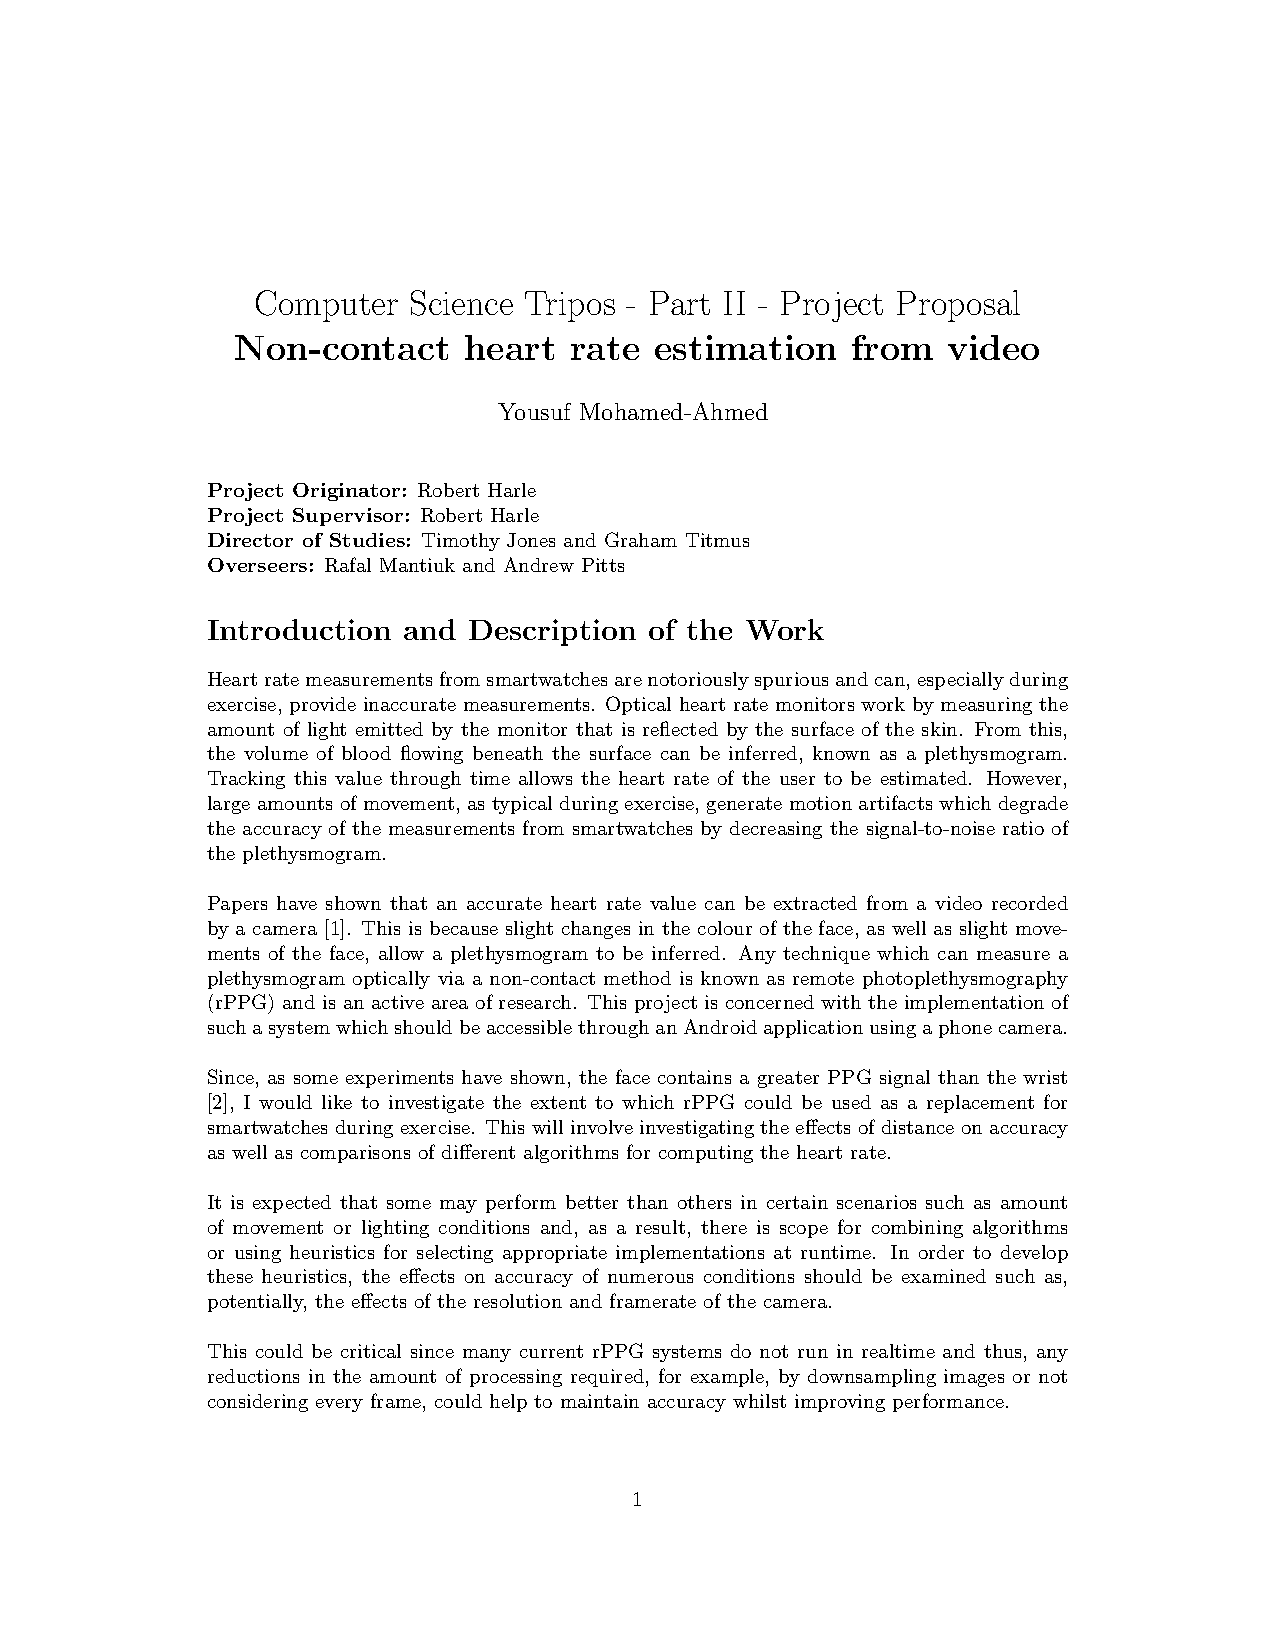
\includepdf[pages=-,pagecommand={},width=\paperwidth]{proposal/main.pdf}

\end{document}
